\documentclass[twoside]{book}

% Packages required by doxygen
\usepackage{fixltx2e}
\usepackage{calc}
\usepackage{doxygen}
\usepackage[export]{adjustbox} % also loads graphicx
\usepackage{graphicx}
\usepackage[utf8]{inputenc}
\usepackage{makeidx}
\usepackage{multicol}
\usepackage{multirow}
\PassOptionsToPackage{warn}{textcomp}
\usepackage{textcomp}
\usepackage[nointegrals]{wasysym}
\usepackage[table]{xcolor}

% Font selection
\usepackage[T1]{fontenc}
\usepackage[scaled=.90]{helvet}
\usepackage{courier}
\usepackage{amssymb}
\usepackage{sectsty}
\renewcommand{\familydefault}{\sfdefault}
\allsectionsfont{%
  \fontseries{bc}\selectfont%
  \color{darkgray}%
}
\renewcommand{\DoxyLabelFont}{%
  \fontseries{bc}\selectfont%
  \color{darkgray}%
}
\newcommand{\+}{\discretionary{\mbox{\scriptsize$\hookleftarrow$}}{}{}}

% Page & text layout
\usepackage{geometry}
\geometry{%
  a4paper,%
  top=2.5cm,%
  bottom=2.5cm,%
  left=2.5cm,%
  right=2.5cm%
}
\tolerance=750
\hfuzz=15pt
\hbadness=750
\setlength{\emergencystretch}{15pt}
\setlength{\parindent}{0cm}
\setlength{\parskip}{0.2cm}
\makeatletter
\renewcommand{\paragraph}{%
  \@startsection{paragraph}{4}{0ex}{-1.0ex}{1.0ex}{%
    \normalfont\normalsize\bfseries\SS@parafont%
  }%
}
\renewcommand{\subparagraph}{%
  \@startsection{subparagraph}{5}{0ex}{-1.0ex}{1.0ex}{%
    \normalfont\normalsize\bfseries\SS@subparafont%
  }%
}
\makeatother

% Headers & footers
\usepackage{fancyhdr}
\pagestyle{fancyplain}
\fancyhead[LE]{\fancyplain{}{\bfseries\thepage}}
\fancyhead[CE]{\fancyplain{}{}}
\fancyhead[RE]{\fancyplain{}{\bfseries\leftmark}}
\fancyhead[LO]{\fancyplain{}{\bfseries\rightmark}}
\fancyhead[CO]{\fancyplain{}{}}
\fancyhead[RO]{\fancyplain{}{\bfseries\thepage}}
\fancyfoot[LE]{\fancyplain{}{}}
\fancyfoot[CE]{\fancyplain{}{}}
\fancyfoot[RE]{\fancyplain{}{\bfseries\scriptsize Generated on Wed Aug 31 2016 14\+:29\+:33 for C\+L\+A\+S\+S-\/\+C\+T\+E\+M Documentation by Doxygen }}
\fancyfoot[LO]{\fancyplain{}{\bfseries\scriptsize Generated on Wed Aug 31 2016 14\+:29\+:33 for C\+L\+A\+S\+S-\/\+C\+T\+E\+M Documentation by Doxygen }}
\fancyfoot[CO]{\fancyplain{}{}}
\fancyfoot[RO]{\fancyplain{}{}}
\renewcommand{\footrulewidth}{0.4pt}
\renewcommand{\chaptermark}[1]{%
  \markboth{#1}{}%
}
\renewcommand{\sectionmark}[1]{%
  \markright{\thesection\ #1}%
}

% Indices & bibliography
\usepackage{natbib}
\usepackage[titles]{tocloft}
\setcounter{tocdepth}{3}
\setcounter{secnumdepth}{5}
\makeindex

% Hyperlinks (required, but should be loaded last)
\usepackage{ifpdf}
\ifpdf
  \usepackage[pdftex,pagebackref=true]{hyperref}
\else
  \usepackage[ps2pdf,pagebackref=true]{hyperref}
\fi
\hypersetup{%
  colorlinks=true,%
  linkcolor=blue,%
  citecolor=blue,%
  unicode%
}

% Custom commands
\newcommand{\clearemptydoublepage}{%
  \newpage{\pagestyle{empty}\cleardoublepage}%
}


%===== C O N T E N T S =====

\begin{document}

% Titlepage & ToC
\hypersetup{pageanchor=false,
             bookmarks=true,
             bookmarksnumbered=true,
             pdfencoding=unicode
            }
\pagenumbering{roman}
\begin{titlepage}
\vspace*{7cm}
\begin{center}%
{\Large C\+L\+A\+S\+S-\/\+C\+T\+E\+M Documentation }\\
\vspace*{1cm}
{\large Generated by Doxygen 1.8.9.1}\\
\vspace*{0.5cm}
{\small Wed Aug 31 2016 14:29:33}\\
\end{center}
\end{titlepage}
\clearemptydoublepage
\tableofcontents
\clearemptydoublepage
\pagenumbering{arabic}
\hypersetup{pageanchor=true}

%--- Begin generated contents ---
\chapter{C\+L\+A\+S\+S-\/\+C\+T\+E\+M Documentation}
\label{index}\hypertarget{index}{}\hypertarget{index_overviewCTEM}{}\section{Overview of the Canadian Terrestrial Ecosystem Model (\+C\+T\+E\+M)}\label{index_overviewCTEM}
Version 1 of the C\+T\+E\+M is the terrestrial carbon cycle component of the second generation Canadian Earth System Model (Can\+E\+S\+M2) \cite{Arora2011-79f} where it is coupled to version 2.\+7 of the Canadian Land Surface Scheme (C\+L\+A\+S\+S). C\+T\+E\+M v. 2.\+0 \cite{Melton2016-zx} is currently coupled to the C\+L\+A\+S\+S v. 3.\+6 \cite{Verseghy2012-c0e}. The coupled C\+L\+A\+S\+S--C\+T\+E\+M model is capable of being run online in the Can\+E\+S\+M model or offline, as is the case in this study, driven by observation-\/based meteorological forcings. C\+T\+E\+M models terrestrial ecosystem processes for nine P\+F\+Ts, two of which are crop P\+F\+Ts (see Table tab\+:compparams\}), by tracking the flow of carbon through three living vegetation components (leaves, stem and roots) and two dead carbon pools (litter and soil). The carbon budget equations for the model\textquotesingle{}s five pools are summarized in Sect. rate\+\_\+change\+\_\+eqns\} of the Appendix. The amount of carbon in these five carbon pools is simulated prognostically. C\+L\+A\+S\+S models the land surface energy and water balance and calculates liquid and frozen soil moisture, and soil temperature for three soil layers (with thicknesses 0.\+1, 0.\+25 and 3.\+75\textbackslash{}, $m$). In the C\+L\+A\+S\+S--C\+T\+E\+M framework, C\+L\+A\+S\+S uses structural vegetation attributes (including L\+A\+I, vegetation height, canopy mass and rooting depth) simulated by C\+T\+E\+M, and C\+T\+E\+M uses soil moisture, soil temperature and net radiation calculated by C\+L\+A\+S\+S. Combined, C\+L\+A\+S\+S and C\+T\+E\+M simulate the atmosphere--land fluxes of energy, water and $CO_2$.

Version 1.\+0 of C\+T\+E\+M is described in a collection of papers detailing parametrization of photosynthesis, autotrophic and heterotrophic respiration \cite{Arora2003-3b7}; phenology, carbon allocation, biomass turnover and conversion of biomass to structural attributes \cite{Arora2005-6b1}; dynamic root distribution \cite{Arora2003838}; and disturbance (fire) \cite{Arora20052ac}. These processes are modelled over prescribed fractional coverage of nine P\+F\+Ts \cite{Wang2006-he} and determine the structural vegetation dynamics including vegetation biomass, L\+A\+I, vegetation height, fraction of roots in each of the three soil layers, leaf onset and offset times and primary $CO_2$ fluxes of gross primary productivity (G\+P\+P) and N\+P\+P. A full description of C\+T\+E\+M and changes from v. 1.\+0 to v. 2.\+0 are included in the Appendix.

A parametrization for competition between P\+F\+Ts in an earlier version of C\+T\+E\+M is described by \cite{Arora2006-pp} \cite{Arora2006-ax} where it was evaluated at select locations. Here we present C\+T\+E\+M v. 2.\+0, which builds upon the model framework of C\+T\+E\+M v. 1.\+0 and can be run in two different modes, either (i) using specified fractional coverage of its nine P\+F\+Ts, or (ii) allowing the fractional coverage of its seven non-\/crop P\+F\+Ts to be dynamically determined based on competition between P\+F\+Ts. The parametrization for simulating competition between P\+F\+Ts is summarized in Sect. compmain\}. The fire parametrization has also been refined in the new model version as described in Appendix fire\}. The C\+L\+A\+S\+S--C\+T\+E\+M modelling framework has the capability of representing the sub-\/grid scale variability of P\+F\+Ts using either a composite or a mosaic configuration \cite{Li2012-f7f} \cite{Melton2014-xk}. In the composite (or single tile) configuration, the vegetation attributes for all P\+F\+Ts present in a grid cell are averaged and used in energy and water balance calculations that determine the physical land surface conditions including soil moisture, soil temperature and thickness and fractional coverage of snow (if present). In the mosaic (or multi-\/tile) configuration each P\+F\+T is allocated its own tile for which separate energy and water balance calculations are performed. As a result, the simulated carbon balance evolves somewhat differently in the two configurations despite being driven with identical climate forcing (see \cite{Melton2014-xk}). The results presented in this paper are obtained using the composite configuration.\hypertarget{index_overviewCLASS}{}\section{Overview of the Canadian Land Surface Scheme (\+C\+L\+A\+S\+S)}\label{index_overviewCLASS}
The Canadian Land Surface Scheme, C\+L\+A\+S\+S, was originally developed for use with the Canadian Global Climate Model or G\+C\+M (Verseghy, 1991; Verseghy et al., 1993). This documentation describes version 3.\+6 of C\+L\+A\+S\+S, which was released in December of 2011. The table at the end of this overview summarizes the development of C\+L\+A\+S\+S from the late 1980’s to the present.

The basic function of C\+L\+A\+S\+S is to integrate the energy and water balances of the land surface forward in time from an initial starting point, making use of atmospheric forcing data to drive the simulation. When C\+L\+A\+S\+S is run in coupled mode with a global or regional atmospheric model, the required forcing data are passed to it at each time step over each modeled grid cell from the atmospheric driver. C\+L\+A\+S\+S then performs its internal calculations, evaluating a suite of prognostic and diagnostic variables such as albedo and surface radiative and turbulent fluxes, which are in turn passed back to the driver. C\+L\+A\+S\+S can also be run in uncoupled or offline mode, using forcing data derived from field measurements, and the output values of its prognostic and diagnostic variables can then be validated against observations. Version 3.\+6 includes a single-\/column offline driver which can be used for this purpose.

C\+L\+A\+S\+S models separately the energy and water balances of the soil, snow, and vegetation canopy (see the diagram below). The basic prognostic variables consist of the temperatures and the liquid and frozen moisture contents of the soil layers; the mass, temperature, density, albedo and liquid water content of the snow pack; the temperature of the vegetation canopy and the mass of intercepted rain and snow present on it; the temperature and depth of ponded water on the soil surface; and an empirical vegetation growth index. These variables must be initialized, and a set of physical parameters describing the soil and vegetation existing on the modelled area must be assigned background values, at the beginning of the simulation.

At each time step, C\+L\+A\+S\+S calculates the bulk characteristics of the vegetation canopy on the basis of the vegetation types present over the modelled area. In a pre-\/processing step, each vegetation type is assigned representative values of parameters such as albedo, roughness length, annual maximum and minimum plant area index, rooting depth and so on (see the section on “\+Data Requirements”). These values are then aggregated over four main vegetation categories identified by C\+L\+A\+S\+S\+: needleleaf trees, broadleaf trees, crops, and grass (i.\+e. short vegetation). The physiological characteristics of the vegetation in each category are determined at the current time step using the aggregated background parameters and assumed annual or diurnal variation functions. These physiological characteristics are then aggregated to produce the bulk canopy characteristics for the current time step.


\begin{DoxyImage}
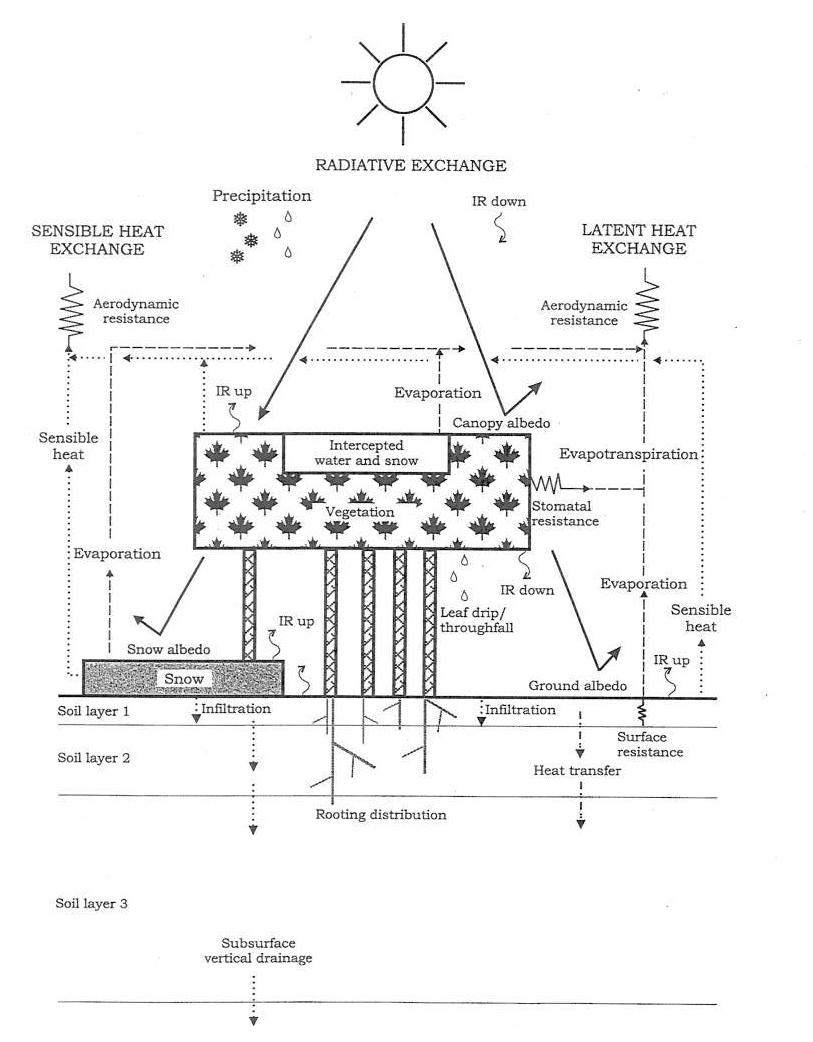
\includegraphics[width=\textwidth,height=\textheight/2,keepaspectratio=true]{schematicDiagramOfClass.png}
\caption{Schematic Diagram Of C\+L\+A\+S\+S}
\end{DoxyImage}
 In performing the surface flux calculations the modeled area is divided into up to four subareas\+: bare soil, vegetation over soil, snow over bare soil, and vegetation over snow. The fractional snow coverage is determined using the concept of a threshold snow depth. If the calculated snow depth is less than this value, the snow depth is set to the threshold value and the fractional snow cover is calculated on the basis of conservation of snow mass. The fluxes are calculated for each of the four subareas, and these and the prognostic variables are then areally averaged before being passed back to the atmospheric model.

Originally C\+L\+A\+S\+S performed only one set of these calculations for each grid cell of the model domain. In more recent versions, a “mosaic” option has been added to handle sub-\/grid scale heterogeneity more effectively. When this option is utilized, each grid cell is divided into a user-\/specified number of mosaic “tiles”, and the C\+L\+A\+S\+S calculations are performed in turn over each. The surface fluxes are averaged, but the prognostic variables are kept separate for each of the tiles of the mosaic between time steps.

The section on the C\+L\+A\+S\+S offline driver, R\+U\+N\+C\+L\+A\+S\+S, provides information on how a C\+L\+A\+S\+S run is typically performed, from assigning the background and initial values of variables, through calling the high-\/level C\+L\+A\+S\+S subroutines, to calculating values of diagnostic and output variables. A gather-\/scatter operation is included in the driver, mimicking the practice in atmospheric models of “gathering” land surface points on latitude circles onto long vectors prior to the calculations, for improved computational efficiency on vector supercomputers. For C\+L\+A\+S\+S, the mosaic tiles on each of the modelled grid cells are “gathered” onto long arrays prior to calling the C\+L\+A\+S\+S subroutines (thus collapsing the first two dimensions of the arrays into one), and subsequently “scattered” back onto the grid cells before performing the diagnostic averaging calculations.

The two sections following the one that describes the driver provide detailed descriptions first of the common block and other preliminary routines that are called before the run is launched, and then of the pre-\/ and post-\/processing routines that are called at the beginning and end of each time step. The next three sections detail the three main C\+L\+A\+S\+S subroutines together with the auxiliary subroutines that they call\+: C\+L\+A\+S\+S\+A, which handles the calculation of the albedos and other surface parameters; C\+L\+A\+S\+S\+T, which addresses the evaluation of the surface energy balance and related variables; and C\+L\+A\+S\+S\+W, which performs the surface water balance calculations and the re-\/aggregation of the prognostic variables. The sub-\/section on each subroutine contains a dictionary of the variables passed into and out of it, with units. The final section provides a list of references cited.\hypertarget{index_devHistory}{}\subsection{Developmental history of C\+L\+A\+S\+S}\label{index_devHistory}
\[ \begin{tabular}{ | l | l || l | } 1.0 & April 1989 & Basic thermal and hydrological model of snow and soil. \\ 2.0 & August 1991 & Addition of vegetation thermal and hydrological model. \\ 2.1 & May 1993 & Full vectorization of code to enable efficienr running on vector supercomputers. \\ 2.2 & April 1994 & Augmentation of diagnostic calculations; incorporation of in-line comments throughout; development \\ & & of a parallel stand-alone version of the model for use with field data. \\ 2.3 & December 1994 & Revisions to diagnostic calculations; new near-surface atmospheric stability functions. \\ 2.4 & August 1995 & Complete set of water budget diagnostic calculations; parametrizations of organic soils and \\ & &rock soils; allowance for inhomegeneity between soil layers; incorporation of variable \\ & & surface detention capacity. \\ 2.5 & January 1996 & Completion of energy budget diagnostic calculations. \\ 2.6 & August 1997 & Revisions to surface stability function calculations. \\ 2.7 & December 1997 & Incorporation of variable soil permeable depth; calculation of soil thermal and hydraulic \\ & & properties based on textural composition; modified surface temperature iteration scheme. \\ 3.0 & December 2002 & Improved treatment of soil evaporation; complete treatment of organic soils; new canopy \\ & & conductance formulation; preliminary routines for lateral movement of soil water; enhanced snow \\ & & density and snow interception; improved turbulent transfer from vegetation; mosaic formulation. \\ 3.1 & April 2005 & Faster surface temperature iteration scheme; refinements to leaf boundary resistance formulation; \\ & & improved treatment of snow sublimation and interception; transition to Fortran 90 and\\ & & single precision variables. \\ 3.2 & May 2006 & Option for multiple soil layers at depth; additional liquid water content of snow pack; revised radiation \\ & & transmission in vegetation. \\ 3.3 & December 2006 & Separate temperature profile curve fit for snow and soil; multiple-layer option for ice sheets;\\ & & water and energy balance checks for each time step; modifications to soil hydraulic \\ & & conductivity calculations. \\ 3.4 & April 2008 & Streamline and clean up code; updated soil thermal conductivity calculations; revisions to handling of\\ & & water stored on vegetation. \\ 3.5 & December 2010 & Updated field capacity calculation; revised treatment of water on canopy; \\ & & reworked calculation of baseflow. \\ 3.6 & December 2011 & Revised ponding depth over organic soils; revised snow albedo refreshment \\ & & threshold; new snow thermal conductivity algorithm; interface with Canadian Terrestrial \\ & & Ecosystem Model (CTEM). \\ \end{tabular} \]\hypertarget{index_dataRequirements}{}\section{Data Requirements}\label{index_dataRequirements}
This section describes the three types of data that are required to run C\+L\+A\+S\+S\+: atmospheric forcing data, surface vegetation and soil data, and initial values for the prognostic variables.\hypertarget{index_forcingData}{}\subsection{Forcing Data}\label{index_forcingData}
At each time step, for each grid cell or modelled area, the following atmospheric forcing data are required\+:


\begin{DoxyItemize}
\item F\+C\+L\+O\+R\+O\+W Fractional cloud cover \mbox{[} \mbox{]}
\item F\+D\+L\+R\+O\+W Downwelling longwave sky radiation $[ W m^{-2} ]$
\item F\+S\+I\+H\+R\+O\+W Near infrared shortwave radiation incident on a horizontal surface $[W m^{-2} ]$
\item F\+S\+V\+H\+R\+O\+W Visible shortwave radiation incident on a horizontal surface $[W m^{-2} ]$
\item P\+R\+E\+R\+O\+W Surface precipitation rate $[kg m^{-2} s^{-1} ]$
\item P\+R\+E\+S\+R\+O\+W Surface air pressure $[P_a ]$
\item Q\+A\+R\+O\+W Specific humidity at reference height $[kg kg^{-1} ]$
\item T\+A\+R\+O\+W Air temperature at reference height \mbox{[}K\mbox{]}
\item U\+L\+R\+O\+W Zonal component of wind velocity $[m s^{-1} ]$
\item V\+L\+R\+O\+W Meridional component of wind velocity $[m s^{-1} ]$
\item V\+M\+O\+D\+R\+O\+W Wind speed at reference height $[m s^-1 ]$
\item Z\+B\+L\+D\+R\+O\+W Atmospheric blending height for surface roughness length averaging \mbox{[}m\mbox{]}
\item Z\+R\+F\+H\+R\+O\+W Reference height associated with forcing air temperature and humidity \mbox{[}m\mbox{]}
\item Z\+R\+F\+M\+R\+O\+W Reference height associated with forcing wind speed \mbox{[}m\mbox{]}
\end{DoxyItemize}

When assembling the forcing data, the following guidelines should be noted\+:

1) C\+L\+A\+S\+S ordinarily requires that the forcing incoming shortwave radiation be partitioned into the visible and near-\/infrared components. If these are not available, however, they can each be roughly estimated as approximately half of the total incoming solar radiation.

2) The fractional cloud cover is used to calculate the direct and diffuse components of the incoming shortwave radiation. If it is not available it can be estimated on the basis of the solar zenith angle and the occurrence of precipitation (see the section on the R\+U\+N\+C\+L\+A\+S\+S driver).

3) For atmospheric models, the air temperature supplied to C\+L\+A\+S\+S should be the lowest level air temperature extrapolated using the dry adiabatic lapse rate to the bottom of the atmosphere, i.\+e. to where the wind speed is zero and the pressure is equal to the surface pressure P a . For field data, the actual measured air temperature at the reference height should be used, since in this case the adiabatic extrapolation is performed within C\+L\+A\+S\+S.

4) Atmospheric models provide the zonal and meridional components of the wind velocity, but C\+L\+A\+S\+S does not actually require information on wind direction. Thus, if only the scalar wind speed is available, either U\+L\+R\+O\+W or V\+L\+R\+O\+W can be set to it, and the other to zero. (Both of these terms, plus the scalar wind speed V\+M\+O\+D\+R\+O\+W, must be supplied to C\+L\+A\+S\+S.)

5) In atmospheric models the forcing wind speed, air temperature and specific humidity are obtained from the lowest modelled atmospheric layer, and thus the reference height will be the height above the “surface” (i.\+e. the location where the wind speed is zero and the pressure is equal to the surface pressure P a ) corresponding to that lowest layer. Some atmospheric models use a vertical co-\/ordinate system in which the momentum and thermodynamic levels are staggered, and if so, Z\+F\+R\+M\+R\+O\+W and Z\+R\+F\+H\+R\+O\+W will have different values. If that is the case, the switch I\+S\+L\+F\+D in the C\+L\+A\+S\+S driver should be set to 2, so that the subroutines F\+L\+X\+S\+U\+R\+F\+Z and D\+I\+A\+S\+U\+R\+F\+Z are called (see the R\+U\+N\+C\+L\+A\+S\+S documentation), since the other options do not support different reference heights. In the case of field data, the reference height is the height above the ground surface at which the variables are measured. If the measurement height for wind speed is different from that for the air temperature and specific humidity, again the I\+S\+L\+F\+D switch in the C\+L\+A\+S\+S driver should be set to 2. (Note that neither Z\+R\+F\+H\+R\+O\+W nor Z\+R\+F\+M\+R\+O\+W may be smaller than the vegetation canopy height, as this will cause the model run to crash.)

6) If the surface being modelled is a heterogeneous one, care must be taken to ensure that the reference heights are greater than the “blending height”, the distance above the surface at which the atmospheric variables are not dominated by any one surface type. In principle this height depends on the length scale of the roughness elements; it is usually of the order of 50-\/100 m. In C\+L\+A\+S\+S the blending height is used in averaging the roughness lengths over the modelled area, and is read in separately from Z\+R\+F\+M\+R\+O\+W and Z\+R\+F\+H\+R\+O\+W as Z\+B\+L\+D\+R\+O\+W.

7) C\+L\+A\+S\+S is able to run with total incoming precipitation, partitioning it into rainfall and snowfall on the basis of empirically derived equations. If the rainfall rate (R\+P\+R\+E\+R\+O\+W) and snowfall rate (S\+P\+R\+E\+R\+O\+W) are available, they should be used instead. The R\+E\+A\+D statement in the C\+L\+A\+S\+S driver should be modified accordingly, and the switch I\+P\+C\+P should be set to 4.

8) The length of the time step should be carefully considered in assembling the forcing data. C\+L\+A\+S\+S has been designed to run at a time step of 30 minutes or less, and the explicit prognostic time stepping scheme used for the soil, snow and vegetation variables is based on this assumption. Longer time steps may lead to the appearance of numerical instabilities in the modelled prognostic variables.\hypertarget{index_vegetationData}{}\subsection{Vegetation Data}\label{index_vegetationData}
For each of the four main vegetation categories (needleleaf trees, broadleaf trees, crops and grass), the following data are required for each mosaic tile over each grid cell or modelled area\+:


\begin{DoxyItemize}
\item A\+L\+I\+C\+R\+O\+T Average near-\/\+I\+R albedo of vegetation category when fully-\/leafed \mbox{[} \mbox{]}
\item A\+L\+V\+C\+R\+O\+T Average visible albedo of vegetation category when fully-\/leafed \mbox{[} \mbox{]}
\item C\+M\+A\+S\+R\+O\+T Annual maximum canopy mass for vegetation category $[kg m^{-2} ]$
\item F\+C\+A\+N\+R\+O\+T Annual maximum fractional coverage of modelled area \mbox{[} \mbox{]}
\item L\+N\+Z0\+R\+O\+T Natural logarithm of maximum vegetation roughness length \mbox{[} \mbox{]}
\item P\+A\+M\+N\+R\+O\+T Annual minimum plant area index of vegetation category \mbox{[} \mbox{]}
\item P\+A\+M\+X\+R\+O\+T Annual maximum plant area index of vegetation category \mbox{[} \mbox{]}
\item P\+S\+G\+A\+R\+O\+T Soil moisture suction coefficient (used in stomatal resistance calculation) \mbox{[} \mbox{]}
\item P\+S\+G\+B\+R\+O\+T Soil moisture suction coefficient (used in stomatal resistance calculation) \mbox{[} \mbox{]}
\item Q\+A50\+R\+O\+T Reference value of incoming shortwave radiation (used in stomatal resistance calculation) $[W m^{-2} ]$
\item R\+O\+O\+T\+R\+O\+T Annual maximum rooting depth of vegetation category \mbox{[}m\mbox{]}
\item R\+S\+M\+N\+R\+O\+T Minimum stomatal resistance of vegetation category $[s m^{-1} ]$
\item V\+P\+D\+A\+R\+O\+T Vapour pressure deficit coefficient (used in stomatal resistance calculation) \mbox{[} \mbox{]}
\item V\+P\+D\+B\+R\+O\+T Vapour pressure deficit coefficient (used in stomatal resistance calculation) \mbox{[} \mbox{]}
\end{DoxyItemize}

C\+L\+A\+S\+S models the physiological characteristics of trees as remaining constant throughout the year except for the leaf area index and plant area index, which vary seasonally between the limits defined by P\+A\+M\+X\+R\+O\+T and P\+A\+M\+N\+R\+O\+T. The areal coverage of crops varies from zero in the winter to F\+C\+A\+N\+R\+O\+T at the height of the growing season, and their physiological characteristics undergo a corresponding cycle. Grasses remain constant year-\/round. (For full details of these calculations, see the documentation for subroutine A\+P\+R\+E\+P). Urban areas are also treated as “vegetation” in the C\+L\+A\+S\+S code, and have associated values for F\+C\+A\+N\+R\+O\+T, A\+L\+V\+C\+R\+O\+T, A\+L\+I\+C\+R\+O\+T and L\+N\+Z0\+R\+O\+T. Thus these arrays have a third dimension of 5 rather than 4.

Ideally the above vegetation parameters should be measured at the modelled location. Of course this is not always possible, especially when running over a large modelling domain. As a guide, the table in Appendix A provides representative values for the 20 vegetation types recognized by the Canadian G\+C\+M. If more than one type of vegetation in a given category is present on the modelled area, the parameters for the category should be areally averaged over the vegetation types present. For the stomatal resistance parameters, typical values of these for the four principal vegetation types are given below\+:

\[ \begin{tabular}{ | l | c | c | c | c | c | c | } & RSMN & QA50 & VPDA & VPDB & PSGA & PSGB \\ Needleleaf trees & 200.0 & 30.0 & 0.65 & 1.05 & 100.0 & 5.0 \\ Broadleaf trees & 125.0 & 40.0 & 0.50 & 0.60 & 100.0 & 5.0 \\ Crops & 85.0 & 30.0 & 0.50 & 1.00 & 100.0 & 5.0 \\ Grass & 100.0 & 30.0 & 0.50 & 1.00 & 100.0 & 5.0 \\ \end{tabular} \]\hypertarget{index_soilData}{}\subsection{Soil Data}\label{index_soilData}
The following information is required for each modelled soil layer\+:


\begin{DoxyItemize}
\item D\+E\+L\+Z Layer thickness \mbox{[}m\mbox{]}
\item Z\+B\+O\+T Depth of bottom \mbox{[}m\mbox{]}
\end{DoxyItemize}

The standard operational configuration for C\+L\+A\+S\+S consists of three soil layers, of thicknesses 0.\+10 m, 0.\+25 m and 3.\+75 m, and thus of bottom depths 0.\+10, 0.\+35 and 4.\+10 m respectively. C\+L\+A\+S\+S versions 3.\+2 and higher support other options\+: the third soil layer may be replaced with a larger number of thinner layers, and/or the bottom of the soil profile may be extended below 4.\+10 m. However, because the temperature stepping scheme used in C\+L\+A\+S\+S is of an explicit formulation, care must be taken not to make the layers too thin, since this may lead to numerical instability problems.

For each of the modelled soil layers on each of the mosaic tiles, the following texture data are required\+:


\begin{DoxyItemize}
\item C\+L\+A\+Y\+R\+O\+T Percentage clay content
\item O\+R\+G\+M\+R\+O\+T Percentage organic matter content
\item S\+A\+N\+D\+R\+O\+T Percentage sand content
\end{DoxyItemize}


\begin{DoxyImage}
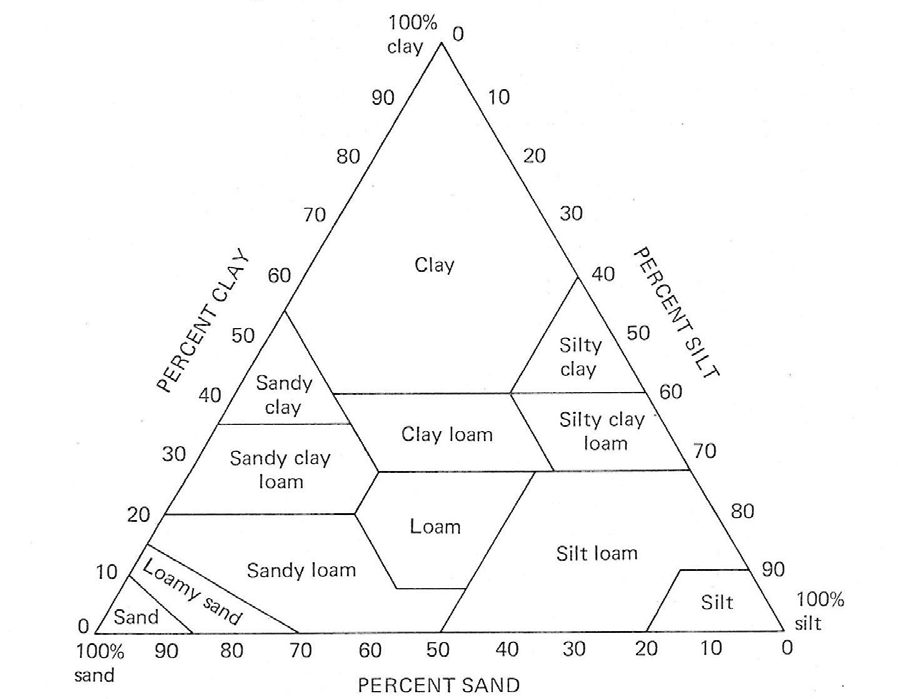
\includegraphics[width=\textwidth,height=\textheight/2,keepaspectratio=true]{percentSand.png}
\caption{Percent Sand}
\end{DoxyImage}
 1) For mineral soils, the percentages of sand, clay and organic matter content need not add up to 100\%, since the residual is assigned to silt content. If the exact sand, clay and organic matter contents are not known, estimates can be made for the general soil type on the basis of the standard U\+S\+D\+A texture triangle shown above. Organic matter contents in mineral soils are typically not more than a few percent.

2) If the soil layer is a fully organic one, S\+A\+N\+D\+R\+O\+T, C\+L\+A\+Y\+R\+O\+T and O\+R\+G\+M\+R\+O\+T are used differently. The sand content is assigned a flag value of -\/2, and the organic matter content may be assigned a flag value of 1, 2 or 3 depending on whether the peat texture is fibric, hemic or sapric (see Letts et al., 2000). The current default is for the first layer to be assumed as fibric, the second as hemic and any lower layers as sapric. C\+L\+A\+Y\+R\+O\+T is not used and is set to zero.

3) If the layer consists of rock, S\+A\+N\+D\+R\+O\+T is assigned a flag value of -\/3. If it is part of a continental ice sheet, it is assigned a flag value of -\/4. In both cases, C\+L\+A\+Y\+R\+O\+T and O\+R\+G\+M\+R\+O\+T are not used and are set to zero.

S\+A\+N\+D\+R\+O\+T, C\+L\+A\+Y\+R\+O\+T and O\+R\+G\+M\+R\+O\+T are utilized in the calculation of the soil layer thermal and hydraulic properties in subroutine C\+L\+A\+S\+S\+B. If the measured values of these properties are available, they should be used instead.

For each of the mosaic tiles over the modelled area, the following surface parameters must be specified\+:


\begin{DoxyItemize}
\item D\+R\+N\+R\+O\+T Soil drainage index
\item F\+A\+R\+E\+R\+O\+T Fractional coverage of mosaic tile on the modelled area
\item M\+I\+D\+R\+O\+T Mosaic tile type identifier (1 for land surface, 0 for inland lake)
\item S\+D\+E\+P\+R\+O\+T Soil permeable depth \mbox{[}m\mbox{]}
\end{DoxyItemize}

1) The soil permeable depth, i.\+e. the depth to bedrock, may be less than the modelled thermal depth of the soil profile. This permeable depth is indicated by the variable S\+D\+E\+P\+R\+O\+T. If the depth to bedrock occurs within a soil layer rather than at the interface between two layers, C\+L\+A\+S\+S assigns the specified mineral or organic soil characteristics to the part of the layer above bedrock, and values corresponding to rock to the portion below.

2) The drainage index, D\+R\+N\+R\+O\+T, is set to 1 except in cases of deep soils where it is desired to suppress drainage from the bottom of the soil profile (e.\+g. in bogs, or in deep soils with a high water table). In this case it is set to 0.

When the standard three-\/layer soil configuration is used, C\+L\+A\+S\+S provides a means of accounting for the possibility of the depth to bedrock falling within the thick third layer, and therefore of phase changes of water taking place in only the upper part of the layer, by introducing the variable T\+B\+A\+S\+R\+O\+T, which refers to the temperature of the lower part of the layer containing the bedrock. At the beginning of the time step the temperature of the upper part of the layer is disaggregated from the overall average layer temperature using the saved value of T\+B\+A\+S\+R\+O\+T. The heat flow between the upper part of the soil layer and the lower part is diagnosed from the heat flux at the top of the layer. The upper layer temperature and T\+B\+A\+S\+R\+O\+T are stepped ahead separately, and the net heat flux in the upper part of the layer is used in the phase change of water if appropriate. The upper layer temperature and T\+B\+A\+S\+R\+O\+T are re-\/aggregated at the end of the time step to yield once again the overall average layer temperature.

Two variables, assumed to be constant over the grid cell, are provided if required for atmospheric model runs\+:


\begin{DoxyItemize}
\item G\+G\+E\+O\+R\+O\+W Geothermal heat flux $[W m^{-2} ]$
\item Z0\+O\+R\+R\+O\+W Orographic roughness length \mbox{[}m\mbox{]}
\end{DoxyItemize}

Unless the soil depth is very large and/or the run is very long, the geothermal heat flux can be set to zero. Z0\+O\+R\+R\+O\+W is the surface roughness length representing the contribution of orography or other terrain effects to the overall roughness, which becomes important when the modelled grid cell is very large (e.\+g. in a G\+C\+M). For field studies it can be set to zero.

Finally, four parameters are required for modelling lateral movement of soil water\+: G\+R\+K\+F\+R\+O\+T, W\+F\+C\+I\+R\+O\+T, W\+F\+S\+F\+R\+O\+T and X\+S\+L\+P\+R\+O\+T. However, the routines for interflow and streamflow modelling are still under development, so unless the user is involved in this development, these parameters can be set to arbitrary values, since they will not be used.\hypertarget{index_initProgVar}{}\subsection{Initialization of Prognostic Variables}\label{index_initProgVar}
C\+L\+A\+S\+S requires initial values of the land surface prognostic variables, either from the most recent atmospheric model integration or from field measurements. These are listed below, with guidelines for specifying values for each.


\begin{DoxyItemize}
\item A\+L\+B\+S\+R\+O\+T Snow albedo \mbox{[} \mbox{]}
\item C\+M\+A\+I\+R\+O\+T Aggregated mass of vegetation canopy $[kg m^{-2} ]$
\item G\+R\+O\+R\+O\+T Vegetation growth index \mbox{[} \mbox{]}
\item Q\+A\+C\+R\+O\+T Specific humidity of air within vegetation canopy space $[kg kg^{-1} ]$
\item R\+C\+A\+N\+R\+O\+T Intercepted liquid water stored on canopy $[kg m^{-2} ]$
\item R\+H\+O\+S\+R\+O\+T Density of snow $[kg m^{-3} ]$
\item S\+C\+A\+N\+R\+O\+T Intercepted frozen water stored on canopy $[kg m^{-2} ]$
\item S\+N\+O\+R\+O\+T Mass of snow pack $[kg m^{-2} ]$
\item T\+A\+C\+R\+O\+T Temperature of air within vegetation canopy \mbox{[}K\mbox{]}
\item T\+B\+A\+R\+R\+O\+T Temperature of soil layers \mbox{[}K\mbox{]}
\item T\+B\+A\+S\+R\+O\+T Temperature of bedrock in third soil layer \mbox{[}K\mbox{]}
\item T\+C\+A\+N\+R\+O\+T Vegetation canopy temperature \mbox{[}K\mbox{]}
\item T\+H\+I\+C\+R\+O\+T Volumetric frozen water content of soil layers $[m^3 m^{-3} ]$
\item T\+H\+L\+Q\+R\+O\+T Volumetric liquid water content of soil layers $[m^3 m^{-3} ]$
\item T\+P\+N\+D\+R\+O\+T Temperature of ponded water \mbox{[}K\mbox{]}
\item T\+S\+F\+S\+R\+O\+T Ground surface temperature over subarea \mbox{[}K\mbox{]}
\item T\+S\+N\+O\+R\+O\+T Snowpack temperature \mbox{[}K\mbox{]}
\item W\+S\+N\+O\+R\+O\+T Liquid water content of snow pack $[kg m^{-2} ]$
\item Z\+P\+N\+D\+R\+O\+T Depth of ponded water on surface \mbox{[}m\mbox{]}
\end{DoxyItemize}

1) T\+B\+A\+R\+R\+O\+T, T\+H\+L\+Q\+R\+O\+T and T\+H\+I\+C\+R\+O\+T are required for each of the modelled soil layers. Thin soil layers near the surface equilibrate quickly, but thicker, deeper layers respond more slowly, and long-\/term biases can be introduced into the simulation if their temperatures and moisture contents are not initialized to reasonable values. For the moisture contents, it may be better to err on the low side, since soil moisture recharge typically takes place on shorter time scales than soil moisture loss. Field capacity is commonly used as an initial value. If the soil layer temperature is above freezing, the liquid moisture content would be set to the field capacity and the frozen moisture content to zero; if the layer temperature is below zero, the liquid moisture content would be set to the minimum value and the frozen moisture content to the field capacity minus the minimum value. Very deep soil temperatures do not have a large effect on surface fluxes, but errors in their initial values can adversely effect hydrological simulations. If the standard three-\/layer soil configuration is being used, T\+B\+A\+S\+R\+O\+T should be set to the third soil layer temperature; otherwise it can be arbitrarily set to zero. For rock or ice layers, T\+H\+L\+Q\+R\+O\+T and T\+H\+I\+C\+R\+O\+T should both be set to zero.

2) It is best to begin a simulation in snow-\/free conditions, so that the snow simulation can start from the simplest possible state where S\+N\+O\+R\+O\+T, T\+S\+N\+O\+R\+O\+T, A\+L\+B\+S\+R\+O\+T, R\+H\+O\+S\+R\+O\+T and W\+S\+N\+O\+R\+O\+T are all initialized to zero. If erroneous values of the snow variables are specified as initial conditions, this can lead to a persistent bias in the land surface simulation.

3) The vegetation canopy has a relatively small heat capacity and water storage capacity compared with the soil, so its temperature and intercepted water stores equilibrate quite quickly. T\+C\+A\+N\+R\+O\+T and T\+A\+C\+R\+O\+T can be initialized to the air temperature and Q\+A\+C\+R\+O\+T to the air specific humidity. R\+C\+A\+N\+R\+O\+T and S\+C\+A\+N\+R\+O\+T can be initialized to zero. C\+M\+A\+I\+R\+O\+T, which is used only in the diagnostic energy balance check during the time step, can also be set to zero.

4) G\+R\+O\+R\+O\+T should be initialized to 1 during the growing season and to 0 otherwise.

5) Surface ponded water is a small term and is ephemeral in nature, so Z\+P\+N\+D\+R\+O\+T and T\+P\+N\+D\+R\+O\+T can both be initialized to zero. T\+S\+F\+S\+R\+O\+T is included simply to provide a first guess for the surface temperature iteration in the next time step, so it can be initialized to an arbitrary value. For the snow-\/covered subareas of the surface it can be set to the freezing point of water; for the snow-\/free subareas it can be set to the temperature of the first soil layer.\hypertarget{index_runStandAloneMode}{}\section{Running C\+L\+A\+S\+S-\/\+C\+T\+E\+M}\label{index_runStandAloneMode}
Some points\+:
\begin{DoxyEnumerate}
\item runclass36ctem.\+f is the primary driver via which most input data is read (C\+T\+E\+M\textquotesingle{}s initialization files are read in \hyperlink{io__driver_8f90}{io\+\_\+driver.\+f90}) and subroutines are called.
\item The model initialization files include one for C\+L\+A\+S\+S (S\+I\+T\+E\+N\+A\+M\+E.\+I\+N\+I) and one for C\+T\+E\+M (S\+I\+T\+E\+N\+A\+M\+E.\+C\+T\+M). Examples provided in the Benchmarks folder.
\item The file containing meteorological data (S\+I\+T\+E\+N\+A\+M\+E.\+M\+E\+T). Also provided in the Benchmarks folder.
\item A Makefile is included which compiles all .f and .f90 files and generates an executable called C\+L\+A\+S\+S36\+C\+T\+E\+M. The standard Makefile, currently set up for pgf90 (but can also be setup for xlf and gfortran) may not be suitable for your Unix station and might require modification. You may need your system administrator’s help to do this. Note that when the code is compiled it generates .mod files that corresponds to the Fortran modules.
\end{DoxyEnumerate}

Other than the .I\+N\+I, .C\+T\+M and .M\+E\+T files which are mandatory, some other C\+T\+E\+M related files are also required depending on which C\+T\+E\+M functionality is switched on. These required files are discussed further down in this user guide.\hypertarget{index_compvsmosaic}{}\subsection{One thing to note about composite versus mosaic running of the model}\label{index_compvsmosaic}
In the composite mode, the structural vegetation attributes (including leaf area index, vegetation height, rooting depth) of P\+F\+Ts that exist in a grid cell are averaged in proportion to their fractional coverages and then used in the grid-\/averaged energy and water balance calculations. As a result the entire grid cell is characterized by land surface physical environment (including soil temperature, soil moisture, fractional snow cover, and net radiation) that is common to all P\+F\+Ts. In contrast, in the mosaic mode a grid box is split into multiple tiles representing individual P\+F\+Ts for each of which energy, water and carbon balance calculations are performed separately. The mosaic mode is, however, able to represent all forms of sub-\/grid scale variabilities. In principle, the mosaic mode may be used to represent tiles that are characterized by different soil types. For the purposes of coupling to C\+T\+E\+M, however, each tile represents each P\+F\+T.

In the composite mode then there is only one tile which covers the whole grid cell and the fractional coverage of C\+L\+A\+S\+S’s 4 P\+F\+Ts and C\+T\+E\+M’s 9 P\+F\+Ts are specified or dynamically modelled by C\+T\+E\+M. In the mosaic mode, the grid cell is divided into multiple tiles and each tile is assumed to be covered by only one P\+F\+T (for simplicity) although the entire grid cell is still assumed to be characterized by the same soil type. \cite{Melton2016-zx} describe the composite and mosaic approaches for the C\+L\+A\+S\+S-\/\+C\+T\+E\+M modelling framework.

Although pretty clever, running the mosaic version and interpreting the model results can be a logical nightmare, especially with competition on where the fractions of different tiles/mosaic change with time. So if you are new at this, please consider running the model in the composite mode.\hypertarget{index_inputs}{}\subsection{The Input Files}\label{index_inputs}
\hypertarget{index_MET}{}\subsubsection{The M\+E\+T file (\+Meteorological forcings)}\label{index_MET}
The .M\+E\+T files contain (usually) half-\/hourly values of all seven variables that are needed to drive the C\+L\+A\+S\+S land surface scheme. Please see the Benchmarks folder for an example .M\+E\+T file. The format of the .M\+E\+T file cannot be changed since C\+L\+A\+S\+S reads in these data using a fixed F\+O\+R\+T\+R\+A\+N format (1\+X,I2,I3,I5,I6,2\+F9.\+2,E14.\+4,F9.\+2,E12.\+3,F8.\+2,F12.\+2,3\+F9.\+2,F9.\+4).\hypertarget{index_INI}{}\subsubsection{The I\+N\+I file (\+C\+L\+A\+S\+S\textquotesingle{}s initialization file)}\label{index_INI}
The .I\+N\+I file is the initialization file for C\+L\+A\+S\+S, and includes initialization data for soil moisture, temperature, and other related fields. Like the .M\+E\+T file, the .I\+N\+I file also uses fixed F\+O\+R\+T\+R\+A\+N formats to read data, so caution must be taken when changing the .I\+N\+I file fields. In addition, note that when the code is run with dynamic vegetation (when C\+T\+E\+M is switched on) several of the vegetation-\/ related fields specified in the .I\+N\+I file are replaced by those estimated by C\+T\+E\+M. These fields include\+:


\begin{DoxyItemize}
\item Leaf area index (L\+A\+I)
\item Log of roughness length
\item Visible and near-\/infrared albedos
\item Canopy mass
\item Rooting depth
\end{DoxyItemize}

In addition, C\+T\+E\+M calculates stomatal resistance values so parameters related to C\+L\+A\+S\+S’ stomatal resistance formulation and the associated parameters in the .I\+N\+I file (R\+S\+M\+N, Q\+A50, V\+P\+D\+A, V\+P\+D\+B, P\+S\+G\+A and P\+S\+G\+B) do not matter.

If C\+L\+A\+S\+S is being run on its own, without C\+T\+E\+M, proper specification of vegetation related attributes and parameters is crucial.

Version 2.\+0 of C\+T\+E\+M adds the capability to divide each cell into several mosaics or ‘tiles’ as mentioned above. When running for multiple tiles, Both the C\+L\+A\+S\+S and C\+T\+E\+M calculations are performed over each tile. The prognostic variables are saved for each tile in addition to grid averaged values.

A sample .I\+N\+I file is found in the Benchmarks folder. The I\+N\+I file has very speficic formatting. You can see it in runclass36ctem.\+f where the I\+N\+I file is read and written (search for file units 10 and 100, respectively). Below is an explanation of the variables found in the I\+N\+I file\+:


\begin{DoxyItemize}
\item Z\+R\+F\+M and Z\+R\+F\+H (m)\+: The reference height at which the climate variables (wind speed, temperature and specific humidity) are provided. If the model is driven by the atmospheric model forcing data, these heights would vary by time step. If the model is driven by field data (such as the sample file here), these heights refer to the measurement height of these variables.
\item Z\+B\+L\+D (m)\+: Atmospheric blending height. Here it is assigned a value of 50 m.
\item G\+C\+: G\+C\+M surface description variable. For land surface (including inland water) it has a value of -\/1.
\item Plant growth index\+: C\+L\+A\+S\+S uses specified maximum and minimum leaf area indices (L\+A\+Is) for each of its four plant functional types (P\+F\+Ts). The L\+A\+I goes from this minimum to the maximum specified L\+A\+I at a specified rate and dependent on the soil temperature. Plant growth index determines what the L\+A\+I would be at initialization. This is little tricky if you aren’t familiar with C\+L\+A\+S\+S, so it’s best left at zero. In addition, when coupled to C\+T\+E\+M this doesn’t matter because then C\+L\+A\+S\+S uses L\+A\+I simulated by C\+T\+E\+M. When C\+T\+E\+M is switched on then all vegetation-\/related fields are estimated by C\+T\+E\+M. Competition between P\+F\+Ts is now simulated and so if a user switches on this option then the fractional coverage of P\+F\+Ts that grow in a grid cell is also simulated dynamically by C\+T\+E\+M. However, please read the discussion related to each of C\+T\+E\+M’s capabilities associated with each switch further down this user guide.
\item N\+L\+T\+E\+S\+T and N\+M\+T\+E\+S\+T\+: Number of grid cells and the number of mosaic tiles. N\+L\+T\+E\+S\+T can not be greater than N\+L\+A\+T. Also, N\+M\+T\+E\+S\+T must not be greater than N\+M\+O\+S. Typically this standalone code is run for 1 grid cell (N\+L\+T\+E\+S\+T=1) with 1 or more mosaic tiles (N\+M\+T\+E\+S\+T=1 or more).
\item R\+S\+M\+N (s m-\/1), Q\+A50 (W/m2), V\+P\+D\+A, V\+P\+D\+B, P\+S\+G\+A and P\+S\+G\+B\+: Used in stomatal resistance calculation in C\+L\+A\+S\+S subroutine C\+A\+N\+A\+L\+B. Note that these values do not matter when C\+T\+E\+M is switched on. Typical values for the four C\+L\+A\+S\+S vegetation categories are listed above in section {\bfseries Vegetation Data}.
\item D\+R\+N\+: Set it to 1 to allow drainage. Set it to 0 if drainage is suppressed at the bottom of the soil layer. Coupling of C\+L\+A\+S\+S 3.\+6 to C\+T\+E\+M required a lot of tuning because it seems C\+L\+A\+S\+S 3.\+6 is drier than C\+L\+A\+S\+S 2.\+7. As a result a value of 0.\+1 has been lately used the C\+C\+Cma Earth system model.
\item S\+D\+E\+P (m)\+: Depth to bedrock in the soil profile
\item X\+S\+L\+P, G\+R\+K\+F, W\+F\+S\+F, W\+F\+C\+I\+: Parameters used when running M\+E\+S\+H code, not used in Version 3.\+6 of C\+L\+A\+S\+S.
\item T\+B\+A\+R, T\+H\+L\+Q and T\+H\+I\+C\+: Thin soil layers near the surface equilibrate quickly, but thicker, deeper layers respond more slowly. Long-\/term biases can be introduced into the simulation if the soil layers temperatures and moisture contents are not initialized accurately. For the moisture contents, it is better to err on the low side, since soil moisture recharge typically takes place on shorter scales than soil moisture loss. Very deep soil temperatures do not have a large effect on surface fluxes, but errors in their initial values can affect hydrological simulations. For rock or ice layers, T\+H\+L\+Q and T\+H\+I\+C should both be set to zero.
\item R\+C\+A\+N (kg/m2)\+: Intercepted liquid water stored on canopy. R\+C\+A\+N can be initialized to zero.
\item S\+C\+A\+N (kg/m2)\+: Intercepted frozen water stored on canopy The vegetation canopy has a relatively small heat capacity and water storage capacity relative to the soil, so its temperature and intercepted water stores equilibrate quickly. T\+C\+A\+N can be initialized to the air temperature. S\+C\+A\+N can be initialized to zero.
\item S\+N\+O (kg/m2)\+: Mass of snow pack.
\item A\+L\+B\+S\+: Snow albedo.
\item R\+H\+O\+S (kg/m3)\+: Snow density
\end{DoxyItemize}

The above three variables and T\+S\+N\+O can be all initialized to 0 in snow-\/free conditions.


\begin{DoxyItemize}
\item T\+P\+N\+D and Z\+P\+N\+D\+: Surface ponded water is a small term and is ephemeral in nature, so Z\+P\+N\+D\+R\+O\+W and T\+P\+N\+D\+R\+O\+W can both be initialized to zero.
\item G\+R\+O\+: Vegetation growth index, should be initialized to 1 during the growing season and to 0 otherwise. If C\+T\+E\+M is switched on, these values do not matter.
\item D\+E\+L\+Z and Z\+B\+O\+T\+: The standard operational configuration for C\+L\+A\+S\+S consists of three soil layers, of thicknesses 0.\+10 m, 0.\+25 m and 3.\+75 m, and thus of bottom depths 0.\+10, 0.\+35 and 4.\+10 m respectively. Version 3.\+6 supports other options\+: the third soil layer may be replaced with a larger number of thinner layers, and/or the bottom of the soil profile may be extended below 4.\+10 m. However, care must be taken not to make the soil layers too thin since this may lead to numerical instability.
\end{DoxyItemize}\hypertarget{index_classvals}{}\subsubsection{Typical values of vegetation-\/related fields for C\+L\+A\+S\+S-\/only simulations}\label{index_classvals}
If you run C\+L\+A\+S\+S without C\+T\+E\+M you will need to specify all vegetation-\/related parameters. The table below shows typical values you may want to use for different vegetation types.

\[ \begin{tabular}{ | l | c | c | c | c | c | c | c | c | } Biome & CLASS PFT & Visible albedo & Near-infrared Albedo & Roughness length (m) \\ Needleleaf evergreen forest & 1 & 0.03 & 0.19 & 1.5 \\ Needleleaf deciduous forest & 1 & 0.03 & 0.19 & 1.0 \\ Broadleaf evergreen forest & 2 & 0.03 & 0.23 & 3.5 \\ Broadleaf cold deciduous forest & 2 & 0.05 & 0.29 & 2.0 \\ Broadleaf tropical evergreen forest & 2 & 0.03 & 0.23 & 3.0 \\ Broadleaf tropical drought deciduous forest & 2 & 0.05 & 0.29 & 0.8 \\ Broadleaf evergreen shrub & 4 & 0.03 & 0.19 & 0.05 \\ Broadleaf deciduous shrub & 2 & 0.05 & 0.29 & 0.15 \\ Broadleaf thorn shrub & 2 & 0.06 & 0.32 & 0.15 \\ Short grass and forbs & 4 & 0.06 & 0.34 & 0.02 \\ Long grass & 4 & 0.05 & 0.31 & 0.08 \\ Arable & 3 & 0.06 & 0.34 & 0.08 \\ Rice & 3 & 0.06 & 0.36 & 0.08 \\ Sugarcane & 3 & 0.05 & 0.31 & 0.35 \\ Maize & 3 & 0.05 & 0.33 & 0.25 \\ Cotton & 3 & 0.07 & 0.43 & 0.10 \\ Irrigated crop & 3 & 0.07 & 0.36 & 0.08 \\ Tundra & 4 & 0.05 & 0.29 & 0.01 \\ Swamp & 4 & 0.03 & 0.25 & 0.05 \\ Urban & 5 & 0.09 & 0.15 & 1.35 \\ \end{tabular} \]

\[ \begin{tabular}{ | l | c | c | c | c | c | c | c | c | } Biome & CLASS PFT & Max. LAI (m2/m2) & Min. LAI (m2/m2) & Aboveground biomass (kg/m2) & Rooting depth (m) \\ Needleleaf evergreen forest & 1 & 2.0 & 1.6 & 25.0 & 1.0 \\ Needleleaf deciduous forest & 1 & 2.0 & 0.5 & 15.0 & 1.0 \\ Broadleaf evergreen forest & 2 & 8.0 & 8.0 & 50.0 & 5.0 \\ Broadleaf cold deciduous forest & 6.0 & 0.5 & 20.0 & 2.0 \\ Broadleaf tropical evergreen forest & 8.0 & 8.0 & 40.0 & 5.0 \\ Broadleaf tropical drought deciduous forest & 4.0 & 4.0 & 15.0 & 5.0 \\ Broadleaf evergreen shrub & 2.0 & 2.0 & 2.0 & 0.2 \\ Broadleaf deciduous shrub & 4.0 & 0.5 & 8.0 & 1.0 \\ Broadleaf thorn shrub & 3.0 & 3.0 & 8.0 & 5.0 \\ Short grass and forbs & 3.0 & 3.0 & 1.5 & 1.2 \\ Long grass & 4.0 & 4.0 & 3.0 & 1.2 \\ Arable & 4.0 & 0.0 & 2.0 & 1.2 \\ Rice & 6.5 & 0.0 & 2.0 & 1.2 \\ Sugarcane & 5.0 & 0.0 & 5.0 & 1.0 \\ Maize & 4.0 & 0.0 & 5.0 & 1.5 \\ Cotton & 5.0 & 0.0 & 2.0 & 2.0 \\ Irrigated crop & 4.0 & 0.0 & 2.0 & 5.0 \\ Tundra & 1.5 & 1.5 & 0.2 & 0.1 \\ Swamp & 1.5 & 1.5 & 1.0 & 5.0 \\ Urban & - & - & - & - \\ \end{tabular} \] \hypertarget{index_classtoctem}{}\subsubsection{C\+L\+A\+S\+S and C\+T\+E\+M P\+F\+Ts}\label{index_classtoctem}
While C\+L\+A\+S\+S models all physical processes related to energy and water balance for four P\+F\+Ts, C\+T\+E\+M models its terrestrial ecosystem processes for nine P\+F\+Ts. The nine P\+F\+Ts of C\+T\+E\+M, however, line up with C\+L\+A\+S\+S’ four P\+F\+Ts perfectly as shown in Table 4. Needleleaf trees are divided into their evergreen and deciduous versions, broadleaf trees are divided into evergreen and cold and drought/dry deciduous versions, and crops and grasses are divided into their C3 and C4 versions based on their photosynthetic pathway.

\[ \begin{tabular}{ | l | c | c | } & CTEM PFTs & CLASS PFTs \\ 1. & Needleleaf Evergreen & Needleleaf \\ 2. & Needleleaf Deciduous & \\ 3. & Broadleaf Evergreen & Broadleaf \\ 4. & Broadleaf Cold Deciduous & \\ 5. & Broadleaf Drought/Dry Deciduous & \\ 6. & C3 Crop & Crops \\ 7. & C4 Crop & \\ 8. & C3 Grass & Grasses \\ 9. & C4 Grass & \\ \end{tabular} \] 
\chapter{Module Index}
\section{Modules}
Here is a list of all modules\+:\begin{DoxyCompactList}
\item \contentsline{section}{Competition\+\_\+scheme\+\_\+bioclim}{\pageref{group__competition__scheme__bioclim}}{}
\item \contentsline{section}{Competition\+\_\+scheme\+\_\+existence}{\pageref{group__competition__scheme__existence}}{}
\item \contentsline{section}{Competition\+\_\+scheme\+\_\+competition}{\pageref{group__competition__scheme__competition}}{}
\item \contentsline{section}{Ctem\+\_\+params\+\_\+initpftpars}{\pageref{group__ctem__params__initpftpars}}{}
\item \contentsline{section}{Disturbance\+\_\+scheme\+\_\+disturb}{\pageref{group__disturbance__scheme__disturb}}{}
\item \contentsline{section}{Disturbance\+\_\+scheme\+\_\+burntobare}{\pageref{group__disturbance__scheme__burntobare}}{}
\item \contentsline{section}{Io\+\_\+driver\+\_\+read\+\_\+from\+\_\+ctm}{\pageref{group__io__driver__read__from__ctm}}{}
\item \contentsline{section}{Io\+\_\+driver\+\_\+write\+\_\+ctm\+\_\+rs}{\pageref{group__io__driver__write__ctm__rs}}{}
\item \contentsline{section}{Io\+\_\+driver\+\_\+create\+\_\+outfiles}{\pageref{group__io__driver__create__outfiles}}{}
\item \contentsline{section}{Io\+\_\+driver\+\_\+class\+\_\+monthly\+\_\+aw}{\pageref{group__io__driver__class__monthly__aw}}{}
\item \contentsline{section}{Io\+\_\+driver\+\_\+class\+\_\+annual\+\_\+aw}{\pageref{group__io__driver__class__annual__aw}}{}
\item \contentsline{section}{Io\+\_\+driver\+\_\+ctem\+\_\+daily\+\_\+aw}{\pageref{group__io__driver__ctem__daily__aw}}{}
\item \contentsline{section}{Io\+\_\+driver\+\_\+ctem\+\_\+monthly\+\_\+aw}{\pageref{group__io__driver__ctem__monthly__aw}}{}
\item \contentsline{section}{Io\+\_\+driver\+\_\+ctem\+\_\+annual\+\_\+aw}{\pageref{group__io__driver__ctem__annual__aw}}{}
\item \contentsline{section}{Io\+\_\+driver\+\_\+close\+\_\+outfiles}{\pageref{group__io__driver__close__outfiles}}{}
\item \contentsline{section}{Landuse\+\_\+change\+\_\+initialize\+\_\+luc}{\pageref{group__landuse__change__initialize__luc}}{}
\item \contentsline{section}{Landuse\+\_\+change\+\_\+readin\+\_\+luc}{\pageref{group__landuse__change__readin__luc}}{}
\item \contentsline{section}{Landuse\+\_\+change\+\_\+luc}{\pageref{group__landuse__change__luc}}{}
\item \contentsline{section}{Landuse\+\_\+change\+\_\+adjust\+\_\+luc\+\_\+fracs}{\pageref{group__landuse__change__adjust__luc__fracs}}{}
\item \contentsline{section}{Landuse\+\_\+change\+\_\+adjust\+\_\+fracs\+\_\+comp}{\pageref{group__landuse__change__adjust__fracs__comp}}{}
\end{DoxyCompactList}

\chapter{Data Type Index}
\section{Data Types List}
Here are the data types with brief descriptions\+:\begin{DoxyCompactList}
\item\contentsline{section}{\hyperlink{structctem__statevars_1_1class__moyr__output}{ctem\+\_\+statevars\+::class\+\_\+moyr\+\_\+output} \\*C\+L\+A\+S\+S\textquotesingle{}s monthly outputs }{\pageref{structctem__statevars_1_1class__moyr__output}}{}
\item\contentsline{section}{\hyperlink{structctem__statevars_1_1ctem__annual}{ctem\+\_\+statevars\+::ctem\+\_\+annual} \\*C\+T\+E\+M\textquotesingle{}s average annual values (per P\+F\+T) }{\pageref{structctem__statevars_1_1ctem__annual}}{}
\item\contentsline{section}{\hyperlink{structctem__statevars_1_1ctem__gridavg}{ctem\+\_\+statevars\+::ctem\+\_\+gridavg} \\*C\+T\+E\+M\textquotesingle{}s grid average variables }{\pageref{structctem__statevars_1_1ctem__gridavg}}{}
\item\contentsline{section}{\hyperlink{structctem__statevars_1_1ctem__gridavg__annual}{ctem\+\_\+statevars\+::ctem\+\_\+gridavg\+\_\+annual} \\*C\+T\+E\+M\textquotesingle{}s grid average annual values }{\pageref{structctem__statevars_1_1ctem__gridavg__annual}}{}
\item\contentsline{section}{\hyperlink{structctem__statevars_1_1ctem__gridavg__monthly}{ctem\+\_\+statevars\+::ctem\+\_\+gridavg\+\_\+monthly} \\*C\+T\+E\+M\textquotesingle{}s grid average monthly values }{\pageref{structctem__statevars_1_1ctem__gridavg__monthly}}{}
\item\contentsline{section}{\hyperlink{structctem__statevars_1_1ctem__monthly}{ctem\+\_\+statevars\+::ctem\+\_\+monthly} \\*C\+T\+E\+M\textquotesingle{}s variables monthly averaged (per pft) }{\pageref{structctem__statevars_1_1ctem__monthly}}{}
\item\contentsline{section}{\hyperlink{structctem__statevars_1_1ctem__switches}{ctem\+\_\+statevars\+::ctem\+\_\+switches} \\*Switches for running C\+T\+E\+M, read from the joboptions file }{\pageref{structctem__statevars_1_1ctem__switches}}{}
\item\contentsline{section}{\hyperlink{structctem__statevars_1_1ctem__tile__level}{ctem\+\_\+statevars\+::ctem\+\_\+tile\+\_\+level} \\*C\+T\+E\+M\textquotesingle{}s variables per tile }{\pageref{structctem__statevars_1_1ctem__tile__level}}{}
\item\contentsline{section}{\hyperlink{structctem__statevars_1_1ctem__tileavg__annual}{ctem\+\_\+statevars\+::ctem\+\_\+tileavg\+\_\+annual} \\*C\+T\+E\+M\textquotesingle{}s variables per tile annual values }{\pageref{structctem__statevars_1_1ctem__tileavg__annual}}{}
\item\contentsline{section}{\hyperlink{structctem__statevars_1_1ctem__tileavg__monthly}{ctem\+\_\+statevars\+::ctem\+\_\+tileavg\+\_\+monthly} \\*C\+T\+E\+M\textquotesingle{}s variables per tile monthly values }{\pageref{structctem__statevars_1_1ctem__tileavg__monthly}}{}
\item\contentsline{section}{\hyperlink{structctem__statevars_1_1veg__gat}{ctem\+\_\+statevars\+::veg\+\_\+gat} \\*C\+T\+E\+M\textquotesingle{}s \textquotesingle{}gat\textquotesingle{} vars }{\pageref{structctem__statevars_1_1veg__gat}}{}
\item\contentsline{section}{\hyperlink{structctem__statevars_1_1veg__rot}{ctem\+\_\+statevars\+::veg\+\_\+rot} \\*C\+T\+E\+M\textquotesingle{}s \textquotesingle{}rot\textquotesingle{} vars }{\pageref{structctem__statevars_1_1veg__rot}}{}
\end{DoxyCompactList}

\chapter{File Index}
\section{File List}
Here is a list of all documented files with brief descriptions\+:\begin{DoxyCompactList}
\item\contentsline{section}{\hyperlink{allocate_8f}{allocate.\+f} \\*Canadian Terrestrial Ecosystem Model (C\+T\+E\+M) Allocation Subroutine }{\pageref{allocate_8f}}{}
\item\contentsline{section}{\hyperlink{APREP_8f}{A\+P\+R\+E\+P.\+f} \\*Purpose\+: Calculate various land surface parameters }{\pageref{APREP_8f}}{}
\item\contentsline{section}{\hyperlink{balcar_8f}{balcar.\+f} \\*Canadian Terrestrial Ecosystem Model (C\+T\+E\+M) Carbon Balance Subroutine }{\pageref{balcar_8f}}{}
\item\contentsline{section}{\hyperlink{bio2str_8f}{bio2str.\+f} \\*Canadian Terrestrial Ecosystem Model (C\+T\+E\+M) Biomass To Structural Attributes Conversion Subroutine }{\pageref{bio2str_8f}}{}
\item\contentsline{section}{\hyperlink{CANADD_8f}{C\+A\+N\+A\+D\+D.\+f} \\*Purpose\+: Calculate canopy interception of rainfall and snowfall, and determine rainfall/snowfall rates at ground surface as a result of throughfall and unloading }{\pageref{CANADD_8f}}{}
\item\contentsline{section}{\hyperlink{CANALB_8f}{C\+A\+N\+A\+L\+B.\+f} \\*Purpose\+: Calculate vegetation albedos, transmissivities and stomatal resistances }{\pageref{CANALB_8f}}{}
\item\contentsline{section}{\hyperlink{CANVAP_8f}{C\+A\+N\+V\+A\+P.\+f} \\*Purpose\+: Update liquid and frozen water stores on canopy and in soil in response to calculated sublimation, evaporation and transpiration rates }{\pageref{CANVAP_8f}}{}
\item\contentsline{section}{\hyperlink{CGROW_8f}{C\+G\+R\+O\+W.\+f} \\*Purpose\+: Evaluate growth index used in calculating vegetation parameters for forests }{\pageref{CGROW_8f}}{}
\item\contentsline{section}{\hyperlink{CHKWAT_8f}{C\+H\+K\+W\+A\+T.\+f} \\*Purpose\+: Check for closure of surface water budget, and for unphysical values of certain variables }{\pageref{CHKWAT_8f}}{}
\item\contentsline{section}{\hyperlink{CLASSA_8f}{C\+L\+A\+S\+S\+A.\+f} \\*Purpose\+: Organize calculation of radiation-\/related and other surface parameters }{\pageref{CLASSA_8f}}{}
\item\contentsline{section}{\hyperlink{CLASSB_8f}{C\+L\+A\+S\+S\+B.\+f} \\*Purpose\+: Assign thermal and hydraulic properties to soil layers based on sand/clay content, or soil type. Also calculate permeable thickness of soil layers, and wet and dry surface albedo for mineral soils }{\pageref{CLASSB_8f}}{}
\item\contentsline{section}{\hyperlink{CLASSBD_8f}{C\+L\+A\+S\+S\+B\+D.\+f} \\*Purpose\+: Assign values to parameters in C\+L\+A\+S\+S common blocks. C\+L\+A\+S\+S incorporates several kinds of parameters in its common blocks. Some are defined specifically for use in the C\+L\+A\+S\+S code; some are also shared with the atmospheric model (if running in coupled mode) }{\pageref{CLASSBD_8f}}{}
\item\contentsline{section}{\hyperlink{CLASSD_8f}{C\+L\+A\+S\+S\+D.\+f} \\*Purpose\+: Assign values to parameters in C\+L\+A\+S\+S common blocks. C\+L\+A\+S\+S incorporates several kinds of parameters in its common blocks. Some are defined specifically for use in the C\+L\+A\+S\+S code; some are also shared with the atmospheric model (if running in coupled mode) }{\pageref{CLASSD_8f}}{}
\item\contentsline{section}{\hyperlink{CLASSG_8f}{C\+L\+A\+S\+S\+G.\+f} \\*Purpose\+: Gather variables from two-\/dimensional arrays (latitude circle x mosaic tiles) onto long vectors for optimum processing efficiency on vector supercomputers }{\pageref{CLASSG_8f}}{}
\item\contentsline{section}{\hyperlink{CLASSI_8f}{C\+L\+A\+S\+S\+I.\+f} \\*Purpose\+: Evaluate atmospheric variables and rainfall/snowfall rates over modelled area }{\pageref{CLASSI_8f}}{}
\item\contentsline{section}{\hyperlink{CLASSS_8f}{C\+L\+A\+S\+S\+S.\+f} \\*Purpose\+: Scatter variables from long, gathered vectors back onto original two-\/dimensional arrays (latitude circle x mosaic tiles) }{\pageref{CLASSS_8f}}{}
\item\contentsline{section}{\hyperlink{CLASST_8f}{C\+L\+A\+S\+S\+T.\+f} \\*Purpose\+: Call subroutines to perform surface energy budget calculations }{\pageref{CLASST_8f}}{}
\item\contentsline{section}{\hyperlink{CLASSW_8f}{C\+L\+A\+S\+S\+W.\+f} \\*Purpose\+: Call subroutines to perform surface water budget calculations }{\pageref{CLASSW_8f}}{}
\item\contentsline{section}{\hyperlink{CLASSZ_8f}{C\+L\+A\+S\+S\+Z.\+f} \\*Purpose\+: Check for energy and water balance closure over modelled area }{\pageref{CLASSZ_8f}}{}
\item\contentsline{section}{\hyperlink{competition__map_8f}{competition\+\_\+map.\+f} \\*Canadian Terrestrial Ecosystem Model (C\+T\+E\+M) Mapping For Competition Subroutine }{\pageref{competition__map_8f}}{}
\item\contentsline{section}{\hyperlink{competition__mod_8f90}{competition\+\_\+mod.\+f90} \\*Central module for all competition scheme-\/related operations }{\pageref{competition__mod_8f90}}{}
\item\contentsline{section}{\hyperlink{competition__unmap_8f}{competition\+\_\+unmap.\+f} \\*Canadian Terrestrial Ecosystem Model (C\+T\+E\+M) Unmapping For Competition }{\pageref{competition__unmap_8f}}{}
\item\contentsline{section}{\hyperlink{ctem_8f90}{ctem.\+f90} \\*The basic model structure of C\+T\+E\+M includes three live vegetation components (leaf (L), stem (S) and root (R)) and two dead carbon pools (litter or detritus (D) and soil carbon (H)). The amount of carbon in these pools ( $C_\mathrm{L}$, $C_\mathrm{S}$, $C_\mathrm{R}$, $C_\mathrm{D}$, $C_\mathrm{H}$, $kgC m^{-2}$) is tracked prognostically through the fluxes in and out of them. The rate change equations for carbon in these pools are summarized in Sect. rate\+\_\+change\+\_\+eqns\} after the processes leading to the calculation of fluxes in and out of these pools are introduced in the following sections }{\pageref{ctem_8f90}}{}
\item\contentsline{section}{\hyperlink{ctem__params_8f90}{ctem\+\_\+params.\+f90} }{\pageref{ctem__params_8f90}}{}
\item\contentsline{section}{\hyperlink{ctem__statevars_8f90}{ctem\+\_\+statevars.\+f90} }{\pageref{ctem__statevars_8f90}}{}
\item\contentsline{section}{\hyperlink{ctemg1_8f}{ctemg1.\+f} \\*Canadian Terrestrial Ecosystem Model (C\+T\+E\+M) }{\pageref{ctemg1_8f}}{}
\item\contentsline{section}{\hyperlink{ctemg2_8f}{ctemg2.\+f} \\*Canadian Terrestrial Ecosystem Model (C\+T\+E\+M) }{\pageref{ctemg2_8f}}{}
\item\contentsline{section}{\hyperlink{ctems1_8f}{ctems1.\+f} \\*Canadian Terrestrial Ecosystem Model (C\+T\+E\+M) }{\pageref{ctems1_8f}}{}
\item\contentsline{section}{\hyperlink{ctems2_8f}{ctems2.\+f} \\*Canadian Terrestrial Ecosystem Model (C\+T\+E\+M) }{\pageref{ctems2_8f}}{}
\item\contentsline{section}{\hyperlink{CWCALC_8f}{C\+W\+C\+A\+L\+C.\+f} \\*Purpose\+: Check for freezing or thawing of liquid or frozen water on the vegetation canopy, and adjust canopy temperature and intercepted water stores accordingly }{\pageref{CWCALC_8f}}{}
\item\contentsline{section}{\hyperlink{disturb_8f90}{disturb.\+f90} \\*Update fractional coverages of pfts to take into account the area burnt by fire. Adjust all pools with new densities in their new areas and increase bare fraction }{\pageref{disturb_8f90}}{}
\item\contentsline{section}{\hyperlink{DRCOEF_8f}{D\+R\+C\+O\+E\+F.\+f} \\*Purpose\+: C\+A\+L\+C\+U\+L\+A\+T\+E\+S D\+R\+A\+G C\+O\+E\+F\+F\+I\+C\+I\+E\+N\+T\+S A\+N\+D R\+E\+L\+A\+T\+E\+D V\+A\+R\+I\+A\+B\+L\+E\+S F\+O\+R C\+L\+A\+S\+S }{\pageref{DRCOEF_8f}}{}
\item\contentsline{section}{\hyperlink{GATPREP_8f}{G\+A\+T\+P\+R\+E\+P.\+f} \\*Purpose\+: Assign values to pointer vectors relating the location of elements on the \char`\"{}gathered\char`\"{} variable vectors to elements on the original two-\/dimensional arrays (latitude circle x mosaic tiles) for land grid cells }{\pageref{GATPREP_8f}}{}
\item\contentsline{section}{\hyperlink{GAUSSG_8f}{G\+A\+U\+S\+S\+G.\+f} \\*T\+H\+I\+S R\+O\+U\+T\+I\+N\+E C\+A\+L\+C\+U\+L\+A\+T\+E\+S T\+H\+E R\+O\+O\+T\+S (F) O\+F T\+H\+E O\+R\+D\+I\+N\+A\+R\+Y L\+E\+G\+E\+N\+D\+R\+E P\+O\+L\+Y\+N\+O\+M\+I\+A\+L\+S O\+F O\+R\+D\+E\+R N\+Z\+E\+R\+O. T\+H\+E F\+I\+R\+S\+T S\+T\+E\+P I\+S T\+O M\+A\+K\+E A\+N I\+N\+I\+T\+I\+A\+L G\+U\+E\+S\+S F\+O\+R E\+A\+C\+H R\+O\+O\+T A\+N\+D T\+H\+E\+N T\+O U\+S\+E T\+H\+E O\+R\+D\+I\+N\+A\+R\+Y L\+E\+G\+E\+N\+D\+R\+E A\+L\+G\+O\+R\+I\+T\+H\+M (O\+R\+D\+L\+E\+G) A\+N\+D N\+E\+W\+T\+O\+N\+S M\+E\+T\+H\+O\+D T\+O R\+E\+F\+I\+N\+E T\+H\+E S\+O\+L\+U\+T\+I\+O\+N U\+N\+T\+I\+L T\+H\+E C\+R\+I\+T\+E\+R\+I\+O\+N X\+L\+I\+M I\+S S\+A\+T\+I\+S\+F\+I\+E\+D }{\pageref{GAUSSG_8f}}{}
\item\contentsline{section}{\hyperlink{GRALB_8f}{G\+R\+A\+L\+B.\+f} \\*Purpose\+: Calculate visible and near-\/\+I\+R ground albedos }{\pageref{GRALB_8f}}{}
\item\contentsline{section}{\hyperlink{GRDRAN_8f}{G\+R\+D\+R\+A\+N.\+f} \\*Purpose\+: Quantify movement of liquid water between soil layers under non-\/infiltrating conditions, in response to gravity and tension forces }{\pageref{GRDRAN_8f}}{}
\item\contentsline{section}{\hyperlink{GRINFL_8f}{G\+R\+I\+N\+F\+L.\+f} \\*Purpose\+: Quantify movement of liquid water between soil layers under conditions of infiltration }{\pageref{GRINFL_8f}}{}
\item\contentsline{section}{\hyperlink{hetresg_8f}{hetresg.\+f} \\*Canadian Terrestrial Ecosystem Model (C\+T\+E\+M) Heterotrophic Respiration Subroutine For Bare Fraction }{\pageref{hetresg_8f}}{}
\item\contentsline{section}{\hyperlink{hetresv_8f}{hetresv.\+f} \\*Canadian Terrestrial Ecosystem Model (C\+T\+E\+M) Heterotrophic Respiration Subtoutine For Vegetated Fraction }{\pageref{hetresv_8f}}{}
\item\contentsline{section}{\hyperlink{ICEBAL_8f}{I\+C\+E\+B\+A\+L.\+f} \\*Purpose\+: Perform temperature stepping and surface runoff calculations over ice sheets }{\pageref{ICEBAL_8f}}{}
\item\contentsline{section}{\hyperlink{io__driver_8f90}{io\+\_\+driver.\+f90} \\*Central module that handles all C\+T\+E\+M reading and writing of external files }{\pageref{io__driver_8f90}}{}
\item\contentsline{section}{\hyperlink{landuse__change__mod_8f90}{landuse\+\_\+change\+\_\+mod.\+f90} \\*Central module for all land use change operations }{\pageref{landuse__change__mod_8f90}}{}
\item\contentsline{section}{\hyperlink{mainres_8f}{mainres.\+f} \\*Canadian Terrestrial Ecosystem Model (C\+T\+E\+M) Maintenance Respiration Subroutine }{\pageref{mainres_8f}}{}
\item\contentsline{section}{\hyperlink{mortality_8f}{mortality.\+f} \\*Canadian Terrestrial Ecosystem Model (C\+T\+E\+M) Mortality Subroutine }{\pageref{mortality_8f}}{}
\item\contentsline{section}{\hyperlink{mvidx_8f}{mvidx.\+f} }{\pageref{mvidx_8f}}{}
\item\contentsline{section}{\hyperlink{ORDLEG_8f}{O\+R\+D\+L\+E\+G.\+f} \\*T\+H\+I\+S R\+O\+U\+T\+I\+N\+E I\+S A S\+U\+B\+S\+E\+T O\+F B\+E\+L\+O\+U\+S\+O\+V\+S A\+L\+G\+O\+R\+I\+T\+H\+M U\+S\+E\+D T\+O C\+A\+L\+C\+U\+L\+A\+T\+E O\+R\+D\+I\+N\+A\+R\+Y L\+E\+G\+E\+N\+D\+R\+E P\+O\+L\+Y\+N\+O\+M\+I\+A\+L\+S }{\pageref{ORDLEG_8f}}{}
\item\contentsline{section}{\hyperlink{phenolgy_8f}{phenolgy.\+f} \\*Canadian Terrestrial Ecosystem Model (C\+T\+E\+M) Phenology, Leaf Turnover \& Mortality Subroutine }{\pageref{phenolgy_8f}}{}
\item\contentsline{section}{\hyperlink{PHTSYN3_8f}{P\+H\+T\+S\+Y\+N3.\+f} \\*C\+A\+N\+A\+D\+I\+A\+N T\+E\+R\+R\+E\+S\+T\+R\+I\+A\+L E\+C\+O\+S\+Y\+S\+T\+E\+M M\+O\+D\+E\+L (C\+T\+E\+M) P\+H\+O\+T\+O\+S\+Y\+N\+T\+H\+E\+S\+I\+S S\+U\+B\+R\+O\+U\+T\+I\+N\+E }{\pageref{PHTSYN3_8f}}{}
\item\contentsline{section}{\hyperlink{read__from__job__options_8f90}{read\+\_\+from\+\_\+job\+\_\+options.\+f90} \\*Canadian Terrestrial Ecosystem Model (C\+T\+E\+M) Joboptions Read-\/\+In Subroutine }{\pageref{read__from__job__options_8f90}}{}
\item\contentsline{section}{\hyperlink{runclass36ctem_8f}{runclass36ctem.\+f} }{\pageref{runclass36ctem_8f}}{}
\item\contentsline{section}{\hyperlink{SCREENRH_8f}{S\+C\+R\+E\+E\+N\+R\+H.\+f} \\*C\+A\+L\+C\+U\+L\+A\+T\+E\+S S\+C\+R\+E\+E\+N R\+E\+L\+A\+T\+I\+V\+E H\+U\+M\+I\+D\+I\+T\+Y B\+A\+S\+E\+D O\+N I\+N\+P\+U\+T S\+C\+R\+E\+E\+N T\+E\+M\+P\+E\+R\+A\+T\+U\+R\+E, S\+C\+R\+E\+E\+N S\+P\+E\+C\+I\+F\+I\+C H\+U\+M\+I\+D\+I\+T\+Y A\+N\+D S\+U\+R\+F\+A\+C\+E P\+R\+E\+S\+S\+U\+R\+E. T\+H\+E F\+O\+R\+M\+U\+L\+A\+E U\+S\+E\+D H\+E\+R\+E A\+R\+E C\+O\+N\+S\+I\+S\+T\+E\+N\+T W\+I\+T\+H T\+H\+A\+T U\+S\+E\+D E\+L\+S\+E\+W\+H\+E\+R\+E I\+N T\+H\+E G\+C\+M P\+H\+Y\+S\+I\+C\+S }{\pageref{SCREENRH_8f}}{}
\item\contentsline{section}{\hyperlink{SLDIAG_8f}{S\+L\+D\+I\+A\+G.\+f} \\*C\+A\+L\+C\+U\+L\+A\+T\+E\+S N\+E\+A\+R S\+U\+R\+F\+A\+C\+E O\+U\+T\+P\+U\+T V\+A\+R\+I\+A\+B\+L\+E\+S }{\pageref{SLDIAG_8f}}{}
\item\contentsline{section}{\hyperlink{SNINFL_8f}{S\+N\+I\+N\+F\+L.\+f} \\*Purpose\+: Address infiltration of rain and meltwater into snow pack, and snow ripening }{\pageref{SNINFL_8f}}{}
\item\contentsline{section}{\hyperlink{SNOADD_8f}{S\+N\+O\+A\+D\+D.\+f} \\*Purpose\+: Add snow incident on the ground surface to the snow pack }{\pageref{SNOADD_8f}}{}
\item\contentsline{section}{\hyperlink{SNOALBA_8f}{S\+N\+O\+A\+L\+B\+A.\+f} \\*Purpose\+: Diagnose snowpack visible and near-\/\+I\+R albedos given the all-\/wave albedo at the current time step. Calculate snowpack transmissivity for shortwave radiation }{\pageref{SNOALBA_8f}}{}
\item\contentsline{section}{\hyperlink{SNOALBW_8f}{S\+N\+O\+A\+L\+B\+W.\+f} \\*Purpose\+: Calculate decrease in snow albedo and increase in density due to aging }{\pageref{SNOALBW_8f}}{}
\item\contentsline{section}{\hyperlink{SNOVAP_8f}{S\+N\+O\+V\+A\+P.\+f} \\*Purpose\+: Sublimation calculations for the snow pack on the ground }{\pageref{SNOVAP_8f}}{}
\item\contentsline{section}{\hyperlink{soil__ch4uptake_8f90}{soil\+\_\+ch4uptake.\+f90} \\*Canadian Terrestrial Ecosystem Model (C\+T\+E\+M) Soil Methane Oxidation Subroutine }{\pageref{soil__ch4uptake_8f90}}{}
\item\contentsline{section}{\hyperlink{STORVAR_8f}{S\+T\+O\+R\+V\+A\+R.\+f} }{\pageref{STORVAR_8f}}{}
\item\contentsline{section}{\hyperlink{SUBCAN_8f}{S\+U\+B\+C\+A\+N.\+f} \\*Purpose\+: Assess water flux elements at the ground surface under the vegetation canopy }{\pageref{SUBCAN_8f}}{}
\item\contentsline{section}{\hyperlink{TFREEZ_8f}{T\+F\+R\+E\+E\+Z.\+f} \\*Purpose\+: Address freezing of water ponded on ground surface }{\pageref{TFREEZ_8f}}{}
\item\contentsline{section}{\hyperlink{TMCALC_8f}{T\+M\+C\+A\+L\+C.\+f} \\*Purpose\+: Calculate overland flow; step ahead pond and soil layer temperatures, and check for freezing of the pond and freezing or thawing of liquid or frozen water in the soil layers. Adjust pond temperature, soil layer temperatures and water stores accordingly }{\pageref{TMCALC_8f}}{}
\item\contentsline{section}{\hyperlink{TMELT_8f}{T\+M\+E\+L\+T.\+f} \\*Purpose\+: Address melting of the snow pack }{\pageref{TMELT_8f}}{}
\item\contentsline{section}{\hyperlink{TNPOST_8f}{T\+N\+P\+O\+S\+T.\+f} \\*Purpose\+: Soil heat flux calculations and cleanup after surface energy budget calculations }{\pageref{TNPOST_8f}}{}
\item\contentsline{section}{\hyperlink{TNPREP_8f}{T\+N\+P\+R\+E\+P.\+f} \\*Purpose\+: Calculate coefficients for solution of heat conduction into soil }{\pageref{TNPREP_8f}}{}
\item\contentsline{section}{\hyperlink{TPREP_8f}{T\+P\+R\+E\+P.\+f} \\*Purpose\+: Initialize subarea variables and calculate various parameters for surface energy budget calculations }{\pageref{TPREP_8f}}{}
\item\contentsline{section}{\hyperlink{TRIGL_8f}{T\+R\+I\+G\+L.\+f} \\*T\+H\+E A\+R\+G\+U\+M\+E\+N\+T L\+I\+S\+T I\+S T\+H\+E S\+A\+M\+E A\+S F\+O\+R G\+A\+U\+S\+S\+G. G\+A\+U\+S\+S\+G F\+I\+L\+L\+S O\+N\+L\+Y T\+H\+E N H\+E\+M O\+R\+D\+E\+R\+E\+D N T\+O S. T\+H\+I\+S R\+O\+U\+T\+I\+N\+E M\+A\+K\+E\+S T\+H\+E A\+R\+R\+A\+Y\+S G\+L\+O\+B\+A\+L A\+N\+D O\+R\+D\+E\+R\+E\+D F\+R\+O\+M S T\+O N }{\pageref{TRIGL_8f}}{}
\item\contentsline{section}{\hyperlink{TSOLVC_8f}{T\+S\+O\+L\+V\+C.\+f} \\*Purpose\+: Solution of surface energy balance for vegetated subareas }{\pageref{TSOLVC_8f}}{}
\item\contentsline{section}{\hyperlink{TSOLVE_8f}{T\+S\+O\+L\+V\+E.\+f} \\*Purpose\+: Solution of surface energy balance for non-\/vegetated subareas }{\pageref{TSOLVE_8f}}{}
\item\contentsline{section}{\hyperlink{TSPOST_8f}{T\+S\+P\+O\+S\+T.\+f} \\*Purpose\+: Snow temperature calculations and cleanup after surface energy budget calculations }{\pageref{TSPOST_8f}}{}
\item\contentsline{section}{\hyperlink{TSPREP_8f}{T\+S\+P\+R\+E\+P.\+f} \\*Calculate coefficients for solution of snow pack heat conduction }{\pageref{TSPREP_8f}}{}
\item\contentsline{section}{\hyperlink{turnover_8f}{turnover.\+f} \\*Canadian Terrestrial Ecosystem Model (C\+T\+E\+M) Stem And Root Turnover Subroutine }{\pageref{turnover_8f}}{}
\item\contentsline{section}{\hyperlink{TWCALC_8f}{T\+W\+C\+A\+L\+C.\+f} \\*Check for freezing or thawing of liquid or frozen water in the soil layers, and adjust layer temperatures and water stores accordingly }{\pageref{TWCALC_8f}}{}
\item\contentsline{section}{\hyperlink{WEND_8f}{W\+E\+N\+D.\+f} \\*Purpose\+: Recalculate liquid water content of soil layers after infiltration, and evaluate baseflow }{\pageref{WEND_8f}}{}
\item\contentsline{section}{\hyperlink{wetland__methane_8f90}{wetland\+\_\+methane.\+f90} \\*Canadian Terrestrial Ecosystem Model (C\+T\+E\+M) Wetland and wetland methane subroutine }{\pageref{wetland__methane_8f90}}{}
\item\contentsline{section}{\hyperlink{WFILL_8f}{W\+F\+I\+L\+L.\+f} \\*Purpose\+: Evaluate infiltration of water into soil under unsaturated conditions }{\pageref{WFILL_8f}}{}
\item\contentsline{section}{\hyperlink{WFLOW_8f}{W\+F\+L\+O\+W.\+f} \\*Evaluates infiltration of water into soil under saturated conditions }{\pageref{WFLOW_8f}}{}
\item\contentsline{section}{\hyperlink{WPREP_8f}{W\+P\+R\+E\+P.\+f} \\*Purpose\+: Initialize subarea variables for surface water budget calculations, and perform preliminary calculations for diagnostic variables }{\pageref{WPREP_8f}}{}
\item\contentsline{section}{\hyperlink{XIT_8f}{X\+I\+T.\+f} \\*Purpose\+: Print the name of the subroutine and an error code when an error condition is encountered }{\pageref{XIT_8f}}{}
\end{DoxyCompactList}

\chapter{Module Documentation}
\hypertarget{group__competition__scheme__bioclim}{}\section{Competition\+\_\+scheme\+\_\+bioclim}
\label{group__competition__scheme__bioclim}\index{Competition\+\_\+scheme\+\_\+bioclim@{Competition\+\_\+scheme\+\_\+bioclim}}


Canadian Terrestrial Ecosystem Model (C\+T\+E\+M) Bioclimatic Parameters Estimation Subroutine.  


\begin{DoxyCompactItemize}
\item 
subroutine, public \hyperlink{group__competition__scheme__bioclim_ga8976936d6f76c8619f6602153b8355f9}{competition\+\_\+scheme\+::bioclim} (iday, ta, precip, netrad, il1, il2, nilg, leapnow, tcurm, srpcuryr, dftcuryr, inibioclim, tmonth, anpcpcur, anpecur, gdd5cur, surmncur, defmncur, srplscur, defctcur, twarmm, tcoldm, gdd5, aridity, srplsmon, defctmon, anndefct, annsrpls, annpcp, dry\+\_\+season\+\_\+length)
\end{DoxyCompactItemize}


\subsection{Detailed Description}
Canadian Terrestrial Ecosystem Model (C\+T\+E\+M) Bioclimatic Parameters Estimation Subroutine. 

The mortality associated with bioclimatic criteria, $m_{bioclim}$, ensures that P\+F\+Ts do not venture outside their bioclimatic envelopes. The bioclimatic criteria that determine P\+F\+T existence are listed in Table tab\+:pftparams\} for tree P\+F\+Ts. Bioclimatic limits are not used for the $C_3$ and $C_4$ grass P\+F\+Ts. The bioclimatic limits represent physiological limits to P\+F\+T survival that are either not captured in the model or processes that are not sufficiently described by empirical observations to allow their parametrization. Some examples of the latter include a plant\textquotesingle{}s resistance to frost damage and xylem cavitation limits due to moisture stress. The bioclimatic criteria include the minimum coldest month air temperature ( $T^{cold}_{min}$), the maximum coldest month air temperature ( $T^{cold}_{max}$), the maximum warmest month air temperature ( $T^{warm}_{max}$), the minimum number of annual growing degree days above $5\,C$ ( $GDD5_{min}$), the minimum annual aridity index (ratio of potential evapotranspiration to precipitation; $arid_{min}$) and the minimum dry season length in a year ( $dryseason_{min}$), where the dry season length represents the number of consecutive months with precipitation less than potential evaporation. The bioclimatic indices are updated on a 25 year timescale ( $T=25$) such that the slowly changing value of a bioclimatic index $X(t+1)$ for time $t+1$ is updated using its previous year\textquotesingle{}s value $X(t)$ and its value $x(t)$ for the current year as

\[ \label{efold} X(t+1)=X(t)e^{-1/T} + x(t) (1 - e^{-1/T}). \]

Equation (efold\}) implies that $63\,{\%}$ of a sudden change in the value of a bioclimatic index $\Delta x$ is reflected in $X(t)$ in $T$ years $(1-e^{T(-1/T)}= 1-e^{-1} = 0.63)$, while $86\,{\%}$ of the change is reflected in $2T$ years $(1-e^{2T(-1/T)}= 1-e^{-2} = 0.86) $. 

\subsection{Function/\+Subroutine Documentation}
\hypertarget{group__competition__scheme__bioclim_ga8976936d6f76c8619f6602153b8355f9}{}\index{Competition\+\_\+scheme\+\_\+bioclim@{Competition\+\_\+scheme\+\_\+bioclim}!bioclim@{bioclim}}
\index{bioclim@{bioclim}!Competition\+\_\+scheme\+\_\+bioclim@{Competition\+\_\+scheme\+\_\+bioclim}}
\subsubsection[{bioclim}]{\setlength{\rightskip}{0pt plus 5cm}subroutine, public competition\+\_\+scheme\+::bioclim (
\begin{DoxyParamCaption}
\item[{integer, intent(in)}]{iday, }
\item[{real, dimension(nilg), intent(in)}]{ta, }
\item[{real, dimension(nilg), intent(in)}]{precip, }
\item[{real, dimension(nilg), intent(in)}]{netrad, }
\item[{integer, intent(in)}]{il1, }
\item[{integer, intent(in)}]{il2, }
\item[{integer, intent(in)}]{nilg, }
\item[{logical, intent(in)}]{leapnow, }
\item[{real, dimension(nilg), intent(inout)}]{tcurm, }
\item[{real, dimension(nilg), intent(inout)}]{srpcuryr, }
\item[{real, dimension(nilg), intent(inout)}]{dftcuryr, }
\item[{logical, intent(inout)}]{inibioclim, }
\item[{real, dimension(12,nilg), intent(inout)}]{tmonth, }
\item[{real, dimension(nilg), intent(inout)}]{anpcpcur, }
\item[{real, dimension(nilg), intent(inout)}]{anpecur, }
\item[{real, dimension(nilg), intent(inout)}]{gdd5cur, }
\item[{real, dimension(nilg), intent(inout)}]{surmncur, }
\item[{real, dimension(nilg), intent(inout)}]{defmncur, }
\item[{real, dimension(nilg), intent(inout)}]{srplscur, }
\item[{real, dimension(nilg), intent(inout)}]{defctcur, }
\item[{real, dimension(nilg), intent(inout)}]{twarmm, }
\item[{real, dimension(nilg), intent(inout)}]{tcoldm, }
\item[{real, dimension(nilg), intent(inout)}]{gdd5, }
\item[{real, dimension(nilg), intent(inout)}]{aridity, }
\item[{real, dimension(nilg), intent(inout)}]{srplsmon, }
\item[{real, dimension(nilg), intent(inout)}]{defctmon, }
\item[{real, dimension(nilg), intent(inout)}]{anndefct, }
\item[{real, dimension(nilg), intent(inout)}]{annsrpls, }
\item[{real, dimension(nilg), intent(inout)}]{annpcp, }
\item[{real, dimension(nilg), intent(inout)}]{dry\+\_\+season\+\_\+length}
\end{DoxyParamCaption}
)}\label{group__competition__scheme__bioclim_ga8976936d6f76c8619f6602153b8355f9}

\begin{DoxyParams}[1]{Parameters}
\mbox{\tt in}  & {\em iday} & \\
\hline
\end{DoxyParams}
Find current month

Find if we are at end of month or not

Update monthly temperature for the current month, and other variables. at the end of the month we will have average of all daily temperatures for the current month.

If its the end of the month then store the monthly temperature and set tcurm equal to zero. also check if this month had water deficit or surplus

this loop doubles up the size of the \char`\"{}wet\+\_\+dry\+\_\+mon\+\_\+index\char`\"{} matrix

If its the end of year, then find the temperature of the warmest and the coldest month

Update long term moving average of bioclimatic parameters in an e-\/folding sense 
\hypertarget{group__competition__scheme__existence}{}\section{Competition\+\_\+scheme\+\_\+existence}
\label{group__competition__scheme__existence}\index{Competition\+\_\+scheme\+\_\+existence@{Competition\+\_\+scheme\+\_\+existence}}


Canadian Terrestrial Ecosystem Model (C\+T\+E\+M) P\+F\+T Existence Subroutine.  


\begin{DoxyCompactItemize}
\item 
subroutine, public \hyperlink{group__competition__scheme__existence_ga4345a1807f52b8da4f0cdd9f0f71f91f}{competition\+\_\+scheme\+::existence} (iday, il1, il2, nilg, sort, nol2pfts, twarmm, tcoldm, gdd5, aridity, srplsmon, defctmon, anndefct, annsrpls, annpcp, pftexist, dry\+\_\+season\+\_\+length)
\end{DoxyCompactItemize}


\subsection{Detailed Description}
Canadian Terrestrial Ecosystem Model (C\+T\+E\+M) P\+F\+T Existence Subroutine. 



\subsection{Function/\+Subroutine Documentation}
\hypertarget{group__competition__scheme__existence_ga4345a1807f52b8da4f0cdd9f0f71f91f}{}\index{Competition\+\_\+scheme\+\_\+existence@{Competition\+\_\+scheme\+\_\+existence}!existence@{existence}}
\index{existence@{existence}!Competition\+\_\+scheme\+\_\+existence@{Competition\+\_\+scheme\+\_\+existence}}
\subsubsection[{existence}]{\setlength{\rightskip}{0pt plus 5cm}subroutine, public competition\+\_\+scheme\+::existence (
\begin{DoxyParamCaption}
\item[{integer, intent(in)}]{iday, }
\item[{integer, intent(in)}]{il1, }
\item[{integer, intent(in)}]{il2, }
\item[{integer, intent(in)}]{nilg, }
\item[{integer, dimension(icc), intent(in)}]{sort, }
\item[{integer, dimension(ican), intent(in)}]{nol2pfts, }
\item[{real, dimension(nilg), intent(in)}]{twarmm, }
\item[{real, dimension(nilg), intent(in)}]{tcoldm, }
\item[{real, dimension(nilg), intent(in)}]{gdd5, }
\item[{real, dimension(nilg), intent(in)}]{aridity, }
\item[{real, dimension(nilg), intent(in)}]{srplsmon, }
\item[{real, dimension(nilg), intent(in)}]{defctmon, }
\item[{real, dimension(nilg), intent(in)}]{anndefct, }
\item[{real, dimension(nilg), intent(in)}]{annsrpls, }
\item[{real, dimension(nilg), intent(in)}]{annpcp, }
\item[{logical, dimension(nilg,icc), intent(out)}]{pftexist, }
\item[{real, dimension(nilg), intent(in)}]{dry\+\_\+season\+\_\+length}
\end{DoxyParamCaption}
)}\label{group__competition__scheme__existence_ga4345a1807f52b8da4f0cdd9f0f71f91f}

\begin{DoxyParams}[1]{Parameters}
\mbox{\tt in}  & {\em iday} & \\
\hline
\end{DoxyParams}


 \subsubsection*{Constants and parameters are located in \hyperlink{ctem__params_8f90}{ctem\+\_\+params.\+f90} }

go through all grid cells and based on bioclimatic parameters decide if a given pft should exist or not.

needleleaf evergreen

needleleaf deciduous

broadleaf evergreen

broadleaf deciduous cold (see note below pft 5 too)

broadleaf deciduous dry

We don\textquotesingle{}t want both broadleaf species co-\/existing so if it has P\+F\+T 5 remove P\+F\+T 4.

c3 and c4 crops

c3 grass

if(tcoldm(i).le.\+tcoldmax(sort(j)))then

else pftexist(i,j)=.false. endif

c4 grass

if(tcoldm(i).ge.\+tcoldmin(sort(j)))then

else pftexist(i,j)=.false. endif 
\hypertarget{group__competition__scheme__competition}{}\section{Competition\+\_\+scheme\+\_\+competition}
\label{group__competition__scheme__competition}\index{Competition\+\_\+scheme\+\_\+competition@{Competition\+\_\+scheme\+\_\+competition}}


Canadian Terrestrial Ecosystem Model (C\+T\+E\+M) P\+F\+T Competition Subroutine.  


\begin{DoxyCompactItemize}
\item 
subroutine, public \hyperlink{group__competition__scheme__competition_ga42c6fcccc542b3c3711cae7881d30665}{competition\+\_\+scheme\+::competition} (iday, il1, il2, nilg, nol2pfts, nppveg, dofire, pftexist, geremort, intrmort, gleafmas, bleafmas, stemmass, rootmass, litrmass, soilcmas, grclarea, lambda, burnvegf, sort, pstemmass, pgleafmass, fcancmx, fcanmx, vgbiomas, gavgltms, gavgscms, bmasveg, add2allo, colrate, mortrate)
\end{DoxyCompactItemize}


\subsection{Detailed Description}
Canadian Terrestrial Ecosystem Model (C\+T\+E\+M) P\+F\+T Competition Subroutine. 



\subsection{Function/\+Subroutine Documentation}
\hypertarget{group__competition__scheme__competition_ga42c6fcccc542b3c3711cae7881d30665}{}\index{Competition\+\_\+scheme\+\_\+competition@{Competition\+\_\+scheme\+\_\+competition}!competition@{competition}}
\index{competition@{competition}!Competition\+\_\+scheme\+\_\+competition@{Competition\+\_\+scheme\+\_\+competition}}
\subsubsection[{competition}]{\setlength{\rightskip}{0pt plus 5cm}subroutine, public competition\+\_\+scheme\+::competition (
\begin{DoxyParamCaption}
\item[{integer, intent(in)}]{iday, }
\item[{integer, intent(in)}]{il1, }
\item[{integer, intent(in)}]{il2, }
\item[{integer, intent(in)}]{nilg, }
\item[{integer, dimension(ican), intent(in)}]{nol2pfts, }
\item[{real, dimension(nilg,icc), intent(inout)}]{nppveg, }
\item[{logical, intent(in)}]{dofire, }
\item[{logical, dimension(nilg,icc), intent(in)}]{pftexist, }
\item[{real, dimension(nilg,icc), intent(in)}]{geremort, }
\item[{real, dimension(nilg,icc), intent(in)}]{intrmort, }
\item[{real, dimension(nilg,icc), intent(inout)}]{gleafmas, }
\item[{real, dimension(nilg,icc), intent(inout)}]{bleafmas, }
\item[{real, dimension(nilg,icc), intent(inout)}]{stemmass, }
\item[{real, dimension(nilg,icc), intent(inout)}]{rootmass, }
\item[{real, dimension(nilg,iccp1), intent(inout)}]{litrmass, }
\item[{real, dimension(nilg,iccp1), intent(inout)}]{soilcmas, }
\item[{real, dimension(nilg), intent(in)}]{grclarea, }
\item[{real, dimension(nilg,icc), intent(in)}]{lambda, }
\item[{real, dimension(nilg,icc), intent(in)}]{burnvegf, }
\item[{integer, dimension(icc), intent(in)}]{sort, }
\item[{real, dimension(nilg,icc), intent(in)}]{pstemmass, }
\item[{real, dimension(nilg,icc), intent(in)}]{pgleafmass, }
\item[{real, dimension(nilg,icc), intent(inout)}]{fcancmx, }
\item[{real, dimension(nilg,ican), intent(inout)}]{fcanmx, }
\item[{real, dimension(nilg), intent(inout)}]{vgbiomas, }
\item[{real, dimension(nilg), intent(inout)}]{gavgltms, }
\item[{real, dimension(nilg), intent(inout)}]{gavgscms, }
\item[{real, dimension(nilg,icc), intent(inout)}]{bmasveg, }
\item[{real, dimension(nilg,icc), intent(out)}]{add2allo, }
\item[{real, dimension(nilg,icc), intent(out)}]{colrate, }
\item[{real, dimension(nilg,icc), intent(out)}]{mortrate}
\end{DoxyParamCaption}
)}\label{group__competition__scheme__competition_ga42c6fcccc542b3c3711cae7881d30665}

\begin{DoxyParams}[1]{Parameters}
\mbox{\tt in}  & {\em iday} & \\
\hline
\end{DoxyParams}
set competition parameters according to the model chosen

First, let\textquotesingle{}s adjust the fractions if fire is turned on.

Since the biomass pools could have changed, update bmasveg.

Do our usual initialization

initial rank/superiority order for simulating competition. since crops are not in competition their rank doesn\textquotesingle{}t matter and therefore we only have icc-\/2 ranks corresponding to the remaining pfts. the first icc-\/4 are tree pfts and the last two are the c3 and c4 grasses.

Estimate colonization and mortality rate for each pft, except for crops whose fractional coverage is prescribed.

colonization rate (1/day). the factor (deltat/963.\+62) converts npp from u-\/mol co2-\/c/m2.\+sec -\/$>$ kg c/m2.\+day

mortality rate is the sum of growth related mortality, intrinsic mortality, and an additional mortality that kicks in when long term averaged bioclimatic conditions become unfavourable for a pft. this last term is based on the binary array pftexist.

---$>$ from here on we assume that we only have icc-\/numcrops pfts $<$-\/--- since crops are not part of the competition.

based on npp for each pft find the competition ranks / superiority order for simulating competition. note that crops are not in competition, so the competition is between the remaining pfts. in addition pfts which shouldn\textquotesingle{}t exist in the grid cell because of unfavourable values of long-\/term climatic conditions are considered inferior.

bubble sort according to colonization rates N\+O\+T\+E -\/ this only works if no tree species are indexed at positions $>$ numtreepfts, i.\+e. the trees must be a contiguous unit at the start of the indexes. J\+M Jun 2014

the rank of c3 and c4 grass is also determined on the basis of their npp but grasses are always assumed to be inferior to tree pfts

with the ranks of all pfts in all grid cells we can now simulate competition between them. for lotka-\/volterra eqns we need a minimum seeding fraction otherwise the pfts will not expand at all.

arrange colonization and mortality rates, and fractions, according to superiority ranks

update fractions and check if all fractions are +ve

with the minimum seeding fraction prescription, especially for lotka volterra eqns the total veg fraction may exceed 1. to prevent this we need to adjust fractional coverage of all non-\/crop pfts that do not have the minimum fraction.

check again that total veg frac doesn\textquotesingle{}t exceed 1.

map delfrac to chngfrac so that we get change in fraction corresponding to the actual number of pfts

---$>$ from here on we get back to our usual icc pfts $<$-\/---

get bare fraction

check if a pft\textquotesingle{}s fractional cover is increasing or decreasing

check if bare fraction increases or decreases

now that we know the change in fraction for every pft we use its npp for spatial expansion and litter generation. we also spread vegetation biomass uniformly over the new fractions, and generate additional litter from mortality if the fractions decrease.

three things can happen here


\begin{DoxyEnumerate}
\item fraciord = 0, which means all npp that was used for expansion becomes litter, due to self/expansion thinning and mortality.
\item fraciord = 1, which means a part of or full npp is used for expansion but some litter may also be generated. the part of npp that is used for expansion needs to be allocated to leaves, stem, and root. rather than doing this here we will let the allocation part handle this. so allocation module will allocate not only the npp that is used for pure vertical expansion but also this npp. but we will do our part here and spread the vegetation biomass over the new increased fraction.
\item fraciord = -\/1, which means all of the npp is to be used for litter generation but in addition some more litter will be generated from mortality of the standing biomass.
\end{DoxyEnumerate}

All npp used for expansion becomes litter plus there is additional mortality of the standing biomass. the npp that becomes litter is now spread over the whole grid cell. all biomass from fraction that dies due to mortality is also distributed over the litter pool of whole grid cell.

if bare fraction decreases then chop off the litter and soil c from the decreased fraction and add it to grsumlit \& grsumsoc for spreading over the whole grid cell. if bare fraction increases then spread its litter and soil c uniformly over the increased fraction.

if a pft is not supposed to exist as indicated by pftexist and its fractional coverage is really small then get rid of the pft all together and spread its live and dead biomass over the grid cell.

adjust litter and soil c mass densities for increase in barefrac over the bare fraction.

spread litter and soil c over all pfts and the barefrac

get fcanmxs for use by class based on the new fcancmxs

update grid averaged vegetation biomass, and litter and soil c densities

and finally we check the c balance. we were supposed to use a fraction of npp for competition. some of it is used for expansion (this is what we save for allocation), and the rest becomes litter. so for each pft the total c mass in vegetation and litter pools must all add up to the same value as before competition.

check balance over the bare fraction 
\hypertarget{group__ctem__params__initpftpars}{}\section{Ctem\+\_\+params\+\_\+initpftpars}
\label{group__ctem__params__initpftpars}\index{Ctem\+\_\+params\+\_\+initpftpars@{Ctem\+\_\+params\+\_\+initpftpars}}
\begin{DoxyCompactItemize}
\item 
subroutine, public \hyperlink{group__ctem__params__initpftpars_ga766b01bfb91b339c953fe72266c10aaf}{ctem\+\_\+params\+::initpftpars} (compete)
\end{DoxyCompactItemize}


\subsection{Detailed Description}


\subsection{Function/\+Subroutine Documentation}
\hypertarget{group__ctem__params__initpftpars_ga766b01bfb91b339c953fe72266c10aaf}{}\index{Ctem\+\_\+params\+\_\+initpftpars@{Ctem\+\_\+params\+\_\+initpftpars}!initpftpars@{initpftpars}}
\index{initpftpars@{initpftpars}!Ctem\+\_\+params\+\_\+initpftpars@{Ctem\+\_\+params\+\_\+initpftpars}}
\subsubsection[{initpftpars}]{\setlength{\rightskip}{0pt plus 5cm}subroutine, public ctem\+\_\+params\+::initpftpars (
\begin{DoxyParamCaption}
\item[{logical, intent(in)}]{compete}
\end{DoxyParamCaption}
)}\label{group__ctem__params__initpftpars_ga766b01bfb91b339c953fe72266c10aaf}

\begin{DoxyParams}[1]{Parameters}
\mbox{\tt in}  & {\em compete} & true if the competition scheme is on. \\
\hline
\end{DoxyParams}

\hypertarget{group__ctem__statevars}{}\section{Ctem\+\_\+statevars}
\label{group__ctem__statevars}\index{Ctem\+\_\+statevars@{Ctem\+\_\+statevars}}

\hypertarget{group__disturbance__scheme__disturb}{}\section{Disturbance\+\_\+scheme\+\_\+disturb}
\label{group__disturbance__scheme__disturb}\index{Disturbance\+\_\+scheme\+\_\+disturb@{Disturbance\+\_\+scheme\+\_\+disturb}}


Canadian Terrestrial Ecosystem Model (C\+T\+E\+M) Disturbance Subroutine.  


\begin{DoxyCompactItemize}
\item 
subroutine, public \hyperlink{group__disturbance__scheme__disturb_ga43f1709a7ea90ed6c9c37f54c2f5478b}{disturbance\+\_\+scheme\+::disturb} (stemmass, rootmass, gleafmas, bleafmas,thliq,T\+H\+L\+W,T\+H\+F\+C,uwind,vwind,lightng,fcancmx, litrmass,prbfrhuc, rmatctem, extnprob, popdon,il1,il2,sort, nol2pfts,grclarea,thice,popdin, lucemcom,dofire,currlat,iday,fsnow,isand,
\end{DoxyCompactItemize}


\subsection{Detailed Description}
Canadian Terrestrial Ecosystem Model (C\+T\+E\+M) Disturbance Subroutine. 

C\+T\+E\+M v. 2.\+0 represents disturbance as both natural and human-\/influenced fires. The original fire parametrization corresponding to C\+T\+E\+M v. 1.\+0 is described in \cite{Arora20052ac}. The parametrization has since been adapted and used in several other D\+G\+V\+Ms \cite{Kloster2010-633} \cite{Kloster2012-c79} \cite{Migliavacca2013-eh} \cite{Li20121c2}. C\+T\+E\+M v. 2.\+0 incorporates changes suggested in these studies as well as several new improvements.

Fire in C\+T\+E\+M is simulated using a process-\/based scheme of intermediate complexity that accounts for all elements of the fire triangle\+: fuel load, combustibility of fuel, and an ignition source. C\+T\+E\+M represents the probability of a fire occurrence ( $P_\mathrm{f}$), for a representative area of $500\,km^2$ ( $a_{rep}$), as \[ \label{fieya} P_\mathrm{f} = P_\mathrm{b}P_\mathrm{i}P_\mathrm{m},\] where the right hand side terms represent the fire probabilities that are conditioned on (i) the availability of biomass as a fuel source ( $P_\mathrm{b}$), (ii) the combustibility of the fuel based on its moisture content ( $P_\mathrm{m}$), and (iii) the presence of an ignition source ( $P_\mathrm{i}$). The probability of fire and the subsequent calculations are performed for each P\+F\+T present in a grid cell (but the P\+F\+T index $\alpha$ is omitted for clarity in Eq. fieya\}). Since the C\+T\+E\+M parametrization is based on one fire per day per representative area, the representative area has to be sufficiently small that the requirement of only one fire per day is reasonable, yet sufficiently large such that it is not possible to burn the entire representative area in 1 day. Based on M\+O\+D\+I\+S observed fire counts in Fig. 1 of \cite{Li20121c2}, $500\,km^2$ is an appropriate size to not have more than one fire per day and still be a large enough area to be assumed representative of the grid cell as a whole.

The $P_\mathrm{b}$ term depends on the aboveground biomass ( $B_{ag}$) available for sustaining a fire (which includes the green and brown leaf mass, stem mass and litter mass, $B_{ag} = C_\mathrm{L} + C_\mathrm{S} + C_\mathrm{D}$). Below a lower threshold of aboveground biomass ( $B_{low}$; $0.2\, kg\,C\,m^{-2}$; similar to \cite{Moorcroft2001-co}, and \cite{Kucharik2000-xk}), fire is not sustained and thus has a probability of 0. Above a biomass of $1.0\, kg\,C\,m^{-2}$ ( $B_{high}$), $P_\mathrm{b}$ is set to 1 as the amount of fuel available is assumed sufficient for fire. $P_\mathrm{b}$ is then calculated using the aboveground biomass, $B_{ag}$ ( $kg\,C\,m^{-2}$) with a linear variation between the upper and lower thresholds as \[ \label{eqn:Pb} P_\mathrm{b}=\max\left[0, \min\left(1,\frac{B_{ag}-B_{low}} {B_{high} - B_{low}}\right)\right]. \]

The linear decrease of $P_\mathrm{b}$ from $B_{high}$ to $B_{low}$ reflects the fragmentation of fuel that occurs as biomass decreases. Fuel fragmentation impacts upon area burned as it impedes the fire spread rate \cite{Guyette2002-rc}.

The probability of fire based on the presence of ignition sources ( $P_\mathrm{i}$) is influenced by both natural (lightning) and anthropogenic agents (either intentional or accidental). An initial lightning scalar, $\vartheta_F$, that varies between 0 and 1 is found as \[ \vartheta_F = \max\left[0, \min \left(1,\frac{F_c2g - F_{low}}{F_{high} - F_{low}} \right)\right],\] where $F_{low}$ and $F_{high}$ represent lower and upper thresholds of cloud-\/to-\/ground lightning strikes ( $F_c2g$, $flashes\,km^{-2}\,month^{-1}$) , respectively. Similar to Eq. (eqn\+:Pb\}), below the lower threshold ( $F_{low}$; $0.25\,flashes\,km^{-2}\,month^{-1}$), $\vartheta_F$ is 0 implying lightning strikes are not sufficient to cause fire ignition, above the upper threshold ( $F_{high}$; $10.0\,flashes\,km^{-2}\,month^{-1}$) $\vartheta_F$ is 1, as ignition sources now do not pose a constraint on fire. The amount of cloud-\/to-\/ground lightning, $F_c2g$, is a fraction of the total lightning based on the relationship derived by \cite{Price1993-fm} (approximation of their Eqs. 1 and 2) as \[ F_c2g = 0.22 \exp (0.0059 \times \vert {\Phi}\vert) F_{tot},\]

where $\Phi$ is the grid cell latitude in degrees and $F_{tot}$ is the total number of lightning $flashes\,km^{-2}\,month^{-1}$ (both cloud-\/to-\/cloud and cloud-\/to-\/ground). The probability of fire due to natural ignition, $P_i,n$, depends on the lightning scalar, $\vartheta_F$, as \[ P_i,n = y(\vartheta_F) - y(0)(1 - \vartheta_F) + \vartheta_F[1-y(1)] \nonumber\\ y(\vartheta_F) = \frac{1}{1 + \exp\left(\frac{0.8 - \vartheta_F}{0.1}\right)}. \]

Fire probability due to ignition caused by humans, $P_i,h$, is parametrized following \cite{Kloster2010-633} with a dependence on population density, $p_\mathrm{d}$ ( $number of people\,km^{-2}$) \[ \label{eqn:Ph} P_i,h = \min\left[1,\left(\frac{p_\mathrm{d}}{p_{thres}}\right)^{0.43}\right], \] where $p_{thres}$ is a population threshold ( $300\,people\,km^{-2}$) above which $P_{i,h}$ is 1. The probability of fire conditioned on ignition, $P_\mathrm{i}$, is then the total contribution from both natural and human ignition sources \[ \label{eqn:Pi} P_\mathrm{i} = \max[0, \min\{1, P_{i,n} + (1 - P_{i,n})P_{i,h}\}]. \]

The population data used to calculate probability of fire ignition caused by humans and anthropogenic fire suppression (discussed further down in this section) is based on the H\+Y\+D\+E 3.\+1 data set \cite{Klein_Goldewijk2010-lh}

The probability of fire due to the combustibility of the fuel, $P_\mathrm{m}$, is dependent on the soil moisture in vegetation\textquotesingle{}s root zone and in the litter layer. The root-\/zone soil wetness ( $\phi_{root}$, Eq. degsoilsat\}) is used as a surrogate for the vegetation moisture content and the soil wetness of the top soil layer as a surrogate for the litter moisture content. If a grid cell is covered by snow, $P_\mathrm{m}$ is set to zero. The probability of fire conditioned on soil wetness in vegetation\textquotesingle{}s rooting zone, $P_{m,V}$, is then \[ P_{m,V} = 1-\tanh \left[\left( \frac{1.75\ \phi_{root}} {E_\mathrm{V}}\right )^2\right],\] where $E_\mathrm{V}$ is the extinction soil wetness above which $P_{f,V}$ is reduced to near zero and is set to 0.\+30.

The probability of fire based on the moisture content in the $\textit{duff}$ layer, $P_{m,D}$, which includes the brown leaf mass (grasses only) and litter mass ( $B_{duff} = C_{L,b} + C_\mathrm{D}$; $kg\,C\,m^{-2}$), is calculated in a similar way but uses the soil wetness of the first soil layer, ( $\phi_1$, Eq. phitheta\}), as a surrogate for the moisture in the duff layer itself as \[ P_{m,D} = 1 -\tanh\left[\left(\frac{1.75 \phi_1}{E_{\mathrm{D}}}\right)^2\right], \] where the extinction soil wetness for the litter layer, $E_{\mathrm{D}}$, is set to 0.\+50, which yields a higher probability of fire for the litter layer than for the vegetation for the same soil wetness. $P_\mathrm{m}$ is then the weighted average of $P_{m,V}$ and $P_{m,D}$ given by \[ \label{eqn:Pf} P_\mathrm{m} = P_{m,V} (1-f_{duff}) + P_{m,D} f_{duff} \nonumber \\ f_{duff}=\frac{B_{duff}}{B_{ag}}\] where $f_{duff}$ is the duff fraction of aboveground combustible biomass.

The area burned ( $a$) is assumed to be elliptical in shape for fires based upon the wind speed and properties of an ellipse \[ a(t)=\pi \frac{l}{2}\frac{w}{2}= \frac{\pi}{2} (v_\mathrm{d}+v_\mathrm{u})v_\mathrm{p}t^2,\]

where $l$ ( $m$) and $w$ ( $m$) are the lengths of major and minor axes of the elliptical area burnt; $v_\mathrm{d}$ ( $km\,h^{-1}$) and $v_\mathrm{u}$ ( $km\,h^{-1}$) are the fire spread rates in the downwind and upwind directions, respectively; $v_\mathrm{p}$ ( $km\,h^{-1}$) is the fire spread rate perpendicular to the wind direction and $t$ is the time ( $h$).

The fire spread rate in the downwind direction ( $v_\mathrm{d}$) is represented as \[ \label{firespreadrate} v_\mathrm{d} = v_{d,max}\,g(u)\,h(\phi_{r, d})\]

where $v_{d,max}$ ( $km\,h^{-1}$) is the P\+F\+T-\/specific maximum fire spread rate from \cite{Li20121c2}, which is set to zero for crop P\+F\+Ts (see also \hyperlink{ctem__params_8f90}{ctem\+\_\+params.\+f90}). The functions $g(u)$ accounts for the effect of wind speed and $ h(\phi_{r, d})$ accounts for the effect of rooting zone and duff soil wetness on the fire spread rate, as discussed below.

The wind speed ( $u$; $km\,h^{-1}$) is used to determine the length ( $l$) to breadth ( $w$) ratio, $L_\mathrm{b}$, of the elliptical area burned by fire \[ \label{lb} L_\mathrm{b}= \frac{l}{w} = \frac{v_\mathrm{d} + v_\mathrm{u}}{2v_\mathrm{p}} = 1 + 10 [1 -\exp(-0.06 u)] \] and its head to back ratio, $H_\mathrm{b}$, following \cite{Li20121c2}, as \[ \label{hb} H_\mathrm{b} = \frac{v_\mathrm{d}}{v_\mathrm{u}} = \frac{L_\mathrm{b} + (L_\mathrm{b}^2 - 1)^{0.5}}{L_\mathrm{b} - (L_\mathrm{b}^2 - 1)^{0.5}}, \] which help determine the fire spread rate in the direction perpendicular to the wind speed and in the downward direction. Equations (lb\}) and (hb\}) are combined to estimate the wind scalar $g(u)$ as \[ g(u)= g(0) \frac{2.0 L_\mathrm{b}}{(1 + 1/H_\mathrm{b})} \nonumber\\ \frac{g(u)}{g(0)}=\frac{v_\mathrm{d}}{v_\mathrm{p}} = \frac{2.0 L_\mathrm{b}} {(1 + 1/H_\mathrm{b})}, \]

which varies between 0.\+05 and 1. The lower limit is imposed by the $g(0)$ term, which has a value of 0.\+05 and represents the fire spread rate in the absence of wind ( $u = 0$); the upper limit is assigned a maximum value of 1. The fire spread rate in the absence of wind is essentially the spread rate in the direction perpendicular to the wind speed ( $v_\mathrm{p}$). The value of the $g(0)$ term is derived by considering the case where the wind speed becomes very large. As $u$ $\rightarrow \infty$ then $L_\mathrm{b} \rightarrow 11$ and $H_\mathrm{b} \rightarrow 482$, while $g(\infty)=1$ due to its definition, which yields $g(0) = 0.0455 \approx 0.05$.

The dependence of fire spread rate on the rooting zone and duff soil wetness, $h(\phi_{r, d})$ is represented as \[ h(\phi_{r, d})= h(\phi_{root})(1-f_{duff}) + h(\phi_{1})f_{duff}\nonumber \\ h(\phi_{root})= \left(1-min \left(1,\frac{\phi_{root}}{E_\mathrm{V}} \right) \right)^2\nonumber \\ h(\phi_{1})= \left(1-min \left(1,\frac{\phi_{1}}{E_\mathrm{D}} \right) \right)^2. \]

Both $h(\phi_{root})$ and $h(\phi_{1})$ gradually decrease from 1 (when soil wetness is 0 and soil moisture does not constrain fire spread rate) to 0 when soil wetness exceeds the respective extinction wetness thresholds, $E_\mathrm{V}$ and $E_\mathrm{D}$.

With fire spread rate determined, and the geometry of the burned area defined, the area burned in 1 day, $a_{1{\mathrm{d}}}$ ( $km^2\,day^{-1}$), following \cite{Li20121c2}, is calculated as \[ a_{1{\mathrm{d}}} = \frac{\pi v_\mathrm{d}^2 t^2}{4L_\mathrm{b}}\left(1 + \frac{1}{H_\mathrm{b}}\right)^2 \nonumber\\ = \frac{\pi v_\mathrm{d}^2 (24^2)} {4L_\mathrm{b}}\left(1 + \frac{1}{H_\mathrm{b}}\right)^2\label{aburned} \] by setting $t$ equal to $24\,h$.

The fire extinguishing probability, $q$, is used to calculate the duration ( $\tau$, $days$) of the fire, which in turn is used to calculated the area burned over the duration of the fire, ${a_{\tau d}}$. $q$ is represented following \cite{Kloster2010-633} as \[ q = 0.5 + \frac{\max\left[0,0.9 - \exp(-0.025\,p_\mathrm{d})\right]}{2}, \] which yields a value of $q$ that varies from 0.\+5 to 0.\+95 as population density, $p_\mathrm{d}$ ( $number of people\,km^{-2}$), increases from zero to infinity. Higher population density thus implies a higher probability of fire being extinguished. $q$ represents the probability that a fire will be extinguished on the same day it initiated and the probability that it will continue to the next day is ( $1-q$). Assuming individual days are independent, the probability that the fire will still be burning on day $\tau$ is $(1-q)^\tau$. The probability that a fire will last exactly \$\$ days, \$\+P()\$, is the product of the probability that the fire still exists at day $\tau$ and the probability it will be extinguished on that day hence $P(\tau) = q(1-q)^\tau$. This yields an exponential distribution of fire duration whose expected value is

\[ \overline{\tau} = E(\tau) = \sum_{\tau=0}^\infty\,\tau\,q(1-q)^{\tau} = \frac{1-q}{q}. \] Based on this fire duration and the area burned in 1 day (Eq. aburned\}), the area burned over the duration of the fire ( $a_{\tau \mathrm{d}}$) (but still implemented in 1 day since the model does not track individual fires over their duration, $km^2\,day^{-1}$) is calculated as \[ a_{\tau \mathrm{d}} =E(a_{1{\mathrm{d}}} \tau^2)=\sum_{\tau=0}^ \infty\,a_{1{\mathrm{d}}}\,\tau^2 q(1-q)^{\tau} \\ = a_{1{\mathrm{d}}}\, \frac{(1-q) (2-q)}{q^2}.\nonumber \]

Finally, and reintroducing the P\+F\+T index $\alpha$, the area burned is extrapolated for a P\+F\+T $\alpha$ ( $A_{\mathrm{b},\alpha}$, $km^2\, day^{-1}$) to the whole grid cell as \[A_{\mathrm{b},\alpha}=P_{f,\alpha}\,a_{\tau \mathrm{d},\alpha} \frac{A_\mathrm{g}f_\alpha}{a_{rep}}, \] where $A_\mathrm{g}$ is area of a grid cell ( $km^2$), $f_\alpha$ the fractional coverage of P\+F\+T $\alpha$ and $a_{rep}$ the representative area of $500\,km^2$, as mentioned earlier. Area burned over the whole grid cell ( $A_\mathrm{b}$, $km^2\,day^{-1}$) is then calculated as the sum of area burned for individual P\+F\+Ts, \[ A_\mathrm{b}=\sum_{\alpha=1}^{N}A_{\mathrm{b},\alpha}.\]

Fire emits $CO_2$, other trace gases, and aerosols as biomass is burned while plant mortality and damage due to fire contribute to the litter pool. The emissions of a trace gas/aerosol species $j$ from P\+F\+T $\alpha$, $E_{\alpha,j}$ ( $g species (m^{-2} grid cell area) day^{-1}$) are obtained from a vector of carbon densities $\vec{C}_{\alpha} = (C_\mathrm{L}, C_\mathrm{S}, C_\mathrm{R}, C_\mathrm{D})_\alpha$ ( $kg\,C\,m^{-2}$) for its leaf, stem, root and litter components, multiplied by a vector of combustion factors $mho_{\alpha} = (mho_\mathrm{L}, mho_\mathrm{S}, mho_\mathrm{R}, mho_\mathrm{D})_\alpha$, which determines what fraction of leaf, stem, root and litter components gets burned, multiplied by a vector of emissions factors $\Upsilon_{j} = (\Upsilon_\mathrm{L}, \Upsilon_\mathrm{S}, \Upsilon_\mathrm{R}, \Upsilon_\mathrm{D})_j$ ( $g species (kg\,C\,dry organic matter)^{-1}$), and by the area burned $A_{\mathrm{b},\alpha}$ for that P\+F\+T.

The dot product of $\vec{C}_{\alpha}$, $\Upsilon_{j}$ and $mho_{\alpha} $ thus yields emissions per unit grid cell area of species $j$ from P\+F\+T $\alpha$, \[ \label{emiss_combust_factor} {E_{\alpha,j}}= ((\vec{C}_\alpha\cdot mho_{\alpha} )\cdot \Upsilon_{j}) \frac{A_{\mathrm{b},\alpha}}{A_\mathrm{g}}\frac{1000}{450}, \]

where the constant 1000 converts $\vec{C}_\alpha$ from $kg\,C\,m^{-2}$ to $g\,C\,m^{-2}$ and the constant 450 ( $g\,C\,(kg dry organic matter)^{-1} $) converts biomass from carbon units to dry organic matter \cite{Li20121c2}. The corresponding loss of carbon ( $kg\,C\,m^{-2}\,day^{-1}$) from the three live vegetation components (L, S, R) and the litter pool (D) of P\+F\+T $\alpha$ is given by \[ \label{emiss_combust_loss} H_{\alpha, i}= C_{\alpha, i} mho_i\left(\frac{A_{\mathrm{b},\alpha}}{A_\mathrm{g}}\right)\quad i={L, S, R, D}. \]

The P\+F\+T-\/specific combustion factors for leaf ( $mho_\mathrm{L}$), stem ( $mho_{\mathrm{S}}$), root ( $mho_{\mathrm{R}}$) and litter ( $mho_{\mathrm{D}}$) components are summarized in \hyperlink{ctem__params_8f90}{ctem\+\_\+params.\+f90}. Emission factors for all species of trace gases and aerosols ( $CO_2$, $CO$, $CH_4$, $H_2$, $NHMC$, $NO_x$, $N_2O$, total particulate matter, particulate matter less than $2.5\, \mu m$ in diameter, and black and organic carbon) are based on an updated set by \cite{Andreae2001-e04} listed in Tables 3 and 4 of \cite{Li20121c2}.

Litter generated by fire is based on similar mortality factors, which reflect a P\+F\+T\textquotesingle{}s susceptibility to damage due to fire $\vec{\Theta}_{\alpha} = (\Theta_\mathrm{L}, \Theta_\mathrm{S}, \Theta_\mathrm{R})_\alpha$ (fraction). The contribution to litter pool of each P\+F\+T due to plant mortality associated with fire ( $kg\,C\,m^{-2}\,day^{-1}$) is calculated as \[ \label{eqn_using_mort_factors} {M_{\alpha}}= (\vec{C}_\alpha \cdot \Theta_{\alpha} ) \frac{A_{\mathrm{b},\alpha}}{A_\mathrm{g}}, \] which is the sum of contribution from individual live vegetation pools \[ \label{eqn_using_mort_factors_individual} M_{\alpha, i}= C_{\alpha, i} \Theta_{\alpha, i} \left(\frac{A_{\mathrm{b},\alpha}}{A_\mathrm{g}} \right) \quad i={L, S, R}. \]

The carbon loss terms associated with combustion of vegetation components and litter ( $H_{\alpha, i}, i={L, S, R, D}$) and mortality of vegetation components ( $M_{\alpha, i}, i={L, S, R}$) due to fire are used in Eqs. ( rate\+\_\+change\+\_\+eqns\+\_\+live\+\_\+pools\}) and (rate\+\_\+change\+\_\+eqns\+\_\+dead\+\_\+pools\}), which describe the rate of change of carbon in model\textquotesingle{}s five pools (however, listed there without the P\+F\+T subscript $\alpha$). The P\+F\+T-\/specific mortality factors for leaf ( $\Theta_\mathrm{L}$), stem ( $\Theta_{\mathrm{S}}$) and root ( $\Theta_\mathrm{R}$) components are listed in \hyperlink{ctem__params_8f90}{ctem\+\_\+params.\+f90}.

When C\+T\+E\+M is run with prescribed P\+F\+T fractional cover, the area of P\+F\+Ts does not change and the fire-\/related emissions of $CO_2$, other trace gases and aerosols , and generation of litter act to thin the remaining biomass. When competition between P\+F\+Ts for space is allowed, fire both thins the remaining biomass and through plant mortality creates bare ground, which is subsequently available for colonization. The creation of bare ground depends on the susceptibility of each P\+F\+T to stand replacing fire ( $\zeta_\mathrm{r}$, fraction) (see also \hyperlink{ctem__params_8f90}{ctem\+\_\+params.\+f90}) and the P\+F\+T area burned. The fire-\/related mortality rate, $m_{dist}$ ( $day^{-1}$), used in Eq. (mortality\}), is then \[ \label{m_dist} m_{dist,\alpha} = \zeta_{\mathrm{r},\alpha} \frac{A_{\mathrm{b},\alpha}}{f_\alpha A_\mathrm{g}}. \]

After bare ground generation associated with fire, the thinned biomass is spread uniformly over the remaining fraction of a P\+F\+T. However, it is ensured that the carbon density of the remaining biomass does not increase to a value above what it was before the fire occurred. 

\subsection{Function/\+Subroutine Documentation}
\hypertarget{group__disturbance__scheme__disturb_ga43f1709a7ea90ed6c9c37f54c2f5478b}{}\index{Disturbance\+\_\+scheme\+\_\+disturb@{Disturbance\+\_\+scheme\+\_\+disturb}!disturb@{disturb}}
\index{disturb@{disturb}!Disturbance\+\_\+scheme\+\_\+disturb@{Disturbance\+\_\+scheme\+\_\+disturb}}
\subsubsection[{disturb}]{\setlength{\rightskip}{0pt plus 5cm}subroutine, public disturbance\+\_\+scheme\+::disturb (
\begin{DoxyParamCaption}
\item[{real, dimension(ilg,icc)}]{stemmass, }
\item[{real, dimension(ilg,icc)}]{rootmass, }
\item[{real, dimension(ilg,icc)}]{gleafmas, }
\item[{real, dimension(ilg,icc)}]{bleafmas, }
\item[{real, dimension(ilg,ignd)}]{thliq, }
\item[{real, dimension(ilg,ignd)}]{T\+H\+L\+W, }
\item[{real, dimension(ilg,ignd)}]{T\+H\+F\+C, }
\item[{real, dimension(ilg)}]{uwind, }
\item[{real, dimension(ilg)}]{vwind, }
\item[{real, dimension(ilg)}]{lightng, }
\item[{real, dimension(ilg,icc)}]{fcancmx, }
\item[{real, dimension(ilg,iccp1)}]{litrmass, }
\item[{real, dimension(ilg)}]{prbfrhuc, }
\item[{real, dimension(ilg,icc,ignd)}]{rmatctem, }
\item[{real, dimension(ilg)}]{extnprob, }
\item[{logical, intent(in)}]{popdon, }
\item[{integer}]{il1, }
\item[{integer}]{il2, }
\item[{integer, dimension(icc)}]{sort, }
\item[{integer, dimension(ican)}]{nol2pfts, }
\item[{real, dimension(ilg)}]{grclarea, }
\item[{real, dimension(ilg,ignd)}]{thice, }
\item[{real, dimension(ilg)}]{popdin, }
\item[{real, dimension(ilg)}]{lucemcom, }
\item[{logical}]{dofire, }
\item[{real, dimension(ilg)}]{currlat, }
\item[{integer}]{iday, }
\item[{real, dimension(ilg)}]{fsnow, }
\item[{integer, dimension(ilg,ignd)}]{isand}
\end{DoxyParamCaption}
)}\label{group__disturbance__scheme__disturb_ga43f1709a7ea90ed6c9c37f54c2f5478b}

\begin{DoxyParams}[1]{Parameters}
\mbox{\tt in}  & {\em popdon} & if set true use population density data to calculate fire extinguishing probability and probability of fire due to human causes, or if false, read directly from .ctm file\\
\hline
 & {\em il1} & il1=1\\
\hline
 & {\em il2} & il2=ilg\\
\hline
 & {\em sort} & index for correspondence between 9 pfts and size 12 of parameters vectors\\
\hline
 & {\em nol2pfts} & number of level 2 ctem pfts\\
\hline
 & {\em dofire} & boolean, if true allow fire, if false no fire.\\
\hline
 & {\em stemmass} & stem mass for each of the 9 ctem pfts, $kg c/m^2$\\
\hline
 & {\em rootmass} & root mass for each of the 9 ctem pfts, $kg c/m^2$\\
\hline
 & {\em gleafmas} & green leaf mass for each of the 9 ctem pfts, $kg c/m^2$\\
\hline
 & {\em bleafmas} & brown leaf mass\\
\hline
 & {\em thliq} & liquid soil moisture content\\
\hline
 & {\em thlw} & wilting point soil moisture content\\
\hline
 & {\em thfc} & field capacity soil moisture content\\
\hline
 & {\em uwind} & wind speed, $m/s$\\
\hline
 & {\em vwind} & wind speed, $m/s$\\
\hline
 & {\em fcancmx} & fractional coverages of ctem\textquotesingle{}s 9 pfts\\
\hline
 & {\em lightng} & total $lightning, flashes/(km^2 . year)$ it is assumed that cloud to ground lightning is some fixed fraction of total lightning.\\
\hline
 & {\em litrmass} & litter mass for each of the 9 pfts\\
\hline
 & {\em prbfrhuc} & probability of fire due to human causes\\
\hline
 & {\em extnprob} & fire extinguishing probability\\
\hline
 & {\em rmatctem} & fraction of roots in each soil layer for each pft\\
\hline
 & {\em thice} & frozen soil moisture content over canopy fraction\\
\hline
 & {\em popdin} & population density $(people / km^2)$\\
\hline
 & {\em lucemcom} & land use change (luc) related combustion emission losses, $u-mol co2/m2.sec$\\
\hline
 & {\em fsnow} & fraction of snow simulated by class\\
\hline
 & {\em grclarea} & gcm grid cell area, $km^2$ \\
\hline
\end{DoxyParams}
initialize required arrays to zero, or assign value

if not simulating fire, leave the subroutine now.

initialization ends

Find pft areas before

area in $km^2$

Find the probability of fire as a product of three functions with dependence on total biomass, soil moisture, and lightning


\begin{DoxyEnumerate}
\item Dependence on total biomass
\end{DoxyEnumerate}

don\textquotesingle{}t allow it to bring in crops since they are not allowed to burn.

Root biomass is not used to initiate fire. For example if the last fire burned all grass leaves, and some of the roots were left, its unlikely these roots could catch fire.

Find average biomass over the vegetated fraction

Sum up the vegetated area

calculate bterm for individual P\+F\+Ts as well


\begin{DoxyEnumerate}
\item Dependence on soil moisture
\end{DoxyEnumerate}

This is calculated in a way such that the more dry the root zone of a pft type is, and more fractional area is covered with that pft, the more likely it is that fire will get started. that is the dryness factor is weighted by fraction of roots in soil layers, as well as according to the fractional coverage of different pfts. the assumption here is that if there is less moisture in root zone, then it is more likely the vegetation will be dry and thus the likeliness of fire is more.

First find the dryness factor for each soil layer.

If there is snow on the ground, similarly if not soil, do not allow fire so set betadrgt to 0 for all soil layers otherwise calculate as per normal.

Now find weighted value of this dryness factor averaged over the rooting depth, for each pft

Next find this dryness factor averaged over the vegetated fraction $avgdryns(i) = avgdryns(i) + drgtstrs(i,j)*fcancmx(i,j)$

The litter and brown leaves are not affected by the soil water potential therefore they will react only to the moisture conditions (our proxy here is the upper soil moisture). If it is dry they increase the probability of fire corresponding to the proportion of total C they contribute. Only allow if there is no snow.

Use average root zone vegetation dryness to find likelihood of fire due to moisture.

calculate mterm for each P\+F\+T

duff fraction for each P\+F\+T, Vivek

$drgtstrs(i,j)$ is $\phi_{root}$ in Melton and Arora G\+M\+D\+D (2015) paper

no fire likelihood due to moisture if no vegetation


\begin{DoxyEnumerate}
\item dependence on lightning
\end{DoxyEnumerate}

Dependence on lightning is modelled in a simple way which implies that a large no. of lightning flashes are more likely to cause fire than few lightning flashes.

New approximation of Price and Rind equation. It was developed from a more complete dataset than Prentice and Mackerras. Lightning comes in in units of $flashes/km^2/yr$ so divide by 12 to make per month.

Determine the probability of fire due to human causes this is based upon the population density from the .popd read-\/in file

----------------------- Number of fire calculations -\/---------------------\textbackslash{}

This is not used in C\+T\+E\+M in general but we keep the code here for testing purposes

calculate natural and anthorpogenic ignitions/km2.\+day the constant 0.\+25 assumes not all c2g lightning hits causes ignitions, only 0.\+25 of them do the constant (1/30.\+4) converts c2g lightning from flashes/km2.\+month to flashes/km2.\+day M\+A\+K\+E S\+U\+R\+E L\+I\+G\+H\+T\+N\+I\+N\+G I\+S I\+N U\+N\+I\+T\+S O\+F F\+L\+A\+S\+H\+E\+S/\+K\+M2.\+M\+O\+N\+T\+H

Eqs. (4) and (5) of Li et al. 2012 doi\+:10.\+5194/bg-\/9-\/2761-\/2012 + also see corrigendum

calculate fire suppression also as a function of population density. Li et al. (2012) formulation is quite similar to what we already use based on Kloster et al. (2010, I think) but we use Kloster\textquotesingle{}s formulation together with our fire extingishing probability. Here, the fire suppression formulation is just by itself

----------------------- Number of fire calculations -\/---------------------//

calculate fire probability for each P\+F\+T. Recall that lightning term is still grid averaged

----------------------- Number of fire calculations -\/---------------------\textbackslash{}

This is not used in C\+T\+E\+M in general but we keep the code here for testing purposes

calculate total number of ignitions based natural and anthorpogenic ignitions for the whole grid cell

finally calculate number of fire, noting that not all ignitions turn into fire because moisture and biomass may now allow that to happen, and some of those will be suppressed due to fire fighting efforts

----------------------- Number of fire calculations -\/---------------------//

Calculate area burned for each P\+F\+T, make sure it\textquotesingle{}s not greater than the area available, then find area and fraction burned for the whole gridcell

soil moisture dependence on fire spread rate

wind speed, which is gridcell specific

Length to breadth ratio from Li et al. (2012)

head to back ratio from Li et al. (2012).

dependence of spread rate on wind

fire spread rate per P\+F\+T

area burned in 1 day for that P\+F\+T

fire extinguishing probability as a function of grid-\/cell averaged population density

account for low suppression in Savanna regions, see above for increase in ignition due to cultural practices

area multipler to calculate area burned over the duration of the fire

per P\+F\+T area burned, $km^2$

Calculate gridcell area burned and fraction

Finally estimate amount of litter generated from each pft, and each vegetation component (leaves, stem, and root) based on their resistance to combustion. Update the veg pools due to combustion.

Set aside these pre-\/disturbance stem and root masses for use in burntobare subroutine.

Update the pools\+:

Output the burned area per P\+F\+T (the units here are burned fraction of each P\+F\+Ts area. So if a P\+F\+T has 50\% gridcell cover and 50\% of that burns it will have a burnvegf of 0.\+5 (which then translates into a gridcell fraction of 0.\+25). This units is for consistency outside of this subroutine.

If .not. dofire then we enter here and perform the calculations for the emissions since we might have some from luc.

We also estimate $CO_2$ emissions from each of these components. Note that the litter which is generated due to disturbance is uniformly distributed over the entire area of a given pft, and this essentially thins the vegetation biomass. If compete is not on, this does not change the vegetation fractions, if competition is on a fraction will become bare. That is handled in burntobare subroutine called from competition subroutine.

Calculate the emissions of trace gases and aerosols based upon how much plant matter was burnt

Sum all pools that will be converted to emissions/aerosols $(g c/m^2)$

Add in the emissions due to luc fires (deforestation) the luc emissions are converted from $umol co_2 m-2 s-1 to g c m-2$ (day-\/1) before adding to tot\+\_\+emit

Convert burnt plant matter from carbon to dry organic matter using a conversion factor, assume all parts of the plant has the same ratio of carbon to dry organic matter. units\+: $kg dom / m^2$

Convert the dom to emissions/aerosols using emissions factors units\+: $g species / m^2$

F\+L\+A\+G for the optimization of popd effect on fire I am taking the lterm out as the \textquotesingle{}temp\textquotesingle{} var. So I have made tmp be dimension ilg and I overwrite the lterm (which is written to an output file) here in its place. 

Here is the call graph for this function\+:\nopagebreak
\begin{figure}[H]
\begin{center}
\leavevmode
\includegraphics[width=254pt]{group__disturbance__scheme__disturb_ga43f1709a7ea90ed6c9c37f54c2f5478b_cgraph}
\end{center}
\end{figure}




Here is the caller graph for this function\+:\nopagebreak
\begin{figure}[H]
\begin{center}
\leavevmode
\includegraphics[width=262pt]{group__disturbance__scheme__disturb_ga43f1709a7ea90ed6c9c37f54c2f5478b_icgraph}
\end{center}
\end{figure}



\hypertarget{group__disturbance__scheme__burntobare}{}\section{Disturbance\+\_\+scheme\+\_\+burntobare}
\label{group__disturbance__scheme__burntobare}\index{Disturbance\+\_\+scheme\+\_\+burntobare@{Disturbance\+\_\+scheme\+\_\+burntobare}}
\begin{DoxyCompactItemize}
\item 
subroutine, public \hyperlink{group__disturbance__scheme__burntobare_gae72fa0c94541c3e88a45d71f2442be9c}{disturbance\+\_\+scheme\+::burntobare} (il1, il2, nilg, sort, pvgbioms, pgavltms, pgavscms, fcancmx, burnvegf, stemmass, rootmass, gleafmas, bleafmas, litrmass, soilcmas, pstemmass, pgleafmass, nppveg)
\end{DoxyCompactItemize}


\subsection{Detailed Description}


\subsection{Function/\+Subroutine Documentation}
\hypertarget{group__disturbance__scheme__burntobare_gae72fa0c94541c3e88a45d71f2442be9c}{}\index{Disturbance\+\_\+scheme\+\_\+burntobare@{Disturbance\+\_\+scheme\+\_\+burntobare}!burntobare@{burntobare}}
\index{burntobare@{burntobare}!Disturbance\+\_\+scheme\+\_\+burntobare@{Disturbance\+\_\+scheme\+\_\+burntobare}}
\subsubsection[{burntobare}]{\setlength{\rightskip}{0pt plus 5cm}subroutine, public disturbance\+\_\+scheme\+::burntobare (
\begin{DoxyParamCaption}
\item[{integer, intent(in)}]{il1, }
\item[{integer, intent(in)}]{il2, }
\item[{integer, intent(in)}]{nilg, }
\item[{integer, dimension(icc), intent(in)}]{sort, }
\item[{real, dimension(nilg), intent(in)}]{pvgbioms, }
\item[{real, dimension(nilg), intent(in)}]{pgavltms, }
\item[{real, dimension(nilg), intent(in)}]{pgavscms, }
\item[{real, dimension(nilg,icc), intent(inout)}]{fcancmx, }
\item[{real, dimension(nilg,icc), intent(in)}]{burnvegf, }
\item[{real, dimension(nilg,icc), intent(inout)}]{stemmass, }
\item[{real, dimension(nilg,icc), intent(inout)}]{rootmass, }
\item[{real, dimension(nilg,icc), intent(inout)}]{gleafmas, }
\item[{real, dimension(nilg,icc), intent(inout)}]{bleafmas, }
\item[{real, dimension(nilg,iccp1), intent(inout)}]{litrmass, }
\item[{real, dimension(nilg,iccp1), intent(inout)}]{soilcmas, }
\item[{real, dimension(nilg,icc), intent(in)}]{pstemmass, }
\item[{real, dimension(nilg,icc), intent(in)}]{pgleafmass, }
\item[{real, dimension(nilg,icc), intent(inout)}]{nppveg}
\end{DoxyParamCaption}
)}\label{group__disturbance__scheme__burntobare_gae72fa0c94541c3e88a45d71f2442be9c}

\begin{DoxyParams}[1]{Parameters}
\mbox{\tt in}  & {\em nilg} & no. of grid cells in latitude circle (this is passed in as either ilg or nlat depending on mos/comp)\\
\hline
\mbox{\tt in}  & {\em sort} & index for correspondence between 9 ctem pfts and size 12 of parameter vectors\\
\hline
\mbox{\tt in}  & {\em pvgbioms} & initial veg biomass\\
\hline
\mbox{\tt in}  & {\em pgavltms} & initial litter mass\\
\hline
\mbox{\tt in}  & {\em pgavscms} & initial soil c mass\\
\hline
\mbox{\tt in,out}  & {\em fcancmx} & initial fractions of the ctem pfts\\
\hline
\mbox{\tt in}  & {\em burnvegf} & per P\+F\+T fraction burned of that P\+F\+Ts area\\
\hline
\mbox{\tt in,out}  & {\em gleafmas} & green leaf carbon mass for each of the 9 ctem pfts, $kg c/m^2$\\
\hline
\mbox{\tt in,out}  & {\em bleafmas} & brown leaf carbon mass for each of the 9 ctem pfts, $kg c/m^2$\\
\hline
\mbox{\tt in,out}  & {\em stemmass} & stem carbon mass for each of the 9 ctem pfts, $kg c/m^2$\\
\hline
\mbox{\tt in,out}  & {\em rootmass} & roots carbon mass for each of the 9 ctem pfts, $kg c/m^2$\\
\hline
\mbox{\tt in,out}  & {\em nppveg} & npp for individual pfts, $u-mol co_2/m^2.sec$\\
\hline
\mbox{\tt in,out}  & {\em soilcmas} & soil carbon mass for each of the 9 ctem pfts + bare, $kg c/m^2$\\
\hline
\mbox{\tt in,out}  & {\em litrmass} & litter carbon mass for each of the 9 ctem pfts + bare, $kg c/m^2$\\
\hline
\mbox{\tt in}  & {\em pstemmass} & grid averaged stemmass prior to disturbance, $kg c/m^2$\\
\hline
\mbox{\tt in}  & {\em pgleafmass} & grid averaged rootmass prior to disturbance, $kg c/m^2$ \\
\hline
\end{DoxyParams}
Do some initializations

Account for disturbance creation of bare ground. This occurs with relatively low frequency and is P\+F\+T dependent. We must adjust the amount of bare ground created to ensure that we do not increase the density of the remaining vegetation.

Test the pftfraca to ensure it does not cause densification of the exisiting biomass Trees compare the stemmass while grass compares the root mass.

the pstemmass is from before the fire occurred, i.\+e. no thinning!

adjust the bare frac to accomodate for the changes

the pgleafmass is from before the fire occurred, i.\+e. no thinning!

adjust the bare frac to accomodate for the changes

Soil and litter carbon are treated such that we actually transfer the carbon to the bare fraction since it would remain in place as a location was devegetated In doing so we do not adjust the litter or soilc density on the remaining vegetated fraction. But we do adjust it on the bare fraction to ensure our carbon balance works out.

only do checks if we actually shifted fractions here.

check if total grid average biomass density is same before and after adjusting fractions

only do checks if we actually shifted fractions here.

then add the bare ground in. 

Here is the call graph for this function\+:
% FIG 0




Here is the caller graph for this function\+:
% FIG 1



\hypertarget{group__io__driver__read__from__ctm}{}\section{Io\+\_\+driver\+\_\+read\+\_\+from\+\_\+ctm}
\label{group__io__driver__read__from__ctm}\index{Io\+\_\+driver\+\_\+read\+\_\+from\+\_\+ctm@{Io\+\_\+driver\+\_\+read\+\_\+from\+\_\+ctm}}


This subroutine reads in the restart/starting conditions from the .C\+T\+M file. The input values are checked and possibly adjusted if the run is intended to be with competition on and if the start\+\_\+bare flag is true.  


\begin{DoxyCompactItemize}
\item 
subroutine, public \hyperlink{group__io__driver__read__from__ctm_ga754f9c8c8e4e916e436474006963eae9}{io\+\_\+driver\+::read\+\_\+from\+\_\+ctm} (nltest, nmtest, F\+C\+A\+N\+R\+O\+T, F\+A\+R\+E\+R\+O\+T, R\+S\+M\+N\+R\+O\+T, Q\+A50\+R\+O\+T, V\+P\+D\+A\+R\+O\+T, V\+P\+D\+B\+R\+O\+T, P\+S\+G\+A\+R\+O\+T, P\+S\+G\+B\+R\+O\+T, D\+R\+N\+R\+O\+T, S\+D\+E\+P\+R\+O\+T, X\+S\+L\+P\+R\+O\+T, G\+R\+K\+F\+R\+O\+T, W\+F\+S\+F\+R\+O\+T, W\+F\+C\+I\+R\+O\+T, M\+I\+D\+R\+O\+T, S\+A\+N\+D\+R\+O\+T, C\+L\+A\+Y\+R\+O\+T, O\+R\+G\+M\+R\+O\+T, T\+B\+A\+R\+R\+O\+T, T\+H\+L\+Q\+R\+O\+T, T\+H\+I\+C\+R\+O\+T, T\+C\+A\+N\+R\+O\+T, T\+S\+N\+O\+R\+O\+T, T\+P\+N\+D\+R\+O\+T, Z\+P\+N\+D\+R\+O\+T, R\+C\+A\+N\+R\+O\+T, S\+C\+A\+N\+R\+O\+T, S\+N\+O\+R\+O\+T, A\+L\+B\+S\+R\+O\+T, R\+H\+O\+S\+R\+O\+T, G\+R\+O\+R\+O\+T, argbuff, onetile\+\_\+per\+P\+F\+T)
\end{DoxyCompactItemize}


\subsection{Detailed Description}
This subroutine reads in the restart/starting conditions from the .C\+T\+M file. The input values are checked and possibly adjusted if the run is intended to be with competition on and if the start\+\_\+bare flag is true. 



\subsection{Function/\+Subroutine Documentation}
\hypertarget{group__io__driver__read__from__ctm_ga754f9c8c8e4e916e436474006963eae9}{}\index{Io\+\_\+driver\+\_\+read\+\_\+from\+\_\+ctm@{Io\+\_\+driver\+\_\+read\+\_\+from\+\_\+ctm}!read\+\_\+from\+\_\+ctm@{read\+\_\+from\+\_\+ctm}}
\index{read\+\_\+from\+\_\+ctm@{read\+\_\+from\+\_\+ctm}!Io\+\_\+driver\+\_\+read\+\_\+from\+\_\+ctm@{Io\+\_\+driver\+\_\+read\+\_\+from\+\_\+ctm}}
\subsubsection[{read\+\_\+from\+\_\+ctm}]{\setlength{\rightskip}{0pt plus 5cm}subroutine, public io\+\_\+driver\+::read\+\_\+from\+\_\+ctm (
\begin{DoxyParamCaption}
\item[{integer, intent(in)}]{nltest, }
\item[{integer, intent(inout)}]{nmtest, }
\item[{real, dimension(nlat,nmos,icp1), intent(inout)}]{F\+C\+A\+N\+R\+O\+T, }
\item[{real, dimension(nlat,nmos), intent(inout)}]{F\+A\+R\+E\+R\+O\+T, }
\item[{real, dimension(nlat,nmos,ican), intent(inout)}]{R\+S\+M\+N\+R\+O\+T, }
\item[{real, dimension(nlat,nmos,ican), intent(inout)}]{Q\+A50\+R\+O\+T, }
\item[{real, dimension(nlat,nmos,ican), intent(inout)}]{V\+P\+D\+A\+R\+O\+T, }
\item[{real, dimension(nlat,nmos,ican), intent(inout)}]{V\+P\+D\+B\+R\+O\+T, }
\item[{real, dimension(nlat,nmos,ican), intent(inout)}]{P\+S\+G\+A\+R\+O\+T, }
\item[{real, dimension(nlat,nmos,ican), intent(inout)}]{P\+S\+G\+B\+R\+O\+T, }
\item[{real, dimension(nlat,nmos), intent(inout)}]{D\+R\+N\+R\+O\+T, }
\item[{real, dimension(nlat,nmos), intent(inout)}]{S\+D\+E\+P\+R\+O\+T, }
\item[{real, dimension(nlat,nmos), intent(inout)}]{X\+S\+L\+P\+R\+O\+T, }
\item[{real, dimension(nlat,nmos), intent(inout)}]{G\+R\+K\+F\+R\+O\+T, }
\item[{real, dimension(nlat,nmos), intent(inout)}]{W\+F\+S\+F\+R\+O\+T, }
\item[{real, dimension(nlat,nmos), intent(inout)}]{W\+F\+C\+I\+R\+O\+T, }
\item[{integer, dimension(nlat,nmos), intent(inout)}]{M\+I\+D\+R\+O\+T, }
\item[{real, dimension(nlat,nmos,ignd), intent(inout)}]{S\+A\+N\+D\+R\+O\+T, }
\item[{real, dimension(nlat,nmos,ignd), intent(inout)}]{C\+L\+A\+Y\+R\+O\+T, }
\item[{real, dimension(nlat,nmos,ignd), intent(inout)}]{O\+R\+G\+M\+R\+O\+T, }
\item[{real, dimension(nlat,nmos,ignd), intent(inout)}]{T\+B\+A\+R\+R\+O\+T, }
\item[{real, dimension(nlat,nmos,ignd), intent(inout)}]{T\+H\+L\+Q\+R\+O\+T, }
\item[{real, dimension(nlat,nmos,ignd), intent(inout)}]{T\+H\+I\+C\+R\+O\+T, }
\item[{real, dimension(nlat,nmos), intent(inout)}]{T\+C\+A\+N\+R\+O\+T, }
\item[{real, dimension(nlat,nmos), intent(inout)}]{T\+S\+N\+O\+R\+O\+T, }
\item[{real, dimension(nlat,nmos), intent(inout)}]{T\+P\+N\+D\+R\+O\+T, }
\item[{real, dimension(nlat,nmos), intent(inout)}]{Z\+P\+N\+D\+R\+O\+T, }
\item[{real, dimension(nlat,nmos), intent(inout)}]{R\+C\+A\+N\+R\+O\+T, }
\item[{real, dimension(nlat,nmos), intent(inout)}]{S\+C\+A\+N\+R\+O\+T, }
\item[{real, dimension(nlat,nmos), intent(inout)}]{S\+N\+O\+R\+O\+T, }
\item[{real, dimension(nlat,nmos), intent(inout)}]{A\+L\+B\+S\+R\+O\+T, }
\item[{real, dimension(nlat,nmos), intent(inout)}]{R\+H\+O\+S\+R\+O\+T, }
\item[{real, dimension(nlat,nmos), intent(inout)}]{G\+R\+O\+R\+O\+T, }
\item[{character(80), intent(in)}]{argbuff, }
\item[{logical, intent(in)}]{onetile\+\_\+per\+P\+F\+T}
\end{DoxyParamCaption}
)}\label{group__io__driver__read__from__ctm_ga754f9c8c8e4e916e436474006963eae9}
Read from C\+T\+E\+M initialization file (.C\+T\+M)

The following three variables are needed to run C\+T\+E\+M. 1) min \& 2) max leaf area index are needed to break class lai into dcd and evg for trees (for crops and grasses it doesn\textquotesingle{}t matter much). 3) dvdfcanrow is needed to divide needle \& broad leaf into dcd and evg, and crops \& grasses into c3 and c4 fractions.

Rest of the initialization variables are needed to run C\+T\+E\+M but if starting from bare ground initialize all live and dead c pools from zero. suitable values of extnprobgrd and prbfrhucgrd would still be required. set stdaln to 1 for operation in non-\/gcm stand alone mode, in the C\+T\+E\+M initialization file.

If fire and competition are on, save the stemmass and rootmass for use in burntobare subroutine on the first timestep.

Take the first tile value now and put it over the other tiles

Check that a competition or luc run has the correct number of mosaics. if it is not a start\+\_\+bare run, then nmtest should equal nmos

if this run uses the competition or lnduseon parameterization and starts from bare ground, set up the model state here. this overwrites what was read in from the .ini and .ctm files. for composite runs (the composite set up is after this one for mosaics)

store the read-\/in crop fractions as we keep them even when we start bare. F\+L\+A\+G\+: this is setup assuming that crops are in mosaics 6 and 7. J\+M Apr 9 2014.

check the number of mosaics that came from the .ini file

we need to transfer some initial parameterization info to all mosaics, so set all values to that of the first mosaic.

set the number of mosaics to icc+1

if (nmtest .ne. nmos)

set the initial conditions for the pfts

initalize to zero

set the seed amount for each pft in its mosaic

initial conditions always required

then adjusted below for the actual mosaic makeup

set up for composite runs when start\+\_\+bare is on and compete or landuseon

store the read-\/in crop fractions as we keep them even when we start bare. F\+L\+A\+G\+: this is setup assuming that crops are in pft number 6 and 7. and the first tile contains the information for the grid cell (assumes we have crops in every tile too! J\+M Apr 9 2014.

initalize to zero, these will be filled in by the luc or competition subroutines.

initial conditions always required 
\hypertarget{group__io__driver__write__ctm__rs}{}\section{Io\+\_\+driver\+\_\+write\+\_\+ctm\+\_\+rs}
\label{group__io__driver__write__ctm__rs}\index{Io\+\_\+driver\+\_\+write\+\_\+ctm\+\_\+rs@{Io\+\_\+driver\+\_\+write\+\_\+ctm\+\_\+rs}}


After a set period is complete the restart file for C\+T\+E\+M (.C\+T\+M\+\_\+\+R\+S) is written this restart file contains all of the C\+T\+E\+M level information needed to to restart the model to the same state.  


After a set period is complete the restart file for C\+T\+E\+M (.C\+T\+M\+\_\+\+R\+S) is written this restart file contains all of the C\+T\+E\+M level information needed to to restart the model to the same state. 


\hypertarget{group__io__driver__create__outfiles}{}\section{Io\+\_\+driver\+\_\+create\+\_\+outfiles}
\label{group__io__driver__create__outfiles}\index{Io\+\_\+driver\+\_\+create\+\_\+outfiles@{Io\+\_\+driver\+\_\+create\+\_\+outfiles}}


All output files are initialized in this subroutine.  


\begin{DoxyCompactItemize}
\item 
subroutine, public \hyperlink{group__io__driver__create__outfiles_ga8106ac1290e2f83ed1ea0015a8a351f4}{io\+\_\+driver\+::create\+\_\+outfiles} ()
\end{DoxyCompactItemize}


\subsection{Detailed Description}
All output files are initialized in this subroutine. 



\subsection{Function/\+Subroutine Documentation}
\hypertarget{group__io__driver__create__outfiles_ga8106ac1290e2f83ed1ea0015a8a351f4}{}\index{Io\+\_\+driver\+\_\+create\+\_\+outfiles@{Io\+\_\+driver\+\_\+create\+\_\+outfiles}!create\+\_\+outfiles@{create\+\_\+outfiles}}
\index{create\+\_\+outfiles@{create\+\_\+outfiles}!Io\+\_\+driver\+\_\+create\+\_\+outfiles@{Io\+\_\+driver\+\_\+create\+\_\+outfiles}}
\subsubsection[{create\+\_\+outfiles}]{\setlength{\rightskip}{0pt plus 5cm}subroutine, public io\+\_\+driver\+::create\+\_\+outfiles (
\begin{DoxyParamCaption}
{}
\end{DoxyParamCaption}
)}\label{group__io__driver__create__outfiles_ga8106ac1290e2f83ed1ea0015a8a351f4}
begin\+:

the ctem output file suffix naming convention is as follows\+: \char`\"{}.\+C\+T\#\#\{time\}\char`\"{} where the \#\# is a numerical identifier, \{time\} is any of H, D, M, or Y for half hourly, daily, monthly, or yearly, respectively.

stand alone mode, includes half-\/hourly and daily output

ctem half hourly output files

ctem daily output files

ctem\+\_\+on \& not parallelrun

C\+L\+A\+S\+S M\+O\+N\+T\+H\+L\+Y F\+O\+R B\+O\+T\+H P\+A\+R\+A\+L\+L\+E\+L M\+O\+D\+E A\+N\+D S\+T\+A\+N\+D A\+L\+O\+N\+E M\+O\+D\+E

C\+L\+A\+S\+S Y\+E\+A\+R\+L\+Y O\+U\+T\+P\+U\+T F\+I\+L\+E\+S

C\+T\+E\+M monthly output files

Monthly disturbance

C\+T\+E\+M yearly output files

Annual disturbance

ctem pft fractions M\+O\+N\+T\+H\+L\+Y

ctem pft fractions Y\+E\+A\+R\+L\+Y

Methane(wetland) M\+O\+N\+T\+H\+L\+Y

Methane(wetland) Y\+E\+A\+R\+L\+Y

ctem\+\_\+on \& parallelrun 
\hypertarget{group__io__driver__class__monthly__aw}{}\section{Io\+\_\+driver\+\_\+class\+\_\+monthly\+\_\+aw}
\label{group__io__driver__class__monthly__aw}\index{Io\+\_\+driver\+\_\+class\+\_\+monthly\+\_\+aw@{Io\+\_\+driver\+\_\+class\+\_\+monthly\+\_\+aw}}


Accumulate and write out the monthly C\+T\+E\+M outputs.  


\begin{DoxyCompactItemize}
\item 
subroutine, public \hyperlink{group__io__driver__class__monthly__aw_ga74bdc0fab9f9ccf2d9189b56a514ed6d}{io\+\_\+driver\+::class\+\_\+monthly\+\_\+aw} (I\+D\+A\+Y, I\+Y\+E\+A\+R, N\+C\+O\+U\+N\+T, N\+D\+A\+Y, S\+B\+C, D\+E\+L\+T, nltest, nmtest, A\+L\+V\+S\+R\+O\+T, F\+A\+R\+E\+R\+O\+T, F\+S\+V\+H\+R\+O\+W, A\+L\+I\+R\+R\+O\+T, F\+S\+I\+H\+R\+O\+W, G\+T\+R\+O\+T, F\+S\+S\+R\+O\+W, F\+D\+L\+R\+O\+W, H\+F\+S\+R\+O\+T, R\+O\+F\+R\+O\+T, P\+R\+E\+R\+O\+W, Q\+F\+S\+R\+O\+T, Q\+E\+V\+P\+R\+O\+T, S\+N\+O\+R\+O\+T, T\+A\+R\+O\+W, W\+S\+N\+O\+R\+O\+T, T\+B\+A\+R\+R\+O\+T, T\+H\+L\+Q\+R\+O\+T, T\+H\+I\+C\+R\+O\+T, T\+F\+R\+E\+Z, Q\+F\+C\+R\+O\+T, Q\+F\+G\+R\+O\+T, Q\+F\+N\+R\+O\+T, Q\+F\+C\+L\+R\+O\+T, Q\+F\+C\+F\+R\+O\+T, A\+C\+T\+L\+Y\+R, F\+T\+A\+B\+L\+E)
\end{DoxyCompactItemize}


\subsection{Detailed Description}
Accumulate and write out the monthly C\+T\+E\+M outputs. 



\subsection{Function/\+Subroutine Documentation}
\hypertarget{group__io__driver__class__monthly__aw_ga74bdc0fab9f9ccf2d9189b56a514ed6d}{}\index{Io\+\_\+driver\+\_\+class\+\_\+monthly\+\_\+aw@{Io\+\_\+driver\+\_\+class\+\_\+monthly\+\_\+aw}!class\+\_\+monthly\+\_\+aw@{class\+\_\+monthly\+\_\+aw}}
\index{class\+\_\+monthly\+\_\+aw@{class\+\_\+monthly\+\_\+aw}!Io\+\_\+driver\+\_\+class\+\_\+monthly\+\_\+aw@{Io\+\_\+driver\+\_\+class\+\_\+monthly\+\_\+aw}}
\subsubsection[{class\+\_\+monthly\+\_\+aw}]{\setlength{\rightskip}{0pt plus 5cm}subroutine, public io\+\_\+driver\+::class\+\_\+monthly\+\_\+aw (
\begin{DoxyParamCaption}
\item[{integer, intent(in)}]{I\+D\+A\+Y, }
\item[{integer, intent(in)}]{I\+Y\+E\+A\+R, }
\item[{integer, intent(in)}]{N\+C\+O\+U\+N\+T, }
\item[{integer, intent(in)}]{N\+D\+A\+Y, }
\item[{real, intent(in)}]{S\+B\+C, }
\item[{real, intent(in)}]{D\+E\+L\+T, }
\item[{integer, intent(in)}]{nltest, }
\item[{integer, intent(in)}]{nmtest, }
\item[{real, dimension(nlat,nmos), intent(in)}]{A\+L\+V\+S\+R\+O\+T, }
\item[{real, dimension(nlat,nmos), intent(in)}]{F\+A\+R\+E\+R\+O\+T, }
\item[{real, dimension(nlat), intent(in)}]{F\+S\+V\+H\+R\+O\+W, }
\item[{real, dimension(nlat,nmos), intent(in)}]{A\+L\+I\+R\+R\+O\+T, }
\item[{real, dimension(nlat), intent(in)}]{F\+S\+I\+H\+R\+O\+W, }
\item[{real, dimension(nlat,nmos), intent(in)}]{G\+T\+R\+O\+T, }
\item[{real, dimension(nlat), intent(in)}]{F\+S\+S\+R\+O\+W, }
\item[{real, dimension(nlat), intent(in)}]{F\+D\+L\+R\+O\+W, }
\item[{real, dimension(nlat,nmos), intent(in)}]{H\+F\+S\+R\+O\+T, }
\item[{real, dimension(nlat,nmos), intent(in)}]{R\+O\+F\+R\+O\+T, }
\item[{real, dimension(nlat), intent(in)}]{P\+R\+E\+R\+O\+W, }
\item[{real, dimension(nlat,nmos), intent(in)}]{Q\+F\+S\+R\+O\+T, }
\item[{real, dimension(nlat,nmos), intent(in)}]{Q\+E\+V\+P\+R\+O\+T, }
\item[{real, dimension(nlat,nmos), intent(in)}]{S\+N\+O\+R\+O\+T, }
\item[{real, dimension(nlat), intent(in)}]{T\+A\+R\+O\+W, }
\item[{real, dimension(nlat,nmos), intent(in)}]{W\+S\+N\+O\+R\+O\+T, }
\item[{real, dimension(nlat,nmos,ignd), intent(in)}]{T\+B\+A\+R\+R\+O\+T, }
\item[{real, dimension(nlat,nmos,ignd), intent(in)}]{T\+H\+L\+Q\+R\+O\+T, }
\item[{real, dimension(nlat,nmos,ignd), intent(in)}]{T\+H\+I\+C\+R\+O\+T, }
\item[{real, intent(in)}]{T\+F\+R\+E\+Z, }
\item[{real, dimension(nlat,nmos,ignd), intent(in)}]{Q\+F\+C\+R\+O\+T, }
\item[{real, dimension(nlat,nmos), intent(in)}]{Q\+F\+G\+R\+O\+T, }
\item[{real, dimension(nlat,nmos), intent(in)}]{Q\+F\+N\+R\+O\+T, }
\item[{real, dimension(nlat,nmos), intent(in)}]{Q\+F\+C\+L\+R\+O\+T, }
\item[{real, dimension(nlat,nmos), intent(in)}]{Q\+F\+C\+F\+R\+O\+T, }
\item[{real, dimension(nlat,nmos), intent(in)}]{A\+C\+T\+L\+Y\+R, }
\item[{real, dimension(nlat,nmos), intent(in)}]{F\+T\+A\+B\+L\+E}
\end{DoxyParamCaption}
)}\label{group__io__driver__class__monthly__aw_ga74bdc0fab9f9ccf2d9189b56a514ed6d}
Accumulate output data for monthly averaged fields for class grid-\/mean. for both parallel mode and stand alone mode 
\hypertarget{group__io__driver__class__annual__aw}{}\section{Io\+\_\+driver\+\_\+class\+\_\+annual\+\_\+aw}
\label{group__io__driver__class__annual__aw}\index{Io\+\_\+driver\+\_\+class\+\_\+annual\+\_\+aw@{Io\+\_\+driver\+\_\+class\+\_\+annual\+\_\+aw}}
\begin{DoxyCompactItemize}
\item 
subroutine, public \hyperlink{group__io__driver__class__annual__aw_gae919e8280caba6c80a62cf2bbc168c7d}{io\+\_\+driver\+::class\+\_\+annual\+\_\+aw} (I\+D\+A\+Y, I\+Y\+E\+A\+R, N\+C\+O\+U\+N\+T, N\+D\+A\+Y, S\+B\+C, D\+E\+L\+T, nltest, nmtest, A\+L\+V\+S\+R\+O\+T, F\+A\+R\+E\+R\+O\+T, F\+S\+V\+H\+R\+O\+W, A\+L\+I\+R\+R\+O\+T, F\+S\+I\+H\+R\+O\+W, G\+T\+R\+O\+T, F\+S\+S\+R\+O\+W, F\+D\+L\+R\+O\+W, H\+F\+S\+R\+O\+T, R\+O\+F\+R\+O\+T, P\+R\+E\+R\+O\+W, Q\+F\+S\+R\+O\+T, Q\+E\+V\+P\+R\+O\+T, T\+A\+R\+O\+W, Q\+F\+C\+R\+O\+T, A\+C\+T\+L\+Y\+R, F\+T\+A\+B\+L\+E)
\end{DoxyCompactItemize}


\subsection{Detailed Description}


\subsection{Function/\+Subroutine Documentation}
\hypertarget{group__io__driver__class__annual__aw_gae919e8280caba6c80a62cf2bbc168c7d}{}\index{Io\+\_\+driver\+\_\+class\+\_\+annual\+\_\+aw@{Io\+\_\+driver\+\_\+class\+\_\+annual\+\_\+aw}!class\+\_\+annual\+\_\+aw@{class\+\_\+annual\+\_\+aw}}
\index{class\+\_\+annual\+\_\+aw@{class\+\_\+annual\+\_\+aw}!Io\+\_\+driver\+\_\+class\+\_\+annual\+\_\+aw@{Io\+\_\+driver\+\_\+class\+\_\+annual\+\_\+aw}}
\subsubsection[{class\+\_\+annual\+\_\+aw}]{\setlength{\rightskip}{0pt plus 5cm}subroutine, public io\+\_\+driver\+::class\+\_\+annual\+\_\+aw (
\begin{DoxyParamCaption}
\item[{integer, intent(in)}]{I\+D\+A\+Y, }
\item[{integer, intent(in)}]{I\+Y\+E\+A\+R, }
\item[{integer, intent(in)}]{N\+C\+O\+U\+N\+T, }
\item[{integer, intent(in)}]{N\+D\+A\+Y, }
\item[{real, intent(in)}]{S\+B\+C, }
\item[{real, intent(in)}]{D\+E\+L\+T, }
\item[{integer, intent(in)}]{nltest, }
\item[{integer, intent(in)}]{nmtest, }
\item[{real, dimension(nlat,nmos), intent(in)}]{A\+L\+V\+S\+R\+O\+T, }
\item[{real, dimension(nlat,nmos), intent(in)}]{F\+A\+R\+E\+R\+O\+T, }
\item[{real, dimension(nlat), intent(in)}]{F\+S\+V\+H\+R\+O\+W, }
\item[{real, dimension(nlat,nmos), intent(in)}]{A\+L\+I\+R\+R\+O\+T, }
\item[{real, dimension(nlat), intent(in)}]{F\+S\+I\+H\+R\+O\+W, }
\item[{real, dimension(nlat,nmos), intent(in)}]{G\+T\+R\+O\+T, }
\item[{real, dimension(nlat), intent(in)}]{F\+S\+S\+R\+O\+W, }
\item[{real, dimension(nlat), intent(in)}]{F\+D\+L\+R\+O\+W, }
\item[{real, dimension(nlat,nmos), intent(in)}]{H\+F\+S\+R\+O\+T, }
\item[{real, dimension(nlat,nmos), intent(in)}]{R\+O\+F\+R\+O\+T, }
\item[{real, dimension(nlat), intent(in)}]{P\+R\+E\+R\+O\+W, }
\item[{real, dimension(nlat,nmos), intent(in)}]{Q\+F\+S\+R\+O\+T, }
\item[{real, dimension(nlat,nmos), intent(in)}]{Q\+E\+V\+P\+R\+O\+T, }
\item[{real, dimension(nlat), intent(in)}]{T\+A\+R\+O\+W, }
\item[{real, dimension(nlat,nmos,ignd), intent(in)}]{Q\+F\+C\+R\+O\+T, }
\item[{real, dimension(nlat,nmos), intent(in)}]{A\+C\+T\+L\+Y\+R, }
\item[{real, dimension(nlat,nmos), intent(in)}]{F\+T\+A\+B\+L\+E}
\end{DoxyParamCaption}
)}\label{group__io__driver__class__annual__aw_gae919e8280caba6c80a62cf2bbc168c7d}
Accumulate output data for yearly averaged fields for class grid-\/mean. for both parallel mode and stand alone mode

A\+D\+D I\+N\+I\+T\+I\+A\+L\+I\+Z\+T\+I\+O\+N F\+O\+R Y\+E\+A\+R\+L\+Y A\+C\+C\+U\+M\+U\+L\+A\+T\+E\+D A\+R\+R\+A\+Y\+S

I\+D\+A\+Y.\+E\+Q.\+365 .A\+N\+D. N\+D\+A\+Y 
\hypertarget{group__io__driver__ctem__daily__aw}{}\section{Io\+\_\+driver\+\_\+ctem\+\_\+daily\+\_\+aw}
\label{group__io__driver__ctem__daily__aw}\index{Io\+\_\+driver\+\_\+ctem\+\_\+daily\+\_\+aw@{Io\+\_\+driver\+\_\+ctem\+\_\+daily\+\_\+aw}}


Accumulate and write out the daily C\+T\+E\+M outputs.  


\begin{DoxyCompactItemize}
\item 
subroutine, public \hyperlink{group__io__driver__ctem__daily__aw_ga2bf58d7f6363b0469ee120bd8090de6f}{io\+\_\+driver\+::ctem\+\_\+daily\+\_\+aw} (nltest, nmtest, iday, F\+A\+R\+E\+R\+O\+T, iyear, jdstd, jdsty, jdendd, jdendy, grclarea, onetile\+\_\+per\+P\+F\+T)
\end{DoxyCompactItemize}


\subsection{Detailed Description}
Accumulate and write out the daily C\+T\+E\+M outputs. 



\subsection{Function/\+Subroutine Documentation}
\hypertarget{group__io__driver__ctem__daily__aw_ga2bf58d7f6363b0469ee120bd8090de6f}{}\index{Io\+\_\+driver\+\_\+ctem\+\_\+daily\+\_\+aw@{Io\+\_\+driver\+\_\+ctem\+\_\+daily\+\_\+aw}!ctem\+\_\+daily\+\_\+aw@{ctem\+\_\+daily\+\_\+aw}}
\index{ctem\+\_\+daily\+\_\+aw@{ctem\+\_\+daily\+\_\+aw}!Io\+\_\+driver\+\_\+ctem\+\_\+daily\+\_\+aw@{Io\+\_\+driver\+\_\+ctem\+\_\+daily\+\_\+aw}}
\subsubsection[{ctem\+\_\+daily\+\_\+aw}]{\setlength{\rightskip}{0pt plus 5cm}subroutine, public io\+\_\+driver\+::ctem\+\_\+daily\+\_\+aw (
\begin{DoxyParamCaption}
\item[{integer, intent(in)}]{nltest, }
\item[{integer, intent(in)}]{nmtest, }
\item[{integer, intent(in)}]{iday, }
\item[{real, dimension(\+:,\+:), intent(in)}]{F\+A\+R\+E\+R\+O\+T, }
\item[{integer, intent(in)}]{iyear, }
\item[{integer, intent(in)}]{jdstd, }
\item[{integer, intent(in)}]{jdsty, }
\item[{integer, intent(in)}]{jdendd, }
\item[{integer, intent(in)}]{jdendy, }
\item[{real, dimension(\+:), intent(in)}]{grclarea, }
\item[{logical, intent(in)}]{onetile\+\_\+per\+P\+F\+T}
\end{DoxyParamCaption}
)}\label{group__io__driver__ctem__daily__aw_ga2bf58d7f6363b0469ee120bd8090de6f}
write daily ctem results

Reset the grid and tile average variables.

First some unit conversions\+:

Now for the bare fraction of the grid cell.

Aggregate to the tile avg vars\+:

Do the bare ground also\+:

Calculation of grid averaged variables

Write daily ctem results

First the per P\+F\+T values to file .C\+T01\+D

File\+: .C\+T01\+D

File .C\+T02\+D

File $\ast$.C\+T03\+D

File .C\+T04\+D

File $\ast$.C\+T06\+D

Now write out the bare fraction values ( only needed if you have vars that are affected by barefrac values)

File\+: .C\+T01\+D

File $\ast$.C\+T03\+D

Now write out the tile average values for each tile if the tile number is greater than 1 (nmtest $>$ 1).

File\+: .C\+T01\+D

File .C\+T02\+D

File .C\+T03\+D

File .C\+T04\+D

Finally do the grid avg values\+:

File\+: .C\+T01\+D

File .C\+T02\+D

File .C\+T03\+D

File .C\+T04\+D

File $\ast$.C\+T06\+D

File .C\+T08\+D 
\hypertarget{group__io__driver__ctem__monthly__aw}{}\section{Io\+\_\+driver\+\_\+ctem\+\_\+monthly\+\_\+aw}
\label{group__io__driver__ctem__monthly__aw}\index{Io\+\_\+driver\+\_\+ctem\+\_\+monthly\+\_\+aw@{Io\+\_\+driver\+\_\+ctem\+\_\+monthly\+\_\+aw}}
\begin{DoxyCompactItemize}
\item 
subroutine, public \hyperlink{group__io__driver__ctem__monthly__aw_gaefba66acca4c5138cfa2500f7a030022}{io\+\_\+driver\+::ctem\+\_\+monthly\+\_\+aw} (nltest, nmtest, iday, F\+A\+R\+E\+R\+O\+T, iyear, nday, onetile\+\_\+per\+P\+F\+T)
\end{DoxyCompactItemize}


\subsection{Detailed Description}


\subsection{Function/\+Subroutine Documentation}
\hypertarget{group__io__driver__ctem__monthly__aw_gaefba66acca4c5138cfa2500f7a030022}{}\index{Io\+\_\+driver\+\_\+ctem\+\_\+monthly\+\_\+aw@{Io\+\_\+driver\+\_\+ctem\+\_\+monthly\+\_\+aw}!ctem\+\_\+monthly\+\_\+aw@{ctem\+\_\+monthly\+\_\+aw}}
\index{ctem\+\_\+monthly\+\_\+aw@{ctem\+\_\+monthly\+\_\+aw}!Io\+\_\+driver\+\_\+ctem\+\_\+monthly\+\_\+aw@{Io\+\_\+driver\+\_\+ctem\+\_\+monthly\+\_\+aw}}
\subsubsection[{ctem\+\_\+monthly\+\_\+aw}]{\setlength{\rightskip}{0pt plus 5cm}subroutine, public io\+\_\+driver\+::ctem\+\_\+monthly\+\_\+aw (
\begin{DoxyParamCaption}
\item[{integer, intent(in)}]{nltest, }
\item[{integer, intent(in)}]{nmtest, }
\item[{integer, intent(in)}]{iday, }
\item[{real, dimension(\+:,\+:), intent(in)}]{F\+A\+R\+E\+R\+O\+T, }
\item[{integer, intent(in)}]{iyear, }
\item[{integer, intent(in)}]{nday, }
\item[{logical, intent(in)}]{onetile\+\_\+per\+P\+F\+T}
\end{DoxyParamCaption}
)}\label{group__io__driver__ctem__monthly__aw_gaefba66acca4c5138cfa2500f7a030022}




Accumulate monthly outputs

Accumulate monthly outputs at the per P\+F\+T level.

Also do the bare ground

Accumulate monthly outputs at the per tile level.

take mean wind speed and convert to km/h

Do the mid-\/month variables (these are not accumulated, we just keep the mid month value for printing in the monthly file)

Do the bare fraction too

Now find the per tile values\+:

Also add in the bare fraction contributions.

Now find the gridcell level values\+:

Do the end of month variables

Convert some quantities into per day values

Find the monthly outputs at the per tile level from the outputs at the per P\+F\+T level

Find the monthly outputs at the per grid cell level from the outputs at the per tile level

Write to file .C\+T01\+M

First the per P\+F\+T values\+:

Now write out the bare fraction values\+:

Now write out the tile average values for each tile if the tile number is greater than 1 (nmtest $>$ 1).

Write to file .C\+T06\+M

First the per P\+F\+T values\+:

Now write out the tile average values for each tile if the tile number is greater than 1 (nmtest $>$ 1).

Add fraction of each pft and bare

Prepare the monthly vars for the next month\+:

Reset all end of month accumulated arrays

if(iday.\+eq.\+monthend(nt+1))

nt=1,nmon 
\hypertarget{group__io__driver__ctem__annual__aw}{}\section{Io\+\_\+driver\+\_\+ctem\+\_\+annual\+\_\+aw}
\label{group__io__driver__ctem__annual__aw}\index{Io\+\_\+driver\+\_\+ctem\+\_\+annual\+\_\+aw@{Io\+\_\+driver\+\_\+ctem\+\_\+annual\+\_\+aw}}
\begin{DoxyCompactItemize}
\item 
subroutine, public \hyperlink{group__io__driver__ctem__annual__aw_gaa6ada5ef78fbb766b38f457c954348b4}{io\+\_\+driver\+::ctem\+\_\+annual\+\_\+aw} (nltest, nmtest, iday, F\+A\+R\+E\+R\+O\+T, iyear, onetile\+\_\+per\+P\+F\+T)
\end{DoxyCompactItemize}


\subsection{Detailed Description}


\subsection{Function/\+Subroutine Documentation}
\hypertarget{group__io__driver__ctem__annual__aw_gaa6ada5ef78fbb766b38f457c954348b4}{}\index{Io\+\_\+driver\+\_\+ctem\+\_\+annual\+\_\+aw@{Io\+\_\+driver\+\_\+ctem\+\_\+annual\+\_\+aw}!ctem\+\_\+annual\+\_\+aw@{ctem\+\_\+annual\+\_\+aw}}
\index{ctem\+\_\+annual\+\_\+aw@{ctem\+\_\+annual\+\_\+aw}!Io\+\_\+driver\+\_\+ctem\+\_\+annual\+\_\+aw@{Io\+\_\+driver\+\_\+ctem\+\_\+annual\+\_\+aw}}
\subsubsection[{ctem\+\_\+annual\+\_\+aw}]{\setlength{\rightskip}{0pt plus 5cm}subroutine, public io\+\_\+driver\+::ctem\+\_\+annual\+\_\+aw (
\begin{DoxyParamCaption}
\item[{integer, intent(in)}]{nltest, }
\item[{integer, intent(in)}]{nmtest, }
\item[{integer, intent(in)}]{iday, }
\item[{real, dimension(\+:,\+:), intent(in)}]{F\+A\+R\+E\+R\+O\+T, }
\item[{integer, intent(in)}]{iyear, }
\item[{logical, intent(in)}]{onetile\+\_\+per\+P\+F\+T}
\end{DoxyParamCaption}
)}\label{group__io__driver__ctem__annual__aw_gaa6ada5ef78fbb766b38f457c954348b4}




Accumulate yearly outputs

Accumulate the variables at the per P\+F\+T level

Also do the bare fraction amounts

Accumulate the variables at the per tile level

The pools are looked at just at the end of the year.

Add values to the per tile vars

Add values to the per gridcell vars

Write to annual output files\+:

File .C\+T01\+Y

Now do the bare fraction of the grid cell. Only soil c, hetres and litter are relevant so the rest are set to 0.

Write out the per tile values

Finally write out the per gridcell values

Write to file .C\+T06\+Y

Write out the per tile values

Finally write out the per gridcell values

Write fraction of each pft and bare

Write out the per tile values

Reset all annual vars in preparation\+: 
\hypertarget{group__io__driver__close__outfiles}{}\section{Io\+\_\+driver\+\_\+close\+\_\+outfiles}
\label{group__io__driver__close__outfiles}\index{Io\+\_\+driver\+\_\+close\+\_\+outfiles@{Io\+\_\+driver\+\_\+close\+\_\+outfiles}}
\begin{DoxyCompactItemize}
\item 
subroutine, public \hyperlink{group__io__driver__close__outfiles_gacf096c34ff9fe20cee7785281362d9b6}{io\+\_\+driver\+::close\+\_\+outfiles} ()
\end{DoxyCompactItemize}


\subsection{Detailed Description}


\subsection{Function/\+Subroutine Documentation}
\hypertarget{group__io__driver__close__outfiles_gacf096c34ff9fe20cee7785281362d9b6}{}\index{Io\+\_\+driver\+\_\+close\+\_\+outfiles@{Io\+\_\+driver\+\_\+close\+\_\+outfiles}!close\+\_\+outfiles@{close\+\_\+outfiles}}
\index{close\+\_\+outfiles@{close\+\_\+outfiles}!Io\+\_\+driver\+\_\+close\+\_\+outfiles@{Io\+\_\+driver\+\_\+close\+\_\+outfiles}}
\subsubsection[{close\+\_\+outfiles}]{\setlength{\rightskip}{0pt plus 5cm}subroutine, public io\+\_\+driver\+::close\+\_\+outfiles (
\begin{DoxyParamCaption}
{}
\end{DoxyParamCaption}
)}\label{group__io__driver__close__outfiles_gacf096c34ff9fe20cee7785281362d9b6}
C\+L\+O\+S\+E C\+L\+A\+S\+S O\+U\+T\+P\+U\+T F\+I\+L\+E\+S

then the C\+T\+E\+M ones 
\hypertarget{group__landuse__change__initialize__luc}{}\section{Landuse\+\_\+change\+\_\+initialize\+\_\+luc}
\label{group__landuse__change__initialize__luc}\index{Landuse\+\_\+change\+\_\+initialize\+\_\+luc@{Landuse\+\_\+change\+\_\+initialize\+\_\+luc}}


Canadian Terrestrial Ecosystem Model (C\+T\+E\+M) L\+U\+C Initial Read-\/\+In Subroutine.  


\begin{DoxyCompactItemize}
\item 
subroutine, public \hyperlink{group__landuse__change__initialize__luc_gaba5d08f48edbf30aa51b5b4afd03ddfb}{landuse\+\_\+change\+::initialize\+\_\+luc} (iyear, nmtest, nltest, nol2pfts, cyclemet, cylucyr, lucyr, fcanrow, farerow, nfcancmxrow, pfcancmxrow, fcancmxrow, reach\+\_\+eof, start\+\_\+bare, compete, onetile\+\_\+per\+P\+F\+T)
\end{DoxyCompactItemize}


\subsection{Detailed Description}
Canadian Terrestrial Ecosystem Model (C\+T\+E\+M) L\+U\+C Initial Read-\/\+In Subroutine. 



\subsection{Function/\+Subroutine Documentation}
\hypertarget{group__landuse__change__initialize__luc_gaba5d08f48edbf30aa51b5b4afd03ddfb}{}\index{Landuse\+\_\+change\+\_\+initialize\+\_\+luc@{Landuse\+\_\+change\+\_\+initialize\+\_\+luc}!initialize\+\_\+luc@{initialize\+\_\+luc}}
\index{initialize\+\_\+luc@{initialize\+\_\+luc}!Landuse\+\_\+change\+\_\+initialize\+\_\+luc@{Landuse\+\_\+change\+\_\+initialize\+\_\+luc}}
\subsubsection[{initialize\+\_\+luc}]{\setlength{\rightskip}{0pt plus 5cm}subroutine, public landuse\+\_\+change\+::initialize\+\_\+luc (
\begin{DoxyParamCaption}
\item[{integer, intent(in)}]{iyear, }
\item[{integer, intent(in)}]{nmtest, }
\item[{integer, intent(in)}]{nltest, }
\item[{integer, dimension(ican), intent(in)}]{nol2pfts, }
\item[{logical, intent(in)}]{cyclemet, }
\item[{integer, intent(in)}]{cylucyr, }
\item[{integer, intent(out)}]{lucyr, }
\item[{real, dimension(nlat,nmos,icp1), intent(inout)}]{fcanrow, }
\item[{real, dimension(nlat,nmos), intent(inout)}]{farerow, }
\item[{real, dimension(nlat,nmos,icc), intent(out)}]{nfcancmxrow, }
\item[{real, dimension(nlat,nmos,icc), intent(out)}]{pfcancmxrow, }
\item[{real, dimension(nlat,nmos,icc), intent(out)}]{fcancmxrow, }
\item[{logical, intent(inout)}]{reach\+\_\+eof, }
\item[{logical, intent(in)}]{start\+\_\+bare, }
\item[{logical, intent(in)}]{compete, }
\item[{logical, intent(in)}]{onetile\+\_\+per\+P\+F\+T}
\end{DoxyParamCaption}
)}\label{group__landuse__change__initialize__luc_gaba5d08f48edbf30aa51b5b4afd03ddfb}

\begin{DoxyParams}[1]{Parameters}
\mbox{\tt in}  & {\em onetile\+\_\+perpft} & if you are running with one tile per P\+F\+T in mosaic mode, set to true. Changes how competition is run. Specifically it allows competition between tiles. This is not recommended for any case where you don\textquotesingle{}t have one P\+F\+T in each tile as it has not been tested for that. \\
\hline
\end{DoxyParams}


 Initialize barefraction to 1.\+0

reset the composite fcanrow as it is appended on later in a loop

it is the first year, so prepare the luc data\+:

open the luc file

Skip first three rows\+:

get first year of luc data note we load the nfcancmx, not pfcancmx array. this is because this nfcancmx value is passed to the pfcancmx array at the start of each simulation year

next update our luc data if either of the following conditions are met\+:

1) we are cycling the met data and the luc year we just read in is less than the year we want to cycle over (assuming it is not defaulted to -\/9999) or,

2) we are not cycling over the met data so we just want to get the same year of luc data as the met data we read in above in preparation for our transient run.

If you are running with start\+\_\+bare on, take in only the crop fractions, set rest to seed. If compete, but not start bare, then just make sure you have at least seed for each pft.

not starting bare, but still make sure you have at least seed

Keep track of the non-\/crop nfcancmx for use in loop below. pftarrays keeps track of the nfcancmxrow for all non-\/crops indexposj and indexposm store the index values of the non-\/crops in a continuous array for use later. n and k are then the indexes used by these arrays.

check that in making these seed fraction we haven\textquotesingle{}t made our total fraction more than 1.\+0.

Find out which of the non-\/crop P\+F\+Ts covers the largest area.

j is then the nmos index and m is the icc index of the P\+F\+T with the largest area

Reduce the most dominant P\+F\+T by barf and minbare. The extra amount is to ensure we don\textquotesingle{}t have trouble later with an extremely small bare fraction. barf is a negative value.

Find out which of the non-\/crop P\+F\+Ts covers the largest area.

j is then the nmos index and m is the icc index of the P\+F\+T with the largest area

Reduce the most dominant P\+F\+T by barf and minbare. The extra amount is to ensure we don\textquotesingle{}t have trouble later with an extremely small bare fraction. barf is a negative value.

get fcans for use by class using the nfcancmxs just read in

this tile has some plants so overwrite the seed fraction with an actual fraction

note\+: the seed fraction has already been assigned in runclassctem prior to entering this subroutine.

(re)find the bare fraction for farerow(i,iccp1)

check that the bare fraction is possible ($>$0) and if not then reduce the other pfts proportionally to make a non-\/negative bare ground fraction.

competition requires a \textquotesingle{}seed\textquotesingle{} fraction so make sure the bare ground is also that big. for prescribed runs you just need it to be possible ($>$0).

assign the present pft fractions from those just read in

back up one year in the luc file this is because we were setting things up here, we will later call readin\+\_\+luc so want the file to be rewound prior to that to the proper start year.

end of the luc file is reached. close and tell main program to exit 
\hypertarget{group__landuse__change__readin__luc}{}\section{Landuse\+\_\+change\+\_\+readin\+\_\+luc}
\label{group__landuse__change__readin__luc}\index{Landuse\+\_\+change\+\_\+readin\+\_\+luc@{Landuse\+\_\+change\+\_\+readin\+\_\+luc}}


Canadian Terrestrial Ecosystem Model (C\+T\+E\+M) L\+U\+C Annual Read-\/\+In Subroutine.  


\begin{DoxyCompactItemize}
\item 
subroutine, public \hyperlink{group__landuse__change__readin__luc_ga1d8b9a30b4c5c7692e39f3933bc2e13a}{landuse\+\_\+change\+::readin\+\_\+luc} (iyear, nmtest, nltest, lucyr, nfcancmxrow, pfcancmxrow, reach\+\_\+eof, compete, onetile\+\_\+per\+P\+F\+T)
\end{DoxyCompactItemize}


\subsection{Detailed Description}
Canadian Terrestrial Ecosystem Model (C\+T\+E\+M) L\+U\+C Annual Read-\/\+In Subroutine. 



\subsection{Function/\+Subroutine Documentation}
\hypertarget{group__landuse__change__readin__luc_ga1d8b9a30b4c5c7692e39f3933bc2e13a}{}\index{Landuse\+\_\+change\+\_\+readin\+\_\+luc@{Landuse\+\_\+change\+\_\+readin\+\_\+luc}!readin\+\_\+luc@{readin\+\_\+luc}}
\index{readin\+\_\+luc@{readin\+\_\+luc}!Landuse\+\_\+change\+\_\+readin\+\_\+luc@{Landuse\+\_\+change\+\_\+readin\+\_\+luc}}
\subsubsection[{readin\+\_\+luc}]{\setlength{\rightskip}{0pt plus 5cm}subroutine, public landuse\+\_\+change\+::readin\+\_\+luc (
\begin{DoxyParamCaption}
\item[{integer, intent(in)}]{iyear, }
\item[{integer, intent(in)}]{nmtest, }
\item[{integer, intent(in)}]{nltest, }
\item[{integer, intent(inout)}]{lucyr, }
\item[{real, dimension(nlat,nmos,icc), intent(out)}]{nfcancmxrow, }
\item[{real, dimension(nlat,nmos,icc), intent(in)}]{pfcancmxrow, }
\item[{logical, intent(inout)}]{reach\+\_\+eof, }
\item[{logical, intent(in)}]{compete, }
\item[{logical, intent(in)}]{onetile\+\_\+per\+P\+F\+T}
\end{DoxyParamCaption}
)}\label{group__landuse__change__readin__luc_ga1d8b9a30b4c5c7692e39f3933bc2e13a}

\begin{DoxyParams}[1]{Parameters}
\mbox{\tt in}  & {\em onetile\+\_\+perpft} & if you are running with one tile per P\+F\+T in mosaic mode, set to true. Changes how competition is run. Specifically it allows competition between tiles. This is not recommended for any case where you don\textquotesingle{}t have one P\+F\+T in each tile as it has not been tested for that. \\
\hline
\end{DoxyParams}




it is subsequent years so read in and adjust the luc file info.

If compete is on, then only take in the crop fraction. Set the other fractions to the same as before. These will be adjusted in adjust\+\_\+luc\+\_\+fracs.

(re)find the bare fraction for farerow(i,iccp1)

end of the luc file is reached. close and tell main program to exit 
\hypertarget{group__landuse__change__luc}{}\section{Landuse\+\_\+change\+\_\+luc}
\label{group__landuse__change__luc}\index{Landuse\+\_\+change\+\_\+luc@{Landuse\+\_\+change\+\_\+luc}}


Canadian Terrestrial Ecosystem Model (C\+T\+E\+M) Land Use Change Subroutine.  


\begin{DoxyCompactItemize}
\item 
subroutine, public \hyperlink{group__landuse__change__luc_ga2c6b3a127a7a9e0357442ba402deb31b}{landuse\+\_\+change\+::luc} (il1,il2,nilg,nol2pfts,grclarea, pfcancmx, nfcancmx,iday,todfrac,yesfrac, interpol,compete,
\end{DoxyCompactItemize}


\subsection{Detailed Description}
Canadian Terrestrial Ecosystem Model (C\+T\+E\+M) Land Use Change Subroutine. 

The land use change (L\+U\+C) module of C\+T\+E\+M is based on (Arora and Boer, 2010) \cite{Arora2010-416} and briefly described here. When the area of crop P\+F\+Ts changes, C\+T\+E\+M generates L\+U\+C emissions. In the simulation where fractional coverage of P\+F\+Ts is specified, the changes in fractional coverage of crop P\+F\+Ts are made consistent with changes in the fractional coverage of natural non-\/crop P\+F\+Ts. That is, an increase or decrease in the area of crop P\+F\+Ts is associated with a corresponding decrease or increase in the area of non-\/crop P\+F\+Ts. This approach is taken by \cite{Wang2006-he}, which allows one to reconstruct historical land cover given a spatial data set of changes in crop area over the historical period and an estimate of potential natural land cover for the pre-\/industrial period (as described in Sect. methods\}). When competition between P\+F\+Ts for space is allowed, only the fractional coverage of crop P\+F\+Ts is specified. Similar to a simulation with prescribed P\+F\+T fractions, when the area of crop P\+F\+Ts increases, the fractional coverage of non-\/crop P\+F\+Ts is decreased in proportion to their existing coverage \cite{Wang2006-he}. Alternatively, and in contrast to the simulation with prescribed P\+F\+T fractions, when the area of crop P\+F\+Ts decreases then the generated bare fraction is available for recolonization by non-\/crop P\+F\+Ts.

A decrease in the area of natural non-\/crop P\+F\+Ts, associated with an increase in area of crop P\+F\+Ts, results in deforested biomass (while the term $\textit{deforested}$ implies clearing of forests, the same processes can occur in grasslands as well and is meant here to imply removal of the biomass). The deforested biomass is divided into three components\+: (i) the component that is combusted or used for fuel wood immediately after natural vegetated is deforested and which contributes to atmospheric $CO_2$, (ii) the component left as slash or used for pulp and paper products and (iii) the component that is used for long-\/lasting wood products. The fractions allocated to these three components depend on whether the P\+F\+Ts are woody or herbaceous and on their aboveground vegetation biomass density (see Table 1 of \cite{Arora2010-416}). To account for the timescales involved, the fraction allocated to slash or pulp and paper products is transferred to the model\textquotesingle{}s litter pool and the fraction allocated to long-\/lasting wood products is allocated to the model\textquotesingle{}s soil carbon pool. Land use change associated with a decrease in the area of natural vegetation thus redistributes carbon from living vegetation to dead litter and soil carbon pools and emits $CO_2$ to the atmosphere through direct burning of the deforested biomass. The net result is positive L\+U\+C carbon emissions from land to the atmosphere.

When croplands are abandoned, the area of natural P\+F\+Ts increases. In simulations with prescribed fractional coverage of P\+F\+Ts this results in a decreased carbon density for all model pools as the same amount of carbon is spread over a larger fraction of the grid cell. This reduced density implies that natural vegetation is able to take up carbon as it comes into equilibrium with the driving climate and atmospheric $CO_2$ concentration. This creates the carbon sink associated with abandonment of croplands as natural vegetation grows in its place. In simulations with competition between P\+F\+Ts, the abandoned land is treated as bare ground, which is subsequently available for recolonization, as mentioned above. As natural vegetation expands into bare ground it takes up carbon, again creating the carbon sink associated with abandonment of croplands. The net result is negative L\+U\+C carbon emissions as carbon is taken from atmosphere to grow vegetation over the area that was previously a cropland. 

\subsection{Function/\+Subroutine Documentation}
\hypertarget{group__landuse__change__luc_ga2c6b3a127a7a9e0357442ba402deb31b}{}\index{Landuse\+\_\+change\+\_\+luc@{Landuse\+\_\+change\+\_\+luc}!luc@{luc}}
\index{luc@{luc}!Landuse\+\_\+change\+\_\+luc@{Landuse\+\_\+change\+\_\+luc}}
\subsubsection[{luc}]{\setlength{\rightskip}{0pt plus 5cm}subroutine, public landuse\+\_\+change\+::luc (
\begin{DoxyParamCaption}
\item[{integer}]{il1, }
\item[{integer}]{il2, }
\item[{integer}]{nilg, }
\item[{integer, dimension(ican)}]{nol2pfts, }
\item[{real, dimension(nilg)}]{grclarea, }
\item[{real, dimension(nilg,icc)}]{pfcancmx, }
\item[{real, dimension(nilg,icc)}]{nfcancmx, }
\item[{integer}]{iday, }
\item[{real, dimension(nilg,icc)}]{todfrac, }
\item[{real, dimension(nilg,icc)}]{yesfrac, }
\item[{logical}]{interpol, }
\item[{logical}]{compete}
\end{DoxyParamCaption}
)}\label{group__landuse__change__luc_ga2c6b3a127a7a9e0357442ba402deb31b}

\begin{DoxyParams}{Parameters}
{\em il1} & il1=1\\
\hline
{\em il2} & il2=nilg\\
\hline
{\em nilg} & no. of grid cells in latitude circle(this is passed in as either ilg or nlat depending on comp/mos)\\
\hline
{\em iday} & day of year\\
\hline
{\em nol2pfts} & number of level 2 pfts\\
\hline
{\em interpol} & if todfrac \& yesfrac are provided then interpol must be set to false so that this subroutine doesn\textquotesingle{}t do its own interpolation using pfcancmx and nfcancmx which are year end values\\
\hline
{\em compete} & true if the competition subroutine is on.\\
\hline
{\em pfcancmx} & previous max. fractional coverages of ctem\textquotesingle{}s 9 pfts.\\
\hline
{\em nfcancmx} & next max. fractional coverages of ctem\textquotesingle{}s 9 pfts.\\
\hline
{\em todfrac} & today\textquotesingle{}s fractional coverage of all pfts\\
\hline
{\em yesfrac} & yesterday\textquotesingle{}s fractional coverage of all pfts\\
\hline
{\em grclarea} & gcm grid cell area, km2 \\
\hline
\end{DoxyParams}


 \subsubsection*{Constants and parameters are located in \hyperlink{ctem__params_8f90}{ctem\+\_\+params.\+f90} }





find/use provided current and previous day\textquotesingle{}s fractional coverage if competition is on, we will adjust these later.

perform interpolation

use provided values but still check they are not -\/ve

If competition is on, we need to adjust the other fractions for the increase/decrease in cropland as only the crops areas is now specified.

check if this year\textquotesingle{}s fractional coverages have changed or not for any pft

initialization ends 



if land use change has taken place then get fcanmxs for use by class based on the new fcancmxs

check if the interpol didn\textquotesingle{}t mess up the barefrac. if so, take the extra amount from the pft with the largest area. jm apr 24 2013. but you can\textquotesingle{}t take it from crops!

find previous day\textquotesingle{}s bare fraction using previous day\textquotesingle{}s fcancmxs

check if the interpol didn\textquotesingle{}t mess up the pbarefra. if so, take the extra amount from the pft with the largest area. jm apr 24 2013. but you can\textquotesingle{}t take it from crops!

based on sizes of 3 live pools and 2 dead pools we estimate the total amount of c in each grid cell.

\begin{DoxyVerb}find above ground biomass and treatment index for combust, paper,
and furniture \end{DoxyVerb}


check if a pft\textquotesingle{}s fractional cover is increasing or decreasing

check if bare fraction increases of decreases

if the fractional coverage of pfts increases then spread their live \& dead biomass uniformly over the new fraction. this effectively reduces their per m2 c density.

if bare fraction increases then spread its litter and soil c uniformly over the increased fraction

if any of the pfts fractional coverage decreases, then we chop the aboveground biomass and treat it according to our rules (burn it, and convert it into paper and furniture). the below ground live biomass and litter of this pfts gets assimilated into litter of all pfts (uniformly spread over the whole grid cell), and soil c from the chopped off fraction of this pft, gets assimilated into soil c of all existing pfts as well.

chop off above ground biomass

rootmass needs to be chopped as well and all of it goes to the litter/paper pool

keep adding chopped off biomass for each pft to get the total for a grid cell for diagnostics

find what\textquotesingle{}s burnt, and what\textquotesingle{}s converted to paper \& furniture

keep adding all this for a given grid cell

litter from the chopped off fraction of the chopped off pft needs to be assimilated, and so does soil c from the chopped off fraction of the chopped pft

if bare fraction decreases then chop off the litter and soil c from the decreased fraction and add it to grsumlit \& grsumsoc for spreading over the whole grid cell

calculate if the chopped off biomass equals the sum of grsumcom(i), grsumpap(i) \& grsumfur(i)

spread chopped off stuff uniformly over the litter and soil c pools of all existing pfts, including the bare fraction.

convert the available c into density

the combusted c is used to find the c flux that we can release into the atmosphere.

this is flux in kg c/m2.\+day that will be emitted

convert all land use change fluxes to u-\/mol co2-\/c/m2.\+sec

and finally we see if the total amount of carbon is conserved

total litter mass (before + input from chopped off biomass) and after must be same

for conservation totcmass(i) must be equal to ntotcmas(i) plus combustion carbon losses

update grid averaged vegetation biomass, and litter and soil c densities

just like total amount of carbon must balance, the grid averagred densities must also balance
\hypertarget{group__landuse__change__adjust__luc__fracs}{}\section{Landuse\+\_\+change\+\_\+adjust\+\_\+luc\+\_\+fracs}
\label{group__landuse__change__adjust__luc__fracs}\index{Landuse\+\_\+change\+\_\+adjust\+\_\+luc\+\_\+fracs@{Landuse\+\_\+change\+\_\+adjust\+\_\+luc\+\_\+fracs}}


this subroutine adjusts the amount of each pft to ensure that the fraction of gridcell bare ground is $>$0.  




\subsection{Detailed Description}
this subroutine adjusts the amount of each pft to ensure that the fraction of gridcell bare ground is $>$0. 


\hypertarget{group__landuse__change__adjust__fracs__comp}{}\section{Landuse\+\_\+change\+\_\+adjust\+\_\+fracs\+\_\+comp}
\label{group__landuse__change__adjust__fracs__comp}\index{Landuse\+\_\+change\+\_\+adjust\+\_\+fracs\+\_\+comp@{Landuse\+\_\+change\+\_\+adjust\+\_\+fracs\+\_\+comp}}


This subroutine is used when compete = true. It adjusts the amount of each pft to allow expansion of cropland.  




\subsection{Detailed Description}
This subroutine is used when compete = true. It adjusts the amount of each pft to allow expansion of cropland. 


\chapter{Data Type Documentation}
\hypertarget{structctem__statevars_1_1class__moyr__output}{}\section{ctem\+\_\+statevars\+:\+:class\+\_\+moyr\+\_\+output Type Reference}
\label{structctem__statevars_1_1class__moyr__output}\index{ctem\+\_\+statevars\+::class\+\_\+moyr\+\_\+output@{ctem\+\_\+statevars\+::class\+\_\+moyr\+\_\+output}}


C\+L\+A\+S\+S\textquotesingle{}s monthly outputs.  


\subsection*{Public Attributes}
\begin{DoxyCompactItemize}
\item 
\hypertarget{structctem__statevars_1_1class__moyr__output_aebb593a4376d2394f4f65d15ea2fb37e}{}real, dimension(nlat) {\bfseries alvsacc\+\_\+mo}\label{structctem__statevars_1_1class__moyr__output_aebb593a4376d2394f4f65d15ea2fb37e}

\item 
\hypertarget{structctem__statevars_1_1class__moyr__output_abb0ed841684706d722ab398249db3ee6}{}real, dimension(nlat) {\bfseries aliracc\+\_\+mo}\label{structctem__statevars_1_1class__moyr__output_abb0ed841684706d722ab398249db3ee6}

\item 
\hypertarget{structctem__statevars_1_1class__moyr__output_a415269bb7fccdbf472f5be6e599b48ce}{}real, dimension(nlat) {\bfseries flutacc\+\_\+mo}\label{structctem__statevars_1_1class__moyr__output_a415269bb7fccdbf472f5be6e599b48ce}

\item 
\hypertarget{structctem__statevars_1_1class__moyr__output_aa845c674a29654a82d8cb89101047fb8}{}real, dimension(nlat) {\bfseries fsinacc\+\_\+mo}\label{structctem__statevars_1_1class__moyr__output_aa845c674a29654a82d8cb89101047fb8}

\item 
\hypertarget{structctem__statevars_1_1class__moyr__output_a348ed62c84b16e4c22451d2fbfcc1993}{}real, dimension(nlat) {\bfseries flinacc\+\_\+mo}\label{structctem__statevars_1_1class__moyr__output_a348ed62c84b16e4c22451d2fbfcc1993}

\item 
\hypertarget{structctem__statevars_1_1class__moyr__output_a6eb8ed35c711cf7dfe318dbf5ec4f1f1}{}real, dimension(nlat) {\bfseries hfsacc\+\_\+mo}\label{structctem__statevars_1_1class__moyr__output_a6eb8ed35c711cf7dfe318dbf5ec4f1f1}

\item 
\hypertarget{structctem__statevars_1_1class__moyr__output_a256268a5f795cb66e48b3747d6623bbd}{}real, dimension(nlat) {\bfseries qevpacc\+\_\+mo}\label{structctem__statevars_1_1class__moyr__output_a256268a5f795cb66e48b3747d6623bbd}

\item 
\hypertarget{structctem__statevars_1_1class__moyr__output_a4206e06451291a61c70452d1b9ec24e9}{}real, dimension(nlat) {\bfseries snoacc\+\_\+mo}\label{structctem__statevars_1_1class__moyr__output_a4206e06451291a61c70452d1b9ec24e9}

\item 
\hypertarget{structctem__statevars_1_1class__moyr__output_ad4b080829a203bfcad17f9bdb3eb491c}{}real, dimension(nlat) {\bfseries wsnoacc\+\_\+mo}\label{structctem__statevars_1_1class__moyr__output_ad4b080829a203bfcad17f9bdb3eb491c}

\item 
\hypertarget{structctem__statevars_1_1class__moyr__output_a01bf7106e8ac5bc585f79d8fa9fd3aab}{}real, dimension(nlat) {\bfseries rofacc\+\_\+mo}\label{structctem__statevars_1_1class__moyr__output_a01bf7106e8ac5bc585f79d8fa9fd3aab}

\item 
\hypertarget{structctem__statevars_1_1class__moyr__output_a7b340bb209b824ea244af9004c92f224}{}real, dimension(nlat) {\bfseries preacc\+\_\+mo}\label{structctem__statevars_1_1class__moyr__output_a7b340bb209b824ea244af9004c92f224}

\item 
\hypertarget{structctem__statevars_1_1class__moyr__output_a81c8eb7a1885daac499fa3f5650637f4}{}real, dimension(nlat) {\bfseries evapacc\+\_\+mo}\label{structctem__statevars_1_1class__moyr__output_a81c8eb7a1885daac499fa3f5650637f4}

\item 
\hypertarget{structctem__statevars_1_1class__moyr__output_a34ddb2797fad54822ede319e046e0987}{}real, dimension(nlat) {\bfseries transpacc\+\_\+mo}\label{structctem__statevars_1_1class__moyr__output_a34ddb2797fad54822ede319e046e0987}

\item 
\hypertarget{structctem__statevars_1_1class__moyr__output_ade8420efa0bfb5468a91467fe10225c2}{}real, dimension(nlat) {\bfseries taacc\+\_\+mo}\label{structctem__statevars_1_1class__moyr__output_ade8420efa0bfb5468a91467fe10225c2}

\item 
\hypertarget{structctem__statevars_1_1class__moyr__output_ae636681ce80a2f7cb933e692cfe06f03}{}real, dimension(nlat) \hyperlink{structctem__statevars_1_1class__moyr__output_ae636681ce80a2f7cb933e692cfe06f03}{groundevap}\label{structctem__statevars_1_1class__moyr__output_ae636681ce80a2f7cb933e692cfe06f03}

\begin{DoxyCompactList}\small\item\em evaporation and sublimation from the ground surface (formed from Q\+F\+G and Q\+F\+N), kg /m/mon \end{DoxyCompactList}\item 
\hypertarget{structctem__statevars_1_1class__moyr__output_a6c8a2d02d531bf12a7007c68a3b5fa39}{}real, dimension(nlat) \hyperlink{structctem__statevars_1_1class__moyr__output_a6c8a2d02d531bf12a7007c68a3b5fa39}{canopyevap}\label{structctem__statevars_1_1class__moyr__output_a6c8a2d02d531bf12a7007c68a3b5fa39}

\begin{DoxyCompactList}\small\item\em evaporation and sublimation from the canopy (formed from Q\+F\+C\+L and Q\+F\+C\+F), kg /m/mon \end{DoxyCompactList}\item 
\hypertarget{structctem__statevars_1_1class__moyr__output_a778525103dcfd23a35e157482c7b4621}{}real {\bfseries fsstar\+\_\+mo}\label{structctem__statevars_1_1class__moyr__output_a778525103dcfd23a35e157482c7b4621}

\item 
\hypertarget{structctem__statevars_1_1class__moyr__output_adf85805abf59dcc217a1d7094fbbb5b1}{}real {\bfseries flstar\+\_\+mo}\label{structctem__statevars_1_1class__moyr__output_adf85805abf59dcc217a1d7094fbbb5b1}

\item 
\hypertarget{structctem__statevars_1_1class__moyr__output_ae2c30cee09903b5d41248e1febf1eb17}{}real {\bfseries qh\+\_\+mo}\label{structctem__statevars_1_1class__moyr__output_ae2c30cee09903b5d41248e1febf1eb17}

\item 
\hypertarget{structctem__statevars_1_1class__moyr__output_a73a2b36ed0b57abc37d444b6a7585d80}{}real {\bfseries qe\+\_\+mo}\label{structctem__statevars_1_1class__moyr__output_a73a2b36ed0b57abc37d444b6a7585d80}

\item 
\hypertarget{structctem__statevars_1_1class__moyr__output_a43c4161796ed635a0ef204cf6bcc9ad0}{}real, dimension(nlat, ignd) {\bfseries tbaracc\+\_\+mo}\label{structctem__statevars_1_1class__moyr__output_a43c4161796ed635a0ef204cf6bcc9ad0}

\item 
\hypertarget{structctem__statevars_1_1class__moyr__output_ac21020737da97d8851b55d2bf3b4ea3b}{}real, dimension(nlat, ignd) {\bfseries thlqacc\+\_\+mo}\label{structctem__statevars_1_1class__moyr__output_ac21020737da97d8851b55d2bf3b4ea3b}

\item 
\hypertarget{structctem__statevars_1_1class__moyr__output_ae79828ac59703affa31d8ae1ebbc03c7}{}real, dimension(nlat, ignd) {\bfseries thicacc\+\_\+mo}\label{structctem__statevars_1_1class__moyr__output_ae79828ac59703affa31d8ae1ebbc03c7}

\item 
\hypertarget{structctem__statevars_1_1class__moyr__output_aef7bd3ed1fac93381b37edeaafb953b4}{}real, dimension(nlat) {\bfseries alvsacc\+\_\+yr}\label{structctem__statevars_1_1class__moyr__output_aef7bd3ed1fac93381b37edeaafb953b4}

\item 
\hypertarget{structctem__statevars_1_1class__moyr__output_add7dfacabe0345d79ffb740ff643362c}{}real, dimension(nlat) {\bfseries aliracc\+\_\+yr}\label{structctem__statevars_1_1class__moyr__output_add7dfacabe0345d79ffb740ff643362c}

\item 
\hypertarget{structctem__statevars_1_1class__moyr__output_a8d0950e83e314d4c80cb2924ff22d4c7}{}real, dimension(nlat) {\bfseries flutacc\+\_\+yr}\label{structctem__statevars_1_1class__moyr__output_a8d0950e83e314d4c80cb2924ff22d4c7}

\item 
\hypertarget{structctem__statevars_1_1class__moyr__output_a562a71612c3e3c6663f62e0c3446da28}{}real, dimension(nlat) {\bfseries fsinacc\+\_\+yr}\label{structctem__statevars_1_1class__moyr__output_a562a71612c3e3c6663f62e0c3446da28}

\item 
\hypertarget{structctem__statevars_1_1class__moyr__output_a5278848d72b068b2481c342f1aab51b7}{}real, dimension(nlat) {\bfseries flinacc\+\_\+yr}\label{structctem__statevars_1_1class__moyr__output_a5278848d72b068b2481c342f1aab51b7}

\item 
\hypertarget{structctem__statevars_1_1class__moyr__output_a20f9b14425000a8f7e814450cb934d58}{}real, dimension(nlat) {\bfseries hfsacc\+\_\+yr}\label{structctem__statevars_1_1class__moyr__output_a20f9b14425000a8f7e814450cb934d58}

\item 
\hypertarget{structctem__statevars_1_1class__moyr__output_a91e5271906c1750d4aa000c123fabd90}{}real, dimension(nlat) {\bfseries qevpacc\+\_\+yr}\label{structctem__statevars_1_1class__moyr__output_a91e5271906c1750d4aa000c123fabd90}

\item 
\hypertarget{structctem__statevars_1_1class__moyr__output_a092f7ed3e974320b0bc351d89ceb511c}{}real, dimension(nlat) {\bfseries rofacc\+\_\+yr}\label{structctem__statevars_1_1class__moyr__output_a092f7ed3e974320b0bc351d89ceb511c}

\item 
\hypertarget{structctem__statevars_1_1class__moyr__output_a426a91fcbee45b31d218c7f011e33e40}{}real, dimension(nlat) {\bfseries preacc\+\_\+yr}\label{structctem__statevars_1_1class__moyr__output_a426a91fcbee45b31d218c7f011e33e40}

\item 
\hypertarget{structctem__statevars_1_1class__moyr__output_aa49169490b0d581692a98c33a5bd30a2}{}real, dimension(nlat) {\bfseries evapacc\+\_\+yr}\label{structctem__statevars_1_1class__moyr__output_aa49169490b0d581692a98c33a5bd30a2}

\item 
\hypertarget{structctem__statevars_1_1class__moyr__output_a11a459fedcae713c3ef02f96f890aba6}{}real, dimension(nlat) {\bfseries transpacc\+\_\+yr}\label{structctem__statevars_1_1class__moyr__output_a11a459fedcae713c3ef02f96f890aba6}

\item 
\hypertarget{structctem__statevars_1_1class__moyr__output_afc23c698dded3c479a69cabd2fc35bf9}{}real, dimension(nlat) {\bfseries taacc\+\_\+yr}\label{structctem__statevars_1_1class__moyr__output_afc23c698dded3c479a69cabd2fc35bf9}

\item 
\hypertarget{structctem__statevars_1_1class__moyr__output_a61b7693efdd7d3aa645b143d9c98994e}{}real {\bfseries fsstar\+\_\+yr}\label{structctem__statevars_1_1class__moyr__output_a61b7693efdd7d3aa645b143d9c98994e}

\item 
\hypertarget{structctem__statevars_1_1class__moyr__output_a2c170085a3fee4ca9d79a13916077ee0}{}real {\bfseries flstar\+\_\+yr}\label{structctem__statevars_1_1class__moyr__output_a2c170085a3fee4ca9d79a13916077ee0}

\item 
\hypertarget{structctem__statevars_1_1class__moyr__output_af7c7ec3fb4d079015dc33d8e493e26f9}{}real {\bfseries qh\+\_\+yr}\label{structctem__statevars_1_1class__moyr__output_af7c7ec3fb4d079015dc33d8e493e26f9}

\item 
\hypertarget{structctem__statevars_1_1class__moyr__output_ac08485e4a8189fd2a36527285320372f}{}real {\bfseries qe\+\_\+yr}\label{structctem__statevars_1_1class__moyr__output_ac08485e4a8189fd2a36527285320372f}

\end{DoxyCompactItemize}


\subsection{Detailed Description}
C\+L\+A\+S\+S\textquotesingle{}s monthly outputs. 

The documentation for this type was generated from the following file\+:\begin{DoxyCompactItemize}
\item 
\hyperlink{ctem__statevars_8f90}{ctem\+\_\+statevars.\+f90}\end{DoxyCompactItemize}

\hypertarget{structctem__statevars_1_1ctem__annual}{}\section{ctem\+\_\+statevars\+:\+:ctem\+\_\+annual Type Reference}
\label{structctem__statevars_1_1ctem__annual}\index{ctem\+\_\+statevars\+::ctem\+\_\+annual@{ctem\+\_\+statevars\+::ctem\+\_\+annual}}


C\+T\+E\+M\textquotesingle{}s average annual values (per P\+F\+T)  


\subsection*{Public Attributes}
\begin{DoxyCompactItemize}
\item 
\hypertarget{structctem__statevars_1_1ctem__annual_a23c7b327da608806c8aaa9a8cb0344d9}{}real, dimension(\+:,\+:,\+:), allocatable {\bfseries laimaxg\+\_\+yr}\label{structctem__statevars_1_1ctem__annual_a23c7b327da608806c8aaa9a8cb0344d9}

\item 
\hypertarget{structctem__statevars_1_1ctem__annual_aeec407e50b37fc0fb1e18363ca7a1ccf}{}real, dimension(\+:,\+:,\+:), allocatable {\bfseries stemmass\+\_\+yr}\label{structctem__statevars_1_1ctem__annual_aeec407e50b37fc0fb1e18363ca7a1ccf}

\item 
\hypertarget{structctem__statevars_1_1ctem__annual_ad9769b52500669e2165ddbe3f754ef6c}{}real, dimension(\+:,\+:,\+:), allocatable {\bfseries rootmass\+\_\+yr}\label{structctem__statevars_1_1ctem__annual_ad9769b52500669e2165ddbe3f754ef6c}

\item 
\hypertarget{structctem__statevars_1_1ctem__annual_aefcb16312997e1a0852be1243bc25d13}{}real, dimension(\+:,\+:,\+:), allocatable {\bfseries npp\+\_\+yr}\label{structctem__statevars_1_1ctem__annual_aefcb16312997e1a0852be1243bc25d13}

\item 
\hypertarget{structctem__statevars_1_1ctem__annual_a2a58d07d56bf7eb88980aa6120524ebe}{}real, dimension(\+:,\+:,\+:), allocatable {\bfseries gpp\+\_\+yr}\label{structctem__statevars_1_1ctem__annual_a2a58d07d56bf7eb88980aa6120524ebe}

\item 
\hypertarget{structctem__statevars_1_1ctem__annual_ad78acf083f53265d9a48666313eb73ba}{}real, dimension(\+:,\+:,\+:), allocatable {\bfseries vgbiomas\+\_\+yr}\label{structctem__statevars_1_1ctem__annual_ad78acf083f53265d9a48666313eb73ba}

\item 
\hypertarget{structctem__statevars_1_1ctem__annual_a4ba663f077039d75f083bd37cb725129}{}real, dimension(\+:,\+:,\+:), allocatable {\bfseries autores\+\_\+yr}\label{structctem__statevars_1_1ctem__annual_a4ba663f077039d75f083bd37cb725129}

\item 
\hypertarget{structctem__statevars_1_1ctem__annual_a602ea373fe4ac5e34b111edc979b3008}{}real, dimension(\+:,\+:,\+:), allocatable {\bfseries totcmass\+\_\+yr}\label{structctem__statevars_1_1ctem__annual_a602ea373fe4ac5e34b111edc979b3008}

\item 
\hypertarget{structctem__statevars_1_1ctem__annual_aed42966af6b258736066e5aeea9ba901}{}real, dimension(\+:,\+:,\+:), allocatable {\bfseries litrmass\+\_\+yr}\label{structctem__statevars_1_1ctem__annual_aed42966af6b258736066e5aeea9ba901}

\item 
\hypertarget{structctem__statevars_1_1ctem__annual_a66c87f5cc5591a73b840679d3ed93d96}{}real, dimension(\+:,\+:,\+:), allocatable {\bfseries soilcmas\+\_\+yr}\label{structctem__statevars_1_1ctem__annual_a66c87f5cc5591a73b840679d3ed93d96}

\item 
\hypertarget{structctem__statevars_1_1ctem__annual_a9648dd8cc3d24ea9cadbebd25a9c0476}{}real, dimension(\+:,\+:,\+:), allocatable {\bfseries nep\+\_\+yr}\label{structctem__statevars_1_1ctem__annual_a9648dd8cc3d24ea9cadbebd25a9c0476}

\item 
\hypertarget{structctem__statevars_1_1ctem__annual_ac42b62ca302c028cd483c4b5b3cb3b4c}{}real, dimension(\+:,\+:,\+:), allocatable {\bfseries litres\+\_\+yr}\label{structctem__statevars_1_1ctem__annual_ac42b62ca302c028cd483c4b5b3cb3b4c}

\item 
\hypertarget{structctem__statevars_1_1ctem__annual_a6cd68dc8774610bdd3adf9274ef2b3af}{}real, dimension(\+:,\+:,\+:), allocatable {\bfseries soilcres\+\_\+yr}\label{structctem__statevars_1_1ctem__annual_a6cd68dc8774610bdd3adf9274ef2b3af}

\item 
\hypertarget{structctem__statevars_1_1ctem__annual_a356d7cf6ebf3630aa217c5ff9df26c3c}{}real, dimension(\+:,\+:,\+:), allocatable {\bfseries hetrores\+\_\+yr}\label{structctem__statevars_1_1ctem__annual_a356d7cf6ebf3630aa217c5ff9df26c3c}

\item 
\hypertarget{structctem__statevars_1_1ctem__annual_a0ade7b75cb2251a3459fd7f3703886fe}{}real, dimension(\+:,\+:,\+:), allocatable {\bfseries nbp\+\_\+yr}\label{structctem__statevars_1_1ctem__annual_a0ade7b75cb2251a3459fd7f3703886fe}

\item 
\hypertarget{structctem__statevars_1_1ctem__annual_a3aca5b5c2b7c0d13a3c9b330ff38e8ad}{}real, dimension(\+:,\+:,\+:), allocatable {\bfseries emit\+\_\+co2\+\_\+yr}\label{structctem__statevars_1_1ctem__annual_a3aca5b5c2b7c0d13a3c9b330ff38e8ad}

\item 
\hypertarget{structctem__statevars_1_1ctem__annual_a808c4abf2bde7e15fa9b76cbdcb25da0}{}real, dimension(\+:,\+:,\+:), allocatable {\bfseries emit\+\_\+co\+\_\+yr}\label{structctem__statevars_1_1ctem__annual_a808c4abf2bde7e15fa9b76cbdcb25da0}

\item 
\hypertarget{structctem__statevars_1_1ctem__annual_a4443f1d66ead3502f5ccb95fa4e65fc2}{}real, dimension(\+:,\+:,\+:), allocatable {\bfseries emit\+\_\+ch4\+\_\+yr}\label{structctem__statevars_1_1ctem__annual_a4443f1d66ead3502f5ccb95fa4e65fc2}

\item 
\hypertarget{structctem__statevars_1_1ctem__annual_ad8f7faf43e1f787e32029bee1768a85e}{}real, dimension(\+:,\+:,\+:), allocatable {\bfseries emit\+\_\+nmhc\+\_\+yr}\label{structctem__statevars_1_1ctem__annual_ad8f7faf43e1f787e32029bee1768a85e}

\item 
\hypertarget{structctem__statevars_1_1ctem__annual_a6c7b1c33750b54b297411e0d6f251d6d}{}real, dimension(\+:,\+:,\+:), allocatable {\bfseries emit\+\_\+h2\+\_\+yr}\label{structctem__statevars_1_1ctem__annual_a6c7b1c33750b54b297411e0d6f251d6d}

\item 
\hypertarget{structctem__statevars_1_1ctem__annual_a8c256e5d9b7bdda88cd49d4c7c87037c}{}real, dimension(\+:,\+:,\+:), allocatable {\bfseries emit\+\_\+nox\+\_\+yr}\label{structctem__statevars_1_1ctem__annual_a8c256e5d9b7bdda88cd49d4c7c87037c}

\item 
\hypertarget{structctem__statevars_1_1ctem__annual_a41022143301a10986d0b025e0c523356}{}real, dimension(\+:,\+:,\+:), allocatable {\bfseries emit\+\_\+n2o\+\_\+yr}\label{structctem__statevars_1_1ctem__annual_a41022143301a10986d0b025e0c523356}

\item 
\hypertarget{structctem__statevars_1_1ctem__annual_ab101a310fa46c827a3e2f708c6cebbf9}{}real, dimension(\+:,\+:,\+:), allocatable {\bfseries emit\+\_\+pm25\+\_\+yr}\label{structctem__statevars_1_1ctem__annual_ab101a310fa46c827a3e2f708c6cebbf9}

\item 
\hypertarget{structctem__statevars_1_1ctem__annual_af01de14b885bd516b3ad9d538296c114}{}real, dimension(\+:,\+:,\+:), allocatable {\bfseries emit\+\_\+tpm\+\_\+yr}\label{structctem__statevars_1_1ctem__annual_af01de14b885bd516b3ad9d538296c114}

\item 
\hypertarget{structctem__statevars_1_1ctem__annual_ae59147a82c16dc854607cd969aefb1cd}{}real, dimension(\+:,\+:,\+:), allocatable {\bfseries emit\+\_\+tc\+\_\+yr}\label{structctem__statevars_1_1ctem__annual_ae59147a82c16dc854607cd969aefb1cd}

\item 
\hypertarget{structctem__statevars_1_1ctem__annual_a36ab93c62a7e979b1d6bd06d2fed365a}{}real, dimension(\+:,\+:,\+:), allocatable {\bfseries emit\+\_\+oc\+\_\+yr}\label{structctem__statevars_1_1ctem__annual_a36ab93c62a7e979b1d6bd06d2fed365a}

\item 
\hypertarget{structctem__statevars_1_1ctem__annual_afeec51819faadd783ee3c28a4dcaddc0}{}real, dimension(\+:,\+:,\+:), allocatable {\bfseries emit\+\_\+bc\+\_\+yr}\label{structctem__statevars_1_1ctem__annual_afeec51819faadd783ee3c28a4dcaddc0}

\item 
\hypertarget{structctem__statevars_1_1ctem__annual_a913f88478f7a6a0695fd17051fe0ad8d}{}real, dimension(\+:,\+:,\+:), allocatable {\bfseries bterm\+\_\+yr}\label{structctem__statevars_1_1ctem__annual_a913f88478f7a6a0695fd17051fe0ad8d}

\item 
\hypertarget{structctem__statevars_1_1ctem__annual_a205296ffcf7e7a73ed930f0e8c414554}{}real, dimension(\+:,\+:,\+:), allocatable {\bfseries mterm\+\_\+yr}\label{structctem__statevars_1_1ctem__annual_a205296ffcf7e7a73ed930f0e8c414554}

\item 
\hypertarget{structctem__statevars_1_1ctem__annual_a2af7ffe362dadb6d5ff4692cb86cc9ed}{}real, dimension(\+:,\+:,\+:), allocatable {\bfseries burnfrac\+\_\+yr}\label{structctem__statevars_1_1ctem__annual_a2af7ffe362dadb6d5ff4692cb86cc9ed}

\item 
\hypertarget{structctem__statevars_1_1ctem__annual_a31483fd988d6cf212a3d471afa47bd92}{}real, dimension(\+:,\+:,\+:), allocatable {\bfseries smfuncveg\+\_\+yr}\label{structctem__statevars_1_1ctem__annual_a31483fd988d6cf212a3d471afa47bd92}

\item 
\hypertarget{structctem__statevars_1_1ctem__annual_a154a98569374fb911602b0e75aae4ffc}{}real, dimension(\+:,\+:,\+:), allocatable {\bfseries veghght\+\_\+yr}\label{structctem__statevars_1_1ctem__annual_a154a98569374fb911602b0e75aae4ffc}

\end{DoxyCompactItemize}


\subsection{Detailed Description}
C\+T\+E\+M\textquotesingle{}s average annual values (per P\+F\+T) 

The documentation for this type was generated from the following file\+:\begin{DoxyCompactItemize}
\item 
src/\hyperlink{ctem__statevars_8f90}{ctem\+\_\+statevars.\+f90}\end{DoxyCompactItemize}

\hypertarget{structctem__statevars_1_1ctem__gridavg}{}\section{ctem\+\_\+statevars\+:\+:ctem\+\_\+gridavg Type Reference}
\label{structctem__statevars_1_1ctem__gridavg}\index{ctem\+\_\+statevars\+::ctem\+\_\+gridavg@{ctem\+\_\+statevars\+::ctem\+\_\+gridavg}}


C\+T\+E\+M\textquotesingle{}s grid average variables.  


\subsection*{Public Attributes}
\begin{DoxyCompactItemize}
\item 
\hypertarget{structctem__statevars_1_1ctem__gridavg_ab6fe883a37f5822a9797c31c77fa26d8}{}real, dimension(nlat) {\bfseries wsnorot\+\_\+g}\label{structctem__statevars_1_1ctem__gridavg_ab6fe883a37f5822a9797c31c77fa26d8}

\item 
\hypertarget{structctem__statevars_1_1ctem__gridavg_adc449dbc4cbd21954c670aa19d2385ac}{}real, dimension(nlat) {\bfseries rofsrot\+\_\+g}\label{structctem__statevars_1_1ctem__gridavg_adc449dbc4cbd21954c670aa19d2385ac}

\item 
\hypertarget{structctem__statevars_1_1ctem__gridavg_ac408334745ebb54127d93a684608effa}{}real, dimension(nlat) {\bfseries snorot\+\_\+g}\label{structctem__statevars_1_1ctem__gridavg_ac408334745ebb54127d93a684608effa}

\item 
\hypertarget{structctem__statevars_1_1ctem__gridavg_a208fcecf0c54d6661e9f03591549c271}{}real, dimension(nlat) {\bfseries rhosrot\+\_\+g}\label{structctem__statevars_1_1ctem__gridavg_a208fcecf0c54d6661e9f03591549c271}

\item 
\hypertarget{structctem__statevars_1_1ctem__gridavg_a0e9422f9c3c1a93e51cae2bc466f5cdf}{}real, dimension(nlat) {\bfseries rofrot\+\_\+g}\label{structctem__statevars_1_1ctem__gridavg_a0e9422f9c3c1a93e51cae2bc466f5cdf}

\item 
\hypertarget{structctem__statevars_1_1ctem__gridavg_a4944cfd34f806760954e8a4f39309cdf}{}real, dimension(nlat) {\bfseries zpndrot\+\_\+g}\label{structctem__statevars_1_1ctem__gridavg_a4944cfd34f806760954e8a4f39309cdf}

\item 
\hypertarget{structctem__statevars_1_1ctem__gridavg_ac829e6f18e9fc43453fbaf5113974914}{}real, dimension(nlat) {\bfseries rcanrot\+\_\+g}\label{structctem__statevars_1_1ctem__gridavg_ac829e6f18e9fc43453fbaf5113974914}

\item 
\hypertarget{structctem__statevars_1_1ctem__gridavg_a0e3e2d13ac621eab5e07cb62d0f8c35a}{}real, dimension(nlat) {\bfseries scanrot\+\_\+g}\label{structctem__statevars_1_1ctem__gridavg_a0e3e2d13ac621eab5e07cb62d0f8c35a}

\item 
\hypertarget{structctem__statevars_1_1ctem__gridavg_af1beb402c16ab033e0e0044128ca66ca}{}real, dimension(nlat) {\bfseries trofrot\+\_\+g}\label{structctem__statevars_1_1ctem__gridavg_af1beb402c16ab033e0e0044128ca66ca}

\item 
\hypertarget{structctem__statevars_1_1ctem__gridavg_a6eb068b53cea738cc5ef0b8c9fb9fc9a}{}real, dimension(nlat) {\bfseries troorot\+\_\+g}\label{structctem__statevars_1_1ctem__gridavg_a6eb068b53cea738cc5ef0b8c9fb9fc9a}

\item 
\hypertarget{structctem__statevars_1_1ctem__gridavg_ae73d95d5fc968fa11c9ab94b678630f5}{}real, dimension(nlat) {\bfseries trobrot\+\_\+g}\label{structctem__statevars_1_1ctem__gridavg_ae73d95d5fc968fa11c9ab94b678630f5}

\item 
\hypertarget{structctem__statevars_1_1ctem__gridavg_a0d44a35d009348d008d93e231f34ee41}{}real, dimension(nlat) {\bfseries roforot\+\_\+g}\label{structctem__statevars_1_1ctem__gridavg_a0d44a35d009348d008d93e231f34ee41}

\item 
\hypertarget{structctem__statevars_1_1ctem__gridavg_aa43045c701cb1500554664d0e21834b3}{}real, dimension(nlat) {\bfseries rofbrot\+\_\+g}\label{structctem__statevars_1_1ctem__gridavg_aa43045c701cb1500554664d0e21834b3}

\item 
\hypertarget{structctem__statevars_1_1ctem__gridavg_ab07123b7c8088108c4649b1be9f59a71}{}real, dimension(nlat) {\bfseries trosrot\+\_\+g}\label{structctem__statevars_1_1ctem__gridavg_ab07123b7c8088108c4649b1be9f59a71}

\item 
\hypertarget{structctem__statevars_1_1ctem__gridavg_a104edbd8e2c27374370903e0adaa7745}{}real, dimension(nlat) {\bfseries fsgvrot\+\_\+g}\label{structctem__statevars_1_1ctem__gridavg_a104edbd8e2c27374370903e0adaa7745}

\item 
\hypertarget{structctem__statevars_1_1ctem__gridavg_a137e56d212485981bd804c670c35b35e}{}real, dimension(nlat) {\bfseries fsgsrot\+\_\+g}\label{structctem__statevars_1_1ctem__gridavg_a137e56d212485981bd804c670c35b35e}

\item 
\hypertarget{structctem__statevars_1_1ctem__gridavg_a485cfd37cfd09357c6d0ca300d61c7b2}{}real, dimension(nlat) {\bfseries flgvrot\+\_\+g}\label{structctem__statevars_1_1ctem__gridavg_a485cfd37cfd09357c6d0ca300d61c7b2}

\item 
\hypertarget{structctem__statevars_1_1ctem__gridavg_abdb0b2dd3770241aa53f2e327a8e1ee8}{}real, dimension(nlat) {\bfseries flgsrot\+\_\+g}\label{structctem__statevars_1_1ctem__gridavg_abdb0b2dd3770241aa53f2e327a8e1ee8}

\item 
\hypertarget{structctem__statevars_1_1ctem__gridavg_a6dd60e65eb22aeaa86bb55e00029ca30}{}real, dimension(nlat) {\bfseries hfscrot\+\_\+g}\label{structctem__statevars_1_1ctem__gridavg_a6dd60e65eb22aeaa86bb55e00029ca30}

\item 
\hypertarget{structctem__statevars_1_1ctem__gridavg_a59caff81a730e3b3ff1bf47c20639900}{}real, dimension(nlat) {\bfseries hfssrot\+\_\+g}\label{structctem__statevars_1_1ctem__gridavg_a59caff81a730e3b3ff1bf47c20639900}

\item 
\hypertarget{structctem__statevars_1_1ctem__gridavg_afe73f622b6befb2a229414508e7e9ff9}{}real, dimension(nlat) {\bfseries hevcrot\+\_\+g}\label{structctem__statevars_1_1ctem__gridavg_afe73f622b6befb2a229414508e7e9ff9}

\item 
\hypertarget{structctem__statevars_1_1ctem__gridavg_ae123745cfad7658003f3c1067dc20e7f}{}real, dimension(nlat) {\bfseries hevsrot\+\_\+g}\label{structctem__statevars_1_1ctem__gridavg_ae123745cfad7658003f3c1067dc20e7f}

\item 
\hypertarget{structctem__statevars_1_1ctem__gridavg_a24f2ae53d0b3f04509708b1ed511f915}{}real, dimension(nlat) {\bfseries hmfcrot\+\_\+g}\label{structctem__statevars_1_1ctem__gridavg_a24f2ae53d0b3f04509708b1ed511f915}

\item 
\hypertarget{structctem__statevars_1_1ctem__gridavg_a309da96d2480c20eac8da709d4dd205d}{}real, dimension(nlat) {\bfseries hmfnrot\+\_\+g}\label{structctem__statevars_1_1ctem__gridavg_a309da96d2480c20eac8da709d4dd205d}

\item 
\hypertarget{structctem__statevars_1_1ctem__gridavg_ae9f38952a643975704b92e318f26f565}{}real, dimension(nlat) {\bfseries htcsrot\+\_\+g}\label{structctem__statevars_1_1ctem__gridavg_ae9f38952a643975704b92e318f26f565}

\item 
\hypertarget{structctem__statevars_1_1ctem__gridavg_a471d87f74da920e5aa3cdb93de3b277e}{}real, dimension(nlat) {\bfseries htccrot\+\_\+g}\label{structctem__statevars_1_1ctem__gridavg_a471d87f74da920e5aa3cdb93de3b277e}

\item 
\hypertarget{structctem__statevars_1_1ctem__gridavg_a674312e08899d438cf7cc4a10c0321b2}{}real, dimension(nlat) {\bfseries fsggrot\+\_\+g}\label{structctem__statevars_1_1ctem__gridavg_a674312e08899d438cf7cc4a10c0321b2}

\item 
\hypertarget{structctem__statevars_1_1ctem__gridavg_a65ec3d362aecaa48442bfed9f7c02f43}{}real, dimension(nlat) {\bfseries flggrot\+\_\+g}\label{structctem__statevars_1_1ctem__gridavg_a65ec3d362aecaa48442bfed9f7c02f43}

\item 
\hypertarget{structctem__statevars_1_1ctem__gridavg_a0ab596366bf90aca76f332d626490d91}{}real, dimension(nlat) {\bfseries hfsgrot\+\_\+g}\label{structctem__statevars_1_1ctem__gridavg_a0ab596366bf90aca76f332d626490d91}

\item 
\hypertarget{structctem__statevars_1_1ctem__gridavg_a42872b4ee3b7f6c5692b1448b88a1c0e}{}real, dimension(nlat) {\bfseries hevgrot\+\_\+g}\label{structctem__statevars_1_1ctem__gridavg_a42872b4ee3b7f6c5692b1448b88a1c0e}

\item 
\hypertarget{structctem__statevars_1_1ctem__gridavg_ae00c96a99df5f03642b9cc27a0c9a74b}{}real, dimension(nlat) {\bfseries cdhrot\+\_\+g}\label{structctem__statevars_1_1ctem__gridavg_ae00c96a99df5f03642b9cc27a0c9a74b}

\item 
\hypertarget{structctem__statevars_1_1ctem__gridavg_a845ef5859a00e2b82fd5c8771c2968e1}{}real, dimension(nlat) {\bfseries cdmrot\+\_\+g}\label{structctem__statevars_1_1ctem__gridavg_a845ef5859a00e2b82fd5c8771c2968e1}

\item 
\hypertarget{structctem__statevars_1_1ctem__gridavg_af14311eab05abce531a578a5fb33b2c3}{}real, dimension(nlat) {\bfseries sfcurot\+\_\+g}\label{structctem__statevars_1_1ctem__gridavg_af14311eab05abce531a578a5fb33b2c3}

\item 
\hypertarget{structctem__statevars_1_1ctem__gridavg_af4001fe7f229a4991abbe599de4e8759}{}real, dimension(nlat) {\bfseries sfcvrot\+\_\+g}\label{structctem__statevars_1_1ctem__gridavg_af4001fe7f229a4991abbe599de4e8759}

\item 
\hypertarget{structctem__statevars_1_1ctem__gridavg_a67e4ed8099d9954cb1b13f96220b15a0}{}real, dimension(nlat) {\bfseries actlyr\+\_\+g}\label{structctem__statevars_1_1ctem__gridavg_a67e4ed8099d9954cb1b13f96220b15a0}

\item 
\hypertarget{structctem__statevars_1_1ctem__gridavg_a3ccb75a34ffd81a141e25e16c2b3f2a7}{}real, dimension(nlat) {\bfseries ftable\+\_\+g}\label{structctem__statevars_1_1ctem__gridavg_a3ccb75a34ffd81a141e25e16c2b3f2a7}

\item 
\hypertarget{structctem__statevars_1_1ctem__gridavg_ab74491eb6f5b9ef201039d0bdd105eeb}{}real, dimension(nlat) {\bfseries fc\+\_\+g}\label{structctem__statevars_1_1ctem__gridavg_ab74491eb6f5b9ef201039d0bdd105eeb}

\item 
\hypertarget{structctem__statevars_1_1ctem__gridavg_ac62cd7f188ff9a0695b55e3555ef3af9}{}real, dimension(nlat) {\bfseries fg\+\_\+g}\label{structctem__statevars_1_1ctem__gridavg_ac62cd7f188ff9a0695b55e3555ef3af9}

\item 
\hypertarget{structctem__statevars_1_1ctem__gridavg_ad2e4e197e80085998bdcb16f3ce35fe5}{}real, dimension(nlat) {\bfseries fcs\+\_\+g}\label{structctem__statevars_1_1ctem__gridavg_ad2e4e197e80085998bdcb16f3ce35fe5}

\item 
\hypertarget{structctem__statevars_1_1ctem__gridavg_a4af1d27a82b28ccea7a0fcabd51e6096}{}real, dimension(nlat) {\bfseries fgs\+\_\+g}\label{structctem__statevars_1_1ctem__gridavg_a4af1d27a82b28ccea7a0fcabd51e6096}

\item 
\hypertarget{structctem__statevars_1_1ctem__gridavg_a2075b2105fdae4823f70728298ead816}{}real, dimension(nlat) {\bfseries pcfcrot\+\_\+g}\label{structctem__statevars_1_1ctem__gridavg_a2075b2105fdae4823f70728298ead816}

\item 
\hypertarget{structctem__statevars_1_1ctem__gridavg_acc38883a2329c87b51a1b18d38bd5ebf}{}real, dimension(nlat) {\bfseries pclcrot\+\_\+g}\label{structctem__statevars_1_1ctem__gridavg_acc38883a2329c87b51a1b18d38bd5ebf}

\item 
\hypertarget{structctem__statevars_1_1ctem__gridavg_a94e6c09d0d6f056278a82bb1175b2feb}{}real, dimension(nlat) {\bfseries pcpgrot\+\_\+g}\label{structctem__statevars_1_1ctem__gridavg_a94e6c09d0d6f056278a82bb1175b2feb}

\item 
\hypertarget{structctem__statevars_1_1ctem__gridavg_a8e487177cfc426b7c22cec811f7ca127}{}real, dimension(nlat) {\bfseries qfcfrot\+\_\+g}\label{structctem__statevars_1_1ctem__gridavg_a8e487177cfc426b7c22cec811f7ca127}

\item 
\hypertarget{structctem__statevars_1_1ctem__gridavg_a78b74e50f274b685b9baea6063627c5e}{}real, dimension(nlat) {\bfseries qfgrot\+\_\+g}\label{structctem__statevars_1_1ctem__gridavg_a78b74e50f274b685b9baea6063627c5e}

\item 
\hypertarget{structctem__statevars_1_1ctem__gridavg_a1ea8894859ad0c9e1d3434cf5bb81599}{}real, dimension(nlat, ignd) {\bfseries qfcrot\+\_\+g}\label{structctem__statevars_1_1ctem__gridavg_a1ea8894859ad0c9e1d3434cf5bb81599}

\item 
\hypertarget{structctem__statevars_1_1ctem__gridavg_a55d8f5f36144eaf6664ee02843f581a1}{}real, dimension(nlat) {\bfseries rofcrot\+\_\+g}\label{structctem__statevars_1_1ctem__gridavg_a55d8f5f36144eaf6664ee02843f581a1}

\item 
\hypertarget{structctem__statevars_1_1ctem__gridavg_a5689bb0575205345172c9585f0f42c54}{}real, dimension(nlat) {\bfseries rofnrot\+\_\+g}\label{structctem__statevars_1_1ctem__gridavg_a5689bb0575205345172c9585f0f42c54}

\item 
\hypertarget{structctem__statevars_1_1ctem__gridavg_a6ecf1c8a745026f1b203a291501b5b85}{}real, dimension(nlat) {\bfseries wtrsrot\+\_\+g}\label{structctem__statevars_1_1ctem__gridavg_a6ecf1c8a745026f1b203a291501b5b85}

\item 
\hypertarget{structctem__statevars_1_1ctem__gridavg_a43081ac197857fdfdcbce2907c0d49ac}{}real, dimension(nlat) {\bfseries wtrgrot\+\_\+g}\label{structctem__statevars_1_1ctem__gridavg_a43081ac197857fdfdcbce2907c0d49ac}

\item 
\hypertarget{structctem__statevars_1_1ctem__gridavg_afa42a910cbb0b8d3868dd96fc3c10666}{}real, dimension(nlat) {\bfseries pcpnrot\+\_\+g}\label{structctem__statevars_1_1ctem__gridavg_afa42a910cbb0b8d3868dd96fc3c10666}

\item 
\hypertarget{structctem__statevars_1_1ctem__gridavg_a5bb1af02d69b51f9368c01acb861caae}{}real, dimension(nlat) {\bfseries qfclrot\+\_\+g}\label{structctem__statevars_1_1ctem__gridavg_a5bb1af02d69b51f9368c01acb861caae}

\item 
\hypertarget{structctem__statevars_1_1ctem__gridavg_ac5212fb96cd7cc32c12642ef1add66c9}{}real, dimension(nlat) {\bfseries qfnrot\+\_\+g}\label{structctem__statevars_1_1ctem__gridavg_ac5212fb96cd7cc32c12642ef1add66c9}

\item 
\hypertarget{structctem__statevars_1_1ctem__gridavg_a797eded09328a72467acce0c3f91c377}{}real, dimension(nlat) {\bfseries wtrcrot\+\_\+g}\label{structctem__statevars_1_1ctem__gridavg_a797eded09328a72467acce0c3f91c377}

\item 
\hypertarget{structctem__statevars_1_1ctem__gridavg_adb41ff4cb74be5b42478e9d0047484f4}{}real, dimension(nlat) {\bfseries gpp\+\_\+g}\label{structctem__statevars_1_1ctem__gridavg_adb41ff4cb74be5b42478e9d0047484f4}

\item 
\hypertarget{structctem__statevars_1_1ctem__gridavg_afec0e03e5dd91f60cd36541a2ce77548}{}real, dimension(nlat) {\bfseries npp\+\_\+g}\label{structctem__statevars_1_1ctem__gridavg_afec0e03e5dd91f60cd36541a2ce77548}

\item 
\hypertarget{structctem__statevars_1_1ctem__gridavg_ab3c45ca4c695fc48a872c7a9181edb6b}{}real, dimension(nlat) {\bfseries nbp\+\_\+g}\label{structctem__statevars_1_1ctem__gridavg_ab3c45ca4c695fc48a872c7a9181edb6b}

\item 
\hypertarget{structctem__statevars_1_1ctem__gridavg_afcd8a05ec85bc040f4405f02104877de}{}real, dimension(nlat) {\bfseries socres\+\_\+g}\label{structctem__statevars_1_1ctem__gridavg_afcd8a05ec85bc040f4405f02104877de}

\item 
\hypertarget{structctem__statevars_1_1ctem__gridavg_a7b75b1a66ebf343406da0aac02aa30da}{}real, dimension(nlat) {\bfseries autores\+\_\+g}\label{structctem__statevars_1_1ctem__gridavg_a7b75b1a66ebf343406da0aac02aa30da}

\item 
\hypertarget{structctem__statevars_1_1ctem__gridavg_ad4823e5a224042f636a847f5feebd726}{}real, dimension(nlat) {\bfseries litres\+\_\+g}\label{structctem__statevars_1_1ctem__gridavg_ad4823e5a224042f636a847f5feebd726}

\item 
\hypertarget{structctem__statevars_1_1ctem__gridavg_a7188af049f2d92c71a0be06b523b418b}{}real, dimension(nlat) {\bfseries dstcemls3\+\_\+g}\label{structctem__statevars_1_1ctem__gridavg_a7188af049f2d92c71a0be06b523b418b}

\item 
\hypertarget{structctem__statevars_1_1ctem__gridavg_a67e12bca6b2730810e57fe640e4229cc}{}real, dimension(nlat) {\bfseries litrfall\+\_\+g}\label{structctem__statevars_1_1ctem__gridavg_a67e12bca6b2730810e57fe640e4229cc}

\item 
\hypertarget{structctem__statevars_1_1ctem__gridavg_a803cbeac8877fd0345647b7c566ef4eb}{}real, dimension(nlat) {\bfseries rml\+\_\+g}\label{structctem__statevars_1_1ctem__gridavg_a803cbeac8877fd0345647b7c566ef4eb}

\item 
\hypertarget{structctem__statevars_1_1ctem__gridavg_a2435fa5b330b028eeb345dc2a0eb6d90}{}real, dimension(nlat) {\bfseries rms\+\_\+g}\label{structctem__statevars_1_1ctem__gridavg_a2435fa5b330b028eeb345dc2a0eb6d90}

\item 
\hypertarget{structctem__statevars_1_1ctem__gridavg_a73c3f3f5eaddc428b22905e676d7c42c}{}real, dimension(nlat) {\bfseries rg\+\_\+g}\label{structctem__statevars_1_1ctem__gridavg_a73c3f3f5eaddc428b22905e676d7c42c}

\item 
\hypertarget{structctem__statevars_1_1ctem__gridavg_a27bbfbd9b695361a91fde7e4f13dd927}{}real, dimension(nlat) {\bfseries leaflitr\+\_\+g}\label{structctem__statevars_1_1ctem__gridavg_a27bbfbd9b695361a91fde7e4f13dd927}

\item 
\hypertarget{structctem__statevars_1_1ctem__gridavg_a0a0f1804da13cec1fc688b2c3fec13c9}{}real, dimension(nlat) {\bfseries tltrstem\+\_\+g}\label{structctem__statevars_1_1ctem__gridavg_a0a0f1804da13cec1fc688b2c3fec13c9}

\item 
\hypertarget{structctem__statevars_1_1ctem__gridavg_af57c64e18ce5e17a192c88de8a74899c}{}real, dimension(nlat) {\bfseries tltrroot\+\_\+g}\label{structctem__statevars_1_1ctem__gridavg_af57c64e18ce5e17a192c88de8a74899c}

\item 
\hypertarget{structctem__statevars_1_1ctem__gridavg_acc8264642a533c9100d8767e47444524}{}real, dimension(nlat) {\bfseries nep\+\_\+g}\label{structctem__statevars_1_1ctem__gridavg_acc8264642a533c9100d8767e47444524}

\item 
\hypertarget{structctem__statevars_1_1ctem__gridavg_a70852ef19e22a2c73dfa779cde232c31}{}real, dimension(nlat) {\bfseries hetrores\+\_\+g}\label{structctem__statevars_1_1ctem__gridavg_a70852ef19e22a2c73dfa779cde232c31}

\item 
\hypertarget{structctem__statevars_1_1ctem__gridavg_a44bfdc098c80a5bd2a942715613adb5b}{}real, dimension(nlat) {\bfseries dstcemls\+\_\+g}\label{structctem__statevars_1_1ctem__gridavg_a44bfdc098c80a5bd2a942715613adb5b}

\item 
\hypertarget{structctem__statevars_1_1ctem__gridavg_ab29c0d759233fcbd9266df722accd8ee}{}real, dimension(nlat) {\bfseries humiftrs\+\_\+g}\label{structctem__statevars_1_1ctem__gridavg_ab29c0d759233fcbd9266df722accd8ee}

\item 
\hypertarget{structctem__statevars_1_1ctem__gridavg_ac4b5ee56602c1805f1b6d9e829cc4955}{}real, dimension(nlat) {\bfseries rmr\+\_\+g}\label{structctem__statevars_1_1ctem__gridavg_ac4b5ee56602c1805f1b6d9e829cc4955}

\item 
\hypertarget{structctem__statevars_1_1ctem__gridavg_a2a0f7ed4b32e25c709c73aee895075c6}{}real, dimension(nlat) {\bfseries tltrleaf\+\_\+g}\label{structctem__statevars_1_1ctem__gridavg_a2a0f7ed4b32e25c709c73aee895075c6}

\item 
\hypertarget{structctem__statevars_1_1ctem__gridavg_a25978ebd2f5f8e7ed383eaac4fc48bd6}{}real, dimension(nlat) {\bfseries gavgltms\+\_\+g}\label{structctem__statevars_1_1ctem__gridavg_a25978ebd2f5f8e7ed383eaac4fc48bd6}

\item 
\hypertarget{structctem__statevars_1_1ctem__gridavg_a6aa2e3fab1feae49e07440d348281827}{}real, dimension(nlat) {\bfseries vgbiomas\+\_\+g}\label{structctem__statevars_1_1ctem__gridavg_a6aa2e3fab1feae49e07440d348281827}

\item 
\hypertarget{structctem__statevars_1_1ctem__gridavg_a50aa4ab4d310034488b94a0fcf62c7d0}{}real, dimension(nlat) {\bfseries gavglai\+\_\+g}\label{structctem__statevars_1_1ctem__gridavg_a50aa4ab4d310034488b94a0fcf62c7d0}

\item 
\hypertarget{structctem__statevars_1_1ctem__gridavg_a47d8823f9e3d71c57526f49fa6fdab89}{}real, dimension(nlat) {\bfseries gavgscms\+\_\+g}\label{structctem__statevars_1_1ctem__gridavg_a47d8823f9e3d71c57526f49fa6fdab89}

\item 
\hypertarget{structctem__statevars_1_1ctem__gridavg_a055e86b4ea8018ff36916bd3e9137869}{}real, dimension(nlat) {\bfseries gleafmas\+\_\+g}\label{structctem__statevars_1_1ctem__gridavg_a055e86b4ea8018ff36916bd3e9137869}

\item 
\hypertarget{structctem__statevars_1_1ctem__gridavg_a61a973982d7d82bf4ca80035e764495b}{}real, dimension(nlat) {\bfseries bleafmas\+\_\+g}\label{structctem__statevars_1_1ctem__gridavg_a61a973982d7d82bf4ca80035e764495b}

\item 
\hypertarget{structctem__statevars_1_1ctem__gridavg_af7d98db63628781386c91609ce3a3acd}{}real, dimension(nlat) {\bfseries stemmass\+\_\+g}\label{structctem__statevars_1_1ctem__gridavg_af7d98db63628781386c91609ce3a3acd}

\item 
\hypertarget{structctem__statevars_1_1ctem__gridavg_a95c89c4a5f788917c25175d911470b21}{}real, dimension(nlat) {\bfseries rootmass\+\_\+g}\label{structctem__statevars_1_1ctem__gridavg_a95c89c4a5f788917c25175d911470b21}

\item 
\hypertarget{structctem__statevars_1_1ctem__gridavg_a7fd1fd89a53cf3a90a64e4b7772bae36}{}real, dimension(nlat) {\bfseries litrmass\+\_\+g}\label{structctem__statevars_1_1ctem__gridavg_a7fd1fd89a53cf3a90a64e4b7772bae36}

\item 
\hypertarget{structctem__statevars_1_1ctem__gridavg_ad132b78aee1986dc5a32198bb9d505a6}{}real, dimension(nlat) {\bfseries soilcmas\+\_\+g}\label{structctem__statevars_1_1ctem__gridavg_ad132b78aee1986dc5a32198bb9d505a6}

\item 
\hypertarget{structctem__statevars_1_1ctem__gridavg_ab4a78c084e569022cf08ccb14fc1daa2}{}real, dimension(nlat) {\bfseries slai\+\_\+g}\label{structctem__statevars_1_1ctem__gridavg_ab4a78c084e569022cf08ccb14fc1daa2}

\item 
\hypertarget{structctem__statevars_1_1ctem__gridavg_a348f82bde46d1e739dfa282490f563ea}{}real, dimension(nlat) {\bfseries ailcg\+\_\+g}\label{structctem__statevars_1_1ctem__gridavg_a348f82bde46d1e739dfa282490f563ea}

\item 
\hypertarget{structctem__statevars_1_1ctem__gridavg_a36d3e2327a40f4cc8b044b9cb954d41d}{}real, dimension(nlat) {\bfseries ailcb\+\_\+g}\label{structctem__statevars_1_1ctem__gridavg_a36d3e2327a40f4cc8b044b9cb954d41d}

\item 
\hypertarget{structctem__statevars_1_1ctem__gridavg_aee62b9ed7ce8175820762fc8f6300624}{}real, dimension(nlat) {\bfseries veghght\+\_\+g}\label{structctem__statevars_1_1ctem__gridavg_aee62b9ed7ce8175820762fc8f6300624}

\item 
\hypertarget{structctem__statevars_1_1ctem__gridavg_a77286a80f214fa22c6d4fb6f6d9be67d}{}real, dimension(nlat) {\bfseries rootdpth\+\_\+g}\label{structctem__statevars_1_1ctem__gridavg_a77286a80f214fa22c6d4fb6f6d9be67d}

\item 
\hypertarget{structctem__statevars_1_1ctem__gridavg_af1584d03f0f4f42eb870e3c1cfb82f5e}{}real, dimension(nlat) {\bfseries roottemp\+\_\+g}\label{structctem__statevars_1_1ctem__gridavg_af1584d03f0f4f42eb870e3c1cfb82f5e}

\item 
\hypertarget{structctem__statevars_1_1ctem__gridavg_a6b7cd68e9d53ee86fb1dbfe2c5892573}{}real, dimension(nlat) {\bfseries totcmass\+\_\+g}\label{structctem__statevars_1_1ctem__gridavg_a6b7cd68e9d53ee86fb1dbfe2c5892573}

\item 
\hypertarget{structctem__statevars_1_1ctem__gridavg_a5cce6f3e3857934af51991339293dcab}{}real, dimension(nlat) {\bfseries tcanoacc\+\_\+out\+\_\+g}\label{structctem__statevars_1_1ctem__gridavg_a5cce6f3e3857934af51991339293dcab}

\item 
\hypertarget{structctem__statevars_1_1ctem__gridavg_aabb184a16e5823fc6975cf77e50bb980}{}real, dimension(nlat) {\bfseries burnfrac\+\_\+g}\label{structctem__statevars_1_1ctem__gridavg_aabb184a16e5823fc6975cf77e50bb980}

\item 
\hypertarget{structctem__statevars_1_1ctem__gridavg_a8fa71a7db58dc3fb229d2db404a2a7ee}{}real, dimension(nlat) {\bfseries smfuncveg\+\_\+g}\label{structctem__statevars_1_1ctem__gridavg_a8fa71a7db58dc3fb229d2db404a2a7ee}

\item 
\hypertarget{structctem__statevars_1_1ctem__gridavg_ac425a627e19a6f91ebb7d80cf323e3f0}{}real, dimension(nlat) {\bfseries lucemcom\+\_\+g}\label{structctem__statevars_1_1ctem__gridavg_ac425a627e19a6f91ebb7d80cf323e3f0}

\item 
\hypertarget{structctem__statevars_1_1ctem__gridavg_af1dae715a9182f09971b9d64c3afc20a}{}real, dimension(nlat) {\bfseries lucltrin\+\_\+g}\label{structctem__statevars_1_1ctem__gridavg_af1dae715a9182f09971b9d64c3afc20a}

\item 
\hypertarget{structctem__statevars_1_1ctem__gridavg_ab3691f93a571dc900d5622c9912d7f8f}{}real, dimension(nlat) {\bfseries lucsocin\+\_\+g}\label{structctem__statevars_1_1ctem__gridavg_ab3691f93a571dc900d5622c9912d7f8f}

\item 
\hypertarget{structctem__statevars_1_1ctem__gridavg_acd268c7f0bbe9c2305d1ee5ded265062}{}real, dimension(nlat) {\bfseries emit\+\_\+co2\+\_\+g}\label{structctem__statevars_1_1ctem__gridavg_acd268c7f0bbe9c2305d1ee5ded265062}

\item 
\hypertarget{structctem__statevars_1_1ctem__gridavg_ac5f7f274f3ad0bd60748de0448687662}{}real, dimension(nlat) {\bfseries emit\+\_\+co\+\_\+g}\label{structctem__statevars_1_1ctem__gridavg_ac5f7f274f3ad0bd60748de0448687662}

\item 
\hypertarget{structctem__statevars_1_1ctem__gridavg_aead0ed9e3bd4e19bb253f84966a4673e}{}real, dimension(nlat) {\bfseries emit\+\_\+ch4\+\_\+g}\label{structctem__statevars_1_1ctem__gridavg_aead0ed9e3bd4e19bb253f84966a4673e}

\item 
\hypertarget{structctem__statevars_1_1ctem__gridavg_ad866404012b1d82d2e854aa9945007a1}{}real, dimension(nlat) {\bfseries emit\+\_\+nmhc\+\_\+g}\label{structctem__statevars_1_1ctem__gridavg_ad866404012b1d82d2e854aa9945007a1}

\item 
\hypertarget{structctem__statevars_1_1ctem__gridavg_a7d5578c179c2901c6c5c1d7f9d9f619d}{}real, dimension(nlat) {\bfseries emit\+\_\+h2\+\_\+g}\label{structctem__statevars_1_1ctem__gridavg_a7d5578c179c2901c6c5c1d7f9d9f619d}

\item 
\hypertarget{structctem__statevars_1_1ctem__gridavg_aca687f49a158b123d100d67409d368e0}{}real, dimension(nlat) {\bfseries emit\+\_\+nox\+\_\+g}\label{structctem__statevars_1_1ctem__gridavg_aca687f49a158b123d100d67409d368e0}

\item 
\hypertarget{structctem__statevars_1_1ctem__gridavg_a4583c9d674d0a8bd516ecc2ce00f5e15}{}real, dimension(nlat) {\bfseries emit\+\_\+n2o\+\_\+g}\label{structctem__statevars_1_1ctem__gridavg_a4583c9d674d0a8bd516ecc2ce00f5e15}

\item 
\hypertarget{structctem__statevars_1_1ctem__gridavg_a0b7c642605bd1b5d68c85371db6ca67d}{}real, dimension(nlat) {\bfseries emit\+\_\+pm25\+\_\+g}\label{structctem__statevars_1_1ctem__gridavg_a0b7c642605bd1b5d68c85371db6ca67d}

\item 
\hypertarget{structctem__statevars_1_1ctem__gridavg_ab9affa70f4e3da92c544ada618c17c18}{}real, dimension(nlat) {\bfseries emit\+\_\+tpm\+\_\+g}\label{structctem__statevars_1_1ctem__gridavg_ab9affa70f4e3da92c544ada618c17c18}

\item 
\hypertarget{structctem__statevars_1_1ctem__gridavg_abca478dfbcfb11941efaa163e52a0bf5}{}real, dimension(nlat) {\bfseries emit\+\_\+tc\+\_\+g}\label{structctem__statevars_1_1ctem__gridavg_abca478dfbcfb11941efaa163e52a0bf5}

\item 
\hypertarget{structctem__statevars_1_1ctem__gridavg_aa438c715caabfb73a6b20381d102aa7b}{}real, dimension(nlat) {\bfseries emit\+\_\+oc\+\_\+g}\label{structctem__statevars_1_1ctem__gridavg_aa438c715caabfb73a6b20381d102aa7b}

\item 
\hypertarget{structctem__statevars_1_1ctem__gridavg_ab716901a151b8e4caefafd4e04c591c5}{}real, dimension(nlat) {\bfseries emit\+\_\+bc\+\_\+g}\label{structctem__statevars_1_1ctem__gridavg_ab716901a151b8e4caefafd4e04c591c5}

\item 
\hypertarget{structctem__statevars_1_1ctem__gridavg_ac609e8d8a3a2432e0a9de15255ac6848}{}real, dimension(nlat) {\bfseries bterm\+\_\+g}\label{structctem__statevars_1_1ctem__gridavg_ac609e8d8a3a2432e0a9de15255ac6848}

\item 
\hypertarget{structctem__statevars_1_1ctem__gridavg_a968f70818d5db6d72a4d79e09cef317a}{}real, dimension(nlat) {\bfseries lterm\+\_\+g}\label{structctem__statevars_1_1ctem__gridavg_a968f70818d5db6d72a4d79e09cef317a}

\item 
\hypertarget{structctem__statevars_1_1ctem__gridavg_a711486ff6f2a5d4f339f6371fb436199}{}real, dimension(nlat) {\bfseries mterm\+\_\+g}\label{structctem__statevars_1_1ctem__gridavg_a711486ff6f2a5d4f339f6371fb436199}

\item 
\hypertarget{structctem__statevars_1_1ctem__gridavg_ae52b8dbf73f21d8dd861fef4bf9a8bcd}{}real, dimension(nlat) {\bfseries ch4wet1\+\_\+g}\label{structctem__statevars_1_1ctem__gridavg_ae52b8dbf73f21d8dd861fef4bf9a8bcd}

\item 
\hypertarget{structctem__statevars_1_1ctem__gridavg_a3c3b79be73aee47146340619efbd7108}{}real, dimension(nlat) {\bfseries ch4wet2\+\_\+g}\label{structctem__statevars_1_1ctem__gridavg_a3c3b79be73aee47146340619efbd7108}

\item 
\hypertarget{structctem__statevars_1_1ctem__gridavg_a6a1ebb372576a3539240492379973dd9}{}real, dimension(nlat) {\bfseries wetfdyn\+\_\+g}\label{structctem__statevars_1_1ctem__gridavg_a6a1ebb372576a3539240492379973dd9}

\item 
\hypertarget{structctem__statevars_1_1ctem__gridavg_a9321bbb8d9520af3dd996f7373a7926a}{}real, dimension(nlat) {\bfseries ch4dyn1\+\_\+g}\label{structctem__statevars_1_1ctem__gridavg_a9321bbb8d9520af3dd996f7373a7926a}

\item 
\hypertarget{structctem__statevars_1_1ctem__gridavg_af1a38d7a8d7b7488fae35edcab332f47}{}real, dimension(nlat) {\bfseries ch4dyn2\+\_\+g}\label{structctem__statevars_1_1ctem__gridavg_af1a38d7a8d7b7488fae35edcab332f47}

\item 
\hypertarget{structctem__statevars_1_1ctem__gridavg_a5080730601dc6069a563d487b3b5e99a}{}real, dimension(nlat) {\bfseries ch4\+\_\+soills\+\_\+g}\label{structctem__statevars_1_1ctem__gridavg_a5080730601dc6069a563d487b3b5e99a}

\item 
\hypertarget{structctem__statevars_1_1ctem__gridavg_a14d80cc6d3169610047244fbfdedb948}{}real, dimension(nlat, icc) {\bfseries afrleaf\+\_\+g}\label{structctem__statevars_1_1ctem__gridavg_a14d80cc6d3169610047244fbfdedb948}

\item 
\hypertarget{structctem__statevars_1_1ctem__gridavg_a0039391ed5e090c9c2dcd0831e2c119b}{}real, dimension(nlat, icc) {\bfseries afrstem\+\_\+g}\label{structctem__statevars_1_1ctem__gridavg_a0039391ed5e090c9c2dcd0831e2c119b}

\item 
\hypertarget{structctem__statevars_1_1ctem__gridavg_a6ae90963b89703350fff97a870073707}{}real, dimension(nlat, icc) {\bfseries afrroot\+\_\+g}\label{structctem__statevars_1_1ctem__gridavg_a6ae90963b89703350fff97a870073707}

\item 
\hypertarget{structctem__statevars_1_1ctem__gridavg_aa814463c3a463a15288cd165dc85c9fa}{}real, dimension(nlat, icc) {\bfseries lfstatus\+\_\+g}\label{structctem__statevars_1_1ctem__gridavg_aa814463c3a463a15288cd165dc85c9fa}

\item 
\hypertarget{structctem__statevars_1_1ctem__gridavg_a2cc383d1deb17b42370dbac03477700e}{}real, dimension(nlat, icc) {\bfseries rmlvegrow\+\_\+g}\label{structctem__statevars_1_1ctem__gridavg_a2cc383d1deb17b42370dbac03477700e}

\item 
\hypertarget{structctem__statevars_1_1ctem__gridavg_a40246d0e634ba4409546cc0337a662d0}{}real, dimension(nlat, icc) {\bfseries anvegrow\+\_\+g}\label{structctem__statevars_1_1ctem__gridavg_a40246d0e634ba4409546cc0337a662d0}

\item 
\hypertarget{structctem__statevars_1_1ctem__gridavg_add90421511e56c0a01679ee2517b591b}{}real, dimension(nlat, ignd) {\bfseries rmatctem\+\_\+g}\label{structctem__statevars_1_1ctem__gridavg_add90421511e56c0a01679ee2517b591b}

\item 
\hypertarget{structctem__statevars_1_1ctem__gridavg_aa9aeceb892e3e7afb3b34cb90c1a63b3}{}real, dimension(nlat, ignd) {\bfseries hmfgrot\+\_\+g}\label{structctem__statevars_1_1ctem__gridavg_aa9aeceb892e3e7afb3b34cb90c1a63b3}

\item 
\hypertarget{structctem__statevars_1_1ctem__gridavg_a3a5fee57774719eb878661cfa72751d3}{}real, dimension(nlat, ignd) {\bfseries htcrot\+\_\+g}\label{structctem__statevars_1_1ctem__gridavg_a3a5fee57774719eb878661cfa72751d3}

\item 
\hypertarget{structctem__statevars_1_1ctem__gridavg_ae76555190f780f2ae322c4af15e5e3d1}{}real, dimension(nlat, ignd) {\bfseries tbarrot\+\_\+g}\label{structctem__statevars_1_1ctem__gridavg_ae76555190f780f2ae322c4af15e5e3d1}

\item 
\hypertarget{structctem__statevars_1_1ctem__gridavg_a2f85647ee0f97b6ccd0fe40e0d8d1beb}{}real, dimension(nlat, ignd) {\bfseries thlqrot\+\_\+g}\label{structctem__statevars_1_1ctem__gridavg_a2f85647ee0f97b6ccd0fe40e0d8d1beb}

\item 
\hypertarget{structctem__statevars_1_1ctem__gridavg_a420cc3be2d9288f2f72a7f891ba143ad}{}real, dimension(nlat, ignd) {\bfseries thicrot\+\_\+g}\label{structctem__statevars_1_1ctem__gridavg_a420cc3be2d9288f2f72a7f891ba143ad}

\item 
\hypertarget{structctem__statevars_1_1ctem__gridavg_af72ee0a70b02c4d763e9757b4f6465f6}{}real, dimension(nlat, ignd) {\bfseries gflxrot\+\_\+g}\label{structctem__statevars_1_1ctem__gridavg_af72ee0a70b02c4d763e9757b4f6465f6}

\item 
\hypertarget{structctem__statevars_1_1ctem__gridavg_ad509e32c29d7812dc12e321ea8ca51a0}{}real, dimension(nlat) {\bfseries fsstar\+\_\+g}\label{structctem__statevars_1_1ctem__gridavg_ad509e32c29d7812dc12e321ea8ca51a0}

\item 
\hypertarget{structctem__statevars_1_1ctem__gridavg_a36a8d39c51ed2260fcf9928e2c1cdea3}{}real, dimension(nlat) {\bfseries flstar\+\_\+g}\label{structctem__statevars_1_1ctem__gridavg_a36a8d39c51ed2260fcf9928e2c1cdea3}

\item 
\hypertarget{structctem__statevars_1_1ctem__gridavg_acd67cf82c3d516243258a75ed774eba4}{}real, dimension(nlat) {\bfseries qh\+\_\+g}\label{structctem__statevars_1_1ctem__gridavg_acd67cf82c3d516243258a75ed774eba4}

\item 
\hypertarget{structctem__statevars_1_1ctem__gridavg_aa347b8f17180c16bf3df9c1d9617ef29}{}real, dimension(nlat) {\bfseries qe\+\_\+g}\label{structctem__statevars_1_1ctem__gridavg_aa347b8f17180c16bf3df9c1d9617ef29}

\item 
\hypertarget{structctem__statevars_1_1ctem__gridavg_aca90f7ba40e48e9d9ce482cdf76de867}{}real, dimension(nlat) {\bfseries snomlt\+\_\+g}\label{structctem__statevars_1_1ctem__gridavg_aca90f7ba40e48e9d9ce482cdf76de867}

\item 
\hypertarget{structctem__statevars_1_1ctem__gridavg_a8293dffe609718a825ec466522f05304}{}real, dimension(nlat) {\bfseries beg\+\_\+g}\label{structctem__statevars_1_1ctem__gridavg_a8293dffe609718a825ec466522f05304}

\item 
\hypertarget{structctem__statevars_1_1ctem__gridavg_a8715ffe5e3a2d9dc0249edefe9797cd4}{}real, dimension(nlat) {\bfseries gtout\+\_\+g}\label{structctem__statevars_1_1ctem__gridavg_a8715ffe5e3a2d9dc0249edefe9797cd4}

\item 
\hypertarget{structctem__statevars_1_1ctem__gridavg_acf43ea3d35c3baf0b7253068edec8680}{}real, dimension(nlat) {\bfseries tpn\+\_\+g}\label{structctem__statevars_1_1ctem__gridavg_acf43ea3d35c3baf0b7253068edec8680}

\item 
\hypertarget{structctem__statevars_1_1ctem__gridavg_a4c09232d8e7628bb6a4fe8baff2021b0}{}real, dimension(nlat) {\bfseries altot\+\_\+g}\label{structctem__statevars_1_1ctem__gridavg_a4c09232d8e7628bb6a4fe8baff2021b0}

\item 
\hypertarget{structctem__statevars_1_1ctem__gridavg_a353cee04194288de3a85a8ddaebbe780}{}real, dimension(nlat) {\bfseries tcn\+\_\+g}\label{structctem__statevars_1_1ctem__gridavg_a353cee04194288de3a85a8ddaebbe780}

\item 
\hypertarget{structctem__statevars_1_1ctem__gridavg_a32c22a4143426d2da8507af3737e90b0}{}real, dimension(nlat) {\bfseries tsn\+\_\+g}\label{structctem__statevars_1_1ctem__gridavg_a32c22a4143426d2da8507af3737e90b0}

\item 
\hypertarget{structctem__statevars_1_1ctem__gridavg_a9e57e6a1467adb542994e24fd270aa54}{}real, dimension(nlat) {\bfseries zsn\+\_\+g}\label{structctem__statevars_1_1ctem__gridavg_a9e57e6a1467adb542994e24fd270aa54}

\end{DoxyCompactItemize}


\subsection{Detailed Description}
C\+T\+E\+M\textquotesingle{}s grid average variables. 

The documentation for this type was generated from the following file\+:\begin{DoxyCompactItemize}
\item 
\hyperlink{ctem__statevars_8f90}{ctem\+\_\+statevars.\+f90}\end{DoxyCompactItemize}

\hypertarget{structctem__statevars_1_1ctem__gridavg__annual}{}\section{ctem\+\_\+statevars\+:\+:ctem\+\_\+gridavg\+\_\+annual Type Reference}
\label{structctem__statevars_1_1ctem__gridavg__annual}\index{ctem\+\_\+statevars\+::ctem\+\_\+gridavg\+\_\+annual@{ctem\+\_\+statevars\+::ctem\+\_\+gridavg\+\_\+annual}}


C\+T\+E\+M\textquotesingle{}s grid average annual values.  


\subsection*{Public Attributes}
\begin{DoxyCompactItemize}
\item 
\hypertarget{structctem__statevars_1_1ctem__gridavg__annual_aa0fb877a9bff6828ada07af3fdc3447d}{}real, dimension(\+:), allocatable {\bfseries laimaxg\+\_\+yr\+\_\+g}\label{structctem__statevars_1_1ctem__gridavg__annual_aa0fb877a9bff6828ada07af3fdc3447d}

\item 
\hypertarget{structctem__statevars_1_1ctem__gridavg__annual_a9c5a5836895693a5b3a8a3ffcd95d850}{}real, dimension(\+:), allocatable {\bfseries stemmass\+\_\+yr\+\_\+g}\label{structctem__statevars_1_1ctem__gridavg__annual_a9c5a5836895693a5b3a8a3ffcd95d850}

\item 
\hypertarget{structctem__statevars_1_1ctem__gridavg__annual_abd31c136ba6ca058a9ba55c9ef30fa40}{}real, dimension(\+:), allocatable {\bfseries rootmass\+\_\+yr\+\_\+g}\label{structctem__statevars_1_1ctem__gridavg__annual_abd31c136ba6ca058a9ba55c9ef30fa40}

\item 
\hypertarget{structctem__statevars_1_1ctem__gridavg__annual_a4ed1a40f5b9860acea8bd5a1e52e1c39}{}real, dimension(\+:), allocatable {\bfseries litrmass\+\_\+yr\+\_\+g}\label{structctem__statevars_1_1ctem__gridavg__annual_a4ed1a40f5b9860acea8bd5a1e52e1c39}

\item 
\hypertarget{structctem__statevars_1_1ctem__gridavg__annual_a407c5145b70282fd23328db089b46830}{}real, dimension(\+:), allocatable {\bfseries soilcmas\+\_\+yr\+\_\+g}\label{structctem__statevars_1_1ctem__gridavg__annual_a407c5145b70282fd23328db089b46830}

\item 
\hypertarget{structctem__statevars_1_1ctem__gridavg__annual_ac79c5486bd2644e3af367ec1884cbf59}{}real, dimension(\+:), allocatable {\bfseries npp\+\_\+yr\+\_\+g}\label{structctem__statevars_1_1ctem__gridavg__annual_ac79c5486bd2644e3af367ec1884cbf59}

\item 
\hypertarget{structctem__statevars_1_1ctem__gridavg__annual_a826ecd927809f19480507fa2479e3b2d}{}real, dimension(\+:), allocatable {\bfseries gpp\+\_\+yr\+\_\+g}\label{structctem__statevars_1_1ctem__gridavg__annual_a826ecd927809f19480507fa2479e3b2d}

\item 
\hypertarget{structctem__statevars_1_1ctem__gridavg__annual_a8f2e67be9b3f7b6a4fc1794337d31ef9}{}real, dimension(\+:), allocatable {\bfseries nep\+\_\+yr\+\_\+g}\label{structctem__statevars_1_1ctem__gridavg__annual_a8f2e67be9b3f7b6a4fc1794337d31ef9}

\item 
\hypertarget{structctem__statevars_1_1ctem__gridavg__annual_ab33a5b86592034fbda2d173672e7be63}{}real, dimension(\+:), allocatable {\bfseries nbp\+\_\+yr\+\_\+g}\label{structctem__statevars_1_1ctem__gridavg__annual_ab33a5b86592034fbda2d173672e7be63}

\item 
\hypertarget{structctem__statevars_1_1ctem__gridavg__annual_aee712797b94974200eb52e0d44efc7cf}{}real, dimension(\+:), allocatable {\bfseries hetrores\+\_\+yr\+\_\+g}\label{structctem__statevars_1_1ctem__gridavg__annual_aee712797b94974200eb52e0d44efc7cf}

\item 
\hypertarget{structctem__statevars_1_1ctem__gridavg__annual_aa9dcb797ecb545375aa7fbb7d4d99256}{}real, dimension(\+:), allocatable {\bfseries autores\+\_\+yr\+\_\+g}\label{structctem__statevars_1_1ctem__gridavg__annual_aa9dcb797ecb545375aa7fbb7d4d99256}

\item 
\hypertarget{structctem__statevars_1_1ctem__gridavg__annual_affef1da390a170768ee0285dd20c2f1e}{}real, dimension(\+:), allocatable {\bfseries litres\+\_\+yr\+\_\+g}\label{structctem__statevars_1_1ctem__gridavg__annual_affef1da390a170768ee0285dd20c2f1e}

\item 
\hypertarget{structctem__statevars_1_1ctem__gridavg__annual_afaa2498094531a21c6309fe3c9891d49}{}real, dimension(\+:), allocatable {\bfseries soilcres\+\_\+yr\+\_\+g}\label{structctem__statevars_1_1ctem__gridavg__annual_afaa2498094531a21c6309fe3c9891d49}

\item 
\hypertarget{structctem__statevars_1_1ctem__gridavg__annual_a983bc8b7e216c83a277e51ce00f67cdd}{}real, dimension(\+:), allocatable {\bfseries vgbiomas\+\_\+yr\+\_\+g}\label{structctem__statevars_1_1ctem__gridavg__annual_a983bc8b7e216c83a277e51ce00f67cdd}

\item 
\hypertarget{structctem__statevars_1_1ctem__gridavg__annual_a5de18ac75156b486ea5c99e78d46284a}{}real, dimension(\+:), allocatable {\bfseries totcmass\+\_\+yr\+\_\+g}\label{structctem__statevars_1_1ctem__gridavg__annual_a5de18ac75156b486ea5c99e78d46284a}

\item 
\hypertarget{structctem__statevars_1_1ctem__gridavg__annual_a61a1bc43b9bf58371943a98ee6f19b30}{}real, dimension(\+:), allocatable {\bfseries emit\+\_\+co2\+\_\+yr\+\_\+g}\label{structctem__statevars_1_1ctem__gridavg__annual_a61a1bc43b9bf58371943a98ee6f19b30}

\item 
\hypertarget{structctem__statevars_1_1ctem__gridavg__annual_ab8754c3078c90c55155d4de3524c00ff}{}real, dimension(\+:), allocatable {\bfseries emit\+\_\+co\+\_\+yr\+\_\+g}\label{structctem__statevars_1_1ctem__gridavg__annual_ab8754c3078c90c55155d4de3524c00ff}

\item 
\hypertarget{structctem__statevars_1_1ctem__gridavg__annual_ae7eed098276d2b5f500ea5955657b9b6}{}real, dimension(\+:), allocatable {\bfseries emit\+\_\+ch4\+\_\+yr\+\_\+g}\label{structctem__statevars_1_1ctem__gridavg__annual_ae7eed098276d2b5f500ea5955657b9b6}

\item 
\hypertarget{structctem__statevars_1_1ctem__gridavg__annual_aceb2844debe572e40f5c798eaf5b95bb}{}real, dimension(\+:), allocatable {\bfseries emit\+\_\+nmhc\+\_\+yr\+\_\+g}\label{structctem__statevars_1_1ctem__gridavg__annual_aceb2844debe572e40f5c798eaf5b95bb}

\item 
\hypertarget{structctem__statevars_1_1ctem__gridavg__annual_ada8ca20360456c5b80d641250931d251}{}real, dimension(\+:), allocatable {\bfseries emit\+\_\+h2\+\_\+yr\+\_\+g}\label{structctem__statevars_1_1ctem__gridavg__annual_ada8ca20360456c5b80d641250931d251}

\item 
\hypertarget{structctem__statevars_1_1ctem__gridavg__annual_abd353709def048003d7e24fd87fd3bb4}{}real, dimension(\+:), allocatable {\bfseries emit\+\_\+nox\+\_\+yr\+\_\+g}\label{structctem__statevars_1_1ctem__gridavg__annual_abd353709def048003d7e24fd87fd3bb4}

\item 
\hypertarget{structctem__statevars_1_1ctem__gridavg__annual_a7908670b0a72fcba795db1a21f653b22}{}real, dimension(\+:), allocatable {\bfseries emit\+\_\+n2o\+\_\+yr\+\_\+g}\label{structctem__statevars_1_1ctem__gridavg__annual_a7908670b0a72fcba795db1a21f653b22}

\item 
\hypertarget{structctem__statevars_1_1ctem__gridavg__annual_a3bd2cc3c7b205a3d3d609438bb33ccba}{}real, dimension(\+:), allocatable {\bfseries emit\+\_\+pm25\+\_\+yr\+\_\+g}\label{structctem__statevars_1_1ctem__gridavg__annual_a3bd2cc3c7b205a3d3d609438bb33ccba}

\item 
\hypertarget{structctem__statevars_1_1ctem__gridavg__annual_ade9714ac0eb12406e75de5a8eefe42b4}{}real, dimension(\+:), allocatable {\bfseries emit\+\_\+tpm\+\_\+yr\+\_\+g}\label{structctem__statevars_1_1ctem__gridavg__annual_ade9714ac0eb12406e75de5a8eefe42b4}

\item 
\hypertarget{structctem__statevars_1_1ctem__gridavg__annual_a6ac6852b8700ea456bc52d8b945f1288}{}real, dimension(\+:), allocatable {\bfseries emit\+\_\+tc\+\_\+yr\+\_\+g}\label{structctem__statevars_1_1ctem__gridavg__annual_a6ac6852b8700ea456bc52d8b945f1288}

\item 
\hypertarget{structctem__statevars_1_1ctem__gridavg__annual_acc5ed31928f7d6a5c79ec6a0c599f07a}{}real, dimension(\+:), allocatable {\bfseries emit\+\_\+oc\+\_\+yr\+\_\+g}\label{structctem__statevars_1_1ctem__gridavg__annual_acc5ed31928f7d6a5c79ec6a0c599f07a}

\item 
\hypertarget{structctem__statevars_1_1ctem__gridavg__annual_a4df4e0aca332c94f1ecb9622be2aeb61}{}real, dimension(\+:), allocatable {\bfseries emit\+\_\+bc\+\_\+yr\+\_\+g}\label{structctem__statevars_1_1ctem__gridavg__annual_a4df4e0aca332c94f1ecb9622be2aeb61}

\item 
\hypertarget{structctem__statevars_1_1ctem__gridavg__annual_a9d20579504f30e775fe21db39f05f077}{}real, dimension(\+:), allocatable {\bfseries smfuncveg\+\_\+yr\+\_\+g}\label{structctem__statevars_1_1ctem__gridavg__annual_a9d20579504f30e775fe21db39f05f077}

\item 
\hypertarget{structctem__statevars_1_1ctem__gridavg__annual_a67f15da68399e762ef4a2b3278d41a6b}{}real, dimension(\+:), allocatable {\bfseries luc\+\_\+emc\+\_\+yr\+\_\+g}\label{structctem__statevars_1_1ctem__gridavg__annual_a67f15da68399e762ef4a2b3278d41a6b}

\item 
\hypertarget{structctem__statevars_1_1ctem__gridavg__annual_a4ec04651906f4069c50657b0f9d5b5c2}{}real, dimension(\+:), allocatable {\bfseries lucltrin\+\_\+yr\+\_\+g}\label{structctem__statevars_1_1ctem__gridavg__annual_a4ec04651906f4069c50657b0f9d5b5c2}

\item 
\hypertarget{structctem__statevars_1_1ctem__gridavg__annual_a26d53f76a82e0633f7e267cd57198ba3}{}real, dimension(\+:), allocatable {\bfseries lucsocin\+\_\+yr\+\_\+g}\label{structctem__statevars_1_1ctem__gridavg__annual_a26d53f76a82e0633f7e267cd57198ba3}

\item 
\hypertarget{structctem__statevars_1_1ctem__gridavg__annual_a205279684ffd74d8c6a7c5ef798b3fec}{}real, dimension(\+:), allocatable {\bfseries burnfrac\+\_\+yr\+\_\+g}\label{structctem__statevars_1_1ctem__gridavg__annual_a205279684ffd74d8c6a7c5ef798b3fec}

\item 
\hypertarget{structctem__statevars_1_1ctem__gridavg__annual_ad00dd45688e77b5f41d2d7ce67a270be}{}real, dimension(\+:), allocatable {\bfseries bterm\+\_\+yr\+\_\+g}\label{structctem__statevars_1_1ctem__gridavg__annual_ad00dd45688e77b5f41d2d7ce67a270be}

\item 
\hypertarget{structctem__statevars_1_1ctem__gridavg__annual_ac872a56412d0b83fa1231fcce12f3128}{}real, dimension(\+:), allocatable {\bfseries lterm\+\_\+yr\+\_\+g}\label{structctem__statevars_1_1ctem__gridavg__annual_ac872a56412d0b83fa1231fcce12f3128}

\item 
\hypertarget{structctem__statevars_1_1ctem__gridavg__annual_ac3fb07eb197983011ca4b28df4ea20f7}{}real, dimension(\+:), allocatable {\bfseries mterm\+\_\+yr\+\_\+g}\label{structctem__statevars_1_1ctem__gridavg__annual_ac3fb07eb197983011ca4b28df4ea20f7}

\item 
\hypertarget{structctem__statevars_1_1ctem__gridavg__annual_ac98dec4143f6f17d236a0ede3d448bcc}{}real, dimension(\+:), allocatable {\bfseries ch4wet1\+\_\+yr\+\_\+g}\label{structctem__statevars_1_1ctem__gridavg__annual_ac98dec4143f6f17d236a0ede3d448bcc}

\item 
\hypertarget{structctem__statevars_1_1ctem__gridavg__annual_aec4691419a7a70f15f51be705921b68b}{}real, dimension(\+:), allocatable {\bfseries ch4wet2\+\_\+yr\+\_\+g}\label{structctem__statevars_1_1ctem__gridavg__annual_aec4691419a7a70f15f51be705921b68b}

\item 
\hypertarget{structctem__statevars_1_1ctem__gridavg__annual_a145b566a33572dbef4116913ed538d68}{}real, dimension(\+:), allocatable {\bfseries wetfdyn\+\_\+yr\+\_\+g}\label{structctem__statevars_1_1ctem__gridavg__annual_a145b566a33572dbef4116913ed538d68}

\item 
\hypertarget{structctem__statevars_1_1ctem__gridavg__annual_acda9d81575d7385e3d1f98d505c7e12f}{}real, dimension(\+:), allocatable {\bfseries ch4dyn1\+\_\+yr\+\_\+g}\label{structctem__statevars_1_1ctem__gridavg__annual_acda9d81575d7385e3d1f98d505c7e12f}

\item 
\hypertarget{structctem__statevars_1_1ctem__gridavg__annual_aafc0d6073144f5ce8b9ef61b70d8ba91}{}real, dimension(\+:), allocatable {\bfseries ch4dyn2\+\_\+yr\+\_\+g}\label{structctem__statevars_1_1ctem__gridavg__annual_aafc0d6073144f5ce8b9ef61b70d8ba91}

\item 
\hypertarget{structctem__statevars_1_1ctem__gridavg__annual_a17178579f13f453f55c217a952ffc735}{}real, dimension(\+:), allocatable {\bfseries ch4soills\+\_\+yr\+\_\+g}\label{structctem__statevars_1_1ctem__gridavg__annual_a17178579f13f453f55c217a952ffc735}

\item 
\hypertarget{structctem__statevars_1_1ctem__gridavg__annual_ab9ab55898dcb154213b4914598b210b1}{}real, dimension(\+:), allocatable {\bfseries veghght\+\_\+yr\+\_\+g}\label{structctem__statevars_1_1ctem__gridavg__annual_ab9ab55898dcb154213b4914598b210b1}

\item 
\hypertarget{structctem__statevars_1_1ctem__gridavg__annual_af96245bc82b43b1a261016b8e7194219}{}real, dimension(\+:), allocatable {\bfseries peatdep\+\_\+yr\+\_\+g}\label{structctem__statevars_1_1ctem__gridavg__annual_af96245bc82b43b1a261016b8e7194219}

\end{DoxyCompactItemize}


\subsection{Detailed Description}
C\+T\+E\+M\textquotesingle{}s grid average annual values. 

The documentation for this type was generated from the following file\+:\begin{DoxyCompactItemize}
\item 
src/\hyperlink{ctem__statevars_8f90}{ctem\+\_\+statevars.\+f90}\end{DoxyCompactItemize}

\hypertarget{structctem__statevars_1_1ctem__gridavg__monthly}{}\section{ctem\+\_\+statevars\+:\+:ctem\+\_\+gridavg\+\_\+monthly Type Reference}
\label{structctem__statevars_1_1ctem__gridavg__monthly}\index{ctem\+\_\+statevars\+::ctem\+\_\+gridavg\+\_\+monthly@{ctem\+\_\+statevars\+::ctem\+\_\+gridavg\+\_\+monthly}}


C\+T\+E\+M\textquotesingle{}s grid average monthly values.  


\subsection*{Public Attributes}
\begin{DoxyCompactItemize}
\item 
\hypertarget{structctem__statevars_1_1ctem__gridavg__monthly_ade05da72b3a8325e8caa31ddf305aaeb}{}real, dimension(\+:), allocatable {\bfseries laimaxg\+\_\+mo\+\_\+g}\label{structctem__statevars_1_1ctem__gridavg__monthly_ade05da72b3a8325e8caa31ddf305aaeb}

\item 
\hypertarget{structctem__statevars_1_1ctem__gridavg__monthly_ac4ecf610da4fb220ea898ead6809f350}{}real, dimension(\+:), allocatable {\bfseries stemmass\+\_\+mo\+\_\+g}\label{structctem__statevars_1_1ctem__gridavg__monthly_ac4ecf610da4fb220ea898ead6809f350}

\item 
\hypertarget{structctem__statevars_1_1ctem__gridavg__monthly_a5130d81f33f8d84d0409ad15ed89eae5}{}real, dimension(\+:), allocatable {\bfseries rootmass\+\_\+mo\+\_\+g}\label{structctem__statevars_1_1ctem__gridavg__monthly_a5130d81f33f8d84d0409ad15ed89eae5}

\item 
\hypertarget{structctem__statevars_1_1ctem__gridavg__monthly_ab85f12959a9b39b1090581e6a4b45fe5}{}real, dimension(\+:), allocatable {\bfseries litrmass\+\_\+mo\+\_\+g}\label{structctem__statevars_1_1ctem__gridavg__monthly_ab85f12959a9b39b1090581e6a4b45fe5}

\item 
\hypertarget{structctem__statevars_1_1ctem__gridavg__monthly_ae3dd3c52d0575f33c417afed9f87626b}{}real, dimension(\+:), allocatable {\bfseries soilcmas\+\_\+mo\+\_\+g}\label{structctem__statevars_1_1ctem__gridavg__monthly_ae3dd3c52d0575f33c417afed9f87626b}

\item 
\hypertarget{structctem__statevars_1_1ctem__gridavg__monthly_ad1e73015f042e20a94628dcb4c2cd96e}{}real, dimension(\+:), allocatable {\bfseries litrfall\+\_\+mo\+\_\+g}\label{structctem__statevars_1_1ctem__gridavg__monthly_ad1e73015f042e20a94628dcb4c2cd96e}

\item 
\hypertarget{structctem__statevars_1_1ctem__gridavg__monthly_a29f12ff5a459449807ae0c9f0f93ef86}{}real, dimension(\+:), allocatable {\bfseries humiftrs\+\_\+mo\+\_\+g}\label{structctem__statevars_1_1ctem__gridavg__monthly_a29f12ff5a459449807ae0c9f0f93ef86}

\item 
\hypertarget{structctem__statevars_1_1ctem__gridavg__monthly_a3cf86a5e8d85ceec6501feba12c42278}{}real, dimension(\+:), allocatable {\bfseries npp\+\_\+mo\+\_\+g}\label{structctem__statevars_1_1ctem__gridavg__monthly_a3cf86a5e8d85ceec6501feba12c42278}

\item 
\hypertarget{structctem__statevars_1_1ctem__gridavg__monthly_a86cb7d948bd2e0f5f1217d8cdbd85b31}{}real, dimension(\+:), allocatable {\bfseries gpp\+\_\+mo\+\_\+g}\label{structctem__statevars_1_1ctem__gridavg__monthly_a86cb7d948bd2e0f5f1217d8cdbd85b31}

\item 
\hypertarget{structctem__statevars_1_1ctem__gridavg__monthly_ae543d32bb6883106f9d158201455f04a}{}real, dimension(\+:), allocatable {\bfseries nep\+\_\+mo\+\_\+g}\label{structctem__statevars_1_1ctem__gridavg__monthly_ae543d32bb6883106f9d158201455f04a}

\item 
\hypertarget{structctem__statevars_1_1ctem__gridavg__monthly_a3d62decfbc6f20581a9551f110409aa7}{}real, dimension(\+:), allocatable {\bfseries nbp\+\_\+mo\+\_\+g}\label{structctem__statevars_1_1ctem__gridavg__monthly_a3d62decfbc6f20581a9551f110409aa7}

\item 
\hypertarget{structctem__statevars_1_1ctem__gridavg__monthly_a82be66d2cf8183e8f5e1a11a4bf1c039}{}real, dimension(\+:), allocatable {\bfseries hetrores\+\_\+mo\+\_\+g}\label{structctem__statevars_1_1ctem__gridavg__monthly_a82be66d2cf8183e8f5e1a11a4bf1c039}

\item 
\hypertarget{structctem__statevars_1_1ctem__gridavg__monthly_a0071ba07b603994da0d95c6cef2e7952}{}real, dimension(\+:), allocatable {\bfseries autores\+\_\+mo\+\_\+g}\label{structctem__statevars_1_1ctem__gridavg__monthly_a0071ba07b603994da0d95c6cef2e7952}

\item 
\hypertarget{structctem__statevars_1_1ctem__gridavg__monthly_acd3a3976c86f5c5de25fd9dd9497fd19}{}real, dimension(\+:), allocatable {\bfseries litres\+\_\+mo\+\_\+g}\label{structctem__statevars_1_1ctem__gridavg__monthly_acd3a3976c86f5c5de25fd9dd9497fd19}

\item 
\hypertarget{structctem__statevars_1_1ctem__gridavg__monthly_ac6daf5e8b6197e2cec6dd3f48bb0a782}{}real, dimension(\+:), allocatable {\bfseries soilcres\+\_\+mo\+\_\+g}\label{structctem__statevars_1_1ctem__gridavg__monthly_ac6daf5e8b6197e2cec6dd3f48bb0a782}

\item 
\hypertarget{structctem__statevars_1_1ctem__gridavg__monthly_aeef22f174c428abff053f979c8002eb7}{}real, dimension(\+:), allocatable {\bfseries vgbiomas\+\_\+mo\+\_\+g}\label{structctem__statevars_1_1ctem__gridavg__monthly_aeef22f174c428abff053f979c8002eb7}

\item 
\hypertarget{structctem__statevars_1_1ctem__gridavg__monthly_ad5975823406210db60cbe05d111215d2}{}real, dimension(\+:), allocatable {\bfseries totcmass\+\_\+mo\+\_\+g}\label{structctem__statevars_1_1ctem__gridavg__monthly_ad5975823406210db60cbe05d111215d2}

\item 
\hypertarget{structctem__statevars_1_1ctem__gridavg__monthly_ae5b37437cba63a7ea52c7957ab183d81}{}real, dimension(\+:), allocatable {\bfseries emit\+\_\+co2\+\_\+mo\+\_\+g}\label{structctem__statevars_1_1ctem__gridavg__monthly_ae5b37437cba63a7ea52c7957ab183d81}

\item 
\hypertarget{structctem__statevars_1_1ctem__gridavg__monthly_a965cba6ff0629ad4b15e0e952865c8bd}{}real, dimension(\+:), allocatable {\bfseries emit\+\_\+co\+\_\+mo\+\_\+g}\label{structctem__statevars_1_1ctem__gridavg__monthly_a965cba6ff0629ad4b15e0e952865c8bd}

\item 
\hypertarget{structctem__statevars_1_1ctem__gridavg__monthly_a3f526e8bf1cb04ec9f55cadef44000a8}{}real, dimension(\+:), allocatable {\bfseries emit\+\_\+ch4\+\_\+mo\+\_\+g}\label{structctem__statevars_1_1ctem__gridavg__monthly_a3f526e8bf1cb04ec9f55cadef44000a8}

\item 
\hypertarget{structctem__statevars_1_1ctem__gridavg__monthly_ac85525820a79e8df0208f2be34931c71}{}real, dimension(\+:), allocatable {\bfseries emit\+\_\+nmhc\+\_\+mo\+\_\+g}\label{structctem__statevars_1_1ctem__gridavg__monthly_ac85525820a79e8df0208f2be34931c71}

\item 
\hypertarget{structctem__statevars_1_1ctem__gridavg__monthly_a0608e2df01596a5153f3f7bb25866d9f}{}real, dimension(\+:), allocatable {\bfseries emit\+\_\+h2\+\_\+mo\+\_\+g}\label{structctem__statevars_1_1ctem__gridavg__monthly_a0608e2df01596a5153f3f7bb25866d9f}

\item 
\hypertarget{structctem__statevars_1_1ctem__gridavg__monthly_a8e04083b1b60cbbbfad04cef22300d6f}{}real, dimension(\+:), allocatable {\bfseries emit\+\_\+nox\+\_\+mo\+\_\+g}\label{structctem__statevars_1_1ctem__gridavg__monthly_a8e04083b1b60cbbbfad04cef22300d6f}

\item 
\hypertarget{structctem__statevars_1_1ctem__gridavg__monthly_a00954defb367e3df6ba8102307db92f8}{}real, dimension(\+:), allocatable {\bfseries emit\+\_\+n2o\+\_\+mo\+\_\+g}\label{structctem__statevars_1_1ctem__gridavg__monthly_a00954defb367e3df6ba8102307db92f8}

\item 
\hypertarget{structctem__statevars_1_1ctem__gridavg__monthly_a80143a53a65f7d77b2e1262a5b7d4b20}{}real, dimension(\+:), allocatable {\bfseries emit\+\_\+pm25\+\_\+mo\+\_\+g}\label{structctem__statevars_1_1ctem__gridavg__monthly_a80143a53a65f7d77b2e1262a5b7d4b20}

\item 
\hypertarget{structctem__statevars_1_1ctem__gridavg__monthly_adda0b1c7d13b48b47fe31bbbc690db24}{}real, dimension(\+:), allocatable {\bfseries emit\+\_\+tpm\+\_\+mo\+\_\+g}\label{structctem__statevars_1_1ctem__gridavg__monthly_adda0b1c7d13b48b47fe31bbbc690db24}

\item 
\hypertarget{structctem__statevars_1_1ctem__gridavg__monthly_a13625906ae0ac56d03ea8d01d0abc6d3}{}real, dimension(\+:), allocatable {\bfseries emit\+\_\+tc\+\_\+mo\+\_\+g}\label{structctem__statevars_1_1ctem__gridavg__monthly_a13625906ae0ac56d03ea8d01d0abc6d3}

\item 
\hypertarget{structctem__statevars_1_1ctem__gridavg__monthly_a4c3a48f4bd87fd47c812aeb22562faf0}{}real, dimension(\+:), allocatable {\bfseries emit\+\_\+oc\+\_\+mo\+\_\+g}\label{structctem__statevars_1_1ctem__gridavg__monthly_a4c3a48f4bd87fd47c812aeb22562faf0}

\item 
\hypertarget{structctem__statevars_1_1ctem__gridavg__monthly_adb19a87136c1bfdb966749fa0db1ab27}{}real, dimension(\+:), allocatable {\bfseries emit\+\_\+bc\+\_\+mo\+\_\+g}\label{structctem__statevars_1_1ctem__gridavg__monthly_adb19a87136c1bfdb966749fa0db1ab27}

\item 
\hypertarget{structctem__statevars_1_1ctem__gridavg__monthly_ac0452fd14787ad08cf3d84d40fe9fded}{}real, dimension(\+:), allocatable {\bfseries smfuncveg\+\_\+mo\+\_\+g}\label{structctem__statevars_1_1ctem__gridavg__monthly_ac0452fd14787ad08cf3d84d40fe9fded}

\item 
\hypertarget{structctem__statevars_1_1ctem__gridavg__monthly_a154a689a43b0c15773c5eb96290c7976}{}real, dimension(\+:), allocatable {\bfseries luc\+\_\+emc\+\_\+mo\+\_\+g}\label{structctem__statevars_1_1ctem__gridavg__monthly_a154a689a43b0c15773c5eb96290c7976}

\item 
\hypertarget{structctem__statevars_1_1ctem__gridavg__monthly_a3c33649773c4199c555c4d2d5632822d}{}real, dimension(\+:), allocatable {\bfseries lucltrin\+\_\+mo\+\_\+g}\label{structctem__statevars_1_1ctem__gridavg__monthly_a3c33649773c4199c555c4d2d5632822d}

\item 
\hypertarget{structctem__statevars_1_1ctem__gridavg__monthly_ab527d0823fe47aaa4afcbfec5d9db4eb}{}real, dimension(\+:), allocatable {\bfseries lucsocin\+\_\+mo\+\_\+g}\label{structctem__statevars_1_1ctem__gridavg__monthly_ab527d0823fe47aaa4afcbfec5d9db4eb}

\item 
\hypertarget{structctem__statevars_1_1ctem__gridavg__monthly_af3b8681ab580351938fcc8274641d3ce}{}real, dimension(\+:), allocatable {\bfseries burnfrac\+\_\+mo\+\_\+g}\label{structctem__statevars_1_1ctem__gridavg__monthly_af3b8681ab580351938fcc8274641d3ce}

\item 
\hypertarget{structctem__statevars_1_1ctem__gridavg__monthly_a5e535b8247c7b99df2257a5af98d45ec}{}real, dimension(\+:), allocatable {\bfseries bterm\+\_\+mo\+\_\+g}\label{structctem__statevars_1_1ctem__gridavg__monthly_a5e535b8247c7b99df2257a5af98d45ec}

\item 
\hypertarget{structctem__statevars_1_1ctem__gridavg__monthly_ab1c941d0ac44e71d1367f3edd6048c74}{}real, dimension(\+:), allocatable {\bfseries lterm\+\_\+mo\+\_\+g}\label{structctem__statevars_1_1ctem__gridavg__monthly_ab1c941d0ac44e71d1367f3edd6048c74}

\item 
\hypertarget{structctem__statevars_1_1ctem__gridavg__monthly_adae21a0949a49ca05d91a1d43de22dba}{}real, dimension(\+:), allocatable {\bfseries mterm\+\_\+mo\+\_\+g}\label{structctem__statevars_1_1ctem__gridavg__monthly_adae21a0949a49ca05d91a1d43de22dba}

\item 
\hypertarget{structctem__statevars_1_1ctem__gridavg__monthly_a2157a1f6aa3a8e84bd94776133ff43a4}{}real, dimension(\+:), allocatable {\bfseries ch4wet1\+\_\+mo\+\_\+g}\label{structctem__statevars_1_1ctem__gridavg__monthly_a2157a1f6aa3a8e84bd94776133ff43a4}

\item 
\hypertarget{structctem__statevars_1_1ctem__gridavg__monthly_aa20f28827b0823e33a27ed8080efd0e6}{}real, dimension(\+:), allocatable {\bfseries ch4wet2\+\_\+mo\+\_\+g}\label{structctem__statevars_1_1ctem__gridavg__monthly_aa20f28827b0823e33a27ed8080efd0e6}

\item 
\hypertarget{structctem__statevars_1_1ctem__gridavg__monthly_a2edef4fc7635c7c418d80fc1b80eb5c5}{}real, dimension(\+:), allocatable {\bfseries wetfdyn\+\_\+mo\+\_\+g}\label{structctem__statevars_1_1ctem__gridavg__monthly_a2edef4fc7635c7c418d80fc1b80eb5c5}

\item 
\hypertarget{structctem__statevars_1_1ctem__gridavg__monthly_a656766c932754093878af3fbbb25a28c}{}real, dimension(\+:), allocatable {\bfseries ch4dyn1\+\_\+mo\+\_\+g}\label{structctem__statevars_1_1ctem__gridavg__monthly_a656766c932754093878af3fbbb25a28c}

\item 
\hypertarget{structctem__statevars_1_1ctem__gridavg__monthly_a9eb9b6649323fc2f0a1b341c655e551c}{}real, dimension(\+:), allocatable {\bfseries ch4dyn2\+\_\+mo\+\_\+g}\label{structctem__statevars_1_1ctem__gridavg__monthly_a9eb9b6649323fc2f0a1b341c655e551c}

\item 
\hypertarget{structctem__statevars_1_1ctem__gridavg__monthly_a37626703e60feea0e35c5b9312825ef7}{}real, dimension(\+:), allocatable {\bfseries ch4soills\+\_\+mo\+\_\+g}\label{structctem__statevars_1_1ctem__gridavg__monthly_a37626703e60feea0e35c5b9312825ef7}

\end{DoxyCompactItemize}


\subsection{Detailed Description}
C\+T\+E\+M\textquotesingle{}s grid average monthly values. 

The documentation for this type was generated from the following file\+:\begin{DoxyCompactItemize}
\item 
src/\hyperlink{ctem__statevars_8f90}{ctem\+\_\+statevars.\+f90}\end{DoxyCompactItemize}

\hypertarget{structctem__statevars_1_1ctem__monthly}{}\section{ctem\+\_\+statevars\+:\+:ctem\+\_\+monthly Type Reference}
\label{structctem__statevars_1_1ctem__monthly}\index{ctem\+\_\+statevars\+::ctem\+\_\+monthly@{ctem\+\_\+statevars\+::ctem\+\_\+monthly}}


C\+T\+E\+M\textquotesingle{}s variables monthly averaged (per pft)  


\subsection*{Public Attributes}
\begin{DoxyCompactItemize}
\item 
\hypertarget{structctem__statevars_1_1ctem__monthly_ab8ec9d2a6de940a560ef93332802b6d8}{}real, dimension(nlat, nmos, icc) {\bfseries laimaxg\+\_\+mo}\label{structctem__statevars_1_1ctem__monthly_ab8ec9d2a6de940a560ef93332802b6d8}

\item 
\hypertarget{structctem__statevars_1_1ctem__monthly_a46baf8268c9f20263a8b44e95aeeb5a5}{}real, dimension(nlat, nmos, icc) {\bfseries stemmass\+\_\+mo}\label{structctem__statevars_1_1ctem__monthly_a46baf8268c9f20263a8b44e95aeeb5a5}

\item 
\hypertarget{structctem__statevars_1_1ctem__monthly_aa9c587921959995f8e4ef94cb02752ee}{}real, dimension(nlat, nmos, icc) {\bfseries rootmass\+\_\+mo}\label{structctem__statevars_1_1ctem__monthly_aa9c587921959995f8e4ef94cb02752ee}

\item 
\hypertarget{structctem__statevars_1_1ctem__monthly_ae81982081de20c7df0ddfa32872bf034}{}real, dimension(nlat, nmos, icc) {\bfseries litrfallveg\+\_\+mo}\label{structctem__statevars_1_1ctem__monthly_ae81982081de20c7df0ddfa32872bf034}

\item 
\hypertarget{structctem__statevars_1_1ctem__monthly_a1fb1a62b85a1a192e00debc085e6102e}{}real, dimension(nlat, nmos, iccp1) {\bfseries humiftrsveg\+\_\+mo}\label{structctem__statevars_1_1ctem__monthly_a1fb1a62b85a1a192e00debc085e6102e}

\item 
\hypertarget{structctem__statevars_1_1ctem__monthly_a9c83d18887db82a869492091792c87d6}{}real, dimension(nlat, nmos, icc) {\bfseries npp\+\_\+mo}\label{structctem__statevars_1_1ctem__monthly_a9c83d18887db82a869492091792c87d6}

\item 
\hypertarget{structctem__statevars_1_1ctem__monthly_a7ae5626bb611460f0fad23d5e974d280}{}real, dimension(nlat, nmos, icc) {\bfseries gpp\+\_\+mo}\label{structctem__statevars_1_1ctem__monthly_a7ae5626bb611460f0fad23d5e974d280}

\item 
\hypertarget{structctem__statevars_1_1ctem__monthly_acae1f83250aea691f9fb89bb81f1ee2d}{}real, dimension(nlat, nmos, icc) {\bfseries vgbiomas\+\_\+mo}\label{structctem__statevars_1_1ctem__monthly_acae1f83250aea691f9fb89bb81f1ee2d}

\item 
\hypertarget{structctem__statevars_1_1ctem__monthly_a3e88a9abebf6a8a47b475a0479ff7a34}{}real, dimension(nlat, nmos, icc) {\bfseries autores\+\_\+mo}\label{structctem__statevars_1_1ctem__monthly_a3e88a9abebf6a8a47b475a0479ff7a34}

\item 
\hypertarget{structctem__statevars_1_1ctem__monthly_acb2eaf523448cc5e79cf5e5eefddbf9e}{}real, dimension(nlat, nmos, iccp1) {\bfseries totcmass\+\_\+mo}\label{structctem__statevars_1_1ctem__monthly_acb2eaf523448cc5e79cf5e5eefddbf9e}

\item 
\hypertarget{structctem__statevars_1_1ctem__monthly_aec506357bb63656132b12c62a459ba6d}{}real, dimension(nlat, nmos, iccp1) {\bfseries litrmass\+\_\+mo}\label{structctem__statevars_1_1ctem__monthly_aec506357bb63656132b12c62a459ba6d}

\item 
\hypertarget{structctem__statevars_1_1ctem__monthly_aa8b9e6eb2ce4b8fdfe379808d6eb25e7}{}real, dimension(nlat, nmos, iccp1) {\bfseries soilcmas\+\_\+mo}\label{structctem__statevars_1_1ctem__monthly_aa8b9e6eb2ce4b8fdfe379808d6eb25e7}

\item 
\hypertarget{structctem__statevars_1_1ctem__monthly_a4f9714579a4e206126a656bea7ca7bb5}{}real, dimension(nlat, nmos, iccp1) {\bfseries nep\+\_\+mo}\label{structctem__statevars_1_1ctem__monthly_a4f9714579a4e206126a656bea7ca7bb5}

\item 
\hypertarget{structctem__statevars_1_1ctem__monthly_adb96fe429ff4a3786d80444f10105a29}{}real, dimension(nlat, nmos, iccp1) {\bfseries litres\+\_\+mo}\label{structctem__statevars_1_1ctem__monthly_adb96fe429ff4a3786d80444f10105a29}

\item 
\hypertarget{structctem__statevars_1_1ctem__monthly_ae971cf1e80c6f1447c2ce968b874fafb}{}real, dimension(nlat, nmos, iccp1) {\bfseries soilcres\+\_\+mo}\label{structctem__statevars_1_1ctem__monthly_ae971cf1e80c6f1447c2ce968b874fafb}

\item 
\hypertarget{structctem__statevars_1_1ctem__monthly_a6feab5b057122b3f6c98946dd64fb1ef}{}real, dimension(nlat, nmos, iccp1) {\bfseries hetrores\+\_\+mo}\label{structctem__statevars_1_1ctem__monthly_a6feab5b057122b3f6c98946dd64fb1ef}

\item 
\hypertarget{structctem__statevars_1_1ctem__monthly_a38d732e85aa80378c30d065b28241eac}{}real, dimension(nlat, nmos, iccp1) {\bfseries nbp\+\_\+mo}\label{structctem__statevars_1_1ctem__monthly_a38d732e85aa80378c30d065b28241eac}

\item 
\hypertarget{structctem__statevars_1_1ctem__monthly_a7363584e5e8c316cf476f780d978d574}{}real, dimension(nlat, nmos, icc) {\bfseries emit\+\_\+co2\+\_\+mo}\label{structctem__statevars_1_1ctem__monthly_a7363584e5e8c316cf476f780d978d574}

\item 
\hypertarget{structctem__statevars_1_1ctem__monthly_aba81d1f6850d8a8f347e1402c4a451b1}{}real, dimension(nlat, nmos, icc) {\bfseries emit\+\_\+co\+\_\+mo}\label{structctem__statevars_1_1ctem__monthly_aba81d1f6850d8a8f347e1402c4a451b1}

\item 
\hypertarget{structctem__statevars_1_1ctem__monthly_ab235fe5bd84860dddf7beab940e95aae}{}real, dimension(nlat, nmos, icc) {\bfseries emit\+\_\+ch4\+\_\+mo}\label{structctem__statevars_1_1ctem__monthly_ab235fe5bd84860dddf7beab940e95aae}

\item 
\hypertarget{structctem__statevars_1_1ctem__monthly_a9451ef8af58f69da1a89c902b4740ff3}{}real, dimension(nlat, nmos, icc) {\bfseries emit\+\_\+nmhc\+\_\+mo}\label{structctem__statevars_1_1ctem__monthly_a9451ef8af58f69da1a89c902b4740ff3}

\item 
\hypertarget{structctem__statevars_1_1ctem__monthly_a2148337d0f1a47f5d0f65ce623d52275}{}real, dimension(nlat, nmos, icc) {\bfseries emit\+\_\+h2\+\_\+mo}\label{structctem__statevars_1_1ctem__monthly_a2148337d0f1a47f5d0f65ce623d52275}

\item 
\hypertarget{structctem__statevars_1_1ctem__monthly_ac45aa24a92840cd4b1a3c79b32031445}{}real, dimension(nlat, nmos, icc) {\bfseries emit\+\_\+nox\+\_\+mo}\label{structctem__statevars_1_1ctem__monthly_ac45aa24a92840cd4b1a3c79b32031445}

\item 
\hypertarget{structctem__statevars_1_1ctem__monthly_a702a2df7ea562df9d34868c79a00e7c1}{}real, dimension(nlat, nmos, icc) {\bfseries emit\+\_\+n2o\+\_\+mo}\label{structctem__statevars_1_1ctem__monthly_a702a2df7ea562df9d34868c79a00e7c1}

\item 
\hypertarget{structctem__statevars_1_1ctem__monthly_a8b2dc93819127fea213287bc4ecb93d1}{}real, dimension(nlat, nmos, icc) {\bfseries emit\+\_\+pm25\+\_\+mo}\label{structctem__statevars_1_1ctem__monthly_a8b2dc93819127fea213287bc4ecb93d1}

\item 
\hypertarget{structctem__statevars_1_1ctem__monthly_a10b7dfdea9297e2c8904961adfe514a1}{}real, dimension(nlat, nmos, icc) {\bfseries emit\+\_\+tpm\+\_\+mo}\label{structctem__statevars_1_1ctem__monthly_a10b7dfdea9297e2c8904961adfe514a1}

\item 
\hypertarget{structctem__statevars_1_1ctem__monthly_a16834b0f0ce4bbe31917c2bca352a4e2}{}real, dimension(nlat, nmos, icc) {\bfseries emit\+\_\+tc\+\_\+mo}\label{structctem__statevars_1_1ctem__monthly_a16834b0f0ce4bbe31917c2bca352a4e2}

\item 
\hypertarget{structctem__statevars_1_1ctem__monthly_a5d03ff9f6b5bd7c73d4a527ea3fbfcd4}{}real, dimension(nlat, nmos, icc) {\bfseries emit\+\_\+oc\+\_\+mo}\label{structctem__statevars_1_1ctem__monthly_a5d03ff9f6b5bd7c73d4a527ea3fbfcd4}

\item 
\hypertarget{structctem__statevars_1_1ctem__monthly_a3b3a44461c1500534e0cf43c8a893d54}{}real, dimension(nlat, nmos, icc) {\bfseries emit\+\_\+bc\+\_\+mo}\label{structctem__statevars_1_1ctem__monthly_a3b3a44461c1500534e0cf43c8a893d54}

\item 
\hypertarget{structctem__statevars_1_1ctem__monthly_ad09a863284db42373e88bbeeb704ac4d}{}real, dimension(nlat, nmos, icc) {\bfseries burnfrac\+\_\+mo}\label{structctem__statevars_1_1ctem__monthly_ad09a863284db42373e88bbeeb704ac4d}

\item 
\hypertarget{structctem__statevars_1_1ctem__monthly_a1da7d0aa01f4162a74ea9fad6c7dfb0d}{}real, dimension(nlat, nmos, icc) {\bfseries bterm\+\_\+mo}\label{structctem__statevars_1_1ctem__monthly_a1da7d0aa01f4162a74ea9fad6c7dfb0d}

\item 
\hypertarget{structctem__statevars_1_1ctem__monthly_adb808fe8e2ff0aec77c1e3bdb5df1ccc}{}real, dimension(nlat, nmos, icc) {\bfseries mterm\+\_\+mo}\label{structctem__statevars_1_1ctem__monthly_adb808fe8e2ff0aec77c1e3bdb5df1ccc}

\item 
\hypertarget{structctem__statevars_1_1ctem__monthly_aa01b5a2d2c5398667019f55109e667dc}{}real, dimension(nlat, nmos, icc) {\bfseries smfuncveg\+\_\+mo}\label{structctem__statevars_1_1ctem__monthly_aa01b5a2d2c5398667019f55109e667dc}

\end{DoxyCompactItemize}


\subsection{Detailed Description}
C\+T\+E\+M\textquotesingle{}s variables monthly averaged (per pft) 

The documentation for this type was generated from the following file\+:\begin{DoxyCompactItemize}
\item 
\hyperlink{ctem__statevars_8f90}{ctem\+\_\+statevars.\+f90}\end{DoxyCompactItemize}

\hypertarget{structctem__statevars_1_1ctem__switches}{}\section{ctem\+\_\+statevars\+:\+:ctem\+\_\+switches Type Reference}
\label{structctem__statevars_1_1ctem__switches}\index{ctem\+\_\+statevars\+::ctem\+\_\+switches@{ctem\+\_\+statevars\+::ctem\+\_\+switches}}


switches for running C\+T\+E\+M, read from the joboptions file  


\subsection*{Public Attributes}
\begin{DoxyCompactItemize}
\item 
\hypertarget{structctem__statevars_1_1ctem__switches_a92cbf55d7a151de6b5d0fd6164812f8f}{}logical {\bfseries ctem\+\_\+on}\label{structctem__statevars_1_1ctem__switches_a92cbf55d7a151de6b5d0fd6164812f8f}

\item 
\hypertarget{structctem__statevars_1_1ctem__switches_afbae9ce730b0e1b97da241cecd3fe7a3}{}logical \hyperlink{structctem__statevars_1_1ctem__switches_afbae9ce730b0e1b97da241cecd3fe7a3}{parallelrun}\label{structctem__statevars_1_1ctem__switches_afbae9ce730b0e1b97da241cecd3fe7a3}

\begin{DoxyCompactList}\small\item\em set this to be true if model is run in parallel mode for multiple grid cells, output is limited to monthly \& yearly grid-\/mean only. else the run is in stand alone mode, in which output includes half-\/hourly and daily and mosaic-\/mean as well. \end{DoxyCompactList}\item 
\hypertarget{structctem__statevars_1_1ctem__switches_a4050812675cede871eb31ce2605868e2}{}logical \hyperlink{structctem__statevars_1_1ctem__switches_a4050812675cede871eb31ce2605868e2}{cyclemet}\label{structctem__statevars_1_1ctem__switches_a4050812675cede871eb31ce2605868e2}

\begin{DoxyCompactList}\small\item\em to cycle over only a fixed number of years (nummetcylyrs) starting at a certain year (metcylyrst) if cyclemet, then put co2on = false and set an appopriate setco2conc, also if popdon is true, it will choose the popn and luc data for year metcylyrst and cycle on that. \end{DoxyCompactList}\item 
\hypertarget{structctem__statevars_1_1ctem__switches_acd44b6d02549e9b4605b67e9d677c53a}{}logical \hyperlink{structctem__statevars_1_1ctem__switches_acd44b6d02549e9b4605b67e9d677c53a}{dofire}\label{structctem__statevars_1_1ctem__switches_acd44b6d02549e9b4605b67e9d677c53a}

\begin{DoxyCompactList}\small\item\em boolean, if true allow fire, if false no fire. \end{DoxyCompactList}\item 
\hypertarget{structctem__statevars_1_1ctem__switches_ae2e9ab8c5be96ff3181086fdd7c9947a}{}logical {\bfseries run\+\_\+model}\label{structctem__statevars_1_1ctem__switches_ae2e9ab8c5be96ff3181086fdd7c9947a}

\item 
\hypertarget{structctem__statevars_1_1ctem__switches_ad7a7b7a618e9a3b1c99eba0997819593}{}logical {\bfseries met\+\_\+rewound}\label{structctem__statevars_1_1ctem__switches_ad7a7b7a618e9a3b1c99eba0997819593}

\item 
\hypertarget{structctem__statevars_1_1ctem__switches_a684002cb8929509826f7e4d9b9fd84a7}{}logical {\bfseries reach\+\_\+eof}\label{structctem__statevars_1_1ctem__switches_a684002cb8929509826f7e4d9b9fd84a7}

\item 
\hypertarget{structctem__statevars_1_1ctem__switches_abb88920ca0756c2d4adfd039cb935d77}{}logical \hyperlink{structctem__statevars_1_1ctem__switches_abb88920ca0756c2d4adfd039cb935d77}{compete}\label{structctem__statevars_1_1ctem__switches_abb88920ca0756c2d4adfd039cb935d77}

\begin{DoxyCompactList}\small\item\em logical boolean telling if competition between pfts is on or not \end{DoxyCompactList}\item 
\hypertarget{structctem__statevars_1_1ctem__switches_a03e1c96d2bd2c171fa6573ebe3bab7ef}{}logical \hyperlink{structctem__statevars_1_1ctem__switches_a03e1c96d2bd2c171fa6573ebe3bab7ef}{start\+\_\+bare}\label{structctem__statevars_1_1ctem__switches_a03e1c96d2bd2c171fa6573ebe3bab7ef}

\begin{DoxyCompactList}\small\item\em set this to true if competition is true, and if you wish to start from bare ground. if this is set to false, the ini and ctm file info will be used to set up the run. N\+O\+T\+E\+: This still keeps the crop fractions (while setting all pools to zero) \end{DoxyCompactList}\item 
\hypertarget{structctem__statevars_1_1ctem__switches_a083ca381c18987a286a76822d39c0a06}{}logical \hyperlink{structctem__statevars_1_1ctem__switches_a083ca381c18987a286a76822d39c0a06}{rsfile}\label{structctem__statevars_1_1ctem__switches_a083ca381c18987a286a76822d39c0a06}

\begin{DoxyCompactList}\small\item\em set this to true if restart files (.ini\+\_\+rs and .ctm\+\_\+rs) are written at the end of each year. these files are necessary for checking whether the model reaches equilibrium after running for a certain years. set this to false if restart files are not needed (known how many years the model will run) \end{DoxyCompactList}\item 
\hypertarget{structctem__statevars_1_1ctem__switches_a88a5da5983fd89ae543d125e6e9cc7b0}{}logical \hyperlink{structctem__statevars_1_1ctem__switches_a88a5da5983fd89ae543d125e6e9cc7b0}{lnduseon}\label{structctem__statevars_1_1ctem__switches_a88a5da5983fd89ae543d125e6e9cc7b0}

\begin{DoxyCompactList}\small\item\em logical switch to run the land use change subroutine or not. \end{DoxyCompactList}\item 
\hypertarget{structctem__statevars_1_1ctem__switches_adfe393edd213126b62732ca16010c29b}{}logical \hyperlink{structctem__statevars_1_1ctem__switches_adfe393edd213126b62732ca16010c29b}{co2on}\label{structctem__statevars_1_1ctem__switches_adfe393edd213126b62732ca16010c29b}

\begin{DoxyCompactList}\small\item\em use $co_2$ time series, set to false if cyclemet is true \end{DoxyCompactList}\item 
\hypertarget{structctem__statevars_1_1ctem__switches_af536584569f7fe698dcc5ecee2e241b2}{}logical \hyperlink{structctem__statevars_1_1ctem__switches_af536584569f7fe698dcc5ecee2e241b2}{ch4on}\label{structctem__statevars_1_1ctem__switches_af536584569f7fe698dcc5ecee2e241b2}

\begin{DoxyCompactList}\small\item\em use $CH_4$ time series, set to false if cyclemet is true the $CO_2$ timeseries is in the same input file as the $CO_2$ one. \end{DoxyCompactList}\item 
\hypertarget{structctem__statevars_1_1ctem__switches_a73f9b285933c7268bccdd6e1377fdf49}{}logical \hyperlink{structctem__statevars_1_1ctem__switches_a73f9b285933c7268bccdd6e1377fdf49}{popdon}\label{structctem__statevars_1_1ctem__switches_a73f9b285933c7268bccdd6e1377fdf49}

\begin{DoxyCompactList}\small\item\em if set true use population density data to calculate fire extinguishing probability and probability of fire due to human causes, or if false, read directly from .ctm file \end{DoxyCompactList}\item 
\hypertarget{structctem__statevars_1_1ctem__switches_a363efc622307abfadb56494f98bf4b35}{}logical \hyperlink{structctem__statevars_1_1ctem__switches_a363efc622307abfadb56494f98bf4b35}{inibioclim}\label{structctem__statevars_1_1ctem__switches_a363efc622307abfadb56494f98bf4b35}

\begin{DoxyCompactList}\small\item\em switch telling if bioclimatic parameters are being initialized from scratch (false) or being initialized from some spun up values(true). \end{DoxyCompactList}\item 
\hypertarget{structctem__statevars_1_1ctem__switches_aacd9aa69804fc52f340ea0652d410f9d}{}logical \hyperlink{structctem__statevars_1_1ctem__switches_aacd9aa69804fc52f340ea0652d410f9d}{start\+\_\+from\+\_\+rs}\label{structctem__statevars_1_1ctem__switches_aacd9aa69804fc52f340ea0652d410f9d}

\begin{DoxyCompactList}\small\item\em if true, this option copies the \+\_\+\+R\+S I\+N\+I and C\+T\+M files to be the .I\+N\+I and .C\+T\+M files and then starts the run as per normal. it is handy when spinning up so you don\textquotesingle{}t have to do a complicated copying of the R\+S files to restart from them. N\+O\+T\+E! This will not work on hadar or spica, instead you have to manually move the files and set this to .false. \end{DoxyCompactList}\item 
\hypertarget{structctem__statevars_1_1ctem__switches_a8784d0eb86363cf7060f8f0e5a882558}{}logical \hyperlink{structctem__statevars_1_1ctem__switches_a8784d0eb86363cf7060f8f0e5a882558}{dowetlands}\label{structctem__statevars_1_1ctem__switches_a8784d0eb86363cf7060f8f0e5a882558}

\begin{DoxyCompactList}\small\item\em if true allow wetland methane emission \end{DoxyCompactList}\item 
\hypertarget{structctem__statevars_1_1ctem__switches_a009ff20d4bbfe0d7435397cf39fda85a}{}logical \hyperlink{structctem__statevars_1_1ctem__switches_a009ff20d4bbfe0d7435397cf39fda85a}{obswetf}\label{structctem__statevars_1_1ctem__switches_a009ff20d4bbfe0d7435397cf39fda85a}

\begin{DoxyCompactList}\small\item\em observed wetland fraction \end{DoxyCompactList}\item 
\hypertarget{structctem__statevars_1_1ctem__switches_a38ff512e235b3dd8a02c05d4d990ab99}{}logical {\bfseries transient\+\_\+run}\label{structctem__statevars_1_1ctem__switches_a38ff512e235b3dd8a02c05d4d990ab99}

\item 
\hypertarget{structctem__statevars_1_1ctem__switches_a4feb503a6f958c0f89f9162fcccc32c7}{}character(80) {\bfseries titlec1}\label{structctem__statevars_1_1ctem__switches_a4feb503a6f958c0f89f9162fcccc32c7}

\item 
\hypertarget{structctem__statevars_1_1ctem__switches_aed3b1557dad2e616fe2349b39e7e7abd}{}character(80) {\bfseries titlec2}\label{structctem__statevars_1_1ctem__switches_aed3b1557dad2e616fe2349b39e7e7abd}

\item 
\hypertarget{structctem__statevars_1_1ctem__switches_a6a2c0c4c8b178c50ee3529251121e6d0}{}character(80) {\bfseries titlec3}\label{structctem__statevars_1_1ctem__switches_a6a2c0c4c8b178c50ee3529251121e6d0}

\end{DoxyCompactItemize}


\subsection{Detailed Description}
switches for running C\+T\+E\+M, read from the joboptions file 

The documentation for this type was generated from the following file\+:\begin{DoxyCompactItemize}
\item 
\hyperlink{ctem__statevars_8f90}{ctem\+\_\+statevars.\+f90}\end{DoxyCompactItemize}

\hypertarget{structctem__statevars_1_1ctem__tile__level}{}\section{ctem\+\_\+statevars\+:\+:ctem\+\_\+tile\+\_\+level Type Reference}
\label{structctem__statevars_1_1ctem__tile__level}\index{ctem\+\_\+statevars\+::ctem\+\_\+tile\+\_\+level@{ctem\+\_\+statevars\+::ctem\+\_\+tile\+\_\+level}}


C\+T\+E\+M\textquotesingle{}s variables per tile.  


\subsection*{Public Attributes}
\begin{DoxyCompactItemize}
\item 
\hypertarget{structctem__statevars_1_1ctem__tile__level_aa0367082d54a249d8bda266e2e397382}{}real, dimension(nlat, nmos) {\bfseries leaflitr\+\_\+t}\label{structctem__statevars_1_1ctem__tile__level_aa0367082d54a249d8bda266e2e397382}

\item 
\hypertarget{structctem__statevars_1_1ctem__tile__level_a36ba5ef599f8511381a73a71c937e883}{}real, dimension(nlat, nmos) {\bfseries tltrleaf\+\_\+t}\label{structctem__statevars_1_1ctem__tile__level_a36ba5ef599f8511381a73a71c937e883}

\item 
\hypertarget{structctem__statevars_1_1ctem__tile__level_aeecb018cd81ba944b362e12f4e58b369}{}real, dimension(nlat, nmos) {\bfseries tltrstem\+\_\+t}\label{structctem__statevars_1_1ctem__tile__level_aeecb018cd81ba944b362e12f4e58b369}

\item 
\hypertarget{structctem__statevars_1_1ctem__tile__level_a31bac1e3d621b89a6c415114f9365307}{}real, dimension(nlat, nmos) {\bfseries tltrroot\+\_\+t}\label{structctem__statevars_1_1ctem__tile__level_a31bac1e3d621b89a6c415114f9365307}

\item 
\hypertarget{structctem__statevars_1_1ctem__tile__level_a1ecef82d89909e61ac3f972271187b1d}{}real, dimension(nlat, nmos) {\bfseries ailcg\+\_\+t}\label{structctem__statevars_1_1ctem__tile__level_a1ecef82d89909e61ac3f972271187b1d}

\item 
\hypertarget{structctem__statevars_1_1ctem__tile__level_a080ee9ee3af75441a8ff3c2033573517}{}real, dimension(nlat, nmos) {\bfseries ailcb\+\_\+t}\label{structctem__statevars_1_1ctem__tile__level_a080ee9ee3af75441a8ff3c2033573517}

\item 
\hypertarget{structctem__statevars_1_1ctem__tile__level_ab5c8cfa5b35b7f214b9d483f3c48f2e3}{}real, dimension(nlat, nmos, ignd) {\bfseries rmatctem\+\_\+t}\label{structctem__statevars_1_1ctem__tile__level_ab5c8cfa5b35b7f214b9d483f3c48f2e3}

\item 
\hypertarget{structctem__statevars_1_1ctem__tile__level_a8c257a75b6921fe2517b8e1108999892}{}real, dimension(nlat, nmos) {\bfseries veghght\+\_\+t}\label{structctem__statevars_1_1ctem__tile__level_a8c257a75b6921fe2517b8e1108999892}

\item 
\hypertarget{structctem__statevars_1_1ctem__tile__level_ae844c4126110488d9c971c2c4d80e4c3}{}real, dimension(nlat, nmos) {\bfseries rootdpth\+\_\+t}\label{structctem__statevars_1_1ctem__tile__level_ae844c4126110488d9c971c2c4d80e4c3}

\item 
\hypertarget{structctem__statevars_1_1ctem__tile__level_a50d2e8165f0ffcdc14b186dd1d1eab73}{}real, dimension(nlat, nmos) {\bfseries roottemp\+\_\+t}\label{structctem__statevars_1_1ctem__tile__level_a50d2e8165f0ffcdc14b186dd1d1eab73}

\item 
\hypertarget{structctem__statevars_1_1ctem__tile__level_a2238c747c660c62a13493414fbc7aa39}{}real, dimension(nlat, nmos) {\bfseries slai\+\_\+t}\label{structctem__statevars_1_1ctem__tile__level_a2238c747c660c62a13493414fbc7aa39}

\item 
\hypertarget{structctem__statevars_1_1ctem__tile__level_a88aa486119a3107a4de6d2db4812c5df}{}real, dimension(nlat, nmos) {\bfseries afrroot\+\_\+t}\label{structctem__statevars_1_1ctem__tile__level_a88aa486119a3107a4de6d2db4812c5df}

\item 
\hypertarget{structctem__statevars_1_1ctem__tile__level_a95ab9ba67364d80ddab6f4b6b2a3d46b}{}real, dimension(nlat, nmos) {\bfseries afrleaf\+\_\+t}\label{structctem__statevars_1_1ctem__tile__level_a95ab9ba67364d80ddab6f4b6b2a3d46b}

\item 
\hypertarget{structctem__statevars_1_1ctem__tile__level_a81e3f18a40794e9e1996f4437e80e0a1}{}real, dimension(nlat, nmos) {\bfseries afrstem\+\_\+t}\label{structctem__statevars_1_1ctem__tile__level_a81e3f18a40794e9e1996f4437e80e0a1}

\item 
\hypertarget{structctem__statevars_1_1ctem__tile__level_a140bbfae56b6e8ed607df5fbf9028edd}{}real, dimension(nlat, nmos) {\bfseries laimaxg\+\_\+t}\label{structctem__statevars_1_1ctem__tile__level_a140bbfae56b6e8ed607df5fbf9028edd}

\item 
\hypertarget{structctem__statevars_1_1ctem__tile__level_ad7b8902d8c0acddee356af9640e9f47f}{}real, dimension(nlat, nmos) {\bfseries stemmass\+\_\+t}\label{structctem__statevars_1_1ctem__tile__level_ad7b8902d8c0acddee356af9640e9f47f}

\item 
\hypertarget{structctem__statevars_1_1ctem__tile__level_abe2600f6ab01639464d2abdf5975abdf}{}real, dimension(nlat, nmos) {\bfseries rootmass\+\_\+t}\label{structctem__statevars_1_1ctem__tile__level_abe2600f6ab01639464d2abdf5975abdf}

\item 
\hypertarget{structctem__statevars_1_1ctem__tile__level_a3efb85ff6d9ca2b83f6f4a1d3cbf0f4e}{}real, dimension(nlat, nmos) {\bfseries litrmass\+\_\+t}\label{structctem__statevars_1_1ctem__tile__level_a3efb85ff6d9ca2b83f6f4a1d3cbf0f4e}

\item 
\hypertarget{structctem__statevars_1_1ctem__tile__level_ad1d26ab2d3656b0870fa8874ea7ca6a0}{}real, dimension(nlat, nmos) {\bfseries gleafmas\+\_\+t}\label{structctem__statevars_1_1ctem__tile__level_ad1d26ab2d3656b0870fa8874ea7ca6a0}

\item 
\hypertarget{structctem__statevars_1_1ctem__tile__level_aa0b0410b564694728ba13a05a78e9c40}{}real, dimension(nlat, nmos) {\bfseries bleafmas\+\_\+t}\label{structctem__statevars_1_1ctem__tile__level_aa0b0410b564694728ba13a05a78e9c40}

\item 
\hypertarget{structctem__statevars_1_1ctem__tile__level_af158778786344fa74c8cd1b9208e6b8f}{}real, dimension(nlat, nmos) {\bfseries soilcmas\+\_\+t}\label{structctem__statevars_1_1ctem__tile__level_af158778786344fa74c8cd1b9208e6b8f}

\item 
\hypertarget{structctem__statevars_1_1ctem__tile__level_ae54f63ea9940beb0cf74664456440cee}{}real, dimension(nlat, nmos) {\bfseries emit\+\_\+co2\+\_\+t}\label{structctem__statevars_1_1ctem__tile__level_ae54f63ea9940beb0cf74664456440cee}

\item 
\hypertarget{structctem__statevars_1_1ctem__tile__level_a348939f3304dd36db131fa45cfc4378f}{}real, dimension(nlat, nmos) {\bfseries emit\+\_\+co\+\_\+t}\label{structctem__statevars_1_1ctem__tile__level_a348939f3304dd36db131fa45cfc4378f}

\item 
\hypertarget{structctem__statevars_1_1ctem__tile__level_a3c4d8e6ce6b2d5da40788bdc448c667b}{}real, dimension(nlat, nmos) {\bfseries emit\+\_\+ch4\+\_\+t}\label{structctem__statevars_1_1ctem__tile__level_a3c4d8e6ce6b2d5da40788bdc448c667b}

\item 
\hypertarget{structctem__statevars_1_1ctem__tile__level_a22163de6d9ce3c3e55421fc546bbd236}{}real, dimension(nlat, nmos) {\bfseries emit\+\_\+nmhc\+\_\+t}\label{structctem__statevars_1_1ctem__tile__level_a22163de6d9ce3c3e55421fc546bbd236}

\item 
\hypertarget{structctem__statevars_1_1ctem__tile__level_a522836cd6df2102b98ef0b9b89fe1c41}{}real, dimension(nlat, nmos) {\bfseries emit\+\_\+h2\+\_\+t}\label{structctem__statevars_1_1ctem__tile__level_a522836cd6df2102b98ef0b9b89fe1c41}

\item 
\hypertarget{structctem__statevars_1_1ctem__tile__level_ae002614bf4e356c2ce8e66ba1c529714}{}real, dimension(nlat, nmos) {\bfseries emit\+\_\+nox\+\_\+t}\label{structctem__statevars_1_1ctem__tile__level_ae002614bf4e356c2ce8e66ba1c529714}

\item 
\hypertarget{structctem__statevars_1_1ctem__tile__level_a08797e2d8f9c55ced12717b30e80a1b7}{}real, dimension(nlat, nmos) {\bfseries emit\+\_\+n2o\+\_\+t}\label{structctem__statevars_1_1ctem__tile__level_a08797e2d8f9c55ced12717b30e80a1b7}

\item 
\hypertarget{structctem__statevars_1_1ctem__tile__level_ad700547cbd1eca06add66ec30d18a5e2}{}real, dimension(nlat, nmos) {\bfseries emit\+\_\+pm25\+\_\+t}\label{structctem__statevars_1_1ctem__tile__level_ad700547cbd1eca06add66ec30d18a5e2}

\item 
\hypertarget{structctem__statevars_1_1ctem__tile__level_ac1c600b80ca753bf16a8e27a53dbb93c}{}real, dimension(nlat, nmos) {\bfseries emit\+\_\+tpm\+\_\+t}\label{structctem__statevars_1_1ctem__tile__level_ac1c600b80ca753bf16a8e27a53dbb93c}

\item 
\hypertarget{structctem__statevars_1_1ctem__tile__level_a10b8896af2d350a8919ef359bd41e576}{}real, dimension(nlat, nmos) {\bfseries emit\+\_\+tc\+\_\+t}\label{structctem__statevars_1_1ctem__tile__level_a10b8896af2d350a8919ef359bd41e576}

\item 
\hypertarget{structctem__statevars_1_1ctem__tile__level_a3148e0e84bae107a545cc41c62b82a5f}{}real, dimension(nlat, nmos) {\bfseries emit\+\_\+oc\+\_\+t}\label{structctem__statevars_1_1ctem__tile__level_a3148e0e84bae107a545cc41c62b82a5f}

\item 
\hypertarget{structctem__statevars_1_1ctem__tile__level_a56218fdffe16d2cc0a56aebd795aff6c}{}real, dimension(nlat, nmos) {\bfseries emit\+\_\+bc\+\_\+t}\label{structctem__statevars_1_1ctem__tile__level_a56218fdffe16d2cc0a56aebd795aff6c}

\item 
\hypertarget{structctem__statevars_1_1ctem__tile__level_a70f00142afe08ff4fa541681fd27c41a}{}real, dimension(nlat, nmos) {\bfseries bterm\+\_\+t}\label{structctem__statevars_1_1ctem__tile__level_a70f00142afe08ff4fa541681fd27c41a}

\item 
\hypertarget{structctem__statevars_1_1ctem__tile__level_a77bb21152935149ba949670b5721201f}{}real, dimension(nlat, nmos) {\bfseries mterm\+\_\+t}\label{structctem__statevars_1_1ctem__tile__level_a77bb21152935149ba949670b5721201f}

\item 
\hypertarget{structctem__statevars_1_1ctem__tile__level_a13fe619823bbeae258cc56a0ec97f0f1}{}real, dimension(nlat, nmos) {\bfseries smfuncveg\+\_\+t}\label{structctem__statevars_1_1ctem__tile__level_a13fe619823bbeae258cc56a0ec97f0f1}

\item 
\hypertarget{structctem__statevars_1_1ctem__tile__level_a6647dc33b0b1071fccf239016d2341be}{}real, dimension(ilg) {\bfseries fsnowacc\+\_\+t}\label{structctem__statevars_1_1ctem__tile__level_a6647dc33b0b1071fccf239016d2341be}

\item 
\hypertarget{structctem__statevars_1_1ctem__tile__level_a0dff8f7042cf2dc80ca6fc6191f509ab}{}real, dimension(ilg) {\bfseries tcansacc\+\_\+t}\label{structctem__statevars_1_1ctem__tile__level_a0dff8f7042cf2dc80ca6fc6191f509ab}

\item 
\hypertarget{structctem__statevars_1_1ctem__tile__level_a8816f0a2e74b4bc4a2891996698e14ea}{}real, dimension(ilg) {\bfseries tcanoaccgat\+\_\+t}\label{structctem__statevars_1_1ctem__tile__level_a8816f0a2e74b4bc4a2891996698e14ea}

\item 
\hypertarget{structctem__statevars_1_1ctem__tile__level_a3e957076dfea8e88a42cbd79028b8dec}{}real, dimension(ilg) {\bfseries taaccgat\+\_\+t}\label{structctem__statevars_1_1ctem__tile__level_a3e957076dfea8e88a42cbd79028b8dec}

\item 
\hypertarget{structctem__statevars_1_1ctem__tile__level_a379d3e1683a2bd9f79c378ef9eef6a13}{}real, dimension(ilg) {\bfseries uvaccgat\+\_\+t}\label{structctem__statevars_1_1ctem__tile__level_a379d3e1683a2bd9f79c378ef9eef6a13}

\item 
\hypertarget{structctem__statevars_1_1ctem__tile__level_a8b92137f14c661803cc16ebcf37abb6f}{}real, dimension(ilg) {\bfseries vvaccgat\+\_\+t}\label{structctem__statevars_1_1ctem__tile__level_a8b92137f14c661803cc16ebcf37abb6f}

\item 
\hypertarget{structctem__statevars_1_1ctem__tile__level_a3c36357d02c7aaf10e15e3cc69c05419}{}real, dimension(ilg) \hyperlink{structctem__statevars_1_1ctem__tile__level_a3c36357d02c7aaf10e15e3cc69c05419}{anmossac\+\_\+t}\label{structctem__statevars_1_1ctem__tile__level_a3c36357d02c7aaf10e15e3cc69c05419}

\begin{DoxyCompactList}\small\item\em daily averaged moss net photosynthesis accumulated (/f\$ mol /m$^\wedge$2 /s \end{DoxyCompactList}\item 
\hypertarget{structctem__statevars_1_1ctem__tile__level_afd0d6ecb23fdf6f6697a3c3034750dea}{}real, dimension(ilg) \hyperlink{structctem__statevars_1_1ctem__tile__level_afd0d6ecb23fdf6f6697a3c3034750dea}{rmlmossac\+\_\+t}\label{structctem__statevars_1_1ctem__tile__level_afd0d6ecb23fdf6f6697a3c3034750dea}

\begin{DoxyCompactList}\small\item\em daily averaged moss maintainence respiration (/f\$ mol /m$^\wedge$2 /s \end{DoxyCompactList}\item 
\hypertarget{structctem__statevars_1_1ctem__tile__level_acbb114e635c71ecd3f3585278510817c}{}real, dimension(ilg) \hyperlink{structctem__statevars_1_1ctem__tile__level_acbb114e635c71ecd3f3585278510817c}{gppmossac\+\_\+t}\label{structctem__statevars_1_1ctem__tile__level_acbb114e635c71ecd3f3585278510817c}

\begin{DoxyCompactList}\small\item\em daily averaged gross primary production (/f\$ mol /m$^\wedge$2 /s \end{DoxyCompactList}\item 
\hypertarget{structctem__statevars_1_1ctem__tile__level_a8f31daad9ae6b5714ee83c8f422b1346}{}real, dimension(ilg, ignd) {\bfseries tbaraccgat\+\_\+t}\label{structctem__statevars_1_1ctem__tile__level_a8f31daad9ae6b5714ee83c8f422b1346}

\item 
\hypertarget{structctem__statevars_1_1ctem__tile__level_a6ba8cb45612a25a836a9db28a7ff2601}{}real, dimension(ilg, ignd) {\bfseries tbarcacc\+\_\+t}\label{structctem__statevars_1_1ctem__tile__level_a6ba8cb45612a25a836a9db28a7ff2601}

\item 
\hypertarget{structctem__statevars_1_1ctem__tile__level_a71b93e9930e74f2e90f4cbb958730187}{}real, dimension(ilg, ignd) {\bfseries tbarcsacc\+\_\+t}\label{structctem__statevars_1_1ctem__tile__level_a71b93e9930e74f2e90f4cbb958730187}

\item 
\hypertarget{structctem__statevars_1_1ctem__tile__level_aaad961b2c4b0595ad0ccdd007deae76c}{}real, dimension(ilg, ignd) {\bfseries tbargacc\+\_\+t}\label{structctem__statevars_1_1ctem__tile__level_aaad961b2c4b0595ad0ccdd007deae76c}

\item 
\hypertarget{structctem__statevars_1_1ctem__tile__level_a711e0ce89d43c5225a3e46bb2810529e}{}real, dimension(ilg, ignd) {\bfseries tbargsacc\+\_\+t}\label{structctem__statevars_1_1ctem__tile__level_a711e0ce89d43c5225a3e46bb2810529e}

\item 
\hypertarget{structctem__statevars_1_1ctem__tile__level_ad9b3125ff3f962b6ebb87ca1053b244b}{}real, dimension(ilg, ignd) {\bfseries thliqcacc\+\_\+t}\label{structctem__statevars_1_1ctem__tile__level_ad9b3125ff3f962b6ebb87ca1053b244b}

\item 
\hypertarget{structctem__statevars_1_1ctem__tile__level_ab36a1f5127d2e7c671416eeb5be6924a}{}real, dimension(ilg, ignd) {\bfseries thliqgacc\+\_\+t}\label{structctem__statevars_1_1ctem__tile__level_ab36a1f5127d2e7c671416eeb5be6924a}

\item 
\hypertarget{structctem__statevars_1_1ctem__tile__level_a98bc800dfdd2d6fde28dd5cd94f36443}{}real, dimension(ilg, ignd) {\bfseries thliqacc\+\_\+t}\label{structctem__statevars_1_1ctem__tile__level_a98bc800dfdd2d6fde28dd5cd94f36443}

\item 
\hypertarget{structctem__statevars_1_1ctem__tile__level_a88bd68206f9f8126cd4fed5bf9f037a5}{}real, dimension(ilg, ignd) \hyperlink{structctem__statevars_1_1ctem__tile__level_a88bd68206f9f8126cd4fed5bf9f037a5}{thiceacc\+\_\+t}\label{structctem__statevars_1_1ctem__tile__level_a88bd68206f9f8126cd4fed5bf9f037a5}

\begin{DoxyCompactList}\small\item\em Added in place of Y\+W\textquotesingle{}s thicaccgat\+\_\+m. E\+C Dec 23 2016. \end{DoxyCompactList}\item 
\hypertarget{structctem__statevars_1_1ctem__tile__level_a267af940e7a90f4c4514ed205186ca20}{}real, dimension(ilg, ignd) {\bfseries thicecacc\+\_\+t}\label{structctem__statevars_1_1ctem__tile__level_a267af940e7a90f4c4514ed205186ca20}

\item 
\hypertarget{structctem__statevars_1_1ctem__tile__level_ae18e613f6319acdaa739d669c553dcb5}{}real, dimension(ilg, ignd) {\bfseries thicegacc\+\_\+t}\label{structctem__statevars_1_1ctem__tile__level_ae18e613f6319acdaa739d669c553dcb5}

\item 
\hypertarget{structctem__statevars_1_1ctem__tile__level_ac13e8be66b89cb28bad06cf9e060ba18}{}real, dimension(ilg, icc) {\bfseries ancsvgac\+\_\+t}\label{structctem__statevars_1_1ctem__tile__level_ac13e8be66b89cb28bad06cf9e060ba18}

\item 
\hypertarget{structctem__statevars_1_1ctem__tile__level_a08f95976b8e4799e422027e8b73bf34b}{}real, dimension(ilg, icc) {\bfseries ancgvgac\+\_\+t}\label{structctem__statevars_1_1ctem__tile__level_a08f95976b8e4799e422027e8b73bf34b}

\item 
\hypertarget{structctem__statevars_1_1ctem__tile__level_a5ffc637f55e57a3b600df1bd21794ad1}{}real, dimension(ilg, icc) {\bfseries rmlcsvga\+\_\+t}\label{structctem__statevars_1_1ctem__tile__level_a5ffc637f55e57a3b600df1bd21794ad1}

\item 
\hypertarget{structctem__statevars_1_1ctem__tile__level_ad71adfbf5bb76a25209cfe256ca52a79}{}real, dimension(ilg, icc) {\bfseries rmlcgvga\+\_\+t}\label{structctem__statevars_1_1ctem__tile__level_ad71adfbf5bb76a25209cfe256ca52a79}

\end{DoxyCompactItemize}


\subsection{Detailed Description}
C\+T\+E\+M\textquotesingle{}s variables per tile. 

The documentation for this type was generated from the following file\+:\begin{DoxyCompactItemize}
\item 
\hyperlink{ctem__statevars_8f90}{ctem\+\_\+statevars.\+f90}\end{DoxyCompactItemize}

\hypertarget{structctem__statevars_1_1ctem__tileavg__annual}{}\section{ctem\+\_\+statevars\+:\+:ctem\+\_\+tileavg\+\_\+annual Type Reference}
\label{structctem__statevars_1_1ctem__tileavg__annual}\index{ctem\+\_\+statevars\+::ctem\+\_\+tileavg\+\_\+annual@{ctem\+\_\+statevars\+::ctem\+\_\+tileavg\+\_\+annual}}


C\+T\+E\+M\textquotesingle{}s variables per tile annual values.  


\subsection*{Public Attributes}
\begin{DoxyCompactItemize}
\item 
\hypertarget{structctem__statevars_1_1ctem__tileavg__annual_a3fd6b679466e3b9886b00183246fc13d}{}real, dimension(\+:,\+:), allocatable {\bfseries laimaxg\+\_\+yr\+\_\+t}\label{structctem__statevars_1_1ctem__tileavg__annual_a3fd6b679466e3b9886b00183246fc13d}

\item 
\hypertarget{structctem__statevars_1_1ctem__tileavg__annual_aba91807b85fd59ad73520bfe080ee3ad}{}real, dimension(\+:,\+:), allocatable {\bfseries stemmass\+\_\+yr\+\_\+t}\label{structctem__statevars_1_1ctem__tileavg__annual_aba91807b85fd59ad73520bfe080ee3ad}

\item 
\hypertarget{structctem__statevars_1_1ctem__tileavg__annual_a7ca3d3eeaad550bce0f954077fd16b5b}{}real, dimension(\+:,\+:), allocatable {\bfseries rootmass\+\_\+yr\+\_\+t}\label{structctem__statevars_1_1ctem__tileavg__annual_a7ca3d3eeaad550bce0f954077fd16b5b}

\item 
\hypertarget{structctem__statevars_1_1ctem__tileavg__annual_a67363df8c1fe1d8dd198a71d8b7e6051}{}real, dimension(\+:,\+:), allocatable {\bfseries npp\+\_\+yr\+\_\+t}\label{structctem__statevars_1_1ctem__tileavg__annual_a67363df8c1fe1d8dd198a71d8b7e6051}

\item 
\hypertarget{structctem__statevars_1_1ctem__tileavg__annual_ad81c4caa181e28b5ceb94aec7d635c72}{}real, dimension(\+:,\+:), allocatable {\bfseries gpp\+\_\+yr\+\_\+t}\label{structctem__statevars_1_1ctem__tileavg__annual_ad81c4caa181e28b5ceb94aec7d635c72}

\item 
\hypertarget{structctem__statevars_1_1ctem__tileavg__annual_a0488b0b972d02e706b4722cb245804da}{}real, dimension(\+:,\+:), allocatable {\bfseries vgbiomas\+\_\+yr\+\_\+t}\label{structctem__statevars_1_1ctem__tileavg__annual_a0488b0b972d02e706b4722cb245804da}

\item 
\hypertarget{structctem__statevars_1_1ctem__tileavg__annual_a60c33b2b6af128cf8b7b5d7f85d467f3}{}real, dimension(\+:,\+:), allocatable {\bfseries autores\+\_\+yr\+\_\+t}\label{structctem__statevars_1_1ctem__tileavg__annual_a60c33b2b6af128cf8b7b5d7f85d467f3}

\item 
\hypertarget{structctem__statevars_1_1ctem__tileavg__annual_a74495ed6bc2f731626da04dbf8995859}{}real, dimension(\+:,\+:), allocatable {\bfseries totcmass\+\_\+yr\+\_\+t}\label{structctem__statevars_1_1ctem__tileavg__annual_a74495ed6bc2f731626da04dbf8995859}

\item 
\hypertarget{structctem__statevars_1_1ctem__tileavg__annual_aff1a9d8567d3e5f3e0c3c74522c6a904}{}real, dimension(\+:,\+:), allocatable {\bfseries litrmass\+\_\+yr\+\_\+t}\label{structctem__statevars_1_1ctem__tileavg__annual_aff1a9d8567d3e5f3e0c3c74522c6a904}

\item 
\hypertarget{structctem__statevars_1_1ctem__tileavg__annual_ad2f2ae5dd570b70da58456c81e8251a4}{}real, dimension(\+:,\+:), allocatable {\bfseries soilcmas\+\_\+yr\+\_\+t}\label{structctem__statevars_1_1ctem__tileavg__annual_ad2f2ae5dd570b70da58456c81e8251a4}

\item 
\hypertarget{structctem__statevars_1_1ctem__tileavg__annual_a666f9794ed61982f8915d479bcc235e3}{}real, dimension(\+:,\+:), allocatable {\bfseries nep\+\_\+yr\+\_\+t}\label{structctem__statevars_1_1ctem__tileavg__annual_a666f9794ed61982f8915d479bcc235e3}

\item 
\hypertarget{structctem__statevars_1_1ctem__tileavg__annual_a0e05cdd59c49bb104ea03d3db965a7a1}{}real, dimension(\+:,\+:), allocatable {\bfseries litres\+\_\+yr\+\_\+t}\label{structctem__statevars_1_1ctem__tileavg__annual_a0e05cdd59c49bb104ea03d3db965a7a1}

\item 
\hypertarget{structctem__statevars_1_1ctem__tileavg__annual_a7f7b98cc0f69ed5638348e1ac4ea60a0}{}real, dimension(\+:,\+:), allocatable {\bfseries soilcres\+\_\+yr\+\_\+t}\label{structctem__statevars_1_1ctem__tileavg__annual_a7f7b98cc0f69ed5638348e1ac4ea60a0}

\item 
\hypertarget{structctem__statevars_1_1ctem__tileavg__annual_af083440547c8fca3e33881dacf14cf45}{}real, dimension(\+:,\+:), allocatable {\bfseries hetrores\+\_\+yr\+\_\+t}\label{structctem__statevars_1_1ctem__tileavg__annual_af083440547c8fca3e33881dacf14cf45}

\item 
\hypertarget{structctem__statevars_1_1ctem__tileavg__annual_a604a62702dab13d41f4f090e1bbd20a1}{}real, dimension(\+:,\+:), allocatable {\bfseries nbp\+\_\+yr\+\_\+t}\label{structctem__statevars_1_1ctem__tileavg__annual_a604a62702dab13d41f4f090e1bbd20a1}

\item 
\hypertarget{structctem__statevars_1_1ctem__tileavg__annual_ab702d45465437d1ca7ae763d61ee2cef}{}real, dimension(\+:,\+:), allocatable {\bfseries emit\+\_\+co2\+\_\+yr\+\_\+t}\label{structctem__statevars_1_1ctem__tileavg__annual_ab702d45465437d1ca7ae763d61ee2cef}

\item 
\hypertarget{structctem__statevars_1_1ctem__tileavg__annual_a078d107076309e32fce71934c0b56a12}{}real, dimension(\+:,\+:), allocatable {\bfseries emit\+\_\+co\+\_\+yr\+\_\+t}\label{structctem__statevars_1_1ctem__tileavg__annual_a078d107076309e32fce71934c0b56a12}

\item 
\hypertarget{structctem__statevars_1_1ctem__tileavg__annual_a6e451ffe4512613c46e4877f3aa3a41f}{}real, dimension(\+:,\+:), allocatable {\bfseries emit\+\_\+ch4\+\_\+yr\+\_\+t}\label{structctem__statevars_1_1ctem__tileavg__annual_a6e451ffe4512613c46e4877f3aa3a41f}

\item 
\hypertarget{structctem__statevars_1_1ctem__tileavg__annual_a25b75251370ba921f1397c23033bd6d3}{}real, dimension(\+:,\+:), allocatable {\bfseries emit\+\_\+nmhc\+\_\+yr\+\_\+t}\label{structctem__statevars_1_1ctem__tileavg__annual_a25b75251370ba921f1397c23033bd6d3}

\item 
\hypertarget{structctem__statevars_1_1ctem__tileavg__annual_a58471c42dd246120ffbc94fbed78cf60}{}real, dimension(\+:,\+:), allocatable {\bfseries emit\+\_\+h2\+\_\+yr\+\_\+t}\label{structctem__statevars_1_1ctem__tileavg__annual_a58471c42dd246120ffbc94fbed78cf60}

\item 
\hypertarget{structctem__statevars_1_1ctem__tileavg__annual_a61dceebba39c0c5d6cc258c0924f4be6}{}real, dimension(\+:,\+:), allocatable {\bfseries emit\+\_\+nox\+\_\+yr\+\_\+t}\label{structctem__statevars_1_1ctem__tileavg__annual_a61dceebba39c0c5d6cc258c0924f4be6}

\item 
\hypertarget{structctem__statevars_1_1ctem__tileavg__annual_a609dcb507340ded42437ff13f94a9c22}{}real, dimension(\+:,\+:), allocatable {\bfseries emit\+\_\+n2o\+\_\+yr\+\_\+t}\label{structctem__statevars_1_1ctem__tileavg__annual_a609dcb507340ded42437ff13f94a9c22}

\item 
\hypertarget{structctem__statevars_1_1ctem__tileavg__annual_ab761ea9a618dab18dc2a4a48b4b598c5}{}real, dimension(\+:,\+:), allocatable {\bfseries emit\+\_\+pm25\+\_\+yr\+\_\+t}\label{structctem__statevars_1_1ctem__tileavg__annual_ab761ea9a618dab18dc2a4a48b4b598c5}

\item 
\hypertarget{structctem__statevars_1_1ctem__tileavg__annual_a57da7fe576670dcb3891df67311e9c3c}{}real, dimension(\+:,\+:), allocatable {\bfseries emit\+\_\+tpm\+\_\+yr\+\_\+t}\label{structctem__statevars_1_1ctem__tileavg__annual_a57da7fe576670dcb3891df67311e9c3c}

\item 
\hypertarget{structctem__statevars_1_1ctem__tileavg__annual_ad6f5f88d04b14e8f931aca15092b7c04}{}real, dimension(\+:,\+:), allocatable {\bfseries emit\+\_\+tc\+\_\+yr\+\_\+t}\label{structctem__statevars_1_1ctem__tileavg__annual_ad6f5f88d04b14e8f931aca15092b7c04}

\item 
\hypertarget{structctem__statevars_1_1ctem__tileavg__annual_a706e2231a74d286ab74befa1c5db3ac1}{}real, dimension(\+:,\+:), allocatable {\bfseries emit\+\_\+oc\+\_\+yr\+\_\+t}\label{structctem__statevars_1_1ctem__tileavg__annual_a706e2231a74d286ab74befa1c5db3ac1}

\item 
\hypertarget{structctem__statevars_1_1ctem__tileavg__annual_a8aec2ecfc1cc423f1df8a7c8d0b9318e}{}real, dimension(\+:,\+:), allocatable {\bfseries emit\+\_\+bc\+\_\+yr\+\_\+t}\label{structctem__statevars_1_1ctem__tileavg__annual_a8aec2ecfc1cc423f1df8a7c8d0b9318e}

\item 
\hypertarget{structctem__statevars_1_1ctem__tileavg__annual_a8a8dad062a6019f37735435c5820aebe}{}real, dimension(\+:,\+:), allocatable {\bfseries burnfrac\+\_\+yr\+\_\+t}\label{structctem__statevars_1_1ctem__tileavg__annual_a8a8dad062a6019f37735435c5820aebe}

\item 
\hypertarget{structctem__statevars_1_1ctem__tileavg__annual_ab60ce9de9dda8f00c16258829b6d684b}{}real, dimension(\+:,\+:), allocatable {\bfseries smfuncveg\+\_\+yr\+\_\+t}\label{structctem__statevars_1_1ctem__tileavg__annual_ab60ce9de9dda8f00c16258829b6d684b}

\item 
\hypertarget{structctem__statevars_1_1ctem__tileavg__annual_a17589d31c3fca92c3d1d50809039f9bb}{}real, dimension(\+:,\+:), allocatable {\bfseries bterm\+\_\+yr\+\_\+t}\label{structctem__statevars_1_1ctem__tileavg__annual_a17589d31c3fca92c3d1d50809039f9bb}

\item 
\hypertarget{structctem__statevars_1_1ctem__tileavg__annual_a4d595fbb8570f770570eeb279eae7157}{}real, dimension(\+:,\+:), allocatable {\bfseries luc\+\_\+emc\+\_\+yr\+\_\+t}\label{structctem__statevars_1_1ctem__tileavg__annual_a4d595fbb8570f770570eeb279eae7157}

\item 
\hypertarget{structctem__statevars_1_1ctem__tileavg__annual_ad7d2245c1b6cbb8290fa3316a961e9b8}{}real, dimension(\+:,\+:), allocatable {\bfseries lterm\+\_\+yr\+\_\+t}\label{structctem__statevars_1_1ctem__tileavg__annual_ad7d2245c1b6cbb8290fa3316a961e9b8}

\item 
\hypertarget{structctem__statevars_1_1ctem__tileavg__annual_ad6a51ed9fd40a0d3fd0f41fe6d7b311c}{}real, dimension(\+:,\+:), allocatable {\bfseries lucsocin\+\_\+yr\+\_\+t}\label{structctem__statevars_1_1ctem__tileavg__annual_ad6a51ed9fd40a0d3fd0f41fe6d7b311c}

\item 
\hypertarget{structctem__statevars_1_1ctem__tileavg__annual_a4709d161f82da8a88fd4b3d6cfb4473f}{}real, dimension(\+:,\+:), allocatable {\bfseries mterm\+\_\+yr\+\_\+t}\label{structctem__statevars_1_1ctem__tileavg__annual_a4709d161f82da8a88fd4b3d6cfb4473f}

\item 
\hypertarget{structctem__statevars_1_1ctem__tileavg__annual_a8cf1eab1a86ef0d0233eac84869fc7f6}{}real, dimension(\+:,\+:), allocatable {\bfseries lucltrin\+\_\+yr\+\_\+t}\label{structctem__statevars_1_1ctem__tileavg__annual_a8cf1eab1a86ef0d0233eac84869fc7f6}

\item 
\hypertarget{structctem__statevars_1_1ctem__tileavg__annual_af87c075dc9bca0bb73bd0117aeeb770c}{}real, dimension(\+:,\+:), allocatable {\bfseries ch4wet1\+\_\+yr\+\_\+t}\label{structctem__statevars_1_1ctem__tileavg__annual_af87c075dc9bca0bb73bd0117aeeb770c}

\item 
\hypertarget{structctem__statevars_1_1ctem__tileavg__annual_a3feb3c70452b5313a41aa63c0fe2fdab}{}real, dimension(\+:,\+:), allocatable {\bfseries ch4wet2\+\_\+yr\+\_\+t}\label{structctem__statevars_1_1ctem__tileavg__annual_a3feb3c70452b5313a41aa63c0fe2fdab}

\item 
\hypertarget{structctem__statevars_1_1ctem__tileavg__annual_a99ea0d9dc5559c31a28ccbde2fb77900}{}real, dimension(\+:,\+:), allocatable {\bfseries wetfdyn\+\_\+yr\+\_\+t}\label{structctem__statevars_1_1ctem__tileavg__annual_a99ea0d9dc5559c31a28ccbde2fb77900}

\item 
\hypertarget{structctem__statevars_1_1ctem__tileavg__annual_aa30c92d55297d52ad29e365c79720e8a}{}real, dimension(\+:,\+:), allocatable {\bfseries ch4dyn1\+\_\+yr\+\_\+t}\label{structctem__statevars_1_1ctem__tileavg__annual_aa30c92d55297d52ad29e365c79720e8a}

\item 
\hypertarget{structctem__statevars_1_1ctem__tileavg__annual_ada14403f7b829f779571fdcb2d9c44d7}{}real, dimension(\+:,\+:), allocatable {\bfseries ch4dyn2\+\_\+yr\+\_\+t}\label{structctem__statevars_1_1ctem__tileavg__annual_ada14403f7b829f779571fdcb2d9c44d7}

\item 
\hypertarget{structctem__statevars_1_1ctem__tileavg__annual_a88775db514ae33d096cd7eb9586f392c}{}real, dimension(\+:,\+:), allocatable {\bfseries ch4soills\+\_\+yr\+\_\+t}\label{structctem__statevars_1_1ctem__tileavg__annual_a88775db514ae33d096cd7eb9586f392c}

\item 
\hypertarget{structctem__statevars_1_1ctem__tileavg__annual_a6b4c9d39a92c68029096020d406809ab}{}real, dimension(\+:,\+:), allocatable {\bfseries veghght\+\_\+yr\+\_\+t}\label{structctem__statevars_1_1ctem__tileavg__annual_a6b4c9d39a92c68029096020d406809ab}

\item 
\hypertarget{structctem__statevars_1_1ctem__tileavg__annual_a90628ec866493683739946d69855e65d}{}real, dimension(\+:,\+:), allocatable {\bfseries peatdep\+\_\+yr\+\_\+t}\label{structctem__statevars_1_1ctem__tileavg__annual_a90628ec866493683739946d69855e65d}

\end{DoxyCompactItemize}


\subsection{Detailed Description}
C\+T\+E\+M\textquotesingle{}s variables per tile annual values. 

The documentation for this type was generated from the following file\+:\begin{DoxyCompactItemize}
\item 
src/\hyperlink{ctem__statevars_8f90}{ctem\+\_\+statevars.\+f90}\end{DoxyCompactItemize}

\hypertarget{structctem__statevars_1_1ctem__tileavg__monthly}{}\section{ctem\+\_\+statevars\+:\+:ctem\+\_\+tileavg\+\_\+monthly Type Reference}
\label{structctem__statevars_1_1ctem__tileavg__monthly}\index{ctem\+\_\+statevars\+::ctem\+\_\+tileavg\+\_\+monthly@{ctem\+\_\+statevars\+::ctem\+\_\+tileavg\+\_\+monthly}}


C\+T\+E\+M\textquotesingle{}s variables per tile monthly values.  


\subsection*{Public Attributes}
\begin{DoxyCompactItemize}
\item 
\hypertarget{structctem__statevars_1_1ctem__tileavg__monthly_a03692f5108c5ff00b4b3f03bb7690d8f}{}real, dimension(\+:,\+:), allocatable {\bfseries laimaxg\+\_\+mo\+\_\+t}\label{structctem__statevars_1_1ctem__tileavg__monthly_a03692f5108c5ff00b4b3f03bb7690d8f}

\item 
\hypertarget{structctem__statevars_1_1ctem__tileavg__monthly_a1c9902f30117965c9075939fa9f892cc}{}real, dimension(\+:,\+:), allocatable {\bfseries stemmass\+\_\+mo\+\_\+t}\label{structctem__statevars_1_1ctem__tileavg__monthly_a1c9902f30117965c9075939fa9f892cc}

\item 
\hypertarget{structctem__statevars_1_1ctem__tileavg__monthly_a00af13cdc8b037e017c91ace25aed024}{}real, dimension(\+:,\+:), allocatable {\bfseries rootmass\+\_\+mo\+\_\+t}\label{structctem__statevars_1_1ctem__tileavg__monthly_a00af13cdc8b037e017c91ace25aed024}

\item 
\hypertarget{structctem__statevars_1_1ctem__tileavg__monthly_adbbbee826829557770b236f6ccabbd40}{}real, dimension(\+:,\+:), allocatable {\bfseries litrfall\+\_\+mo\+\_\+t}\label{structctem__statevars_1_1ctem__tileavg__monthly_adbbbee826829557770b236f6ccabbd40}

\item 
\hypertarget{structctem__statevars_1_1ctem__tileavg__monthly_ac639be16592d36ef5e23806622be98a9}{}real, dimension(\+:,\+:), allocatable {\bfseries humiftrs\+\_\+mo\+\_\+t}\label{structctem__statevars_1_1ctem__tileavg__monthly_ac639be16592d36ef5e23806622be98a9}

\item 
\hypertarget{structctem__statevars_1_1ctem__tileavg__monthly_a580a362e9ae263fe6bd7eee71070331f}{}real, dimension(\+:,\+:), allocatable {\bfseries npp\+\_\+mo\+\_\+t}\label{structctem__statevars_1_1ctem__tileavg__monthly_a580a362e9ae263fe6bd7eee71070331f}

\item 
\hypertarget{structctem__statevars_1_1ctem__tileavg__monthly_ab7e85dfa919728e73a61a7d325f0d590}{}real, dimension(\+:,\+:), allocatable {\bfseries gpp\+\_\+mo\+\_\+t}\label{structctem__statevars_1_1ctem__tileavg__monthly_ab7e85dfa919728e73a61a7d325f0d590}

\item 
\hypertarget{structctem__statevars_1_1ctem__tileavg__monthly_a3534ab918158acf0e87021d353bec560}{}real, dimension(\+:,\+:), allocatable {\bfseries vgbiomas\+\_\+mo\+\_\+t}\label{structctem__statevars_1_1ctem__tileavg__monthly_a3534ab918158acf0e87021d353bec560}

\item 
\hypertarget{structctem__statevars_1_1ctem__tileavg__monthly_a207551c4ce7586a3ae1ccdb542c557ee}{}real, dimension(\+:,\+:), allocatable {\bfseries autores\+\_\+mo\+\_\+t}\label{structctem__statevars_1_1ctem__tileavg__monthly_a207551c4ce7586a3ae1ccdb542c557ee}

\item 
\hypertarget{structctem__statevars_1_1ctem__tileavg__monthly_a339d0f4b5c4b27cace2bfcbef1cd3529}{}real, dimension(\+:,\+:), allocatable {\bfseries totcmass\+\_\+mo\+\_\+t}\label{structctem__statevars_1_1ctem__tileavg__monthly_a339d0f4b5c4b27cace2bfcbef1cd3529}

\item 
\hypertarget{structctem__statevars_1_1ctem__tileavg__monthly_ac5c2e79d61f56caabe7ff34ca6e0946e}{}real, dimension(\+:,\+:), allocatable {\bfseries litrmass\+\_\+mo\+\_\+t}\label{structctem__statevars_1_1ctem__tileavg__monthly_ac5c2e79d61f56caabe7ff34ca6e0946e}

\item 
\hypertarget{structctem__statevars_1_1ctem__tileavg__monthly_af2375aa362908262299d779346bb4b73}{}real, dimension(\+:,\+:), allocatable {\bfseries soilcmas\+\_\+mo\+\_\+t}\label{structctem__statevars_1_1ctem__tileavg__monthly_af2375aa362908262299d779346bb4b73}

\item 
\hypertarget{structctem__statevars_1_1ctem__tileavg__monthly_a15948d2621e52d6f848b8a5f7ed43e7b}{}real, dimension(\+:,\+:), allocatable {\bfseries nep\+\_\+mo\+\_\+t}\label{structctem__statevars_1_1ctem__tileavg__monthly_a15948d2621e52d6f848b8a5f7ed43e7b}

\item 
\hypertarget{structctem__statevars_1_1ctem__tileavg__monthly_a0e8d99deb9bb26189039143b9297cd02}{}real, dimension(\+:,\+:), allocatable {\bfseries litres\+\_\+mo\+\_\+t}\label{structctem__statevars_1_1ctem__tileavg__monthly_a0e8d99deb9bb26189039143b9297cd02}

\item 
\hypertarget{structctem__statevars_1_1ctem__tileavg__monthly_a0b597a29a7c57f4c0ec25c77f51aaf5b}{}real, dimension(\+:,\+:), allocatable {\bfseries soilcres\+\_\+mo\+\_\+t}\label{structctem__statevars_1_1ctem__tileavg__monthly_a0b597a29a7c57f4c0ec25c77f51aaf5b}

\item 
\hypertarget{structctem__statevars_1_1ctem__tileavg__monthly_aff8739e701f8f06d718219473861a2ed}{}real, dimension(\+:,\+:), allocatable {\bfseries hetrores\+\_\+mo\+\_\+t}\label{structctem__statevars_1_1ctem__tileavg__monthly_aff8739e701f8f06d718219473861a2ed}

\item 
\hypertarget{structctem__statevars_1_1ctem__tileavg__monthly_a2d26aae4a48e0aa2d4f32a6fa4cc0fc8}{}real, dimension(\+:,\+:), allocatable {\bfseries nbp\+\_\+mo\+\_\+t}\label{structctem__statevars_1_1ctem__tileavg__monthly_a2d26aae4a48e0aa2d4f32a6fa4cc0fc8}

\item 
\hypertarget{structctem__statevars_1_1ctem__tileavg__monthly_a78c245a7fa58e18499ad54c9c438cb31}{}real, dimension(\+:,\+:), allocatable {\bfseries emit\+\_\+co2\+\_\+mo\+\_\+t}\label{structctem__statevars_1_1ctem__tileavg__monthly_a78c245a7fa58e18499ad54c9c438cb31}

\item 
\hypertarget{structctem__statevars_1_1ctem__tileavg__monthly_ab53632021e92c3cb3a02877b2c2c015d}{}real, dimension(\+:,\+:), allocatable {\bfseries emit\+\_\+co\+\_\+mo\+\_\+t}\label{structctem__statevars_1_1ctem__tileavg__monthly_ab53632021e92c3cb3a02877b2c2c015d}

\item 
\hypertarget{structctem__statevars_1_1ctem__tileavg__monthly_adff09db54f4f178bd8fb57f503c1ff72}{}real, dimension(\+:,\+:), allocatable {\bfseries emit\+\_\+ch4\+\_\+mo\+\_\+t}\label{structctem__statevars_1_1ctem__tileavg__monthly_adff09db54f4f178bd8fb57f503c1ff72}

\item 
\hypertarget{structctem__statevars_1_1ctem__tileavg__monthly_aa8ef527263110672df05845ef2c24ee5}{}real, dimension(\+:,\+:), allocatable {\bfseries emit\+\_\+nmhc\+\_\+mo\+\_\+t}\label{structctem__statevars_1_1ctem__tileavg__monthly_aa8ef527263110672df05845ef2c24ee5}

\item 
\hypertarget{structctem__statevars_1_1ctem__tileavg__monthly_a25a46fd8321f64af796405227691262c}{}real, dimension(\+:,\+:), allocatable {\bfseries emit\+\_\+h2\+\_\+mo\+\_\+t}\label{structctem__statevars_1_1ctem__tileavg__monthly_a25a46fd8321f64af796405227691262c}

\item 
\hypertarget{structctem__statevars_1_1ctem__tileavg__monthly_a0a0a60470045611ced8b6adb3976af14}{}real, dimension(\+:,\+:), allocatable {\bfseries emit\+\_\+nox\+\_\+mo\+\_\+t}\label{structctem__statevars_1_1ctem__tileavg__monthly_a0a0a60470045611ced8b6adb3976af14}

\item 
\hypertarget{structctem__statevars_1_1ctem__tileavg__monthly_a906d5926bcf1f8d7b400719dae4e33a2}{}real, dimension(\+:,\+:), allocatable {\bfseries emit\+\_\+n2o\+\_\+mo\+\_\+t}\label{structctem__statevars_1_1ctem__tileavg__monthly_a906d5926bcf1f8d7b400719dae4e33a2}

\item 
\hypertarget{structctem__statevars_1_1ctem__tileavg__monthly_afc21a7894de70039dac650bebe963233}{}real, dimension(\+:,\+:), allocatable {\bfseries emit\+\_\+pm25\+\_\+mo\+\_\+t}\label{structctem__statevars_1_1ctem__tileavg__monthly_afc21a7894de70039dac650bebe963233}

\item 
\hypertarget{structctem__statevars_1_1ctem__tileavg__monthly_a77e8ffdab738a7ec4467eacc70ef9ea2}{}real, dimension(\+:,\+:), allocatable {\bfseries emit\+\_\+tpm\+\_\+mo\+\_\+t}\label{structctem__statevars_1_1ctem__tileavg__monthly_a77e8ffdab738a7ec4467eacc70ef9ea2}

\item 
\hypertarget{structctem__statevars_1_1ctem__tileavg__monthly_a854f79e346c56aede63314b6053a5e65}{}real, dimension(\+:,\+:), allocatable {\bfseries emit\+\_\+tc\+\_\+mo\+\_\+t}\label{structctem__statevars_1_1ctem__tileavg__monthly_a854f79e346c56aede63314b6053a5e65}

\item 
\hypertarget{structctem__statevars_1_1ctem__tileavg__monthly_a097c80b451de1b05f194fa4d9339b66e}{}real, dimension(\+:,\+:), allocatable {\bfseries emit\+\_\+oc\+\_\+mo\+\_\+t}\label{structctem__statevars_1_1ctem__tileavg__monthly_a097c80b451de1b05f194fa4d9339b66e}

\item 
\hypertarget{structctem__statevars_1_1ctem__tileavg__monthly_a92225f87065bae641ca9b4fda91e5383}{}real, dimension(\+:,\+:), allocatable {\bfseries emit\+\_\+bc\+\_\+mo\+\_\+t}\label{structctem__statevars_1_1ctem__tileavg__monthly_a92225f87065bae641ca9b4fda91e5383}

\item 
\hypertarget{structctem__statevars_1_1ctem__tileavg__monthly_a2342be28657577f60a741bcb018a2ee2}{}real, dimension(\+:,\+:), allocatable {\bfseries burnfrac\+\_\+mo\+\_\+t}\label{structctem__statevars_1_1ctem__tileavg__monthly_a2342be28657577f60a741bcb018a2ee2}

\item 
\hypertarget{structctem__statevars_1_1ctem__tileavg__monthly_ad63c6479152a7576ed941e7411eaf3f4}{}real, dimension(\+:,\+:), allocatable {\bfseries smfuncveg\+\_\+mo\+\_\+t}\label{structctem__statevars_1_1ctem__tileavg__monthly_ad63c6479152a7576ed941e7411eaf3f4}

\item 
\hypertarget{structctem__statevars_1_1ctem__tileavg__monthly_a6cc8f8587c5d71cd341f76b29c5becd7}{}real, dimension(\+:,\+:), allocatable {\bfseries bterm\+\_\+mo\+\_\+t}\label{structctem__statevars_1_1ctem__tileavg__monthly_a6cc8f8587c5d71cd341f76b29c5becd7}

\item 
\hypertarget{structctem__statevars_1_1ctem__tileavg__monthly_a4aa1efe5da35740eccd3d08fd614e41d}{}real, dimension(\+:,\+:), allocatable {\bfseries luc\+\_\+emc\+\_\+mo\+\_\+t}\label{structctem__statevars_1_1ctem__tileavg__monthly_a4aa1efe5da35740eccd3d08fd614e41d}

\item 
\hypertarget{structctem__statevars_1_1ctem__tileavg__monthly_aa5b15ccb3db2f5c451ba477a53b7ca72}{}real, dimension(\+:,\+:), allocatable {\bfseries lterm\+\_\+mo\+\_\+t}\label{structctem__statevars_1_1ctem__tileavg__monthly_aa5b15ccb3db2f5c451ba477a53b7ca72}

\item 
\hypertarget{structctem__statevars_1_1ctem__tileavg__monthly_acf24fd620006d7d608a4c68b2dc3a0c8}{}real, dimension(\+:,\+:), allocatable {\bfseries lucsocin\+\_\+mo\+\_\+t}\label{structctem__statevars_1_1ctem__tileavg__monthly_acf24fd620006d7d608a4c68b2dc3a0c8}

\item 
\hypertarget{structctem__statevars_1_1ctem__tileavg__monthly_aaf74c54ca81a82f7304a28721638e0e9}{}real, dimension(\+:,\+:), allocatable {\bfseries mterm\+\_\+mo\+\_\+t}\label{structctem__statevars_1_1ctem__tileavg__monthly_aaf74c54ca81a82f7304a28721638e0e9}

\item 
\hypertarget{structctem__statevars_1_1ctem__tileavg__monthly_a5d1562ac3e697c0bdd982c1920647624}{}real, dimension(\+:,\+:), allocatable {\bfseries lucltrin\+\_\+mo\+\_\+t}\label{structctem__statevars_1_1ctem__tileavg__monthly_a5d1562ac3e697c0bdd982c1920647624}

\item 
\hypertarget{structctem__statevars_1_1ctem__tileavg__monthly_a2ce4d143bc2526dbc2cef120dbed07e5}{}real, dimension(\+:,\+:), allocatable {\bfseries ch4wet1\+\_\+mo\+\_\+t}\label{structctem__statevars_1_1ctem__tileavg__monthly_a2ce4d143bc2526dbc2cef120dbed07e5}

\item 
\hypertarget{structctem__statevars_1_1ctem__tileavg__monthly_a306a6f8f3f5fce2a7e911b0cd0a1fe58}{}real, dimension(\+:,\+:), allocatable {\bfseries ch4wet2\+\_\+mo\+\_\+t}\label{structctem__statevars_1_1ctem__tileavg__monthly_a306a6f8f3f5fce2a7e911b0cd0a1fe58}

\item 
\hypertarget{structctem__statevars_1_1ctem__tileavg__monthly_af233a6194f7defb630490648f35b5c16}{}real, dimension(\+:,\+:), allocatable {\bfseries wetfdyn\+\_\+mo\+\_\+t}\label{structctem__statevars_1_1ctem__tileavg__monthly_af233a6194f7defb630490648f35b5c16}

\item 
\hypertarget{structctem__statevars_1_1ctem__tileavg__monthly_a8fff116bb19c21ec0880be6d76975270}{}real, dimension(\+:,\+:), allocatable {\bfseries ch4dyn1\+\_\+mo\+\_\+t}\label{structctem__statevars_1_1ctem__tileavg__monthly_a8fff116bb19c21ec0880be6d76975270}

\item 
\hypertarget{structctem__statevars_1_1ctem__tileavg__monthly_a2bd7eb993074f1bc8fa0ef901b38447e}{}real, dimension(\+:,\+:), allocatable {\bfseries ch4dyn2\+\_\+mo\+\_\+t}\label{structctem__statevars_1_1ctem__tileavg__monthly_a2bd7eb993074f1bc8fa0ef901b38447e}

\item 
\hypertarget{structctem__statevars_1_1ctem__tileavg__monthly_a497388412a8b5cd61378ab370d318f47}{}real, dimension(\+:,\+:), allocatable {\bfseries ch4soills\+\_\+mo\+\_\+t}\label{structctem__statevars_1_1ctem__tileavg__monthly_a497388412a8b5cd61378ab370d318f47}

\item 
\hypertarget{structctem__statevars_1_1ctem__tileavg__monthly_a9d7a806e45c554eb6392627e435e2bdb}{}real, dimension(\+:,\+:), allocatable {\bfseries wind\+\_\+mo\+\_\+t}\label{structctem__statevars_1_1ctem__tileavg__monthly_a9d7a806e45c554eb6392627e435e2bdb}

\end{DoxyCompactItemize}


\subsection{Detailed Description}
C\+T\+E\+M\textquotesingle{}s variables per tile monthly values. 

The documentation for this type was generated from the following file\+:\begin{DoxyCompactItemize}
\item 
src/\hyperlink{ctem__statevars_8f90}{ctem\+\_\+statevars.\+f90}\end{DoxyCompactItemize}

\hypertarget{structctem__statevars_1_1veg__gat}{}\section{ctem\+\_\+statevars\+:\+:veg\+\_\+gat Type Reference}
\label{structctem__statevars_1_1veg__gat}\index{ctem\+\_\+statevars\+::veg\+\_\+gat@{ctem\+\_\+statevars\+::veg\+\_\+gat}}


C\+T\+E\+M\textquotesingle{}s \textquotesingle{}gat\textquotesingle{} vars.  


\subsection*{Public Attributes}
\begin{DoxyCompactItemize}
\item 
\hypertarget{structctem__statevars_1_1veg__gat_a2ac5b1a71696eda0ce64bc51b022d1c5}{}real, dimension(ilg, icc) {\bfseries ailcmin}\label{structctem__statevars_1_1veg__gat_a2ac5b1a71696eda0ce64bc51b022d1c5}

\item 
\hypertarget{structctem__statevars_1_1veg__gat_adfc2b4f5b59b87e3e73e6ce81d481362}{}real, dimension(ilg, icc) {\bfseries ailcmax}\label{structctem__statevars_1_1veg__gat_adfc2b4f5b59b87e3e73e6ce81d481362}

\item 
\hypertarget{structctem__statevars_1_1veg__gat_aac21a8c67a625770bb9f2b83085630b9}{}real, dimension(ilg, icc) {\bfseries dvdfcan}\label{structctem__statevars_1_1veg__gat_aac21a8c67a625770bb9f2b83085630b9}

\item 
\hypertarget{structctem__statevars_1_1veg__gat_a961e416c64480c6f1c844b7a17fc2fc3}{}real, dimension(ilg, icc) \hyperlink{structctem__statevars_1_1veg__gat_a961e416c64480c6f1c844b7a17fc2fc3}{gleafmas}\label{structctem__statevars_1_1veg__gat_a961e416c64480c6f1c844b7a17fc2fc3}

\begin{DoxyCompactList}\small\item\em green leaf mass for each of the 9 ctem pfts, $kg c/m^2$ \end{DoxyCompactList}\item 
\hypertarget{structctem__statevars_1_1veg__gat_a061bac9273416adaccc63318c575243c}{}real, dimension(ilg, icc) \hyperlink{structctem__statevars_1_1veg__gat_a061bac9273416adaccc63318c575243c}{bleafmas}\label{structctem__statevars_1_1veg__gat_a061bac9273416adaccc63318c575243c}

\begin{DoxyCompactList}\small\item\em brown leaf mass for each of the 9 ctem pfts, $kg c/m^2$ \end{DoxyCompactList}\item 
\hypertarget{structctem__statevars_1_1veg__gat_af58d6f87e01504be5db93a6a1cec47f9}{}real, dimension(ilg, icc) \hyperlink{structctem__statevars_1_1veg__gat_af58d6f87e01504be5db93a6a1cec47f9}{stemmass}\label{structctem__statevars_1_1veg__gat_af58d6f87e01504be5db93a6a1cec47f9}

\begin{DoxyCompactList}\small\item\em stem mass for each of the 9 ctem pfts, $kg c/m^2$ \end{DoxyCompactList}\item 
\hypertarget{structctem__statevars_1_1veg__gat_a906c1413a7cee36cca69fb46e8f13ffd}{}real, dimension(ilg, icc) \hyperlink{structctem__statevars_1_1veg__gat_a906c1413a7cee36cca69fb46e8f13ffd}{rootmass}\label{structctem__statevars_1_1veg__gat_a906c1413a7cee36cca69fb46e8f13ffd}

\begin{DoxyCompactList}\small\item\em root mass for each of the 9 ctem pfts, $kg c/m^2$ \end{DoxyCompactList}\item 
\hypertarget{structctem__statevars_1_1veg__gat_af687a4b8b9acaefe6309d514c31375ff}{}real, dimension(ilg, icc) \hyperlink{structctem__statevars_1_1veg__gat_af687a4b8b9acaefe6309d514c31375ff}{pstemmass}\label{structctem__statevars_1_1veg__gat_af687a4b8b9acaefe6309d514c31375ff}

\begin{DoxyCompactList}\small\item\em stem mass from previous timestep, is value before fire. used by burntobare subroutine \end{DoxyCompactList}\item 
\hypertarget{structctem__statevars_1_1veg__gat_a04b66cd94d6206be647d165460f1e2bf}{}real, dimension(ilg, icc) \hyperlink{structctem__statevars_1_1veg__gat_a04b66cd94d6206be647d165460f1e2bf}{pgleafmass}\label{structctem__statevars_1_1veg__gat_a04b66cd94d6206be647d165460f1e2bf}

\begin{DoxyCompactList}\small\item\em root mass from previous timestep, is value before fire. used by burntobare subroutine \end{DoxyCompactList}\item 
\hypertarget{structctem__statevars_1_1veg__gat_aeab49379a26d2e4ebe62baa8a7d8d21c}{}real, dimension(ilg, icc) \hyperlink{structctem__statevars_1_1veg__gat_aeab49379a26d2e4ebe62baa8a7d8d21c}{fcancmx}\label{structctem__statevars_1_1veg__gat_aeab49379a26d2e4ebe62baa8a7d8d21c}

\begin{DoxyCompactList}\small\item\em max. fractional coverage of ctem\textquotesingle{}s 9 pfts, but this can be modified by land-\/use change, and competition between pfts \end{DoxyCompactList}\item 
\hypertarget{structctem__statevars_1_1veg__gat_ae10f4def19446ba0e5a0f4cecd6b04bb}{}real, dimension(ilg) \hyperlink{structctem__statevars_1_1veg__gat_ae10f4def19446ba0e5a0f4cecd6b04bb}{gavglai}\label{structctem__statevars_1_1veg__gat_ae10f4def19446ba0e5a0f4cecd6b04bb}

\begin{DoxyCompactList}\small\item\em grid averaged green leaf area index \end{DoxyCompactList}\item 
\hypertarget{structctem__statevars_1_1veg__gat_a8167c3299331c7ed1c7c271efe510e94}{}real, dimension(ilg) \hyperlink{structctem__statevars_1_1veg__gat_a8167c3299331c7ed1c7c271efe510e94}{lightng}\label{structctem__statevars_1_1veg__gat_a8167c3299331c7ed1c7c271efe510e94}

\begin{DoxyCompactList}\small\item\em total lightning frequency, flashes/km2.\+year \end{DoxyCompactList}\item 
\hypertarget{structctem__statevars_1_1veg__gat_a11dd4d1afebf1aedd8228302d4b9ab1b}{}real, dimension(ilg) {\bfseries tcanoaccgat\+\_\+out}\label{structctem__statevars_1_1veg__gat_a11dd4d1afebf1aedd8228302d4b9ab1b}

\item 
\hypertarget{structctem__statevars_1_1veg__gat_aaea690a828dbc658917f50ca48f49794}{}real, dimension(ilg, ican) \hyperlink{structctem__statevars_1_1veg__gat_aaea690a828dbc658917f50ca48f49794}{zolnc}\label{structctem__statevars_1_1veg__gat_aaea690a828dbc658917f50ca48f49794}

\begin{DoxyCompactList}\small\item\em lumped log of roughness length for class\textquotesingle{} 4 pfts \end{DoxyCompactList}\item 
\hypertarget{structctem__statevars_1_1veg__gat_a500b0e7dd54fbe4ceafb02cf2a955539}{}real, dimension(ilg, ican) \hyperlink{structctem__statevars_1_1veg__gat_a500b0e7dd54fbe4ceafb02cf2a955539}{ailc}\label{structctem__statevars_1_1veg__gat_a500b0e7dd54fbe4ceafb02cf2a955539}

\begin{DoxyCompactList}\small\item\em lumped lai for class\textquotesingle{} 4 pfts \end{DoxyCompactList}\item 
\hypertarget{structctem__statevars_1_1veg__gat_afe0769e6e60322e76f5dc61433188a6a}{}real, dimension(ilg, icc) \hyperlink{structctem__statevars_1_1veg__gat_afe0769e6e60322e76f5dc61433188a6a}{ailcg}\label{structctem__statevars_1_1veg__gat_afe0769e6e60322e76f5dc61433188a6a}

\begin{DoxyCompactList}\small\item\em green lai for ctem\textquotesingle{}s 9 pfts \end{DoxyCompactList}\item 
\hypertarget{structctem__statevars_1_1veg__gat_a349a6ca78d2dd8fce5cff615883c28a8}{}real, dimension(ilg, icc) \hyperlink{structctem__statevars_1_1veg__gat_a349a6ca78d2dd8fce5cff615883c28a8}{ailcgs}\label{structctem__statevars_1_1veg__gat_a349a6ca78d2dd8fce5cff615883c28a8}

\begin{DoxyCompactList}\small\item\em G\+R\+E\+E\+N L\+A\+I F\+O\+R C\+A\+N\+O\+P\+Y O\+V\+E\+R S\+N\+O\+W S\+U\+B-\/\+A\+R\+E\+A. \end{DoxyCompactList}\item 
\hypertarget{structctem__statevars_1_1veg__gat_a0e1508680e6393858556f6a4a9b1b604}{}real, dimension(ilg, icc) \hyperlink{structctem__statevars_1_1veg__gat_a0e1508680e6393858556f6a4a9b1b604}{fcancs}\label{structctem__statevars_1_1veg__gat_a0e1508680e6393858556f6a4a9b1b604}

\begin{DoxyCompactList}\small\item\em F\+R\+A\+C\+T\+I\+O\+N O\+F C\+A\+N\+O\+P\+Y O\+V\+E\+R S\+N\+O\+W F\+O\+R C\+T\+E\+M\textquotesingle{}s 9 P\+F\+Ts. \end{DoxyCompactList}\item 
\hypertarget{structctem__statevars_1_1veg__gat_a0c0fc266409ef3943adfd8399d987888}{}real, dimension(ilg, icc) \hyperlink{structctem__statevars_1_1veg__gat_a0c0fc266409ef3943adfd8399d987888}{fcanc}\label{structctem__statevars_1_1veg__gat_a0c0fc266409ef3943adfd8399d987888}

\begin{DoxyCompactList}\small\item\em F\+R\+A\+C\+T\+I\+O\+N\+A\+L C\+O\+V\+E\+R\+A\+G\+E O\+F 8 C\+A\+R\+B\+O\+N P\+F\+Ts, C\+A\+N\+O\+P\+Y O\+V\+E\+R G\+R\+O\+U\+N\+D. \end{DoxyCompactList}\item 
\hypertarget{structctem__statevars_1_1veg__gat_a4e12fa717814ec33d2501affbd79df03}{}real, dimension(ilg) \hyperlink{structctem__statevars_1_1veg__gat_a4e12fa717814ec33d2501affbd79df03}{co2conc}\label{structctem__statevars_1_1veg__gat_a4e12fa717814ec33d2501affbd79df03}

\begin{DoxyCompactList}\small\item\em A\+T\+M\+O\+S. C\+O2 C\+O\+N\+C. I\+N P\+P\+M. \end{DoxyCompactList}\item 
\hypertarget{structctem__statevars_1_1veg__gat_ad279e2e4a75273419de38f2a823f3461}{}real, dimension(ilg) {\bfseries ch4conc}\label{structctem__statevars_1_1veg__gat_ad279e2e4a75273419de38f2a823f3461}

\item 
\hypertarget{structctem__statevars_1_1veg__gat_ad1a445648a14ba9da951c7b7357dc653}{}real, dimension(ilg, icc) \hyperlink{structctem__statevars_1_1veg__gat_ad1a445648a14ba9da951c7b7357dc653}{co2i1cg}\label{structctem__statevars_1_1veg__gat_ad1a445648a14ba9da951c7b7357dc653}

\begin{DoxyCompactList}\small\item\em I\+N\+T\+E\+R\+C\+E\+L\+L\+U\+L\+A\+R C\+O2 C\+O\+N\+C F\+O\+R 8 P\+F\+Ts F\+O\+R C\+A\+N\+O\+P\+Y O\+V\+E\+R G\+R\+O\+U\+N\+D S\+U\+B\+A\+R\+E\+A (Pa) -\/ F\+O\+R S\+I\+N\+G\+L\+E/\+S\+U\+N\+L\+I\+T L\+E\+A\+F. \end{DoxyCompactList}\item 
\hypertarget{structctem__statevars_1_1veg__gat_a8487fff92f05e1ea54349b8b8b4438d5}{}real, dimension(ilg, icc) \hyperlink{structctem__statevars_1_1veg__gat_a8487fff92f05e1ea54349b8b8b4438d5}{co2i1cs}\label{structctem__statevars_1_1veg__gat_a8487fff92f05e1ea54349b8b8b4438d5}

\begin{DoxyCompactList}\small\item\em S\+A\+M\+E A\+S A\+B\+O\+V\+E B\+U\+T F\+O\+R S\+H\+A\+D\+E\+D L\+E\+A\+F (above being co2i1cg) \end{DoxyCompactList}\item 
\hypertarget{structctem__statevars_1_1veg__gat_ae0ae6e843c74f010c992bb3cca684d44}{}real, dimension(ilg, icc) \hyperlink{structctem__statevars_1_1veg__gat_ae0ae6e843c74f010c992bb3cca684d44}{co2i2cg}\label{structctem__statevars_1_1veg__gat_ae0ae6e843c74f010c992bb3cca684d44}

\begin{DoxyCompactList}\small\item\em I\+N\+T\+E\+R\+C\+E\+L\+L\+U\+L\+A\+R C\+O2 C\+O\+N\+C F\+O\+R 8 P\+F\+Ts F\+O\+R C\+A\+N\+O\+P\+Y O\+V\+E\+R S\+N\+O\+W\+S\+U\+B\+A\+R\+E\+A (Pa) -\/ F\+O\+R S\+I\+N\+G\+L\+E/\+S\+U\+N\+L\+I\+T L\+E\+A\+F. \end{DoxyCompactList}\item 
\hypertarget{structctem__statevars_1_1veg__gat_a025e220fe304f20779459b92fdbb49d7}{}real, dimension(ilg, icc) \hyperlink{structctem__statevars_1_1veg__gat_a025e220fe304f20779459b92fdbb49d7}{co2i2cs}\label{structctem__statevars_1_1veg__gat_a025e220fe304f20779459b92fdbb49d7}

\begin{DoxyCompactList}\small\item\em S\+A\+M\+E A\+S A\+B\+O\+V\+E B\+U\+T F\+O\+R S\+H\+A\+D\+E\+D L\+E\+A\+F (above being co2i2cg) \end{DoxyCompactList}\item 
\hypertarget{structctem__statevars_1_1veg__gat_ae92528c4e0389f4b165d9c6aa7e0b4b8}{}real, dimension(ilg, icc) \hyperlink{structctem__statevars_1_1veg__gat_ae92528c4e0389f4b165d9c6aa7e0b4b8}{ancsveg}\label{structctem__statevars_1_1veg__gat_ae92528c4e0389f4b165d9c6aa7e0b4b8}

\begin{DoxyCompactList}\small\item\em net photosynthetic rate for ctems 9 pfts for canopy over snow subarea \end{DoxyCompactList}\item 
\hypertarget{structctem__statevars_1_1veg__gat_a16007e458f878936c4ec2870ad633115}{}real, dimension(ilg, icc) \hyperlink{structctem__statevars_1_1veg__gat_a16007e458f878936c4ec2870ad633115}{ancgveg}\label{structctem__statevars_1_1veg__gat_a16007e458f878936c4ec2870ad633115}

\begin{DoxyCompactList}\small\item\em net photosynthetic rate for ctems 9 pfts for canopy over ground subarea \end{DoxyCompactList}\item 
\hypertarget{structctem__statevars_1_1veg__gat_a07528b7feffe67997312d503039bbbb3}{}real, dimension(ilg, icc) \hyperlink{structctem__statevars_1_1veg__gat_a07528b7feffe67997312d503039bbbb3}{rmlcsveg}\label{structctem__statevars_1_1veg__gat_a07528b7feffe67997312d503039bbbb3}

\begin{DoxyCompactList}\small\item\em leaf respiration rate for ctems 9 pfts forcanopy over snow subarea \end{DoxyCompactList}\item 
\hypertarget{structctem__statevars_1_1veg__gat_a8de3455b071ac09d386f053a354ff392}{}real, dimension(ilg, icc) \hyperlink{structctem__statevars_1_1veg__gat_a8de3455b071ac09d386f053a354ff392}{rmlcgveg}\label{structctem__statevars_1_1veg__gat_a8de3455b071ac09d386f053a354ff392}

\begin{DoxyCompactList}\small\item\em leaf respiration rate for ctems 9 pfts forcanopy over ground subarea \end{DoxyCompactList}\item 
\hypertarget{structctem__statevars_1_1veg__gat_aa71736482bfe926cd6289a87862c6539}{}real, dimension(ilg, icc) \hyperlink{structctem__statevars_1_1veg__gat_aa71736482bfe926cd6289a87862c6539}{slai}\label{structctem__statevars_1_1veg__gat_aa71736482bfe926cd6289a87862c6539}

\begin{DoxyCompactList}\small\item\em storage/imaginary lai for phenology purposes \end{DoxyCompactList}\item 
\hypertarget{structctem__statevars_1_1veg__gat_af9cc726ba6ddbcd058652f920d885d11}{}real, dimension(ilg, icc) \hyperlink{structctem__statevars_1_1veg__gat_af9cc726ba6ddbcd058652f920d885d11}{ailcb}\label{structctem__statevars_1_1veg__gat_af9cc726ba6ddbcd058652f920d885d11}

\begin{DoxyCompactList}\small\item\em brown lai for ctem\textquotesingle{}s 9 pfts. for now we assume only grasses can have brown lai \end{DoxyCompactList}\item 
\hypertarget{structctem__statevars_1_1veg__gat_a55a5254937dad889c6f04011f8075ada}{}real, dimension(ilg) {\bfseries canres}\label{structctem__statevars_1_1veg__gat_a55a5254937dad889c6f04011f8075ada}

\item 
\hypertarget{structctem__statevars_1_1veg__gat_a334bf76042f09d71780dfc71f3ae15c2}{}real, dimension(ilg, icc) \hyperlink{structctem__statevars_1_1veg__gat_a334bf76042f09d71780dfc71f3ae15c2}{flhrloss}\label{structctem__statevars_1_1veg__gat_a334bf76042f09d71780dfc71f3ae15c2}

\begin{DoxyCompactList}\small\item\em fall or harvest loss for deciduous trees and crops, respectively, $kg c/m^2$il1 \end{DoxyCompactList}\item 
\hypertarget{structctem__statevars_1_1veg__gat_afad20b5903ad8da7c1bbf4ff48f7ac94}{}real, dimension(ilg, icc) \hyperlink{structctem__statevars_1_1veg__gat_afad20b5903ad8da7c1bbf4ff48f7ac94}{grwtheff}\label{structctem__statevars_1_1veg__gat_afad20b5903ad8da7c1bbf4ff48f7ac94}

\begin{DoxyCompactList}\small\item\em growth efficiency. change in biomass per year per unit max. lai ( $kg c/m^2$)/(m2/m2), for use in mortality subroutine \end{DoxyCompactList}\item 
\hypertarget{structctem__statevars_1_1veg__gat_a227a404848654035f3a59bed13e9c494}{}real, dimension(ilg, icc) \hyperlink{structctem__statevars_1_1veg__gat_a227a404848654035f3a59bed13e9c494}{lystmmas}\label{structctem__statevars_1_1veg__gat_a227a404848654035f3a59bed13e9c494}

\begin{DoxyCompactList}\small\item\em stem mass at the end of last year \end{DoxyCompactList}\item 
\hypertarget{structctem__statevars_1_1veg__gat_a46ebc74a33cc2cca65cfc80e91801b59}{}real, dimension(ilg, icc) \hyperlink{structctem__statevars_1_1veg__gat_a46ebc74a33cc2cca65cfc80e91801b59}{lyrotmas}\label{structctem__statevars_1_1veg__gat_a46ebc74a33cc2cca65cfc80e91801b59}

\begin{DoxyCompactList}\small\item\em root mass at the end of last year \end{DoxyCompactList}\item 
\hypertarget{structctem__statevars_1_1veg__gat_a0af1f9ec269e6d45d799c7ed0b81df44}{}real, dimension(ilg, icc) \hyperlink{structctem__statevars_1_1veg__gat_a0af1f9ec269e6d45d799c7ed0b81df44}{tymaxlai}\label{structctem__statevars_1_1veg__gat_a0af1f9ec269e6d45d799c7ed0b81df44}

\begin{DoxyCompactList}\small\item\em this year\textquotesingle{}s maximum lai \end{DoxyCompactList}\item 
\hypertarget{structctem__statevars_1_1veg__gat_aa04e6bb2425ea15df7b662883b6e4071}{}real, dimension(ilg) \hyperlink{structctem__statevars_1_1veg__gat_aa04e6bb2425ea15df7b662883b6e4071}{vgbiomas}\label{structctem__statevars_1_1veg__gat_aa04e6bb2425ea15df7b662883b6e4071}

\begin{DoxyCompactList}\small\item\em grid averaged vegetation biomass, $kg c/m^2$ \end{DoxyCompactList}\item 
\hypertarget{structctem__statevars_1_1veg__gat_aebc744bda83b88a31a60e384c016aac2}{}real, dimension(ilg) \hyperlink{structctem__statevars_1_1veg__gat_aebc744bda83b88a31a60e384c016aac2}{gavgltms}\label{structctem__statevars_1_1veg__gat_aebc744bda83b88a31a60e384c016aac2}

\begin{DoxyCompactList}\small\item\em grid averaged litter mass, $kg c/m^2$ \end{DoxyCompactList}\item 
\hypertarget{structctem__statevars_1_1veg__gat_af1071b9aa2bfe42dc3072e7d2d5d3bea}{}real, dimension(ilg) \hyperlink{structctem__statevars_1_1veg__gat_af1071b9aa2bfe42dc3072e7d2d5d3bea}{gavgscms}\label{structctem__statevars_1_1veg__gat_af1071b9aa2bfe42dc3072e7d2d5d3bea}

\begin{DoxyCompactList}\small\item\em grid averaged soil c mass, $kg c/m^2$ \end{DoxyCompactList}\item 
\hypertarget{structctem__statevars_1_1veg__gat_a74be67212c06ef80e7a5a5bfbdc3f506}{}real, dimension(ilg, icc) \hyperlink{structctem__statevars_1_1veg__gat_a74be67212c06ef80e7a5a5bfbdc3f506}{stmhrlos}\label{structctem__statevars_1_1veg__gat_a74be67212c06ef80e7a5a5bfbdc3f506}

\begin{DoxyCompactList}\small\item\em stem harvest loss for crops, $kg c/m^2$ \end{DoxyCompactList}\item 
\hypertarget{structctem__statevars_1_1veg__gat_aa454f0b52d4bb45c9a0e53e27151dd7e}{}real, dimension(ilg, ican, ignd) \hyperlink{structctem__statevars_1_1veg__gat_aa454f0b52d4bb45c9a0e53e27151dd7e}{rmatc}\label{structctem__statevars_1_1veg__gat_aa454f0b52d4bb45c9a0e53e27151dd7e}

\begin{DoxyCompactList}\small\item\em fraction of roots for each of class\textquotesingle{} 4 pfts in each soil layer \end{DoxyCompactList}\item 
\hypertarget{structctem__statevars_1_1veg__gat_a035474978a3f15fd37807c1f9113cbc6}{}real, dimension(ilg, icc, ignd) \hyperlink{structctem__statevars_1_1veg__gat_a035474978a3f15fd37807c1f9113cbc6}{rmatctem}\label{structctem__statevars_1_1veg__gat_a035474978a3f15fd37807c1f9113cbc6}

\begin{DoxyCompactList}\small\item\em fraction of roots for each of ctem\textquotesingle{}s 9 pfts in each soil layer \end{DoxyCompactList}\item 
\hypertarget{structctem__statevars_1_1veg__gat_aa470a367a8e421a52b2744b0e6e4bde4}{}real, dimension(ilg, iccp1) \hyperlink{structctem__statevars_1_1veg__gat_aa470a367a8e421a52b2744b0e6e4bde4}{litrmass}\label{structctem__statevars_1_1veg__gat_aa470a367a8e421a52b2744b0e6e4bde4}

\begin{DoxyCompactList}\small\item\em litter mass for each of the 9 ctem pfts + bare, $kg c/m^2$ \end{DoxyCompactList}\item 
\hypertarget{structctem__statevars_1_1veg__gat_ad53d9a9c1329fcfabb930c95482fffbf}{}real, dimension(ilg, iccp1) \hyperlink{structctem__statevars_1_1veg__gat_ad53d9a9c1329fcfabb930c95482fffbf}{soilcmas}\label{structctem__statevars_1_1veg__gat_ad53d9a9c1329fcfabb930c95482fffbf}

\begin{DoxyCompactList}\small\item\em soil carbon mass for each of the 9 ctem pfts + bare, $kg c/m^2$ \end{DoxyCompactList}\item 
\hypertarget{structctem__statevars_1_1veg__gat_a73ed28a84449f1ac3d23857ce5d9239e}{}real, dimension(ilg, icc) \hyperlink{structctem__statevars_1_1veg__gat_a73ed28a84449f1ac3d23857ce5d9239e}{vgbiomas\+\_\+veg}\label{structctem__statevars_1_1veg__gat_a73ed28a84449f1ac3d23857ce5d9239e}

\begin{DoxyCompactList}\small\item\em vegetation biomass for each pft \end{DoxyCompactList}\item 
\hypertarget{structctem__statevars_1_1veg__gat_ad91957bf54b4241ece769a9b097c9db0}{}real, dimension(ilg, icc) \hyperlink{structctem__statevars_1_1veg__gat_ad91957bf54b4241ece769a9b097c9db0}{emit\+\_\+co2}\label{structctem__statevars_1_1veg__gat_ad91957bf54b4241ece769a9b097c9db0}

\begin{DoxyCompactList}\small\item\em carbon dioxide \end{DoxyCompactList}\item 
\hypertarget{structctem__statevars_1_1veg__gat_a67e9612c27cbbf467bd88cd1c2394fa1}{}real, dimension(ilg, icc) \hyperlink{structctem__statevars_1_1veg__gat_a67e9612c27cbbf467bd88cd1c2394fa1}{emit\+\_\+co}\label{structctem__statevars_1_1veg__gat_a67e9612c27cbbf467bd88cd1c2394fa1}

\begin{DoxyCompactList}\small\item\em carbon monoxide \end{DoxyCompactList}\item 
\hypertarget{structctem__statevars_1_1veg__gat_a9df4b3074575b082f7e00f1c25ada18a}{}real, dimension(ilg, icc) \hyperlink{structctem__statevars_1_1veg__gat_a9df4b3074575b082f7e00f1c25ada18a}{emit\+\_\+ch4}\label{structctem__statevars_1_1veg__gat_a9df4b3074575b082f7e00f1c25ada18a}

\begin{DoxyCompactList}\small\item\em methane \end{DoxyCompactList}\item 
\hypertarget{structctem__statevars_1_1veg__gat_a96a0bd1c024655d921895e2ec53424ca}{}real, dimension(ilg, icc) \hyperlink{structctem__statevars_1_1veg__gat_a96a0bd1c024655d921895e2ec53424ca}{emit\+\_\+nmhc}\label{structctem__statevars_1_1veg__gat_a96a0bd1c024655d921895e2ec53424ca}

\begin{DoxyCompactList}\small\item\em non-\/methane hydrocarbons \end{DoxyCompactList}\item 
\hypertarget{structctem__statevars_1_1veg__gat_a39fc2e49109396348286998f87528eff}{}real, dimension(ilg, icc) \hyperlink{structctem__statevars_1_1veg__gat_a39fc2e49109396348286998f87528eff}{emit\+\_\+h2}\label{structctem__statevars_1_1veg__gat_a39fc2e49109396348286998f87528eff}

\begin{DoxyCompactList}\small\item\em hydrogen gas \end{DoxyCompactList}\item 
\hypertarget{structctem__statevars_1_1veg__gat_a26f5d7c30ce650905385fbe031f348ca}{}real, dimension(ilg, icc) \hyperlink{structctem__statevars_1_1veg__gat_a26f5d7c30ce650905385fbe031f348ca}{emit\+\_\+nox}\label{structctem__statevars_1_1veg__gat_a26f5d7c30ce650905385fbe031f348ca}

\begin{DoxyCompactList}\small\item\em nitrogen oxides \end{DoxyCompactList}\item 
\hypertarget{structctem__statevars_1_1veg__gat_a30e2aff024732ce535c46d268a109ea5}{}real, dimension(ilg, icc) \hyperlink{structctem__statevars_1_1veg__gat_a30e2aff024732ce535c46d268a109ea5}{emit\+\_\+n2o}\label{structctem__statevars_1_1veg__gat_a30e2aff024732ce535c46d268a109ea5}

\begin{DoxyCompactList}\small\item\em nitrous oxide \end{DoxyCompactList}\item 
\hypertarget{structctem__statevars_1_1veg__gat_a1c0b57039924d92ef038a4afc3f3013f}{}real, dimension(ilg, icc) \hyperlink{structctem__statevars_1_1veg__gat_a1c0b57039924d92ef038a4afc3f3013f}{emit\+\_\+pm25}\label{structctem__statevars_1_1veg__gat_a1c0b57039924d92ef038a4afc3f3013f}

\begin{DoxyCompactList}\small\item\em particulate matter less than 2.\+5 um in diameter \end{DoxyCompactList}\item 
\hypertarget{structctem__statevars_1_1veg__gat_ad651a67bdcb7155f4a48209905d1e25e}{}real, dimension(ilg, icc) \hyperlink{structctem__statevars_1_1veg__gat_ad651a67bdcb7155f4a48209905d1e25e}{emit\+\_\+tpm}\label{structctem__statevars_1_1veg__gat_ad651a67bdcb7155f4a48209905d1e25e}

\begin{DoxyCompactList}\small\item\em total particulate matter \end{DoxyCompactList}\item 
\hypertarget{structctem__statevars_1_1veg__gat_a98f2b9f7a2ccb319a7ad5e0baf9bf3f4}{}real, dimension(ilg, icc) \hyperlink{structctem__statevars_1_1veg__gat_a98f2b9f7a2ccb319a7ad5e0baf9bf3f4}{emit\+\_\+tc}\label{structctem__statevars_1_1veg__gat_a98f2b9f7a2ccb319a7ad5e0baf9bf3f4}

\begin{DoxyCompactList}\small\item\em total carbon \end{DoxyCompactList}\item 
\hypertarget{structctem__statevars_1_1veg__gat_aeda0ecdd6b9a8bbd4bc586c0208060fe}{}real, dimension(ilg, icc) \hyperlink{structctem__statevars_1_1veg__gat_aeda0ecdd6b9a8bbd4bc586c0208060fe}{emit\+\_\+oc}\label{structctem__statevars_1_1veg__gat_aeda0ecdd6b9a8bbd4bc586c0208060fe}

\begin{DoxyCompactList}\small\item\em organic carbon \end{DoxyCompactList}\item 
\hypertarget{structctem__statevars_1_1veg__gat_a8cffcf910b8c1901e1c6b7b8b17402c6}{}real, dimension(ilg, icc) \hyperlink{structctem__statevars_1_1veg__gat_a8cffcf910b8c1901e1c6b7b8b17402c6}{emit\+\_\+bc}\label{structctem__statevars_1_1veg__gat_a8cffcf910b8c1901e1c6b7b8b17402c6}

\begin{DoxyCompactList}\small\item\em black carbon \end{DoxyCompactList}\item 
\hypertarget{structctem__statevars_1_1veg__gat_ac62ff9ab6f726bddbf3c895e892fbaba}{}real, dimension(ilg) \hyperlink{structctem__statevars_1_1veg__gat_ac62ff9ab6f726bddbf3c895e892fbaba}{burnfrac}\label{structctem__statevars_1_1veg__gat_ac62ff9ab6f726bddbf3c895e892fbaba}

\begin{DoxyCompactList}\small\item\em areal fraction burned due to fire for every grid cell (\%) \end{DoxyCompactList}\item 
\hypertarget{structctem__statevars_1_1veg__gat_ab5062be4d8f876f09ca813bb836da1db}{}real, dimension(ilg, icc) \hyperlink{structctem__statevars_1_1veg__gat_ab5062be4d8f876f09ca813bb836da1db}{burnvegf}\label{structctem__statevars_1_1veg__gat_ab5062be4d8f876f09ca813bb836da1db}

\begin{DoxyCompactList}\small\item\em per P\+F\+T fraction burned of that P\+F\+T\textquotesingle{}s area \end{DoxyCompactList}\item 
\hypertarget{structctem__statevars_1_1veg__gat_aa3438b9497ccb8b62caa93e467136591}{}real, dimension(ilg, icc) {\bfseries smfuncveg}\label{structctem__statevars_1_1veg__gat_aa3438b9497ccb8b62caa93e467136591}

\item 
\hypertarget{structctem__statevars_1_1veg__gat_a12d6ca3b3fef8acce826b94a8ad47f72}{}real, dimension(ilg) \hyperlink{structctem__statevars_1_1veg__gat_a12d6ca3b3fef8acce826b94a8ad47f72}{popdin}\label{structctem__statevars_1_1veg__gat_a12d6ca3b3fef8acce826b94a8ad47f72}

\begin{DoxyCompactList}\small\item\em population density (people / $km^2$) \end{DoxyCompactList}\item 
\hypertarget{structctem__statevars_1_1veg__gat_afd5889f15502ba305eaeb46ac9d64c4b}{}real, dimension(ilg, icc) \hyperlink{structctem__statevars_1_1veg__gat_afd5889f15502ba305eaeb46ac9d64c4b}{bterm}\label{structctem__statevars_1_1veg__gat_afd5889f15502ba305eaeb46ac9d64c4b}

\begin{DoxyCompactList}\small\item\em biomass term for fire probabilty calc \end{DoxyCompactList}\item 
\hypertarget{structctem__statevars_1_1veg__gat_a0c0634635660bca397d7ba8cd85af3ed}{}real, dimension(ilg) \hyperlink{structctem__statevars_1_1veg__gat_a0c0634635660bca397d7ba8cd85af3ed}{lterm}\label{structctem__statevars_1_1veg__gat_a0c0634635660bca397d7ba8cd85af3ed}

\begin{DoxyCompactList}\small\item\em lightning term for fire probabilty calc \end{DoxyCompactList}\item 
\hypertarget{structctem__statevars_1_1veg__gat_a2d837cae25c1aca8ef0f66dea8d32c50}{}real, dimension(ilg, icc) \hyperlink{structctem__statevars_1_1veg__gat_a2d837cae25c1aca8ef0f66dea8d32c50}{mterm}\label{structctem__statevars_1_1veg__gat_a2d837cae25c1aca8ef0f66dea8d32c50}

\begin{DoxyCompactList}\small\item\em moisture term for fire probabilty calc \end{DoxyCompactList}\item 
\hypertarget{structctem__statevars_1_1veg__gat_a83979752c9a654df20d85482b37764e6}{}real, dimension(ilg) \hyperlink{structctem__statevars_1_1veg__gat_a83979752c9a654df20d85482b37764e6}{extnprob}\label{structctem__statevars_1_1veg__gat_a83979752c9a654df20d85482b37764e6}

\begin{DoxyCompactList}\small\item\em fire extingusinging probability \end{DoxyCompactList}\item 
\hypertarget{structctem__statevars_1_1veg__gat_a5012aec9d23adeca1eedb74cc6ff7b3a}{}real, dimension(ilg) \hyperlink{structctem__statevars_1_1veg__gat_a5012aec9d23adeca1eedb74cc6ff7b3a}{prbfrhuc}\label{structctem__statevars_1_1veg__gat_a5012aec9d23adeca1eedb74cc6ff7b3a}

\begin{DoxyCompactList}\small\item\em probability of fire due to human causes \end{DoxyCompactList}\item 
\hypertarget{structctem__statevars_1_1veg__gat_ab887bb6a126a77c395cc07b92a649a89}{}real, dimension(ilg, 12) {\bfseries mlightng}\label{structctem__statevars_1_1veg__gat_ab887bb6a126a77c395cc07b92a649a89}

\item 
\hypertarget{structctem__statevars_1_1veg__gat_ac47c7699d377f6d573c2a704fb13926d}{}real, dimension(ilg) \hyperlink{structctem__statevars_1_1veg__gat_ac47c7699d377f6d573c2a704fb13926d}{dayl\+\_\+max}\label{structctem__statevars_1_1veg__gat_ac47c7699d377f6d573c2a704fb13926d}

\begin{DoxyCompactList}\small\item\em maximum daylength for that location (hours) \end{DoxyCompactList}\item 
\hypertarget{structctem__statevars_1_1veg__gat_aac072bc790b9559d215703f5163d0cd1}{}real, dimension(ilg) \hyperlink{structctem__statevars_1_1veg__gat_aac072bc790b9559d215703f5163d0cd1}{dayl}\label{structctem__statevars_1_1veg__gat_aac072bc790b9559d215703f5163d0cd1}

\begin{DoxyCompactList}\small\item\em daylength for that location (hours) \end{DoxyCompactList}\item 
\hypertarget{structctem__statevars_1_1veg__gat_a1981163dd34e3ba574bf9109051a457e}{}real, dimension(ilg, icc) \hyperlink{structctem__statevars_1_1veg__gat_a1981163dd34e3ba574bf9109051a457e}{bmasveg}\label{structctem__statevars_1_1veg__gat_a1981163dd34e3ba574bf9109051a457e}

\begin{DoxyCompactList}\small\item\em total (gleaf + stem + root) biomass for each ctem pft, $kg c/m^2$ \end{DoxyCompactList}\item 
\hypertarget{structctem__statevars_1_1veg__gat_a50643219bc214747a4d326b9aa9e48b7}{}real, dimension(ilg, ican) \hyperlink{structctem__statevars_1_1veg__gat_a50643219bc214747a4d326b9aa9e48b7}{cmasvegc}\label{structctem__statevars_1_1veg__gat_a50643219bc214747a4d326b9aa9e48b7}

\begin{DoxyCompactList}\small\item\em total canopy mass for each of the 4 class pfts. recall that class requires canopy mass as an input, and this is now provided by ctem. $kg/m^2$. \end{DoxyCompactList}\item 
\hypertarget{structctem__statevars_1_1veg__gat_a0aadd57132ddff5b475f56e093d7495f}{}real, dimension(ilg, icc) \hyperlink{structctem__statevars_1_1veg__gat_a0aadd57132ddff5b475f56e093d7495f}{veghght}\label{structctem__statevars_1_1veg__gat_a0aadd57132ddff5b475f56e093d7495f}

\begin{DoxyCompactList}\small\item\em vegetation height (meters) \end{DoxyCompactList}\item 
\hypertarget{structctem__statevars_1_1veg__gat_ac339e56b560053fb2afe37cf5abcc349}{}real, dimension(ilg, icc) \hyperlink{structctem__statevars_1_1veg__gat_ac339e56b560053fb2afe37cf5abcc349}{rootdpth}\label{structctem__statevars_1_1veg__gat_ac339e56b560053fb2afe37cf5abcc349}

\begin{DoxyCompactList}\small\item\em 99\% soil rooting depth (meters) both veghght \& rootdpth can be used as diagnostics to see how vegetation grows above and below ground, respectively \end{DoxyCompactList}\item 
\hypertarget{structctem__statevars_1_1veg__gat_a2587b21d77389d025197409c7f6bbc6d}{}real, dimension(ilg) \hyperlink{structctem__statevars_1_1veg__gat_a2587b21d77389d025197409c7f6bbc6d}{rml}\label{structctem__statevars_1_1veg__gat_a2587b21d77389d025197409c7f6bbc6d}

\begin{DoxyCompactList}\small\item\em leaf maintenance respiration (u-\/mol co2/m2.\+sec) \end{DoxyCompactList}\item 
\hypertarget{structctem__statevars_1_1veg__gat_ae11a22ff73d4311f041c08a32bcbf19f}{}real, dimension(ilg) \hyperlink{structctem__statevars_1_1veg__gat_ae11a22ff73d4311f041c08a32bcbf19f}{rms}\label{structctem__statevars_1_1veg__gat_ae11a22ff73d4311f041c08a32bcbf19f}

\begin{DoxyCompactList}\small\item\em stem maintenance respiration (u-\/mol co2/m2.\+sec) \end{DoxyCompactList}\item 
\hypertarget{structctem__statevars_1_1veg__gat_ababfafd8378206f61965b85291457a28}{}real, dimension(ilg, icc) \hyperlink{structctem__statevars_1_1veg__gat_ababfafd8378206f61965b85291457a28}{tltrleaf}\label{structctem__statevars_1_1veg__gat_ababfafd8378206f61965b85291457a28}

\begin{DoxyCompactList}\small\item\em total leaf litter fall rate (u-\/mol co2/m2.\+sec) \end{DoxyCompactList}\item 
\hypertarget{structctem__statevars_1_1veg__gat_a07ded7130846dd276cc9cdff3f9da34b}{}real, dimension(ilg, icc) \hyperlink{structctem__statevars_1_1veg__gat_a07ded7130846dd276cc9cdff3f9da34b}{tltrstem}\label{structctem__statevars_1_1veg__gat_a07ded7130846dd276cc9cdff3f9da34b}

\begin{DoxyCompactList}\small\item\em total stem litter fall rate (u-\/mol co2/m2.\+sec) \end{DoxyCompactList}\item 
\hypertarget{structctem__statevars_1_1veg__gat_a0afe34600573e036f0d2b7c8a9af5244}{}real, dimension(ilg, icc) \hyperlink{structctem__statevars_1_1veg__gat_a0afe34600573e036f0d2b7c8a9af5244}{tltrroot}\label{structctem__statevars_1_1veg__gat_a0afe34600573e036f0d2b7c8a9af5244}

\begin{DoxyCompactList}\small\item\em total root litter fall rate (u-\/mol co2/m2.\+sec) \end{DoxyCompactList}\item 
\hypertarget{structctem__statevars_1_1veg__gat_a249db9e49e7ad29f163ba0849436a099}{}real, dimension(ilg, icc) \hyperlink{structctem__statevars_1_1veg__gat_a249db9e49e7ad29f163ba0849436a099}{leaflitr}\label{structctem__statevars_1_1veg__gat_a249db9e49e7ad29f163ba0849436a099}

\begin{DoxyCompactList}\small\item\em leaf litter fall rate (u-\/mol co2/m2.\+sec). this leaf litter does not include litter generated due to mortality/fire \end{DoxyCompactList}\item 
\hypertarget{structctem__statevars_1_1veg__gat_ae3140f26f6648fe0797f0ad1cf856d34}{}real, dimension(ilg, icc) \hyperlink{structctem__statevars_1_1veg__gat_ae3140f26f6648fe0797f0ad1cf856d34}{roottemp}\label{structctem__statevars_1_1veg__gat_ae3140f26f6648fe0797f0ad1cf856d34}

\begin{DoxyCompactList}\small\item\em root temperature, k \end{DoxyCompactList}\item 
\hypertarget{structctem__statevars_1_1veg__gat_a8adfd7251dab79bac92e9b952c93f299}{}real, dimension(ilg, icc) \hyperlink{structctem__statevars_1_1veg__gat_a8adfd7251dab79bac92e9b952c93f299}{afrleaf}\label{structctem__statevars_1_1veg__gat_a8adfd7251dab79bac92e9b952c93f299}

\begin{DoxyCompactList}\small\item\em allocation fraction for leaves \end{DoxyCompactList}\item 
\hypertarget{structctem__statevars_1_1veg__gat_a48243608734e46eafd502931318d3e7e}{}real, dimension(ilg, icc) \hyperlink{structctem__statevars_1_1veg__gat_a48243608734e46eafd502931318d3e7e}{afrstem}\label{structctem__statevars_1_1veg__gat_a48243608734e46eafd502931318d3e7e}

\begin{DoxyCompactList}\small\item\em allocation fraction for stem \end{DoxyCompactList}\item 
\hypertarget{structctem__statevars_1_1veg__gat_a3ecc411e8e684d16a4a8519203904cb1}{}real, dimension(ilg, icc) \hyperlink{structctem__statevars_1_1veg__gat_a3ecc411e8e684d16a4a8519203904cb1}{afrroot}\label{structctem__statevars_1_1veg__gat_a3ecc411e8e684d16a4a8519203904cb1}

\begin{DoxyCompactList}\small\item\em allocation fraction for root \end{DoxyCompactList}\item 
\hypertarget{structctem__statevars_1_1veg__gat_a78db96c03b61c14a0fb334ea6e0cb72f}{}real, dimension(ilg, icc) \hyperlink{structctem__statevars_1_1veg__gat_a78db96c03b61c14a0fb334ea6e0cb72f}{wtstatus}\label{structctem__statevars_1_1veg__gat_a78db96c03b61c14a0fb334ea6e0cb72f}

\begin{DoxyCompactList}\small\item\em soil water status used for calculating allocation fractions \end{DoxyCompactList}\item 
\hypertarget{structctem__statevars_1_1veg__gat_a5f011d7696de0b047b3681d7478d5c63}{}real, dimension(ilg, icc) \hyperlink{structctem__statevars_1_1veg__gat_a5f011d7696de0b047b3681d7478d5c63}{ltstatus}\label{structctem__statevars_1_1veg__gat_a5f011d7696de0b047b3681d7478d5c63}

\begin{DoxyCompactList}\small\item\em light status used for calculating allocation fractions \end{DoxyCompactList}\item 
\hypertarget{structctem__statevars_1_1veg__gat_a89a5ae93075993071b4e6355ee747113}{}real, dimension(ilg) \hyperlink{structctem__statevars_1_1veg__gat_a89a5ae93075993071b4e6355ee747113}{rmr}\label{structctem__statevars_1_1veg__gat_a89a5ae93075993071b4e6355ee747113}

\begin{DoxyCompactList}\small\item\em root maintenance respiration (u-\/mol co2/m2.\+sec) \end{DoxyCompactList}\item 
\hypertarget{structctem__statevars_1_1veg__gat_a8c196dc5ab22d8c509ffe74ff3ffacfc}{}real, dimension(ilg, 8) \hyperlink{structctem__statevars_1_1veg__gat_a8c196dc5ab22d8c509ffe74ff3ffacfc}{slopefrac}\label{structctem__statevars_1_1veg__gat_a8c196dc5ab22d8c509ffe74ff3ffacfc}

\begin{DoxyCompactList}\small\item\em prescribed fraction of wetlands based on slope only(0.\+025, 0.\+05, 0.\+1, 0.\+15, 0.\+20, 0.\+25, 0.\+3 and 0.\+35 percent slope thresholds) \end{DoxyCompactList}\item 
\hypertarget{structctem__statevars_1_1veg__gat_ac34591586518a7c756091853334556fa}{}real, dimension(ilg) {\bfseries wetfrac\+\_\+pres}\label{structctem__statevars_1_1veg__gat_ac34591586518a7c756091853334556fa}

\item 
\hypertarget{structctem__statevars_1_1veg__gat_a15b4844826c84c1a8a891714bf445315}{}real, dimension(ilg, 12) {\bfseries wetfrac\+\_\+mon}\label{structctem__statevars_1_1veg__gat_a15b4844826c84c1a8a891714bf445315}

\item 
\hypertarget{structctem__statevars_1_1veg__gat_a59ceb66171b2f59b47c93a24df019f15}{}real, dimension(ilg) \hyperlink{structctem__statevars_1_1veg__gat_a59ceb66171b2f59b47c93a24df019f15}{ch4wet1}\label{structctem__statevars_1_1veg__gat_a59ceb66171b2f59b47c93a24df019f15}

\begin{DoxyCompactList}\small\item\em methane flux from wetlands calculated using hetrores in umol ch4/m2.\+s \end{DoxyCompactList}\item 
\hypertarget{structctem__statevars_1_1veg__gat_a8c0389ed34f7671f3b977d216aaede72}{}real, dimension(ilg) \hyperlink{structctem__statevars_1_1veg__gat_a8c0389ed34f7671f3b977d216aaede72}{ch4wet2}\label{structctem__statevars_1_1veg__gat_a8c0389ed34f7671f3b977d216aaede72}

\begin{DoxyCompactList}\small\item\em methane flux from wetlands calculated using npp in umol ch4/m2.\+s \end{DoxyCompactList}\item 
\hypertarget{structctem__statevars_1_1veg__gat_aa371d75a56d8a9e4ae250ffab7cff1df}{}real, dimension(ilg) \hyperlink{structctem__statevars_1_1veg__gat_aa371d75a56d8a9e4ae250ffab7cff1df}{wetfdyn}\label{structctem__statevars_1_1veg__gat_aa371d75a56d8a9e4ae250ffab7cff1df}

\begin{DoxyCompactList}\small\item\em dynamic wetland fraction \end{DoxyCompactList}\item 
\hypertarget{structctem__statevars_1_1veg__gat_a2c95c640b44e0e3afd10638454ab032c}{}real, dimension(ilg) \hyperlink{structctem__statevars_1_1veg__gat_a2c95c640b44e0e3afd10638454ab032c}{ch4dyn1}\label{structctem__statevars_1_1veg__gat_a2c95c640b44e0e3afd10638454ab032c}

\begin{DoxyCompactList}\small\item\em methane flux from wetlands calculated using hetrores and wetfdyn, in umol ch4/m2.\+s \end{DoxyCompactList}\item 
\hypertarget{structctem__statevars_1_1veg__gat_a8ab31a0dda091dc520aa8894a1862e3c}{}real, dimension(ilg) \hyperlink{structctem__statevars_1_1veg__gat_a8ab31a0dda091dc520aa8894a1862e3c}{ch4dyn2}\label{structctem__statevars_1_1veg__gat_a8ab31a0dda091dc520aa8894a1862e3c}

\begin{DoxyCompactList}\small\item\em methane flux from wetlands calculated using npp and wetfdyn, in umol ch4/m2.\+s \end{DoxyCompactList}\item 
\hypertarget{structctem__statevars_1_1veg__gat_a259374843ce099eaf59dc64b6382f12f}{}real, dimension(ilg) \hyperlink{structctem__statevars_1_1veg__gat_a259374843ce099eaf59dc64b6382f12f}{ch4\+\_\+soills}\label{structctem__statevars_1_1veg__gat_a259374843ce099eaf59dc64b6382f12f}

\begin{DoxyCompactList}\small\item\em Methane uptake into the soil column (\$mg C\+H\+\_\+4 m$^\wedge$\{-\/2\} s$^\wedge$\{-\/1\}\$) \end{DoxyCompactList}\item 
\hypertarget{structctem__statevars_1_1veg__gat_ad799ab71fe584963b0e5d7d2ae2cf41c}{}real, dimension(ilg) \hyperlink{structctem__statevars_1_1veg__gat_ad799ab71fe584963b0e5d7d2ae2cf41c}{lucemcom}\label{structctem__statevars_1_1veg__gat_ad799ab71fe584963b0e5d7d2ae2cf41c}

\begin{DoxyCompactList}\small\item\em land use change (luc) related combustion emission losses, u-\/mol co2/m2.\+sec \end{DoxyCompactList}\item 
\hypertarget{structctem__statevars_1_1veg__gat_a317fb9e3375b467658b91da6beea18e6}{}real, dimension(ilg) \hyperlink{structctem__statevars_1_1veg__gat_a317fb9e3375b467658b91da6beea18e6}{lucltrin}\label{structctem__statevars_1_1veg__gat_a317fb9e3375b467658b91da6beea18e6}

\begin{DoxyCompactList}\small\item\em luc related inputs to litter pool, u-\/mol co2/m2.\+sec \end{DoxyCompactList}\item 
\hypertarget{structctem__statevars_1_1veg__gat_ac731c5b0110e0cef844f415b50404c07}{}real, dimension(ilg) \hyperlink{structctem__statevars_1_1veg__gat_ac731c5b0110e0cef844f415b50404c07}{lucsocin}\label{structctem__statevars_1_1veg__gat_ac731c5b0110e0cef844f415b50404c07}

\begin{DoxyCompactList}\small\item\em luc related inputs to soil c pool, u-\/mol co2/m2.\+sec \end{DoxyCompactList}\item 
\hypertarget{structctem__statevars_1_1veg__gat_af2ddb08c6bc3aaa6e1a12140b6a19d0f}{}real, dimension(ilg) \hyperlink{structctem__statevars_1_1veg__gat_af2ddb08c6bc3aaa6e1a12140b6a19d0f}{npp}\label{structctem__statevars_1_1veg__gat_af2ddb08c6bc3aaa6e1a12140b6a19d0f}

\begin{DoxyCompactList}\small\item\em net primary productivity \end{DoxyCompactList}\item 
\hypertarget{structctem__statevars_1_1veg__gat_af4d550e1f6458fd06b3e5a4214967b34}{}real, dimension(ilg) \hyperlink{structctem__statevars_1_1veg__gat_af4d550e1f6458fd06b3e5a4214967b34}{nep}\label{structctem__statevars_1_1veg__gat_af4d550e1f6458fd06b3e5a4214967b34}

\begin{DoxyCompactList}\small\item\em net ecosystem productivity \end{DoxyCompactList}\item 
\hypertarget{structctem__statevars_1_1veg__gat_a01a0355e2e4c7392eca6edeb4dddfccd}{}real, dimension(ilg) \hyperlink{structctem__statevars_1_1veg__gat_a01a0355e2e4c7392eca6edeb4dddfccd}{nbp}\label{structctem__statevars_1_1veg__gat_a01a0355e2e4c7392eca6edeb4dddfccd}

\begin{DoxyCompactList}\small\item\em net biome productivity \end{DoxyCompactList}\item 
\hypertarget{structctem__statevars_1_1veg__gat_a31eb1897c6d54179dbeefe020dca0810}{}real, dimension(ilg) \hyperlink{structctem__statevars_1_1veg__gat_a31eb1897c6d54179dbeefe020dca0810}{gpp}\label{structctem__statevars_1_1veg__gat_a31eb1897c6d54179dbeefe020dca0810}

\begin{DoxyCompactList}\small\item\em gross primary productivity \end{DoxyCompactList}\item 
\hypertarget{structctem__statevars_1_1veg__gat_a39170796eec5518d30eb2f4d24e366ba}{}real, dimension(ilg) \hyperlink{structctem__statevars_1_1veg__gat_a39170796eec5518d30eb2f4d24e366ba}{hetrores}\label{structctem__statevars_1_1veg__gat_a39170796eec5518d30eb2f4d24e366ba}

\begin{DoxyCompactList}\small\item\em heterotrophic respiration \end{DoxyCompactList}\item 
\hypertarget{structctem__statevars_1_1veg__gat_af6aa1bcc2be208e214e88c102a7f15ea}{}real, dimension(ilg) \hyperlink{structctem__statevars_1_1veg__gat_af6aa1bcc2be208e214e88c102a7f15ea}{autores}\label{structctem__statevars_1_1veg__gat_af6aa1bcc2be208e214e88c102a7f15ea}

\begin{DoxyCompactList}\small\item\em autotrophic respiration \end{DoxyCompactList}\item 
\hypertarget{structctem__statevars_1_1veg__gat_a6b693ea96186f93bbfb889ad1e1cab79}{}real, dimension(ilg) {\bfseries soilcresp}\label{structctem__statevars_1_1veg__gat_a6b693ea96186f93bbfb889ad1e1cab79}

\item 
\hypertarget{structctem__statevars_1_1veg__gat_a5dbe7c98d727eeec6c65995e719af696}{}real, dimension(ilg) \hyperlink{structctem__statevars_1_1veg__gat_a5dbe7c98d727eeec6c65995e719af696}{rm}\label{structctem__statevars_1_1veg__gat_a5dbe7c98d727eeec6c65995e719af696}

\begin{DoxyCompactList}\small\item\em maintenance respiration \end{DoxyCompactList}\item 
\hypertarget{structctem__statevars_1_1veg__gat_a9478e34a7affbb08d2dfc4440a2e3f38}{}real, dimension(ilg) \hyperlink{structctem__statevars_1_1veg__gat_a9478e34a7affbb08d2dfc4440a2e3f38}{rg}\label{structctem__statevars_1_1veg__gat_a9478e34a7affbb08d2dfc4440a2e3f38}

\begin{DoxyCompactList}\small\item\em growth respiration \end{DoxyCompactList}\item 
\hypertarget{structctem__statevars_1_1veg__gat_a3fc69379e71240c591774478841c9e20}{}real, dimension(ilg) \hyperlink{structctem__statevars_1_1veg__gat_a3fc69379e71240c591774478841c9e20}{litres}\label{structctem__statevars_1_1veg__gat_a3fc69379e71240c591774478841c9e20}

\begin{DoxyCompactList}\small\item\em litter respiration \end{DoxyCompactList}\item 
\hypertarget{structctem__statevars_1_1veg__gat_a324309f92e7e12ee6d29fe12695d1551}{}real, dimension(ilg) \hyperlink{structctem__statevars_1_1veg__gat_a324309f92e7e12ee6d29fe12695d1551}{socres}\label{structctem__statevars_1_1veg__gat_a324309f92e7e12ee6d29fe12695d1551}

\begin{DoxyCompactList}\small\item\em soil carbon respiration \end{DoxyCompactList}\item 
\hypertarget{structctem__statevars_1_1veg__gat_a52847b9c68479f3122a9c032b7e5f507}{}real, dimension(ilg) \hyperlink{structctem__statevars_1_1veg__gat_a52847b9c68479f3122a9c032b7e5f507}{dstcemls}\label{structctem__statevars_1_1veg__gat_a52847b9c68479f3122a9c032b7e5f507}

\begin{DoxyCompactList}\small\item\em carbon emission losses due to disturbance, mainly fire \end{DoxyCompactList}\item 
\hypertarget{structctem__statevars_1_1veg__gat_a190e5aec014b2f91420e7d740fcad2b2}{}real, dimension(ilg) \hyperlink{structctem__statevars_1_1veg__gat_a190e5aec014b2f91420e7d740fcad2b2}{litrfall}\label{structctem__statevars_1_1veg__gat_a190e5aec014b2f91420e7d740fcad2b2}

\begin{DoxyCompactList}\small\item\em total litter fall (from leaves, stem, and root) due to all causes (mortality, turnover, and disturbance) \end{DoxyCompactList}\item 
\hypertarget{structctem__statevars_1_1veg__gat_a72636a3771b5bbe07ba49278bf48faba}{}real, dimension(ilg) \hyperlink{structctem__statevars_1_1veg__gat_a72636a3771b5bbe07ba49278bf48faba}{humiftrs}\label{structctem__statevars_1_1veg__gat_a72636a3771b5bbe07ba49278bf48faba}

\begin{DoxyCompactList}\small\item\em transfer of humidified litter from litter to soil c pool \end{DoxyCompactList}\item 
\hypertarget{structctem__statevars_1_1veg__gat_a31638701bf8be635918566d4f57d3b63}{}integer, dimension(ilg) \hyperlink{structctem__statevars_1_1veg__gat_a31638701bf8be635918566d4f57d3b63}{ipeatland}\label{structctem__statevars_1_1veg__gat_a31638701bf8be635918566d4f57d3b63}

\begin{DoxyCompactList}\small\item\em Peatland flag\+: 0 = not a peatland, 1= bog, 2 = fen. \end{DoxyCompactList}\item 
\hypertarget{structctem__statevars_1_1veg__gat_ae69e36cf6928e8c9dca33c8313decafe}{}real, dimension(ilg) \hyperlink{structctem__statevars_1_1veg__gat_ae69e36cf6928e8c9dca33c8313decafe}{anmoss}\label{structctem__statevars_1_1veg__gat_ae69e36cf6928e8c9dca33c8313decafe}

\begin{DoxyCompactList}\small\item\em net photosynthetic rate of moss (\$ mol C(?) m$^\wedge$\{-\/2\} s$^\wedge$\{-\/1\}\$) -\/ F\+L\+A\+G unit is C or C\+O2? \end{DoxyCompactList}\item 
\hypertarget{structctem__statevars_1_1veg__gat_ad6f99989dfd17eee75af3d6c79890339}{}real, dimension(ilg) \hyperlink{structctem__statevars_1_1veg__gat_ad6f99989dfd17eee75af3d6c79890339}{rmlmoss}\label{structctem__statevars_1_1veg__gat_ad6f99989dfd17eee75af3d6c79890339}

\begin{DoxyCompactList}\small\item\em maintenance respiration rate of moss (\$ mol C(?) m$^\wedge$\{-\/2\} s$^\wedge$\{-\/1\}\$) -\/ F\+L\+A\+G unit is C or C\+O2? \end{DoxyCompactList}\item 
\hypertarget{structctem__statevars_1_1veg__gat_aceeddbe4e65540b7bb1e2e5033762023}{}real, dimension(ilg) \hyperlink{structctem__statevars_1_1veg__gat_aceeddbe4e65540b7bb1e2e5033762023}{gppmoss}\label{structctem__statevars_1_1veg__gat_aceeddbe4e65540b7bb1e2e5033762023}

\begin{DoxyCompactList}\small\item\em gross primaray production of moss (\$ mol C(?) m$^\wedge$\{-\/2\} s$^\wedge$\{-\/1\}\$) -\/ F\+L\+A\+G unit is C or C\+O2? \end{DoxyCompactList}\item 
\hypertarget{structctem__statevars_1_1veg__gat_a15e2b67027c0873f207c8322f0b7a67e}{}real, dimension(ilg) \hyperlink{structctem__statevars_1_1veg__gat_a15e2b67027c0873f207c8322f0b7a67e}{nppmoss}\label{structctem__statevars_1_1veg__gat_a15e2b67027c0873f207c8322f0b7a67e}

\begin{DoxyCompactList}\small\item\em net primary production of moss (\$ mol C(?) m$^\wedge$\{-\/2\} s$^\wedge$\{-\/1\}\$) -\/ F\+L\+A\+G unit is C or C\+O2? \end{DoxyCompactList}\item 
\hypertarget{structctem__statevars_1_1veg__gat_a81bba029245578be36fc61e12e26f482}{}real, dimension(ilg) \hyperlink{structctem__statevars_1_1veg__gat_a81bba029245578be36fc61e12e26f482}{armoss}\label{structctem__statevars_1_1veg__gat_a81bba029245578be36fc61e12e26f482}

\begin{DoxyCompactList}\small\item\em autotrophic respiration of moss (\$ mol C(?) m$^\wedge$\{-\/2\} s$^\wedge$\{-\/1\}\$) -\/ F\+L\+A\+G unit is C or C\+O2? \end{DoxyCompactList}\item 
\hypertarget{structctem__statevars_1_1veg__gat_a3b881474a86d8fc85e6cf72f15f9c876}{}real, dimension(ilg) \hyperlink{structctem__statevars_1_1veg__gat_a3b881474a86d8fc85e6cf72f15f9c876}{litrmassms}\label{structctem__statevars_1_1veg__gat_a3b881474a86d8fc85e6cf72f15f9c876}

\begin{DoxyCompactList}\small\item\em moss litter mass, $kg C/m^2$ \end{DoxyCompactList}\item 
\hypertarget{structctem__statevars_1_1veg__gat_a61630732de77398f2163d1f4cc54ef4a}{}real, dimension(ilg) \hyperlink{structctem__statevars_1_1veg__gat_a61630732de77398f2163d1f4cc54ef4a}{cmossmas}\label{structctem__statevars_1_1veg__gat_a61630732de77398f2163d1f4cc54ef4a}

\begin{DoxyCompactList}\small\item\em C in moss biomass, $kg C/m^2$. \end{DoxyCompactList}\item 
\hypertarget{structctem__statevars_1_1veg__gat_af2f0850a504fff247ffd5687ec41e05a}{}real, dimension(ilg) \hyperlink{structctem__statevars_1_1veg__gat_af2f0850a504fff247ffd5687ec41e05a}{dmoss}\label{structctem__statevars_1_1veg__gat_af2f0850a504fff247ffd5687ec41e05a}

\begin{DoxyCompactList}\small\item\em depth of living moss (m) \end{DoxyCompactList}\item 
\hypertarget{structctem__statevars_1_1veg__gat_ae2173429a63a8e2139195d96bf0552f0}{}real, dimension(ilg) \hyperlink{structctem__statevars_1_1veg__gat_ae2173429a63a8e2139195d96bf0552f0}{ancsmoss}\label{structctem__statevars_1_1veg__gat_ae2173429a63a8e2139195d96bf0552f0}

\begin{DoxyCompactList}\small\item\em moss net photosynthesis in canopy snow subarea (\$ mol C(?) m$^\wedge$\{-\/2\} s$^\wedge$\{-\/1\}\$) -\/ F\+L\+A\+G unit is C or C\+O2? \end{DoxyCompactList}\item 
\hypertarget{structctem__statevars_1_1veg__gat_a5ace9e04d5066c0e1d96d77705a3b2d1}{}real, dimension(ilg) \hyperlink{structctem__statevars_1_1veg__gat_a5ace9e04d5066c0e1d96d77705a3b2d1}{angsmoss}\label{structctem__statevars_1_1veg__gat_a5ace9e04d5066c0e1d96d77705a3b2d1}

\begin{DoxyCompactList}\small\item\em moss net photosynthesis in snow ground subarea (\$ mol C(?) m$^\wedge$\{-\/2\} s$^\wedge$\{-\/1\}\$) -\/ F\+L\+A\+G unit is C or C\+O2? \end{DoxyCompactList}\item 
\hypertarget{structctem__statevars_1_1veg__gat_ad0719e0bacf49feb3220b223e064c3a6}{}real, dimension(ilg) \hyperlink{structctem__statevars_1_1veg__gat_ad0719e0bacf49feb3220b223e064c3a6}{ancmoss}\label{structctem__statevars_1_1veg__gat_ad0719e0bacf49feb3220b223e064c3a6}

\begin{DoxyCompactList}\small\item\em moss net photosynthesis in canopy ground subarea (\$ mol C(?) m$^\wedge$\{-\/2\} s$^\wedge$\{-\/1\}\$) -\/ F\+L\+A\+G unit is C or C\+O2? \end{DoxyCompactList}\item 
\hypertarget{structctem__statevars_1_1veg__gat_a4dba5c3219b9a00eb9703d3a0e17a4d0}{}real, dimension(ilg) \hyperlink{structctem__statevars_1_1veg__gat_a4dba5c3219b9a00eb9703d3a0e17a4d0}{angmoss}\label{structctem__statevars_1_1veg__gat_a4dba5c3219b9a00eb9703d3a0e17a4d0}

\begin{DoxyCompactList}\small\item\em moss net photosynthesis in bare ground subarea (\$ mol C(?) m$^\wedge$\{-\/2\} s$^\wedge$\{-\/1\}\$) -\/ F\+L\+A\+G unit is C or C\+O2? \end{DoxyCompactList}\item 
\hypertarget{structctem__statevars_1_1veg__gat_a67762db2e026c84ab4c1f888d1a716a1}{}real, dimension(ilg) \hyperlink{structctem__statevars_1_1veg__gat_a67762db2e026c84ab4c1f888d1a716a1}{rmlcsmoss}\label{structctem__statevars_1_1veg__gat_a67762db2e026c84ab4c1f888d1a716a1}

\begin{DoxyCompactList}\small\item\em moss maintenance respiration in canopy snow subarea (\$ mol C(?) m$^\wedge$\{-\/2\} s$^\wedge$\{-\/1\}\$) -\/ F\+L\+A\+G unit is C or C\+O2? \end{DoxyCompactList}\item 
\hypertarget{structctem__statevars_1_1veg__gat_a13837107586848cdf708ca7d97047fd5}{}real, dimension(ilg) \hyperlink{structctem__statevars_1_1veg__gat_a13837107586848cdf708ca7d97047fd5}{rmlgsmoss}\label{structctem__statevars_1_1veg__gat_a13837107586848cdf708ca7d97047fd5}

\begin{DoxyCompactList}\small\item\em moss maintenance respiration in ground snow subarea (\$ mol C(?) m$^\wedge$\{-\/2\} s$^\wedge$\{-\/1\}\$) -\/ F\+L\+A\+G unit is C or C\+O2? \end{DoxyCompactList}\item 
\hypertarget{structctem__statevars_1_1veg__gat_a6c138212d6d5f165f401cf9109f75513}{}real, dimension(ilg) \hyperlink{structctem__statevars_1_1veg__gat_a6c138212d6d5f165f401cf9109f75513}{rmlcmoss}\label{structctem__statevars_1_1veg__gat_a6c138212d6d5f165f401cf9109f75513}

\begin{DoxyCompactList}\small\item\em moss maintenance respiration in canopy ground subarea (\$ mol C(?) m$^\wedge$\{-\/2\} s$^\wedge$\{-\/1\}\$) -\/ F\+L\+A\+G unit is C or C\+O2? \end{DoxyCompactList}\item 
\hypertarget{structctem__statevars_1_1veg__gat_a1b444eb1fd23d9db75733a4025cc16dc}{}real, dimension(ilg) \hyperlink{structctem__statevars_1_1veg__gat_a1b444eb1fd23d9db75733a4025cc16dc}{rmlgmoss}\label{structctem__statevars_1_1veg__gat_a1b444eb1fd23d9db75733a4025cc16dc}

\begin{DoxyCompactList}\small\item\em moss maintenance respiration in bare ground subarea (\$ mol C(?) m$^\wedge$\{-\/2\} s$^\wedge$\{-\/1\}\$) -\/ F\+L\+A\+G unit is C or C\+O2? \end{DoxyCompactList}\item 
\hypertarget{structctem__statevars_1_1veg__gat_a591d47bd50185af4c1b625cc976162f3}{}real, dimension(ilg, icc) \hyperlink{structctem__statevars_1_1veg__gat_a591d47bd50185af4c1b625cc976162f3}{gppveg}\label{structctem__statevars_1_1veg__gat_a591d47bd50185af4c1b625cc976162f3}

\begin{DoxyCompactList}\small\item\em gross primary productity for each pft \end{DoxyCompactList}\item 
\hypertarget{structctem__statevars_1_1veg__gat_afca62bde55e84abec322cece5c965fb7}{}real, dimension(ilg, iccp1) \hyperlink{structctem__statevars_1_1veg__gat_afca62bde55e84abec322cece5c965fb7}{nepveg}\label{structctem__statevars_1_1veg__gat_afca62bde55e84abec322cece5c965fb7}

\begin{DoxyCompactList}\small\item\em net ecosystem productity for bare fraction expnbaln(i)=0.\+0 amount of c related to spatial expansion Not used J\+M Jun 2014 O\+R net ecosystem productity for each pft \end{DoxyCompactList}\item 
\hypertarget{structctem__statevars_1_1veg__gat_a7d3b547d72b26a9e5c89cb64262ea269}{}real, dimension(ilg, iccp1) \hyperlink{structctem__statevars_1_1veg__gat_a7d3b547d72b26a9e5c89cb64262ea269}{nbpveg}\label{structctem__statevars_1_1veg__gat_a7d3b547d72b26a9e5c89cb64262ea269}

\begin{DoxyCompactList}\small\item\em net biome productity for bare fraction O\+R net biome productity for each pft \end{DoxyCompactList}\item 
\hypertarget{structctem__statevars_1_1veg__gat_aa61a73dccf247c53360e423c89d884c4}{}real, dimension(ilg, icc) \hyperlink{structctem__statevars_1_1veg__gat_aa61a73dccf247c53360e423c89d884c4}{nppveg}\label{structctem__statevars_1_1veg__gat_aa61a73dccf247c53360e423c89d884c4}

\begin{DoxyCompactList}\small\item\em npp for individual pfts, u-\/mol co2/m2.\+sec \end{DoxyCompactList}\item 
\hypertarget{structctem__statevars_1_1veg__gat_a2921670a3d2139eec90824225856000d}{}real, dimension(ilg, iccp1) {\bfseries hetroresveg}\label{structctem__statevars_1_1veg__gat_a2921670a3d2139eec90824225856000d}

\item 
\hypertarget{structctem__statevars_1_1veg__gat_ab30220c0ecad7c78f7224b6835a7a0e1}{}real, dimension(ilg, icc) {\bfseries autoresveg}\label{structctem__statevars_1_1veg__gat_ab30220c0ecad7c78f7224b6835a7a0e1}

\item 
\hypertarget{structctem__statevars_1_1veg__gat_a94a989f1a031e912e76d9400c69a60ef}{}real, dimension(ilg, iccp1) {\bfseries litresveg}\label{structctem__statevars_1_1veg__gat_a94a989f1a031e912e76d9400c69a60ef}

\item 
\hypertarget{structctem__statevars_1_1veg__gat_a6162ac3b0dbcbf97ad3ef1ac2480202a}{}real, dimension(ilg, iccp1) {\bfseries soilcresveg}\label{structctem__statevars_1_1veg__gat_a6162ac3b0dbcbf97ad3ef1ac2480202a}

\item 
\hypertarget{structctem__statevars_1_1veg__gat_a253083daac195f97d4aad435e803049d}{}real, dimension(ilg, icc) {\bfseries rmlvegacc}\label{structctem__statevars_1_1veg__gat_a253083daac195f97d4aad435e803049d}

\item 
\hypertarget{structctem__statevars_1_1veg__gat_a12c78d69233533ffc7e0228d39da040d}{}real, dimension(ilg, icc) \hyperlink{structctem__statevars_1_1veg__gat_a12c78d69233533ffc7e0228d39da040d}{rmsveg}\label{structctem__statevars_1_1veg__gat_a12c78d69233533ffc7e0228d39da040d}

\begin{DoxyCompactList}\small\item\em stem maintenance resp. rate for each pft \end{DoxyCompactList}\item 
\hypertarget{structctem__statevars_1_1veg__gat_a3f8cb62e7e0d54f2821353eafb048285}{}real, dimension(ilg, icc) \hyperlink{structctem__statevars_1_1veg__gat_a3f8cb62e7e0d54f2821353eafb048285}{rmrveg}\label{structctem__statevars_1_1veg__gat_a3f8cb62e7e0d54f2821353eafb048285}

\begin{DoxyCompactList}\small\item\em root maintenance resp. rate for each pft \end{DoxyCompactList}\item 
\hypertarget{structctem__statevars_1_1veg__gat_a9a515d56464d2f11e6a37cec56498859}{}real, dimension(ilg, icc) \hyperlink{structctem__statevars_1_1veg__gat_a9a515d56464d2f11e6a37cec56498859}{rgveg}\label{structctem__statevars_1_1veg__gat_a9a515d56464d2f11e6a37cec56498859}

\begin{DoxyCompactList}\small\item\em growth resp. rate for each pft \end{DoxyCompactList}\item 
\hypertarget{structctem__statevars_1_1veg__gat_a267eeb3ea6cd15ca2e7d77eab50541b7}{}real, dimension(ilg, icc) \hyperlink{structctem__statevars_1_1veg__gat_a267eeb3ea6cd15ca2e7d77eab50541b7}{litrfallveg}\label{structctem__statevars_1_1veg__gat_a267eeb3ea6cd15ca2e7d77eab50541b7}

\begin{DoxyCompactList}\small\item\em litter fall in $kg c/m^2$ for each pft \end{DoxyCompactList}\item 
\hypertarget{structctem__statevars_1_1veg__gat_acc5d433275d8dd29a1569bd9a9a2cc9c}{}real, dimension(ilg, iccp1) {\bfseries humiftrsveg}\label{structctem__statevars_1_1veg__gat_acc5d433275d8dd29a1569bd9a9a2cc9c}

\item 
\hypertarget{structctem__statevars_1_1veg__gat_aa467987d07da5b46b819e3f70e6ff666}{}real, dimension(ilg, icc) \hyperlink{structctem__statevars_1_1veg__gat_aa467987d07da5b46b819e3f70e6ff666}{rothrlos}\label{structctem__statevars_1_1veg__gat_aa467987d07da5b46b819e3f70e6ff666}

\begin{DoxyCompactList}\small\item\em root death as crops are harvested, $kg c/m^2$ \end{DoxyCompactList}\item 
\hypertarget{structctem__statevars_1_1veg__gat_aa0322bbd78595c13e8c7caa32e404dec}{}real, dimension(ilg, icc) \hyperlink{structctem__statevars_1_1veg__gat_aa0322bbd78595c13e8c7caa32e404dec}{pfcancmx}\label{structctem__statevars_1_1veg__gat_aa0322bbd78595c13e8c7caa32e404dec}

\begin{DoxyCompactList}\small\item\em previous year\textquotesingle{}s fractional coverages of pfts \end{DoxyCompactList}\item 
\hypertarget{structctem__statevars_1_1veg__gat_a20fb8e551545284fce5270c22a1a3275}{}real, dimension(ilg, icc) \hyperlink{structctem__statevars_1_1veg__gat_a20fb8e551545284fce5270c22a1a3275}{nfcancmx}\label{structctem__statevars_1_1veg__gat_a20fb8e551545284fce5270c22a1a3275}

\begin{DoxyCompactList}\small\item\em next year\textquotesingle{}s fractional coverages of pfts \end{DoxyCompactList}\item 
\hypertarget{structctem__statevars_1_1veg__gat_ac563d9dfaf89822aa36582d112d0beb9}{}real, dimension(ilg, ican) {\bfseries alvsctm}\label{structctem__statevars_1_1veg__gat_ac563d9dfaf89822aa36582d112d0beb9}

\item 
\hypertarget{structctem__statevars_1_1veg__gat_a4bbd901308a22d59486c8a665fe450dc}{}real, dimension(ilg, ican) \hyperlink{structctem__statevars_1_1veg__gat_a4bbd901308a22d59486c8a665fe450dc}{paic}\label{structctem__statevars_1_1veg__gat_a4bbd901308a22d59486c8a665fe450dc}

\begin{DoxyCompactList}\small\item\em plant area index for class\textquotesingle{} 4 pfts. this is the sum of leaf area index and stem area index. \end{DoxyCompactList}\item 
\hypertarget{structctem__statevars_1_1veg__gat_a98953fd6bd2f597f2cc0b61ab2a5d9ba}{}real, dimension(ilg, ican) \hyperlink{structctem__statevars_1_1veg__gat_a98953fd6bd2f597f2cc0b61ab2a5d9ba}{slaic}\label{structctem__statevars_1_1veg__gat_a98953fd6bd2f597f2cc0b61ab2a5d9ba}

\begin{DoxyCompactList}\small\item\em storage lai. this will be used as min. lai that class sees so that it doesn\textquotesingle{}t blow up in its stomatal conductance calculations. \end{DoxyCompactList}\item 
\hypertarget{structctem__statevars_1_1veg__gat_a86ea8eeea5c36a73bd27ce073705ae74}{}real, dimension(ilg, ican) {\bfseries alirctm}\label{structctem__statevars_1_1veg__gat_a86ea8eeea5c36a73bd27ce073705ae74}

\item 
\hypertarget{structctem__statevars_1_1veg__gat_aeef6566e82218dd656f1b074d62a82a9}{}real, dimension(ilg) {\bfseries cfluxcg}\label{structctem__statevars_1_1veg__gat_aeef6566e82218dd656f1b074d62a82a9}

\item 
\hypertarget{structctem__statevars_1_1veg__gat_a68c0b004a69e8a69dfcd9efc6ded0cdd}{}real, dimension(ilg) {\bfseries cfluxcs}\label{structctem__statevars_1_1veg__gat_a68c0b004a69e8a69dfcd9efc6ded0cdd}

\item 
\hypertarget{structctem__statevars_1_1veg__gat_ab34a60d0d1e3b3b0c76af0cb61d331ab}{}real, dimension(ilg) \hyperlink{structctem__statevars_1_1veg__gat_ab34a60d0d1e3b3b0c76af0cb61d331ab}{dstcemls3}\label{structctem__statevars_1_1veg__gat_ab34a60d0d1e3b3b0c76af0cb61d331ab}

\begin{DoxyCompactList}\small\item\em carbon emission losses due to disturbance (fire at present) from litter pool \end{DoxyCompactList}\item 
\hypertarget{structctem__statevars_1_1veg__gat_a7764723050312189f092c5783d86653e}{}real, dimension(ilg, icc) \hyperlink{structctem__statevars_1_1veg__gat_a7764723050312189f092c5783d86653e}{anveg}\label{structctem__statevars_1_1veg__gat_a7764723050312189f092c5783d86653e}

\begin{DoxyCompactList}\small\item\em net photosynthesis rate for each pft \end{DoxyCompactList}\item 
\hypertarget{structctem__statevars_1_1veg__gat_ae0cc8f257424a7fea8d06048f1bcbf4f}{}real, dimension(ilg, icc) \hyperlink{structctem__statevars_1_1veg__gat_ae0cc8f257424a7fea8d06048f1bcbf4f}{rmlveg}\label{structctem__statevars_1_1veg__gat_ae0cc8f257424a7fea8d06048f1bcbf4f}

\begin{DoxyCompactList}\small\item\em leaf maintenance resp. rate for each pft \end{DoxyCompactList}\item 
\hypertarget{structctem__statevars_1_1veg__gat_a6b97f459de178773e1d7d1278e6014a3}{}real, dimension(ilg) \hyperlink{structctem__statevars_1_1veg__gat_a6b97f459de178773e1d7d1278e6014a3}{twarmm}\label{structctem__statevars_1_1veg__gat_a6b97f459de178773e1d7d1278e6014a3}

\begin{DoxyCompactList}\small\item\em temperature of the warmest month (c) \end{DoxyCompactList}\item 
\hypertarget{structctem__statevars_1_1veg__gat_a6f107db053b78d41b8f24d14ef1be762}{}real, dimension(ilg) \hyperlink{structctem__statevars_1_1veg__gat_a6f107db053b78d41b8f24d14ef1be762}{tcoldm}\label{structctem__statevars_1_1veg__gat_a6f107db053b78d41b8f24d14ef1be762}

\begin{DoxyCompactList}\small\item\em temperature of the coldest month (c) \end{DoxyCompactList}\item 
\hypertarget{structctem__statevars_1_1veg__gat_a578da032a318a0184163c790e39928db}{}real, dimension(ilg) \hyperlink{structctem__statevars_1_1veg__gat_a578da032a318a0184163c790e39928db}{gdd5}\label{structctem__statevars_1_1veg__gat_a578da032a318a0184163c790e39928db}

\begin{DoxyCompactList}\small\item\em growing degree days above 5 c \end{DoxyCompactList}\item 
\hypertarget{structctem__statevars_1_1veg__gat_a3064e8f4582102977b4baea40e02b404}{}real, dimension(ilg) \hyperlink{structctem__statevars_1_1veg__gat_a3064e8f4582102977b4baea40e02b404}{aridity}\label{structctem__statevars_1_1veg__gat_a3064e8f4582102977b4baea40e02b404}

\begin{DoxyCompactList}\small\item\em aridity index, ratio of potential evaporation to precipitation \end{DoxyCompactList}\item 
\hypertarget{structctem__statevars_1_1veg__gat_a1240848293f77458712ea3692a27a6d9}{}real, dimension(ilg) \hyperlink{structctem__statevars_1_1veg__gat_a1240848293f77458712ea3692a27a6d9}{srplsmon}\label{structctem__statevars_1_1veg__gat_a1240848293f77458712ea3692a27a6d9}

\begin{DoxyCompactList}\small\item\em number of months in a year with surplus water i.\+e. precipitation more than potential evaporation \end{DoxyCompactList}\item 
\hypertarget{structctem__statevars_1_1veg__gat_a36f851ca400c9b78f44b675d732a8160}{}real, dimension(ilg) \hyperlink{structctem__statevars_1_1veg__gat_a36f851ca400c9b78f44b675d732a8160}{defctmon}\label{structctem__statevars_1_1veg__gat_a36f851ca400c9b78f44b675d732a8160}

\begin{DoxyCompactList}\small\item\em number of months in a year with water deficit i.\+e. precipitation less than potential evaporation \end{DoxyCompactList}\item 
\hypertarget{structctem__statevars_1_1veg__gat_a1e53f6a1f8f9c68b1e164b30fe833c52}{}real, dimension(ilg) \hyperlink{structctem__statevars_1_1veg__gat_a1e53f6a1f8f9c68b1e164b30fe833c52}{anndefct}\label{structctem__statevars_1_1veg__gat_a1e53f6a1f8f9c68b1e164b30fe833c52}

\begin{DoxyCompactList}\small\item\em annual water deficit (mm) \end{DoxyCompactList}\item 
\hypertarget{structctem__statevars_1_1veg__gat_a78be85930a7e515681ccb43c1d83104c}{}real, dimension(ilg) \hyperlink{structctem__statevars_1_1veg__gat_a78be85930a7e515681ccb43c1d83104c}{annsrpls}\label{structctem__statevars_1_1veg__gat_a78be85930a7e515681ccb43c1d83104c}

\begin{DoxyCompactList}\small\item\em annual water surplus (mm) \end{DoxyCompactList}\item 
\hypertarget{structctem__statevars_1_1veg__gat_a62018a3cba11b41c6568416303b55165}{}real, dimension(ilg) \hyperlink{structctem__statevars_1_1veg__gat_a62018a3cba11b41c6568416303b55165}{annpcp}\label{structctem__statevars_1_1veg__gat_a62018a3cba11b41c6568416303b55165}

\begin{DoxyCompactList}\small\item\em annual precipitation (mm) \end{DoxyCompactList}\item 
\hypertarget{structctem__statevars_1_1veg__gat_ac3e710554e24324b9d749ec9ace55e26}{}real, dimension(ilg) \hyperlink{structctem__statevars_1_1veg__gat_ac3e710554e24324b9d749ec9ace55e26}{dry\+\_\+season\+\_\+length}\label{structctem__statevars_1_1veg__gat_ac3e710554e24324b9d749ec9ace55e26}

\begin{DoxyCompactList}\small\item\em length of dry season (months) \end{DoxyCompactList}\item 
\hypertarget{structctem__statevars_1_1veg__gat_a15e096ecd0771156cde0562c2699391e}{}real, dimension(ilg) \hyperlink{structctem__statevars_1_1veg__gat_a15e096ecd0771156cde0562c2699391e}{tcurm}\label{structctem__statevars_1_1veg__gat_a15e096ecd0771156cde0562c2699391e}

\begin{DoxyCompactList}\small\item\em temperature of the current month (c) \end{DoxyCompactList}\item 
\hypertarget{structctem__statevars_1_1veg__gat_a5fda0aa61dcddbb91f6cd881a989613b}{}real, dimension(ilg) \hyperlink{structctem__statevars_1_1veg__gat_a5fda0aa61dcddbb91f6cd881a989613b}{srpcuryr}\label{structctem__statevars_1_1veg__gat_a5fda0aa61dcddbb91f6cd881a989613b}

\begin{DoxyCompactList}\small\item\em water surplus for the current year \end{DoxyCompactList}\item 
\hypertarget{structctem__statevars_1_1veg__gat_a79f05ab8e3d322fd2e7640757977e559}{}real, dimension(ilg) \hyperlink{structctem__statevars_1_1veg__gat_a79f05ab8e3d322fd2e7640757977e559}{dftcuryr}\label{structctem__statevars_1_1veg__gat_a79f05ab8e3d322fd2e7640757977e559}

\begin{DoxyCompactList}\small\item\em water deficit for the current year \end{DoxyCompactList}\item 
\hypertarget{structctem__statevars_1_1veg__gat_ad7b9efddabefa1005c1edad19474fa46}{}real, dimension(12, ilg) \hyperlink{structctem__statevars_1_1veg__gat_ad7b9efddabefa1005c1edad19474fa46}{tmonth}\label{structctem__statevars_1_1veg__gat_ad7b9efddabefa1005c1edad19474fa46}

\begin{DoxyCompactList}\small\item\em monthly temperatures \end{DoxyCompactList}\item 
\hypertarget{structctem__statevars_1_1veg__gat_a223d4104c23ffc72b2d93c8becab8342}{}real, dimension(ilg) \hyperlink{structctem__statevars_1_1veg__gat_a223d4104c23ffc72b2d93c8becab8342}{anpcpcur}\label{structctem__statevars_1_1veg__gat_a223d4104c23ffc72b2d93c8becab8342}

\begin{DoxyCompactList}\small\item\em annual precipitation for current year (mm) \end{DoxyCompactList}\item 
\hypertarget{structctem__statevars_1_1veg__gat_a17bc486047d5649ac1491acf9b02e960}{}real, dimension(ilg) \hyperlink{structctem__statevars_1_1veg__gat_a17bc486047d5649ac1491acf9b02e960}{anpecur}\label{structctem__statevars_1_1veg__gat_a17bc486047d5649ac1491acf9b02e960}

\begin{DoxyCompactList}\small\item\em annual potential evaporation for current year (mm) \end{DoxyCompactList}\item 
\hypertarget{structctem__statevars_1_1veg__gat_afc7666a6ba90e49d22d3385ce95a33d2}{}real, dimension(ilg) \hyperlink{structctem__statevars_1_1veg__gat_afc7666a6ba90e49d22d3385ce95a33d2}{gdd5cur}\label{structctem__statevars_1_1veg__gat_afc7666a6ba90e49d22d3385ce95a33d2}

\begin{DoxyCompactList}\small\item\em growing degree days above 5 c for current year \end{DoxyCompactList}\item 
\hypertarget{structctem__statevars_1_1veg__gat_a19c2f10170e4d16e66258a5441c5f9be}{}real, dimension(ilg) \hyperlink{structctem__statevars_1_1veg__gat_a19c2f10170e4d16e66258a5441c5f9be}{surmncur}\label{structctem__statevars_1_1veg__gat_a19c2f10170e4d16e66258a5441c5f9be}

\begin{DoxyCompactList}\small\item\em number of months with surplus water for current year \end{DoxyCompactList}\item 
\hypertarget{structctem__statevars_1_1veg__gat_a97909b6438f3810938c18331463e1ddc}{}real, dimension(ilg) \hyperlink{structctem__statevars_1_1veg__gat_a97909b6438f3810938c18331463e1ddc}{defmncur}\label{structctem__statevars_1_1veg__gat_a97909b6438f3810938c18331463e1ddc}

\begin{DoxyCompactList}\small\item\em number of months with water deficit for current year \end{DoxyCompactList}\item 
\hypertarget{structctem__statevars_1_1veg__gat_a4651f0a8f8b38aaf3b5037396a38e05c}{}real, dimension(ilg) \hyperlink{structctem__statevars_1_1veg__gat_a4651f0a8f8b38aaf3b5037396a38e05c}{srplscur}\label{structctem__statevars_1_1veg__gat_a4651f0a8f8b38aaf3b5037396a38e05c}

\begin{DoxyCompactList}\small\item\em water surplus for the current month \end{DoxyCompactList}\item 
\hypertarget{structctem__statevars_1_1veg__gat_ae3a96d00e3a3924a0ce827f515d0ab82}{}real, dimension(ilg) \hyperlink{structctem__statevars_1_1veg__gat_ae3a96d00e3a3924a0ce827f515d0ab82}{defctcur}\label{structctem__statevars_1_1veg__gat_ae3a96d00e3a3924a0ce827f515d0ab82}

\begin{DoxyCompactList}\small\item\em water deficit for the current month \end{DoxyCompactList}\item 
\hypertarget{structctem__statevars_1_1veg__gat_a7fee4c4cc3dbd81ba8eb5a1ed177d25e}{}real, dimension(ilg, icc) \hyperlink{structctem__statevars_1_1veg__gat_a7fee4c4cc3dbd81ba8eb5a1ed177d25e}{geremort}\label{structctem__statevars_1_1veg__gat_a7fee4c4cc3dbd81ba8eb5a1ed177d25e}

\begin{DoxyCompactList}\small\item\em growth efficiency related mortality (1/day) \end{DoxyCompactList}\item 
\hypertarget{structctem__statevars_1_1veg__gat_a7174c7b22c4af5ac6544128cef3e6aaa}{}real, dimension(ilg, icc) \hyperlink{structctem__statevars_1_1veg__gat_a7174c7b22c4af5ac6544128cef3e6aaa}{intrmort}\label{structctem__statevars_1_1veg__gat_a7174c7b22c4af5ac6544128cef3e6aaa}

\begin{DoxyCompactList}\small\item\em intrinsic (age related) mortality (1/day) \end{DoxyCompactList}\item 
\hypertarget{structctem__statevars_1_1veg__gat_aa1ceff5811ea74f40ccec80484d8bf9a}{}real, dimension(ilg, icc) \hyperlink{structctem__statevars_1_1veg__gat_aa1ceff5811ea74f40ccec80484d8bf9a}{lambda}\label{structctem__statevars_1_1veg__gat_aa1ceff5811ea74f40ccec80484d8bf9a}

\begin{DoxyCompactList}\small\item\em Used to determine the colonization rate. \end{DoxyCompactList}\item 
\hypertarget{structctem__statevars_1_1veg__gat_a75198e0f1eaa08203065279bd6ba9a90}{}real, dimension(ilg, icc) \hyperlink{structctem__statevars_1_1veg__gat_a75198e0f1eaa08203065279bd6ba9a90}{cc}\label{structctem__statevars_1_1veg__gat_a75198e0f1eaa08203065279bd6ba9a90}

\begin{DoxyCompactList}\small\item\em colonization rate \& mortality rate \end{DoxyCompactList}\item 
\hypertarget{structctem__statevars_1_1veg__gat_a4f406d320dbab403e7f24db145f509b9}{}real, dimension(ilg, icc) \hyperlink{structctem__statevars_1_1veg__gat_a4f406d320dbab403e7f24db145f509b9}{mm}\label{structctem__statevars_1_1veg__gat_a4f406d320dbab403e7f24db145f509b9}

\begin{DoxyCompactList}\small\item\em colonization rate \& mortality rate \end{DoxyCompactList}\item 
\hypertarget{structctem__statevars_1_1veg__gat_ac0ca3c2b4e99f1f11695ddc79f4af1d8}{}logical, dimension(ilg, icc) \hyperlink{structctem__statevars_1_1veg__gat_ac0ca3c2b4e99f1f11695ddc79f4af1d8}{pftexist}\label{structctem__statevars_1_1veg__gat_ac0ca3c2b4e99f1f11695ddc79f4af1d8}

\begin{DoxyCompactList}\small\item\em logical array indicating pfts exist (t) or not (f) \end{DoxyCompactList}\item 
\hypertarget{structctem__statevars_1_1veg__gat_a2792cfb0114cf9a14722a8688742a251}{}integer, dimension(ilg, 2) \hyperlink{structctem__statevars_1_1veg__gat_a2792cfb0114cf9a14722a8688742a251}{colddays}\label{structctem__statevars_1_1veg__gat_a2792cfb0114cf9a14722a8688742a251}

\begin{DoxyCompactList}\small\item\em cold days counter for tracking days below a certain temperature threshold for ndl dcd and crop pfts. \end{DoxyCompactList}\item 
\hypertarget{structctem__statevars_1_1veg__gat_a76468305f7fc177057cbf1588bf7a09e}{}integer, dimension(ilg) {\bfseries icount}\label{structctem__statevars_1_1veg__gat_a76468305f7fc177057cbf1588bf7a09e}

\item 
\hypertarget{structctem__statevars_1_1veg__gat_ae8d0dc8bbf1921db0851bfae95d74716}{}integer, dimension(ilg, icc) \hyperlink{structctem__statevars_1_1veg__gat_ae8d0dc8bbf1921db0851bfae95d74716}{lfstatus}\label{structctem__statevars_1_1veg__gat_ae8d0dc8bbf1921db0851bfae95d74716}

\begin{DoxyCompactList}\small\item\em leaf phenology status \end{DoxyCompactList}\item 
\hypertarget{structctem__statevars_1_1veg__gat_a66e9b1908bda5c65e1d62cea368c8615}{}integer, dimension(ilg, icc) \hyperlink{structctem__statevars_1_1veg__gat_a66e9b1908bda5c65e1d62cea368c8615}{pandays}\label{structctem__statevars_1_1veg__gat_a66e9b1908bda5c65e1d62cea368c8615}

\begin{DoxyCompactList}\small\item\em days with positive net photosynthesis (an) for use in the phenology subroutine \end{DoxyCompactList}\item 
\hypertarget{structctem__statevars_1_1veg__gat_ac275495e600c2b8a67b29b7045c725c1}{}integer, dimension(ilg) \hyperlink{structctem__statevars_1_1veg__gat_ac275495e600c2b8a67b29b7045c725c1}{stdaln}\label{structctem__statevars_1_1veg__gat_ac275495e600c2b8a67b29b7045c725c1}

\begin{DoxyCompactList}\small\item\em an integer telling if ctem is operated within gcm (=0) or in stand alone mode (=1). this is used for fire purposes. see comments just above where disturb subroutine is called. \end{DoxyCompactList}\end{DoxyCompactItemize}


\subsection{Detailed Description}
C\+T\+E\+M\textquotesingle{}s \textquotesingle{}gat\textquotesingle{} vars. 

The documentation for this type was generated from the following file\+:\begin{DoxyCompactItemize}
\item 
\hyperlink{ctem__statevars_8f90}{ctem\+\_\+statevars.\+f90}\end{DoxyCompactItemize}

\hypertarget{structctem__statevars_1_1veg__rot}{}\section{ctem\+\_\+statevars\+:\+:veg\+\_\+rot Type Reference}
\label{structctem__statevars_1_1veg__rot}\index{ctem\+\_\+statevars\+::veg\+\_\+rot@{ctem\+\_\+statevars\+::veg\+\_\+rot}}


C\+T\+E\+M\textquotesingle{}s \textquotesingle{}rot\textquotesingle{} vars.  


\subsection*{Public Attributes}
\begin{DoxyCompactItemize}
\item 
\hypertarget{structctem__statevars_1_1veg__rot_a98b20cb953b33f7ab1f0281434c6e77c}{}real, dimension(nlat, nmos, icc) {\bfseries ailcmin}\label{structctem__statevars_1_1veg__rot_a98b20cb953b33f7ab1f0281434c6e77c}

\item 
\hypertarget{structctem__statevars_1_1veg__rot_a0f26b872fbe4ff683af5463ba17a6bf4}{}real, dimension(nlat, nmos, icc) {\bfseries ailcmax}\label{structctem__statevars_1_1veg__rot_a0f26b872fbe4ff683af5463ba17a6bf4}

\item 
\hypertarget{structctem__statevars_1_1veg__rot_a75a69342d39d42b1c02be36c335d8a76}{}real, dimension(nlat, nmos, icc) {\bfseries dvdfcan}\label{structctem__statevars_1_1veg__rot_a75a69342d39d42b1c02be36c335d8a76}

\item 
\hypertarget{structctem__statevars_1_1veg__rot_a5d6339b528811ebfb03169e5367a72d0}{}real, dimension(nlat, nmos, icc) \hyperlink{structctem__statevars_1_1veg__rot_a5d6339b528811ebfb03169e5367a72d0}{gleafmas}\label{structctem__statevars_1_1veg__rot_a5d6339b528811ebfb03169e5367a72d0}

\begin{DoxyCompactList}\small\item\em green leaf mass for each of the 9 ctem pfts, $kg c/m^2$ \end{DoxyCompactList}\item 
\hypertarget{structctem__statevars_1_1veg__rot_ac5f40b34d86771200e09907a80692d16}{}real, dimension(nlat, nmos, icc) \hyperlink{structctem__statevars_1_1veg__rot_ac5f40b34d86771200e09907a80692d16}{bleafmas}\label{structctem__statevars_1_1veg__rot_ac5f40b34d86771200e09907a80692d16}

\begin{DoxyCompactList}\small\item\em brown leaf mass for each of the 9 ctem pfts, $kg c/m^2$ \end{DoxyCompactList}\item 
\hypertarget{structctem__statevars_1_1veg__rot_afbd8e5d292b557b510fe28c8c99d07d2}{}real, dimension(nlat, nmos, icc) \hyperlink{structctem__statevars_1_1veg__rot_afbd8e5d292b557b510fe28c8c99d07d2}{stemmass}\label{structctem__statevars_1_1veg__rot_afbd8e5d292b557b510fe28c8c99d07d2}

\begin{DoxyCompactList}\small\item\em stem mass for each of the 9 ctem pfts, $kg c/m^2$ \end{DoxyCompactList}\item 
\hypertarget{structctem__statevars_1_1veg__rot_aaccbeed2d705608978ec85ce9fc61728}{}real, dimension(nlat, nmos, icc) \hyperlink{structctem__statevars_1_1veg__rot_aaccbeed2d705608978ec85ce9fc61728}{rootmass}\label{structctem__statevars_1_1veg__rot_aaccbeed2d705608978ec85ce9fc61728}

\begin{DoxyCompactList}\small\item\em root mass for each of the 9 ctem pfts, $kg c/m^2$ \end{DoxyCompactList}\item 
\hypertarget{structctem__statevars_1_1veg__rot_afe058c943c402258bb9b46cec0e30ef0}{}real, dimension(nlat, nmos, icc) \hyperlink{structctem__statevars_1_1veg__rot_afe058c943c402258bb9b46cec0e30ef0}{pstemmass}\label{structctem__statevars_1_1veg__rot_afe058c943c402258bb9b46cec0e30ef0}

\begin{DoxyCompactList}\small\item\em stem mass from previous timestep, is value before fire. used by burntobare subroutine \end{DoxyCompactList}\item 
\hypertarget{structctem__statevars_1_1veg__rot_a60db22444cb53206058729119b00b5cb}{}real, dimension(nlat, nmos, icc) \hyperlink{structctem__statevars_1_1veg__rot_a60db22444cb53206058729119b00b5cb}{pgleafmass}\label{structctem__statevars_1_1veg__rot_a60db22444cb53206058729119b00b5cb}

\begin{DoxyCompactList}\small\item\em root mass from previous timestep, is value before fire. used by burntobare subroutine \end{DoxyCompactList}\item 
\hypertarget{structctem__statevars_1_1veg__rot_a1d4e05a2988dca54d11bdbf812d7ba8d}{}real, dimension(nlat, nmos, icc) \hyperlink{structctem__statevars_1_1veg__rot_a1d4e05a2988dca54d11bdbf812d7ba8d}{fcancmx}\label{structctem__statevars_1_1veg__rot_a1d4e05a2988dca54d11bdbf812d7ba8d}

\begin{DoxyCompactList}\small\item\em max. fractional coverage of ctem\textquotesingle{}s 9 pfts, but this can be modified by land-\/use change, and competition between pfts \end{DoxyCompactList}\item 
\hypertarget{structctem__statevars_1_1veg__rot_abb3a96603cb173c014eb7ce8597beecf}{}real, dimension(nlat, nmos) \hyperlink{structctem__statevars_1_1veg__rot_abb3a96603cb173c014eb7ce8597beecf}{gavglai}\label{structctem__statevars_1_1veg__rot_abb3a96603cb173c014eb7ce8597beecf}

\begin{DoxyCompactList}\small\item\em grid averaged green leaf area index \end{DoxyCompactList}\item 
\hypertarget{structctem__statevars_1_1veg__rot_a47c82b8aaae46847895dbacbf9215ea2}{}real, dimension(nlat, nmos, ican) \hyperlink{structctem__statevars_1_1veg__rot_a47c82b8aaae46847895dbacbf9215ea2}{zolnc}\label{structctem__statevars_1_1veg__rot_a47c82b8aaae46847895dbacbf9215ea2}

\begin{DoxyCompactList}\small\item\em lumped log of roughness length for class\textquotesingle{} 4 pfts \end{DoxyCompactList}\item 
\hypertarget{structctem__statevars_1_1veg__rot_a7a34c0dd206d309548c2723f0c9fe8ca}{}real, dimension(nlat, nmos, ican) \hyperlink{structctem__statevars_1_1veg__rot_a7a34c0dd206d309548c2723f0c9fe8ca}{ailc}\label{structctem__statevars_1_1veg__rot_a7a34c0dd206d309548c2723f0c9fe8ca}

\begin{DoxyCompactList}\small\item\em lumped lai for class\textquotesingle{} 4 pfts \end{DoxyCompactList}\item 
\hypertarget{structctem__statevars_1_1veg__rot_a3b0d3958712d41f2a6c9713b2d3d02b1}{}real, dimension(nlat, nmos, icc) \hyperlink{structctem__statevars_1_1veg__rot_a3b0d3958712d41f2a6c9713b2d3d02b1}{ailcg}\label{structctem__statevars_1_1veg__rot_a3b0d3958712d41f2a6c9713b2d3d02b1}

\begin{DoxyCompactList}\small\item\em green lai for ctem\textquotesingle{}s 9 pfts \end{DoxyCompactList}\item 
\hypertarget{structctem__statevars_1_1veg__rot_a984b7a15c7fbdd0a18408c4a048f9f8b}{}real, dimension(nlat, nmos, icc) \hyperlink{structctem__statevars_1_1veg__rot_a984b7a15c7fbdd0a18408c4a048f9f8b}{ailcgs}\label{structctem__statevars_1_1veg__rot_a984b7a15c7fbdd0a18408c4a048f9f8b}

\begin{DoxyCompactList}\small\item\em G\+R\+E\+E\+N L\+A\+I F\+O\+R C\+A\+N\+O\+P\+Y O\+V\+E\+R S\+N\+O\+W S\+U\+B-\/\+A\+R\+E\+A. \end{DoxyCompactList}\item 
\hypertarget{structctem__statevars_1_1veg__rot_ab8f5a96e2d8f4d6c8734ac69b2779bad}{}real, dimension(nlat, nmos, icc) \hyperlink{structctem__statevars_1_1veg__rot_ab8f5a96e2d8f4d6c8734ac69b2779bad}{fcancs}\label{structctem__statevars_1_1veg__rot_ab8f5a96e2d8f4d6c8734ac69b2779bad}

\begin{DoxyCompactList}\small\item\em F\+R\+A\+C\+T\+I\+O\+N O\+F C\+A\+N\+O\+P\+Y O\+V\+E\+R S\+N\+O\+W F\+O\+R C\+T\+E\+M\textquotesingle{}s 9 P\+F\+Ts. \end{DoxyCompactList}\item 
\hypertarget{structctem__statevars_1_1veg__rot_a9228dec50ca6ab736f02d7a12f274c68}{}real, dimension(nlat, nmos, icc) \hyperlink{structctem__statevars_1_1veg__rot_a9228dec50ca6ab736f02d7a12f274c68}{fcanc}\label{structctem__statevars_1_1veg__rot_a9228dec50ca6ab736f02d7a12f274c68}

\begin{DoxyCompactList}\small\item\em F\+R\+A\+C\+T\+I\+O\+N\+A\+L C\+O\+V\+E\+R\+A\+G\+E O\+F 8 C\+A\+R\+B\+O\+N P\+F\+Ts, C\+A\+N\+O\+P\+Y O\+V\+E\+R S\+N\+O\+W. \end{DoxyCompactList}\item 
\hypertarget{structctem__statevars_1_1veg__rot_a55dc73916b670f7aaee728093f58daed}{}real, dimension(nlat, nmos) \hyperlink{structctem__statevars_1_1veg__rot_a55dc73916b670f7aaee728093f58daed}{co2conc}\label{structctem__statevars_1_1veg__rot_a55dc73916b670f7aaee728093f58daed}

\begin{DoxyCompactList}\small\item\em A\+T\+M\+O\+S. C\+O2 C\+O\+N\+C. I\+N P\+P\+M. \end{DoxyCompactList}\item 
\hypertarget{structctem__statevars_1_1veg__rot_ae50c996234539d83fe489c6a90ecc7f5}{}real, dimension(nlat, nmos) {\bfseries ch4conc}\label{structctem__statevars_1_1veg__rot_ae50c996234539d83fe489c6a90ecc7f5}

\item 
\hypertarget{structctem__statevars_1_1veg__rot_a22710748e6d71576c2e8ff8254e8003b}{}real, dimension(nlat, nmos, icc) \hyperlink{structctem__statevars_1_1veg__rot_a22710748e6d71576c2e8ff8254e8003b}{co2i1cg}\label{structctem__statevars_1_1veg__rot_a22710748e6d71576c2e8ff8254e8003b}

\begin{DoxyCompactList}\small\item\em I\+N\+T\+E\+R\+C\+E\+L\+L\+U\+L\+A\+R C\+O2 C\+O\+N\+C F\+O\+R 8 P\+F\+Ts F\+O\+R C\+A\+N\+O\+P\+Y O\+V\+E\+R G\+R\+O\+U\+N\+D S\+U\+B\+A\+R\+E\+A (Pa) -\/ F\+O\+R S\+I\+N\+G\+L\+E/\+S\+U\+N\+L\+I\+T L\+E\+A\+F. \end{DoxyCompactList}\item 
\hypertarget{structctem__statevars_1_1veg__rot_adbef7bb217a1f18fc5c2f484a231c00a}{}real, dimension(nlat, nmos, icc) \hyperlink{structctem__statevars_1_1veg__rot_adbef7bb217a1f18fc5c2f484a231c00a}{co2i1cs}\label{structctem__statevars_1_1veg__rot_adbef7bb217a1f18fc5c2f484a231c00a}

\begin{DoxyCompactList}\small\item\em S\+A\+M\+E A\+S A\+B\+O\+V\+E B\+U\+T F\+O\+R S\+H\+A\+D\+E\+D L\+E\+A\+F (above being co2i1cg) \end{DoxyCompactList}\item 
\hypertarget{structctem__statevars_1_1veg__rot_a0eb24b1f197df08efd44751d689aea98}{}real, dimension(nlat, nmos, icc) \hyperlink{structctem__statevars_1_1veg__rot_a0eb24b1f197df08efd44751d689aea98}{co2i2cg}\label{structctem__statevars_1_1veg__rot_a0eb24b1f197df08efd44751d689aea98}

\begin{DoxyCompactList}\small\item\em I\+N\+T\+E\+R\+C\+E\+L\+L\+U\+L\+A\+R C\+O2 C\+O\+N\+C F\+O\+R 8 P\+F\+Ts F\+O\+R C\+A\+N\+O\+P\+Y O\+V\+E\+R S\+N\+O\+W\+S\+U\+B\+A\+R\+E\+A (Pa) -\/ F\+O\+R S\+I\+N\+G\+L\+E/\+S\+U\+N\+L\+I\+T L\+E\+A\+F. \end{DoxyCompactList}\item 
\hypertarget{structctem__statevars_1_1veg__rot_ad0387cdd50913a3ccb3926cebe4a77ec}{}real, dimension(nlat, nmos, icc) \hyperlink{structctem__statevars_1_1veg__rot_ad0387cdd50913a3ccb3926cebe4a77ec}{co2i2cs}\label{structctem__statevars_1_1veg__rot_ad0387cdd50913a3ccb3926cebe4a77ec}

\begin{DoxyCompactList}\small\item\em S\+A\+M\+E A\+S A\+B\+O\+V\+E B\+U\+T F\+O\+R S\+H\+A\+D\+E\+D L\+E\+A\+F (above being co2i2cg) \end{DoxyCompactList}\item 
\hypertarget{structctem__statevars_1_1veg__rot_a11bf96b95e7f1e6d001bf4701e056757}{}real, dimension(nlat, nmos, icc) \hyperlink{structctem__statevars_1_1veg__rot_a11bf96b95e7f1e6d001bf4701e056757}{ancsveg}\label{structctem__statevars_1_1veg__rot_a11bf96b95e7f1e6d001bf4701e056757}

\begin{DoxyCompactList}\small\item\em net photosynthetic rate for ctems 9 pfts for canopy over snow subarea \end{DoxyCompactList}\item 
\hypertarget{structctem__statevars_1_1veg__rot_a9963cdb505d6554825b00a64ab4cbeaf}{}real, dimension(nlat, nmos, icc) \hyperlink{structctem__statevars_1_1veg__rot_a9963cdb505d6554825b00a64ab4cbeaf}{ancgveg}\label{structctem__statevars_1_1veg__rot_a9963cdb505d6554825b00a64ab4cbeaf}

\begin{DoxyCompactList}\small\item\em net photosynthetic rate for ctems 9 pfts for canopy over ground subarea \end{DoxyCompactList}\item 
\hypertarget{structctem__statevars_1_1veg__rot_acc4da954bb1531f6c7ce0427f6e8cc21}{}real, dimension(nlat, nmos, icc) \hyperlink{structctem__statevars_1_1veg__rot_acc4da954bb1531f6c7ce0427f6e8cc21}{rmlcsveg}\label{structctem__statevars_1_1veg__rot_acc4da954bb1531f6c7ce0427f6e8cc21}

\begin{DoxyCompactList}\small\item\em leaf respiration rate for ctems 9 pfts forcanopy over snow subarea \end{DoxyCompactList}\item 
\hypertarget{structctem__statevars_1_1veg__rot_a0d1a5abf2370c25e7daeef98aba5326c}{}real, dimension(nlat, nmos, icc) \hyperlink{structctem__statevars_1_1veg__rot_a0d1a5abf2370c25e7daeef98aba5326c}{rmlcgveg}\label{structctem__statevars_1_1veg__rot_a0d1a5abf2370c25e7daeef98aba5326c}

\begin{DoxyCompactList}\small\item\em leaf respiration rate for ctems 9 pfts forcanopy over ground subarea \end{DoxyCompactList}\item 
\hypertarget{structctem__statevars_1_1veg__rot_a2eb04fa664a52dbeea9f0725f7697e8b}{}real, dimension(nlat, nmos, icc) \hyperlink{structctem__statevars_1_1veg__rot_a2eb04fa664a52dbeea9f0725f7697e8b}{slai}\label{structctem__statevars_1_1veg__rot_a2eb04fa664a52dbeea9f0725f7697e8b}

\begin{DoxyCompactList}\small\item\em storage/imaginary lai for phenology purposes \end{DoxyCompactList}\item 
\hypertarget{structctem__statevars_1_1veg__rot_a1c0fc57d3d52b8175a8b13b28098a8fd}{}real, dimension(nlat, nmos, icc) \hyperlink{structctem__statevars_1_1veg__rot_a1c0fc57d3d52b8175a8b13b28098a8fd}{ailcb}\label{structctem__statevars_1_1veg__rot_a1c0fc57d3d52b8175a8b13b28098a8fd}

\begin{DoxyCompactList}\small\item\em brown lai for ctem\textquotesingle{}s 9 pfts. for now we assume only grasses can have brown lai \end{DoxyCompactList}\item 
\hypertarget{structctem__statevars_1_1veg__rot_abd9cd2795117223b9d3d97be030f8e0b}{}real, dimension(nlat, nmos) {\bfseries canres}\label{structctem__statevars_1_1veg__rot_abd9cd2795117223b9d3d97be030f8e0b}

\item 
\hypertarget{structctem__statevars_1_1veg__rot_a691b3864630e729cb3e2b7675c283796}{}real, dimension(nlat, nmos, icc) \hyperlink{structctem__statevars_1_1veg__rot_a691b3864630e729cb3e2b7675c283796}{flhrloss}\label{structctem__statevars_1_1veg__rot_a691b3864630e729cb3e2b7675c283796}

\begin{DoxyCompactList}\small\item\em fall or harvest loss for deciduous trees and crops, respectively, $kg c/m^2$il1 \end{DoxyCompactList}\item 
\hypertarget{structctem__statevars_1_1veg__rot_a65c8792a7c6ae4f66f2c7ceca24e4ada}{}real, dimension(nlat, nmos, icc) \hyperlink{structctem__statevars_1_1veg__rot_a65c8792a7c6ae4f66f2c7ceca24e4ada}{grwtheff}\label{structctem__statevars_1_1veg__rot_a65c8792a7c6ae4f66f2c7ceca24e4ada}

\begin{DoxyCompactList}\small\item\em growth efficiency. change in biomass per year per unit max. lai ( $kg c/m^2$)/(m2/m2), for use in mortality subroutine \end{DoxyCompactList}\item 
\hypertarget{structctem__statevars_1_1veg__rot_a01ef55090edca062f3c113e28af87250}{}real, dimension(nlat, nmos, icc) \hyperlink{structctem__statevars_1_1veg__rot_a01ef55090edca062f3c113e28af87250}{lystmmas}\label{structctem__statevars_1_1veg__rot_a01ef55090edca062f3c113e28af87250}

\begin{DoxyCompactList}\small\item\em stem mass at the end of last year \end{DoxyCompactList}\item 
\hypertarget{structctem__statevars_1_1veg__rot_a00b8b83ddfdbc8cbd74dd36aec8191ea}{}real, dimension(nlat, nmos, icc) \hyperlink{structctem__statevars_1_1veg__rot_a00b8b83ddfdbc8cbd74dd36aec8191ea}{lyrotmas}\label{structctem__statevars_1_1veg__rot_a00b8b83ddfdbc8cbd74dd36aec8191ea}

\begin{DoxyCompactList}\small\item\em root mass at the end of last year \end{DoxyCompactList}\item 
\hypertarget{structctem__statevars_1_1veg__rot_a0afd24e7c77b27724fb2c379839c8fcc}{}real, dimension(nlat, nmos, icc) \hyperlink{structctem__statevars_1_1veg__rot_a0afd24e7c77b27724fb2c379839c8fcc}{tymaxlai}\label{structctem__statevars_1_1veg__rot_a0afd24e7c77b27724fb2c379839c8fcc}

\begin{DoxyCompactList}\small\item\em this year\textquotesingle{}s maximum lai \end{DoxyCompactList}\item 
\hypertarget{structctem__statevars_1_1veg__rot_afb7bfa9f171e83865d3e7f37a89f9639}{}real, dimension(nlat, nmos) \hyperlink{structctem__statevars_1_1veg__rot_afb7bfa9f171e83865d3e7f37a89f9639}{vgbiomas}\label{structctem__statevars_1_1veg__rot_afb7bfa9f171e83865d3e7f37a89f9639}

\begin{DoxyCompactList}\small\item\em grid averaged vegetation biomass, $kg c/m^2$ \end{DoxyCompactList}\item 
\hypertarget{structctem__statevars_1_1veg__rot_aee485593be25097685c9e93ef6943769}{}real, dimension(nlat, nmos) \hyperlink{structctem__statevars_1_1veg__rot_aee485593be25097685c9e93ef6943769}{gavgltms}\label{structctem__statevars_1_1veg__rot_aee485593be25097685c9e93ef6943769}

\begin{DoxyCompactList}\small\item\em grid averaged litter mass, $kg c/m^2$ \end{DoxyCompactList}\item 
\hypertarget{structctem__statevars_1_1veg__rot_ae4a657c23be4cfacbb55d05354c2d713}{}real, dimension(nlat, nmos) \hyperlink{structctem__statevars_1_1veg__rot_ae4a657c23be4cfacbb55d05354c2d713}{gavgscms}\label{structctem__statevars_1_1veg__rot_ae4a657c23be4cfacbb55d05354c2d713}

\begin{DoxyCompactList}\small\item\em grid averaged soil c mass, $kg c/m^2$ \end{DoxyCompactList}\item 
\hypertarget{structctem__statevars_1_1veg__rot_afb8c45b5c0d008001dfff958e5239e46}{}real, dimension(nlat, nmos, icc) \hyperlink{structctem__statevars_1_1veg__rot_afb8c45b5c0d008001dfff958e5239e46}{stmhrlos}\label{structctem__statevars_1_1veg__rot_afb8c45b5c0d008001dfff958e5239e46}

\begin{DoxyCompactList}\small\item\em stem harvest loss for crops, $kg c/m^2$ \end{DoxyCompactList}\item 
\hypertarget{structctem__statevars_1_1veg__rot_a0af3281bc1b954ff934e7776995dc3c5}{}real, dimension(nlat, nmos, ican, ignd) \hyperlink{structctem__statevars_1_1veg__rot_a0af3281bc1b954ff934e7776995dc3c5}{rmatc}\label{structctem__statevars_1_1veg__rot_a0af3281bc1b954ff934e7776995dc3c5}

\begin{DoxyCompactList}\small\item\em fraction of roots for each of class\textquotesingle{} 4 pfts in each soil layer \end{DoxyCompactList}\item 
\hypertarget{structctem__statevars_1_1veg__rot_ae4329fea98593110342ac80618b65efe}{}real, dimension(nlat, nmos, icc, ignd) \hyperlink{structctem__statevars_1_1veg__rot_ae4329fea98593110342ac80618b65efe}{rmatctem}\label{structctem__statevars_1_1veg__rot_ae4329fea98593110342ac80618b65efe}

\begin{DoxyCompactList}\small\item\em fraction of roots for each of ctem\textquotesingle{}s 9 pfts in each soil layer \end{DoxyCompactList}\item 
\hypertarget{structctem__statevars_1_1veg__rot_af1bf861d8430d04b7a438e9c049340ba}{}real, dimension(nlat, nmos, iccp1) \hyperlink{structctem__statevars_1_1veg__rot_af1bf861d8430d04b7a438e9c049340ba}{litrmass}\label{structctem__statevars_1_1veg__rot_af1bf861d8430d04b7a438e9c049340ba}

\begin{DoxyCompactList}\small\item\em litter mass for each of the 9 ctem pfts + bare, $kg c/m^2$ \end{DoxyCompactList}\item 
\hypertarget{structctem__statevars_1_1veg__rot_af05e33f8557bb5363e7840de4b53b97f}{}real, dimension(nlat, nmos, iccp1) \hyperlink{structctem__statevars_1_1veg__rot_af05e33f8557bb5363e7840de4b53b97f}{soilcmas}\label{structctem__statevars_1_1veg__rot_af05e33f8557bb5363e7840de4b53b97f}

\begin{DoxyCompactList}\small\item\em soil carbon mass for each of the 9 ctem pfts + bare, $kg c/m^2$ \end{DoxyCompactList}\item 
\hypertarget{structctem__statevars_1_1veg__rot_a3874623379920bd56cf537fdb11ccc72}{}real, dimension(nlat, nmos, icc) \hyperlink{structctem__statevars_1_1veg__rot_a3874623379920bd56cf537fdb11ccc72}{vgbiomas\+\_\+veg}\label{structctem__statevars_1_1veg__rot_a3874623379920bd56cf537fdb11ccc72}

\begin{DoxyCompactList}\small\item\em vegetation biomass for each pft \end{DoxyCompactList}\item 
\hypertarget{structctem__statevars_1_1veg__rot_af212f9e7003a929e20917c2ca31a2934}{}real, dimension(nlat, nmos, icc) \hyperlink{structctem__statevars_1_1veg__rot_af212f9e7003a929e20917c2ca31a2934}{emit\+\_\+co2}\label{structctem__statevars_1_1veg__rot_af212f9e7003a929e20917c2ca31a2934}

\begin{DoxyCompactList}\small\item\em carbon dioxide \end{DoxyCompactList}\item 
\hypertarget{structctem__statevars_1_1veg__rot_a52c943c9e846e3a8cbf8fd9ac314159e}{}real, dimension(nlat, nmos, icc) \hyperlink{structctem__statevars_1_1veg__rot_a52c943c9e846e3a8cbf8fd9ac314159e}{emit\+\_\+co}\label{structctem__statevars_1_1veg__rot_a52c943c9e846e3a8cbf8fd9ac314159e}

\begin{DoxyCompactList}\small\item\em carbon monoxide \end{DoxyCompactList}\item 
\hypertarget{structctem__statevars_1_1veg__rot_a83d1dc795e8fc62c30223aa072a0723f}{}real, dimension(nlat, nmos, icc) \hyperlink{structctem__statevars_1_1veg__rot_a83d1dc795e8fc62c30223aa072a0723f}{emit\+\_\+ch4}\label{structctem__statevars_1_1veg__rot_a83d1dc795e8fc62c30223aa072a0723f}

\begin{DoxyCompactList}\small\item\em methane \end{DoxyCompactList}\item 
\hypertarget{structctem__statevars_1_1veg__rot_ad34651263c8a3e0ab5e766f821a0aa50}{}real, dimension(nlat, nmos, icc) \hyperlink{structctem__statevars_1_1veg__rot_ad34651263c8a3e0ab5e766f821a0aa50}{emit\+\_\+nmhc}\label{structctem__statevars_1_1veg__rot_ad34651263c8a3e0ab5e766f821a0aa50}

\begin{DoxyCompactList}\small\item\em non-\/methane hydrocarbons \end{DoxyCompactList}\item 
\hypertarget{structctem__statevars_1_1veg__rot_ac13440acfe539960d1beaf89991fafb4}{}real, dimension(nlat, nmos, icc) \hyperlink{structctem__statevars_1_1veg__rot_ac13440acfe539960d1beaf89991fafb4}{emit\+\_\+h2}\label{structctem__statevars_1_1veg__rot_ac13440acfe539960d1beaf89991fafb4}

\begin{DoxyCompactList}\small\item\em hydrogen gas \end{DoxyCompactList}\item 
\hypertarget{structctem__statevars_1_1veg__rot_a212b65b1b590da79a2a80f5b3e105547}{}real, dimension(nlat, nmos, icc) \hyperlink{structctem__statevars_1_1veg__rot_a212b65b1b590da79a2a80f5b3e105547}{emit\+\_\+nox}\label{structctem__statevars_1_1veg__rot_a212b65b1b590da79a2a80f5b3e105547}

\begin{DoxyCompactList}\small\item\em nitrogen oxides \end{DoxyCompactList}\item 
\hypertarget{structctem__statevars_1_1veg__rot_a0ff9e2df963933a233f26d2330cff869}{}real, dimension(nlat, nmos, icc) \hyperlink{structctem__statevars_1_1veg__rot_a0ff9e2df963933a233f26d2330cff869}{emit\+\_\+n2o}\label{structctem__statevars_1_1veg__rot_a0ff9e2df963933a233f26d2330cff869}

\begin{DoxyCompactList}\small\item\em nitrous oxide \end{DoxyCompactList}\item 
\hypertarget{structctem__statevars_1_1veg__rot_a84253fff39debeb9470ab12f7fd5859b}{}real, dimension(nlat, nmos, icc) \hyperlink{structctem__statevars_1_1veg__rot_a84253fff39debeb9470ab12f7fd5859b}{emit\+\_\+pm25}\label{structctem__statevars_1_1veg__rot_a84253fff39debeb9470ab12f7fd5859b}

\begin{DoxyCompactList}\small\item\em particulate matter less than 2.\+5 um in diameter \end{DoxyCompactList}\item 
\hypertarget{structctem__statevars_1_1veg__rot_ab2f14e22b90f16b91ed14c019b549792}{}real, dimension(nlat, nmos, icc) \hyperlink{structctem__statevars_1_1veg__rot_ab2f14e22b90f16b91ed14c019b549792}{emit\+\_\+tpm}\label{structctem__statevars_1_1veg__rot_ab2f14e22b90f16b91ed14c019b549792}

\begin{DoxyCompactList}\small\item\em total particulate matter \end{DoxyCompactList}\item 
\hypertarget{structctem__statevars_1_1veg__rot_a389bedf031025e05a2bc6956ba29fe3d}{}real, dimension(nlat, nmos, icc) \hyperlink{structctem__statevars_1_1veg__rot_a389bedf031025e05a2bc6956ba29fe3d}{emit\+\_\+tc}\label{structctem__statevars_1_1veg__rot_a389bedf031025e05a2bc6956ba29fe3d}

\begin{DoxyCompactList}\small\item\em total carbon \end{DoxyCompactList}\item 
\hypertarget{structctem__statevars_1_1veg__rot_a24d350cab9025cdb95e51d14b841aec4}{}real, dimension(nlat, nmos, icc) \hyperlink{structctem__statevars_1_1veg__rot_a24d350cab9025cdb95e51d14b841aec4}{emit\+\_\+oc}\label{structctem__statevars_1_1veg__rot_a24d350cab9025cdb95e51d14b841aec4}

\begin{DoxyCompactList}\small\item\em organic carbon \end{DoxyCompactList}\item 
\hypertarget{structctem__statevars_1_1veg__rot_a76f8542281a53ef1b5bdacc5fa38e7c2}{}real, dimension(nlat, nmos, icc) \hyperlink{structctem__statevars_1_1veg__rot_a76f8542281a53ef1b5bdacc5fa38e7c2}{emit\+\_\+bc}\label{structctem__statevars_1_1veg__rot_a76f8542281a53ef1b5bdacc5fa38e7c2}

\begin{DoxyCompactList}\small\item\em black carbon \end{DoxyCompactList}\item 
\hypertarget{structctem__statevars_1_1veg__rot_a465bb4d03b3ca4babceef42fefb15d9a}{}real, dimension(nlat, nmos) \hyperlink{structctem__statevars_1_1veg__rot_a465bb4d03b3ca4babceef42fefb15d9a}{burnfrac}\label{structctem__statevars_1_1veg__rot_a465bb4d03b3ca4babceef42fefb15d9a}

\begin{DoxyCompactList}\small\item\em areal fraction burned due to fire for every grid cell (\%) \end{DoxyCompactList}\item 
\hypertarget{structctem__statevars_1_1veg__rot_acd245862e186fad320f4dce9a5b5bbce}{}real, dimension(nlat, nmos, icc) \hyperlink{structctem__statevars_1_1veg__rot_acd245862e186fad320f4dce9a5b5bbce}{burnvegf}\label{structctem__statevars_1_1veg__rot_acd245862e186fad320f4dce9a5b5bbce}

\begin{DoxyCompactList}\small\item\em per P\+F\+T fraction burned of that P\+F\+T\textquotesingle{}s area \end{DoxyCompactList}\item 
\hypertarget{structctem__statevars_1_1veg__rot_ab2ec7a5a0b42e1c7ebe4767541df416e}{}real, dimension(nlat, nmos, icc) {\bfseries smfuncveg}\label{structctem__statevars_1_1veg__rot_ab2ec7a5a0b42e1c7ebe4767541df416e}

\item 
\hypertarget{structctem__statevars_1_1veg__rot_a5b887d0d0df4c6f3fa59691a53f7042f}{}real, dimension(nlat, nmos) \hyperlink{structctem__statevars_1_1veg__rot_a5b887d0d0df4c6f3fa59691a53f7042f}{popdin}\label{structctem__statevars_1_1veg__rot_a5b887d0d0df4c6f3fa59691a53f7042f}

\begin{DoxyCompactList}\small\item\em population density $(people / km^2)$ \end{DoxyCompactList}\item 
\hypertarget{structctem__statevars_1_1veg__rot_a037322aeef91ec772be728466100f96d}{}real, dimension(nlat, nmos, icc) \hyperlink{structctem__statevars_1_1veg__rot_a037322aeef91ec772be728466100f96d}{bterm}\label{structctem__statevars_1_1veg__rot_a037322aeef91ec772be728466100f96d}

\begin{DoxyCompactList}\small\item\em biomass term for fire probabilty calc \end{DoxyCompactList}\item 
\hypertarget{structctem__statevars_1_1veg__rot_ac94d25e4a7c66e82b79f7e4fedf214ff}{}real, dimension(nlat, nmos) \hyperlink{structctem__statevars_1_1veg__rot_ac94d25e4a7c66e82b79f7e4fedf214ff}{lterm}\label{structctem__statevars_1_1veg__rot_ac94d25e4a7c66e82b79f7e4fedf214ff}

\begin{DoxyCompactList}\small\item\em lightning term for fire probabilty calc \end{DoxyCompactList}\item 
\hypertarget{structctem__statevars_1_1veg__rot_ae27d86110bb2fccecb99cb4b71ba369d}{}real, dimension(nlat, nmos, icc) \hyperlink{structctem__statevars_1_1veg__rot_ae27d86110bb2fccecb99cb4b71ba369d}{mterm}\label{structctem__statevars_1_1veg__rot_ae27d86110bb2fccecb99cb4b71ba369d}

\begin{DoxyCompactList}\small\item\em moisture term for fire probabilty calc \end{DoxyCompactList}\item 
\hypertarget{structctem__statevars_1_1veg__rot_a9034278a3bf6cb14201177b72d7e913c}{}real, dimension(nlat, nmos) \hyperlink{structctem__statevars_1_1veg__rot_a9034278a3bf6cb14201177b72d7e913c}{extnprob}\label{structctem__statevars_1_1veg__rot_a9034278a3bf6cb14201177b72d7e913c}

\begin{DoxyCompactList}\small\item\em fire extingusinging probability \end{DoxyCompactList}\item 
\hypertarget{structctem__statevars_1_1veg__rot_adb2e334ef99981bfe13ae2c0fc93202f}{}real, dimension(nlat, nmos) \hyperlink{structctem__statevars_1_1veg__rot_adb2e334ef99981bfe13ae2c0fc93202f}{prbfrhuc}\label{structctem__statevars_1_1veg__rot_adb2e334ef99981bfe13ae2c0fc93202f}

\begin{DoxyCompactList}\small\item\em probability of fire due to human causes \end{DoxyCompactList}\item 
\hypertarget{structctem__statevars_1_1veg__rot_ad2b5034db13240b22e4a13d45948699d}{}real, dimension(nlat, nmos, 12) {\bfseries mlightng}\label{structctem__statevars_1_1veg__rot_ad2b5034db13240b22e4a13d45948699d}

\item 
\hypertarget{structctem__statevars_1_1veg__rot_a89bc7330bf3a31409f66d9fb8a1c74ea}{}real, dimension(nlat) \hyperlink{structctem__statevars_1_1veg__rot_a89bc7330bf3a31409f66d9fb8a1c74ea}{dayl\+\_\+max}\label{structctem__statevars_1_1veg__rot_a89bc7330bf3a31409f66d9fb8a1c74ea}

\begin{DoxyCompactList}\small\item\em maximum daylength for that location (hours) \end{DoxyCompactList}\item 
\hypertarget{structctem__statevars_1_1veg__rot_a3434670d21aed3727e556c080ec76975}{}real, dimension(nlat) \hyperlink{structctem__statevars_1_1veg__rot_a3434670d21aed3727e556c080ec76975}{dayl}\label{structctem__statevars_1_1veg__rot_a3434670d21aed3727e556c080ec76975}

\begin{DoxyCompactList}\small\item\em daylength for that location (hours) \end{DoxyCompactList}\item 
\hypertarget{structctem__statevars_1_1veg__rot_a331e4ea9b5f1999272678e2ff28b4e56}{}real, dimension(nlat, nmos, icc) \hyperlink{structctem__statevars_1_1veg__rot_a331e4ea9b5f1999272678e2ff28b4e56}{bmasveg}\label{structctem__statevars_1_1veg__rot_a331e4ea9b5f1999272678e2ff28b4e56}

\begin{DoxyCompactList}\small\item\em total (gleaf + stem + root) biomass for each ctem pft, $kg c/m^2$ \end{DoxyCompactList}\item 
\hypertarget{structctem__statevars_1_1veg__rot_afd545a97a8bcc67a58a11936c759f275}{}real, dimension(nlat, nmos, ican) \hyperlink{structctem__statevars_1_1veg__rot_afd545a97a8bcc67a58a11936c759f275}{cmasvegc}\label{structctem__statevars_1_1veg__rot_afd545a97a8bcc67a58a11936c759f275}

\begin{DoxyCompactList}\small\item\em total canopy mass for each of the 4 class pfts. recall that class requires canopy mass as an input, and this is now provided by ctem. $kg/m^2$. \end{DoxyCompactList}\item 
\hypertarget{structctem__statevars_1_1veg__rot_a0bacfae79c23cc35b099bfde30c674c4}{}real, dimension(nlat, nmos, icc) \hyperlink{structctem__statevars_1_1veg__rot_a0bacfae79c23cc35b099bfde30c674c4}{veghght}\label{structctem__statevars_1_1veg__rot_a0bacfae79c23cc35b099bfde30c674c4}

\begin{DoxyCompactList}\small\item\em vegetation height (meters) \end{DoxyCompactList}\item 
\hypertarget{structctem__statevars_1_1veg__rot_a9e783615177f44e13d99761ceea9a9cc}{}real, dimension(nlat, nmos, icc) \hyperlink{structctem__statevars_1_1veg__rot_a9e783615177f44e13d99761ceea9a9cc}{rootdpth}\label{structctem__statevars_1_1veg__rot_a9e783615177f44e13d99761ceea9a9cc}

\begin{DoxyCompactList}\small\item\em 99\% soil rooting depth (meters) both veghght \& rootdpth can be used as diagnostics to see how vegetation grows above and below ground, respectively \end{DoxyCompactList}\item 
\hypertarget{structctem__statevars_1_1veg__rot_a10230d76614145054d3a7195bcdd9ee8}{}real, dimension(nlat, nmos) \hyperlink{structctem__statevars_1_1veg__rot_a10230d76614145054d3a7195bcdd9ee8}{rml}\label{structctem__statevars_1_1veg__rot_a10230d76614145054d3a7195bcdd9ee8}

\begin{DoxyCompactList}\small\item\em leaf maintenance respiration (u-\/mol co2/m2.\+sec) \end{DoxyCompactList}\item 
\hypertarget{structctem__statevars_1_1veg__rot_aa280b6ab08fb75612113fd02f3ab4e5e}{}real, dimension(nlat, nmos) \hyperlink{structctem__statevars_1_1veg__rot_aa280b6ab08fb75612113fd02f3ab4e5e}{rms}\label{structctem__statevars_1_1veg__rot_aa280b6ab08fb75612113fd02f3ab4e5e}

\begin{DoxyCompactList}\small\item\em stem maintenance respiration (u-\/mol co2/m2.\+sec) \end{DoxyCompactList}\item 
\hypertarget{structctem__statevars_1_1veg__rot_a3657efb1a7ff4046ea714ec5d378ce2f}{}real, dimension(nlat, nmos, icc) \hyperlink{structctem__statevars_1_1veg__rot_a3657efb1a7ff4046ea714ec5d378ce2f}{tltrleaf}\label{structctem__statevars_1_1veg__rot_a3657efb1a7ff4046ea714ec5d378ce2f}

\begin{DoxyCompactList}\small\item\em total leaf litter fall rate (u-\/mol co2/m2.\+sec) \end{DoxyCompactList}\item 
\hypertarget{structctem__statevars_1_1veg__rot_a53c6c9c0e5280ed4a0a793bc89afe8c6}{}real, dimension(nlat, nmos, icc) \hyperlink{structctem__statevars_1_1veg__rot_a53c6c9c0e5280ed4a0a793bc89afe8c6}{tltrstem}\label{structctem__statevars_1_1veg__rot_a53c6c9c0e5280ed4a0a793bc89afe8c6}

\begin{DoxyCompactList}\small\item\em total stem litter fall rate (u-\/mol co2/m2.\+sec) \end{DoxyCompactList}\item 
\hypertarget{structctem__statevars_1_1veg__rot_a39b7c448d5708e95513b182b6bbb59c5}{}real, dimension(nlat, nmos, icc) \hyperlink{structctem__statevars_1_1veg__rot_a39b7c448d5708e95513b182b6bbb59c5}{tltrroot}\label{structctem__statevars_1_1veg__rot_a39b7c448d5708e95513b182b6bbb59c5}

\begin{DoxyCompactList}\small\item\em total root litter fall rate (u-\/mol co2/m2.\+sec) \end{DoxyCompactList}\item 
\hypertarget{structctem__statevars_1_1veg__rot_a9012191a2d438f4201c5e923176e511e}{}real, dimension(nlat, nmos, icc) \hyperlink{structctem__statevars_1_1veg__rot_a9012191a2d438f4201c5e923176e511e}{leaflitr}\label{structctem__statevars_1_1veg__rot_a9012191a2d438f4201c5e923176e511e}

\begin{DoxyCompactList}\small\item\em leaf litter fall rate (u-\/mol co2/m2.\+sec). this leaf litter does not include litter generated due to mortality/fire \end{DoxyCompactList}\item 
\hypertarget{structctem__statevars_1_1veg__rot_ab9186fd57e63defb19a616e69391375c}{}real, dimension(nlat, nmos, icc) \hyperlink{structctem__statevars_1_1veg__rot_ab9186fd57e63defb19a616e69391375c}{roottemp}\label{structctem__statevars_1_1veg__rot_ab9186fd57e63defb19a616e69391375c}

\begin{DoxyCompactList}\small\item\em root temperature, k \end{DoxyCompactList}\item 
\hypertarget{structctem__statevars_1_1veg__rot_aa96885af24a58015dc7d634b7cc9d64a}{}real, dimension(nlat, nmos, icc) \hyperlink{structctem__statevars_1_1veg__rot_aa96885af24a58015dc7d634b7cc9d64a}{afrleaf}\label{structctem__statevars_1_1veg__rot_aa96885af24a58015dc7d634b7cc9d64a}

\begin{DoxyCompactList}\small\item\em allocation fraction for leaves \end{DoxyCompactList}\item 
\hypertarget{structctem__statevars_1_1veg__rot_a20e329800e712529e44378d11389adbe}{}real, dimension(nlat, nmos, icc) \hyperlink{structctem__statevars_1_1veg__rot_a20e329800e712529e44378d11389adbe}{afrstem}\label{structctem__statevars_1_1veg__rot_a20e329800e712529e44378d11389adbe}

\begin{DoxyCompactList}\small\item\em allocation fraction for stem \end{DoxyCompactList}\item 
\hypertarget{structctem__statevars_1_1veg__rot_a8b12fb097a50cfbcfb3e8d91748f9e99}{}real, dimension(nlat, nmos, icc) \hyperlink{structctem__statevars_1_1veg__rot_a8b12fb097a50cfbcfb3e8d91748f9e99}{afrroot}\label{structctem__statevars_1_1veg__rot_a8b12fb097a50cfbcfb3e8d91748f9e99}

\begin{DoxyCompactList}\small\item\em allocation fraction for root \end{DoxyCompactList}\item 
\hypertarget{structctem__statevars_1_1veg__rot_a80d37f1fc8d7851746406e7543715317}{}real, dimension(nlat, nmos, icc) \hyperlink{structctem__statevars_1_1veg__rot_a80d37f1fc8d7851746406e7543715317}{wtstatus}\label{structctem__statevars_1_1veg__rot_a80d37f1fc8d7851746406e7543715317}

\begin{DoxyCompactList}\small\item\em soil water status used for calculating allocation fractions \end{DoxyCompactList}\item 
\hypertarget{structctem__statevars_1_1veg__rot_a99c134ab79cc4cf5fbd7d6343af9417a}{}real, dimension(nlat, nmos, icc) \hyperlink{structctem__statevars_1_1veg__rot_a99c134ab79cc4cf5fbd7d6343af9417a}{ltstatus}\label{structctem__statevars_1_1veg__rot_a99c134ab79cc4cf5fbd7d6343af9417a}

\begin{DoxyCompactList}\small\item\em light status used for calculating allocation fractions \end{DoxyCompactList}\item 
\hypertarget{structctem__statevars_1_1veg__rot_aa1c1151a260bfce041ab912a65bf43a3}{}real, dimension(nlat, nmos) \hyperlink{structctem__statevars_1_1veg__rot_aa1c1151a260bfce041ab912a65bf43a3}{rmr}\label{structctem__statevars_1_1veg__rot_aa1c1151a260bfce041ab912a65bf43a3}

\begin{DoxyCompactList}\small\item\em root maintenance respiration (u-\/mol co2/m2.\+sec) \end{DoxyCompactList}\item 
\hypertarget{structctem__statevars_1_1veg__rot_a412b87b7cd443a66e6fe38a18d7dd95d}{}real, dimension(nlat, nmos, 8) \hyperlink{structctem__statevars_1_1veg__rot_a412b87b7cd443a66e6fe38a18d7dd95d}{slopefrac}\label{structctem__statevars_1_1veg__rot_a412b87b7cd443a66e6fe38a18d7dd95d}

\begin{DoxyCompactList}\small\item\em prescribed fraction of wetlands based on slope only(0.\+025, 0.\+05, 0.\+1, 0.\+15, 0.\+20, 0.\+25, 0.\+3 and 0.\+35 percent slope thresholds) \end{DoxyCompactList}\item 
\hypertarget{structctem__statevars_1_1veg__rot_a69c5577765832025effcb3e169f7aa79}{}real, dimension(nlat, nmos) \hyperlink{structctem__statevars_1_1veg__rot_a69c5577765832025effcb3e169f7aa79}{ch4wet1}\label{structctem__statevars_1_1veg__rot_a69c5577765832025effcb3e169f7aa79}

\begin{DoxyCompactList}\small\item\em methane flux from wetlands calculated using hetrores in umol ch4/m2.\+s \end{DoxyCompactList}\item 
\hypertarget{structctem__statevars_1_1veg__rot_a6e9fcba0e2089c4c939b474ddf9941d2}{}real, dimension(nlat, nmos) \hyperlink{structctem__statevars_1_1veg__rot_a6e9fcba0e2089c4c939b474ddf9941d2}{ch4wet2}\label{structctem__statevars_1_1veg__rot_a6e9fcba0e2089c4c939b474ddf9941d2}

\begin{DoxyCompactList}\small\item\em methane flux from wetlands calculated using npp in umol ch4/m2.\+s \end{DoxyCompactList}\item 
\hypertarget{structctem__statevars_1_1veg__rot_a9865345950581197a2069c5b6ed0af76}{}real, dimension(nlat, nmos) \hyperlink{structctem__statevars_1_1veg__rot_a9865345950581197a2069c5b6ed0af76}{wetfdyn}\label{structctem__statevars_1_1veg__rot_a9865345950581197a2069c5b6ed0af76}

\begin{DoxyCompactList}\small\item\em dynamic wetland fraction \end{DoxyCompactList}\item 
\hypertarget{structctem__statevars_1_1veg__rot_a2eb10dba403b8d7f1ac7357216ef570b}{}real, dimension(nlat, nmos) \hyperlink{structctem__statevars_1_1veg__rot_a2eb10dba403b8d7f1ac7357216ef570b}{ch4dyn1}\label{structctem__statevars_1_1veg__rot_a2eb10dba403b8d7f1ac7357216ef570b}

\begin{DoxyCompactList}\small\item\em methane flux from wetlands calculated using hetrores and wetfdyn, in umol ch4/m2.\+s \end{DoxyCompactList}\item 
\hypertarget{structctem__statevars_1_1veg__rot_a0309b9fafad808bb6150a65b8fb11632}{}real, dimension(nlat, nmos) \hyperlink{structctem__statevars_1_1veg__rot_a0309b9fafad808bb6150a65b8fb11632}{ch4dyn2}\label{structctem__statevars_1_1veg__rot_a0309b9fafad808bb6150a65b8fb11632}

\begin{DoxyCompactList}\small\item\em methane flux from wetlands calculated using npp and wetfdyn, in umol ch4/m2.\+s \end{DoxyCompactList}\item 
\hypertarget{structctem__statevars_1_1veg__rot_a4316aad91344809b8cd58ad483906dab}{}real, dimension(nlat, nmos, 12) {\bfseries wetfrac\+\_\+mon}\label{structctem__statevars_1_1veg__rot_a4316aad91344809b8cd58ad483906dab}

\item 
\hypertarget{structctem__statevars_1_1veg__rot_a32957dcdb26eedfb5de66513483dde81}{}real, dimension(nlat, nmos) \hyperlink{structctem__statevars_1_1veg__rot_a32957dcdb26eedfb5de66513483dde81}{ch4\+\_\+soills}\label{structctem__statevars_1_1veg__rot_a32957dcdb26eedfb5de66513483dde81}

\begin{DoxyCompactList}\small\item\em Methane uptake into the soil column (\$mg C\+H\+\_\+4 m$^\wedge$\{-\/2\} s$^\wedge$\{-\/1\}\$) \end{DoxyCompactList}\item 
\hypertarget{structctem__statevars_1_1veg__rot_a9f2383e356c54e61a460c65f2b74bc05}{}real, dimension(nlat, nmos) \hyperlink{structctem__statevars_1_1veg__rot_a9f2383e356c54e61a460c65f2b74bc05}{lucemcom}\label{structctem__statevars_1_1veg__rot_a9f2383e356c54e61a460c65f2b74bc05}

\begin{DoxyCompactList}\small\item\em land use change (luc) related combustion emission losses, u-\/mol co2/m2.\+sec \end{DoxyCompactList}\item 
\hypertarget{structctem__statevars_1_1veg__rot_ad6b7cab2f6af48ae399dee3e722eab6b}{}real, dimension(nlat, nmos) \hyperlink{structctem__statevars_1_1veg__rot_ad6b7cab2f6af48ae399dee3e722eab6b}{lucltrin}\label{structctem__statevars_1_1veg__rot_ad6b7cab2f6af48ae399dee3e722eab6b}

\begin{DoxyCompactList}\small\item\em luc related inputs to litter pool, u-\/mol co2/m2.\+sec \end{DoxyCompactList}\item 
\hypertarget{structctem__statevars_1_1veg__rot_a3607609cc4766b58b177306d4130c849}{}real, dimension(nlat, nmos) \hyperlink{structctem__statevars_1_1veg__rot_a3607609cc4766b58b177306d4130c849}{lucsocin}\label{structctem__statevars_1_1veg__rot_a3607609cc4766b58b177306d4130c849}

\begin{DoxyCompactList}\small\item\em luc related inputs to soil c pool, u-\/mol co2/m2.\+sec \end{DoxyCompactList}\item 
\hypertarget{structctem__statevars_1_1veg__rot_af28f0440f19a7475b5f0c361d4af2752}{}real, dimension(nlat, nmos) \hyperlink{structctem__statevars_1_1veg__rot_af28f0440f19a7475b5f0c361d4af2752}{peatdep}\label{structctem__statevars_1_1veg__rot_af28f0440f19a7475b5f0c361d4af2752}

\begin{DoxyCompactList}\small\item\em peat depth (m) \end{DoxyCompactList}\item 
\hypertarget{structctem__statevars_1_1veg__rot_a25b7905aae5d130f67504f5299b3a207}{}real, dimension(nlat, nmos) \hyperlink{structctem__statevars_1_1veg__rot_a25b7905aae5d130f67504f5299b3a207}{npp}\label{structctem__statevars_1_1veg__rot_a25b7905aae5d130f67504f5299b3a207}

\begin{DoxyCompactList}\small\item\em net primary productivity \end{DoxyCompactList}\item 
\hypertarget{structctem__statevars_1_1veg__rot_a41749e18889a236c3e0874501f4e33ca}{}real, dimension(nlat, nmos) \hyperlink{structctem__statevars_1_1veg__rot_a41749e18889a236c3e0874501f4e33ca}{nep}\label{structctem__statevars_1_1veg__rot_a41749e18889a236c3e0874501f4e33ca}

\begin{DoxyCompactList}\small\item\em net ecosystem productivity \end{DoxyCompactList}\item 
\hypertarget{structctem__statevars_1_1veg__rot_a3965257554aa3a622c02f729e103a001}{}real, dimension(nlat, nmos) \hyperlink{structctem__statevars_1_1veg__rot_a3965257554aa3a622c02f729e103a001}{nbp}\label{structctem__statevars_1_1veg__rot_a3965257554aa3a622c02f729e103a001}

\begin{DoxyCompactList}\small\item\em net biome productivity \end{DoxyCompactList}\item 
\hypertarget{structctem__statevars_1_1veg__rot_a1cc827b7c386c49e40ad6b92d0e90448}{}real, dimension(nlat, nmos) \hyperlink{structctem__statevars_1_1veg__rot_a1cc827b7c386c49e40ad6b92d0e90448}{gpp}\label{structctem__statevars_1_1veg__rot_a1cc827b7c386c49e40ad6b92d0e90448}

\begin{DoxyCompactList}\small\item\em gross primary productivity \end{DoxyCompactList}\item 
\hypertarget{structctem__statevars_1_1veg__rot_ad2613f8db9f639717952cc25d97d6993}{}real, dimension(nlat, nmos) \hyperlink{structctem__statevars_1_1veg__rot_ad2613f8db9f639717952cc25d97d6993}{hetrores}\label{structctem__statevars_1_1veg__rot_ad2613f8db9f639717952cc25d97d6993}

\begin{DoxyCompactList}\small\item\em heterotrophic respiration \end{DoxyCompactList}\item 
\hypertarget{structctem__statevars_1_1veg__rot_a5b95abd608bb5ac80cd8fae45f5ab349}{}real, dimension(nlat, nmos) \hyperlink{structctem__statevars_1_1veg__rot_a5b95abd608bb5ac80cd8fae45f5ab349}{autores}\label{structctem__statevars_1_1veg__rot_a5b95abd608bb5ac80cd8fae45f5ab349}

\begin{DoxyCompactList}\small\item\em autotrophic respiration \end{DoxyCompactList}\item 
\hypertarget{structctem__statevars_1_1veg__rot_ac022dc4d41de2e1591ad1ce5dd8d7f3f}{}real, dimension(nlat, nmos) {\bfseries soilcresp}\label{structctem__statevars_1_1veg__rot_ac022dc4d41de2e1591ad1ce5dd8d7f3f}

\item 
\hypertarget{structctem__statevars_1_1veg__rot_a3d8cb8292dc2ccc72e907df17eebf4d3}{}real, dimension(nlat, nmos) \hyperlink{structctem__statevars_1_1veg__rot_a3d8cb8292dc2ccc72e907df17eebf4d3}{rm}\label{structctem__statevars_1_1veg__rot_a3d8cb8292dc2ccc72e907df17eebf4d3}

\begin{DoxyCompactList}\small\item\em maintenance respiration \end{DoxyCompactList}\item 
\hypertarget{structctem__statevars_1_1veg__rot_ae7e8419e467277cc89b7090796a9519b}{}real, dimension(nlat, nmos) \hyperlink{structctem__statevars_1_1veg__rot_ae7e8419e467277cc89b7090796a9519b}{rg}\label{structctem__statevars_1_1veg__rot_ae7e8419e467277cc89b7090796a9519b}

\begin{DoxyCompactList}\small\item\em growth respiration \end{DoxyCompactList}\item 
\hypertarget{structctem__statevars_1_1veg__rot_aa54e0702f6387c73e1f0abf3d2740569}{}real, dimension(nlat, nmos) \hyperlink{structctem__statevars_1_1veg__rot_aa54e0702f6387c73e1f0abf3d2740569}{litres}\label{structctem__statevars_1_1veg__rot_aa54e0702f6387c73e1f0abf3d2740569}

\begin{DoxyCompactList}\small\item\em litter respiration \end{DoxyCompactList}\item 
\hypertarget{structctem__statevars_1_1veg__rot_a361e3f2a91d8f8796d1ce582e7a7c254}{}real, dimension(nlat, nmos) \hyperlink{structctem__statevars_1_1veg__rot_a361e3f2a91d8f8796d1ce582e7a7c254}{socres}\label{structctem__statevars_1_1veg__rot_a361e3f2a91d8f8796d1ce582e7a7c254}

\begin{DoxyCompactList}\small\item\em soil carbon respiration \end{DoxyCompactList}\item 
\hypertarget{structctem__statevars_1_1veg__rot_a00d303fa189ac335f5c69b68e78cf943}{}real, dimension(nlat, nmos) \hyperlink{structctem__statevars_1_1veg__rot_a00d303fa189ac335f5c69b68e78cf943}{dstcemls}\label{structctem__statevars_1_1veg__rot_a00d303fa189ac335f5c69b68e78cf943}

\begin{DoxyCompactList}\small\item\em carbon emission losses due to disturbance, mainly fire \end{DoxyCompactList}\item 
\hypertarget{structctem__statevars_1_1veg__rot_a96619bdf1c5a1ecbdf7d22adcf38115f}{}real, dimension(nlat, nmos) \hyperlink{structctem__statevars_1_1veg__rot_a96619bdf1c5a1ecbdf7d22adcf38115f}{litrfall}\label{structctem__statevars_1_1veg__rot_a96619bdf1c5a1ecbdf7d22adcf38115f}

\begin{DoxyCompactList}\small\item\em total litter fall (from leaves, stem, and root) due to all causes (mortality, turnover, and disturbance) \end{DoxyCompactList}\item 
\hypertarget{structctem__statevars_1_1veg__rot_adb3abe4e09d70e283fe248b56eb1db6d}{}real, dimension(nlat, nmos) \hyperlink{structctem__statevars_1_1veg__rot_adb3abe4e09d70e283fe248b56eb1db6d}{humiftrs}\label{structctem__statevars_1_1veg__rot_adb3abe4e09d70e283fe248b56eb1db6d}

\begin{DoxyCompactList}\small\item\em transfer of humidified litter from litter to soil c pool \end{DoxyCompactList}\item 
\hypertarget{structctem__statevars_1_1veg__rot_a3eed6aeeece399d2477da3dd5b05119b}{}real, dimension(nlat, nmos, icc) \hyperlink{structctem__statevars_1_1veg__rot_a3eed6aeeece399d2477da3dd5b05119b}{gppveg}\label{structctem__statevars_1_1veg__rot_a3eed6aeeece399d2477da3dd5b05119b}

\begin{DoxyCompactList}\small\item\em !gross primary productity for each pft \end{DoxyCompactList}\item 
\hypertarget{structctem__statevars_1_1veg__rot_adca59caa4a750064c8dd49b7814f2c53}{}real, dimension(nlat, nmos, iccp1) \hyperlink{structctem__statevars_1_1veg__rot_adca59caa4a750064c8dd49b7814f2c53}{nepveg}\label{structctem__statevars_1_1veg__rot_adca59caa4a750064c8dd49b7814f2c53}

\begin{DoxyCompactList}\small\item\em net ecosystem productity for bare fraction expnbaln(i)=0.\+0 amount of c related to spatial expansion Not used J\+M Jun 2014 O\+R net ecosystem productity for each pft \end{DoxyCompactList}\item 
\hypertarget{structctem__statevars_1_1veg__rot_a50a88495dadd27ec7030c375b76a3873}{}real, dimension(nlat, nmos, iccp1) \hyperlink{structctem__statevars_1_1veg__rot_a50a88495dadd27ec7030c375b76a3873}{nbpveg}\label{structctem__statevars_1_1veg__rot_a50a88495dadd27ec7030c375b76a3873}

\begin{DoxyCompactList}\small\item\em net biome productity for bare fraction O\+R net biome productity for each pft \end{DoxyCompactList}\item 
\hypertarget{structctem__statevars_1_1veg__rot_a9b9ba458a344154b99214635a16d11d3}{}real, dimension(nlat, nmos, icc) \hyperlink{structctem__statevars_1_1veg__rot_a9b9ba458a344154b99214635a16d11d3}{nppveg}\label{structctem__statevars_1_1veg__rot_a9b9ba458a344154b99214635a16d11d3}

\begin{DoxyCompactList}\small\item\em npp for individual pfts, u-\/mol co2/m2.\+sec \end{DoxyCompactList}\item 
\hypertarget{structctem__statevars_1_1veg__rot_a6fa2fd71c16c05ee48ae5e37446923bd}{}real, dimension(nlat, nmos, iccp1) {\bfseries hetroresveg}\label{structctem__statevars_1_1veg__rot_a6fa2fd71c16c05ee48ae5e37446923bd}

\item 
\hypertarget{structctem__statevars_1_1veg__rot_a3782464dd26cb59d86d1c13fea0d718e}{}real, dimension(nlat, nmos, icc) {\bfseries autoresveg}\label{structctem__statevars_1_1veg__rot_a3782464dd26cb59d86d1c13fea0d718e}

\item 
\hypertarget{structctem__statevars_1_1veg__rot_ad6c34130b59e872fe399531a3e20aff0}{}real, dimension(nlat, nmos, iccp1) {\bfseries litresveg}\label{structctem__statevars_1_1veg__rot_ad6c34130b59e872fe399531a3e20aff0}

\item 
\hypertarget{structctem__statevars_1_1veg__rot_a42c55a07665781b2eb1e7d1732361502}{}real, dimension(nlat, nmos, iccp1) {\bfseries soilcresveg}\label{structctem__statevars_1_1veg__rot_a42c55a07665781b2eb1e7d1732361502}

\item 
\hypertarget{structctem__statevars_1_1veg__rot_a2aa123e9e53c40f7b4e0def95436b98d}{}real, dimension(nlat, nmos, icc) {\bfseries rmlvegacc}\label{structctem__statevars_1_1veg__rot_a2aa123e9e53c40f7b4e0def95436b98d}

\item 
\hypertarget{structctem__statevars_1_1veg__rot_a4b4e07683152a7cf02d3e2d7a7faf8fc}{}real, dimension(nlat, nmos, icc) \hyperlink{structctem__statevars_1_1veg__rot_a4b4e07683152a7cf02d3e2d7a7faf8fc}{rmsveg}\label{structctem__statevars_1_1veg__rot_a4b4e07683152a7cf02d3e2d7a7faf8fc}

\begin{DoxyCompactList}\small\item\em stem maintenance resp. rate for each pft \end{DoxyCompactList}\item 
\hypertarget{structctem__statevars_1_1veg__rot_af9034ec5872237f7add2d43f73def6b0}{}real, dimension(nlat, nmos, icc) \hyperlink{structctem__statevars_1_1veg__rot_af9034ec5872237f7add2d43f73def6b0}{rmrveg}\label{structctem__statevars_1_1veg__rot_af9034ec5872237f7add2d43f73def6b0}

\begin{DoxyCompactList}\small\item\em root maintenance resp. rate for each pft \end{DoxyCompactList}\item 
\hypertarget{structctem__statevars_1_1veg__rot_a319f22002f4e63fd2f07b0f91c917d4c}{}real, dimension(nlat, nmos, icc) \hyperlink{structctem__statevars_1_1veg__rot_a319f22002f4e63fd2f07b0f91c917d4c}{rgveg}\label{structctem__statevars_1_1veg__rot_a319f22002f4e63fd2f07b0f91c917d4c}

\begin{DoxyCompactList}\small\item\em growth resp. rate for each pft \end{DoxyCompactList}\item 
\hypertarget{structctem__statevars_1_1veg__rot_ae1f56a16e598b4e5403ef8e36fc545c9}{}real, dimension(nlat, nmos, icc) \hyperlink{structctem__statevars_1_1veg__rot_ae1f56a16e598b4e5403ef8e36fc545c9}{litrfallveg}\label{structctem__statevars_1_1veg__rot_ae1f56a16e598b4e5403ef8e36fc545c9}

\begin{DoxyCompactList}\small\item\em litter fall in $kg c/m^2$ for each pft \end{DoxyCompactList}\item 
\hypertarget{structctem__statevars_1_1veg__rot_ae8f41446d6babb17b839cbce5bc57051}{}real, dimension(nlat, nmos, iccp1) {\bfseries humiftrsveg}\label{structctem__statevars_1_1veg__rot_ae8f41446d6babb17b839cbce5bc57051}

\item 
\hypertarget{structctem__statevars_1_1veg__rot_a5cccb8e6c6c86842a297828716082a84}{}integer, dimension(nlat, nmos) \hyperlink{structctem__statevars_1_1veg__rot_a5cccb8e6c6c86842a297828716082a84}{ipeatland}\label{structctem__statevars_1_1veg__rot_a5cccb8e6c6c86842a297828716082a84}

\begin{DoxyCompactList}\small\item\em Peatland flag\+: 0 = not a peatland, 1= bog, 2 = fen. \end{DoxyCompactList}\item 
\hypertarget{structctem__statevars_1_1veg__rot_a9ef53574282335e75956bc2899f47468}{}real, dimension(nlat, nmos) \hyperlink{structctem__statevars_1_1veg__rot_a9ef53574282335e75956bc2899f47468}{anmoss}\label{structctem__statevars_1_1veg__rot_a9ef53574282335e75956bc2899f47468}

\begin{DoxyCompactList}\small\item\em net photosynthetic rate of moss (\$ mol C\+O2 m$^\wedge$\{-\/2\} s$^\wedge$\{-\/1\}\$) \end{DoxyCompactList}\item 
\hypertarget{structctem__statevars_1_1veg__rot_a9560d1e17f435c07ac6e3719d933f4bf}{}real, dimension(nlat, nmos) \hyperlink{structctem__statevars_1_1veg__rot_a9560d1e17f435c07ac6e3719d933f4bf}{rmlmoss}\label{structctem__statevars_1_1veg__rot_a9560d1e17f435c07ac6e3719d933f4bf}

\begin{DoxyCompactList}\small\item\em maintenance respiration rate of moss (\$ mol C\+O2 m$^\wedge$\{-\/2\} s$^\wedge$\{-\/1\}\$) \end{DoxyCompactList}\item 
\hypertarget{structctem__statevars_1_1veg__rot_a66b01806864cdb443aa1450bee82c350}{}real, dimension(nlat, nmos) \hyperlink{structctem__statevars_1_1veg__rot_a66b01806864cdb443aa1450bee82c350}{gppmoss}\label{structctem__statevars_1_1veg__rot_a66b01806864cdb443aa1450bee82c350}

\begin{DoxyCompactList}\small\item\em gross primaray production of moss (\$ mol C\+O2 m$^\wedge$\{-\/2\} s$^\wedge$\{-\/1\}\$) \end{DoxyCompactList}\item 
\hypertarget{structctem__statevars_1_1veg__rot_acf50ec8d43f20d7b9ad9d5bdc0e8cbda}{}real, dimension(nlat, nmos) \hyperlink{structctem__statevars_1_1veg__rot_acf50ec8d43f20d7b9ad9d5bdc0e8cbda}{nppmoss}\label{structctem__statevars_1_1veg__rot_acf50ec8d43f20d7b9ad9d5bdc0e8cbda}

\begin{DoxyCompactList}\small\item\em net primary production of moss (\$ mol C\+O2 m$^\wedge$\{-\/2\} s$^\wedge$\{-\/1\}\$) \end{DoxyCompactList}\item 
\hypertarget{structctem__statevars_1_1veg__rot_afa2d0bf60ea333b0f23e81c6d78186b7}{}real, dimension(nlat, nmos) \hyperlink{structctem__statevars_1_1veg__rot_afa2d0bf60ea333b0f23e81c6d78186b7}{armoss}\label{structctem__statevars_1_1veg__rot_afa2d0bf60ea333b0f23e81c6d78186b7}

\begin{DoxyCompactList}\small\item\em autotrophic respiration of moss (\$ mol C\+O2 m$^\wedge$\{-\/2\} s$^\wedge$\{-\/1\}\$) \end{DoxyCompactList}\item 
\hypertarget{structctem__statevars_1_1veg__rot_a85edecea36b56b79ddfd3a30f77a3830}{}real, dimension(nlat, nmos) \hyperlink{structctem__statevars_1_1veg__rot_a85edecea36b56b79ddfd3a30f77a3830}{litrmsmoss}\label{structctem__statevars_1_1veg__rot_a85edecea36b56b79ddfd3a30f77a3830}

\begin{DoxyCompactList}\small\item\em moss litter mass, $kg C/m^2$ \end{DoxyCompactList}\item 
\hypertarget{structctem__statevars_1_1veg__rot_a2ad794f1fd0b92dc35e42553475ce9ef}{}real, dimension(nlat, nmos) \hyperlink{structctem__statevars_1_1veg__rot_a2ad794f1fd0b92dc35e42553475ce9ef}{cmossmas}\label{structctem__statevars_1_1veg__rot_a2ad794f1fd0b92dc35e42553475ce9ef}

\begin{DoxyCompactList}\small\item\em C in moss biomass, $kg C/m^2$. \end{DoxyCompactList}\item 
\hypertarget{structctem__statevars_1_1veg__rot_a1e51c1f35da7b98ada827a2784d3046a}{}real, dimension(nlat, nmos) \hyperlink{structctem__statevars_1_1veg__rot_a1e51c1f35da7b98ada827a2784d3046a}{dmoss}\label{structctem__statevars_1_1veg__rot_a1e51c1f35da7b98ada827a2784d3046a}

\begin{DoxyCompactList}\small\item\em depth of living moss (m) \end{DoxyCompactList}\item 
\hypertarget{structctem__statevars_1_1veg__rot_a631c153c6c9083f2282477f31083e3ec}{}real, dimension(nlat, nmos) \hyperlink{structctem__statevars_1_1veg__rot_a631c153c6c9083f2282477f31083e3ec}{pdd}\label{structctem__statevars_1_1veg__rot_a631c153c6c9083f2282477f31083e3ec}

\begin{DoxyCompactList}\small\item\em peatland degree days above 0 deg C. \end{DoxyCompactList}\item 
\hypertarget{structctem__statevars_1_1veg__rot_a9b507da454ff945f8594997d5e55495f}{}real, dimension(nlat, nmos, icc) \hyperlink{structctem__statevars_1_1veg__rot_a9b507da454ff945f8594997d5e55495f}{rothrlos}\label{structctem__statevars_1_1veg__rot_a9b507da454ff945f8594997d5e55495f}

\begin{DoxyCompactList}\small\item\em root death as crops are harvested, $kg c/m^2$ \end{DoxyCompactList}\item 
\hypertarget{structctem__statevars_1_1veg__rot_a8f2b20847568aa585a33c3fa1631f12a}{}real, dimension(nlat, nmos, icc) \hyperlink{structctem__statevars_1_1veg__rot_a8f2b20847568aa585a33c3fa1631f12a}{pfcancmx}\label{structctem__statevars_1_1veg__rot_a8f2b20847568aa585a33c3fa1631f12a}

\begin{DoxyCompactList}\small\item\em previous year\textquotesingle{}s fractional coverages of pfts \end{DoxyCompactList}\item 
\hypertarget{structctem__statevars_1_1veg__rot_a3ab103512cda1576ebeb76a3e0d1d6d0}{}real, dimension(nlat, nmos, icc) \hyperlink{structctem__statevars_1_1veg__rot_a3ab103512cda1576ebeb76a3e0d1d6d0}{nfcancmx}\label{structctem__statevars_1_1veg__rot_a3ab103512cda1576ebeb76a3e0d1d6d0}

\begin{DoxyCompactList}\small\item\em next year\textquotesingle{}s fractional coverages of pfts \end{DoxyCompactList}\item 
\hypertarget{structctem__statevars_1_1veg__rot_a3620434a43dd413dadbc2df0ab4c1a0c}{}real, dimension(nlat, nmos, ican) {\bfseries alvsctm}\label{structctem__statevars_1_1veg__rot_a3620434a43dd413dadbc2df0ab4c1a0c}

\item 
\hypertarget{structctem__statevars_1_1veg__rot_ab8144fc5348967ab33132c88b7235069}{}real, dimension(nlat, nmos, ican) \hyperlink{structctem__statevars_1_1veg__rot_ab8144fc5348967ab33132c88b7235069}{paic}\label{structctem__statevars_1_1veg__rot_ab8144fc5348967ab33132c88b7235069}

\begin{DoxyCompactList}\small\item\em plant area index for class\textquotesingle{} 4 pfts. this is the sum of leaf area index and stem area index. \end{DoxyCompactList}\item 
\hypertarget{structctem__statevars_1_1veg__rot_a2d77c552f815b9a3794df8cd396cba03}{}real, dimension(nlat, nmos, ican) \hyperlink{structctem__statevars_1_1veg__rot_a2d77c552f815b9a3794df8cd396cba03}{slaic}\label{structctem__statevars_1_1veg__rot_a2d77c552f815b9a3794df8cd396cba03}

\begin{DoxyCompactList}\small\item\em storage lai. this will be used as min. lai that class sees so that it doesn\textquotesingle{}t blow up in its stomatal conductance calculations. \end{DoxyCompactList}\item 
\hypertarget{structctem__statevars_1_1veg__rot_a646c8951d904a9c16dae50515625fdc1}{}real, dimension(nlat, nmos, ican) {\bfseries alirctm}\label{structctem__statevars_1_1veg__rot_a646c8951d904a9c16dae50515625fdc1}

\item 
\hypertarget{structctem__statevars_1_1veg__rot_a4c01f2ab1fdf24fd8522b5a04f1cee5e}{}real, dimension(nlat, nmos) {\bfseries cfluxcg}\label{structctem__statevars_1_1veg__rot_a4c01f2ab1fdf24fd8522b5a04f1cee5e}

\item 
\hypertarget{structctem__statevars_1_1veg__rot_a9cc0042147ffb86affb6e4db19011e6f}{}real, dimension(nlat, nmos) {\bfseries cfluxcs}\label{structctem__statevars_1_1veg__rot_a9cc0042147ffb86affb6e4db19011e6f}

\item 
\hypertarget{structctem__statevars_1_1veg__rot_ad7c664082cbe10d3ae5410aa87dbbdf7}{}real, dimension(nlat, nmos) \hyperlink{structctem__statevars_1_1veg__rot_ad7c664082cbe10d3ae5410aa87dbbdf7}{dstcemls3}\label{structctem__statevars_1_1veg__rot_ad7c664082cbe10d3ae5410aa87dbbdf7}

\begin{DoxyCompactList}\small\item\em carbon emission losses due to disturbance (fire at present) from litter pool \end{DoxyCompactList}\item 
\hypertarget{structctem__statevars_1_1veg__rot_a7549ae73e78430706729db3e80b13142}{}real, dimension(nlat, nmos, icc) \hyperlink{structctem__statevars_1_1veg__rot_a7549ae73e78430706729db3e80b13142}{anveg}\label{structctem__statevars_1_1veg__rot_a7549ae73e78430706729db3e80b13142}

\begin{DoxyCompactList}\small\item\em net photosynthesis rate for each pft \end{DoxyCompactList}\item 
\hypertarget{structctem__statevars_1_1veg__rot_ad9aec62ab0c237b063115c945a974484}{}real, dimension(nlat, nmos, icc) \hyperlink{structctem__statevars_1_1veg__rot_ad9aec62ab0c237b063115c945a974484}{rmlveg}\label{structctem__statevars_1_1veg__rot_ad9aec62ab0c237b063115c945a974484}

\begin{DoxyCompactList}\small\item\em leaf maintenance resp. rate for each pft \end{DoxyCompactList}\item 
\hypertarget{structctem__statevars_1_1veg__rot_ada8413d2cf1b2248ab9f65414d42f959}{}logical, dimension(nlat, nmos, icc) \hyperlink{structctem__statevars_1_1veg__rot_ada8413d2cf1b2248ab9f65414d42f959}{pftexist}\label{structctem__statevars_1_1veg__rot_ada8413d2cf1b2248ab9f65414d42f959}

\begin{DoxyCompactList}\small\item\em logical array indicating pfts exist (t) or not (f) \end{DoxyCompactList}\item 
\hypertarget{structctem__statevars_1_1veg__rot_afb7b370a77d58a160552507121d6da3e}{}integer, dimension(nlat, nmos, 2) \hyperlink{structctem__statevars_1_1veg__rot_afb7b370a77d58a160552507121d6da3e}{colddays}\label{structctem__statevars_1_1veg__rot_afb7b370a77d58a160552507121d6da3e}

\begin{DoxyCompactList}\small\item\em cold days counter for tracking days below a certain temperature threshold for ndl dcd and crop pfts. \end{DoxyCompactList}\item 
\hypertarget{structctem__statevars_1_1veg__rot_af822c9d22971382570e602015b27c8f3}{}integer, dimension(nlat, nmos) {\bfseries icount}\label{structctem__statevars_1_1veg__rot_af822c9d22971382570e602015b27c8f3}

\item 
\hypertarget{structctem__statevars_1_1veg__rot_a1193dbd4a8c0e9d08fd4e432f28b3741}{}integer, dimension(nlat, nmos, icc) \hyperlink{structctem__statevars_1_1veg__rot_a1193dbd4a8c0e9d08fd4e432f28b3741}{lfstatus}\label{structctem__statevars_1_1veg__rot_a1193dbd4a8c0e9d08fd4e432f28b3741}

\begin{DoxyCompactList}\small\item\em leaf phenology status \end{DoxyCompactList}\item 
\hypertarget{structctem__statevars_1_1veg__rot_a1135648e62a6dca1005c33b42df05084}{}integer, dimension(nlat, nmos, icc) \hyperlink{structctem__statevars_1_1veg__rot_a1135648e62a6dca1005c33b42df05084}{pandays}\label{structctem__statevars_1_1veg__rot_a1135648e62a6dca1005c33b42df05084}

\begin{DoxyCompactList}\small\item\em days with positive net photosynthesis (an) for use in the phenology subroutine \end{DoxyCompactList}\item 
\hypertarget{structctem__statevars_1_1veg__rot_a359ff9e01cf362c01a263412a2ab751f}{}integer, dimension(nlat, nmos) \hyperlink{structctem__statevars_1_1veg__rot_a359ff9e01cf362c01a263412a2ab751f}{stdaln}\label{structctem__statevars_1_1veg__rot_a359ff9e01cf362c01a263412a2ab751f}

\begin{DoxyCompactList}\small\item\em an integer telling if ctem is operated within gcm (=0) or in stand alone mode (=1). this is used for fire purposes. see comments just above where disturb subroutine is called. \end{DoxyCompactList}\item 
\hypertarget{structctem__statevars_1_1veg__rot_a039c659636b161402ef54678b4b8c769}{}real, dimension(nlat, nmos) {\bfseries preacc\+\_\+m}\label{structctem__statevars_1_1veg__rot_a039c659636b161402ef54678b4b8c769}

\item 
\hypertarget{structctem__statevars_1_1veg__rot_a0c32bb166b773d24dde52c00015e69d4}{}real, dimension(nlat, nmos) {\bfseries gtacc\+\_\+m}\label{structctem__statevars_1_1veg__rot_a0c32bb166b773d24dde52c00015e69d4}

\item 
\hypertarget{structctem__statevars_1_1veg__rot_a7860857f151f14425d77eec9f88cefa9}{}real, dimension(nlat, nmos) {\bfseries qevpacc\+\_\+m}\label{structctem__statevars_1_1veg__rot_a7860857f151f14425d77eec9f88cefa9}

\item 
\hypertarget{structctem__statevars_1_1veg__rot_a84bcf22e1126471f5377c043d5f269bf}{}real, dimension(nlat, nmos) {\bfseries hfsacc\+\_\+m}\label{structctem__statevars_1_1veg__rot_a84bcf22e1126471f5377c043d5f269bf}

\item 
\hypertarget{structctem__statevars_1_1veg__rot_a309f1b8ef443a56cc438c4a1f92ade2e}{}real, dimension(nlat, nmos) {\bfseries hmfnacc\+\_\+m}\label{structctem__statevars_1_1veg__rot_a309f1b8ef443a56cc438c4a1f92ade2e}

\item 
\hypertarget{structctem__statevars_1_1veg__rot_a48a5cdad16717b467ed79599d2b406ba}{}real, dimension(nlat, nmos) {\bfseries rofacc\+\_\+m}\label{structctem__statevars_1_1veg__rot_a48a5cdad16717b467ed79599d2b406ba}

\item 
\hypertarget{structctem__statevars_1_1veg__rot_a4314f798821d9e416287298b6d5697df}{}real, dimension(nlat, nmos) {\bfseries snoacc\+\_\+m}\label{structctem__statevars_1_1veg__rot_a4314f798821d9e416287298b6d5697df}

\item 
\hypertarget{structctem__statevars_1_1veg__rot_ade44fdf2f862dc38ad41fc207f549e2b}{}real, dimension(nlat, nmos) {\bfseries ovracc\+\_\+m}\label{structctem__statevars_1_1veg__rot_ade44fdf2f862dc38ad41fc207f549e2b}

\item 
\hypertarget{structctem__statevars_1_1veg__rot_a5169b35563aea328ff8d72f399475e10}{}real, dimension(nlat, nmos) {\bfseries wtblacc\+\_\+m}\label{structctem__statevars_1_1veg__rot_a5169b35563aea328ff8d72f399475e10}

\item 
\hypertarget{structctem__statevars_1_1veg__rot_a3a3e529f86a32ca9702e4d286236187f}{}real, dimension(nlat, nmos, ignd) {\bfseries tbaracc\+\_\+m}\label{structctem__statevars_1_1veg__rot_a3a3e529f86a32ca9702e4d286236187f}

\item 
\hypertarget{structctem__statevars_1_1veg__rot_ae16436a40618998724fdc1d1e6362e48}{}real, dimension(nlat, nmos, ignd) {\bfseries thlqacc\+\_\+m}\label{structctem__statevars_1_1veg__rot_ae16436a40618998724fdc1d1e6362e48}

\item 
\hypertarget{structctem__statevars_1_1veg__rot_a5d94d44c49fe42a108974f30574b004a}{}real, dimension(nlat, nmos, ignd) {\bfseries thicacc\+\_\+m}\label{structctem__statevars_1_1veg__rot_a5d94d44c49fe42a108974f30574b004a}

\item 
\hypertarget{structctem__statevars_1_1veg__rot_a3ce69f28316ba4354ef0184c22d6fd80}{}real, dimension(nlat, nmos, ignd) {\bfseries thalacc\+\_\+m}\label{structctem__statevars_1_1veg__rot_a3ce69f28316ba4354ef0184c22d6fd80}

\item 
\hypertarget{structctem__statevars_1_1veg__rot_a750399c6dc2588c767a1dba07a1c0a9f}{}real, dimension(nlat, nmos) {\bfseries alvsacc\+\_\+m}\label{structctem__statevars_1_1veg__rot_a750399c6dc2588c767a1dba07a1c0a9f}

\item 
\hypertarget{structctem__statevars_1_1veg__rot_ab404507b49063e7b8821c04194483cf7}{}real, dimension(nlat, nmos) {\bfseries aliracc\+\_\+m}\label{structctem__statevars_1_1veg__rot_ab404507b49063e7b8821c04194483cf7}

\item 
\hypertarget{structctem__statevars_1_1veg__rot_ac837b19298bbc00ff75fc000326d24c6}{}real, dimension(nlat, nmos) {\bfseries rhosacc\+\_\+m}\label{structctem__statevars_1_1veg__rot_ac837b19298bbc00ff75fc000326d24c6}

\item 
\hypertarget{structctem__statevars_1_1veg__rot_a82f15846e62b48168e5892cfa948028a}{}real, dimension(nlat, nmos) {\bfseries tsnoacc\+\_\+m}\label{structctem__statevars_1_1veg__rot_a82f15846e62b48168e5892cfa948028a}

\item 
\hypertarget{structctem__statevars_1_1veg__rot_a3c45ae1049af7f2822ef8098088c4fa2}{}real, dimension(nlat, nmos) {\bfseries wsnoacc\+\_\+m}\label{structctem__statevars_1_1veg__rot_a3c45ae1049af7f2822ef8098088c4fa2}

\item 
\hypertarget{structctem__statevars_1_1veg__rot_a6e04253613662c6dd4055ab25e16c0c9}{}real, dimension(nlat, nmos) {\bfseries snoare\+\_\+m}\label{structctem__statevars_1_1veg__rot_a6e04253613662c6dd4055ab25e16c0c9}

\item 
\hypertarget{structctem__statevars_1_1veg__rot_a3f716be14168096f9c7827c9f71dfdea}{}real, dimension(nlat, nmos) {\bfseries tcanacc\+\_\+m}\label{structctem__statevars_1_1veg__rot_a3f716be14168096f9c7827c9f71dfdea}

\item 
\hypertarget{structctem__statevars_1_1veg__rot_a5fda6594c9690b95a8320e7246d29698}{}real, dimension(nlat, nmos) {\bfseries rcanacc\+\_\+m}\label{structctem__statevars_1_1veg__rot_a5fda6594c9690b95a8320e7246d29698}

\item 
\hypertarget{structctem__statevars_1_1veg__rot_a101c3c32798ace1a12c89d11ce596d35}{}real, dimension(nlat, nmos) {\bfseries scanacc\+\_\+m}\label{structctem__statevars_1_1veg__rot_a101c3c32798ace1a12c89d11ce596d35}

\item 
\hypertarget{structctem__statevars_1_1veg__rot_a52859cba5745bd6a80b68e36b140f5cf}{}real, dimension(nlat, nmos) \hyperlink{structctem__statevars_1_1veg__rot_a52859cba5745bd6a80b68e36b140f5cf}{altotacc\+\_\+m}\label{structctem__statevars_1_1veg__rot_a52859cba5745bd6a80b68e36b140f5cf}

\begin{DoxyCompactList}\small\item\em Daily broadband albedo. \end{DoxyCompactList}\item 
\hypertarget{structctem__statevars_1_1veg__rot_a00d304f070c0672bdd56893d0249912f}{}integer, dimension(nlat) \hyperlink{structctem__statevars_1_1veg__rot_a00d304f070c0672bdd56893d0249912f}{altotcntr\+\_\+d}\label{structctem__statevars_1_1veg__rot_a00d304f070c0672bdd56893d0249912f}

\begin{DoxyCompactList}\small\item\em Used to count the number of time steps with the sun above the horizon. \end{DoxyCompactList}\item 
\hypertarget{structctem__statevars_1_1veg__rot_aa84191681393208bb6aeb9ff1b9f7375}{}real, dimension(nlat, nmos) {\bfseries groacc\+\_\+m}\label{structctem__statevars_1_1veg__rot_aa84191681393208bb6aeb9ff1b9f7375}

\item 
\hypertarget{structctem__statevars_1_1veg__rot_aa408cd77b8ea9bc263d25cdd77a7c89a}{}real, dimension(nlat, nmos) {\bfseries fsinacc\+\_\+m}\label{structctem__statevars_1_1veg__rot_aa408cd77b8ea9bc263d25cdd77a7c89a}

\item 
\hypertarget{structctem__statevars_1_1veg__rot_ab5071c50e969041c3bc80067ef6c9894}{}real, dimension(nlat, nmos) {\bfseries flinacc\+\_\+m}\label{structctem__statevars_1_1veg__rot_ab5071c50e969041c3bc80067ef6c9894}

\item 
\hypertarget{structctem__statevars_1_1veg__rot_a7c2a4005ed54765416b672147f869a3d}{}real, dimension(nlat, nmos) {\bfseries taacc\+\_\+m}\label{structctem__statevars_1_1veg__rot_a7c2a4005ed54765416b672147f869a3d}

\item 
\hypertarget{structctem__statevars_1_1veg__rot_a4a7f183ee81080852d01ede57d37bd28}{}real, dimension(nlat, nmos) {\bfseries uvacc\+\_\+m}\label{structctem__statevars_1_1veg__rot_a4a7f183ee81080852d01ede57d37bd28}

\item 
\hypertarget{structctem__statevars_1_1veg__rot_ac36484c27ba8dc382cae9c3e51b4e5ed}{}real, dimension(nlat, nmos) {\bfseries presacc\+\_\+m}\label{structctem__statevars_1_1veg__rot_ac36484c27ba8dc382cae9c3e51b4e5ed}

\item 
\hypertarget{structctem__statevars_1_1veg__rot_af5b2de603a602a04deb4fee069d20a92}{}real, dimension(nlat, nmos) {\bfseries qaacc\+\_\+m}\label{structctem__statevars_1_1veg__rot_af5b2de603a602a04deb4fee069d20a92}

\item 
\hypertarget{structctem__statevars_1_1veg__rot_a9385c629f76bd307e9d73293a55f64ad}{}real, dimension(nlat, nmos) {\bfseries evapacc\+\_\+m}\label{structctem__statevars_1_1veg__rot_a9385c629f76bd307e9d73293a55f64ad}

\item 
\hypertarget{structctem__statevars_1_1veg__rot_ae48082fc7fee98f65c1564c69f61081a}{}real, dimension(nlat, nmos) {\bfseries flutacc\+\_\+m}\label{structctem__statevars_1_1veg__rot_ae48082fc7fee98f65c1564c69f61081a}

\item 
\hypertarget{structctem__statevars_1_1veg__rot_aa59d0795dda57d60a8d89c21fa3bb939}{}real, dimension(nlat, nmos) {\bfseries tcanrs}\label{structctem__statevars_1_1veg__rot_aa59d0795dda57d60a8d89c21fa3bb939}

\item 
\hypertarget{structctem__statevars_1_1veg__rot_a7366e6e11e0b84e18e07b90dfc848a00}{}real, dimension(nlat, nmos) {\bfseries tsnors}\label{structctem__statevars_1_1veg__rot_a7366e6e11e0b84e18e07b90dfc848a00}

\item 
\hypertarget{structctem__statevars_1_1veg__rot_a294bd247b6def422fe5d5bf63df0f968}{}real, dimension(nlat, nmos) {\bfseries tpndrs}\label{structctem__statevars_1_1veg__rot_a294bd247b6def422fe5d5bf63df0f968}

\item 
\hypertarget{structctem__statevars_1_1veg__rot_ab59950683a8b6b1bb19216403886400c}{}real, dimension(nlat, nmos, ican) {\bfseries csum}\label{structctem__statevars_1_1veg__rot_ab59950683a8b6b1bb19216403886400c}

\item 
\hypertarget{structctem__statevars_1_1veg__rot_a2302d9520a687057893d44b411743171}{}real, dimension(nlat, nmos, ignd) {\bfseries tbaraccrow\+\_\+m}\label{structctem__statevars_1_1veg__rot_a2302d9520a687057893d44b411743171}

\item 
\hypertarget{structctem__statevars_1_1veg__rot_abf4c2883d5e15ea6ac433f97badacc42}{}real, dimension(nlat, nmos) {\bfseries tcanoaccrow\+\_\+m}\label{structctem__statevars_1_1veg__rot_abf4c2883d5e15ea6ac433f97badacc42}

\item 
\hypertarget{structctem__statevars_1_1veg__rot_a9d3f360cb5dce6df12e10e4370fad5d0}{}real, dimension(nlat, nmos) {\bfseries uvaccrow\+\_\+m}\label{structctem__statevars_1_1veg__rot_a9d3f360cb5dce6df12e10e4370fad5d0}

\item 
\hypertarget{structctem__statevars_1_1veg__rot_a059268d3686d40dc90ce3ad2263934b8}{}real, dimension(nlat, nmos) {\bfseries vvaccrow\+\_\+m}\label{structctem__statevars_1_1veg__rot_a059268d3686d40dc90ce3ad2263934b8}

\item 
\hypertarget{structctem__statevars_1_1veg__rot_acdc53b66b157e8d55cb2ab30b902d1b1}{}real, dimension(nlat, nmos) {\bfseries tcanoaccrow\+\_\+out}\label{structctem__statevars_1_1veg__rot_acdc53b66b157e8d55cb2ab30b902d1b1}

\item 
\hypertarget{structctem__statevars_1_1veg__rot_a6da630250a26205efff4b9239997bd39}{}real, dimension(nlat, nmos) {\bfseries qevpacc\+\_\+m\+\_\+save}\label{structctem__statevars_1_1veg__rot_a6da630250a26205efff4b9239997bd39}

\item 
\hypertarget{structctem__statevars_1_1veg__rot_a044811ad94309e1428f0cf49106f6a74}{}real, dimension(nlat, nmos) \hyperlink{structctem__statevars_1_1veg__rot_a044811ad94309e1428f0cf49106f6a74}{twarmm}\label{structctem__statevars_1_1veg__rot_a044811ad94309e1428f0cf49106f6a74}

\begin{DoxyCompactList}\small\item\em temperature of the warmest month (c) \end{DoxyCompactList}\item 
\hypertarget{structctem__statevars_1_1veg__rot_a72ef3fe7dac592152f3546dd0e13b98e}{}real, dimension(nlat, nmos) \hyperlink{structctem__statevars_1_1veg__rot_a72ef3fe7dac592152f3546dd0e13b98e}{tcoldm}\label{structctem__statevars_1_1veg__rot_a72ef3fe7dac592152f3546dd0e13b98e}

\begin{DoxyCompactList}\small\item\em temperature of the coldest month (c) \end{DoxyCompactList}\item 
\hypertarget{structctem__statevars_1_1veg__rot_a8f2cb41a132e5ed3cafcc50aa32f1f8a}{}real, dimension(nlat, nmos) \hyperlink{structctem__statevars_1_1veg__rot_a8f2cb41a132e5ed3cafcc50aa32f1f8a}{gdd5}\label{structctem__statevars_1_1veg__rot_a8f2cb41a132e5ed3cafcc50aa32f1f8a}

\begin{DoxyCompactList}\small\item\em growing degree days above 5 c \end{DoxyCompactList}\item 
\hypertarget{structctem__statevars_1_1veg__rot_a5e65e82e9dcf6376728626ec8816d7f0}{}real, dimension(nlat, nmos) \hyperlink{structctem__statevars_1_1veg__rot_a5e65e82e9dcf6376728626ec8816d7f0}{aridity}\label{structctem__statevars_1_1veg__rot_a5e65e82e9dcf6376728626ec8816d7f0}

\begin{DoxyCompactList}\small\item\em aridity index, ratio of potential evaporation to precipitation \end{DoxyCompactList}\item 
\hypertarget{structctem__statevars_1_1veg__rot_a7e47bb1275883daf396f8895544df1c1}{}real, dimension(nlat, nmos) \hyperlink{structctem__statevars_1_1veg__rot_a7e47bb1275883daf396f8895544df1c1}{srplsmon}\label{structctem__statevars_1_1veg__rot_a7e47bb1275883daf396f8895544df1c1}

\begin{DoxyCompactList}\small\item\em number of months in a year with surplus water i.\+e. precipitation more than potential evaporation \end{DoxyCompactList}\item 
\hypertarget{structctem__statevars_1_1veg__rot_ab9bc71b3863d6336736fd28e18caed2b}{}real, dimension(nlat, nmos) \hyperlink{structctem__statevars_1_1veg__rot_ab9bc71b3863d6336736fd28e18caed2b}{defctmon}\label{structctem__statevars_1_1veg__rot_ab9bc71b3863d6336736fd28e18caed2b}

\begin{DoxyCompactList}\small\item\em number of months in a year with water deficit i.\+e. precipitation less than potential evaporation \end{DoxyCompactList}\item 
\hypertarget{structctem__statevars_1_1veg__rot_a71bdbd015fa70ebf97e4732ec0bf0b80}{}real, dimension(nlat, nmos) \hyperlink{structctem__statevars_1_1veg__rot_a71bdbd015fa70ebf97e4732ec0bf0b80}{anndefct}\label{structctem__statevars_1_1veg__rot_a71bdbd015fa70ebf97e4732ec0bf0b80}

\begin{DoxyCompactList}\small\item\em annual water deficit (mm) \end{DoxyCompactList}\item 
\hypertarget{structctem__statevars_1_1veg__rot_a3aab440add68ccbda6cda9514827452e}{}real, dimension(nlat, nmos) \hyperlink{structctem__statevars_1_1veg__rot_a3aab440add68ccbda6cda9514827452e}{annsrpls}\label{structctem__statevars_1_1veg__rot_a3aab440add68ccbda6cda9514827452e}

\begin{DoxyCompactList}\small\item\em annual water surplus (mm) \end{DoxyCompactList}\item 
\hypertarget{structctem__statevars_1_1veg__rot_a33d8786af675b3730ad9137c6ce77d74}{}real, dimension(nlat, nmos) \hyperlink{structctem__statevars_1_1veg__rot_a33d8786af675b3730ad9137c6ce77d74}{annpcp}\label{structctem__statevars_1_1veg__rot_a33d8786af675b3730ad9137c6ce77d74}

\begin{DoxyCompactList}\small\item\em annual precipitation (mm) \end{DoxyCompactList}\item 
\hypertarget{structctem__statevars_1_1veg__rot_a24757068deba766b0e5ffb542a467bd8}{}real, dimension(nlat, nmos) \hyperlink{structctem__statevars_1_1veg__rot_a24757068deba766b0e5ffb542a467bd8}{dry\+\_\+season\+\_\+length}\label{structctem__statevars_1_1veg__rot_a24757068deba766b0e5ffb542a467bd8}

\begin{DoxyCompactList}\small\item\em length of dry season (months) \end{DoxyCompactList}\end{DoxyCompactItemize}


\subsection{Detailed Description}
C\+T\+E\+M\textquotesingle{}s \textquotesingle{}rot\textquotesingle{} vars. 

The documentation for this type was generated from the following file\+:\begin{DoxyCompactItemize}
\item 
\hyperlink{ctem__statevars_8f90}{ctem\+\_\+statevars.\+f90}\end{DoxyCompactItemize}

\chapter{File Documentation}
\hypertarget{allocate_8f}{}\section{allocate.\+f File Reference}
\label{allocate_8f}\index{allocate.\+f@{allocate.\+f}}


Canadian Terrestrial Ecosystem Model (C\+T\+E\+M) Allocation Subroutine.  


\subsection*{Functions/\+Subroutines}
\begin{DoxyCompactItemize}
\item 
subroutine \hyperlink{allocate_8f_aa4327082169256da29b83bf41b489db6}{allocate} (lfstatus,thliq,ailcg,ailcb,il1,il2,sand,clay,rmatctem, gleafmas, stemmass, rootmass,sort, nol2pfts, fcancmx, isand,
\end{DoxyCompactItemize}


\subsection{Detailed Description}
Canadian Terrestrial Ecosystem Model (C\+T\+E\+M) Allocation Subroutine. 

Positive N\+P\+P is allocated daily to the leaf, stem and root components, which generally causes their respective biomass to increase, although the biomass may also decrease depending on the autotrophic respiration flux of a component. Negative N\+P\+P generally causes net carbon loss from the components. While C\+T\+E\+M offers the ability to use both specified constant or dynamically calculated allocation fractions for leaves, stems and roots, in practice the dynamic allocation fractions are primarily used. The formulation used in C\+T\+E\+M v. 2.\+0 differs from that for C\+T\+E\+M v. 1.\+0 as described in \cite{Arora2005-6b1} only in the parameter values.

The dynamic allocation to the live plant tissues is based on the light, water and leaf phenological status of vegetation. The preferential allocation of carbon to the different tissue pools is based on three assumptions\+: (i) if soil moisture is limiting, carbon should be preferentially allocated to roots for greater access to water, (ii) if L\+A\+I is low, carbon should be allocated to leaves for enhanced photosynthesis and finally (iii) carbon is allocated to the stem to increase vegetation height and lateral spread of vegetation when the increase in L\+A\+I results in a decrease in light penetration.

The vegetation water status, $W$, is determined as a linear scalar quantity that varies between 0 and 1 for each P\+F\+T and calculated by weighting the degree of soil saturation (\$\{i\}(\{i\})\$, Eq. phitheta\}) with the fraction of roots in each soil layer

\[ \label{degsoilsat} W = \phi_{root} = \sum_{i=1}^g \phi_{i}(\theta_{i}) r_{i}. \]

The light status, $L$, is parametrized as a function of L\+A\+I and nitrogen extinction coefficient, $k_\mathrm{n}$ (P\+F\+T-\/dependent; see also \hyperlink{ctem__params_8f90}{ctem\+\_\+params.\+f90}), as \[ L = \begin{cases} \exp(-k_\mathrm{n} LAI), \quad trees and crops \\ \max\left(0,1-\frac{LAI}{4.5}\right),\quad grasses. \end{cases} \]

For P\+F\+Ts with a stem component (i.\+e. tree and crop P\+F\+Ts), the fractions of positive N\+P\+P allocated to stem ( $a_{fS}$), leaf ( $a_{fL}$) and root ( $a_{fR}$) components are calculated as \[ \label{As} a_{fS}=\frac{\epsilon_\mathrm{S}+\omega_\mathrm{a}(1-L)}{1+\omega_\mathrm{a}(2-L-W)} \vspace*{-4mm} \]

\[ \label{Ar} a_{fR}=\frac{\epsilon_\mathrm{R}+ \omega_\mathrm{a}(1-W)}{1+\omega_\mathrm{a}(2-L-W)}, \vspace*{-4mm}\]

\[ \label{Al} a_{fL}=\frac{\epsilon_\mathrm{L}}{1+\omega_\mathrm{a}(2-L-W)}= 1-a_{fS}-a_{fR}. \] The base allocation fractions for each component (leaves -- $\epsilon_\mathrm{L}$, stem -- $\epsilon_\mathrm{S}$, and roots -- $\epsilon_\mathrm{R}$) are P\+F\+T-\/dependent (see also \hyperlink{ctem__params_8f90}{ctem\+\_\+params.\+f90}) and sum to 1, i.\+e. $\epsilon_\mathrm{L} + \epsilon_\mathrm{S} + \epsilon_\mathrm{R} = 1$. The parameter $\omega_\mathrm{a}$, which varies by P\+F\+T (see also \hyperlink{ctem__params_8f90}{ctem\+\_\+params.\+f90}), determines the sensitivity of the allocation scheme to changes in $W$ and $L$. Larger values of $\omega_\mathrm{a}$ yield higher sensitivity to changes in $L$ and $W$.

Grasses do not have a stem component (i.\+e. $a_{fS}=0$) and the allocation fractions for leaf and root components are given by \[ a_{fL}=\frac{\epsilon_\mathrm{L}+\omega_\mathrm{a} L}{1+\omega_\mathrm{a}(1+L-W)},\\ a_{fR}=\frac{\epsilon_\mathrm{R}+\omega_\mathrm{a}(1-W)}{1+\omega_\mathrm{a}(1+L-W)}.\]

The above equations ensure that the allocation fractions add up to one ( $a_{fL} + a_{fR} + a_{fS} = 1$).

The dynamic allocation fractions are superseded under three conditions. First, during the leaf onset for crops and deciduous trees, all carbon must be allocated to leaves ( $a_{fL} = 1$, $a_{fS} = a_{fR} = 0$). Second, the proportion of stem plus root biomasses to leaf biomass must satisfy the relationship\+: \[ \label{propwoody} C_\mathrm{S} + C_\mathrm{R} = \eta C_\mathrm{L}^{\kappa},\]

where $C_\mathrm{S}$, $C_\mathrm{R}$ and $C_\mathrm{L}$ are the carbon in the stem, root and leaves, respectively. The parameter $\eta$ is P\+F\+T-\/specific (see also \hyperlink{ctem__params_8f90}{ctem\+\_\+params.\+f90}) and parameter $\kappa$ has a value of 1.\+6 for trees and crops and 1.\+2 for grasses. Both parameters are based on the Frankfurt Biosphere Model (F\+B\+M) \cite{Ludeke1994-px}. This constraint (Eq. propwoody\}) is based on the physical requirement of sufficient stem and root tissues to support a given leaf biomass. As grasses have no stem component, Eq. (propwoody\}) determines their root to shoot ratio (i.\+e. the ratio of belowground to aboveground biomass). The final condition ensures that a minimum realistic root to shoot ratio is maintained for all P\+F\+Ts ( ${lr}_{min}$, see also \hyperlink{ctem__params_8f90}{ctem\+\_\+params.\+f90}). Root mass is required for nutrient and water uptake and support for the aboveground biomass. If the minimum root to shoot ratio is not being maintained, carbon is allocated preferentially to roots. 

\subsection{Function/\+Subroutine Documentation}
\hypertarget{allocate_8f_aa4327082169256da29b83bf41b489db6}{}\index{allocate.\+f@{allocate.\+f}!allocate@{allocate}}
\index{allocate@{allocate}!allocate.\+f@{allocate.\+f}}
\subsubsection[{allocate}]{\setlength{\rightskip}{0pt plus 5cm}subroutine allocate (
\begin{DoxyParamCaption}
\item[{integer, dimension(ilg,icc)}]{lfstatus, }
\item[{real, dimension(ilg,ignd)}]{thliq, }
\item[{real, dimension(ilg,icc)}]{ailcg, }
\item[{real, dimension(ilg,icc)}]{ailcb, }
\item[{integer}]{il1, }
\item[{integer}]{il2, }
\item[{real, dimension(ilg,ignd)}]{sand, }
\item[{real, dimension(ilg,ignd)}]{clay, }
\item[{real, dimension(ilg,icc,ignd)}]{rmatctem, }
\item[{real, dimension(ilg,icc)}]{gleafmas, }
\item[{real, dimension(ilg,icc)}]{stemmass, }
\item[{real, dimension(ilg,icc)}]{rootmass, }
\item[{integer, dimension(icc)}]{sort, }
\item[{integer, dimension(ican)}]{nol2pfts, }
\item[{real, dimension(ilg,icc)}]{fcancmx, }
\item[{integer, dimension(ilg,ignd)}]{isand}
\end{DoxyParamCaption}
)}\label{allocate_8f_aa4327082169256da29b83bf41b489db6}

\begin{DoxyParams}{Parameters}
{\em il1} & input\+: il1=1\\
\hline
{\em il2} & input\+: il2=ilg\\
\hline
{\em lfstatus} & input\+: leaf status. an integer indicating if leaves are in \char`\"{}max. growth\char`\"{}, \char`\"{}normal growth\char`\"{}, \char`\"{}fall/harvest\char`\"{}, or \char`\"{}no leaves\char`\"{} mode. see phenolgy subroutine for more details.\\
\hline
{\em sort} & input\+: index for correspondence between 9 pfts and the 12 values in parameters vectors\\
\hline
{\em nol2pfts} & input\+: number of level 2 ctem pfts\\
\hline
{\em ailcg} & input\+: green or live leaf area index\\
\hline
{\em ailcb} & input\+: brown or dead leaf area index\\
\hline
{\em thliq} & input\+: liquid soil moisture content in 3 soil layers\\
\hline
{\em rootmass} & input\+: root mass for each of the 9 ctem pfts, kg c/m2\\
\hline
{\em rmatctem} & input\+: fraction of roots in each soil layer for each pft\\
\hline
{\em gleafmas} & input\+: green or live leaf mass in kg c/m2, for the 9 pfts\\
\hline
{\em stemmass} & input\+: stem mass for each of the 9 ctem pfts, kg c/m2\\
\hline
{\em sand} & input\+: percentage sand\\
\hline
{\em clay} & input\+: percentage clay\\
\hline
{\em fcancmx} & input\+: max. fractional coverage of ctem\textquotesingle{}s 9 pfts, but this can be modified by land-\/use change, and competition between pfts \\
\hline
\end{DoxyParams}
Calculate liquid soil moisture content, and wilting and field capacity soil moisture contents averaged over the root zone. note that while the soil moisture content is same under the entire gcm grid cell, soil moisture averaged over the rooting depth is different for each pft because of different fraction of roots present in each soil layer.

Using liquid soil moisture content together with wilting and field capacity soil moisture contents averaged over the root zone, find soil water status.

Calculate light status as a function of lai and light extinction parameter. for now set nitrogen status equal to 1, which means nitrogen is non-\/limiting.

allocation to roots is determined by min. of water and nitrogen status

now that we know water, light, and nitrogen status we can find allocation fractions for leaves, stem, and root components. note that allocation formulae for grasses are different from those for trees and crops, since there is no stem component in grasses.

if using constant allocation factors then replace the dynamically calculated allocation fractions.

make sure allocation fractions add to one

the allocation fractions calculated above are overridden by two rules.

rule 1 which states that at the time of leaf onset which corresponds to leaf status equal to 1, more c is allocated to leaves so that they can grow asap. in addition when leaf status is \char`\"{}fall/harvest\char`\"{} then nothing is allocated to leaves.

for grasses we use the usual allocation even at leaf onset

rule 2 overrides rule 1 above and makes sure that we do not allow the amount of leaves on trees and crops (i.\+e. pfts 1 to 7) to exceed an amount such that the remaining woody biomass cannot support. if this happens, allocation to leaves is reduced and most npp is allocated to stem and roots, in a proportion based on calculated afrstem and afrroot. for grasses this rule essentially constrains the root\+:shoot ratio, meaning that the model grasses can\textquotesingle{}t have lots of leaves without having a reasonable amount of roots.

make sure that root\+:shoot ratio is at least equal to rtsrmin. if not allocate more to root and decrease allocation to stem.

finally check if all allocation fractions are positive and check again they all add to one.

Here is the call graph for this function\+:

\hypertarget{APREP_8f}{}\section{A\+P\+R\+E\+P.\+f File Reference}
\label{APREP_8f}\index{A\+P\+R\+E\+P.\+f@{A\+P\+R\+E\+P.\+f}}


Purpose\+: Calculate various land surface parameters.  


\subsection*{Functions/\+Subroutines}
\begin{DoxyCompactItemize}
\item 
subroutine \hyperlink{APREP_8f_a8fb2f8e6ab6c1aed96ecc05809d43ab1}{aprep} (F\+C, F\+G, F\+C\+S, F\+G\+S, P\+A\+I\+C\+A\+N, P\+A\+I\+C\+N\+S, F\+S\+V\+F, F\+S\+V\+F\+S, F\+R\+A\+I\+N\+C, F\+S\+N\+O\+W\+C, F\+R\+A\+I\+C\+S, F\+S\+N\+O\+C\+S, R\+A\+I\+C\+A\+N, R\+A\+I\+C\+N\+S, S\+N\+O\+C\+A\+N, S\+N\+O\+C\+N\+S, D\+I\+S\+P, D\+I\+S\+P\+S, Z\+O\+M\+L\+N\+C, Z\+O\+M\+L\+C\+S, Z\+O\+E\+L\+N\+C, Z\+O\+E\+L\+C\+S, Z\+O\+M\+L\+N\+G, Z\+O\+M\+L\+N\+S, Z\+O\+E\+L\+N\+G, Z\+O\+E\+L\+N\+S, C\+H\+C\+A\+P, C\+H\+C\+A\+P\+S, C\+M\+A\+S\+S\+C, C\+M\+A\+S\+C\+S, C\+W\+L\+C\+A\+P, C\+W\+F\+C\+A\+P, C\+W\+L\+C\+P\+S, C\+W\+F\+C\+P\+S, R\+B\+C\+O\+E\+F, Z\+P\+L\+I\+M\+C, Z\+P\+L\+I\+M\+G, Z\+P\+L\+M\+C\+S, Z\+P\+L\+M\+G\+S, H\+T\+C\+C, H\+T\+C\+S, H\+T\+C, F\+R\+O\+O\+T, F\+R\+O\+O\+T\+S, W\+T\+R\+C, W\+T\+R\+S, W\+T\+R\+G, C\+M\+A\+I, P\+A\+I, P\+A\+I\+S, A\+I\+L, F\+C\+A\+N, F\+C\+A\+N\+S, P\+S\+I\+G\+N\+D, F\+C\+A\+N\+M\+X, Z\+O\+L\+N, P\+A\+I\+M\+A\+X, P\+A\+I\+M\+I\+N, C\+W\+G\+T\+M\+X, Z\+R\+T\+M\+A\+X, P\+A\+I\+D\+A\+T, H\+G\+T\+D\+A\+T, T\+H\+L\+I\+Q, T\+H\+I\+C\+E, T\+B\+A\+R, R\+C\+A\+N, S\+N\+C\+A\+N, T\+C\+A\+N, G\+R\+O\+W\+T\+H, Z\+S\+N\+O\+W, T\+S\+N\+O\+W, F\+S\+N\+O\+W, R\+H\+O\+S\+N\+O, S\+N\+O, Z0\+O\+R\+O, Z\+B\+L\+E\+N\+D, Z\+P\+L\+M\+G0, Z\+P\+L\+M\+S0, T\+A, R\+H\+O\+A\+I\+R, R\+A\+D\+J, D\+L\+O\+N, R\+H\+O\+S\+N\+I, D\+E\+L\+Z, D\+E\+L\+Z\+W, Z\+B\+O\+T\+W, T\+H\+P\+O\+R, T\+H\+L\+M\+I\+N, P\+S\+I\+S\+A\+T, B\+I, P\+S\+I\+W\+L\+T, H\+C\+P\+S, I\+S\+A\+N\+D, I\+L\+G, I\+L1, I\+L2, J\+L, I\+C, I\+C\+P1, I\+G, I\+D\+A\+Y, I\+D\+I\+S\+P, I\+Z\+R\+E\+F, I\+W\+F, I\+P\+A\+I, I\+H\+G\+T, R\+M\+A\+T, H, H\+S, C\+W\+C\+P\+A\+V, G\+R\+O\+W\+A, G\+R\+O\+W\+N, G\+R\+O\+W\+B, R\+R\+E\+S\+I\+D, S\+R\+E\+S\+I\+D, F\+R\+T\+O\+T, F\+R\+T\+O\+T\+S, F\+C\+A\+N\+C\+M\+X, I\+C\+T\+E\+M, ctem\+\_\+on, R\+M\+A\+T\+C, A\+I\+L\+C, P\+A\+I\+C, A\+I\+L\+C\+G, L2\+M\+A\+X, N\+O\+L2\+P\+F\+T\+S, A\+I\+L\+C\+G\+S, F\+C\+A\+N\+C\+S, F\+C\+A\+N\+C, Z\+O\+L\+N\+C, C\+M\+A\+S\+V\+E\+G\+C, S\+L\+A\+I\+C)
\begin{DoxyCompactList}\small\item\em This subroutine is hard-\/coded to handle the standard four vegetation categories recognized by C\+L\+A\+S\+S (needleleaf trees, broadleaf trees, crops and grass), so a call to abort is performed if the number of vegetation classes, I\+C, is not equal to 4. A set of diagnostic and accumulator arrays is then initialized to zero, and the liquid water suction in the soil is set to an arbitrarily high value. \end{DoxyCompactList}\end{DoxyCompactItemize}


\subsection{Detailed Description}
Purpose\+: Calculate various land surface parameters. 



\subsection{Function/\+Subroutine Documentation}
\hypertarget{APREP_8f_a8fb2f8e6ab6c1aed96ecc05809d43ab1}{}\index{A\+P\+R\+E\+P.\+f@{A\+P\+R\+E\+P.\+f}!aprep@{aprep}}
\index{aprep@{aprep}!A\+P\+R\+E\+P.\+f@{A\+P\+R\+E\+P.\+f}}
\subsubsection[{aprep}]{\setlength{\rightskip}{0pt plus 5cm}subroutine aprep (
\begin{DoxyParamCaption}
\item[{real, dimension    (ilg)}]{F\+C, }
\item[{real, dimension    (ilg)}]{F\+G, }
\item[{real, dimension   (ilg)}]{F\+C\+S, }
\item[{real, dimension   (ilg)}]{F\+G\+S, }
\item[{real, dimension(ilg)}]{P\+A\+I\+C\+A\+N, }
\item[{real, dimension(ilg)}]{P\+A\+I\+C\+N\+S, }
\item[{real, dimension  (ilg)}]{F\+S\+V\+F, }
\item[{real, dimension (ilg)}]{F\+S\+V\+F\+S, }
\item[{real, dimension(ilg)}]{F\+R\+A\+I\+N\+C, }
\item[{real, dimension(ilg)}]{F\+S\+N\+O\+W\+C, }
\item[{real, dimension(ilg)}]{F\+R\+A\+I\+C\+S, }
\item[{real, dimension(ilg)}]{F\+S\+N\+O\+C\+S, }
\item[{real, dimension(ilg)}]{R\+A\+I\+C\+A\+N, }
\item[{real, dimension(ilg)}]{R\+A\+I\+C\+N\+S, }
\item[{real, dimension(ilg)}]{S\+N\+O\+C\+A\+N, }
\item[{real, dimension(ilg)}]{S\+N\+O\+C\+N\+S, }
\item[{real, dimension  (ilg)}]{D\+I\+S\+P, }
\item[{real, dimension (ilg)}]{D\+I\+S\+P\+S, }
\item[{real, dimension(ilg)}]{Z\+O\+M\+L\+N\+C, }
\item[{real, dimension(ilg)}]{Z\+O\+M\+L\+C\+S, }
\item[{real, dimension(ilg)}]{Z\+O\+E\+L\+N\+C, }
\item[{real, dimension(ilg)}]{Z\+O\+E\+L\+C\+S, }
\item[{real, dimension(ilg)}]{Z\+O\+M\+L\+N\+G, }
\item[{real, dimension(ilg)}]{Z\+O\+M\+L\+N\+S, }
\item[{real, dimension(ilg)}]{Z\+O\+E\+L\+N\+G, }
\item[{real, dimension(ilg)}]{Z\+O\+E\+L\+N\+S, }
\item[{real, dimension (ilg)}]{C\+H\+C\+A\+P, }
\item[{real, dimension(ilg)}]{C\+H\+C\+A\+P\+S, }
\item[{real, dimension(ilg)}]{C\+M\+A\+S\+S\+C, }
\item[{real, dimension(ilg)}]{C\+M\+A\+S\+C\+S, }
\item[{real, dimension(ilg)}]{C\+W\+L\+C\+A\+P, }
\item[{real, dimension(ilg)}]{C\+W\+F\+C\+A\+P, }
\item[{real, dimension(ilg)}]{C\+W\+L\+C\+P\+S, }
\item[{real, dimension(ilg)}]{C\+W\+F\+C\+P\+S, }
\item[{real, dimension(ilg)}]{R\+B\+C\+O\+E\+F, }
\item[{real, dimension(ilg)}]{Z\+P\+L\+I\+M\+C, }
\item[{real, dimension(ilg)}]{Z\+P\+L\+I\+M\+G, }
\item[{real, dimension(ilg)}]{Z\+P\+L\+M\+C\+S, }
\item[{real, dimension(ilg)}]{Z\+P\+L\+M\+G\+S, }
\item[{real, dimension  (ilg)}]{H\+T\+C\+C, }
\item[{real, dimension  (ilg)}]{H\+T\+C\+S, }
\item[{real, dimension   (ilg,ig)}]{H\+T\+C, }
\item[{real, dimension (ilg,ig)}]{F\+R\+O\+O\+T, }
\item[{real, dimension(ilg,ig)}]{F\+R\+O\+O\+T\+S, }
\item[{real, dimension  (ilg)}]{W\+T\+R\+C, }
\item[{real, dimension  (ilg)}]{W\+T\+R\+S, }
\item[{real, dimension  (ilg)}]{W\+T\+R\+G, }
\item[{real, dimension  (ilg)}]{C\+M\+A\+I, }
\item[{real, dimension   (ilg,ic)}]{P\+A\+I, }
\item[{real, dimension  (ilg,ic)}]{P\+A\+I\+S, }
\item[{real, dimension   (ilg,ic)}]{A\+I\+L, }
\item[{real, dimension  (ilg,ic)}]{F\+C\+A\+N, }
\item[{real, dimension (ilg,ic)}]{F\+C\+A\+N\+S, }
\item[{real, dimension(ilg)}]{P\+S\+I\+G\+N\+D, }
\item[{real, dimension(ilg,icp1)}]{F\+C\+A\+N\+M\+X, }
\item[{real, dimension  (ilg,icp1)}]{Z\+O\+L\+N, }
\item[{real, dimension(ilg,ic)}]{P\+A\+I\+M\+A\+X, }
\item[{real, dimension(ilg,ic)}]{P\+A\+I\+M\+I\+N, }
\item[{real, dimension(ilg,ic)}]{C\+W\+G\+T\+M\+X, }
\item[{real, dimension(ilg,ic)}]{Z\+R\+T\+M\+A\+X, }
\item[{real, dimension(ilg,ic)}]{P\+A\+I\+D\+A\+T, }
\item[{real, dimension(ilg,ic)}]{H\+G\+T\+D\+A\+T, }
\item[{real, dimension (ilg,ig)}]{T\+H\+L\+I\+Q, }
\item[{real, dimension (ilg,ig)}]{T\+H\+I\+C\+E, }
\item[{real, dimension  (ilg,ig)}]{T\+B\+A\+R, }
\item[{real, dimension  (ilg)}]{R\+C\+A\+N, }
\item[{real, dimension (ilg)}]{S\+N\+C\+A\+N, }
\item[{real, dimension  (ilg)}]{T\+C\+A\+N, }
\item[{real, dimension(ilg)}]{G\+R\+O\+W\+T\+H, }
\item[{real, dimension (ilg)}]{Z\+S\+N\+O\+W, }
\item[{real, dimension (ilg)}]{T\+S\+N\+O\+W, }
\item[{real, dimension (ilg)}]{F\+S\+N\+O\+W, }
\item[{real, dimension(ilg)}]{R\+H\+O\+S\+N\+O, }
\item[{real, dimension   (ilg)}]{S\+N\+O, }
\item[{real, dimension (ilg)}]{Z0\+O\+R\+O, }
\item[{real, dimension(ilg)}]{Z\+B\+L\+E\+N\+D, }
\item[{real, dimension(ilg)}]{Z\+P\+L\+M\+G0, }
\item[{real, dimension(ilg)}]{Z\+P\+L\+M\+S0, }
\item[{real, dimension    (ilg)}]{T\+A, }
\item[{real, dimension(ilg)}]{R\+H\+O\+A\+I\+R, }
\item[{real, dimension  (ilg)}]{R\+A\+D\+J, }
\item[{real, dimension  (ilg)}]{D\+L\+O\+N, }
\item[{real, dimension(ilg)}]{R\+H\+O\+S\+N\+I, }
\item[{real, dimension  (ig)}]{D\+E\+L\+Z, }
\item[{real, dimension (ilg,ig)}]{D\+E\+L\+Z\+W, }
\item[{real, dimension (ilg,ig)}]{Z\+B\+O\+T\+W, }
\item[{real, dimension (ilg,ig)}]{T\+H\+P\+O\+R, }
\item[{real, dimension(ilg,ig)}]{T\+H\+L\+M\+I\+N, }
\item[{real, dimension(ilg,ig)}]{P\+S\+I\+S\+A\+T, }
\item[{real, dimension    (ilg,ig)}]{B\+I, }
\item[{real, dimension(ilg,ig)}]{P\+S\+I\+W\+L\+T, }
\item[{real, dimension  (ilg,ig)}]{H\+C\+P\+S, }
\item[{integer, dimension (ilg,ig)}]{I\+S\+A\+N\+D, }
\item[{integer}]{I\+L\+G, }
\item[{integer}]{I\+L1, }
\item[{integer}]{I\+L2, }
\item[{integer}]{J\+L, }
\item[{integer}]{I\+C, }
\item[{integer}]{I\+C\+P1, }
\item[{integer}]{I\+G, }
\item[{integer}]{I\+D\+A\+Y, }
\item[{integer}]{I\+D\+I\+S\+P, }
\item[{integer}]{I\+Z\+R\+E\+F, }
\item[{integer}]{I\+W\+F, }
\item[{integer}]{I\+P\+A\+I, }
\item[{integer}]{I\+H\+G\+T, }
\item[{real, dimension (ilg,ic,ig)}]{R\+M\+A\+T, }
\item[{real, dimension     (ilg,ic)}]{H, }
\item[{real, dimension    (ilg,ic)}]{H\+S, }
\item[{real, dimension(ilg)}]{C\+W\+C\+P\+A\+V, }
\item[{real, dimension (ilg)}]{G\+R\+O\+W\+A, }
\item[{real, dimension (ilg)}]{G\+R\+O\+W\+N, }
\item[{real, dimension (ilg)}]{G\+R\+O\+W\+B, }
\item[{real, dimension(ilg)}]{R\+R\+E\+S\+I\+D, }
\item[{real, dimension(ilg)}]{S\+R\+E\+S\+I\+D, }
\item[{real, dimension (ilg)}]{F\+R\+T\+O\+T, }
\item[{real, dimension(ilg)}]{F\+R\+T\+O\+T\+S, }
\item[{real, dimension(ilg,ictem)}]{F\+C\+A\+N\+C\+M\+X, }
\item[{integer}]{I\+C\+T\+E\+M, }
\item[{logical}]{ctem\+\_\+on, }
\item[{real, dimension(ilg,ic,ig)}]{R\+M\+A\+T\+C, }
\item[{real, dimension (ilg,ic)}]{A\+I\+L\+C, }
\item[{real, dimension   (ilg,ic)}]{P\+A\+I\+C, }
\item[{real, dimension(ilg,ictem)}]{A\+I\+L\+C\+G, }
\item[{integer}]{L2\+M\+A\+X, }
\item[{integer, dimension(ic)}]{N\+O\+L2\+P\+F\+T\+S, }
\item[{real, dimension (ilg,ictem)}]{A\+I\+L\+C\+G\+S, }
\item[{real, dimension (ilg,ictem)}]{F\+C\+A\+N\+C\+S, }
\item[{real, dimension(ilg,ictem)}]{F\+C\+A\+N\+C, }
\item[{real, dimension(ilg,ic)}]{Z\+O\+L\+N\+C, }
\item[{real, dimension(ilg,ic)}]{C\+M\+A\+S\+V\+E\+G\+C, }
\item[{real, dimension(ilg,ic)}]{S\+L\+A\+I\+C}
\end{DoxyParamCaption}
)}\label{APREP_8f_a8fb2f8e6ab6c1aed96ecc05809d43ab1}


This subroutine is hard-\/coded to handle the standard four vegetation categories recognized by C\+L\+A\+S\+S (needleleaf trees, broadleaf trees, crops and grass), so a call to abort is performed if the number of vegetation classes, I\+C, is not equal to 4. A set of diagnostic and accumulator arrays is then initialized to zero, and the liquid water suction in the soil is set to an arbitrarily high value. 


\begin{DoxyParams}{Parameters}
{\em fc} & Subarea fractional coverage of modelled area (X) \mbox{[} \mbox{]}\\
\hline
{\em fg} & Subarea fractional coverage of modelled area (X) \mbox{[} \mbox{]}\\
\hline
{\em fcs} & Subarea fractional coverage of modelled area (X) \mbox{[} \mbox{]}\\
\hline
{\em fgs} & Subarea fractional coverage of modelled area (X) \mbox{[} \mbox{]}\\
\hline
{\em paican} & Plant area index of canopy over bare ground ( $\Lambda_p$) \mbox{[} \mbox{]}\\
\hline
{\em paicns} & Plant area index of canopy over snow ( $\Lambda_p$) \mbox{[} \mbox{]}\\
\hline
{\em fsvf} & Sky view factor for bare ground under canopy ( $\chi$) \mbox{[} \mbox{]}\\
\hline
{\em fsvfs} & Sky view factor for snow under canopy ( $\chi$) \mbox{[} \mbox{]}\\
\hline
{\em frainc} & Fractional coverage of canopy by liquid water over snow-\/free subarea \mbox{[} \mbox{]}\\
\hline
{\em fsnowc} & Fractional coverage of canopy by frozen water over snow-\/free subarea \mbox{[} \mbox{]}\\
\hline
{\em fraics} & Fractional coverage of canopy by liquid water over snow-\/covered subarea \mbox{[} \mbox{]}\\
\hline
{\em fsnocs} & Fractional coverage of canopy by frozen water over snow-\/covered subarea \mbox{[} \mbox{]}\\
\hline
{\em raican} & Intercepted liquid water stored on canopy over bare ground ( $W_l$) \mbox{[} $kg m^{-2}$\mbox{]}\\
\hline
{\em raicns} & Intercepted liquid water stored on canopy over snow ( $W_l$) \mbox{[} $kg m^{-2}$\mbox{]}\\
\hline
{\em snocan} & Intercepted frozen water stored on canopy over bare soil ( $W_f$) \mbox{[} $kg m^{-2}$\mbox{]}\\
\hline
{\em snocns} & Intercepted frozen water stored on canopy over snow ( $W_f$) \mbox{[} $kg m^{-2}$\mbox{]}\\
\hline
{\em disp} & Displacement height of vegetation over bare ground (d) \mbox{[}m\mbox{]}\\
\hline
{\em disps} & Displacement height of vegetation over snow (d) \mbox{[}m\mbox{]}\\
\hline
{\em zomlnc} & Logarithm of roughness length for momentum of vegetation over bare ground \mbox{[} \mbox{]}\\
\hline
{\em zomlcs} & Logarithm of roughness length for momentum of vegetation over snow \mbox{[} \mbox{]}\\
\hline
{\em zoelnc} & Logarithm of roughness length for heat of vegetation over bare ground \mbox{[} \mbox{]}\\
\hline
{\em zoelcs} & Logarithm of roughness length for heat of vegetation over snow \mbox{[} \mbox{]}\\
\hline
{\em zomlng} & Logarithm of roughness length for momentum of bare ground \mbox{[} \mbox{]}\\
\hline
{\em zomlns} & Logarithm of roughness length for momentum of snow \mbox{[} \mbox{]}\\
\hline
{\em zoelng} & Logarithm of roughness length for heat of bare ground \mbox{[} \mbox{]}\\
\hline
{\em zoelns} & Logarithm of roughness length for heat of snow \mbox{[} \mbox{]}\\
\hline
{\em rbcoef} & Parameter for calculation of leaf boundary resistance ( $C_{rb}$)\\
\hline
{\em chcap} & Heat capacity of canopy over bare ground \mbox{[} $J m^{-2} K^{-1}$\mbox{]}\\
\hline
{\em chcaps} & Heat capacity of canopy over snow \mbox{[} $J m^{-2} K^{-1}$\mbox{]}\\
\hline
{\em cmassc} & Mass of canopy over bare ground \mbox{[} $kg m^{-2}$\mbox{]}\\
\hline
{\em cmascs} & Mass of canopy over snow \mbox{[} $kg m^{-2}$\mbox{]}\\
\hline
{\em cwlcap} & Storage capacity of canopy over bare ground for liquid water ( $W_{l,max}$) \mbox{[} $kg m^{-2}$\mbox{]}\\
\hline
{\em cwfcap} & Storage capacity of canopy over bare ground for frozen water ( $W_{f,max}$) \mbox{[} $kg m^{-2}$\mbox{]}\\
\hline
{\em cwlcps} & Storage capacity of canopy over snow for liquid water ( $W_{l,max}$) \mbox{[} $kg m^{-2}$\mbox{]}\\
\hline
{\em cwfcps} & Storage capacity of canopy over snow for frozen water ( $W_{f,max}$) \mbox{[} $kg m^{-2}$\mbox{]}\\
\hline
{\em zplimc} & Maximum water ponding depth for ground under canopy \mbox{[}m\mbox{]}\\
\hline
{\em zplimg} & Maximum water ponding depth for bare ground \mbox{[}m\mbox{]}\\
\hline
{\em zplmcs} & Maximum water ponding depth for ground under snow under canopy \mbox{[}m\mbox{]}\\
\hline
{\em zplmgs} & Maximum water ponding depth for ground under snow \mbox{[}m\mbox{]}\\
\hline
{\em htcc} & Diagnosed internal energy change of vegetation canopy due to conduction and/or change in mass \mbox{[} $W m^{-2}$\mbox{]}\\
\hline
{\em htcs} & Diagnosed internal energy change of snow pack due to conduction and/or change in mass \mbox{[} $W m^{-2}$\mbox{]}\\
\hline
{\em wtrc} & Diagnosed residual water transferred off the vegetation canopy \mbox{[} $kg m^{-2} s^{-1}$\mbox{]}\\
\hline
{\em wtrs} & Diagnosed residual water transferred into or out of the snow pack \mbox{[} $kg m^{-2} s^{-1}$\mbox{]}\\
\hline
{\em wtrg} & Diagnosed residual water transferred into or out of the soil \mbox{[} $kg m^{-2} s^{-1}$\mbox{]}\\
\hline
{\em cmai} & Aggregated mass of vegetation canopy \mbox{[} $kg m^{-2}$\mbox{]}\\
\hline
{\em froot} & Fraction of total transpiration contributed by soil layer \mbox{[} \mbox{]}\\
\hline
{\em htc} & Diagnosed internal energy change of soil layer due to conduction and/or change in mass \mbox{[} $W m^{-2}$\mbox{]}\\
\hline
{\em pai} & Plant area index of vegetation category over bare ground \mbox{[} \mbox{]}\\
\hline
{\em pais} & Plant area index of vegetation category over snow \mbox{[} \mbox{]}\\
\hline
{\em ail} & Leaf area index of vegetation category over bare ground \mbox{[} \mbox{]}\\
\hline
{\em fcan} & Fractional coverage of vegetation category over bare ground ( $X_i$) \mbox{[} \mbox{]}\\
\hline
{\em fcans} & Fractional coverage of vegetation category over snow ( $X_i$) \mbox{[} \mbox{]}\\
\hline
{\em psignd} & Minimum liquid moisture suction in soil layers \mbox{[}m\mbox{]}\\
\hline
{\em fcanmx} & Maximum fractional coverage of modelled area by vegetation category \mbox{[} \mbox{]}\\
\hline
{\em zoln} & Natural logarithm of maximum roughness length of vegetation category \mbox{[} \mbox{]}\\
\hline
{\em paimax} & Maximum plant area index of vegetation category \mbox{[} \mbox{]}\\
\hline
{\em paimin} & Minimum plant area index of vegetation category \mbox{[} \mbox{]}\\
\hline
{\em cwgtmx} & Maximum canopy mass for vegetation category \mbox{[} $kg m^{-2}$\mbox{]}\\
\hline
{\em zrtmax} & Maximum rooting depth of vegetation category \mbox{[}m\mbox{]}\\
\hline
{\em paidat} & Optional user-\/specified value of plant area indices of vegetation categories to override C\+L\+A\+S\+S-\/calculated values \mbox{[} \mbox{]}\\
\hline
{\em hgtdat} & Optional user-\/specified values of height of vegetation categories to override C\+L\+A\+S\+S-\/calculated values \mbox{[}m\mbox{]}\\
\hline
{\em thliq} & Volumetric liquid water content of soil layers ( $\theta$ l) \mbox{[} $m^3 m^{-3}$\mbox{]}\\
\hline
{\em thice} & Frozen water content of soil layers under vegetation \mbox{[} $m^3 m^{-3}$\mbox{]}\\
\hline
{\em tbar} & Temperature of soil layers \mbox{[}K\mbox{]}\\
\hline
{\em rcan} & Intercepted liquid water stored on canopy ( $W_l$) \mbox{[} $kg m^{-2}$\mbox{]}\\
\hline
{\em sncan} & Intercepted frozen water stored on canopy ( $W_f$) \mbox{[} $kg m^{-2}$\mbox{]}\\
\hline
{\em tcan} & Vegetation canopy temperature \mbox{[}K\mbox{]}\\
\hline
{\em growth} & Vegetation growth index \mbox{[} \mbox{]}\\
\hline
{\em zsnow} & Depth of snow pack ( $z_s$) \mbox{[}m\mbox{]}\\
\hline
{\em tsnow} & Snowpack temperature \mbox{[}K\mbox{]}\\
\hline
{\em fsnow} & Diagnosed fractional snow coverage \mbox{[} \mbox{]}\\
\hline
{\em rhosno} & Density of snow ( $ s$) \mbox{[} $kg m^{-3}$\mbox{]}\\
\hline
{\em sno} & Mass of snow pack ( $W_s$) \mbox{[} $kg m^{-2}$\mbox{]}\\
\hline
{\em ta} & Air temperature at reference height \mbox{[}K\mbox{]}\\
\hline
{\em rhoair} & Density of air \mbox{[} $kg m^{-3}$\mbox{]}\\
\hline
{\em dlon} & Longitude of grid cell (east of Greenwich) \mbox{[}degrees\mbox{]}\\
\hline
{\em z0oro} & Orographic roughness length \mbox{[}m\mbox{]}\\
\hline
{\em zblend} & Atmospheric blending height for surface roughness length averaging ( $z_b$) \mbox{[}m\mbox{]}\\
\hline
{\em rhosni} & Density of fresh snow ( $\rho$ s,f) \mbox{[} $kg m^{-3}$\mbox{]}\\
\hline
{\em zplmg0} & Maximum water ponding depth for snow-\/free subareas (user-\/specified when running M\+E\+S\+H code) \mbox{[}m\mbox{]}\\
\hline
{\em zplms0} & Maximum water ponding depth for snow-\/covered subareas (user-\/specified when running M\+E\+S\+H code) \mbox{[}m\mbox{]}\\
\hline
{\em radj} & Latitude of grid cell (positive north of equator) \mbox{[}rad\mbox{]}\\
\hline
{\em delzw} & Permeable thickness of soil layer \mbox{[}m\mbox{]}\\
\hline
{\em zbotw} & Depth to permeable bottom of soil layer \mbox{[}m\mbox{]}\\
\hline
{\em thpor} & Pore volume in soil layer ( $\theta$ p) \mbox{[} $m^3 m^{-3}$\mbox{]}\\
\hline
{\em thlmin} & Residual soil liquid water content remaining after freezing or evaporation \mbox{[} $m^3 m^{-3}$\mbox{]}\\
\hline
{\em psisat} & Soil moisture suction at saturation ( $\Psi$ sat) \mbox{[}m\mbox{]}\\
\hline
{\em bi} & Clapp and Hornberger empirical \char`\"{}b\char`\"{} parameter \mbox{[} \mbox{]}\\
\hline
{\em psiwlt} & Soil moisture suction at wilting point ( $\Psi$ w) \mbox{[}m\mbox{]}\\
\hline
{\em hcps} & Volumetric heat capacity of soil particles \mbox{[} $J m^{-3}$\mbox{]}\\
\hline
{\em isand} & Sand content flag\\
\hline
{\em delz} & Soil layer thickness \mbox{[}m\mbox{]}\\
\hline
{\em ailcg} & G\+R\+E\+E\+N L\+A\+I F\+O\+R U\+S\+E W\+I\+T\+H P\+H\+T\+S\+Y\+N S\+U\+B\+R\+O\+U\+T\+I\+N\+E\\
\hline
{\em ailcgs} & G\+R\+E\+E\+N L\+A\+I F\+O\+R C\+A\+N\+O\+P\+Y O\+V\+E\+R S\+N\+O\+W S\+U\+B-\/\+A\+R\+E\+A\\
\hline
{\em fcanc} & F\+R\+A\+C\+T\+I\+O\+N O\+F C\+A\+N\+O\+P\+Y O\+V\+E\+R G\+R\+O\+U\+N\+D F\+O\+R C\+T\+E\+M\textquotesingle{}s 9 P\+F\+Ts\\
\hline
{\em fcancs} & F\+R\+A\+C\+T\+I\+O\+N O\+F C\+A\+N\+O\+P\+Y O\+V\+E\+R S\+N\+O\+W F\+O\+R C\+T\+E\+M\textquotesingle{}s 9 P\+F\+Ts \\
\hline
\end{DoxyParams}
In the 120 loop, the growth index for crops, G\+R\+O\+W\+A, is calculated (if C\+L\+A\+S\+S is not being run coupled to C\+T\+E\+M). This is done by referring to the three-\/dimensional array G\+R\+O\+W\+Y\+R, which contains values corresponding to the four Julian days of the year on which crops are planted, on which they reach maturity, on which harvesting begins, and on which the harvest is complete, for each ten-\/degree latitude half-\/circle in each hemisphere. These are generic, average dates, approximated using information gleaned from annual U\+N F\+A\+O (Food and Agriculture Organization) reports. (In the tropics, it is assumed that areas classified as agricultural are constantly under cultivation, so all four values are set to zero.)

First, the latitude of the modelled area is converted from a value in radians to a value from 1 to 18, I\+N, corresponding to the index of the latitude circle (1 for latitudes $80-90^o S$, 18 for latitudes $80-90^o N$). Then the hemisphere index, N\+L, is set to 1 for the Eastern Hemisphere, and 2 for the Western Hemisphere. If the planting date for the modelled area is zero (indicating a location in the tropics), G\+R\+O\+W\+A is set to 1. Otherwise, G\+R\+O\+W\+A is set to 1 if the day of the year lies between the maturity date and the start of the 54harvest, and to zero if the day of the year lies between the end of the harvest and the planting date. For dates in between, the value of G\+R\+O\+W\+A is interpolated between 0 and 1. Checks are performed at the end to ensure that G\+R\+O\+W\+A is not less than 0 or greater than 1. If the calculated value of G\+R\+O\+W\+A is vanishingly small, it is set to zero.

In the 150 loop the other three growth indices are evaluated, as well as the vegetation heights and plant area indices for the four vegetation categories over snow-\/covered and snow-\/free ground. The background growth index for trees, G\+R\+O\+W\+T\+H, is evaluated separately in subroutine C\+G\+R\+O\+W. It varies from a value of 0 for dormant or leafless periods to 1 for fully-\/leafed periods, with a sixty-\/day transition between the two. When senescence begins, it is set instantaneously to -\/1 and thereafter increases over a sixty-\/day period back to 0. (The onset of spring budburst and fall senescence are triggered by near-\/zero values of the air temperature and the first soil layer temperature.) For needleleaf trees, the growth index G\+R\+O\+W\+N is simply set to the absolute value of G\+R\+O\+W\+T\+H. For broadleaf trees, the transition period is assumed to last thirty days instead of sixty, and so the growth index G\+R\+O\+W\+B is set to the absolute value of double the value of G\+R\+O\+W\+T\+H, with upper and lower limits of 1 and 0. Finally, the growth index of grasses is set to 1 all year round.

A branch in the code occurs next, depending on the value of the flag I\+H\+G\+T. If I\+H\+G\+T=0, the values of vegetation height calculated by C\+L\+A\+S\+S are to be used. For trees and grass, the vegetation height under snow-\/free conditions is assumed to be constant year-\/round, and is calculated as 10 times the exponential of Z\+O\+L\+N, the logarithm of the maximum vegetation roughness length. For crops, this maximum height is multiplied by G\+R\+O\+W\+A. If I\+H\+G\+T=1, vegetation heights specified by the user are utilized instead. This height H for each of the four vegetation categories is used to calculate the height H\+S over snow-\/covered areas. For needleleaf and broadleaf trees, H\+S is set to H. For crops and grass, H\+S is calculated by subtracting the snow depth Z\+S\+N\+O\+W from H, to account for the burying of short vegetation by snow.

If C\+L\+A\+S\+S is being run uncoupled to C\+T\+E\+M, a second branch now occurs, depending on the value of the flag I\+P\+A\+I. If I\+P\+A\+I=0, the values of plant area index calculated by C\+L\+A\+S\+S are to be used. For all four vegetation categories, the plant area index over snow-\/free ground, P\+A\+I, is determined by interpolating between the annual maximum and minimum plant area indices using the growth index. If I\+P\+A\+I=1, plant area index values specified by the user are utilized instead. For trees, the plant area index over snow-\/ covered ground, P\+A\+I\+S, is set to P\+A\+I. For crops and grass, if H$>$0, P\+A\+I\+S is set to P\+A\+I scaled by the ratio of H\+S/\+H; otherwise, it is set to zero. Lastly, the leaf area indices for the four vegetation categories over snow-\/free ground, A\+I\+L, are determined from the P\+A\+I values. For needleleaf trees, A\+I\+L is estimated as 0.\+90 P\+A\+I; for broadleaf trees it is estimated as the excess P\+A\+I over the annual minimum value. For crops and grass A\+I\+L is assumed to be equal to P\+A\+I. (If C\+L\+A\+S\+S is being run coupled to C\+T\+E\+M, the C\+T\+E\+M-\/ generated values of P\+A\+I and A\+I\+L are used instead.)

In the 175 loop, the fractional coverage of the modelled area by each of the four vegetation categories is calculated, for snow-\/free (F\+C\+A\+N) and snow-\/covered ground (F\+C\+A\+N\+S). For needleleaf and broadleaf trees, F\+C\+A\+N is set to the maximum coverage F\+C\+A\+N\+M\+X of the vegetation category, scaled by the snow-\/ free fraction of the modelled area, 1-\/\+F\+S\+N\+O\+W. For crops and grass, this calculation is modified for cases where the plant area index has been calculated as falling below a threshold value owing to growth stage or burying by snow. (If C\+L\+A\+S\+S is being run coupled to C\+T\+E\+M, this threshold value is set to 0.\+05; otherwise it is set to 1.) In such cases the vegetation coverage is assumed to become discontinuous, and so an additional multiplication by P\+A\+I is performed to produce a reduced value of F\+C\+A\+N, and P\+A\+I is reset to the threshold value. An identical procedure is followed to determine the F\+C\+A\+N\+S values.

The areal fractions of each of the four C\+L\+A\+S\+S subareas, vegetation over bare soil (F\+C), bare soil (F\+G), vegetation over snow (F\+C\+S) and snow (F\+G\+S) are then calculated, using the F\+C\+A\+N and F\+C\+A\+N\+S values and F\+S\+N\+O\+W. Checks are carried out, and adjustments performed if necessary, to ensure that none of the four subareas is vanishingly small. The values of F\+S\+N\+O\+W and of the four F\+C\+A\+Ns and F\+C\+A\+N\+Ss are recalculated accordingly. Finally, checks are carried out to ensure that each of the four subareas is greater than zero, and that their sum is unity. If this is not the case, a call to abort is performed. In the last part of the 175 loop, the limiting ponding depth for surface water is determined for each of the four subareas. If the flag I\+W\+F is zero, indicating that lateral flow of water within the soil is to be neglected, these values are assigned as follows. If the index I\+S\+A\+N\+D of the first soil layer is -\/3 or -\/4, indicating a rock surface or an ice sheet, the bare soil ponding limit, Z\+P\+L\+I\+M\+G, is set to 1 mm; otherwise Z\+P\+L\+I\+M\+G is set to 2 mm. If the fractional area of snow on bare soil is greater than zero, the subarea ponding limit Z\+P\+L\+M\+G\+S is set to the weighted average of Z\+P\+L\+I\+M\+G over the areas where snow has not buried vegetation and where it has buried crops, and to 3 mm over areas where it has buried grass; otherwise to zero. If the fractional area of canopy over bare soil is greater than zero, the subarea ponding depth Z\+P\+L\+I\+M\+C is set to the weighted average of 1 cm under trees and 3 mm under crops and grass; otherwise to zero. If the fractional area of canopy over snow is greater than zero, the subarea ponding depth Z\+P\+L\+M\+C\+S is also currently set to the weighted average of 1 cm under trees and 3 mm under crops and grass; otherwise to zero. Finally, if the flag I\+W\+F is greater than zero, indicating that lateral flow of soil water is being modelled, externally derived user-\/specified values of the ponding limit for the four subareas are assigned.

In loop 200, calculations are done related to the interception of water on vegetation. First, the plant area indices of the composite vegetation canopy over the snow-\/free and snow-\/covered subareas are calculated as weighted averages of the plant area indices of the four vegetation categories over each subarea. The liquid water interception capacity $W_{l,max}$ on each of the two subareas is calculated as $W_{l,max} = 0.20 \Lambda_p$ where $\Lambda_p$ is the plant area index of the composite canopy. This simple relation has been found to work well for a wide range of canopy types and precipitation events (see Verseghy et al, 1993). If either the average amount of liquid water on the canopy, R\+C\+A\+N, or the total cancpy coverage, F\+C+\+F\+C\+S, is less than a small threshold value, the value of R\+C\+A\+N is stored in a residual water array R\+R\+E\+S\+I\+D, and R\+C\+A\+N is set to zero. Next the intercepted liquid water is partitioned between F\+C and F\+C\+S. First R\+C\+A\+N is re-\/ evaluated as an average value over the canopy-\/covered area only, rather than over the whole modelled area. Then the intercepted liquid water amounts on vegetation over snow-\/free (R\+A\+I\+C\+A\+N) and snow-\/ covered areas (R\+A\+I\+C\+N\+S) are calculated by making use of the relations $W_{L,0} / \Lambda_{p,0} = W_{L,s} / \Lambda_{p,s}$ and $W_l (X_0 + X_s) = W_{l,0} X_0 + W_{l,s} X_s$ where $W_l$ is the liquid water on the canopy, $X$ is the fractional area, and the subscripts $0$ and $s$ refer to snow-\/free and snow-\/covered areas respectively.

For snow interception on the canopy, a modified calculation of the plant area indices $\Lambda_{p,0}$ and $\Lambda_{p,s}$ is performed, assigning a weight of 0.\+7 to the plant area index of needleleaf trees, to account for the effect of needle clumping. The interception capacity for snow, $W_{f,max}$, is calculated following Bartlett et al. (2006), using a relation developed by Schmidt and Gluns (1991)\+: $W_{f,max} = 6.0 \Lambda_p [0.27 + 46.0 \rho_{s,f} ]$ where

In loops 250 and 275, calculations of the displacement height and the logarithms of the roughness lengths for heat and momentum are performed for the vegetated subareas. The displacement height $d_i$ and the roughness length $z_{0,i}$ for the separate vegetation categories are obtained as simple ratios of the canopy height H\+: $d_i = 0.70 H$ $z_{0,i} = 0.10 H$

The averaged displacement height d over the vegetated subareas is only calculated if the flag I\+D\+I\+S\+P has been set to 1. If I\+D\+I\+S\+P = 0, this indicates that the atmospheric model is using a terrain-\/following coordinate system, and thus the displacement height is treated as part of the \char`\"{}terrain\char`\"{}. If D\+I\+S\+P = 1, d is calculated as a logarithmic average over the vegetation categories\+: $X ln(d) = \Sigma [X_i ln(d_i)]$ where X is the fractional coverage of the subarea. The averaged roughness length for momentum $z_{0m}$ over the subarea is determined based on the assumption that averaging should be performed on the basis of the drag coefficient formulation. Thus, following Delage et al. (1999), and after Mason (1988)\+: $X/ln^2 (z_b /z_{0m}) = \Sigma [X_i /ln^2 (z_b /z_{0i})]$

The averaged roughness length for heat $z_{0e}$ over the subarea is calculated as a geometric mean over the vegetation categories\+: $z_{0e} z_{0mX} = \Pi ( z_{0i}^{2Xi} )$

In loop 300, calculations of the logarithms of the roughness lengths for heat and momentum are performed for the bare ground and snow-\/covered subareas. Background values of $ln(z_{om})$ for soil, snow cover, ice sheets and urban areas are passed into the subroutine through common blocks. In C\+L\+A\+S\+S, urban areas are treated very simply, as areas of bare soil with a high roughness length. The subarea values of $ln(z_{om})$ for bare soil and snow are therefore adjusted for the fractional coverage of urban area. Values for the ratio between the roughness lengths for momentum and heat for bare soil and snow are also passed in via common blocks. These are used to derive subarea values of $ln(z_{oe})$ from $ln(z_{om})$.

In loop 325, an adjustment is applied to $ln(z_{om})$ if the effect of terrain roughness needs to be taken into account. If the surface orographic roughness length is not vanishingly small, its logarithm, L\+Z0\+O\+R\+O, is calculated. If it is greater than the calculated logarithm of the roughness length for momentum of any of the subareas, these are reset to L\+Z0\+O\+R\+O.

In loop 350, the canopy mass is calculated as a weighted average over the vegetation categories, for canopy over bare soil (C\+M\+A\+S\+S\+C) and over snow (C\+M\+A\+S\+C\+S). (For crops over bare soil, the mass is adjusted according to the growth index; for crops and grass over snow, the mass is additionally adjusted to take into account burying by snow.) If I\+D\+I\+S\+P = 0, indicating that the vegetation displacement height is part of the \char`\"{}terrain\char`\"{}, the mass of air within the displacement height is normalized by the vegetation heat capacity and added to the canopy mass. If I\+Z\+R\+E\+F = 2, indicating that the bottom of the atmosphere is taken to lie at the local roughness length rather than at the ground surface, the mass of air within the roughness length is likewise normalized by the vegetation heat capacity and added to the canopy mass. The canopy heat capacities over bare soil (C\+H\+C\+A\+P) and over snow (C\+H\+C\+A\+P\+S) are evaluated from the respective values of canopy mass and of intercepted liquid water and snow. The aggregated canopy mass C\+M\+A\+I is recalculated, and is used to determine the change in internal energy of the canopy, H\+T\+C\+C, owing to growth or disappearance of the vegetation.

In the 450 and 500 loops, the fraction of plant roots in each soil layer is calculated. If C\+L\+A\+S\+S is being run coupled to C\+T\+E\+M, the C\+T\+E\+M-\/derived values are assigned. Otherwise, for each vegetation category the rooting depth Z\+R\+O\+O\+T is set to the background maximum value, except in the case of crops, for which it is set to the maximum scaled by G\+R\+O\+W\+A. If the soil permeable depth is less than Z\+R\+O\+O\+T, Z\+R\+O\+O\+T is set to this depth instead. Values are then assigned in the matrix R\+M\+A\+T, which stores the fraction of roots in each vegetation category for each soil layer. According to Feddes et al. (1974), the fractional root volume R(z) below a depth z is well represented for many varieties of plants by the following exponential function\+: $R(z) = a_1 exp(-3.0z) + a_2.$

Making use of the boundary conditions $R(0) = 1$ and $R(z_r ) = 0$, where $z_r$ is the rooting depth Z\+R\+O\+O\+T, it can be seen that the fraction of roots within a soil depth interval $\Delta z$ can be obtained as the difference between R(z) evaluated at the top $(z_T)$ and bottom $(z_B)$ of the interval\+: $R(\Delta z) = [exp(-3.0z_T) - exp(-3.0z_B)]/ [1 - exp(-3.0z_r)]$

The total fraction of roots in each soil layer, F\+R\+O\+O\+T, can then be determined as a weighted average over the four vegetation categories.

In loop 450, a leaf boundary resistance parameter $C_{rb}$ , incorporating the plant area indices of the four vegetation subareas, is also calculated for later use in subroutine T\+S\+O\+L\+V\+C\+: $C_{rb} = C_l \Lambda_{p,i}^{0.5} /0.75 \bullet [1 - exp(-0.75 \Lambda_{p,i}^{0.5} )]$ where $C_l$ is a parameter that varies with the vegetation category. The aggregated value of $C_{rb}$ is obtained as a weighted average over the four vegetation categories over bare ground and snow cover.

In loop 600, the sky view factor $\chi$ of the ground underlying the canopy is calculated for the vegetated subareas. The standard approach is to determine $\chi$ as an exponential function of the plant area index $\Lambda_p$ \+: $\chi = exp[-c \Lambda_p ]$ where c is a constant depending on the vegetation category. The subarea values of $\chi$ are obtained as weighted averages over the four vegetation categories.

In the 650 loop, the fraction of the total transpiration of water by plants that is extracted from each soil layer is determined. This is done by weighting the values of F\+R\+O\+O\+T calculated above by the relative soil moisture suction in each layer\+: $( \Psi_w - \Psi_i )/( \Psi_w - \Psi_{sat} )$ where $\Psi_i$ , the soil moisture suction in the layer, is obtained as $\Psi_i = \Psi_{sat} ( \theta_{l,i} / \theta_p )^{-b}$ In these equations $\Psi_w$ is the soil moisture suction at the wilting point, $\Psi_{sat}$ is the suction at saturation, $\theta_{l,i}$ is the volumetric liquid water content of the soil layer, $\theta_p$ is the pore volume, and b is an empirical parameter developed by Clapp and Hornberger (1978). The layer values of F\+R\+O\+O\+T are then re-\/normalized so that their sum adds up to unity. In this loop, the representative soil moisture suction P\+S\+I\+G\+N\+D is also calculated for later use in the vegetation stomatal resistance formulation, as the minimum value of $\Psi_i$ and $\Psi_w$ over all the soil layers.

Finally, in loop 800 the aggregated canopy plant area indices P\+A\+I\+C\+A\+N and P\+A\+I\+C\+N\+S are set back to their original values, from the modified values used for the snow interception calculations above; and if C\+L\+A\+S\+S is being run coupled with C\+T\+E\+M, a set of C\+T\+E\+M-\/related calculations is performed.
\hypertarget{balcar_8f}{}\section{balcar.\+f File Reference}
\label{balcar_8f}\index{balcar.\+f@{balcar.\+f}}


Canadian Terrestrial Ecosystem Model (C\+T\+E\+M) Carbon Balance Subroutine.  


\subsection*{Functions/\+Subroutines}
\begin{DoxyCompactItemize}
\item 
subroutine \hyperlink{balcar_8f_a2da2e88e712caa3c98e7f3f5c77b852a}{balcar} (gleafmas, stemmass, rootmass, bleafmas, litrmass, soilcmas, ntchlveg, ntchsveg, ntchrveg, tltrleaf, tltrstem, tltrroot, glcaemls, blcaemls, stcaemls, rtcaemls, ltrcemls, ltresveg, scresveg, humtrsvg, pglfmass, pblfmass, pstemass, protmass, plitmass, psocmass, vgbiomas, repro\+\_\+cost, pvgbioms, gavgltms, pgavltms, gavgscms, pgavscms, galtcels, repro\+\_\+cost\+\_\+g, npp, autores, hetrores, gpp, nep, litres, socres, dstcemls, nbp, litrfall, humiftrs, il1, il2)
\end{DoxyCompactItemize}


\subsection{Detailed Description}
Canadian Terrestrial Ecosystem Model (C\+T\+E\+M) Carbon Balance Subroutine. 

unless mentioned all pools are in kg c/m2 unless mentioned all fluxes are in units of u-\/mol co2/m2.\+sec 

\subsection{Function/\+Subroutine Documentation}
\hypertarget{balcar_8f_a2da2e88e712caa3c98e7f3f5c77b852a}{}\index{balcar.\+f@{balcar.\+f}!balcar@{balcar}}
\index{balcar@{balcar}!balcar.\+f@{balcar.\+f}}
\subsubsection[{balcar}]{\setlength{\rightskip}{0pt plus 5cm}subroutine balcar (
\begin{DoxyParamCaption}
\item[{real, dimension(ilg,icc)}]{gleafmas, }
\item[{real, dimension(ilg,icc)}]{stemmass, }
\item[{real, dimension(ilg,icc)}]{rootmass, }
\item[{real, dimension(ilg,icc)}]{bleafmas, }
\item[{real, dimension(ilg,icc+1)}]{litrmass, }
\item[{real, dimension(ilg,icc+1)}]{soilcmas, }
\item[{real, dimension(ilg,icc)}]{ntchlveg, }
\item[{real, dimension(ilg,icc)}]{ntchsveg, }
\item[{real, dimension(ilg,icc)}]{ntchrveg, }
\item[{real, dimension(ilg,icc)}]{tltrleaf, }
\item[{real, dimension(ilg,icc)}]{tltrstem, }
\item[{real, dimension(ilg,icc)}]{tltrroot, }
\item[{real, dimension(ilg,icc)}]{glcaemls, }
\item[{real, dimension(ilg,icc)}]{blcaemls, }
\item[{real, dimension(ilg,icc)}]{stcaemls, }
\item[{real, dimension(ilg,icc)}]{rtcaemls, }
\item[{real, dimension(ilg,icc)}]{ltrcemls, }
\item[{real, dimension(ilg,icc+1)}]{ltresveg, }
\item[{real, dimension(ilg,icc+1)}]{scresveg, }
\item[{real, dimension(ilg,icc+1)}]{humtrsvg, }
\item[{real, dimension(ilg,icc)}]{pglfmass, }
\item[{real, dimension(ilg,icc)}]{pblfmass, }
\item[{real, dimension(ilg,icc)}]{pstemass, }
\item[{real, dimension(ilg,icc)}]{protmass, }
\item[{real, dimension(ilg,icc+1)}]{plitmass, }
\item[{real, dimension(ilg,icc+1)}]{psocmass, }
\item[{real, dimension(ilg)}]{vgbiomas, }
\item[{real, dimension(ilg,icc)}]{repro\+\_\+cost, }
\item[{real, dimension(ilg)}]{pvgbioms, }
\item[{real, dimension(ilg)}]{gavgltms, }
\item[{real, dimension(ilg)}]{pgavltms, }
\item[{real, dimension(ilg)}]{gavgscms, }
\item[{real, dimension(ilg)}]{pgavscms, }
\item[{real, dimension(ilg)}]{galtcels, }
\item[{real, dimension(ilg)}]{repro\+\_\+cost\+\_\+g, }
\item[{real, dimension(ilg)}]{npp, }
\item[{real, dimension(ilg)}]{autores, }
\item[{real, dimension(ilg)}]{hetrores, }
\item[{real, dimension(ilg)}]{gpp, }
\item[{real, dimension(ilg)}]{nep, }
\item[{real, dimension(ilg)}]{litres, }
\item[{real, dimension(ilg)}]{socres, }
\item[{real, dimension(ilg)}]{dstcemls, }
\item[{real, dimension(ilg)}]{nbp, }
\item[{real, dimension(ilg)}]{litrfall, }
\item[{real, dimension(ilg)}]{humiftrs, }
\item[{integer}]{il1, }
\item[{integer}]{il2}
\end{DoxyParamCaption}
)}\label{balcar_8f_a2da2e88e712caa3c98e7f3f5c77b852a}

\begin{DoxyParams}{Parameters}
{\em il1} & other variables\+: il1=1\\
\hline
{\em il2} & other variables\+: il2=ilg\\
\hline
{\em stemmass} & pools (after being updated)\+: stem mass for each of the 9 ctem pfts\\
\hline
{\em rootmass} & pools (after being updated)\+: root mass for each of the 9 ctem pfts\\
\hline
{\em gleafmas} & pools (after being updated)\+: green leaf mass for each of the 9 ctem pfts\\
\hline
{\em bleafmas} & pools (after being updated)\+: brown leaf mass for each of the 9 ctem pfts\\
\hline
{\em litrmass} & pools (after being updated)\+: litter mass over the 9 pfts and the bare fraction of the grid cell\\
\hline
{\em soilcmas} & pools (after being updated)\+: soil carbon mass over the 9 pfts and the bare fraction of the grid cell\\
\hline
{\em ntchlveg} & fluxes for each pft\+: net change in leaf biomass\\
\hline
{\em ntchsveg} & fluxes for each pft\+: net change in stem biomass\\
\hline
{\em ntchrveg} & fluxes for each pft\+: net change in root biomass the net change is the difference between allocation and autotrophic respiratory fluxes\\
\hline
{\em tltrleaf} & fluxes for each pft\+: total leaf litter falling rate\\
\hline
{\em tltrstem} & fluxes for each pft\+: total stem litter falling rate\\
\hline
{\em tltrroot} & fluxes for each pft\+: total root litter falling rate\\
\hline
{\em glcaemls} & fluxes for each pft\+: carbon emission losses mainly due to fire\+: green leaf carbon emission losses\\
\hline
{\em blcaemls} & fluxes for each pft\+: carbon emission losses mainly due to fire\+: brown leaf carbon emission losses\\
\hline
{\em stcaemls} & fluxes for each pft\+: carbon emission losses mainly due to fire\+: stem carbon emission losses\\
\hline
{\em rtcaemls} & fluxes for each pft\+: carbon emission losses mainly due to fire\+: root carbon emission losses\\
\hline
{\em ltrcemls} & fluxes for each pft\+: carbon emission losses mainly due to fire\+: litter carbon emission losses\\
\hline
{\em ltresveg} & fluxes for each pft\+: litter respiration for each pft + bare fraction\\
\hline
{\em scresveg} & fluxes for each pft\+: soil c respiration for each pft + bare fraction\\
\hline
{\em humtrsvg} & fluxes for each pft\+: humification for each pft + bare fraction\\
\hline
{\em pglfmass} & pools (before being updated)\+: previous green leaf mass\\
\hline
{\em pblfmass} & pools (before being updated)\+: previous brown leaf mass\\
\hline
{\em pstemass} & pools (before being updated)\+: previous stem mass\\
\hline
{\em protmass} & pools (before being updated)\+: previous root mass\\
\hline
{\em plitmass} & pools (before being updated)\+: previous litter mass\\
\hline
{\em psocmass} & pools (before being updated)\+: previous soil c mass\\
\hline
{\em npp} & grid averaged flux\+: net primary productivity\\
\hline
{\em vgbiomas} & pools (after being updated)\+: grid averaged pools\+: vegetation biomass\\
\hline
{\em pvgbioms} & pools (before being updated)\+: grid average pools\+: previous vegetation biomass\\
\hline
{\em gavgltms} & pools (after being updated)\+: grid averaged pools\+: litter mass\\
\hline
{\em pgavltms} & pools (before being updated)\+: grid average pools\+: previous litter mass\\
\hline
{\em gavgscms} & pools (after being updated)\+: grid averaged pools\+: soil carbon mass\\
\hline
{\em pgavscms} & pools (before being updated)\+: grid average pools\+: previous soil c mass\\
\hline
{\em autores} & grid averaged flux\+: autotrophic respiration\\
\hline
{\em hetrores} & grid averaged flux\+: heterotrophic respiration\\
\hline
{\em gpp} & grid averaged flux\+: gross primary productivity\\
\hline
{\em nep} & grid averaged flux\+: net primary productivity\\
\hline
{\em litres} & grid averaged flux\+: litter respiration\\
\hline
{\em socres} & grid averaged flux\+: soil carbon respiration\\
\hline
{\em dstcemls} & grid averaged flux\+: carbon emission losses due to disturbance, mainly fire\\
\hline
{\em nbp} & grid averaged flux\+: net biome productivity\\
\hline
{\em litrfall} & grid averaged flux\+: combined (leaves, stem, and root) total litter fall rate\\
\hline
{\em humiftrs} & grid averaged flux\+: humification\\
\hline
{\em repro\+\_\+cost} & pools (after being updated)\+: amount of C transferred to litter due to reproductive tissues\\
\hline
{\em galtcels} & grid averaged flux\+: carbon emission losses from litter\\
\hline
{\em repro\+\_\+cost\+\_\+g} & grid averaged flux\+: amount of C used to generate reproductive tissues \\
\hline
\end{DoxyParams}
to check c budget we go through each pool for each vegetation type.

green and brown leaves

stem

root

litter over all pfts

litter over the bare fraction

soil carbon over the bare fraction

grid averaged fluxes must also balance

vegetation biomass

litter

soil carbon
\hypertarget{bio2str_8f}{}\section{bio2str.\+f File Reference}
\label{bio2str_8f}\index{bio2str.\+f@{bio2str.\+f}}


Biomass To Structural Attributes Conversion Subroutine.  


\subsection*{Functions/\+Subroutines}
\begin{DoxyCompactItemize}
\item 
subroutine \hyperlink{bio2str_8f_a3bc457fd89cd3f3af038e068b38b5919}{bio2str} (gleafmas, bleafmas, stemmass, rootmass,il1,il2,fcancmx,zbotw,delzw, nol2pfts,soildpth,
\end{DoxyCompactItemize}


\subsection{Detailed Description}
Biomass To Structural Attributes Conversion Subroutine. 

The time-\/varying biomass in the leaves ( $C_L$), stem ( $C_S$) and root ( $C_R$) components is used to calculate the structural attributes of vegetation for the energy and water balance calculations by C\+L\+A\+S\+S.

Leaf biomass is converted to L\+A\+I using specific leaf area ( ${SLA}$, $m^2\,(kg\,C)^{-1}$), which itself is assumed to be a function of leaf lifespan ( $\tau_L$; see also \hyperlink{ctem__params_8f90}{ctem\+\_\+params.\+f90})

\[ \label{sla} SLA= \gamma_L\tau_L^{-0.5}\\ LAI = C_LSLA\nonumber \]

where $\gamma_L$ is a constant with value equal to $25\,m^2\,(kg\,C)^{-1}\,yr^{0.5}$. The vegetation height ( $H$; $m$) is calculated for tree, crop and grass P\+F\+Ts as

$ H = \min (10.0C_S^{0.385},45) $ for trees

$ H = (C_S + C_L)^{0.385} $ for crops

$ H = 3.5 (C_{L,g} + 0.55C_{L,b})^{0.5} $ for grasses

where $C_{L,g}$ is the green leaf biomass and $C_{L,b}$ is the brown leaf biomass that is scaled by 0.\+55 to reduce its contribution to the plant height. C\+T\+E\+M explicitly tracks brown leaf mass for grass P\+F\+Ts. The turnover of green grass leaves, due to normal aging or stress from drought and/or cold, does not contribute to litter pool directly as the leaves first turn brown. The brown leaves themselves turnover to litter relatively rapidly $(\tau_{L,b} = 0.1\,\tau_L$).

In peatlands the vegetation height is calculated as (Wu et al. 2016) \cite{Wu2016-zt}

$ H = \min(10.0,3.0C_S^{0.385}) $ for trees

$ H = \min(1.0, 0.25(C_S^{0.2})) $ for shrubs

$ H = = min(1.0,(C_{L,g}+0.55C_{L,b})^{0.3}) $ for grasses and sedges

C\+T\+E\+M dynamically simulates root distribution and depth in soil following (Arora and Boer, 2003) \cite{Arora2003838}. The root distribution takes an exponential form and roots grow and deepen with increasing root biomass. The cumulative root fraction at depth $z$ is given by

$ f_R(z) = 1 - \exp(-\iota z) $

Rooting depth ( $d_R$; $m$), which is defined to be the depth containing $99\,{\%}$ of the root mass, is found by setting $z$ equal to $d_R$ and $f_R = 0.99$, which yields

\[ \label{rootterm1} d_R = \frac{-\ln(1-f_R)}{\iota} = \frac{-\ln(1 - 0.99)}{\iota} = \frac{4.605}{\iota}. \]

The parameter $\iota$ that describes the exponential root distribution is calculated as \[ \label{iota} \iota = \overline{\iota} \left(\frac{\overline{C_R}}{C_R} \right)^{0.8}, \]

where $\overline{\iota}$ represents the P\+F\+T-\/specific mean root distribution profile parameter and $\overline{C_R}$ the average root biomass derived from Jackson et al. (1996) \cite{Jackson1996-va} (see also \hyperlink{ctem__params_8f90}{ctem\+\_\+params.\+f90}). Equation for $\iota$ above yields a lower (higher) value of $\iota$ than $\overline{\iota}$ when root biomass $C_R$ is higher (lower) than the P\+F\+T-\/specific mean root biomass $\overline{C_R}$, resulting in a deeper (shallower) root profile than the mean root profile.

The rooting depth $d_R$ is checked to ensure it does not exceed the soil depth. If so, $d_R$ is set to the soil depth and $\iota$ is recalculated as $\iota = 4.605/d_R$ (see Eq. rootterm1\} for derivation of 4.\+605 term). The new value of $\iota$ is used to determine the root distribution profile adjusted to the shallower depth. Finally, the root distribution profile is used to calculate fraction of roots in each of the model\textquotesingle{}s soil layers. 

\subsection{Function/\+Subroutine Documentation}
\hypertarget{bio2str_8f_a3bc457fd89cd3f3af038e068b38b5919}{}\index{bio2str.\+f@{bio2str.\+f}!bio2str@{bio2str}}
\index{bio2str@{bio2str}!bio2str.\+f@{bio2str.\+f}}
\subsubsection[{bio2str}]{\setlength{\rightskip}{0pt plus 5cm}subroutine bio2str (
\begin{DoxyParamCaption}
\item[{real, dimension(ilg,icc)}]{gleafmas, }
\item[{real, dimension(ilg,icc)}]{bleafmas, }
\item[{real, dimension(ilg,icc)}]{stemmass, }
\item[{real, dimension(ilg,icc)}]{rootmass, }
\item[{integer}]{il1, }
\item[{integer}]{il2, }
\item[{real, dimension(ilg,icc)}]{fcancmx, }
\item[{real, dimension(ilg,ignd)}]{zbotw, }
\item[{real, dimension(ilg,ignd)}]{delzw, }
\item[{integer, dimension(ican)}]{nol2pfts, }
\item[{real, dimension(ilg)}]{soildpth}
\end{DoxyParamCaption}
)}\label{bio2str_8f_a3bc457fd89cd3f3af038e068b38b5919}

\begin{DoxyParams}{Parameters}
{\em il1} & input\+: il1=1\\
\hline
{\em il2} & input\+: il2=ilg\\
\hline
{\em nol2pfts} & input\+: number of level 2 pfts\\
\hline
{\em gleafmas} & input\+: green or live leaf mass in kg c/m2, for the 9 pfts\\
\hline
{\em bleafmas} & input\+: brown or dead leaf mass in kg c/m2, for the 9 pfts\\
\hline
{\em stemmass} & input\+: stem biomass in kg c/m2, for the 9 pfts\\
\hline
{\em rootmass} & input\+: root biomass in kg c/m2, for the 9 pfts\\
\hline
{\em fcancmx} & input\+: max. fractional coverages of ctem\textquotesingle{}s 9 pfts. this is different from fcanc and fcancs (which may vary with snow depth). fcancmx doesn\textquotesingle{}t change, unless of course its changed by land use change or dynamic vegetation.\\
\hline
{\em delzw} & input\+: thicknesses of the 3 soil layers\\
\hline
{\em zbotw} & input\+: bottom of soil layers\\
\hline
{\em soildpth} & input\+: soil depth (m) \\
\hline
\end{DoxyParams}
Constants and parameters are located in \hyperlink{ctem__params_8f90}{ctem\+\_\+params.\+f90}

class\textquotesingle{} original root parameterization has deeper roots than ctem\textquotesingle{}s default values based on literature. in the coupled model this leads to lower evapotranspiration (et) values. an option is provided here to deepen roots, but this will also increase photosynthesis and vegetation biomass slightly, due to more access to soil water. so while use of deeper roots is desirable in the coupled global model, one may decide to use ctem\textquotesingle{}s default parameterizarion for stand alone simulations, and set deeproots to .false.

------ 1. conversion of leaf biomass into leaf area index -\/------

find specific leaf area (sla, m2/kg) using leaf life span

convert leaf biomass into lai. brown leaves could have less lai than the green leaves for the same leaf mass. for now we assume sla of brown leaves is fracbofg times that of green leaves.

also find stem area index as a function of stem biomass

plant area index is sum of green and brown leaf area indices and stem area index

make class see some minimum pai, otherwise it runs into numerical problems

get fcancmx weighted leaf area index for use by class needle leaf evg + dcd = total needle leaf broad leaf evg + dcd cld + dcd dry = total broad leaf crop c3 + c4 = total crop grass c3 + c4 = total grass also add brown lai. note that although green + brown lai is to be used by class for energy and water balance calculations, stomatal conductance estimated by the photosynthesis subroutine is only based on green lai. that is although both green+brown leaves intercept water and light, only the green portion photosynthesizes. also lump stem and plant area indices for class\textquotesingle{} 4 pfts

for crops and grasses set the minimum lai to a small number, other wise class will never run tsolvc and thus phtsyn and ctem will not be able to grow crops or grasses.

------ 2. conversion of stem biomass into roughness length -\/------

class uses log of roughness length (zoln) as an input parameter. when vegetation grows and dies as per ctem, then zoln is provided by ctem.


\begin{DoxyEnumerate}
\item convert stem biomass into vegetation height for trees and crops, and convert leaf biomass into vegetation height for grass
\item convert vegetation height into roughness length \& take its log
\item lump this for ctem\textquotesingle{}s 9 pfts into class\textquotesingle{} 4 pfts

Determine the vegetation height of the peatland shrubs shrubs in mbbog maximum 0.\+3 m average 0.\+18 m (Bubier et al. 2011) grass and herbs avg 0.\+3m, min 0.\+05 max 0.\+8 low shrub avg 0.\+82, min 0.\+10, max 2.\+00 tall shrub avg.\+3.\+76, min 2.\+3, max 5.\+00 (Hopkinson et al. 2005) The Canadian wetland vegetation classification graminoids include grass,rush,reed,sedge forb is all non-\/graminoids herbaceous plants shrubs dwarf $<$0.\+1m, low (0.\+1 to 0.\+5), medium 0.\+5 to 1.\+5, tall $>$1.\+5 trees $>$ 5 m
\end{DoxyEnumerate}

------ 3. estimating fraction of roots in each soil layer for ----- ------ ctem\textquotesingle{}s each vegetation type, using root biomass -----

estimate parameter b of variable root profile parameterization

use b to estimate 99\% rooting depth

if estimated rooting depth is greater than soil depth, or the maximum rooting depth then adjust rooting depth and parameter alpha

also find \char`\"{}a\char`\"{} (parameter determining root profile). this is the \char`\"{}a\char`\"{} which depends on time varying root biomass

using parameter \char`\"{}a\char`\"{} we can find fraction of roots in each soil layer just like class

if rootdepth is shallower than the bottom of current layer and is deeper than bottom of the previous top layer

if rootdepth is shallower than the bottom of 2nd layer

if rootdepth is shallower than the bottom of 3rd layer or even the deeper layer (ignd$>$3)

make sure all fractions (of roots in each layer) add to one.

lump rmatctem(i,9,ignd) into rmatc(i,4,ignd) for use by class

-\/------------------ 4. calculate storage lai -\/-\/------------------

need a minimum slai to be able to grow from scratch. consider this as model seeds.

--- 5. calculate total vegetation biomass for each ctem pft, and -- -\/-\/-\/-\/------------ canopy mass for each class pft -\/-\/-\/-\/-\/-\/------------

since class uses canopy mass and not total vegetation biomass as an input, we find canopy mass as a sum of stem and leaf mass, for each class pft, i.\+e. only above ground biomass.

if there is no vegetation canopy mass will be abszero. this should essentially mean more bare ground, but since we are not changing fractional coverages at present, we pass a minimum canopy mass to class so that it doesn\textquotesingle{}t run into numerical problems.

--- 6. calculate albedo for class\textquotesingle{} 4 pfts based on specified -\/--- -\/-\/-\/--- albedos of ctem 9 pfts and their fractional coveraes -\/-\/---

Here is the call graph for this function\+:
% FIG 0




Here is the caller graph for this function\+:
% FIG 1



\hypertarget{CANADD_8f}{}\section{C\+A\+N\+A\+D\+D.\+f File Reference}
\label{CANADD_8f}\index{C\+A\+N\+A\+D\+D.\+f@{C\+A\+N\+A\+D\+D.\+f}}


Purpose\+: Calculate canopy interception of rainfall and snowfall, and determine rainfall/snowfall rates at ground surface as a result of throughfall and unloading.  


\subsection*{Functions/\+Subroutines}
\begin{DoxyCompactItemize}
\item 
subroutine \hyperlink{CANADD_8f_ae4481b561c2022da57ec7a4dacf6a9df}{canadd} (I\+W\+A\+T\+E\+R, R, T\+R, S, T\+S, R\+A\+I\+C\+A\+N, S\+N\+O\+C\+A\+N, T\+C\+A\+N, C\+H\+C\+A\+P, H\+T\+C\+C, R\+O\+F\+C, R\+O\+V\+G, P\+C\+P\+N, P\+C\+P\+G, F\+I, F\+S\+V\+F, C\+W\+L\+C\+A\+P, C\+W\+F\+C\+A\+P, C\+M\+A\+S\+S, R\+H\+O\+S\+N\+I, T\+S\+U\+R\+X, R\+D\+R\+I\+P, S\+D\+R\+I\+P, I\+L\+G, I\+L1, I\+L2, J\+L)
\end{DoxyCompactItemize}


\subsection{Detailed Description}
Purpose\+: Calculate canopy interception of rainfall and snowfall, and determine rainfall/snowfall rates at ground surface as a result of throughfall and unloading. 



\subsection{Function/\+Subroutine Documentation}
\hypertarget{CANADD_8f_ae4481b561c2022da57ec7a4dacf6a9df}{}\index{C\+A\+N\+A\+D\+D.\+f@{C\+A\+N\+A\+D\+D.\+f}!canadd@{canadd}}
\index{canadd@{canadd}!C\+A\+N\+A\+D\+D.\+f@{C\+A\+N\+A\+D\+D.\+f}}
\subsubsection[{canadd}]{\setlength{\rightskip}{0pt plus 5cm}subroutine canadd (
\begin{DoxyParamCaption}
\item[{integer}]{I\+W\+A\+T\+E\+R, }
\item[{real, dimension     (ilg)}]{R, }
\item[{real, dimension    (ilg)}]{T\+R, }
\item[{real, dimension     (ilg)}]{S, }
\item[{real, dimension    (ilg)}]{T\+S, }
\item[{real, dimension(ilg)}]{R\+A\+I\+C\+A\+N, }
\item[{real, dimension(ilg)}]{S\+N\+O\+C\+A\+N, }
\item[{real, dimension  (ilg)}]{T\+C\+A\+N, }
\item[{real, dimension (ilg)}]{C\+H\+C\+A\+P, }
\item[{real, dimension  (ilg)}]{H\+T\+C\+C, }
\item[{real, dimension  (ilg)}]{R\+O\+F\+C, }
\item[{real, dimension  (ilg)}]{R\+O\+V\+G, }
\item[{real, dimension  (ilg)}]{P\+C\+P\+N, }
\item[{real, dimension  (ilg)}]{P\+C\+P\+G, }
\item[{real, dimension    (ilg)}]{F\+I, }
\item[{real, dimension  (ilg)}]{F\+S\+V\+F, }
\item[{real, dimension(ilg)}]{C\+W\+L\+C\+A\+P, }
\item[{real, dimension(ilg)}]{C\+W\+F\+C\+A\+P, }
\item[{real, dimension (ilg)}]{C\+M\+A\+S\+S, }
\item[{real, dimension(ilg)}]{R\+H\+O\+S\+N\+I, }
\item[{real, dimension (ilg)}]{T\+S\+U\+R\+X, }
\item[{real, dimension (ilg)}]{R\+D\+R\+I\+P, }
\item[{real, dimension (ilg)}]{S\+D\+R\+I\+P, }
\item[{integer}]{I\+L\+G, }
\item[{integer}]{I\+L1, }
\item[{integer}]{I\+L2, }
\item[{integer}]{J\+L}
\end{DoxyParamCaption}
)}\label{CANADD_8f_ae4481b561c2022da57ec7a4dacf6a9df}

\begin{DoxyParams}{Parameters}
{\em r} & Rainfall rate over subarea in question $[m s^{-1}]$\\
\hline
{\em tr} & Temperature of rainfall \mbox{[}C\mbox{]}\\
\hline
{\em s} & Snowfall rate over subarea in question $[m s^{-1}]$\\
\hline
{\em ts} & Temperature of snowfall \mbox{[}C\mbox{]}\\
\hline
{\em raican} & Intercepted liquid water stored on the canopy $[kg m^{-2}] (W_{l,c})$\\
\hline
{\em snocan} & Intercepted frozen water stored on the canopy $[kg m^{-2}] (W_{f,c})$\\
\hline
{\em tcan} & Temperature of vegetation canopy $[K] (T_c)$\\
\hline
{\em chcap} & Heat capacity of vegetation canopy $[J m^{-2} K^{-1}] (C_c)$\\
\hline
{\em htcc} & Internal energy change of canopy due to changes in temperature and/or mass $[W m^{-2}] (I_c)$\\
\hline
{\em rofc} & Liquid/frozen water runoff from vegetation $[kg m^{-2} s^{-1}]$\\
\hline
{\em rovg} & Liquid/frozen water runoff from vegetation to ground surface $[kg m^{-2} s^{-1}]$\\
\hline
{\em pcpn} & Precipitation incident on snow pack $[kg m^{-2} s^{-1}]$\\
\hline
{\em pcpg} & Precipitation incident on ground $[kg m^{-2} s^{-1}]$\\
\hline
{\em fi} & Fractional coverage of subarea in question on modelled area $[ ] (X_i)$\\
\hline
{\em fsvf} & Sky view factor of surface under vegetation canopy \mbox{[} \mbox{]}\\
\hline
{\em cwlcap} & Interception storage capacity of vegetation for liquid water $[kg m^{-2}]$\\
\hline
{\em cwfcap} & Interception storage capacity of vegetation for frozen water $[kg m^{-2}] (W_{f,max})$\\
\hline
{\em cmass} & Mass of vegetation canopy $[kg m^{-2}]$\\
\hline
{\em rhosni} & Density of fresh snow $[kg m^{-3}]$\\
\hline
{\em tsurx} & Ground or snow surface temperature of subarea \mbox{[}K\mbox{]} \\
\hline
\end{DoxyParams}
The calculations in this subroutine are performed if the rainfall or snowfall rates over the modelled area are greater than zero, or if the intercepted liquid water R\+A\+I\+C\+A\+N or frozen water S\+N\+O\+C\+A\+N is greater than zero (to allow for unloading). The throughfall of rainfall or snowfall incident on the canopy, R\+T\+H\+R\+U or S\+T\+H\+R\+U, is calculated from F\+S\+V\+F, the canopy gap fraction or sky view factor. The remaining rainfall or snowfall is assigned to interception, as R\+I\+N\+T and S\+I\+N\+T. The resulting temperature of liquid water on the canopy, T\+R\+C\+A\+N, is calculated as a weighted average of R\+A\+I\+C\+A\+N at the canopy temperature T\+C\+A\+N, and R\+I\+N\+T at the rainfall temperature T\+R. The resulting temperature of frozen water on the canopy, T\+S\+C\+A\+N, is calculated as a weighted average of S\+N\+O\+C\+A\+N at the canopy temperature T\+C\+A\+N, and S\+I\+N\+T at the snowfall temperature T\+S.

Calculations are now done to ascertain whether the total liquid water on the canopy exceeds the liquid water interception capacity C\+W\+L\+C\+A\+P. If such is the case, this excess is assigned to R\+D\+R\+I\+P, water dripping off the canopy. The rainfall rate reaching the surface under the canopy is calculated as R\+D\+R\+I\+P + R\+T\+H\+R\+U, and the temperature of this water flux is calculated as a weighted average of R\+D\+R\+I\+P at a temperature of T\+R\+C\+A\+N, and R\+T\+H\+R\+U at the original rainfall temperature T\+R. The remaining intercepted water becomes C\+W\+L\+C\+A\+P. Otherwise, the rainfall rate reaching the surface under the canopy is set to R\+T\+H\+R\+U, and the liquid water on the canopy R\+A\+I\+C\+A\+N is augmented by R\+I\+N\+T.

Interception and unloading of snow on the canopy is calculated using a more complex method. The amount of snow intercepted during a snowfall event over a time step, $\Delta W_{f,i}$ , or S\+L\+O\+A\+D, is obtained from the initial intercepted snow amount $W_{f,c}$ and the interception capacity $W_{f,max}$ , following Hedstrom and Pomeroy (1998), as\+:

$\Delta W_{f,i} = (W_{f,max} – W_{f,c} ) [1 – exp(-S_{int} /W_{f,max} )]$

where $S_{int}$ is the amount of snow incident on the canopy during the time step. The amount of snow not stored by interception, S\+W\+X\+C\+E\+S, is calculated as S\+I\+N\+T – S\+L\+O\+A\+D. Between and during precipitation events, snow is unloaded from the canopy through wind gusts and snow densification. These effects of these processes are estimated using an empirical exponential relationship for the snow unloading rate $W_{f,u}$ or S\+N\+U\+N\+L\+D, again following Hedstrom and Pomeroy (1998)\+:

$W_{f,u} = {W_{f,c} + \Delta W_{f,i} } exp (-U \Delta t)$

where U is a snow unloading coefficient, assigned a value of $0.1 d^{-1}$ or $1.157 * 10^{-6} s{-1}$. The sum of S\+W\+X\+C\+E\+S and S\+N\+U\+N\+L\+D is assigned to S\+D\+R\+I\+P, the snow or frozen water falling off the canopy. The snowfall rate reaching the surface under the canopy is calculated as S\+D\+R\+I\+P + S\+T\+H\+R\+U, and the temperature of this water flux is calculated as a weighted average of S\+D\+R\+I\+P at a temperature of T\+S\+C\+A\+N, and S\+T\+H\+R\+U at the original snowfall temperature T\+S. The frozen water stored on the canopy is recalculated as S\+N\+O\+C\+A\+N + S\+I\+N\+T – S\+W\+X\+C\+E\+S -\/ S\+N\+U\+N\+L\+D. Otherwise, the snowfall rate reaching the surface under the canopy is set to S\+T\+H\+R\+U, and S\+N\+O\+C\+A\+N is augmented by S\+I\+N\+T.

In the final section of the subroutine, the initial heat capacity and temperature of the canopy are saved in temporary variables. The new canopy heat capacity is calculated as a weighted average over the specific heats of the liquid and frozen water stored on the canopy and the canopy mass. The canopy temperature is calculated as a weighted average over the stored liquid and frozen water at the updated temperatures T\+R\+C\+A\+N and T\+S\+C\+A\+N, and the vegetation mass at the original temperature T\+C\+A\+N. Then the change in internal energy $I_c$ of the vegetation canopy as a result of the water movement above is calculated as the difference in $I_c$ before and after these processes\+: \[ \Delta I_c = X_i \Delta [C_c T_c ] / \Delta t \] where $C_c$ represents the canopy heat capacity, $T_c$ the canopy temperature, $\Delta t$ the length of the time step, and $X_i$ the fractional coverage of the subarea under consideration relative to the modelled area.

Finally, the rainfall and snowfall temperatures are converted to degrees C. (In the absence of precipitation, both are set equal to the surface temperature of the subarea to avoid floating point errors in later subroutines.) For subareas with a snow cover (I\+W\+A\+T\+E\+R = 2), the water running off the canopy and the precipitation incident on the snow pack are updated using R\+D\+R\+I\+P and S\+D\+R\+I\+P. For subareas without snow cover (I\+W\+A\+T\+E\+R = 1), the water running off the canopy is updated using R\+D\+R\+I\+P and S\+D\+R\+I\+P, the precipitation incident on the snow pack is augmented by S\+D\+R\+I\+P, and the precipitation incident on bare ground is augmented by R\+D\+R\+I\+P.

Here is the caller graph for this function\+:
% FIG 0



\hypertarget{CANALB_8f}{}\section{C\+A\+N\+A\+L\+B.\+f File Reference}
\label{CANALB_8f}\index{C\+A\+N\+A\+L\+B.\+f@{C\+A\+N\+A\+L\+B.\+f}}


Purpose\+: Calculate vegetation albedos, transmissivities and stomatal resistances.  


\subsection*{Functions/\+Subroutines}
\begin{DoxyCompactItemize}
\item 
subroutine \hyperlink{CANALB_8f_ad01e3318e7b9408fb2f037378ffb6589}{canalb} (A\+L\+V\+S\+C\+N, A\+L\+I\+R\+C\+N, A\+L\+V\+S\+C\+S, A\+L\+I\+R\+C\+S, T\+R\+V\+S\+C\+N, T\+R\+I\+R\+C\+N, T\+R\+V\+S\+C\+S, T\+R\+I\+R\+C\+S, R\+C, R\+C\+S, A\+L\+V\+S\+C, A\+L\+I\+R\+C, R\+S\+M\+I\+N, Q\+A50, V\+P\+D\+A, V\+P\+D\+B, P\+S\+I\+G\+A, P\+S\+I\+G\+B, F\+C, F\+C\+S, F\+S\+N\+O\+W, F\+S\+N\+O\+W\+C, F\+S\+N\+O\+C\+S, F\+C\+A\+N, F\+C\+A\+N\+S, P\+A\+I, P\+A\+I\+S, A\+I\+L, P\+S\+I\+G\+N\+D, F\+C\+L\+O\+U\+D, C\+O\+S\+Z\+S, Q\+S\+W\+I\+N\+V, V\+P\+D, T\+A, A\+C\+V\+D\+A\+T, A\+C\+I\+D\+A\+T, A\+L\+V\+S\+G\+C, A\+L\+I\+R\+G\+C, A\+L\+V\+S\+S\+C, A\+L\+I\+R\+S\+C, I\+L\+G, I\+L1, I\+L2, J\+L, I\+C, I\+C\+P1, I\+G, I\+A\+L\+C, C\+X\+T\+E\+F\+F, T\+R\+V\+S, T\+R\+I\+R, R\+C\+A\+C\+C, R\+C\+G, R\+C\+V, R\+C\+T, G\+C)
\end{DoxyCompactItemize}


\subsection{Detailed Description}
Purpose\+: Calculate vegetation albedos, transmissivities and stomatal resistances. 



\subsection{Function/\+Subroutine Documentation}
\hypertarget{CANALB_8f_ad01e3318e7b9408fb2f037378ffb6589}{}\index{C\+A\+N\+A\+L\+B.\+f@{C\+A\+N\+A\+L\+B.\+f}!canalb@{canalb}}
\index{canalb@{canalb}!C\+A\+N\+A\+L\+B.\+f@{C\+A\+N\+A\+L\+B.\+f}}
\subsubsection[{canalb}]{\setlength{\rightskip}{0pt plus 5cm}subroutine canalb (
\begin{DoxyParamCaption}
\item[{real, dimension(ilg)}]{A\+L\+V\+S\+C\+N, }
\item[{real, dimension(ilg)}]{A\+L\+I\+R\+C\+N, }
\item[{real, dimension(ilg)}]{A\+L\+V\+S\+C\+S, }
\item[{real, dimension(ilg)}]{A\+L\+I\+R\+C\+S, }
\item[{real, dimension(ilg)}]{T\+R\+V\+S\+C\+N, }
\item[{real, dimension(ilg)}]{T\+R\+I\+R\+C\+N, }
\item[{real, dimension(ilg)}]{T\+R\+V\+S\+C\+S, }
\item[{real, dimension(ilg)}]{T\+R\+I\+R\+C\+S, }
\item[{real, dimension    (ilg)}]{R\+C, }
\item[{real, dimension   (ilg)}]{R\+C\+S, }
\item[{real, dimension (ilg,icp1)}]{A\+L\+V\+S\+C, }
\item[{real, dimension (ilg,icp1)}]{A\+L\+I\+R\+C, }
\item[{real, dimension (ilg,ic)}]{R\+S\+M\+I\+N, }
\item[{real, dimension  (ilg,ic)}]{Q\+A50, }
\item[{real, dimension  (ilg,ic)}]{V\+P\+D\+A, }
\item[{real, dimension  (ilg,ic)}]{V\+P\+D\+B, }
\item[{real, dimension (ilg,ic)}]{P\+S\+I\+G\+A, }
\item[{real, dimension (ilg,ic)}]{P\+S\+I\+G\+B, }
\item[{real, dimension    (ilg)}]{F\+C, }
\item[{real, dimension   (ilg)}]{F\+C\+S, }
\item[{real, dimension (ilg)}]{F\+S\+N\+O\+W, }
\item[{real, dimension(ilg)}]{F\+S\+N\+O\+W\+C, }
\item[{real, dimension(ilg)}]{F\+S\+N\+O\+C\+S, }
\item[{real, dimension  (ilg,ic)}]{F\+C\+A\+N, }
\item[{real, dimension (ilg,ic)}]{F\+C\+A\+N\+S, }
\item[{real, dimension   (ilg,ic)}]{P\+A\+I, }
\item[{real, dimension  (ilg,ic)}]{P\+A\+I\+S, }
\item[{real, dimension   (ilg,ic)}]{A\+I\+L, }
\item[{real, dimension(ilg)}]{P\+S\+I\+G\+N\+D, }
\item[{real, dimension(ilg)}]{F\+C\+L\+O\+U\+D, }
\item[{real, dimension (ilg)}]{C\+O\+S\+Z\+S, }
\item[{real, dimension(ilg)}]{Q\+S\+W\+I\+N\+V, }
\item[{real, dimension   (ilg)}]{V\+P\+D, }
\item[{real, dimension    (ilg)}]{T\+A, }
\item[{real, dimension(ilg,ic)}]{A\+C\+V\+D\+A\+T, }
\item[{real, dimension(ilg,ic)}]{A\+C\+I\+D\+A\+T, }
\item[{real, dimension(ilg)}]{A\+L\+V\+S\+G\+C, }
\item[{real, dimension(ilg)}]{A\+L\+I\+R\+G\+C, }
\item[{real, dimension(ilg)}]{A\+L\+V\+S\+S\+C, }
\item[{real, dimension(ilg)}]{A\+L\+I\+R\+S\+C, }
\item[{integer}]{I\+L\+G, }
\item[{integer}]{I\+L1, }
\item[{integer}]{I\+L2, }
\item[{integer}]{J\+L, }
\item[{integer}]{I\+C, }
\item[{integer}]{I\+C\+P1, }
\item[{integer}]{I\+G, }
\item[{integer}]{I\+A\+L\+C, }
\item[{real, dimension(ilg,ic)}]{C\+X\+T\+E\+F\+F, }
\item[{real, dimension  (ilg)}]{T\+R\+V\+S, }
\item[{real, dimension  (ilg)}]{T\+R\+I\+R, }
\item[{real, dimension (ilg,ic)}]{R\+C\+A\+C\+C, }
\item[{real, dimension   (ilg,ic)}]{R\+C\+G, }
\item[{real, dimension   (ilg,ic)}]{R\+C\+V, }
\item[{real, dimension   (ilg)}]{R\+C\+T, }
\item[{real, dimension    (ilg)}]{G\+C}
\end{DoxyParamCaption}
)}\label{CANALB_8f_ad01e3318e7b9408fb2f037378ffb6589}

\begin{DoxyParams}{Parameters}
{\em alvscn} & Visible albedo of vegetation over bare ground \mbox{[} \mbox{]}\\
\hline
{\em alircn} & Near-\/\+I\+R albedo of vegetation over bare ground \mbox{[} \mbox{]}\\
\hline
{\em alvscs} & Visible albedo of vegetation over snow \mbox{[} \mbox{]}\\
\hline
{\em alircs} & Near-\/\+I\+R albedo of vegetation over snow \mbox{[} \mbox{]}\\
\hline
{\em trvscn} & Visible transmissivity of vegetation over bare ground $[ ] (\tau_c)$\\
\hline
{\em trircn} & Near-\/\+I\+R transmissivity of vegetation over bare ground $[ ] (\tau_c)$\\
\hline
{\em trvscs} & Visible transmissivity of vegetation over snow $[ ] (\tau_c)$\\
\hline
{\em trircs} & Near-\/\+I\+R transmissivity of vegetation over snow $[ ] (\tau_c)$\\
\hline
{\em rc} & Stomatal resistance of vegetation over bare ground $[s m^{-1}] (r_c)$\\
\hline
{\em rcs} & Stomatal resistance of vegetation over snow $[s m^{-1}]$\\
\hline
{\em alvsc} & Background average visible albedo of vegetation category \mbox{[} \mbox{]}\\
\hline
{\em alirc} & Background average near-\/infrared albedo of vegetation category \mbox{[} \mbox{]}\\
\hline
{\em rsmin} & Minimum stomatal resistance of vegetation category $[s m^{-1}] (r_{s,min})$\\
\hline
{\em qa50} & Reference value of incoming shortwave radiation for vegetation category (used in stomatal resistance calculation) $[W m^{-2}] (K \downarrow_{1/2})$\\
\hline
{\em vpda} & Vapour pressure deficit coefficient for vegetation category (used in stomatal resistance calculation) $[ ] (c_{v1})$\\
\hline
{\em vpdb} & Vapour pressure deficit coefficient for vegetation category (used in stomatal resistance calculation) $[ ] (c_{v2})$\\
\hline
{\em psiga} & Soil moisture suction coefficient for vegetation category (used in stomatal resistance calculation) $[ ] (c_{\Psi 1})$\\
\hline
{\em psigb} & Soil moisture suction coefficient for vegetation category (used in stomatal resistance calculation) $[ ] (c_{\Psi 2})$\\
\hline
{\em fcan} & Fractional coverage of vegetation category over bare ground $[ ] (X_i)$\\
\hline
{\em fcans} & Fractional coverage of vegetation category over snow \mbox{[} \mbox{]}\\
\hline
{\em pai} & Plant area index of vegetation category over bare ground $[ ] (\Lambda_p)$\\
\hline
{\em pais} & Plant area index of vegetation category over snow $[ ] (\Lambda_p)$\\
\hline
{\em acvdat} & Optional user-\/specified value of canopy visible albedo to override C\+L\+A\+S\+S-\/calculated value \mbox{[} \mbox{]}\\
\hline
{\em acidat} & Optional user-\/specified value of canopy near-\/infrared albedo to override C\+L\+A\+S\+S-\/ calculated value \mbox{[} \mbox{]}\\
\hline
{\em ail} & Leaf area index of vegetation category over bare ground $[ ] (\Lambda)$\\
\hline
{\em fc} & Fractional coverage of canopy over bare ground \mbox{[} \mbox{]}\\
\hline
{\em fcs} & Fractional coverage of canopy over snow \mbox{[} \mbox{]}\\
\hline
{\em fsnow} & Diagnosed fractional snow coverage \mbox{[} \mbox{]}\\
\hline
{\em fsnowc} & Fractional coverage of canopy by frozen water over snow-\/free subarea \mbox{[} \mbox{]}\\
\hline
{\em fsnocs} & Fractional coverage of canopy by frozen water over snow-\/covered subarea \mbox{[} \mbox{]}\\
\hline
{\em psignd} & Minimum liquid moisture suction in soil layers $[m] (\Psi_s)$\\
\hline
{\em fcloud} & Fractional cloud cover $[ ] (X_i) $\\
\hline
{\em coszs} & Cosine of solar zenith angle \mbox{[} \mbox{]}\\
\hline
{\em qswinv} & Visible radiation incident on horizontal surface $[W m^{-2}] (K)$\\
\hline
{\em vpd} & Vapour pressure deficit of air $[mb] {\Delta e }$\\
\hline
{\em ta} & Air temperature at reference height $[K] (T_a) $\\
\hline
{\em alvsgc} & Visible/near-\/\+I\+R albedo of bare ground under vegetation \mbox{[} \mbox{]}\\
\hline
{\em alirgc} & Visible/near-\/\+I\+R albedo of bare ground under vegetation \mbox{[} \mbox{]}\\
\hline
{\em alvssc} & Visible/near-\/\+I\+R albedo of snow under vegetation \mbox{[} \mbox{]}\\
\hline
{\em alirsc} & Visible/near-\/\+I\+R albedo of snow under vegetation \mbox{[} \mbox{]} \\
\hline
\end{DoxyParams}
The transmissivity $\tau_c$ of a vegetation canopy to shortwave radiation is obtained by applying a form of Beer’s law of radiation transfer in non-\/scattering media\+: $\tau_c = exp[-\kappa \Lambda_p]$ where $\kappa$ is the canopy extinction coefficient and $\Lambda_p$ is the plant area index. The extinction coefficient is calculated after Goudriaan (1988) as $\kappa = \epsilon O/cos(Z)$ where epsilon is a correction factor less than or equal to 1, accounting for forward-\/scattering of radiation and non-\/random leaf distributions (i.\+e. clumping), O represents the mean projected leaf area fraction perpendicular to the incoming radiation, and Z is the zenith angle of the incoming radiation. For crops, grass and needleleaf trees, the distribution of leaf angles is assumed to be spherical, and thus O = 0.\+5. For broadleaf trees, the preferred leaf orientation tends to be horizontal; thus O = cos(\+Z).

In the clear-\/sky case, incoming shortwave radiation is dominated by the direct beam; thus, the transmissivity for clear skies $\tau_{c,0}$ is evaluated by simply setting Z to $Z_s$, the solar zenith angle. An extensive search of the literature for values of epsilon appropriate to the four vegetation categories yielded the following results for the extinction coefficient\+:

$\kappa = 0.3/cos(Z_s) (needleleaf trees)$ $\kappa = 0.4 (broadleaf trees, full canopy)$ $\kappa = 0.4/cos(Z_s) (broadleaf trees, leafless)$ $\kappa = 0.4/cos(Z_s) (crops and grass)$

In the visible range of the shortwave spectrum, scattering is less important because of high leaf absorptivities. The following results were obtained for visible radiation\+:

$\kappa = 0.4/cosZ_s (needleleaf trees)$ $\kappa = 0.7 (broadleaf trees, full canopy)$ $\kappa = 0.4/cosZ_s (broadleaf trees, leafless)$ $\kappa = 0.5/cosZ_s (crops and grass)$

In the case of overcast skies, the hemispherical distribution of incoming shortwave radiation is modelled using the generally accepted “standard overcast sky” distribution (e.\+g. Steven and Unsworth, 1980), where the shortwave radiation D(\+Z) emanating from a sky zenith angle Z is approximated as

$D(Z) = D(0) [(1 + 1.23cosZ)/2.23].$

Integration of the cloudy-\/sky transmissivity $tau_{c,cloudy}$ over the sky hemisphere is performed using a simple weighting function proposed by Goudriaan (1988)\+:

$\tau_{c,cloudy} = 0.3 \tau_c(Z=15^o) + 0.5 \tau_c(Z=45^o) + 0.2 \tau_c(Z=75^o)$

The albedo $\alpha_c$ of a vegetation canopy is, like the transmissivity, dependent in principle on the zenith angle Z of the incoming radiation and the mean projected leaf area fraction O. However, in practice the observed diurnal and seasonal variation of vegetation albedo tends to be slight for closed canopies or for radiation zenith angles larger than a few degrees. Since the former is generally true in the tropics and the latter in the extratropics, the diurnal variation of visible and near-\/infrared canopy albedo is neglected in C\+L\+A\+S\+S.

Corrections are applied to the average albedos to account for the effects of intercepted snow on the canopy and incomplete canopy closure. The presence of snow on the canopy will increase the albedo; this increase will be larger in the visible range of the spectrum, since the visible albedo of vegetation is typically very small. Making use of data presented in Bartlett et al. (2015), the visible albedo of snow-\/covered vegetation is set to 0.\+27 and near-\/infrared albedo to 0.\+38.

If the canopy closure is incomplete, a fraction chi of the ground or snow under the canopy will be visible through gaps in it. This fraction is equal to the sky view factor of the underlying surface, which is calculated using an equation analogous to that for the canopy transmissivity, as an exponential function of the plant area index $\Lambda_p$\+:

$\chi = exp[-c\Lambda_p]$

where c is a constant depending on the vegetation category. The overall albedo $\alpha_T$ is calculated as a weighted average of the canopy albedo and the underlying ground or snow albedo (the latter weighted by the canopy transmissivity, to account for the decreased downwelling shortwave radiation at the surface)\+:

$\alpha_T = (1 – \chi) \alpha_c + \chi \tau_c \alpha_0$

where $alpha_0$ is the albedo of the surface under the canopy.

At the beginning of the subroutine, values are assigned to exponentiation terms and a series of work arrays is initialized to zero. Then the transmissivity and albedo of each vegetation category are calculated in turn, first over bare soil and then over a snow pack. After each of the latter sets of calculations, consistency checks are carried out to ensure that the calculated albedos and transmissivities are not less than 0 or greater than 1, and that the transmissivity is not greater than 90\% of the non-\/reflected radiation.

The clear-\/sky and cloudy-\/sky transmissivities in the visible range are calculated first, and then the clear-\/sky and cloudy-\/sky transmissivities in the total shortwave spectrum, using the extinction coefficient equations above. (For broadleaf trees, the minimum of the full-\/canopy and leafless calculated values is used.) The overall transmissivity in the visible range at the current time step is obtained as an average of the clear and cloudy-\/sky values, weighted according to the fractional cloud cover. The effective overall extinction coefficient C\+X\+T\+E\+F\+F in the visible range is computed for use later on in the stomatal resistance calculation. The overall transmissivity for the entire shortwave spectrum at the current time step is similarly obtained as an average of the clear and cloudy-\/sky values, weighted according to the fractional cloud cover. The near-\/infrared transmissivity is calculated from the total and visible transmissivities, making use of the assumption that visible and near-\/infrared radiation each typically comprise 50\% of the incoming shortwave radiation. Lastly, the aggregated visible and near-\/infrared transmissivities for the bulk canopy are incremented using the current values weighted by the fractional coverage of the vegetation category. At the end, the sum is normalized by the total fractional vegetation coverage in the subarea.

For the albedos, first the sky view factor and the near-\/infrared albedo of snow-\/covered vegetation are calculated. Next, a branch directs further processing depending on the value of the flag I\+A\+L\+C. If I\+A\+L\+C = 0, the C\+L\+A\+S\+S-\/calculated visible and near-\/infrared vegetation albedos are used. These albedos are corrected for the presence of intercepted snow, using an average of the snow-\/ covered and background snow-\/free albedos weighted according to F\+S\+N\+O\+W\+C over snow-\/free, and F\+S\+N\+O\+C\+S over snow-\/covered subareas (representing the ratio of the amount of snow present on the canopy relative to the interception capacity). The correction for incomplete canopy closure is applied to the resulting visible and near-\/ infrared albedos as described above. If I\+A\+L\+C = 1, user-\/ specified albedos for the vegetation canopy are used instead of the C\+L\+A\+S\+S values. These are assumed to incorporate the effects of incomplete canopy closure, but not of the presence of snow. Thus the C\+L\+A\+S\+S values for the albedo of snow-\/covered vegetation and the albedo of snow under the canopy are still used in the averaging. Finally, the aggregated visible and near-\/infrared albedos for the bulk canopy are incremented using the current values weighted by the fractional coverage of the vegetation category. At the end, the sum is normalized by the total fractional vegetation coverage in the subarea.

In the final section, the stomatal resistance $r_c$ of the vegetation canopy is determined. Based on the analysis of Schulze et al. (1995), the unstressed stomatal resistance $r_{c,u}$ for a given vegetation category can be calculated as a function of the incoming visible shortwave radiation $K\downarrow$\+:

$r_{c,u} = r_{s,min} \kappa_e / ln[{K\downarrow + K\downarrow_{1/2} / \kappa_e} / { K\downarrow exp(-\kappa_e \Lambda ) + K\downarrow_{1/2} / \kappa_e }]$

where $r_{s,min}$ is the minimum stomatal resistance for the vegetation category, $\kappa_e$ is the extinction coeffient for visible radiation (C\+X\+T\+E\+F\+F above), $\Lambda$ is the leaf area index, and $K\downarrow_{1/2}$ is the value of $K\downarrow$ at which $r_{c,u} = 2 r_{s,min}.$

Suboptimum environmental conditions for transpiration may lead to stresses on the plant, causing the stomatal resistance to be greater than its unstressed value. The effects of these stresses are modelled by defining functions of the air temperature $T_a$, the air vapour pressure deficit $\Delta e$, and the soil moisture suction $\Psi_s$. These functions are used to derive $r_{c,i}$ of each vegetation category on the basis of $r_{c,u,i}$\+:

$r_{c,i} = f(T_a) f( \Delta_e ) f( \Psi_s ) * r_{c,u,i}$

The air temperature function $f(T_a)$ has a value of 1 for temperatures between $5^o C$ and $40^o C$, and an arbitrary large value of 250 for temperatures less than $-5^o C$ and greater than $50^o C$. Between these points it varies in a linear fashion. For the vapour pressure deficit function $f( \Delta e )$, two alternate forms are provided, after Oren et al. (1999) and Wu et al. (2000) respectively\+:

$f( \Delta e) = [( \Delta e/10.0)^{cv2}]/c_{v1}$ and $f(\Delta e) = 1/[exp(-c_{v1} \Delta e/10.0)]$

where $c_{v1}$ and $c_{v2}$ are parameters depending on the vegetation category. If $c_{v2}$ is greater than zero, the first form is used; if not, the second form is used. The soil moisture suction function $f(\Psi_s)$ is expressed, following Choudhury and Idso (1985) and Fisher et al. (1981), as\+:

$f(\Psi_s) = 1 + (\Psi_s / c_{\Psi 1})^{c \Psi 2}$

where $c_{\Psi 1}$ and $c_{\Psi 2}$ are parameters depending on the vegetation category. Finally, the aggregated stomatal resistance for the canopy over the bare ground subarea is obtained as a weighted average over the vegetation categories. (It is assumed that transpiration is suppressed when snow is present under the canopy, so rc for this subarea is set to a large number). Since, following the electrical analogy, resistances act in parallel, the aggregated resistance for the subarea of canopy over bare ground is obtained as an average of inverses\+:

$X/r_c = \Sigma (X_i / r_{c,i})$

The calculations described above pertaining to stomatal resistances are performed in loops 850, 900 and 950. In the 850 loop, $f(T_a)$ is evaluated. In the 900 loop, for each vegetation category in turn, $f(\Delta e)$, $f(\Psi_s)$ and $r_{c,i}$ are determined. $r_{c,i}$ is assigned upper and lower limits of 5000 and 10 $s m^{-1}$ respectively, and the accumulated stomatal resistance for the canopy is incremented by $X_i / r_{c,i}$. In loop 950, if the incoming visible radiation is small, the stomatal resistances are likewise set to a large number. Otherwise, the stomatal resistance of vegetation over snow is set to a large number, and the normalized, aggregated stomatal resistance of vegetation over soil is obtained by inverting the accumulated value.

Here is the call graph for this function\+:
% FIG 0




Here is the caller graph for this function\+:
% FIG 1



\hypertarget{CANVAP_8f}{}\section{C\+A\+N\+V\+A\+P.\+f File Reference}
\label{CANVAP_8f}\index{C\+A\+N\+V\+A\+P.\+f@{C\+A\+N\+V\+A\+P.\+f}}


Purpose\+: Update liquid and frozen water stores on canopy and in soil in response to calculated sublimation, evaporation and transpiration rates.  


\subsection*{Functions/\+Subroutines}
\begin{DoxyCompactItemize}
\item 
subroutine \hyperlink{CANVAP_8f_a3041cf9c21766306cba0e7bc1b00161f}{canvap} (E\+V\+A\+P, S\+U\+B\+L, R\+A\+I\+C\+A\+N, S\+N\+O\+C\+A\+N, T\+C\+A\+N, T\+H\+L\+I\+Q, T\+B\+A\+R, Z\+S\+N\+O\+W, W\+L\+O\+S\+T, C\+H\+C\+A\+P, Q\+F\+C\+F, Q\+F\+C\+L, Q\+F\+N, Q\+F\+C, H\+T\+C\+C, H\+T\+C\+S, H\+T\+C, F\+I, C\+M\+A\+S\+S, T\+S\+N\+O\+W, H\+C\+P\+S\+N\+O, R\+H\+O\+S\+N\+O, F\+R\+O\+O\+T, T\+H\+P\+O\+R, T\+H\+L\+M\+I\+N, D\+E\+L\+Z\+W, E\+V\+L\+O\+S\+T, R\+L\+O\+S\+T, I\+R\+O\+O\+T, I\+G, I\+L\+G, I\+L1, I\+L2, J\+L, N)
\end{DoxyCompactItemize}


\subsection{Detailed Description}
Purpose\+: Update liquid and frozen water stores on canopy and in soil in response to calculated sublimation, evaporation and transpiration rates. 



\subsection{Function/\+Subroutine Documentation}
\hypertarget{CANVAP_8f_a3041cf9c21766306cba0e7bc1b00161f}{}\index{C\+A\+N\+V\+A\+P.\+f@{C\+A\+N\+V\+A\+P.\+f}!canvap@{canvap}}
\index{canvap@{canvap}!C\+A\+N\+V\+A\+P.\+f@{C\+A\+N\+V\+A\+P.\+f}}
\subsubsection[{canvap}]{\setlength{\rightskip}{0pt plus 5cm}subroutine canvap (
\begin{DoxyParamCaption}
\item[{real, dimension  (ilg)}]{E\+V\+A\+P, }
\item[{real, dimension  (ilg)}]{S\+U\+B\+L, }
\item[{real, dimension(ilg)}]{R\+A\+I\+C\+A\+N, }
\item[{real, dimension(ilg)}]{S\+N\+O\+C\+A\+N, }
\item[{real, dimension  (ilg)}]{T\+C\+A\+N, }
\item[{real, dimension (ilg,ig)}]{T\+H\+L\+I\+Q, }
\item[{real, dimension  (ilg,ig)}]{T\+B\+A\+R, }
\item[{real, dimension (ilg)}]{Z\+S\+N\+O\+W, }
\item[{real, dimension (ilg)}]{W\+L\+O\+S\+T, }
\item[{real, dimension (ilg)}]{C\+H\+C\+A\+P, }
\item[{real, dimension  (ilg)}]{Q\+F\+C\+F, }
\item[{real, dimension  (ilg)}]{Q\+F\+C\+L, }
\item[{real, dimension   (ilg)}]{Q\+F\+N, }
\item[{real, dimension   (ilg,ig)}]{Q\+F\+C, }
\item[{real, dimension  (ilg)}]{H\+T\+C\+C, }
\item[{real, dimension  (ilg)}]{H\+T\+C\+S, }
\item[{real, dimension   (ilg,ig)}]{H\+T\+C, }
\item[{real, dimension    (ilg)}]{F\+I, }
\item[{real, dimension (ilg)}]{C\+M\+A\+S\+S, }
\item[{real, dimension (ilg)}]{T\+S\+N\+O\+W, }
\item[{real, dimension(ilg)}]{H\+C\+P\+S\+N\+O, }
\item[{real, dimension(ilg)}]{R\+H\+O\+S\+N\+O, }
\item[{real, dimension (ilg,ig)}]{F\+R\+O\+O\+T, }
\item[{real, dimension(ilg,ig)}]{T\+H\+P\+O\+R, }
\item[{real, dimension(ilg,ig)}]{T\+H\+L\+M\+I\+N, }
\item[{real, dimension (ilg,ig)}]{D\+E\+L\+Z\+W, }
\item[{real, dimension(ilg)}]{E\+V\+L\+O\+S\+T, }
\item[{real, dimension (ilg)}]{R\+L\+O\+S\+T, }
\item[{integer, dimension (ilg)}]{I\+R\+O\+O\+T, }
\item[{integer}]{I\+G, }
\item[{integer}]{I\+L\+G, }
\item[{integer}]{I\+L1, }
\item[{integer}]{I\+L2, }
\item[{integer}]{J\+L, }
\item[{integer}]{N}
\end{DoxyParamCaption}
)}\label{CANVAP_8f_a3041cf9c21766306cba0e7bc1b00161f}

\begin{DoxyParams}{Parameters}
{\em thliq} & Volumetric liquid water content of soil\\
\hline
{\em tbar} & Temperature of soil layer $[K] (T_g)$\\
\hline
{\em qfc} & Transpired water removed from soil layer $[kg m^{-2} s^{-1}]$\\
\hline
{\em htc} & Internal energy change of soil layer due to conduction and/or change in mass $[W m^{-2}] (I_g)$\\
\hline
{\em evap} & Evapotranspiration rate from vegetation canopy $[m s^{-1}]$\\
\hline
{\em subl} & Calculated sublimation rate from vegetation canopy $[m s^{-1}]$\\
\hline
{\em raican} & Intercepted liquid water stored on the canopy $[kg m^{-2}]$\\
\hline
{\em snocan} & Intercepted frozen water stored on the canopy $[kg m^{-2}]$\\
\hline
{\em tcan} & Temperature of vegetation canopy $[K] (T_c)$\\
\hline
{\em zsnow} & Depth of snow pack $[m] (z_g)$\\
\hline
{\em wlost} & Residual amount of water that cannot be supplied by surface stores $[kg m^{-2}]$\\
\hline
{\em chcap} & Heat capacity of vegetation canopy $[J m^{-2} K^{-1}] (C_c)$\\
\hline
{\em qfcf} & Sublimation from frozen water in canopy interception store $[kg m^{-2} s^{-1}]$\\
\hline
{\em qfcl} & Evaporation from liquid water in canopy interception store $[kg m^{-2} s^{-1} ]$\\
\hline
{\em qfn} & Sublimation from snow pack $[kg m^{-2} s^{-1}]$\\
\hline
{\em htcc} & Internal energy change of canopy due to changes in temperature and/or mass $[W m^{-2}] (I_c)$\\
\hline
{\em htcs} & Internal energy change of snow pack due to conduction and/or change in mass $[W m^{-2}] (I_s)$\\
\hline
{\em froot} & Fractional contribution of soil layer to transpiration \mbox{[} \mbox{]}\\
\hline
{\em thpor} & Pore volume in soil layer $[m^3 m^{-3}]$\\
\hline
{\em thlmin} & Residual soil liquid water content remaining after freezing or evaporation $[m^3 m^{-3}]$\\
\hline
{\em delzw} & Permeable depth of soil layer $[m] (\Delta z_{g,w})$\\
\hline
{\em fi} & Fractional coverage of subarea in question on modelled area $[ ] (X_i)$\\
\hline
{\em cmass} & Mass of vegetation canopy $[kg m^{-2}]$\\
\hline
{\em tsnow} & Temperature of the snow pack \mbox{[}C\mbox{]}\\
\hline
{\em hcpsno} & Heat capacity of snow pack $[J m^{-3} K^{-1}] (C_s)$\\
\hline
{\em rhosno} & Density of snow pack $[kg m^{-3}]$ \\
\hline
\end{DoxyParams}
The calculated fluxes of liquid and frozen water from the canopy to the overlying air, obtained as outputs of W\+P\+R\+E\+P, are applied to the liquid and frozen intercepted water stores on the vegetation canopy, and to the liquid and frozen moisture stores at the surface and in the soil. Since there may not be sufficient water in one or more of these stores to sustain the calculated rate over the whole time step, a hierarchy of operations is followed as described below. The change of internal energy H\+T\+C in the canopy, snow and soil layers as a result of these processes is calculated as the difference in H\+T\+C between the beginning and end of the subroutine\+: \[ \Delta I_c = X_i \Delta (C_c T_c )/ \Delta t \] \[ \Delta I_s = X_i \Delta (C_s T_s z_s )/ \Delta t \] where the C terms represent volumetric heat capacities and the T terms temperatures of the canopy and snow pack, $\Delta t$ is the length of the time step, $z_s$ the snow depth, and $X_i$ the fractional coverage of the subarea under consideration relative to the modelled area. For the soil layers, since only the liquid water content is affected by these calculations, the change in internal energy of each layer is calculated from the change in liquid water content $\theta_l$ as\+: \[ \Delta I_g = X_i C_w \Delta z_{g,w} \Delta (T_g \theta_l )/ \Delta t \]

Sublimation is addressed first. The predicted mass of sublimated water S\+L\+O\+S\+T is calculated and compared to the frozen water in the canopy interception store, S\+N\+O\+C\+A\+N. If S\+L\+O\+S\+T $\leq$ S\+N\+O\+C\+A\+N, all of the sublimated water is subtracted from S\+N\+O\+C\+A\+N. If not, the excess sublimation is calculated as S\+L\+O\+S\+T-\/\+S\+N\+O\+C\+A\+N, Q\+F\+C\+F is corrected for the canopy sublimation difference, and S\+N\+O\+C\+A\+N is set to zero. Next, the new value of S\+L\+O\+S\+T is compared to the snowpack mass, calculated as Z\+S\+N\+O\+W$\ast$\+R\+H\+O\+S\+N\+O. If S\+L\+O\+S\+T $\leq$ Z\+S\+N\+O\+W$\ast$\+R\+H\+O\+S\+N\+O, all of the remaining sublimated water is taken from the snow pack, and Q\+F\+N is modified to reflect this loss. Otherwise, the excess sublimation is calculated as S\+L\+O\+S\+T -\/ Z\+S\+N\+O\+W$\ast$\+R\+H\+O\+S\+N\+O, Q\+F\+N is adjusted accordingly, and Z\+S\+N\+O\+W is set to zero. There now remain no further frozen moisture stores from which sublimated water can be taken (frozen water in the soil is assumed to be immobile), so the remaining energy that had been assigned to sublimation is assigned to canopy evaporation instead, and Q\+F\+C\+L is duly recalculated. This means, however, that a small imbalance will arise in the water budget owing to the difference between the latent heats of sublimation and evaporation. This imbalance is assigned to the housekeeping variable W\+L\+O\+S\+T.

Now canopy evaporation is addressed. It is assumed that all intercepted liquid water evaporates before transpiration begins, since there is a canopy stomatal resistance associated with transpiration and there is none associated with evaporation. The predicted mass of evaporated water R\+L\+O\+S\+T is calculated and compared to the liquid water in the canopy interception store, R\+A\+I\+C\+A\+N. If R\+L\+O\+S\+T $\leq$ R\+A\+I\+C\+A\+N, all of the evaporated water is subtracted from R\+A\+I\+C\+A\+N. If not, the excess evaporation is calculated as R\+L\+O\+S\+T -\/ R\+A\+I\+C\+A\+N, and Q\+F\+C\+L is corrected for the canopy evaporation difference. This excess evaporation is now treated as transpiration. An initial check is done by referring to the diagnostic flag I\+R\+O\+O\+T, which was set to 1 at the beginning of the subroutine if there was water available for transpiration in any of the soil layers. If I\+R\+O\+O\+T is zero, no transpiration can occur and the excess evaporation is stored in the temporary variable E\+V\+L\+O\+S\+T. 

Here is the caller graph for this function\+:
% FIG 0



\hypertarget{CGROW_8f}{}\section{C\+G\+R\+O\+W.\+f File Reference}
\label{CGROW_8f}\index{C\+G\+R\+O\+W.\+f@{C\+G\+R\+O\+W.\+f}}


Purpose\+: Evaluate growth index used in calculating vegetation parameters for forests.  


\subsection*{Functions/\+Subroutines}
\begin{DoxyCompactItemize}
\item 
subroutine \hyperlink{CGROW_8f_a476f55ba9cd1d2939cea5ed9c6fd710a}{cgrow} (G\+R\+O\+W\+T\+H, T\+B\+A\+R, T\+A, F\+C, F\+C\+S, I\+L\+G, I\+G, I\+L1, I\+L2, J\+L)
\end{DoxyCompactItemize}


\subsection{Detailed Description}
Purpose\+: Evaluate growth index used in calculating vegetation parameters for forests. 



\subsection{Function/\+Subroutine Documentation}
\hypertarget{CGROW_8f_a476f55ba9cd1d2939cea5ed9c6fd710a}{}\index{C\+G\+R\+O\+W.\+f@{C\+G\+R\+O\+W.\+f}!cgrow@{cgrow}}
\index{cgrow@{cgrow}!C\+G\+R\+O\+W.\+f@{C\+G\+R\+O\+W.\+f}}
\subsubsection[{cgrow}]{\setlength{\rightskip}{0pt plus 5cm}subroutine cgrow (
\begin{DoxyParamCaption}
\item[{real, dimension(ilg)}]{G\+R\+O\+W\+T\+H, }
\item[{real, dimension  (ilg,ig)}]{T\+B\+A\+R, }
\item[{real, dimension(ilg)}]{T\+A, }
\item[{real, dimension(ilg)}]{F\+C, }
\item[{real, dimension(ilg)}]{F\+C\+S, }
\item[{integer}]{I\+L\+G, }
\item[{integer}]{I\+G, }
\item[{integer}]{I\+L1, }
\item[{integer}]{I\+L2, }
\item[{integer}]{J\+L}
\end{DoxyParamCaption}
)}\label{CGROW_8f_a476f55ba9cd1d2939cea5ed9c6fd710a}

\begin{DoxyParams}{Parameters}
{\em growth} & Tree growth index \mbox{[} \mbox{]}\\
\hline
{\em tbar} & Temperature of soil layers \mbox{[}K\mbox{]}\\
\hline
{\em ta} & Air temperature \mbox{[}K\mbox{]}\\
\hline
{\em fc} & Fractional coverage of vegetation without snow on modelled area \mbox{[} \mbox{]}\\
\hline
{\em fcs} & Fractional coverage of vegetation with underlying snow pack on modelled area \mbox{[} \mbox{]} \\
\hline
\end{DoxyParams}
The growth index that is calculated here varies from a value of 1 for periods when the trees are mature and fully leaved, to 0 for dormant and leafless periods, with a linear transition between the two. The transition periods are assumed to last for sixty days; therefore during these periods the growth index is incremented by $ \Delta t /5.184x10^6 $ where $\Delta t$ is the time step in seconds.

The transition period from dormant to fully leafed is triggered when both the air temperature and the temperature of the first soil layer are above 2 C. If one of these conditions is not met afterwards, the growth index is reset back to 0. Increments are added continuously thereafter until the index reaches 1.

The transition from fully leafed to dormant is triggered when either the air temperature or the temperature of the first soil layer falls below 2 C. When this first happens at the end of the fully-\/leafed period, the growth index is set instantaneously to -\/1 and increments are continuously added from that point until the index reaches 0.

The absolute value of this growth index is utilized for performing calculations of various forest vegetation parameters in subroutine A\+P\+R\+E\+P; thus its shape as used there is that of a symmetrical trapezoidal function.
\hypertarget{CHKWAT_8f}{}\section{src/\+C\+H\+K\+W\+A\+T.f File Reference}
\label{CHKWAT_8f}\index{src/\+C\+H\+K\+W\+A\+T.\+f@{src/\+C\+H\+K\+W\+A\+T.\+f}}


Purpose\+: Check for closure of surface water budget, and for unphysical values of certain variables.  


\subsection*{Functions/\+Subroutines}
\begin{DoxyCompactItemize}
\item 
subroutine \hyperlink{CHKWAT_8f_ae24f10ada6d260b942e1b64c3dc5a310}{chkwat} (I\+S\+F\+C, P\+C\+P\+R, E\+V\+A\+P, R\+U\+N\+O\+F\+F, W\+L\+O\+S\+T, R\+A\+I\+C\+A\+N, S\+N\+O\+C\+A\+N, R\+A\+I\+C\+N\+I, S\+N\+O\+C\+N\+I, Z\+P\+O\+N\+D, Z\+P\+O\+N\+D\+I, T\+H\+L\+I\+Q, T\+H\+I\+C\+E, T\+H\+L\+I\+Q\+I, T\+H\+I\+C\+E\+I, Z\+S\+N\+O\+W, R\+H\+O\+S\+N\+O, X\+S\+N\+O\+W, S\+N\+O\+W\+I, W\+S\+N\+O\+W, W\+S\+N\+O\+W\+I, F\+C\+S, F\+G\+S, F\+I, B\+A\+L, T\+H\+P\+O\+R, T\+H\+L\+M\+I\+N, D\+E\+L\+Z\+W, I\+S\+A\+N\+D, I\+G, I\+L\+G, I\+L1, I\+L2, J\+L, N)
\end{DoxyCompactItemize}


\subsection{Detailed Description}
Purpose\+: Check for closure of surface water budget, and for unphysical values of certain variables. 



\subsection{Function/\+Subroutine Documentation}
\hypertarget{CHKWAT_8f_ae24f10ada6d260b942e1b64c3dc5a310}{}\index{C\+H\+K\+W\+A\+T.\+f@{C\+H\+K\+W\+A\+T.\+f}!chkwat@{chkwat}}
\index{chkwat@{chkwat}!C\+H\+K\+W\+A\+T.\+f@{C\+H\+K\+W\+A\+T.\+f}}
\subsubsection[{chkwat}]{\setlength{\rightskip}{0pt plus 5cm}subroutine chkwat (
\begin{DoxyParamCaption}
\item[{integer}]{I\+S\+F\+C, }
\item[{real, dimension  (ilg)}]{P\+C\+P\+R, }
\item[{real, dimension  (ilg)}]{E\+V\+A\+P, }
\item[{real, dimension(ilg)}]{R\+U\+N\+O\+F\+F, }
\item[{real, dimension (ilg)}]{W\+L\+O\+S\+T, }
\item[{real, dimension(ilg)}]{R\+A\+I\+C\+A\+N, }
\item[{real, dimension(ilg)}]{S\+N\+O\+C\+A\+N, }
\item[{real, dimension(ilg)}]{R\+A\+I\+C\+N\+I, }
\item[{real, dimension(ilg)}]{S\+N\+O\+C\+N\+I, }
\item[{real, dimension (ilg)}]{Z\+P\+O\+N\+D, }
\item[{real, dimension(ilg)}]{Z\+P\+O\+N\+D\+I, }
\item[{real, dimension (ilg,ig)}]{T\+H\+L\+I\+Q, }
\item[{real, dimension (ilg,ig)}]{T\+H\+I\+C\+E, }
\item[{real, dimension(ilg,ig)}]{T\+H\+L\+I\+Q\+I, }
\item[{real, dimension(ilg,ig)}]{T\+H\+I\+C\+E\+I, }
\item[{real, dimension (ilg)}]{Z\+S\+N\+O\+W, }
\item[{real, dimension(ilg)}]{R\+H\+O\+S\+N\+O, }
\item[{real, dimension (ilg)}]{X\+S\+N\+O\+W, }
\item[{real, dimension (ilg)}]{S\+N\+O\+W\+I, }
\item[{real, dimension (ilg)}]{W\+S\+N\+O\+W, }
\item[{real, dimension(ilg)}]{W\+S\+N\+O\+W\+I, }
\item[{real, dimension   (ilg)}]{F\+C\+S, }
\item[{real, dimension   (ilg)}]{F\+G\+S, }
\item[{real, dimension    (ilg)}]{F\+I, }
\item[{real, dimension   (ilg)}]{B\+A\+L, }
\item[{real, dimension (ilg,ig)}]{T\+H\+P\+O\+R, }
\item[{real, dimension(ilg,ig)}]{T\+H\+L\+M\+I\+N, }
\item[{real, dimension (ilg,ig)}]{D\+E\+L\+Z\+W, }
\item[{integer, dimension (ilg,ig)}]{I\+S\+A\+N\+D, }
\item[{integer}]{I\+G, }
\item[{integer}]{I\+L\+G, }
\item[{integer}]{I\+L1, }
\item[{integer}]{I\+L2, }
\item[{integer}]{J\+L, }
\item[{integer}]{N}
\end{DoxyParamCaption}
)}\label{CHKWAT_8f_ae24f10ada6d260b942e1b64c3dc5a310}

\begin{DoxyParams}{Parameters}
{\em pcpr} & Precipitation rate over modelled subarea $[kg m^{-2} s^{-1}]$\\
\hline
{\em evap} & Evapotranspiration rate over modelled subarea $[kg m^{-2} s^{-1}]$\\
\hline
{\em runoff} & Total runoff over modelled subarea \mbox{[}m\mbox{]}\\
\hline
{\em wlost} & Residual amount of water that cannot be supplied by surface stores $[kg m^{-2}]$\\
\hline
{\em raican} & Intercepted liquid water on canopy at end of time step $[kg m^{-2}]$\\
\hline
{\em snocan} & Intercepted frozen water on canopy at end of time step $[kg m^{-2}]$\\
\hline
{\em raicni} & Intercepted liquid water on canopy at beginning of time step $[kg m^{-2}]$\\
\hline
{\em snocni} & Intercepted frozen water on canopy at beginning of time step $[kg m^{-2}]$\\
\hline
{\em zpond} & Depth of ponded water on ground at end of time step \mbox{[}m\mbox{]}\\
\hline
{\em zpondi} & Depth of ponded water on ground at beginning of time step \mbox{[}m\mbox{]}\\
\hline
{\em zsnow} & Depth of snow pack \mbox{[}m\mbox{]}\\
\hline
{\em rhosno} & Density of snow pack $[kg m^{-3}]$\\
\hline
{\em xsnow} & Switch to indicate presence of snow cover \mbox{[} \mbox{]}\\
\hline
{\em snowi} & Snow pack mass at beginning of time step $[kg m^{-2}]$\\
\hline
{\em wsnow} & Liquid water content of snow pack at end of time step $[kg m^{-2}]$\\
\hline
{\em wsnowi} & Liquid water content of snow pack at beginning of time step $[kg m^{-2}]$\\
\hline
{\em fcs} & Fractional coverage of canopy over snow on modelled area \mbox{[} \mbox{]}\\
\hline
{\em fgs} & Fractional coverage of snow over bare ground on modelled area \mbox{[} \mbox{]}\\
\hline
{\em fi} & Fractional coverage of subarea in question on modelled area \mbox{[} \mbox{]}\\
\hline
{\em thliq} & Volumetric liquid water content of soil layers at end of time step $[m^3 m^{-3}]$\\
\hline
{\em thice} & Volumetric frozen water content of soil layers at end of time step $[m^3 m^{-3}]$\\
\hline
{\em thliqi} & Volumetric frozen water content of soil layers at beginning of time step $[m^3 m^{-3}]$\\
\hline
{\em thicei} & Volumetric frozen water content of soil layers at beginning of time step $[m^3 m^{-3}]$\\
\hline
{\em thpor} & Pore volume in soil layer $[m^3 m^{-3}]$\\
\hline
{\em thlmin} & Residual soil liquid water content remaining after freezing or evaporation $[m^3 m^{-3}]$\\
\hline
{\em delzw} & Permeable depth of soil layer \mbox{[}m\mbox{]} \\
\hline
\end{DoxyParams}
This subroutine is called from C\+L\+A\+S\+S\+W to perform water balance checks for each of the four subareas. The flag I\+S\+F\+C indicates which subarea is being addressed\+: I\+S\+F\+C=1 for vegetation over snow, I\+S\+F\+C=2 for snow over bare ground, I\+S\+F\+C=3 for vegetation over bare ground, and I\+S\+F\+C=4 for bare ground. If a problem is discovered, a flag is set to the index of the modelled area, and a call to X\+I\+T is performed with an error message. Checks for unphysical values of certain water balance variables are performed against an accuracy limit A\+C\+C\+L\+M\+T, currently set to $1x10^{-3} kg m^{-2}$ or $m^3 m^{-3}$. The overall water balance of the subarea is checked against an accuracy limit B\+A\+L\+L\+M\+T, currently set to $1x10^{-1} kg m^{-2}$. (These values reflect expected roundoff errors associated with 32-\/bit computation.)

In loop 100, for canopy-\/covered subareas, the intercepted rain R\+A\+I\+C\+A\+N and snow S\+N\+O\+C\+A\+N are checked to ensure that if they are negative, they are vanishingly small. A similar check is done for the runoff.

In the 150 loop, for all areas that are not continental ice sheets (I\+S\+A\+N\+D=-\/4), the liquid water content in each soil layer is checked to ensure that it is not larger than the pore volume and that it is not smaller than the minimum liquid water content (except for rock layers). The ice content is similarly checked to ensure that the sum of it, converted to an equivalent liquid water content, plus the minimum water content, is not greater than the pore volume (except for rock layers). It is also checked to ensure that if it is negative, it is vanishingly small.

Finally, in loop 300, the overall water balance B\+A\+L is calculated and compared to B\+A\+L\+L\+M\+T. B\+A\+L is evaluated as the residual of the precipitation, the evaporation, the runoff, the water loss term W\+L\+O\+S\+T, the change in canopy intercepted liquid and frozen water (for vegetation-\/covered areas), the change in surface ponded water, the change in snow pack and snow liquid water content (for snow-\/covered areas), and the changes in the soil layer liquid and frozen water contents. If the absolute value of B\+A\+L is greater than B\+A\+L\+L\+M\+T, a flag is set, all of the terms entering B\+A\+L are printed out, and a call to X\+I\+T is performed.
\hypertarget{CLASSA_8f}{}\section{C\+L\+A\+S\+S\+A.\+f File Reference}
\label{CLASSA_8f}\index{C\+L\+A\+S\+S\+A.\+f@{C\+L\+A\+S\+S\+A.\+f}}


Purpose\+: Organize calculation of radiation-\/related and other surface parameters.  


\subsection*{Functions/\+Subroutines}
\begin{DoxyCompactItemize}
\item 
subroutine \hyperlink{CLASSA_8f_a16fd07cb0208a389d4b379c056a917ce}{classa} (F\+C, F\+G, F\+C\+S, F\+G\+S, A\+L\+V\+S\+C\+N, A\+L\+I\+R\+C\+N, A\+L\+V\+S\+G, A\+L\+I\+R\+G, A\+L\+V\+S\+C\+S, A\+L\+I\+R\+C\+S, A\+L\+V\+S\+S\+N, A\+L\+I\+R\+S\+N, A\+L\+V\+S\+G\+C, A\+L\+I\+R\+G\+C, A\+L\+V\+S\+S\+C, A\+L\+I\+R\+S\+C, T\+R\+V\+S\+C\+N, T\+R\+I\+R\+C\+N, T\+R\+V\+S\+C\+S, T\+R\+I\+R\+C\+S, F\+S\+V\+F, F\+S\+V\+F\+S, R\+A\+I\+C\+A\+N, R\+A\+I\+C\+N\+S, S\+N\+O\+C\+A\+N, S\+N\+O\+C\+N\+S, F\+R\+A\+I\+N\+C, F\+S\+N\+O\+W\+C, F\+R\+A\+I\+C\+S, F\+S\+N\+O\+C\+S, D\+I\+S\+P, D\+I\+S\+P\+S, Z\+O\+M\+L\+N\+C, Z\+O\+M\+L\+C\+S, Z\+O\+E\+L\+N\+C, Z\+O\+E\+L\+C\+S, Z\+O\+M\+L\+N\+G, Z\+O\+M\+L\+N\+S, Z\+O\+E\+L\+N\+G, Z\+O\+E\+L\+N\+S, C\+H\+C\+A\+P, C\+H\+C\+A\+P\+S, C\+M\+A\+S\+S\+C, C\+M\+A\+S\+C\+S, C\+W\+L\+C\+A\+P, C\+W\+F\+C\+A\+P, C\+W\+L\+C\+P\+S, C\+W\+F\+C\+P\+S, R\+C, R\+C\+S, R\+B\+C\+O\+E\+F, F\+R\+O\+O\+T, F\+R\+O\+O\+T\+S, Z\+P\+L\+I\+M\+C, Z\+P\+L\+I\+M\+G, Z\+P\+L\+M\+C\+S, Z\+P\+L\+M\+G\+S, Z\+S\+N\+O\+W, W\+S\+N\+O\+W, A\+L\+V\+S, A\+L\+I\+R, H\+T\+C\+C, H\+T\+C\+S, H\+T\+C, A\+L\+T\+G, A\+L\+S\+N\+O, T\+R\+S\+N\+O\+W\+C, T\+R\+S\+N\+O\+W\+G, W\+T\+R\+C, W\+T\+R\+S, W\+T\+R\+G, C\+M\+A\+I, F\+S\+N\+O\+W, F\+C\+A\+N\+M\+X, Z\+O\+L\+N, A\+L\+V\+S\+C, A\+L\+I\+R\+C, P\+A\+I\+M\+A\+X, P\+A\+I\+M\+I\+N, C\+W\+G\+T\+M\+X, Z\+R\+T\+M\+A\+X, R\+S\+M\+I\+N, Q\+A50, V\+P\+D\+A, V\+P\+D\+B, P\+S\+I\+G\+A, P\+S\+I\+G\+B, P\+A\+I\+D\+A\+T, H\+G\+T\+D\+A\+T, A\+C\+V\+D\+A\+T, A\+C\+I\+D\+A\+T, A\+S\+V\+D\+A\+T, A\+S\+I\+D\+A\+T, A\+G\+V\+D\+A\+T, A\+G\+I\+D\+A\+T, A\+L\+G\+W\+E\+T, A\+L\+G\+D\+R\+Y, A\+L\+G\+W\+V, A\+L\+G\+W\+N, A\+L\+G\+D\+V, A\+L\+G\+D\+N, T\+H\+L\+I\+Q, T\+H\+I\+C\+E, T\+B\+A\+R, R\+C\+A\+N, S\+N\+C\+A\+N, T\+C\+A\+N, G\+R\+O\+W\+T\+H, S\+N\+O, T\+S\+N\+O\+W, R\+H\+O\+S\+N\+O, A\+L\+B\+S\+N\+O, Z\+B\+L\+E\+N\+D, Z0\+O\+R\+O, S\+N\+O\+L\+I\+M, Z\+P\+L\+M\+G0, Z\+P\+L\+M\+S0, F\+C\+L\+O\+U\+D, T\+A, V\+P\+D, R\+H\+O\+A\+I\+R, C\+O\+S\+Z\+S, F\+S\+D\+B, F\+S\+F\+B, R\+E\+F\+S\+N\+O, B\+C\+S\+N\+O, Q\+S\+W\+I\+N\+V, R\+A\+D\+J, D\+L\+O\+N, R\+H\+O\+S\+N\+I, D\+E\+L\+Z, D\+E\+L\+Z\+W, Z\+B\+O\+T\+W, T\+H\+P\+O\+R, T\+H\+L\+M\+I\+N, P\+S\+I\+S\+A\+T, B\+I, P\+S\+I\+W\+L\+T, H\+C\+P\+S, I\+S\+A\+N\+D, F\+C\+A\+N\+C\+M\+X, I\+C\+T\+E\+M, I\+C\+T\+E\+M\+M\+O\+D, R\+M\+A\+T\+C, Z\+O\+L\+N\+C, C\+M\+A\+S\+V\+E\+G\+C, A\+I\+L\+C, P\+A\+I\+C, L2\+M\+A\+X, N\+O\+L2\+P\+F\+T\+S, S\+L\+A\+I\+C, A\+I\+L\+C\+G, A\+I\+L\+C\+G\+S, F\+C\+A\+N\+C, F\+C\+A\+N\+C\+S, I\+D\+A\+Y, I\+L\+G, I\+L1, I\+L2, N\+B\+S, J\+L, N, I\+C, I\+C\+P1, I\+G, I\+D\+I\+S\+P, I\+Z\+R\+E\+F, I\+W\+F, I\+P\+A\+I, I\+H\+G\+T, I\+A\+L\+C, I\+A\+L\+S, I\+A\+L\+G, I\+S\+N\+O\+A\+L\+B, I\+G\+R\+A\+L\+B, A\+L\+V\+S\+C\+T\+M, A\+L\+I\+R\+C\+T\+M)
\end{DoxyCompactItemize}


\subsection{Detailed Description}
Purpose\+: Organize calculation of radiation-\/related and other surface parameters. 



\subsection{Function/\+Subroutine Documentation}
\hypertarget{CLASSA_8f_a16fd07cb0208a389d4b379c056a917ce}{}\index{C\+L\+A\+S\+S\+A.\+f@{C\+L\+A\+S\+S\+A.\+f}!classa@{classa}}
\index{classa@{classa}!C\+L\+A\+S\+S\+A.\+f@{C\+L\+A\+S\+S\+A.\+f}}
\subsubsection[{classa}]{\setlength{\rightskip}{0pt plus 5cm}subroutine classa (
\begin{DoxyParamCaption}
\item[{real, dimension    (ilg)}]{F\+C, }
\item[{real, dimension    (ilg)}]{F\+G, }
\item[{real, dimension   (ilg)}]{F\+C\+S, }
\item[{real, dimension   (ilg)}]{F\+G\+S, }
\item[{real, dimension(ilg)}]{A\+L\+V\+S\+C\+N, }
\item[{real, dimension(ilg)}]{A\+L\+I\+R\+C\+N, }
\item[{real, dimension (ilg)}]{A\+L\+V\+S\+G, }
\item[{real, dimension (ilg)}]{A\+L\+I\+R\+G, }
\item[{real, dimension(ilg)}]{A\+L\+V\+S\+C\+S, }
\item[{real, dimension(ilg)}]{A\+L\+I\+R\+C\+S, }
\item[{real, dimension(ilg)}]{A\+L\+V\+S\+S\+N, }
\item[{real, dimension(ilg)}]{A\+L\+I\+R\+S\+N, }
\item[{real, dimension(ilg)}]{A\+L\+V\+S\+G\+C, }
\item[{real, dimension(ilg)}]{A\+L\+I\+R\+G\+C, }
\item[{real, dimension(ilg)}]{A\+L\+V\+S\+S\+C, }
\item[{real, dimension(ilg)}]{A\+L\+I\+R\+S\+C, }
\item[{real, dimension(ilg)}]{T\+R\+V\+S\+C\+N, }
\item[{real, dimension(ilg)}]{T\+R\+I\+R\+C\+N, }
\item[{real, dimension(ilg)}]{T\+R\+V\+S\+C\+S, }
\item[{real, dimension(ilg)}]{T\+R\+I\+R\+C\+S, }
\item[{real, dimension  (ilg)}]{F\+S\+V\+F, }
\item[{real, dimension (ilg)}]{F\+S\+V\+F\+S, }
\item[{real, dimension(ilg)}]{R\+A\+I\+C\+A\+N, }
\item[{real, dimension(ilg)}]{R\+A\+I\+C\+N\+S, }
\item[{real, dimension(ilg)}]{S\+N\+O\+C\+A\+N, }
\item[{real, dimension(ilg)}]{S\+N\+O\+C\+N\+S, }
\item[{real, dimension(ilg)}]{F\+R\+A\+I\+N\+C, }
\item[{real, dimension(ilg)}]{F\+S\+N\+O\+W\+C, }
\item[{real, dimension(ilg)}]{F\+R\+A\+I\+C\+S, }
\item[{real, dimension(ilg)}]{F\+S\+N\+O\+C\+S, }
\item[{real, dimension  (ilg)}]{D\+I\+S\+P, }
\item[{real, dimension (ilg)}]{D\+I\+S\+P\+S, }
\item[{real, dimension(ilg)}]{Z\+O\+M\+L\+N\+C, }
\item[{real, dimension(ilg)}]{Z\+O\+M\+L\+C\+S, }
\item[{real, dimension(ilg)}]{Z\+O\+E\+L\+N\+C, }
\item[{real, dimension(ilg)}]{Z\+O\+E\+L\+C\+S, }
\item[{real, dimension(ilg)}]{Z\+O\+M\+L\+N\+G, }
\item[{real, dimension(ilg)}]{Z\+O\+M\+L\+N\+S, }
\item[{real, dimension(ilg)}]{Z\+O\+E\+L\+N\+G, }
\item[{real, dimension(ilg)}]{Z\+O\+E\+L\+N\+S, }
\item[{real, dimension (ilg)}]{C\+H\+C\+A\+P, }
\item[{real, dimension(ilg)}]{C\+H\+C\+A\+P\+S, }
\item[{real, dimension(ilg)}]{C\+M\+A\+S\+S\+C, }
\item[{real, dimension(ilg)}]{C\+M\+A\+S\+C\+S, }
\item[{real, dimension(ilg)}]{C\+W\+L\+C\+A\+P, }
\item[{real, dimension(ilg)}]{C\+W\+F\+C\+A\+P, }
\item[{real, dimension(ilg)}]{C\+W\+L\+C\+P\+S, }
\item[{real, dimension(ilg)}]{C\+W\+F\+C\+P\+S, }
\item[{real, dimension    (ilg)}]{R\+C, }
\item[{real, dimension   (ilg)}]{R\+C\+S, }
\item[{real, dimension(ilg)}]{R\+B\+C\+O\+E\+F, }
\item[{real, dimension (ilg,ig)}]{F\+R\+O\+O\+T, }
\item[{real, dimension(ilg,ig)}]{F\+R\+O\+O\+T\+S, }
\item[{real, dimension(ilg)}]{Z\+P\+L\+I\+M\+C, }
\item[{real, dimension(ilg)}]{Z\+P\+L\+I\+M\+G, }
\item[{real, dimension(ilg)}]{Z\+P\+L\+M\+C\+S, }
\item[{real, dimension(ilg)}]{Z\+P\+L\+M\+G\+S, }
\item[{real, dimension (ilg)}]{Z\+S\+N\+O\+W, }
\item[{real, dimension (ilg)}]{W\+S\+N\+O\+W, }
\item[{real, dimension  (ilg)}]{A\+L\+V\+S, }
\item[{real, dimension  (ilg)}]{A\+L\+I\+R, }
\item[{real, dimension  (ilg)}]{H\+T\+C\+C, }
\item[{real, dimension  (ilg)}]{H\+T\+C\+S, }
\item[{real, dimension   (ilg,ig)}]{H\+T\+C, }
\item[{real, dimension(ilg,nbs)}]{A\+L\+T\+G, }
\item[{real, dimension(ilg,nbs)}]{A\+L\+S\+N\+O, }
\item[{real, dimension(ilg)}]{T\+R\+S\+N\+O\+W\+C, }
\item[{real, dimension(ilg,nbs)}]{T\+R\+S\+N\+O\+W\+G, }
\item[{real, dimension  (ilg)}]{W\+T\+R\+C, }
\item[{real, dimension  (ilg)}]{W\+T\+R\+S, }
\item[{real, dimension  (ilg)}]{W\+T\+R\+G, }
\item[{real, dimension  (ilg)}]{C\+M\+A\+I, }
\item[{real, dimension (ilg)}]{F\+S\+N\+O\+W, }
\item[{real, dimension(ilg,icp1)}]{F\+C\+A\+N\+M\+X, }
\item[{real, dimension  (ilg,icp1)}]{Z\+O\+L\+N, }
\item[{real, dimension (ilg,icp1)}]{A\+L\+V\+S\+C, }
\item[{real, dimension (ilg,icp1)}]{A\+L\+I\+R\+C, }
\item[{real, dimension(ilg,ic)}]{P\+A\+I\+M\+A\+X, }
\item[{real, dimension(ilg,ic)}]{P\+A\+I\+M\+I\+N, }
\item[{real, dimension(ilg,ic)}]{C\+W\+G\+T\+M\+X, }
\item[{real, dimension(ilg,ic)}]{Z\+R\+T\+M\+A\+X, }
\item[{real, dimension (ilg,ic)}]{R\+S\+M\+I\+N, }
\item[{real, dimension  (ilg,ic)}]{Q\+A50, }
\item[{real, dimension  (ilg,ic)}]{V\+P\+D\+A, }
\item[{real, dimension  (ilg,ic)}]{V\+P\+D\+B, }
\item[{real, dimension (ilg,ic)}]{P\+S\+I\+G\+A, }
\item[{real, dimension (ilg,ic)}]{P\+S\+I\+G\+B, }
\item[{real, dimension(ilg,ic)}]{P\+A\+I\+D\+A\+T, }
\item[{real, dimension(ilg,ic)}]{H\+G\+T\+D\+A\+T, }
\item[{real, dimension(ilg,ic)}]{A\+C\+V\+D\+A\+T, }
\item[{real, dimension(ilg,ic)}]{A\+C\+I\+D\+A\+T, }
\item[{real, dimension(ilg)}]{A\+S\+V\+D\+A\+T, }
\item[{real, dimension(ilg)}]{A\+S\+I\+D\+A\+T, }
\item[{real, dimension(ilg)}]{A\+G\+V\+D\+A\+T, }
\item[{real, dimension(ilg)}]{A\+G\+I\+D\+A\+T, }
\item[{real, dimension(ilg)}]{A\+L\+G\+W\+E\+T, }
\item[{real, dimension(ilg)}]{A\+L\+G\+D\+R\+Y, }
\item[{real, dimension(ilg)}]{A\+L\+G\+W\+V, }
\item[{real, dimension(ilg)}]{A\+L\+G\+W\+N, }
\item[{real, dimension(ilg)}]{A\+L\+G\+D\+V, }
\item[{real, dimension(ilg)}]{A\+L\+G\+D\+N, }
\item[{real, dimension (ilg,ig)}]{T\+H\+L\+I\+Q, }
\item[{real, dimension (ilg,ig)}]{T\+H\+I\+C\+E, }
\item[{real, dimension  (ilg,ig)}]{T\+B\+A\+R, }
\item[{real, dimension  (ilg)}]{R\+C\+A\+N, }
\item[{real, dimension (ilg)}]{S\+N\+C\+A\+N, }
\item[{real, dimension  (ilg)}]{T\+C\+A\+N, }
\item[{real, dimension(ilg)}]{G\+R\+O\+W\+T\+H, }
\item[{real, dimension   (ilg)}]{S\+N\+O, }
\item[{real, dimension (ilg)}]{T\+S\+N\+O\+W, }
\item[{real, dimension(ilg)}]{R\+H\+O\+S\+N\+O, }
\item[{real, dimension(ilg)}]{A\+L\+B\+S\+N\+O, }
\item[{real, dimension(ilg)}]{Z\+B\+L\+E\+N\+D, }
\item[{real, dimension (ilg)}]{Z0\+O\+R\+O, }
\item[{real, dimension(ilg)}]{S\+N\+O\+L\+I\+M, }
\item[{real, dimension(ilg)}]{Z\+P\+L\+M\+G0, }
\item[{real, dimension(ilg)}]{Z\+P\+L\+M\+S0, }
\item[{real, dimension(ilg)}]{F\+C\+L\+O\+U\+D, }
\item[{real, dimension    (ilg)}]{T\+A, }
\item[{real, dimension   (ilg)}]{V\+P\+D, }
\item[{real, dimension(ilg)}]{R\+H\+O\+A\+I\+R, }
\item[{real, dimension (ilg)}]{C\+O\+S\+Z\+S, }
\item[{real, dimension(ilg,nbs)}]{F\+S\+D\+B, }
\item[{real, dimension(ilg,nbs)}]{F\+S\+F\+B, }
\item[{real, dimension(ilg)}]{R\+E\+F\+S\+N\+O, }
\item[{real, dimension(ilg)}]{B\+C\+S\+N\+O, }
\item[{real, dimension(ilg)}]{Q\+S\+W\+I\+N\+V, }
\item[{real, dimension  (ilg)}]{R\+A\+D\+J, }
\item[{real, dimension  (ilg)}]{D\+L\+O\+N, }
\item[{real, dimension(ilg)}]{R\+H\+O\+S\+N\+I, }
\item[{real, dimension  (ig)}]{D\+E\+L\+Z, }
\item[{real, dimension (ilg,ig)}]{D\+E\+L\+Z\+W, }
\item[{real, dimension (ilg,ig)}]{Z\+B\+O\+T\+W, }
\item[{real, dimension (ilg,ig)}]{T\+H\+P\+O\+R, }
\item[{real, dimension(ilg,ig)}]{T\+H\+L\+M\+I\+N, }
\item[{real, dimension(ilg,ig)}]{P\+S\+I\+S\+A\+T, }
\item[{real, dimension    (ilg,ig)}]{B\+I, }
\item[{real, dimension(ilg,ig)}]{P\+S\+I\+W\+L\+T, }
\item[{real, dimension  (ilg,ig)}]{H\+C\+P\+S, }
\item[{integer, dimension (ilg,ig)}]{I\+S\+A\+N\+D, }
\item[{real, dimension(ilg,ictem)}]{F\+C\+A\+N\+C\+M\+X, }
\item[{integer}]{I\+C\+T\+E\+M, }
\item[{integer}]{I\+C\+T\+E\+M\+M\+O\+D, }
\item[{real, dimension(ilg,ic,ig)}]{R\+M\+A\+T\+C, }
\item[{real, dimension(ilg,ic)}]{Z\+O\+L\+N\+C, }
\item[{real, dimension(ilg,ic)}]{C\+M\+A\+S\+V\+E\+G\+C, }
\item[{real, dimension  (ilg,ic)}]{A\+I\+L\+C, }
\item[{real, dimension (ilg,ic)}]{P\+A\+I\+C, }
\item[{integer}]{L2\+M\+A\+X, }
\item[{integer, dimension(ic)}]{N\+O\+L2\+P\+F\+T\+S, }
\item[{real, dimension(ilg,ic)}]{S\+L\+A\+I\+C, }
\item[{real, dimension (ilg,ictem)}]{A\+I\+L\+C\+G, }
\item[{real, dimension(ilg,ictem)}]{A\+I\+L\+C\+G\+S, }
\item[{real, dimension(ilg,ictem)}]{F\+C\+A\+N\+C, }
\item[{real, dimension(ilg,ictem)}]{F\+C\+A\+N\+C\+S, }
\item[{integer}]{I\+D\+A\+Y, }
\item[{integer}]{I\+L\+G, }
\item[{integer}]{I\+L1, }
\item[{integer}]{I\+L2, }
\item[{integer}]{N\+B\+S, }
\item[{integer}]{J\+L, }
\item[{integer}]{N, }
\item[{integer}]{I\+C, }
\item[{integer}]{I\+C\+P1, }
\item[{integer}]{I\+G, }
\item[{integer}]{I\+D\+I\+S\+P, }
\item[{integer}]{I\+Z\+R\+E\+F, }
\item[{integer}]{I\+W\+F, }
\item[{integer}]{I\+P\+A\+I, }
\item[{integer}]{I\+H\+G\+T, }
\item[{integer}]{I\+A\+L\+C, }
\item[{integer}]{I\+A\+L\+S, }
\item[{integer}]{I\+A\+L\+G, }
\item[{integer}]{I\+S\+N\+O\+A\+L\+B, }
\item[{integer}]{I\+G\+R\+A\+L\+B, }
\item[{real, dimension(ilg,ic)}]{A\+L\+V\+S\+C\+T\+M, }
\item[{real, dimension(ilg,ic)}]{A\+L\+I\+R\+C\+T\+M}
\end{DoxyParamCaption}
)}\label{CLASSA_8f_a16fd07cb0208a389d4b379c056a917ce}

\begin{DoxyParams}{Parameters}
{\em fc} & Subarea fractional coverage of modelled area \mbox{[} \mbox{]}\\
\hline
{\em fg} & Subarea fractional coverage of modelled area \mbox{[} \mbox{]}\\
\hline
{\em fcs} & Subarea fractional coverage of modelled area \mbox{[} \mbox{]}\\
\hline
{\em fgs} & Subarea fractional coverage of modelled area \mbox{[} \mbox{]}\\
\hline
{\em alvscn} & Visible albedo of vegetation over bare ground \mbox{[} \mbox{]}\\
\hline
{\em alircn} & Near-\/\+I\+R albedo of vegetation over bare ground \mbox{[} \mbox{]}\\
\hline
{\em alvsg} & Visible albedo of open bare ground \mbox{[} \mbox{]}\\
\hline
{\em alirg} & Near-\/\+I\+R albedo of open bare ground \mbox{[} \mbox{]}\\
\hline
{\em alvscs} & Visible albedo of vegetation over snow \mbox{[} \mbox{]}\\
\hline
{\em alircs} & Near-\/\+I\+R albedo of vegetation over snow \mbox{[} \mbox{]}\\
\hline
{\em alvssn} & Visible albedo of open snow cover \mbox{[} \mbox{]}\\
\hline
{\em alirsn} & Near-\/\+I\+R albedo of open snow cover \mbox{[} \mbox{]}\\
\hline
{\em alvsgc} & Visible albedo of bare ground under vegetation \mbox{[} \mbox{]}\\
\hline
{\em alirgc} & Near-\/\+I\+R albedo of bare ground under vegetation \mbox{[} \mbox{]}\\
\hline
{\em alvssc} & Visible albedo of snow under vegetation \mbox{[} \mbox{]}\\
\hline
{\em alirsc} & Near-\/\+I\+R albedo of snow under vegetation \mbox{[} \mbox{]}\\
\hline
{\em trvscn} & Visible transmissivity of vegetation over bare ground \mbox{[} \mbox{]}\\
\hline
{\em trircn} & Near-\/\+I\+R transmissivity of vegetation over bare ground \mbox{[} \mbox{]}\\
\hline
{\em trvscs} & Visible transmissivity of vegetation over snow \mbox{[} \mbox{]}\\
\hline
{\em trircs} & Near-\/\+I\+R transmissivity of vegetation over snow \mbox{[} \mbox{]}\\
\hline
{\em fsvf} & Sky view factor for bare ground under canopy \mbox{[} \mbox{]}\\
\hline
{\em fsvfs} & Sky view factor for snow under canopy \mbox{[} \mbox{]}\\
\hline
{\em raican} & Intercepted liquid water stored on canopy over bare ground $[kg m^{-2}]$\\
\hline
{\em raicns} & Intercepted liquid water stored on canopy over snow $[kg m^{-2}]$\\
\hline
{\em snocan} & Intercepted frozen water stored on canopy over bare soil $[kg m^{-2}]$\\
\hline
{\em snocns} & Intercepted frozen water stored on canopy over snow $[kg m^{-2}]$\\
\hline
{\em frainc} & Fractional coverage of canopy by liquid water over snow-\/free subarea \mbox{[} \mbox{]}\\
\hline
{\em fsnowc} & Fractional coverage of canopy by frozen water over snow-\/free subarea \mbox{[} \mbox{]}\\
\hline
{\em fraics} & Fractional coverage of canopy by liquid water over snow-\/covered subarea \mbox{[} \mbox{]}\\
\hline
{\em fsnocs} & Fractional coverage of canopy by frozen water over snow-\/covered subarea \mbox{[} \mbox{]}\\
\hline
{\em disp} & Displacement height of vegetation over bare ground \mbox{[}m\mbox{]}\\
\hline
{\em disps} & Displacement height of vegetation over snow \mbox{[}m\mbox{]}\\
\hline
{\em zomlnc} & Logarithm of roughness length for momentum of vegetation over bare ground \mbox{[} \mbox{]}\\
\hline
{\em zomlcs} & Logarithm of roughness length for momentum of vegetation over snow \mbox{[} \mbox{]}\\
\hline
{\em zoelnc} & Logarithm of roughness length for heat of vegetation over bare ground \mbox{[} \mbox{]}\\
\hline
{\em zoelcs} & Logarithm of roughness length for heat of vegetation over snow \mbox{[} \mbox{]}\\
\hline
{\em zomlng} & Logarithm of roughness length for momentum of bare ground \mbox{[} \mbox{]}\\
\hline
{\em zomlns} & Logarithm of roughness length for momentum of snow \mbox{[} \mbox{]}\\
\hline
{\em zoelng} & Logarithm of roughness length for heat of bare ground \mbox{[} \mbox{]}\\
\hline
{\em zoelns} & Logarithm of roughness length for heat of snow \mbox{[} \mbox{]}\\
\hline
{\em chcap} & Heat capacity of canopy over bare ground $ [J m^{-2} K^{-1}]$\\
\hline
{\em chcaps} & Heat capacity of canopy over snow $[J m^{-2} K^{-1}]$\\
\hline
{\em cmassc} & Mass of canopy over bare ground $[kg m^{-2}]$\\
\hline
{\em cmascs} & Mass of canopy over snow $[kg m^{-2}]$\\
\hline
{\em cwlcap} & Storage capacity of canopy over bare ground for liquid water $[kg m^{-2}]$\\
\hline
{\em cwfcap} & Storage capacity of canopy over bare ground for frozen water $[kg m^{-2}]$\\
\hline
{\em cwlcps} & Storage capacity of canopy over snow for liquid water $[kg m^{-2}]$\\
\hline
{\em cwfcps} & Storage capacity of canopy over snow for frozen water $[kg m^{-2}]$\\
\hline
{\em rc} & Stomatal resistance of vegetation over bare ground $[s m^{-1}]$\\
\hline
{\em rcs} & Stomatal resistance of vegetation over snow $[s m^{-1}]$\\
\hline
{\em zplimc} & Maximum water ponding depth for ground under canopy \mbox{[}m\mbox{]}\\
\hline
{\em zplimg} & Maximum water ponding depth for bare ground \mbox{[}m\mbox{]}\\
\hline
{\em zplmcs} & Maximum water ponding depth for ground under snow under canopy \mbox{[}m\mbox{]}\\
\hline
{\em zplmgs} & Maximum water ponding depth for ground under snow \mbox{[}m\mbox{]}\\
\hline
{\em rbcoef} & Parameter for calculation of leaf boundary resistance\\
\hline
{\em trsnowc} & Short-\/wave transmissivity of snow pack \mbox{[} \mbox{]}\\
\hline
{\em zsnow} & Depth of snow pack $[m] (z_s)$\\
\hline
{\em wsnow} & Liquid water content of snow pack $[kg m^{-2}]$\\
\hline
{\em alvs} & Diagnosed total visible albedo of land surface \mbox{[} \mbox{]}\\
\hline
{\em alir} & Diagnosed total near-\/infrared albedo of land surface \mbox{[} \mbox{]}\\
\hline
{\em htcc} & Diagnosed internal energy change of vegetation canopy due to conduction and/or change in mass $[W m^{-2}]$\\
\hline
{\em htcs} & Diagnosed internal energy change of snow pack due to conduction and/or change in mass $[W m^{-2}]$\\
\hline
{\em wtrc} & Diagnosed residual water transferred off the vegetation canopy $[kg m^{-2} s^{-1}]$\\
\hline
{\em wtrs} & Diagnosed residual water transferred into or out of the snow pack $[kg m^{-2} s^{-1}]$\\
\hline
{\em wtrg} & Diagnosed residual water transferred into or out of the soil $[kg m^{-2} s^{-1}]$\\
\hline
{\em cmai} & Aggregated mass of vegetation canopy $[kg m^{-2}]$\\
\hline
{\em fsnow} & Diagnosed fractional snow coverage \mbox{[} \mbox{]}\\
\hline
{\em froot} & Fraction of total transpiration contributed by soil layer \mbox{[} \mbox{]}\\
\hline
{\em froots} & Fraction of total transpiration contributed by snow-\/covered soil layer \mbox{[} \mbox{]}\\
\hline
{\em htc} & Diagnosed internal energy change of soil layer due to conduction and/or change in mass $[W m^{-2}]$\\
\hline
{\em fcanmx} & Maximum fractional coverage of modelled area by vegetation category \mbox{[} \mbox{]}\\
\hline
{\em zoln} & Natural logarithm of maximum roughness length of vegetation category \mbox{[} \mbox{]}\\
\hline
{\em alvsc} & Background average visible albedo of vegetation category \mbox{[} \mbox{]}\\
\hline
{\em alirc} & Background average near-\/infrared albedo of vegetation category \mbox{[} \mbox{]}\\
\hline
{\em paimax} & Maximum plant area index of vegetation category \mbox{[} \mbox{]}\\
\hline
{\em paimin} & Minimum plant area index of vegetation category \mbox{[} \mbox{]}\\
\hline
{\em cwgtmx} & Maximum canopy mass for vegetation category $[kg m^{-2}]$\\
\hline
{\em zrtmax} & Maximum rooting depth of vegetation category \mbox{[}m\mbox{]}\\
\hline
{\em rsmin} & Minimum stomatal resistance of vegetation category $[s m^{-1}]$\\
\hline
{\em qa50} & Reference value of incoming shortwave radiation for vegetation category (used in stomatal resistance calculation) $[W m^{-2}]$\\
\hline
{\em vpda} & Vapour pressure deficit coefficient for vegetation category (used in stomatal resistance calculation) \mbox{[} \mbox{]}\\
\hline
{\em vpdb} & Vapour pressure deficit coefficient for vegetation category (used in stomatal resistance calculation) \mbox{[} \mbox{]}\\
\hline
{\em psiga} & Soil moisture suction coefficient for vegetation category (used in stomatal resistance calculation) \mbox{[} \mbox{]}\\
\hline
{\em psigb} & Soil moisture suction coefficient for vegetation category (used in stomatal resistance calculation) \mbox{[} \mbox{]}\\
\hline
{\em paidat} & Optional user-\/specified value of plant area indices of vegetation categories to override C\+L\+A\+S\+S-\/calculated values \mbox{[} \mbox{]}\\
\hline
{\em hgtdat} & Optional user-\/specified values of height of vegetation categories to override C\+L\+A\+S\+S-\/ calculated values \mbox{[}m\mbox{]}\\
\hline
{\em acvdat} & Optional user-\/specified value of canopy visible albedo to override C\+L\+A\+S\+S-\/calculated value \mbox{[} \mbox{]}\\
\hline
{\em acidat} & Optional user-\/specified value of canopy near-\/infrared albedo to override C\+L\+A\+S\+S-\/ calculated value \mbox{[} \mbox{]}\\
\hline
{\em thliq} & Volumetric liquid water content of soil layers $[m^3 m^{-3}]$\\
\hline
{\em thice} & Volumetric frozen water content of soil layers $[m^3 m^{-3}]$\\
\hline
{\em tbar} & Temperature of soil layers \mbox{[}K\mbox{]}\\
\hline
{\em asvdat} & Optional user-\/specified value of snow visible albedo to override C\+L\+A\+S\+S-\/calculated value \mbox{[} \mbox{]}\\
\hline
{\em asidat} & Optional user-\/specified value of snow near-\/ infrared albedo to override C\+L\+A\+S\+S-\/calculated value \mbox{[} \mbox{]}\\
\hline
{\em agvdat} & Optional user-\/specified value of ground visible albedo to override C\+L\+A\+S\+S-\/calculated value \mbox{[} \mbox{]}\\
\hline
{\em agidat} & Optional user-\/specified value of ground near-\/ infrared albedo to override C\+L\+A\+S\+S-\/calculated value \mbox{[} \mbox{]}\\
\hline
{\em algwv} & Reference albedo for saturated soil (visible) \mbox{[} \mbox{]}\\
\hline
{\em algwn} & Reference albedo for saturated soil (N\+I\+R) \mbox{[} \mbox{]}\\
\hline
{\em algdv} & Reference albedo for dry soil (visible) \mbox{[} \mbox{]}\\
\hline
{\em algdn} & Reference albedo for dry soil (N\+I\+R) \mbox{[} \mbox{]}\\
\hline
{\em algwet} & Reference albedo for saturated soil \mbox{[} \mbox{]}\\
\hline
{\em algdry} & Reference albedo for dry soil \mbox{[} \mbox{]}\\
\hline
{\em rhosni} & Density of fresh snow $[kg m^{-3}]$\\
\hline
{\em z0oro} & Orographic roughness length \mbox{[}m\mbox{]}\\
\hline
{\em rcan} & Intercepted liquid water stored on canopy $[kg m^{-2}]$\\
\hline
{\em sncan} & Intercepted frozen water stored on canopy $[kg m^{-2}]$\\
\hline
{\em tcan} & Vegetation canopy temperature \mbox{[}K\mbox{]}\\
\hline
{\em growth} & Vegetation growth index \mbox{[} \mbox{]}\\
\hline
{\em sno} & Mass of snow pack $[kg m^{-2}] (W_s)$\\
\hline
{\em tsnow} & Snowpack temperature \mbox{[}K\mbox{]}\\
\hline
{\em rhosno} & Density of snow $[kg m^{-3}] (\rho_s)$\\
\hline
{\em albsno} & Snow albedo \mbox{[} \mbox{]}\\
\hline
{\em fcloud} & Fractional cloud cover \mbox{[} \mbox{]}\\
\hline
{\em ta} & Air temperature at reference height \mbox{[}K\mbox{]}\\
\hline
{\em vpd} & Vapour pressure deficit of air \mbox{[}mb\mbox{]}\\
\hline
{\em rhoair} & Density of air $[kg m^{-3}]$\\
\hline
{\em coszs} & Cosine of solar zenith angle \mbox{[} \mbox{]}\\
\hline
{\em qswinv} & Visible radiation incident on horizontal surface $[W m^{-2}]$\\
\hline
{\em dlon} & Longitude of grid cell (east of Greenwich) \mbox{[}degrees\mbox{]}\\
\hline
{\em zblend} & Atmospheric blending height for surface roughness length averaging \mbox{[}m\mbox{]}\\
\hline
{\em snolim} & Limiting snow depth below which coverage is $<$ 100\% $[m] (z_{s,lim})$\\
\hline
{\em zplmg0} & Maximum water ponding depth for snow-\/free subareas (user-\/specified when running M\+E\+S\+H code) \mbox{[}m\mbox{]}\\
\hline
{\em zplms0} & Maximum water ponding depth for snow-\/covered subareas (user-\/specified when running M\+E\+S\+H code) \mbox{[}m\mbox{]}\\
\hline
{\em radj} & Latitude of grid cell (positive north of equator) \mbox{[}rad\mbox{]}\\
\hline
{\em delzw} & Permeable thickness of soil layer \mbox{[}m\mbox{]}\\
\hline
{\em zbotw} & Depth to permeable bottom of soil layer \mbox{[}m\mbox{]}\\
\hline
{\em thpor} & Pore volume in soil layer $[m^3 m^{-3}]$\\
\hline
{\em thlmin} & Residual soil liquid water content remaining after freezing or evaporation $[m^3 m^{-3}]$\\
\hline
{\em psisat} & Soil moisture suction at saturation \mbox{[}m\mbox{]}\\
\hline
{\em bi} & Clapp and Hornberger empirical \char`\"{}b\char`\"{} parameter \mbox{[} \mbox{]}\\
\hline
{\em psiwlt} & Soil moisture suction at wilting point \mbox{[}m\mbox{]}\\
\hline
{\em hcps} & Volumetric heat capacity of soil particles $[J m^{-3}]$\\
\hline
{\em isand} & Sand content flag\\
\hline
{\em delz} & Soil layer thickness \mbox{[}m\mbox{]} \\
\hline
\end{DoxyParams}
In the first loop, the depth of snow $z_s$ is calculated from the snow mass $W_s$ and density $\varrho_s$ as\+: $ z_s = W_s / \varrho_s. $

If the calculated value of $z_s$ is less than the limiting snow depth $z_{s,lim}$, the snow cover is deemed to be discontinuous. The fractional snow coverage $X_s$ of the modelled area is evaluated as $ X_s = z_s / z_{s,lim} $ and the snow depth is reset to $z_{s,lim}$. The water content of the snow pack is corrected according to the new snow fractional area.

The subarea albedo and transmissivity arrays (for canopy, bare ground, canopy over snow and snow over bare ground) are next initialized to zero, and the four C\+L\+A\+S\+S\+A subsidiary subroutines are called in turn\+: A\+P\+R\+E\+P to evaluate various model parameters for the four subareas, S\+N\+O\+A\+L\+B\+A to calculate the snow albedo and transmissivity, G\+R\+A\+L\+B to calculate the ground surface albedo, and C\+A\+N\+A\+L\+B to calculate the canopy albedo, transmissivity and stomatal resistance. Finally, the overall visible and near-\/ infrared albedos for the modelled area are determined as weighted averages over the four subareas.
\hypertarget{CLASSB_8f}{}\section{C\+L\+A\+S\+S\+B.\+f File Reference}
\label{CLASSB_8f}\index{C\+L\+A\+S\+S\+B.\+f@{C\+L\+A\+S\+S\+B.\+f}}


Purpose\+: Assign thermal and hydraulic properties to soil layers based on sand/clay content, or soil type. Also calculate permeable thickness of soil layers, and wet and dry surface albedo for mineral soils.  


\subsection*{Functions/\+Subroutines}
\begin{DoxyCompactItemize}
\item 
subroutine \hyperlink{CLASSB_8f_abc81628397c097e3244bd460913ec098}{classb} (T\+H\+P\+O\+R, T\+H\+L\+R\+E\+T, T\+H\+L\+M\+I\+N, B\+I, P\+S\+I\+S\+A\+T, G\+R\+K\+S\+A\+T, T\+H\+L\+R\+A\+T, H\+C\+P\+S, T\+C\+S, T\+H\+F\+C, T\+H\+L\+W, P\+S\+I\+W\+L\+T, D\+E\+L\+Z\+W, Z\+B\+O\+T\+W, A\+L\+G\+W\+V, A\+L\+G\+W\+N, A\+L\+G\+D\+V, A\+L\+G\+D\+N, S\+A\+N\+D, C\+L\+A\+Y, O\+R\+G\+M, S\+O\+C\+I, D\+E\+L\+Z, Z\+B\+O\+T, S\+D\+E\+P\+T\+H, I\+S\+A\+N\+D, I\+G\+D\+R, N\+L, N\+M, I\+L1, I\+L2, I\+M, I\+G, ipeatland)
\end{DoxyCompactItemize}


\subsection{Detailed Description}
Purpose\+: Assign thermal and hydraulic properties to soil layers based on sand/clay content, or soil type. Also calculate permeable thickness of soil layers, and wet and dry surface albedo for mineral soils. 



\subsection{Function/\+Subroutine Documentation}
\hypertarget{CLASSB_8f_abc81628397c097e3244bd460913ec098}{}\index{C\+L\+A\+S\+S\+B.\+f@{C\+L\+A\+S\+S\+B.\+f}!classb@{classb}}
\index{classb@{classb}!C\+L\+A\+S\+S\+B.\+f@{C\+L\+A\+S\+S\+B.\+f}}
\subsubsection[{classb}]{\setlength{\rightskip}{0pt plus 5cm}subroutine classb (
\begin{DoxyParamCaption}
\item[{real, dimension (nl,nm,ig)}]{T\+H\+P\+O\+R, }
\item[{real, dimension(nl,nm,ig)}]{T\+H\+L\+R\+E\+T, }
\item[{real, dimension(nl,nm,ig)}]{T\+H\+L\+M\+I\+N, }
\item[{real, dimension    (nl,nm,ig)}]{B\+I, }
\item[{real, dimension(nl,nm,ig)}]{P\+S\+I\+S\+A\+T, }
\item[{real, dimension(nl,nm,ig)}]{G\+R\+K\+S\+A\+T, }
\item[{real, dimension(nl,nm,ig)}]{T\+H\+L\+R\+A\+T, }
\item[{real, dimension  (nl,nm,ig)}]{H\+C\+P\+S, }
\item[{real, dimension   (nl,nm,ig)}]{T\+C\+S, }
\item[{real, dimension  (nl,nm,ig)}]{T\+H\+F\+C, }
\item[{real, dimension  (nl,nm,ig)}]{T\+H\+L\+W, }
\item[{real, dimension(nl,nm,ig)}]{P\+S\+I\+W\+L\+T, }
\item[{real, dimension (nl,nm,ig)}]{D\+E\+L\+Z\+W, }
\item[{real, dimension (nl,nm,ig)}]{Z\+B\+O\+T\+W, }
\item[{real, dimension (nl,nm)}]{A\+L\+G\+W\+V, }
\item[{real, dimension (nl,nm)}]{A\+L\+G\+W\+N, }
\item[{real, dimension (nl,nm)}]{A\+L\+G\+D\+V, }
\item[{real, dimension (nl,nm)}]{A\+L\+G\+D\+N, }
\item[{real, dimension  (nl,nm,ig)}]{S\+A\+N\+D, }
\item[{real, dimension  (nl,nm,ig)}]{C\+L\+A\+Y, }
\item[{real, dimension  (nl,nm,ig)}]{O\+R\+G\+M, }
\item[{real, dimension  (nl,nm)}]{S\+O\+C\+I, }
\item[{real, dimension  (ig)}]{D\+E\+L\+Z, }
\item[{real, dimension  (ig)}]{Z\+B\+O\+T, }
\item[{real, dimension(nl,nm)}]{S\+D\+E\+P\+T\+H, }
\item[{integer, dimension (nl,nm,ig)}]{I\+S\+A\+N\+D, }
\item[{integer, dimension  (nl,nm)}]{I\+G\+D\+R, }
\item[{integer}]{N\+L, }
\item[{integer}]{N\+M, }
\item[{integer}]{I\+L1, }
\item[{integer}]{I\+L2, }
\item[{integer}]{I\+M, }
\item[{integer}]{I\+G, }
\item[{integer, dimension(nl,nm)}]{ipeatland}
\end{DoxyParamCaption}
)}\label{CLASSB_8f_abc81628397c097e3244bd460913ec098}

\begin{DoxyParams}{Parameters}
{\em thpor} & Pore volume $[m^3 m^{-3} ] ( \theta_p )$\\
\hline
{\em thlret} & Liquid water retention capacity for organic soil $[m^3 m^{-3} ] (\theta_{ret} )$\\
\hline
{\em thlmin} & Residual soil liquid water content remaining after freezing or evaporation $[m^3 m^{-3} ] (\theta_{min} )$\\
\hline
{\em bi} & Clapp and Hornberger empirical parameter \mbox{[} \mbox{]} (b)\\
\hline
{\em psisat} & Soil moisture suction at saturation \mbox{[}m\mbox{]} $(\Psi_{sat} )$\\
\hline
{\em grksat} & Hydraulic conductivity of soil at saturation $[m s^{-1} ] (K_{sat} )$\\
\hline
{\em thlrat} & Fractional saturation of soil at half the saturated hydraulic conductivity \mbox{[} \mbox{]} $(f_{inf} )$\\
\hline
{\em hcps} & Volumetric heat capacity of soil matter $[J m^{-3} K^{-1} ] (C_g )$\\
\hline
{\em tcs} & Thermal conductivity of soil $[W m^{-1} K^{-1} ] (\tau_g )$\\
\hline
{\em thfc} & Field capacity $[m^3 m^{-3} ] (\theta_{fc} )$\\
\hline
{\em thlw} & Soil water content at wilting point, $[m^3 m^{-3} ]$\\
\hline
{\em psiwlt} & Soil moisture suction at wilting point \mbox{[}m\mbox{]} $(\Psi_{wilt} )$\\
\hline
{\em delzw} & Thickness of permeable part of soil layer \mbox{[}m\mbox{]}\\
\hline
{\em zbotw} & Depth of bottom of permeable part of soil layer \mbox{[}m\mbox{]}\\
\hline
{\em algwv} & Visible albedo of wet soil for modelled area \mbox{[} \mbox{]}\\
\hline
{\em algwn} & N\+I\+R albedo of wet soil for modelled area \mbox{[} \mbox{]}\\
\hline
{\em algdv} & Visible albedo of dry soil for modelled area \mbox{[} \mbox{]}\\
\hline
{\em algdn} & N\+I\+R albedo of dry soil for modelled area \mbox{[} \mbox{]}\\
\hline
{\em isand} & Sand content flag\\
\hline
{\em igdr} & Index of soil layer in which bedrock is encountered\\
\hline
{\em ipeatland} & Peatland flag\+: 0 = not a peatland, 1= bog, 2 = fen\\
\hline
{\em sand} & Percent sand content of soil layer \mbox{[}percent\mbox{]} $(X_{sand} )$\\
\hline
{\em clay} & Percent clay content of soil layer \mbox{[}percent\mbox{]} $(X_{clay} )$\\
\hline
{\em orgm} & Percent organic matter content of soil layer \mbox{[}percent\mbox{]}\\
\hline
{\em delz} & Thickness of soil layer \mbox{[}m\mbox{]}\\
\hline
{\em zbot} & Depth of bottom of soil layer \mbox{[}m\mbox{]}\\
\hline
{\em sdepth} & Permeable depth of soil column (depth to bedrock) \mbox{[}m\mbox{]} $(z_b )$\\
\hline
{\em soci} & Soil colour index \\
\hline
\end{DoxyParams}
In the first section of code, two integer flags are evaluated\+: I\+G\+D\+R, the index of the soil layer in which the bottom of the soil permeable depth, $z_b$ , occurs; and I\+S\+A\+N\+D, the value of the S\+A\+N\+D variable for each soil layer converted to an integer. I\+S\+A\+N\+D is used throughout the C\+L\+A\+S\+S code as a flag to determine which branches of code to execute.

In loop 200, calculations are done to determine the permeable thickness D\+E\+L\+Z\+W of each soil layer. If the land cover is an ice sheet (indicated by an I\+S\+A\+N\+D value of -\/4 in the top layer), the value of D\+E\+L\+Z\+W in each layer is set to D\+E\+L\+Z, the standard thickness of the corresponding thermal layer, and the soil flag is set to -\/4. If the layer consists of rock, indicated by an I\+S\+A\+N\+D value of -\/3, D\+E\+L\+Z\+W is set to 0. For soil layers where $z_b$ occurs below the bottom of the layer, D\+E\+L\+Z\+W is set to D\+E\+L\+Z; for layers where $z_b$ occurs near the top of the layer, D\+E\+L\+Z\+W is set to 0 and I\+S\+A\+N\+D is set to -\/3. For the soil layer containing $z_b$ , D\+E\+L\+Z\+W is set to the distance from the top of the layer to $z_b$ , and is further constrained to be $\geq$ 5 cm, to avoid overshoots in the water movement calculations. For all layers, the distance to the bottom of its respective permeable depth, Z\+B\+O\+T\+W, is set to the depth of the top of the layer plus D\+E\+L\+Z\+W. At the end of the loop, if the soil is a mineral one, the wet and dry albedo values are calculated using simple empirical functions derived from values given in Wilson and Henderson-\/\+Sellers (1985). (The dry albedo calculation varies slightly depending on whether or not C\+T\+E\+M is being run.)

In loop 300, various thermal and hydraulic soil properties are assigned to each of the soil layers, depending on soil type. Values of I\+S\+A\+N\+D greater than zero indicate mineral soil. The pore volume $\theta_p$ , the saturated hydraulic conductivity $K_{sat}$ , and the soil moisture suction at saturation $\Psi$ sat are calculated from the percentage sand content $X_{sand}$ , and the hydraulic parameter b is calculated from the percentage clay content $X_{clay}$ , based on empirical relationships given in Cosby et al. (1984) {\bfseries [Cosby1984-\/jc\+:]} $\theta_p = (-0.126 X_{sand} +48.9)/100.0$ $b = 0.159 X_{clay} + 2.91$ $\Psi_{sat} = 0.01 exp(-0.0302 X_{sand} + 4.33)$ $K_{sat} = 7.0556 x 10 -6 exp(0.0352 X_{sand} - 2.035)$

The fractional saturation of the soil at half the saturated hydraulic conductivity, $f_{inf}$ , is calculated by inverting the Clapp and Hornberger (1978) \cite{Clapp1978-898} expression relating hydraulic conductivity $K$ to liquid water content of the soil $\theta_l$ \+: $K = K_{sat} (\theta_l / \theta_p ) (2b + 3)$

Thus, $f_{inf} = 0.5 1/(2b+3)$

The residual soil liquid water content remaining after evaporation or freezing, $\theta_{min}$ , and the liquid water retention capacity, $\theta_{ret}$ , are both set for mineral soils to a textbook value of 0.\+04. The volumetric sand, silt + clay and organic matter components of the soil matrix are derived by converting the percent values to volume fractions. The overall volumetric heat capacity of the soil material, $C_g$ , is then calculated as a weighted average\+: $C_g = \Sigma (C_{sand} \theta_{sand} + C_{fine} \theta_{fine} + C_{org} \theta_{org} )/(1 - \theta_p )$ where the subscript \char`\"{}fine\char`\"{} refers to the silt and clay particles taken together. The thermal conductivity of the soil material, $\tau_g$ , is likewise calculated as a weighted average over the thermal conductivities of the components\+: $\tau_g = \Sigma (\tau_{sand} \theta_{sand} + \tau_{fine} \theta_{fine} + \tau_{org} \theta_{org} )/(1 - \theta_p )$

The field capacity $\theta_{fc}$ , that is, the liquid water content of the soil at which gravitational drainage effectively ceases, is calculated by setting the expression for K above to a value of 0.\+1 mm $d^{-1}$ , and solving for the liquid water content\+: $\theta_{fc} = \theta_p (1.157 x 10^{-9} /K_{sat} )^{1/(2b + 3)}$

The only exception is the field capacity of the lowest permeable layer in mineral soils (layer I\+G\+D\+R), which is determined using an expression developed by Soulis et al. (2010), which takes into account the permeable depth of the whole overlying soil\+: $\theta_{fc} = \theta_p /(b-1) \bullet (\Psi_{sat} b/ z_b )^{1/b} \bullet [(3b+2)^{(b-1)/b} - (2b+2)^{(b-1)/b} ]$

The soil moisture suction $\Psi_{wilt}$ at the wilting point (the liquid water content at which plant roots can no longer draw water from the soil) is assigned a textbook value of 150.\+0 m. The liquid water content at the wilting point, $ \theta_{wilt} $, is determined from $\Psi_{wilt}$ by inverting the calculated from the saturated soil moisture suction using the Clapp and Hornberger (1978) \cite{Clapp1978-898} expression for soil moisture suction as a function of liquid water content\+: $ \theta_{wilt} = \theta_p (\theta_{wilt} / \Psi_{sat} )^{-1/b} $

Organic soils are flagged with an I\+S\+A\+N\+D value of -\/2. For these soils, the variables $\theta_p$ , b, $K_{sat}$ , $\Psi_{sat}$ , $\theta_{min}$ , and $\theta_{ret}$ are assigned values based on the peat texture (fibric, hemic or sapric). These values are obtained from the arrays in common block C\+L\+A\+S\+S5 (see the C\+L\+A\+S\+S\+B\+D documentation above). The current default is to assume the first soil layer as fibric, the second as hemic, and any lower layers as sapric. The volumetric heat capacity and thermal conductivity are set to textbook values for organic matter; the field capacity is set equal to the retention capacity; $f_{inf}$ is obtained as above; and $\Psi_{wilt}$ is assume to apply at a liquid water content of $\theta_{min}$ .

In the cases of rock soils and ice sheets (respectively flagged with I\+S\+A\+N\+D values of -\/3 and -\/4), all of the above variables are set to zero except for the volumetric heat capacity and the thermal conductivity, which are assigned values representative of rock or ice.
\hypertarget{CLASSBD_8f}{}\section{C\+L\+A\+S\+S\+B\+D.\+f File Reference}
\label{CLASSBD_8f}\index{C\+L\+A\+S\+S\+B\+D.\+f@{C\+L\+A\+S\+S\+B\+D.\+f}}


Purpose\+: Assign values to parameters in C\+L\+A\+S\+S common blocks. C\+L\+A\+S\+S incorporates several kinds of parameters in its common blocks. Some are defined specifically for use in the C\+L\+A\+S\+S code; some are also shared with the atmospheric model (if running in coupled mode).  




\subsection{Detailed Description}
Purpose\+: Assign values to parameters in C\+L\+A\+S\+S common blocks. C\+L\+A\+S\+S incorporates several kinds of parameters in its common blocks. Some are defined specifically for use in the C\+L\+A\+S\+S code; some are also shared with the atmospheric model (if running in coupled mode). 

In routine C\+L\+A\+S\+S\+B\+D, values are primarily assigned to the parameters that are specific to the C\+L\+A\+S\+S code and are passed through it via common blocks C\+L\+A\+S\+S1 through C\+L\+A\+S\+S8. The table below lists the scalar parameters, their definitions, and their designated values with units. \[ \begin{tabular} { | l | l | c | c | } \hline Name & Definition & Value & Units \\ \hline VKC & Von Karman Constant & 0.40 & - \\ \hline CT & Drag Coefficient for water & $1.15 10^{-3}$ & - \\ \hline VMIN & Minimum wind speed & 0.1 & $ m s^{-1} $ \\ \hline TCW & Thermal conductivity of water & 0.57 & $W m^{-1} K^{-1} $ \\ \hline TCICE & Thermal conductivity of ice & 2.24 & $W m^{-1} K^{-1} $ \\ \hline TCSAND & Thermal conductivity of sand particles & 2.5 & $W m^{-1} K^{-1} $ \\ \hline TCCLAY & Thermal conductivity of fine mineral particles & 2.5 & $W m^{-1} K^{-1} $ \\ \hline TCOM & Thermal conductivity of organic matter & 0.25 & $W m^{-1} K^{-1} $ \\ \hline TCDRYS & Thermal conductivity of dry mineral soil & 0.275 & $W m^{-1} K^{-1} $ \\ \hline RHOSOL & Density of soil mineral matter & $2.65 10^3 $ & $kg m^{-3} $ \\ \hline RHOOM & Density of soil organic matter & $1.30 10^3 $ & $kg m^{-3} $ \\ \hline HCPW & Volumetric heat capacity of water & $4.187 10^6 $ & $J m^{-3} K^{-1} $ \\ \hline HCPICE & Volumetric heat capacity of ice & $1.9257 10^6$ & $J m^{-3} K^{-1} $ \\ \hline HCPSOL & Volumetric heat capacity of mineral matter & $2.25 10^6 $ & $J m^{-3} K^{-1} $ \\ \hline HCPOM & Volumetric heat capacity of organic matter & $2.50 10^6 $ & $J m^{-3} K^{-1} $ \\ \hline HCPSND & Volumetric heat capacity of sand particles & $2.13 10^6 $ & $J m^{-3} K^{-1} $ \\ \hline HCPCLY & Volumetric heat capacity of fine mineral particles & $2.38 10^6 $ & $J m^{-3} K^{-1} $ \\ \hline SPHW & Specific heat of water & $4.186 10^3 $ & $J kg^{-1} K^{-1}$ \\ \hline SPHICE & Specific heat of ice & $2.10 10^3 $ & $J kg^{-1} K^{-1}$ \\ \hline SPHVEG & Specific heat of vegetation matter & $2.70 10^3 $ & $J kg^{-1} K^{-1}$ \\ \hline RHOW & Density of water & $1.0 10^3 $ & $kg m^{-3} $ \\ \hline RHOICE & Density of ice & $40.917 10^3$ & $kg m^{-3} $ \\ \hline TCGLAC & Thermal conductivity of ice sheets & 2.24 & $W m^{-1} K^{-1} $ \\ \hline CLHMLT & Latent heat of freezing of water & $0.334 10^6 $ & $J kg^{-1} $ \\ \hline CLHVAP & Latent heat of vaporization of water & $2.501 10^6 $ & $J kg^{-1} $ \\ \hline ZOLNG & Natural log of roughness length of soil & -4.605 & - \\ \hline ZOLNS & Natural log of roughness length of snow & -6.908 & - \\ \hline ZOLNI & Natural log of roughness length of ice & -6.215 & - \\ \hline ZORATG & Ratio of soil roughness length for momentum to roughness length for heat & 3.0 & - \\ \hline ALVSI & Visible albedo of ice & 0.95 & - \\ \hline ALIRI & Near-infrared albedo of ice & 0.73 & - \\ \hline ALVSO & Visible albedo of organic matter & 0.05 & - \\ \hline ALIRO & Near-infrared albedo of organic matter & 0.30 & - \\ \hline ALBRCK & Albedo of rock & 0.27 & - \\ \hline \end{tabular} \].

Values are also assigned to several non-\/scalar parameters, as follows\+:

1) The crop growth descriptor array G\+R\+O\+W\+Y\+R (see the documentation for subroutine A\+P\+R\+E\+P);

2) Three parameters for the four main vegetation categories recognized by C\+L\+A\+S\+S (needleleaf trees, broadleaf trees, crops and grass)\+: Z\+O\+R\+A\+T, the ratio of the roughness length for momentum to the roughness length for heat (currently set to 1); C\+A\+N\+E\+X\+T, an attenuation coefficient used in calculating the sky view factor for vegetation canopies (variable c in the documentation for subroutine C\+A\+N\+A\+L\+B); and X\+L\+E\+A\+F, a leaf dimension factor used in calculating the leaf boundary resistance (variable Cl in the documentation for subroutine A\+P\+R\+E\+P);

3) Six hydraulic parameters associated with the three basic types of organic soils (fibric, hemic and sapric)\+: T\+H\+P\+O\+R\+G, T\+H\+R\+O\+R\+G, T\+H\+M\+O\+R\+G, B\+O\+R\+G, P\+S\+I\+S\+O\+R\+G and G\+R\+K\+S\+O\+R\+G (see the documentation for subroutine C\+L\+A\+S\+S\+B). The table below lists their values, derived from the work of Letts et al. (2000), alongside the symbols used in the C\+L\+A\+S\+S\+B documentation.

\[ \begin{tabular} { | l | l | c | c | c | } \hline Name & Symbol & Fibric peat & Hemic peat & Sapric peat \\ \hline THPORG & $\theta_p $ & 0.93 & 0.88 & 0.83 \\ \hline BORG & b & 2.7 & 6.1 & 12.0 \\ \hline GRKSORG & $K_{sat} $ & $2.8 10^{-4}$ & $2.0 10^{-6}$ & $1.0 10^{-7}$ \\ \hline PSISORG & $psi_{sat} $ & 0.0103 & 0.0102 & 0.0101 \\ \hline THMORG & $theta_{min}$ & 0.04 & 0.15 & 0.22 \\ \hline THRORG & $theta_{ret}$ & 0.275 & 0.62 & 0.705 \\ \hline \end{tabular} \]

Finally, if C\+L\+A\+S\+S is being run offline, values must be assigned to the parameters listed in the first table which would normally be assigned in the G\+C\+M\+:

\[ \begin{tabular} { | l | l | c | c | } \hline GCM Name & Definition & Value & Units \\ \hline DELTIM & Time Step & Varies by run & s \\ \hline CELZRO & Freezing point of water & 273.16 & K \\ \hline GAS & Gas constant & 287.04 & $J kg^{-1} K^{-1}$ \\ \hline GASV & Gas constant for water vapour & 461.50 & $J kg^{-1} K^{-1}$ \\ \hline G & Acceleration due to gravity & 9.80616 & $m s^{-1} $ \\ \hline SIGMA & Stefan-Boltzmann constant & $5.66796 10^{-8}$ & $W m^{-2} K^{-4} $ \\ \hline CPRES & Specific heat of air & $1.00464 10^3 $ & $J kg^{-1} K^{-1}$ \\ \hline CPI & Pi & 3.14159265 & - \\ \hline \end{tabular} \]

The parameters in common blocks P\+H\+Y\+C\+O\+N and C\+L\+A\+S\+S\+D2 that do not have corresponding values assigned in the G\+C\+M are assigned their R\+P\+N values, and the remaining parameters in the G\+C\+M common blocks P\+A\+R\+A\+M\+S, P\+A\+R\+A\+M1, P\+A\+R\+A\+M3 and T\+I\+M\+E\+S are assigned dummy values. 
\hypertarget{CLASSD_8f}{}\section{src/\+C\+L\+A\+S\+S\+D.f File Reference}
\label{CLASSD_8f}\index{src/\+C\+L\+A\+S\+S\+D.\+f@{src/\+C\+L\+A\+S\+S\+D.\+f}}


Purpose\+: Assign values to parameters in C\+L\+A\+S\+S common blocks. C\+L\+A\+S\+S incorporates several kinds of parameters in its common blocks. Some are defined specifically for use in the C\+L\+A\+S\+S code; some are also shared with the atmospheric model (if running in coupled mode).  


\subsection*{Functions/\+Subroutines}
\begin{DoxyCompactItemize}
\item 
\hypertarget{CLASSD_8f_a0488b892c063c27c2ad69ed210df2bc5}{}subroutine {\bfseries classd}\label{CLASSD_8f_a0488b892c063c27c2ad69ed210df2bc5}

\end{DoxyCompactItemize}


\subsection{Detailed Description}
Purpose\+: Assign values to parameters in C\+L\+A\+S\+S common blocks. C\+L\+A\+S\+S incorporates several kinds of parameters in its common blocks. Some are defined specifically for use in the C\+L\+A\+S\+S code; some are also shared with the atmospheric model (if running in coupled mode). 

In subroutine C\+L\+A\+S\+S\+D, for consistency throughout the code, some parameters in the C\+L\+A\+S\+S common blocks are set equal to their corresponding values in the common blocks P\+A\+R\+A\+M\+S, P\+A\+R\+A\+M1, P\+A\+R\+A\+M3 and T\+I\+M\+E\+S from the C\+G\+C\+M. Also, some parameters in the common block P\+H\+Y\+C\+O\+N which is used in the R\+P\+N subroutines D\+I\+A\+S\+U\+R\+F\+Z and F\+L\+X\+S\+U\+R\+F\+Z are set equal to their values defined in the C\+G\+C\+M or in the block data routine C\+L\+A\+S\+S\+B\+D. The parameters in question are as follows\+:

\[ \begin{tabular} { | l | l | l | c | } \hline CLASS/RPN name & GCM name & Definition & Units \\ \hline DELT & DELTIM & Time step & s \\ \hline TFREZ & CELZRO & Freezing point of water & K \\ \hline RGAS & GAS & Gas constant & $J kg^{-1} K^{-1}$ \\ \hline RGASV & GASV & Gas constant for water vapour & $J kg^{-1} K^{-1}$ \\ \hline GRAV & G & Acceleration due to gravity & $m s^{-1} $ \\ \hline CGRAV & G & Acceleration due to gravity & $m s^{-1} $ \\ \hline SBC & SIGMA & Stefan-Boltzmann constant & $W m^{-2} K^{-4} $ \\ \hline CKARM & VKC & Von Karman constant & - \\ \hline SPHAIR & CPRES & Specific heat of air & $J kg^{-1} K^{-1}$ \\ \hline CPD & CPRES & Specific heat of air & $J kg^{-1} K^{-1}$ \\ \hline PI & CPI & Pi & - \\ \hline \end{tabular} \] 
\hypertarget{CLASSG_8f}{}\section{C\+L\+A\+S\+S\+G.\+f File Reference}
\label{CLASSG_8f}\index{C\+L\+A\+S\+S\+G.\+f@{C\+L\+A\+S\+S\+G.\+f}}


Purpose\+: Gather variables from two-\/dimensional arrays (latitude circle x mosaic tiles) onto long vectors for optimum processing efficiency on vector supercomputers.  


\subsection*{Functions/\+Subroutines}
\begin{DoxyCompactItemize}
\item 
subroutine \hyperlink{CLASSG_8f_ab216eee141d163cce79e9606e2374659}{classg} (T\+B\+A\+R\+G\+A\+T, T\+H\+L\+Q\+G\+A\+T, T\+H\+I\+C\+G\+A\+T, T\+P\+N\+D\+G\+A\+T, Z\+P\+N\+D\+G\+A\+T, T\+B\+A\+S\+G\+A\+T, A\+L\+B\+S\+G\+A\+T, T\+S\+N\+O\+G\+A\+T, R\+H\+O\+S\+G\+A\+T, S\+N\+O\+G\+A\+T, T\+C\+A\+N\+G\+A\+T, R\+C\+A\+N\+G\+A\+T, S\+C\+A\+N\+G\+A\+T, G\+R\+O\+G\+A\+T, C\+M\+A\+I\+G\+A\+T, F\+C\+A\+N\+G\+A\+T, L\+N\+Z0\+G\+A\+T, A\+L\+V\+C\+G\+A\+T, A\+L\+I\+C\+G\+A\+T, P\+A\+M\+X\+G\+A\+T, P\+A\+M\+N\+G\+A\+T, C\+M\+A\+S\+G\+A\+T, R\+O\+O\+T\+G\+A\+T, R\+S\+M\+N\+G\+A\+T, Q\+A50\+G\+A\+T, V\+P\+D\+A\+G\+A\+T, V\+P\+D\+B\+G\+A\+T, P\+S\+G\+A\+G\+A\+T, P\+S\+G\+B\+G\+A\+T, P\+A\+I\+D\+G\+A\+T, H\+G\+T\+D\+G\+A\+T, A\+C\+V\+D\+G\+A\+T, A\+C\+I\+D\+G\+A\+T, T\+S\+F\+S\+G\+A\+T, W\+S\+N\+O\+G\+A\+T, T\+H\+P\+G\+A\+T, T\+H\+R\+G\+A\+T, T\+H\+M\+G\+A\+T, B\+I\+G\+A\+T, P\+S\+I\+S\+G\+A\+T, G\+R\+K\+S\+G\+A\+T, T\+H\+R\+A\+G\+A\+T, H\+C\+P\+S\+G\+A\+T, T\+C\+S\+G\+A\+T, I\+G\+D\+R\+G\+A\+T, T\+H\+F\+C\+G\+A\+T, T\+H\+L\+W\+G\+A\+T, P\+S\+I\+W\+G\+A\+T, D\+L\+Z\+W\+G\+A\+T, Z\+B\+T\+W\+G\+A\+T, V\+M\+O\+D\+G\+A\+T, Z\+S\+N\+L\+G\+A\+T, Z\+P\+L\+G\+G\+A\+T, Z\+P\+L\+S\+G\+A\+T, T\+A\+C\+G\+A\+T, Q\+A\+C\+G\+A\+T, D\+R\+N\+G\+A\+T, X\+S\+L\+P\+G\+A\+T, G\+R\+K\+F\+G\+A\+T, W\+F\+S\+F\+G\+A\+T, W\+F\+C\+I\+G\+A\+T, A\+L\+G\+W\+V\+G\+A\+T, A\+L\+G\+W\+N\+G\+A\+T, A\+L\+G\+D\+V\+G\+A\+T, A\+L\+G\+D\+N\+G\+A\+T, A\+S\+V\+D\+G\+A\+T, A\+S\+I\+D\+G\+A\+T, A\+G\+V\+D\+G\+A\+T, A\+G\+I\+D\+G\+A\+T, I\+S\+N\+D\+G\+A\+T, R\+A\+D\+J\+G\+A\+T, Z\+B\+L\+D\+G\+A\+T, Z0\+O\+R\+G\+A\+T, Z\+R\+F\+M\+G\+A\+T, Z\+R\+F\+H\+G\+A\+T, Z\+D\+M\+G\+A\+T, Z\+D\+H\+G\+A\+T, F\+S\+V\+H\+G\+A\+T, F\+S\+I\+H\+G\+A\+T, F\+S\+D\+B\+G\+A\+T, F\+S\+F\+B\+G\+A\+T, F\+S\+S\+B\+G\+A\+T, C\+S\+Z\+G\+A\+T, F\+S\+G\+G\+A\+T, F\+L\+G\+G\+A\+T, F\+D\+L\+G\+A\+T, U\+L\+G\+A\+T, V\+L\+G\+A\+T, T\+A\+G\+A\+T, Q\+A\+G\+A\+T, P\+R\+E\+S\+G\+A\+T, P\+R\+E\+G\+A\+T, P\+A\+D\+R\+G\+A\+T, V\+P\+D\+G\+A\+T, T\+A\+D\+P\+G\+A\+T, R\+H\+O\+A\+G\+A\+T, R\+P\+C\+P\+G\+A\+T, T\+R\+P\+C\+G\+A\+T, S\+P\+C\+P\+G\+A\+T, T\+S\+P\+C\+G\+A\+T, R\+H\+S\+I\+G\+A\+T, F\+C\+L\+O\+G\+A\+T, D\+L\+O\+N\+G\+A\+T, G\+G\+E\+O\+G\+A\+T, G\+U\+S\+T\+G\+A\+T, R\+E\+F\+G\+A\+T, B\+C\+S\+N\+G\+A\+T, D\+E\+P\+B\+G\+A\+T, I\+L\+M\+O\+S, J\+L\+M\+O\+S, N\+M\+L, N\+L, N\+T, N\+M, I\+L\+G, I\+G, I\+C, I\+C\+P1, N\+B\+S, T\+B\+A\+R\+R\+O\+T, T\+H\+L\+Q\+R\+O\+T, T\+H\+I\+C\+R\+O\+T, T\+P\+N\+D\+R\+O\+T, Z\+P\+N\+D\+R\+O\+T, T\+B\+A\+S\+R\+O\+T, A\+L\+B\+S\+R\+O\+T, T\+S\+N\+O\+R\+O\+T, R\+H\+O\+S\+R\+O\+T, S\+N\+O\+R\+O\+T, T\+C\+A\+N\+R\+O\+T, R\+C\+A\+N\+R\+O\+T, S\+C\+A\+N\+R\+O\+T, G\+R\+O\+R\+O\+T, C\+M\+A\+I\+R\+O\+T, F\+C\+A\+N\+R\+O\+T, L\+N\+Z0\+R\+O\+T, A\+L\+V\+C\+R\+O\+T, A\+L\+I\+C\+R\+O\+T, P\+A\+M\+X\+R\+O\+T, P\+A\+M\+N\+R\+O\+T, C\+M\+A\+S\+R\+O\+T, R\+O\+O\+T\+R\+O\+T, R\+S\+M\+N\+R\+O\+T, Q\+A50\+R\+O\+T, V\+P\+D\+A\+R\+O\+T, V\+P\+D\+B\+R\+O\+T, P\+S\+G\+A\+R\+O\+T, P\+S\+G\+B\+R\+O\+T, P\+A\+I\+D\+R\+O\+T, H\+G\+T\+D\+R\+O\+T, A\+C\+V\+D\+R\+O\+T, A\+C\+I\+D\+R\+O\+T, T\+S\+F\+S\+R\+O\+T, W\+S\+N\+O\+R\+O\+T, T\+H\+P\+R\+O\+T, T\+H\+R\+R\+O\+T, T\+H\+M\+R\+O\+T, B\+I\+R\+O\+T, P\+S\+I\+S\+R\+O\+T, G\+R\+K\+S\+R\+O\+T, T\+H\+R\+A\+R\+O\+T, H\+C\+P\+S\+R\+O\+T, T\+C\+S\+R\+O\+T, I\+G\+D\+R\+R\+O\+T, T\+H\+F\+C\+R\+O\+T, T\+H\+L\+W\+R\+O\+T, P\+S\+I\+W\+R\+O\+T, D\+L\+Z\+W\+R\+O\+T, Z\+B\+T\+W\+R\+O\+T, V\+M\+O\+D\+L, Z\+S\+N\+L\+R\+O\+T, Z\+P\+L\+G\+R\+O\+T, Z\+P\+L\+S\+R\+O\+T, T\+A\+C\+R\+O\+T, Q\+A\+C\+R\+O\+T, D\+R\+N\+R\+O\+T, X\+S\+L\+P\+R\+O\+T, G\+R\+K\+F\+R\+O\+T, W\+F\+S\+F\+R\+O\+T, W\+F\+C\+I\+R\+O\+T, A\+L\+G\+W\+V\+R\+O\+T, A\+L\+G\+W\+N\+R\+O\+T, A\+L\+G\+D\+V\+R\+O\+T, A\+L\+G\+D\+N\+R\+O\+T, A\+S\+V\+D\+R\+O\+T, A\+S\+I\+D\+R\+O\+T, A\+G\+V\+D\+R\+O\+T, A\+G\+I\+D\+R\+O\+T, I\+S\+N\+D\+R\+O\+T, R\+A\+D\+J, Z\+B\+L\+D\+R\+O\+W, Z0\+O\+R\+R\+O\+W, Z\+R\+F\+M\+R\+O\+W, Z\+R\+F\+H\+R\+O\+W, Z\+D\+M\+R\+O\+W, Z\+D\+H\+R\+O\+W, F\+S\+V\+H\+R\+O\+W, F\+S\+I\+H\+R\+O\+W, F\+S\+D\+B\+R\+O\+L, F\+S\+F\+B\+R\+O\+L, F\+S\+S\+B\+R\+O\+L, C\+S\+Z\+R\+O\+W, F\+S\+G\+R\+O\+L, F\+L\+G\+R\+O\+L, F\+D\+L\+R\+O\+L, U\+L\+R\+O\+W, V\+L\+R\+O\+W, T\+A\+R\+O\+W, Q\+A\+R\+O\+W, P\+R\+E\+S\+R\+O\+W, P\+R\+E\+R\+O\+W, P\+A\+D\+R\+R\+O\+W, V\+P\+D\+R\+O\+W, T\+A\+D\+P\+R\+O\+W, R\+H\+O\+A\+R\+O\+W, R\+P\+C\+P\+R\+O\+W, T\+R\+P\+C\+R\+O\+W, S\+P\+C\+P\+R\+O\+W, T\+S\+P\+C\+R\+O\+W, R\+H\+S\+I\+R\+O\+W, F\+C\+L\+O\+R\+O\+W, D\+L\+O\+N\+R\+O\+W, G\+G\+E\+O\+R\+O\+W, G\+U\+S\+T\+R\+O\+L, R\+E\+F\+R\+O\+T, B\+C\+S\+N\+R\+O\+T, D\+E\+P\+B\+R\+O\+W)
\end{DoxyCompactItemize}


\subsection{Detailed Description}
Purpose\+: Gather variables from two-\/dimensional arrays (latitude circle x mosaic tiles) onto long vectors for optimum processing efficiency on vector supercomputers. 



\subsection{Function/\+Subroutine Documentation}
\hypertarget{CLASSG_8f_ab216eee141d163cce79e9606e2374659}{}\index{C\+L\+A\+S\+S\+G.\+f@{C\+L\+A\+S\+S\+G.\+f}!classg@{classg}}
\index{classg@{classg}!C\+L\+A\+S\+S\+G.\+f@{C\+L\+A\+S\+S\+G.\+f}}
\subsubsection[{classg}]{\setlength{\rightskip}{0pt plus 5cm}subroutine classg (
\begin{DoxyParamCaption}
\item[{real, dimension(ilg,ig)}]{T\+B\+A\+R\+G\+A\+T, }
\item[{real, dimension(ilg,ig)}]{T\+H\+L\+Q\+G\+A\+T, }
\item[{real, dimension(ilg,ig)}]{T\+H\+I\+C\+G\+A\+T, }
\item[{real, dimension(ilg)}]{T\+P\+N\+D\+G\+A\+T, }
\item[{real, dimension(ilg)}]{Z\+P\+N\+D\+G\+A\+T, }
\item[{real, dimension(ilg)}]{T\+B\+A\+S\+G\+A\+T, }
\item[{real, dimension(ilg)}]{A\+L\+B\+S\+G\+A\+T, }
\item[{real, dimension(ilg)}]{T\+S\+N\+O\+G\+A\+T, }
\item[{real, dimension(ilg)}]{R\+H\+O\+S\+G\+A\+T, }
\item[{real, dimension (ilg)}]{S\+N\+O\+G\+A\+T, }
\item[{real, dimension(ilg)}]{T\+C\+A\+N\+G\+A\+T, }
\item[{real, dimension(ilg)}]{R\+C\+A\+N\+G\+A\+T, }
\item[{real, dimension(ilg)}]{S\+C\+A\+N\+G\+A\+T, }
\item[{real, dimension (ilg)}]{G\+R\+O\+G\+A\+T, }
\item[{real, dimension(ilg)}]{C\+M\+A\+I\+G\+A\+T, }
\item[{real, dimension(ilg,icp1)}]{F\+C\+A\+N\+G\+A\+T, }
\item[{real, dimension(ilg,icp1)}]{L\+N\+Z0\+G\+A\+T, }
\item[{real, dimension(ilg,icp1)}]{A\+L\+V\+C\+G\+A\+T, }
\item[{real, dimension(ilg,icp1)}]{A\+L\+I\+C\+G\+A\+T, }
\item[{real, dimension(ilg,ic)}]{P\+A\+M\+X\+G\+A\+T, }
\item[{real, dimension(ilg,ic)}]{P\+A\+M\+N\+G\+A\+T, }
\item[{real, dimension(ilg,ic)}]{C\+M\+A\+S\+G\+A\+T, }
\item[{real, dimension(ilg,ic)}]{R\+O\+O\+T\+G\+A\+T, }
\item[{real, dimension(ilg,ic)}]{R\+S\+M\+N\+G\+A\+T, }
\item[{real, dimension(ilg,ic)}]{Q\+A50\+G\+A\+T, }
\item[{real, dimension(ilg,ic)}]{V\+P\+D\+A\+G\+A\+T, }
\item[{real, dimension(ilg,ic)}]{V\+P\+D\+B\+G\+A\+T, }
\item[{real, dimension(ilg,ic)}]{P\+S\+G\+A\+G\+A\+T, }
\item[{real, dimension(ilg,ic)}]{P\+S\+G\+B\+G\+A\+T, }
\item[{real, dimension(ilg,ic)}]{P\+A\+I\+D\+G\+A\+T, }
\item[{real, dimension(ilg,ic)}]{H\+G\+T\+D\+G\+A\+T, }
\item[{real, dimension(ilg,ic)}]{A\+C\+V\+D\+G\+A\+T, }
\item[{real, dimension(ilg,ic)}]{A\+C\+I\+D\+G\+A\+T, }
\item[{real, dimension(ilg,4)}]{T\+S\+F\+S\+G\+A\+T, }
\item[{real, dimension(ilg)}]{W\+S\+N\+O\+G\+A\+T, }
\item[{real, dimension (ilg,ig)}]{T\+H\+P\+G\+A\+T, }
\item[{real, dimension (ilg,ig)}]{T\+H\+R\+G\+A\+T, }
\item[{real, dimension (ilg,ig)}]{T\+H\+M\+G\+A\+T, }
\item[{real, dimension  (ilg,ig)}]{B\+I\+G\+A\+T, }
\item[{real, dimension(ilg,ig)}]{P\+S\+I\+S\+G\+A\+T, }
\item[{real, dimension(ilg,ig)}]{G\+R\+K\+S\+G\+A\+T, }
\item[{real, dimension(ilg,ig)}]{T\+H\+R\+A\+G\+A\+T, }
\item[{real, dimension(ilg,ig)}]{H\+C\+P\+S\+G\+A\+T, }
\item[{real, dimension (ilg,ig)}]{T\+C\+S\+G\+A\+T, }
\item[{integer, dimension(ilg)}]{I\+G\+D\+R\+G\+A\+T, }
\item[{real, dimension(ilg,ig)}]{T\+H\+F\+C\+G\+A\+T, }
\item[{real, dimension(ilg,ig)}]{T\+H\+L\+W\+G\+A\+T, }
\item[{real, dimension(ilg,ig)}]{P\+S\+I\+W\+G\+A\+T, }
\item[{real, dimension(ilg,ig)}]{D\+L\+Z\+W\+G\+A\+T, }
\item[{real, dimension(ilg,ig)}]{Z\+B\+T\+W\+G\+A\+T, }
\item[{real, dimension(ilg)}]{V\+M\+O\+D\+G\+A\+T, }
\item[{real, dimension(ilg)}]{Z\+S\+N\+L\+G\+A\+T, }
\item[{real, dimension(ilg)}]{Z\+P\+L\+G\+G\+A\+T, }
\item[{real, dimension(ilg)}]{Z\+P\+L\+S\+G\+A\+T, }
\item[{real, dimension (ilg)}]{T\+A\+C\+G\+A\+T, }
\item[{real, dimension (ilg)}]{Q\+A\+C\+G\+A\+T, }
\item[{real, dimension (ilg)}]{D\+R\+N\+G\+A\+T, }
\item[{real, dimension(ilg)}]{X\+S\+L\+P\+G\+A\+T, }
\item[{real, dimension(ilg)}]{G\+R\+K\+F\+G\+A\+T, }
\item[{real, dimension(ilg)}]{W\+F\+S\+F\+G\+A\+T, }
\item[{real, dimension(ilg)}]{W\+F\+C\+I\+G\+A\+T, }
\item[{real, dimension(ilg)}]{A\+L\+G\+W\+V\+G\+A\+T, }
\item[{real, dimension(ilg)}]{A\+L\+G\+W\+N\+G\+A\+T, }
\item[{real, dimension(ilg)}]{A\+L\+G\+D\+V\+G\+A\+T, }
\item[{real, dimension(ilg)}]{A\+L\+G\+D\+N\+G\+A\+T, }
\item[{real, dimension(ilg)}]{A\+S\+V\+D\+G\+A\+T, }
\item[{real, dimension(ilg)}]{A\+S\+I\+D\+G\+A\+T, }
\item[{real, dimension(ilg)}]{A\+G\+V\+D\+G\+A\+T, }
\item[{real, dimension(ilg)}]{A\+G\+I\+D\+G\+A\+T, }
\item[{integer, dimension(ilg,ig)}]{I\+S\+N\+D\+G\+A\+T, }
\item[{real, dimension(ilg)}]{R\+A\+D\+J\+G\+A\+T, }
\item[{real, dimension(ilg)}]{Z\+B\+L\+D\+G\+A\+T, }
\item[{real, dimension(ilg)}]{Z0\+O\+R\+G\+A\+T, }
\item[{real, dimension(ilg)}]{Z\+R\+F\+M\+G\+A\+T, }
\item[{real, dimension(ilg)}]{Z\+R\+F\+H\+G\+A\+T, }
\item[{real, dimension (ilg)}]{Z\+D\+M\+G\+A\+T, }
\item[{real, dimension (ilg)}]{Z\+D\+H\+G\+A\+T, }
\item[{real, dimension(ilg)}]{F\+S\+V\+H\+G\+A\+T, }
\item[{real, dimension(ilg)}]{F\+S\+I\+H\+G\+A\+T, }
\item[{real, dimension(ilg,nbs)}]{F\+S\+D\+B\+G\+A\+T, }
\item[{real, dimension(ilg,nbs)}]{F\+S\+F\+B\+G\+A\+T, }
\item[{real, dimension(ilg,nbs)}]{F\+S\+S\+B\+G\+A\+T, }
\item[{real, dimension (ilg)}]{C\+S\+Z\+G\+A\+T, }
\item[{real, dimension (ilg)}]{F\+S\+G\+G\+A\+T, }
\item[{real, dimension (ilg)}]{F\+L\+G\+G\+A\+T, }
\item[{real, dimension (ilg)}]{F\+D\+L\+G\+A\+T, }
\item[{real, dimension  (ilg)}]{U\+L\+G\+A\+T, }
\item[{real, dimension  (ilg)}]{V\+L\+G\+A\+T, }
\item[{real, dimension  (ilg)}]{T\+A\+G\+A\+T, }
\item[{real, dimension  (ilg)}]{Q\+A\+G\+A\+T, }
\item[{real, dimension(ilg)}]{P\+R\+E\+S\+G\+A\+T, }
\item[{real, dimension (ilg)}]{P\+R\+E\+G\+A\+T, }
\item[{real, dimension(ilg)}]{P\+A\+D\+R\+G\+A\+T, }
\item[{real, dimension (ilg)}]{V\+P\+D\+G\+A\+T, }
\item[{real, dimension(ilg)}]{T\+A\+D\+P\+G\+A\+T, }
\item[{real, dimension(ilg)}]{R\+H\+O\+A\+G\+A\+T, }
\item[{real, dimension(ilg)}]{R\+P\+C\+P\+G\+A\+T, }
\item[{real, dimension(ilg)}]{T\+R\+P\+C\+G\+A\+T, }
\item[{real, dimension(ilg)}]{S\+P\+C\+P\+G\+A\+T, }
\item[{real, dimension(ilg)}]{T\+S\+P\+C\+G\+A\+T, }
\item[{real, dimension(ilg)}]{R\+H\+S\+I\+G\+A\+T, }
\item[{real, dimension(ilg)}]{F\+C\+L\+O\+G\+A\+T, }
\item[{real, dimension(ilg)}]{D\+L\+O\+N\+G\+A\+T, }
\item[{real, dimension(ilg)}]{G\+G\+E\+O\+G\+A\+T, }
\item[{real, dimension(ilg)}]{G\+U\+S\+T\+G\+A\+T, }
\item[{real, dimension (ilg)}]{R\+E\+F\+G\+A\+T, }
\item[{real, dimension(ilg)}]{B\+C\+S\+N\+G\+A\+T, }
\item[{real, dimension(ilg)}]{D\+E\+P\+B\+G\+A\+T, }
\item[{integer, dimension (ilg)}]{I\+L\+M\+O\+S, }
\item[{integer, dimension (ilg)}]{J\+L\+M\+O\+S, }
\item[{integer}]{N\+M\+L, }
\item[{integer}]{N\+L, }
\item[{integer}]{N\+T, }
\item[{integer}]{N\+M, }
\item[{integer}]{I\+L\+G, }
\item[{integer}]{I\+G, }
\item[{integer}]{I\+C, }
\item[{integer}]{I\+C\+P1, }
\item[{integer}]{N\+B\+S, }
\item[{real, dimension(nl,nt,ig)}]{T\+B\+A\+R\+R\+O\+T, }
\item[{real, dimension(nl,nt,ig)}]{T\+H\+L\+Q\+R\+O\+T, }
\item[{real, dimension(nl,nt,ig)}]{T\+H\+I\+C\+R\+O\+T, }
\item[{real, dimension(nl,nt)}]{T\+P\+N\+D\+R\+O\+T, }
\item[{real, dimension(nl,nt)}]{Z\+P\+N\+D\+R\+O\+T, }
\item[{real, dimension(nl,nt)}]{T\+B\+A\+S\+R\+O\+T, }
\item[{real, dimension(nl,nm)}]{A\+L\+B\+S\+R\+O\+T, }
\item[{real, dimension(nl,nm)}]{T\+S\+N\+O\+R\+O\+T, }
\item[{real, dimension(nl,nm)}]{R\+H\+O\+S\+R\+O\+T, }
\item[{real, dimension (nl,nm)}]{S\+N\+O\+R\+O\+T, }
\item[{real, dimension(nl,nt)}]{T\+C\+A\+N\+R\+O\+T, }
\item[{real, dimension(nl,nt)}]{R\+C\+A\+N\+R\+O\+T, }
\item[{real, dimension(nl,nt)}]{S\+C\+A\+N\+R\+O\+T, }
\item[{real, dimension (nl,nt)}]{G\+R\+O\+R\+O\+T, }
\item[{real, dimension(nl,nt)}]{C\+M\+A\+I\+R\+O\+T, }
\item[{real, dimension(nl,nt,icp1)}]{F\+C\+A\+N\+R\+O\+T, }
\item[{real, dimension(nl,nt,icp1)}]{L\+N\+Z0\+R\+O\+T, }
\item[{real, dimension(nl,nt,icp1)}]{A\+L\+V\+C\+R\+O\+T, }
\item[{real, dimension(nl,nt,icp1)}]{A\+L\+I\+C\+R\+O\+T, }
\item[{real, dimension(nl,nt,ic)}]{P\+A\+M\+X\+R\+O\+T, }
\item[{real, dimension(nl,nt,ic)}]{P\+A\+M\+N\+R\+O\+T, }
\item[{real, dimension(nl,nt,ic)}]{C\+M\+A\+S\+R\+O\+T, }
\item[{real, dimension(nl,nt,ic)}]{R\+O\+O\+T\+R\+O\+T, }
\item[{real, dimension(nl,nt,ic)}]{R\+S\+M\+N\+R\+O\+T, }
\item[{real, dimension(nl,nt,ic)}]{Q\+A50\+R\+O\+T, }
\item[{real, dimension(nl,nt,ic)}]{V\+P\+D\+A\+R\+O\+T, }
\item[{real, dimension(nl,nt,ic)}]{V\+P\+D\+B\+R\+O\+T, }
\item[{real, dimension(nl,nt,ic)}]{P\+S\+G\+A\+R\+O\+T, }
\item[{real, dimension(nl,nt,ic)}]{P\+S\+G\+B\+R\+O\+T, }
\item[{real, dimension(nl,nt,ic)}]{P\+A\+I\+D\+R\+O\+T, }
\item[{real, dimension(nl,nt,ic)}]{H\+G\+T\+D\+R\+O\+T, }
\item[{real, dimension(nl,nt,ic)}]{A\+C\+V\+D\+R\+O\+T, }
\item[{real, dimension(nl,nt,ic)}]{A\+C\+I\+D\+R\+O\+T, }
\item[{real, dimension(nl,nt,4)}]{T\+S\+F\+S\+R\+O\+T, }
\item[{real, dimension(nl,nm)}]{W\+S\+N\+O\+R\+O\+T, }
\item[{real, dimension (nl,nt,ig)}]{T\+H\+P\+R\+O\+T, }
\item[{real, dimension (nl,nt,ig)}]{T\+H\+R\+R\+O\+T, }
\item[{real, dimension (nl,nt,ig)}]{T\+H\+M\+R\+O\+T, }
\item[{real, dimension  (nl,nt,ig)}]{B\+I\+R\+O\+T, }
\item[{real, dimension(nl,nt,ig)}]{P\+S\+I\+S\+R\+O\+T, }
\item[{real, dimension(nl,nt,ig)}]{G\+R\+K\+S\+R\+O\+T, }
\item[{real, dimension(nl,nt,ig)}]{T\+H\+R\+A\+R\+O\+T, }
\item[{real, dimension(nl,nt,ig)}]{H\+C\+P\+S\+R\+O\+T, }
\item[{real, dimension (nl,nt,ig)}]{T\+C\+S\+R\+O\+T, }
\item[{integer, dimension(nl,nt)}]{I\+G\+D\+R\+R\+O\+T, }
\item[{real, dimension(nl,nt,ig)}]{T\+H\+F\+C\+R\+O\+T, }
\item[{real, dimension(nl,nt,ig)}]{T\+H\+L\+W\+R\+O\+T, }
\item[{real, dimension(nl,nt,ig)}]{P\+S\+I\+W\+R\+O\+T, }
\item[{real, dimension(nl,nt,ig)}]{D\+L\+Z\+W\+R\+O\+T, }
\item[{real, dimension(nl,nt,ig)}]{Z\+B\+T\+W\+R\+O\+T, }
\item[{real, dimension  ( nl)}]{V\+M\+O\+D\+L, }
\item[{real, dimension(nl,nt)}]{Z\+S\+N\+L\+R\+O\+T, }
\item[{real, dimension(nl,nt)}]{Z\+P\+L\+G\+R\+O\+T, }
\item[{real, dimension(nl,nt)}]{Z\+P\+L\+S\+R\+O\+T, }
\item[{real, dimension (nl,nt)}]{T\+A\+C\+R\+O\+T, }
\item[{real, dimension (nl,nt)}]{Q\+A\+C\+R\+O\+T, }
\item[{real, dimension (nl,nt)}]{D\+R\+N\+R\+O\+T, }
\item[{real, dimension(nl,nt)}]{X\+S\+L\+P\+R\+O\+T, }
\item[{real, dimension(nl,nt)}]{G\+R\+K\+F\+R\+O\+T, }
\item[{real, dimension(nl,nt)}]{W\+F\+S\+F\+R\+O\+T, }
\item[{real, dimension(nl,nt)}]{W\+F\+C\+I\+R\+O\+T, }
\item[{real, dimension(nl,nt)}]{A\+L\+G\+W\+V\+R\+O\+T, }
\item[{real, dimension(nl,nt)}]{A\+L\+G\+W\+N\+R\+O\+T, }
\item[{real, dimension(nl,nt)}]{A\+L\+G\+D\+V\+R\+O\+T, }
\item[{real, dimension(nl,nt)}]{A\+L\+G\+D\+N\+R\+O\+T, }
\item[{real, dimension(nl,nm)}]{A\+S\+V\+D\+R\+O\+T, }
\item[{real, dimension(nl,nm)}]{A\+S\+I\+D\+R\+O\+T, }
\item[{real, dimension(nl,nt)}]{A\+G\+V\+D\+R\+O\+T, }
\item[{real, dimension(nl,nt)}]{A\+G\+I\+D\+R\+O\+T, }
\item[{integer, dimension(nl,nt,ig)}]{I\+S\+N\+D\+R\+O\+T, }
\item[{real, dimension   ( nl)}]{R\+A\+D\+J, }
\item[{real, dimension( nl)}]{Z\+B\+L\+D\+R\+O\+W, }
\item[{real, dimension( nl)}]{Z0\+O\+R\+R\+O\+W, }
\item[{real, dimension( nl)}]{Z\+R\+F\+M\+R\+O\+W, }
\item[{real, dimension( nl)}]{Z\+R\+F\+H\+R\+O\+W, }
\item[{real, dimension ( nl)}]{Z\+D\+M\+R\+O\+W, }
\item[{real, dimension ( nl)}]{Z\+D\+H\+R\+O\+W, }
\item[{real, dimension( nl)}]{F\+S\+V\+H\+R\+O\+W, }
\item[{real, dimension( nl)}]{F\+S\+I\+H\+R\+O\+W, }
\item[{real, dimension(nl,nbs)}]{F\+S\+D\+B\+R\+O\+L, }
\item[{real, dimension(nl,nbs)}]{F\+S\+F\+B\+R\+O\+L, }
\item[{real, dimension(nl,nbs)}]{F\+S\+S\+B\+R\+O\+L, }
\item[{real, dimension ( nl)}]{C\+S\+Z\+R\+O\+W, }
\item[{real, dimension ( nl)}]{F\+S\+G\+R\+O\+L, }
\item[{real, dimension ( nl)}]{F\+L\+G\+R\+O\+L, }
\item[{real, dimension ( nl)}]{F\+D\+L\+R\+O\+L, }
\item[{real, dimension  ( nl)}]{U\+L\+R\+O\+W, }
\item[{real, dimension  ( nl)}]{V\+L\+R\+O\+W, }
\item[{real, dimension  ( nl)}]{T\+A\+R\+O\+W, }
\item[{real, dimension  ( nl)}]{Q\+A\+R\+O\+W, }
\item[{real, dimension( nl)}]{P\+R\+E\+S\+R\+O\+W, }
\item[{real, dimension ( nl)}]{P\+R\+E\+R\+O\+W, }
\item[{real, dimension( nl)}]{P\+A\+D\+R\+R\+O\+W, }
\item[{real, dimension ( nl)}]{V\+P\+D\+R\+O\+W, }
\item[{real, dimension( nl)}]{T\+A\+D\+P\+R\+O\+W, }
\item[{real, dimension( nl)}]{R\+H\+O\+A\+R\+O\+W, }
\item[{real, dimension( nl)}]{R\+P\+C\+P\+R\+O\+W, }
\item[{real, dimension( nl)}]{T\+R\+P\+C\+R\+O\+W, }
\item[{real, dimension( nl)}]{S\+P\+C\+P\+R\+O\+W, }
\item[{real, dimension( nl)}]{T\+S\+P\+C\+R\+O\+W, }
\item[{real, dimension( nl)}]{R\+H\+S\+I\+R\+O\+W, }
\item[{real, dimension( nl)}]{F\+C\+L\+O\+R\+O\+W, }
\item[{real, dimension( nl)}]{D\+L\+O\+N\+R\+O\+W, }
\item[{real, dimension( nl)}]{G\+G\+E\+O\+R\+O\+W, }
\item[{real, dimension (nl)}]{G\+U\+S\+T\+R\+O\+L, }
\item[{real, dimension(nl,nm)}]{R\+E\+F\+R\+O\+T, }
\item[{real, dimension(nl,nm)}]{B\+C\+S\+N\+R\+O\+T, }
\item[{real, dimension (nl)}]{D\+E\+P\+B\+R\+O\+W}
\end{DoxyParamCaption}
)}\label{CLASSG_8f_ab216eee141d163cce79e9606e2374659}

\begin{DoxyParams}{Parameters}
{\em tbarrot} & Temperature of soil layers \mbox{[}K\mbox{]}\\
\hline
{\em thlqrot} & Volumetric liquid water content of soil layers $[m^3 m^{-3}]$\\
\hline
{\em thicrot} & Frozen water content of soil layers under vegetation $[m^3 m^{-3}]$\\
\hline
{\em tpndrot} & Temperature of ponded water \mbox{[}K\mbox{]}\\
\hline
{\em zpndrot} & Depth of ponded water on surface \mbox{[}m\mbox{]}\\
\hline
{\em tbasrot} & Temperature of bedrock in third soil layer \mbox{[}K\mbox{]}\\
\hline
{\em albsrot} & Snow albedo \mbox{[} \mbox{]}\\
\hline
{\em tsnorot} & Snowpack temperature \mbox{[}K\mbox{]}\\
\hline
{\em rhosrot} & Density of snow $[kg m^{-3}]$\\
\hline
{\em snorot} & Mass of snow pack $[kg m^{-2}]$\\
\hline
{\em tcanrot} & Vegetation canopy temperature \mbox{[}K\mbox{]}\\
\hline
{\em rcanrot} & Intercepted liquid water stored on canopy $[kg m^{-2}]$\\
\hline
{\em scanrot} & Intercepted frozen water stored on canopy $[kg m^{-2}]$\\
\hline
{\em grorot} & Vegetation growth index \mbox{[} \mbox{]}\\
\hline
{\em cmairot} & Aggregated mass of vegetation canopy $[kg m^{-2}]$\\
\hline
{\em tsfsrot} & Ground surface temperature over subarea \mbox{[}K\mbox{]}\\
\hline
{\em tacrot} & Temperature of air within vegetation canopy \mbox{[}K\mbox{]}\\
\hline
{\em qacrot} & Specific humidity of air within vegetation canopy $[kg kg^{-1}]$\\
\hline
{\em wsnorot} & Liquid water content of snow pack $[kg m^{-2}]$\\
\hline
{\em ilmos} & Index of latitude grid cell corresponding to current element of gathered vector of land surface variables \mbox{[} \mbox{]}\\
\hline
{\em jlmos} & Index of mosaic tile corresponding to current element of gathered vector of land surface variables \mbox{[} \mbox{]}\\
\hline
{\em fcanrot} & Maximum fractional coverage of modelled area by vegetation category \mbox{[} \mbox{]}\\
\hline
{\em lnz0rot} & Natural logarithm of maximum roughness length of vegetation category \mbox{[} \mbox{]}\\
\hline
{\em alvcrot} & Background average visible albedo of vegetation category \mbox{[} \mbox{]}\\
\hline
{\em alicrot} & Background average near-\/infrared albedo of vegetation category \mbox{[} \mbox{]}\\
\hline
{\em pamxrot} & Maximum plant area index of vegetation category \mbox{[} \mbox{]}\\
\hline
{\em pamnrot} & Minimum plant area index of vegetation category \mbox{[} \mbox{]}\\
\hline
{\em cmasrot} & Maximum canopy mass for vegetation category $[kg m^{-2}]$\\
\hline
{\em rootrot} & Maximum rooting depth of vegetation category \mbox{[}m\mbox{]}\\
\hline
{\em rsmnrot} & Minimum stomatal resistance of vegetation category $[s m^{-1}]$\\
\hline
{\em qa50rot} & Reference value of incoming shortwave radiation for vegetation category (used in stomatal resistance calculation) $[W m^{-2}]$\\
\hline
{\em vpdarot} & Vapour pressure deficit coefficient for vegetation category (used in stomatal resistance calculation) \mbox{[} \mbox{]}\\
\hline
{\em vpdbrot} & Vapour pressure deficit coefficient for vegetation category (used in stomatal resistance calculation) \mbox{[} \mbox{]}\\
\hline
{\em psgarot} & Soil moisture suction coefficient for vegetation category (used in stomatal resistance calculation) \mbox{[} \mbox{]}\\
\hline
{\em psgbrot} & Soil moisture suction coefficient for vegetation category (used in stomatal resistance calculation) \mbox{[} \mbox{]}\\
\hline
{\em paidrot} & Optional user-\/specified value of plant area indices of vegetation categories to override C\+L\+A\+S\+S-\/calculated values \mbox{[} \mbox{]}\\
\hline
{\em hgtdrot} & Optional user-\/specified values of height of vegetation categories to override C\+L\+A\+S\+S-\/calculated values \mbox{[}m\mbox{]}\\
\hline
{\em acvdrot} & Optional user-\/specified value of canopy visible albedo to override C\+L\+A\+S\+S-\/ calculated value \mbox{[} \mbox{]}\\
\hline
{\em acidrot} & Optional user-\/specified value of canopy near-\/infrared albedo to override C\+L\+A\+S\+S-\/ calculated value \mbox{[} \mbox{]}\\
\hline
{\em thprot} & Pore volume in soil layer $[m^3 m^{-3}]$\\
\hline
{\em thrrot} & Liquid water retention capacity for organic soil $[m^3 m^{-3}]$\\
\hline
{\em thmrot} & Residual soil liquid water content remaining after freezing or evaporation $[m^3 m^{-3}]$\\
\hline
{\em birot} & Clapp and Hornberger empirical \char`\"{}b\char`\"{} parameter \mbox{[} \mbox{]}\\
\hline
{\em psisrot} & Soil moisture suction at saturation \mbox{[}m\mbox{]}\\
\hline
{\em grksrot} & Saturated hydraulic conductivity of soil layers $[m s^{-1}]$\\
\hline
{\em thrarot} & Fractional saturation of soil behind the wetting front \mbox{[} \mbox{]}\\
\hline
{\em hcpsrot} & Volumetric heat capacity of soil particles $[J m^{-3}]$\\
\hline
{\em tcsrot} & Thermal conductivity of soil particles $[W m^{-1} K^{-1}]$\\
\hline
{\em thfcrot} & Field capacity $[m^3 m^{-3}]$\\
\hline
{\em thlwrot} & Wilting point $[m^3 m^{-3}]$\\
\hline
{\em psiwrot} & Soil moisture suction at wilting point \mbox{[}m\mbox{]}\\
\hline
{\em dlzwrot} & Permeable thickness of soil layer \mbox{[}m\mbox{]}\\
\hline
{\em zbtwrot} & Depth to permeable bottom of soil layer \mbox{[}m\mbox{]}\\
\hline
{\em drnrot} & Drainage index at bottom of soil profile \mbox{[} \mbox{]}\\
\hline
{\em xslprot} & Surface slope (used when running M\+E\+S\+H code) \mbox{[}degrees\mbox{]}\\
\hline
{\em grkfrot} & W\+A\+T\+R\+O\+F parameter used when running M\+E\+S\+H code \mbox{[} \mbox{]}\\
\hline
{\em wfsfrot} & W\+A\+T\+R\+O\+F parameter used when running M\+E\+S\+H code \mbox{[} \mbox{]}\\
\hline
{\em wfcirot} & W\+A\+T\+R\+O\+F parameter used when running M\+E\+S\+H code \mbox{[} \mbox{]}\\
\hline
{\em asvdrot} & Optional user-\/specified value of snow visible albedo to override C\+L\+A\+S\+S-\/ calculated value \mbox{[} \mbox{]}\\
\hline
{\em asidrot} & Optional user-\/specified value of snow near-\/infrared albedo to override C\+L\+A\+S\+S-\/ calculated value \mbox{[} \mbox{]}\\
\hline
{\em agvdrot} & Optional user-\/specified value of ground visible albedo to override C\+L\+A\+S\+S-\/ calculated value \mbox{[} \mbox{]}\\
\hline
{\em agidrot} & Optional user-\/specified value of ground near-\/infrared albedo to override C\+L\+A\+S\+S-\/ calculated value \mbox{[} \mbox{]}\\
\hline
{\em zsnlrot} & Limiting snow depth below which coverage is $<$ 100\% \mbox{[}m\mbox{]}\\
\hline
{\em zplgrot} & Maximum water ponding depth for snow-\/ free subareas (user-\/specified when running M\+E\+S\+H code) \mbox{[}m\mbox{]}\\
\hline
{\em zplsrot} & Maximum water ponding depth for snow-\/ covered subareas (user-\/specified when running M\+E\+S\+H code) \mbox{[}m\mbox{]}\\
\hline
{\em isndgat} & Sand content flag\\
\hline
{\em igdrgat} & Index of soil layer in which bedrock is encountered\\
\hline
{\em zrfmrow} & Reference height associated with forcing wind speed \mbox{[}m\mbox{]}\\
\hline
{\em zrfhrow} & Reference height associated with forcing air temperature and humidity \mbox{[}m\mbox{]}\\
\hline
{\em zdmrow} & User-\/specified height associated with diagnosed anemometer-\/level wind speed \mbox{[}m\mbox{]}\\
\hline
{\em zdhrow} & User-\/specified height associated with diagnosed screen-\/level variables \mbox{[}m\mbox{]}\\
\hline
{\em fsvhrow} & Visible radiation incident on horizontal surface $[W m^{-2}]$\\
\hline
{\em fsihrow} & Near-\/infrared radiation incident on horizontal surface $[W m^{-2}]$\\
\hline
{\em cszrow} & Cosine of solar zenith angle \mbox{[} \mbox{]}\\
\hline
{\em fdlrol} & Downwelling longwave radiation at bottom of atmosphere $[W m^{-2}]$\\
\hline
{\em ulrow} & Zonal component of wind speed $[m s^{-1}]$\\
\hline
{\em vlrow} & Meridional component of wind speed $[m s^{-1}]$\\
\hline
{\em tarow} & Air temperature at reference height \mbox{[}K\mbox{]}\\
\hline
{\em qarow} & Specific humidity at reference height $[kg kg^{-1}]$\\
\hline
{\em presrow} & Surface air pressure \mbox{[}Pa\mbox{]}\\
\hline
{\em prerow} & Surface precipitation rate $[kg m^{-2} s^{-1}]$\\
\hline
{\em padrrow} & Partial pressure of dry air \mbox{[}Pa\mbox{]}\\
\hline
{\em vpdrow} & Vapour pressure deficit \mbox{[}mb\mbox{]}\\
\hline
{\em tadprow} & Dew point temperature of air \mbox{[}K\mbox{]}\\
\hline
{\em rhoarow} & Density of air $[kg m^{-3}]$\\
\hline
{\em zbldrow} & Atmospheric blending height for surface roughness length averaging \mbox{[}m\mbox{]}\\
\hline
{\em z0orrow} & Orographic roughness length \mbox{[}m\mbox{]}\\
\hline
{\em rpcprow} & Rainfall rate over modelled area $[m s^{-1}]$\\
\hline
{\em trpcrow} & Rainfall temperature \mbox{[}K\mbox{]}\\
\hline
{\em spcprow} & Snowfall rate over modelled area $[m s^{-1}]$\\
\hline
{\em tspcrow} & Snowfall temperature \mbox{[}K\mbox{]}\\
\hline
{\em rhsirow} & Density of fresh snow $[kg m^{-3}]$\\
\hline
{\em fclorow} & Fractional cloud cover \mbox{[} \mbox{]}\\
\hline
{\em dlonrow} & Longitude of grid cell (east of Greenwich) \mbox{[}degrees\mbox{]}\\
\hline
{\em ggeorow} & Geothermal heat flux at bottom of soil profile $[W m^{-2}]$\\
\hline
{\em radj} & Latitude of grid cell (positive north of equator) \mbox{[}rad\mbox{]}\\
\hline
{\em vmodl} & Wind speed at reference height $[m s^{-1}]$ \\
\hline
\end{DoxyParams}

\hypertarget{CLASSI_8f}{}\section{C\+L\+A\+S\+S\+I.\+f File Reference}
\label{CLASSI_8f}\index{C\+L\+A\+S\+S\+I.\+f@{C\+L\+A\+S\+S\+I.\+f}}


Purpose\+: Evaluate atmospheric variables and rainfall/snowfall rates over modelled area.  


\subsection*{Functions/\+Subroutines}
\begin{DoxyCompactItemize}
\item 
subroutine \hyperlink{CLASSI_8f_a4e0212f4e58542e09cc303c2a0054949}{classi} (V\+P\+D, T\+A\+D\+P, P\+A\+D\+R\+Y, R\+H\+O\+A\+I\+R, R\+H\+O\+S\+N\+I, R\+P\+C\+P, T\+R\+P\+C\+P, S\+P\+C\+P, T\+S\+P\+C\+P, T\+A, Q\+A, P\+C\+P\+R, R\+R\+A\+T\+E, S\+R\+A\+T\+E, P\+R\+E\+S\+S\+G, I\+P\+C\+P, N\+L, I\+L1, I\+L2)
\end{DoxyCompactItemize}


\subsection{Detailed Description}
Purpose\+: Evaluate atmospheric variables and rainfall/snowfall rates over modelled area. 



\subsection{Function/\+Subroutine Documentation}
\hypertarget{CLASSI_8f_a4e0212f4e58542e09cc303c2a0054949}{}\index{C\+L\+A\+S\+S\+I.\+f@{C\+L\+A\+S\+S\+I.\+f}!classi@{classi}}
\index{classi@{classi}!C\+L\+A\+S\+S\+I.\+f@{C\+L\+A\+S\+S\+I.\+f}}
\subsubsection[{classi}]{\setlength{\rightskip}{0pt plus 5cm}subroutine classi (
\begin{DoxyParamCaption}
\item[{real, dimension   (nl)}]{V\+P\+D, }
\item[{real, dimension  (nl)}]{T\+A\+D\+P, }
\item[{real, dimension (nl)}]{P\+A\+D\+R\+Y, }
\item[{real, dimension(nl)}]{R\+H\+O\+A\+I\+R, }
\item[{real, dimension(nl)}]{R\+H\+O\+S\+N\+I, }
\item[{real, dimension  (nl)}]{R\+P\+C\+P, }
\item[{real, dimension (nl)}]{T\+R\+P\+C\+P, }
\item[{real, dimension  (nl)}]{S\+P\+C\+P, }
\item[{real, dimension (nl)}]{T\+S\+P\+C\+P, }
\item[{real, dimension    (nl)}]{T\+A, }
\item[{real, dimension    (nl)}]{Q\+A, }
\item[{real, dimension  (nl)}]{P\+C\+P\+R, }
\item[{real, dimension (nl)}]{R\+R\+A\+T\+E, }
\item[{real, dimension (nl)}]{S\+R\+A\+T\+E, }
\item[{real, dimension(nl)}]{P\+R\+E\+S\+S\+G, }
\item[{integer}]{I\+P\+C\+P, }
\item[{integer}]{N\+L, }
\item[{integer}]{I\+L1, }
\item[{integer}]{I\+L2}
\end{DoxyParamCaption}
)}\label{CLASSI_8f_a4e0212f4e58542e09cc303c2a0054949}

\begin{DoxyParams}{Parameters}
{\em vpd} & Vapour pressure deficit of air $[mb] (e_d)$\\
\hline
{\em tadp} & Dew point temperature of air \mbox{[}K\mbox{]}\\
\hline
{\em padry} & Partial pressure of dry air $[Pa] (p_{dry})$\\
\hline
{\em rhoair} & Density of air $[kg m^{-3}] (\rho_a)$\\
\hline
{\em rhosni} & Density of fresh snow $[kg m^{-3}] (\rho_{s,i})$\\
\hline
{\em rpcp} & Calculated rainfall rate over modelled area $[m s^{-1}]$\\
\hline
{\em trpcp} & Rainfall temperature over modelled area \mbox{[}C\mbox{]}\\
\hline
{\em spcp} & Calculated snowfall rate over modelled area $[m s^{-1}]$\\
\hline
{\em tspcp} & Snowfall temperature over modelled area \mbox{[}C\mbox{]}\\
\hline
{\em ta} & Air temperature at reference height $[K] (T_a)$\\
\hline
{\em qa} & Specific humidity at reference height $[kg kg^{-1}] (q_a)$\\
\hline
{\em pressg} & Surface atmospheric pressure $[Pa] (p)$\\
\hline
{\em pcpr} & Precipitation rate over modelled area $[kg m^{-2} s^{-1}]$\\
\hline
{\em rrate} & Input rainfall rate over modelled area $[kg m^{-2} s^{-1}]$\\
\hline
{\em srate} & Input snowfall rate over modelled area $[kg m^{-2} s^{-1}]$ \\
\hline
\end{DoxyParams}
In the first section, the air vapour pressure deficit, dry air pressure, air density and dew point temperature are calculated. The vapour pressure deficit $e_d$ (in units of mb) is obtained from the saturated and actual vapour pressures of the air, $e_a$ and $e_{a,sat}$ respectively (in units of Pa), as $e_d = [e_{a,sat} - e_a] /100.0$

The air vapour pressure is obtained from the specific humidity $q_a$ using the formula

$e_a = q_a p /[0.622 + 0.378 q_a ]$

where p is the surface atmospheric pressure. For the saturated vapour pressure, a standard empirical equation is utilized relating $e_{a,sat}$ to the temperature $T_a$ and the freezing point $T_f$\+:

$e_{a,sat} = 611.0 exp[17.269*(T_a – T_f)/(T_a – 35.86)]$ $T_a \geq T_f$

$e_{a,sat} = 611.0 exp[21.874 (T_a – T_f)/(T_a – 7.66)]$ $T_a < T_f$

The partial pressure of dry air, $p_{dry}$, is obtained by subtracting $e_a$ from p, and the density of the air is calculated as the sum of the densities of the dry air and the water vapour\+: $\rho_a = p_{dry} / R_d T_a + e_a / R_v T_a$

where $R_d$ and $R_v$ are the gas constants for dry air and water vapour respectively. The dew point temperature of the air is evaluated by substituting $e_a$ for $e_{a,sat}$ on the left-\/hand side of the appropriate equation above, and solving for $T_a$.

Finally, if I\+P\+C\+P = 4, this indicates that the partitioning between rainfall and snowfall has been done outside of C\+L\+A\+S\+S. The rainfall and snowfall rates R\+R\+A\+T\+E and S\+R\+A\+T\+E that have been passed into the subroutine are therefore simply assigned to R\+P\+C\+P and S\+P\+C\+P.
\hypertarget{CLASSS_8f}{}\section{C\+L\+A\+S\+S\+S.\+f File Reference}
\label{CLASSS_8f}\index{C\+L\+A\+S\+S\+S.\+f@{C\+L\+A\+S\+S\+S.\+f}}


Purpose\+: Scatter variables from long, gathered vectors back onto original two-\/dimensional arrays (latitude circle x mosaic tiles).  


\subsection*{Functions/\+Subroutines}
\begin{DoxyCompactItemize}
\item 
subroutine \hyperlink{CLASSS_8f_a3814fc276d21467a86f856186dd5d938}{classs} (T\+B\+A\+R\+R\+O\+T, T\+H\+L\+Q\+R\+O\+T, T\+H\+I\+C\+R\+O\+T, T\+S\+F\+S\+R\+O\+T, T\+P\+N\+D\+R\+O\+T, Z\+P\+N\+D\+R\+O\+T, T\+B\+A\+S\+R\+O\+T, A\+L\+B\+S\+R\+O\+T, T\+S\+N\+O\+R\+O\+T, R\+H\+O\+S\+R\+O\+T, S\+N\+O\+R\+O\+T, G\+T\+R\+O\+T, T\+C\+A\+N\+R\+O\+T, R\+C\+A\+N\+R\+O\+T, S\+C\+A\+N\+R\+O\+T, G\+R\+O\+R\+O\+T, C\+M\+A\+I\+R\+O\+T, T\+A\+C\+R\+O\+T, Q\+A\+C\+R\+O\+T, W\+S\+N\+O\+R\+O\+T, R\+E\+F\+R\+O\+T, B\+C\+S\+N\+R\+O\+T, E\+M\+I\+S\+R\+O\+T, S\+A\+L\+B\+R\+O\+T, C\+S\+A\+L\+R\+O\+T, I\+L\+M\+O\+S, J\+L\+M\+O\+S, N\+M\+L, N\+L, N\+T, N\+M, I\+L\+G, I\+G, I\+C, I\+C\+P1, N\+B\+S, T\+B\+A\+R\+G\+A\+T, T\+H\+L\+Q\+G\+A\+T, T\+H\+I\+C\+G\+A\+T, T\+S\+F\+S\+G\+A\+T, T\+P\+N\+D\+G\+A\+T, Z\+P\+N\+D\+G\+A\+T, T\+B\+A\+S\+G\+A\+T, A\+L\+B\+S\+G\+A\+T, T\+S\+N\+O\+G\+A\+T, R\+H\+O\+S\+G\+A\+T, S\+N\+O\+G\+A\+T, G\+T\+G\+A\+T, T\+C\+A\+N\+G\+A\+T, R\+C\+A\+N\+G\+A\+T, S\+C\+A\+N\+G\+A\+T, G\+R\+O\+G\+A\+T, C\+M\+A\+I\+G\+A\+T, T\+A\+C\+G\+A\+T, Q\+A\+C\+G\+A\+T, W\+S\+N\+O\+G\+A\+T, R\+E\+F\+G\+A\+T, B\+C\+S\+N\+G\+A\+T, E\+M\+I\+S\+G\+A\+T, S\+A\+L\+B\+G\+A\+T, C\+S\+A\+L\+G\+A\+T)
\end{DoxyCompactItemize}


\subsection{Detailed Description}
Purpose\+: Scatter variables from long, gathered vectors back onto original two-\/dimensional arrays (latitude circle x mosaic tiles). 



\subsection{Function/\+Subroutine Documentation}
\hypertarget{CLASSS_8f_a3814fc276d21467a86f856186dd5d938}{}\index{C\+L\+A\+S\+S\+S.\+f@{C\+L\+A\+S\+S\+S.\+f}!classs@{classs}}
\index{classs@{classs}!C\+L\+A\+S\+S\+S.\+f@{C\+L\+A\+S\+S\+S.\+f}}
\subsubsection[{classs}]{\setlength{\rightskip}{0pt plus 5cm}subroutine classs (
\begin{DoxyParamCaption}
\item[{real, dimension(nl,nt,ig)}]{T\+B\+A\+R\+R\+O\+T, }
\item[{real, dimension(nl,nt,ig)}]{T\+H\+L\+Q\+R\+O\+T, }
\item[{real, dimension(nl,nt,ig)}]{T\+H\+I\+C\+R\+O\+T, }
\item[{real, dimension(nl,nt,4)}]{T\+S\+F\+S\+R\+O\+T, }
\item[{real, dimension(nl,nt)}]{T\+P\+N\+D\+R\+O\+T, }
\item[{real, dimension(nl,nt)}]{Z\+P\+N\+D\+R\+O\+T, }
\item[{real, dimension(nl,nt)}]{T\+B\+A\+S\+R\+O\+T, }
\item[{real, dimension(nl,nm)}]{A\+L\+B\+S\+R\+O\+T, }
\item[{real, dimension(nl,nm)}]{T\+S\+N\+O\+R\+O\+T, }
\item[{real, dimension(nl,nm)}]{R\+H\+O\+S\+R\+O\+T, }
\item[{real, dimension (nl,nm)}]{S\+N\+O\+R\+O\+T, }
\item[{real, dimension  (nl,nm)}]{G\+T\+R\+O\+T, }
\item[{real, dimension(nl,nt)}]{T\+C\+A\+N\+R\+O\+T, }
\item[{real, dimension(nl,nt)}]{R\+C\+A\+N\+R\+O\+T, }
\item[{real, dimension(nl,nt)}]{S\+C\+A\+N\+R\+O\+T, }
\item[{real, dimension (nl,nt)}]{G\+R\+O\+R\+O\+T, }
\item[{real, dimension(nl,nt)}]{C\+M\+A\+I\+R\+O\+T, }
\item[{real, dimension (nl,nt)}]{T\+A\+C\+R\+O\+T, }
\item[{real, dimension (nl,nt)}]{Q\+A\+C\+R\+O\+T, }
\item[{real, dimension(nl,nm)}]{W\+S\+N\+O\+R\+O\+T, }
\item[{real, dimension (nl,nm)}]{R\+E\+F\+R\+O\+T, }
\item[{real, dimension(nl,nm)}]{B\+C\+S\+N\+R\+O\+T, }
\item[{real, dimension(nl,nm)}]{E\+M\+I\+S\+R\+O\+T, }
\item[{real, dimension(nl,nm,nbs)}]{S\+A\+L\+B\+R\+O\+T, }
\item[{real, dimension(nl,nm,nbs)}]{C\+S\+A\+L\+R\+O\+T, }
\item[{integer, dimension (ilg)}]{I\+L\+M\+O\+S, }
\item[{integer, dimension  (ilg)}]{J\+L\+M\+O\+S, }
\item[{integer}]{N\+M\+L, }
\item[{integer}]{N\+L, }
\item[{integer}]{N\+T, }
\item[{integer}]{N\+M, }
\item[{integer}]{I\+L\+G, }
\item[{integer}]{I\+G, }
\item[{integer}]{I\+C, }
\item[{integer}]{I\+C\+P1, }
\item[{integer}]{N\+B\+S, }
\item[{real, dimension(ilg,ig)}]{T\+B\+A\+R\+G\+A\+T, }
\item[{real, dimension(ilg,ig)}]{T\+H\+L\+Q\+G\+A\+T, }
\item[{real, dimension(ilg,ig)}]{T\+H\+I\+C\+G\+A\+T, }
\item[{real, dimension(ilg,4)}]{T\+S\+F\+S\+G\+A\+T, }
\item[{real, dimension(ilg)}]{T\+P\+N\+D\+G\+A\+T, }
\item[{real, dimension(ilg)}]{Z\+P\+N\+D\+G\+A\+T, }
\item[{real, dimension(ilg)}]{T\+B\+A\+S\+G\+A\+T, }
\item[{real, dimension(ilg)}]{A\+L\+B\+S\+G\+A\+T, }
\item[{real, dimension(ilg)}]{T\+S\+N\+O\+G\+A\+T, }
\item[{real, dimension(ilg)}]{R\+H\+O\+S\+G\+A\+T, }
\item[{real, dimension (ilg)}]{S\+N\+O\+G\+A\+T, }
\item[{real, dimension  (ilg)}]{G\+T\+G\+A\+T, }
\item[{real, dimension(ilg)}]{T\+C\+A\+N\+G\+A\+T, }
\item[{real, dimension(ilg)}]{R\+C\+A\+N\+G\+A\+T, }
\item[{real, dimension(ilg)}]{S\+C\+A\+N\+G\+A\+T, }
\item[{real, dimension (ilg)}]{G\+R\+O\+G\+A\+T, }
\item[{real, dimension(ilg)}]{C\+M\+A\+I\+G\+A\+T, }
\item[{real, dimension (ilg)}]{T\+A\+C\+G\+A\+T, }
\item[{real, dimension (ilg)}]{Q\+A\+C\+G\+A\+T, }
\item[{real, dimension(ilg)}]{W\+S\+N\+O\+G\+A\+T, }
\item[{real, dimension (ilg)}]{R\+E\+F\+G\+A\+T, }
\item[{real, dimension(ilg)}]{B\+C\+S\+N\+G\+A\+T, }
\item[{real, dimension(ilg)}]{E\+M\+I\+S\+G\+A\+T, }
\item[{real, dimension(ilg,nbs)}]{S\+A\+L\+B\+G\+A\+T, }
\item[{real, dimension(ilg,nbs)}]{C\+S\+A\+L\+G\+A\+T}
\end{DoxyParamCaption}
)}\label{CLASSS_8f_a3814fc276d21467a86f856186dd5d938}

\begin{DoxyParams}{Parameters}
{\em salbrot} & Suffix R\+O\+T refers to variables on original two-\/dimensional arrays.\\
\hline
{\em csalrot} & Suffix R\+O\+T refers to variables on original two-\/dimensional arrays.\\
\hline
{\em tbarrot} & Temperature of soil layers \mbox{[}K\mbox{]} Suffix R\+O\+T refers to variables on original two-\/dimensional arrays.\\
\hline
{\em thlqrot} & Volumetric liquid water content of soil layers $[m^3 m^{-3} ]$ Suffix R\+O\+T refers to variables on original two-\/dimensional arrays.\\
\hline
{\em thicrot} & Volumetric frozen water content of soil layers $[m^3 m^{-3} ]$ Suffix R\+O\+T refers to variables on original two-\/dimensional arrays.\\
\hline
{\em tsfsrot} & Ground surface temperature over subarea \mbox{[}K\mbox{]} Suffix R\+O\+T refers to variables on original two-\/dimensional arrays.\\
\hline
{\em tpndrot} & Temperature of ponded water \mbox{[}K\mbox{]} Suffix R\+O\+T refers to variables on original two-\/dimensional arrays.\\
\hline
{\em zpndrot} & Depth of ponded water on surface \mbox{[}m\mbox{]} Suffix R\+O\+T refers to variables on original two-\/dimensional arrays.\\
\hline
{\em tbasrot} & Temperature of bedrock in third soil layer \mbox{[}K\mbox{]} Suffix R\+O\+T refers to variables on original two-\/dimensional arrays.\\
\hline
{\em albsrot} & Snow albedo \mbox{[} \mbox{]} Suffix R\+O\+T refers to variables on original two-\/dimensional arrays.\\
\hline
{\em tsnorot} & Snowpack temperature \mbox{[}K\mbox{]} Suffix R\+O\+T refers to variables on original two-\/dimensional arrays.\\
\hline
{\em rhosrot} & Density of snow $[kg m^{-3} ]$ Suffix R\+O\+T refers to variables on original two-\/dimensional arrays.\\
\hline
{\em snorot} & Mass of snow pack $[kg m^{-2} ]$ Suffix R\+O\+T refers to variables on original two-\/dimensional arrays.\\
\hline
{\em gtrot} & Suffix R\+O\+T refers to variables on original two-\/dimensional arrays.\\
\hline
{\em tcanrot} & Vegetation canopy temperature \mbox{[}K\mbox{]} Suffix R\+O\+T refers to variables on original two-\/dimensional arrays.\\
\hline
{\em rcanrot} & Intercepted liquid water stored on canopy $[kg m^{-2} ]$ Suffix R\+O\+T refers to variables on original two-\/dimensional arrays.\\
\hline
{\em scanrot} & Intercepted frozen water stored on canopy $[kg m^{-2} ]$ Suffix R\+O\+T refers to variables on original two-\/dimensional arrays.\\
\hline
{\em grorot} & Vegetation growth index \mbox{[} \mbox{]} Suffix R\+O\+T refers to variables on original two-\/dimensional arrays.\\
\hline
{\em tacrot} & Temperature of air within vegetation canopy \mbox{[}K\mbox{]} Suffix R\+O\+T refers to variables on original two-\/dimensional arrays.\\
\hline
{\em qacrot} & Specific humidity of air within vegetation canopy space $[kg kg^{-1} ]$ Suffix R\+O\+T refers to variables on original two-\/dimensional arrays.\\
\hline
{\em wsnorot} & Liquid water content of snow pack $[kg m^{-2} ]$ Suffix R\+O\+T refers to variables on original two-\/dimensional arrays.\\
\hline
{\em cmairot} & Aggregated mass of vegetation canopy $[kg m^{-2} ]$ Suffix R\+O\+T refers to variables on original two-\/dimensional arrays.\\
\hline
{\em refrot} & Suffix R\+O\+T refers to variables on original two-\/dimensional arrays.\\
\hline
{\em bcsnrot} & Suffix R\+O\+T refers to variables on original two-\/dimensional arrays.\\
\hline
{\em emisrot} & Suffix R\+O\+T refers to variables on original two-\/dimensional arrays.\\
\hline
{\em salbgat} & Suffix G\+A\+T refers to variables on gathered long vectors.\\
\hline
{\em csalgat} & Suffix G\+A\+T refers to variables on gathered long vectors.\\
\hline
{\em tbargat} & Temperature of soil layers \mbox{[}K\mbox{]} Suffix G\+A\+T refers to variables on gathered long vectors.\\
\hline
{\em thlqgat} & Volumetric liquid water content of soil layers $[m^3 m^{-3} ]$ Suffix G\+A\+T refers to variables on gathered long vectors.\\
\hline
{\em thicgat} & Volumetric frozen water content of soil layers $[m^3 m^{-3} ]$ Suffix G\+A\+T refers to variables on gathered long vectors.\\
\hline
{\em tsfsgat} & Ground surface temperature over subarea \mbox{[}K\mbox{]} Suffix G\+A\+T refers to variables on gathered long vectors.\\
\hline
{\em tpndgat} & Temperature of ponded water \mbox{[}K\mbox{]} Suffix G\+A\+T refers to variables on gathered long vectors.\\
\hline
{\em zpndgat} & Depth of ponded water on surface \mbox{[}m\mbox{]} Suffix G\+A\+T refers to variables on gathered long vectors.\\
\hline
{\em tbasgat} & Temperature of bedrock in third soil layer \mbox{[}K\mbox{]} Suffix G\+A\+T refers to variables on gathered long vectors.\\
\hline
{\em albsgat} & Snow albedo \mbox{[} \mbox{]} Suffix G\+A\+T refers to variables on gathered long vectors.\\
\hline
{\em tsnogat} & Snowpack temperature \mbox{[}K\mbox{]} Suffix G\+A\+T refers to variables on gathered long vectors.\\
\hline
{\em rhosgat} & Density of snow $[kg m^{-3} ]$ Suffix G\+A\+T refers to variables on gathered long vectors.\\
\hline
{\em snogat} & Mass of snow pack $[kg m^{-2} ]$ Suffix G\+A\+T refers to variables on gathered long vectors.\\
\hline
{\em gtgat} & Suffix G\+A\+T refers to variables on gathered long vectors.\\
\hline
{\em tcangat} & Vegetation canopy temperature \mbox{[}K\mbox{]} Suffix G\+A\+T refers to variables on gathered long vectors.\\
\hline
{\em rcangat} & Intercepted liquid water stored on canopy $[kg m^{-2} ]$ Suffix G\+A\+T refers to variables on gathered long vectors.\\
\hline
{\em scangat} & Intercepted frozen water stored on canopy $[kg m^{-2} ]$ Suffix G\+A\+T refers to variables on gathered long vectors.\\
\hline
{\em grogat} & Vegetation growth index \mbox{[} \mbox{]} Suffix G\+A\+T refers to variables on gathered long vectors.\\
\hline
{\em tacgat} & Temperature of air within vegetation canopy \mbox{[}K\mbox{]} Suffix G\+A\+T refers to variables on gathered long vectors.\\
\hline
{\em qacgat} & Specific humidity of air within vegetation canopy space $[kg kg^{-1} ]$ Suffix G\+A\+T refers to variables on gathered long vectors.\\
\hline
{\em wsnogat} & Liquid water content of snow pack $[kg m^{-2} ]$ Suffix G\+A\+T refers to variables on gathered long vectors.\\
\hline
{\em cmaigat} & Aggregated mass of vegetation canopy $[kg m^{-2} ]$ Suffix G\+A\+T refers to variables on gathered long vectors.\\
\hline
{\em refgat} & Suffix G\+A\+T refers to variables on gathered long vectors.\\
\hline
{\em bcsngat} & Suffix G\+A\+T refers to variables on gathered long vectors.\\
\hline
{\em emisgat} & Suffix G\+A\+T refers to variables on gathered long vectors. \\
\hline
\end{DoxyParams}
The prognostic variables are scattered from the long, gathered arrays (collapsing the latitude and mosaic dimensions into one) back onto the original arrays using the pointer vectors generated in G\+A\+T\+P\+R\+E\+P.
\hypertarget{CLASST_8f}{}\section{C\+L\+A\+S\+S\+T.\+f File Reference}
\label{CLASST_8f}\index{C\+L\+A\+S\+S\+T.\+f@{C\+L\+A\+S\+S\+T.\+f}}


Purpose\+: Call subroutines to perform surface energy budget calculations.  


\subsection*{Functions/\+Subroutines}
\begin{DoxyCompactItemize}
\item 
subroutine \hyperlink{CLASST_8f_aae7caf500dbc44213c77f3ff2846253f}{classt} (T\+B\+A\+R\+C,T\+B\+A\+R\+G,T\+B\+A\+R\+C\+S, T\+B\+A\+R\+G\+S, T\+H\+L\+I\+Q\+C, T\+H\+L\+I\+Q\+G,T\+H\+I\+C\+E\+C, T\+H\+I\+C\+E\+G, H\+C\+P\+C,H\+C\+P\+G,T\+C\+T\+O\+P\+C, T\+C\+B\+O\+T\+C, T\+C\+T\+O\+P\+G, T\+C\+B\+O\+T\+G,G\+Z\+E\+R\+O\+C, G\+Z\+E\+R\+O\+G, G\+Z\+R\+O\+C\+S, G\+Z\+R\+O\+G\+S, G12\+C,G12\+G,G12\+C\+S,G12\+G\+S,G23\+C,G23\+G,G23\+C\+S,G23\+G\+S,Q\+F\+R\+E\+Z\+C, Q\+F\+R\+E\+Z\+G, Q\+M\+E\+L\+T\+C, Q\+M\+E\+L\+T\+G,E\+V\+A\+P\+C,E\+V\+A\+P\+C\+G, E\+V\+A\+P\+G,E\+V\+A\+P\+C\+S, E\+V\+P\+C\+S\+G, E\+V\+A\+P\+G\+S, T\+C\+A\+N\+O,T\+C\+A\+N\+S,R\+A\+I\+C\+A\+N, S\+N\+O\+C\+A\+N, R\+A\+I\+C\+N\+S, S\+N\+O\+C\+N\+S, C\+H\+C\+A\+P,C\+H\+C\+A\+P\+S, T\+P\+O\+N\+D\+C, T\+P\+O\+N\+D\+G,T\+P\+N\+D\+C\+S, T\+P\+N\+D\+G\+S, T\+S\+N\+O\+C\+S, T\+S\+N\+O\+G\+S, W\+S\+N\+O\+C\+S, W\+S\+N\+O\+G\+S, R\+H\+O\+S\+C\+S, R\+H\+O\+S\+G\+S,I\+T\+E\+R\+C\+T, C\+D\+H,C\+D\+M,Q\+S\+E\+N\+S,T\+F\+L\+U\+X,Q\+E\+V\+A\+P,E\+V\+A\+P,E\+V\+P\+P\+O\+T, A\+C\+O\+N\+D,E\+V\+A\+P\+B,G\+T,Q\+G,S\+T,S\+U,S\+V,S\+Q,S\+R\+H,G\+T\+B\+S, S\+F\+C\+U\+B\+S, S\+F\+C\+V\+B\+S, U\+S\+T\+A\+R\+B\+S,F\+S\+G\+V,F\+S\+G\+S,F\+S\+G\+G,F\+L\+G\+V,F\+L\+G\+S,F\+L\+G\+G,H\+F\+S\+C,H\+F\+S\+S,H\+F\+S\+G,H\+E\+V\+C,H\+E\+V\+S,H\+E\+V\+G,H\+M\+F\+C,H\+M\+F\+N,H\+T\+C\+C,H\+T\+C\+S,H\+T\+C,Q\+F\+C\+F,Q\+F\+C\+L,D\+R\+A\+G,W\+T\+A\+B\+L\+E, I\+L\+M\+O,U\+E,H\+B\+L,T\+A\+C,Q\+A\+C,Z\+R\+E\+F\+M,Z\+R\+E\+F\+H,Z\+D\+I\+A\+G\+M, Z\+D\+I\+A\+G\+H,V\+P\+D,T\+A\+D\+P,R\+H\+O\+A\+I\+R, Q\+S\+W\+I\+N\+V, Q\+S\+W\+I\+N\+I, Q\+L\+W\+I\+N,U\+W\+I\+N\+D,V\+W\+I\+N\+D,T\+A,Q\+A,P\+A\+D\+R\+Y,F\+C,F\+G,F\+C\+S,F\+G\+S,R\+B\+C\+O\+E\+F,F\+S\+V\+F,F\+S\+V\+F\+S,P\+R\+E\+S\+S\+G, V\+M\+O\+D,A\+L\+V\+S\+C\+N, A\+L\+I\+R\+C\+N, A\+L\+V\+S\+G,A\+L\+I\+R\+G,A\+L\+V\+S\+C\+S, A\+L\+I\+R\+C\+S, A\+L\+V\+S\+S\+N, A\+L\+I\+R\+S\+N, A\+L\+V\+S\+G\+C, A\+L\+I\+R\+G\+C, A\+L\+V\+S\+S\+C, A\+L\+I\+R\+S\+C,T\+R\+V\+S\+C\+N, T\+R\+I\+R\+C\+N, T\+R\+V\+S\+C\+S, T\+R\+I\+R\+C\+S, R\+C,R\+C\+S,W\+T\+R\+G,Q\+L\+W\+A\+V\+G,F\+R\+A\+I\+N\+C, F\+S\+N\+O\+W\+C, F\+R\+A\+I\+C\+S, F\+S\+N\+O\+C\+S, C\+M\+A\+S\+S\+C, C\+M\+A\+S\+C\+S, D\+I\+S\+P,D\+I\+S\+P\+S,Z\+O\+M\+L\+N\+C, Z\+O\+E\+L\+N\+C, Z\+O\+M\+L\+N\+G, Z\+O\+E\+L\+N\+G, Z\+O\+M\+L\+C\+S, Z\+O\+E\+L\+C\+S, Z\+O\+M\+L\+N\+S, Z\+O\+E\+L\+N\+S,T\+B\+A\+R,T\+H\+L\+I\+Q,T\+H\+I\+C\+E,T\+P\+O\+N\+D,Z\+P\+O\+N\+D,T\+B\+A\+S\+E,T\+C\+A\+N,T\+S\+N\+O\+W,Z\+S\+N\+O\+W,R\+H\+O\+S\+N\+O, W\+S\+N\+O\+W,T\+H\+P\+O\+R,T\+H\+L\+R\+E\+T, T\+H\+L\+M\+I\+N, T\+H\+F\+C,T\+H\+L\+W,T\+R\+S\+N\+O\+W\+C, T\+R\+S\+N\+O\+W\+G, A\+L\+S\+N\+O, F\+S\+S\+B,F\+R\+O\+O\+T,F\+R\+O\+O\+T\+S,R\+A\+D\+J,P\+C\+P\+R,H\+C\+P\+S,T\+C\+S,T\+S\+F\+S\+A\+V, D\+E\+L\+Z,D\+E\+L\+Z\+W,Z\+B\+O\+T\+W,F\+T\+E\+M\+P,F\+V\+A\+P,R\+I\+B,I\+S\+A\+N\+D,A\+I\+L\+C\+G,A\+I\+L\+C\+G\+S,F\+C\+A\+N\+C,F\+C\+A\+N\+C\+S,C\+O2\+C\+O\+N\+C,C\+O2\+I1\+C\+G,C\+O2\+I1\+C\+S,C\+O2\+I2\+C\+G,C\+O2\+I2\+C\+S,C\+O\+S\+Z\+S,X\+D\+I\+F\+F\+U\+S,S\+L\+A\+I,I\+C\+T\+E\+M,ctem\+\_\+on,R\+M\+A\+T\+C\+T\+E\+M,F\+C\+A\+N\+C\+M\+X,L2\+M\+A\+X,N\+O\+L2\+P\+F\+T\+S,C\+F\+L\+U\+X\+C\+G,C\+F\+L\+U\+X\+C\+S,A\+N\+C\+S\+V\+E\+G,A\+N\+C\+G\+V\+E\+G,R\+M\+L\+C\+S\+V\+E\+G,R\+M\+L\+C\+G\+V\+E\+G,
\end{DoxyCompactItemize}


\subsection{Detailed Description}
Purpose\+: Call subroutines to perform surface energy budget calculations. 



\subsection{Function/\+Subroutine Documentation}
\hypertarget{CLASST_8f_aae7caf500dbc44213c77f3ff2846253f}{}\index{C\+L\+A\+S\+S\+T.\+f@{C\+L\+A\+S\+S\+T.\+f}!classt@{classt}}
\index{classt@{classt}!C\+L\+A\+S\+S\+T.\+f@{C\+L\+A\+S\+S\+T.\+f}}
\subsubsection[{classt}]{\setlength{\rightskip}{0pt plus 5cm}subroutine classt (
\begin{DoxyParamCaption}
\item[{real, dimension (ilg,ig)}]{T\+B\+A\+R\+C, }
\item[{real, dimension (ilg,ig)}]{T\+B\+A\+R\+G, }
\item[{real, dimension(ilg,ig)}]{T\+B\+A\+R\+C\+S, }
\item[{real, dimension(ilg,ig)}]{T\+B\+A\+R\+G\+S, }
\item[{real, dimension(ilg,ig)}]{T\+H\+L\+I\+Q\+C, }
\item[{real, dimension(ilg,ig)}]{T\+H\+L\+I\+Q\+G, }
\item[{real, dimension(ilg,ig)}]{T\+H\+I\+C\+E\+C, }
\item[{real, dimension(ilg,ig)}]{T\+H\+I\+C\+E\+G, }
\item[{real, dimension  (ilg,ig)}]{H\+C\+P\+C, }
\item[{real, dimension  (ilg,ig)}]{H\+C\+P\+G, }
\item[{real, dimension(ilg,ig)}]{T\+C\+T\+O\+P\+C, }
\item[{real, dimension(ilg,ig)}]{T\+C\+B\+O\+T\+C, }
\item[{real, dimension(ilg,ig)}]{T\+C\+T\+O\+P\+G, }
\item[{real, dimension(ilg,ig)}]{T\+C\+B\+O\+T\+G, }
\item[{real, dimension(ilg)}]{G\+Z\+E\+R\+O\+C, }
\item[{real, dimension(ilg)}]{G\+Z\+E\+R\+O\+G, }
\item[{real, dimension(ilg)}]{G\+Z\+R\+O\+C\+S, }
\item[{real, dimension(ilg)}]{G\+Z\+R\+O\+G\+S, }
\item[{real, dimension  (ilg)}]{G12\+C, }
\item[{real, dimension  (ilg)}]{G12\+G, }
\item[{real, dimension (ilg)}]{G12\+C\+S, }
\item[{real, dimension (ilg)}]{G12\+G\+S, }
\item[{real, dimension  (ilg)}]{G23\+C, }
\item[{real, dimension  (ilg)}]{G23\+G, }
\item[{real, dimension (ilg)}]{G23\+C\+S, }
\item[{real, dimension (ilg)}]{G23\+G\+S, }
\item[{real, dimension(ilg)}]{Q\+F\+R\+E\+Z\+C, }
\item[{real, dimension(ilg)}]{Q\+F\+R\+E\+Z\+G, }
\item[{real, dimension(ilg)}]{Q\+M\+E\+L\+T\+C, }
\item[{real, dimension(ilg)}]{Q\+M\+E\+L\+T\+G, }
\item[{real, dimension (ilg)}]{E\+V\+A\+P\+C, }
\item[{real, dimension(ilg)}]{E\+V\+A\+P\+C\+G, }
\item[{real, dimension (ilg)}]{E\+V\+A\+P\+G, }
\item[{real, dimension(ilg)}]{E\+V\+A\+P\+C\+S, }
\item[{real, dimension(ilg)}]{E\+V\+P\+C\+S\+G, }
\item[{real, dimension(ilg)}]{E\+V\+A\+P\+G\+S, }
\item[{real, dimension (ilg)}]{T\+C\+A\+N\+O, }
\item[{real, dimension (ilg)}]{T\+C\+A\+N\+S, }
\item[{real, dimension(ilg)}]{R\+A\+I\+C\+A\+N, }
\item[{real, dimension(ilg)}]{S\+N\+O\+C\+A\+N, }
\item[{real, dimension(ilg)}]{R\+A\+I\+C\+N\+S, }
\item[{real, dimension(ilg)}]{S\+N\+O\+C\+N\+S, }
\item[{real, dimension (ilg)}]{C\+H\+C\+A\+P, }
\item[{real, dimension(ilg)}]{C\+H\+C\+A\+P\+S, }
\item[{real, dimension(ilg)}]{T\+P\+O\+N\+D\+C, }
\item[{real, dimension(ilg)}]{T\+P\+O\+N\+D\+G, }
\item[{real, dimension(ilg)}]{T\+P\+N\+D\+C\+S, }
\item[{real, dimension(ilg)}]{T\+P\+N\+D\+G\+S, }
\item[{real, dimension(ilg)}]{T\+S\+N\+O\+C\+S, }
\item[{real, dimension(ilg)}]{T\+S\+N\+O\+G\+S, }
\item[{real, dimension(ilg)}]{W\+S\+N\+O\+C\+S, }
\item[{real, dimension(ilg)}]{W\+S\+N\+O\+G\+S, }
\item[{real, dimension(ilg)}]{R\+H\+O\+S\+C\+S, }
\item[{real, dimension(ilg)}]{R\+H\+O\+S\+G\+S, }
\item[{integer, dimension(ilg,6,50)}]{I\+T\+E\+R\+C\+T, }
\item[{real, dimension   (ilg)}]{C\+D\+H, }
\item[{real, dimension   (ilg)}]{C\+D\+M, }
\item[{real, dimension (ilg)}]{Q\+S\+E\+N\+S, }
\item[{real, dimension (ilg)}]{T\+F\+L\+U\+X, }
\item[{real, dimension (ilg)}]{Q\+E\+V\+A\+P, }
\item[{real, dimension  (ilg)}]{E\+V\+A\+P, }
\item[{real, dimension(ilg)}]{E\+V\+P\+P\+O\+T, }
\item[{real, dimension (ilg)}]{A\+C\+O\+N\+D, }
\item[{real, dimension (ilg)}]{E\+V\+A\+P\+B, }
\item[{real, dimension    (ilg)}]{G\+T, }
\item[{real, dimension    (ilg)}]{Q\+G, }
\item[{real, dimension    (ilg)}]{S\+T, }
\item[{real, dimension    (ilg)}]{S\+U, }
\item[{real, dimension    (ilg)}]{S\+V, }
\item[{real, dimension    (ilg)}]{S\+Q, }
\item[{real, dimension   (ilg)}]{S\+R\+H, }
\item[{real, dimension  (ilg)}]{G\+T\+B\+S, }
\item[{real, dimension(ilg)}]{S\+F\+C\+U\+B\+S, }
\item[{real, dimension(ilg)}]{S\+F\+C\+V\+B\+S, }
\item[{real, dimension(ilg)}]{U\+S\+T\+A\+R\+B\+S, }
\item[{real, dimension  (ilg)}]{F\+S\+G\+V, }
\item[{real, dimension  (ilg)}]{F\+S\+G\+S, }
\item[{real, dimension  (ilg)}]{F\+S\+G\+G, }
\item[{real, dimension  (ilg)}]{F\+L\+G\+V, }
\item[{real, dimension  (ilg)}]{F\+L\+G\+S, }
\item[{real, dimension  (ilg)}]{F\+L\+G\+G, }
\item[{real, dimension  (ilg)}]{H\+F\+S\+C, }
\item[{real, dimension  (ilg)}]{H\+F\+S\+S, }
\item[{real, dimension  (ilg)}]{H\+F\+S\+G, }
\item[{real, dimension  (ilg)}]{H\+E\+V\+C, }
\item[{real, dimension  (ilg)}]{H\+E\+V\+S, }
\item[{real, dimension  (ilg)}]{H\+E\+V\+G, }
\item[{real, dimension  (ilg)}]{H\+M\+F\+C, }
\item[{real, dimension  (ilg)}]{H\+M\+F\+N, }
\item[{real, dimension  (ilg)}]{H\+T\+C\+C, }
\item[{real, dimension  (ilg)}]{H\+T\+C\+S, }
\item[{real, dimension   (ilg,ig)}]{H\+T\+C, }
\item[{real, dimension  (ilg)}]{Q\+F\+C\+F, }
\item[{real, dimension  (ilg)}]{Q\+F\+C\+L, }
\item[{real, dimension  (ilg)}]{D\+R\+A\+G, }
\item[{real, dimension(ilg)}]{W\+T\+A\+B\+L\+E, }
\item[{real, dimension  (ilg)}]{I\+L\+M\+O, }
\item[{real, dimension    (ilg)}]{U\+E, }
\item[{real, dimension   (ilg)}]{H\+B\+L, }
\item[{real, dimension   (ilg)}]{T\+A\+C, }
\item[{real, dimension   (ilg)}]{Q\+A\+C, }
\item[{real, dimension (ilg)}]{Z\+R\+E\+F\+M, }
\item[{real, dimension (ilg)}]{Z\+R\+E\+F\+H, }
\item[{real, dimension(ilg)}]{Z\+D\+I\+A\+G\+M, }
\item[{real, dimension(ilg)}]{Z\+D\+I\+A\+G\+H, }
\item[{real, dimension   (ilg)}]{V\+P\+D, }
\item[{real, dimension  (ilg)}]{T\+A\+D\+P, }
\item[{real, dimension(ilg)}]{R\+H\+O\+A\+I\+R, }
\item[{real, dimension(ilg)}]{Q\+S\+W\+I\+N\+V, }
\item[{real, dimension(ilg)}]{Q\+S\+W\+I\+N\+I, }
\item[{real, dimension (ilg)}]{Q\+L\+W\+I\+N, }
\item[{real, dimension (ilg)}]{U\+W\+I\+N\+D, }
\item[{real, dimension (ilg)}]{V\+W\+I\+N\+D, }
\item[{real, dimension    (ilg)}]{T\+A, }
\item[{real, dimension    (ilg)}]{Q\+A, }
\item[{real, dimension (ilg)}]{P\+A\+D\+R\+Y, }
\item[{real, dimension    (ilg)}]{F\+C, }
\item[{real, dimension    (ilg)}]{F\+G, }
\item[{real, dimension   (ilg)}]{F\+C\+S, }
\item[{real, dimension   (ilg)}]{F\+G\+S, }
\item[{real, dimension(ilg)}]{R\+B\+C\+O\+E\+F, }
\item[{real, dimension  (ilg)}]{F\+S\+V\+F, }
\item[{real, dimension (ilg)}]{F\+S\+V\+F\+S, }
\item[{real, dimension(ilg)}]{P\+R\+E\+S\+S\+G, }
\item[{real, dimension  (ilg)}]{V\+M\+O\+D, }
\item[{real, dimension(ilg)}]{A\+L\+V\+S\+C\+N, }
\item[{real, dimension(ilg)}]{A\+L\+I\+R\+C\+N, }
\item[{real, dimension (ilg)}]{A\+L\+V\+S\+G, }
\item[{real, dimension (ilg)}]{A\+L\+I\+R\+G, }
\item[{real, dimension(ilg)}]{A\+L\+V\+S\+C\+S, }
\item[{real, dimension(ilg)}]{A\+L\+I\+R\+C\+S, }
\item[{real, dimension(ilg)}]{A\+L\+V\+S\+S\+N, }
\item[{real, dimension(ilg)}]{A\+L\+I\+R\+S\+N, }
\item[{real, dimension(ilg)}]{A\+L\+V\+S\+G\+C, }
\item[{real, dimension(ilg)}]{A\+L\+I\+R\+G\+C, }
\item[{real, dimension(ilg)}]{A\+L\+V\+S\+S\+C, }
\item[{real, dimension(ilg)}]{A\+L\+I\+R\+S\+C, }
\item[{real, dimension(ilg)}]{T\+R\+V\+S\+C\+N, }
\item[{real, dimension(ilg)}]{T\+R\+I\+R\+C\+N, }
\item[{real, dimension(ilg)}]{T\+R\+V\+S\+C\+S, }
\item[{real, dimension(ilg)}]{T\+R\+I\+R\+C\+S, }
\item[{real, dimension    (ilg)}]{R\+C, }
\item[{real, dimension   (ilg)}]{R\+C\+S, }
\item[{real, dimension  (ilg)}]{W\+T\+R\+G, }
\item[{real, dimension(ilg)}]{Q\+L\+W\+A\+V\+G, }
\item[{real, dimension(ilg)}]{F\+R\+A\+I\+N\+C, }
\item[{real, dimension(ilg)}]{F\+S\+N\+O\+W\+C, }
\item[{real, dimension(ilg)}]{F\+R\+A\+I\+C\+S, }
\item[{real, dimension(ilg)}]{F\+S\+N\+O\+C\+S, }
\item[{real, dimension(ilg)}]{C\+M\+A\+S\+S\+C, }
\item[{real, dimension(ilg)}]{C\+M\+A\+S\+C\+S, }
\item[{real, dimension  (ilg)}]{D\+I\+S\+P, }
\item[{real, dimension (ilg)}]{D\+I\+S\+P\+S, }
\item[{real, dimension(ilg)}]{Z\+O\+M\+L\+N\+C, }
\item[{real, dimension(ilg)}]{Z\+O\+E\+L\+N\+C, }
\item[{real, dimension(ilg)}]{Z\+O\+M\+L\+N\+G, }
\item[{real, dimension(ilg)}]{Z\+O\+E\+L\+N\+G, }
\item[{real, dimension(ilg)}]{Z\+O\+M\+L\+C\+S, }
\item[{real, dimension(ilg)}]{Z\+O\+E\+L\+C\+S, }
\item[{real, dimension(ilg)}]{Z\+O\+M\+L\+N\+S, }
\item[{real, dimension(ilg)}]{Z\+O\+E\+L\+N\+S, }
\item[{real, dimension  (ilg,ig)}]{T\+B\+A\+R, }
\item[{real, dimension (ilg,ig)}]{T\+H\+L\+I\+Q, }
\item[{real, dimension (ilg,ig)}]{T\+H\+I\+C\+E, }
\item[{real, dimension (ilg)}]{T\+P\+O\+N\+D, }
\item[{real, dimension (ilg)}]{Z\+P\+O\+N\+D, }
\item[{real, dimension (ilg)}]{T\+B\+A\+S\+E, }
\item[{real, dimension  (ilg)}]{T\+C\+A\+N, }
\item[{real, dimension (ilg)}]{T\+S\+N\+O\+W, }
\item[{real, dimension (ilg)}]{Z\+S\+N\+O\+W, }
\item[{real, dimension(ilg)}]{R\+H\+O\+S\+N\+O, }
\item[{real, dimension (ilg)}]{W\+S\+N\+O\+W, }
\item[{real, dimension (ilg,ig)}]{T\+H\+P\+O\+R, }
\item[{real, dimension(ilg,ig)}]{T\+H\+L\+R\+E\+T, }
\item[{real, dimension(ilg,ig)}]{T\+H\+L\+M\+I\+N, }
\item[{real, dimension  (ilg,ig)}]{T\+H\+F\+C, }
\item[{real, dimension  (ilg,ig)}]{T\+H\+L\+W, }
\item[{real, dimension(ilg)}]{T\+R\+S\+N\+O\+W\+C, }
\item[{real, dimension(ilg,nbs)}]{T\+R\+S\+N\+O\+W\+G, }
\item[{real, dimension(ilg,nbs)}]{A\+L\+S\+N\+O, }
\item[{real, dimension(ilg,nbs)}]{F\+S\+S\+B, }
\item[{real, dimension (ilg,ig)}]{F\+R\+O\+O\+T, }
\item[{real, dimension(ilg,ig)}]{F\+R\+O\+O\+T\+S, }
\item[{real, dimension  (ilg)}]{R\+A\+D\+J, }
\item[{real, dimension  (ilg)}]{P\+C\+P\+R, }
\item[{real, dimension  (ilg,ig)}]{H\+C\+P\+S, }
\item[{real, dimension   (ilg,ig)}]{T\+C\+S, }
\item[{real, dimension(ilg,4)}]{T\+S\+F\+S\+A\+V, }
\item[{real, dimension  (ig)}]{D\+E\+L\+Z, }
\item[{real, dimension (ilg,ig)}]{D\+E\+L\+Z\+W, }
\item[{real, dimension (ilg,ig)}]{Z\+B\+O\+T\+W, }
\item[{real, dimension (ilg)}]{F\+T\+E\+M\+P, }
\item[{real, dimension  (ilg)}]{F\+V\+A\+P, }
\item[{real, dimension   (ilg)}]{R\+I\+B, }
\item[{integer, dimension (ilg,ig)}]{I\+S\+A\+N\+D, }
\item[{real, dimension(ilg,ictem)}]{A\+I\+L\+C\+G, }
\item[{real, dimension(ilg,ictem)}]{A\+I\+L\+C\+G\+S, }
\item[{real, dimension(ilg,ictem)}]{F\+C\+A\+N\+C, }
\item[{real, dimension(ilg,ictem)}]{F\+C\+A\+N\+C\+S, }
\item[{real, dimension(ilg)}]{C\+O2\+C\+O\+N\+C, }
\item[{real, dimension(ilg,ictem)}]{C\+O2\+I1\+C\+G, }
\item[{real, dimension(ilg,ictem)}]{C\+O2\+I1\+C\+S, }
\item[{real, dimension(ilg,ictem)}]{C\+O2\+I2\+C\+G, }
\item[{real, dimension(ilg,ictem)}]{C\+O2\+I2\+C\+S, }
\item[{real, dimension(ilg)}]{C\+O\+S\+Z\+S, }
\item[{real, dimension(ilg)}]{X\+D\+I\+F\+F\+U\+S, }
\item[{real, dimension(ilg,ictem)}]{S\+L\+A\+I, }
\item[{integer}]{I\+C\+T\+E\+M, }
\item[{logical}]{ctem\+\_\+on, }
\item[{real, dimension(ilg,ictem,ig)}]{R\+M\+A\+T\+C\+T\+E\+M, }
\item[{real, dimension(ilg,ictem)}]{F\+C\+A\+N\+C\+M\+X, }
\item[{integer}]{L2\+M\+A\+X, }
\item[{integer, dimension(ic)}]{N\+O\+L2\+P\+F\+T\+S, }
\item[{real, dimension(ilg)}]{C\+F\+L\+U\+X\+C\+G, }
\item[{real, dimension(ilg)}]{C\+F\+L\+U\+X\+C\+S, }
\item[{real, dimension(ilg,ictem)}]{A\+N\+C\+S\+V\+E\+G, }
\item[{real, dimension(ilg,ictem)}]{A\+N\+C\+G\+V\+E\+G, }
\item[{real, dimension(ilg,ictem)}]{R\+M\+L\+C\+S\+V\+E\+G, }
\item[{real, dimension(ilg,ictem)}]{R\+M\+L\+C\+G\+V\+E\+G}
\end{DoxyParamCaption}
)}\label{CLASST_8f_aae7caf500dbc44213c77f3ff2846253f}

\begin{DoxyParams}{Parameters}
{\em acond} & Diagnosed product of drag coefficient and wind speed over modelled area $[m s^{-1} ]$\\
\hline
{\em cdh} & Surface drag coefficient for heat $[ ] (C_{DH} )$\\
\hline
{\em cdm} & Surface drag coefficient for momentum $[ ] (C_{DM} )$\\
\hline
{\em chcap} & Surface drag coefficient for momentum $[ ] (C_{DM} )$\\
\hline
{\em chcaps} & Heat capacity of canopy over bare ground $[J m^{-2} K^{-1} ]$\\
\hline
{\em drag} & Surface drag coefficient under neutral stability \mbox{[} \mbox{]}\\
\hline
{\em evap} & Diagnosed total surface water vapour flux over modelled area $[kg m^{-2} s^{-1} ]$\\
\hline
{\em evapb} & Evaporation efficiency at ground surface \mbox{[} \mbox{]}\\
\hline
{\em evapc} & Evaporation from vegetation over ground $[m s^{-1} ]$\\
\hline
{\em evapcg} & Evaporation from ground under vegetation $[m s^{-1} ]$\\
\hline
{\em evapcs} & Evaporation from vegetation over snow $[m s^{-1} ]$\\
\hline
{\em evapg} & Evaporation from bare ground $[m s^{-1} ]$\\
\hline
{\em evapgs} & Evaporation from snow on bare ground $[m s^{-1} ]$\\
\hline
{\em evpcsg} & Evaporation from snow under vegetation $[m s^{-1} ]$\\
\hline
{\em evppot} & Diagnosed potential evapotranspiration $[kg m^{-2} s^{-1} ] (E_p )$\\
\hline
{\em flgg} & Diagnosed net longwave radiation at soil surface $[W m^{-2} ]$\\
\hline
{\em flgs} & Diagnosed net longwave radiation at snow surface $[W m^{-2} ]$\\
\hline
{\em flgv} & Diagnosed net longwave radiation on vegetation canopy $[W m^{-2} ]$\\
\hline
{\em fsgg} & Diagnosed net shortwave radiation at soil surface $[W m^{-2} ]$\\
\hline
{\em fsgs} & Diagnosed net shortwave radiation at snow surface $[W m^{-2} ]$\\
\hline
{\em fsgv} & Diagnosed net shortwave radiation on vegetation canopy $[W m^{-2} ]$\\
\hline
{\em g12c} & Subarea heat flux between first and second soil layers $[W m^{-2} ]$\\
\hline
{\em g12cs} & Subarea heat flux between first and second soil layers $[W m^{-2} ]$\\
\hline
{\em g12g} & Subarea heat flux between first and second soil layers $[W m^{-2} ]$\\
\hline
{\em g12gs} & Subarea heat flux between first and second soil layers $[W m^{-2} ]$\\
\hline
{\em g23c} & Subarea heat flux between second and third soil layers $[W m^{-2} ]$\\
\hline
{\em g23cs} & Subarea heat flux between second and third soil layers $[W m^{-2} ]$\\
\hline
{\em g23g} & Subarea heat flux between second and third soil layers $[W m^{-2} ]$\\
\hline
{\em g23gs} & Subarea heat flux between second and third soil layers $[W m^{-2} ]$\\
\hline
{\em gt} & Diagnosed effective surface black-\/body temperature $[K] (T_{0,eff} )$\\
\hline
{\em gzeroc} & Subarea heat flux at soil surface $[W m^{-2} ]$\\
\hline
{\em gzerog} & Subarea heat flux at soil surface $[W m^{-2} ]$\\
\hline
{\em gzrocs} & Subarea heat flux at soil surface $[W m^{-2} ]$\\
\hline
{\em gzrogs} & Subarea heat flux at soil surface $[W m^{-2} ]$\\
\hline
{\em hbl} & Height of the atmospheric boundary layer \mbox{[}m\mbox{]}\\
\hline
{\em hcpc} & Heat capacity of soil layers under vegetation $[J m^{-3} K^{-1} ]$\\
\hline
{\em hcpg} & Heat capacity of soil layers in bare areas $[J m^{-3} K^{-1} ]$\\
\hline
{\em hevc} & Diagnosed latent heat flux on vegetation canopy $[W m^{-2} ]$\\
\hline
{\em hevg} & Diagnosed latent heat flux at soil surface $[W m^{-2} ]$\\
\hline
{\em hevs} & Diagnosed latent heat flux at snow surface $[W m^{-2} ]$\\
\hline
{\em hfsc} & Diagnosed sensible heat flux on vegetation canopy $[W m^{-2} ]$\\
\hline
{\em hfsg} & Diagnosed sensible heat flux at soil surface $[W m^{-2} ]$\\
\hline
{\em hfss} & Diagnosed sensible heat flux at snow surface $[W m^{-2} ]$\\
\hline
{\em hmfc} & Diagnosed energy associated with phase change of water on vegetation $[W m^{-2} ]$\\
\hline
{\em hmfn} & Diagnosed energy associated with phase change of water in snow pack $[W m^{-2} ]$\\
\hline
{\em htc} & Diagnosed internal energy change of soil layer due to conduction and/or change in mass $[W m^{-2} ]$\\
\hline
{\em htcc} & Diagnosed internal energy change of vegetation canopy due to conduction and/or change in mass $[W m^{-2} ]$\\
\hline
{\em htcs} & Diagnosed internal energy change of snow pack due to conduction and/or change in mass $[W m^{-2} ]$\\
\hline
{\em ilmo} & Inverse of Monin-\/\+Obukhov roughness length $(m^{-1} ]$\\
\hline
{\em iterct} & Counter of number of iterations required to solve surface energy balance for the elements of the four subareas\\
\hline
{\em qac} & Specific humidity of air within vegetation canopy space $[kg kg^{-1} ]$\\
\hline
{\em qevap} & Diagnosed total surface latent heat flux over modelled area $[W m^{-2} ]$\\
\hline
{\em qfcf} & Sublimation from frozen water on vegetation $[kg m^{-2} s^{-1} ]$\\
\hline
{\em qfcl} & Evaporation from liquid water on vegetation $[kg m^{-2} s^{-1} ]$\\
\hline
{\em qfrezc} & Heat sink to be used for freezing water on ground under canopy $[W m^{-2} ]$\\
\hline
{\em qfrezg} & Heat sink to be used for freezing water on bare ground $[W m^{-2} ]$\\
\hline
{\em qg} & Diagnosed surface specific humidity $[kg kg^{-1} ]$\\
\hline
{\em qlwavg} & Upwelling longwave radiation from land surface $[W m^{-2} ]$\\
\hline
{\em qmeltc} & Heat to be used for melting snow under canopy $[W m^{-2} ]$\\
\hline
{\em qmeltg} & Heat to be used for melting snow on bare ground $[W m^{-2} ]$\\
\hline
{\em qsens} & Diagnosed total surface sensible heat flux over modelled area $[W m^{-2} ]$\\
\hline
{\em raican} & Intercepted liquid water stored on canopy over ground $[kg m^{-2} ]$\\
\hline
{\em raicns} & Intercepted liquid water stored on canopy over snow $[kg m^{-2} ]$\\
\hline
{\em rhoscs} & Density of snow under vegetation $[kg m^{-3} ]$\\
\hline
{\em rhosgs} & Density of snow in bare areas $[kg m^{-3} ]$\\
\hline
{\em snocan} & Intercepted frozen water stored on canopy over ground $[kg m^{-2} ]$\\
\hline
{\em snocns} & Intercepted frozen water stored on canopy over snow $[kg m^{-2} ]$\\
\hline
{\em sq} & Diagnosed screen-\/level specific humidity $[kg kg^{-1} ]$\\
\hline
{\em srh} & Diagnosed screen-\/level relative humidity \mbox{[}\%\mbox{]}\\
\hline
{\em st} & Diagnosed screen-\/level air temperature \mbox{[}K\mbox{]}\\
\hline
{\em su} & Diagnosed anemometer-\/level zonal wind $[m s^{-1} ]$\\
\hline
{\em sv} & Diagnosed anemometer-\/level meridional wind $[m s^{-1} ]$\\
\hline
{\em tac} & Temperature of air within vegetation canopy \mbox{[}K\mbox{]}\\
\hline
{\em tbarc} & Subarea temperatures of soil layers \mbox{[}C\mbox{]}\\
\hline
{\em tbarcs} & Subarea temperatures of soil layers \mbox{[}C\mbox{]}\\
\hline
{\em tbarg} & Subarea temperatures of soil layers \mbox{[}C\mbox{]}\\
\hline
{\em tbargs} & Subarea temperatures of soil layers \mbox{[}C\mbox{]}\\
\hline
{\em tcano} & Temperature of canopy over ground \mbox{[}K\mbox{]}\\
\hline
{\em tcans} & Temperature of canopy over snow \mbox{[}K\mbox{]}\\
\hline
{\em tcbotc} & Thermal conductivity of soil at bottom of layer $[W m^{-1} K^{-1} ]$\\
\hline
{\em tcbotg} & Thermal conductivity of soil at bottom of layer $[W m^{-1} K^{-1} ]$\\
\hline
{\em tctopc} & Thermal conductivity of soil at top of layer $[W m^{-1} K^{-1} ]$\\
\hline
{\em tctopg} & Thermal conductivity of soil at top of layer $[W m^{-1} K^{-1} ]$\\
\hline
{\em tflux} & Product of surface drag coefficient, wind speed and surface-\/air temperature difference $[K m s^{-1} ]$\\
\hline
{\em thicec} & Frozen water content of soil layers under vegetation $[m^3 m^{-3} ]$\\
\hline
{\em thiceg} & Frozen water content of soil layers in bare areas $[m^3 m^{-3} ]$\\
\hline
{\em thliqc} & Liquid water content of soil layers under vegetation $[m^3 m^{-3} ]$\\
\hline
{\em thliqg} & Liquid water content of soil layers in bare areas $[m^3 m^{-3} ]$\\
\hline
{\em tpondc} & Subarea temperature of surface ponded water \mbox{[}C\mbox{]}\\
\hline
{\em tpondg} & Subarea temperature of surface ponded water \mbox{[}C\mbox{]}\\
\hline
{\em tpndcs} & Subarea temperature of surface ponded water \mbox{[}C\mbox{]}\\
\hline
{\em tpndgs} & Subarea temperature of surface ponded water \mbox{[}C\mbox{]}\\
\hline
{\em tsfsav} & Ground surface temperature over subarea \mbox{[}K\mbox{]}\\
\hline
{\em tsnocs} & Temperature of snow pack under vegetation \mbox{[}K\mbox{]}\\
\hline
{\em tsnogs} & Temperature of snow pack in bare areas \mbox{[}K\mbox{]}\\
\hline
{\em ue} & Friction velocity of air $[m s^{-1} ]$\\
\hline
{\em wsnocs} & Liquid water content of snow pack under vegetation $[kg m^{-2} ]$\\
\hline
{\em wsnogs} & Liquid water content of snow pack in bare areas $[kg m^{-2} ]$\\
\hline
{\em wtable} & Depth of water table in soil \mbox{[}m\mbox{]}\\
\hline
{\em wtrg} & Diagnosed residual water transferred into or out of the soil $[kg m^{-2} s^{-1} ]$\\
\hline
{\em zrefm} & Reference height associated with forcing wind speed \mbox{[}m\mbox{]}\\
\hline
{\em zrefh} & Reference height associated with forcing air temperature and humidity \mbox{[}m\mbox{]}\\
\hline
{\em zdiagm} & User-\/specified height associated with diagnosed anemometer-\/level wind speed \mbox{[}m\mbox{]}\\
\hline
{\em zdiagh} & User-\/specified height associated with diagnosed screen-\/level variables \mbox{[}m\mbox{]}\\
\hline
{\em vpd} & Vapour pressure deficit \mbox{[}mb\mbox{]}\\
\hline
{\em tadp} & Dew point temperature of air \mbox{[}K\mbox{]}\\
\hline
{\em rhoair} & Density of air $[kg m^{-3} ] (\rho_a )$\\
\hline
{\em qswinv} & Visible radiation incident on horizontal surface $[W m^{-2} ]$\\
\hline
{\em qswini} & Near-\/infrared radiation incident on horizontal surface $[W m^{-2} ]$\\
\hline
{\em qlwin} & Downwelling longwave radiation at bottom of atmosphere $[W m^{-2} ]$\\
\hline
{\em uwind} & Zonal component of wind speed $[m s^{-1} ] (U_a )$\\
\hline
{\em vwind} & Meridional component of wind speed $[m s^{-1} ] (V_a )$\\
\hline
{\em ta} & Air temperature at reference height $[K] (T_a )$\\
\hline
{\em qa} & Specific humidity at reference height $[kg kg^{-1} ]$\\
\hline
{\em padry} & Partial pressure of dry air $[Pa] (p_{dry} )$\\
\hline
{\em fc} & Subarea fractional coverage of modelled area \mbox{[} \mbox{]}\\
\hline
{\em fg} & Subarea fractional coverage of modelled area \mbox{[} \mbox{]}\\
\hline
{\em fcs} & Subarea fractional coverage of modelled area \mbox{[} \mbox{]}\\
\hline
{\em fgs} & Subarea fractional coverage of modelled area \mbox{[} \mbox{]}\\
\hline
{\em rbcoef} & Parameter for calculation of leaf boundary resistance\\
\hline
{\em fsvf} & Sky view factor for bare ground under canopy \mbox{[} \mbox{]}\\
\hline
{\em fsvfs} & Sky view factor for snow under canopy \mbox{[} \mbox{]}\\
\hline
{\em pressg} & Surface atmospheric pressure \mbox{[}Pa\mbox{]}\\
\hline
{\em vmod} & Wind speed at reference height $[m s^{-1} ]$\\
\hline
{\em alvscn} & Visible/near-\/\+I\+R albedo of vegetation over bare ground \mbox{[} \mbox{]}\\
\hline
{\em alircn} & Visible/near-\/\+I\+R albedo of vegetation over bare ground \mbox{[} \mbox{]}\\
\hline
{\em alvsg} & Visible/near-\/\+I\+R albedo of open bare ground \mbox{[} \mbox{]}\\
\hline
{\em alirg} & Visible/near-\/\+I\+R albedo of open bare ground \mbox{[} \mbox{]}\\
\hline
{\em alvscs} & Visible/near-\/\+I\+R albedo of vegetation over snow \mbox{[} \mbox{]}\\
\hline
{\em alircs} & Visible/near-\/\+I\+R albedo of vegetation over snow \mbox{[} \mbox{]}\\
\hline
{\em alvssn} & Visible/near-\/\+I\+R albedo of open snow cover \mbox{[} \mbox{]}\\
\hline
{\em alirsn} & Visible/near-\/\+I\+R albedo of open snow cover \mbox{[} \mbox{]}\\
\hline
{\em alvsgc} & Visible/near-\/\+I\+R albedo of bare ground under vegetation \mbox{[} \mbox{]}\\
\hline
{\em alirgc} & Visible/near-\/\+I\+R albedo of bare ground under vegetation \mbox{[} \mbox{]}\\
\hline
{\em alvssc} & Visible/near-\/\+I\+R albedo of snow under vegetation \mbox{[} \mbox{]}\\
\hline
{\em alirsc} & Visible/near-\/\+I\+R albedo of snow under vegetation \mbox{[} \mbox{]}\\
\hline
{\em trvscn} & Visible/near-\/\+I\+R transmissivity of vegetation over bare ground \mbox{[} \mbox{]}\\
\hline
{\em trircn} & Visible/near-\/\+I\+R transmissivity of vegetation over bare ground \mbox{[} \mbox{]}\\
\hline
{\em trvscs} & Visible/near-\/\+I\+R transmissivity of vegetation over snow \mbox{[} \mbox{]}\\
\hline
{\em trircs} & Visible/near-\/\+I\+R transmissivity of vegetation over snow \mbox{[} \mbox{]}\\
\hline
{\em rc} & Stomatal resistance of vegetation over bare ground $[s m^{-1} ]$\\
\hline
{\em rcs} & Stomatal resistance of vegetation over snow $[s m^{-1} ]$\\
\hline
{\em frainc} & Fractional coverage of canopy by liquid water over snow-\/free subarea \mbox{[} \mbox{]}\\
\hline
{\em fsnowc} & Fractional coverage of canopy by frozen water over snow-\/free subarea \mbox{[} \mbox{]}\\
\hline
{\em fraics} & Fractional coverage of canopy by liquid water over snow-\/covered subarea \mbox{[} \mbox{]}\\
\hline
{\em fsnocs} & Fractional coverage of canopy by frozen water over snow-\/covered subarea \mbox{[} \mbox{]}\\
\hline
{\em cmassc} & Mass of canopy over bare ground $[kg m^{-2} ]$\\
\hline
{\em cmascs} & Mass of canopy over snow $[kg m^{-2} ]$\\
\hline
{\em disp} & Displacement height of vegetation over bare ground \mbox{[}m\mbox{]} (d)\\
\hline
{\em disps} & Displacement height of vegetation over snow \mbox{[}m\mbox{]} (d)\\
\hline
{\em zomlnc} & Logarithm of roughness length for momentum of vegetation over bare ground \mbox{[} \mbox{]}\\
\hline
{\em zoelnc} & Logarithm of roughness length for heat of vegetation over bare ground \mbox{[} \mbox{]}\\
\hline
{\em zomlng} & Logarithm of roughness length for momentum of bare ground \mbox{[} \mbox{]}\\
\hline
{\em zoelng} & Logarithm of roughness length for heat of bare ground \mbox{[} \mbox{]}\\
\hline
{\em zomlcs} & Logarithm of roughness length for momentum of vegetation over snow \mbox{[} \mbox{]}\\
\hline
{\em zoelcs} & Logarithm of roughness length for heat of vegetation over snow \mbox{[} \mbox{]}\\
\hline
{\em zomlns} & Logarithm of roughness length for momentum of snow \mbox{[} \mbox{]}\\
\hline
{\em zoelns} & Logarithm of roughness length for heat of snow \mbox{[} \mbox{]}\\
\hline
{\em tpond} & Temperature of ponded water \mbox{[}K\mbox{]}\\
\hline
{\em zpond} & Depth of ponded water on surface \mbox{[}m\mbox{]}\\
\hline
{\em tbase} & Temperature of bedrock in third soil layer \mbox{[}K\mbox{]}\\
\hline
{\em tcan} & Vegetation canopy temperature \mbox{[}K\mbox{]}\\
\hline
{\em tsnow} & Snowpack temperature \mbox{[}K\mbox{]}\\
\hline
{\em zsnow} & Depth of snow pack \mbox{[}m\mbox{]}\\
\hline
{\em rhosno} & Density of snow $[kg m^{-3} ]$\\
\hline
{\em wsnow} & Liquid water content of snow pack $[kg m^{-2} ]$\\
\hline
{\em radj} & Latitude of grid cell (positive north of equator) \mbox{[}rad\mbox{]} $(\varphi)$\\
\hline
{\em pcpr} & Surface precipitation rate $[kg m^{-2} s^{-1} ]$\\
\hline
{\em tbar} & Temperature of soil layers \mbox{[}K\mbox{]}\\
\hline
{\em thliq} & Volumetric liquid water content of soil layers $[m^3 m^{-3} ]$\\
\hline
{\em thice} & Volumetric frozen water content of soil layers $[m^3 m^{-3} ]$\\
\hline
{\em thpor} & Pore volume in soil layer $[m^3 m^{-3} ]$\\
\hline
{\em thlret} & Liquid water retention capacity for organic soil $[m^3 m^{-3} ]$\\
\hline
{\em thlmin} & Residual soil liquid water content remaining after freezing or evaporation $[m^3 m^{-3} ]$\\
\hline
{\em thfc} & Field capacity $[m^3 m^{-3} ]$\\
\hline
{\em hcps} & Heat capacity of soil material $[J m^{-3} K^{-1} ]$\\
\hline
{\em tcs} & Thermal conductivity of soil particles $[W m^{-1} K^{-1} ]$\\
\hline
{\em delz} & Overall thickness of soil layer \mbox{[}m\mbox{]}\\
\hline
{\em delzw} & Permeable thickness of soil layer \mbox{[}m\mbox{]}\\
\hline
{\em zbotw} & Depth to permeable bottom of soil layer \mbox{[}m\mbox{]}\\
\hline
{\em isand} & Sand content flag\\
\hline
{\em ailcg} & G\+R\+E\+E\+N L\+A\+I F\+O\+R U\+S\+E W\+I\+T\+H P\+H\+O\+T\+O\+S\+Y\+N\+T\+H\+E\+S\+I\+S S\+U\+B\+T\+R\+O\+U\+T\+I\+N\+E F\+O\+R C\+A\+N\+O\+P\+Y O\+V\+E\+R G\+R\+O\+U\+N\+D S\+U\+B\+A\+R\+E\+A\\
\hline
{\em ailcgs} & G\+R\+E\+E\+N L\+A\+I F\+O\+R U\+S\+E W\+I\+T\+H P\+H\+O\+T\+O\+S\+Y\+N\+T\+H\+E\+S\+I\+S S\+U\+B\+T\+R\+O\+U\+T\+I\+N\+E F\+O\+R C\+A\+N\+O\+P\+Y O\+V\+E\+R S\+N\+O\+W S\+U\+B\+A\+R\+E\+A\\
\hline
{\em fcanc} & F\+R\+A\+C\+T\+I\+O\+N\+A\+L C\+O\+V\+E\+R\+A\+G\+E O\+F 8 C\+A\+R\+B\+O\+N P\+F\+Ts, C\+A\+N\+O\+P\+Y O\+V\+E\+R G\+R\+O\+U\+N\+D\\
\hline
{\em fcancs} & F\+R\+A\+C\+T\+I\+O\+N\+A\+L C\+O\+V\+E\+R\+A\+G\+E O\+F 8 C\+A\+R\+B\+O\+N P\+F\+Ts, C\+A\+N\+O\+P\+Y O\+V\+E\+R S\+N\+O\+W\\
\hline
{\em co2conc} & A\+T\+M\+O\+S. C\+O2 C\+O\+N\+C. I\+N P\+P\+M\\
\hline
{\em co2i1cg} & I\+N\+T\+E\+R\+C\+E\+L\+L\+U\+L\+A\+R C\+O2 C\+O\+N\+C F\+O\+R 8 P\+F\+Ts F\+O\+R C\+A\+N\+O\+P\+Y O\+V\+E\+R G\+R\+O\+U\+N\+D S\+U\+B\+A\+R\+E\+A (Pa) -\/ F\+O\+R S\+I\+N\+G\+L\+E/\+S\+U\+N\+L\+I\+T L\+E\+A\+F\\
\hline
{\em co2i1cs} & S\+A\+M\+E A\+S A\+B\+O\+V\+E B\+U\+T F\+O\+R S\+H\+A\+D\+E\+D L\+E\+A\+F\\
\hline
{\em co2i2cg} & I\+N\+T\+E\+R\+C\+E\+L\+L\+U\+L\+A\+R C\+O2 C\+O\+N\+C F\+O\+R 8 P\+F\+Ts F\+O\+R C\+A\+N\+O\+P\+Y O\+V\+E\+R S\+N\+O\+W\+S\+U\+B\+A\+R\+E\+A (Pa) -\/ F\+O\+R S\+I\+N\+G\+L\+E/\+S\+U\+N\+L\+I\+T L\+E\+A\+F\\
\hline
{\em co2i2cs} & S\+A\+M\+E A\+S A\+B\+O\+V\+E B\+U\+T F\+O\+R S\+H\+A\+D\+E\+D L\+E\+A\+F\\
\hline
{\em coszs} & C\+O\+S\+I\+N\+E O\+F S\+U\+N\textquotesingle{}S Z\+E\+N\+I\+T\+H A\+N\+G\+L\+E\\
\hline
{\em xdiffus} & F\+R\+A\+C\+T\+I\+O\+N O\+F D\+I\+F\+F\+U\+S\+E\+D R\+A\+D\+I\+A\+T\+I\+O\+N\\
\hline
{\em slai} & S\+T\+O\+R\+A\+G\+E L\+A\+I. S\+E\+E P\+H\+T\+S\+Y\+N S\+U\+B\+R\+O\+U\+T\+I\+N\+E F\+O\+R M\+O\+R\+E D\+E\+T\+A\+I\+L\+S.\\
\hline
{\em rmatctem} & F\+R\+A\+C\+T\+I\+O\+N O\+F R\+O\+O\+T\+S I\+N E\+A\+C\+H S\+O\+I\+L L\+A\+Y\+E\+R F\+O\+R E\+A\+C\+H O\+F C\+T\+E\+M\textquotesingle{}s 8 P\+F\+Ts\\
\hline
{\em fcancmx} & M\+A\+X. F\+R\+A\+C\+T\+I\+O\+N\+A\+L C\+O\+V\+E\+R\+A\+G\+E O\+F C\+T\+E\+M P\+F\+Ts\\
\hline
{\em ancsveg} & N\+E\+T P\+H\+O\+T\+O\+S\+Y\+N\+T\+H\+E\+T\+I\+C R\+A\+T\+E F\+O\+R C\+T\+E\+M\textquotesingle{}s 8 P\+F\+Ts F\+O\+R C\+A\+N\+O\+P\+Y O\+V\+E\+R S\+N\+O\+W S\+U\+B\+A\+R\+E\+A\\
\hline
{\em ancgveg} & N\+E\+T P\+H\+O\+T\+O\+S\+Y\+N\+T\+H\+E\+T\+I\+C R\+A\+T\+E F\+O\+R C\+T\+E\+M\textquotesingle{}s 8 P\+F\+Ts F\+O\+R C\+A\+N\+O\+P\+Y O\+V\+E\+R G\+R\+O\+U\+N\+D S\+U\+B\+A\+R\+E\+A\\
\hline
{\em rmlcsveg} & L\+E\+A\+F R\+E\+S\+P\+I\+R\+A\+T\+I\+O\+N R\+A\+T\+E F\+O\+R C\+T\+E\+M\textquotesingle{}s 8 P\+F\+Ts F\+O\+R C\+A\+N\+O\+P\+Y O\+V\+E\+R S\+N\+O\+W S\+U\+B\+A\+R\+E\+A\\
\hline
{\em rmlcgveg} & L\+E\+A\+F R\+E\+S\+P\+I\+R\+A\+T\+I\+O\+N R\+A\+T\+E F\+O\+R C\+T\+E\+M\textquotesingle{}s 8 P\+F\+Ts F\+O\+R C\+A\+N\+O\+P\+Y O\+V\+E\+R G\+R\+O\+U\+N\+D S\+U\+B\+A\+R\+E\+A\\
\hline
{\em ictem} & 8 (C\+T\+E\+M\textquotesingle{}s P\+L\+A\+N\+T F\+U\+N\+C\+T\+I\+O\+N\+A\+L T\+Y\+P\+E\+S)\\
\hline
{\em ctem\+\_\+on} & T\+R\+U\+E G\+I\+V\+E\+S C\+O\+U\+P\+L\+I\+N\+G T\+O C\+T\+E\+M \\
\hline
\end{DoxyParams}
First, two parameters are calculated for later use in the C\+L\+A\+S\+S\+T subroutines\+: the corrected wind speed $v_a$ , and the Coriolis parameter $f_{cor}$ (describing the effect of the earth’s rotation on the movement of air according to the reference frame of the earth’s surface). The wind speed correction is applied because it is assumed that air is never completely still, so $v_a$ is specified as the maximum of V\+M\+O\+D and a limiting lower value of $0.1 m s^{-1}$ . The Coriolis parameter is calculated from the angular velocity $\Omega$ of the earth’s rotation (7.\+29 x 10 -\/5 radians/s), and the latitude $\varphi$\+: $f_{cor} = 2 \Omega sin \varphi$

The packing and unpacking of binary files may cause small shifts in the values of variables at certain points in the model run, so checks are performed on the depth of ponded water and on the soil liquid and frozen moisture contents to ensure that unphysical values have not occurred. If the ponded water depth is vanishingly small or less than zero, it is set to zero. If the soil liquid water content falls below the set minimum value, it is set to the minimum value. If the soil frozen water content is less than zero, it is set back to zero. If the sum of the liquid water content and frozen water content converted to an equivalent liquid amount is greater than the pore volume, both are re-\/normalized by the pore volume. (This treatment of frozen water is employed in recognition of the fact that water expands upon freezing and can therefore occupy a greater volume than the nominal pore volume of the soil.) The small changes in internal energy and water content of the soil layers resulting from these operations are accounted for by updating the diagnostic variables H\+T\+C and W\+T\+R\+G.

If C\+L\+A\+S\+S is being run in coupled mode with C\+T\+E\+M, several C\+T\+E\+M variables are initialized to zero. Subroutine T\+P\+R\+E\+P is then called, to carry out the initialization of a number of variables and to do preparatory calculations of various parameters associated with the energy and water budget calculations.

The energy budget calculations that follow are performed over the four subareas, of canopy over snow (C\+S), snow over ground (G\+S), canopy over bare ground (C) and bare ground (G). First, a counter N\+L\+A\+N\+Dx is defined for each subarea, containing the number of modelled areas in which the subarea occurs. The subarea calculations are only done if the relevant counter is greater than zero. A counter N\+L\+A\+N\+D\+I is also set to the number of modelled areas that are ice sheets (indicated by I\+S\+A\+N\+D = -\/4). (This is used later in subroutine C\+L\+A\+S\+S\+W to toggle the call to subroutine I\+C\+E\+B\+A\+L.)

For each subarea, the roughness lengths for momentum and heat, Z\+O\+M and Z\+O\+H, are obtained from their logarithms, and are then used to determine various height intervals in the atmosphere for subsequent calculations. These heights are derived from the input variables Z\+R\+E\+F\+M and Z\+R\+E\+F\+H, the reference heights corresponding to the input values of wind speed and of air temperature and humidity respectively, and Z\+D\+I\+A\+G\+M and Z\+D\+I\+A\+G\+H, the heights at which the diagnostic values of anemometer wind speed and screen level temperature and humidity are to be determined. The form of the calculations depends on the value of the flag I\+Z\+R\+E\+F. If I\+Z\+R\+E\+F = 1, the zero plane is taken to lie at the physical ground surface (as with field measurements); if I\+Z\+R\+E\+F = 2, the zero plane is taken to lie at the local roughness height for momentum(as with atmospheric models). The variables Z\+R\+S\+L\+D\+M and Z\+R\+S\+L\+D\+H are the height differences used in subroutine D\+R\+C\+O\+E\+F to express the interval between the conceptual bottom of the atmosphere and the reference heights for wind speed and for temperature and humidity respectively; the variables Z\+R\+S\+L\+F\+M and Z\+R\+S\+L\+F\+H are the corresponding height differences used in subroutine F\+L\+X\+S\+U\+R\+F\+Z. If I\+Z\+R\+E\+F = 1, Z\+R\+S\+L\+D\+M and Z\+R\+S\+L\+D\+H are set to Z\+R\+E\+F\+M and Z\+R\+E\+F\+H minus the displacement height D\+I\+S\+P or D\+I\+S\+P\+S, and Z\+R\+S\+L\+F\+M and Z\+R\+S\+L\+F\+H are set to Z\+R\+E\+F\+M and Z\+R\+E\+F\+H minus the roughness length Z\+O\+M and D\+I\+S\+P or D\+I\+S\+P\+S. If I\+Z\+R\+E\+F = 2, Z\+R\+S\+L\+D\+M and Z\+R\+S\+L\+D\+H are set to Z\+R\+E\+F\+M and Z\+R\+E\+F\+H plus the roughness height Z\+O\+M, and Z\+R\+S\+L\+F\+M and Z\+R\+S\+L\+F\+H are set to Z\+R\+E\+F\+M and Z\+R\+E\+F\+H minus D\+I\+S\+P or D\+I\+S\+P\+S. (In the absence of a vegetation canopy, the displacement height is zero.) The variables Z\+D\+S\+L\+M and Z\+D\+S\+L\+H are the heights above the bottom of the modelled atmosphere at which the diagnostic values are to be calculated. If I\+Z\+R\+E\+F = 1, they are set to Z\+D\+I\+A\+G\+M and Z\+D\+I\+A\+G\+H minus Z\+O\+M; if I\+Z\+R\+E\+F = 2 they are simply set to Z\+D\+I\+A\+G\+M and Z\+D\+I\+A\+G\+H. At the end of the branch in the code, the ratios Z\+O\+S\+C\+L\+M and Z\+O\+S\+C\+L\+H, which are used in subroutine D\+R\+C\+O\+E\+F, are calculated as Z\+O\+M/\+Z\+R\+S\+L\+D\+M and Z\+O\+H/\+Z\+R\+S\+L\+D\+H respectively.

Several other local parameters are also calculated. The potential temperature is the temperature that air would have if brought adiabatically (without addition or removal of heat) to a given height. The potential temperature of the air at the reference height, $T_{a,pot}$ , is calculated relative to the height at which the horizontal wind speed goes to zero, using the dry adiabatic lapse rate, $dT/dz = -g/c_p$ , where g is the acceleration due to gravity and $c_p$ is the specific heat at constant pressure\+:. Thus, $T_{a,pot} = T_a + z_{ref,h} g/c_p$ where $T_a$ is the temperature of the air at the reference height and $z_{ref,h}$ is the height interval, equivalent to Z\+R\+S\+L\+F\+H defined above. If C\+L\+A\+S\+S is being run coupled to an atmospheric model, i.\+e. if I\+Z\+R\+E\+F=2, the air temperature at the reference height has already been adiabatically extrapolated before being passed to C\+L\+A\+S\+S. Otherwise, the correction is performed using the above equation.

The virtual potential temperature of the air at the reference height, $T_{a,v}$ , is the potential temperature adjusted for the reduction in air density due to the presence of water vapour. This is applied in order to enable the use of the equation of state for dry air. $T_{a,v}$ can be approximated as\+: $T_{a,v} = T_{a,pot} [1 + 0.61 q_a ]$ where $q_a$ is the specific humidity of the air at the reference height.

The bulk Richardson number $Ri_B$ , used in the calculations of the atmospheric stability functions in subroutine D\+R\+C\+O\+E\+F, is formulated as\+: $Ri_B = [T_0 – T_{a,v} ] (-g z_{ref} )/(T_{a,v} v_a^2 )$ where $T_0$ is the surface temperature. For ease of calculation later on, the factor multiplying $[T_0 – T_{a,v} ]$ on the right-\/hand side of the above equation is evaluated and assigned to a coefficient C\+R\+I\+B, using Z\+R\+S\+L\+D\+M for $z_{ref}$ . The drag coefficient under neutral stability, $C_{DN}$ , is expressed using basic flux-\/gradient analysis as\+: $C_{DN} = k^2 /[ln(z_{ref} ) – ln(z_0 )]^2$ where k is the von Karman constant and $z_0$ is the roughness length. Z\+R\+S\+L\+D\+M is used for $z_{ref}$ and the logarithm of the local roughness length for $ln(z_0 )$, and the neutral drag coefficient D\+R\+A\+G over the modelled area is obtained as a weighted average over the four subareas.

For the two subareas with canopy cover, the wind speed of the air at the canopy top, $v_{a,c}$ , is obtained by applying the classic logarithmic wind law for the wind speed v(z) at a height z\+: $kv(z)/v_* = ln[(z – d)/z_0 ]$ where $v_*$ is the friction velocity and d is the displacement height. Thus, $v_{a,c}$ at the canopy height H can be related to v a at the reference height $z_{ref}$ as\+: $v_{a,c} = v_a [ln(H – d) – ln(z_0 )]/[ln(z_{ref} ) – ln(z_0 )]$

The vegetation height is calculated as $10z_0$ . Local values of the temperature of the canopy air T\+A\+C and the humidity of the canopy air Q\+A\+C are assigned to variables T\+A\+C\+C\+S/\+T\+A\+C\+C\+O and Q\+A\+C\+C\+S/\+Q\+A\+C\+C\+O respectively.

At this point calls are made to a series of subroutines addressing the calculation of the energy balance components of the subarea in question. The calls are summarized in the table below.

\[ \begin{tabular} { | l | l | c | c | c | c | } \hline & & CS & GS & C & G \\ \hline CWCALC & Freezing/thawing of liquid/frozen water on canopy & YES & & YES & \\ \hline TNPREP & Set coefficients for temperature calculations in soil & YES & YES & YES & YES \\ \hline TSPREP & Set coefficients for temperature calculations of snow & YES & YES & & \\ \hline TSOLVC & Calculate components of canopy energy balance & YES & & YES & \\ \hline TSOLVE & Calculate components of ground or snow energy balance & & YES & & YES \\ \hline TSPOST & Heat conduction in snow pack & YES & YES & & \\ \hline TNPOST & Heat conduction in soil & YES & YES & YES & YES \\ \hline \end{tabular} \]

After these calls, various diagnostic calculations are performed. First the screen-\/level temperature and humidity, and the anemometer-\/level zonal and meridional wind speeds, are calculated. Three options are provided for doing this, indicated by the flag I\+S\+L\+F\+D. If I\+S\+L\+F\+D = 0, the simple approach used in the Canadian G\+C\+M is selected. The ratio of the square root of the surface drag coefficient for momentum, $C_{DM}$ , to that of the neutral drag coefficient $C_{DN}$ , is calculated for the screen height $z_s$ (R\+A\+T\+F\+C1) and the anemometer height (R\+A\+T\+F\+C\+A1), to give a measure of the degree of atmospheric instability. If the bulk Richardson number R\+I\+B is positive (indicating stable conditions), R\+A\+T\+F\+C1 is adopted for the screen-\/level calculations; if R\+I\+B is negative (indicating unstable conditions), the ratio used is the minimum of the ratio of the drag coefficient for heat $C_{DH}$ to $C_{DN}$ , and $(z_s / z_{ref} )^{1/3}$ , a measure of the depth of the convection. These ratios are applied to the calculation of the screen and anemometer level variables. If the ratios are large, indicating strong coupling with the atmosphere, the screen level variables tend to the values at the reference height; if the ratio is small, they tend to the values at the surface. At the end of the loop, the C\+C\+Cma subroutine S\+C\+R\+E\+E\+N\+R\+H is called to evaluate the screen-\/level relative humidity.

If I\+S\+L\+F\+D= 1 or 2, the more rigorous calculations in subroutines S\+L\+D\+I\+A\+G and D\+I\+A\+S\+U\+R\+F\+Z are followed. The calculations done in S\+L\+D\+I\+A\+G are consistent with the modelling approach used in subroutine D\+R\+C\+O\+E\+F to determine the atmospheric stability functions, so when I\+S\+L\+F\+D = 1, D\+R\+C\+O\+E\+F and S\+L\+D\+I\+A\+G are called. The calculations done in D\+I\+A\+S\+U\+R\+F\+Z are consistent with the modelling approach used in subroutine F\+L\+X\+S\+U\+R\+F\+Z for the atmospheric stability functions, so when I\+S\+L\+F\+D = 2, F\+L\+X\+S\+U\+R\+F\+Z and D\+I\+A\+S\+U\+R\+F\+Z are called.

A number of additional diagnostic variables are calculated as weighted averages over the four subareas. For the most part, these calculations are straightforward; only the calculation of the porential evapotranspiration $E_p$ (E\+V\+P\+P\+O\+T) involves some complexity. $E_p$ is defined as the evapotranspiration that would occur under ambient atmospheric conditions if the soil were completely saturated and the vegetation canopy were completely water-\/covered, i.\+e. if there were no surface resistances to evaporation\+: $E_p = \rho_a C_{DH} v_a [q_{0,sat} – q_a ]$ where $\rho_a$ is the density of air and $q_{0,sat}$ is the saturated specific humidity at the surface. For the ground or snow surface $q_{0,sat}$ was calculated in subroutine T\+S\+O\+L\+V\+E. For the canopy, the saturated specific humidity at the canopy air temperature, $q_{ac,sat}$ , is used. This is obtained from the mixing ratio at saturation, $w_{ac,sat}$ \+: $q_{ac,sat} = w_{ac,sat} /[1 + w_{ac,sat} ]$

The mixing ratio is a function of the saturation vapour pressure $e_{ac,sat}$ at the canopy air temperature\+: $w_{ac,sat} = 0.622 e_{ac,sat} /(p_{dry} )$

A standard empirical equation for the saturation vapour pressure dependence on the temperature T is used\+: \[e_{sat} = 611.0 exp[17.269(T – T_f )/(T – 35.86)] T \geq T_f \] \[e_{sat} = 611.0 exp[21.874(T – T_f )/(T – 7.66)] T < T_f \] where $T_f$ is the freezing point.

At the end of the code dealing with the four subareas, several more diagnostic variables are evaluated. Again, these calculations are generally straightforward. The effective black-\/body surface temperature $T_{0,eff}$ is obtained by inverting the Stefan-\/\+Boltzmann equation\+: $L\uparrow = \sigma T_{0,eff}^4$ where $L\uparrow$ is the outgoing longwave radiation and $\sigma$ is the Stefan-\/\+Boltzmann constant. The evaporation efficiency parameter E\+V\+A\+P\+B is calculated as the ratio of the actual evapotranspiration to the potential evapotranspiration.
\hypertarget{CLASSW_8f}{}\section{C\+L\+A\+S\+S\+W.\+f File Reference}
\label{CLASSW_8f}\index{C\+L\+A\+S\+S\+W.\+f@{C\+L\+A\+S\+S\+W.\+f}}


Purpose\+: Call subroutines to perform surface water budget calculations.  


\subsection*{Functions/\+Subroutines}
\begin{DoxyCompactItemize}
\item 
subroutine \hyperlink{CLASSW_8f_aac1827011ed2ca61bd0274e83d1f80ad}{classw} (T\+H\+L\+I\+Q, T\+H\+I\+C\+E, T\+B\+A\+R, T\+C\+A\+N, R\+C\+A\+N, S\+N\+C\+A\+N, R\+U\+N\+O\+F\+F, T\+R\+U\+N\+O\+F, S\+N\+O, T\+S\+N\+O\+W, R\+H\+O\+S\+N\+O, A\+L\+B\+S\+N\+O, W\+S\+N\+O\+W, Z\+P\+O\+N\+D, T\+P\+O\+N\+D, G\+R\+O\+W\+T\+H, T\+B\+A\+S\+E, G\+F\+L\+U\+X, P\+C\+F\+C, P\+C\+L\+C, P\+C\+P\+N, P\+C\+P\+G, Q\+F\+C\+F, Q\+F\+C\+L, Q\+F\+N, Q\+F\+G, Q\+F\+C, H\+M\+F\+C, H\+M\+F\+G, H\+M\+F\+N, H\+T\+C\+C, H\+T\+C\+S, H\+T\+C, R\+O\+F\+C, R\+O\+F\+N, R\+O\+V\+G, W\+T\+R\+S, W\+T\+R\+G, O\+V\+R\+F\+L\+W, S\+U\+B\+F\+L\+W, B\+A\+S\+F\+L\+W, T\+O\+V\+R\+F\+L, T\+S\+U\+B\+F\+L, T\+B\+A\+S\+F\+L, E\+V\+A\+P, Q\+F\+L\+U\+X, R\+H\+O\+A\+I\+R, T\+B\+A\+R\+C, T\+B\+A\+R\+G, T\+B\+A\+R\+C\+S, T\+B\+A\+R\+G\+S, T\+H\+L\+I\+Q\+C, T\+H\+L\+I\+Q\+G, T\+H\+I\+C\+E\+C, T\+H\+I\+C\+E\+G, H\+C\+P\+C, H\+C\+P\+G, R\+P\+C\+P, T\+R\+P\+C\+P, S\+P\+C\+P, T\+S\+P\+C\+P, P\+C\+P\+R, T\+A, R\+H\+O\+S\+N\+I, G\+G\+E\+O, F\+C, F\+G, F\+C\+S, F\+G\+S, T\+P\+O\+N\+D\+C, T\+P\+O\+N\+D\+G, T\+P\+N\+D\+C\+S, T\+P\+N\+D\+G\+S, E\+V\+A\+P\+C, E\+V\+A\+P\+C\+G, E\+V\+A\+P\+G, E\+V\+A\+P\+C\+S, E\+V\+P\+C\+S\+G, E\+V\+A\+P\+G\+S, Q\+F\+R\+E\+Z\+C, Q\+F\+R\+E\+Z\+G, Q\+M\+E\+L\+T\+C, Q\+M\+E\+L\+T\+G, R\+A\+I\+C\+A\+N, S\+N\+O\+C\+A\+N, R\+A\+I\+C\+N\+S, S\+N\+O\+C\+N\+S, F\+S\+V\+F, F\+S\+V\+F\+S, C\+W\+L\+C\+A\+P, C\+W\+F\+C\+A\+P, C\+W\+L\+C\+P\+S, C\+W\+F\+C\+P\+S, T\+C\+A\+N\+O, T\+C\+A\+N\+S, C\+H\+C\+A\+P, C\+H\+C\+A\+P\+S, C\+M\+A\+S\+S\+C, C\+M\+A\+S\+C\+S, Z\+S\+N\+O\+W, G\+Z\+E\+R\+O\+C, G\+Z\+E\+R\+O\+G, G\+Z\+R\+O\+C\+S, G\+Z\+R\+O\+G\+S, G12\+C, G12\+G, G12\+C\+S, G12\+G\+S, G23\+C, G23\+G, G23\+C\+S, G23\+G\+S, T\+S\+N\+O\+C\+S, T\+S\+N\+O\+G\+S, W\+S\+N\+O\+C\+S, W\+S\+N\+O\+G\+S, R\+H\+O\+S\+C\+S, R\+H\+O\+S\+G\+S, Z\+P\+L\+I\+M\+C, Z\+P\+L\+I\+M\+G, Z\+P\+L\+M\+C\+S, Z\+P\+L\+M\+G\+S, T\+S\+F\+S\+A\+V, T\+C\+T\+O\+P\+C, T\+C\+B\+O\+T\+C, T\+C\+T\+O\+P\+G, T\+C\+B\+O\+T\+G, F\+R\+O\+O\+T, F\+R\+O\+O\+T\+S, T\+H\+P\+O\+R, T\+H\+L\+R\+E\+T, T\+H\+L\+M\+I\+N, B\+I, P\+S\+I\+S\+A\+T, G\+R\+K\+S\+A\+T, T\+H\+L\+R\+A\+T, T\+H\+F\+C, X\+D\+R\+A\+I\+N, H\+C\+P\+S, D\+E\+L\+Z, D\+E\+L\+Z\+W, Z\+B\+O\+T\+W, X\+S\+L\+O\+P\+E, G\+R\+K\+F\+A\+C, W\+F\+S\+U\+R\+F, W\+F\+C\+I\+N\+T, I\+S\+A\+N\+D, I\+G\+D\+R, I\+W\+F, I\+L\+G, I\+L1, I\+L2, N, J\+L, I\+C, I\+G, I\+G\+P1, I\+G\+P2, N\+L\+A\+N\+D\+C\+S, N\+L\+A\+N\+D\+G\+S, N\+L\+A\+N\+D\+C, N\+L\+A\+N\+D\+G, N\+L\+A\+N\+D\+I)
\end{DoxyCompactItemize}


\subsection{Detailed Description}
Purpose\+: Call subroutines to perform surface water budget calculations. 



\subsection{Function/\+Subroutine Documentation}
\hypertarget{CLASSW_8f_aac1827011ed2ca61bd0274e83d1f80ad}{}\index{C\+L\+A\+S\+S\+W.\+f@{C\+L\+A\+S\+S\+W.\+f}!classw@{classw}}
\index{classw@{classw}!C\+L\+A\+S\+S\+W.\+f@{C\+L\+A\+S\+S\+W.\+f}}
\subsubsection[{classw}]{\setlength{\rightskip}{0pt plus 5cm}subroutine classw (
\begin{DoxyParamCaption}
\item[{real, dimension (ilg,ig)}]{T\+H\+L\+I\+Q, }
\item[{real, dimension (ilg,ig)}]{T\+H\+I\+C\+E, }
\item[{real, dimension  (ilg,ig)}]{T\+B\+A\+R, }
\item[{real, dimension  (ilg)}]{T\+C\+A\+N, }
\item[{real, dimension  (ilg)}]{R\+C\+A\+N, }
\item[{real, dimension (ilg)}]{S\+N\+C\+A\+N, }
\item[{real, dimension(ilg)}]{R\+U\+N\+O\+F\+F, }
\item[{real, dimension(ilg)}]{T\+R\+U\+N\+O\+F, }
\item[{real, dimension   (ilg)}]{S\+N\+O, }
\item[{real, dimension (ilg)}]{T\+S\+N\+O\+W, }
\item[{real, dimension(ilg)}]{R\+H\+O\+S\+N\+O, }
\item[{real, dimension(ilg)}]{A\+L\+B\+S\+N\+O, }
\item[{real, dimension (ilg)}]{W\+S\+N\+O\+W, }
\item[{real, dimension (ilg)}]{Z\+P\+O\+N\+D, }
\item[{real, dimension (ilg)}]{T\+P\+O\+N\+D, }
\item[{real, dimension(ilg)}]{G\+R\+O\+W\+T\+H, }
\item[{real, dimension (ilg)}]{T\+B\+A\+S\+E, }
\item[{real, dimension (ilg,ig)}]{G\+F\+L\+U\+X, }
\item[{real, dimension  (ilg)}]{P\+C\+F\+C, }
\item[{real, dimension  (ilg)}]{P\+C\+L\+C, }
\item[{real, dimension  (ilg)}]{P\+C\+P\+N, }
\item[{real, dimension  (ilg)}]{P\+C\+P\+G, }
\item[{real, dimension  (ilg)}]{Q\+F\+C\+F, }
\item[{real, dimension  (ilg)}]{Q\+F\+C\+L, }
\item[{real, dimension   (ilg)}]{Q\+F\+N, }
\item[{real, dimension   (ilg)}]{Q\+F\+G, }
\item[{real, dimension  (ilg,ig)}]{Q\+F\+C, }
\item[{real, dimension  (ilg)}]{H\+M\+F\+C, }
\item[{real, dimension (ilg,ig)}]{H\+M\+F\+G, }
\item[{real, dimension  (ilg)}]{H\+M\+F\+N, }
\item[{real, dimension  (ilg)}]{H\+T\+C\+C, }
\item[{real, dimension  (ilg)}]{H\+T\+C\+S, }
\item[{real, dimension  (ilg,ig)}]{H\+T\+C, }
\item[{real, dimension  (ilg)}]{R\+O\+F\+C, }
\item[{real, dimension  (ilg)}]{R\+O\+F\+N, }
\item[{real, dimension  (ilg)}]{R\+O\+V\+G, }
\item[{real, dimension  (ilg)}]{W\+T\+R\+S, }
\item[{real, dimension  (ilg)}]{W\+T\+R\+G, }
\item[{real, dimension(ilg)}]{O\+V\+R\+F\+L\+W, }
\item[{real, dimension(ilg)}]{S\+U\+B\+F\+L\+W, }
\item[{real, dimension(ilg)}]{B\+A\+S\+F\+L\+W, }
\item[{real, dimension(ilg)}]{T\+O\+V\+R\+F\+L, }
\item[{real, dimension(ilg)}]{T\+S\+U\+B\+F\+L, }
\item[{real, dimension(ilg)}]{T\+B\+A\+S\+F\+L, }
\item[{real, dimension  (ilg)}]{E\+V\+A\+P, }
\item[{real, dimension (ilg)}]{Q\+F\+L\+U\+X, }
\item[{real, dimension (ilg)}]{R\+H\+O\+A\+I\+R, }
\item[{real, dimension(ilg,ig)}]{T\+B\+A\+R\+C, }
\item[{real, dimension(ilg,ig)}]{T\+B\+A\+R\+G, }
\item[{real, dimension(ilg,ig)}]{T\+B\+A\+R\+C\+S, }
\item[{real, dimension(ilg,ig)}]{T\+B\+A\+R\+G\+S, }
\item[{real, dimension(ilg,ig)}]{T\+H\+L\+I\+Q\+C, }
\item[{real, dimension(ilg,ig)}]{T\+H\+L\+I\+Q\+G, }
\item[{real, dimension(ilg,ig)}]{T\+H\+I\+C\+E\+C, }
\item[{real, dimension(ilg,ig)}]{T\+H\+I\+C\+E\+G, }
\item[{real, dimension  (ilg,ig)}]{H\+C\+P\+C, }
\item[{real, dimension  (ilg,ig)}]{H\+C\+P\+G, }
\item[{real, dimension  (ilg)}]{R\+P\+C\+P, }
\item[{real, dimension (ilg)}]{T\+R\+P\+C\+P, }
\item[{real, dimension  (ilg)}]{S\+P\+C\+P, }
\item[{real, dimension (ilg)}]{T\+S\+P\+C\+P, }
\item[{real, dimension  (ilg)}]{P\+C\+P\+R, }
\item[{real, dimension    (ilg)}]{T\+A, }
\item[{real, dimension(ilg)}]{R\+H\+O\+S\+N\+I, }
\item[{real, dimension  (ilg)}]{G\+G\+E\+O, }
\item[{real, dimension    (ilg)}]{F\+C, }
\item[{real, dimension    (ilg)}]{F\+G, }
\item[{real, dimension   (ilg)}]{F\+C\+S, }
\item[{real, dimension   (ilg)}]{F\+G\+S, }
\item[{real, dimension(ilg)}]{T\+P\+O\+N\+D\+C, }
\item[{real, dimension(ilg)}]{T\+P\+O\+N\+D\+G, }
\item[{real, dimension(ilg)}]{T\+P\+N\+D\+C\+S, }
\item[{real, dimension(ilg)}]{T\+P\+N\+D\+G\+S, }
\item[{real, dimension (ilg)}]{E\+V\+A\+P\+C, }
\item[{real, dimension(ilg)}]{E\+V\+A\+P\+C\+G, }
\item[{real, dimension (ilg)}]{E\+V\+A\+P\+G, }
\item[{real, dimension(ilg)}]{E\+V\+A\+P\+C\+S, }
\item[{real, dimension(ilg)}]{E\+V\+P\+C\+S\+G, }
\item[{real, dimension(ilg)}]{E\+V\+A\+P\+G\+S, }
\item[{real, dimension(ilg)}]{Q\+F\+R\+E\+Z\+C, }
\item[{real, dimension(ilg)}]{Q\+F\+R\+E\+Z\+G, }
\item[{real, dimension(ilg)}]{Q\+M\+E\+L\+T\+C, }
\item[{real, dimension(ilg)}]{Q\+M\+E\+L\+T\+G, }
\item[{real, dimension(ilg)}]{R\+A\+I\+C\+A\+N, }
\item[{real, dimension(ilg)}]{S\+N\+O\+C\+A\+N, }
\item[{real, dimension(ilg)}]{R\+A\+I\+C\+N\+S, }
\item[{real, dimension(ilg)}]{S\+N\+O\+C\+N\+S, }
\item[{real, dimension  (ilg)}]{F\+S\+V\+F, }
\item[{real, dimension (ilg)}]{F\+S\+V\+F\+S, }
\item[{real, dimension(ilg)}]{C\+W\+L\+C\+A\+P, }
\item[{real, dimension(ilg)}]{C\+W\+F\+C\+A\+P, }
\item[{real, dimension(ilg)}]{C\+W\+L\+C\+P\+S, }
\item[{real, dimension(ilg)}]{C\+W\+F\+C\+P\+S, }
\item[{real, dimension (ilg)}]{T\+C\+A\+N\+O, }
\item[{real, dimension (ilg)}]{T\+C\+A\+N\+S, }
\item[{real, dimension (ilg)}]{C\+H\+C\+A\+P, }
\item[{real, dimension(ilg)}]{C\+H\+C\+A\+P\+S, }
\item[{real, dimension(ilg)}]{C\+M\+A\+S\+S\+C, }
\item[{real, dimension(ilg)}]{C\+M\+A\+S\+C\+S, }
\item[{real, dimension (ilg)}]{Z\+S\+N\+O\+W, }
\item[{real, dimension(ilg)}]{G\+Z\+E\+R\+O\+C, }
\item[{real, dimension(ilg)}]{G\+Z\+E\+R\+O\+G, }
\item[{real, dimension(ilg)}]{G\+Z\+R\+O\+C\+S, }
\item[{real, dimension(ilg)}]{G\+Z\+R\+O\+G\+S, }
\item[{real, dimension  (ilg)}]{G12\+C, }
\item[{real, dimension  (ilg)}]{G12\+G, }
\item[{real, dimension (ilg)}]{G12\+C\+S, }
\item[{real, dimension (ilg)}]{G12\+G\+S, }
\item[{real, dimension  (ilg)}]{G23\+C, }
\item[{real, dimension  (ilg)}]{G23\+G, }
\item[{real, dimension (ilg)}]{G23\+C\+S, }
\item[{real, dimension (ilg)}]{G23\+G\+S, }
\item[{real, dimension(ilg)}]{T\+S\+N\+O\+C\+S, }
\item[{real, dimension(ilg)}]{T\+S\+N\+O\+G\+S, }
\item[{real, dimension(ilg)}]{W\+S\+N\+O\+C\+S, }
\item[{real, dimension(ilg)}]{W\+S\+N\+O\+G\+S, }
\item[{real, dimension(ilg)}]{R\+H\+O\+S\+C\+S, }
\item[{real, dimension(ilg)}]{R\+H\+O\+S\+G\+S, }
\item[{real, dimension(ilg)}]{Z\+P\+L\+I\+M\+C, }
\item[{real, dimension(ilg)}]{Z\+P\+L\+I\+M\+G, }
\item[{real, dimension(ilg)}]{Z\+P\+L\+M\+C\+S, }
\item[{real, dimension(ilg)}]{Z\+P\+L\+M\+G\+S, }
\item[{real, dimension(ilg,4)}]{T\+S\+F\+S\+A\+V, }
\item[{real, dimension(ilg,ig)}]{T\+C\+T\+O\+P\+C, }
\item[{real, dimension(ilg,ig)}]{T\+C\+B\+O\+T\+C, }
\item[{real, dimension(ilg,ig)}]{T\+C\+T\+O\+P\+G, }
\item[{real, dimension(ilg,ig)}]{T\+C\+B\+O\+T\+G, }
\item[{real, dimension (ilg,ig)}]{F\+R\+O\+O\+T, }
\item[{real, dimension (ilg,ig)}]{F\+R\+O\+O\+T\+S, }
\item[{real, dimension (ilg,ig)}]{T\+H\+P\+O\+R, }
\item[{real, dimension(ilg,ig)}]{T\+H\+L\+R\+E\+T, }
\item[{real, dimension(ilg,ig)}]{T\+H\+L\+M\+I\+N, }
\item[{real, dimension    (ilg,ig)}]{B\+I, }
\item[{real, dimension(ilg,ig)}]{P\+S\+I\+S\+A\+T, }
\item[{real, dimension(ilg,ig)}]{G\+R\+K\+S\+A\+T, }
\item[{real, dimension(ilg,ig)}]{T\+H\+L\+R\+A\+T, }
\item[{real, dimension  (ilg,ig)}]{T\+H\+F\+C, }
\item[{real, dimension(ilg)}]{X\+D\+R\+A\+I\+N, }
\item[{real, dimension  (ilg,ig)}]{H\+C\+P\+S, }
\item[{real, dimension  (ig)}]{D\+E\+L\+Z, }
\item[{real, dimension (ilg,ig)}]{D\+E\+L\+Z\+W, }
\item[{real, dimension (ilg,ig)}]{Z\+B\+O\+T\+W, }
\item[{real, dimension(ilg)}]{X\+S\+L\+O\+P\+E, }
\item[{real, dimension(ilg)}]{G\+R\+K\+F\+A\+C, }
\item[{real, dimension(ilg)}]{W\+F\+S\+U\+R\+F, }
\item[{real, dimension(ilg)}]{W\+F\+C\+I\+N\+T, }
\item[{integer, dimension(ilg,ig)}]{I\+S\+A\+N\+D, }
\item[{integer, dimension  (ilg)}]{I\+G\+D\+R, }
\item[{integer}]{I\+W\+F, }
\item[{integer}]{I\+L\+G, }
\item[{integer}]{I\+L1, }
\item[{integer}]{I\+L2, }
\item[{integer}]{N, }
\item[{integer}]{J\+L, }
\item[{integer}]{I\+C, }
\item[{integer}]{I\+G, }
\item[{integer}]{I\+G\+P1, }
\item[{integer}]{I\+G\+P2, }
\item[{integer}]{N\+L\+A\+N\+D\+C\+S, }
\item[{integer}]{N\+L\+A\+N\+D\+G\+S, }
\item[{integer}]{N\+L\+A\+N\+D\+C, }
\item[{integer}]{N\+L\+A\+N\+D\+G, }
\item[{integer}]{N\+L\+A\+N\+D\+I}
\end{DoxyParamCaption}
)}\label{CLASSW_8f_aac1827011ed2ca61bd0274e83d1f80ad}

\begin{DoxyParams}{Parameters}
{\em iwf} & Flag governing lateral soil water flow calculations\\
\hline
{\em nlandcs} & Number of modelled areas that contain subareas of canopy over snow\\
\hline
{\em nlandgs} & Number of modelled areas that contain subareas of snow\\
\hline
{\em nlandc} & Number of modelled areas that contain subareas of canopy over bare ground\\
\hline
{\em nlandg} & Number of modelled areas that contain subareas of bare ground\\
\hline
{\em nlandi} & Number of modelled areas that are ice sheets \mbox{[} \mbox{]}\\
\hline
{\em thliq} & Volumetric liquid water content of soil layers $[m^3 m^{-3}]$\\
\hline
{\em thice} & Volumetric frozen water content of soil layers $[m^3 m^{-3}]$\\
\hline
{\em tbar} & Temperature of soil layers \mbox{[}K\mbox{]}\\
\hline
{\em gflux} & Heat flux at interfaces between soil layers $[W m^{-2}]$\\
\hline
{\em tcan} & Vegetation canopy temperature \mbox{[}K\mbox{]}\\
\hline
{\em rcan} & Intercepted liquid water stored on canopy $[kg m^{-2}]$\\
\hline
{\em sncan} & Intercepted frozen water stored on canopy $[kg m^{-2}]$\\
\hline
{\em runoff} & Total runoff from soil $[m or kg m^{-2} s^{-1}]$\\
\hline
{\em sno} & Mass of snow pack $[kg m^{-2}]$\\
\hline
{\em tsnow} & Snowpack temperature \mbox{[}K\mbox{]}\\
\hline
{\em rhosno} & Density of snow $[kg m^{-3}]$\\
\hline
{\em albsno} & Snow albedo \mbox{[} \mbox{]}\\
\hline
{\em zpond} & Depth of ponded water on surface \mbox{[}m\mbox{]}\\
\hline
{\em tpond} & Temperature of ponded water \mbox{[}K\mbox{]}\\
\hline
{\em growth} & Vegetation growth index \mbox{[} \mbox{]}\\
\hline
{\em tbase} & Temperature of bedrock in third soil layer \mbox{[}K\mbox{]}\\
\hline
{\em trunof} & Temperature of total runoff \mbox{[}K\mbox{]}\\
\hline
{\em wsnow} & Liquid water content of snow pack $[kg m^{-2}]$\\
\hline
{\em pcfc} & Frozen precipitation intercepted by vegetation $[kg m^{-2} s^{-1}]$\\
\hline
{\em pclc} & Liquid precipitation intercepted by vegetation $[kg m^{-2} s^{-1}]$\\
\hline
{\em pcpn} & Precipitation incident on snow pack $[kg m^{-2} s^{-1}]$\\
\hline
{\em pcpg} & Precipitation incident on ground $[kg m^{-2} s^{-1}]$\\
\hline
{\em qfcf} & Sublimation from frozen water on vegetation $[kg m^{-2} s^{-1}]$\\
\hline
{\em qfcl} & Evaporation from liquid water on vegetation $[kg m^{-2} s^{-1}]$\\
\hline
{\em qfn} & Sublimation from snow pack $[kg m^{-2} s^{-1}]$\\
\hline
{\em qfg} & Evaporation from ground $[kg m^{-2} s^{-1}]$\\
\hline
{\em hmfc} & Diagnosed energy associated with phase change of water on vegetation $[W m^{-2}]$\\
\hline
{\em hmfn} & Diagnosed energy associated with phase change of water in snow pack $[W m^{-2}]$\\
\hline
{\em htcc} & Diagnosed internal energy change of vegetation canopy due to conduction and/or change in mass $[W m^{-2}]$\\
\hline
{\em htcs} & Diagnosed internal energy change of snow pack due to conduction and/or change in mass $[W m^{-2}]$\\
\hline
{\em rofc} & Liquid/frozen water runoff from vegetation $[kg m^{-2} s^{-1}]$\\
\hline
{\em rofn} & Liquid water runoff from snow pack $[kg m^{-2} s^{-1}]$\\
\hline
{\em rovg} & Liquid/frozen water runoff from vegetation to ground surface $[kg m^{-2} s^{-1}]$\\
\hline
{\em wtrs} & Diagnosed residual water transferred into or out of the snow pack $[kg m^{-2} s^{-1}]$\\
\hline
{\em wtrg} & Diagnosed residual water transferred into or out of the soil $[kg m^{-2} s^{-1}]$\\
\hline
{\em ovrflw} & Overland flow from top of soil column\\
\hline
{\em subflw} & Interflow from sides of soil column $[kg m^{-2} s^{-1}]$\\
\hline
{\em basflw} & Base flow from bottom of soil column $[m or kg m^{-2} s^{-1}]$\\
\hline
{\em tovrfl} & Temperature of overland flow from top of soil column \mbox{[}K\mbox{]}\\
\hline
{\em tsubfl} & Temperature of interflow from sides of soil column \mbox{[}K\mbox{]}\\
\hline
{\em tbasfl} & Temperature of base flow from bottom of soil column \mbox{[}K\mbox{]}\\
\hline
{\em evap} & Diagnosed total surface water vapour flux over modelled area $[kg m^{-2} s^{-1}]$\\
\hline
{\em qfc} & Water removed from soil layers by transpiration $[kg m^{-2} s^{-1}]$\\
\hline
{\em hmfg} & Diagnosed energy associated with phase change of water in soil layers $[W m^{-2}]$\\
\hline
{\em htc} & Diagnosed internal energy change of soil layer due to conduction and/or change in mass $[W m^{-2}]$\\
\hline
{\em rpcp} & Rainfall rate over modelled area $[m s^{-1}]$\\
\hline
{\em trpcp} & Rainfall temperature over modelled area \mbox{[}C\mbox{]}\\
\hline
{\em spcp} & Snowfall rate over modelled area $[m s^{-1}]$\\
\hline
{\em tspcp} & Snowfall temperature over modelled area \mbox{[}C\mbox{]}\\
\hline
{\em pcpr} & Surface precipitation rate $[kg m^{-2} s^{-1}]$\\
\hline
{\em ta} & Air temperature at reference height \mbox{[}K\mbox{]}\\
\hline
{\em tbarc} & Subarea temperatures of soil layers \mbox{[}C\mbox{]}\\
\hline
{\em tbarg} & Subarea temperatures of soil layers \mbox{[}C\mbox{]}\\
\hline
{\em tbarcs} & Subarea temperatures of soil layers \mbox{[}C\mbox{]}\\
\hline
{\em tbargs} & Subarea temperatures of soil layers \mbox{[}C\mbox{]}\\
\hline
{\em thliqc} & Liquid water content of soil layers under vegetation $[m^3 m^{-3}]$\\
\hline
{\em thliqg} & Liquid water content of soil layers in bare areas $[m^3 m^{-3}]$\\
\hline
{\em thicec} & Frozen water content of soil layers under vegetation $[m^3 m^{-3}]$\\
\hline
{\em thiceg} & Frozen water content of soil layers in bare areas $[m^3 m^{-3}]$\\
\hline
{\em hcpc} & Heat capacity of soil layers under vegetation $[J m^{-3} K^{-1}]$\\
\hline
{\em hcpg} & Heat capacity of soil layers in bare areas $[J m^{-3} K^{-1}]$\\
\hline
{\em tctopc} & Thermal conductivity of soil at top of layer (vegetation over ground) $[W m^{-1} K^{-1}]$\\
\hline
{\em tcbotc} & Thermal conductivity of soil at bottom of layer (vegetation over ground) $[W m^{-1} K^{-1}]$\\
\hline
{\em tctopg} & Thermal conductivity of soil at top of layer (bare ground) $[W m^{-1} K^{-1}]$\\
\hline
{\em tcbotg} & Thermal conductivity of soil at bottom of layer (bare ground) $[W m^{-1} K^{-1}]$\\
\hline
{\em froot} & Fraction of total transpiration contributed by soil layer \mbox{[} \mbox{]}\\
\hline
{\em froots} & Fraction of total transpiration contributed by snow-\/covered soil layer \mbox{[} \mbox{]}\\
\hline
{\em tsfsav} & Ground surface temperature over subarea \mbox{[}K\mbox{]}\\
\hline
{\em fc} & Subarea fractional coverage of modelled area \mbox{[} \mbox{]}\\
\hline
{\em fg} & Subarea fractional coverage of modelled area \mbox{[} \mbox{]}\\
\hline
{\em fcs} & Subarea fractional coverage of modelled area \mbox{[} \mbox{]}\\
\hline
{\em fgs} & Subarea fractional coverage of modelled area \mbox{[} \mbox{]}\\
\hline
{\em tpondc} & Subarea temperature of surface ponded water \mbox{[}C\mbox{]}\\
\hline
{\em tpondg} & Subarea temperature of surface ponded water \mbox{[}C\mbox{]}\\
\hline
{\em tpndcs} & Subarea temperature of surface ponded water \mbox{[}C\mbox{]}\\
\hline
{\em tpndgs} & Subarea temperature of surface ponded water \mbox{[}C\mbox{]}\\
\hline
{\em evapc} & Evaporation from vegetation over ground $[m s^{-1}]$\\
\hline
{\em evapcg} & Evaporation from ground under vegetation $[m s^{-1}]$\\
\hline
{\em evapg} & Evaporation from bare ground $[m s^{-1}]$\\
\hline
{\em evapcs} & Evaporation from vegetation over snow $[m s^{-1}]$\\
\hline
{\em evpcsg} & Evaporation from snow under vegetation $[m s^{-1}]$\\
\hline
{\em evapgs} & Evaporation from snow on bare ground $[m s^{-1}]$\\
\hline
{\em qfrezc} & Heat sink to be used for freezing water on ground under canopy $[W m^{-2}]$\\
\hline
{\em qfrezg} & Heat sink to be used for freezing water on bare ground $[W m^{-2}]$\\
\hline
{\em qmeltc} & Heat to be used for melting snow under canopy $[W m^{-2}]$\\
\hline
{\em qmeltg} & Heat to be used for melting snow on bare ground $[W m^{-2}]$\\
\hline
{\em raican} & Intercepted liquid water stored on canopy over ground $[kg m^{-2}]$\\
\hline
{\em snocan} & Intercepted frozen water stored on canopy over ground $[kg m^{-2}]$\\
\hline
{\em raicns} & Intercepted liquid water stored on canopy over snow $[kg m^{-2}]$\\
\hline
{\em snocns} & Intercepted frozen water stored on canopy over snow $[kg m^{-2}]$\\
\hline
{\em fsvf} & Sky view factor of ground under vegetation canopy \mbox{[} \mbox{]}\\
\hline
{\em fsvfs} & Sky view factor of snow under vegetation canopy \mbox{[} \mbox{]}\\
\hline
{\em cwlcap} & Storage capacity of canopy over bare ground for liquid water $[kg m^{-2}]$\\
\hline
{\em cwfcap} & Storage capacity of canopy over bare ground for frozen water $[kg m^{-2}]$\\
\hline
{\em cwlcps} & Storage capacity of canopy over snow for liquid water $[kg m^{-2}]$\\
\hline
{\em cwfcps} & Storage capacity of canopy over snow for frozen water $[kg m^{-2}]$\\
\hline
{\em tcano} & Temperature of canopy over ground \mbox{[}K\mbox{]}\\
\hline
{\em tcans} & Temperature of canopy over snow \mbox{[}K\mbox{]}\\
\hline
{\em chcap} & Heat capacity of canopy over bare ground $[J m^{-2} K^{-1}] $\\
\hline
{\em chcaps} & Heat capacity of canopy over snow $[J m^{-2} K^{-1}] $\\
\hline
{\em cmassc} & Mass of canopy over bare ground $[kg m^{-2}]$\\
\hline
{\em cmascs} & Mass of canopy over snow $[kg m^{-2}]$\\
\hline
{\em zsnow} & Depth of snow pack \mbox{[}m\mbox{]}\\
\hline
{\em rhosni} & Density of fresh snow $[kg m^{-3}]$\\
\hline
{\em gzeroc} & Subarea heat flux at soil surface $[W m^{-2}]$\\
\hline
{\em gzerog} & Subarea heat flux at soil surface $[W m^{-2}]$\\
\hline
{\em gzrocs} & Subarea heat flux at soil surface $[W m^{-2}]$\\
\hline
{\em gzrogs} & Subarea heat flux at soil surface $[W m^{-2}]$\\
\hline
{\em g12c} & Subarea heat flux between first and second soil layers $[W m^{-2}]$\\
\hline
{\em g12g} & Subarea heat flux between first and second soil layers $[W m^{-2}]$\\
\hline
{\em g12cs} & Subarea heat flux between first and second soil layers $[W m^{-2}]$\\
\hline
{\em g12gs} & Subarea heat flux between first and second soil layers $[W m^{-2}]$\\
\hline
{\em g23c} & Subarea heat flux between second and third soil layers $[W m^{-2}]$\\
\hline
{\em g23g} & Subarea heat flux between second and third soil layers $[W m^{-2}]$\\
\hline
{\em g23cs} & Subarea heat flux between second and third soil layers $[W m^{-2}]$\\
\hline
{\em g23gs} & Subarea heat flux between second and third soil layers $[W m^{-2}]$\\
\hline
{\em tsnocs} & Temperature of snow pack under vegetation \mbox{[}K\mbox{]}\\
\hline
{\em tsnogs} & Temperature of snow pack in bare areas \mbox{[}K\mbox{]}\\
\hline
{\em wsnocs} & Liquid water content of snow pack under vegetation $[kg m^{-2}]$\\
\hline
{\em wsnogs} & Liquid water content of snow pack in bare areas $[kg m^{-2}]$\\
\hline
{\em rhoscs} & Density of snow under vegetation $[kg m^{-3}]$\\
\hline
{\em rhosgs} & Density of snow in bare areas $[kg m^{-3}]$\\
\hline
{\em zplimc} & Subarea maximum ponding depth \mbox{[}m\mbox{]}\\
\hline
{\em zplimg} & Subarea maximum ponding depth \mbox{[}m\mbox{]}\\
\hline
{\em zplmcs} & Subarea maximum ponding depth \mbox{[}m\mbox{]}\\
\hline
{\em zplmgs} & Subarea maximum ponding depth \mbox{[}m\mbox{]}\\
\hline
{\em ggeo} & Geothermal heat flux at bottom of soil profile $[W m^{-2}]$\\
\hline
{\em thpor} & Pore volume in soil layer $[m^3 m^{-3}]$\\
\hline
{\em thlret} & Liquid water retention capacity for organic soil \mbox{[}m3 m-\/3 \mbox{]}\\
\hline
{\em thlmin} & Residual soil liquid water content remaining after freezing or evaporation $[m^3 m^{-3}]$\\
\hline
{\em bi} & Clapp and Hornberger empirical \char`\"{}b\char`\"{} parameter \mbox{[} \mbox{]}\\
\hline
{\em grksat} & Saturated hydraulic conductivity of soil layer $[m s^{-1}]$\\
\hline
{\em psisat} & Soil moisture suction at saturation \mbox{[}m\mbox{]}\\
\hline
{\em thlrat} & Fractional saturation of soil behind the wetting front \mbox{[} \mbox{]}\\
\hline
{\em thfc} & Field capacity $[m^3 m^{-3}]$\\
\hline
{\em hcps} & Heat capacity of soil material $[J m^{-3} K^{-1}]$\\
\hline
{\em delzw} & Overall thickness of soil layer \mbox{[}m\mbox{]}\\
\hline
{\em zbotw} & Depth to permeable bottom of soil layer \mbox{[}m\mbox{]}\\
\hline
{\em xdrain} & Drainage index at bottom of soil profile \mbox{[} \mbox{]}\\
\hline
{\em xslope} & Surface slope (used when running M\+E\+S\+H code) \mbox{[}degrees\mbox{]}\\
\hline
{\em grkfac} & W\+A\+T\+R\+O\+F parameter used when running M\+E\+S\+H code \mbox{[} \mbox{]}\\
\hline
{\em wfsurf} & W\+A\+T\+R\+O\+F parameter used when running M\+E\+S\+H code \mbox{[} \mbox{]}\\
\hline
{\em wfcint} & W\+A\+T\+R\+O\+F parameter used when running M\+E\+S\+H code \mbox{[} \mbox{]}\\
\hline
{\em delz} & Overall thickness of soil layer \mbox{[}m\mbox{]}\\
\hline
{\em isand} & Sand content flag\\
\hline
{\em igdr} & Index of soil layer in which bedrock is encountered \\
\hline
\end{DoxyParams}
First, subroutine W\+P\+R\+E\+P is called to initialize various arrays and produce parameters for the four subareas of canopy over snow (C\+S), snow on ground (G\+S), canopy over ground (C) and bare ground (G). Then, for each of the four subareas, if the number of modelled areas containing that subarea is greater than zero, a series of subroutines is called. The subroutines associated with each subarea are listed in the table below.

\[ \begin{tabular} { | l | l | c | } \hline CANVAP & Evaporation/sublimation of water from vegetation canopy & CS,C \\ \hline CANADD & Addition of rainfall/snowfall to canopy; throughfall and drip & CS,C \\ \hline CWCALC & Freezing/thawing of liquid/frozen water on canopy & CS,C \\ \hline SUBCAN & Precipitaiton and condensation under canopy & CS,C \\ \hline TWCALC & Freezing/thawing of liquid/frozen water in soil & CS,GS,C,G \\ \hline SNOVAP & Sublimaiton from snow pack & CS,GS,C,G \\ \hline TFREEZ & Freezing of ponded water on soil & CS,GS,C,G \\ \hline TMELT & Melting of snow pack & CS,GS \\ \hline SNOADD & Accumulation of snow on ground & CS,GS,C,G \\ \hline SNINFL & Infiltration of rain into snow pack & CS,GS \\ \hline ICEBAL & Energy and water budget of ice sheets & GS,G \\ \hline GRINFL & Infiltraiton of water into soil & CS,GS,C,G \\ \hline GRDRAN & Soil water movement in response to gravity and suction forces & CS,GS,C,G \\ \hline TMCALC & Step ahead soil layer temperatures, check for freezing/thawing & CS,GS,C,G \\ \hline CHKWAT & Check subarea moisture balances for closure & CS,GS,C,G \\ \hline SNOALBW & Temporal variation of snow albedo and density & CS,GS \\ \hline \end{tabular} \]

After these calls have been done, average values of the main prognostic variables over the modelled area are determined by performing weighted averages over the four subareas, and checks are carried out to identify and remove vanishingly small values. First the bedrock temperature in the third soil layer, the total runoff and the runoff temperature are calculated. Then the total runoff and the overland flow, interflow and baseflow are converted from units of m to $kg m^{-2} s^{-1}$. The total surface water vapour flux over the modelled area is updated to account for the residual amounts of evaporative demand over the four subareas that could not be supplied by surface stores (W\+L\+S\+T\+C\+S, W\+L\+S\+T\+G\+S, W\+L\+O\+S\+T\+C and W\+L\+O\+S\+T\+G, variables that are defined internally in this subroutine).

The temperature of the vegetation canopy T\+C\+A\+N and the amount of intercepted liquid water R\+C\+A\+N are calculated as weighted averages over the two canopy subareas. A flag is set to trigger a call to abort if T\+C\+A\+N is less than -\/100 C or greater than 100 C. If R\+C\+A\+N is vanishingly small, it is added to the overland flow and to the total runoff, and their respective temperatures are recalculated. The diagnostic arrays R\+O\+F\+C, R\+O\+V\+G, P\+C\+P\+G and H\+T\+C\+C are updated, and R\+C\+A\+N is set to zero. The amount of intercepted snow S\+N\+C\+A\+N is likewise calculated as a weighted average over the two canopy subareas. If S\+N\+C\+A\+N is vanishingly small, it is added to the overland flow and to the total runoff, and their respective temperatures are recalculated. The diagnostic arrays R\+O\+F\+C, R\+O\+V\+G, P\+C\+P\+G and H\+T\+C\+C are updated, and S\+N\+C\+A\+N is set to zero. If there is no canopy present, T\+C\+A\+N is set to zero.

At the end of the 600 loop, the depth of ponded water Z\+P\+O\+N\+D and its temperature T\+P\+O\+N\+D over the modelled area are calculated as weighted averages over the four subareas. If Z\+P\+O\+N\+D is vanishingly small, then as in the case of intercepted water, it is added to the overland flow and to the total runoff, and their respective temperatures are recalculated. The diagnostic array H\+T\+C is updated, and Z\+P\+O\+N\+D and T\+P\+O\+N\+D are set to zero.

In the 650 loop, values of the snow prognostic variables are calculated as weighted averages over the four subareas. The weightings for the subareas include the four internally-\/defined C\+L\+A\+S\+S\+W variables X\+S\+N\+O\+C\+S, X\+S\+N\+O\+G\+S, X\+S\+N\+O\+W\+C and X\+S\+N\+O\+W\+G, which are set in subroutine C\+H\+K\+W\+A\+T to 1 if the subarea snow depth is greater than zero, and to zero otherwise. If the snow depth over the C\+S and G\+S subareas is greater than zero (meaning that there was a pre-\/existing snow cover at the beginning of the time step), the average snow albedo A\+L\+B\+S\+N\+O is preferentially set to the average over these two subareas. Otherwise A\+L\+B\+S\+N\+O is set to the average over the C and G subareas (where snow has just been added in the current time step). The snow temperature T\+S\+N\+O\+W and density R\+H\+O\+S\+N\+O are set to weighted averages over the four subareas, using the internally-\/defined subarea volumetric heat capacities H\+C\+P\+S\+C\+S/\+G\+S/\+C/\+G and R\+H\+O\+S\+C\+S/\+G\+S/\+C/\+G. Finally the snow depth Z\+S\+N\+O\+W is calculated from the subarea depths; the liquid water content of the snow pack W\+S\+N\+O\+W is obtained as a weighted average over the C\+S and G\+S subareas (assuming that freshly fallen snow does not yet contain liquid water); and the snow mass is determined from Z\+S\+N\+O\+W and R\+H\+O\+S\+N\+O. As in the case of intercepted and ponded water, if the snow mass is vanishingly small it and its liquid water content are added to the overland flow and to the total runoff, and their respective temperatures are recalculated. The diagnostic arrays R\+O\+F\+N, P\+C\+P\+G and H\+T\+C\+S are updated, and T\+S\+N\+O\+W, R\+H\+O\+S\+N\+O, S\+N\+O and W\+S\+N\+O\+W are set to zero. Flags are set to trigger calls to abort if T\+S\+N\+O\+W is less than 0 K or greater than 0.\+001 C. Finally, the three abort flags set thus far are checked, and calls to abort are performed if they are greater than zero.

In the 700 loop, the temperature of each soil layer is calculated as a weighted average over the four subareas. In the case of the third soil layer., if the standard three-\/layer configuration is being modelled (with a very thick third soil layer of 3.\+75 m), the subarea layer temperatures T\+B\+A\+R\+C\+S/\+G\+S/\+C/\+G and the layer heat capacities H\+C\+P\+C\+S/\+G\+S/\+C/\+G apply to the permeable depth D\+E\+L\+Z\+W of the layer, and the bedrock temperature T\+B\+A\+S\+E and the rock heat capacity H\+C\+P\+S\+N\+D to the remainder, D\+E\+L\+Z-\/\+D\+E\+L\+Z\+W. The averaging is carried out accordingly. In all other soil layers, the layer temperature applies to the whole thickness, whose heat capacity is a weighted average of H\+C\+P\+C\+S/\+G\+S/\+C/\+G over D\+E\+L\+Z\+W and H\+C\+P\+S\+N\+D over D\+E\+L\+Z-\/\+D\+E\+L\+Z\+W. The volumetric liquid water content T\+H\+L\+I\+Q, the volumetric frozen water content T\+H\+I\+C\+E, and the heat flux at the soil layer interfaces G\+F\+L\+U\+X are calculated as simple weighted averages over the subareas. A flag is set to trigger a call to abort if the soil layer temperature is less than -\/100 C or greater than 100 C, and after the end of the loop, a call to abort is performed if the flag is greater than zero.

Finally, subroutine C\+G\+R\+O\+W is called to update the vegetation growth index.

Here is the call graph for this function\+:
% FIG 0



\hypertarget{CLASSZ_8f}{}\section{src/\+C\+L\+A\+S\+S\+Z.f File Reference}
\label{CLASSZ_8f}\index{src/\+C\+L\+A\+S\+S\+Z.\+f@{src/\+C\+L\+A\+S\+S\+Z.\+f}}


Purpose\+: Check for energy and water balance closure over modelled area.  


\subsection*{Functions/\+Subroutines}
\begin{DoxyCompactItemize}
\item 
subroutine \hyperlink{CLASSZ_8f_a3011accdb26e214045175dff31aead39}{classz} (I\+S\+T\+E\+P, C\+T\+V\+S\+T\+P, C\+T\+S\+S\+T\+P, C\+T1\+S\+T\+P, C\+T2\+S\+T\+P, C\+T3\+S\+T\+P, W\+T\+V\+S\+T\+P, W\+T\+S\+S\+T\+P, W\+T\+G\+S\+T\+P, F\+S\+G\+V, F\+L\+G\+V, H\+F\+S\+C, H\+E\+V\+C, H\+M\+F\+C, H\+T\+C\+C, F\+S\+G\+S, F\+L\+G\+S, H\+F\+S\+S, H\+E\+V\+S, H\+M\+F\+N, H\+T\+C\+S, F\+S\+G\+G, F\+L\+G\+G, H\+F\+S\+G, H\+E\+V\+G, H\+M\+F\+G, H\+T\+C, P\+C\+F\+C, P\+C\+L\+C, Q\+F\+C\+F, Q\+F\+C\+L, R\+O\+F\+C, W\+T\+R\+C, P\+C\+P\+N, Q\+F\+N, R\+O\+F\+N, W\+T\+R\+S, P\+C\+P\+G, Q\+F\+G, Q\+F\+C, R\+O\+F, W\+T\+R\+G, C\+M\+A\+I, R\+C\+A\+N, S\+C\+A\+N, T\+C\+A\+N, S\+N\+O, W\+S\+N\+O\+W, T\+S\+N\+O\+W, T\+H\+L\+I\+Q, T\+H\+I\+C\+E, H\+C\+P\+S, T\+H\+P\+O\+R, D\+E\+L\+Z\+W, T\+B\+A\+R, Z\+P\+O\+N\+D, T\+P\+O\+N\+D, D\+E\+L\+Z, F\+C\+S, F\+G\+S, F\+C, F\+G, I\+L1, I\+L2, I\+L\+G, I\+G, N)
\end{DoxyCompactItemize}


\subsection{Detailed Description}
Purpose\+: Check for energy and water balance closure over modelled area. 



\subsection{Function/\+Subroutine Documentation}
\hypertarget{CLASSZ_8f_a3011accdb26e214045175dff31aead39}{}\index{C\+L\+A\+S\+S\+Z.\+f@{C\+L\+A\+S\+S\+Z.\+f}!classz@{classz}}
\index{classz@{classz}!C\+L\+A\+S\+S\+Z.\+f@{C\+L\+A\+S\+S\+Z.\+f}}
\subsubsection[{classz}]{\setlength{\rightskip}{0pt plus 5cm}subroutine classz (
\begin{DoxyParamCaption}
\item[{integer}]{I\+S\+T\+E\+P, }
\item[{real, dimension(ilg)}]{C\+T\+V\+S\+T\+P, }
\item[{real, dimension(ilg)}]{C\+T\+S\+S\+T\+P, }
\item[{real, dimension(ilg)}]{C\+T1\+S\+T\+P, }
\item[{real, dimension(ilg)}]{C\+T2\+S\+T\+P, }
\item[{real, dimension(ilg)}]{C\+T3\+S\+T\+P, }
\item[{real, dimension(ilg)}]{W\+T\+V\+S\+T\+P, }
\item[{real, dimension(ilg)}]{W\+T\+S\+S\+T\+P, }
\item[{real, dimension(ilg)}]{W\+T\+G\+S\+T\+P, }
\item[{real, dimension  (ilg)}]{F\+S\+G\+V, }
\item[{real, dimension  (ilg)}]{F\+L\+G\+V, }
\item[{real, dimension  (ilg)}]{H\+F\+S\+C, }
\item[{real, dimension  (ilg)}]{H\+E\+V\+C, }
\item[{real, dimension  (ilg)}]{H\+M\+F\+C, }
\item[{real, dimension  (ilg)}]{H\+T\+C\+C, }
\item[{real, dimension  (ilg)}]{F\+S\+G\+S, }
\item[{real, dimension  (ilg)}]{F\+L\+G\+S, }
\item[{real, dimension  (ilg)}]{H\+F\+S\+S, }
\item[{real, dimension  (ilg)}]{H\+E\+V\+S, }
\item[{real, dimension  (ilg)}]{H\+M\+F\+N, }
\item[{real, dimension  (ilg)}]{H\+T\+C\+S, }
\item[{real, dimension  (ilg)}]{F\+S\+G\+G, }
\item[{real, dimension  (ilg)}]{F\+L\+G\+G, }
\item[{real, dimension  (ilg)}]{H\+F\+S\+G, }
\item[{real, dimension  (ilg)}]{H\+E\+V\+G, }
\item[{real, dimension  (ilg,ig)}]{H\+M\+F\+G, }
\item[{real, dimension   (ilg,ig)}]{H\+T\+C, }
\item[{real, dimension  (ilg)}]{P\+C\+F\+C, }
\item[{real, dimension  (ilg)}]{P\+C\+L\+C, }
\item[{real, dimension  (ilg)}]{Q\+F\+C\+F, }
\item[{real, dimension  (ilg)}]{Q\+F\+C\+L, }
\item[{real, dimension  (ilg)}]{R\+O\+F\+C, }
\item[{real, dimension  (ilg)}]{W\+T\+R\+C, }
\item[{real, dimension  (ilg)}]{P\+C\+P\+N, }
\item[{real, dimension   (ilg)}]{Q\+F\+N, }
\item[{real, dimension  (ilg)}]{R\+O\+F\+N, }
\item[{real, dimension  (ilg)}]{W\+T\+R\+S, }
\item[{real, dimension  (ilg)}]{P\+C\+P\+G, }
\item[{real, dimension   (ilg)}]{Q\+F\+G, }
\item[{real, dimension   (ilg,ig)}]{Q\+F\+C, }
\item[{real, dimension   (ilg)}]{R\+O\+F, }
\item[{real, dimension  (ilg)}]{W\+T\+R\+G, }
\item[{real, dimension  (ilg)}]{C\+M\+A\+I, }
\item[{real, dimension  (ilg)}]{R\+C\+A\+N, }
\item[{real, dimension  (ilg)}]{S\+C\+A\+N, }
\item[{real, dimension  (ilg)}]{T\+C\+A\+N, }
\item[{real, dimension   (ilg)}]{S\+N\+O, }
\item[{real, dimension (ilg)}]{W\+S\+N\+O\+W, }
\item[{real, dimension (ilg)}]{T\+S\+N\+O\+W, }
\item[{real, dimension (ilg,ig)}]{T\+H\+L\+I\+Q, }
\item[{real, dimension (ilg,ig)}]{T\+H\+I\+C\+E, }
\item[{real, dimension  (ilg,ig)}]{H\+C\+P\+S, }
\item[{real, dimension (ilg,ig)}]{T\+H\+P\+O\+R, }
\item[{real, dimension (ilg,ig)}]{D\+E\+L\+Z\+W, }
\item[{real, dimension  (ilg,ig)}]{T\+B\+A\+R, }
\item[{real, dimension (ilg)}]{Z\+P\+O\+N\+D, }
\item[{real, dimension (ilg)}]{T\+P\+O\+N\+D, }
\item[{real, dimension  (ig)}]{D\+E\+L\+Z, }
\item[{real, dimension   (ilg)}]{F\+C\+S, }
\item[{real, dimension   (ilg)}]{F\+G\+S, }
\item[{real, dimension    (ilg)}]{F\+C, }
\item[{real, dimension    (ilg)}]{F\+G, }
\item[{integer}]{I\+L1, }
\item[{integer}]{I\+L2, }
\item[{integer}]{I\+L\+G, }
\item[{integer}]{I\+G, }
\item[{integer}]{N}
\end{DoxyParamCaption}
)}\label{CLASSZ_8f_a3011accdb26e214045175dff31aead39}

\begin{DoxyParams}{Parameters}
{\em istep} & Flag indicating position at beginning or end of time step\\
\hline
{\em ctvstp} & Change in internal energy of vegetation over current time step $[W m^{-2}] $\\
\hline
{\em ctsstp} & Change in internal energy of snow pack over current time step $[W m^{-2}] $\\
\hline
{\em ct1stp} & Change in internal energy of first soil layer over current time step $[W m^{-2}] $\\
\hline
{\em ct2stp} & Change in internal energy of second soil layer over current time step $[W m^{-2}] $\\
\hline
{\em ct3stp} & Change in internal energy of third soil layer over current time step $[W m^{-2}] $\\
\hline
{\em wtvstp} & Change in vegetation mass over current time step $[kg m^{-2}]$\\
\hline
{\em wtsstp} & Change in snow mass over current time step $[kg m^{-2}]$\\
\hline
{\em wtgstp} & Change in soil water storage over current time step $[kg m^{-2}]$\\
\hline
{\em fsgv} & Diagnosed net shortwave radiation on vegetation canopy $[W m^{-2}] (K_{*,c})$\\
\hline
{\em flgv} & Diagnosed net longwave radiation on vegetation canopy $[W m^{-2}] (L_{*,c})$\\
\hline
{\em hfsc} & Diagnosed sensible heat flux on vegetation canopy $[W m^{-2}] (Q_{H,c})$\\
\hline
{\em hevc} & Diagnosed latent heat flux on vegetation canopy $[W m^{-2}] (Q_{E,c})$\\
\hline
{\em hmfc} & Diagnosed energy associated with phase change of water on vegetation $[W m^{-2}] (Q_{M,c})$\\
\hline
{\em htcc} & Diagnosed internal energy change of vegetation canopy due to conduction and/or change in mass $[W m^{-2}] (Q_{I,c})$\\
\hline
{\em fsgs} & Diagnosed net shortwave radiation at snow surface $[W m^{-2}] (K_{*,s})$\\
\hline
{\em flgs} & Diagnosed net longwave radiation at snow surface $[W m^{-2}] (L_{*,s})$\\
\hline
{\em hfss} & Diagnosed sensible heat flux at snow surface $[W m^{-2}] (Q_{H,s})$\\
\hline
{\em hevs} & Diagnosed latent heat flux at snow surface $[W m^{-2}] (Q_{E,s})$\\
\hline
{\em hmfn} & Diagnosed energy associated with phase change of water in snow pack $[W m^{-2}] (Q_{M,s})$\\
\hline
{\em htcs} & Diagnosed internal energy change of snow pack due to conduction and/or change in mass $[W m^{-2}] (Q_{I,s})$\\
\hline
{\em fsgg} & Diagnosed net shortwave radiation at soil surface $[W m^{-2}] (K_{*,g})$\\
\hline
{\em flgg} & Diagnosed net longwave radiation at soil surface $[W m^{-2}] (L_{*,g})$\\
\hline
{\em hfsg} & Diagnosed sensible heat flux at soil surface $[W m^{-2}] (Q_{H,g})$\\
\hline
{\em hevg} & Diagnosed latent heat flux at soil surface $[W m^{-2}] (Q_{E,g})$\\
\hline
{\em hmfg} & Diagnosed energy associated with phase change of water in soil layers $[W m^{-2}] (Q_{M,g})$\\
\hline
{\em htc} & Diagnosed internal energy change of soil layer due to conduction and/or change in mass $[W m^{-2}] (Q_{I,g})$\\
\hline
{\em pcfc} & Diagnosed frozen precipitation intercepted by vegetation $[kg m^{-2} s^{-1}] (P_{f,c})$\\
\hline
{\em pclc} & Diagnosed liquid precipitation intercepted by vegetation $[kg m^{-2} s^{-1}] (P_{l,c})$\\
\hline
{\em qfcf} & Diagnosed vapour flux from frozen water on vegetation $[kg m^{-2} s^{-1}] (E_{f,c})$\\
\hline
{\em qfcl} & Diagnosed vapour flux from liquid water on vegetation $[kg m^{-2} s^{-1}] (E_{l,c})$\\
\hline
{\em rofc} & Liquid/frozen water runoff from vegetation $[kg m^{-2} s^{-1}] (R_c)$\\
\hline
{\em wtrc} & Diagnosed water transferred off the vegetation canopy $[kg m^{-2} s^{-1}] (A_c)$\\
\hline
{\em pcpn} & Diagnosed precipitation incident on snow pack $[kg m^{-2} s^{-1}] (P_s)$\\
\hline
{\em qfn} & Diagnosed water vapour flux from snow pack $[kg m^{-2} s^{-1}] (E_s)$\\
\hline
{\em rofn} & Liquid water runoff from snow pack $[kg m^{-2} s^{-1}] (R_s)$\\
\hline
{\em wtrs} & Diagnosed water transferred into or out of the snow pack $[kg m^{-2} s^{-1}] (A_s)$\\
\hline
{\em pcpg} & Diagnosed precipitation incident on ground $[kg m^{-2} s^{-1}] (P_g)$\\
\hline
{\em qfg} & Diagnosed water vapour flux from ground surface $[kg m^{-2} s^{-1}] (E_g)$\\
\hline
{\em qfc} & Diagnosed vapour flux from transpiration over modelled area $[W m^{-2}] (E_c)$\\
\hline
{\em rof} & Total runoff from soil $[kg m^{-2} s^{-1}] (R_g)$\\
\hline
{\em wtrg} & Diagnosed water transferred into or out of the soil $[kg m^{-2} s^{-1}] (A_g)$\\
\hline
{\em cmai} & Current mass of vegetation canopy $[kg m^{-2}] (W_c)$\\
\hline
{\em rcan} & Intercepted liquid water stored on canopy $[kg m^{-2}] (W_{l,c})$\\
\hline
{\em scan} & Intercepted frozen water stored on canopy $[kg m^{-2}] (W_{f,c})$\\
\hline
{\em tcan} & Vegetation canopy temperature $[K] (T_c)$\\
\hline
{\em sno} & Mass of snow pack $[kg m^{-2}] (W_s)$\\
\hline
{\em wsnow} & Liquid water content of snow pack $[kg m^{-2}] (W_{l,s})$\\
\hline
{\em tsnow} & Snowpack temperature $[K] (T_s)$\\
\hline
{\em thliq} & Volumetric liquid water content of soil layers $[m^3 m^{-3}] (\theta_l)$\\
\hline
{\em thice} & Volumetric frozen water content of soil layers $[m^3 m^{-3}] (\theta_f)$\\
\hline
{\em hcps} & Volumetric heat capacity of soil particles $[J m^{-3}] (C_g)$\\
\hline
{\em thpor} & Pore volume in soil layer $[m^3 m^{-3}]$\\
\hline
{\em delzw} & Permeable thickness of soil layer $[m] (\Delta_zw)$\\
\hline
{\em delz} & Total thickness of soil layer $[m] (\Delta_z)$\\
\hline
{\em tbar} & Temperature of soil layers $[K] (T_g)$\\
\hline
{\em zpond} & Depth of ponded water on surface $[m] (z_p)$\\
\hline
{\em tpond} & Total thickness of soil layer $[m] (\Delta_z)$\\
\hline
{\em fcs} & Fractional coverage of vegetation over snow on modelled area \mbox{[} \mbox{]}\\
\hline
{\em fgs} & Fractional coverage of snow over bare ground on modelled area \mbox{[} \mbox{]}\\
\hline
{\em fc} & Fractional coverage of vegetation over bare ground on modelled area \mbox{[} \mbox{]}\\
\hline
{\em fg} & Fractional coverage of bare ground on modelled area \mbox{[} \mbox{]} \\
\hline
\end{DoxyParams}
In this subroutine, checks are carried out to ensure that the change in energy storage in each of the components of the modelled area (canopy, snow and soil) is equal to the sum of the energy fluxes into and out of them; and that the change in moisture storage in each of the components is equal to the sum of the water fluxes into and out of them. The subroutine is called twice, once at the beginning (I\+S\+T\+E\+P=0) and once at the end (I\+S\+T\+E\+P=1) of each time step. At the beginning, the instantaneous energy and moisture storage terms are evaluated, and at the end the differences over the time step are calculated\+:

Change in canopy energy storage = $\Delta [(c_c W_c + c_w W_{l,c} + c_i W_{f,c} )T_c ] / \Delta t$

Change in snow energy storage = $\Delta [(C_i W_s /\rho_i + C_w W_{l,s} / \rho_w )T_s ]/ \Delta t $

Change in soil layer energy storage = $\Delta {[(C_w \theta_l + C_i \theta_f + C_g \theta_g ) \Delta z_w + C_b (\Delta z – \Delta z_w )]T_j }/ \Delta t$ (For the first soil layer, the numerator contains the additional term $C_w z_p T_p$.)

Change in canopy moisture storage = $\Delta[W_{l,c} + W_{f,c}]$

Change in snow moisture storage = $\Delta[W_s + W_{l,s}]$

Change in soil moisture storage = $\Delta [(\theta_l \rho_w + \theta_f \rho_i ) \Delta z_w + z_p \rho_w ]$

The net energy and moisture fluxes are also evaluated at the end of the time step\+:

Net energy flux for canopy = $K_{*,c} + L_{*,c} – Q_{H,c} – Q_{E,c} – Q_{M,c} + Q_{I,c}$

Net energy flux for snow = $K_{*,s} + L_{*,s} – Q_{H,s} – Q_{E,s} – Q_{M,s} + Q_{I,s}$

Net energy flux for first soil layer = $K_{*,g} + L_{*,g} – Q_{H,g} – Q_{E,g} – Q_{M,1} + Q_{I,1}$

Net energy flux for other soil layers = $- Q_{M,j} + Q_{I,j}$

Net moisture flux for canopy = $P_{l,c} + P_{f,c} – E_{l,c} – E_{f,c} – R_c + A_c$

Net moisture flux for snow = $P_s – E_s – R_s + A_s$

Net moisture flux for soil = $P_g – E_g – R_g + A_g - E_c$

In these equations the $K_*$ terms refer to net shortwave radiation, the $L_*$ terms to net longwave radiation, the $Q_H$ terms to sensible heat flux, the $Q_E$ terms to latent heat flux, the $Q_M$ terms to heat associated with melting or freezing of water, and the $Q_I$ terms to changes in heat storage caused by conduction or redistribution of water. The P terms refer to precipitation, the E terms to evaporation, the R terms to runoff and the A terms to water transferred between different components of the landscape. The subscript 1 refers to the first soil layer, and j to a generalized other layer.

Finally, each change in energy or moisture storage is compared in turn with the corresponding net flux of energy or moisture, and if the difference is greater than a selected threshold value, an error message is printed out and the run is stopped.
\hypertarget{competition__map_8f}{}\section{src/competition\+\_\+map.f File Reference}
\label{competition__map_8f}\index{src/competition\+\_\+map.\+f@{src/competition\+\_\+map.\+f}}


Canadian Terrestrial Ecosystem Model (C\+T\+E\+M) Mapping For Competition Subroutine.  


\subsection*{Functions/\+Subroutines}
\begin{DoxyCompactItemize}
\item 
subroutine \hyperlink{competition__map_8f_a854a6eedf534eff4dd50075b3a321744}{competition\+\_\+map} (nml, ilmos, jlmos, grclarea,faregat,fcancmx,nppveg, geremort,intrmort, gleafmas, bleafmas, stemmass,rootmass, litrmass, soilcmas,pftexist,lambda, bmasveg, burnvegf,add2allo,cc,mm,fcanmx,vgbiomas, gavgltms, gavgscms,ta, precip, netrad,tcurm, srpcuryr,dftcuryr,tmonth, anpcpcur, anpecur,gdd5cur, surmncur, defmncur, srplscur,defctcur,twarmm,tcoldm,gdd5,aridity, srplsmon, defctmon, anndefct,annsrpls,annpcp,dry\+\_\+season\+\_\+length,lucemcom,lucltrin, lucsocin,pfcancmx,nfcancmx, pstemmass,pgleafmass,
\end{DoxyCompactItemize}


\subsection{Detailed Description}
Canadian Terrestrial Ecosystem Model (C\+T\+E\+M) Mapping For Competition Subroutine. 



\subsection{Function/\+Subroutine Documentation}
\hypertarget{competition__map_8f_a854a6eedf534eff4dd50075b3a321744}{}\index{competition\+\_\+map.\+f@{competition\+\_\+map.\+f}!competition\+\_\+map@{competition\+\_\+map}}
\index{competition\+\_\+map@{competition\+\_\+map}!competition\+\_\+map.\+f@{competition\+\_\+map.\+f}}
\subsubsection[{competition\+\_\+map}]{\setlength{\rightskip}{0pt plus 5cm}subroutine competition\+\_\+map (
\begin{DoxyParamCaption}
\item[{integer}]{nml, }
\item[{integer, dimension(ilg)}]{ilmos, }
\item[{integer, dimension(ilg)}]{jlmos, }
\item[{real, dimension(ilg)}]{grclarea, }
\item[{real, dimension(ilg)}]{faregat, }
\item[{real, dimension(ilg,icc)}]{fcancmx, }
\item[{real, dimension(ilg,icc)}]{nppveg, }
\item[{real, dimension(ilg,icc)}]{geremort, }
\item[{real, dimension(ilg,icc)}]{intrmort, }
\item[{real, dimension(ilg,icc)}]{gleafmas, }
\item[{real, dimension(ilg,icc)}]{bleafmas, }
\item[{real, dimension(ilg,icc)}]{stemmass, }
\item[{real, dimension(ilg,icc)}]{rootmass, }
\item[{real, dimension(ilg,iccp1)}]{litrmass, }
\item[{real, dimension(ilg,iccp1)}]{soilcmas, }
\item[{logical, dimension(ilg,icc)}]{pftexist, }
\item[{real, dimension(ilg,icc)}]{lambda, }
\item[{real, dimension(ilg,icc)}]{bmasveg, }
\item[{real, dimension(ilg,icc)}]{burnvegf, }
\item[{real, dimension(ilg,icc)}]{add2allo, }
\item[{real, dimension(ilg,icc)}]{cc, }
\item[{real, dimension(ilg,icc)}]{mm, }
\item[{real, dimension(ilg,ican)}]{fcanmx, }
\item[{real, dimension(ilg)}]{vgbiomas, }
\item[{real, dimension(ilg)}]{gavgltms, }
\item[{real, dimension(ilg)}]{gavgscms, }
\item[{real, dimension(ilg)}]{ta, }
\item[{real, dimension(ilg)}]{precip, }
\item[{real, dimension(ilg)}]{netrad, }
\item[{real, dimension(ilg)}]{tcurm, }
\item[{real, dimension(ilg)}]{srpcuryr, }
\item[{real, dimension(ilg)}]{dftcuryr, }
\item[{real, dimension(12,ilg)}]{tmonth, }
\item[{real, dimension(ilg)}]{anpcpcur, }
\item[{real, dimension(ilg)}]{anpecur, }
\item[{real, dimension(ilg)}]{gdd5cur, }
\item[{real, dimension(ilg)}]{surmncur, }
\item[{real, dimension(ilg)}]{defmncur, }
\item[{real, dimension(ilg)}]{srplscur, }
\item[{real, dimension(ilg)}]{defctcur, }
\item[{real, dimension(ilg)}]{twarmm, }
\item[{real, dimension(ilg)}]{tcoldm, }
\item[{real, dimension(ilg)}]{gdd5, }
\item[{real, dimension(ilg)}]{aridity, }
\item[{real, dimension(ilg)}]{srplsmon, }
\item[{real, dimension(ilg)}]{defctmon, }
\item[{real, dimension(ilg)}]{anndefct, }
\item[{real, dimension(ilg)}]{annsrpls, }
\item[{real, dimension(ilg)}]{annpcp, }
\item[{real, dimension(ilg)}]{dry\+\_\+season\+\_\+length, }
\item[{real, dimension(ilg)}]{lucemcom, }
\item[{real, dimension(ilg)}]{lucltrin, }
\item[{real, dimension(ilg)}]{lucsocin, }
\item[{real, dimension(ilg,icc)}]{pfcancmx, }
\item[{real, dimension(ilg,icc)}]{nfcancmx, }
\item[{real, dimension(ilg,icc)}]{pstemmass, }
\item[{real, dimension(ilg,icc)}]{pgleafmass}
\end{DoxyParamCaption}
)}\label{competition__map_8f_a854a6eedf534eff4dd50075b3a321744}

\begin{DoxyParams}{Parameters}
{\em nml} & nml total number of mosaic tiles with pft fractions larger than 1, see gatprep.\+f\\
\hline
{\em ilmos} & indices for scattering, see gatprep.\+f\\
\hline
{\em jlmos} & indices for scattering, see gatprep.\+f\\
\hline
{\em fcancmx} & fractional coverage of ctem\textquotesingle{}s 10 pfts in each mosaic\\
\hline
{\em faregat} & fractional coverage of each ctem pft in each mosaic tile\\
\hline
{\em grclarea} & area of the grid cell, $km^2$\\
\hline
{\em nppveg} & npp for each pft type /m2 of vegetated area \mbox{[}u-\/mol co2-\/c/m2.\+sec\mbox{]}\\
\hline
{\em geremort} & growth related mortality (1/day)\\
\hline
{\em intrmort} & intrinsic (age related) mortality (1/day)\\
\hline
{\em gleafmas} & green leaf mass for each of the 10 ctem pfts, $kg c/m^2$\\
\hline
{\em bleafmas} & brown leaf mass for each of the 10 ctem pfts, $kg c/m^2$\\
\hline
{\em stemmass} & stem mass for each of the 10 ctem pfts, $kg c/m^2$\\
\hline
{\em rootmass} & root mass for each of the 10 ctem pfts, $kg c/m^2$\\
\hline
{\em litrmass} & litter mass for each of the 10 ctem pfts + bare, $kg c/m^2$\\
\hline
{\em soilcmas} & soil carbon mass for each of the 10 ctem pfts + bare, $kg c/m^2$\\
\hline
{\em lambda} & fraction of npp that is used for horizontal expansion\\
\hline
{\em bmasveg} & total (gleaf + stem + root) biomass for each ctem pft, $kg c/m^2$\\
\hline
{\em burnvegf} & fractional areas burned, for ctem pfts\\
\hline
{\em add2allo} & npp $kg c/m^2$.day that is used for expansion and subsequently allocated to leaves, stem, and root via the allocation part of the model.\\
\hline
{\em cc} & colonization rate \& mortality rate\\
\hline
{\em mm} & colonization rate \& mortality rate\\
\hline
{\em fcanmx} & fractional coverage of class\textquotesingle{} 4 pfts\\
\hline
{\em vgbiomas} & grid averaged vegetation biomass, $kg c/m^2$\\
\hline
{\em gavgltms} & grid averaged litter mass, $kg c/m^2$\\
\hline
{\em gavgscms} & grid averaged soil c mass, $kg c/m^2$\\
\hline
{\em lucemcom} & land use change (luc) related combustion emission losses, u-\/mol co2/m2.\+sec\\
\hline
{\em lucltrin} & luc related inputs to litter pool, u-\/mol co2/m2.\+sec\\
\hline
{\em lucsocin} & luc related inputs to soil c pool, u-\/mol co2/m2.\+sec\\
\hline
{\em pfcancmx} & previous year\textquotesingle{}s fractional coverages of pfts\\
\hline
{\em nfcancmx} & next year\textquotesingle{}s fractional coverages of pfts\\
\hline
{\em pftexist} & logical array indicating pfts exist (t) or not (f)\\
\hline
{\em ta} & mean daily temperature, k\\
\hline
{\em precip} & daily precipitation (mm/day)\\
\hline
{\em netrad} & daily net radiation (w/m2)\\
\hline
{\em tcurm} & temperature of the current month (c)\\
\hline
{\em srpcuryr} & water surplus for the current year\\
\hline
{\em dftcuryr} & water deficit for the current year\\
\hline
{\em tmonth} & monthly temperatures\\
\hline
{\em anpcpcur} & annual precipitation for current year (mm)\\
\hline
{\em anpecur} & annual potential evaporation for current year (mm)\\
\hline
{\em gdd5cur} & growing degree days above 5 c for current year\\
\hline
{\em surmncur} & number of months with surplus water for current year\\
\hline
{\em defmncur} & number of months with water deficit for current year\\
\hline
{\em srplscur} & water surplus for the current month\\
\hline
{\em defctcur} & water deficit for the current month\\
\hline
{\em twarmm} & temperature of the warmest month (c)\\
\hline
{\em tcoldm} & temperature of the coldest month (c)\\
\hline
{\em gdd5} & growing degree days above 5 c\\
\hline
{\em aridity} & aridity index, ratio of potential evaporation to precipitation\\
\hline
{\em srplsmon} & number of months in a year with surplus water i.\+e. precipitation more than potential evaporation\\
\hline
{\em defctmon} & number of months in a year with water deficit i.\+e. precipitation less than potential evaporation\\
\hline
{\em anndefct} & annual water deficit (mm)\\
\hline
{\em annsrpls} & annual water surplus (mm)\\
\hline
{\em annpcp} & annual precipitation (mm)\\
\hline
{\em dry\+\_\+season\+\_\+length} & length of dry season (months) \\
\hline
\end{DoxyParams}


 parameters used

note the structure of parameter vectors which clearly shows the class pfts (along rows) and ctem sub-\/pfts (along columns)

\subsubsection*{\[ \begin{tabular} { | l | c | c | c | } \hline needle leaf & evg1 & evg2 & dcd \\ \hline broad leaf & evg & dcd-cld & dcd-dry \\ \hline crops & c3 & c4 & --- \\ \hline grasses & c3 & c4 & --- \\ \hline \end{tabular} \] }

scattering the pft index in each mosaic (fcancmx) to pft index in each mosaic of each grid cell (fcancmxrow) nml, ilmos and jlmos are referring to gatprep.\+f

mapping the pft areal fraction in each mosaic of each grid cell (farerow) to pft fraction in each grid cell (fare\+\_\+cmp)
\hypertarget{competition__mod_8f90}{}\section{competition\+\_\+mod.\+f90 File Reference}
\label{competition__mod_8f90}\index{competition\+\_\+mod.\+f90@{competition\+\_\+mod.\+f90}}


Central module for all competition scheme-\/related operations.  


\subsection*{Functions/\+Subroutines}
{\bf }\par
\begin{DoxyCompactItemize}
\item 
subroutine, public \hyperlink{group__competition__scheme__bioclim_ga63e17c7f18b8ab7e782acf1b3d957dd8}{competition\+\_\+scheme\+::bioclim} (iday, ta, precip, netrad, il1, il2, nilg, tcurm, srpcuryr, dftcuryr, inibioclim, tmonth, anpcpcur, anpecur, gdd5cur, surmncur, defmncur, srplscur, defctcur, twarmm, tcoldm, gdd5, aridity, srplsmon, defctmon, anndefct, annsrpls, annpcp, dry\+\_\+season\+\_\+length)
\end{DoxyCompactItemize}

{\bf }\par
\begin{DoxyCompactItemize}
\item 
subroutine, public \hyperlink{group__competition__scheme__existence_ga4345a1807f52b8da4f0cdd9f0f71f91f}{competition\+\_\+scheme\+::existence} (iday, il1, il2, nilg, sort, nol2pfts, twarmm, tcoldm, gdd5, aridity, srplsmon, defctmon, anndefct, annsrpls, annpcp, pftexist, dry\+\_\+season\+\_\+length)
\end{DoxyCompactItemize}

{\bf }\par
\begin{DoxyCompactItemize}
\item 
subroutine, public \hyperlink{group__competition__scheme__competition_ga42c6fcccc542b3c3711cae7881d30665}{competition\+\_\+scheme\+::competition} (iday, il1, il2, nilg, nol2pfts, nppveg, dofire, pftexist, geremort, intrmort, gleafmas, bleafmas, stemmass, rootmass, litrmass, soilcmas, grclarea, lambda, burnvegf, sort, pstemmass, pgleafmass, fcancmx, fcanmx, vgbiomas, gavgltms, gavgscms, bmasveg, add2allo, colrate, mortrate)
\end{DoxyCompactItemize}



\subsection{Detailed Description}
Central module for all competition scheme-\/related operations. 

Competition between P\+F\+Ts in C\+T\+E\+M is based upon modified L--V equations \cite{Arora2006-pp} \cite{Arora2006-ax}. The L--V equations {\bfseries [lotka1925elements]} \cite{Volterra1926-iz} have been adapted from their initial application for simulating predator--prey interactions in ecosystem models as described below.

Competition parametrization

The change in fractional coverage ( $f$) of a P\+F\+T $\alpha$ through time, $\frac{\mathrm{d}f_\alpha}{\mathrm{d}t}$, is expressed as the result of mortality, and competition and colonization (C\+C) interactions with the other P\+F\+Ts present in a grid cell and bare ground, collectively represented as $B$ where $\alpha \notin B$\+: \[ \label{concepteqn} \frac{\mathrm{d}f_\alpha}{\mathrm{d}t} = g(f_\alpha, f_B) - m_{\alpha} f_\alpha. \]

The C\+C interactions are represented symbolically by the $g(f_\alpha, f_B)$ function. Mortality is assumed to be proportional to the number density of plants and represented by the mortality term, $m_{\alpha} f_\alpha$. The P\+F\+T-\/dependent mortality rate ( $m_{\alpha}$; $day^{-1}$) (described further in Sect. mort\}) produces bare ground via a number of processes, and that bare ground is subsequently available for colonization. We consider the fractional coverage for $N$ P\+F\+Ts plus bare ground ( $f_{N+1}$ = $f_{bare}$) where $\sum_{j=1}^{N+1} f_{j}=1$. For competition between unequal competitors, the P\+F\+Ts are ranked in terms of their dominance. If P\+F\+T $\alpha$ is the most dominant, it will invade the area of other P\+F\+Ts and the bare ground ( $f_B$, $\alpha \notin B$). Woody P\+F\+Ts are all more dominant than grass P\+F\+Ts since trees can successfully invade grasses by overshading them \cite{Siemann2003-jl} and thus are ranked higher. Within tree or grass P\+F\+Ts the dominance rank of a P\+F\+T is calculated based upon its colonization rate ( $c_\alpha$; $day^{-1}$) with higher colonization rates giving a higher dominance ranking. For the general case of P\+F\+T $\alpha$ with a dominance rank of $i$, we describe the ranking from most dominant to least as 1, 2, ${\ldots}$, $i-1$, $i$, $i+1$, ${\ldots}$, $N$. Equation (concepteqn\}) can then be reformulated following a phenomenological approach as

\[ \frac{\mathrm{d}f_\alpha}{\mathrm{d}t} = f^b_\alpha(c_{\alpha, i+1}f_{i+1} +c_{\alpha, i+2}f_{i+2} +\ldots+c_{\alpha,N}f_{N})\nonumber\\ - f_\alpha(c_{1,\alpha}f^b_1 + c_{2,\alpha}f^b_2 + \ldots + c_{(i-1),\alpha}f^b_{i-1})\nonumber\\ - m_{\alpha} f_\alpha,\label{full} \]

where the exponent $b$ is an empirical parameter, which controls the behaviour of the L--V equations. In the original L--V formulation, $b$ is 1, but we modify the L--V relations by using $b = 0$ following \cite{Arora2006-pp} \cite{Arora2006-ax} (implications of this choice are expanded upon below). The fractional cover of P\+F\+T $\alpha$ then changes depending on the gains it makes into the area of less dominant P\+F\+Ts and the losses it suffers due to mortality and encroachment by more dominant P\+F\+Ts. The rate of change of the bare fraction, $f_{bare}$, is expressed as

\[ \label{barecol} \frac{\mathrm{d}f_{bare}}{\mathrm{d}t} = \sum_{\beta=1}^{N}(m_\beta f_\beta - c_{\beta, {bare}}f^b_\beta f_{bare}). \]

The rate at which P\+F\+T $\alpha$ invades another P\+F\+T $\beta$ is given by

\[ \label{coloniz} c_{\alpha,\beta}f^b_\alpha f_{\beta} = c_\alpha\left(\frac{c_{\alpha,\beta}}{c_\alpha} \right)f^b_\alpha f_{\beta} = c_\alpha \delta_{\alpha,\beta} f^b_\alpha f_{\beta}. \]

A P\+F\+T invading bare ground has an unimpeded $\textit{invasion}$ rate, $c_\alpha$. The ratio of the invasion rate by P\+F\+T $\alpha$ into area covered by another P\+F\+T $\beta$ and its unimpeded invasion rate ( $\frac{c_{\alpha,\beta}}{c_\alpha}$) gives the relative efficiency of colonization, termed $\delta_{\alpha,\beta}$, which is a scalar between 0 and 1. $\delta$ is 1 for invasion of any P\+F\+T into bare ground and 1 for tree P\+F\+T invasion into grass P\+F\+Ts. If a P\+F\+T $\beta$ has a lower dominance ranking than another P\+F\+T $\alpha$ then $\delta_{\beta,\alpha}=0$ implying that sub-\/dominant P\+F\+Ts do not invade dominant P\+F\+Ts, but get invaded by them, i.\+e. $\delta_{\alpha,\beta}=1$. Equation (full\}) can then be written more succinctly for each P\+F\+T as

\[ \label{compact} \frac{\mathrm{d}f_\alpha}{\mathrm{d}t} = \sum_{\beta=1}^{N+1} (c_{\alpha} \delta_{\alpha,\beta}f^b_\alpha f_\beta - c_{\beta} \delta_{\beta,\alpha} f_\alpha f^b_\beta) - m_{\alpha} f_\alpha. \]

The value of parameter $b$ is related to the manner in which two P\+F\+Ts interact, represented by $f_{\alpha}^b f_{\beta}$, in Eqs. (full\})--(coloniz\}). As a result, the value of $b$ affects the equilibrium solution for fractional coverage of P\+F\+Ts as well as how $f_i$ evolves over time.

For the usual form of the L--V equations with $b=\delta=1$, and for the case of a grid cell with two P\+F\+Ts, the competition--colonization equations are

\[ \frac{\mathrm{d}f_{1}} {\mathrm{d}t} = c_1 f_1 ( f_2 + f_{bare}) - m_1 f_1 \nonumber \\ = c_1 f_1 ( 1 - f_1) - m_1 f_1, \\ \frac{\mathrm{d}f_{2}} {\mathrm{d}t} = c_2 f_2 f_{bare} - c_1 f_1 f_2 - m_2 f_2 \nonumber \\ = c_2 f_2 (1 - f_1 - f_2) - c_1 f_1 f_2 - m_2 f_2\label{cc_eq_b_eq_1_2}, \]

where the dominant P\+F\+T 1 invades P\+F\+T 2 and the bare fraction, and P\+F\+T 2 invades only the bare fraction. The equilibrium solutions for \$f\+\_\+1\$ and \$f\+\_\+2\$ in this case are

\[ f_1=max \left[ \frac{c_1 - m_1}{c_1}, 0 \right], \vspace*{-4mm} \]

\[ f_2 = max \left[ \frac{c_2 - c_2 f_1 - c_1 f_1 - m_2}{c_2}, 0 \right] \nonumber \\ = max \left[ \frac{(c_2 - m_2)-(1+\frac{c_2}{c_1})(c_1-m_1)}{c_2},0 \right],\label{f2_eq_b_eq_1} \]

In Eq. (f2\+\_\+eq\+\_\+b\+\_\+eq\+\_\+1\}), as long as $(c_1 - m_1)$ $>$ $(c_2 - m_2)$ the equilibrium solution for $f_2$ will always be zero and coexistence is not possible.

For $b=0$ and $\delta=1$, the competition--colonization equations are

\[ \frac{\mathrm{d}f_{1}} {\mathrm{d}t} = c_1 ( f_2 + f_{bare}) - m_1 f_1 \nonumber \\ = c_1 ( 1 - f_1) - m_1 f_1, \\ \frac{\mathrm{d}f_{2}} {\mathrm{d}t} = c_2 f_{bare} - c_1 f_2 - m_2 f_2 \nonumber \\ = c_2 (1 - f_1 - f_2) - c_1 f_2 - m_2 f_2,\label{cc_eq_b_eq_0_1} \]

and the corresponding equilibrium fractions are

\[ \label{f_equil_b_eq_0_1} f_1 = \frac{c_1}{c_1 + m_1}, \vspace*{-4mm} \]

\[ \label{f_equil_b_eq_0_2} f_2 = \frac{c_2(1 - f_1)}{(c_1 + c_2 + m_2)}. \]

In Eqs. (f\+\_\+equil\+\_\+b\+\_\+eq\+\_\+0\+\_\+1\}) and (f\+\_\+equil\+\_\+b\+\_\+eq\+\_\+0\+\_\+2\}), as long as $m_1> 0$ and $c_2 > 0$, then P\+F\+T 2 will always exist and equilibrium coexistence is possible. Values of parameter $b$ between 1 and 0 yield equilibrium values of $f_2$ that vary between 0 (Eq. f2\+\_\+eq\+\_\+b\+\_\+eq\+\_\+1\}) and those obtained using Eq. (f\+\_\+equil\+\_\+b\+\_\+eq\+\_\+0\+\_\+2\}). $b=0$ yields a maximum value of equilibrium $f_2$ allowing P\+F\+T 2 to coexist maximally.

In the standard L--V equations for predator--prey interactions coexistence is possible because the predator depends on prey for its food and so the predator population suffers as the prey population declines. This is in contrast to the application of the equations for competition between P\+F\+Ts where the dominant P\+F\+T does not depend on sub-\/dominant P\+F\+Ts for its existence and is thus able to exclude them completely. The P\+F\+Ts interact with each other through the invasion term $(-c_{\beta} \delta_{\beta,\alpha} f_\alpha f^b_\beta)$ in Eq. (compact\}), where $\delta_{\alpha,\beta} = 1$ or $0$ depending on whether P\+F\+T $\alpha$ can or cannot invade P\+F\+T $\beta$, respectively, as mentioned earlier. This interaction through invasion is represented by $-c_1 f_1 f_2$ in Eq.( cc\+\_\+eq\+\_\+b\+\_\+eq\+\_\+1\+\_\+2\}) (for $b=1$) and by $-c_1 f_2$ in Eq. (cc\+\_\+eq\+\_\+b\+\_\+eq\+\_\+0\+\_\+1\}) (for $b=0$). The magnitude of this interaction thus depends on the value of parameter \$b\$. When \$b=1\$ the interaction is proportional to the product of the fractional coverage of the two P\+F\+Ts ( $f_1 f_2$). When $b=0$, the interaction is proportional to the fractional coverage of the P\+F\+T being invaded ( $f_2$). The use of $b=0$ thus reduces the product term $f_{\alpha}^b f_{\beta}$ to $f_\beta$ and implies that the invasion of sub-\/dominant P\+F\+T $\beta$ does not depend on the current fractional coverage of the dominant P\+F\+T $\alpha$. This case may be thought of as corresponding to the general availability of the seeds of the dominant P\+F\+T $\alpha$ that may germinate and invade the coverage of the sub-\/dominant P\+F\+T $\beta$ provided the climate is favourable, even if P\+F\+T $\alpha$ does not exist in the grid cell, i.\+e. $f_\alpha = 0$ (in the case where $f_\alpha = 0$, the P\+F\+T is always assumed to have a dormant seed bank in the grid cell given the long lifetimes of seeds and their wide dispersion). In contrast, in the standard version of the L--V equations, as implemented for predator--prey interactions, $b$ always equals $1$ since the amount of predation, and hence the reduction in the number of prey, depends on the product of the number of predators and the number of prey. Using $b=0$ is thus consistent with invasion of the sub-\/dominant P\+F\+T $\beta$ being unaffected by the fractional coverage of the dominant P\+F\+T $\alpha$.

Colonization rate

The P\+F\+T-\/dependent colonization rate ( $c_\alpha$; $day^{-1}$) is calculated based on the fraction ( $\Lambda_\alpha$) of positive N\+P\+P ( $kg\,C\,m^{-2}\,day^{-1}$) that is used for spatial expansion

\[ \label{c_a} c_\alpha = {\Lambda_\alpha\, NPP_\alpha\,\xi_{\alpha}}, \]

where $\xi_{\alpha}$ ( $(kg\,C)^{-1}\,m^{2}$) is the inverse sapling density calculated as the reciprocal of vegetation biomass ( $C_{veg,\alpha}$; $kg\,C\,m^{-2}$) multiplied by a P\+F\+T-\/dependent constant ( $S_{sap,\alpha}$; unitless; see Table tab\+:compparams\})

\[ \label{xi} \xi_{\alpha}=\frac{1}{S_{sap,\alpha}\,\max[0.25,\min(5.0, C_{veg,\alpha})]}. \]

The fraction of N\+P\+P used for spatial expansion, $\Lambda_\alpha$, is calculated using the leaf area index ( ${LAI}_\alpha$; $m^2\,leaf\,(m^{2}\,ground)^{-1}$) of a P\+F\+T

\[ \Lambda_{\alpha}=\min(\lambda_{max}, \max (\lambda_{1,\alpha}, \lambda_{2,\alpha})), \vspace*{-4mm} \]

\[ if LAI_\alpha \leq LAI_{min,\alpha}:\nonumber \\ \quad \lambda_{1,\alpha} =0 \nonumber \\ if LAI_{min,\alpha} < LAI_\alpha < LAI_{max,\alpha}:\nonumber \\ \quad \lambda_{1,\alpha} =\frac{LAI_\alpha - LAI_{min,\alpha}} {LAI_{max,\alpha} - LAI_{min,\alpha}} \lambda_{max} \nonumber \\ if LAI_\alpha \geq LAI_{max,\alpha}:\nonumber \\ \quad \lambda_{1,\alpha} =\lambda_{max} \label{lam1} \vspace*{-4mm} \]

\[ if LAI_\alpha > 0.25 LAI_{min,\alpha}:\nonumber \\ \quad \lambda_{2,\alpha} =\cosh(0.115(LAI_\alpha - 0.25 LAI_{min,\alpha})) - 1 \nonumber \\ if LAI_\alpha \leq 0.25 LAI_{min,\alpha}: \nonumber \\ \quad \lambda_{2,\alpha} = 0\label{lam2} \]

The original formulation of \cite{Arora2006-pp} only considered $\lambda_{1,\alpha}$ but here we adjust the parametrization with the addition of $\lambda_{2,\alpha}$, which ensures that a small fraction of N\+P\+P is used for spatial expansion even at very low L\+A\+I values. This additional constraint allows for improved fractional coverage of grasses in arid regions. Similar to $S_{sap,\alpha}$, $LAI_{min,\alpha}$ and $LAI_{max,\alpha}$ are P\+F\+T-\/dependent parameters (see Table tab\+:compparams\}).

The value of $\lambda_{max}$ is set to 0.\+1 so that a maximum of 10\textbackslash{},\{\%\} of daily N\+P\+P can be used for spatial expansion. Finally, $\Lambda_\alpha$ is set to zero for tree P\+F\+Ts when they are in a full leaf-\/out mode and all N\+P\+P is being used for leaf expansion (see Appendix phenol\}). 
\hypertarget{competition__unmap_8f}{}\section{src/competition\+\_\+unmap.f File Reference}
\label{competition__unmap_8f}\index{src/competition\+\_\+unmap.\+f@{src/competition\+\_\+unmap.\+f}}


Canadian Terrestrial Ecosystem Model (C\+T\+E\+M) Unmapping For Competition.  


\subsection*{Functions/\+Subroutines}
\begin{DoxyCompactItemize}
\item 
subroutine \hyperlink{competition__unmap_8f_ab970a794d878e125da563f7022d2d3a4}{competition\+\_\+unmap} (nml, ilmos, jlmos, nol2pfts,fare\+\_\+cmp,nppveg\+\_\+cmp, geremort\+\_\+cmp,intrmort\+\_\+cmp, gleafmas\+\_\+cmp, bleafmas\+\_\+cmp,stemmass\+\_\+cmp, rootmass\+\_\+cmp, litrmass\+\_\+cmp,soilcmas\+\_\+cmp, pftexist\+\_\+cmp,lambda\+\_\+cmp,bmasveg\+\_\+cmp, burnvegf\+\_\+cmp, add2allo\+\_\+cmp,cc\+\_\+cmp,mm\+\_\+cmp,fcanmx\+\_\+cmp,vgbiomas\+\_\+cmp, grclarea\+\_\+cmp,gavgltms\+\_\+cmp, gavgscms\+\_\+cmp,ta\+\_\+cmp,precip\+\_\+cmp,netrad\+\_\+cmp,tcurm\+\_\+cmp, srpcuryr\+\_\+cmp, dftcuryr\+\_\+cmp,tmonth\+\_\+cmp, anpcpcur\+\_\+cmp, anpecur\+\_\+cmp,gdd5cur\+\_\+cmp, surmncur\+\_\+cmp, defmncur\+\_\+cmp,srplscur\+\_\+cmp, defctcur\+\_\+cmp,twarmm\+\_\+cmp,tcoldm\+\_\+cmp,gdd5\+\_\+cmp, aridity\+\_\+cmp,srplsmon\+\_\+cmp, defctmon\+\_\+cmp, anndefct\+\_\+cmp,annsrpls\+\_\+cmp,annpcp\+\_\+cmp,dry\+\_\+season\+\_\+length\+\_\+cmp,lucemcom\+\_\+cmp, lucltrin\+\_\+cmp, lucsocin\+\_\+cmp,pfcancmx\+\_\+cmp, nfcancmx\+\_\+cmp, pstemmass\+\_\+cmp,pgleafmass\+\_\+cmp,
\end{DoxyCompactItemize}


\subsection{Detailed Description}
Canadian Terrestrial Ecosystem Model (C\+T\+E\+M) Unmapping For Competition. 



\subsection{Function/\+Subroutine Documentation}
\hypertarget{competition__unmap_8f_ab970a794d878e125da563f7022d2d3a4}{}\index{competition\+\_\+unmap.\+f@{competition\+\_\+unmap.\+f}!competition\+\_\+unmap@{competition\+\_\+unmap}}
\index{competition\+\_\+unmap@{competition\+\_\+unmap}!competition\+\_\+unmap.\+f@{competition\+\_\+unmap.\+f}}
\subsubsection[{competition\+\_\+unmap}]{\setlength{\rightskip}{0pt plus 5cm}subroutine competition\+\_\+unmap (
\begin{DoxyParamCaption}
\item[{integer}]{nml, }
\item[{integer, dimension(ilg)}]{ilmos, }
\item[{integer, dimension(ilg)}]{jlmos, }
\item[{integer, dimension(ican)}]{nol2pfts, }
\item[{real, dimension(nlat,icc)}]{fare\+\_\+cmp, }
\item[{real, dimension(nlat,icc)}]{nppveg\+\_\+cmp, }
\item[{real, dimension(nlat,icc)}]{geremort\+\_\+cmp, }
\item[{real, dimension(nlat,icc)}]{intrmort\+\_\+cmp, }
\item[{real, dimension(nlat,icc)}]{gleafmas\+\_\+cmp, }
\item[{real, dimension(nlat,icc)}]{bleafmas\+\_\+cmp, }
\item[{real, dimension(nlat,icc)}]{stemmass\+\_\+cmp, }
\item[{real, dimension(nlat,icc)}]{rootmass\+\_\+cmp, }
\item[{real, dimension(nlat,iccp1)}]{litrmass\+\_\+cmp, }
\item[{real, dimension(nlat,iccp1)}]{soilcmas\+\_\+cmp, }
\item[{logical, dimension(nlat,icc)}]{pftexist\+\_\+cmp, }
\item[{real, dimension(nlat,icc)}]{lambda\+\_\+cmp, }
\item[{real, dimension(nlat,icc)}]{bmasveg\+\_\+cmp, }
\item[{real, dimension(nlat,icc)}]{burnvegf\+\_\+cmp, }
\item[{real, dimension(nlat,icc)}]{add2allo\+\_\+cmp, }
\item[{real, dimension(nlat,icc)}]{cc\+\_\+cmp, }
\item[{real, dimension(nlat,icc)}]{mm\+\_\+cmp, }
\item[{real, dimension(nlat,ican)}]{fcanmx\+\_\+cmp, }
\item[{real, dimension(nlat)}]{vgbiomas\+\_\+cmp, }
\item[{real, dimension(nlat)}]{grclarea\+\_\+cmp, }
\item[{real, dimension(nlat)}]{gavgltms\+\_\+cmp, }
\item[{real, dimension(nlat)}]{gavgscms\+\_\+cmp, }
\item[{real, dimension(nlat)}]{ta\+\_\+cmp, }
\item[{real, dimension(nlat)}]{precip\+\_\+cmp, }
\item[{real, dimension(nlat)}]{netrad\+\_\+cmp, }
\item[{real, dimension(nlat)}]{tcurm\+\_\+cmp, }
\item[{real, dimension(nlat)}]{srpcuryr\+\_\+cmp, }
\item[{real, dimension(nlat)}]{dftcuryr\+\_\+cmp, }
\item[{real, dimension(12,nlat)}]{tmonth\+\_\+cmp, }
\item[{real, dimension(nlat)}]{anpcpcur\+\_\+cmp, }
\item[{real, dimension(nlat)}]{anpecur\+\_\+cmp, }
\item[{real, dimension(nlat)}]{gdd5cur\+\_\+cmp, }
\item[{real, dimension(nlat)}]{surmncur\+\_\+cmp, }
\item[{real, dimension(nlat)}]{defmncur\+\_\+cmp, }
\item[{real, dimension(nlat)}]{srplscur\+\_\+cmp, }
\item[{real, dimension(nlat)}]{defctcur\+\_\+cmp, }
\item[{real, dimension(nlat)}]{twarmm\+\_\+cmp, }
\item[{real, dimension(nlat)}]{tcoldm\+\_\+cmp, }
\item[{real, dimension(nlat)}]{gdd5\+\_\+cmp, }
\item[{real, dimension(nlat)}]{aridity\+\_\+cmp, }
\item[{real, dimension(nlat)}]{srplsmon\+\_\+cmp, }
\item[{real, dimension(nlat)}]{defctmon\+\_\+cmp, }
\item[{real, dimension(nlat)}]{anndefct\+\_\+cmp, }
\item[{real, dimension(nlat)}]{annsrpls\+\_\+cmp, }
\item[{real, dimension(nlat)}]{annpcp\+\_\+cmp, }
\item[{real, dimension(nlat)}]{dry\+\_\+season\+\_\+length\+\_\+cmp, }
\item[{real, dimension(nlat)}]{lucemcom\+\_\+cmp, }
\item[{real, dimension(nlat)}]{lucltrin\+\_\+cmp, }
\item[{real, dimension(nlat)}]{lucsocin\+\_\+cmp, }
\item[{real, dimension(nlat,icc)}]{pfcancmx\+\_\+cmp, }
\item[{real, dimension(nlat,icc)}]{nfcancmx\+\_\+cmp, }
\item[{real, dimension(nlat,icc)}]{pstemmass\+\_\+cmp, }
\item[{real, dimension(nlat,icc)}]{pgleafmass\+\_\+cmp}
\end{DoxyParamCaption}
)}\label{competition__unmap_8f_ab970a794d878e125da563f7022d2d3a4}

\begin{DoxyParams}{Parameters}
{\em nml} & total number of mosaic tiles with pft fractions larger than 1, see gatprep.\+f\\
\hline
{\em ilmos} & indices for scattering, see gatprep.\+f\\
\hline
{\em jlmos} & indices for scattering, see gatprep.\+f\\
\hline
{\em fare\+\_\+cmp} & fractional coverage of ctem\textquotesingle{}s 10 pfts in each latitudinal grid cell\\
\hline
{\em nppveg\+\_\+cmp} & npp for each pft type of vegetated area in each latitudinal grid cell\\
\hline
{\em geremort\+\_\+cmp} & growth related mortality in each latitudinal grid cell\\
\hline
{\em intrmort\+\_\+cmp} & intrinsic (age related) mortality in each latitudinal grid cell\\
\hline
{\em gleafmas\+\_\+cmp} & green leaf mass for each of the 10 ctem pfts in each latitudinal grid cell\\
\hline
{\em bleafmas\+\_\+cmp} & brown leaf mass for each of the 10 ctem pfts in each latitudinal grid cell\\
\hline
{\em stemmass\+\_\+cmp} & stem mass for each of the 10 ctem pfts in each latitudinal grid cell\\
\hline
{\em rootmass\+\_\+cmp} & root mass for each of the 10 ctem pfts in each latitudinal grid cell\\
\hline
{\em litrmass\+\_\+cmp} & litter mass for each of the 10 ctem pfts + bare, in each latitudinal grid cell\\
\hline
{\em soilcmas\+\_\+cmp} & soil carbon mass for each of the 10 ctem pfts + bare, in each latitudinal grid cell\\
\hline
{\em lambda\+\_\+cmp} & fraction of npp that is used for horizontal expansion in each latitudinal grid cell\\
\hline
{\em bmasveg\+\_\+cmp} & total (gleaf + stem + root) biomass for each ctem pft, $kg c/m^2$ in each latitudinal grid cell\\
\hline
{\em burnvegf\+\_\+cmp} & fractional areas burned, for ctem pfts in each latitudinal grid cell\\
\hline
{\em add2allo\+\_\+cmp} & npp $kg c/m^2$.day in each latitudinal grid cell that is used for expansion and subsequently allocated to leaves, stem, and root via the allocation part of the model.\\
\hline
{\em cc\+\_\+cmp} & colonization rate \& mortality rate in each latitudinal grid cell\\
\hline
{\em mm\+\_\+cmp} & colonization rate \& mortality rate in each latitudinal grid cell\\
\hline
{\em fcanmx\+\_\+cmp} & fractional coverage of class\textquotesingle{} 4 pfts in each latitudinal grid cell\\
\hline
{\em grclarea\+\_\+cmp} & area of the grid cell, $km^2$\\
\hline
{\em vgbiomas\+\_\+cmp} & grid averaged vegetation biomass, $kg c/m^2$\\
\hline
{\em gavgltms\+\_\+cmp} & grid averaged litter mass, $kg c/m^2$\\
\hline
{\em gavgscms\+\_\+cmp} & grid averaged soil c mass, $kg c/m^2$\\
\hline
{\em lucemcom\+\_\+cmp} & land use change (luc) related combustion emission losses in each latitudional grid cell, u-\/mol co2/m2.\+sec\\
\hline
{\em lucltrin\+\_\+cmp} & luc related inputs to litter pool, in each latitudional grid cell, u-\/mol co2/m2.\+sec\\
\hline
{\em lucsocin\+\_\+cmp} & luc related inputs to soil c pool, in each latitudional grid cell, u-\/mol co2/m2.\+sec\\
\hline
{\em pfcancmx\+\_\+cmp} & previous year\textquotesingle{}s fractional coverages of pfts in each latitudinal grid cell\\
\hline
{\em nfcancmx\+\_\+cmp} & next year\textquotesingle{}s fractional coverages of pfts in each latitudinal grid cell\\
\hline
{\em pstemmass\+\_\+cmp} & stem mass from previous timestep, is value before fire. used by burntobare subroutine\\
\hline
{\em pgleafmass\+\_\+cmp} & root mass from previous timestep, is value before fire. used by burntobare subroutine\\
\hline
{\em pftexist\+\_\+cmp} & logical array indicating pfts exist (t) or not (f) in each latitudinal grid cell\\
\hline
{\em ta\+\_\+cmp} & mean daily temperature (k) in each latitudinal grid cell\\
\hline
{\em precip\+\_\+cmp} & daily precipitation (mm/day) in each latitudinal grid cell\\
\hline
{\em netrad\+\_\+cmp} & daily net radiation (w/m2) in each latitudinal grid cell\\
\hline
{\em tcurm\+\_\+cmp} & temperature of the current month (c) in each latitudinal grid cell\\
\hline
{\em srpcuryr\+\_\+cmp} & water surplus for the current year in each latitudinal grid cell\\
\hline
{\em dftcuryr\+\_\+cmp} & water deficit for the current year in each latitudinal grid cell\\
\hline
{\em tmonth\+\_\+cmp} & monthly temperatures in each latitudinal grid cell\\
\hline
{\em anpcpcur\+\_\+cmp} & annual precipitation for current year (mm) in each latitudinal grid cell\\
\hline
{\em anpecur\+\_\+cmp} & annual potential evaporation for current year (mm) in each latitudinal grid cell\\
\hline
{\em gdd5cur\+\_\+cmp} & growing degree days above 5 c for current year in each latitudinal grid cell\\
\hline
{\em surmncur\+\_\+cmp} & number of months with surplus water for current year in each latitudinal grid cell\\
\hline
{\em defmncur\+\_\+cmp} & number of months with water deficit for current year in each latitudinal grid cell\\
\hline
{\em srplscur\+\_\+cmp} & water surplus for the current month in each latitudinal grid cell\\
\hline
{\em defctcur\+\_\+cmp} & water deficit for the current month in each latitudinal grid cell\\
\hline
{\em twarmm\+\_\+cmp} & temperature of the warmest month (c) in each latitudinal grid cell\\
\hline
{\em tcoldm\+\_\+cmp} & temperature of the coldest month (c) in each latitudinal grid cell\\
\hline
{\em gdd5\+\_\+cmp} & growing degree days above 5 c in each latitudinal grid cell\\
\hline
{\em aridity\+\_\+cmp} & aridity index, ratio of potential evaporation to precipitation in each latitudinal grid cell\\
\hline
{\em srplsmon\+\_\+cmp} & number of months in a year with surplus water i.\+e. precipitation more than potential evaporation in each latitudinal grid cell\\
\hline
{\em defctmon\+\_\+cmp} & number of months in a year with water deficit i.\+e. precipitation less than potential evaporation in each latitudinal grid cell\\
\hline
{\em anndefct\+\_\+cmp} & annual water deficit (mm) in each latitudinal grid cell\\
\hline
{\em annsrpls\+\_\+cmp} & annual water surplus (mm) in each latitudinal grid cell\\
\hline
{\em annpcp\+\_\+cmp} & annual precipitation (mm) in each latitudinal grid cell\\
\hline
{\em dry\+\_\+season\+\_\+length\+\_\+cmp} & length of dry season (months) in each latitudional grid cell \\
\hline
\end{DoxyParams}


 parameters used

note the structure of parameter vectors which clearly shows the class pfts (along rows) and ctem sub-\/pfts (along columns) \subsubsection*{\[ \begin{tabular} { | l | c | c | c | } \hline needle leaf & evg1 & evg2 & dcd \\ \hline broad leaf & evg & dcd-cld & dcd-dry \\ \hline crops & c3 & c4 & --- \\ \hline grasses & c3 & c4 & --- \\ \hline \end{tabular} \] }

initialization

note that netradrow is not initialized here because it is updated

unmapping the pft fraction in each grid cell (fare\+\_\+cmp) back to the pft index in each mosaic of each grid cell (fcancmxrow) and update the pft areal fraction in each mosaic of each grid cell (farerow)

check if bare fraction is existed

unmapping back to fcancmxrow and update farerow

gathering the pft index in each mosaic of each grid cell (fcancmxrow) to the pft index in each mosaic (fcancmx) nml, ilmos and jlmos are referring to gatprep.\+f
\hypertarget{ctem_8f90}{}\section{ctem.\+f90 File Reference}
\label{ctem_8f90}\index{ctem.\+f90@{ctem.\+f90}}


The basic model structure of C\+T\+E\+M includes three live vegetation components (leaf (L), stem (S) and root (R)) and two dead carbon pools (litter or detritus (D) and soil carbon (H)). The amount of carbon in these pools ( $C_\mathrm{L}$, $C_\mathrm{S}$, $C_\mathrm{R}$, $C_\mathrm{D}$, $C_\mathrm{H}$, $kgC m^{-2}$) is tracked prognostically through the fluxes in and out of them. The rate change equations for carbon in these pools are summarized in Sect. rate\+\_\+change\+\_\+eqns\} after the processes leading to the calculation of fluxes in and out of these pools are introduced in the following sections.  


\subsection*{Functions/\+Subroutines}
\begin{DoxyCompactItemize}
\item 
subroutine \hyperlink{ctem_8f90_aeac1eecbe7347b17101ecc2cf445f146}{ctem} (fcancmx,fsnow,sand,clay,il1,il2,iday,radj,tcano,tcans,tbarc,tbarcs,tbarg,tbargs,ta,delzw,ancsveg,ancgveg, rmlcsveg,rmlcgveg,zbotw,thliqc,thliqg,deltat,uwind,vwind,lightng,prbfrhuc,extnprob,stdaln,tbar,popdon,nol2pfts, pfcancmx, nfcancmx,lnduseon,thicec, soildpth, spinfast,todfrac,compete,netrad,precip,grclarea,popdin, dofire,dowetlands, obswetf, isand,faregat, onetile\+\_\+per\+P\+F\+T, wetfrac, slopefrac,currlat,
\end{DoxyCompactItemize}


\subsection{Detailed Description}
The basic model structure of C\+T\+E\+M includes three live vegetation components (leaf (L), stem (S) and root (R)) and two dead carbon pools (litter or detritus (D) and soil carbon (H)). The amount of carbon in these pools ( $C_\mathrm{L}$, $C_\mathrm{S}$, $C_\mathrm{R}$, $C_\mathrm{D}$, $C_\mathrm{H}$, $kgC m^{-2}$) is tracked prognostically through the fluxes in and out of them. The rate change equations for carbon in these pools are summarized in Sect. rate\+\_\+change\+\_\+eqns\} after the processes leading to the calculation of fluxes in and out of these pools are introduced in the following sections. 



\subsection{Function/\+Subroutine Documentation}
\hypertarget{ctem_8f90_aeac1eecbe7347b17101ecc2cf445f146}{}\index{ctem.\+f90@{ctem.\+f90}!ctem@{ctem}}
\index{ctem@{ctem}!ctem.\+f90@{ctem.\+f90}}
\subsubsection[{ctem}]{\setlength{\rightskip}{0pt plus 5cm}subroutine ctem (
\begin{DoxyParamCaption}
\item[{real, dimension(ilg,icc), intent(inout)}]{fcancmx, }
\item[{real, dimension(ilg), intent(in)}]{fsnow, }
\item[{real, dimension(ilg,ignd), intent(in)}]{sand, }
\item[{real, dimension(ilg,ignd), intent(in)}]{clay, }
\item[{integer}]{il1, }
\item[{integer}]{il2, }
\item[{integer}]{iday, }
\item[{real, dimension(ilg), intent(in)}]{radj, }
\item[{real, dimension(ilg), intent(in)}]{tcano, }
\item[{real, dimension(ilg), intent(in)}]{tcans, }
\item[{real, dimension(ilg,ignd), intent(in)}]{tbarc, }
\item[{real, dimension(ilg,ignd), intent(in)}]{tbarcs, }
\item[{real, dimension(ilg,ignd), intent(in)}]{tbarg, }
\item[{real, dimension(ilg,ignd), intent(in)}]{tbargs, }
\item[{real, dimension(ilg), intent(in)}]{ta, }
\item[{real, dimension(ilg,ignd), intent(in)}]{delzw, }
\item[{real, dimension(ilg,icc), intent(inout)}]{ancsveg, }
\item[{real, dimension(ilg,icc), intent(inout)}]{ancgveg, }
\item[{real, dimension(ilg,icc), intent(inout)}]{rmlcsveg, }
\item[{real, dimension(ilg,icc), intent(inout)}]{rmlcgveg, }
\item[{real, dimension(ilg,ignd), intent(in)}]{zbotw, }
\item[{real, dimension(ilg,ignd), intent(in)}]{thliqc, }
\item[{real, dimension(ilg,ignd), intent(in)}]{thliqg, }
\item[{real, intent(in)}]{deltat, }
\item[{real, dimension(ilg), intent(in)}]{uwind, }
\item[{real, dimension(ilg), intent(in)}]{vwind, }
\item[{real, dimension(ilg), intent(in)}]{lightng, }
\item[{real, dimension(ilg), intent(in)}]{prbfrhuc, }
\item[{real, dimension(ilg), intent(inout)}]{extnprob, }
\item[{integer, dimension(ilg), intent(in)}]{stdaln, }
\item[{real, dimension(ilg,ignd)}]{tbar, }
\item[{logical, intent(inout)}]{popdon, }
\item[{integer, dimension(ican)}]{nol2pfts, }
\item[{real, dimension(ilg,icc)}]{pfcancmx, }
\item[{real, dimension(ilg,icc)}]{nfcancmx, }
\item[{logical}]{lnduseon, }
\item[{real, dimension(ilg,ignd)}]{thicec, }
\item[{real, dimension(ilg)}]{soildpth, }
\item[{integer}]{spinfast, }
\item[{real, dimension(ilg,icc)}]{todfrac, }
\item[{logical}]{compete, }
\item[{real, dimension(ilg)}]{netrad, }
\item[{real, dimension(ilg)}]{precip, }
\item[{real, dimension(ilg), intent(in)}]{grclarea, }
\item[{real, dimension(ilg)}]{popdin, }
\item[{logical}]{dofire, }
\item[{logical}]{dowetlands, }
\item[{logical}]{obswetf, }
\item[{integer, dimension(ilg,ignd)}]{isand, }
\item[{real, dimension(ilg)}]{faregat, }
\item[{logical, intent(in)}]{onetile\+\_\+per\+P\+F\+T, }
\item[{real, dimension(ilg)}]{wetfrac, }
\item[{real, dimension(ilg,8)}]{slopefrac, }
\item[{real, dimension(ilg), intent(in)}]{currlat}
\end{DoxyParamCaption}
)}\label{ctem_8f90_aeac1eecbe7347b17101ecc2cf445f146}

\begin{DoxyParams}[1]{Parameters}
\mbox{\tt in,out}  & {\em fcancmx} & max. fractional coverage of ctem\textquotesingle{}s 9 pfts, but this can be modified by land-\/use change, and competition between pfts\\
\hline
\mbox{\tt in}  & {\em fsnow} & fraction of snow simulated by class\\
\hline
\mbox{\tt in}  & {\em sand} & percentage sand\\
\hline
\mbox{\tt in}  & {\em clay} & percentage clay\\
\hline
\mbox{\tt in}  & {\em radj} & latitude in radians\\
\hline
\mbox{\tt in}  & {\em tcano} & canopy temperature for canopy over ground subarea, K\\
\hline
\mbox{\tt in}  & {\em tcans} & canopy temperature for canopy over snow subarea, K\\
\hline
\mbox{\tt in}  & {\em tbarc} & soil temperature for canopy over ground subarea, K\\
\hline
\mbox{\tt in}  & {\em tbarcs} & soil temperature for canopy over snow subarea\\
\hline
\mbox{\tt in}  & {\em tbarg} & soil temperature for ground subarea\\
\hline
\mbox{\tt in}  & {\em tbargs} & soil temperature for snow over ground subarea\\
\hline
\mbox{\tt in}  & {\em ta} & air temp, K\\
\hline
\mbox{\tt in}  & {\em delzw} & thicknesses of the 3 soil layers\\
\hline
\mbox{\tt in}  & {\em zbotw} & bottom of soil layers\\
\hline
\mbox{\tt in}  & {\em thliqc} & liquid mois. content of 3 soil layers, for canopy over snow and canopy over ground subareas\\
\hline
\mbox{\tt in}  & {\em thliqg} & liquid mois. content of 3 soil layers, for ground and snow over ground subareas\\
\hline
\mbox{\tt in}  & {\em deltat} & C\+T\+E\+M timestep in days\\
\hline
\mbox{\tt in}  & {\em uwind} & u wind speed, m/s\\
\hline
\mbox{\tt in}  & {\em vwind} & v wind speed, m/s\\
\hline
\mbox{\tt in}  & {\em lightng} & total lightning frequency, flashes/km2.\+year\\
\hline
\mbox{\tt in}  & {\em prbfrhuc} & probability of fire due to human causes\\
\hline
\mbox{\tt in,out}  & {\em extnprob} & fire extingusinging probability\\
\hline
\mbox{\tt in}  & {\em stdaln} & an integer telling if ctem is operated within gcm (=0) or in stand alone mode (=1). this is used for fire purposes. see comments just above where disturb subroutine is called.\\
\hline
\mbox{\tt in,out}  & {\em ancsveg} & net photosynthetic rate for ctems 9 pfts for canopy over snow subarea\\
\hline
\mbox{\tt in,out}  & {\em ancgveg} & net photosynthetic rate for ctems 9 pfts for canopy over ground subarea\\
\hline
\mbox{\tt in,out}  & {\em rmlcsveg} & leaf respiration rate for ctems 9 pfts forcanopy over snow subarea\\
\hline
\mbox{\tt in,out}  & {\em rmlcgveg} & leaf respiration rate for ctems 9 pfts forcanopy over ground subarea\\
\hline
\mbox{\tt in}  & {\em grclarea} & area of the grid cell, $km^2$\\
\hline
\mbox{\tt in}  & {\em currlat} & centre latitude of grid cells in degrees\\
\hline
 & {\em lnduseon} & logical switch to run the land use change subroutine or not.\\
\hline
 & {\em dofire} & boolean, if true allow fire, if false no fire.\\
\hline
 & {\em dowetlands} & if true allow wetland methane emission\\
\hline
 & {\em obswetf} & observed wetland fraction\\
\hline
 & {\em il1} & il1=1\\
\hline
 & {\em il2} & il2=ilg\\
\hline
 & {\em iday} & day of year\\
\hline
 & {\em nol2pfts} & number of level 2 ctem pfts\\
\hline
 & {\em spinfast} & spinup factor for soil carbon whose default value is 1. as this factor increases the soil c pool will come into equilibrium faster. reasonable value for spinfast is between 5 and 10. when spinfast.\+ne.\+1 then the balcar subroutine is not run.\\
\hline
 & {\em tbar} & soil temperature, k\\
\hline
 & {\em thicec} & frozen mois. content of 3 soil layers, for canopy over snow and canopy over ground subareas\\
\hline
 & {\em soildpth} & soil depth (m)\\
\hline
 & {\em todfrac} & max. fractional coverage of ctem\textquotesingle{}s 9 pfts by the end of the day, for use by land use subroutine\\
\hline
 & {\em pfcancmx} & previous year\textquotesingle{}s fractional coverages of pfts\\
\hline
 & {\em nfcancmx} & next year\textquotesingle{}s fractional coverages of pfts\\
\hline
 & {\em popdin} & population density $(people / km^2)$\\
\hline
 & {\em precip} & daily precipitation (mm/day)\\
\hline
 & {\em netrad} & daily net radiation (w/m2)\\
\hline
 & {\em compete} & logical boolean telling if competition between pfts is on or not\\
\hline
\mbox{\tt in,out}  & {\em popdon} & if set true use population density data to calculate fire extinguishing probability and probability of fire due to human causes, or if false, read directly from .ctm file \\
\hline
\end{DoxyParams}


 \subsubsection*{Constants and parameters are located in \hyperlink{ctem__params_8f90}{ctem\+\_\+params.\+f90} }

Begin calculations

Generate the sort index for correspondence between 9 pfts and the 12 values in the parameter vectors

If you intend to have competition and L\+U\+C between tiles then set onetile\+\_\+per\+P\+F\+T to true. N\+O\+T\+E\+: Turning onetile\+\_\+per\+P\+F\+T to true is usually not the behaviour desired unless you are running with one P\+F\+T on each tile and want them to compete for space across tiles. So in general keep this as False. J\+M Jan 2016.

this is composite/mosaic mode (in mosaic competition only occurs W\+I\+T\+H\+I\+N a tile)

Calculate bioclimatic parameters for estimating pfts existence

If first day of year then based on updated bioclimatic parameters find if pfts can exist or not. If .not. inibioclim then it is the first year of a run that you do not have the climatological means already in the C\+T\+M file. After one year inibioclim is set to true and the climatological means are used from the first year.

Call competition subroutine which on the basis of previous day\textquotesingle{}s npp estimates changes in fractional coverage of pfts

If landuse is on, then implelement luc, change fractional coverages, move biomasses around, and estimate luc related combustion emission losses.

Land use change and competition for mosaics needs mapping and unmapping of the pfts. Composite does not require these extra steps.

Check if number of mosaics is equal to the number of pfts plus one bare, e.\+g., nmos=iccp1

check for fcancmx(i,j). this should be either 0 or 1 for competition to work.

competition\+\_\+map scatters and maps the array with indices of (ilg,icc) to (nlat,icc) for preparation for competition

Calculate bioclimatic parameters for estimating pfts existence

If first day of year then based on updated bioclimatic parameters find if pfts can exist or not. If .not. inibioclim then it is the first year of a run that you do not have the climatological means already in the C\+T\+M file. After one year inibioclim is set to true and the climatological means are used from the first year.

call competition subroutine which on the basis of previous day\textquotesingle{}s npp estimates changes in fractional coverage of pfts

Competition\+\_\+unmap unmaps and gathers the array with indices (nlat,icc) back to (ilg,icc) after competition is done

initialize required arrays to zero

Store green and brown leaf, stem, and root biomass, and litter and soil c pool mass in arrays. knowing initial sizes of all pools and final sizes at the end of this subroutine, we check for conservation of mass.

Initialization ends

Find fc and fcs based on fcancmx

Autotrophic respiration

Leaf respiration is calculated in phtsyn subroutine, while stem and root maintenance respiration are calculated here.

We treat canopy over ground and canopy over snow subareas separately because stem temperature (for which we use canopy temperature as a surrogate) can be different for these two subareas.

Find maintenance respiration for canopy over snow sub-\/area in umol co2/m2/sec

Find maintenance respiration for canopy over ground sub-\/area

If ailcg/gleafmas is zero, i.\+e. real leaves are not on, then make maintenance respiration and gpp from storage/imaginary lai equal to zero so that we don\textquotesingle{}t use these numbers in carbon budget.

Find vegetation averaged leaf, stem, and root respiration, and gpp using values from canopy over ground and canopy over snow subareas

Now that we know maintenance respiration from leaf, stem, and root and gpp, we can find growth respiration for each vegetation

Calculate grid-\/averaged rates of rm, rg, npp, and gpp

Heterotrophic respiration

Find heterotrophic respiration rates (umol co2/m2/sec) for canopy over snow subarea

Find heterotrophic respiration rates for canopy over ground subarea

Find heterotrophic respiration rates from bare ground subarea

Find heterotrophic respiration rates from snow over ground subarea

Find vegetation averaged litter and soil c respiration rates using values from canopy over ground and canopy over snow subareas

Find litter and soil c respiration rates averaged over the bare fraction of the grid cell using values from ground and snow over ground sub-\/areas.

Find grid averaged litter and soil c respiration rates

Update the litter and soil c pools based on litter and soil c respiration rates found above. also transfer humidified litter to the soil c pool.

Convert u mol co2/m2.\+sec -\/$>$ $kg c/m^2$ respired over the model time step

Update litter and soil c pools

Estimate soil respiration. this is sum of heterotrophic respiratio and root maintenance respiration.

But over the bare fraction there is no live root.

Find grid averaged humification and soil respiration rates

Find C\+H4 wetland area (if not prescribed) and emissions\+:

Estimate allocation fractions for leaf, stem, and root components.

Note\+: fieldsm and wiltsm are calculated in allocate. They are called T\+H\+F\+C and P\+S\+I\+W\+L\+T in the C\+L\+A\+S\+S part of the model. They are recalculated here in C\+T\+E\+M to avoid passing them through the coupler in the coupled model. The C\+T\+E\+M calculated versions of fieldsm and wiltsm are also used in disturb and phenolgy. J\+M. Jan 14 2015.

Estimate fraction of npp that is to be used for horizontal expansion (lambda) during the next day (i.\+e. this will be determining the colonization rate in competition).

We use the following new function to smooth the transition for lambda as an abrupt linear increase does not give good results. J\+M Jun 2014

If tree and leaves still coming out, or if npp is negative, then do not expand

Maintenance respiration also reduces leaf, stem, and root biomass. when npp for a given pft is positive then this is taken care by allocating +ve npp amongst the leaves, stem, and root component. when npp for a given pft is negative then maintenance respiration loss is explicitly deducted from each component.

Convert npp and maintenance respiration from different components from units of u mol co2/m2.\+sec -\/$>$ $kg c/m^2$ sequestered or respired over the model time step (deltat)

Remove the cost of making reproductive tissues. This cost can only be removed when N\+P\+P is positive.

i.\+e. if lfstatus.\+eq.\+4 and since we do not have any real leaves on then we do not take into account co2 uptake by imaginary leaves in carbon budget. rmlvgstp(i,j) should be zero because we set maintenance respiration from storage/imaginary leaves equal to zero. in loop 180

since no real leaves are on, make allocation fractions equal to zero.

convert net change in leaf, stem, and root biomass into u-\/mol co2/m2.\+sec for use in balcar subroutine

to avoid over/underflow problems set gleafmas, stemmass, and rootmass to zero if they get too small

calculate grid averaged value of C related to spatial expansion

Phenology part starts

the phenology subroutine determines leaf status for each pft and calculates leaf litter. the phenology subroutine uses soil temperature (tbar) and root temperature. however, since ctem doesn\textquotesingle{}t make the distinction between canopy over ground, and canopy over snow sub-\/areas for phenology purposes (for example, leaf onset is not assumed to occur at different times over these sub-\/areas) we use average soil and root temperature in the phenology subroutine.

calculate average soil temperature and root temperature using values for canopy over ground and canopy over snow sub-\/areas, for each vegetation type.

Call the phenology subroutine, which determines the leaf growth status, calculates leaf litter, and converts green grass into brown.

while leaf litter is calculated in the phenology subroutine, stem and root turnover is calculated in the turnover subroutine.

Update green leaf biomass for trees and crops and brown leaf biomass for grasses

Update stem and root biomass for litter deductions

Update litter pool with leaf litter calculated in the phenology subroutine and stem and root litter calculated in the turnover subroutine. Also add the reproduction carbon directly to the litter pool

Call the mortaliy subroutine which calculates mortality due to reduced growth and aging. exogenous mortality due to fire and other disturbances and the subsequent litter that is generated is calculated in the disturb subroutine.

set maxage $>$0 in \hyperlink{ctem__params_8f90}{ctem\+\_\+params.\+f90} to switch on mortality due to age and reduced growth. Mortality is linked to the competition parameterization and generates bare fraction.

Update leaf, stem, and root biomass pools to take into loss due to mortality, and put the litter into the litter pool. the mortality for green grasses doesn\textquotesingle{}t generate litter, instead they turn brown.

call the disturbance subroutine which calculates mortality due to fire and other disturbances. the primary output from from disturbance subroutine is litter generated, c emissions due to fire and area burned, which may be used to estimate change in fractional coverages.

disturbance is spatial and requires area of gcm grid cell and areas of different pfts present in a given grid cell. however, when ctem is operated at a point scale then it is assumed that the spatial scale is 1 hectare = 10,000 m2. the disturbance subroutine may be stopped from simulating any fire by specifying fire extingushing probability equal to 1.

Calculate nbp (net biome production) for each pft by taking into account C emission losses. The disturbance routine produces emissions due to fire and it also calculates emissions due to L\+U\+C. These L\+U\+C carbon emissions due to combustion associated with L\+U\+C are first estimated in L\+U\+C. This flux is spread out over the whole year and is therefore subtracted to get N\+B\+P of each pft as well as the grid averaged value of N\+B\+P. Also L\+U\+C related combustion flux is assumed to be spread uniformly over the grid cell and thus reduces N\+B\+P of each P\+F\+T

Calculate grid. averaged rate of carbon emissions due to fire in u-\/mol co2/m2.\+sec. convert all emission losses from $kg c/m^2$ emitted in 1 day to u-\/mol co2/m2.\+sec. calculate grid averaged carbon emission losses from litter.

calculate total litter fall from each component (leaves, stem, and root) from all causes (normal turnover, drought and cold stress for leaves, mortality, and disturbance) for use in balcar subroutine

units here are $kg c/m^2 .day$

convert units to u-\/mol co2/m2.\+sec

calculate grid-\/average vegetation biomass, litter mass, and soil carbon mass, and litter fall rate

At this stage we have all required fluxes in u-\/mol co2/m2.\+sec and initial (loop 140 and 145) and updated sizes of all pools (in $kg c/m^2$). Now we call the balcar subroutine and make sure that C in leaves, stem, root, litter and soil C pool balances within a certain tolerance.

Finally find vegetation structural attributes which can be passed to the land surface scheme using leaf, stem, and root biomass.

Calculation of gavglai is moved from loop 1100 to here since ailcg is updated by bio2str
\hypertarget{ctem__params_8f90}{}\section{ctem\+\_\+params.\+f90 File Reference}
\label{ctem__params_8f90}\index{ctem\+\_\+params.\+f90@{ctem\+\_\+params.\+f90}}


This module holds C\+T\+E\+M globally accessible parameters These parameters are used in all C\+T\+E\+M subroutines via use statements pointing to this module E\+X\+C\+E\+P\+T \hyperlink{PHTSYN3_8f}{P\+H\+T\+S\+Y\+N3.\+f} which has the information passed in via arguments. This is a legacy thing.  


\subsection*{Functions/\+Subroutines}
{\bf }\par
\begin{DoxyCompactItemize}
\item 
subroutine, public \hyperlink{group__ctem__params__initpftpars_ga766b01bfb91b339c953fe72266c10aaf}{ctem\+\_\+params\+::initpftpars} (compete)
\end{DoxyCompactItemize}

\subsection*{Variables}
\begin{DoxyCompactItemize}
\item 
\hypertarget{namespacectem__params_af50137d2374a0a75ff9d0f4153da6a54}{}real, parameter {\bfseries ctem\+\_\+params\+::zero} = 1.\+0e-\/20\label{namespacectem__params_af50137d2374a0a75ff9d0f4153da6a54}

\item 
\hypertarget{namespacectem__params_ac207816bca09bac9b87c4e17ba7dfee1}{}real, parameter {\bfseries ctem\+\_\+params\+::abszero} = 1e-\/12\label{namespacectem__params_ac207816bca09bac9b87c4e17ba7dfee1}

\begin{DoxyCompactList}\small\item\em this one is for runclassctem.\+f and \hyperlink{allocate_8f}{allocate.\+f} \end{DoxyCompactList}\item 
\hypertarget{namespacectem__params_add603c0bfb6c468101dbdcc710f98703}{}real, parameter {\bfseries ctem\+\_\+params\+::pi} = 3.\+1415926535898d0\label{namespacectem__params_add603c0bfb6c468101dbdcc710f98703}

\item 
\hypertarget{namespacectem__params_a543d5b22d79302823fd389c0f869c384}{}real, parameter {\bfseries ctem\+\_\+params\+::earthrad} = 6371.\+22\label{namespacectem__params_a543d5b22d79302823fd389c0f869c384}

\begin{DoxyCompactList}\small\item\em radius of earth, km \end{DoxyCompactList}\item 
\hypertarget{namespacectem__params_a7d03b303154efb0e76c58c9c03a55e06}{}real, parameter {\bfseries ctem\+\_\+params\+::km2tom2} = 1.\+0e+06\label{namespacectem__params_a7d03b303154efb0e76c58c9c03a55e06}

\begin{DoxyCompactList}\small\item\em changes from $km^2$ to $m^2$ \end{DoxyCompactList}\item 
\hypertarget{namespacectem__params_a0eda7d3a6fad697a660806095840a1fb}{}real, parameter {\bfseries ctem\+\_\+params\+::deltat} = 1.\+0\label{namespacectem__params_a0eda7d3a6fad697a660806095840a1fb}

\begin{DoxyCompactList}\small\item\em C\+T\+E\+M\textquotesingle{}s time step in days. \end{DoxyCompactList}\item 
\hypertarget{namespacectem__params_a4ef8efd46b3f253fcaa1d9e7626f63ff}{}integer, dimension(12) {\bfseries ctem\+\_\+params\+::monthdays} = \mbox{[} 31,28,31,30,31,30,31,31,30,31,30,31 \mbox{]}\label{namespacectem__params_a4ef8efd46b3f253fcaa1d9e7626f63ff}

\begin{DoxyCompactList}\small\item\em days in each month \end{DoxyCompactList}\item 
\hypertarget{namespacectem__params_aa3400a32285b1fb0f89ee49346af8a71}{}integer, dimension(13) {\bfseries ctem\+\_\+params\+::monthend} = \mbox{[} 0,31,59,90,120,151,181,212,243,273,304,334,365 \mbox{]}\label{namespacectem__params_aa3400a32285b1fb0f89ee49346af8a71}

\begin{DoxyCompactList}\small\item\em calender day at end of each month \end{DoxyCompactList}\item 
\hypertarget{namespacectem__params_afe122ccbefaa2e3252ce8574835068c1}{}integer, dimension(12) {\bfseries ctem\+\_\+params\+::mmday} = \mbox{[} 16,46,75,106,136,167,197,228,259,289,320,350 \mbox{]}\label{namespacectem__params_afe122ccbefaa2e3252ce8574835068c1}

\begin{DoxyCompactList}\small\item\em mid-\/month day \end{DoxyCompactList}\item 
\hypertarget{namespacectem__params_a082002b794ac9ce9b64bf0753a0a350e}{}integer, parameter {\bfseries ctem\+\_\+params\+::lon} = 128\label{namespacectem__params_a082002b794ac9ce9b64bf0753a0a350e}

\begin{DoxyCompactList}\small\item\em specify gcm resolution for longitude \end{DoxyCompactList}\item 
\hypertarget{namespacectem__params_a008acb1ee9436c954cc4988daa6e0ba0}{}integer, parameter {\bfseries ctem\+\_\+params\+::lat} = 64\label{namespacectem__params_a008acb1ee9436c954cc4988daa6e0ba0}

\begin{DoxyCompactList}\small\item\em specify gcm resolution for latitude \end{DoxyCompactList}\item 
\hypertarget{namespacectem__params_ae540e0248a149a2d22fb9888a8cb113e}{}real, dimension(lat+1), parameter {\bfseries ctem\+\_\+params\+::edgelat} = \mbox{[} -\/90.\+0,-\/86.\+4802,-\/83.\+7047,-\/80.\+9193,-\/78.\+1313,-\/75.\+3422,-\/72.\+5527, -\/69.\+7628,-\/66.\+9727,-\/64.\+1825,-\/61.\+3922,-\/58.\+6018,-\/55.\+8114,-\/53.\+021, -\/50.\+2305,-\/47.\+44,-\/44.\+6495,-\/41.\+8589,-\/39.\+0684,-\/36.\+2778,-\/33.\+4872, -\/30.\+6967,-\/27.\+9061,-\/25.\+1155,-\/22.\+3249,-\/19.\+5343,-\/16.\+7437,-\/13.\+9531, -\/11.\+1625,-\/8.\+3718,-\/5.\+5812,-\/2.\+7906,0.\+0,2.\+7906,5.\+5812,8.\+3718,11.\+16245, 13.\+9531,16.\+7437,19.\+5343,22.\+3249,25.\+1155,27.\+9061,30.\+69665,33.\+4872, 36.\+2778,39.\+06835,41.\+8589,44.\+64945,47.\+43995,50.\+23045,53.\+02095, 55.\+8114,58.\+6018,61.\+3922,64.\+1825,66.\+9727,69.\+7628,72.\+55265,75.\+3422, 78.\+13125,80.\+91925,83.\+7047,86.\+48015,90.\+0 \mbox{]}\label{namespacectem__params_ae540e0248a149a2d22fb9888a8cb113e}

\begin{DoxyCompactList}\small\item\em latitudes of the edges of the gcm grid cells for 128/x64 resolution \end{DoxyCompactList}\item 
\hypertarget{namespacectem__params_aed4f6795fdebbed671839f1af3b98a9e}{}integer, parameter {\bfseries ctem\+\_\+params\+::nlat} = 1\label{namespacectem__params_aed4f6795fdebbed671839f1af3b98a9e}

\begin{DoxyCompactList}\small\item\em Number of latitude grid cells in land surface scatter vectors. \end{DoxyCompactList}\item 
\hypertarget{namespacectem__params_acc702cf69e445c30a2cf60576fdd86f2}{}integer, parameter {\bfseries ctem\+\_\+params\+::nmos} = 1\label{namespacectem__params_acc702cf69e445c30a2cf60576fdd86f2}

\begin{DoxyCompactList}\small\item\em Total number of mosaic tiles per latitude grid cell in land surface scatter vectors. \end{DoxyCompactList}\item 
\hypertarget{namespacectem__params_a95fae29beaeaf9da9c112dbb76ab02db}{}integer, parameter {\bfseries ctem\+\_\+params\+::ilg} = nlat$\ast$nmos\label{namespacectem__params_a95fae29beaeaf9da9c112dbb76ab02db}

\item 
\hypertarget{namespacectem__params_a7d9aa770be284cd553a5356105ce73fb}{}integer, parameter {\bfseries ctem\+\_\+params\+::nmon} = 12\label{namespacectem__params_a7d9aa770be284cd553a5356105ce73fb}

\begin{DoxyCompactList}\small\item\em Number of months in a year. \end{DoxyCompactList}\item 
\hypertarget{namespacectem__params_af834d482b4eec80d530f6f6afc9fc5b5}{}integer, parameter {\bfseries ctem\+\_\+params\+::ican} = 4\label{namespacectem__params_af834d482b4eec80d530f6f6afc9fc5b5}

\begin{DoxyCompactList}\small\item\em Number of C\+L\+A\+S\+S pfts. \end{DoxyCompactList}\item 
\hypertarget{namespacectem__params_aa84174d70bc4dcedb2b6edeb859f1507}{}integer, parameter {\bfseries ctem\+\_\+params\+::ignd} = 10\label{namespacectem__params_aa84174d70bc4dcedb2b6edeb859f1507}

\begin{DoxyCompactList}\small\item\em Number of soil layers. \end{DoxyCompactList}\item 
\hypertarget{namespacectem__params_a8b61932a368c557cc3cb7edf6de23e22}{}integer, parameter {\bfseries ctem\+\_\+params\+::icp1} = ican + 1\label{namespacectem__params_a8b61932a368c557cc3cb7edf6de23e22}

\item 
\hypertarget{namespacectem__params_afa448c586accb0aa6dade1df419eb2fd}{}integer, parameter {\bfseries ctem\+\_\+params\+::icc} =12\label{namespacectem__params_afa448c586accb0aa6dade1df419eb2fd}

\begin{DoxyCompactList}\small\item\em Number of C\+T\+E\+M pfts (Peatlands add 3\+: E\+V\+G shrub,D\+C\+D shrubs, sedge) \end{DoxyCompactList}\item 
\hypertarget{namespacectem__params_a1da4b2c80e21cf1adf10e9c7ee9a2189}{}integer, parameter {\bfseries ctem\+\_\+params\+::iccp1} = icc + 1\label{namespacectem__params_a1da4b2c80e21cf1adf10e9c7ee9a2189}

\item 
\hypertarget{namespacectem__params_af57395876febe85e76b0403ab6a4e8ed}{}integer, parameter {\bfseries ctem\+\_\+params\+::l2max} = 5\label{namespacectem__params_af57395876febe85e76b0403ab6a4e8ed}

\item 
\hypertarget{namespacectem__params_a4b2eab1c298364048680641681921e56}{}integer, parameter {\bfseries ctem\+\_\+params\+::kk} = 20\label{namespacectem__params_a4b2eab1c298364048680641681921e56}

\begin{DoxyCompactList}\small\item\em product of class pfts and l2max \end{DoxyCompactList}\item 
\hypertarget{namespacectem__params_a1da046f9e7bb1278e10a863dbfbda257}{}integer, parameter {\bfseries ctem\+\_\+params\+::numcrops} = 2\label{namespacectem__params_a1da046f9e7bb1278e10a863dbfbda257}

\begin{DoxyCompactList}\small\item\em number of crop pfts \end{DoxyCompactList}\item 
\hypertarget{namespacectem__params_a1bb0806116d93022aebdb7c5662a6375}{}integer, parameter {\bfseries ctem\+\_\+params\+::numtreepfts} = 5\label{namespacectem__params_a1bb0806116d93022aebdb7c5662a6375}

\begin{DoxyCompactList}\small\item\em number of tree pfts \end{DoxyCompactList}\item 
\hypertarget{namespacectem__params_aa48f481d72edc2d4d252c1fac748fabb}{}integer, parameter {\bfseries ctem\+\_\+params\+::numgrass} = 3\label{namespacectem__params_aa48f481d72edc2d4d252c1fac748fabb}

\begin{DoxyCompactList}\small\item\em number of grass pfts \end{DoxyCompactList}\item 
\hypertarget{namespacectem__params_a850eefc04333d2fa8736f5d43754b79f}{}integer, parameter {\bfseries ctem\+\_\+params\+::numshrubs} = 2\label{namespacectem__params_a850eefc04333d2fa8736f5d43754b79f}

\begin{DoxyCompactList}\small\item\em number of shrubs pfts \end{DoxyCompactList}\item 
\hypertarget{namespacectem__params_a1e8ba7b501ad6afcb7260b6b4711ae86}{}integer, parameter {\bfseries ctem\+\_\+params\+::nbs} = 4\label{namespacectem__params_a1e8ba7b501ad6afcb7260b6b4711ae86}

\begin{DoxyCompactList}\small\item\em Number of modelled shortwave radiation wavelength bands for I\+S\+N\+O\+A\+L\+B=1 (set to 4) \end{DoxyCompactList}\item 
\hypertarget{namespacectem__params_af53120baccb346b1743b085b6b254026}{}integer, dimension(kk), parameter {\bfseries ctem\+\_\+params\+::modelpft} = \mbox{[} 1, 1, 0, 0, 0, 1, 1, 1, 1, 1, 1, 1, 0, 0, 0, 1, 1, 1, 0, 0 \mbox{]}\label{namespacectem__params_af53120baccb346b1743b085b6b254026}

\item 
\hypertarget{namespacectem__params_acbc2ae92278687bbfae38ba501904140}{}character(8), dimension(icc), parameter {\bfseries ctem\+\_\+params\+::pftlist} = \mbox{[} \textquotesingle{}Ndl\+Evg\+Tr\textquotesingle{} , \textquotesingle{}Ndl\+Dcd\+Tr\textquotesingle{}, \textquotesingle{}Bdl\+Evg\+Tr\textquotesingle{},\textquotesingle{}Bdl\+D\+Co\+Tr\textquotesingle{}, \textquotesingle{}Bdl\+D\+Dr\+Tr\textquotesingle{},\textquotesingle{}Bdl\+Evg\+Sh\textquotesingle{},\textquotesingle{}Bdl\+Dcd\+Sh\textquotesingle{},\textquotesingle{}Crop\+C3 \textquotesingle{}, \textquotesingle{}Crop\+C4 \textquotesingle{},\textquotesingle{}Grass\+C3 \textquotesingle{},\textquotesingle{}Grass\+C4 \textquotesingle{},\textquotesingle{}Sedge \textquotesingle{} \mbox{]}\label{namespacectem__params_acbc2ae92278687bbfae38ba501904140}

\item 
\hypertarget{namespacectem__params_ac9f4780ce317911fbf6daa45a90a8dad}{}real, parameter {\bfseries ctem\+\_\+params\+::seed} = 0.\+001\label{namespacectem__params_ac9f4780ce317911fbf6daa45a90a8dad}

\begin{DoxyCompactList}\small\item\em seed pft fraction, same as in competition  mosaic mode, all tiles are given this as a minimum \end{DoxyCompactList}\item 
\hypertarget{namespacectem__params_a4e93696e56f999aa1005c61d4ed25789}{}real, parameter {\bfseries ctem\+\_\+params\+::minbare} = 1.\+0e-\/5\label{namespacectem__params_a4e93696e56f999aa1005c61d4ed25789}

\begin{DoxyCompactList}\small\item\em minimum bare fraction when running competition on to prevent numerical problems. \end{DoxyCompactList}\item 
\hypertarget{namespacectem__params_a6acddc90acef172ea5a361fd7e628696}{}real, parameter {\bfseries ctem\+\_\+params\+::c2dom} = 450.\+0\label{namespacectem__params_a6acddc90acef172ea5a361fd7e628696}

\begin{DoxyCompactList}\small\item\em gc / kg dry organic matter  factor from carbon to dry organic matter value is from Li et al. 2012 biogeosci \end{DoxyCompactList}\item 
\hypertarget{namespacectem__params_a5246c472162b5b9f071d4e55d87ee84c}{}real, parameter {\bfseries ctem\+\_\+params\+::wtch4} = 16.\+044\label{namespacectem__params_a5246c472162b5b9f071d4e55d87ee84c}

\begin{DoxyCompactList}\small\item\em Molar mass of C\+H4 (\$g mol$^\wedge$\{-\/1\}\$) \end{DoxyCompactList}\item 
\hypertarget{namespacectem__params_ae0f698eacc7fc8a7cfd68a15a90b4e8f}{}logical, dimension(icc), parameter {\bfseries ctem\+\_\+params\+::crop} = \mbox{[} .false.,.false.,.false.,.false.,.false.,.false.,.false.,.true.,.true.,.false.,.false.,.false. \mbox{]}\label{namespacectem__params_ae0f698eacc7fc8a7cfd68a15a90b4e8f}

\begin{DoxyCompactList}\small\item\em simple crop matrix, define the number and position of the crops (N\+O\+T\+E\+: dimension icc) \end{DoxyCompactList}\item 
\hypertarget{namespacectem__params_aa3cfb14989b4145f054926e8eea3382f}{}logical, dimension(icc), parameter {\bfseries ctem\+\_\+params\+::grass} = \mbox{[} .false.,.false.,.false.,.false.,.false.,.false.,.false.,.false.,.false.,.true.,.true.,.true. \mbox{]}\label{namespacectem__params_aa3cfb14989b4145f054926e8eea3382f}

\begin{DoxyCompactList}\small\item\em simple grass matric, define the number and position of grass \end{DoxyCompactList}\item 
\hypertarget{namespacectem__params_ac0e6330dd6b8408f75fb25c1a7aa7fcb}{}integer, dimension(numgrass), parameter {\bfseries ctem\+\_\+params\+::grass\+\_\+ind} = \mbox{[} 10, 11,12 \mbox{]}\label{namespacectem__params_ac0e6330dd6b8408f75fb25c1a7aa7fcb}

\begin{DoxyCompactList}\small\item\em index of the grass pfts (3 grass pfts at present) \end{DoxyCompactList}\item 
\hypertarget{namespacectem__params_aec72ba91dc7f74a089a1dfd41f940640}{}integer, dimension(numshrubs), parameter {\bfseries ctem\+\_\+params\+::shrub\+\_\+ind} = \mbox{[} 6, 7 \mbox{]}\label{namespacectem__params_aec72ba91dc7f74a089a1dfd41f940640}

\item 
\hypertarget{namespacectem__params_a0e1c44fcb6eedc488eba03f610e542dd}{}integer, dimension(numtreepfts), parameter {\bfseries ctem\+\_\+params\+::tree\+\_\+ind} = \mbox{[} 1, 2,3,4,5 \mbox{]}\label{namespacectem__params_a0e1c44fcb6eedc488eba03f610e542dd}

\item 
\hypertarget{namespacectem__params_acc6cbb656e34f04ef6d29df9e3418bb3}{}integer, dimension(numcrops), parameter {\bfseries ctem\+\_\+params\+::crop\+\_\+ind} = \mbox{[} 8,9 \mbox{]}\label{namespacectem__params_acc6cbb656e34f04ef6d29df9e3418bb3}

\item 
\hypertarget{namespacectem__params_a0556fbcb62b10a6e390157c628d227d1}{}real {\bfseries ctem\+\_\+params\+::tolrance} = 0.\+0001d0\label{namespacectem__params_a0556fbcb62b10a6e390157c628d227d1}

\begin{DoxyCompactList}\small\item\em our tolerance for balancing c budget in kg c/m2 in one day (differs when competition on or not) \end{DoxyCompactList}\item 
\hypertarget{namespacectem__params_a3a1fb11af516cf3daa780402bdbde953}{}real, dimension(kk) {\bfseries ctem\+\_\+params\+::kn} = \mbox{[} 0.\+50, 0.\+50, 0.\+00, 0.\+00, 0.\+00, 0.\+50, 0.\+50, 0.\+50, 0.\+50, 0.\+50, 0.\+40, 0.\+48, 0.\+00, 0.\+00, 0.\+00, 0.\+46, 0.\+44, 0.\+46, 0.\+00, 0.\+00 \mbox{]}\label{namespacectem__params_a3a1fb11af516cf3daa780402bdbde953}

\begin{DoxyCompactList}\small\item\em Canopy light/nitrogen extinction coefficient (kn -\/$>$ C\+A\+R\+E\+F\+U\+L\+: Separate set defined in \hyperlink{PHTSYN3_8f}{P\+H\+T\+S\+Y\+N3.\+f}!) \end{DoxyCompactList}\item 
\hypertarget{namespacectem__params_a632738827e870757c4538eb8abd3ba18}{}real, dimension(kk) {\bfseries ctem\+\_\+params\+::omega}\label{namespacectem__params_a632738827e870757c4538eb8abd3ba18}

\begin{DoxyCompactList}\small\item\em omega, parameter used in allocation formulae (values differ if using prescribed vs. competition run) \end{DoxyCompactList}\item 
\hypertarget{namespacectem__params_a555429920f02dff7239a96256af1a0eb}{}real, dimension(kk) {\bfseries ctem\+\_\+params\+::epsilonl}\label{namespacectem__params_a555429920f02dff7239a96256af1a0eb}

\begin{DoxyCompactList}\small\item\em Epsilon leaf, parameter used in allocation formulae (values differ if using prescribed vs. competition run) \end{DoxyCompactList}\item 
\hypertarget{namespacectem__params_ae5c289e0db08b110ab093ab912b1955b}{}real, dimension(kk) {\bfseries ctem\+\_\+params\+::epsilons}\label{namespacectem__params_ae5c289e0db08b110ab093ab912b1955b}

\begin{DoxyCompactList}\small\item\em Epsilon stem, parameter used in allocation formulae (values differ if using prescribed vs. competition run) \end{DoxyCompactList}\item 
\hypertarget{namespacectem__params_aa0fc6a57a8dd09d0a6d57ccf9c2fdf5b}{}real, dimension(kk) {\bfseries ctem\+\_\+params\+::epsilonr}\label{namespacectem__params_aa0fc6a57a8dd09d0a6d57ccf9c2fdf5b}

\begin{DoxyCompactList}\small\item\em Epsilon root, parameter used in allocation formulae (values differ if using prescribed vs. competition run) \end{DoxyCompactList}\item 
\hypertarget{namespacectem__params_a7fc44574a63fd52e0b2556ba693de814}{}logical {\bfseries ctem\+\_\+params\+::consallo} = .false.\label{namespacectem__params_a7fc44574a63fd52e0b2556ba693de814}

\begin{DoxyCompactList}\small\item\em Logical switch for using constant allocation factors (default value is false) \end{DoxyCompactList}\item 
\hypertarget{namespacectem__params_ac542a7713cfae8ce6e7197c8d60c2081}{}real, dimension(kk) {\bfseries ctem\+\_\+params\+::rtsrmin} = \mbox{[} 0.\+16, 0.\+16, 0.\+00, 0.\+00, 0.\+00, 0.\+16, 0.\+16, 0.\+32, 0.\+16, 0.\+16, 0.\+16, 0.\+16, 0.\+00, 0.\+00, 0.\+00, 0.\+50, 0.\+50, 0.\+30, 0.\+00, 0.\+00 \mbox{]}\label{namespacectem__params_ac542a7713cfae8ce6e7197c8d60c2081}

\begin{DoxyCompactList}\small\item\em Minimum root\+:shoot ratio mostly for support and stability. \end{DoxyCompactList}\item 
\hypertarget{namespacectem__params_ab8a436206695f5f6c93d0579187ba037}{}real, dimension(kk) {\bfseries ctem\+\_\+params\+::aldrlfon} = \mbox{[} 1.\+00, 1.\+00, 0.\+00, 0.\+00, 0.\+00, 1.\+00, 1.\+00, 1.\+00, 1.\+00, 1.\+00, 1.\+00, 1.\+00, 0.\+00, 0.\+00, 0.\+00, 1.\+00, 1.\+00, 1.\+00, 0.\+00, 0.\+00 \mbox{]}\label{namespacectem__params_ab8a436206695f5f6c93d0579187ba037}

\begin{DoxyCompactList}\small\item\em Allocation to leaves during leaf onset. \end{DoxyCompactList}\item 
\hypertarget{namespacectem__params_a593225b4810a8b566176f0ada4a2ad7a}{}real, dimension(kk) {\bfseries ctem\+\_\+params\+::caleaf} = \mbox{[} 0.\+275, 0.\+300, 0.\+000, 0.\+000, 0.\+000, 0.\+200, 0.\+250, 0.\+250, 0.\+275, 0.\+300, 0.\+400, 0.\+400, 0.\+000, 0.\+000, 0.\+000, 0.\+450, 0.\+450, 0.\+450, 0.\+000, 0.\+000\mbox{]}\label{namespacectem__params_a593225b4810a8b566176f0ada4a2ad7a}

\begin{DoxyCompactList}\small\item\em Constant allocation fractions to leaves if not using dynamic allocation. (N\+O\+T thoroughly tested, and using dynamic allocation is preferable) \end{DoxyCompactList}\item 
\hypertarget{namespacectem__params_aa2fad05936bda6d7d58531f2a19d1b7b}{}real, dimension(kk) {\bfseries ctem\+\_\+params\+::castem} = \mbox{[} 0.\+475, 0.\+450, 0.\+000, 0.\+000, 0.\+000, 0.\+370, 0.\+400, 0.\+400, 0.\+475, 0.\+450, 0.\+150, 0.\+150, 0.\+000, 0.\+000, 0.\+000, 0.\+000, 0.\+000, 0.\+000, 0.\+000, 0.\+000 \mbox{]}\label{namespacectem__params_aa2fad05936bda6d7d58531f2a19d1b7b}

\begin{DoxyCompactList}\small\item\em Constant allocation fractions to stem if not using dynamic allocation. (N\+O\+T thoroughly tested, and using dynamic allocation is preferable) \end{DoxyCompactList}\item 
\hypertarget{namespacectem__params_a80eaaf9535291c9113cb1014eea91ca6}{}real, dimension(kk) {\bfseries ctem\+\_\+params\+::caroot} = \mbox{[} 0.\+250, 0.\+250, 0.\+000, 0.\+000, 0.\+000, 0.\+430, 0.\+350, 0.\+350, 0.\+250, 0.\+250, 0.\+450, 0.\+450, 0.\+000, 0.\+000, 0.\+000, 0.\+550, 0.\+550, 0.\+550, 0.\+000, 0.\+000 \mbox{]}\label{namespacectem__params_a80eaaf9535291c9113cb1014eea91ca6}

\begin{DoxyCompactList}\small\item\em Constant allocation fractions to roots if not using dynamic allocation. (N\+O\+T thoroughly tested, and using dynamic allocation is preferable) \end{DoxyCompactList}\item 
\hypertarget{namespacectem__params_a80132ab7ebb5d63e27978d1a13df0b80}{}real, dimension(kk) {\bfseries ctem\+\_\+params\+::abar} = \mbox{[} 4.\+70, 5.\+86, 0.\+00, 0.\+00, 0.\+00, 3.\+87, 3.\+46, 3.\+97, 8.\+50, 9.\+50, 3.\+97, 3.\+97, 0.\+00, 0.\+00, 0.\+00, 5.\+86, 4.\+92, 9.\+50, 0.\+00, 0.\+00 \mbox{]}\label{namespacectem__params_a80132ab7ebb5d63e27978d1a13df0b80}

\begin{DoxyCompactList}\small\item\em parameter determining average root profile \end{DoxyCompactList}\item 
\hypertarget{namespacectem__params_ad1f59f53c14c2a0c09bfad6b11139bca}{}real, dimension(kk) {\bfseries ctem\+\_\+params\+::avertmas} = \mbox{[} 1.\+85, 1.\+45, 0.\+00, 0.\+00, 0.\+00, 2.\+45, 2.\+10, 2.\+10, 1.\+50, 1.\+20, 0.\+10, 0.\+10, 0.\+00, 0.\+00, 0.\+00, 0.\+70, 0.\+70, 0.\+20, 0.\+00, 0.\+00 \mbox{]}\label{namespacectem__params_ad1f59f53c14c2a0c09bfad6b11139bca}

\begin{DoxyCompactList}\small\item\em average root biomass (kg c/m2) for ctem\textquotesingle{}s 8 pfts used for estimating rooting profile \end{DoxyCompactList}\item 
\hypertarget{namespacectem__params_aafa01f9ec060f116fdd559e2f9c8b32e}{}real, dimension(kk) {\bfseries ctem\+\_\+params\+::alpha} = \mbox{[} 0.\+80, 0.\+80, 0.\+00, 0.\+00, 0.\+00, 0.\+80, 0.\+80, 0.\+80, 0.\+80, 0.\+80, 0.\+80, 0.\+80, 0.\+00, 0.\+00, 0.\+00, 0.\+80, 0.\+80, 0.\+80, 0.\+00, 0.\+00 \mbox{]}\label{namespacectem__params_aafa01f9ec060f116fdd559e2f9c8b32e}

\begin{DoxyCompactList}\small\item\em parameter determining how the roots grow \end{DoxyCompactList}\item 
\hypertarget{namespacectem__params_a2bc170a6ee30f73dba8ce44297493550}{}real, dimension(kk) {\bfseries ctem\+\_\+params\+::prcnslai} = \mbox{[} 7.\+5, 7.\+5, 0.\+0, 0.\+0, 0.\+0, 7.\+5, 7.\+5, 7.\+5, 7.\+5, 7.\+5, 7.\+5, 7.\+5, 0.\+0, 0.\+0, 0.\+0 , 2.\+5, 2.\+5, 2.\+5, 0.\+0, 0.\+0 \mbox{]}\label{namespacectem__params_a2bc170a6ee30f73dba8ce44297493550}

\begin{DoxyCompactList}\small\item\em storage/imaginary lai is this percentage of maximum leaf area index that a given root+stem biomass can support \end{DoxyCompactList}\item 
\hypertarget{namespacectem__params_af7fddd21a0baea756dfde3683a67ec83}{}real, dimension(kk) {\bfseries ctem\+\_\+params\+::minslai} = \mbox{[} 0.\+3, 0.\+3, 0.\+0, 0.\+0, 0.\+0, 0.\+3, 0.\+3, 0.\+3, 0.\+3, 0.\+3, 0.\+2, 0.\+2, 0.\+0, 0.\+0, 0.\+0, 0.\+2, 0.\+2, 0.\+2, 0.\+0, 0.\+0 \mbox{]}\label{namespacectem__params_af7fddd21a0baea756dfde3683a67ec83}

\begin{DoxyCompactList}\small\item\em minimum storage lai. this is what the model uses as lai when growing vegetation for scratch. consider these as model seeds. \end{DoxyCompactList}\item 
\hypertarget{namespacectem__params_aa04ff0cae9a12857edb2bced344e57eb}{}real, dimension(kk) {\bfseries ctem\+\_\+params\+::mxrtdpth} = \mbox{[} 3.\+00, 3.\+00, 0.\+00, 0.\+00, 0.\+00, 5.\+00, 5.\+00, 3.\+00, 1.\+00, 1.\+00, 2.\+00, 2.\+00, 0.\+00, 0.\+00, 0.\+00, 1.\+00, 1.\+00, 1.\+00, 0.\+00, 0.\+00 \mbox{]}\label{namespacectem__params_aa04ff0cae9a12857edb2bced344e57eb}

\begin{DoxyCompactList}\small\item\em maximum rooting depth. this is used so that the rooting depths simulated by ctem\textquotesingle{}s variable rooting depth parameterzation are constrained to realistic values visible and near ir albedos of the 9 ctem pfts \end{DoxyCompactList}\item 
\hypertarget{namespacectem__params_a31818df48fa008f61e322e702577c978}{}real, dimension(kk) {\bfseries ctem\+\_\+params\+::albvis} = \mbox{[} 3.\+00, 3.\+00, 0.\+00, 0.\+00, 0.\+00, 3.\+00, 5.\+00, 5.\+00, 3.\+00, 3.\+00, 5.\+50, 5.\+50, 0.\+00, 0.\+00, 0.\+00, 5.\+00, 6.\+00, 5.\+00, 0.\+00, 0.\+00 \mbox{]}\label{namespacectem__params_a31818df48fa008f61e322e702577c978}

\begin{DoxyCompactList}\small\item\em visible albedos of the 9 ctem pfts \end{DoxyCompactList}\item 
\hypertarget{namespacectem__params_a40fb68ad0ca75f0de54aa2ced6257788}{}real, dimension(kk) {\bfseries ctem\+\_\+params\+::albnir} = \mbox{[} 19.\+0, 19.\+0, 0.\+00, 0.\+00, 0.\+00, 23.\+0, 29.\+0, 29.\+0, 19.\+0, 19.\+0, 34.\+0, 34.\+0, 0.\+00, 0.\+00, 0.\+00, 30.\+0, 34.\+0, 30.\+0, 0.\+00, 0.\+00 \mbox{]}\label{namespacectem__params_a40fb68ad0ca75f0de54aa2ced6257788}

\begin{DoxyCompactList}\small\item\em near I\+R albedos of the 9 ctem pfts \end{DoxyCompactList}\item 
\hypertarget{namespacectem__params_aa39eead45599d5797ad7bd80168fb657}{}real, dimension(kk) {\bfseries ctem\+\_\+params\+::tcoldmin} = \mbox{[}-\/999.\+9, -\/999.\+9, 0.\+0, 0.\+0, 0.\+0, 2.\+5, -\/35.\+0, 4.\+0, -\/999.\+0, -\/999.\+0, -\/999.\+9, -\/999.\+9, 0.\+0, 0.\+0, 0.\+0, -\/999.\+9, -\/999.\+9,-\/999.\+9, 0.\+0, 0.\+0 \mbox{]}\label{namespacectem__params_aa39eead45599d5797ad7bd80168fb657}

\begin{DoxyCompactList}\small\item\em minimum coldest month temperature \end{DoxyCompactList}\item 
\hypertarget{namespacectem__params_a931982e7bbae83e4ebc020aef5e82785}{}real, dimension(kk) {\bfseries ctem\+\_\+params\+::tcoldmax} = \mbox{[} 18.\+0, -\/28.\+0, 0.\+0, 0.\+0, 0.\+0, 999.\+9, 16.\+0, 900.\+0, 18.\+0, -\/28.\+0, 999.\+9, 999.\+9, 0.\+0, 0.\+0, 0.\+0, 999.\+9, 999.\+9, 999.\+9, 0.\+0, 0.\+0 \mbox{]}\label{namespacectem__params_a931982e7bbae83e4ebc020aef5e82785}

\begin{DoxyCompactList}\small\item\em maximum coldest month temperature \end{DoxyCompactList}\item 
\hypertarget{namespacectem__params_a72a50f8b26e68efe36fe078e192726b7}{}real, dimension(kk) {\bfseries ctem\+\_\+params\+::twarmmax} = \mbox{[} 99.\+9, 25.\+0, 0.\+0, 0.\+0, 0.\+0, 99.\+9, 99.\+9, 99.\+9, 99.\+9, 25.\+0, 99.\+9, 99.\+9, 0.\+0, 0.\+0, 0.\+0, 99.\+9, 99.\+9, 99.\+9, 0.\+0, 0.\+0 \mbox{]}\label{namespacectem__params_a72a50f8b26e68efe36fe078e192726b7}

\begin{DoxyCompactList}\small\item\em maximum warmest month temperature \end{DoxyCompactList}\item 
\hypertarget{namespacectem__params_a6a7e5c14d01e4234fb7a0ee3fb795c34}{}real, dimension(kk) {\bfseries ctem\+\_\+params\+::gdd5lmt} = \mbox{[} 375.\+0, 600.\+0, 0.\+0, 0.\+0, 0.\+0, 1200.\+0, 300.\+0, 9.\+9, 375.\+0, 600.\+0, 9.\+9, 9.\+9, 0.\+0, 0.\+0, 0.\+0, 9.\+9, 9.\+9, 9.\+9, 0.\+0, 0.\+0 \mbox{]}\label{namespacectem__params_a6a7e5c14d01e4234fb7a0ee3fb795c34}

\begin{DoxyCompactList}\small\item\em minimum gdd above 5 c required to exist \end{DoxyCompactList}\item 
\hypertarget{namespacectem__params_a5fb0d8e073e3b32005845f96d7ee9eb5}{}real, dimension(kk) {\bfseries ctem\+\_\+params\+::aridlmt} = \mbox{[} 9.\+9, 9.\+9, 0.\+0, 0.\+0, 0.\+0, 9.\+9, 9.\+9, 0.\+9, 9.\+9, 9.\+9, 9.\+9, 9.\+9, 0.\+0, 0.\+0, 0.\+0, 9.\+9, 9.\+9, 9.\+9, 0.\+0, 0.\+0 \mbox{]}\label{namespacectem__params_a5fb0d8e073e3b32005845f96d7ee9eb5}

\begin{DoxyCompactList}\small\item\em aridity index limit for broadleaf drought/dry deciduous trees \end{DoxyCompactList}\item 
\hypertarget{namespacectem__params_af24fc4b3d8a43b3a8660e97fb81bce30}{}real, dimension(kk) {\bfseries ctem\+\_\+params\+::dryseasonlmt} =\mbox{[} 9.\+0, 99.\+9, 0.\+0, 0.\+0, 0.\+0, 99.\+9, 99.\+9, 5.\+5, 9.\+0, 99.\+9, 99.\+9, 99.\+9, 0.\+0, 0.\+0, 0.\+0, 99.\+9, 99.\+9, 99.\+9, 0.\+0, 0.\+0 \mbox{]}\label{namespacectem__params_af24fc4b3d8a43b3a8660e97fb81bce30}

\begin{DoxyCompactList}\small\item\em minimum length of dry season for P\+F\+T to exist \end{DoxyCompactList}\item 
\hypertarget{namespacectem__params_ad97be0dd9fb2c81974e6cb42433869ef}{}real, dimension(kk) {\bfseries ctem\+\_\+params\+::bio2sap} = \mbox{[} 0.\+32, 0.\+20, 0.\+00, 0.\+00, 0.\+00, 0.\+08, 0.\+14, 0.\+13, 0.\+32, 0.\+20, 0.\+00, 0.\+00, 0.\+00, 0.\+00, 0.\+00, 0.\+20, 0.\+20, 0.\+20, 0.\+00, 0.\+00 \mbox{]}\label{namespacectem__params_ad97be0dd9fb2c81974e6cb42433869ef}

\begin{DoxyCompactList}\small\item\em multiplying factor for converting biomass density to sapling density \end{DoxyCompactList}\item 
\hypertarget{namespacectem__params_a6b5937d5ed79accdf5415c1ab6e1bc48}{}real {\bfseries ctem\+\_\+params\+::bioclimrt} = 0.\+25\label{namespacectem__params_a6b5937d5ed79accdf5415c1ab6e1bc48}

\begin{DoxyCompactList}\small\item\em mortality rate (1/year) for pfts that no longer exist within their pre-\/defined bioclimatic range \end{DoxyCompactList}\item 
\hypertarget{namespacectem__params_a693738e0e1e8f1ff84250383c571b23a}{}real, dimension(kk) {\bfseries ctem\+\_\+params\+::grescoef} = \mbox{[} 0.\+15, 0.\+15, 0.\+00, 0.\+00, 0.\+00, 0.\+15, 0.\+15, 0.\+15, 0.\+15, 0.\+15, 0.\+15, 0.\+15, 0.\+00, 0.\+00, 0.\+00, 0.\+15, 0.\+15, 0.\+15, 0.\+00, 0.\+00 \mbox{]}\label{namespacectem__params_a693738e0e1e8f1ff84250383c571b23a}

\begin{DoxyCompactList}\small\item\em Growth respiration coefficient. \end{DoxyCompactList}\item 
\hypertarget{namespacectem__params_a5c8f0977ee35f251a0c99293d0e91e56}{}real, dimension(kk) {\bfseries ctem\+\_\+params\+::humicfac} = \mbox{[} 0.\+42, 0.\+42, 0.\+00, 0.\+00, 0.\+00, 0.\+53, 0.\+48, 0.\+48, 0.\+42, 0.\+42, 0.\+10, 0.\+10, 0.\+00, 0.\+00, 0.\+00, 0.\+42, 0.\+42, 0.\+42, 0.\+00, 0.\+00 \mbox{]}\label{namespacectem__params_a5c8f0977ee35f251a0c99293d0e91e56}

\begin{DoxyCompactList}\small\item\em Humification factor -\/ used for transferring carbon from litter into soil c pool. \end{DoxyCompactList}\item 
\hypertarget{namespacectem__params_a7a661dffd51da0f6b8c71a0f71fd2679}{}real, dimension(kk) {\bfseries ctem\+\_\+params\+::laimin} = \mbox{[} 1.\+0, 1.\+0, 0.\+0, 0.\+0, 0.\+0, 1.\+5, 1.\+0, 1.\+0, 1.\+0, 1.\+0, 1.\+0, 1.\+0, 0.\+0, 0.\+0, 0.\+0, 0.\+01, 0.\+01, 0.\+01, 0.\+0, 0.\+0 \mbox{]}\label{namespacectem__params_a7a661dffd51da0f6b8c71a0f71fd2679}

\begin{DoxyCompactList}\small\item\em Minimum lai below which a pft doesn\textquotesingle{}t expand. \end{DoxyCompactList}\item 
\hypertarget{namespacectem__params_abec8d35477e7996256f26318e666f199}{}real, dimension(kk) {\bfseries ctem\+\_\+params\+::laimax} = \mbox{[} 4.\+0, 3.\+0, 0.\+0, 0.\+0, 0.\+0, 6.\+0, 5.\+0, 5.\+0, 4.\+0, 3.\+0, 8.\+0, 8.\+0, 0.\+0, 0.\+0, 0.\+0, 4.\+0, 4.\+0, 4.\+0, 0.\+0, 0.\+0 \mbox{]}\label{namespacectem__params_abec8d35477e7996256f26318e666f199}

\begin{DoxyCompactList}\small\item\em Maximum lai above which a pft always expands and lambdamax fraction of npp is used for expansion. \end{DoxyCompactList}\item 
\hypertarget{namespacectem__params_ae7cc598974253bc2df0aeaed4ffea891}{}real {\bfseries ctem\+\_\+params\+::lambdamax} = 0.\+10\label{namespacectem__params_ae7cc598974253bc2df0aeaed4ffea891}

\begin{DoxyCompactList}\small\item\em Max. fraction of npp that is allocated for reproduction/colonization. \end{DoxyCompactList}\item 
\hypertarget{namespacectem__params_a4b02c06a75e1eba7cae5f864b099bb0d}{}real {\bfseries ctem\+\_\+params\+::repro\+\_\+fraction} = 0.\+10\label{namespacectem__params_a4b02c06a75e1eba7cae5f864b099bb0d}

\begin{DoxyCompactList}\small\item\em Fraction of N\+P\+P that is used to create reproductive tissues. \end{DoxyCompactList}\item 
\hypertarget{namespacectem__params_a62e7197e6f7c9c31dc86998dc8c9ebf2}{}real, dimension(2) {\bfseries ctem\+\_\+params\+::bmasthrs\+\_\+fire} = \mbox{[} 0.\+4, 1.\+2 \mbox{]}\label{namespacectem__params_a62e7197e6f7c9c31dc86998dc8c9ebf2}

\begin{DoxyCompactList}\small\item\em min. and max. vegetation biomass thresholds to initiate fire, $kg c/m^2$ \end{DoxyCompactList}\item 
\hypertarget{namespacectem__params_a79ef480de23397cf798e7350991780f3}{}real {\bfseries ctem\+\_\+params\+::extnmois\+\_\+veg} = 0.\+3\label{namespacectem__params_a79ef480de23397cf798e7350991780f3}

\begin{DoxyCompactList}\small\item\em extinction moisture content for estimating vegetation fire likeliness due to soil moisture \end{DoxyCompactList}\item 
\hypertarget{namespacectem__params_a5783396d006dd77848beec6e321443b7}{}real {\bfseries ctem\+\_\+params\+::extnmois\+\_\+duff} = 0.\+5\label{namespacectem__params_a5783396d006dd77848beec6e321443b7}

\begin{DoxyCompactList}\small\item\em extinction moisture content for estimating duff layer fire likeliness due to soil moisture \end{DoxyCompactList}\item 
\hypertarget{namespacectem__params_a4e6ad236fa1a30bbc7841a03cce0fb37}{}real {\bfseries ctem\+\_\+params\+::lwrlthrs} = 0.\+25\label{namespacectem__params_a4e6ad236fa1a30bbc7841a03cce0fb37}

\begin{DoxyCompactList}\small\item\em lower cloud-\/to-\/ground lightning threshold for fire likelihood flashes/km$^\wedge$2.year \end{DoxyCompactList}\item 
\hypertarget{namespacectem__params_a2ec617391422478c2c13c4215060b759}{}real {\bfseries ctem\+\_\+params\+::hgrlthrs} = 10.\+0\label{namespacectem__params_a2ec617391422478c2c13c4215060b759}

\begin{DoxyCompactList}\small\item\em higher cloud-\/to-\/ground lightning threshold for fire likelihood flashes/km$^\wedge$2.year \end{DoxyCompactList}\item 
\hypertarget{namespacectem__params_a689825245070f06cb1156044940af148}{}real {\bfseries ctem\+\_\+params\+::parmlght} = 0.\+8\label{namespacectem__params_a689825245070f06cb1156044940af148}

\begin{DoxyCompactList}\small\item\em parameter m (mean) and b of logistic distribution used for ~\newline
$\ast$$\ast$\+Parmlght was increased to 0.\+8 to make it so areas with higher amounts of lightning have higher lterm. The saturation is still the same, but the increase is more gradual at low lightning density. J\+M \end{DoxyCompactList}\item 
\hypertarget{namespacectem__params_a1b407a06b92feb424b8338ff8c19e966}{}real {\bfseries ctem\+\_\+params\+::parblght} = 0.\+1\label{namespacectem__params_a1b407a06b92feb424b8338ff8c19e966}

\begin{DoxyCompactList}\small\item\em estimating fire likelihood due to lightning \end{DoxyCompactList}\item 
\hypertarget{namespacectem__params_a7f4c73f924960839ad06590397b9855b}{}real {\bfseries ctem\+\_\+params\+::reparea} = 500.\+0\label{namespacectem__params_a7f4c73f924960839ad06590397b9855b}

\begin{DoxyCompactList}\small\item\em typical area representing ctem\textquotesingle{}s fire parameterization (km2) \end{DoxyCompactList}\item 
\hypertarget{namespacectem__params_a0a275d244526015c0b2ea9dc397c2256}{}real {\bfseries ctem\+\_\+params\+::popdthrshld} = 300.\label{namespacectem__params_a0a275d244526015c0b2ea9dc397c2256}

\begin{DoxyCompactList}\small\item\em threshold of population density (people/km2) \mbox{[}Kloster et al., biogeosci. 2010\mbox{]} \end{DoxyCompactList}\item 
\hypertarget{namespacectem__params_aa722898e44ec14ac7b561ee2917529a5}{}real {\bfseries ctem\+\_\+params\+::alpha\+\_\+fire}\label{namespacectem__params_aa722898e44ec14ac7b561ee2917529a5}

\begin{DoxyCompactList}\small\item\em parameter alpha\+\_\+fire and f0 used for estimating wind function for fire spread rate \end{DoxyCompactList}\item 
\hypertarget{namespacectem__params_af0e5f58c072516e8d0d757f843161bc5}{}real {\bfseries ctem\+\_\+params\+::f0} = 0.\+05\label{namespacectem__params_af0e5f58c072516e8d0d757f843161bc5}

\begin{DoxyCompactList}\small\item\em Fire spread rate in the absence of wind -- Not used in C\+T\+E\+M v 2.\+0! \end{DoxyCompactList}\item 
\hypertarget{namespacectem__params_a9eac43cb4ce26be279a87b758a8dece2}{}real, dimension(kk) {\bfseries ctem\+\_\+params\+::maxsprd} = \mbox{[} 0.\+38, 0.\+38, 0.\+00, 0.\+00, 0.\+00, 0.\+28, 0.\+28, 0.\+28, 0.\+38, 0.\+38, 0.\+00, 0.\+00, 0.\+00, 0.\+00, 0.\+00, 0.\+51, 0.\+75, 0.\+51, 0.\+00, 0.\+00 \mbox{]}\label{namespacectem__params_a9eac43cb4ce26be279a87b758a8dece2}

\begin{DoxyCompactList}\small\item\em max. fire spread rate, km/hr \end{DoxyCompactList}\item 
\hypertarget{namespacectem__params_a375be0a1145e49eeea706777032433d0}{}real, dimension(kk) {\bfseries ctem\+\_\+params\+::frco2glf} = \mbox{[} 0.\+42, 0.\+42, 0.\+00, 0.\+00, 0.\+00, 0.\+42, 0.\+42, 0.\+42, 0.\+42, 0.\+42, 0.\+00, 0.\+00, 0.\+00, 0.\+00, 0.\+00, 0.\+48, 0.\+48, 0.\+48, 0.\+00, 0.\+00 \mbox{]}\label{namespacectem__params_a375be0a1145e49eeea706777032433d0}

\begin{DoxyCompactList}\small\item\em fraction of green leaf biomass converted to gases due to combustion \end{DoxyCompactList}\item 
\hypertarget{namespacectem__params_a9a3a13ca8c1ce9a4b4eafa3ce20308f1}{}real, dimension(kk) {\bfseries ctem\+\_\+params\+::frco2blf} = \mbox{[} 0.\+00, 0.\+00, 0.\+00, 0.\+00, 0.\+00, 0.\+00, 0.\+00, 0.\+00, 0.\+00, 0.\+00, 0.\+00, 0.\+00, 0.\+00, 0.\+00, 0.\+00, 0.\+54, 0.\+54, 0.\+54, 0.\+00, 0.\+00 \mbox{]}\label{namespacectem__params_a9a3a13ca8c1ce9a4b4eafa3ce20308f1}

\begin{DoxyCompactList}\small\item\em fraction of brown leaf biomass converted to gases due to combustion \end{DoxyCompactList}\item 
\hypertarget{namespacectem__params_ab9c6dc0514620728eecf50eb9c37892e}{}real, dimension(kk) {\bfseries ctem\+\_\+params\+::frltrglf} = \mbox{[} 0.\+20, 0.\+20, 0.\+00, 0.\+00, 0.\+00, 0.\+20, 0.\+20, 0.\+20, 0.\+20, 0.\+20, 0.\+00, 0.\+00, 0.\+00, 0.\+00, 0.\+00, 0.\+10, 0.\+10, 0.\+10, 0.\+00, 0.\+00 \mbox{]}\label{namespacectem__params_ab9c6dc0514620728eecf50eb9c37892e}

\begin{DoxyCompactList}\small\item\em fraction of green leaf biomass becoming litter after combustion \end{DoxyCompactList}\item 
\hypertarget{namespacectem__params_a665ceea7e9350e769153df8ce09859c9}{}real, dimension(kk) {\bfseries ctem\+\_\+params\+::frltrblf} = \mbox{[} 0.\+00, 0.\+00, 0.\+00, 0.\+00, 0.\+00, 0.\+00, 0.\+00, 0.\+00, 0.\+00, 0.\+00, 0.\+00, 0.\+00, 0.\+00, 0.\+00, 0.\+00, 0.\+06, 0.\+06, 0.\+06, 0.\+00, 0.\+00 \mbox{]}\label{namespacectem__params_a665ceea7e9350e769153df8ce09859c9}

\begin{DoxyCompactList}\small\item\em fraction of brown leaf biomass becoming litter after combustion \end{DoxyCompactList}\item 
\hypertarget{namespacectem__params_a16e61987713a7f1a1434ff33d5129cbe}{}real, dimension(kk) {\bfseries ctem\+\_\+params\+::frco2stm} = \mbox{[} 0.\+12, 0.\+12, 0.\+00, 0.\+00, 0.\+00, 0.\+12, 0.\+06, 0.\+06, 0.\+12, 0.\+12, 0.\+00, 0.\+00, 0.\+00, 0.\+00, 0.\+00, 0.\+00, 0.\+00, 0.\+00, 0.\+00, 0.\+00 \mbox{]}\label{namespacectem__params_a16e61987713a7f1a1434ff33d5129cbe}

\begin{DoxyCompactList}\small\item\em fraction of stem biomass converted to gases due to combustion \end{DoxyCompactList}\item 
\hypertarget{namespacectem__params_a9c2ccc3e7359b88d45fd61fdbf47900c}{}real, dimension(kk) {\bfseries ctem\+\_\+params\+::frltrstm} = \mbox{[} 0.\+60, 0.\+60, 0.\+00, 0.\+00, 0.\+00, 0.\+60, 0.\+40, 0.\+40, 0.\+60, 0.\+60, 0.\+00, 0.\+00, 0.\+00, 0.\+00, 0.\+00, 0.\+00, 0.\+00, 0.\+00, 0.\+00, 0.\+00 \mbox{]}\label{namespacectem__params_a9c2ccc3e7359b88d45fd61fdbf47900c}

\begin{DoxyCompactList}\small\item\em fraction of stem biomass becoming litter after combustion \end{DoxyCompactList}\item 
\hypertarget{namespacectem__params_ac11f9cbbf331e0bb6bbb5a675fdc4543}{}real, dimension(kk) {\bfseries ctem\+\_\+params\+::frco2rt} = \mbox{[} 0.\+0, 0.\+0, 0.\+0, 0.\+0, 0.\+0, 0.\+0, 0.\+0, 0.\+0, 0.\+0, 0.\+0, 0.\+0, 0.\+0, 0.\+0, 0.\+0, 0.\+0, 0.\+0, 0.\+0, 0.\+0, 0.\+0, 0.\+0 \mbox{]}\label{namespacectem__params_ac11f9cbbf331e0bb6bbb5a675fdc4543}

\begin{DoxyCompactList}\small\item\em fraction of root biomass converted to gases due to combustion \end{DoxyCompactList}\item 
\hypertarget{namespacectem__params_a6081b9662214fa2aa63c3080fc1868ae}{}real, dimension(kk) {\bfseries ctem\+\_\+params\+::frltrrt} = \mbox{[} 0.\+10, 0.\+10, 0.\+00, 0.\+00, 0.\+00, 0.\+10, 0.\+10, 0.\+10, 0.\+10, 0.\+10, 0.\+00, 0.\+00, 0.\+00, 0.\+00, 0.\+00, 0.\+25, 0.\+25, 0.\+25, 0.\+00, 0.\+00 \mbox{]}\label{namespacectem__params_a6081b9662214fa2aa63c3080fc1868ae}

\begin{DoxyCompactList}\small\item\em fraction of root biomass becoming litter after combustion \end{DoxyCompactList}\item 
\hypertarget{namespacectem__params_a7f36ae05e8efb516582037530650eac9}{}real, dimension(kk) {\bfseries ctem\+\_\+params\+::frltrbrn} = \mbox{[} 0.\+30, 0.\+30, 0.\+00, 0.\+00, 0.\+00, 0.\+36, 0.\+36, 0.\+36, 0.\+36, 0.\+36, 0.\+00, 0.\+00, 0.\+00, 0.\+00, 0.\+00, 0.\+42, 0.\+42, 0.\+42, 0.\+00, 0.\+00 \mbox{]}\label{namespacectem__params_a7f36ae05e8efb516582037530650eac9}

\begin{DoxyCompactList}\small\item\em fraction of litter burned during fire and emitted as gases \end{DoxyCompactList}\item 
\hypertarget{namespacectem__params_a5086cd6fb3b85a2882e7aa2683598f9b}{}real, dimension(kk) {\bfseries ctem\+\_\+params\+::standreplace} = \mbox{[} 0.\+20, 0.\+20, 0.\+00, 0.\+00, 0.\+00, 0.\+50, 0.\+20, 0.\+15, 0.\+20, 0.\+20, 0.\+00, 0.\+00, 0.\+00, 0.\+00, 0.\+00, 0.\+25, 0.\+25, 0.\+25, 0.\+00, 0.\+00 \mbox{]}\label{namespacectem__params_a5086cd6fb3b85a2882e7aa2683598f9b}

\begin{DoxyCompactList}\small\item\em pft prevalence for stand replacing fire events (based on resistance to fire damage, ie. cambial kill)(unitless) \end{DoxyCompactList}\item 
\hypertarget{namespacectem__params_a07af3ba9ecabbbac0d884937d56e1b7a}{}real, dimension(kk) {\bfseries ctem\+\_\+params\+::emif\+\_\+co2} = \mbox{[} 1576.\+0, 1576.\+0, 0.\+00, 0.\+00, 0.\+00, 1604.\+0, 1576.\+0, 1654.\+0, 1576.\+0, 1576.\+0, 1576.\+0, 1654.\+0, 0.\+00, 0.\+00, 0.\+00, 1576.\+0, 1654.\+0, 1576.\+00, 0.\+00, 0.\+00 \mbox{]}\label{namespacectem__params_a07af3ba9ecabbbac0d884937d56e1b7a}

\begin{DoxyCompactList}\small\item\em pft-\/specific emission factors for C\+O2,g species / (kg D\+O\+M) \end{DoxyCompactList}\item 
\hypertarget{namespacectem__params_ad22701db48fc392e6905ec845347eb82}{}real, dimension(kk) {\bfseries ctem\+\_\+params\+::emif\+\_\+co} = \mbox{[} 106.\+0, 106.\+0, 0.\+00, 0.\+00, 0.\+00, 103.\+0, 106.\+0, 64.\+0, 106.\+0, 106.\+0, 106.\+0, 64.\+0, 0.\+00, 0.\+00, 0.\+00, 106.\+0, 64.\+0, 106.\+00, 0.\+00, 0.\+00 \mbox{]}\label{namespacectem__params_ad22701db48fc392e6905ec845347eb82}

\begin{DoxyCompactList}\small\item\em pft-\/specific emission factors for C\+O,g species / (kg D\+O\+M) \end{DoxyCompactList}\item 
\hypertarget{namespacectem__params_aa4e0d098146e23e88141b2d5804b6dfe}{}real, dimension(kk) {\bfseries ctem\+\_\+params\+::emif\+\_\+ch4} = \mbox{[} 4.\+8, 4.\+8, 0.\+0, 0.\+0, 0.\+0, 5.\+8, 4.\+8, 2.\+4, 4.\+8, 4.\+8, 4.\+8, 2.\+4, 0.\+0, 0.\+0, 0.\+0, 4.\+8, 2.\+4, 4.\+8, 0.\+0, 0.\+0 \mbox{]}\label{namespacectem__params_aa4e0d098146e23e88141b2d5804b6dfe}

\begin{DoxyCompactList}\small\item\em pft-\/specific emission factors for C\+H4,g species / (kg D\+O\+M) \end{DoxyCompactList}\item 
\hypertarget{namespacectem__params_a2e0fa2f6a9ef11fc839062a5649e17e7}{}real, dimension(kk) {\bfseries ctem\+\_\+params\+::emif\+\_\+nmhc} = \mbox{[} 5.\+7, 5.\+7, 0.\+0, 0.\+0, 0.\+0, 6.\+4, 5.\+7, 3.\+7, 5.\+7, 5.\+7, 5.\+7, 3.\+7, 0.\+0, 0.\+0, 0.\+0, 5.\+7, 3.\+7, 5.\+7, 0.\+0, 0.\+0 \mbox{]}\label{namespacectem__params_a2e0fa2f6a9ef11fc839062a5649e17e7}

\begin{DoxyCompactList}\small\item\em pft-\/specific emission factors for non-\/methane hydrocarbons,g species / (kg D\+O\+M) \end{DoxyCompactList}\item 
\hypertarget{namespacectem__params_a69c1ddbe45fc93ced2664f1fb1781431}{}real, dimension(kk) {\bfseries ctem\+\_\+params\+::emif\+\_\+h2} = \mbox{[} 1.\+80, 1.\+80, 0.\+00, 0.\+00, 0.\+00, 2.\+54, 1.\+80, 0.\+98, 1.\+80, 1.\+80, 1.\+80, 0.\+98, 0.\+00, 0.\+00, 0.\+00, 1.\+80, 0.\+98, 1.\+80, 0.\+00, 0.\+00 \mbox{]}\label{namespacectem__params_a69c1ddbe45fc93ced2664f1fb1781431}

\begin{DoxyCompactList}\small\item\em pft-\/specific emission factors for H2,g species / (kg D\+O\+M) \end{DoxyCompactList}\item 
\hypertarget{namespacectem__params_a1c3efd30262fdc33811b8179c691fa23}{}real, dimension(kk) {\bfseries ctem\+\_\+params\+::emif\+\_\+nox} = \mbox{[} 3.\+24, 3.\+24, 0.\+00, 0.\+00, 0.\+00, 2.\+90, 3.\+24, 2.\+49, 3.\+24, 3.\+24, 3.\+24, 2.\+49, 0.\+00, 0.\+00, 0.\+00, 3.\+24, 2.\+49, 3.\+24, 0.\+00, 0.\+00 \mbox{]}\label{namespacectem__params_a1c3efd30262fdc33811b8179c691fa23}

\begin{DoxyCompactList}\small\item\em pft-\/specific emission factors for N\+Ox,g species / (kg D\+O\+M) \end{DoxyCompactList}\item 
\hypertarget{namespacectem__params_a6b6a432b4e081591d12a9699cadd5c19}{}real, dimension(kk) {\bfseries ctem\+\_\+params\+::emif\+\_\+n2o} = \mbox{[} 0.\+26, 0.\+26, 0.\+00, 0.\+00, 0.\+00, 0.\+23, 0.\+26, 0.\+20, 0.\+26, 0.\+26, 0.\+26, 0.\+20, 0.\+00, 0.\+00, 0.\+00, 0.\+26, 0.\+20, 0.\+26, 0.\+00, 0.\+00 \mbox{]}\label{namespacectem__params_a6b6a432b4e081591d12a9699cadd5c19}

\begin{DoxyCompactList}\small\item\em pft-\/specific emission factors for N2\+O,g species / (kg D\+O\+M) \end{DoxyCompactList}\item 
\hypertarget{namespacectem__params_a89f38c6366d839a93b4cb499ecb49b6b}{}real, dimension(kk) {\bfseries ctem\+\_\+params\+::emif\+\_\+pm25} = \mbox{[} 12.\+7, 12.\+7, 0.\+0, 0.\+0, 0.\+0, 10.\+5, 12.\+7, 5.\+2, 12.\+7, 12.\+7, 12.\+7, 5.\+2, 0.\+0, 0.\+0, 0.\+0, 12.\+7, 5.\+2, 12.\+7, 0.\+0, 0.\+0 \mbox{]}\label{namespacectem__params_a89f38c6366d839a93b4cb499ecb49b6b}

\begin{DoxyCompactList}\small\item\em pft-\/specific emission factors for particles $<$2.\+5 micrometers in diameter,g species / (kg D\+O\+M) \end{DoxyCompactList}\item 
\hypertarget{namespacectem__params_a963896fb7e7da4daecc87391c68c903e}{}real, dimension(kk) {\bfseries ctem\+\_\+params\+::emif\+\_\+tpm} = \mbox{[} 17.\+6, 17.\+6, 0.\+0, 0.\+0, 0.\+0, 14.\+7, 17.\+6, 8.\+5, 17.\+6, 17.\+6, 17.\+6, 8.\+5, 0.\+0, 0.\+0, 0.\+0, 17.\+6, 8.\+5, 17.\+6, 0.\+0, 0.\+0 \mbox{]}\label{namespacectem__params_a963896fb7e7da4daecc87391c68c903e}

\begin{DoxyCompactList}\small\item\em pft-\/specific emission factors for total particulate matter,g species / (kg D\+O\+M) \end{DoxyCompactList}\item 
\hypertarget{namespacectem__params_a3c3f54dc0014275a3c519f419392bfc9}{}real, dimension(kk) {\bfseries ctem\+\_\+params\+::emif\+\_\+tc} = \mbox{[} 8.\+3, 8.\+3, 0.\+0, 0.\+0, 0.\+0, 7.\+2, 8.\+3, 3.\+4, 8.\+3, 8.\+3, 8.\+3, 3.\+4, 0.\+0, 0.\+0, 0.\+0, 8.\+3, 3.\+4, 8.\+3, 0.\+0, 0.\+0 \mbox{]}\label{namespacectem__params_a3c3f54dc0014275a3c519f419392bfc9}

\begin{DoxyCompactList}\small\item\em pft-\/specific emission factors for total carbon,g species / (kg D\+O\+M) \end{DoxyCompactList}\item 
\hypertarget{namespacectem__params_a430c392f52f3c3c0be45b52919c33da9}{}real, dimension(kk) {\bfseries ctem\+\_\+params\+::emif\+\_\+oc} = \mbox{[} 9.\+1, 9.\+1, 0.\+0, 0.\+0, 0.\+0, 6.\+7, 9.\+1, 3.\+2, 9.\+1, 9.\+1, 9.\+1, 3.\+2, 0.\+0, 0.\+0, 0.\+0, 9.\+1, 3.\+2, 9.\+1, 0.\+0, 0.\+0 \mbox{]}\label{namespacectem__params_a430c392f52f3c3c0be45b52919c33da9}

\begin{DoxyCompactList}\small\item\em pft-\/specific emission factors for organic carbon,g species / (kg D\+O\+M) \end{DoxyCompactList}\item 
\hypertarget{namespacectem__params_a4cee3e6d838d5971990e283211e601e6}{}real, dimension(kk) {\bfseries ctem\+\_\+params\+::emif\+\_\+bc} = \mbox{[} 0.\+56, 0.\+56, 0.\+00, 0.\+00, 0.\+00, 0.\+56, 0.\+56, 0.\+47, 0.\+56, 0.\+56, 0.\+56, 0.\+47, 0.\+00, 0.\+00, 0.\+00, 0.\+56, 0.\+47, 0.\+56, 0.\+00, 0.\+00 \mbox{]}\label{namespacectem__params_a4cee3e6d838d5971990e283211e601e6}

\begin{DoxyCompactList}\small\item\em pft-\/specific emission factors for black carbon,g species / (kg D\+O\+M) \end{DoxyCompactList}\item 
\hypertarget{namespacectem__params_a9ba355c48c189d4bbe0db06896779c1f}{}real, dimension(kk) {\bfseries ctem\+\_\+params\+::bsratelt} = \mbox{[} 0.\+4453, 0.\+5986, 0.\+0000, 0.\+0000, 0.\+0000, 0.\+6339, 0.\+7576, 0.\+6957, 0.\+4453, 0.\+5986, 0.\+6000, 0.\+6000, 0.\+0000, 0.\+0000, 0.\+0000, 0.\+5260, 0.\+5260, 0.\+5260, 0.\+0000, 0.\+0000 \mbox{]}\label{namespacectem__params_a9ba355c48c189d4bbe0db06896779c1f}

\begin{DoxyCompactList}\small\item\em litter respiration rates at 15 c in in kg c/kg c.\+year \end{DoxyCompactList}\item 
\hypertarget{namespacectem__params_a25b64781ac846ded3ac9024e4b4074bb}{}real, dimension(kk) {\bfseries ctem\+\_\+params\+::bsratesc} = \mbox{[} 0.\+0260, 0.\+0260, 0.\+0000, 0.\+0000, 0.\+0000, 0.\+0208, 0.\+0208, 0.\+0208, 0.\+0260, 0.\+0260, 0.\+0350, 0.\+0350, 0.\+0000, 0.\+0000, 0.\+0000, 0.\+0125, 0.\+0125, 0.\+0125, 0.\+0000, 0.\+0000 \mbox{]}\label{namespacectem__params_a25b64781ac846ded3ac9024e4b4074bb}

\begin{DoxyCompactList}\small\item\em soil carbon respiration rates at 15 c in kg c/kg c.\+year \end{DoxyCompactList}\item 
\hypertarget{namespacectem__params_a04f581d88bb99a2d4d4128f684a46ba6}{}real, dimension(4) {\bfseries ctem\+\_\+params\+::tanhq10} = \mbox{[} 1.\+44, 0.\+56, 0.\+075, 46.\+0 \mbox{]}\label{namespacectem__params_a04f581d88bb99a2d4d4128f684a46ba6}

\begin{DoxyCompactList}\small\item\em Constants used in tanh formulation of respiration Q10 determination. \end{DoxyCompactList}\item 
\hypertarget{namespacectem__params_a403de9621ddedbe9dcc984bb874e8298}{}real {\bfseries ctem\+\_\+params\+::alpha\+\_\+hetres} = 0.\+7\label{namespacectem__params_a403de9621ddedbe9dcc984bb874e8298}

\begin{DoxyCompactList}\small\item\em parameter for finding litter temperature as a weighted average of top soil layer temperature and root temperature \end{DoxyCompactList}\item 
\hypertarget{namespacectem__params_af429d00148e673d58d18e9d3a419ee66}{}real {\bfseries ctem\+\_\+params\+::bsratelt\+\_\+g} = 0.\+5605\label{namespacectem__params_af429d00148e673d58d18e9d3a419ee66}

\begin{DoxyCompactList}\small\item\em bare ground litter respiration rate at 15 c in kg c/kg c.\+year \end{DoxyCompactList}\item 
\hypertarget{namespacectem__params_a3b130e3b7506998094c8650ea4d26ff7}{}real {\bfseries ctem\+\_\+params\+::bsratesc\+\_\+g} = 0.\+02258\label{namespacectem__params_a3b130e3b7506998094c8650ea4d26ff7}

\begin{DoxyCompactList}\small\item\em bare ground soil c respiration rates at 15 c in kg c/kg c.\+year \end{DoxyCompactList}\item 
\hypertarget{namespacectem__params_a8822a85e4e8060308fbdb71f7983e926}{}real {\bfseries ctem\+\_\+params\+::a} = 4.\+0\label{namespacectem__params_a8822a85e4e8060308fbdb71f7983e926}

\begin{DoxyCompactList}\small\item\em parameter describing exponential soil carbon profile. used for estimating temperature of the carbon pool \end{DoxyCompactList}\item 
\hypertarget{namespacectem__params_aa754be19830b01b24a5a992122c67f6f}{}real, dimension(3) {\bfseries ctem\+\_\+params\+::combust} = \mbox{[} 0.\+15, 0.\+30, 0.\+45 \mbox{]}\label{namespacectem__params_aa754be19830b01b24a5a992122c67f6f}

\begin{DoxyCompactList}\small\item\em how much deforested/chopped off biomass is combusted (these absolutely must add to 1.\+0!) \end{DoxyCompactList}\item 
\hypertarget{namespacectem__params_a39b15413313f38228e1c02dbd0d672f3}{}real, dimension(3) {\bfseries ctem\+\_\+params\+::paper} = \mbox{[} 0.\+70, 0.\+70, 0.\+55 \mbox{]}\label{namespacectem__params_a39b15413313f38228e1c02dbd0d672f3}

\begin{DoxyCompactList}\small\item\em how much deforested/chopped off biomass goes into short term storage such as paper \end{DoxyCompactList}\item 
\hypertarget{namespacectem__params_afde8cda60ab64e6f3699c990584b5aaf}{}real, dimension(3) {\bfseries ctem\+\_\+params\+::furniture} = \mbox{[} 0.\+15, 0.\+00, 0.\+00 \mbox{]}\label{namespacectem__params_afde8cda60ab64e6f3699c990584b5aaf}

\begin{DoxyCompactList}\small\item\em how much deforested/chopped off biomass goes into long term storage such as furniture \end{DoxyCompactList}\item 
\hypertarget{namespacectem__params_a49b01c9f504b799a16e1aa9224c1011f}{}real, dimension(2) {\bfseries ctem\+\_\+params\+::bmasthrs} = \mbox{[} 4.\+0, 1.\+0 \mbox{]}\label{namespacectem__params_a49b01c9f504b799a16e1aa9224c1011f}

\begin{DoxyCompactList}\small\item\em biomass thresholds for determining if deforested area is a forest, a shrubland, or a bush kg c/m2 \end{DoxyCompactList}\item 
\hypertarget{namespacectem__params_a1ecb947f804fa8a4db85cb4524c12957}{}real {\bfseries ctem\+\_\+params\+::tolrnce1} = 0.\+50\label{namespacectem__params_a1ecb947f804fa8a4db85cb4524c12957}

\begin{DoxyCompactList}\small\item\em kg c, tolerance of total c balance \end{DoxyCompactList}\item 
\hypertarget{namespacectem__params_a3e315466e92bff767c21df28defa0a96}{}real, dimension(kk) {\bfseries ctem\+\_\+params\+::bsrtstem}\label{namespacectem__params_a3e315466e92bff767c21df28defa0a96}

\begin{DoxyCompactList}\small\item\em Base respiration rates for stem in kg c/kg c.\+year at 15 degrees celcius (values differ if using prescribed vs. competition run) \end{DoxyCompactList}\item 
\hypertarget{namespacectem__params_a38e12fbd4194b73db2a5d635ffb9701b}{}real, dimension(kk) {\bfseries ctem\+\_\+params\+::bsrtroot}\label{namespacectem__params_a38e12fbd4194b73db2a5d635ffb9701b}

\begin{DoxyCompactList}\small\item\em Base respiration rates for root in kg c/kg c.\+year at 15 degrees celcius (values differ if using prescribed vs. competition run) \end{DoxyCompactList}\item 
\hypertarget{namespacectem__params_afd2af8cee888fd84bf7e89a6a2b5c981}{}real {\bfseries ctem\+\_\+params\+::minlvfr} = 0.\+05\label{namespacectem__params_afd2af8cee888fd84bf7e89a6a2b5c981}

\begin{DoxyCompactList}\small\item\em Minimum live wood fraction. \end{DoxyCompactList}\item 
\hypertarget{namespacectem__params_acedcadb21474712e7f4a90bfb98ee661}{}real {\bfseries ctem\+\_\+params\+::rmlmoss25} = 1.\+1\label{namespacectem__params_acedcadb21474712e7f4a90bfb98ee661}

\begin{DoxyCompactList}\small\item\em Base dark respiration rate of moss umol C\+O2/m2/s (best estimate is from fig. 6b in Williams and Flanagan (1998) seasonal variation not considered. \end{DoxyCompactList}\item 
\hypertarget{namespacectem__params_a26fe22d544842a462db3a764fb43effd}{}real {\bfseries ctem\+\_\+params\+::tau25m} =2321.\+0\label{namespacectem__params_a26fe22d544842a462db3a764fb43effd}

\begin{DoxyCompactList}\small\item\em tau coefficient (rate at 25 Celcius) iscomputed on the basis of the specificity factor (102.\+33) times Kco2/\+Kh2o (28.\+38) to convert for value in solution to that based in air. The old value was 2321.\+1. New value (2904.\+12) Quercus robor (Balaguer et al., 1996). Similar number from Dreyeret al. 2001, Tree Physiol, tau= 2710 2600 from Brooks and Farquhar (1985) used A\+S A C\+O\+N\+S\+T\+A\+N\+T; 2321 Harley et al. (1992) \end{DoxyCompactList}\item 
\hypertarget{namespacectem__params_a69dfc8466b8603dc7ce853efe2fbeb27}{}real {\bfseries ctem\+\_\+params\+::gasc} = 8.\+314\label{namespacectem__params_a69dfc8466b8603dc7ce853efe2fbeb27}

\begin{DoxyCompactList}\small\item\em gas constant (\$\+J mol$^\wedge$\{-\/1\} K$^\wedge$\{-\/1\}\$) \end{DoxyCompactList}\item 
\hypertarget{namespacectem__params_ac7eca9b5a082ee77a63738607a2b453d}{}real {\bfseries ctem\+\_\+params\+::ektau} =-\/29000.\+0\label{namespacectem__params_ac7eca9b5a082ee77a63738607a2b453d}

\begin{DoxyCompactList}\small\item\em \$\+J mol$^\wedge$\{-\/1\}\$ (Jordan and Ogren, 1984) \end{DoxyCompactList}\item 
\hypertarget{namespacectem__params_a4346f2333823e9b18ccb292128180726}{}real {\bfseries ctem\+\_\+params\+::kc25} = 30.\+2\label{namespacectem__params_a4346f2333823e9b18ccb292128180726}

\begin{DoxyCompactList}\small\item\em kinetic coef for C\+O2 at 25 C (Pa) Based upon\+: 30.\+2 Arbutus unedo (Harley et al., 1986) 40.\+4 (von Caemmerer et al., 1994) 27.\+46 deciduous forest understory (Wilson et al. 2000); 30.\+0 (Collatz et al., 1991) 30.\+0 Populus tremula,Coylus avelana,Tilia cordata (Kull and Niinemets, 1998) \end{DoxyCompactList}\item 
\hypertarget{namespacectem__params_aeb7cdce1fb150241fa26098d767fe9dd}{}real {\bfseries ctem\+\_\+params\+::ko25} =24800.\+0\label{namespacectem__params_aeb7cdce1fb150241fa26098d767fe9dd}

\begin{DoxyCompactList}\small\item\em kinetic coef for O2 at 25\+C (rate) (Pa) Based upon\+: 24800 Arbutus unedo (Harley et al.,1986) 41980 deciduous forest understory (Wilson et al. 2000) 30000 (Collatz et al., 1991) 30000 (Kull and Niinemets, 1998) see kc25 \end{DoxyCompactList}\item 
\hypertarget{namespacectem__params_a28ee6d98bc1361ecb84e26e13942fe7d}{}real {\bfseries ctem\+\_\+params\+::ec} =63500.\+0\label{namespacectem__params_a28ee6d98bc1361ecb84e26e13942fe7d}

\begin{DoxyCompactList}\small\item\em Activation energy for Kc of C\+O2 (\$\+J mol$^\wedge$\{-\/1\}\$) at 25\+C Based upon\+: 59430 Arbutus unedo (Harley et al., 1986) 80500 deciduous forest understory (Wilson et al., 2000) 63500 mosses and shrubs Tenhunen et al. (1994) \end{DoxyCompactList}\item 
\hypertarget{namespacectem__params_a5eb23f336fa9f9d97c402d5eb03ff3c7}{}real {\bfseries ctem\+\_\+params\+::ej} =37000.\+0\label{namespacectem__params_a5eb23f336fa9f9d97c402d5eb03ff3c7}

\begin{DoxyCompactList}\small\item\em Activation energy for electron transport, (\$\+J mol$^\wedge$\{-\/1\}\$) Based upon\+: 37000 at 25\+C J mol-\/1(Farquhar et al.(1980) 55000 J mol-\/1 at 311\+K (Harley \& Baldocchi, 1995,P\+C\+E) lichis tree. \end{DoxyCompactList}\item 
\hypertarget{namespacectem__params_aaa562bfa9890e55635269514ceb4be0f}{}real {\bfseries ctem\+\_\+params\+::eo} =35000.\+0\label{namespacectem__params_aaa562bfa9890e55635269514ceb4be0f}

\begin{DoxyCompactList}\small\item\em Activation energy for Ko (\$\+J mol$^\wedge$\{-\/1\}\$) at 25\+C Based upon\+: 36000 Arbutus unedo (Harley et al.,1986) 14500 for deciduous forest understory (Wilson et al., 2000) 35000 mosses and shrubs (Tenhunen et al.,1994) \end{DoxyCompactList}\item 
\hypertarget{namespacectem__params_a89f58555296ce18bb1ffa12e2360aadf}{}real {\bfseries ctem\+\_\+params\+::evc} =53000.\+0\label{namespacectem__params_a89f58555296ce18bb1ffa12e2360aadf}

\begin{DoxyCompactList}\small\item\em Activation energy for carboxylation (\$\+J mol$^\wedge$\{-\/1\}\$) at 25\+C Based upon\+: 53000 (Kirschbaum \& Farquhar, 1984) 55000 (at 311\+K) (Harley \& Baldocchi, 1995,P\+C\+E) \end{DoxyCompactList}\item 
\hypertarget{namespacectem__params_a1c43450205b241741e92f1803204cb74}{}real {\bfseries ctem\+\_\+params\+::sj} =719.\+0\label{namespacectem__params_a1c43450205b241741e92f1803204cb74}

\begin{DoxyCompactList}\small\item\em Constant affecting J at low temperature (\$\+J mol$^\wedge$\{-\/1\}\$) at 25\+C; Based upon\+: 714.\+0 in Lloyd et al. (1995) Macadamia integrifolia and Litchi chinesis. \end{DoxyCompactList}\item 
\hypertarget{namespacectem__params_aa10d8d4d4da4b27eef7ae2430a8c7ae7}{}real {\bfseries ctem\+\_\+params\+::hj} =220300.\+0\label{namespacectem__params_aa10d8d4d4da4b27eef7ae2430a8c7ae7}

\begin{DoxyCompactList}\small\item\em Constant affecting J at high temperature (\$\+J mol$^\wedge$\{-\/1\}\$) at 25\+C; Based upon\+: 220300 Macadamia integrifolia and Litchi chinesis Lloyd et al. (1995) 206083 Pinus radiata (Wilson et al. 2000) \end{DoxyCompactList}\item 
\hypertarget{namespacectem__params_ae90073ba7316ac9a569f0a8a97dd81d9}{}real {\bfseries ctem\+\_\+params\+::alpha\+\_\+moss} =0.\+21\label{namespacectem__params_ae90073ba7316ac9a569f0a8a97dd81d9}

\begin{DoxyCompactList}\small\item\em Efficiency of conversion of incident photons into electrons(mol electron/mol photon), not sensitive, alpha = 0.\+21 Flanagan\textquotesingle{}s value for sphagnum and pleurozium alpha = 0.\+3 (Seel et al.,1992) for T. ruraliformis and d. palustris. \end{DoxyCompactList}\item 
\hypertarget{namespacectem__params_aa98fb2b4f1bd31eac28fcbb8ab6d8667}{}real {\bfseries ctem\+\_\+params\+::dctmin} = 269.\+0\label{namespacectem__params_aa98fb2b4f1bd31eac28fcbb8ab6d8667}

\begin{DoxyCompactList}\small\item\em minimum temperature of soil respiration,K (peatland soils) \end{DoxyCompactList}\item 
\hypertarget{namespacectem__params_a720de170a379ed4cd4fa79b3568adeee}{}real {\bfseries ctem\+\_\+params\+::dcbaset} =283.\+0\label{namespacectem__params_a720de170a379ed4cd4fa79b3568adeee}

\begin{DoxyCompactList}\small\item\em base temperature for Q10, K (peatland soils) \end{DoxyCompactList}\item 
\hypertarget{namespacectem__params_aba3dc779db095e9a91c71fa765ce42c5}{}real {\bfseries ctem\+\_\+params\+::bsrateltms} = 0.\+20\label{namespacectem__params_aba3dc779db095e9a91c71fa765ce42c5}

\begin{DoxyCompactList}\small\item\em heterotrophic respiration base rate for peatlands (yr-\/1) Based upon 0.\+05 (T.\+Moore unpubished data) for shrubs 0.\+2 from Moore and around 0,5 for ctem. T\+M\textquotesingle{}s values is natural condition, C\+T\+E\+M is opt at 15degrees, So T\+M\textquotesingle{}s values can be scaled up more rates in Aerts 1997, Moore 2007 \end{DoxyCompactList}\item 
\hypertarget{namespacectem__params_a2ccf9899714e74accc20f0ac2effd33c}{}real {\bfseries ctem\+\_\+params\+::zolnmoss} = -\/6.\+57\label{namespacectem__params_a2ccf9899714e74accc20f0ac2effd33c}

\begin{DoxyCompactList}\small\item\em natual logarithm of roughness length of moss surface. Based upon\+: roughness length as 0.\+0014 for momentum (Oke 1997, Raddatz et al, 2009) \end{DoxyCompactList}\item 
\hypertarget{namespacectem__params_a1f10073e9d589f7bc3240bec9f3d6516}{}real {\bfseries ctem\+\_\+params\+::thpmoss} = 0.\+98\label{namespacectem__params_a1f10073e9d589f7bc3240bec9f3d6516}

\begin{DoxyCompactList}\small\item\em pore volume of moss (\$m$^\wedge$3/m$^\wedge$3\$) Based upon\+: 0.\+89 Price and Whittington 2010 98.\+2 (Sphagnum) and 98.\+9 (feather) in O\textquotesingle{}Donnell et al. 2009; 0.\+90 in Berlinger et al.\+2001 \end{DoxyCompactList}\item 
\hypertarget{namespacectem__params_aecb4d53264357fb5440a4bb71e5e1c2f}{}real {\bfseries ctem\+\_\+params\+::thrmoss} = 0.\+20\label{namespacectem__params_aecb4d53264357fb5440a4bb71e5e1c2f}

\begin{DoxyCompactList}\small\item\em Liquid water retention capacity of moss (\$m$^\wedge$3/m$^\wedge$3\$) Based upon\+: Price and Whittington 2010 for upper 5cm moss 0.\+275/0.6 comparing to 0.\+39/0.62 in fibric for the feather moss.\+For spahgnum moss(O\textquotesingle{}Donnell et al.\+2009) \end{DoxyCompactList}\item 
\hypertarget{namespacectem__params_a1ec880bc9f809448914c2f7cf94d4493}{}real {\bfseries ctem\+\_\+params\+::thmmoss} = 0.\+01\label{namespacectem__params_a1ec880bc9f809448914c2f7cf94d4493}

\begin{DoxyCompactList}\small\item\em residual liquid water content after freezing or evaporation of moss (\$m$^\wedge$3/m$^\wedge$3\$) Based upon\+: Price and Whittington 2010 \end{DoxyCompactList}\item 
\hypertarget{namespacectem__params_a23ae1a2b2657682100b05a0a5554f36f}{}real {\bfseries ctem\+\_\+params\+::bmoss} = 2.\+3\label{namespacectem__params_a23ae1a2b2657682100b05a0a5554f36f}

\begin{DoxyCompactList}\small\item\em Clapp and Hornberger empirical \char`\"{}b\char`\"{} parameter of moss Based upon\+: Berlinger et al.\+2001(they set 4.\+0 for peat) \end{DoxyCompactList}\item 
\hypertarget{namespacectem__params_a01402bac0f2145c50c4b89642cb58a80}{}real {\bfseries ctem\+\_\+params\+::psismoss} =0.\+0103\label{namespacectem__params_a01402bac0f2145c50c4b89642cb58a80}

\begin{DoxyCompactList}\small\item\em Soil moisure suction at saturation of moss (m) Based upon\+: moss and peat using same values in Berlinger et al. 2001) \end{DoxyCompactList}\item 
\hypertarget{namespacectem__params_ac6a30c2dccbba72bd498bed33c71aef4}{}real {\bfseries ctem\+\_\+params\+::grksmoss} = 1.\+83\+E-\/3\label{namespacectem__params_ac6a30c2dccbba72bd498bed33c71aef4}

\begin{DoxyCompactList}\small\item\em Saturated hydrualic conductivity of moss (m) The saturated hydrualic conductivity is much higher in living moss than lower layer (Price et al. 2008). 1.\+83\+E-\/3 for 5cm moss, their value of 10cm moss is 2.\+45\+E-\/4, similar to fibric here. \end{DoxyCompactList}\item 
\hypertarget{namespacectem__params_a0f0a4776ea1f469d534620de349cc638}{}real {\bfseries ctem\+\_\+params\+::hcpmoss} = 2.\+50\+E6\label{namespacectem__params_a0f0a4776ea1f469d534620de349cc638}

\begin{DoxyCompactList}\small\item\em Volumetric heat capacity of moss (\$\+J m$^\wedge$\{-\/3\} K$^\wedge$\{-\/1\}\$), same as hcp of peat in Beringer et al. 2001 2016. \end{DoxyCompactList}\item 
\hypertarget{namespacectem__params_ab81d40d45c446f0354132a51770591b5}{}real {\bfseries ctem\+\_\+params\+::grescoefmoss} = 0.\+15\label{namespacectem__params_ab81d40d45c446f0354132a51770591b5}

\begin{DoxyCompactList}\small\item\em Moss growth respiration coefficient. \end{DoxyCompactList}\item 
\hypertarget{namespacectem__params_aab2faf4382f8e84aa1fe0ae95f1b3a25}{}real {\bfseries ctem\+\_\+params\+::rmortmoss} = 0.\+7\label{namespacectem__params_aab2faf4382f8e84aa1fe0ae95f1b3a25}

\begin{DoxyCompactList}\small\item\em Moss mortality rate constant (year-\/1),assumed based on literature (eg. 54g litter/75g biomass in Moore et al,2002) \end{DoxyCompactList}\item 
\hypertarget{namespacectem__params_aee7e81fdfd02f048571b235327549b35}{}real {\bfseries ctem\+\_\+params\+::humicfacmoss} =2.\+0\label{namespacectem__params_aee7e81fdfd02f048571b235327549b35}

\begin{DoxyCompactList}\small\item\em Humification ratio of moss litter, higher in mosses than vascular pfts because the decomposibility of moss litter is lower.\+It\textquotesingle{}s calibrated over the training sites. \end{DoxyCompactList}\item 
\hypertarget{namespacectem__params_abae86d324b328aaf473431198d8e3642}{}integer, dimension(kk) {\bfseries ctem\+\_\+params\+::dayschk} = \mbox{[} 7, 7, 0, 0, 0, 7, 7, 7, 7, 7, 7, 7, 0, 0, 0, 7, 7, 7, 0, 0 \mbox{]}\label{namespacectem__params_abae86d324b328aaf473431198d8e3642}

\begin{DoxyCompactList}\small\item\em Number of days over which to check if net photosynthetic rate is positive before initiating leaf onset. \end{DoxyCompactList}\item 
\hypertarget{namespacectem__params_ad4b4b2e3174bff5d48329ff00f79da67}{}real, dimension(kk) {\bfseries ctem\+\_\+params\+::drgta} = \mbox{[} 3.\+0, 3.\+0, 0.\+0, 0.\+0, 0.\+0, 3.\+0, 3.\+0, 3.\+0, 0.\+0, 0.\+0, 3.\+0, 3.\+0, 0.\+0, 3.\+0, 3.\+0, 3.\+0, 3.\+0, 3.\+0, 0.\+0, 0.\+0 \mbox{]}\label{namespacectem__params_ad4b4b2e3174bff5d48329ff00f79da67}

\begin{DoxyCompactList}\small\item\em Parameter determining how fast soil dryness causes leaves to fall. \end{DoxyCompactList}\item 
\hypertarget{namespacectem__params_af316f76bee6244c68e937ed9e399bbd0}{}real, dimension(kk) {\bfseries ctem\+\_\+params\+::eta} = \mbox{[} 10.\+0, 30.\+8, 0.\+00, 0.\+00, 0.\+00, 31.\+0, 50.\+0, 30.\+0, 10.\+0, 30.\+8, 7.\+0, 7.\+0, 0.\+0, 0.\+0, 0.\+00, 3.\+0, 3.\+0, 3.\+0, 0.\+0, 0.\+00 \mbox{]}\label{namespacectem__params_af316f76bee6244c68e937ed9e399bbd0}

\begin{DoxyCompactList}\small\item\em eta and kappa, parameters for estimating min. stem+root biomass \end{DoxyCompactList}\item 
\hypertarget{namespacectem__params_a31cd33c14ab64d6e347e8fa8649c0ac8}{}real, dimension(kk) {\bfseries ctem\+\_\+params\+::kappa} =\mbox{[} 1.\+6, 1.\+6, 0.\+0, 0.\+0, 0.\+0, 1.\+6, 1.\+6, 1.\+6, 1.\+6, 1.\+6, 1.\+6, 1.\+6, 0.\+0, 0.\+0, 0.\+0, 1.\+2, 1.\+2, 1.\+2, 0.\+0, 0.\+0 \mbox{]}\label{namespacectem__params_a31cd33c14ab64d6e347e8fa8649c0ac8}

\begin{DoxyCompactList}\small\item\em required to support green leaf biomass. kappa is 1.\+6 for trees and crops, and 1.\+2 for grasses. \end{DoxyCompactList}\item 
\hypertarget{namespacectem__params_a766b351a6a0cf14bfa75068e43a300da}{}real, dimension(2) {\bfseries ctem\+\_\+params\+::flhrspan} = \mbox{[} 17.\+0, 45.\+0 \mbox{]}\label{namespacectem__params_a766b351a6a0cf14bfa75068e43a300da}

\begin{DoxyCompactList}\small\item\em Harvest span (time in days over which crops are harvested, 15 days), and fall span (time in days over which bdl cold dcd plants shed their leaves, 30 days) \end{DoxyCompactList}\item 
\hypertarget{namespacectem__params_a220bfc3b9a9be5d41edb3eda82a2988e}{}real {\bfseries ctem\+\_\+params\+::fracbofg} = 0.\+55\label{namespacectem__params_a220bfc3b9a9be5d41edb3eda82a2988e}

\begin{DoxyCompactList}\small\item\em Parameter used to estimate lai of brown leaves. We assume that S\+L\+A of brown leaves is this fraction of S\+L\+A of green leaves. \end{DoxyCompactList}\item 
\hypertarget{namespacectem__params_a3692335bc09fe9876e4054a0658982ff}{}real, dimension(kk) {\bfseries ctem\+\_\+params\+::harvthrs} = \mbox{[} 0.\+0, 0.\+0, 0.\+0, 0.\+0, 0.\+0, 0.\+0, 0.\+0, 0.\+0, 0.\+0, 0.\+0, 4.\+5, 3.\+5, 0.\+0, 0.\+0, 0.\+0, 0.\+0, 0.\+0, 0.\+0, 0.\+0, 0.\+0 \mbox{]}\label{namespacectem__params_a3692335bc09fe9876e4054a0658982ff}

\begin{DoxyCompactList}\small\item\em L\+A\+I threshold for harvesting crops. values are zero for all pftsother than c3 and c4 crops. \end{DoxyCompactList}\item 
\hypertarget{namespacectem__params_adc0f8a65d365deb6112b767066c25929}{}real, dimension(kk) {\bfseries ctem\+\_\+params\+::specsla} =\mbox{[} 0.\+0, 0.\+0, 0.\+0, 0.\+0, 0.\+0, 0.\+0, 0.\+0, 0.\+0, 0.\+0, 0.\+0, 0.\+0, 0.\+0, 0.\+0, 0.\+0, 0.\+0, 0.\+0, 0.\+0, 0.\+0, 0.\+0, 0.\+0 \mbox{]}\label{namespacectem__params_adc0f8a65d365deb6112b767066c25929}

\begin{DoxyCompactList}\small\item\em C\+T\+E\+M can use user-\/specified specific leaf areas (S\+L\+A) if the following specified values are greater than zero. \end{DoxyCompactList}\item 
\hypertarget{namespacectem__params_af5b1d396f621af177ae9b6011942df1c}{}real, dimension(kk) {\bfseries ctem\+\_\+params\+::thrprcnt} = \mbox{[} 40.\+0, 40.\+0, 0.\+0, 0.\+0, 0.\+0, 40.\+0, 50.\+0, 50.\+0, 40.\+0, 40.\+0, 50.\+0, 50.\+0, 0.\+0, 0.\+0, 0.\+0, 40.\+0, 40.\+0, 40.\+0, 0.\+0, 0.\+0 \mbox{]}\label{namespacectem__params_af5b1d396f621af177ae9b6011942df1c}

\begin{DoxyCompactList}\small\item\em Percentage of max. L\+A\+I that can be supported which is used as a threshold for determining leaf phenology status. \end{DoxyCompactList}\item 
\hypertarget{namespacectem__params_abef1f9707a8519b0dd657de37edc26b1}{}real, dimension(kk) {\bfseries ctem\+\_\+params\+::lwrthrsh} = \mbox{[} -\/50.\+0, -\/5.\+0, 0.\+0, 0.\+0, 0.\+0, 5.\+0, 8.\+0, 5.\+0, -\/50.\+0, -\/5.\+0, 5.\+0, 5.\+0, 0.\+0, 0.\+0, 0.\+0, 0.\+1, 5.\+0, 0.\+1, 0.\+0, 0.\+0 \mbox{]}\label{namespacectem__params_abef1f9707a8519b0dd657de37edc26b1}

\begin{DoxyCompactList}\small\item\em Lower temperature threshold for ctem\textquotesingle{}s 9 pfts. these are used to estimate cold stress related leaf loss rate (degree c) \end{DoxyCompactList}\item 
\hypertarget{namespacectem__params_a22b7dcf204415799531485f3e75e91a9}{}real, dimension(kk) {\bfseries ctem\+\_\+params\+::cdlsrtmx} = \mbox{[} 0.\+10, 0.\+30, 0.\+00, 0.\+00, 0.\+00, 0.\+30, 0.\+40, 0.\+15, 0.\+10, 0.\+30, 0.\+15, 0.\+15, 0.\+00, 0.\+00, 0.\+00, 0.\+15, 0.\+15, 0.\+15, 0.\+00, 0.\+00 \mbox{]}\label{namespacectem__params_a22b7dcf204415799531485f3e75e91a9}

\begin{DoxyCompactList}\small\item\em Max. loss rate for cold stress for all 9 pfts, (1/day) \end{DoxyCompactList}\item 
\hypertarget{namespacectem__params_a7847d74c6ea4e5d157002a72f86036c1}{}real {\bfseries ctem\+\_\+params\+::kmort1} = 0.\+3\label{namespacectem__params_a7847d74c6ea4e5d157002a72f86036c1}

\begin{DoxyCompactList}\small\item\em kmort1, parameter used in growth efficiency mortality formulation \end{DoxyCompactList}\item 
\hypertarget{namespacectem__params_aeb439e2ba908efa216016855a3f2b166}{}real, dimension(kk) {\bfseries ctem\+\_\+params\+::mxmortge}\label{namespacectem__params_aeb439e2ba908efa216016855a3f2b166}

\begin{DoxyCompactList}\small\item\em Maximum mortality when growth efficiency is zero (1/year) (values differ if using prescribed vs. competition run) \end{DoxyCompactList}\item 
\hypertarget{namespacectem__params_a90ed5402c77306a5b310717f1201a5d9}{}real, dimension(kk) {\bfseries ctem\+\_\+params\+::maxage}\label{namespacectem__params_a90ed5402c77306a5b310717f1201a5d9}

\begin{DoxyCompactList}\small\item\em Maximum plant age. used to calculate intrinsic mortality rate. maximum age for crops is set to zero since they will be harvested anyway. grasses are treated the same way since the turnover time for grass leaves is 1 year and for roots is 2 years. (values differ if using prescribed vs. competition run) \end{DoxyCompactList}\item 
\hypertarget{namespacectem__params_aa093866c5338fea3488dc5cfdb9449af}{}real, dimension(kk) {\bfseries ctem\+\_\+params\+::lfespany} = \mbox{[} 5.\+00, 1.\+00, 0.\+00, 0.\+00, 0.\+00, 1.\+50, 1.\+00, 1.\+00, 5.\+00, 0.\+40, 1.\+75, 1.\+75, 0.\+00, 0.\+00, 0.\+00, 1.\+00, 1.\+00, 1.\+00, 0.\+00, 0.\+00 \mbox{]}\label{namespacectem__params_aa093866c5338fea3488dc5cfdb9449af}

\begin{DoxyCompactList}\small\item\em Leaf life span (in years) for C\+T\+E\+M\textquotesingle{}s 9 pfts. \end{DoxyCompactList}\item 
\hypertarget{namespacectem__params_adcdbf5080dbbe4117e28dad60b76a0d9}{}real, dimension(kk) {\bfseries ctem\+\_\+params\+::drlsrtmx}\label{namespacectem__params_adcdbf5080dbbe4117e28dad60b76a0d9}

\begin{DoxyCompactList}\small\item\em Max. loss rate for drought stress for all 9 pfts, (1/day) (values differ if using prescribed vs. competition run) \end{DoxyCompactList}\item 
\hypertarget{namespacectem__params_a261cdad7b84fcd118ef12b82da029bb7}{}real, dimension(kk) {\bfseries ctem\+\_\+params\+::colda} = \mbox{[} 3.\+0, 3.\+0, 0.\+0, 0.\+0, 0.\+0, 3.\+0, 3.\+0, 3.\+0, 3.\+0, 3.\+0, 3.\+0, 3.\+0, 0.\+0, 0.\+0, 0.\+0, 3.\+0, 3.\+0, 3.\+0, 0.\+0, 0.\+0 \mbox{]}\label{namespacectem__params_a261cdad7b84fcd118ef12b82da029bb7}

\begin{DoxyCompactList}\small\item\em Parameter determining how fast cold temperatures causes leaves to fall. \end{DoxyCompactList}\item 
\hypertarget{namespacectem__params_a3eee73b19e09e9aab077477b6d1d9419}{}integer, dimension(2) {\bfseries ctem\+\_\+params\+::coldlmt} = \mbox{[} 7 , 5 \mbox{]}\label{namespacectem__params_a3eee73b19e09e9aab077477b6d1d9419}

\begin{DoxyCompactList}\small\item\em No. of days for which some temperature has to remain below a given threshold for initiating a process. \end{DoxyCompactList}\item 
real, dimension(2) {\bfseries ctem\+\_\+params\+::coldthrs} = \mbox{[} -\/5.\+0 , 8.\+0 \mbox{]}
\item 
\hypertarget{namespacectem__params_a282fb31f18fec9021b409ebbb0a3882c}{}real {\bfseries ctem\+\_\+params\+::roothrsh} = 8.\+0\label{namespacectem__params_a282fb31f18fec9021b409ebbb0a3882c}

\begin{DoxyCompactList}\small\item\em Root temperature threshold for initiating leaf onset for cold broadleaf deciduous pft, degrees celcius. \end{DoxyCompactList}\item 
\hypertarget{namespacectem__params_abc90906c9c70649408c5ad72dd96ce35}{}real, dimension(kk) {\bfseries ctem\+\_\+params\+::stemlife} = \mbox{[} 86.\+3, 86.\+3, 0.\+00, 0.\+00, 0.\+00, 80.\+5, 80.\+5, 75.\+8, 65.\+0, 75.\+0, 20.\+0, 20.\+0, 0.\+00, 0.\+00, 0.\+00, 0.\+00, 0.\+00, 0.\+00, 0.\+00, 0.\+00 \mbox{]}\label{namespacectem__params_abc90906c9c70649408c5ad72dd96ce35}

\begin{DoxyCompactList}\small\item\em Stemlife, turnover time scale for stem for different pfts. \end{DoxyCompactList}\item 
\hypertarget{namespacectem__params_ad7b9c1585fd85afce280c21bf6f090c9}{}real, dimension(kk) {\bfseries ctem\+\_\+params\+::rootlife} = \mbox{[} 13.\+8,13.\+2, 0.\+0, 0.\+0, 0.\+0, 12.\+7,10.\+9, 9.\+8, 11.\+5, 12.\+0, 3.\+0, 3.\+0, 0.\+0, 0.\+0, 0.\+0, 3.\+0, 3.\+0, 3.\+0, 0.\+0, 0.\+0 \mbox{]}\label{namespacectem__params_ad7b9c1585fd85afce280c21bf6f090c9}

\begin{DoxyCompactList}\small\item\em Rootlife, turnover time scale for root for different pfts. \end{DoxyCompactList}\item 
\hypertarget{namespacectem__params_ae5c80ee006ea823900274412778709cf}{}real {\bfseries ctem\+\_\+params\+::stmhrspn} = 17.\+0\label{namespacectem__params_ae5c80ee006ea823900274412778709cf}

\begin{DoxyCompactList}\small\item\em Stem harvest span. same as crop harvest span. period in days over which crops are harvested. \end{DoxyCompactList}\item 
\hypertarget{namespacectem__params_a34074497065d6cb2b9177c3fc400dcf3}{}real {\bfseries ctem\+\_\+params\+::ratioch4} = 0.\+135\label{namespacectem__params_a34074497065d6cb2b9177c3fc400dcf3}

\begin{DoxyCompactList}\small\item\em methane to carbon dioxide flux scaling factor.~\newline
Rita Wania\textquotesingle{}s thesis suggests about 0.\+25, but we get a better agreement to outputs from the Walter\textquotesingle{}s model if we use 0.\+16. Note that this scaling factor likely is temperature dependent, and increases with temperature, but it is difficult to know the function, so leave constant for now ratio is $mol ch_4$ to $mol co_2$ \end{DoxyCompactList}\item 
\hypertarget{namespacectem__params_a71227aca2a1e2963319a981847fa2874}{}real {\bfseries ctem\+\_\+params\+::wtdryres} = 0.\+45\label{namespacectem__params_a71227aca2a1e2963319a981847fa2874}

\begin{DoxyCompactList}\small\item\em ratio of wetland to upland respiration~\newline
Use the heterotrophic respiration outputs for soil and litter as the ecosystem basis. These were summed as \char`\"{}hetrores\char`\"{}. This respiration is for upland soils; we multiply by wtdryres as the ratio of wetland to upland respiration based on literature measurements\+: Dalva et al. 1997 found 0.\+5 factor; Segers 1998 found a 0.\+4 factor. use 0.\+45 here (unitless) \end{DoxyCompactList}\item 
\hypertarget{namespacectem__params_aba1c91ff7281b9069ec03e8ecc581fef}{}real {\bfseries ctem\+\_\+params\+::factor2} = 0.\+015\label{namespacectem__params_aba1c91ff7281b9069ec03e8ecc581fef}

\begin{DoxyCompactList}\small\item\em constant value for secondary (ch4wet2) methane emissions calculation \end{DoxyCompactList}\item 
\hypertarget{namespacectem__params_a3a63b83e7f97702b648861ae4a586b59}{}real {\bfseries ctem\+\_\+params\+::lat\+\_\+thrshld1} = 40.\+0\label{namespacectem__params_a3a63b83e7f97702b648861ae4a586b59}

\begin{DoxyCompactList}\small\item\em Northern zone for wetland determination (degrees North) \end{DoxyCompactList}\item 
\hypertarget{namespacectem__params_ac0a149191207794d3a3867a93efc5757}{}real {\bfseries ctem\+\_\+params\+::lat\+\_\+thrshld2} = -\/35.\+0\label{namespacectem__params_ac0a149191207794d3a3867a93efc5757}

\begin{DoxyCompactList}\small\item\em Boundary with southern zone for wetland determination (degrees North) \end{DoxyCompactList}\item 
\hypertarget{namespacectem__params_ab4795b61fccde1fc82638b5f8b9624aa}{}real {\bfseries ctem\+\_\+params\+::soilw\+\_\+thrshn} = 0.\+55\label{namespacectem__params_ab4795b61fccde1fc82638b5f8b9624aa}

\begin{DoxyCompactList}\small\item\em Soil wetness threshold in the North zone. \end{DoxyCompactList}\item 
\hypertarget{namespacectem__params_adfd72c895e5b156dfa2bab6d694ab849}{}real {\bfseries ctem\+\_\+params\+::soilw\+\_\+thrshe} = 0.\+80\label{namespacectem__params_adfd72c895e5b156dfa2bab6d694ab849}

\begin{DoxyCompactList}\small\item\em Soil wetness threshold in the Equatorial zone. \end{DoxyCompactList}\item 
\hypertarget{namespacectem__params_ae3cc62b58531c7d353cc8baac1c1fd6a}{}real {\bfseries ctem\+\_\+params\+::soilw\+\_\+thrshs} = 0.\+70\label{namespacectem__params_ae3cc62b58531c7d353cc8baac1c1fd6a}

\begin{DoxyCompactList}\small\item\em Soil wetness threshold in the South zone. \end{DoxyCompactList}\end{DoxyCompactItemize}


\subsection{Detailed Description}
This module holds C\+T\+E\+M globally accessible parameters These parameters are used in all C\+T\+E\+M subroutines via use statements pointing to this module E\+X\+C\+E\+P\+T \hyperlink{PHTSYN3_8f}{P\+H\+T\+S\+Y\+N3.\+f} which has the information passed in via arguments. This is a legacy thing. 

The structure of this subroutine is variables that are common to competition/prescribe P\+F\+T fractions first, then the remaining variables are assigned different variables if competition is on, or not.

P\+F\+T parameters

Note the structure of vectors which clearly shows the C\+L\+A\+S\+S P\+F\+Ts (along rows) and C\+T\+E\+M sub-\/\+P\+F\+Ts (along columns)

\[ \begin{tabular} { | l | c | c | c | c | c | } \hline needle leaf & evg & dcd & --- & ---& ---\\ \hline broad leaf & evg & dcd-cld & dcd-dry & EVG-shrubs & DCD-shrubs\\ \hline crops & c3 & c4 & --- & ---& ---\\ \hline grasses & c3 & c4 & sedges & ---& ---\\ \hline \end{tabular} \]

We introduced three new P\+F\+Ts for peatlands\+: evergreen shrubs, deciduous shrubs, and sedges. Evergreen shrubs, for example the ericaceous shrubs, are the common dominant vascular plants in bogs and poor fens while deciduous shrubs, such as the betulaceous shrubs, often dominate rich fens. Both shrubs are categorized as broadleaf trees in C\+L\+A\+S\+S morphologically, but their phenological and physiological characteristics are more similar to those of needleleaf trees. The shrub tundra ecosystem is situated adjacent to needleleaf forest in the Northern Hemisphere (Kaplan et al., 2003) and they share similar responses to climate in E\+S\+Ms (e.\+g. Bonan et al., 2002). Table$\sim$2 lists the key parameters for the peatland P\+F\+Ts used in this model. (The photosynthesis and autotrophic respiration of vascular P\+F\+Ts are modelled the same as in the original C\+T\+E\+M.) 
\hypertarget{ctem__statevars_8f90}{}\section{ctem\+\_\+statevars.\+f90 File Reference}
\label{ctem__statevars_8f90}\index{ctem\+\_\+statevars.\+f90@{ctem\+\_\+statevars.\+f90}}


this module contains the variable type structures\+:  


\subsection*{Data Types}
\begin{DoxyCompactItemize}
\item 
type \hyperlink{structctem__statevars_1_1ctem__switches}{ctem\+\_\+statevars\+::ctem\+\_\+switches}
\begin{DoxyCompactList}\small\item\em switches for running C\+T\+E\+M, read from the joboptions file \end{DoxyCompactList}\item 
type \hyperlink{structctem__statevars_1_1veg__rot}{ctem\+\_\+statevars\+::veg\+\_\+rot}
\begin{DoxyCompactList}\small\item\em C\+T\+E\+M\textquotesingle{}s \textquotesingle{}rot\textquotesingle{} vars. \end{DoxyCompactList}\item 
type \hyperlink{structctem__statevars_1_1veg__gat}{ctem\+\_\+statevars\+::veg\+\_\+gat}
\begin{DoxyCompactList}\small\item\em C\+T\+E\+M\textquotesingle{}s \textquotesingle{}gat\textquotesingle{} vars. \end{DoxyCompactList}\item 
type \hyperlink{structctem__statevars_1_1class__moyr__output}{ctem\+\_\+statevars\+::class\+\_\+moyr\+\_\+output}
\begin{DoxyCompactList}\small\item\em C\+L\+A\+S\+S\textquotesingle{}s monthly outputs. \end{DoxyCompactList}\item 
type \hyperlink{structctem__statevars_1_1ctem__gridavg}{ctem\+\_\+statevars\+::ctem\+\_\+gridavg}
\begin{DoxyCompactList}\small\item\em C\+T\+E\+M\textquotesingle{}s grid average variables. \end{DoxyCompactList}\item 
type \hyperlink{structctem__statevars_1_1ctem__tile__level}{ctem\+\_\+statevars\+::ctem\+\_\+tile\+\_\+level}
\begin{DoxyCompactList}\small\item\em C\+T\+E\+M\textquotesingle{}s variables per tile. \end{DoxyCompactList}\item 
type \hyperlink{structctem__statevars_1_1ctem__monthly}{ctem\+\_\+statevars\+::ctem\+\_\+monthly}
\begin{DoxyCompactList}\small\item\em C\+T\+E\+M\textquotesingle{}s variables monthly averaged (per pft) \end{DoxyCompactList}\item 
type \hyperlink{structctem__statevars_1_1ctem__gridavg__monthly}{ctem\+\_\+statevars\+::ctem\+\_\+gridavg\+\_\+monthly}
\begin{DoxyCompactList}\small\item\em C\+T\+E\+M\textquotesingle{}s grid average monthly values. \end{DoxyCompactList}\item 
type \hyperlink{structctem__statevars_1_1ctem__tileavg__monthly}{ctem\+\_\+statevars\+::ctem\+\_\+tileavg\+\_\+monthly}
\begin{DoxyCompactList}\small\item\em C\+T\+E\+M\textquotesingle{}s variables per tile monthly values. \end{DoxyCompactList}\item 
type \hyperlink{structctem__statevars_1_1ctem__annual}{ctem\+\_\+statevars\+::ctem\+\_\+annual}
\begin{DoxyCompactList}\small\item\em C\+T\+E\+M\textquotesingle{}s average annual values (per P\+F\+T) \end{DoxyCompactList}\item 
type \hyperlink{structctem__statevars_1_1ctem__gridavg__annual}{ctem\+\_\+statevars\+::ctem\+\_\+gridavg\+\_\+annual}
\begin{DoxyCompactList}\small\item\em C\+T\+E\+M\textquotesingle{}s grid average annual values. \end{DoxyCompactList}\item 
type \hyperlink{structctem__statevars_1_1ctem__tileavg__annual}{ctem\+\_\+statevars\+::ctem\+\_\+tileavg\+\_\+annual}
\begin{DoxyCompactList}\small\item\em C\+T\+E\+M\textquotesingle{}s variables per tile annual values. \end{DoxyCompactList}\end{DoxyCompactItemize}
\subsection*{Functions/\+Subroutines}
\begin{DoxyCompactItemize}
\item 
\hypertarget{namespacectem__statevars_a069aa6fb4b132ef4fe61febb61d40ec1}{}subroutine, public {\bfseries ctem\+\_\+statevars\+::initrowvars} ()\label{namespacectem__statevars_a069aa6fb4b132ef4fe61febb61d40ec1}

\item 
\hypertarget{namespacectem__statevars_ae0b072c8e351526245a583646e778fe6}{}subroutine, public {\bfseries ctem\+\_\+statevars\+::resetclassmon} (nltest)\label{namespacectem__statevars_ae0b072c8e351526245a583646e778fe6}

\item 
\hypertarget{namespacectem__statevars_aeba858367dfd67125a0f77f94496d163}{}subroutine, public {\bfseries ctem\+\_\+statevars\+::resetclassyr} (nltest)\label{namespacectem__statevars_aeba858367dfd67125a0f77f94496d163}

\item 
\hypertarget{namespacectem__statevars_af1d0ff0bbf816233f2b51362f1ccb523}{}subroutine, public {\bfseries ctem\+\_\+statevars\+::resetdaily} (nltest, nmtest)\label{namespacectem__statevars_af1d0ff0bbf816233f2b51362f1ccb523}

\item 
\hypertarget{namespacectem__statevars_afcc1311f7dd0743cf4002b0d2635e824}{}subroutine, public {\bfseries ctem\+\_\+statevars\+::resetmonthend} (nltest, nmtest)\label{namespacectem__statevars_afcc1311f7dd0743cf4002b0d2635e824}

\item 
\hypertarget{namespacectem__statevars_a090f13e5df0ad3551010689fcf82a0ac}{}subroutine, public {\bfseries ctem\+\_\+statevars\+::resetyearend} (nltest, nmtest)\label{namespacectem__statevars_a090f13e5df0ad3551010689fcf82a0ac}

\item 
\hypertarget{namespacectem__statevars_ac5b2a6004c5c8f833b1ec04ef0d8674f}{}subroutine, public {\bfseries ctem\+\_\+statevars\+::resetclassaccum} (nltest, nmtest)\label{namespacectem__statevars_ac5b2a6004c5c8f833b1ec04ef0d8674f}

\item 
\hypertarget{namespacectem__statevars_a424132cbb7cede85302f098c104b6b81}{}subroutine, public {\bfseries ctem\+\_\+statevars\+::resetgridavg} (nltest)\label{namespacectem__statevars_a424132cbb7cede85302f098c104b6b81}

\item 
\hypertarget{namespacectem__statevars_ad9e9f0c26eb20456932853a6fc897631}{}subroutine, public {\bfseries ctem\+\_\+statevars\+::finddaylength} (solday, radl, daylength)\label{namespacectem__statevars_ad9e9f0c26eb20456932853a6fc897631}

\end{DoxyCompactItemize}
\subsection*{Variables}
\begin{DoxyCompactItemize}
\item 
\hypertarget{namespacectem__statevars_ae5b8eaa631db6fcf2adc586a8ffdb722}{}type(ctem\+\_\+switches), target, save {\bfseries ctem\+\_\+statevars\+::c\+\_\+switch}\label{namespacectem__statevars_ae5b8eaa631db6fcf2adc586a8ffdb722}

\item 
\hypertarget{namespacectem__statevars_ac60177625fa0d946b94065134b1f37a2}{}type(veg\+\_\+rot), target, save {\bfseries ctem\+\_\+statevars\+::vrot}\label{namespacectem__statevars_ac60177625fa0d946b94065134b1f37a2}

\item 
\hypertarget{namespacectem__statevars_ae21be54e6097f1f897ddbb5a7265d301}{}type(veg\+\_\+gat), target, save {\bfseries ctem\+\_\+statevars\+::vgat}\label{namespacectem__statevars_ae21be54e6097f1f897ddbb5a7265d301}

\item 
\hypertarget{namespacectem__statevars_a1b383361faf075e17b8f4376d478f469}{}type(class\+\_\+moyr\+\_\+output), target, save {\bfseries ctem\+\_\+statevars\+::class\+\_\+out}\label{namespacectem__statevars_a1b383361faf075e17b8f4376d478f469}

\item 
\hypertarget{namespacectem__statevars_ab8cd13b4bb2133f86012aa72a85253de}{}type(ctem\+\_\+gridavg), target, save {\bfseries ctem\+\_\+statevars\+::ctem\+\_\+grd}\label{namespacectem__statevars_ab8cd13b4bb2133f86012aa72a85253de}

\item 
\hypertarget{namespacectem__statevars_a35e3e81a8d12b67b5bc48767779ffe4d}{}type(ctem\+\_\+tile\+\_\+level), target, save {\bfseries ctem\+\_\+statevars\+::ctem\+\_\+tile}\label{namespacectem__statevars_a35e3e81a8d12b67b5bc48767779ffe4d}

\item 
\hypertarget{namespacectem__statevars_a1935b531e4ef11e55fdaf77f816c9269}{}type(ctem\+\_\+monthly), target, save {\bfseries ctem\+\_\+statevars\+::ctem\+\_\+mo}\label{namespacectem__statevars_a1935b531e4ef11e55fdaf77f816c9269}

\item 
\hypertarget{namespacectem__statevars_a0e6e53463d563093cfacf19a1358ec1c}{}type(ctem\+\_\+gridavg\+\_\+monthly), target, save {\bfseries ctem\+\_\+statevars\+::ctem\+\_\+grd\+\_\+mo}\label{namespacectem__statevars_a0e6e53463d563093cfacf19a1358ec1c}

\item 
\hypertarget{namespacectem__statevars_af68043090dc6cd2c0615eb7d4b550b18}{}type(ctem\+\_\+tileavg\+\_\+monthly), target, save {\bfseries ctem\+\_\+statevars\+::ctem\+\_\+tile\+\_\+mo}\label{namespacectem__statevars_af68043090dc6cd2c0615eb7d4b550b18}

\item 
\hypertarget{namespacectem__statevars_aa83b75c65f5aa4de37ef1f55a6a54193}{}type(ctem\+\_\+annual), target, save {\bfseries ctem\+\_\+statevars\+::ctem\+\_\+yr}\label{namespacectem__statevars_aa83b75c65f5aa4de37ef1f55a6a54193}

\item 
\hypertarget{namespacectem__statevars_a3fe8917df668048f8e960e0c5c8427e3}{}type(ctem\+\_\+gridavg\+\_\+annual), target, save {\bfseries ctem\+\_\+statevars\+::ctem\+\_\+grd\+\_\+yr}\label{namespacectem__statevars_a3fe8917df668048f8e960e0c5c8427e3}

\item 
\hypertarget{namespacectem__statevars_a74e5918629cea2b5e0e8cd50b271f917}{}type(ctem\+\_\+tileavg\+\_\+annual), target, save {\bfseries ctem\+\_\+statevars\+::ctem\+\_\+tile\+\_\+yr}\label{namespacectem__statevars_a74e5918629cea2b5e0e8cd50b271f917}

\end{DoxyCompactItemize}


\subsection{Detailed Description}
this module contains the variable type structures\+: 


\begin{DoxyEnumerate}
\item c\+\_\+switch -\/ switches for running C\+T\+E\+M, read from the joboptions file
\item vrot -\/ C\+T\+E\+M\textquotesingle{}s \textquotesingle{}rot\textquotesingle{} vars
\item vgat -\/ C\+T\+E\+M\textquotesingle{}s \textquotesingle{}gat\textquotesingle{} vars
\item class\+\_\+out -\/ C\+L\+A\+S\+S\textquotesingle{}s monthly outputs
\item ctem\+\_\+grd -\/ C\+T\+E\+M\textquotesingle{}s grid average variables
\item ctem\+\_\+tile -\/ C\+T\+E\+M\textquotesingle{}s variables per tile
\item ctem\+\_\+mo -\/ C\+T\+E\+M\textquotesingle{}s variables monthly averaged (per pft)
\item ctem\+\_\+grd\+\_\+mo -\/ C\+T\+E\+M\textquotesingle{}s grid average monthly values
\item ctem\+\_\+tile\+\_\+mo -\/ C\+T\+E\+M\textquotesingle{}s variables per tile monthly values
\item ctem\+\_\+yr -\/ C\+T\+E\+M\textquotesingle{}s average annual values (per P\+F\+T)
\item ctem\+\_\+grd\+\_\+yr -\/ C\+T\+E\+M\textquotesingle{}s grid average annual values
\item ctem\+\_\+tile\+\_\+yr -\/ C\+T\+E\+M\textquotesingle{}s variables per tile annual values 
\end{DoxyEnumerate}
\hypertarget{ctemg1_8f}{}\section{ctemg1.\+f File Reference}
\label{ctemg1_8f}\index{ctemg1.\+f@{ctemg1.\+f}}


Canadian Terrestrial Ecosystem Model (C\+T\+E\+M)  


\subsection*{Functions/\+Subroutines}
\begin{DoxyCompactItemize}
\item 
\hypertarget{ctemg1_8f_a794d010ffeeb7dcf8e091651b16d80e3}{}subroutine {\bfseries ctemg1} (gleafmasgat,bleafmasgat,stemmassgat,rootmassgat,fcancmxgat,zbtwgat,dlzwgat,sdepgat,ailcggat,ailcbgat,ailcgat,zolncgat,rmatcgat,rmatctemgat,slaigat,bmasveggat,cmasvegcgat,veghghtgat, rootdpthgat,alvsctmgat,alirctmgat,paicgat,slaicgat,faregat,ilmos,jlmos,iwmos,jwmos,nml,gleafmasrow, bleafmasrow, stemmassrow,rootmassrow,fcancmxrow,zbtwrow,dlzwrow,sdeprow,ailcgrow,ailcbrow,ailcrow,zolncrow,rmatcrow, rmatctemrow,slairow,bmasvegrow,cmasvegcrow, veghghtrow, rootdpthrow,alvsctmrow,alirctmrow,paicrow,slaicrow\label{ctemg1_8f_a794d010ffeeb7dcf8e091651b16d80e3}

\end{DoxyCompactItemize}


\subsection{Detailed Description}
Canadian Terrestrial Ecosystem Model (C\+T\+E\+M) 


\hypertarget{ctemg2_8f}{}\section{src/ctemg2.f File Reference}
\label{ctemg2_8f}\index{src/ctemg2.\+f@{src/ctemg2.\+f}}


Canadian Terrestrial Ecosystem Model (C\+T\+E\+M)  


\subsection*{Functions/\+Subroutines}
\begin{DoxyCompactItemize}
\item 
\hypertarget{ctemg2_8f_ac3b8f34561a13007060d16f1995e4dde}{}subroutine {\bfseries ctemg2} (fcancmxgat,rmatcgat,zolncgat,paicgat,ailcgat,ailcggat,cmasvegcgat,slaicgat,ailcgsgat,fcancsgat,fcancgat,rmatctemgat,co2concgat,co2i1cggat,co2i1csgat,co2i2cggat,co2i2csgat,xdiffusgat,slaigat,cfluxcggat,cfluxcsgat,ancsveggat,ancgveggat,rmlcsveggat,rmlcgveggat, canresgat,sdepgat,ch4concgat,sandgat,claygat,orgmgat,anveggat,rmlveggat,tcanoaccgat\+\_\+m, tbaraccgat\+\_\+m,uvaccgat\+\_\+m,vvaccgat\+\_\+m,mlightnggat,prbfrhucgat,extnprobgat, stdalngat,pfcancmxgat,nfcancmxgat,stemmassgat, rootmassgat, litrmassgat,gleafmasgat,bleafmasgat, soilcmasgat, ailcbgat,flhrlossgat,pandaysgat,lfstatusgat, grwtheffgat,lystmmasgat,lyrotmasgat, tymaxlaigat, vgbiomasgat,gavgltmsgat,stmhrlosgat, bmasveggat,colddaysgat,rothrlosgat,alvsctmgat,alirctmgat,gavglaigat,nppgat,nepgat,hetroresgat, autoresgat,soilrespgat,rmgat,rggat,nbpgat,litresgat,socresgat,gppgat,dstcemlsgat,litrfallgat,humiftrsgat, veghghtgat,rootdpthgat,rmlgat,rmsgat,rmrgat,tltrleafgat,tltrstemgat,tltrrootgat, leaflitrgat, roottempgat,afrleafgat,afrstemgat,afrrootgat,wtstatusgat,ltstatusgat,burnfracgat, smfuncveggat, lucemcomgat,lucltringat,lucsocingat, nppveggat,dstcemls3gat, popdingat,faregat,gavgscmsgat, rmlvegaccgat, pftexistgat,rmsveggat,rmrveggat,rgveggat,vgbiomas\+\_\+veggat,gppveggat,nepveggat,ailcmingat,ailcmaxgat,emit\+\_\+co2gat,emit\+\_\+cogat, emit\+\_\+ch4gat,emit\+\_\+nmhcgat,emit\+\_\+h2gat,emit\+\_\+noxgat, emit\+\_\+n2ogat,emit\+\_\+pm25gat,emit\+\_\+tpmgat,emit\+\_\+tcgat, emit\+\_\+ocgat,emit\+\_\+bcgat,btermgat,ltermgat,mtermgat, daylgat, dayl\+\_\+maxgat,nbpveggat, hetroresveggat, autoresveggat, litresveggat,soilcresveggat, burnvegfgat, pstemmassgat, pgleafmassgat,ch4wet1gat, ch4wet2gat, slopefracgat, wetfrac\+\_\+mongat,wetfdyngat, ch4dyn1gat, ch4dyn2gat, ch4soillsgat,twarmmgat,tcoldmgat,gdd5gat,ariditygat, srplsmongat,defctmongat, anndefctgat,annsrplsgat,annpcpgat,dry\+\_\+season\+\_\+lengthgat,anmossgat, rmlmossgat, gppmossgat, armossgat, nppmossgat,litrmsmossgat, peatdepgat, Cmossmasgat, dmossgat,ipeatlandgat, pddgat,\label{ctemg2_8f_ac3b8f34561a13007060d16f1995e4dde}

\end{DoxyCompactItemize}


\subsection{Detailed Description}
Canadian Terrestrial Ecosystem Model (C\+T\+E\+M) 


\hypertarget{ctems1_8f}{}\section{src/ctems1.f File Reference}
\label{ctems1_8f}\index{src/ctems1.\+f@{src/ctems1.\+f}}


Canadian Terrestrial Ecosystem Model (C\+T\+E\+M)  


\subsection*{Functions/\+Subroutines}
\begin{DoxyCompactItemize}
\item 
\hypertarget{ctems1_8f_ac687fbca2d67c053bdf020766a399b40}{}subroutine {\bfseries ctems1} (gleafmasrow, bleafmasrow, stemmassrow, rootmassrow, fcancmxrow, zbtwrow, dlzwrow, sdeprow, ailcgrow, ailcbrow, ailcrow, zolncrow, rmatcrow, rmatctemrow, slairow, bmasvegrow, cmasvegcrow, veghghtrow, rootdpthrow, alvsctmrow, alirctmrow, paicrow, slaicrow, ilmos, jlmos, iwmos, jwmos, nml, gleafmasgat, bleafmasgat, stemmassgat, rootmassgat, fcancmxgat, zbtwgat, dlzwgat, sdepgat, ailcggat, ailcbgat, ailcgat, zolncgat, rmatcgat, rmatctemgat, slaigat, bmasveggat, cmasvegcgat, veghghtgat, rootdpthgat, alvsctmgat, alirctmgat, paicgat, slaicgat)\label{ctems1_8f_ac687fbca2d67c053bdf020766a399b40}

\end{DoxyCompactItemize}


\subsection{Detailed Description}
Canadian Terrestrial Ecosystem Model (C\+T\+E\+M) 


\hypertarget{ctems2_8f}{}\section{ctems2.\+f File Reference}
\label{ctems2_8f}\index{ctems2.\+f@{ctems2.\+f}}


Canadian Terrestrial Ecosystem Model (C\+T\+E\+M)  


\subsection*{Functions/\+Subroutines}
\begin{DoxyCompactItemize}
\item 
\hypertarget{ctems2_8f_a5f85a6ff85ff04495c6befd781e4e9f8}{}subroutine {\bfseries ctems2} (fcancmxrow, rmatcrow, zolncrow, paicrow,ailcrow,ailcgrow,cmasvegcrow,slaicrow,ailcgsrow,fcancsrow,fcancrow,rmatctemrow,co2concrow,co2i1cgrow,co2i1csrow,co2i2cgrow,co2i2csrow,xdiffus,slairow,cfluxcgrow,cfluxcsrow,ancsvegrow,ancgvegrow,rmlcsvegrow,rmlcgvegrow, canresrow,sdeprow,ch4concrow,sandrow,clayrow,orgmrow,anvegrow,rmlvegrow,tcanoaccrow\+\_\+m, tbaraccrow\+\_\+m,uvaccrow\+\_\+m,vvaccrow\+\_\+m,prbfrhucgrd,extnprobgrd, pfcancmxrow,nfcancmxrow,stemmassrow, rootmassrow, litrmassrow,gleafmasrow,bleafmasrow, soilcmasrow, ailcbrow,flhrlossrow,pandaysrow,lfstatusrow, grwtheffrow,lystmmasrow,lyrotmasrow, tymaxlairow, vgbiomasrow,gavgltmsrow,stmhrlosrow, bmasvegrow,colddaysrow,rothrlosrow,alvsctmrow,alirctmrow,gavglairow,npprow,neprow,hetroresrow, autoresrow,soilresprow,rmrow,rgrow,nbprow,litresrow,socresrow,gpprow,dstcemlsrow,litrfallrow,humiftrsrow, veghghtrow,rootdpthrow,rmlrow,litrfallvegrow, humiftrsvegrow,rmsrow,rmrrow,tltrleafrow,tltrstemrow,tltrrootrow, leaflitrrow, roottemprow,afrleafrow,afrstemrow,afrrootrow,wtstatusrow,ltstatusrow,burnfracrow, smfuncvegrow, lucemcomrow,lucltrinrow,lucsocinrow, nppvegrow,dstcemls3row,farerow,gavgscmsrow, tcanoaccrow\+\_\+out,rmlvegaccrow, rmsvegrow,rmrvegrow,rgvegrow,vgbiomas\+\_\+vegrow, gppvegrow, nepvegrow, ailcminrow, ailcmaxrow,fcanrow,pftexistrow,emit\+\_\+co2row,emit\+\_\+corow, emit\+\_\+ch4row,emit\+\_\+nmhcrow,emit\+\_\+h2row,emit\+\_\+noxrow, emit\+\_\+n2orow,emit\+\_\+pm25row,emit\+\_\+tpmrow,emit\+\_\+tcrow, emit\+\_\+ocrow,emit\+\_\+bcrow,btermrow,ltermrow,mtermrow,nbpvegrow,hetroresvegrow, autoresvegrow, litresvegrow,soilcresvegrow, burnvegfrow, pstemmassrow, pgleafmassrow,ch4wet1row, ch4wet2row, wetfdynrow, ch4dyn1row,ch4dyn2row, ch4soillsrow,twarmmrow,tcoldmrow,gdd5row,aridityrow, srplsmonrow,defctmonrow, anndefctrow,annsrplsrow,annpcprow,dry\+\_\+season\+\_\+lengthrow,anmossrow, rmlmossrow, gppmossrow, armossrow,nppmossrow, peatdeprow, litrmsmossrow, Cmossmasrow,dmossrow, ipeatlandrow, pddrow, thlqaccrow\+\_\+m, thicaccrow\+\_\+m,\label{ctems2_8f_a5f85a6ff85ff04495c6befd781e4e9f8}

\end{DoxyCompactItemize}


\subsection{Detailed Description}
Canadian Terrestrial Ecosystem Model (C\+T\+E\+M) 


\hypertarget{CWCALC_8f}{}\section{C\+W\+C\+A\+L\+C.\+f File Reference}
\label{CWCALC_8f}\index{C\+W\+C\+A\+L\+C.\+f@{C\+W\+C\+A\+L\+C.\+f}}


Purpose\+: Check for freezing or thawing of liquid or frozen water on the vegetation canopy, and adjust canopy temperature and intercepted water stores accordingly.  


\subsection*{Functions/\+Subroutines}
\begin{DoxyCompactItemize}
\item 
subroutine \hyperlink{CWCALC_8f_a1c51886dfe7782b7a65415cc66561efb}{cwcalc} (T\+C\+A\+N, R\+A\+I\+C\+A\+N, S\+N\+O\+C\+A\+N, F\+R\+A\+I\+N\+C, F\+S\+N\+O\+W\+C, C\+H\+C\+A\+P, H\+M\+F\+C, H\+T\+C\+C, F\+I, C\+M\+A\+S\+S, I\+L\+G, I\+L1, I\+L2, J\+L)
\end{DoxyCompactItemize}


\subsection{Detailed Description}
Purpose\+: Check for freezing or thawing of liquid or frozen water on the vegetation canopy, and adjust canopy temperature and intercepted water stores accordingly. 



\subsection{Function/\+Subroutine Documentation}
\hypertarget{CWCALC_8f_a1c51886dfe7782b7a65415cc66561efb}{}\index{C\+W\+C\+A\+L\+C.\+f@{C\+W\+C\+A\+L\+C.\+f}!cwcalc@{cwcalc}}
\index{cwcalc@{cwcalc}!C\+W\+C\+A\+L\+C.\+f@{C\+W\+C\+A\+L\+C.\+f}}
\subsubsection[{cwcalc}]{\setlength{\rightskip}{0pt plus 5cm}subroutine cwcalc (
\begin{DoxyParamCaption}
\item[{real, dimension  (ilg)}]{T\+C\+A\+N, }
\item[{real, dimension(ilg)}]{R\+A\+I\+C\+A\+N, }
\item[{real, dimension(ilg)}]{S\+N\+O\+C\+A\+N, }
\item[{real, dimension(ilg)}]{F\+R\+A\+I\+N\+C, }
\item[{real, dimension(ilg)}]{F\+S\+N\+O\+W\+C, }
\item[{real, dimension (ilg)}]{C\+H\+C\+A\+P, }
\item[{real, dimension  (ilg)}]{H\+M\+F\+C, }
\item[{real, dimension  (ilg)}]{H\+T\+C\+C, }
\item[{real, dimension    (ilg)}]{F\+I, }
\item[{real, dimension (ilg)}]{C\+M\+A\+S\+S, }
\item[{integer}]{I\+L\+G, }
\item[{integer}]{I\+L1, }
\item[{integer}]{I\+L2, }
\item[{integer}]{J\+L}
\end{DoxyParamCaption}
)}\label{CWCALC_8f_a1c51886dfe7782b7a65415cc66561efb}

\begin{DoxyParams}{Parameters}
{\em tcan} & Temperature of vegetation canopy $[K] (T_c)$\\
\hline
{\em raican} & Intercepted liquid water stored on the canopy $[kg m^{-2}]$\\
\hline
{\em snocan} & Intercepted frozen water stored on the canopy $[kg m^{-2}]$\\
\hline
{\em frainc} & Fractional coverage of canopy by liquid water \mbox{[} \mbox{]}\\
\hline
{\em fsnowc} & Fractional coverage of canopy by frozen water \mbox{[} \mbox{]}\\
\hline
{\em chcap} & Heat capacity of vegetation canopy $[J m^{-2} K^{-1}] (C_c)$\\
\hline
{\em hmfc} & Energy associated with freezing or thawing of water in canopy interception stores $[W m^{-2}]$\\
\hline
{\em htcc} & Internal energy change of canopy due to changes in temperature and/or mass $[W m^{-2}] (I_c)$\\
\hline
{\em fi} & Fractional coverage of subarea in question on modelled area $[ ] (X_i)$\\
\hline
{\em cmass} & Mass of vegetation canopy $[kg m^{-2}]$ \\
\hline
\end{DoxyParams}
The change of internal energy $I_c$ of the vegetation canopy as a result of the phase change processes treated here is calculated as the difference in $I_c$ between the beginning and end of the subroutine\+:

$\Delta I_c = X_i \Delta [C_c T_c ] / \Delta t$

where $C_c$ represents the volumetric heat capacity of the canopy, $T_c$ its temperature, $\Delta t$ the length of the time step, and $X_i$ the fractional coverage of the subarea under consideration relative to the modelled area.

If there is liquid water stored on the canopy and the canopy temperature is less than 0 C, the available energy sink H\+F\+R\+E\+Z is calculated from C\+H\+C\+A\+P and the difference between T\+C\+A\+N and 0 C, and compared with H\+C\+O\+N\+V, calculated as the energy sink required to freeze all of the liquid water on the canopy. If H\+F\+R\+E\+Z $\leq$ H\+C\+O\+N\+V, the amount of water that can be frozen is calculated using the latent heat of melting. The fractional coverages of frozen and liquid water F\+S\+N\+O\+W\+C and F\+R\+A\+I\+N\+C and their masses S\+N\+O\+C\+A\+N and R\+A\+I\+C\+A\+N are adjusted accordingly, T\+C\+A\+N is set to 0 C, and the amount of energy involved is subtracted from the internal energy H\+T\+C\+C and added to H\+M\+F\+C. Otherwise all of the intercepted liquid water is converted to frozen water, and the energy available for cooling the canopy is calculated as H\+C\+O\+O\+L = H\+F\+R\+E\+Z – H\+C\+O\+N\+V. This available energy is applied to decreasing the temperature of the canopy, using the specific heat of the canopy elements, and the amount of energy that was involved in the phase change is subtracted from H\+T\+C\+C and added to H\+M\+F\+C.

If there is frozen water stored on the canopy and the canopy temperature is greater than 0 C, the available energy for melting, H\+M\+E\+L\+T, is calculated from C\+H\+C\+A\+P and the difference between T\+C\+A\+N and 0 C, and compared with H\+C\+O\+N\+V, calculated as the energy required to melt all of the frozen water on the canopy. If H\+M\+E\+L\+T $\leq$ H\+C\+O\+N\+V, the amount of frozen water that can be melted is calculated using the latent heat of melting. The fractional coverages of frozen and liquid water F\+S\+N\+O\+W\+C and F\+R\+A\+I\+N\+C and their masses S\+N\+O\+C\+A\+N and R\+A\+I\+C\+A\+N are adjusted accordingly, T\+C\+A\+N is set to 0 C, and the amount of energy involved is subtracted from H\+T\+C\+C and added to H\+M\+F\+C. Otherwise, all of the intercepted frozen water is converted to liquid water, and the energy available for warming the canopy is calculated as H\+W\+A\+R\+M = H\+M\+E\+L\+T – H\+C\+O\+N\+V. This available energy is applied to increasing the temperature of the canopy, using the specific heats of the canopy elements, and the amount of energy that was involved in the phase change is subtracted from H\+T\+C\+C and added to H\+M\+F\+C.

In the final cleanup, the canopy heat capacity is recomputed and the remaining internal energy calculations are completed.
\hypertarget{disturb_8f90}{}\section{disturb.\+f90 File Reference}
\label{disturb_8f90}\index{disturb.\+f90@{disturb.\+f90}}


Update fractional coverages of pfts to take into account the area burnt by fire. Adjust all pools with new densities in their new areas and increase bare fraction.  


\subsection*{Functions/\+Subroutines}
{\bf }\par
\begin{DoxyCompactItemize}
\item 
subroutine, public \hyperlink{group__disturbance__scheme__disturb_gae9a0c3412bfa04257e8b3a7475f4cd1d}{disturbance\+\_\+scheme\+::disturb} (stemmass, rootmass, gleafmas, bleafmas,thliq,wiltsm,fieldsm,uwind,vwind,lightng,fcancmx, litrmass,prbfrhuc, rmatctem, extnprob, popdon,il1,il2,sort, nol2pfts,grclarea,thice,popdin, lucemcom,dofire,currlat,iday,fsnow,
\end{DoxyCompactItemize}

{\bf }\par
\begin{DoxyCompactItemize}
\item 
subroutine, public \hyperlink{group__disturbance__scheme__burntobare_gae72fa0c94541c3e88a45d71f2442be9c}{disturbance\+\_\+scheme\+::burntobare} (il1, il2, nilg, sort, pvgbioms, pgavltms, pgavscms, fcancmx, burnvegf, stemmass, rootmass, gleafmas, bleafmas, litrmass, soilcmas, pstemmass, pgleafmass, nppveg)
\end{DoxyCompactItemize}



\subsection{Detailed Description}
Update fractional coverages of pfts to take into account the area burnt by fire. Adjust all pools with new densities in their new areas and increase bare fraction. 

And while we are doing this also run a small check to make sure grid averaged quantities do not get messed up. Central module for all disturbance scheme-\/related operations 
\hypertarget{DRCOEF_8f}{}\section{D\+R\+C\+O\+E\+F.\+f File Reference}
\label{DRCOEF_8f}\index{D\+R\+C\+O\+E\+F.\+f@{D\+R\+C\+O\+E\+F.\+f}}


Purpose\+: C\+A\+L\+C\+U\+L\+A\+T\+E\+S D\+R\+A\+G C\+O\+E\+F\+F\+I\+C\+I\+E\+N\+T\+S A\+N\+D R\+E\+L\+A\+T\+E\+D V\+A\+R\+I\+A\+B\+L\+E\+S F\+O\+R C\+L\+A\+S\+S.  


\subsection*{Functions/\+Subroutines}
\begin{DoxyCompactItemize}
\item 
subroutine \hyperlink{DRCOEF_8f_aae5a711d9800a0a042c1cd85f78c87dc}{drcoef} (C\+D\+M, C\+D\+H, R\+I\+B, C\+F\+L\+U\+X, Q\+G, Q\+A, Z\+O\+M\+I\+N, Z\+O\+H\+I\+N, C\+R\+I\+B, T\+V\+I\+R\+T\+G, T\+V\+I\+R\+T\+A, V\+A, F\+I, I\+T\+E\+R, I\+L\+G, I\+L1, I\+L2)
\end{DoxyCompactItemize}


\subsection{Detailed Description}
Purpose\+: C\+A\+L\+C\+U\+L\+A\+T\+E\+S D\+R\+A\+G C\+O\+E\+F\+F\+I\+C\+I\+E\+N\+T\+S A\+N\+D R\+E\+L\+A\+T\+E\+D V\+A\+R\+I\+A\+B\+L\+E\+S F\+O\+R C\+L\+A\+S\+S. 



\subsection{Function/\+Subroutine Documentation}
\hypertarget{DRCOEF_8f_aae5a711d9800a0a042c1cd85f78c87dc}{}\index{D\+R\+C\+O\+E\+F.\+f@{D\+R\+C\+O\+E\+F.\+f}!drcoef@{drcoef}}
\index{drcoef@{drcoef}!D\+R\+C\+O\+E\+F.\+f@{D\+R\+C\+O\+E\+F.\+f}}
\subsubsection[{drcoef}]{\setlength{\rightskip}{0pt plus 5cm}subroutine drcoef (
\begin{DoxyParamCaption}
\item[{real, dimension    (ilg)}]{C\+D\+M, }
\item[{real, dimension    (ilg)}]{C\+D\+H, }
\item[{real, dimension    (ilg)}]{R\+I\+B, }
\item[{real, dimension  (ilg)}]{C\+F\+L\+U\+X, }
\item[{real, dimension     (ilg)}]{Q\+G, }
\item[{real, dimension     (ilg)}]{Q\+A, }
\item[{real, dimension  (ilg)}]{Z\+O\+M\+I\+N, }
\item[{real, dimension  (ilg)}]{Z\+O\+H\+I\+N, }
\item[{real, dimension   (ilg)}]{C\+R\+I\+B, }
\item[{real, dimension (ilg)}]{T\+V\+I\+R\+T\+G, }
\item[{real, dimension (ilg)}]{T\+V\+I\+R\+T\+A, }
\item[{real, dimension     (ilg)}]{V\+A, }
\item[{real, dimension     (ilg)}]{F\+I, }
\item[{integer, dimension(ilg)}]{I\+T\+E\+R, }
\item[{integer}]{I\+L\+G, }
\item[{integer}]{I\+L1, }
\item[{integer}]{I\+L2}
\end{DoxyParamCaption}
)}\label{DRCOEF_8f_aae5a711d9800a0a042c1cd85f78c87dc}

\begin{DoxyParams}{Parameters}
{\em cdm} & S\+T\+A\+B\+I\+L\+I\+T\+Y-\/\+D\+E\+P\+E\+N\+D\+E\+N\+T D\+R\+A\+G C\+O\+E\+F\+F\+I\+C\+I\+E\+N\+T F\+O\+R M\+O\+M\+E\+N\+T\+U\+M.\\
\hline
{\em cdh} & S\+T\+A\+B\+I\+L\+I\+T\+Y-\/\+D\+E\+P\+E\+N\+D\+E\+N\+T D\+R\+A\+G C\+O\+E\+F\+F\+I\+C\+I\+E\+N\+T F\+O\+R H\+E\+A\+T.\\
\hline
{\em rib} & B\+U\+L\+K R\+I\+C\+H\+A\+R\+D\+S\+O\+N N\+U\+M\+B\+E\+R.\\
\hline
{\em cflux} & C\+D $\ast$ M\+O\+D(\+V), B\+O\+U\+N\+D\+E\+D B\+Y F\+R\+E\+E-\/\+C\+O\+N\+V\+E\+C\+T\+I\+V\+E L\+I\+M\+I\+T.\\
\hline
{\em zomin} & R\+O\+U\+G\+H\+N\+E\+S\+S H\+E\+I\+G\+H\+T\+S F\+O\+R M\+O\+M\+E\+N\+T\+U\+M/\+H\+E\+A\+T N\+O\+R\+M\+A\+L\+I\+Z\+E\+D B\+Y R\+E\+F\+E\+R\+E\+N\+C\+E H\+E\+I\+G\+H\+T.\\
\hline
{\em zohin} & R\+O\+U\+G\+H\+N\+E\+S\+S H\+E\+I\+G\+H\+T\+S F\+O\+R M\+O\+M\+E\+N\+T\+U\+M/\+H\+E\+A\+T N\+O\+R\+M\+A\+L\+I\+Z\+E\+D B\+Y R\+E\+F\+E\+R\+E\+N\+C\+E H\+E\+I\+G\+H\+T.\\
\hline
{\em crib} & -\/\+R\+G\+A\+S$\ast$\+S\+L\+T\+H\+K\+E\+F/(V\+A$\ast$$\ast$2), W\+H\+E\+R\+E S\+L\+T\+H\+K\+E\+F=-\/\+L\+O\+G(M\+A\+X(S\+G\+J(\+I\+L\+E\+V),S\+H\+J(\+I\+L\+E\+V)))\\
\hline
{\em tvirtg} & \char`\"{}\+S\+U\+R\+F\+A\+C\+E\char`\"{} V\+I\+R\+T\+U\+A\+L T\+E\+M\+P\+E\+R\+A\+T\+U\+R\+E.\\
\hline
{\em tvirta} & L\+O\+W\+E\+S\+T L\+E\+V\+E\+L V\+I\+R\+T\+U\+A\+L T\+E\+M\+P\+E\+R\+A\+T\+U\+R\+E.\\
\hline
{\em va} & A\+M\+P\+L\+I\+T\+U\+D\+E O\+F L\+O\+W\+E\+S\+T L\+E\+V\+E\+L W\+I\+N\+D.\\
\hline
{\em fi} & F\+R\+A\+C\+T\+I\+O\+N O\+F S\+U\+R\+F\+A\+C\+E T\+Y\+P\+E B\+E\+I\+N\+G S\+T\+U\+D\+I\+E\+D.\\
\hline
{\em qg} & S\+A\+T\+U\+R\+A\+T\+I\+O\+N S\+P\+E\+C\+I\+F\+I\+C H\+U\+M\+I\+D\+I\+T\+Y A\+T G\+R\+O\+U\+N\+D T\+E\+M\+P\+E\+R\+A\+T\+U\+R\+E.\\
\hline
{\em qa} & L\+O\+W\+E\+S\+T L\+E\+V\+E\+L S\+P\+E\+C\+I\+F\+I\+C H\+U\+M\+I\+D\+I\+T\+Y.\\
\hline
{\em iter} & I\+N\+D\+E\+X A\+R\+R\+A\+Y I\+N\+D\+I\+C\+A\+T\+I\+N\+G I\+F P\+O\+I\+N\+T I\+S U\+N\+D\+E\+R\+G\+O\+I\+N\+G F\+U\+R\+T\+H\+E\+R I\+T\+E\+R\+A\+T\+I\+O\+N O\+R N\+O\+T. \\
\hline
\end{DoxyParams}
Z\+O\+M/\+Z\+O\+H\+: W\+O\+R\+K A\+R\+R\+A\+Y\+S U\+S\+E\+D F\+O\+R S\+C\+A\+L\+I\+N\+G Z\+O\+M\+I\+N/\+Z\+O\+H\+I\+N O\+N S\+T\+A\+B\+L\+E S\+I\+D\+E, A\+S P\+A\+R\+T O\+F C\+A\+L\+C\+U\+L\+A\+T\+I\+O\+N. 

Here is the caller graph for this function\+:\nopagebreak
\begin{figure}[H]
\begin{center}
\leavevmode
\includegraphics[width=284pt]{DRCOEF_8f_aae5a711d9800a0a042c1cd85f78c87dc_icgraph}
\end{center}
\end{figure}



\hypertarget{GATPREP_8f}{}\section{src/\+G\+A\+T\+P\+R\+E\+P.f File Reference}
\label{GATPREP_8f}\index{src/\+G\+A\+T\+P\+R\+E\+P.\+f@{src/\+G\+A\+T\+P\+R\+E\+P.\+f}}


Purpose\+: Assign values to pointer vectors relating the location of elements on the \char`\"{}gathered\char`\"{} variable vectors to elements on the original two-\/dimensional arrays (latitude circle x mosaic tiles) for land grid cells.  


\subsection*{Functions/\+Subroutines}
\begin{DoxyCompactItemize}
\item 
subroutine \hyperlink{GATPREP_8f_a4f34017ff2fe00ba9298f7c75c23492a}{gatprep} (I\+L\+M\+O\+S, J\+L\+M\+O\+S, I\+W\+M\+O\+S, J\+W\+M\+O\+S, N\+M\+L, N\+M\+W, G\+C\+R\+O\+W, F\+A\+R\+E\+A, M\+O\+S\+I\+D, N\+L, N\+M, I\+L\+G, I\+L1, I\+L2, I\+M)
\end{DoxyCompactItemize}


\subsection{Detailed Description}
Purpose\+: Assign values to pointer vectors relating the location of elements on the \char`\"{}gathered\char`\"{} variable vectors to elements on the original two-\/dimensional arrays (latitude circle x mosaic tiles) for land grid cells. 



\subsection{Function/\+Subroutine Documentation}
\hypertarget{GATPREP_8f_a4f34017ff2fe00ba9298f7c75c23492a}{}\index{G\+A\+T\+P\+R\+E\+P.\+f@{G\+A\+T\+P\+R\+E\+P.\+f}!gatprep@{gatprep}}
\index{gatprep@{gatprep}!G\+A\+T\+P\+R\+E\+P.\+f@{G\+A\+T\+P\+R\+E\+P.\+f}}
\subsubsection[{gatprep}]{\setlength{\rightskip}{0pt plus 5cm}subroutine gatprep (
\begin{DoxyParamCaption}
\item[{integer, dimension  (ilg)}]{I\+L\+M\+O\+S, }
\item[{integer, dimension  (ilg)}]{J\+L\+M\+O\+S, }
\item[{integer, dimension  (ilg)}]{I\+W\+M\+O\+S, }
\item[{integer, dimension  (ilg)}]{J\+W\+M\+O\+S, }
\item[{integer}]{N\+M\+L, }
\item[{integer}]{N\+M\+W, }
\item[{real, dimension (nl)}]{G\+C\+R\+O\+W, }
\item[{real, dimension (nl,nm)}]{F\+A\+R\+E\+A, }
\item[{integer, dimension (nl,nm)}]{M\+O\+S\+I\+D, }
\item[{integer}]{N\+L, }
\item[{integer}]{N\+M, }
\item[{integer}]{I\+L\+G, }
\item[{integer}]{I\+L1, }
\item[{integer}]{I\+L2, }
\item[{integer}]{I\+M}
\end{DoxyParamCaption}
)}\label{GATPREP_8f_a4f34017ff2fe00ba9298f7c75c23492a}

\begin{DoxyParams}{Parameters}
{\em nml} & Total number of mosaic tiles in land surface gather vectors\\
\hline
{\em nmw} & Total number of mosaic tiles in inland water gather vectors\\
\hline
{\em nl} & Hard-\/coded maximum number of grid cells\\
\hline
{\em nm} & Hard-\/coded maximum number of mosaic tiles\\
\hline
{\em ilg} & Hard-\/coded maximum number of elements in the gathered vectors\\
\hline
{\em im} & Maximum number of mosaic tiles within the grid cells in the array under consideration\\
\hline
{\em ilmos} & Index of grid cell corresponding to current element of gathered vector of land surface variables \mbox{[} \mbox{]}\\
\hline
{\em jlmos} & Index of mosaic tile corresponding to current element of gathered vector of land surface variables \mbox{[} \mbox{]}\\
\hline
{\em iwmos} & Index of grid cell corresponding to current element of gathered vector of inland water body variables \mbox{[} \mbox{]}\\
\hline
{\em jwmos} & Index of mosaic tile corresponding to current element of gathered vector of inland water body variables \mbox{[} \mbox{]}\\
\hline
{\em gcrow} & Real number identifier indicating whether the grid cell is land (-\/1.\+0), sea ice (+1.0), or ocean (0.\+0)\\
\hline
{\em farea} & Fractional coverage of mosaic tile on grid cell \mbox{[} \mbox{]}\\
\hline
{\em mosid} & Mosaic tile type identifier (1 for land, 0 for inland water) \\
\hline
\end{DoxyParams}
A looping operation is performed over the latitude circle, or array of grid cells, under consideration. If the grid cell is a land one (G\+C\+R\+O\+W = -\/1.\+0), an additional internal loop is performed over all the mosaic tiles present. For each mosaic tile, if its fractional coverage is greater than zero, then if the mosaic type identifier M\+O\+S\+I\+D is equal to 1 (indicating land), the counter of total mosaic tiles in the land surface gather vectors, N\+M\+L, is incremented by one, and the elements of the vectors I\+L\+M\+O\+S and J\+L\+M\+O\+S corresponding to N\+M\+L are set to the indices of the current grid cell and mosaic tile respectively. If M\+O\+S\+I\+D is equal to zero (indicating inland water), the counter of total mosaic tiles in the inland water gather vectors, N\+M\+W, is incremented by one, and the elements of the vectors I\+W\+M\+O\+S and J\+W\+M\+O\+S corresponding to N\+M\+W are set to the indices of the current grid cell and mosaic tile respectively.
\hypertarget{GAUSSG_8f}{}\section{G\+A\+U\+S\+S\+G.\+f File Reference}
\label{GAUSSG_8f}\index{G\+A\+U\+S\+S\+G.\+f@{G\+A\+U\+S\+S\+G.\+f}}


T\+H\+I\+S R\+O\+U\+T\+I\+N\+E C\+A\+L\+C\+U\+L\+A\+T\+E\+S T\+H\+E R\+O\+O\+T\+S (F) O\+F T\+H\+E O\+R\+D\+I\+N\+A\+R\+Y L\+E\+G\+E\+N\+D\+R\+E P\+O\+L\+Y\+N\+O\+M\+I\+A\+L\+S O\+F O\+R\+D\+E\+R N\+Z\+E\+R\+O. T\+H\+E F\+I\+R\+S\+T S\+T\+E\+P I\+S T\+O M\+A\+K\+E A\+N I\+N\+I\+T\+I\+A\+L G\+U\+E\+S\+S F\+O\+R E\+A\+C\+H R\+O\+O\+T A\+N\+D T\+H\+E\+N T\+O U\+S\+E T\+H\+E O\+R\+D\+I\+N\+A\+R\+Y L\+E\+G\+E\+N\+D\+R\+E A\+L\+G\+O\+R\+I\+T\+H\+M (O\+R\+D\+L\+E\+G) A\+N\+D N\+E\+W\+T\+O\+N\+S M\+E\+T\+H\+O\+D T\+O R\+E\+F\+I\+N\+E T\+H\+E S\+O\+L\+U\+T\+I\+O\+N U\+N\+T\+I\+L T\+H\+E C\+R\+I\+T\+E\+R\+I\+O\+N X\+L\+I\+M I\+S S\+A\+T\+I\+S\+F\+I\+E\+D.  


\subsection*{Functions/\+Subroutines}
\begin{DoxyCompactItemize}
\item 
\hypertarget{GAUSSG_8f_afb105d9f6308d466a4caffeb6d6fbf7b}{}subroutine {\bfseries gaussg} (N\+Z\+E\+R\+O, F, W\+T, S\+I\+A, R\+A\+D, W\+O\+C\+S)\label{GAUSSG_8f_afb105d9f6308d466a4caffeb6d6fbf7b}

\end{DoxyCompactItemize}


\subsection{Detailed Description}
T\+H\+I\+S R\+O\+U\+T\+I\+N\+E C\+A\+L\+C\+U\+L\+A\+T\+E\+S T\+H\+E R\+O\+O\+T\+S (F) O\+F T\+H\+E O\+R\+D\+I\+N\+A\+R\+Y L\+E\+G\+E\+N\+D\+R\+E P\+O\+L\+Y\+N\+O\+M\+I\+A\+L\+S O\+F O\+R\+D\+E\+R N\+Z\+E\+R\+O. T\+H\+E F\+I\+R\+S\+T S\+T\+E\+P I\+S T\+O M\+A\+K\+E A\+N I\+N\+I\+T\+I\+A\+L G\+U\+E\+S\+S F\+O\+R E\+A\+C\+H R\+O\+O\+T A\+N\+D T\+H\+E\+N T\+O U\+S\+E T\+H\+E O\+R\+D\+I\+N\+A\+R\+Y L\+E\+G\+E\+N\+D\+R\+E A\+L\+G\+O\+R\+I\+T\+H\+M (O\+R\+D\+L\+E\+G) A\+N\+D N\+E\+W\+T\+O\+N\+S M\+E\+T\+H\+O\+D T\+O R\+E\+F\+I\+N\+E T\+H\+E S\+O\+L\+U\+T\+I\+O\+N U\+N\+T\+I\+L T\+H\+E C\+R\+I\+T\+E\+R\+I\+O\+N X\+L\+I\+M I\+S S\+A\+T\+I\+S\+F\+I\+E\+D. 

F = C\+O\+S\+I\+N\+E O\+F C\+O\+L\+A\+T\+I\+T\+U\+D\+E

W\+T = C\+O\+R\+R\+E\+S\+P\+O\+N\+D\+I\+N\+G G\+A\+U\+S\+S\+I\+A\+N W\+E\+I\+G\+H\+T

S\+I\+A = S\+I\+N\+E O\+F C\+O\+L\+A\+T\+I\+T\+U\+D\+E

R\+A\+D = C\+O\+L\+A\+T\+I\+T\+U\+D\+E I\+N R\+A\+D\+I\+A\+N\+S

W\+O\+C\+S = G\+A\+U\+S\+S\+I\+A\+N W\+E\+I\+G\+H\+T / C\+O\+S(\+C\+O\+L\+A\+T)$\ast$$\ast$2 
\hypertarget{GRALB_8f}{}\section{G\+R\+A\+L\+B.\+f File Reference}
\label{GRALB_8f}\index{G\+R\+A\+L\+B.\+f@{G\+R\+A\+L\+B.\+f}}


Purpose\+: Calculate visible and near-\/\+I\+R ground albedos.  


\subsection*{Functions/\+Subroutines}
\begin{DoxyCompactItemize}
\item 
subroutine \hyperlink{GRALB_8f_a99502ab3789165086e450da1aef1ecd5}{gralb} (A\+L\+V\+S\+G, A\+L\+I\+R\+G, A\+L\+V\+S\+G\+C, A\+L\+I\+R\+G\+C, A\+L\+G\+W\+V, A\+L\+G\+W\+N, A\+L\+G\+D\+V, A\+L\+G\+D\+N, T\+H\+L\+I\+Q, F\+S\+N\+O\+W, A\+L\+V\+S\+U, A\+L\+I\+R\+U, F\+C\+M\+X\+U, A\+G\+V\+D\+A\+T, A\+G\+I\+D\+A\+T, F\+G, I\+S\+A\+N\+D, I\+L\+G, I\+G, I\+L1, I\+L2, J\+L, I\+A\+L\+G)
\end{DoxyCompactItemize}


\subsection{Detailed Description}
Purpose\+: Calculate visible and near-\/\+I\+R ground albedos. 



\subsection{Function/\+Subroutine Documentation}
\hypertarget{GRALB_8f_a99502ab3789165086e450da1aef1ecd5}{}\index{G\+R\+A\+L\+B.\+f@{G\+R\+A\+L\+B.\+f}!gralb@{gralb}}
\index{gralb@{gralb}!G\+R\+A\+L\+B.\+f@{G\+R\+A\+L\+B.\+f}}
\subsubsection[{gralb}]{\setlength{\rightskip}{0pt plus 5cm}subroutine gralb (
\begin{DoxyParamCaption}
\item[{real, dimension (ilg)}]{A\+L\+V\+S\+G, }
\item[{real, dimension (ilg)}]{A\+L\+I\+R\+G, }
\item[{real, dimension (ilg)}]{A\+L\+V\+S\+G\+C, }
\item[{real, dimension (ilg)}]{A\+L\+I\+R\+G\+C, }
\item[{real, dimension (ilg)}]{A\+L\+G\+W\+V, }
\item[{real, dimension (ilg)}]{A\+L\+G\+W\+N, }
\item[{real, dimension (ilg)}]{A\+L\+G\+D\+V, }
\item[{real, dimension (ilg)}]{A\+L\+G\+D\+N, }
\item[{real, dimension (ilg,ig)}]{T\+H\+L\+I\+Q, }
\item[{real, dimension (ilg)}]{F\+S\+N\+O\+W, }
\item[{real, dimension (ilg)}]{A\+L\+V\+S\+U, }
\item[{real, dimension (ilg)}]{A\+L\+I\+R\+U, }
\item[{real, dimension (ilg)}]{F\+C\+M\+X\+U, }
\item[{real, dimension(ilg)}]{A\+G\+V\+D\+A\+T, }
\item[{real, dimension(ilg)}]{A\+G\+I\+D\+A\+T, }
\item[{real, dimension    (ilg)}]{F\+G, }
\item[{integer, dimension (ilg,ig)}]{I\+S\+A\+N\+D, }
\item[{integer}]{I\+L\+G, }
\item[{integer}]{I\+G, }
\item[{integer}]{I\+L1, }
\item[{integer}]{I\+L2, }
\item[{integer}]{J\+L, }
\item[{integer}]{I\+A\+L\+G}
\end{DoxyParamCaption}
)}\label{GRALB_8f_a99502ab3789165086e450da1aef1ecd5}

\begin{DoxyParams}{Parameters}
{\em alvsg} & Visible albedo of bare ground $[ ] (\alpha_{g,VIS})$\\
\hline
{\em alirg} & Near-\/\+I\+R albedo of bare ground $[ ] (\alpha_{g,NIR})$\\
\hline
{\em alvsgc} & Visible albedo of ground under vegetation canopy \mbox{[} \mbox{]}\\
\hline
{\em alirgc} & Near-\/\+I\+R albedo of ground under vegetation canopy \mbox{[} \mbox{]}\\
\hline
{\em algwv} & Visible albedo of wet soil for modelled area $[ ] (alpha_{g,NIR,wet})$\\
\hline
{\em algwn} & Near-\/infrared albedo of wet soil for modelled area $[ ] (alpha_{g,NIR,wet})$\\
\hline
{\em algdv} & Visible albedo of dry soil for modelled area $[ ] (alpha_{g,VIS,dry})$\\
\hline
{\em algdn} & Near-\/infrared albedo of dry soil for modelled area $[ ] (alpha_{g,NIR,dry})$\\
\hline
{\em thliq} & Volumetric liquid water content of soil layers $[m^3 m^{-3}]$\\
\hline
{\em alvsu} & Visible albedo of urban part of modelled area $[ ] (alpha_{u,VIS})$\\
\hline
{\em aliru} & Near-\/\+I\+R albedo of urban part of modelled area $[ ] (alpha_{u,NIR})$\\
\hline
{\em fcmxu} & Fractional coverage of urban part of modelled area $[ ] (X_u)$\\
\hline
{\em agvdat} & Assigned value of visible albedo of ground – optional \mbox{[} \mbox{]}\\
\hline
{\em agidat} & Assigned value of near-\/\+I\+R albedo of ground – optional \mbox{[} \mbox{]}\\
\hline
{\em fg} & Fractional coverage of bare soil on modelled area $[ ] (X_g)$\\
\hline
{\em fsnow} & Fractional coverage of snow on modelled area \mbox{[} \mbox{]}\\
\hline
{\em isand} & Soil type flag based on sand content, assigned in subroutine C\+L\+A\+S\+S\+B \\
\hline
\end{DoxyParams}
If the I\+S\+A\+N\+D flag for the surface soil layer is greater than or equal to zero (indicating mineral soil), first the urban area not covered by snow is evaluated. Next the visible and near-\/\+I\+R open ground albedos, $\alpha_{g,VIS}$ and $\alpha_{g,NIR}$, for each wavelength range, are calculated on the basis of the wet and dry ground albedos $\alpha_{g,wet}$ and $\alpha_{g,dry}$ which were assigned for the modelled area in C\+L\+A\+S\+S\+B. Idso et al. (1975) found a correlation between the soil liquid moisture content in the top 10 cm of soil (represented in C\+L\+A\+S\+S by that of the first soil layer, $\theta_{1,1}$) and the total surface albedo $\alpha_{g,T}$\+: for water contents less than 0.\+22 $m^3 m^{-3}$, $\alpha_{g,T}$ took on the value of $\alpha_{g,dry}$; for liquid water contents greater than 0.\+26 $m^3 m^{-3}$, $\alpha_{g,T}$ took on the value of $\alpha_{g,wet}$. For values of $\theta_{1,1}$ between these two limits, a linear relationship is assumed\+:

$[\alpha_{g,T} - \alpha_{g,dry} ] / [\theta_{l,1} - 0.22] = [\alpha_{g,wet} - \alpha_{g,dry} ]/[0.26 - 0.22]$

Thus, in G\+R\+A\+L\+B for each of the two wavelength ranges $\alpha_{g}$ is calculated as follows\+:

$\alpha_{g,T} = \alpha_{g,dry}$ $\theta_{l,1} \leq 0.22 $ ~\newline
 $\alpha_{g,T} = \theta_{l,1} [\alpha_{g,wet} - \alpha_{g,dry} ]/0.04 - 5.50 [\alpha_{g,wet} - \alpha_{g,dry} ] + \alpha_{g,dry} $ $0.22 < \theta_{l,1} < 0.26 $ ~\newline
 $\alpha_{g,T} = \alpha{g,wet} $ $ 0.26 \leq \theta_{l,1}$

Afterwards, a correction is applied to $\alpha_{g,VIS}$ and $\alpha_{g,NIR}$ in order to account for the possible presence of urban surfaces over the modelled area. Visible and near-\/\+I\+R albedos are assigned for local urban areas, $\alpha_{g,VIS}$ and $\alpha_{g,NIR}$, as part of the background data (see the section on “\+Data Requirements”). A weighted average over the bare soil area $X_g$ is calculated from the fractional snow-\/free urban area $X_u$ as\+:

$\alpha_{g,VIS} = [X_u \alpha_{u,VIS} + (X_g-X_u ) \alpha_{g,VIS}] / X_g $~\newline
 $\alpha_{g,NIR} = [X_u \alpha_{u,NIR} + (1.0-X_u ) \alpha_{g,NIR}] / X_g $

If the soil on the modelled area is not mineral, i.\+e. if the I\+S\+A\+N\+D flag is less than zero, $\alpha_{g,VIS}$ and $\alpha_{g,NIR}$ are determined as follows\+:

If I\+S\+A\+N\+D = -\/2, indicating organic soil, $\alpha_{g,VIS}$ and $\alpha_{g,NIR}$ are assigned values of 0.\+05 and 0.\+30 respectively from the lookup tables in the block data subroutine C\+L\+A\+S\+S\+B\+D, corresponding to average measured values reported in Comer et al. (2000) \cite{Comer2000-mz}.

If I\+S\+A\+N\+D = -\/3, indicating rock at the surface, $\alpha_{g,VIS}$ and $\alpha_{g,NIR}$ are assigned the dry ground values from C\+L\+A\+S\+S\+B.

If I\+S\+A\+N\+D = -\/4, indicating continental ice sheet or glacier, $\alpha_{g,VIS}$ and $\alpha_{g,NIR}$ are assigned values of 0.\+95 and 073 from C\+L\+A\+S\+S\+B\+D, reflecting values reported for Antarctica (e.\+g. Sellers, 1974).

The above calculations are all performed if the flag I\+A\+L\+G is set to zero. If I\+A\+L\+G is set to one, indicating that assigned ground albedos are to be used instead of calculated values, $\alpha_{g,VIS}$ and $\alpha_{g,NIR}$ are set to the assigned values A\+G\+V\+D\+A\+T and A\+G\+I\+D\+A\+T respectively.

Lastly, the ground values of visible and near-\/\+I\+R albedo under the vegetation canopy are currently set equal to the open values (this approach is under review).

Here is the call graph for this function\+:\nopagebreak
\begin{figure}[H]
\begin{center}
\leavevmode
\includegraphics[width=184pt]{GRALB_8f_a99502ab3789165086e450da1aef1ecd5_cgraph}
\end{center}
\end{figure}




Here is the caller graph for this function\+:\nopagebreak
\begin{figure}[H]
\begin{center}
\leavevmode
\includegraphics[width=200pt]{GRALB_8f_a99502ab3789165086e450da1aef1ecd5_icgraph}
\end{center}
\end{figure}



\hypertarget{GRDRAN_8f}{}\section{G\+R\+D\+R\+A\+N.\+f File Reference}
\label{GRDRAN_8f}\index{G\+R\+D\+R\+A\+N.\+f@{G\+R\+D\+R\+A\+N.\+f}}


Purpose\+: Quantify movement of liquid water between soil layers under non-\/infiltrating conditions, in response to gravity and tension forces.  


\subsection*{Functions/\+Subroutines}
\begin{DoxyCompactItemize}
\item 
subroutine \hyperlink{GRDRAN_8f_a9d02aa9115635af052981eec146b1042}{grdran} (I\+V\+E\+G, T\+H\+L\+I\+Q, T\+H\+I\+C\+E, T\+B\+A\+R\+W, F\+D\+T, T\+F\+D\+T, B\+A\+S\+F\+L\+W, T\+B\+A\+S\+F\+L, R\+U\+N\+O\+F\+F, T\+R\+U\+N\+O\+F, Q\+F\+G, W\+L\+O\+S\+T, F\+I, E\+V\+A\+P, R, Z\+P\+O\+N\+D, D\+T, W\+E\+X\+C\+E\+S, T\+H\+L\+M\+A\+X, T\+H\+T\+E\+S\+T, T\+H\+P\+O\+R, T\+H\+L\+R\+E\+T, T\+H\+L\+M\+I\+N, B\+I, P\+S\+I\+S\+A\+T, G\+R\+K\+S\+A\+T, T\+H\+F\+C, D\+E\+L\+Z\+W, X\+D\+R\+A\+I\+N, I\+S\+A\+N\+D, L\+Z\+F, I\+G\+R\+N, I\+G\+R\+D, I\+G\+D\+R, I\+G, I\+G\+P1, I\+G\+P2, I\+L\+G, I\+L1, I\+L2, J\+L, N)
\end{DoxyCompactItemize}


\subsection{Detailed Description}
Purpose\+: Quantify movement of liquid water between soil layers under non-\/infiltrating conditions, in response to gravity and tension forces. 



\subsection{Function/\+Subroutine Documentation}
\hypertarget{GRDRAN_8f_a9d02aa9115635af052981eec146b1042}{}\index{G\+R\+D\+R\+A\+N.\+f@{G\+R\+D\+R\+A\+N.\+f}!grdran@{grdran}}
\index{grdran@{grdran}!G\+R\+D\+R\+A\+N.\+f@{G\+R\+D\+R\+A\+N.\+f}}
\subsubsection[{grdran}]{\setlength{\rightskip}{0pt plus 5cm}subroutine grdran (
\begin{DoxyParamCaption}
\item[{integer}]{I\+V\+E\+G, }
\item[{real, dimension (ilg,ig)}]{T\+H\+L\+I\+Q, }
\item[{real, dimension (ilg,ig)}]{T\+H\+I\+C\+E, }
\item[{real, dimension (ilg,ig)}]{T\+B\+A\+R\+W, }
\item[{real, dimension  (ilg,igp1)}]{F\+D\+T, }
\item[{real, dimension  (ilg,igp1)}]{T\+F\+D\+T, }
\item[{real, dimension(ilg)}]{B\+A\+S\+F\+L\+W, }
\item[{real, dimension (ilg)}]{T\+B\+A\+S\+F\+L, }
\item[{real, dimension(ilg)}]{R\+U\+N\+O\+F\+F, }
\item[{real, dimension (ilg)}]{T\+R\+U\+N\+O\+F, }
\item[{real, dimension    (ilg)}]{Q\+F\+G, }
\item[{real, dimension (ilg)}]{W\+L\+O\+S\+T, }
\item[{real, dimension    (ilg)}]{F\+I, }
\item[{real, dimension  (ilg)}]{E\+V\+A\+P, }
\item[{real, dimension     (ilg)}]{R, }
\item[{real, dimension (ilg)}]{Z\+P\+O\+N\+D, }
\item[{real, dimension    (ilg)}]{D\+T, }
\item[{real, dimension(ilg)}]{W\+E\+X\+C\+E\+S, }
\item[{real, dimension(ilg,ig)}]{T\+H\+L\+M\+A\+X, }
\item[{real, dimension(ilg,ig)}]{T\+H\+T\+E\+S\+T, }
\item[{real, dimension (ilg,ig)}]{T\+H\+P\+O\+R, }
\item[{real, dimension(ilg,ig)}]{T\+H\+L\+R\+E\+T, }
\item[{real, dimension(ilg,ig)}]{T\+H\+L\+M\+I\+N, }
\item[{real, dimension    (ilg,ig)}]{B\+I, }
\item[{real, dimension(ilg,ig)}]{P\+S\+I\+S\+A\+T, }
\item[{real, dimension(ilg,ig)}]{G\+R\+K\+S\+A\+T, }
\item[{real, dimension  (ilg,ig)}]{T\+H\+F\+C, }
\item[{real, dimension (ilg,ig)}]{D\+E\+L\+Z\+W, }
\item[{real, dimension(ilg)}]{X\+D\+R\+A\+I\+N, }
\item[{integer, dimension (ilg,ig)}]{I\+S\+A\+N\+D, }
\item[{integer, dimension   (ilg)}]{L\+Z\+F, }
\item[{integer, dimension  (ilg)}]{I\+G\+R\+N, }
\item[{integer, dimension  (ilg)}]{I\+G\+R\+D, }
\item[{integer, dimension  (ilg)}]{I\+G\+D\+R, }
\item[{integer}]{I\+G, }
\item[{integer}]{I\+G\+P1, }
\item[{integer}]{I\+G\+P2, }
\item[{integer}]{I\+L\+G, }
\item[{integer}]{I\+L1, }
\item[{integer}]{I\+L2, }
\item[{integer}]{J\+L, }
\item[{integer}]{N}
\end{DoxyParamCaption}
)}\label{GRDRAN_8f_a9d02aa9115635af052981eec146b1042}

\begin{DoxyParams}{Parameters}
{\em iveg} & Subarea type flag\\
\hline
{\em thliq} & Volumetric liquid water content of soil layer $[m^3 m^{-3}] (\theta_l)$\\
\hline
{\em thice} & Volumetric frozen water content of soil layer $[m^3 m^{-3}] (\theta_i)$\\
\hline
{\em tbarw} & Temperature of water in soil layer \mbox{[}C\mbox{]}\\
\hline
{\em fdt} & Water flow at soil layer interfaces during current time step \mbox{[}m\mbox{]}\\
\hline
{\em tfdt} & Temperature of water flowing between soil layers \mbox{[}C\mbox{]}\\
\hline
{\em basflw} & Base flow from bottom of soil column \mbox{[}m\mbox{]}\\
\hline
{\em tbasfl} & Temperature of base flow from bottom of soil column \mbox{[}K\mbox{]}\\
\hline
{\em runoff} & Total runoff from soil column \mbox{[}m\mbox{]}\\
\hline
{\em trunof} & Temperature of total runoff from soil column \mbox{[}K\mbox{]}\\
\hline
{\em qfg} & Evaporation from soil surface (diagnostic) $[kg m^{-2} s^{-1}]$\\
\hline
{\em wlost} & Residual amount of water that cannot be supplied by surface stores $[kg m^{-2}]$\\
\hline
{\em fi} & Fractional coverage of subarea in question on modelled area \mbox{[} \mbox{]} $(X_i)$\\
\hline
{\em evap} & Evaporation rate from ground surface $[m s^{-1}]$\\
\hline
{\em r} & Rainfall rate at ground surface $[m s^{-1}]$\\
\hline
{\em zpond} & Depth of ponded water on soil surface \mbox{[}m\mbox{]}\\
\hline
{\em dt} & Time period over which water movement takes place \mbox{[}s\mbox{]}\\
\hline
{\em igrn} & Flag to indicate whether calculations in subroutine G\+R\+I\+N\+F\+L are done\\
\hline
{\em lzf} & Index of soil layer in which wetting front is located\\
\hline
{\em igrd} & Flag to indicate whether calculations in this subroutine are to be done\\
\hline
{\em igdr} & Index of soil layer in which bedrock is encountered\\
\hline
{\em thpor} & Pore volume in soil layer $[m^3 m^{-3}] (\theta_p)$\\
\hline
{\em thlret} & Liquid water retention capacity for organic soil $[m^3 m^{-3} ] (\theta_{l,ret})$\\
\hline
{\em thlmin} & Residual soil liquid water content remaining after freezing or evaporation $[m^3 m^{-3}] (\theta_{l,min})$\\
\hline
{\em bi} & Clapp and Hornberger empirical \char`\"{}b\char`\"{} parameter \mbox{[} \mbox{]} (b)\\
\hline
{\em psisat} & Soil moisture suction at saturation $[m] (\Psi_{sat})$\\
\hline
{\em grksat} & Hydraulic conductivity of soil at saturation $[m s^{-1}] (K_{sat})$\\
\hline
{\em thfc} & Field capacity $[m^3 m^{-3}]$\\
\hline
{\em delzw} & Permeable depth of soil layer $[m] (\Delta_{zg,w})$\\
\hline
{\em xdrain} & Drainage index for water flow at bottom of soil profile \mbox{[} \mbox{]}\\
\hline
{\em isand} & Sand content flag \\
\hline
\end{DoxyParams}
In loop 50, the flag I\+G\+R\+D is first set to 1 for all grid cells where the calculations in this subroutine are to be performed. The necessary conditions are\+: that the surface being modelled is not a glacier or ice sheet (I\+S\+A\+N\+D $>$ -\/4); that the time period D\+T is greater than zero; that the infiltration calculations in subroutine G\+R\+I\+N\+F\+L are not simultaneously being performed (I\+G\+R\+N = 0); and that the rainfall rate and the depth of ponded water are both vanishingly small. If any of these conditions is not met, I\+G\+R\+D is set to zero.

In loop 100, if the surface being modelled is not an ice sheet (I\+S\+A\+N\+D = -\/4) and if the soil layer in question is not completely rock (I\+S\+A\+N\+D = -\/3), the maximum possible water content of each soil layer, T\+H\+L\+M\+A\+X, is calculated as the maximum of the available pore volume T\+H\+P\+O\+R – T\+H\+I\+C\+E (where T\+H\+P\+O\+R is the total pore volume and T\+H\+I\+C\+E is the ice content of the layer), the actual liquid water content T\+H\+L\+I\+Q, and the minimum residual liquid water content T\+H\+L\+M\+I\+N. The last two conditions are required because in the case of a saturated soil undergoing freezing, since water expands when frozen, the sum of the liquid and frozen volumetric water contents may be greater than the pore volume, and thus T\+H\+L\+I\+Q or T\+H\+L\+M\+I\+N may be greater than T\+H\+P\+O\+R – T\+H\+I\+C\+E. An effective saturated hydraulic conductivity G\+R\+K\+S\+A\+T\+F of the soil layer is also defined, applying an empirical correction for the presence of ice. This ice content factor, fice, is calculated from Zhao and Gray (1997) as\+:

$f_{ice} = [1.0 – min((\theta_p - \theta_{l,min} )/\theta_p , \theta_i / \theta_p )]^2$

The pore volume of the soil layer is corrected for the presence of ice by defining the effective porevolume T\+H\+P\+O\+R\+F as equivalent to T\+H\+L\+M\+A\+X.

In loops 150 and 200, the theoretical amounts of water F\+D\+T flowing across the soil layer boundaries are calculated. F\+D\+T is evaluated as the product of the flow rate F(z) at the given depth z, and the period of time (D\+T) over which the flow is occurring. At z=0, the water flux is simply equal to the soil surface evaporation rate. Within the soil, the flow rate F at a given depth z is obtained using equation 21 from Verseghy (1991)\+:

$F(z) = K(z) [-b \Psi(z)/\theta_l(z) \bullet d\theta_l / dz + 1]$

where K(z) is the hydraulic conductivity and psi(z) is the soil moisture suction at depth z, and b is an empirical parameter developed by Clapp and Hornberger (1978) \cite{Clapp1978-898}. K(z) and $\Psi(z)$ are calculated following Clapp and Hornberger as

$K(z) = K_{sat} (\theta_l/\theta_p)^{(2b + 3)}$ $\Psi(z) = \Psi_{sat} (\theta_l/\theta_p)^{(-b )}$

where $K_{sat}$ and $\Psi_{sat}$ are the values of $K$ and $\Psi$ respectively at saturation.

At the bottom of the permeable soil depth, in layer I\+G\+D\+R, if the liquid water content of the soil is greater than the field capacity, the vertical flow out of the bottom of the soil profile is calculated using a relation derived from Soulis et al. (2010)\+:

Between soil layers, values of $K(z)$ and $\Psi(z)$ must be determined. This requires the estimation of soil properties at the layer interfaces. For $\theta_l$, $\theta_p$ and $d(\theta_l)/dz$, slightly different approaches are followed if the permeable soil layer thickness D\+E\+L\+Z\+W increases with depth (the normal case), or if it decreases between one soil layer and the next (indicating the presence of an impermeable barrier at some depth in the second layer). In the first case, the pore volume T\+H\+P\+B\+N\+D, liquid water content T\+H\+L\+B\+N\+D, and liquid water gradient D\+T\+H\+L\+D\+Z are simply calculated as arithmetic averages of the values above and below the interface. This has the effect of weighting the interface values towards the upper layer values, roughly emulating a surfaceward exponential decay curve of liquid water content. In the second case, in order to avoid a spurious weighting towards the lower layer, the gradients of liquid water content and pore volume between the upper and lower layers are calculated as linear relations, and then solved for the values at the interface.

The Clapp and Hornberger b parameter at the interface is calculated as a simple average of the values in the upper and lower soil layers. The saturated hydraulic conductivity $K_{sat,bnd}$ is calculated as a harmonic mean, and the saturated soil moisture suction $\Psi_{sat,bnd}$ as a geometric mean, of the top and bottom layer values\+:

$ K_{sat,bnd} = K_{sat,t} K_{sat,b} ( \Delta z_{g,w,,t} + \Delta z_{g,w,,b} ) / ( K_{sat,t} \Delta z_{g,w,b} + K_{sat,b} \Delta z_{g,w,t} ) $

$ \Psi_{sat,bnd} = \Psi_{sat,t}^{\Delta zg,w,t/(\Delta zg,w,t + \Delta zg,w,b)} \Psi_{sat,b}^{\Delta zg,w,b/(\Delta zg,w,t + \Delta zg,w,b)} $

Finally, K(z), $\Psi(z)$ and F(z) at the interface are calculated from the equations given above. At the end of the loop, if set to zero behind the soil layer L\+Z\+F containing the wetting front, and the flow rate at the bottom of L\+Z\+F is constrained to be $\geq$ 0.

In the next several loops, checks are carried out to ascertain whether the theoretically determined flow rates at the soil layer interfaces can be supported by the water contents in the layers. At the beginning of loop 250, the soil surface evaporation rate is addressed. A trial liquid water content T\+H\+T\+E\+S\+T is calculated for the first soil layer, reflecting the removal of the evaporated water. If T\+H\+T\+E\+S\+T is less than the minimum soil water content, F(0) is set to zero and $\theta_l$ is set to $\theta_{l,min}$. The excess surface flux that was not met by the removed liquid water is converted to a frozen water content, and an attempt is made to remove it from the frozen water in the layer. (The energy involved in converting the required frozen water mass to liquid water is obtained by decreasing the water temperature of the layer.) The frozen water content of the layer is adjusted to reflect the removal of the required amount. If the demand exceeds the supply of frozen water available, the frozen water content is set to zero, the diagnostic evaporative flux Q\+F\+G at the soil surface is adjusted, and the remaining water flux not able to be met by the first soil layer is assigned to the variable W\+L\+O\+S\+T.

In the remainder of the 250 loop, checks are carried out for soil layers with liquid water contents already effectively equal to $\theta_{l,min}$. If the flux at the top of the layer is upward and that at the bottom of the layer is downward, both are set to zero. If both are downward, only the flux at the bottom is set to zero; if both are upward, only the flux at the top is set to zero. If the soil layer is an organic one and the liquid water content is less than the layer retention capacity T\+H\+L\+R\+E\+T and the flux at the bottom of the layer is downward, it is set to zero.

In the 300 loop, checks are carried out for soil layers with liquid water contents already effectively equal to T\+H\+L\+M\+A\+X. If the flux at the top of the layer is downward and that at the bottom of the layer is upward, both are set to zero. If both are downward, then if the top flux is greater than the bottom flux, it is set equal to the bottom flux. If both are upward, then if magnitude of the bottom flux is greater than that of the top flux, it is set equal to the top flux.

In the 400 loop, for each soil layer T\+H\+T\+E\+S\+T is recalculated as the liquid water content resulting from the updated boundary fluxes, and is compared with a residual value T\+H\+L\+T\+H\+R. For organic soil layers deeper than the first layer, T\+H\+L\+T\+H\+R is set to the minimum of $\theta_{l,ret}$ and $\theta_l$, since only evapotranspiration can cause the soil moisture to fall below the retention capacity. (The first layer is excepted because surface evaporation can drive its moisture content below $\theta_{l,ret}$.) For mineral soils, $\theta_{l,min}$ is set to T\+H\+L\+M\+I\+N. If T\+H\+T\+E\+S\+T $<$ T\+H\+L\+T\+H\+R, then if the flow at the bottom of the soil layer is downward, it is recalculated as the sum of the flow at the top of the layer plus the amount of water that must be removed to make the liquid water content of the layer equal to T\+H\+L\+T\+H\+R. If the flow at the bottom of the layer is upward, the flow at the top of the layer is recalculated as the sum of the flow at the bottom of the layer minus the amount of water that must be removed to make the liquid water content of the layer equal to T\+H\+L\+T\+H\+R. T\+H\+T\+E\+S\+T of the current layer is then reset to T\+H\+L\+T\+H\+R, and T\+H\+T\+E\+S\+T of the overlying and underlying layers (if any) are recalculated using the new interface fluxes.

In the 500 loop, for each soil layer T\+H\+T\+E\+S\+T is compared with T\+H\+L\+M\+A\+X. If T\+H\+T\+E\+S\+T $>$ T\+H\+L\+M\+A\+X, two temporary variables are defined\+: W\+L\+I\+M\+I\+T as the amount of water required to raise the liquid water content of the soil layer to T\+H\+L\+M\+A\+X, and W\+E\+X\+C\+E\+S as the amount of water representing the excess of T\+H\+T\+E\+S\+T over T\+H\+L\+M\+A\+X. If the flux at the top of the layer is downward and the flux at the bottom of the layer is upward, then if the negative of the flux at the bottom of the layer is greater than W\+L\+I\+M\+I\+T, it is set equal to -\/\+W\+L\+I\+M\+I\+T and the flux at the top is set to zero; otherwise W\+E\+X\+C\+E\+S is subtracted from the flux at the top. If both the flux at the top and the flux at the bottom are downward, then W\+E\+X\+C\+E\+S is subtracted from the flux at the top. If both are upward, then W\+E\+X\+C\+E\+S is added to the flux at the bottom, and a correction is applied to the flux at the bottom of the underlying layer. Finally, T\+H\+T\+E\+S\+T is recalculated for all the soil layers using the new interface fluxes.

In the first part of the 600 loop, a correction is performed in the unlikely event that as a result of the above adjustments, the flux at the bottom of the last permeable soil layer has become upward. If this occurs, all of the fluxes above are corrected by the inverse of this same amount. However, this will result in a small spurious upward water flux at the surface. Since the liquid water flows are now accounted for, an attempt is made, as in loop 250, to remove the required water from the frozen water store in the first layer. The excess that cannot be supplied from this source is assigned to W\+L\+O\+S\+T.

In the second part of the 600 loop, the temperatures T\+F\+D\+T of the water fluxes at the top and bottom of the layers in the permeable soil profile are set equal to the temperatures of the water in the first and last layers respectively. The flow at the bottom of the profile and the temperature of the flow are used to update B\+A\+S\+F\+L\+W and T\+B\+A\+S\+F\+L, the baseflow from the current subarea and its temperature, and R\+U\+N\+O\+F\+F and T\+R\+U\+N\+O\+F, the total runoff from the grid cell in question and its temperature.

In the 700 loop, for each successive soil layer the temperature of the water flux at the bottom of the layer is first assigned. If the flux is downward, T\+F\+D\+T is set to the temperature of the water in the current layer; if it is upward, T\+F\+D\+T is set to the temperature of the water in the layer below. The temperature of the water in the current layer is then updated using the F\+D\+T and T\+F\+D\+T values at the top and bottom of the layer, and the liquid water content of the layer is set to T\+H\+T\+E\+S\+T.

Here is the call graph for this function\+:\nopagebreak
\begin{figure}[H]
\begin{center}
\leavevmode
\includegraphics[width=190pt]{GRDRAN_8f_a9d02aa9115635af052981eec146b1042_cgraph}
\end{center}
\end{figure}




Here is the caller graph for this function\+:\nopagebreak
\begin{figure}[H]
\begin{center}
\leavevmode
\includegraphics[width=350pt]{GRDRAN_8f_a9d02aa9115635af052981eec146b1042_icgraph}
\end{center}
\end{figure}



\hypertarget{GRINFL_8f}{}\section{src/\+G\+R\+I\+N\+F\+L.f File Reference}
\label{GRINFL_8f}\index{src/\+G\+R\+I\+N\+F\+L.\+f@{src/\+G\+R\+I\+N\+F\+L.\+f}}


Purpose\+: Quantify movement of liquid water between soil layers under conditions of infiltration.  


\subsection*{Functions/\+Subroutines}
\begin{DoxyCompactItemize}
\item 
subroutine \hyperlink{GRINFL_8f_aac6f2d3fad2a7b2c287fb2b821ba61f4}{grinfl} (I\+V\+E\+G, T\+H\+L\+I\+Q, T\+H\+I\+C\+E, T\+B\+A\+R\+W, B\+A\+S\+F\+L\+W, T\+B\+A\+S\+F\+L, R\+U\+N\+O\+F\+F, T\+R\+U\+N\+O\+F, Z\+F\+A\+V, L\+Z\+F\+A\+V, T\+H\+L\+I\+N\+V, Q\+F\+G, W\+L\+O\+S\+T, F\+I, E\+V\+A\+P, R, T\+R, T\+P\+O\+N\+D, Z\+P\+O\+N\+D, D\+T, Z\+M\+A\+T, W\+M\+O\+V\+E, T\+M\+O\+V\+E, T\+H\+L\+I\+Q\+X, T\+H\+I\+C\+E\+X, T\+B\+A\+R\+W\+X, D\+E\+L\+Z\+X, Z\+B\+O\+T\+X, F\+D\+T, T\+F\+D\+T, P\+S\+I\+F, T\+H\+L\+I\+N\+F, G\+R\+K\+I\+N\+F, T\+H\+L\+M\+A\+X, T\+H\+T\+E\+S\+T, Z\+R\+M\+D\+R, F\+D\+U\+M\+M\+Y, T\+D\+U\+M\+M\+Y, T\+H\+L\+D\+U\+M, T\+H\+I\+D\+U\+M, T\+D\+U\+M\+W, T\+R\+M\+D\+R, Z\+F, F\+M\+A\+X, T\+U\+S\+E\+D, R\+D\+U\+M\+M\+Y, Z\+E\+R\+O, W\+E\+X\+C\+E\+S, F\+D\+T\+B\+N\+D, W\+A\+D\+D, T\+A\+D\+D, W\+A\+D\+J, T\+I\+M\+P\+N\+D, D\+Z\+F, D\+T\+F\+L\+O\+W, T\+H\+L\+N\+L\+Z, T\+H\+L\+Q\+L\+Z, D\+Z\+D\+I\+S\+P, W\+D\+I\+S\+P, W\+A\+B\+S, T\+H\+P\+O\+R, T\+H\+L\+R\+E\+T, T\+H\+L\+M\+I\+N, B\+I, P\+S\+I\+S\+A\+T, G\+R\+K\+S\+A\+T, T\+H\+L\+R\+A\+T, T\+H\+F\+C, D\+E\+L\+Z\+W, Z\+B\+O\+T\+W, X\+D\+R\+A\+I\+N, D\+E\+L\+Z, I\+S\+A\+N\+D, I\+G\+R\+N, I\+G\+R\+D, I\+F\+I\+L\+L, I\+Z\+E\+R\+O, L\+Z\+F, N\+I\+N\+F, I\+F\+I\+N\+D, I\+T\+E\+R, N\+E\+N\+D, I\+S\+I\+M\+P, I\+G\+D\+R, I\+G, I\+G\+P1, I\+G\+P2, I\+L\+G, I\+L1, I\+L2, J\+L, N)
\end{DoxyCompactItemize}


\subsection{Detailed Description}
Purpose\+: Quantify movement of liquid water between soil layers under conditions of infiltration. 



\subsection{Function/\+Subroutine Documentation}
\hypertarget{GRINFL_8f_aac6f2d3fad2a7b2c287fb2b821ba61f4}{}\index{G\+R\+I\+N\+F\+L.\+f@{G\+R\+I\+N\+F\+L.\+f}!grinfl@{grinfl}}
\index{grinfl@{grinfl}!G\+R\+I\+N\+F\+L.\+f@{G\+R\+I\+N\+F\+L.\+f}}
\subsubsection[{grinfl}]{\setlength{\rightskip}{0pt plus 5cm}subroutine grinfl (
\begin{DoxyParamCaption}
\item[{integer}]{I\+V\+E\+G, }
\item[{real, dimension (ilg,ig)}]{T\+H\+L\+I\+Q, }
\item[{real, dimension (ilg,ig)}]{T\+H\+I\+C\+E, }
\item[{real, dimension (ilg,ig)}]{T\+B\+A\+R\+W, }
\item[{real, dimension(ilg)}]{B\+A\+S\+F\+L\+W, }
\item[{real, dimension(ilg)}]{T\+B\+A\+S\+F\+L, }
\item[{real, dimension(ilg)}]{R\+U\+N\+O\+F\+F, }
\item[{real, dimension(ilg)}]{T\+R\+U\+N\+O\+F, }
\item[{real, dimension  (ilg)}]{Z\+F\+A\+V, }
\item[{integer, dimension (ilg)}]{L\+Z\+F\+A\+V, }
\item[{real, dimension(ilg)}]{T\+H\+L\+I\+N\+V, }
\item[{real, dimension   (ilg)}]{Q\+F\+G, }
\item[{real, dimension (ilg)}]{W\+L\+O\+S\+T, }
\item[{real, dimension    (ilg)}]{F\+I, }
\item[{real, dimension  (ilg)}]{E\+V\+A\+P, }
\item[{real, dimension     (ilg)}]{R, }
\item[{real, dimension    (ilg)}]{T\+R, }
\item[{real, dimension (ilg)}]{T\+P\+O\+N\+D, }
\item[{real, dimension (ilg)}]{Z\+P\+O\+N\+D, }
\item[{real, dimension    (ilg)}]{D\+T, }
\item[{real, dimension  (ilg,igp2,igp1)}]{Z\+M\+A\+T, }
\item[{real, dimension (ilg,igp2)}]{W\+M\+O\+V\+E, }
\item[{real, dimension (ilg,igp2)}]{T\+M\+O\+V\+E, }
\item[{real, dimension(ilg,igp1)}]{T\+H\+L\+I\+Q\+X, }
\item[{real, dimension(ilg,igp1)}]{T\+H\+I\+C\+E\+X, }
\item[{real, dimension(ilg,igp1)}]{T\+B\+A\+R\+W\+X, }
\item[{real, dimension (ilg,igp1)}]{D\+E\+L\+Z\+X, }
\item[{real, dimension (ilg,igp1)}]{Z\+B\+O\+T\+X, }
\item[{real, dimension   (ilg,igp1)}]{F\+D\+T, }
\item[{real, dimension  (ilg,igp1)}]{T\+F\+D\+T, }
\item[{real, dimension  (ilg,igp1)}]{P\+S\+I\+F, }
\item[{real, dimension(ilg,igp1)}]{T\+H\+L\+I\+N\+F, }
\item[{real, dimension(ilg,igp1)}]{G\+R\+K\+I\+N\+F, }
\item[{real, dimension(ilg,ig)}]{T\+H\+L\+M\+A\+X, }
\item[{real, dimension(ilg,ig)}]{T\+H\+T\+E\+S\+T, }
\item[{real, dimension (ilg,igp1)}]{Z\+R\+M\+D\+R, }
\item[{real, dimension(ilg,igp1)}]{F\+D\+U\+M\+M\+Y, }
\item[{real, dimension(ilg,igp1)}]{T\+D\+U\+M\+M\+Y, }
\item[{real, dimension(ilg,ig)}]{T\+H\+L\+D\+U\+M, }
\item[{real, dimension(ilg,ig)}]{T\+H\+I\+D\+U\+M, }
\item[{real, dimension (ilg,ig)}]{T\+D\+U\+M\+W, }
\item[{real, dimension (ilg)}]{T\+R\+M\+D\+R, }
\item[{real, dimension    (ilg)}]{Z\+F, }
\item[{real, dimension  (ilg)}]{F\+M\+A\+X, }
\item[{real, dimension (ilg)}]{T\+U\+S\+E\+D, }
\item[{real, dimension(ilg)}]{R\+D\+U\+M\+M\+Y, }
\item[{real, dimension  (ilg)}]{Z\+E\+R\+O, }
\item[{real, dimension(ilg)}]{W\+E\+X\+C\+E\+S, }
\item[{real, dimension(ilg)}]{F\+D\+T\+B\+N\+D, }
\item[{real, dimension  (ilg)}]{W\+A\+D\+D, }
\item[{real, dimension  (ilg)}]{T\+A\+D\+D, }
\item[{real, dimension  (ilg)}]{W\+A\+D\+J, }
\item[{real, dimension(ilg)}]{T\+I\+M\+P\+N\+D, }
\item[{real, dimension   (ilg)}]{D\+Z\+F, }
\item[{real, dimension(ilg)}]{D\+T\+F\+L\+O\+W, }
\item[{real, dimension(ilg)}]{T\+H\+L\+N\+L\+Z, }
\item[{real, dimension(ilg)}]{T\+H\+L\+Q\+L\+Z, }
\item[{real, dimension(ilg)}]{D\+Z\+D\+I\+S\+P, }
\item[{real, dimension (ilg)}]{W\+D\+I\+S\+P, }
\item[{real, dimension  (ilg)}]{W\+A\+B\+S, }
\item[{real, dimension (ilg,ig)}]{T\+H\+P\+O\+R, }
\item[{real, dimension(ilg,ig)}]{T\+H\+L\+R\+E\+T, }
\item[{real, dimension(ilg,ig)}]{T\+H\+L\+M\+I\+N, }
\item[{real, dimension    (ilg,ig)}]{B\+I, }
\item[{real, dimension(ilg,ig)}]{P\+S\+I\+S\+A\+T, }
\item[{real, dimension(ilg,ig)}]{G\+R\+K\+S\+A\+T, }
\item[{real, dimension(ilg,ig)}]{T\+H\+L\+R\+A\+T, }
\item[{real, dimension  (ilg,ig)}]{T\+H\+F\+C, }
\item[{real, dimension (ilg,ig)}]{D\+E\+L\+Z\+W, }
\item[{real, dimension (ilg,ig)}]{Z\+B\+O\+T\+W, }
\item[{real, dimension(ilg)}]{X\+D\+R\+A\+I\+N, }
\item[{real, dimension(ig)}]{D\+E\+L\+Z, }
\item[{integer, dimension (ilg,ig)}]{I\+S\+A\+N\+D, }
\item[{integer, dimension  (ilg)}]{I\+G\+R\+N, }
\item[{integer, dimension  (ilg)}]{I\+G\+R\+D, }
\item[{integer, dimension (ilg)}]{I\+F\+I\+L\+L, }
\item[{integer, dimension (ilg)}]{I\+Z\+E\+R\+O, }
\item[{integer, dimension   (ilg)}]{L\+Z\+F, }
\item[{integer, dimension  (ilg)}]{N\+I\+N\+F, }
\item[{integer, dimension (ilg)}]{I\+F\+I\+N\+D, }
\item[{integer, dimension  (ilg)}]{I\+T\+E\+R, }
\item[{integer, dimension  (ilg)}]{N\+E\+N\+D, }
\item[{integer, dimension (ilg)}]{I\+S\+I\+M\+P, }
\item[{integer, dimension  (ilg)}]{I\+G\+D\+R, }
\item[{integer}]{I\+G, }
\item[{integer}]{I\+G\+P1, }
\item[{integer}]{I\+G\+P2, }
\item[{integer}]{I\+L\+G, }
\item[{integer}]{I\+L1, }
\item[{integer}]{I\+L2, }
\item[{integer}]{J\+L, }
\item[{integer}]{N}
\end{DoxyParamCaption}
)}\label{GRINFL_8f_aac6f2d3fad2a7b2c287fb2b821ba61f4}

\begin{DoxyParams}{Parameters}
{\em iveg} & Subarea type flag\\
\hline
{\em thliq} & Volumetric liquid water content of soil layer $[m^3 m^{-3}] (\theta_l)$\\
\hline
{\em thice} & Volumetric frozen water content of soil layer $[m^3 m^{-3}] (\theta_i)$\\
\hline
{\em tbarw} & Temperature of water in soil layer \mbox{[}C\mbox{]}\\
\hline
{\em basflw} & Base flow from bottom of soil column \mbox{[}m\mbox{]}\\
\hline
{\em tbasfl} & Temperature of base flow from bottom of soil column \mbox{[}K\mbox{]}\\
\hline
{\em runoff} & Total runoff from soil column \mbox{[}m\mbox{]}\\
\hline
{\em trunof} & Temperature of total runoff from soil column \mbox{[}K\mbox{]}\\
\hline
{\em qfg} & Evaporation from soil surface (diagnostic) $[kg m^{-2} s^{-1}]$\\
\hline
{\em wlost} & Residual amount of water that cannot be supplied by surface stores $[kg m^{-2}]$\\
\hline
{\em zfav} & Average depth of wetting front over current time step \mbox{[}m\mbox{]}\\
\hline
{\em thlinv} & Liquid water content behind the wetting front $[m^3 m^{-3}]$\\
\hline
{\em lzfav} & Soil layer index in which the average position of the wetting front occurs\\
\hline
{\em fi} & Fractional coverage of subarea in question on modelled area \mbox{[} \mbox{]}\\
\hline
{\em evap} & Evaporation rate from ground surface $[m s^{-1}]$\\
\hline
{\em r} & Rainfall rate at ground surface $[m s^{-1}]$\\
\hline
{\em tr} & Temperature of rainfall \mbox{[}C\mbox{]}\\
\hline
{\em tpond} & Temperature of ponded water \mbox{[}C\mbox{]}\\
\hline
{\em zpond} & Depth of ponded water on soil surface \mbox{[}m\mbox{]}\\
\hline
{\em dt} & Time period over which water movement takes place \mbox{[}s\mbox{]}\\
\hline
{\em thpor} & Pore volume in soil layer $[m^3 m^{-3}] (\theta_p)$\\
\hline
{\em thlret} & Liquid water retention capacity for organic soil $[m^3 m^{-3}] (\theta_{l,ret})$\\
\hline
{\em thlmin} & Residual soil liquid water content remaining after freezing or evaporation $[m^3 m^{-3}] (theta_{l,min})$\\
\hline
{\em bi} & Clapp and Hornberger empirical \char`\"{}b\char`\"{} parameter \mbox{[} \mbox{]} (b)\\
\hline
{\em psisat} & Soil moisture suction at saturation $[m] (\Psi_{sat})$\\
\hline
{\em grksat} & Hydraulic conductivity of soil at saturation $[m s^{-1}] (K_{sat})$\\
\hline
{\em thlrat} & Fractional saturation of soil behind the wetting front $[ ] (f_{inf})$\\
\hline
{\em thfc} & Field capacity $[m^3 m^{-3}]$\\
\hline
{\em delzw} & Permeable depth of soil layer $[m] (\Delta z_{g,w})$\\
\hline
{\em zbotw} & Depth to permeable bottom of soil layer \mbox{[}m\mbox{]}\\
\hline
{\em xdrain} & Drainage index for water flow at bottom of soil profile \mbox{[} \mbox{]}\\
\hline
{\em delz} & Overall thickness of soil layer \mbox{[}m\mbox{]}\\
\hline
{\em isand} & Sand content flag\\
\hline
{\em igrn} & Flag to indicate whether calculations in this subroutine are to be done\\
\hline
{\em igrd} & Flag to indicate whether calculations in subroutine G\+R\+D\+R\+A\+N are to be done\\
\hline
{\em igdr} & Index of soil layer in which bedrock is encountered \\
\hline
\end{DoxyParams}
In loop 50, the flag I\+G\+R\+N is first set to 1 for all grid cells where the calculations in this subroutine are to be performed. The necessary conditions are\+: that the surface being modelled is not a glacier or ice sheet (I\+S\+A\+N\+D $>$ -\/4); that the time period D\+T is greater than zero; and that either the rainfall rate is greater than zero or that ponded water exists on the surface. If any of these conditions is not met, I\+G\+R\+N is set to zero.

In loop 100, a series of local arrays T\+H\+L\+I\+Q\+X, T\+H\+I\+C\+E\+X, T\+B\+A\+R\+W\+X, D\+E\+L\+Z\+X and Z\+B\+O\+T\+X are defined for use in the subsequent infiltration calculations, with a “y” dimension of I\+G+1, where I\+G is the number of soil layers. The entries from 1 to I\+G are set equal to the corresponding values in T\+H\+L\+I\+Q, T\+H\+I\+C\+E, T\+B\+A\+R\+W, D\+E\+L\+Z\+W and Z\+B\+O\+T\+W. An effective saturated hydraulic conductivity G\+R\+K\+S\+A\+T\+F is calculated for each soil layer, applying an empirical correction for the presence of ice. This ice content factor, $f_{ice}$, is calculated from Zhao and Gray (1997) as\+:

$f_{ice} = [1.0 – min(1.0, \theta_i / \theta_p )]^2$

To further account for the presence of ice, a modified pore volume T\+H\+P\+O\+R\+F for the soil layer is calculated as the maximum of the available pore volume $\theta_p$ – $\theta_i$ (where $\theta_p$ is the total pore volume and $\theta_i$ is the ice content of the layer), the actual liquid water content $\theta_l$, and the minimum residual liquid water content $\theta_{l,min}$. (The last two conditions are required because in the case of a saturated soil undergoing freezing, since water expands when frozen, the sum of the liquid and frozen volumetric water contents may be greater than the pore volume, and thus $\theta_l$ or $\theta_{l,min}$ may be greater than $\theta_p$ – $\theta_i$.) Finally, the water content T\+H\+L\+I\+N\+F and the hydraulic conductivity G\+R\+K\+I\+N\+F behind the wetting front are evaluated, following the analysis of Green and Ampt (1911) \cite{Green1911-gy} and treating the change in soil moisture due to infiltration as a downward-\/propagating square wave. T\+H\+L\+I\+N\+F is calculated as the maximum of $f_{inf} ( \theta_p – \theta_i)$, $\theta_l$, and $\theta_{l,min}$, where $f_{inf}$ represents the fractional saturation of the soil behind the wetting front, corresponding to a hydraulic conductivity of half the saturated value (this correction is applied in order to account for the fact that as infiltration occurs, a small amount of air is usually trapped in the soil). G\+R\+K\+I\+N\+F is calculated from G\+R\+K\+S\+A\+T\+F, T\+H\+L\+I\+N\+F and T\+H\+P\+O\+R\+F, using the classic Clapp and Hornberger (1978) \cite{Clapp1978-898} equation

$K(z) = K_{sat} ( \theta_l / \theta_p)^{(2b + 3)}$

where K(z) is the hydraulic conductivity at a depth z, $K_{sat}$ is the hydraulic conductivity at saturation, $\theta_p$ is the pore volume and b is an empirical coefficient.

In loop 150, values for the I\+G+1 entries in each of the above arrays are assigned. If the permeable thickness D\+E\+L\+Z\+W of the I\+G layer is less than its overall thickness D\+E\+L\+Z (indicating the presence of bedrock) the I\+G+1 entries are set to 0; otherwise they are set to the values for the I\+G layer in the case of T\+H\+L\+I\+Q\+X, T\+H\+I\+C\+E\+X, T\+B\+A\+R\+W\+X and T\+H\+L\+I\+N\+F, and for D\+E\+L\+Z\+X and Z\+B\+O\+T\+X they are set to large positive numbers. G\+R\+K\+I\+N\+F is set to the value for the I\+G layer multiplied by the drainage parameter X\+D\+R\+A\+I\+N, which takes a value of 0 if the soil is underlain by an impermeable layer (as in a bog), and a value of 1 otherwise.

In loop 200, the soil water suction across the wetting front psi\+\_\+f is calculated for each soil layer, using equation 25 in Verseghy (1991)\+:

$\Psi_f = b[\Psi_{inf} K_{inf} - \Psi(z) K(z)]/[K_{inf} (b+3)]$

where $\Psi_{inf}$ and $K_{inf}$ are the soil moisture suction and the hydraulic conductivity behind the wetting front, and $\Psi(z)$ and $K(z)$ are the soil moisture suction and the hydraulic conductivity ahead of the wetting front. The soil moisture suction values are obtained using the classic Clapp and Hornberger (1978) equation\+:

$\Psi(z) = \Psi_{sat} (\theta_l / \theta_p )^{(-b)}$

where $\Psi_{sat}$ is the soil moisture suction at saturation.

In loop 400, a test is carried out to determine whether saturated conditions are already present in the soil. Generally it is assumed that a period of unsaturated flow occurs initially, so the flag I\+F\+I\+L\+L is set to 1, the depth of the wetting front Z\+F is set to zero, and the flag L\+Z\+F indicating the index of the soil layer in which the wetting front occurs is set to 1. If a pond is present on the soil surface or if the hydraulic conductivity if the first soil layer is very small, it is deemed that saturated flow begins immediately, so I\+F\+I\+L\+L is set to zero. Then each soil layer is checked in turn, to ascertain whether the liquid water content is greater than T\+H\+L\+I\+N\+F. If so, it is concluded that saturated flow is occurring in this layer; Z\+F is set to Z\+B\+O\+T\+W, the depth of the bottom of the soil layer, L\+Z\+F is set to the index of the next layer, and I\+F\+I\+L\+L is set to zero. For each layer found to be undergoing saturated flow, its water content is stored in the J+1 level of the water movement matrix W\+M\+O\+V\+E, and its water temperature is stored in the J+1 level of the matrix T\+M\+O\+V\+E. The counter N\+I\+N\+F is set to the number of soil layers behind and including the one with the wetting front, plus 2.

A series of subroutines is called to complete the infiltration calculations. Subroutine W\+F\+I\+L\+L treats the period of unsaturated flow up the point when saturated flow begins. Subroutine W\+F\+L\+O\+W treats the period of saturated flow. Subroutine W\+E\+N\+D reassigns liquid water contents and temperatures at the conclusion of the infiltration period. T\+H\+L\+I\+Q, T\+H\+I\+C\+E and T\+B\+A\+R\+W are then set to the corresponding updated values of T\+H\+L\+I\+Q\+X, T\+H\+I\+C\+E\+X and T\+B\+A\+R\+W\+X. The average depth of the wetting front in the soil layer in which it occurs, the index of the soil layer, and the moisture content behind the wetting front are stored in output variables Z\+F\+A\+V, L\+Z\+F\+A\+V and T\+H\+L\+I\+N\+V respectively. Finally, if there is any time remaining in the current time step following the infiltration period, subroutine G\+R\+D\+R\+A\+N is called to treat the movement of soil water over the remainder of the time step.
\hypertarget{hetresg_8f}{}\section{hetresg.\+f File Reference}
\label{hetresg_8f}\index{hetresg.\+f@{hetresg.\+f}}


Canadian Terrestrial Ecosystem Model (C\+T\+E\+M) Heterotrophic Respiration Subroutine For Bare Fraction.  


\subsection*{Functions/\+Subroutines}
\begin{DoxyCompactItemize}
\item 
subroutine \hyperlink{hetresg_8f_abc05c909fea03987862d6cf0dd3c5a0c}{hetresg} (litrmass, soilcmas,il1,il2,tbar,thliq,sand,clay,zbotw,frac,isnow,isand,
\end{DoxyCompactItemize}


\subsection{Detailed Description}
Canadian Terrestrial Ecosystem Model (C\+T\+E\+M) Heterotrophic Respiration Subroutine For Bare Fraction. 

Heterotrophic respiration, $R_\mathrm{h}$ ( $mol\,CO_2\,m^{-2}\,s^{-1}$), in C\+T\+E\+M is based on respiration from the litter (which includes contributions from the stem, leaf and root components), $R_{h,D}$, and soil carbon, $R_{h,H}$, pools, \[ \label{hetres_all} R_\mathrm{h}=R_{h,D}+R_{h,H}. \]

Heterotrophic respiration is regulated by soil temperature and moisture and is calculated on a daily time step. The original heterotrophic respiration scheme is described in \cite{Arora2003-3b7} while the modified parametrization used in C\+T\+E\+M v. 2.\+0 is detailed in \cite{Melton2014-xy} and is briefly described here. Respiration from the litter and soil carbon pools takes the following basic form \[ R_{\mathrm{h},i} = 2.64 \times 10^{-6}\,\varsigma_i C_i f_{15}(Q_{10}) f(\Psi)_i,\nonumber \\ i = \mathrm{D}, \mathrm{H}.\label{lithet} \]

The soil carbon and litter respiration depends on the amount of carbon in these components ( $C_\mathrm{H}$ and $C_\mathrm{D}$; $kg\,C\,m^{-2}$) and on a P\+F\+T-\/dependent respiration rate specified at $15\,{C}$ ( $\varsigma_\mathrm{H}$ and $\varsigma_\mathrm{D}$; $kg\,C\,(kg\,C)^{-1}\,yr^{-1}$; see also \hyperlink{ctem__params_8f90}{ctem\+\_\+params.\+f90}). The constant $2.64 \times 10^{-6}$ converts units from $kg\,C\,m^{-2}\,yr^{-1}$ to $mol\,CO_2\,m^{-2}\,s^{-1}$.

The effect of soil moisture is accounted for via dependence on soil matric potential ( $f(\Psi)$), described later. The temperature dependency of microbial soil respiration rates has been estimated by several different formulations, ranging from simple $Q_{10}$ (exponential) to Arrhenius-\/type formulations (see review by \cite{Lloyd1994-ct}). In C\+T\+E\+M, soil temperature influences heterotrophic respiration through a temperature-\/dependent $Q_{10}$ function ( $f_{15}(Q_{10})$). The value of $Q_{10}$ itself is assumed to be a function of temperature following a hyperbolic tan function\+: \[ Q_{10} = 1.44 + 0.56\,\tanh[0.075 (46.0 - T_i)], \nonumber\\ i = \mathrm{D}, \mathrm{H}\label{hyper}, \] where $T_{\{D,H\}}$ is the temperature of either the litter or soil carbon pool ( $C$), respectively. The parametrization is a compromise between the temperature-\/independent $Q_{10}$ commonly found in many terrestrial ecosystem models \cite{Cox2001-am} and the temperature-\/dependent $Q_{10}$ of \cite{Kirschbaum1995-db}. While a constant $Q_{10}$ yields an indefinitely increasing respiration rate with increasing temperature, the formulation of \cite{Kirschbaum1995-db} gives a continuously increasing $Q_{10}$ under decreasing temperature, which leads to unreasonably high soil and litter carbon pools at high latitudes in C\+T\+E\+M. The C\+T\+E\+M parametrization avoids these issues with a \$\+Q\+\_\+\{10\}\$ value of about 2.\+0 for temperatures less than $20\,C$, while a decreasing value of $Q_{10}$ at temperatures above $20\,C$ ensures that the respiration rate does not increase indefinitely.

The temperature of the litter pool is a weighted average of the temperature of the top soil layer ( $T_1$) and the root temperature ( $T_\mathrm{R}$) as litter consists of leaf, stem, and root litter ( $T_\mathrm{D} = 0.7 T_1 + 0.3T_\mathrm{R}$). The temperature of the soil carbon pool is calculated as the mean soil temperature in the rooting zone based upon the fraction of roots in each soil layer and their temperature. The carbon in each soil layer is not explicitly tracked but assumed to adopt an exponential distribution \cite{Jobbagy2000-pa}.

The response of heterotrophic respiration to soil moisture is formulated through soil matric potential ( $\Psi$; $MPa$). While soil matric potential values are usually negative, the formulation uses absolute values to allow its logarithm to be taken. Absolute values of soil matric potential are high when soil is dry and low when it is wet. The primary premise of soil moisture control on heterotrophic respiration is that heterotrophic respiration is constrained both when the soils are dry (due to reduced microbial activity) and when they are wet (due to impeded oxygen supply to microbes) with optimum conditions in-\/between. The exception is the respiration from the litter component, which is assumed to be continually exposed to air, and thus never oxygen deprived, even when soil moisture content is high ( $0.04 > \vert \Psi \vert \geq \vert \Psi_{sat} \vert$, where $\Psi_{sat}$ is the soil matric potential at saturation). The soil moisture dependence thus varies between 0 and 1 with matric potential as follows\+:

for $0.04 > \vert\Psi\vert \geq \vert\Psi_{sat}\vert$ \[ f(\Psi)_\mathrm{H} = 1 - 0.5 \frac{\log(0.04)-\log\vert\Psi\vert}{\log(0.04)-\log\vert\Psi_{sat}\vert}\\ f(\Psi)_D = 1\nonumber; \] for $0.06 \geq \vert\Psi\vert \geq 0.04$ \[ f(\Psi)_\{D,H\} = 1; \] for $100.0 \geq \vert\Psi\vert > 0.06$ \[ f(\Psi)_\{D,H\} = 1 - 0.8\frac{\log\vert\Psi\vert-\log(0.06)}{\log(100)-\log(0.06)}; \] for $\vert\Psi\vert > 100.0$ \[ \label{lastpsi} f(\Psi)_\{D,H\}=0.2. \]

Heterotrophic respiration for bare ground is treated separately in C\+T\+E\+M. The carbon contributions to the bare ground litter and soil carbon pools come via processes such as creation of bare ground due to fire, competition between P\+F\+Ts and land use change. The heterotrophic respiration is sensitive to temperature and moisture in the same manner as vegetated areas using Eqs. (lithet\})--(lastpsi\}). The base respiration rates of $\varsigma_{D,bare}$ and $\varsigma_{H,bare}$ are set to $0.5605$ and $0.02258\,kg\,C\,(kg\,C)^{-1}\,yr^{-1}$, respectively.

The amount of humidified litter, which is transferred from the litter to the soil carbon pool ( $C_{\mathrm{D} \rightarrow \mathrm{H}}$) is modelled as a fraction of litter respiration ( $R_{h,D}$) as \[ \label{cdtoh} C_{\mathrm{D} \rightarrow \mathrm{H}} = \chi\,R_{h,D} \] where $\chi$ (see also \hyperlink{ctem__params_8f90}{ctem\+\_\+params.\+f90}) is the P\+F\+T-\/dependent humification factor and varies between 0.\+4 and 0.\+5. For crops, $\chi$ is set to 0.\+1 to account for reduced transfer of humidified litter to the soil carbon pool which leads to loss in soil carbon when natural vegetation is converted to croplands. Over the bare ground fraction $\chi$ is set to 0.\+45.

With heterotrophic respiration known, net ecosystem productivity ( $NEP$) is calculated as \[ NEP = G_{canopy} - R_\mathrm{m} - R_\mathrm{g} - R_\mathrm{h}. \] 

\subsection{Function/\+Subroutine Documentation}
\hypertarget{hetresg_8f_abc05c909fea03987862d6cf0dd3c5a0c}{}\index{hetresg.\+f@{hetresg.\+f}!hetresg@{hetresg}}
\index{hetresg@{hetresg}!hetresg.\+f@{hetresg.\+f}}
\subsubsection[{hetresg}]{\setlength{\rightskip}{0pt plus 5cm}subroutine hetresg (
\begin{DoxyParamCaption}
\item[{real, dimension(ilg,icc+1)}]{litrmass, }
\item[{real, dimension(ilg,icc+1)}]{soilcmas, }
\item[{integer}]{il1, }
\item[{integer}]{il2, }
\item[{real, dimension(ilg,ignd)}]{tbar, }
\item[{real, dimension(ilg,ignd)}]{thliq, }
\item[{real, dimension(ilg,ignd)}]{sand, }
\item[{real, dimension(ilg,ignd)}]{clay, }
\item[{real, dimension(ilg,ignd)}]{zbotw, }
\item[{real, dimension(ilg)}]{frac, }
\item[{integer}]{isnow, }
\item[{integer, dimension(ilg,ignd)}]{isand}
\end{DoxyParamCaption}
)}\label{hetresg_8f_abc05c909fea03987862d6cf0dd3c5a0c}

\begin{DoxyParams}{Parameters}
{\em il1} & il1=1\\
\hline
{\em il2} & il2=ilg\\
\hline
{\em isnow} & integer telling if bare fraction is fg (0) or fgs (1), isnow is changed to isnow(ilg) in classt of class version higher than 3.\+4 for coupling with ctem\\
\hline
{\em litrmass} & litter mass for the 8 pfts + bare in $kg c/m^2$\\
\hline
{\em soilcmas} & soil carbon mass for the 8 pfts + bare in $kg c/m^2$\\
\hline
{\em tbar} & soil temperature, k\\
\hline
{\em thliq} & liquid soil moisture content in 3 soil layers\\
\hline
{\em sand} & percentage sand\\
\hline
{\em zbotw} & bottom of soil layers\\
\hline
{\em clay} & percentage clay\\
\hline
{\em frac} & fraction of ground (fg) or snow over ground (fgs) \\
\hline
\end{DoxyParams}


 \subsubsection*{Constants and parameters are located in \hyperlink{ctem__params_8f90}{ctem\+\_\+params.\+f90} }

initialize required arrays to zero

initialization ends

estimate temperature of the litter and soil carbon pools.

over the bare fraction there is no live root. so we make the simplest assumption that litter temperature is same as temperature of the top soil layer.

we estimate the temperature of the soil c pool assuming that soil carbon over the bare fraction is distributed exponentially. note that bare fraction may contain dead roots from different pfts all of which may be distributed differently. for simplicity we do not track each pft\textquotesingle{}s dead root biomass and assume that distribution of soil carbon over the bare fraction can be described by a single parameter.

make sure we don\textquotesingle{}t use temperatures of 2nd and 3rd soil layers if they are specified bedrock via sand -\/3 flag

third layer bed rock

second layer bed rock

find moisture scalar for soil c decomposition

this is modelled as function of logarithm of matric potential. we find values for all soil layers, and then find an average value based on fraction of carbon present in each layer.

set to large number so that ltrmoscl becomes 0.\+2

i.\+e., sand.\+ne.-\/3 or -\/4

if sand.\+eq.-\/3 or -\/4

make sure we don\textquotesingle{}t use scmotrm of 2nd and 3rd soil layers if they are specified bedrock via sand -\/3 flag

find moisture scalar for litter decomposition

the difference between moisture scalar for litter and soil c is that the litter decomposition is not constrained by high soil moisture (assuming that litter is always exposed to air). in addition, we use moisture content of the top soil layer as a surrogate for litter moisture content. so we use only psi(i,1) calculated in loops 260 and 270 above.

use temperature of the litter and soil c pools, and their soil moisture scalars to find respiration rates from these pools

first find the q10 response function to scale base respiration rate from 15 c to current temperature, we do litter first

2.\+64 converts bsratelt\+\_\+g from kg c/kg c.\+year to u-\/mol co2/kg c.\+s respiration from soil c pool

2.\+64 converts bsratesc\+\_\+g from kg c/kg c.\+year to u-\/mol co2/kg c.\+s 
\hypertarget{hetresv_8f}{}\section{hetresv.\+f File Reference}
\label{hetresv_8f}\index{hetresv.\+f@{hetresv.\+f}}


Canadian Terrestrial Ecosystem Model (C\+T\+E\+M) Heterotrophic Respiration Subtoutine For Vegetated Fraction.  


\subsection*{Functions/\+Subroutines}
\begin{DoxyCompactItemize}
\item 
subroutine \hyperlink{hetresv_8f_a7c85e7b43e5a20c6049f3fd703627461}{hetresv} (fcan,fct, litrmass, soilcmas,il1,il2,tbar,thliq,sand,clay, roottemp,zbotw,sort,isand,
\end{DoxyCompactItemize}


\subsection{Detailed Description}
Canadian Terrestrial Ecosystem Model (C\+T\+E\+M) Heterotrophic Respiration Subtoutine For Vegetated Fraction. 



\subsection{Function/\+Subroutine Documentation}
\hypertarget{hetresv_8f_a7c85e7b43e5a20c6049f3fd703627461}{}\index{hetresv.\+f@{hetresv.\+f}!hetresv@{hetresv}}
\index{hetresv@{hetresv}!hetresv.\+f@{hetresv.\+f}}
\subsubsection[{hetresv}]{\setlength{\rightskip}{0pt plus 5cm}subroutine hetresv (
\begin{DoxyParamCaption}
\item[{real, dimension(ilg,icc)}]{fcan, }
\item[{real, dimension(ilg)}]{fct, }
\item[{real, dimension(ilg,icc+1)}]{litrmass, }
\item[{real, dimension(ilg,icc+1)}]{soilcmas, }
\item[{integer}]{il1, }
\item[{integer}]{il2, }
\item[{real, dimension(ilg,ignd)}]{tbar, }
\item[{real, dimension(ilg,ignd)}]{thliq, }
\item[{real, dimension(ilg,ignd)}]{sand, }
\item[{real, dimension(ilg,ignd)}]{clay, }
\item[{real, dimension(ilg,icc)}]{roottemp, }
\item[{real, dimension(ilg,ignd)}]{zbotw, }
\item[{integer, dimension(icc)}]{sort, }
\item[{integer, dimension(ilg,ignd)}]{isand}
\end{DoxyParamCaption}
)}\label{hetresv_8f_a7c85e7b43e5a20c6049f3fd703627461}

\begin{DoxyParams}{Parameters}
{\em il1} & il1=1\\
\hline
{\em il2} & il2=ilg\\
\hline
{\em sort} & index for correspondence between 9 pfts and 12 values in the parameters vectors\\
\hline
{\em fcan} & fractional coverage of ctem\textquotesingle{}s 9 pfts\\
\hline
{\em fct} & sum of all fcan, fcan \& fct are not used at this time but could be used at some later stage\\
\hline
{\em litrmass} & litter mass for the 9 pfts + bare in $kg c/m^2$\\
\hline
{\em tbar} & soil temperature, k\\
\hline
{\em soilcmas} & soil carbon mass for the 9 pfts + bare in $kg c/m^2$\\
\hline
{\em thliq} & liquid soil moisture content in 3 soil layers\\
\hline
{\em sand} & percentage sand\\
\hline
{\em clay} & percentage clay\\
\hline
{\em roottemp} & root temperature as estimated in mainres subroutine\\
\hline
{\em zbotw} & bottom of soil layers \\
\hline
\end{DoxyParams}


 Constants and parameters are located in \hyperlink{ctem__params_8f90}{ctem\+\_\+params.\+f90}

parameters of the hyperbolic tan q10 formulation 



initialize required arrays to zero

initialization ends 



estimate temperature of the litter and soil carbon pools. litter temperature is weighted average of temperatue of top soil layer (where the stem and leaf litter sits) and root temperature, because litter pool is made of leaf, stem, and root litter.

estimation of soil carbon pool temperature is not straight forward. ideally soil c pool temperature should be set same as root temperature, since soil c profiles are similar to root profiles. but in the event when the roots die then we may run into trouble. so we find the temperature of the soil c pool assuming that soil carbon is exponentially distributed, just like roots. but rather than using the parameter of this exponential profile from our variable root distribution we use fixed vegetation-\/dependent parameters.

fraction of carbon in

soil layers

make sure we don\textquotesingle{}t use temperatures of 2nd and 3rd soil layers if they are specified bedrock via sand -\/3 flag

third layer bed rock

second layer bed rock

find moisture scalar for soil c decomposition

this is modelled as function of logarithm of matric potential. we find values for all soil layers, and then find an average value based on fraction of carbon present in each layer. this makes moisture scalar a function of vegetation type.

set to large number so that ltrmoscl becomes 0.\+2

i.\+e., sand.\+ne.-\/3 or -\/4

sand.\+eq.-\/3 or -\/4

make sure we don\textquotesingle{}t use scmotrm of 2nd and 3rd soil layers if they are specified bedrock via sand -\/3 flag

third layer bed rock

second layer bed rock

find moisture scalar for litter decomposition

the difference between moisture scalar for litter and soil c is that the litter decomposition is not constrained by high soil moisture (assuming that litter is always exposed to air). in addition, we use moisture content of the top soil layer as a surrogate for litter moisture content. so we use only psi(i,1) calculated in loops 260 and 270 above.

use temperature of the litter and soil c pools, and their soil moisture scalars to find respiration rates from these pools

first find the q10 response function to scale base respiration rate from 15 c to current temperature, we do litter first

2.\+64 converts bsratelt from kg c/kg c.\+year to u-\/mol co2/kg c.\+s respiration from soil c pool

2.\+64 converts bsratesc from kg c/kg c.\+year to u-\/mol co2/kg c.\+s 
\hypertarget{ICEBAL_8f}{}\section{I\+C\+E\+B\+A\+L.\+f File Reference}
\label{ICEBAL_8f}\index{I\+C\+E\+B\+A\+L.\+f@{I\+C\+E\+B\+A\+L.\+f}}


Purpose\+: Perform temperature stepping and surface runoff calculations over ice sheets.  


\subsection*{Functions/\+Subroutines}
\begin{DoxyCompactItemize}
\item 
subroutine \hyperlink{ICEBAL_8f_abefb862d3860a7222b2eaa981efb2701}{icebal} (T\+B\+A\+R, T\+P\+O\+N\+D, Z\+P\+O\+N\+D, T\+S\+N\+O\+W, R\+H\+O\+S\+N\+O, Z\+S\+N\+O\+W, H\+C\+P\+S\+N\+O, A\+L\+B\+S\+N\+O, H\+M\+F\+G, H\+T\+C\+S, H\+T\+C, W\+T\+R\+S, W\+T\+R\+G, G\+F\+L\+U\+X, R\+U\+N\+O\+F\+F, T\+R\+U\+N\+O\+F, O\+V\+R\+F\+L\+W, T\+O\+V\+R\+F\+L, Z\+P\+L\+I\+M, G\+G\+E\+O, F\+I, E\+V\+A\+P, R, T\+R, G\+Z\+E\+R\+O, G12, G23, H\+C\+P, Q\+M\+E\+L\+T, W\+S\+N\+O\+W, Z\+M\+A\+T, T\+M\+O\+V\+E, W\+M\+O\+V\+E, Z\+R\+M\+D\+R, T\+A\+D\+D, Z\+M\+O\+V\+E, T\+B\+O\+T, D\+E\+L\+Z, I\+S\+A\+N\+D, I\+C\+O\+N\+T, I\+W\+F, I\+G, I\+G\+P1, I\+G\+P2, I\+L\+G, I\+L1, I\+L2, J\+L, N)
\end{DoxyCompactItemize}


\subsection{Detailed Description}
Purpose\+: Perform temperature stepping and surface runoff calculations over ice sheets. 



\subsection{Function/\+Subroutine Documentation}
\hypertarget{ICEBAL_8f_abefb862d3860a7222b2eaa981efb2701}{}\index{I\+C\+E\+B\+A\+L.\+f@{I\+C\+E\+B\+A\+L.\+f}!icebal@{icebal}}
\index{icebal@{icebal}!I\+C\+E\+B\+A\+L.\+f@{I\+C\+E\+B\+A\+L.\+f}}
\subsubsection[{icebal}]{\setlength{\rightskip}{0pt plus 5cm}subroutine icebal (
\begin{DoxyParamCaption}
\item[{real, dimension  (ilg,ig)}]{T\+B\+A\+R, }
\item[{real, dimension (ilg)}]{T\+P\+O\+N\+D, }
\item[{real, dimension (ilg)}]{Z\+P\+O\+N\+D, }
\item[{real, dimension (ilg)}]{T\+S\+N\+O\+W, }
\item[{real, dimension(ilg)}]{R\+H\+O\+S\+N\+O, }
\item[{real, dimension (ilg)}]{Z\+S\+N\+O\+W, }
\item[{real, dimension(ilg)}]{H\+C\+P\+S\+N\+O, }
\item[{real, dimension(ilg)}]{A\+L\+B\+S\+N\+O, }
\item[{real, dimension  (ilg,ig)}]{H\+M\+F\+G, }
\item[{real, dimension  (ilg)}]{H\+T\+C\+S, }
\item[{real, dimension   (ilg,ig)}]{H\+T\+C, }
\item[{real, dimension  (ilg)}]{W\+T\+R\+S, }
\item[{real, dimension  (ilg)}]{W\+T\+R\+G, }
\item[{real, dimension (ilg,ig)}]{G\+F\+L\+U\+X, }
\item[{real, dimension(ilg)}]{R\+U\+N\+O\+F\+F, }
\item[{real, dimension(ilg)}]{T\+R\+U\+N\+O\+F, }
\item[{real, dimension(ilg)}]{O\+V\+R\+F\+L\+W, }
\item[{real, dimension(ilg)}]{T\+O\+V\+R\+F\+L, }
\item[{real, dimension (ilg)}]{Z\+P\+L\+I\+M, }
\item[{real, dimension  (ilg)}]{G\+G\+E\+O, }
\item[{real, dimension    (ilg)}]{F\+I, }
\item[{real, dimension  (ilg)}]{E\+V\+A\+P, }
\item[{real, dimension     (ilg)}]{R, }
\item[{real, dimension    (ilg)}]{T\+R, }
\item[{real, dimension (ilg)}]{G\+Z\+E\+R\+O, }
\item[{real, dimension   (ilg)}]{G12, }
\item[{real, dimension   (ilg)}]{G23, }
\item[{real, dimension   (ilg,ig)}]{H\+C\+P, }
\item[{real, dimension (ilg)}]{Q\+M\+E\+L\+T, }
\item[{real, dimension (ilg)}]{W\+S\+N\+O\+W, }
\item[{real, dimension  (ilg,igp2,igp1)}]{Z\+M\+A\+T, }
\item[{real, dimension (ilg,igp2)}]{T\+M\+O\+V\+E, }
\item[{real, dimension (ilg,igp2)}]{W\+M\+O\+V\+E, }
\item[{real, dimension (ilg,igp1)}]{Z\+R\+M\+D\+R, }
\item[{real, dimension  (ilg)}]{T\+A\+D\+D, }
\item[{real, dimension (ilg)}]{Z\+M\+O\+V\+E, }
\item[{real, dimension  (ilg)}]{T\+B\+O\+T, }
\item[{real, dimension  (ig)}]{D\+E\+L\+Z, }
\item[{integer, dimension (ilg,ig)}]{I\+S\+A\+N\+D, }
\item[{integer, dimension (ilg)}]{I\+C\+O\+N\+T, }
\item[{integer}]{I\+W\+F, }
\item[{integer}]{I\+G, }
\item[{integer}]{I\+G\+P1, }
\item[{integer}]{I\+G\+P2, }
\item[{integer}]{I\+L\+G, }
\item[{integer}]{I\+L1, }
\item[{integer}]{I\+L2, }
\item[{integer}]{J\+L, }
\item[{integer}]{N}
\end{DoxyParamCaption}
)}\label{ICEBAL_8f_abefb862d3860a7222b2eaa981efb2701}

\begin{DoxyParams}{Parameters}
{\em tbar} & Temperature of ice layer $[C] (T_{av}( \Delta z))$\\
\hline
{\em hmfg} & Energy associated with freezing or thawing of water in ice layer $[W m^{-2}]$\\
\hline
{\em htc} & Internal energy change of ice layer due to conduction and/or change in mass $[W m^{-2}]$ (Ij)\\
\hline
{\em gflux} & Heat flow between ice layers $[W m^{-2}] (G(\Delta z))$\\
\hline
{\em tpond} & Temperature of ponded water \mbox{[}C\mbox{]}\\
\hline
{\em zpond} & Depth of ponded water \mbox{[}m\mbox{]}\\
\hline
{\em tsnow} & Temperature of the snow pack \mbox{[}C\mbox{]}\\
\hline
{\em rhosno} & Density of snow pack $[kg m^{-3}]$\\
\hline
{\em zsnow} & Depth of snow pack \mbox{[}m\mbox{]}\\
\hline
{\em hcpsno} & Heat capacity of snow pack $[J m^{-3} K^{-1}]$\\
\hline
{\em albsno} & Albedo of snow \mbox{[} \mbox{]}\\
\hline
{\em htcs} & Internal energy change of ice layer due to conduction and/or change in mass $[W m^{-2}] (I_j) $\\
\hline
{\em wtrs} & Water transferred into or out of the snow pack $[kg m^{-2} s^{-1}]$\\
\hline
{\em wtrg} & Water transferred into or out of the ice $[kg m^{-2} s^{-1}]$\\
\hline
{\em runoff} & Total runoff from ice column \mbox{[}m\mbox{]}\\
\hline
{\em trunof} & Temperature of total runoff from ice column \mbox{[}K\mbox{]}\\
\hline
{\em ovrflw} & Overland flow from top of ice column \mbox{[}m\mbox{]}\\
\hline
{\em tovrfl} & Temperature of overland flow from top of ice column \mbox{[}K\mbox{]}\\
\hline
{\em fi} & Fractional coverage of subarea in question on modelled area $[ ] (X)$\\
\hline
{\em evap} & Evaporation rate from ice surface $[m s^{-1}]$\\
\hline
{\em r} & Rainfall rate at ice surface $[m s^{-1}]$\\
\hline
{\em tr} & Temperature of rainfall \mbox{[}C\mbox{]}\\
\hline
{\em gzero} & Heat flow into ice surface $[W m^{-2}] (G(0))$\\
\hline
{\em g12} & Heat flow between first and second ice layers $[W m^{-2}] (G(\Delta z1))$\\
\hline
{\em g23} & Heat flow between second and third ice layers $[W m^{-2}] (G(\Delta z2))$\\
\hline
{\em qmelt} & Energy available for melting of ice $[W m^{-2}]$\\
\hline
{\em wsnow} & Liquid water content of snow pack $[kg m^{-2}]$\\
\hline
{\em zplim} & Limiting depth of ponded water \mbox{[}m\mbox{]}\\
\hline
{\em ggeo} & Geothermal heat flux at bottom of modelled ice profile $[W m^{-2}]$\\
\hline
{\em hcp} & Heat capacity of ice layer $[J m^{-3} K^{-1}]$\\
\hline
{\em isand} & Sand content flag\\
\hline
{\em delz} & Overall thickness of ice layer $[m] (\Delta z)$ \\
\hline
\end{DoxyParams}
In the 100 loop, any rainfall or snowmelt R reaching the ice surface is added to the ponded water on the surface. The ponded water temperature is calculated as the weighted average of the existing pond and the rainfall or snowmelt added, and the change in internal energy H\+T\+C of the first ice layer is updated using the temperature of the added water.

If a full-\/scale hydrological modelling application is not being run, that is, if only vertical fluxes of energy and moisture are being modelled, the flag I\+W\+F will have been pre-\/set to zero. In this case, overland flow of water is treated using a simple approach\+: if the ponded depth of water on the soil surface Z\+P\+O\+N\+D exceeds a pre-\/determined limiting value Z\+P\+L\+I\+M, the excess is assigned to overland flow. The total runoff from the ice sheet, R\+U\+N\+O\+F\+F, is incremented by the excess of the ponded water, and the overland flow for the whole grid cell O\+V\+R\+F\+L\+W is incremented by the product of the excess ponded water and the fractional area of the grid cell. The temperature of the overall runoff from the modelled area T\+R\+U\+N\+O\+F, and the temperature of the overland flow for the grid cell T\+O\+V\+R\+F\+L, are calculated as weighted averages over their previous values and the ponded water temperature T\+P\+O\+N\+D. The internal energy change H\+T\+C of the first soil layer is adjusted for the amount of water lost, and Z\+P\+O\+N\+D is set to Z\+P\+L\+I\+M.

If the temperature of the remaining ponded water is greater than 0 C, the sink of energy required to cool it to 0 C, H\+C\+O\+O\+L, is calculated and compared with the amount of energy required to warm the first ice layer to 0 C, H\+W\+A\+R\+M. If H\+W\+A\+R\+M $>$ H\+C\+O\+O\+L, the energy sink of the first layer is used to cool the ponded water to 0 C, and the layer temperature is updated accordingly. Otherwise, the ponded water temperature and the temperature of the first ice layer are both set to 0 C, and the excess energy source given by H\+C\+O\+O\+L-\/\+H\+W\+A\+R\+M is added to the heat available for melting ice, Q\+M\+E\+L\+T.

In loop 125, if the temperature of the first ice layer is less than -\/2 C after the above operations (i.\+e. if it is not very close to 0 C), and if the ponded water depth is not vanishingly small, freezing of the ponded water can take place. The energy sink required to freeze all of the ponded water, H\+F\+R\+E\+Z, is calculated and compared with H\+W\+A\+R\+M, the amount of energy required to raise the temperature of the first ice layer to 0 C. If H\+W\+A\+R\+M $>$ H\+F\+R\+E\+Z, then H\+F\+R\+E\+Z is converted into an equivalent temperature change using the heat capacity of ice, and added to the temperature of the first ice layer. H\+F\+R\+E\+Z is also used to update H\+M\+F\+G, the diagnosed energy used for phase changes of water in the first ice layer. The internal energy of the first soil layer, H\+T\+C, is adjusted to account for the loss of the ponded water, which is assumed to be added to the snow pack. The ponded water is converted into a frozen depth Z\+F\+R\+E\+Z, which is used to update the internal energy of the snow pack, H\+T\+C\+S. If there is not a pre-\/existing snow pack, the snow albedo is set to the limiting low value of 0.\+50. The temperature and density of the snow pack are recalculated as weighted averages over the original values and the frozen amount that has been added. Z\+F\+R\+E\+Z is added to the snow depth Z\+S\+N\+O\+W. The snow heat capacity is recalculated using the new value of the snow density. Finally, the diagnostic amounts of water transferred to the snow pack, W\+T\+R\+S, and from the ice, W\+T\+R\+G, are updated using Z\+F\+R\+E\+Z.

In the 150 loop the heat fluxes between the ice layers are calculated for the optional multiple-\/layer configuration, in which the standard third layer, normally with a thickness of 3.\+75 m, can be subdivided into smaller layers and extended to a greater depth if desired. (The heat fluxes at the ice surface, and between the first and second and the second and third layers, were already calculated in the C\+L\+A\+S\+S\+T subroutines.) The remaining fluxes are calculated by using a simple linearization of the soil temperature profile. The expression for the ground heat flux at a depth z, G(z), which depends on the thermal conductivity $\lambda(z)$ and the temperature gradient, is written as\+:

$G(z) = \lambda(z) dT(z)/dz$

The linearized form is thus\+:

$G_j = 2 \lambda_i (T_{j-1} – T_j) / (\Delta z_{j-1} + \Delta z_j)$

where $G_j$ is the heat flux at the top of layer j, $T_j$ and $\Delta z_j$ refer to the temperature and thickness of the layer, and $\lambda_i$ is the thermal conductivity of ice.

In the 200 loop a value is assigned to the temperature at the bottom of the ice profile, T\+B\+O\+T, and the temperatures for the first three ice layers are stepped ahead. If the standard three-\/layer configuration is being used, T\+B\+O\+T is obtained by making use of the assumption (see documentation for subroutine T\+N\+P\+R\+E\+P) that the variation of temperature T with depth z within each soil layer can be modelled using a quadratic equation\+:

$T(z) = 1/2 a z^2 + b z +c$

It can be shown that the temperature at the bottom of a given soil layer, $T(\Delta z)$, is related to the temperature at the top of the layer T(0) and the heat fluxes at the top and bottom of the layer, G(0) and $G(\Delta z)$, as follows\+:

$T(\Delta z) = T(0) - (\Delta z/ 2 \lambda_i)[G(0) + G(\Delta z)]$

Making use of the continuity requirement that the heat flux and temperature at the bottom of a given layer must be equal to the heat flux and temperature at the top of the layer beneath it, an expression for the temperature at the bottom of the third ice layer can be obtained as a function of the temperature at the surface and the fluxes between the ice layers\+:

$T(\Delta z_3) = T(0) – {G(\Delta z_2) [\Delta z_3 + \Delta z_2] + G(\Delta z_1) [\Delta z_2 + \Delta z_1] + G(0) \Delta z_{21}} / 2 \lambda_i$

The surface temperature T(0) is obtained by integrating the equation for T(z) to obtain an expression for the average layer temperature $T_{av}(\Delta z)$, and then inverting this to solve for T(0)\+:

$T(0) = T_{av}(\Delta z_1) + (\Delta z_1/ 3\lambda_i) [G(0) + 1/2 G(\Delta z_1)]$

The third layer temperature is then updated using the geothermal flux G\+G\+E\+O. If the optional multiple-\/ layer configuration is used, T\+B\+O\+T is simply set to the temperature of the lowest layer. In either the standard or the multiple-\/layer case, the first three layer temperatures are updated using the heat fluxes at the surface, between the first and second layers and between the second and third layers, which were determined in the C\+L\+A\+S\+S\+T subroutines. Finally, the latter fluxes are assigned to the appropriate levels in the diagnostic G\+F\+L\+U\+X vector.

In the 250 loop, the G\+F\+L\+U\+X values determined in the 150 loop are used to update the temperatures in the third and lower ice layers for the multiple-\/layer configuration. The calculations are bracketed by a determination of the change of internal energy $I_j$ of the ice layers as a result of the heat fluxes, obtained as the difference in $I_j$ between the beginning and end of the calculations\+:

$\Delta I_j = X_i \Delta[C_i \Delta z_j T_{av}(\Delta z_j)]/ \Delta t$

where $C_i$ is the heat capacity of ice, $Delta t$ is the length of the time step, and $X_i$ is the fractional coverage of the subarea under consideration relative to the modelled area.

In the 300 loop, checks are carried out to determine whether any of the ice layer temperatures has overshot 0 C as a result of the calculations in the previous loop. If so, the excess energy is assigned to a temporary variable Q\+A\+D\+D and is also added to the total heat available for melting of the ice, Q\+M\+E\+L\+T. Q\+A\+D\+D is subtracted from the internal energy of the layer in questions and is added to the internal energy of the first layer, since melting is assumed to proceed from the top downwards. The temperature of the layer is reset to 0 C. Finally, the first half of a calculation of the change of internal energy of each ice layer is performed, to be completed at the end of the subroutine.

In the next three loops, the ice layers are adjusted downward to account for the removal of mass at the surface by melting or sublimation. First, the temperature T\+M\+O\+V\+E of the ice into which the layer is moving is set to the temperature of the layer below it. T\+M\+O\+V\+E for the bottom layer is set to T\+B\+O\+T. A depth of ice Z\+M\+E\+L\+T is calculated as the amount of ice for which Q\+M\+E\+L\+T is sufficient to both raise its temperature to 0 C (if necessary) and melt it. The temperature of the overall runoff and the overland flow are updated as averages of the original temperature and the meltwater temperature (assumed to be at the freezing point), weighted according to their respective amounts, and the overall runoff and overland flow are incremented by Z\+M\+E\+L\+T (with Z\+M\+E\+L\+T converted to an equivalent water depth). The energy used for the melting of ice is calculated from Z\+M\+E\+L\+T and added to H\+M\+F\+G for the first layer, and the amount of energy used to raise the layer temperature to 0 C is added to H\+T\+C for the first layer. The total depth of downward adjustment of the ice layers, Z\+M\+O\+V\+E, is obtained as the sum of Z\+M\+E\+L\+T and the sublimation depth, calculated from E\+V\+A\+P. This amount is added to the diagnostic variable W\+T\+R\+G. Finally, the new temperature of each ice layer is calculated over the layer thickness D\+E\+L\+Z as the average of the original temperature weighted by D\+E\+L\+Z-\/\+Z\+M\+O\+V\+E and T\+M\+O\+V\+E weighted by Z\+M\+O\+V\+E.

In the next loops, the ice layers are adjusted upward to account for addition of mass at the surface by conversion of snow to ice. Snow is converted to ice if the mass of the snow pack exceeds $100 kg m^{-2}$, or if the density exceeds $900 kg m^{-3}$ (approaching that of ice). In the first case the excess over and above $100 kg m^{-2}$ is converted; in the second, the whole snow pack is converted. These calculations are performed in the 500 loop, bracketed by a calculation of the change in internal energy of the snow pack, H\+T\+C\+S. In both cases the first level of the ice level movement matrix W\+M\+O\+V\+E is set to the amount of snow that is converted, expressed as a depth of ice, and the first level of the temperature matrix T\+M\+O\+V\+E is set to the snow temperature. The amount of converted snow is added to the diagnostic variables W\+T\+R\+S and W\+T\+R\+G. The depth, density and heat capacity of the snow are recalculated. If the entire snow pack is being converted and the water content W\+S\+N\+O\+W was non-\/zero, W\+S\+N\+O\+W is subtracted from W\+T\+R\+S and added to W\+T\+R\+G, and is also added to the total runoff and the overland flow. The runoff and overland flow temperatures are updated accordingly. The snow temperature and water content are reset to zero. The amount of ice that is lost to the bottom of the profile is added to the total runoff, and the runoff temperature is updated accordingly.

In the remaining parts of the code, the actual adjustment of ice layer positions is performed. First the levels of the available depth matrix Z\+R\+M\+D\+R are set to the ice layer thicknesses; the matrix Z\+M\+A\+T is initialized to zero; and each level J of W\+M\+O\+V\+E and T\+M\+O\+V\+E from 2 to the bottom of the ice profile is set to the value of D\+E\+L\+Z and T\+B\+A\+R respectively of the J-\/1 ice level. The Z\+M\+A\+T matrix represents the depth of each ice layer J that is occupied by ice from level K in the layer movement matrix W\+M\+O\+V\+E after the layer adjustments are complete. In the 700 loop, starting at the top of the ice profile, an attempt is made to assign each layer of W\+M\+O\+V\+E in turn to the K,J level of Z\+M\+A\+T. If the calculated value of Z\+M\+A\+T is greater than the available depth Z\+R\+M\+D\+R of the layer, Z\+M\+A\+T is set to Z\+R\+M\+D\+R, W\+M\+O\+V\+E is decremented by Z\+R\+M\+D\+R, and Z\+R\+M\+D\+R is set to zero. Otherwise the calculated value of Z\+M\+A\+T is accepted, Z\+R\+M\+D\+R is decremented by Z\+M\+A\+T, and W\+M\+O\+V\+E is set to zero.

Finally, the 900 loop is performed over each ice layer J to determine the new layer temperature. The temperature adjustment variable T\+A\+D\+D is initialized to zero, and then incremented by the temperature T\+M\+O\+V\+E of each level K weighted by the corresponding K,J level of Z\+M\+A\+T, and finally by the original layer temperature weighted by the corresponding level of Z\+R\+M\+D\+R. The layer temperature is reset to T\+A\+D\+D normalized by D\+E\+L\+Z, and the updating of H\+T\+C, begun at the end of the 300 loop, is completed.

Here is the caller graph for this function\+:
% FIG 0



\hypertarget{io__driver_8f90}{}\section{io\+\_\+driver.\+f90 File Reference}
\label{io__driver_8f90}\index{io\+\_\+driver.\+f90@{io\+\_\+driver.\+f90}}


Central module that handles all C\+T\+E\+M reading and writing of external files.  


\subsection*{Functions/\+Subroutines}
{\bf }\par
\begin{DoxyCompactItemize}
\item 
subroutine, public \hyperlink{group__io__driver__read__from__ctm_ga754f9c8c8e4e916e436474006963eae9}{io\+\_\+driver\+::read\+\_\+from\+\_\+ctm} (nltest, nmtest, F\+C\+A\+N\+R\+O\+T, F\+A\+R\+E\+R\+O\+T, R\+S\+M\+N\+R\+O\+T, Q\+A50\+R\+O\+T, V\+P\+D\+A\+R\+O\+T, V\+P\+D\+B\+R\+O\+T, P\+S\+G\+A\+R\+O\+T, P\+S\+G\+B\+R\+O\+T, D\+R\+N\+R\+O\+T, S\+D\+E\+P\+R\+O\+T, X\+S\+L\+P\+R\+O\+T, G\+R\+K\+F\+R\+O\+T, W\+F\+S\+F\+R\+O\+T, W\+F\+C\+I\+R\+O\+T, M\+I\+D\+R\+O\+T, S\+A\+N\+D\+R\+O\+T, C\+L\+A\+Y\+R\+O\+T, O\+R\+G\+M\+R\+O\+T, T\+B\+A\+R\+R\+O\+T, T\+H\+L\+Q\+R\+O\+T, T\+H\+I\+C\+R\+O\+T, T\+C\+A\+N\+R\+O\+T, T\+S\+N\+O\+R\+O\+T, T\+P\+N\+D\+R\+O\+T, Z\+P\+N\+D\+R\+O\+T, R\+C\+A\+N\+R\+O\+T, S\+C\+A\+N\+R\+O\+T, S\+N\+O\+R\+O\+T, A\+L\+B\+S\+R\+O\+T, R\+H\+O\+S\+R\+O\+T, G\+R\+O\+R\+O\+T, argbuff, onetile\+\_\+per\+P\+F\+T)
\end{DoxyCompactItemize}

{\bf }\par
\begin{DoxyCompactItemize}
\item 
subroutine, public \hyperlink{group__io__driver__write__ctm__rs_gab85f0131bae0d7249a9c0f0af1713289}{io\+\_\+driver\+::write\+\_\+ctm\+\_\+rs} (nltest, nmtest, F\+C\+A\+N\+R\+O\+T, argbuff)
\end{DoxyCompactItemize}

{\bf }\par
\begin{DoxyCompactItemize}
\item 
subroutine, public \hyperlink{group__io__driver__create__outfiles_ga2eac450ef320091bf7724cf6b178e040}{io\+\_\+driver\+::create\+\_\+outfiles} (argbuff, title1, title2, title3, title4, title5, title6, name1, name2, name3, name4, name5, name6, place1, place2, place3, place4, place5, place6)
\end{DoxyCompactItemize}

{\bf }\par
\begin{DoxyCompactItemize}
\item 
subroutine, public \hyperlink{group__io__driver__class__monthly__aw_ga58c2e12621635a74096a8f7c142f85de}{io\+\_\+driver\+::class\+\_\+monthly\+\_\+aw} (I\+D\+A\+Y, I\+Y\+E\+A\+R, N\+C\+O\+U\+N\+T, N\+D\+A\+Y, S\+B\+C, D\+E\+L\+T, nltest, nmtest, A\+L\+V\+S\+R\+O\+T, F\+A\+R\+E\+R\+O\+T, F\+S\+V\+H\+R\+O\+W, A\+L\+I\+R\+R\+O\+T, F\+S\+I\+H\+R\+O\+W, G\+T\+R\+O\+T, F\+S\+S\+R\+O\+W, F\+D\+L\+R\+O\+W, H\+F\+S\+R\+O\+T, R\+O\+F\+R\+O\+T, P\+R\+E\+R\+O\+W, Q\+F\+S\+R\+O\+T, Q\+E\+V\+P\+R\+O\+T, S\+N\+O\+R\+O\+T, T\+A\+R\+O\+W, W\+S\+N\+O\+R\+O\+T, T\+B\+A\+R\+R\+O\+T, T\+H\+L\+Q\+R\+O\+T, T\+H\+I\+C\+R\+O\+T, T\+F\+R\+E\+Z, Q\+F\+C\+R\+O\+T, Q\+F\+G\+R\+O\+T, Q\+F\+N\+R\+O\+T, Q\+F\+C\+L\+R\+O\+T, Q\+F\+C\+F\+R\+O\+T, F\+S\+G\+V\+R\+O\+T, F\+S\+G\+S\+R\+O\+T, F\+S\+G\+G\+R\+O\+T, A\+C\+T\+L\+Y\+R, F\+T\+A\+B\+L\+E)
\end{DoxyCompactItemize}

{\bf }\par
\begin{DoxyCompactItemize}
\item 
subroutine, public \hyperlink{group__io__driver__class__annual__aw_gaa89ed6fc9e92f8b96f493efb9f0e345c}{io\+\_\+driver\+::class\+\_\+annual\+\_\+aw} (I\+D\+A\+Y, I\+Y\+E\+A\+R, N\+C\+O\+U\+N\+T, N\+D\+A\+Y, S\+B\+C, D\+E\+L\+T, nltest, nmtest, A\+L\+V\+S\+R\+O\+T, F\+A\+R\+E\+R\+O\+T, F\+S\+V\+H\+R\+O\+W, A\+L\+I\+R\+R\+O\+T, F\+S\+I\+H\+R\+O\+W, G\+T\+R\+O\+T, F\+S\+S\+R\+O\+W, F\+D\+L\+R\+O\+W, H\+F\+S\+R\+O\+T, R\+O\+F\+R\+O\+T, P\+R\+E\+R\+O\+W, Q\+F\+S\+R\+O\+T, Q\+E\+V\+P\+R\+O\+T, T\+A\+R\+O\+W, Q\+F\+C\+R\+O\+T, F\+S\+G\+V\+R\+O\+T, F\+S\+G\+S\+R\+O\+T, F\+S\+G\+G\+R\+O\+T, A\+C\+T\+L\+Y\+R, F\+T\+A\+B\+L\+E)
\end{DoxyCompactItemize}

{\bf }\par
\begin{DoxyCompactItemize}
\item 
subroutine, public \hyperlink{group__io__driver__ctem__daily__aw_gaabb54fc6376839cc19d2b3591a963802}{io\+\_\+driver\+::ctem\+\_\+daily\+\_\+aw} (nltest, nmtest, iday, F\+A\+R\+E\+R\+O\+T, iyear, jdstd, jdsty, jdendd, jdendy, grclarea, onetile\+\_\+per\+P\+F\+T, ipeatlandrow)
\end{DoxyCompactItemize}

{\bf }\par
\begin{DoxyCompactItemize}
\item 
subroutine, public \hyperlink{group__io__driver__ctem__monthly__aw_gaefba66acca4c5138cfa2500f7a030022}{io\+\_\+driver\+::ctem\+\_\+monthly\+\_\+aw} (nltest, nmtest, iday, F\+A\+R\+E\+R\+O\+T, iyear, nday, onetile\+\_\+per\+P\+F\+T)
\end{DoxyCompactItemize}

{\bf }\par
\begin{DoxyCompactItemize}
\item 
subroutine, public \hyperlink{group__io__driver__ctem__annual__aw_gaa6ada5ef78fbb766b38f457c954348b4}{io\+\_\+driver\+::ctem\+\_\+annual\+\_\+aw} (nltest, nmtest, iday, F\+A\+R\+E\+R\+O\+T, iyear, onetile\+\_\+per\+P\+F\+T)
\end{DoxyCompactItemize}

{\bf }\par
\begin{DoxyCompactItemize}
\item 
subroutine, public \hyperlink{group__io__driver__close__outfiles_gacf096c34ff9fe20cee7785281362d9b6}{io\+\_\+driver\+::close\+\_\+outfiles} ()
\end{DoxyCompactItemize}



\subsection{Detailed Description}
Central module that handles all C\+T\+E\+M reading and writing of external files. 


\hypertarget{landuse__change__mod_8f90}{}\section{src/landuse\+\_\+change\+\_\+mod.f90 File Reference}
\label{landuse__change__mod_8f90}\index{src/landuse\+\_\+change\+\_\+mod.\+f90@{src/landuse\+\_\+change\+\_\+mod.\+f90}}


Central module for all land use change operations.  


\subsection*{Functions/\+Subroutines}
{\bf }\par
\begin{DoxyCompactItemize}
\item 
subroutine, public \hyperlink{group__landuse__change__initialize__luc_gaba5d08f48edbf30aa51b5b4afd03ddfb}{landuse\+\_\+change\+::initialize\+\_\+luc} (iyear, nmtest, nltest, nol2pfts, cyclemet, cylucyr, lucyr, fcanrow, farerow, nfcancmxrow, pfcancmxrow, fcancmxrow, reach\+\_\+eof, start\+\_\+bare, compete, onetile\+\_\+per\+P\+F\+T)
\end{DoxyCompactItemize}

{\bf }\par
\begin{DoxyCompactItemize}
\item 
subroutine, public \hyperlink{group__landuse__change__readin__luc_ga1d8b9a30b4c5c7692e39f3933bc2e13a}{landuse\+\_\+change\+::readin\+\_\+luc} (iyear, nmtest, nltest, lucyr, nfcancmxrow, pfcancmxrow, reach\+\_\+eof, compete, onetile\+\_\+per\+P\+F\+T)
\end{DoxyCompactItemize}

{\bf }\par
\begin{DoxyCompactItemize}
\item 
subroutine, public \hyperlink{group__landuse__change__luc_gaca416d24f2714c7a7de32fb9fb1033db}{landuse\+\_\+change\+::luc} (il1,il2,nilg,nol2pfts,grclarea, pfcancmx, nfcancmx,iday,todfrac,yesfrac, interpol, compete,leapnow,
\end{DoxyCompactItemize}

{\bf }\par

{\bf }\par



\subsection{Detailed Description}
Central module for all land use change operations. 


\hypertarget{mainres_8f}{}\section{mainres.\+f File Reference}
\label{mainres_8f}\index{mainres.\+f@{mainres.\+f}}


Canadian Terrestrial Ecosystem Model (C\+T\+E\+M) Maintenance Respiration Subroutine.  


\subsection*{Functions/\+Subroutines}
\begin{DoxyCompactItemize}
\item 
subroutine \hyperlink{mainres_8f_a86c41356a868e2ef9d08ffb14f45aff5}{mainres} (fcan,fct,stemmass,rootmass,il1, il2, leapnow,tcan,tbar,rmatctem,sort, nol2pfts,isand,
\end{DoxyCompactItemize}


\subsection{Detailed Description}
Canadian Terrestrial Ecosystem Model (C\+T\+E\+M) Maintenance Respiration Subroutine. 

Autotrophic respiration ( $mol\,CO_2\,m^{-2}\,s^{-1}$) is composed of maintenance, $R_\mathrm{m}$, and growth respirations, $R_\mathrm{g}$, \[ R_\mathrm{a} =R_\mathrm{m} + R_\mathrm{g}. \] Maintenance respiration accounts for carbon consumed by processes that keep existing plant tissues alive and is a function of environmental stresses. Maintenance respiration is calculated on a half-\/hourly time step (with photosynthesis) for the leaves, $R_{mL}$, and at a daily time step for the stem, $R_{mS}$, and root, $R_{mR}$, components \[ \label{mainres_all} R_\mathrm{m} = R_{mL} + R_{mS} + R_{mR}. \]

Maintenance respiration is generally strongly correlated with nitrogen content \cite{Reich1998-zr} \cite{Ryan1991-ai}. The current version of C\+T\+E\+M does not explicitly track nitrogen in its vegetation components. Therefore, we adopt the approach of \cite{Collatz1991-5bc} \cite{Collatz1992-jf} in which the close relation between maximum catalytic capacity of Rubisco, $V_\mathrm{m}$, and leaf nitrogen content is used as a proxy to estimate leaf maintenance respiration, \[ R_{mL} = \varsigma_\mathrm{L}V_\mathrm{m}\,f_{25}(Q_10d,n)f_{PAR}, \] where $\varsigma_\mathrm{L}$ is set to 0.\+015 and 0.\+025 for $C_3$ and $C_4$ plants, respectively, $f_{PAR}$ scales respiration from the leaf to the canopy level, similar to Eq. (G\+\_\+canopy\}), and the $f_{25}(Q_10d,n)$ function accounts for different temperature sensitivities of leaf respiration during day ( $d$) and night ( $n$). \cite{Pons2003-f26} and \cite{Xu2003-d75} suggest lower temperature sensitivity for leaf respiration during the day compared to night, and therefore we use values of $Q_10d=1.3$ and $Q_10n=2.0$ for day and night, respectively.

Maintenance respiration from the stem and root components is estimated based on P\+F\+T-\/specific base respiration rates ( $\varsigma_\mathrm{S}$ and $\varsigma_\mathrm{R}$ specified at $15\,C$, $kg\,C\,(kg\,C)^{-1}\,yr^{-1}$; see also \hyperlink{ctem__params_8f90}{ctem\+\_\+params.\+f90}) that are modified to account for temperature response following a $Q_{10}$ function. Maintenance respiration from stem and root components, $R_{m\{S,R\}}$, is calculated as \[ \label{r_msr} R_{\mathrm{m},i} = 2.64 \times 10^{-6}\varsigma_{i}l_{\mathrm{v}, i}C_{i}f_{15}(Q_{10}),\quad i = \mathrm{S}, \mathrm{R}, \] where $l_{v,i}$ is the live fraction of stem or root component, i.\+e. the sapwood, and $C_i$ is the stem or root carbon mass ( $kg\,C\,m^{-2}$). The constant $2.64 \times 10^{-6}$ converts units from $kg\,C\,m^{-2}\,yr^{-1}$ to $mol\,CO_2\,m^{-2}\,s^{-1}$. The live sapwood fraction, $l_{\mathrm{v},i}$, for stem or root component is calculated following the C\+E\+N\+T\+U\+R\+Y model \cite{Parton1996-zv} as \[ l_{\mathrm{v},i} = \max(0.05, \min[1.0, \exp^{-0.2835 C_i} ]),\quad i = \mathrm{S}, \mathrm{R}. \]

The $Q_{10}$ value used in Eq. (r\+\_\+msr\}) is not assumed to be constant but modelled as a function of temperature following \cite{Tjoelker2001-uz} as \[ Q_{10} = 3.22 - 0.046 \left(\frac{15.0 + T_{\{S,R\}}}{1.9}\right), \] where $T_{\{S,R\}}$ is stem or root temperature ( $C$). Stem temperature is assumed to be the same as air temperature while root temperature is based on the soil temperature weighted by the fraction of roots present in each soil layer \cite{Arora2003838}. The calculated $Q_{10}$ value is additionally constrained to be between 1.\+5 and 4.\+0.

Growth respiration, $R_\mathrm{g}$ ( $mol\,CO_2\,m^{-2}\,s^{-1}$), is estimated as a fraction ( $\epsilon_\mathrm{g}=0.15$) of the positive gross canopy photosynthetic rate after maintenance respiration has been accounted for \[ \label{growth_res} R_\mathrm{g}=\epsilon_\mathrm{g}\max[0,(G_{canopy} - R_\mathrm{m})]. \] Finally, net primary productivity ( $NPP$) is calculated as \[ NPP = G_{canopy} - R_\mathrm{m} - R_\mathrm{g}. \] 

\subsection{Function/\+Subroutine Documentation}
\hypertarget{mainres_8f_a86c41356a868e2ef9d08ffb14f45aff5}{}\index{mainres.\+f@{mainres.\+f}!mainres@{mainres}}
\index{mainres@{mainres}!mainres.\+f@{mainres.\+f}}
\subsubsection[{mainres}]{\setlength{\rightskip}{0pt plus 5cm}subroutine mainres (
\begin{DoxyParamCaption}
\item[{real, dimension(ilg,icc)}]{fcan, }
\item[{real, dimension(ilg)}]{fct, }
\item[{real, dimension(ilg,icc)}]{stemmass, }
\item[{real, dimension(ilg,icc)}]{rootmass, }
\item[{integer}]{il1, }
\item[{integer}]{il2, }
\item[{logical}]{leapnow, }
\item[{real, dimension(ilg)}]{tcan, }
\item[{real, dimension(ilg,ignd)}]{tbar, }
\item[{real, dimension(ilg,icc,ignd)}]{rmatctem, }
\item[{integer, dimension(icc)}]{sort, }
\item[{integer, dimension(ican)}]{nol2pfts, }
\item[{integer, dimension(ilg,ignd)}]{isand}
\end{DoxyParamCaption}
)}\label{mainres_8f_a86c41356a868e2ef9d08ffb14f45aff5}

\begin{DoxyParams}{Parameters}
{\em il1} & il1=1\\
\hline
{\em il2} & il2=ilg\\
\hline
{\em sort} & index for correspondence between 9 pfts and 12 values in the parameter vectors\\
\hline
{\em nol2pfts} & number of level 2 ctem pfts\\
\hline
{\em isand} & flag for bedrock or ice in a soil layer\\
\hline
{\em leapnow} & true if this year is a leap year. Only used if the switch \textquotesingle{}leap\textquotesingle{} is true.\\
\hline
{\em fcan} & fractional coverage of ctem\textquotesingle{}s 9 pfts over the given sub-\/area\\
\hline
{\em fct} & sum of all fcan fcan \& fct are not used at this time but could be used at some later stage\\
\hline
{\em stemmass} & stem biomass for the 9 pfts in $kg c/m^2$\\
\hline
{\em tcan} & canopy temperature, k\\
\hline
{\em tbar} & soil temperature, k\\
\hline
{\em rootmass} & root biomass for the 9 pfts in $kg c/m^2$\\
\hline
{\em rmatctem} & fraction of roots in each layer for each pft \\
\hline
\end{DoxyParams}


 Constants and parameters are located in \hyperlink{ctem__params_8f90}{ctem\+\_\+params.\+f90}

set the following switch to .true. for using constant temperature indepedent q10 specified below

q10 -\/ if using a constant temperature independent value, i.\+e. if consq10 is set to true





initialize required arrays to zero

initialization ends

based on root and stem biomass, find fraction which is live. for stem this would be the sapwood to total wood ratio.

fraction of roots for each vegetation type, for each soil layer, in each grid cell is given by rmatctem (grid cell, veg type, soil layer) which bio2str subroutine calculates. rmatctem can thus be used to find average root temperature for each plant functional type

we assume that stem temperature is same as canopy temperature tcan. using stem and root temperatures we can find their maintenance respirations rates

first find the q10 response function to scale base respiration rate from 15 c to current temperature, we do the stem first.

when finding temperature dependent q10, use temperature which is close to average of actual temperature and the temperature at which base rate is specified

This q10 value is then used with the base rate of respiration (commonly taken at some reference temperature (15 deg c), see Tjoelker et al. 2009 New Phytologist or Atkin et al. 2000 New Phyto for an example.). Long-\/term acclimation to temperature could be occuring see King et al. 2006 Nature S\+O\+M for a possible approach. J\+M.

convert kg c/m2.\+day -\/$>$ u mol co2/m2.\+sec

root respiration

convert kg c/m2.\+day -\/$>$ u mol co2/m2.\+sec 

Here is the caller graph for this function\+:\nopagebreak
\begin{figure}[H]
\begin{center}
\leavevmode
\includegraphics[width=206pt]{mainres_8f_a86c41356a868e2ef9d08ffb14f45aff5_icgraph}
\end{center}
\end{figure}



\hypertarget{mortality_8f}{}\section{src/mortality.f File Reference}
\label{mortality_8f}\index{src/mortality.\+f@{src/mortality.\+f}}


Canadian Terrestrial Ecosystem Model (C\+T\+E\+M) Mortality Subroutine.  


\subsection*{Functions/\+Subroutines}
\begin{DoxyCompactItemize}
\item 
subroutine \hyperlink{mortality_8f_a11a826efba70183880f4f963e93c4247}{mortalty} (stemmass, rootmass,ailcg, gleafmas,bleafmas,il1,il2, leapnow,iday, sort,fcancmx,
\end{DoxyCompactItemize}


\subsection{Detailed Description}
Canadian Terrestrial Ecosystem Model (C\+T\+E\+M) Mortality Subroutine. 

Mortality

The P\+F\+T-\/dependent mortality rate ( $day^{-1}$),

\[ \label{mortality} m_{\alpha} = m_{intr,\alpha} + m_{ge,\alpha} + m_{bioclim,\alpha} + m_{dist,\alpha}, \] reflects the net effect of four different processes\+: (1) intrinsic-\/ or age-\/related mortality, $m_{intr}$, (2) growth or stress-\/related mortality, $m_{ge}$, (3) mortality associated with bioclimatic criteria, $m_{bioclim}$ and (4) mortality associated with disturbances, $m_{dist}$.

Intrinsic-\/ or age-\/related mortality uses a P\+F\+T-\/specific maximum age, $A_{max}$ (see also \hyperlink{ctem__params_8f90}{ctem\+\_\+params.\+f90}), to calculate an annual mortality rate such that only $1\,{\%}$ of tree P\+F\+Ts exceed $A_{max},\alpha$. Intrinsic mortality accounts for processes, whose effect is not explicitly captured in the model including insect damage, hail, wind throw, etc.,

\[ \label{intrmort} m_{intr,\alpha} = 1 - \exp(-4.605/A_{max,\alpha}). \]

Grasses and crops have $m_{intr} = 0$. The annual growth-\/related mortality $m_{ge}$ is calculated using growth efficiency of a P\+F\+T over the course of the previous year following \cite{Prentice1993-xn} and \cite{Sitch2003-847} as

\[ \label{mgrow} m_{ge,\alpha} = \frac{m_{{ge},max,\alpha}}{1 + k_{m} g_{\mathrm{e},\alpha}}, \]

where $m_{{ge},max}$ represents the P\+F\+T-\/specific maximum mortality rate when no growth occurs (see also \hyperlink{ctem__params_8f90}{ctem\+\_\+params.\+f90}). $k_{m}$ is a parameter set to $0.3\,m^{2}\,(g\,C)^{-1}$. $g_\mathrm{e}$ is the growth efficiency of the P\+F\+T ( $g\,C\,m^{-2}$) calculated based on the maximum L\+A\+I ( $L_{\alpha,max}$; $m^{2}\,m^{-2}$) and the increment in stem and root mass over the course of the previous year ( $\Delta C_\mathrm{S}$ and $\Delta C_\mathrm{R}$; $kg\,C\,m^{-2}$, respectively) \cite{Waring1983-wc} \[ g_{\mathrm{e},\alpha} = 1000\frac{\max(0,(\Delta C_{\mathrm{S},\alpha}+\Delta C_{\mathrm{R},\alpha}))}{L_{\alpha,max}}. \]

Mortality associated with bioclimatic criteria, $m_{bioclim}$ ( $0.25\,yr^{-1}$), is applied when climatic conditions in a grid cell become unfavourable for a P\+F\+T to exist and ensures that P\+F\+Ts do not exist outside their bioclimatic envelopes, as explained in the next section.

The annual mortality rates for $m_{intr}$, $m_{ge}$ and $m_{bioclim}$ are converted to daily rates and applied at the daily time step of the model, while $m_{dist}$ is calculated by the fire module of the model based on daily area burned for each P\+F\+T as summarized in Appendix fire\}. In practice, the $\frac{\mathrm{d}f_\alpha}{\mathrm{d}t}=-m_{dist,\alpha}f_\alpha$ term of Eq. (compact\}) is implemented right after area burnt is calculated. 

\subsection{Function/\+Subroutine Documentation}
\hypertarget{mortality_8f_a11a826efba70183880f4f963e93c4247}{}\index{mortality.\+f@{mortality.\+f}!mortalty@{mortalty}}
\index{mortalty@{mortalty}!mortality.\+f@{mortality.\+f}}
\subsubsection[{mortalty}]{\setlength{\rightskip}{0pt plus 5cm}subroutine mortalty (
\begin{DoxyParamCaption}
\item[{real, dimension(ilg,icc)}]{stemmass, }
\item[{real, dimension(ilg,icc)}]{rootmass, }
\item[{real, dimension(ilg,icc)}]{ailcg, }
\item[{real, dimension(ilg,icc)}]{gleafmas, }
\item[{real, dimension(ilg,icc)}]{bleafmas, }
\item[{integer}]{il1, }
\item[{integer}]{il2, }
\item[{logical}]{leapnow, }
\item[{integer}]{iday, }
\item[{integer, dimension(icc)}]{sort, }
\item[{real, dimension(ilg,icc)}]{fcancmx}
\end{DoxyParamCaption}
)}\label{mortality_8f_a11a826efba70183880f4f963e93c4247}

\begin{DoxyParams}{Parameters}
{\em il1} & il1=1\\
\hline
{\em il2} & il2=ilg\\
\hline
{\em iday} & day of the year\\
\hline
{\em leapnow} & true if this year is a leap year. Only used if the switch \textquotesingle{}leap\textquotesingle{} is true.\\
\hline
{\em sort} & index for correspondence between ctem 9 pfts and size 12 of parameters vectors\\
\hline
{\em stemmass} & stem mass for each of the 9 ctem pfts, $kg c/m^2$\\
\hline
{\em rootmass} & root mass for each of the 9 ctem pfts, $kg c/m^2$\\
\hline
{\em gleafmas} & green leaf mass for each of the 9 ctem pfts, $kg c/m^2$\\
\hline
{\em ailcg} & green or live lai\\
\hline
{\em bleafmas} & brown leaf mass for each of the 9 ctem pfts, $kg c/m^2$ \\
\hline
\end{DoxyParams}


 \subsubsection*{Constants and parameters are located in \hyperlink{ctem__params_8f90}{ctem\+\_\+params.\+f90} }

initialize required arrays to zero

initialization ends 



at the end of every year, i.\+e. when iday equals 365, we calculate growth related mortality. rather than using this number to kill plants at the end of every year, this mortality rate is applied gradually over the next year.

calculate growth related mortality using last year\textquotesingle{}s growth efficiency or the new growth efficiency if day is 365 and growth efficiency estimate has been updated above.

convert (1/year) rate into (1/day) rate

calculate intrinsic mortality rate due to aging which implicity includes effects of frost, hail, wind throw etc. it is assumed that only 1\% of the plants exceed maximum age (which is a pft-\/dependent parameter). to achieve this some fraction of the plants need to be killed every year.

convert (1/year) rate into (1/day) rate

now that we have both growth related and intrinsic mortality rates, lets combine these rates for every pft and estimate litter generated
\hypertarget{mvidx_8f}{}\section{mvidx.\+f File Reference}
\label{mvidx_8f}\index{mvidx.\+f@{mvidx.\+f}}
\subsection*{Functions/\+Subroutines}
\begin{DoxyCompactItemize}
\item 
integer function \hyperlink{mvidx_8f_aa06ccfc58a18b2f23127c36e9e4ac5a1}{mvidx} (V, N, X)
\end{DoxyCompactItemize}


\subsection{Function/\+Subroutine Documentation}
\hypertarget{mvidx_8f_aa06ccfc58a18b2f23127c36e9e4ac5a1}{}\index{mvidx.\+f@{mvidx.\+f}!mvidx@{mvidx}}
\index{mvidx@{mvidx}!mvidx.\+f@{mvidx.\+f}}
\subsubsection[{mvidx}]{\setlength{\rightskip}{0pt plus 5cm}integer function mvidx (
\begin{DoxyParamCaption}
\item[{real, dimension(n)}]{V, }
\item[{integer}]{N, }
\item[{real}]{X}
\end{DoxyParamCaption}
)}\label{mvidx_8f_aa06ccfc58a18b2f23127c36e9e4ac5a1}

\begin{DoxyItemize}
\item G\+I\+V\+E\+N A M\+O\+N\+O\+T\+O\+N\+I\+C V\+E\+C\+T\+O\+R V O\+F L\+E\+N\+G\+T\+H N A\+N\+D A V\+A\+L\+U\+E X,
\item R\+E\+T\+U\+R\+N T\+H\+E I\+N\+D\+E\+X M\+V\+I\+D\+X S\+U\+C\+H T\+H\+A\+T X I\+S B\+E\+T\+W\+E\+E\+N
\item V(\+M\+V\+I\+D\+X) A\+N\+D V(M\+V\+I\+D\+X+1).
\item 
\item V M\+U\+S\+T B\+E M\+O\+N\+O\+T\+O\+N\+I\+C, E\+I\+T\+H\+E\+R I\+N\+C\+R\+E\+A\+S\+I\+N\+G O\+F D\+E\+C\+R\+E\+A\+S\+I\+N\+G.
\item T\+H\+E\+R\+E I\+S N\+O C\+H\+E\+C\+K O\+N W\+H\+E\+T\+H\+E\+R O\+R N\+O\+T T\+H\+I\+S V\+E\+C\+T\+O\+R I\+S
\item M\+O\+N\+O\+T\+O\+N\+I\+C.
\item 
\item T\+H\+I\+S F\+U\+N\+C\+T\+I\+O\+N R\+E\+T\+U\+R\+N\+S 1 O\+R N-\/1 I\+F X I\+S O\+U\+T O\+F R\+A\+N\+G\+E.
\item 
\item I\+N\+P\+U\+T\+:
\item 
\item R\+E\+A\+L V(\+N) ...M\+O\+N\+I\+T\+O\+N\+I\+C V\+E\+C\+T\+O\+R (I\+N\+C\+R\+E\+A\+S\+I\+N\+G O\+R D\+E\+C\+R\+E\+A\+S\+I\+N\+G)
\item I\+N\+T\+E\+G\+E\+R N ...S\+I\+Z\+E O\+F V
\item R\+E\+A\+L X ...S\+I\+N\+G\+L\+E R\+E\+A\+L V\+A\+L\+U\+E
\item 
\item O\+U\+T\+P\+U\+T\+:
\item 
\item V(\+M\+V\+I\+D\+X) .L\+E/.G\+E. X .L\+E./.G\+E. V(M\+V\+I\+D\+X+1) 
\end{DoxyItemize}
\hypertarget{ORDLEG_8f}{}\section{O\+R\+D\+L\+E\+G.\+f File Reference}
\label{ORDLEG_8f}\index{O\+R\+D\+L\+E\+G.\+f@{O\+R\+D\+L\+E\+G.\+f}}


T\+H\+I\+S R\+O\+U\+T\+I\+N\+E I\+S A S\+U\+B\+S\+E\+T O\+F B\+E\+L\+O\+U\+S\+O\+V\+S A\+L\+G\+O\+R\+I\+T\+H\+M U\+S\+E\+D T\+O C\+A\+L\+C\+U\+L\+A\+T\+E O\+R\+D\+I\+N\+A\+R\+Y L\+E\+G\+E\+N\+D\+R\+E P\+O\+L\+Y\+N\+O\+M\+I\+A\+L\+S.  


\subsection*{Functions/\+Subroutines}
\begin{DoxyCompactItemize}
\item 
\hypertarget{ORDLEG_8f_a4735fe09c0b6b2fb4f5823040a0c077b}{}subroutine {\bfseries ordleg} (S\+X, C\+O\+A, I\+R)\label{ORDLEG_8f_a4735fe09c0b6b2fb4f5823040a0c077b}

\end{DoxyCompactItemize}


\subsection{Detailed Description}
T\+H\+I\+S R\+O\+U\+T\+I\+N\+E I\+S A S\+U\+B\+S\+E\+T O\+F B\+E\+L\+O\+U\+S\+O\+V\+S A\+L\+G\+O\+R\+I\+T\+H\+M U\+S\+E\+D T\+O C\+A\+L\+C\+U\+L\+A\+T\+E O\+R\+D\+I\+N\+A\+R\+Y L\+E\+G\+E\+N\+D\+R\+E P\+O\+L\+Y\+N\+O\+M\+I\+A\+L\+S. 

S\+X = L\+E\+G\+E\+N\+D\+R\+E P\+O\+L\+Y\+N\+O\+M\+I\+A\+L E\+V\+A\+L\+U\+A\+T\+E\+D A\+T C\+O\+A

C\+O\+A = C\+O\+S\+I\+N\+E O\+F C\+O\+L\+A\+T\+I\+T\+U\+D\+E

I\+R = W\+A\+V\+E N\+U\+M\+B\+E\+R 
\hypertarget{phenolgy_8f}{}\section{phenolgy.\+f File Reference}
\label{phenolgy_8f}\index{phenolgy.\+f@{phenolgy.\+f}}


Canadian Terrestrial Ecosystem Model (C\+T\+E\+M) Phenology, Leaf Turnover \& Mortality Subroutine.  


\subsection*{Functions/\+Subroutines}
\begin{DoxyCompactItemize}
\item 
subroutine \hyperlink{phenolgy_8f_a4f89c3f25a6a441c8ec681238b5b3f4d}{phenolgy} (gleafmas, bleafmas,il1,il2,tbar,thliq,wiltsm,fieldsm,ta,anveg,iday,radl, roottemp,rmatctem, stemmass, rootmass,sort,nol2pfts,fcancmx, isand,
\end{DoxyCompactItemize}


\subsection{Detailed Description}
Canadian Terrestrial Ecosystem Model (C\+T\+E\+M) Phenology, Leaf Turnover \& Mortality Subroutine. 

The leaf phenology parametrization used in C\+T\+E\+M v. 1.\+0 is described in detail by \cite{Arora2005-6b1}. Changes between version 1.\+0 and 2.\+0 are limited to parameter values and the parametrization is briefly described here. There are four different leaf phenological states in which vegetation can be at a given instant\+: (i) no leaves or dormant, (ii) maximum growth, (iii) normal growth and (iv) leaf fall or harvest. P\+F\+Ts may go through only some, or all, of these phenological states depending on their deciduousness. A broadleaf cold deciduous tree, for example, transitions through all these four states in a year. In winter, the broadleaf cold deciduous trees are in the no leaves/dormant state; favourable climatic conditions in spring trigger leaf growth and the tree enters the maximum leaf growth state when all the N\+P\+P is allocated to leaves to accelerate leaf out; when the L\+A\+I reaches a threshold (described below) the tree enters the normal leaf growth state and N\+P\+P is also allocated to stem and root components; finally the arrival of autumn triggers leaf fall and the trees go into the leaf fall mode where no carbon is allocated to leaves (but it continues for roots and stems). When all the leaves have been shed, the trees go into the no leaves or dormant state again and the cycle is repeated the next year. The evergreen tree P\+F\+Ts and the grass P\+F\+Ts do not enter the leaf fall state and maintain a leaf canopy as long as environmental conditions are favourable. Although drought and cold stress cause accelerated leaf loss compared to the normal leaf turnover from these P\+F\+Ts, they do not explicitly go into the leaf fall mode where the intent is to lose all leaves in a specified amount of time.

The leaf phenological state transitions are dependent upon environmental conditions. In particular, the transition from no leaves/dormant state to the maximum growth state is based on the carbon-\/gain approach. C\+T\+E\+M uses $\textit{virtual}$ leaves to assess favourable meteorological conditions for leaf out. The virtual leaves photosynthesize and respire in a manner similar to normal leaves except the carbon gain or loss is not taken into account in vegetation\textquotesingle{}s carbon balance. A positive net leaf photosynthesis rate ( $G_{canopy,net}$, Eq. Gnet\}) for the virtual leaves over seven consecutive days indicates the arrival of favourable growth conditions and triggers leaf onset and the associated transition from the no leaves/dormant state to the maximum leaf growth state, when the entire positive N\+P\+P is allocated to leaves ( $a_{fL} = 1$, $a_{fS} = a_{fR} = 0$). When L\+A\+I reaches ${LAI}_{thrs}$ then the vegetation switches to the normal growth mode and positive N\+P\+P is allocated to all three vegetation components -- leaves, stem and roots ( $a_{fL}, a_{fS}, a_{fR} > 0$). ${LAI}_{thrs}$ is calculated as \[ \label{LAI_thrs} {LAI}_{thrs} = L_\mathrm{f} \left[ {SLA}\left(\frac{C_\mathrm{S} + C_\mathrm{R}}{\eta}\right)^{1/\kappa} \right].\]

The P\+F\+T-\/specific $L_\mathrm{f}$ term (see also \hyperlink{ctem__params_8f90}{ctem\+\_\+params.\+f90}) calculates ${LAI}_{thrs}$ to be typically between 40 and 50\textbackslash{},\{\%\} of the maximum L\+A\+I that a given amount of stem and root biomass can support (based on the terms in the square brackets and Eq. (propwoody\}). $SLA$ is the specific leaf area (Eq. sla\}). This rule for transition from a maximum to a normal growth state is also used for evergreen tree P\+F\+Ts and grass P\+F\+Ts. Similar to ${LAI}_{thrs}$, the L\+A\+I of virtual leaves is $7.5\,{\%}$ of the maximum L\+A\+I a given amount of root and stem biomass can support for tree and crop P\+F\+Ts and $2.5\,{\%}$ for grass P\+F\+Ts. In addition, the L\+A\+I of virtual leaves is constrained to be, at least, $0.3\,m^2\,m^{-2}$ for tree P\+F\+Ts and $0.2\,m^2\,m^{-2}$ for crop and grass P\+F\+Ts.

The transition from the normal growth state to the leaf fall state is triggered by unfavourable environmental conditions and shorter day length. Broadleaf deciduous trees transition to the leaf fall state when either\+: (i) day length is less than $11\,h$ and the rooting zone temperature drops below $11.15\,C$ or (ii) when the rooting zone temperature drops below $8\,C$ regardless of the day length. Needleleaf deciduous tress begin leaf fall after seven consecutive days with daily mean air temperature below $-5\,C$. Leaf fall occurs over a period of 15 days. In the leaf fall state, the vegetation continues carbon allocation to its root and stem components, but not to leaves ( $a_{fL} = 0$, $a_{fS} + a_{fR} = 1$). Evergreen trees and grasses do not enter the leaf fall state and neither do the broadleaf drought deciduous trees. The implication for the latter P\+F\+T is that if the climate changes and the dry season becomes shorter, then the trees will keep their leaves on for a longer period of time since broadleaf drought deciduous trees lose leaves due to soil moisture stress (described below).

The model vegetation is able to transition between the different leaf phenological states in response to changing conditions. For example, a leaf out in spring for broadleaf cold deciduous trees can be interrupted by a cold event when the vegetation goes into a leaf fall state until the return of more favourable conditions.

Leaf litter generation is caused by normal turnover of leaves ( $\Omega_\mathrm{N}$, $day^{-1}$) and also due to cold ( $\Omega_\mathrm{C}$, $day^{-1}$) and drought ( $\Omega_\mathrm{D}$, $day^{-1}$) stress, both of which contribute to seasonality of L\+A\+I. For example, the leaf loss associated with drought and reduced photosynthesis during the dry season are the principal causes of the seasonality of L\+A\+I for the broadleaf drought deciduous tree P\+F\+T.

The conversion of leaf carbon to leaf litter ( $D_\mathrm{L}$, $kg\,C\,m^{-2}\,day^{-1}$) is expressed as

\[ \label{cltod} D_\mathrm{L} = C_\mathrm{L}[1 - \exp(-\Omega_\mathrm{N} - \Omega_\mathrm{C} - \Omega_{\mathrm{D}})],\]

where ( $\Omega_{N,C,D}$, $day^{-1}$) are the leaf loss rates associated with normal turnover of leaves and the cold and drought stress. The rate of normal turnover of leaves is governed by P\+F\+T-\/specific leaf lifespan ( $\tau_\mathrm{L}$, $yr$) as $\Omega_\mathrm{N}= 1/365 \tau_\mathrm{L}$ (see also \hyperlink{ctem__params_8f90}{ctem\+\_\+params.\+f90}\} for P\+F\+T specific values of $\tau_\mathrm{L}$). The leaf loss rate associated with cold stress ( $\Omega_\mathrm{C}$) is calculated as

\[ \label{gamma_cold} \Omega_\mathrm{C} = \Omega_{C,max}L_{cold}^3, \]

where $\Omega_{C,max}$ ( $day^{-1}$, see also \hyperlink{ctem__params_8f90}{ctem\+\_\+params.\+f90}) is the maximum cold stress loss rate. $L_{cold}$ is a scalar that varies between 0 and 1 as

\[ \label{cldls} L_{cold} = \begin{cases} 1, \quad T_\mathrm{a} < \left(T_{cold}^{leaf} - 5\right) \\ 1 - \frac{T_\mathrm{a} - \left(T_{cold}^{leaf} - 5\right)}{5}, \\ \quad T_{cold}^{leaf} > T_\mathrm{a} > (T_{cold}^{leaf} - 5) \\ 0, \quad T_\mathrm{a} > T_{cold}^{leaf} ,\\ \end{cases} \]

where $T_{cold}^{leaf}$ is a P\+F\+T-\/specific temperature threshold below which a P\+F\+T experiences damage to its leaves promoting leaf loss (see also \hyperlink{ctem__params_8f90}{ctem\+\_\+params.\+f90}) and $T_\mathrm{a}$ is the daily mean air temperature ( $C$). The leaf loss rate due to drought stress is calculated in a similar manner

\[ \label{gamma_dry} \Omega_{\mathrm{D}} = \Omega_{\mathrm{D},max}\,(1-\phi_{root})^3, \]

where $\Omega_{\mathrm{D},max}$ ( $day^{-1}$, see also \hyperlink{ctem__params_8f90}{ctem\+\_\+params.\+f90}) is the maximum drought stress loss rate and $\phi_{root}$ (Eq. degsoilsat\}) is the degree of soil saturation in the rooting zone. 

\subsection{Function/\+Subroutine Documentation}
\hypertarget{phenolgy_8f_a4f89c3f25a6a441c8ec681238b5b3f4d}{}\index{phenolgy.\+f@{phenolgy.\+f}!phenolgy@{phenolgy}}
\index{phenolgy@{phenolgy}!phenolgy.\+f@{phenolgy.\+f}}
\subsubsection[{phenolgy}]{\setlength{\rightskip}{0pt plus 5cm}subroutine phenolgy (
\begin{DoxyParamCaption}
\item[{real, dimension(ilg,icc)}]{gleafmas, }
\item[{real, dimension(ilg,icc)}]{bleafmas, }
\item[{integer}]{il1, }
\item[{integer}]{il2, }
\item[{real, dimension(ilg,ignd)}]{tbar, }
\item[{real, dimension(ilg,ignd)}]{thliq, }
\item[{real, dimension(ilg,ignd)}]{wiltsm, }
\item[{real, dimension(ilg,ignd)}]{fieldsm, }
\item[{real, dimension(ilg)}]{ta, }
\item[{real, dimension(ilg,icc)}]{anveg, }
\item[{integer}]{iday, }
\item[{real, dimension(ilg)}]{radl, }
\item[{real, dimension(ilg,icc)}]{roottemp, }
\item[{real, dimension(ilg,icc,ignd)}]{rmatctem, }
\item[{real, dimension(ilg,icc)}]{stemmass, }
\item[{real, dimension(ilg,icc)}]{rootmass, }
\item[{integer, dimension(icc)}]{sort, }
\item[{integer, dimension(ican)}]{nol2pfts, }
\item[{real, dimension(ilg,icc)}]{fcancmx, }
\item[{integer, dimension(ilg,ignd)}]{isand}
\end{DoxyParamCaption}
)}\label{phenolgy_8f_a4f89c3f25a6a441c8ec681238b5b3f4d}

\begin{DoxyParams}{Parameters}
{\em il1} & il1=1\\
\hline
{\em il2} & il2=ilg\\
\hline
{\em iday} & day of year\\
\hline
{\em sort} & index for correspondence between 9 pfts and the 12 values in parameters vectors\\
\hline
{\em nol2pfts} & number of level 2 ctem pfts\\
\hline
{\em gleafmas} & green or live leaf mass in $kg c/m^2$, for the 9 pfts\\
\hline
{\em bleafmas} & brown or dead leaf mass in $kg c/m^2$, for the 9 pfts\\
\hline
{\em ta} & air temperature, k\\
\hline
{\em tbar} & soil temperature, k\\
\hline
{\em thliq} & liquid soil moisture content in 3 soil layers\\
\hline
{\em anveg} & net photosynthesis rate of ctem\textquotesingle{}s pfts, umol co2/m2.\+s\\
\hline
{\em roottemp} & root temperature, which is a function of soil temperature of course, k.\\
\hline
{\em rmatctem} & fraction of roots in each soil layer for each pft\\
\hline
{\em stemmass} & stem mass for each of the 9 ctem pfts, $kg c/m^2$\\
\hline
{\em rootmass} & root mass for each of the 9 ctem pfts, $kg c/m^2$\\
\hline
{\em fcancmx} & max. fractional coverage of ctem\textquotesingle{}s 9 pfts, but this can be modified by land-\/use change, and competition between pfts\\
\hline
{\em fieldsm} & field capacity soil moisture content both calculated in allocate subroutine\\
\hline
{\em wiltsm} & wilting point soil moisture content\\
\hline
{\em radl} & latitude in radians \\
\hline
\end{DoxyParams}


 Constants and parameters are located in \hyperlink{ctem__params_8f90}{ctem\+\_\+params.\+f90} 



initialize required arrays to zero

initialization ends 



convert green leaf mass into leaf area index using specific leaf area $(sla, m^2 /kg c)$ estimated using leaf life span. see bio2str subroutine for more details.

also find threshold lai as a function of stem+root biomass which is used to determine leaf status

using green leaf area index (ailcg) determine the leaf status for each pft. loops 190 and 200 thus initialize lfstatus, if this this information is not passed specifically as an initialization quantity.

knowing lfstatus (after initialization above or using value from from previous time step) we decide if we stay in a given leaf mode or we move to some other mode.

\subsubsection*{we start with the \char`\"{}no leaves\char`\"{} mode }

add one to pandays(i,j) if daily an is positive, otherwise set it to zero.

if in \char`\"{}no leaves\char`\"{} mode check if an has been positive over last dayschk(j) days to move into \char`\"{}max. growth\char`\"{} mode. if not we stay in \char`\"{}no leaves\char`\"{} mode. also set the chkmode(i,j) switch to 1.

find day length using day of year and latitude. this is to be used for initiating leaf offset for broad leaf dcd trees.

even if pandays criteria has been satisfied do not go into max. growth mode if environmental conditions are such that they will force leaf fall or harvest mode.

needle leaf dcd

broad leaf dcd cld \& dry

crops

similar to the way we count no. of days when an is positive, we find no. of days when temperature is below -\/5 c. we need this to determine if we go into \char`\"{}leaf fall\char`\"{} mode for needle leaf dcd trees.

also estimate no. of days below 8 c. we use these days to decide if its cold enough to harvest crops.

\subsubsection*{if in \char`\"{}max growth\char`\"{} mode }

if mode hasn\textquotesingle{}t been checked and we are in \char`\"{}max. growth\char`\"{} mode, then check if we are above pft-\/dependent lai threshold. if lai is more then this threshold we move into \char`\"{}normal growth\char`\"{} mode, otherwise we stay in \char`\"{}max growth\char`\"{} mode so that leaves can grow at their max. climate-\/dependent rate

for dcd trees we also need to go into \char`\"{}leaf fall\char`\"{} mode directly from \char`\"{}max. growth\char`\"{} mode.

ndl dcd

bdl dcd cold

bdl dcd dry

\subsubsection*{if in \char`\"{}normal growth\char`\"{} mode }

if in \char`\"{}normal growth\char`\"{} mode then go through every pft individually and follow set of rules to determine if we go into \char`\"{}fall/harvest\char`\"{} mode

needle leaf evg

needle leaf dcd

broad leaf evg

broad leaf dcd cold we use daylength and roottemp to initiate leaf offset

broad leaf dcd dry we still use daylength and roottemp to initiate leaf offset, for the pathological cases of dry dcd trees being further away from the equator then we can imagine. other wise leaf loss will occur due to drought anyway.

\char`\"{}normal growth\char`\"{} to \char`\"{}fall/harvest\char`\"{} transition for crops is based on specified lai. we harvest if lai of crops reaches a threshold. if lai doesn\textquotesingle{}t reach this threshold (say due to a bad year) we harvest anyway if it starts getting cold, otherwise we don\textquotesingle{}t harvest.

\begin{DoxyVerb}add a branch for icc =12, j6, 7 = shrubs,j 8,9 = crops, j10,11,12
= grasses, YW April 15, 2015 -----------------------------------\ \end{DoxyVerb}


\char`\"{}normal growth\char`\"{} to \char`\"{}max. growth\char`\"{} transition for grasses

\subsubsection*{if in \char`\"{}fall/harvest\char`\"{} mode }

grasses and evg trees do not come into this mode, because they want to stay green if possible. this mode is activated for dcd plants and crops. once in this mode dcd trees loose their leaves and crops are harvested. ndl dcd trees keep loosing their leaves at rate determined by cold stress, bdl dcd trees loose their leaves at a specified rate, and crops are harvested over a period of 15 days. dcd trees and crops stay in \char`\"{}leaf fall/harvest\char`\"{} model until all green leaves are gone at which time they switch into \char`\"{}no leaves\char`\"{} mode, and then wait for the climate to become favourable to go into \char`\"{}max. growth\char`\"{} mode

check that leaf status of all vegetation types in all grid cells has been updated





having decided leaf status for every pft, we now calculate normal leaf turnover, cold and drought stress mortality, and for bdl dcd plants we also calculate specified loss rate if they are in \char`\"{}leaf fall\char`\"{} mode, and for crops we calculate harvest loss, if they are in \char`\"{}harvest\char`\"{} mode.

all these loss calculations will yield leaf litter in $kg c/m^2$ for the given day for all pfts

normal leaf turn over

for drought stress related mortality we need field capacity and wilting point soil moisture contents, which we calculated in allocate subroutine

estimate drought stress term averaged over the rooting depth for each pft

\begin{DoxyVerb}    using this drought stress term and our two vegetation-dependent
    parameters we find leaf loss rate associated with drought \end{DoxyVerb}


estimate leaf loss in $kg c/m^2$ due to drought stress

similar to drgtstrs we find coldstrs for each pft. we assume that max. cold stress related leaf loss occurs when temperature is 5 c or more below pft\textquotesingle{}s threshold

using this cold stress term and our two vegetation-\/dependent parameters we find leaf loss rate associated with cold cold related leaf loss rate

estimate leaf loss in $kg c/m^2$ due to cold stress

now that we have all types of leaf losses (due to normal turnover, cold and drought stress, and fall/harvest) we take the losses for grasses and use those to turn live green grass into dead brown grass. we then find the leaf litter from the brown grass which will then go into the litter pool.

we assume life span of brown grass is 10\% that of green grass but this is an adjustable parameter.

combine nrmlloss, drgtloss, and coldloss together to get total leaf litter generated, which is what we use to update gleafmass, except for grasses, for which we have alerady updated gleafmass.
\hypertarget{PHTSYN3_8f}{}\section{P\+H\+T\+S\+Y\+N3.\+f File Reference}
\label{PHTSYN3_8f}\index{P\+H\+T\+S\+Y\+N3.\+f@{P\+H\+T\+S\+Y\+N3.\+f}}


C\+A\+N\+A\+D\+I\+A\+N T\+E\+R\+R\+E\+S\+T\+R\+I\+A\+L E\+C\+O\+S\+Y\+S\+T\+E\+M M\+O\+D\+E\+L (C\+T\+E\+M) P\+H\+O\+T\+O\+S\+Y\+N\+T\+H\+E\+S\+I\+S S\+U\+B\+R\+O\+U\+T\+I\+N\+E.  


\subsection*{Functions/\+Subroutines}
\begin{DoxyCompactItemize}
\item 
subroutine \hyperlink{PHTSYN3_8f_a9d3d9bffc5e2ae5e7d6411e23328f59c}{phtsyn3} (A\+I\+L\+C\+G,F\+C\+A\+N\+C, T\+C\+A\+N, C\+O2\+C\+O\+N\+C,P\+R\+E\+S\+S\+G,F\+C,C\+F\+L\+U\+X,Q\+A, Q\+S\+W\+V,I\+C,T\+H\+L\+I\+Q, I\+S\+A\+N\+D,T\+A,R\+M\+A\+T,C\+O\+S\+Z\+S, X\+D\+I\+F\+F\+U\+S,I\+L\+G,I\+L1,I\+L2,I\+G,I\+C\+C,I\+S\+N\+O\+W, S\+L\+A\+I,T\+H\+F\+C, T\+H\+L\+W, F\+C\+A\+N\+C\+M\+X,L2\+M\+A\+X, N\+O\+L2\+P\+F\+T\+S,
\end{DoxyCompactItemize}


\subsection{Detailed Description}
C\+A\+N\+A\+D\+I\+A\+N T\+E\+R\+R\+E\+S\+T\+R\+I\+A\+L E\+C\+O\+S\+Y\+S\+T\+E\+M M\+O\+D\+E\+L (C\+T\+E\+M) P\+H\+O\+T\+O\+S\+Y\+N\+T\+H\+E\+S\+I\+S S\+U\+B\+R\+O\+U\+T\+I\+N\+E. 

Photosynthesis and canopy conductance

Net photosynthesis

All biogeochemical processes in C\+T\+E\+M are simulated at a daily time step except gross photosynthetic uptake and associated calculation of canopy conductance, which are simulated on a half hour time step with C\+L\+A\+S\+S. The photosynthesis module of C\+T\+E\+M calculates the net canopy photosynthesis rate, which, together with atmospheric $CO_2$ concentration and vapour pressure or relative humidity, is used to calculate canopy conductance. This canopy conductance is then used by C\+L\+A\+S\+S in its energy and water balance calculations.

The photosynthesis parametrization is based upon the approach of \cite{Farquhar1980-96e} and \cite{Collatz1991-5bc} \cite{Collatz1992-jf} as implemented in Si\+B2 \cite{Sellers1996-bh} and M\+O\+S\+E\+S \cite{Cox1999-ia} with some minor modifications as described in \cite{Arora2003-3b7}. \cite{Arora2003-3b7} outlines four possible configurations for the model based on choice of a $\textit{big-leaf}$ or $\textit{two-leaf}$ (sunlight and shaded leaves) mode and stomatal conductance formulations based on either \cite{Ball1987-ou} or \cite{Leuning1995-ab}. The \cite{Ball1987-ou} formulation uses relative humidity while \cite{Leuning1995-ab} uses vapour pressure deficit in calculation of canopy conductance. While the model remains capable of all four possible configurations, in practice, the model is usually run using the big-\/leaf parametrization with the stomatal conductance formulation of \cite{Leuning1995-ab}, which is the configuration described here. The original description of the C\+T\+E\+M photosynthesis parametrization in \cite{Arora2003-3b7} did not include discussion of all the P\+F\+Ts simulated by C\+T\+E\+M, which we expand upon here and also include changes to the parametrization since version 1.\+0.

The gross leaf photosynthesis rate, $G_\mathrm{o}$, depends upon the maximum assimilation rate allowed by the light (\$\+J\+\_\+\{e\}\$), Rubisco ( $J_\mathrm{c}$) and transport capacity ( $J_\mathrm{s}$). The limitation placed on $G_\mathrm{o}$ by the amount of available light is calculated as ( $mol\,CO_2\,m^{-2}\,s^{-1}$)

\[ \label{J_e} J_\mathrm{e} = \begin{cases} \varepsilon\,(1-{\nu})I \left[\frac{c_{i} - \Gamma}{c_{i} + 2\Gamma}\right], \quad C_3 plants\\ \varepsilon\,(1-{\nu})I,\quad C_4 plants, \end{cases} \]

where $I$ is the incident photosynthetically active radiation ( $PAR$; $mol\,photons\,m^{-2}\,s^{-1}$), ${\nu}$ is the leaf scattering coefficient, with values of 0.\+15 and 0.\+17 for $C_3$ and $C_4$ plants, respectively, and $\varepsilon$ is the quantum efficiency ( $mol\,{CO_2}\,(mol\,photons)^{-1}$; values of 0.\+08 and 0.\+04 are used for $C_3$ and $C_4$ plants, respectively). $c_\mathrm{i}$ is the partial pressure of $CO_2$ in the leaf interior ( $Pa$) and $\Gamma$ is the $CO_2$ compensation point ( $Pa$) (described below).

The Rubisco enzyme limited photosynthesis rate, $J_\mathrm{c}$, is given by \[ \label{J_c} J_\mathrm{c} = \begin{cases} V_\mathrm{m} \left[\frac{c_\mathrm{i} - \Gamma}{c_\mathrm{i} + K_\mathrm{c}(1 + O_\mathrm{a}/K_\mathrm{o})}\right],\quad C_3 plants\\ V_\mathrm{m}, C_4 plants, \end{cases} \]

where $V_\mathrm{m}$ is the maximum catalytic capacity of Rubisco ( $mol\,CO_2\,m^{-2}\,s^{-1}$), adjusted for temperature and soil moisture, as described below. $K_\mathrm{o}$ and $K_\mathrm{c}$ are the Michaelis--Menten constants for $O_2$ and $CO_2$, respectively. $O_\mathrm{a}$ is the partial pressure ( $Pa$) of oxygen.

The transport capacity ( $J_\mathrm{s}$) limitation determines the maximum capacity to transport the products of photosynthesis for $C_3$ plants, while for $C_4$ plants it represents $CO_2$ limitation \[ \label{J_s} J_\mathrm{s} = \left\{\begin{array}{l l} 0.5 V_\mathrm{m}, C_3 plants\\ 2 \times 10^4\,V_\mathrm{m} \frac{c_\mathrm{i}}{p}, C_4 plants \end{array} \right. \] where $p$ is surface atmospheric pressure ( $Pa$).

$V_\mathrm{m}$ is calculated as \[ V_\mathrm{m} = \nonumber \\ \frac{V_{max}f_{25}(2.0)S_{root}(\theta) \times 10^{-6}} {[1+ \exp{0.3(T_\mathrm{c} - T_{high})}][1 + \exp{0.3(T_{low} - T_\mathrm{c})}]},\label{V_m} \]

where $T_\mathrm{c}$ is the canopy temperature ( $C$) and $T_{low}$ and $T_{high}$ are P\+F\+T-\/dependent lower and upper temperature limits for photosynthesis (see also \hyperlink{ctem__params_8f90}{ctem\+\_\+params.\+f90}). $f_{25}$ is the standard $Q_{10}$ function at $25\,C$ ( $(f_{25}(Q_{10}) = Q^{(0.1(T_\mathrm{c}-25))}_{10}$) and $V_{max}$ is the P\+F\+T-\/dependent maximum rate of carboxylation by the enzyme Rubisco ( $mol\,CO_2\,m^{-2}\,s^{-1}$; see also \hyperlink{ctem__params_8f90}{ctem\+\_\+params.\+f90}). The constant $10^{-6}$ converts $V_{max}$ from units of ${\mu}mol\,CO_2\,m^{-2}\,s^{-1}$ to $mol\,CO_2\,m^{-2}\,s^{-1}$.

The influence of soil moisture stress is simulated via $S_{root}(\theta)$, which represents a soil moisture stress term formulated as \[ S_{root}(\theta) = \sum_{i=1}^g S(\theta_i) r_{i}, \vspace*{-4mm} \]

\[ \label{soilmoist_str} S(\theta_i) = \left[1 - \left\{1 - \phi_i \right\}\right]^\varrho, \]

where $S_{root}(\theta)$ is calculated by weighting $S(\theta_i)$ with the fraction of roots, $r_{i}$, in each soil layer $i$ and $\varrho$ is a P\+F\+T-\/specific sensitivity to soil moisture stress (unitless; see also \hyperlink{ctem__params_8f90}{ctem\+\_\+params.\+f90}). $\phi_i$ is the degree of soil saturation (soil wetness) given by \[ \label{phitheta} \phi_{i}(\theta_{i}) = \max \left[0, \min \left(1, \frac{\theta_{i} - \theta_{i, wilt}}{\theta_{i, field} - \theta_{i, wilt}} \right) \right], \]

where $\theta_{i}$ is the volumetric soil moisture ( $m^{3} water\,(m^{3} soil)^{-1}$) of the $i$th soil layer and $\theta_{i,field}$ and $\theta_{i, wilt}$ the soil moisture at field capacity and wilting point, respectively.

The $CO_2$ compensation point ( $\Gamma$) is the $CO_2$ partial pressure where photosynthetic uptake equals the leaf respiratory losses (used in Eqs. J\+\_\+e\} and J\+\_\+c\}). $\Gamma$ is zero for $C_4$ plants but is sensitive to oxygen partial pressure for $C_3$ plants as \[ \label{co2comp} \Gamma = \left\{\begin{array}{l l} \frac{O_\mathrm{a}}{2 \sigma}, C_3 plants\\ 0, C_4 plants, \end{array} \right. \]

where $\sigma$ is the selectivity of Rubisco for $CO_2$ over $O_2$ (unitless), estimated by $\sigma = 2600f_{25}(0.57)$. The $CO_2$ ( $K_\mathrm{c}$) and $O_2$ ( $K_\mathrm{o}$) Michaelis--Menten constants used in Eq. (J\+\_\+c\}) are determined via \[ \label{K_c} K_\mathrm{c} = 30f_{25}(2.1), \\ \label{K_o} K_o = 3 \times 10^4 f_{25}(1.2). \]

Given the light ( $J_\mathrm{e}$), Rubsico ( $J_\mathrm{c}$) and transportation capacity ( $J_\mathrm{s}$) limiting rates, the leaf-\/level gross photosynthesis rate, $G_\mathrm{o}$ ( $mol\,CO_2\,m^{-2}\,s^{-1}$), is then determined following a minimization based upon smallest roots of the following two quadratic equations \[ J_\mathrm{p} = \frac{(J_\mathrm{c} + J_\mathrm{e}) \pm \sqrt{(J_\mathrm{c} + J_\mathrm{e})^2 - 4\beta_1 (J_\mathrm{c} + J_\mathrm{e})}}{2\beta_1} , \\ \label{G_o}G_\mathrm{o} = \frac{(J_\mathrm{p} + J_\mathrm{s}) \pm \sqrt{(J_\mathrm{p} + J_\mathrm{s})^2 - 4\beta_2 (J_\mathrm{p} + J_\mathrm{s})}}{2\beta_2}, \]

where $\beta_1$ is 0.\+95 and $\beta_2$ is 0.\+99. When soil moisture stress is occurring, both the $J_\mathrm{s}$ and $J_\mathrm{c}$ terms are reduced since the $V_\mathrm{m}$ term (Eq. V\+\_\+m\}) includes the effect of soil moisture stress through the $S(\theta)$ term and this reduces the leaf-\/level gross photosynthesis rate.

The current version of C\+T\+E\+M does not include nutrient constraints on photosynthesis and, as a result, increasing atmospheric $CO_2$ concentration leads to unconstrained increase in photosynthesis. In natural ecosystems, however, down regulation of photosynthesis occurs due to constraints imposed by availability of nitrogen, as well as phosphorus. To capture this effect, C\+T\+E\+M uses a nutrient limitation term, based on experimental plant growth studies, to down regulate the photosynthetic response to elevated $CO_2$ concentrations \cite{Arora2009-9bc}. The parametrization, and its rationale, are fully described in \cite{Arora2009-9bc} but the basic relations are summarized here. The leaf-\/level gross photosynthetic rate is scaled by the down-\/regulation term, $\Xi_\mathrm{N}$, to yield the nutrient limited leaf level gross photosynthetic rate as \[ \label{G_nitro} G_{\mathrm{o},N-limited} = \Xi_\mathrm{N} G_\mathrm{o}, \\ \label{Nthrottle} \Xi_\mathrm{N} = \frac{1 + \gamma_{gd} \ln(c_\mathrm{a}/c_{0})}{1 + \gamma_g \ln(c_\mathrm{a}/c_{0})}, \]

where $c_\mathrm{a}$ is the atmospheric $CO_2$ concentration in ppm, $c_{0}$ is the pre-\/industrial $CO_2$ concentration ( $285.0\,ppm$), $\gamma_g$ is 0.\+95 \cite{Arora2009-9bc}. A value of $\gamma_{gd}$ lower than $\gamma_g$ ensures that $\Xi_\mathrm{N}$ gradually decreases from its pre-\/industrial value of one as $c_\mathrm{a}$ increases to constrain the rate of increase of photosynthesis with rising atmospheric $CO_2$ concentrations. C\+T\+E\+M v. 2.\+0 uses a $\gamma_{gd}$ value of 0.\+30 (unitless).

Finally, the leaf-\/level gross photosynthesis rate, $G_{\mathrm{o},N-limited}$ is scaled up to the canopy-\/level, $G_{canopy}$, by considering the exponential vertical profile of radiation along the depth of the canopy as \[ \label{G_canopy} G_{canopy} = G_{\mathrm{o},N-limited} f_{PAR},\\ \label{fpar} f_{PAR} = \frac{1}{k_\mathrm{n}}(1-\exp^{-k_\mathrm{n}LAI}), \] which yields the gross primary productivity ( $G_{canopy}$, G\+P\+P). $k_\mathrm{n}$ is the extinction coefficient that describes the nitrogen and time-\/mean photosynthetically absorbed radiation ( $PAR$) profile along the depth of the canopy (see also \hyperlink{ctem__params_8f90}{ctem\+\_\+params.\+f90}) \cite{Ingestad1986-td} \cite{Field1986-kd}, and $LAI$ ( $m^{2}\,leaf\,(m^{2}\,ground)^{-1}$) is the leaf area index.

The net canopy photosynthetic rate, $G_{canopy,net}$ ( $mol\,CO_2\,m^{-2}\,s^{-1}$), is calculated by subtracting canopy leaf maintenance respiration costs ( $R_{mL}$; see Sect. maint\}) as \[ \label{Gnet} G_{canopy,net} = G_{canopy} - R_{mL}. \]

Coupling of photosynthesis and canopy conductance

When using the \cite{Leuning1995-ab} approach for photosynthesis--canopy conductance coupling, canopy conductance ( $g_\mathrm{c}$; $mol\,m^{-2}\,s^{-1}$) is expressed as a function of the net canopy photosynthesis rate, $G_{canopy, net}$, as \[ \label{canopy_cond} g_\mathrm{c} = m \frac{G_{canopy,net} p}{(c_\mathrm{s} - \Gamma)}\frac{1}{(1+V/V_\mathrm{o})} + b {LAI} \] where $p$ is the surface atmospheric pressure ( $Pa$), the parameter $m$ is set to 9.\+0 for needle-\/leaved trees, 12.\+0 for other $C_3$ plants and 6.\+0 for $C_4$ plants, parameter $b$ is assigned the values of 0.\+01 and 0.\+04 for $C_3$ and $C_4$ plants, respectively. $V$ is the vapour pressure deficit ( $Pa$) and the parameter $V_\mathrm{o}$ is set to $2000\,Pa$ for trees and $1500\,Pa$ for crops and grasses. The partial pressure of $CO_2$ at the leaf surface, $c_\mathrm{s}$, is found via \[ \label{c_s} c_\mathrm{s} = c_{ap} - \frac{1.37 G_{canopy,net} p}{g_b}. \]

Here, $c_{ap}$ is the atmospheric $CO_2$ partial pressure ( $Pa$) and $g_b$ is the aerodynamic conductance estimated by C\+L\+A\+S\+S ( $mol\,m^{-2}\,s^{-1}$). The intra-\/cellular $CO_2$ concentration required in Eqs. (J\+\_\+e\})--(J\+\_\+s\}) is calculated as \[ \label{c_i} c_\mathrm{i} = c_\mathrm{s} - \frac{1.65 G_{canopy,net} p}{g_\mathrm{c}}. \]

Since calculations of $G_{canopy,net}$ and $c_\mathrm{i}$ depend on each other, the photosynthesis-\/canopy conductance equations need to be solved iteratively. The initial value of $c_\mathrm{i}$ used in calculation of $G_{canopy,net}$ is the value from the previous time step or, in its absence, $c_\mathrm{i}$ is assumed to be $0.7c_{ap}$.

Canopy ( $g_\mathrm{c}$) and aerodynamic ( $g_b$) conductance used in above calculations are expressed in units of $mol\,CO_2\,m^{-2}\,s^{-1}$ but can be converted to the traditional units of $m\,s^{-1}$ as follows \[ g_\mathrm{c} (m\,s^{-1}) = 0.0224\,\frac{T_\mathrm{c}}{T_\mathrm{f}}\,\frac{p_0}{p}\,g_\mathrm{c} (mol\,m^{-2}\,s^{-1}), \]

where $p_0$ is the standard atmospheric pressure ( $101\,325\,Pa$) and $T_\mathrm{f}$ is freezing temperature ( $273.16\,K$).

\begin{DoxyVerb} 1.  SINGLE-LEAF & TWO-LEAF COMBINED VERSION, CAN USE EITHER APPROACH   
 2.  CAN USE EITHER BWB OR LEUNING TYPE STOMATAL CONDUCTANCE FORMULATION
 3.  ALSO, CAN USE SMOOTHED AVERAGE OF THE 3 LIMITING RATES, MIN. OF
     THE 3 LIMITING RATES, OR MIN. OF LIGHT AND RUBSICO RATES.

 CLASS' 4 MAJOR VEGETATION TYPES ARE

 1. NEEDLE LEAF OR TALL CONIFEROUS (C3, DECIDUOUS AND EVERGREEN)
 2. BROAD LEAF (C3, DECD. AND EVRG.)
 3. ARABLE & CROPS - (BOTH C3 AND C4)
 4. GRASSES, TUNDRA, ETC. (BOTH C3 AND C4)

 BUT FOR PHOTOSYNTHESIS WE NEED TO MAKE DISTINCTION BETWEEN C3 AND
 C4, AND DECIDUOUS AND EVERGREEN. SO THESE 4 VEGETATION TYPES GET
 CONVERTED INTO THE FOLLOWING 9

 1. NEEDLE LEAF EVERGREEN, C3
 2. NEEDLE LEAF DECIDUOUS, C3
 3. BROAD LEAF EVERGREEN, C3
 4. BROAD LEAF COLD DECIDUOUS, C3
 5. BROAD LEAF DRY DECIDUOUS, C3
 6. C3 CROP
 7. C4 CROP
 8. C3 GREEN GRASS
 9. C4 GREEN GRASS

 INPUTS

 NOL2MAX   - NUMBER OF LEVEL 2 CTEM PFTs\end{DoxyVerb}


\subsection{Function/\+Subroutine Documentation}
\hypertarget{PHTSYN3_8f_a9d3d9bffc5e2ae5e7d6411e23328f59c}{}\index{P\+H\+T\+S\+Y\+N3.\+f@{P\+H\+T\+S\+Y\+N3.\+f}!phtsyn3@{phtsyn3}}
\index{phtsyn3@{phtsyn3}!P\+H\+T\+S\+Y\+N3.\+f@{P\+H\+T\+S\+Y\+N3.\+f}}
\subsubsection[{phtsyn3}]{\setlength{\rightskip}{0pt plus 5cm}subroutine phtsyn3 (
\begin{DoxyParamCaption}
\item[{real, dimension(ilg,icc)}]{A\+I\+L\+C\+G, }
\item[{real, dimension(ilg,icc)}]{F\+C\+A\+N\+C, }
\item[{real, dimension(ilg)}]{T\+C\+A\+N, }
\item[{real, dimension(ilg)}]{C\+O2\+C\+O\+N\+C, }
\item[{real, dimension(ilg)}]{P\+R\+E\+S\+S\+G, }
\item[{real, dimension(ilg)}]{F\+C, }
\item[{real, dimension(ilg)}]{C\+F\+L\+U\+X, }
\item[{real, dimension(ilg)}]{Q\+A, }
\item[{real, dimension(ilg)}]{Q\+S\+W\+V, }
\item[{integer}]{I\+C, }
\item[{real, dimension(ilg,ig)}]{T\+H\+L\+I\+Q, }
\item[{integer, dimension(ilg,ig)}]{I\+S\+A\+N\+D, }
\item[{real, dimension(ilg)}]{T\+A, }
\item[{real, dimension(ilg,icc,ig)}]{R\+M\+A\+T, }
\item[{real, dimension(ilg)}]{C\+O\+S\+Z\+S, }
\item[{real, dimension(ilg)}]{X\+D\+I\+F\+F\+U\+S, }
\item[{integer}]{I\+L\+G, }
\item[{integer}]{I\+L1, }
\item[{integer}]{I\+L2, }
\item[{integer}]{I\+G, }
\item[{integer}]{I\+C\+C, }
\item[{integer}]{I\+S\+N\+O\+W, }
\item[{real, dimension(ilg,icc)}]{S\+L\+A\+I, }
\item[{real, dimension(ilg,ig)}]{T\+H\+F\+C, }
\item[{real, dimension(ilg,ig)}]{T\+H\+L\+W, }
\item[{real, dimension(ilg,icc)}]{F\+C\+A\+N\+C\+M\+X, }
\item[{integer}]{L2\+M\+A\+X, }
\item[{integer, dimension(ic)}]{N\+O\+L2\+P\+F\+T\+S}
\end{DoxyParamCaption}
)}\label{PHTSYN3_8f_a9d3d9bffc5e2ae5e7d6411e23328f59c}

\begin{DoxyParams}{Parameters}
{\em ilg} & N\+O. O\+F G\+R\+I\+D C\+E\+L\+L\+S I\+N L\+A\+T\+I\+T\+U\+D\+E C\+I\+R\+C\+L\+E\\
\hline
{\em ic} & N\+O. O\+F C\+L\+A\+S\+S V\+E\+G\+E\+T\+A\+T\+I\+O\+N T\+Y\+P\+E\+S, 4\\
\hline
{\em il1} & I\+L1=1\\
\hline
{\em il2} & I\+L2=I\+L\+G\\
\hline
{\em ig} & N\+O. O\+F S\+O\+I\+L L\+A\+Y\+E\+R\+S, 3\\
\hline
{\em icc} & N\+O. O\+F C\+T\+E\+M\textquotesingle{}s P\+F\+Ts, C\+U\+R\+R\+E\+N\+T\+L\+Y 9\\
\hline
{\em isnow} & I\+N\+T\+E\+G\+E\+R (0 or 1) T\+E\+L\+L\+I\+N\+G I\+F P\+H\+T\+S\+Y\+N I\+S T\+O B\+E R\+U\+N O\+V\+E\+R C\+A\+N\+O\+P\+Y O\+V\+E\+R S\+N\+O\+W O\+R C\+A\+N\+O\+P\+Y O\+V\+E\+R G\+R\+O\+U\+N\+D S\+U\+B\+A\+R\+E\+A\\
\hline
{\em l2max} & M\+A\+X. N\+U\+M\+B\+E\+R O\+F L\+E\+V\+E\+L 2 P\+F\+Ts\\
\hline
{\em fcanc} & F\+R\+A\+C\+T\+I\+O\+N\+A\+L C\+O\+V\+E\+R\+A\+G\+E O\+F C\+T\+E\+M\textquotesingle{}s 9 P\+F\+Ts\\
\hline
{\em ailcg} & G\+R\+E\+E\+N L\+E\+A\+F A\+R\+E\+A I\+N\+D\+E\+X F\+O\+R U\+S\+E B\+Y P\+H\+O\+T\+O\+S\+Y\+N\+T\+H\+E\+S\+I\+S, $M^2/M^2$\\
\hline
{\em tcan} & C\+A\+N\+O\+P\+Y T\+E\+M\+P\+E\+R\+A\+T\+U\+R\+E, K\+E\+L\+V\+I\+N\\
\hline
{\em fc} & S\+U\+M O\+F A\+L\+L F\+C\+A\+N\+C O\+V\+E\+R A G\+I\+V\+E\+N S\+U\+B-\/\+A\+R\+E\+A\\
\hline
{\em cflux} & A\+E\+R\+O\+D\+Y\+N\+A\+M\+I\+C C\+O\+N\+D\+U\+C\+T\+A\+N\+C\+E, M/\+S\\
\hline
{\em slai} & S\+C\+R\+E\+E\+N L\+E\+V\+E\+L H\+U\+M\+I\+D\+I\+T\+Y I\+N K\+G/\+K\+G -\/ S\+T\+O\+R\+A\+G\+E L\+A\+I. T\+H\+I\+S L\+A\+I I\+S U\+S\+E\+D F\+O\+R P\+H\+T\+S\+Y\+N E\+V\+E\+N I\+F A\+C\+T\+U\+A\+L L\+A\+I I\+S Z\+E\+R\+O. E\+S\+T\+I\+M\+A\+T\+E O\+F N\+E\+T P\+H\+O\+T\+O\+S\+Y\+N\+T\+H\+E\+S\+I\+S B\+A\+S\+E\+D O\+N S\+L\+A\+I I\+S U\+S\+E\+D F\+O\+R I\+N\+I\+T\+I\+A\+T\+I\+N\+G L\+E\+A\+F O\+N\+S\+E\+T. S\+E\+E P\+H\+E\+N\+O\+L\+G\+Y S\+U\+B\+R\+O\+U\+T\+I\+N\+E F\+O\+R M\+O\+R\+E D\+E\+T\+A\+I\+L\+S.\\
\hline
{\em co2conc} & A\+T\+M\+O\+S. $CO_2$ I\+N P\+P\+M, A\+N\+D T\+H\+E\+N C\+O\+N\+V\+E\+R\+T I\+T T\+O P\+A\+R\+T\+I\+A\+L P\+R\+E\+S\+S\+U\+R\+E, P\+A\+S\+C\+A\+L\+S, C\+O2\+A, F\+O\+R U\+S\+E I\+N T\+H\+I\+S S\+U\+B\+R\+O\+U\+T\+I\+N\+E\\
\hline
{\em pressg} & A\+T\+M\+O\+S. P\+R\+E\+S\+S\+U\+R\+E, P\+A\+S\+C\+A\+L\+S\\
\hline
{\em qswv} & A\+B\+S\+O\+R\+B\+E\+D V\+I\+S\+I\+B\+L\+E P\+A\+R\+T O\+F S\+H\+O\+R\+T\+W\+A\+V\+E R\+A\+D\+I\+A\+T\+I\+O\+N, $W/M^2$\\
\hline
{\em ta} & A\+I\+R T\+E\+M\+P\+E\+R\+A\+T\+U\+R\+E I\+N K\+E\+L\+V\+I\+N\+S\\
\hline
{\em rmat} & F\+R\+A\+C\+T\+I\+O\+N O\+F R\+O\+O\+T\+S I\+N E\+A\+C\+H L\+A\+Y\+E\+R (grid cell, vegetation, layer)\\
\hline
{\em thliq} & L\+I\+Q\+U\+I\+D M\+O\+I\+S. C\+O\+N\+T\+E\+N\+T O\+F 3 S\+O\+I\+L L\+A\+Y\+E\+R\+S\\
\hline
{\em thfc} & S\+O\+I\+L F\+I\+E\+L\+D C\+A\+P\+A\+C\+I\+T\+Y.\\
\hline
{\em thlw} & S\+O\+I\+L W\+I\+L\+T C\+A\+P\+A\+C\+I\+T\+Y.\\
\hline
{\em fcancmx} & M\+A\+X. F\+R\+A\+C\+T\+I\+O\+N\+A\+L C\+O\+V\+E\+R\+A\+G\+E\+S O\+F C\+T\+E\+M\textquotesingle{}s 8 P\+F\+Ts. T\+H\+I\+S I\+S D\+I\+F\+F\+E\+R\+E\+N\+T F\+R\+O\+M F\+C\+A\+N\+C A\+N\+D F\+C\+A\+N\+C\+S (W\+H\+I\+C\+H M\+A\+Y V\+A\+R\+Y W\+I\+T\+H S\+N\+O\+W D\+E\+P\+T\+H). F\+C\+A\+N\+C\+M\+X D\+O\+E\+S\+N\textquotesingle{}T C\+H\+A\+N\+G\+E, U\+N\+L\+E\+S\+S O\+F C\+O\+U\+R\+S\+E I\+T\+S C\+H\+A\+N\+G\+E\+D B\+Y L\+A\+N\+D U\+S\+E C\+H\+A\+N\+G\+E O\+R D\+Y\+N\+A\+M\+I\+C V\+E\+G\+E\+T\+A\+T\+I\+O\+N.\\
\hline
{\em coszs} & C\+O\+S O\+F Z\+E\+N\+I\+T\+H A\+N\+G\+L\+E\\
\hline
{\em xdiffus} & F\+R\+A\+C\+T\+I\+O\+N O\+F D\+I\+F\+F\+U\+S\+E\+D P\+A\+R\\
\hline
{\em isand} & S\+A\+N\+D I\+N\+D\+E\+X. \\
\hline
\end{DoxyParams}
I\+F L\+A\+I I\+S L\+E\+S\+S T\+H\+A\+N S\+L\+A\+I T\+H\+A\+N W\+E U\+S\+E S\+T\+O\+R\+A\+G\+E L\+A\+I T\+O P\+H\+O\+T\+O\+S\+Y\+N\+T\+H\+E\+S\+I\+Z\+E. H\+O\+W\+E\+V\+E\+R, W\+E D\+O N\+O\+T U\+S\+E T\+H\+E S\+T\+O\+M\+A\+T\+A\+L R\+E\+S\+I\+S\+T\+A\+N\+C\+E E\+S\+T\+I\+M\+A\+T\+E\+D I\+N T\+H\+I\+S C\+A\+S\+E, B\+E\+C\+A\+U\+S\+E S\+T\+O\+R\+A\+G\+E L\+A\+I I\+S A\+N I\+M\+A\+G\+I\+N\+A\+R\+Y L\+A\+I, A\+N\+D W\+E S\+E\+T S\+T\+O\+M\+A\+T\+A\+L R\+E\+S\+I\+S\+T\+A\+N\+C\+E T\+O I\+T\+S M\+A\+X. N\+O\+T\+E T\+H\+A\+T T\+H\+E C\+O\+N\+C\+E\+P\+T O\+F S\+T\+O\+R\+A\+G\+E/\+I\+M\+A\+G\+I\+N\+A\+R\+Y L\+A\+I I\+S U\+S\+E\+D F\+O\+R P\+H\+E\+N\+O\+L\+O\+G\+Y P\+U\+R\+P\+O\+S\+E\+S A\+N\+D T\+H\+I\+S I\+M\+A\+G\+I\+N\+A\+R\+Y L\+A\+I A\+C\+T\+S A\+S M\+O\+D\+E\+L S\+E\+E\+D\+S.

S\+E\+T M\+I\+N. A\+N\+D M\+A\+X. V\+A\+L\+U\+E\+S F\+O\+R S\+T\+O\+M\+A\+T\+A\+L C\+O\+N\+D\+U\+C\+T\+A\+N\+C\+E. W\+E M\+A\+K\+E S\+U\+R\+E T\+H\+A\+T M\+A\+X. S\+T\+O\+M\+A\+T\+A\+L R\+E\+S\+I\+S\+T\+A\+N\+C\+E I\+S A\+R\+O\+U\+N\+D 5000 S/\+M A\+N\+D M\+I\+N. S\+T\+O\+M\+A\+T\+A\+L R\+E\+S\+I\+S\+T\+A\+N\+C\+E I\+S 51 S/\+M.

I\+F W\+E A\+R\+E U\+S\+I\+N\+G L\+E\+U\+N\+I\+N\+G T\+Y\+P\+E P\+H\+O\+T\+O\+S\+Y\+N\+T\+H\+E\+S\+I\+S-\/\+S\+T\+O\+M\+A\+T\+A\+L C\+O\+N\+D\+U\+C\+T\+A\+N\+C\+E C\+O\+U\+P\+L\+I\+N\+G W\+E N\+E\+E\+D V\+A\+P\+O\+R P\+R\+E\+S\+S\+U\+R\+E D\+E\+F\+I\+C\+I\+T A\+S W\+E\+L\+L. C\+A\+L\+C\+U\+L\+A\+T\+E T\+H\+I\+S F\+R\+O\+M T\+H\+E R\+H A\+N\+D A\+I\+R T\+E\+M\+P\+E\+R\+A\+T\+U\+R\+E W\+E H\+A\+V\+E. W\+E F\+I\+N\+D E\+\_\+\+S\+A\+T, E, A\+N\+D V\+P\+D I\+N P\+A\+S\+C\+A\+L\+S.

E\+S\+T\+I\+M\+A\+T\+E P\+A\+R\+T\+I\+A\+L P\+R\+E\+S\+S\+U\+R\+E O\+F $CO_2$ A\+N\+D I\+P\+A\+R

C\+O\+N\+V\+E\+R\+T C\+O2\+C\+O\+N\+C F\+R\+O\+M P\+P\+M T\+O P\+A\+S\+C\+A\+L\+S

C\+H\+A\+N\+G\+E P\+A\+R F\+R\+O\+M W/\+M$^\wedge$2 T\+O M\+O\+L/\+M$^\wedge$2.S

S\+U\+N\+L\+I\+T P\+A\+R\+T G\+E\+T\+S B\+O\+T\+H D\+I\+R\+E\+C\+T A\+N\+D D\+I\+F\+F\+U\+S\+E\+D, W\+H\+I\+L\+E T\+H\+E S\+H\+A\+D\+E\+D P\+A\+R\+T G\+E\+T\+S O\+N\+L\+Y D\+I\+F\+F\+U\+S\+E\+D

F\+O\+R T\+W\+O-\/\+L\+E\+A\+F M\+O\+D\+E\+L F\+I\+N\+D Kb A\+S A F\+U\+N\+C\+T\+I\+O\+N O\+F C\+O\+S\+Z\+S A\+N\+D L\+E\+A\+F A\+N\+G\+L\+E D\+I\+S\+T\+R\+I\+B\+U\+T\+I\+O\+N (V\+E\+G\+E\+T\+A\+T\+I\+O\+N D\+E\+P\+E\+N\+D\+E\+N\+T)

M\+A\+K\+E S\+U\+R\+E -\/0.\+4 $<$ C\+H\+I $<$ 0.\+6

M\+A\+K\+E V\+A\+L\+U\+E\+S C\+L\+O\+S\+E T\+O Z\+E\+R\+O E\+Q\+U\+A\+L T\+O 0.\+01

A\+L\+S\+O F\+I\+N\+D S\+U\+N\+L\+I\+T A\+N\+D S\+H\+A\+D\+E\+D L\+A\+I

F\+O\+L\+L\+O\+W\+I\+N\+G F\+E\+W L\+I\+N\+E\+S T\+O M\+A\+K\+E S\+U\+R\+E T\+H\+A\+T A\+L\+L L\+E\+A\+V\+E\+S A\+R\+E S\+H\+A\+D\+E\+D W\+H\+E\+N X\+D\+I\+F\+F\+U\+S E\+Q\+U\+A\+L\+S 1. N\+O\+T D\+O\+I\+N\+G S\+O G\+I\+V\+E\+S E\+R\+R\+A\+T\+I\+C R\+E\+S\+U\+L\+T\+S W\+H\+E\+N T\+W\+O L\+E\+A\+F O\+P\+T\+I\+O\+N I\+S U\+S\+E\+D

F\+I\+N\+D F\+P\+A\+R -\/ F\+A\+C\+T\+O\+R F\+O\+R S\+C\+A\+L\+I\+N\+G P\+H\+O\+T\+O\+S\+Y\+N\+T\+H\+E\+S\+I\+S T\+O C\+A\+N\+O\+P\+Y B\+A\+S\+E\+D O\+N A\+S\+S\+U\+M\+P\+T\+I\+O\+N T\+H\+A\+T N\+I\+T\+R\+O\+G\+E\+N I\+S O\+P\+T\+I\+M\+A\+L\+L\+Y D\+I\+S\+T\+R\+I\+B\+U\+T\+E\+D. T\+H\+E T\+W\+O-\/\+L\+E\+A\+F M\+O\+D\+E\+L I\+S N\+O\+T T\+H\+A\+T D\+I\+F\+F\+E\+R\+E\+N\+T F\+R\+O\+M T\+H\+E S\+I\+N\+G\+L\+E-\/\+L\+E\+A\+F M\+O\+D\+E\+L. A\+L\+L W\+E D\+O I\+S U\+S\+E T\+W\+O S\+C\+A\+L\+I\+N\+G F\+A\+C\+T\+O\+R\+S (I.\+E. S\+C\+A\+L\+I\+N\+G F\+R\+O\+M L\+E\+A\+F T\+O C\+A\+N\+O\+P\+Y) I\+N\+S\+T\+E\+A\+D O\+F O\+N\+E, A\+N\+D T\+H\+U\+S P\+E\+R\+F\+O\+R\+M C\+A\+L\+C\+U\+L\+A\+T\+I\+O\+N\+S T\+W\+I\+C\+E, A\+N\+D I\+N T\+H\+E E\+N\+D A\+D\+D C\+O\+N\+D\+U\+C\+T\+A\+N\+C\+E A\+N\+D N\+E\+T P\+H\+O\+T\+O\+S\+Y\+N\+T\+H\+E\+S\+I\+S F\+R\+O\+M T\+H\+E T\+W\+O L\+E\+A\+V\+E\+S T\+O G\+E\+T T\+H\+E T\+O\+T\+A\+L.

I\+F A\+L\+L R\+A\+D\+I\+A\+T\+I\+O\+N I\+S D\+I\+F\+F\+U\+S\+E\+D, T\+H\+E\+N A\+L\+L L\+E\+A\+V\+E\+S A\+R\+E S\+H\+A\+D\+E\+D, A\+N\+D W\+E A\+D\+J\+U\+S\+T F\+P\+A\+Rs A\+C\+C\+O\+R\+D\+I\+N\+G\+L\+Y. W\+I\+T\+H\+O\+U\+T T\+H\+I\+S T\+H\+E T\+W\+O L\+E\+A\+F M\+O\+D\+E\+L\+S M\+A\+Y B\+E\+H\+A\+V\+E E\+R\+R\+A\+T\+I\+C\+A\+L\+L\+Y

F\+I\+N\+D Vmax,canopy, T\+H\+A\+T I\+S Vmax S\+C\+A\+L\+E\+D B\+Y L\+A\+I F\+O\+R T\+H\+E S\+I\+N\+G\+L\+E L\+E\+A\+F M\+O\+D\+E\+L

-\/------------ Changing Vcmax seasonally -----------------------

Based on \cite{Bauerle2012-c29} and \cite{Alton2017-pd} there is good evidence for the Vcmax varying throughout the season for deciduous tree species. We are adopting a parameterization based upon their paper with some differences. We don\textquotesingle{}t apply it to evergreens like they suggest. Their paper had only one evergreen species and other papers (\cite{Miyazawa2006-so}) don\textquotesingle{}t seem to back that up. Grasses and crops are also not affected by the dayl. \cite{Alton2017-pd} seems to indicate that all P\+F\+Ts except B\+D\+L-\/\+E\+V\+G tropical should vary intra-\/annually (see their figure 8).

The two leaf is assumed to be affect by the insolation seasonal cycle the same for each sun/shade leaf

-\/------------ Changing Vcmax seasonally -----------------------///

F\+I\+N\+D Vm,unstressed (D\+U\+E T\+O W\+A\+T\+E\+R) B\+U\+T S\+T\+R\+E\+S\+S\+E\+D D\+U\+E T\+O T\+E\+M\+P\+E\+R\+A\+T\+U\+R\+E

A\+S\+S\+U\+M\+I\+N\+G T\+H\+A\+T S\+U\+N\+L\+I\+T A\+N\+D S\+H\+A\+D\+E\+D T\+E\+M\+P\+E\+R\+A\+T\+U\+R\+E\+S A\+R\+E S\+A\+M\+E

C\+A\+L\+C\+U\+L\+A\+T\+E S\+O\+I\+L M\+O\+I\+S S\+T\+R\+E\+S\+S T\+O A\+C\+C\+O\+U\+N\+T F\+O\+R R\+E\+D\+U\+C\+T\+I\+O\+N I\+N P\+H\+O\+T\+O\+S\+Y\+N D\+U\+E T\+O L\+O\+W S\+O\+I\+L M\+O\+I\+S\+T\+U\+R\+E, T\+H\+R\+E\+E S\+T\+E\+P\+S H\+E\+R\+E -\/$>$ 1. F\+I\+N\+D W\+I\+L\+T\+I\+N\+G P\+O\+I\+N\+T A\+N\+D F\+I\+E\+L\+D C\+A\+P\+A\+C\+I\+T\+Y S\+O\+I\+L M\+O\+I\+S. C\+O\+N\+T\+E\+N\+T F\+O\+R A\+L\+L T\+H\+R\+E\+E L\+A\+Y\+E\+R\+S.
\begin{DoxyEnumerate}
\item U\+S\+I\+N\+G T\+H\+E\+S\+E F\+I\+N\+D T\+H\+E S\+O\+I\+L M\+O\+I\+S\+T\+U\+R\+E S\+T\+R\+E\+S\+S T\+E\+R\+M F\+O\+R A\+L\+L T\+H\+R\+E\+E L\+A\+Y\+E\+R\+S, A\+N\+D 3. A\+V\+E\+R\+A\+G\+E T\+H\+I\+S S\+O\+I\+L M\+O\+I\+S\+T\+U\+R\+E S\+T\+R\+E\+S\+S T\+E\+R\+M O\+V\+E\+R T\+H\+E 3 L\+A\+Y\+E\+R\+S U\+S\+I\+N\+G F\+R\+A\+C\+T\+I\+O\+N O\+F R\+O\+O\+T\+S P\+R\+E\+S\+E\+N\+T I\+N E\+A\+C\+H L\+A\+Y\+E\+R F\+O\+R E\+A\+C\+H P\+F\+T. N\+O\+T\+E T\+H\+A\+T W\+H\+I\+L\+E S\+O\+I\+L M\+O\+I\+S\+T\+U\+R\+E I\+S U\+N\+I\+F\+O\+R\+M O\+V\+E\+R A\+N E\+N\+T\+I\+R\+E G\+C\+M G\+R\+I\+D C\+E\+L\+L, T\+H\+E S\+O\+I\+L M\+O\+I\+S\+T\+U\+R\+E S\+T\+R\+E\+S\+S F\+O\+R E\+A\+C\+H P\+F\+T I\+S N\+O\+T B\+E\+C\+A\+U\+S\+E O\+F D\+I\+F\+F\+E\+R\+E\+N\+C\+E\+S I\+N R\+O\+O\+T D\+I\+S\+T\+R\+I\+B\+U\+T\+I\+O\+N.
\end{DoxyEnumerate}

W\+I\+L\+T\+I\+N\+G P\+O\+I\+N\+T C\+O\+R\+R\+E\+S\+P\+O\+N\+D\+S T\+O M\+A\+T\+R\+I\+C P\+O\+T\+E\+N\+T\+I\+A\+L O\+F 150 M F\+I\+E\+L\+D C\+A\+P\+A\+C\+I\+T\+Y C\+O\+R\+R\+E\+S\+P\+O\+N\+D\+S T\+O H\+Y\+D\+A\+R\+U\+L\+I\+C C\+O\+N\+D\+U\+C\+T\+I\+V\+I\+T\+Y O\+F 0.\+10 M\+M/\+D\+A\+Y -\/$>$ 1.\+157x1\+E-\/09 M/\+S

U\+S\+E S\+O\+I\+L M\+O\+I\+S\+T\+U\+R\+E F\+U\+N\+C\+T\+I\+O\+N T\+O M\+A\+K\+E Vm,unstressed -\/$>$ Vm S\+T\+R\+E\+S\+S\+E\+D

F\+I\+N\+D T\+E\+M\+P\+E\+R\+A\+T\+U\+R\+E D\+E\+P\+E\+N\+D\+E\+N\+T P\+A\+R\+A\+M\+E\+T\+E\+R V\+A\+L\+U\+E\+S

F\+I\+N\+D R\+U\+B\+I\+S\+C\+O S\+P\+E\+C\+I\+F\+I\+C\+I\+T\+Y F\+O\+R $CO_2$ R\+E\+L\+A\+T\+I\+V\+E T\+O $O_2$ -\/ S\+I\+G\+M\+A

F\+I\+N\+D $CO_2$ C\+O\+M\+P\+E\+N\+S\+A\+T\+I\+O\+N P\+O\+I\+N\+T U\+S\+I\+N\+G R\+U\+B\+I\+S\+C\+O S\+P\+E\+C\+I\+F\+I\+C\+I\+T\+Y -\/ T\+G\+A\+M\+M\+A. K\+E\+E\+P I\+N M\+I\+N\+D T\+H\+A\+T $CO_2$ C\+O\+M\+P\+E\+N\+S\+A\+T\+I\+O\+N P\+O\+I\+N\+T F\+O\+R C4 P\+L\+A\+N\+T\+S I\+S Z\+E\+R\+O, S\+O T\+H\+E F\+O\+L\+L\+O\+W\+I\+N\+G V\+A\+L\+U\+E I\+S R\+E\+L\+E\+V\+A\+N\+T F\+O\+R C3 P\+L\+A\+N\+T\+S O\+N\+L\+Y

E\+S\+T\+I\+M\+A\+T\+E M\+I\+C\+H\+E\+L\+I\+S-\/\+M\+E\+N\+T\+O\+N C\+O\+N\+S\+T\+A\+N\+T\+S F\+O\+R $CO_2$ (Kc) and $O_2$ (Ko) T\+O B\+E U\+S\+E\+D L\+A\+T\+E\+R F\+O\+R E\+S\+T\+I\+M\+A\+T\+I\+N\+G R\+U\+B\+I\+S\+C\+O L\+I\+M\+I\+T\+E\+D P\+H\+O\+T\+O\+S\+Y\+N\+T\+H\+E\+T\+I\+C R\+A\+T\+E

C\+H\+O\+O\+S\+E A V\+A\+L\+U\+E O\+F I\+N\+T\+E\+R\+C\+E\+L\+L\+U\+L\+A\+R $CO_2$ C\+O\+N\+C\+E\+N\+T\+R\+A\+T\+I\+O\+N $(CO_2i)$ I\+F S\+T\+A\+R\+T\+I\+N\+G F\+O\+R T\+H\+E F\+I\+R\+S\+T T\+I\+M\+E, O\+R U\+S\+E V\+A\+L\+U\+E F\+R\+O\+M T\+H\+E P\+R\+E\+V\+I\+O\+U\+S T\+I\+M\+E S\+T\+E\+P

E\+S\+T\+I\+M\+A\+T\+E R\+U\+B\+I\+S\+C\+O L\+I\+M\+I\+T\+E\+D P\+H\+O\+T\+O\+S\+Y\+N\+T\+H\+E\+T\+I\+C R\+A\+T\+E

E\+S\+T\+I\+M\+A\+T\+E P\+H\+O\+T\+O\+S\+Y\+N\+T\+H\+E\+T\+I\+C R\+A\+T\+E L\+I\+M\+I\+T\+E\+D B\+Y A\+V\+A\+I\+L\+A\+B\+L\+E L\+I\+G\+H\+T

E\+S\+T\+I\+M\+A\+T\+E P\+H\+O\+T\+O\+S\+Y\+N\+T\+H\+E\+T\+I\+C R\+A\+T\+E L\+I\+M\+I\+T\+E\+D B\+Y T\+R\+A\+N\+S\+P\+O\+R\+T C\+A\+P\+A\+C\+I\+T\+Y

I\+N\+C\+L\+U\+D\+E N\+U\+T\+R\+I\+E\+N\+T L\+I\+M\+I\+T\+A\+T\+I\+O\+N E\+F\+F\+E\+C\+T B\+Y D\+O\+W\+N-\/\+R\+E\+G\+U\+L\+A\+T\+I\+N\+G P\+H\+O\+T\+O\+S\+Y\+N\+T\+H\+E\+S\+I\+S N\+\_\+\+E\+F\+F\+E\+C\+T D\+E\+C\+R\+E\+A\+S\+E\+S F\+R\+O\+M 1.\+0 A\+S $CO_2$ I\+N\+C\+R\+E\+A\+S\+E\+S A\+B\+O\+V\+E 288 P\+P\+M.

L\+I\+M\+I\+T N\+\_\+\+E\+F\+F\+E\+C\+T T\+O M\+A\+X O\+F 1.\+0 S\+O T\+H\+A\+T N\+O U\+P-\/\+R\+E\+G\+U\+L\+A\+T\+I\+O\+N O\+C\+C\+U\+R\+S

F\+I\+N\+D T\+H\+E S\+M\+O\+O\+T\+H\+E\+D A\+V\+E\+R\+A\+G\+E O\+F T\+H\+R\+E\+E P\+H\+O\+T\+O\+S\+Y\+N\+T\+H\+E\+T\+I\+C R\+A\+T\+E\+S J\+C, J\+E, A\+N\+D J\+S U\+S\+I\+N\+G C\+O\+L\+L\+A\+T\+Z\textquotesingle{}S T\+W\+O Q\+U\+A\+D\+R\+A\+T\+I\+C E\+Q\+U\+A\+T\+I\+O\+N\+S, O\+R F\+I\+N\+D T\+H\+E M\+I\+N. O\+F T\+H\+I\+S T\+W\+O R\+A\+T\+E\+S O\+R F\+I\+N\+D M\+I\+N. O\+F J\+C A\+N\+D J\+E.

D\+O\+W\+N-\/\+R\+E\+G\+U\+L\+A\+T\+E P\+H\+O\+T\+O\+S\+Y\+N\+T\+H\+E\+S\+I\+S F\+O\+R C3 P\+L\+A\+N\+T\+S

E\+S\+T\+I\+M\+A\+T\+E L\+E\+A\+F M\+A\+I\+N\+T\+E\+N\+A\+N\+C\+E R\+E\+S\+P\+I\+R\+A\+T\+I\+O\+N R\+A\+T\+E\+S A\+N\+D N\+E\+T P\+H\+O\+T\+O\+S\+Y\+N\+T\+H\+E\+T\+I\+C R\+A\+T\+E. T\+H\+I\+S N\+E\+T P\+H\+O\+S\+Y\+N\+T\+H\+E\+T\+I\+C R\+A\+T\+E I\+S /\+M$^\wedge$2 O\+F V\+E\+G\+E\+T\+A\+T\+E\+D L\+A\+N\+D.

R\+E\+C\+E\+N\+T S\+T\+U\+D\+I\+E\+S S\+H\+O\+W Rm\+L I\+S L\+E\+S\+S T\+E\+M\+P\+E\+R\+A\+T\+U\+R\+E S\+E\+N\+S\+I\+T\+I\+V\+E T\+H\+A\+N P\+H\+O\+T\+O\+S\+Y\+N\+T\+H\+E\+S\+I\+S D\+U\+R\+I\+N\+G D\+A\+Y, T\+H\+A\+T\textquotesingle{}S W\+H\+Y A S\+M\+A\+L\+L Q10 V\+A\+L\+U\+E I\+S U\+S\+E\+D D\+U\+R\+I\+N\+G D\+A\+Y.

F\+I\+N\+D $CO_2$ C\+O\+N\+C\+E\+N\+T\+R\+A\+T\+I\+O\+N A\+T L\+E\+A\+F S\+U\+R\+F\+A\+C\+E F\+O\+R A\+L\+L V\+E\+G\+E\+T\+A\+T\+I\+O\+N T\+Y\+P\+E\+S. A\+L\+T\+H\+O\+U\+G\+H W\+E A\+R\+E F\+I\+N\+D\+I\+N\+G $CO_2$ C\+O\+N\+C A\+T T\+H\+E L\+E\+A\+F S\+U\+R\+F\+A\+C\+E S\+E\+P\+A\+R\+A\+T\+E\+L\+Y F\+O\+R A\+L\+L V\+E\+G\+E\+T\+A\+T\+I\+O\+N T\+Y\+P\+E\+S, T\+H\+E B\+I\+G A\+S\+S\+U\+M\+P\+T\+I\+O\+N H\+E\+R\+E I\+S T\+H\+A\+T T\+H\+E A\+E\+R\+O\+D\+Y\+N\+A\+M\+I\+C C\+O\+N\+D\+U\+C\+T\+A\+N\+C\+E I\+S S\+A\+M\+E O\+V\+E\+R A\+L\+L V\+E\+G\+E\+T\+A\+T\+I\+O\+N T\+Y\+P\+E\+S. C\+L\+A\+S\+S F\+I\+N\+D\+S A\+E\+R\+O\+D\+Y\+N\+A\+M\+I\+C R\+E\+S\+I\+S\+T\+A\+N\+C\+E O\+V\+E\+R A\+L\+L T\+H\+E 4 S\+U\+B-\/\+A\+R\+E\+A\+S, B\+U\+T N\+O\+T F\+O\+R D\+I\+F\+F\+E\+R\+E\+N\+T V\+E\+G\+E\+T\+A\+T\+I\+O\+N T\+Y\+P\+E\+S W\+I\+T\+H\+I\+N A S\+U\+B-\/\+A\+R\+E\+A. A\+L\+S\+O C\+H\+A\+N\+G\+E A\+E\+R\+O\+D\+Y\+N\+A\+M\+I\+C C\+O\+N\+D\+U\+C\+T\+A\+N\+C\+E, C\+F\+L\+U\+X, F\+R\+O\+M M/\+S T\+O $MOL/M^2/S$

F\+I\+N\+D S\+T\+O\+M\+A\+T\+A\+L C\+O\+N\+D\+U\+C\+T\+A\+N\+C\+E A\+S P\+E\+R B\+A\+L\+L-\/\+W\+O\+O\+D\+R\+O\+W-\/\+B\+E\+R\+R\+Y F\+O\+R\+M\+U\+L\+A\+T\+I\+O\+N U\+S\+E\+D B\+Y C\+O\+L\+L\+A\+T\+Z E\+T A\+L. O\+R U\+S\+E T\+H\+E L\+E\+U\+N\+I\+N\+G T\+Y\+P\+E F\+O\+R\+M\+U\+L\+A\+T\+I\+O\+N W\+H\+I\+C\+H U\+S\+E\+S V\+P\+D I\+N\+S\+T\+E\+A\+D O\+F R\+H

I\+F L\+I\+G\+H\+T I\+S T\+O\+O L\+E\+S\+S M\+A\+K\+E P\+A\+R\+A\+M\+E\+T\+E\+R B\+B V\+E\+R\+Y S\+M\+A\+L\+L

F\+I\+N\+D T\+H\+E I\+N\+T\+E\+R\+C\+E\+L\+L\+U\+L\+A\+R $CO_2$ C\+O\+N\+C\+E\+N\+T\+R\+A\+T\+I\+O\+N B\+A\+S\+E\+D O\+N E\+S\+T\+I\+M\+A\+T\+E\+D V\+A\+L\+U\+E O\+F G\+C

S\+E\+E I\+F W\+E H\+A\+V\+E P\+E\+R\+F\+O\+R\+M\+E\+D T\+H\+E R\+E\+Q\+U\+I\+R\+E\+D N\+O. O\+F I\+T\+E\+R\+A\+T\+I\+O\+N\+S, I\+F N\+O\+T T\+H\+E\+N W\+E G\+O B\+A\+C\+K A\+N\+D D\+O A\+N\+O\+T\+H\+E\+R I\+T\+E\+R\+A\+T\+I\+O\+N

W\+H\+E\+N R\+E\+Q\+U\+I\+R\+E\+D N\+O. O\+F I\+T\+E\+R\+A\+T\+I\+O\+N\+S H\+A\+V\+E B\+E\+E\+N P\+E\+R\+F\+O\+R\+M\+E\+D T\+H\+E\+N F\+I\+N\+D S\+T\+O\+M\+A\+T\+A\+L C\+O\+N\+D\+U\+C\+T\+A\+N\+C\+E\+S F\+O\+R A\+L\+L V\+E\+G\+E\+T\+A\+T\+I\+O\+N T\+Y\+P\+E\+S I\+N M/\+S A\+N\+D T\+H\+E\+N U\+S\+E C\+O\+N\+D\+U\+C\+T\+A\+N\+C\+E\+S T\+O F\+I\+N\+D R\+E\+S\+I\+S\+T\+A\+N\+C\+E\+S. G\+C\+T\+U I\+M\+P\+L\+I\+E\+S G\+C I\+N T\+R\+A\+D\+I\+T\+I\+O\+N\+A\+L U\+N\+I\+T\+S O\+F M/\+S

D\+O\+N\textquotesingle{}T W\+A\+N\+T T\+O R\+E\+D\+U\+C\+E R\+E\+S\+I\+S\+T\+A\+N\+C\+E A\+T N\+I\+G\+H\+T T\+O L\+E\+S\+S T\+H\+A\+N O\+U\+R M\+A\+X. V\+A\+L\+U\+E O\+F A\+R\+O\+U\+N\+D 5000 S/\+M

I\+F U\+S\+I\+N\+G S\+T\+O\+R\+A\+G\+E L\+A\+I T\+H\+E\+N W\+E S\+E\+T S\+T\+O\+M\+A\+T\+A\+L R\+E\+S\+I\+S\+T\+A\+N\+C\+E T\+O I\+T\+S M\+A\+X\+I\+M\+U\+M V\+A\+L\+U\+E.

A\+N\+D F\+I\+N\+A\+L\+L\+Y T\+A\+K\+E W\+E\+I\+G\+H\+T\+E\+D A\+V\+E\+R\+A\+G\+E O\+F R\+C\+\_\+\+V\+E\+G B\+A\+S\+E\+D O\+N F\+R\+A\+C\+T\+I\+O\+N\+A\+L C\+O\+V\+E\+R\+A\+G\+E O\+F O\+U\+R 4 V\+E\+G\+E\+T\+A\+T\+I\+O\+N T\+Y\+P\+E\+S

C\+O\+N\+V\+E\+R\+T A\+N\+\_\+\+V\+E\+G A\+N\+D R\+M\+L\+\_\+\+V\+E\+G T\+O u-\/\+M\+O\+L C\+O2/\+M2.\+S\+E\+C

Here is the call graph for this function\+:
% FIG 0




Here is the caller graph for this function\+:
% FIG 1



\hypertarget{read__from__job__options_8f90}{}\section{read\+\_\+from\+\_\+job\+\_\+options.\+f90 File Reference}
\label{read__from__job__options_8f90}\index{read\+\_\+from\+\_\+job\+\_\+options.\+f90@{read\+\_\+from\+\_\+job\+\_\+options.\+f90}}


Canadian Terrestrial Ecosystem Model (C\+T\+E\+M) Joboptions Read-\/\+In Subroutine.  


\subsection*{Functions/\+Subroutines}
\begin{DoxyCompactItemize}
\item 
subroutine \hyperlink{read__from__job__options_8f90_a59635532072b59aa5db6bd717cebb79b}{read\+\_\+from\+\_\+job\+\_\+options} (argbuff, transient\+\_\+run, trans\+\_\+startyr, ctemloop, ctem\+\_\+on, ncyear, lnduseon, spinfast, cyclemet, nummetcylyrs, metcylyrst, co2on, setco2conc, ch4on, setch4conc, popdon, popcycleyr, parallelrun, dofire, dowetlands, obswetf, compete, inibioclim, start\+\_\+bare, rsfile, start\+\_\+from\+\_\+rs, jmosty, idisp, izref, islfd, ipcp, itc, itcg, itg, iwf, ipai, ihgt, ialc, ials, ialg, isnoalb, igralb, jhhstd, jhhendd, jdstd, jdendd, jhhsty, jhhendy, jdsty, jdendy)
\end{DoxyCompactItemize}


\subsection{Detailed Description}
Canadian Terrestrial Ecosystem Model (C\+T\+E\+M) Joboptions Read-\/\+In Subroutine. 

E\+X\+A\+M\+P\+L\+E\+S\+:

To set up a transient run that does a cycling of the climate at the start\+:

In the example below the model will run from 1851 -\/ 2012 using a climate dataset that spans 1901 -\/ 2012. The L\+U\+C, P\+O\+P\+D, C\+O2 files all span 1850 -\/ 2012. The climate dataset will cycle over 25 years of climate (N\+U\+M\+M\+E\+T\+C\+Y\+L\+Y\+R\+S; from 1901 -\/ 1925) twice (C\+T\+E\+M\+L\+O\+O\+P) for the period 1851 -\/ 1900 while the C\+O2, P\+O\+P\+D, and L\+U\+C all run from 1851 -\/ 1900 in their respective files (Each file will search for 1851 at the start so skipping 1850). Once 1901 is hit the M\+E\+T file no longer cycles and simply runs, like the other input files, until it reaches its end (year 2012).

(only the relevant switches are shown below) ~\newline
 transient\+\_\+run = .true. ~\newline
 trans\+\_\+startyr = 1851 ~\newline
 C\+T\+E\+M\+L\+O\+O\+P = 2 , $<$-- note this is set to the number of loops that N\+U\+M\+M\+E\+T\+C\+Y\+L\+Y\+R\+S must make to match up with the other datasets. ~\newline
 N\+C\+Y\+E\+A\+R = 112 , ~\newline
 L\+N\+D\+U\+S\+E\+O\+N = .T\+R\+U\+E. , ~\newline
 C\+Y\+C\+L\+E\+M\+E\+T = .T\+R\+U\+E. , $<$-- note this is set to T\+R\+U\+E. ~\newline
 N\+U\+M\+M\+E\+T\+C\+Y\+L\+Y\+R\+S = 25 , $<$-- note this times ctemloop should allow the datasets to match up (e.\+g. 1850 + 2$\ast$25 yrs ends in 1900) ~\newline
 M\+E\+T\+C\+Y\+L\+Y\+R\+S\+T = 1901 , ~\newline
 C\+O2\+O\+N = .T\+R\+U\+E. , ~\newline
 P\+O\+P\+D\+O\+N = .T\+R\+U\+E. , ~\newline
 O\+B\+S\+W\+E\+T\+F = .false. ,

If you are doing methane then this would be true like the C\+O2 switches 



If you want a transient run that does not spin over climate at the start, you need to change from above the following\+:

(only the relevant switches are shown below) ~\newline
 trans\+\_\+startyr = 2000, $<$-- whatever year you want to start at ~\newline
 C\+Y\+C\+L\+E\+M\+E\+T = .F\+A\+L\+S\+E. , $<$-- note this is set to F\+A\+L\+S\+E. 

\subsection{Function/\+Subroutine Documentation}
\hypertarget{read__from__job__options_8f90_a59635532072b59aa5db6bd717cebb79b}{}\index{read\+\_\+from\+\_\+job\+\_\+options.\+f90@{read\+\_\+from\+\_\+job\+\_\+options.\+f90}!read\+\_\+from\+\_\+job\+\_\+options@{read\+\_\+from\+\_\+job\+\_\+options}}
\index{read\+\_\+from\+\_\+job\+\_\+options@{read\+\_\+from\+\_\+job\+\_\+options}!read\+\_\+from\+\_\+job\+\_\+options.\+f90@{read\+\_\+from\+\_\+job\+\_\+options.\+f90}}
\subsubsection[{read\+\_\+from\+\_\+job\+\_\+options}]{\setlength{\rightskip}{0pt plus 5cm}subroutine read\+\_\+from\+\_\+job\+\_\+options (
\begin{DoxyParamCaption}
\item[{character(80), intent(out)}]{argbuff, }
\item[{logical, intent(out)}]{transient\+\_\+run, }
\item[{integer, intent(out)}]{trans\+\_\+startyr, }
\item[{integer, intent(out)}]{ctemloop, }
\item[{logical, intent(out)}]{ctem\+\_\+on, }
\item[{integer, intent(out)}]{ncyear, }
\item[{logical, intent(out)}]{lnduseon, }
\item[{integer, intent(out)}]{spinfast, }
\item[{logical, intent(out)}]{cyclemet, }
\item[{integer, intent(out)}]{nummetcylyrs, }
\item[{integer, intent(out)}]{metcylyrst, }
\item[{logical, intent(out)}]{co2on, }
\item[{real, intent(out)}]{setco2conc, }
\item[{logical, intent(out)}]{ch4on, }
\item[{real, intent(out)}]{setch4conc, }
\item[{logical, intent(out)}]{popdon, }
\item[{integer, intent(out)}]{popcycleyr, }
\item[{logical, intent(out)}]{parallelrun, }
\item[{logical, intent(out)}]{dofire, }
\item[{logical, intent(out)}]{dowetlands, }
\item[{logical, intent(out)}]{obswetf, }
\item[{logical, intent(out)}]{compete, }
\item[{logical, intent(out)}]{inibioclim, }
\item[{logical, intent(out)}]{start\+\_\+bare, }
\item[{logical, intent(out)}]{rsfile, }
\item[{logical, intent(out)}]{start\+\_\+from\+\_\+rs, }
\item[{integer, intent(out)}]{jmosty, }
\item[{integer, intent(out)}]{idisp, }
\item[{integer, intent(out)}]{izref, }
\item[{integer, intent(out)}]{islfd, }
\item[{integer, intent(out)}]{ipcp, }
\item[{integer, intent(out)}]{itc, }
\item[{integer, intent(out)}]{itcg, }
\item[{integer, intent(out)}]{itg, }
\item[{integer, intent(out)}]{iwf, }
\item[{integer, intent(out)}]{ipai, }
\item[{integer, intent(out)}]{ihgt, }
\item[{integer, intent(out)}]{ialc, }
\item[{integer, intent(out)}]{ials, }
\item[{integer, intent(out)}]{ialg, }
\item[{integer, intent(out)}]{isnoalb, }
\item[{integer, intent(out)}]{igralb, }
\item[{integer, intent(out)}]{jhhstd, }
\item[{integer, intent(out)}]{jhhendd, }
\item[{integer, intent(out)}]{jdstd, }
\item[{integer, intent(out)}]{jdendd, }
\item[{integer, intent(out)}]{jhhsty, }
\item[{integer, intent(out)}]{jhhendy, }
\item[{integer, intent(out)}]{jdsty, }
\item[{integer, intent(out)}]{jdendy}
\end{DoxyParamCaption}
)}\label{read__from__job__options_8f90_a59635532072b59aa5db6bd717cebb79b}

\begin{DoxyParams}[1]{Parameters}
\mbox{\tt out}  & {\em transient\+\_\+run} & true if the run is a transient run. With this flag set set to .true., you can cycle over nummetcyclyrs of climate a ctemloop number of times then continue on through the climate the reason for this is to allow a transient from 1850 on, but only having the climate from 1901 while having the other inputs from 1850. See the bottom of this subroutine for an example of how to set this correctly.\\
\hline
\mbox{\tt out}  & {\em trans\+\_\+startyr} & the year you want the transient run to start (e.\+g. 1850). If you are not doing a transient run, set to a negative value (like -\/9999)\\
\hline
\mbox{\tt out}  & {\em ctemloop} & no. of times the .met file is to be read. this option is useful to see how ctem\textquotesingle{}s c pools equilibrate when driven with same climate data over and over again.\\
\hline
\mbox{\tt out}  & {\em ctem\+\_\+on} & set this to true for using ctem simulated dynamic lai and canopy mass, else class simulated specified lai and canopy mass are used. with this switch on, all ctem subroutines are run.\\
\hline
\mbox{\tt out}  & {\em ncyear} & no. of years in the .met file.\\
\hline
\mbox{\tt out}  & {\em lnduseon} & set this to 1 if land use change is to be implimented by reading in the fractions of 9 ctem pfts from a file. keep in mind that once on, luc read-\/in is also influenced by the cyclemet and popcycleyr switches\\
\hline
\mbox{\tt out}  & {\em spinfast} & set this to a higher number up to 10 to spin up soil carbon pool faster\\
\hline
\mbox{\tt out}  & {\em cyclemet} & to cycle over only a fixed number of years (nummetcylyrs) starting at a certain year (metcylyrst) if cyclemet, then put co2on = false and set an appopriate setco2conc, also if popdon is true, it will choose the popn and luc data for year metcylyrst and cycle on that.\\
\hline
\mbox{\tt out}  & {\em nummetcylyrs} & years of the climate file to spin up on repeatedly ignored if cyclemet is false\\
\hline
\mbox{\tt out}  & {\em metcylyrst} & climate year to start the spin up on ignored if cyclemet is false\\
\hline
\mbox{\tt out}  & {\em co2on} & use co2 time series, set to false if cyclemet is true\\
\hline
\mbox{\tt out}  & {\em setco2conc} & set the value of atmospheric co2 if co2on is false. (ppmv)\\
\hline
\mbox{\tt out}  & {\em ch4on} & use C\+H4 time series, set to false if cyclemet is true the C\+O2 timeseries is in the same input file as the C\+O2 one.\\
\hline
\mbox{\tt out}  & {\em setch4conc} & set the value of atmospheric C\+H4 if ch4on is false. (ppmv)\\
\hline
\mbox{\tt out}  & {\em popdon} & if set true use population density data to calculate fire extinguishing probability and probability of fire due to human causes, or if false, read directly from .ctm file\\
\hline
\mbox{\tt out}  & {\em popcycleyr} & popd and luc year to cycle on when cyclemet is true, set to -\/9999 to cycle on metcylyrst for both popd and luc. if cyclemet is false this defaults to -\/9999, which will then cause the model to cycle on whatever is the first year in the popd and luc datasets\\
\hline
\mbox{\tt out}  & {\em parallelrun} & set this to be true if model is run in parallel mode for multiple grid cells, output is limited to monthly \& yearly grid-\/mean only. else the run is in stand alone mode, in which output includes half-\/hourly and daily and mosaic-\/mean as well.\\
\hline
\mbox{\tt out}  & {\em dofire} & if true the fire/disturbance subroutine will be used.\\
\hline
\mbox{\tt out}  & {\em dowetlands} & if true the ch4wetland subroutine will be used.\\
\hline
\mbox{\tt out}  & {\em obswetf} & if true the observed wetland fraction will be used.\\
\hline
\mbox{\tt out}  & {\em compete} & set this to true if competition between pfts is to be implimented\\
\hline
\mbox{\tt out}  & {\em inibioclim} & set this to true if competition between pfts is to be implimented and you have the mean climate values in the ctm files.\\
\hline
\mbox{\tt out}  & {\em start\+\_\+bare} & set this to true if competition is true, and if you wish to start from bare ground. if this is set to false, the ini and ctm file info will be used to set up the run. N\+O\+T\+E\+: This still keeps the crop fractions (while setting all pools to zero)\\
\hline
\mbox{\tt out}  & {\em rsfile} & set this to true if restart files (.ini\+\_\+rs and .ctm\+\_\+rs) are written at the end of each year. these files are necessary for checking whether the model reaches equilibrium after running for a certain years. set this to false if restart files are not needed (known how many years the model will run)\\
\hline
\mbox{\tt out}  & {\em start\+\_\+from\+\_\+rs} & if true, this option copies the \+\_\+\+R\+S I\+N\+I and C\+T\+M files to be the .I\+N\+I and .C\+T\+M files and then starts the run as per normal. it is handy when spinning up so you don\textquotesingle{}t have to do a complicated copying of the R\+S files to restart from them. N\+O\+T\+E! This will not work on hadar or spica, instead you have to manually move the files and set this to .false.\\
\hline
\mbox{\tt out}  & {\em jmosty} & Year to start writing out the monthly output files. If you want to write monthly outputs right from the start then put in a negative number (like -\/9999), if you never want to have monthly outputs put a large positive number (like 9999). This is given in the same timescale as I\+Y\+E\+A\+R\\
\hline
\mbox{\tt out}  & {\em idisp} & if idisp=0, vegetation displacement heights are ignored, because the atmospheric model considers these to be part of the \char`\"{}terrain\char`\"{}. if idisp=1, vegetation displacement heights are calculated.\\
\hline
\mbox{\tt out}  & {\em izref} & if izref=1, the bottom of the atmospheric model is taken to lie at the ground surface. if izref=2, the bottom of the atmospheric model is taken to lie at the local roughness height.\\
\hline
\mbox{\tt out}  & {\em islfd} & if islfd=0, drcoef is called for surface stability corrections and the original gcm set of screen-\/level diagnostic calculations is done. if islfd=1, drcoef is called for surface stability corrections and sldiag is called for screen-\/level diagnostic calculations. if islfd=2, flxsurfz is called for surface stability corrections and diasurf is called for screen-\/level diagnostic calculations.\\
\hline
\mbox{\tt out}  & {\em ipcp} & if ipcp=1, the rainfall-\/snowfall cutoff is taken to lie at 0 c. if ipcp=2, a linear partitioning of precipitation betweeen rainfall and snowfall is done between 0 c and 2 c. if ipcp=3, rainfall and snowfall are partitioned according to a polynomial curve between 0 c and 6 c.\\
\hline
\mbox{\tt out}  & {\em iwf} & if iwf=0, only overland flow and baseflow are modelled, and the ground surface slope is not modelled. if iwf=n (0$<$n$<$4), the watflood calculations of overland flow and interflow are performed; interflow is drawn from the top n soil layers.\\
\hline
\mbox{\tt out}  & {\em itc} & itc, itcg and itg are switches to choose the iteration scheme to be used in calculating the canopy or ground surface temperature respectively. if the switch is set to 1, a bisection method is used; if to 2, the newton-\/raphson method is used.(Note\+: Recently problems have been discovered with the Newton-\/\+Raphson scheme, involving instabilities and occasional failure to converge, so currently users are advised not to select this option.)\\
\hline
\mbox{\tt out}  & {\em itcg} & itc, itcg and itg are switches to choose the iteration scheme to be used in calculating the canopy or ground surface temperature respectively. if the switch is set to 1, a bisection method is used; if to 2, the newton-\/raphson method is used.(Note\+: Recently problems have been discovered with the Newton-\/\+Raphson scheme, involving instabilities and occasional failure to converge, so currently users are advised not to select this option.)\\
\hline
\mbox{\tt out}  & {\em itg} & itc, itcg and itg are switches to choose the iteration scheme to be used in calculating the canopy or ground surface temperature respectively. if the switch is set to 1, a bisection method is used; if to 2, the newton-\/raphson method is used.(Note\+: Recently problems have been discovered with the Newton-\/\+Raphson scheme, involving instabilities and occasional failure to converge, so currently users are advised not to select this option.)\\
\hline
\mbox{\tt out}  & {\em ipai} & if ipai, ihgt, ialc, ials and ialg are zero, the values of plant area index, vegetation height, canopy albedo, snow albedo and soil albedo respectively calculated by class are used. if any of these switches is set to 1, the value of the corresponding parameter calculated by class is overridden by a user-\/supplied input value.\\
\hline
\mbox{\tt out}  & {\em ihgt} & if ipai, ihgt, ialc, ials and ialg are zero, the values of plant area index, vegetation height, canopy albedo, snow albedo and soil albedo respectively calculated by class are used. if any of these switches is set to 1, the value of the corresponding parameter calculated by class is overridden by a user-\/supplied input value.\\
\hline
\mbox{\tt out}  & {\em ialc} & if ipai, ihgt, ialc, ials and ialg are zero, the values of plant area index, vegetation height, canopy albedo, snow albedo and soil albedo respectively calculated by class are used. if any of these switches is set to 1, the value of the corresponding parameter calculated by class is overridden by a user-\/supplied input value.\\
\hline
\mbox{\tt out}  & {\em ials} & if ipai, ihgt, ialc, ials and ialg are zero, the values of plant area index, vegetation height, canopy albedo, snow albedo and soil albedo respectively calculated by class are used. if any of these switches is set to 1, the value of the corresponding parameter calculated by class is overridden by a user-\/supplied input value.\\
\hline
\mbox{\tt out}  & {\em ialg} & if ipai, ihgt, ialc, ials and ialg are zero, the values of plant area index, vegetation height, canopy albedo, snow albedo and soil albedo respectively calculated by class are used. if any of these switches is set to 1, the value of the corresponding parameter calculated by class is overridden by a user-\/supplied input value.\\
\hline
\mbox{\tt out}  & {\em jhhstd} & day of the year to start writing the half-\/hourly output\\
\hline
\mbox{\tt out}  & {\em jhhendd} & day of the year to stop writing the half-\/hourly output\\
\hline
\mbox{\tt out}  & {\em jdstd} & day of the year to start writing the daily output\\
\hline
\mbox{\tt out}  & {\em jdendd} & day of the year to stop writing the daily output\\
\hline
\mbox{\tt out}  & {\em jhhsty} & simulation year (iyear) to start writing the half-\/hourly output\\
\hline
\mbox{\tt out}  & {\em jhhendy} & simulation year (iyear) to stop writing the half-\/hourly output\\
\hline
\mbox{\tt out}  & {\em jdsty} & simulation year (iyear) to start writing the daily output\\
\hline
\mbox{\tt out}  & {\em jdendy} & simulation year (iyear) to stop writing the daily output\\
\hline
\mbox{\tt out}  & {\em isnoalb} & This switch selects which option to use for the snow albedo. If I\+S\+N\+O\+A\+L\+B=0, snow albedos are calculated for the visible and near-\/infrared wavelength ranges. If I\+S\+N\+O\+A\+L\+B=1, a more complex approach is used which evaluates the snow albedos in the visible and in three near-\/infrared wavelength bands. Note that if the latter option is chosen, the incoming solar radiation must be provided in these four wavelength bands, and the direct/diffuse solar partitioning and the prognostic black carbon content of the snow pack are also required.\\
\hline
\mbox{\tt out}  & {\em igralb} & if igralb is set to 0, the wet and dry soil albedos are calculated on the basis of soil texture. if it is set to 1, they are assigned values based on the ncar clm soil \char`\"{}colour\char`\"{} dataset. \\
\hline
\end{DoxyParams}

\hypertarget{runclass36ctem_8f}{}\section{runclass36ctem.\+f File Reference}
\label{runclass36ctem_8f}\index{runclass36ctem.\+f@{runclass36ctem.\+f}}
\subsection*{Functions/\+Subroutines}
\begin{DoxyCompactItemize}
\item 
\hypertarget{runclass36ctem_8f_a6d56d6301df42923fa1e8aa2e6c02ec3}{}program {\bfseries runclass36ctem}\label{runclass36ctem_8f_a6d56d6301df42923fa1e8aa2e6c02ec3}

\item 
\hypertarget{runclass36ctem_8f_ae665ea752226de365786f295628b2f4f}{}integer function {\bfseries strlen} (S\+T)\label{runclass36ctem_8f_ae665ea752226de365786f295628b2f4f}

\end{DoxyCompactItemize}

\hypertarget{SCREENRH_8f}{}\section{src/\+S\+C\+R\+E\+E\+N\+R\+H.f File Reference}
\label{SCREENRH_8f}\index{src/\+S\+C\+R\+E\+E\+N\+R\+H.\+f@{src/\+S\+C\+R\+E\+E\+N\+R\+H.\+f}}


C\+A\+L\+C\+U\+L\+A\+T\+E\+S S\+C\+R\+E\+E\+N R\+E\+L\+A\+T\+I\+V\+E H\+U\+M\+I\+D\+I\+T\+Y B\+A\+S\+E\+D O\+N I\+N\+P\+U\+T S\+C\+R\+E\+E\+N T\+E\+M\+P\+E\+R\+A\+T\+U\+R\+E, S\+C\+R\+E\+E\+N S\+P\+E\+C\+I\+F\+I\+C H\+U\+M\+I\+D\+I\+T\+Y A\+N\+D S\+U\+R\+F\+A\+C\+E P\+R\+E\+S\+S\+U\+R\+E. T\+H\+E F\+O\+R\+M\+U\+L\+A\+E U\+S\+E\+D H\+E\+R\+E A\+R\+E C\+O\+N\+S\+I\+S\+T\+E\+N\+T W\+I\+T\+H T\+H\+A\+T U\+S\+E\+D E\+L\+S\+E\+W\+H\+E\+R\+E I\+N T\+H\+E G\+C\+M P\+H\+Y\+S\+I\+C\+S.  


\subsection*{Functions/\+Subroutines}
\begin{DoxyCompactItemize}
\item 
\hypertarget{SCREENRH_8f_a619c7e9b0317e5918565e3fb98936b4b}{}subroutine {\bfseries screenrh} (S\+R\+H, S\+T, S\+Q, P\+R\+E\+S\+S\+G, F\+M\+A\+S\+K, I\+L\+G, I\+L1, I\+L2)\label{SCREENRH_8f_a619c7e9b0317e5918565e3fb98936b4b}

\end{DoxyCompactItemize}


\subsection{Detailed Description}
C\+A\+L\+C\+U\+L\+A\+T\+E\+S S\+C\+R\+E\+E\+N R\+E\+L\+A\+T\+I\+V\+E H\+U\+M\+I\+D\+I\+T\+Y B\+A\+S\+E\+D O\+N I\+N\+P\+U\+T S\+C\+R\+E\+E\+N T\+E\+M\+P\+E\+R\+A\+T\+U\+R\+E, S\+C\+R\+E\+E\+N S\+P\+E\+C\+I\+F\+I\+C H\+U\+M\+I\+D\+I\+T\+Y A\+N\+D S\+U\+R\+F\+A\+C\+E P\+R\+E\+S\+S\+U\+R\+E. T\+H\+E F\+O\+R\+M\+U\+L\+A\+E U\+S\+E\+D H\+E\+R\+E A\+R\+E C\+O\+N\+S\+I\+S\+T\+E\+N\+T W\+I\+T\+H T\+H\+A\+T U\+S\+E\+D E\+L\+S\+E\+W\+H\+E\+R\+E I\+N T\+H\+E G\+C\+M P\+H\+Y\+S\+I\+C\+S. 


\hypertarget{SLDIAG_8f}{}\section{src/\+S\+L\+D\+I\+A\+G.f File Reference}
\label{SLDIAG_8f}\index{src/\+S\+L\+D\+I\+A\+G.\+f@{src/\+S\+L\+D\+I\+A\+G.\+f}}


C\+A\+L\+C\+U\+L\+A\+T\+E\+S N\+E\+A\+R S\+U\+R\+F\+A\+C\+E O\+U\+T\+P\+U\+T V\+A\+R\+I\+A\+B\+L\+E\+S.  


\subsection*{Functions/\+Subroutines}
\begin{DoxyCompactItemize}
\item 
subroutine \hyperlink{SLDIAG_8f_ad70c758db99cc5fdf4cabbcd33447dd2}{sldiag} (S\+U\+T, S\+V\+T, S\+T\+T, S\+Q\+T, C\+D\+M, C\+D\+H, U\+A, V\+A, T\+A, Q\+A, T0, Q0, Z0\+M, Z0\+E, F, Z\+A, Z\+U, Z\+T, I\+L\+G, I\+L1, I\+L2, J\+L)
\end{DoxyCompactItemize}


\subsection{Detailed Description}
C\+A\+L\+C\+U\+L\+A\+T\+E\+S N\+E\+A\+R S\+U\+R\+F\+A\+C\+E O\+U\+T\+P\+U\+T V\+A\+R\+I\+A\+B\+L\+E\+S. 



\subsection{Function/\+Subroutine Documentation}
\hypertarget{SLDIAG_8f_ad70c758db99cc5fdf4cabbcd33447dd2}{}\index{S\+L\+D\+I\+A\+G.\+f@{S\+L\+D\+I\+A\+G.\+f}!sldiag@{sldiag}}
\index{sldiag@{sldiag}!S\+L\+D\+I\+A\+G.\+f@{S\+L\+D\+I\+A\+G.\+f}}
\subsubsection[{sldiag}]{\setlength{\rightskip}{0pt plus 5cm}subroutine sldiag (
\begin{DoxyParamCaption}
\item[{real, dimension(ilg)}]{S\+U\+T, }
\item[{real, dimension(ilg)}]{S\+V\+T, }
\item[{real, dimension(ilg)}]{S\+T\+T, }
\item[{real, dimension(ilg)}]{S\+Q\+T, }
\item[{real, dimension(ilg)}]{C\+D\+M, }
\item[{real, dimension(ilg)}]{C\+D\+H, }
\item[{real, dimension(ilg)}]{U\+A, }
\item[{real, dimension(ilg)}]{V\+A, }
\item[{real, dimension(ilg)}]{T\+A, }
\item[{real, dimension(ilg)}]{Q\+A, }
\item[{real, dimension(ilg)}]{T0, }
\item[{real, dimension(ilg)}]{Q0, }
\item[{real, dimension(ilg)}]{Z0\+M, }
\item[{real, dimension(ilg)}]{Z0\+E, }
\item[{real, dimension(ilg)}]{F, }
\item[{real, dimension(ilg)}]{Z\+A, }
\item[{real, dimension(ilg)}]{Z\+U, }
\item[{real, dimension(ilg)}]{Z\+T, }
\item[{integer}]{I\+L\+G, }
\item[{integer}]{I\+L1, }
\item[{integer}]{I\+L2, }
\item[{integer}]{J\+L}
\end{DoxyParamCaption}
)}\label{SLDIAG_8f_ad70c758db99cc5fdf4cabbcd33447dd2}

\begin{DoxyParams}{Parameters}
{\em ilg} & N\+U\+M\+B\+E\+R O\+F P\+O\+I\+N\+T\+S T\+O B\+E T\+R\+E\+A\+T\+E\+D\\
\hline
{\em sut} & U C\+O\+M\+P\+O\+N\+E\+N\+T O\+F T\+H\+E W\+I\+N\+D A\+T Z\+U\\
\hline
{\em svt} & V C\+O\+M\+P\+O\+N\+E\+N\+T O\+F T\+H\+E W\+I\+N\+D A\+T Z\+U\\
\hline
{\em stt} & T\+E\+M\+P\+E\+R\+A\+T\+U\+R\+E A\+T Z\+T\\
\hline
{\em sqt} & S\+P\+E\+C\+I\+F\+I\+C H\+U\+M\+I\+D\+I\+T\+Y A\+T Z\+T\\
\hline
{\em cdm} & D\+R\+A\+G C\+O\+E\+F\+F\+I\+C\+I\+E\+N\+T\\
\hline
{\em cdh} & T\+R\+A\+S\+F\+E\+R C\+O\+E\+F\+F\+I\+C\+I\+E\+N\+T F\+O\+R H\+E\+A\+T A\+N\+D M\+O\+I\+S\+T\+U\+R\+E\\
\hline
{\em ua} & U C\+O\+M\+P\+O\+N\+E\+N\+T O\+F T\+H\+E W\+I\+N\+D A\+T Z\+A\\
\hline
{\em va} & V C\+O\+M\+P\+O\+N\+E\+N\+T O\+F T\+H\+E W\+I\+N\+D A\+T Z\+A\\
\hline
{\em ta} & P\+O\+T\+E\+N\+T\+I\+A\+L T\+E\+M\+P\+E\+R\+A\+T\+U\+R\+E A\+T Z\+A\\
\hline
{\em qa} & S\+P\+E\+C\+I\+F\+I\+C H\+U\+M\+I\+D\+I\+T\+Y A\+T R\+E\+F\+E\+R\+E\+N\+C\+E H\+E\+I\+G\+H\+T\\
\hline
{\em z0m} & R\+O\+U\+G\+H\+N\+E\+S\+S L\+E\+N\+G\+T\+H F\+O\+R M\+O\+M\+E\+N\+T\+U\+M\\
\hline
{\em z0e} & R\+O\+U\+G\+H\+N\+E\+S\+S L\+E\+N\+G\+T\+H F\+O\+R H\+E\+A\+T A\+N\+D M\+O\+I\+S\+T\+U\+R\+E\\
\hline
{\em f} & F\+R\+A\+C\+T\+I\+O\+N O\+F G\+R\+I\+D P\+O\+I\+N\+T A\+F\+F\+E\+C\+T\+E\+D B\+Y P\+R\+O\+C\+E\+S\+S\\
\hline
{\em t0} & T\+E\+M\+P\+E\+R\+A\+T\+U\+R\+E A\+T B\+O\+T\+T\+O\+M O\+F S\+U\+R\+F\+A\+C\+E L\+A\+Y\+E\+R\\
\hline
{\em q0} & S\+P\+E\+C\+I\+F\+I\+C H\+U\+M\+I\+D\+I\+T\+Y A\+T B\+O\+T\+T\+O\+M O\+F S\+U\+R\+F\+A\+C\+E L\+A\+Y\+E\+R\\
\hline
{\em za} & T\+O\+P O\+F S\+U\+R\+F\+A\+C\+E L\+A\+Y\+E\+R\\
\hline
{\em zu} & H\+E\+I\+G\+H\+T O\+F O\+U\+T\+P\+U\+T W\+I\+N\+D\\
\hline
{\em zt} & H\+E\+I\+G\+H\+T O\+F O\+U\+T\+P\+U\+T T\+E\+M\+P\+E\+R\+A\+T\+U\+R\+E A\+N\+D H\+U\+M\+I\+D\+I\+T\+Y \\
\hline
\end{DoxyParams}

\hypertarget{SNINFL_8f}{}\section{src/\+S\+N\+I\+N\+F\+L.f File Reference}
\label{SNINFL_8f}\index{src/\+S\+N\+I\+N\+F\+L.\+f@{src/\+S\+N\+I\+N\+F\+L.\+f}}


Purpose\+: Address infiltration of rain and meltwater into snow pack, and snow ripening.  


\subsection*{Functions/\+Subroutines}
\begin{DoxyCompactItemize}
\item 
subroutine \hyperlink{SNINFL_8f_a40705488cafaec0ed712b2b926c1d67d}{sninfl} (R, T\+R, Z\+S\+N\+O\+W, T\+S\+N\+O\+W, R\+H\+O\+S\+N\+O, H\+C\+P\+S\+N\+O, W\+S\+N\+O\+W, H\+T\+C\+S, H\+M\+F\+N, P\+C\+P\+G, R\+O\+F\+N, F\+I, I\+L\+G, I\+L1, I\+L2, J\+L)
\end{DoxyCompactItemize}


\subsection{Detailed Description}
Purpose\+: Address infiltration of rain and meltwater into snow pack, and snow ripening. 



\subsection{Function/\+Subroutine Documentation}
\hypertarget{SNINFL_8f_a40705488cafaec0ed712b2b926c1d67d}{}\index{S\+N\+I\+N\+F\+L.\+f@{S\+N\+I\+N\+F\+L.\+f}!sninfl@{sninfl}}
\index{sninfl@{sninfl}!S\+N\+I\+N\+F\+L.\+f@{S\+N\+I\+N\+F\+L.\+f}}
\subsubsection[{sninfl}]{\setlength{\rightskip}{0pt plus 5cm}subroutine sninfl (
\begin{DoxyParamCaption}
\item[{real, dimension     (ilg)}]{R, }
\item[{real, dimension    (ilg)}]{T\+R, }
\item[{real, dimension (ilg)}]{Z\+S\+N\+O\+W, }
\item[{real, dimension (ilg)}]{T\+S\+N\+O\+W, }
\item[{real, dimension(ilg)}]{R\+H\+O\+S\+N\+O, }
\item[{real, dimension(ilg)}]{H\+C\+P\+S\+N\+O, }
\item[{real, dimension (ilg)}]{W\+S\+N\+O\+W, }
\item[{real, dimension  (ilg)}]{H\+T\+C\+S, }
\item[{real, dimension  (ilg)}]{H\+M\+F\+N, }
\item[{real, dimension  (ilg)}]{P\+C\+P\+G, }
\item[{real, dimension  (ilg)}]{R\+O\+F\+N, }
\item[{real, dimension    (ilg)}]{F\+I, }
\item[{integer}]{I\+L\+G, }
\item[{integer}]{I\+L1, }
\item[{integer}]{I\+L2, }
\item[{integer}]{J\+L}
\end{DoxyParamCaption}
)}\label{SNINFL_8f_a40705488cafaec0ed712b2b926c1d67d}

\begin{DoxyParams}{Parameters}
{\em r} & Rainfall rate incident on snow pack $[m s^{-1}]$\\
\hline
{\em tr} & Temperature of rainfall \mbox{[}C\mbox{]}\\
\hline
{\em zsnow} & Depth of snow pack $[m] (z_g)$\\
\hline
{\em tsnow} & Temperature of the snow pack $[C] (T_s)$\\
\hline
{\em rhosno} & Density of snow pack $[kg m^{-3}] (\rho_s )$\\
\hline
{\em hcpsno} & Heat capacity of snow pack $[J m^{-3} K^{-1}] (C_s)$\\
\hline
{\em wsnow} & Liquid water content of snow pack $[kg m^{-2}] (w_s)$\\
\hline
{\em htcs} & Internal energy change of snow pack due to conduction and/or change in mass $[W m^{-2}] (I_s)$\\
\hline
{\em hmfn} & Energy associated with freezing or thawing of water in the snow pack $[W m^{-2}]$\\
\hline
{\em pcpg} & Precipitation incident on ground $[kg m^{-2} s^{-1}]$\\
\hline
{\em rofn} & Runoff reaching the ground surface from the bottom of the snow pack $[kg m^{-2} s^{-1}]$\\
\hline
{\em fi} & Fractional coverage of subarea in question on modelled area $[ ] (X_i)$ \\
\hline
\end{DoxyParams}
The rainfall rate, i.\+e. the liquid water precipitation rate incident on the snow pack from the atmosphere, from canopy drip and/or from melting of the top of the snow pack, may cause warming and/or melting of the snow pack as a whole. The overall change of internal energy of the snow pack as a result of the rainfall added to it, $I_s$ or H\+T\+C\+S, is calculated as the difference in Is between the beginning and end of the subroutine\+:

$\Delta I_s = X_i \Delta [C_s z_s T_s]/Delta t$

where $C_s$ represents the volumetric heat capacity of the snow pack, $T_s$ its temperature, $\Delta$ the length of the time step, and $X_i$ the fractional coverage of the subarea under consideration relative to the modelled area.

Four diagnostic variables are evaluated at the outset. H\+R\+C\+O\+O\+L, the energy sink required to cool the whole rainfall amount to 0 C, is calculated from the rainfall rate and temperature, and the heat capacity of water. H\+R\+F\+R\+E\+Z, the energy sink required to freeze all the rainfall, is obtained from the latent heat of melting, the density of water and the rainfall rate. H\+S\+N\+W\+R\+M, the energy required to warm the whole snow pack to 0 C, is calculated from the temperature, heat capacity and depth of the snow pack. H\+S\+N\+M\+L\+T, the energy required to melt all the snow, is obtained from the latent heat of melting and the heat capacity and depth of the snow pack.

If H\+R\+C\+O\+O\+L $\geq$ (H\+S\+N\+W\+R\+M + H\+S\+N\+M\+L\+T), the energy contributed by the temperature of the rainfall is sufficient to warm to 0 C and melt the whole snow pack. H\+R\+C\+O\+O\+L is recalculated as the difference between H\+R\+C\+O\+O\+L and (H\+S\+N\+W\+R\+M + H\+S\+N\+M\+L\+T), and the snow depth is converted to a water depth Z\+M\+E\+L\+T. The energy used to melt the snow is added to the diagnostic variables H\+M\+F\+N, representing the energy associated with water phase changes in the snow pack, and H\+T\+C\+S. The new temperature of the rainfall is calculated by applying H\+R\+C\+O\+O\+L over the new rainfall rate reaching the soil, which now includes the original rainfall rate, the melted snow pack and the liquid water that was contained in the snow pack. The depth, temperature, density, heat capacity and liquid water content of the snow pack are set to zero.

If H\+R\+C\+O\+O\+L $\geq$ H\+S\+N\+W\+R\+M but H\+R\+C\+O\+O\+L $<$ (H\+S\+N\+W\+R\+M + H\+S\+N\+M\+L\+T), the energy contributed by the temperature of the rainfall is sufficient to warm the whole snowpack to 0 C but not to melt all of it. H\+S\+N\+M\+L\+T is therefore recalculated as H\+R\+C\+O\+O\+L -\/ H\+S\+N\+W\+R\+M, and used to determine a melted depth of the snowpack Z\+M\+E\+L\+T, which is subtracted from the snow depth Z\+S\+N\+O\+W. The energy used to melt this depth of snow is added to H\+M\+F\+N and H\+T\+C\+S. The total water now available for retention in the snowpack, W\+A\+V\+A\+I\+L, is obtained as the sum of the mass of melted water and the mass of water originally retained in the snow pack, W\+S\+N\+O\+W. This amount is compared to the water retention capacity of the snow pack, calculated from the maximum retention percentage by weight, W\+S\+N\+C\+A\+P (currently set to 4\%). If W\+A\+V\+A\+I\+L is greater than the water retention capacity, W\+S\+N\+O\+W is set to the capacity value and the excess is reassigned to Z\+M\+E\+L\+T. Otherwise W\+S\+N\+O\+W is set to W\+A\+V\+A\+I\+L and Z\+M\+E\+L\+T is set to zero. The temperature of the snow and the temperature T\+R of the rainfall reaching the ground surface are each set to 0 C, H\+C\+P\+S\+N\+O is recalculated, and Z\+M\+E\+L\+T is added to the rainfall rate R.

If H\+S\+N\+W\+R\+M $\geq$ (H\+R\+C\+O\+O\+L + H\+R\+F\+R\+E\+Z), the energy sink of the snow pack is sufficient to cool to 0 C and freeze all of the rainfall. H\+S\+N\+W\+R\+M is recalculated as the difference between H\+S\+N\+W\+R\+M and (H\+R\+C\+O\+O\+L + H\+R\+F\+R\+E\+Z). The energy used in the freezing, H\+R\+F\+R\+E\+Z, is added to H\+M\+F\+N and H\+T\+C\+S. The rainfall is applied to increasing the density of the snow pack R\+H\+O\+S\+N\+O; if the new density is greater than the density of ice, R\+H\+O\+S\+N\+O is reset to the ice density and Z\+S\+N\+O\+W is recalculated. H\+C\+P\+S\+N\+O is also recalculated, and the new snow temperature is obtained from H\+S\+N\+W\+R\+M, H\+C\+P\+S\+N\+O and Z\+S\+N\+O\+W. R and T\+R are set to zero.

If H\+S\+N\+W\+R\+M $>$ H\+R\+C\+O\+O\+L and H\+S\+N\+W\+R\+M $<$ (H\+R\+C\+O\+O\+L + H\+R\+F\+R\+E\+Z), the energy sink of the snow pack is sufficient to cool the rainfall to 0 C, but not to freeze all of it. H\+R\+F\+R\+E\+Z is therefore recalculated as H\+S\+N\+W\+R\+M – H\+R\+C\+O\+O\+L, and used to determine a depth of rain to be frozen, Z\+F\+R\+E\+Z. The energy used in the freezing is added to H\+M\+F\+N and H\+T\+C\+S. The frozen rainfall is applied to increasing the density of the snow pack as above; if the calculated density exceeds that of ice, R\+H\+O\+S\+N\+O and Z\+S\+N\+O\+W are recalculated. The water available for retention in the snow pack, W\+A\+V\+A\+I\+L, is obtained as the sum of the unfrozen rainfall and W\+S\+N\+O\+W, and compared to the water retention capacity of the snow pack. If W\+A\+V\+A\+I\+L is greater than the water retention capacity, W\+S\+N\+O\+W is set to the capacity value and W\+A\+V\+A\+I\+L is recalculated. Otherwise W\+S\+N\+O\+W is set to W\+A\+V\+A\+I\+L and W\+A\+V\+A\+I\+L is set to zero. The heat capacity of the snow is recalculated, R is calculated from W\+A\+V\+A\+I\+L, and T\+R and T\+S\+N\+O\+W are set to zero.

Finally, the calculation of the change in internal energy is completed, and the rainfall rate leaving the bottom of the snow pack and reaching the soil is added to the diagnostic variables P\+C\+P\+G and R\+O\+F\+N.
\hypertarget{SNOADD_8f}{}\section{src/\+S\+N\+O\+A\+D\+D.f File Reference}
\label{SNOADD_8f}\index{src/\+S\+N\+O\+A\+D\+D.\+f@{src/\+S\+N\+O\+A\+D\+D.\+f}}


Purpose\+: Add snow incident on the ground surface to the snow pack.  


\subsection*{Functions/\+Subroutines}
\begin{DoxyCompactItemize}
\item 
subroutine \hyperlink{SNOADD_8f_af7d261f12e703bc9bfc7bd0a543d51ae}{snoadd} (A\+L\+B\+S\+N\+O, T\+S\+N\+O\+W, R\+H\+O\+S\+N\+O, Z\+S\+N\+O\+W, H\+C\+P\+S\+N\+O, H\+T\+C\+S, F\+I, S, T\+S, R\+H\+O\+S\+N\+I, W\+S\+N\+O\+W, I\+L\+G, I\+L1, I\+L2, J\+L)
\end{DoxyCompactItemize}


\subsection{Detailed Description}
Purpose\+: Add snow incident on the ground surface to the snow pack. 



\subsection{Function/\+Subroutine Documentation}
\hypertarget{SNOADD_8f_af7d261f12e703bc9bfc7bd0a543d51ae}{}\index{S\+N\+O\+A\+D\+D.\+f@{S\+N\+O\+A\+D\+D.\+f}!snoadd@{snoadd}}
\index{snoadd@{snoadd}!S\+N\+O\+A\+D\+D.\+f@{S\+N\+O\+A\+D\+D.\+f}}
\subsubsection[{snoadd}]{\setlength{\rightskip}{0pt plus 5cm}subroutine snoadd (
\begin{DoxyParamCaption}
\item[{real, dimension(ilg)}]{A\+L\+B\+S\+N\+O, }
\item[{real, dimension (ilg)}]{T\+S\+N\+O\+W, }
\item[{real, dimension(ilg)}]{R\+H\+O\+S\+N\+O, }
\item[{real, dimension (ilg)}]{Z\+S\+N\+O\+W, }
\item[{real, dimension(ilg)}]{H\+C\+P\+S\+N\+O, }
\item[{real, dimension  (ilg)}]{H\+T\+C\+S, }
\item[{real, dimension    (ilg)}]{F\+I, }
\item[{real, dimension     (ilg)}]{S, }
\item[{real, dimension    (ilg)}]{T\+S, }
\item[{real, dimension(ilg)}]{R\+H\+O\+S\+N\+I, }
\item[{real, dimension (ilg)}]{W\+S\+N\+O\+W, }
\item[{integer}]{I\+L\+G, }
\item[{integer}]{I\+L1, }
\item[{integer}]{I\+L2, }
\item[{integer}]{J\+L}
\end{DoxyParamCaption}
)}\label{SNOADD_8f_af7d261f12e703bc9bfc7bd0a543d51ae}

\begin{DoxyParams}{Parameters}
{\em albsno} & Albedo of snow \mbox{[} \mbox{]}\\
\hline
{\em tsnow} & Temperature of the snow pack $[C] (T_s)$\\
\hline
{\em rhosno} & Density of snow pack $[kg m^{-3}] (\rho_s)$\\
\hline
{\em zsnow} & Depth of snow pack $[m] (z_s)$\\
\hline
{\em hcpsno} & Heat capacity of snow pack $[J m^{-3} K^{-1}] (C_s)$\\
\hline
{\em htcs} & Internal energy change of snow pack due to conduction and/or change in mass $[W m^{-2}] (I_s)$\\
\hline
{\em fi} & Fractional coverage of subarea in question on modelled area $[ ] (X_i)$\\
\hline
{\em s} & Snowfall rate incident on snow pack $[m s^{-1}]$\\
\hline
{\em ts} & Temperature of snowfall \mbox{[}C\mbox{]}\\
\hline
{\em rhosni} & Density of fresh snow $[kg m^{-3}]$\\
\hline
{\em wsnow} & Liquid water content of snow pack $[kg m^{-2}] (w_s)$ \\
\hline
\end{DoxyParams}
The change of internal energy H\+T\+C\+S of the snow pack as a result of the snowfall added to it is calculated as the difference in Is between the beginning and end of the subroutine\+:

$\Delta I_s = X_i \Delta [C_s z_s T_s] / \Delta t$

where $C_s$ represents the volumetric heat capacity of the snow pack, $T_s$ its temperature, $\Delta$ the length of the time step, and $X_i$ the fractional coverage of the subarea under consideration relative to the modelled area.

The amount of snow incident at the given time step, S\+N\+O\+F\+A\+L, is calculated from S and the timestep length D\+E\+L\+T. If S\+N\+O\+F\+A\+L $\geq$ 0.\+1 mm, the snow albedo is set to the fresh snow value of 0.\+84. Otherwise, if the snow is falling on bare ground, its initial albedo is set to the old snow value of 0.\+50. The heat capacity of the precipitating snow, H\+C\+P\+S\+N\+P, is calculated from the fresh snow density R\+H\+O\+S\+N\+I and the heat capacity and density of ice. The new temperature of the snow pack is calculated as a weighted average of its old temperature, weighted by the snow depth Z\+S\+N\+O\+W and heat capacity H\+C\+P\+S\+N\+O, and the snowfall temperature, weighted by S\+N\+O\+F\+A\+L and H\+C\+P\+S\+N\+P. The new density of snow is calculated as a weighted average of the original density R\+H\+O\+S\+N\+O and R\+H\+O\+S\+N\+I, and the new snow depth is calculated as Z\+S\+N\+O\+W + S\+N\+O\+F\+A\+L. Finally, the new heat capacity of the snow pack is obtained from the heat capacities of ice and water $C_i$ and $C_w$, the snow, ice and water densities $\rho_s$ $rho_i$, and $\rho_w$, and the water content and depth of the snow pack $w_s$ and $z_s$, as\+:

$C_s = C_i [ \rho_s /\rho_i ] + C_w w_s /[\rho_w z_s]$
\hypertarget{SNOALBA_8f}{}\section{S\+N\+O\+A\+L\+B\+A.\+f File Reference}
\label{SNOALBA_8f}\index{S\+N\+O\+A\+L\+B\+A.\+f@{S\+N\+O\+A\+L\+B\+A.\+f}}


Purpose\+: Diagnose snowpack visible and near-\/\+I\+R albedos given the all-\/wave albedo at the current time step. Calculate snowpack transmissivity for shortwave radiation.  


\subsection*{Functions/\+Subroutines}
\begin{DoxyCompactItemize}
\item 
subroutine \hyperlink{SNOALBA_8f_a414a4eaf6a7d196c40633aa1c1ab2159}{snoalba} (A\+L\+V\+S\+S\+N, A\+L\+I\+R\+S\+N, A\+L\+V\+S\+S\+C, A\+L\+I\+R\+S\+C, A\+L\+B\+S\+N\+O, T\+R\+S\+N\+O\+W\+C, A\+L\+S\+N\+O, T\+R\+S\+N\+O\+W\+G, F\+S\+D\+B, F\+S\+F\+B, R\+H\+O\+S\+N\+O, R\+E\+F\+S\+N, B\+C\+S\+N, S\+N\+O, C\+S\+Z, Z\+S\+N\+O\+W, F\+S\+N\+O\+W, A\+S\+V\+D\+A\+T, A\+S\+I\+D\+A\+T, A\+L\+V\+S\+G, A\+L\+I\+R\+G, I\+L\+G, I\+G, I\+L1, I\+L2, J\+L, I\+A\+L\+S, N\+B\+S, I\+S\+N\+O\+A\+L\+B)
\end{DoxyCompactItemize}


\subsection{Detailed Description}
Purpose\+: Diagnose snowpack visible and near-\/\+I\+R albedos given the all-\/wave albedo at the current time step. Calculate snowpack transmissivity for shortwave radiation. 



\subsection{Function/\+Subroutine Documentation}
\hypertarget{SNOALBA_8f_a414a4eaf6a7d196c40633aa1c1ab2159}{}\index{S\+N\+O\+A\+L\+B\+A.\+f@{S\+N\+O\+A\+L\+B\+A.\+f}!snoalba@{snoalba}}
\index{snoalba@{snoalba}!S\+N\+O\+A\+L\+B\+A.\+f@{S\+N\+O\+A\+L\+B\+A.\+f}}
\subsubsection[{snoalba}]{\setlength{\rightskip}{0pt plus 5cm}subroutine snoalba (
\begin{DoxyParamCaption}
\item[{real, dimension(ilg)}]{A\+L\+V\+S\+S\+N, }
\item[{real, dimension(ilg)}]{A\+L\+I\+R\+S\+N, }
\item[{real, dimension(ilg)}]{A\+L\+V\+S\+S\+C, }
\item[{real, dimension(ilg)}]{A\+L\+I\+R\+S\+C, }
\item[{real, dimension(ilg)}]{A\+L\+B\+S\+N\+O, }
\item[{real, dimension(ilg)}]{T\+R\+S\+N\+O\+W\+C, }
\item[{real, dimension (ilg,nbs)}]{A\+L\+S\+N\+O, }
\item[{real, dimension(ilg,nbs)}]{T\+R\+S\+N\+O\+W\+G, }
\item[{real, dimension(ilg,nbs)}]{F\+S\+D\+B, }
\item[{real, dimension(ilg,nbs)}]{F\+S\+F\+B, }
\item[{real, dimension(ilg)}]{R\+H\+O\+S\+N\+O, }
\item[{real, dimension (ilg)}]{R\+E\+F\+S\+N, }
\item[{real, dimension  (ilg)}]{B\+C\+S\+N, }
\item[{real, dimension   (ilg)}]{S\+N\+O, }
\item[{real, dimension   (ilg)}]{C\+S\+Z, }
\item[{real, dimension (ilg)}]{Z\+S\+N\+O\+W, }
\item[{real, dimension (ilg)}]{F\+S\+N\+O\+W, }
\item[{real, dimension(ilg)}]{A\+S\+V\+D\+A\+T, }
\item[{real, dimension(ilg)}]{A\+S\+I\+D\+A\+T, }
\item[{real, dimension  (ilg)}]{A\+L\+V\+S\+G, }
\item[{real, dimension  (ilg)}]{A\+L\+I\+R\+G, }
\item[{integer}]{I\+L\+G, }
\item[{integer}]{I\+G, }
\item[{integer}]{I\+L1, }
\item[{integer}]{I\+L2, }
\item[{integer}]{J\+L, }
\item[{integer}]{I\+A\+L\+S, }
\item[{integer}]{N\+B\+S, }
\item[{integer}]{I\+S\+N\+O\+A\+L\+B}
\end{DoxyParamCaption}
)}\label{SNOALBA_8f_a414a4eaf6a7d196c40633aa1c1ab2159}

\begin{DoxyParams}{Parameters}
{\em nbs} & Number of modelled shortwave radiation wavelength bands\\
\hline
{\em isnoalb} & Switch to model snow albedo in two or more wavelength bands\\
\hline
{\em alvssn} & Visible albedo of snow pack on bare ground $[ ] (alpha_{s,VIS})$\\
\hline
{\em alirsn} & Near-\/\+I\+R albedo of snow pack on bare ground $[ ] (alpha_{s,NIR})$\\
\hline
{\em alvssc} & Visible albedo of snow on ground under vegetation canopy \mbox{[} \mbox{]}\\
\hline
{\em alirsc} & Near-\/\+I\+R albedo of snow on ground under vegetation canopy \mbox{[} \mbox{]}\\
\hline
{\em trsnowc} & Transmissivity of snow under vegetation to shortwave radiation $[ ] (\tau_{s,c})$\\
\hline
{\em alsno} & Albedo of snow in each modelled wavelength band \mbox{[} \mbox{]}\\
\hline
{\em trsnowg} & Transmissivity of snow in bare areas to shortwave radiation $[ ] (\tau_{s,g})$\\
\hline
{\em alvsg} & Near-\/\+I\+R albedo f bare ground \mbox{[} \mbox{]}\\
\hline
{\em alirg} & Visible albedo of bare ground \mbox{[} \mbox{]}\\
\hline
{\em fsdb} & Direct solar radiation in each modelled wavelength band $[W m^{-2}]$\\
\hline
{\em fsfb} & Diffuse solar radiation in each modelled wavelength band $[W m^{-2}]$\\
\hline
{\em albsno} & All-\/wave albedo of snow pack $[ ] (\alpha_{s,T})$\\
\hline
{\em zsnow} & Depth of snow $[m] (z_s)$\\
\hline
{\em fsnow} & Fractional coverage of snow on grid cell \mbox{[} \mbox{]}\\
\hline
{\em asvdat} & Assigned value of visible albedo of snow pack – optional \mbox{[} \mbox{]}\\
\hline
{\em asidat} & Assigned value of near-\/\+I\+R albedo of snow pack – optional \mbox{[} \mbox{]}\\
\hline
{\em refsn} & Snow grain size \mbox{[}m\mbox{]}\\
\hline
{\em bcsn} & Black carbon mixing ratio $[kg m^{-3}]$\\
\hline
{\em csz} & Cosine of solar zenith angle \mbox{[} \mbox{]}\\
\hline
{\em sno} & Mass of snow pack $[kg m^{-2}]$\\
\hline
{\em rhosno} & Density of snow pack $[kg m^{-3}]$ \\
\hline
\end{DoxyParams}
In subroutine S\+N\+O\+A\+L\+B\+W, called at the end of C\+L\+A\+S\+S\+W, the change of total snow albedo over the current time step is calculated using an empirical exponential decay function, which has different coefficients depending on whether the snow is dry or melting. In this subroutine, the visible and near-\/\+I\+R components of the snow albedo are diagnosed from the total albedo. According to the literature (Aguado, 1985 \cite{Aguado1985-fv} ; Robinson and Kukla, 1984; Dirmhirn and Eaton, 1975), the following represent typical snow albedos for fresh snow, old dry snow and melting snow\+:

\[ \begin{tabular} { | l | c | c | c | } \hline & Total albedo & Visible albedo & Near-IR albedo \\ \hline Fresh snow & 0.84 & 0.95 & 0.73 \\ \hline Old dry snow & 0.70 & 0.84 & 0.56 \\ \hline Melting snow & 0.50 & 0.62 & 0.38 \\ \hline \end{tabular} \]

The same decay function is assumed to apply to all three albedo ranges, so the relative location of the visible and near-\/\+I\+R albedos, $\alpha_{s,VIS}$ and $\alpha_{s,NIR}$, on the decay curve will be analogous to that of the total albedo, $\alpha_{s,T}$. Thus, for dry snow\+:

$[\alpha_{s,VIS} - 0.84]/[0.95-0.84] = [\alpha_{s,T} - 0.70]/[0.84-0.70]$ $[\alpha_{s,NIR} - 0.56]/[0.73-0.56] = [\alpha_{s,T} - 0.70]/[0.84-0.70]$

or, simplifying\+:

$\alpha_{s,VIS} = 0.7857 \alpha_{s,T} + 0.2900$ $\alpha_{s,NIR} = 1.2142 \alpha_{s,T} - 0.2900$

For melting snow\+:

\mbox{[} $\alpha_{s,VIS} - 0.62]/[0.95-0.62] = [\alpha_{s,T} - 0.50]/[0.84-0.50]$ \mbox{[} $\alpha_{s,NIR} - 0.38]/[0.73-0.38] = [\alpha_{s,T} - 0.50]/[0.84-0.50]$

or, simplifying\+:

$\alpha_{s,VIS} = 0.9706 \alpha_{s,T} + 0.1347$ $\alpha_{s,NIR} = 1.0294 \alpha_{s,T} - 0.1347$

The above calculations are performed if the flag I\+A\+L\+S is set to zero. If I\+A\+L\+S is set to one, indicating that assigned snow albedos are to be used instead of calculated values, $\alpha_{s,VIS}$ and $\alpha_{s,NIR}$ are set to the assigned values A\+S\+V\+D\+A\+T and A\+S\+I\+D\+A\+T respectively. The sub-\/canopy values of visible and near-\/\+I\+R albedo are currently set equal to the open snowpack values (this is expected to change if a canopy litterfall parametrization is developed).

The transmissivity of snow under vegetation $\tau_{s,c}$ is then calculated from the snow depth Z\+S\+N\+O\+W using Beer’s law, with an empirical extinction coefficient of $25.0 m^{-1}$ derived from the literature (Grenfell and Maykut, 1977; Thomas, 1963)\+:

$\tau_{s,c} = exp[-25.0 z_s]$

If the I\+S\+N\+O\+A\+L\+B switch is set to zero, the value of A\+L\+S\+N\+O in the first wavelength band is set to the previously calculated value of $\alpha_{s,VIS}$ and the values for the remaining bands are set to the previously calculated value of $\alpha_{s,NIR}$; the value of $\tau_{s,g}$ is set to $\tau_{s,c}$. If the I\+S\+N\+O\+A\+L\+B switch is set to 1, a new parameterization for the snow albedo and transmissivity in four shortwave radiation bands (one visible and three near-\/\+I\+R) is used, according to Cole et al. (2017). This parameterization incorporates the effects of snow grain size and black carbon content, and makes use of lookup tables contained in the C\+C\+Cma subroutines S\+N\+O\+W\+\_\+\+A\+L\+B\+V\+A\+L and S\+N\+O\+W\+\_\+\+T\+R\+A\+N\+V\+A\+L.

Convert the units of the snow grain size and B\+C mixing ratio Snow grain size from meters to microns and B\+C from $kg BC/m^3$ to ng B\+C/kg S\+N\+O\+W

Here is the call graph for this function\+:\nopagebreak
\begin{figure}[H]
\begin{center}
\leavevmode
\includegraphics[width=196pt]{SNOALBA_8f_a414a4eaf6a7d196c40633aa1c1ab2159_cgraph}
\end{center}
\end{figure}




Here is the caller graph for this function\+:\nopagebreak
\begin{figure}[H]
\begin{center}
\leavevmode
\includegraphics[width=212pt]{SNOALBA_8f_a414a4eaf6a7d196c40633aa1c1ab2159_icgraph}
\end{center}
\end{figure}



\hypertarget{SNOALBW_8f}{}\section{S\+N\+O\+A\+L\+B\+W.\+f File Reference}
\label{SNOALBW_8f}\index{S\+N\+O\+A\+L\+B\+W.\+f@{S\+N\+O\+A\+L\+B\+W.\+f}}


Purpose\+: Calculate decrease in snow albedo and increase in density due to aging.  


\subsection*{Functions/\+Subroutines}
\begin{DoxyCompactItemize}
\item 
subroutine \hyperlink{SNOALBW_8f_aa22cbc1a38c6f3907d9201392f600902}{snoalbw} (A\+L\+B\+S\+N\+O, R\+H\+O\+S\+N\+O, Z\+S\+N\+O\+W, H\+C\+P\+S\+N\+O, T\+S\+N\+O\+W, F\+I, S, R\+M\+E\+L\+T, W\+S\+N\+O\+W, R\+H\+O\+M\+A\+X, I\+S\+A\+N\+D, I\+L\+G, I\+G, I\+L1, I\+L2, J\+L)
\end{DoxyCompactItemize}


\subsection{Detailed Description}
Purpose\+: Calculate decrease in snow albedo and increase in density due to aging. 



\subsection{Function/\+Subroutine Documentation}
\hypertarget{SNOALBW_8f_aa22cbc1a38c6f3907d9201392f600902}{}\index{S\+N\+O\+A\+L\+B\+W.\+f@{S\+N\+O\+A\+L\+B\+W.\+f}!snoalbw@{snoalbw}}
\index{snoalbw@{snoalbw}!S\+N\+O\+A\+L\+B\+W.\+f@{S\+N\+O\+A\+L\+B\+W.\+f}}
\subsubsection[{snoalbw}]{\setlength{\rightskip}{0pt plus 5cm}subroutine snoalbw (
\begin{DoxyParamCaption}
\item[{real, dimension(ilg)}]{A\+L\+B\+S\+N\+O, }
\item[{real, dimension(ilg)}]{R\+H\+O\+S\+N\+O, }
\item[{real, dimension (ilg)}]{Z\+S\+N\+O\+W, }
\item[{real, dimension(ilg)}]{H\+C\+P\+S\+N\+O, }
\item[{real, dimension (ilg)}]{T\+S\+N\+O\+W, }
\item[{real, dimension    (ilg)}]{F\+I, }
\item[{real, dimension     (ilg)}]{S, }
\item[{real, dimension (ilg)}]{R\+M\+E\+L\+T, }
\item[{real, dimension (ilg)}]{W\+S\+N\+O\+W, }
\item[{real, dimension(ilg)}]{R\+H\+O\+M\+A\+X, }
\item[{integer, dimension (ilg,ig)}]{I\+S\+A\+N\+D, }
\item[{integer}]{I\+L\+G, }
\item[{integer}]{I\+G, }
\item[{integer}]{I\+L1, }
\item[{integer}]{I\+L2, }
\item[{integer}]{J\+L}
\end{DoxyParamCaption}
)}\label{SNOALBW_8f_aa22cbc1a38c6f3907d9201392f600902}

\begin{DoxyParams}{Parameters}
{\em albsno} & Albedo of snow $[ ] (\alpha_s)$\\
\hline
{\em rhosno} & Density of snow pack $[kg m^{-3}] (\rho_s )$\\
\hline
{\em zsnow} & Depth of snow pack $[m] (z_s)$\\
\hline
{\em hcpsno} & Heat capacity of snow pack $[J m^{-3} K^{-1}]$\\
\hline
{\em tsnow} & Temperature of the snow pack $[C]$\\
\hline
{\em fi} & Fractional coverage of subarea in question on modelled area \mbox{[} \mbox{]}\\
\hline
{\em s} & Snowfall rate $[m s^{-1}] $\\
\hline
{\em rmelt} & Melt rate at top of snow pack $[m s^{-1}]$\\
\hline
{\em wsnow} & Liquid water content of snow pack $[kg m^{-2}]$\\
\hline
{\em isand} & Sand content flag\\
\hline
{\em rhomax} & Maximum density of snow pack $[kg m^{-3}] (\rho_{s,max})$ \\
\hline
\end{DoxyParams}
The albedo and density of snow are modelled using empirical exponential decay functions. In the absence of any fresh snowfall the snow albedo $\alpha_s$ is assumed to decrease exponentially with time from a fresh snow value of 0.\+84 to a background old snow value $\alpha_{s,old}$ using an expression based on data given in Aguado (1985), Robinson and Kukla (1984) and Dirmhirn and Eaton (1975)\+:

$\alpha_s (t+1) = [\alpha_s (t) - \alpha_{s,old}] exp [-0.01 \Delta t / 3600] + \alpha_{s,old}$

where $\Delta t$ is the length of the time step. If the melt rate R\+M\+E\+L\+T at the top of the snow pack is non-\/ negligible or if the temperature of the snow is close to 0 C, $\alpha_{s,old}$ is assigned a value of 0.\+50; otherwise $\alpha_{s,old}$ is assigned a value of 0.\+70.

The maximum snow density $\rho_{s,max}$ is estimated as a function of snow depth $z_s$, after Tabler et al. (1990)\+:

$\rho_{s,max} = A_s - [204.70/ z_s] [1.0 - exp(-z_s /0.673)]$

The empirical constant $A_s$ is assigned a value of 450.\+0 for cold snow packs, and 700.\+0 for snow packs near the melting point, following Brown et al. (2006).

The density of snow $\rho_s$ increases exponentially with time from its fresh snow value to the background old snow density calculated above, according to an expression analogous to that for albedo, derived from the field measurements of Longley (1960) and Gold (1958)\+:

$\rho_s (t+1) = [\rho_s (t) - \rho_{s,max} ] exp [-0.01 \Delta t/3600] + \rho{s,max}$

The snow depth and heat capacity are adjusted (see notes on subroutine S\+N\+O\+V\+A\+P), and a check is performed with a call to abort if for unphysical albedo values are encountered.

Here is the call graph for this function\+:\nopagebreak
\begin{figure}[H]
\begin{center}
\leavevmode
\includegraphics[width=200pt]{SNOALBW_8f_aa22cbc1a38c6f3907d9201392f600902_cgraph}
\end{center}
\end{figure}




Here is the caller graph for this function\+:\nopagebreak
\begin{figure}[H]
\begin{center}
\leavevmode
\includegraphics[width=218pt]{SNOALBW_8f_aa22cbc1a38c6f3907d9201392f600902_icgraph}
\end{center}
\end{figure}



\hypertarget{SNOVAP_8f}{}\section{S\+N\+O\+V\+A\+P.\+f File Reference}
\label{SNOVAP_8f}\index{S\+N\+O\+V\+A\+P.\+f@{S\+N\+O\+V\+A\+P.\+f}}


Purpose\+: Sublimation calculations for the snow pack on the ground.  


\subsection*{Functions/\+Subroutines}
\begin{DoxyCompactItemize}
\item 
subroutine \hyperlink{SNOVAP_8f_a64f8b35d4ad3e8ced53867425e4500d3}{snovap} (R\+H\+O\+S\+N\+O, Z\+S\+N\+O\+W, H\+C\+P\+S\+N\+O, T\+S\+N\+O\+W, E\+V\+A\+P, Q\+F\+N, Q\+F\+G, H\+T\+C\+S, W\+L\+O\+S\+T, T\+R\+U\+N\+O\+F, R\+U\+N\+O\+F\+F, T\+O\+V\+R\+F\+L, O\+V\+R\+F\+L\+W, F\+I, R, S, R\+H\+O\+S\+N\+I, W\+S\+N\+O\+W, I\+L\+G, I\+L1, I\+L2, J\+L)
\end{DoxyCompactItemize}


\subsection{Detailed Description}
Purpose\+: Sublimation calculations for the snow pack on the ground. 



\subsection{Function/\+Subroutine Documentation}
\hypertarget{SNOVAP_8f_a64f8b35d4ad3e8ced53867425e4500d3}{}\index{S\+N\+O\+V\+A\+P.\+f@{S\+N\+O\+V\+A\+P.\+f}!snovap@{snovap}}
\index{snovap@{snovap}!S\+N\+O\+V\+A\+P.\+f@{S\+N\+O\+V\+A\+P.\+f}}
\subsubsection[{snovap}]{\setlength{\rightskip}{0pt plus 5cm}subroutine snovap (
\begin{DoxyParamCaption}
\item[{real, dimension(ilg)}]{R\+H\+O\+S\+N\+O, }
\item[{real, dimension (ilg)}]{Z\+S\+N\+O\+W, }
\item[{real, dimension(ilg)}]{H\+C\+P\+S\+N\+O, }
\item[{real, dimension (ilg)}]{T\+S\+N\+O\+W, }
\item[{real, dimension  (ilg)}]{E\+V\+A\+P, }
\item[{real, dimension   (ilg)}]{Q\+F\+N, }
\item[{real, dimension   (ilg)}]{Q\+F\+G, }
\item[{real, dimension  (ilg)}]{H\+T\+C\+S, }
\item[{real, dimension (ilg)}]{W\+L\+O\+S\+T, }
\item[{real, dimension(ilg)}]{T\+R\+U\+N\+O\+F, }
\item[{real, dimension(ilg)}]{R\+U\+N\+O\+F\+F, }
\item[{real, dimension(ilg)}]{T\+O\+V\+R\+F\+L, }
\item[{real, dimension(ilg)}]{O\+V\+R\+F\+L\+W, }
\item[{real, dimension    (ilg)}]{F\+I, }
\item[{real, dimension     (ilg)}]{R, }
\item[{real, dimension     (ilg)}]{S, }
\item[{real, dimension(ilg)}]{R\+H\+O\+S\+N\+I, }
\item[{real, dimension (ilg)}]{W\+S\+N\+O\+W, }
\item[{integer}]{I\+L\+G, }
\item[{integer}]{I\+L1, }
\item[{integer}]{I\+L2, }
\item[{integer}]{J\+L}
\end{DoxyParamCaption}
)}\label{SNOVAP_8f_a64f8b35d4ad3e8ced53867425e4500d3}

\begin{DoxyParams}{Parameters}
{\em rhosno} & Density of snow pack $[kg m^{-3}] (\rho_s)$\\
\hline
{\em zsnow} & Depth of snow pack $[m] (z_g)$\\
\hline
{\em hcpsno} & Heat capacity of snow pack $[J m^{-3} K^{-1}] (C_s)$\\
\hline
{\em tsnow} & Temperature of the snow pack $[C] (T_s)$\\
\hline
{\em evap} & Sublimation rate from snow surface at start of subroutine $[m s^{-1}]$\\
\hline
{\em qfn} & Sublimation from snow pack $[kg m^{-2} s^{-1}]$\\
\hline
{\em qfg} & Evaporation from ground $[kg m^{-2} s^{-1}]$\\
\hline
{\em htcs} & Internal energy change of snow pack due to conduction and/or change in mass $[W m^{-2}] (I_s)$\\
\hline
{\em wlost} & Residual amount of water that cannot be supplied by surface stores $[kg m^{-2}]$\\
\hline
{\em trunof} & Temperature of total runoff \mbox{[}K\mbox{]}\\
\hline
{\em runoff} & Total runoff $[m s^{-1}]$\\
\hline
{\em tovrfl} & Temperature of overland flow \mbox{[}K\mbox{]}\\
\hline
{\em ovrflw} & Overland flow from top of soil column $[m s^{-1}]$\\
\hline
{\em fi} & Fractional coverage of subarea in question on modelled area $[ ] (X_i)$\\
\hline
{\em r} & Rainfall rate incident on snow pack $[m s^{-1}]$\\
\hline
{\em s} & Snowfall rate incident on snow pack $[kg m^{-2} s^{-1}]$\\
\hline
{\em rhosni} & Density of fresh snow $[kg m^{-3}]$\\
\hline
{\em wsnow} & Liquid water content of snow pack $[kg m^{-2}] (w_s)$ \\
\hline
\end{DoxyParams}
These calculations are done if a snowpack is present and there is no rainfall or snowfall occurring. The change of internal energy $I_s$ of the snow pack as a result of the change in its mass is calculated as the difference in $I_s$ between the beginning and end of the subroutine\+:

$\Delta I_s = X_i \Delta [ C_s z_s T_s ] / \Delta t$

where $C_s$ represents the volumetric heat capacity of the snow pack, $T_s$ its temperature, $\Delta t$ the length of the time step, and $X_i$ the fractional coverage of the subarea under consideration relative to the modelled area.

If the sublimation rate E\+V\+A\+P over the snow pack is negative (downward), the deposited depth of snow Z\+A\+D\+D is calculated from E\+V\+A\+P by converting it from a liquid water flux to a fresh snow depth using R\+H\+O\+S\+N\+I, the fresh snow density. The snowpack density is updated as a weighted average of the original snow density R\+H\+O\+S\+N\+O and R\+H\+O\+S\+N\+I. The new snow depth is calculated as the sum of the old snow depth Z\+S\+N\+O\+W and Z\+A\+D\+D. The new volumetric heat capacity of the snow pack is obtained from the heat capacities of ice and water $C_i$ and $C_w$, the snow, ice and water densities $\rho_s$ $\rho_i$, and $\rho_w$, and the water content and depth of the snow pack $w_s$ and $z_s$, as\+:

$C_s = C_i [\rho_s / \rho_i ] + C_w w_s /[\rho_w z_s]$

If the sublimation rate is positive, the depth of the snow pack Z\+L\+O\+S\+T that is sublimated over the time step is calculated from E\+V\+A\+P using R\+H\+O\+S\+N\+O. If Z\+L\+O\+S\+T $\leq$ Z\+S\+N\+O\+W, the snow depth is reduced and H\+C\+P\+S\+N\+O is recalculated. Otherwise the deficit amount Z\+R\+E\+M is calculated from Z\+L\+O\+S\+T – Z\+S\+N\+O\+W and converted to a depth of water. This amount is further converted to an evaporation rate by applying a correction factor of $(L_m+ L_v)/L_v$, where $L_m$ is the latent heat of melting and $L_v$ is the latent heat of vaporization (to account for the fact that the energy is now being used to evaporate water instead of sublimate snow). This necessarily leads to a small discrepancy between the overall vapour flux for the subarea that was originally calculated in C\+L\+A\+S\+S\+T, and the actual change of water storage in the subarea, and therefore this discrepancy is added to the housekeeping variable W\+L\+O\+S\+T for use in the water balance checks done later in C\+H\+K\+W\+A\+T. If there was liquid water in the snow pack, W\+S\+N\+O\+W, it is assigned to overall runoff R\+U\+N\+O\+F\+F, and to overland flow O\+V\+R\+F\+L\+W. The resulting temperatures of the runoff and overland flow, T\+R\+U\+N\+O\+F and T\+O\+V\+R\+F\+L, are recalculated as weighted averages using the original runoff amounts and temperatures, and the original snow temperature T\+S\+N\+O\+W for W\+S\+N\+O\+W. The snow depth, heat capacity, temperature and water content are all set to zero. Finally, since Z\+R\+E\+M now becomes soil evaporation rather than snow sublimation, the diagnostic variables Q\+F\+N and Q\+F\+G, representing the vapour flux from snow and soil respectively, are adjusted to reflect this.

Here is the caller graph for this function\+:\nopagebreak
\begin{figure}[H]
\begin{center}
\leavevmode
\includegraphics[width=212pt]{SNOVAP_8f_a64f8b35d4ad3e8ced53867425e4500d3_icgraph}
\end{center}
\end{figure}



\hypertarget{soil__ch4uptake_8f90}{}\section{soil\+\_\+ch4uptake.\+f90 File Reference}
\label{soil__ch4uptake_8f90}\index{soil\+\_\+ch4uptake.\+f90@{soil\+\_\+ch4uptake.\+f90}}


Canadian Terrestrial Ecosystem Model (C\+T\+E\+M) Soil Methane Oxidation Subroutine.  


\subsection*{Functions/\+Subroutines}
\begin{DoxyCompactItemize}
\item 
subroutine \hyperlink{soil__ch4uptake_8f90_a6224a4d6e29f37e3d26f6eceeee72372}{soil\+\_\+ch4uptake} (I\+L1, I\+L2, tbar, T\+H\+P, B\+I, T\+H\+L\+Q, T\+H\+I\+C, P\+S\+I\+S, G\+R\+A\+V, F\+C\+A\+N, obswetf, wetfdyn, wetfracgrd, isand, R\+H\+O\+W, R\+H\+O\+I\+C\+E, atm\+\_\+\+C\+H4, C\+H4\+\_\+soills)
\end{DoxyCompactItemize}


\subsection{Detailed Description}
Canadian Terrestrial Ecosystem Model (C\+T\+E\+M) Soil Methane Oxidation Subroutine. 

Coded up based on \cite{Curry2007-du}. 

\subsection{Function/\+Subroutine Documentation}
\hypertarget{soil__ch4uptake_8f90_a6224a4d6e29f37e3d26f6eceeee72372}{}\index{soil\+\_\+ch4uptake.\+f90@{soil\+\_\+ch4uptake.\+f90}!soil\+\_\+ch4uptake@{soil\+\_\+ch4uptake}}
\index{soil\+\_\+ch4uptake@{soil\+\_\+ch4uptake}!soil\+\_\+ch4uptake.\+f90@{soil\+\_\+ch4uptake.\+f90}}
\subsubsection[{soil\+\_\+ch4uptake}]{\setlength{\rightskip}{0pt plus 5cm}subroutine soil\+\_\+ch4uptake (
\begin{DoxyParamCaption}
\item[{integer, intent(in)}]{I\+L1, }
\item[{integer, intent(in)}]{I\+L2, }
\item[{real, dimension(ilg,ignd), intent(in)}]{tbar, }
\item[{real, dimension(ilg,ignd), intent(in)}]{T\+H\+P, }
\item[{real, dimension(ilg,ignd), intent(in)}]{B\+I, }
\item[{real, dimension(ilg,ignd), intent(in)}]{T\+H\+L\+Q, }
\item[{real, dimension(ilg,ignd), intent(in)}]{T\+H\+I\+C, }
\item[{real, dimension(ilg,ignd), intent(in)}]{P\+S\+I\+S, }
\item[{real, intent(in)}]{G\+R\+A\+V, }
\item[{real, dimension(ilg,ican), intent(in)}]{F\+C\+A\+N, }
\item[{logical, intent(in)}]{obswetf, }
\item[{real, dimension(ilg), intent(in)}]{wetfdyn, }
\item[{real, dimension(nlat), intent(in)}]{wetfracgrd, }
\item[{integer, dimension(ilg,ignd), intent(in)}]{isand, }
\item[{real, intent(in)}]{R\+H\+O\+W, }
\item[{real, intent(in)}]{R\+H\+O\+I\+C\+E, }
\item[{real, dimension(ilg), intent(in)}]{atm\+\_\+\+C\+H4, }
\item[{real, dimension(ilg), intent(out)}]{C\+H4\+\_\+soills}
\end{DoxyParamCaption}
)}\label{soil__ch4uptake_8f90_a6224a4d6e29f37e3d26f6eceeee72372}

\begin{DoxyParams}[1]{Parameters}
\mbox{\tt in}  & {\em tbar} & Temperature of soil layers (K) -\/ daily average\\
\hline
\mbox{\tt in}  & {\em thp} & Total porosity $(cm^3 cm^{-3})$ -\/ daily average\\
\hline
\mbox{\tt in}  & {\em bi} & Clapp and Hornberger b-\/term (-\/)\\
\hline
\mbox{\tt in}  & {\em thlq} & Fractional water content (-\/) -\/ daily average\\
\hline
\mbox{\tt in}  & {\em thic} & Fractional ice content (-\/) -\/ daily average\\
\hline
\mbox{\tt in}  & {\em psis} & Soil moisture suction at saturation (m)\\
\hline
\mbox{\tt in}  & {\em fcan} & Fractional coverage of vegetation (-\/)\\
\hline
\mbox{\tt in}  & {\em wetfracgrd} & Prescribed fraction of wetlands in a grid cell\\
\hline
\mbox{\tt in}  & {\em wetfdyn} & Dynamic gridcell wetland fraction determined using slope and soil moisture\\
\hline
\mbox{\tt in}  & {\em atm\+\_\+ch4} & Atmospheric $CH_4$ concentration at the soil surface (ppmv)\\
\hline
\mbox{\tt in}  & {\em grav} & Acceleration due to gravity $(m s^{-1})$\\
\hline
\mbox{\tt in}  & {\em obswetf} & Switch, if true then use the prescribed wetland cover\\
\hline
\mbox{\tt in}  & {\em rhow} & Density of water $(kg m^{-3})$\\
\hline
\mbox{\tt in}  & {\em rhoice} & Density of ice $(kg m^{-3})$\\
\hline
\mbox{\tt in}  & {\em isand} & flag for soil/bedrock/ice/glacier\\
\hline
\mbox{\tt out}  & {\em ch4\+\_\+soills} & Methane uptake into the soil column $(mg CH_4 m^{-2} s^{-1})$ \\
\hline
\end{DoxyParams}


 Begin

The soil oxidation methane sink is assumed to only operate in the first model soil layer, thus we only consider that layer here.

not soil so move on.

Convert tbar to Tsoil (from K to deg C)

Find the diffusion coefficient in soil (D\+\_\+soil)

First the temperature factor, G\+\_\+\+T\+:

Find the air filled porosity, T\+H\+P\+\_\+air\+:

Note\+: T\+H\+P\+\_\+air can fall to $<$ 0 after snow melt

The B\+I (Clapp and Hornberger b-\/term) is already calculated by C\+L\+A\+S\+S as\+: B\+I = 15.\+9 $\ast$ f\+\_\+clay + 2.\+91, thus we use that value.

G\+\_\+soil is the influence of the soil texture, moisture, and porosity\+:

The diffusion coefficient of C\+H4 in soil is then\+:

Determine the first-\/order oxidation rate constant (k\+\_\+oxidr)

First find the temperature term, r\+\_\+\+T (F\+L\+A\+G note that Charles\textquotesingle{} original code does not have the high temp limit!)

all other temps ($<$-\/10 and $>$=43.\+3)

Next find the term based on soil moisture (suction)

Find the soil water potential for the uppermost layer need the absolute value.

Convert units from m to k\+Pa

0.\+2 M\+Pa in paper (N\+O\+T\+E\+: In Charles\textquotesingle{}s code this is $\leq$, but is $<$ in paper)

0.\+2 and 100 Mpa in paper

psi $>$ 100 M\+Pa.

Find the flux correction for croplands

Find the flux correction due to wetlands

Use the prescribed wetland fractions

use the dynamically determined wetland area

Find the surface flux (C\+H4\+\_\+soills) for each tile, then for each gridcell

Convert from mg C\+H4 m$^\wedge$-\/2 s$^\wedge$-\/1 to umol C\+H4 m$^\wedge$-\/2 s$^\wedge$-\/1 

Here is the caller graph for this function\+:
% FIG 0



\hypertarget{STORVAR_8f}{}\section{src/\+S\+T\+O\+R\+V\+A\+R.f File Reference}
\label{STORVAR_8f}\index{src/\+S\+T\+O\+R\+V\+A\+R.\+f@{src/\+S\+T\+O\+R\+V\+A\+R.\+f}}
\subsection*{Functions/\+Subroutines}
\begin{DoxyCompactItemize}
\item 
subroutine \hyperlink{STORVAR_8f_a2596f6cf4b36e7a63e3a4a5702f965f6}{storvar} (N\+F, G, N\+T\+I\+M\+E, N\+A\+M\+E, I\+L\+E\+V, I\+L\+G, I\+L\+A\+T, M\+A\+X\+X)
\end{DoxyCompactItemize}


\subsection{Function/\+Subroutine Documentation}
\hypertarget{STORVAR_8f_a2596f6cf4b36e7a63e3a4a5702f965f6}{}\index{S\+T\+O\+R\+V\+A\+R.\+f@{S\+T\+O\+R\+V\+A\+R.\+f}!storvar@{storvar}}
\index{storvar@{storvar}!S\+T\+O\+R\+V\+A\+R.\+f@{S\+T\+O\+R\+V\+A\+R.\+f}}
\subsubsection[{storvar}]{\setlength{\rightskip}{0pt plus 5cm}subroutine storvar (
\begin{DoxyParamCaption}
\item[{integer}]{N\+F, }
\item[{real, dimension(10088)}]{G, }
\item[{integer}]{N\+T\+I\+M\+E, }
\item[{character}]{N\+A\+M\+E, }
\item[{integer}]{I\+L\+E\+V, }
\item[{integer}]{I\+L\+G, }
\item[{integer}]{I\+L\+A\+T, }
\item[{integer}]{M\+A\+X\+X}
\end{DoxyParamCaption}
)}\label{STORVAR_8f_a2596f6cf4b36e7a63e3a4a5702f965f6}

\begin{DoxyItemize}
\item D\+E\+T\+E\+R\+M\+I\+N\+E T\+H\+E M\+A\+C\+H\+I\+N\+E T\+Y\+P\+E (P\+A\+S\+S\+E\+D T\+O L\+O\+W-\/\+L\+E\+V\+E\+L I/\+O R\+O\+U\+T\+I\+N\+E\+S).
\end{DoxyItemize}
\hypertarget{SUBCAN_8f}{}\section{S\+U\+B\+C\+A\+N.\+f File Reference}
\label{SUBCAN_8f}\index{S\+U\+B\+C\+A\+N.\+f@{S\+U\+B\+C\+A\+N.\+f}}


Purpose\+: Assess water flux elements at the ground surface under the vegetation canopy.  


\subsection*{Functions/\+Subroutines}
\begin{DoxyCompactItemize}
\item 
subroutine \hyperlink{SUBCAN_8f_a7821b148b27a4db899e0cdf8ece2379a}{subcan} (I\+W\+A\+T\+E\+R, R, T\+R, S, T\+S, R\+H\+O\+S\+N\+I, E\+V\+A\+P\+G, Q\+F\+N, Q\+F\+G, P\+C\+P\+N, P\+C\+P\+G, F\+I, I\+L\+G, I\+L1, I\+L2, J\+L)
\end{DoxyCompactItemize}


\subsection{Detailed Description}
Purpose\+: Assess water flux elements at the ground surface under the vegetation canopy. 



\subsection{Function/\+Subroutine Documentation}
\hypertarget{SUBCAN_8f_a7821b148b27a4db899e0cdf8ece2379a}{}\index{S\+U\+B\+C\+A\+N.\+f@{S\+U\+B\+C\+A\+N.\+f}!subcan@{subcan}}
\index{subcan@{subcan}!S\+U\+B\+C\+A\+N.\+f@{S\+U\+B\+C\+A\+N.\+f}}
\subsubsection[{subcan}]{\setlength{\rightskip}{0pt plus 5cm}subroutine subcan (
\begin{DoxyParamCaption}
\item[{integer}]{I\+W\+A\+T\+E\+R, }
\item[{real, dimension     (ilg)}]{R, }
\item[{real, dimension    (ilg)}]{T\+R, }
\item[{real, dimension     (ilg)}]{S, }
\item[{real, dimension    (ilg)}]{T\+S, }
\item[{real, dimension(ilg)}]{R\+H\+O\+S\+N\+I, }
\item[{real, dimension (ilg)}]{E\+V\+A\+P\+G, }
\item[{real, dimension   (ilg)}]{Q\+F\+N, }
\item[{real, dimension   (ilg)}]{Q\+F\+G, }
\item[{real, dimension  (ilg)}]{P\+C\+P\+N, }
\item[{real, dimension  (ilg)}]{P\+C\+P\+G, }
\item[{real, dimension    (ilg)}]{F\+I, }
\item[{integer}]{I\+L\+G, }
\item[{integer}]{I\+L1, }
\item[{integer}]{I\+L2, }
\item[{integer}]{J\+L}
\end{DoxyParamCaption}
)}\label{SUBCAN_8f_a7821b148b27a4db899e0cdf8ece2379a}

\begin{DoxyParams}{Parameters}
{\em r} & Rainfall rate incident on ground $[m s^{-1}]$\\
\hline
{\em tr} & Temperature of rainfall \mbox{[}C\mbox{]}\\
\hline
{\em s} & Snowfall rate incident on ground $[m s^{-1}]$\\
\hline
{\em ts} & Temperature of snowfall \mbox{[}C\mbox{]}\\
\hline
{\em rhosni} & Density of fresh snow $[kg m^{-3}]$\\
\hline
{\em evapg} & Evaporation rate from surface $[m s^{-1}]$\\
\hline
{\em qfn} & Sublimation from snow pack $[kg m^{-2} s^{-1}]$\\
\hline
{\em qfg} & Evaporation from ground $[kg m^{-2} s^{-1}]$\\
\hline
{\em pcpn} & Precipitation incident on ground $[kg m^{-2} s^{-1}]$\\
\hline
{\em pcpg} & Precipitation incident on ground $[kg m^{-2} s^{-1}]$\\
\hline
{\em fi} & Fractional coverage of subarea in question on modelled area \mbox{[} \mbox{]} \\
\hline
\end{DoxyParams}
This subroutine starts with the precipitation rate under the canopy (a result of throughfall and unloading) and calculates the resulting overall evaporation or deposition rates.

For I\+W\+A\+T\+E\+R = 2 (snow on the ground under the canopy), the water vapour flux E\+V\+A\+P\+G at the ground surface is in the first instance assumed to be sublimation. Thus the first step is to compare it to the snowfall rate. The sum of the snowfall rate and the evaporation rate, S\+A\+D\+D, is calculated as S – E\+V\+A\+P\+G, with E\+V\+A\+P\+G converted from a liquid water flux (the standard output from T\+S\+O\+L\+V\+C) to a snow flux. If S\+A\+D\+D is greater than zero (indicating a downward flux) the snowfall rate is set to S\+A\+D\+D and E\+V\+A\+P\+G is set to zero. Otherwise E\+V\+A\+P\+G is set to -\/\+S\+A\+D\+D (converted back to a liquid water flux), and S and T\+S are set to zero.

After this section, any remaining evaporative flux is compared to the rainfall rate. The sum R\+A\+D\+D is calculated as R – E\+V\+A\+P\+G. If R\+A\+D\+D is greater than zero, the rainfall rate is set to R\+A\+D\+D and E\+V\+A\+P\+G is set to zero. Otherwise E\+V\+A\+P\+G is set to –\+R\+A\+D\+D, and R and T\+R are set to zero.

Analogous calculations are done for I\+W\+A\+T\+E\+R = 1 (bare ground under the canopy). In this case E\+V\+A\+P\+G is assumed in the first instance to be evaporation or condensation. Thus the first step is to compare it to the rainfall rate, and the same steps are followed as in the paragraph above. Afterwards, any remaining vapour flux is compared to the snowfall rate. If S\+A\+D\+D is positive (downward), E\+V\+A\+P\+G, which is now considered to be absorbed into the snowfall rate, is subtracted from the ground vapour flux Q\+F\+G and added to the snow vapour flux Q\+F\+N. If S\+A\+D\+D is negative (upward), S, which has now been absorbed into the evaporative flux, is subtracted from the snow precipitation flux P\+C\+P\+N and added to the ground precipitation flux P\+C\+P\+G.

Here is the caller graph for this function\+:\nopagebreak
\begin{figure}[H]
\begin{center}
\leavevmode
\includegraphics[width=212pt]{SUBCAN_8f_a7821b148b27a4db899e0cdf8ece2379a_icgraph}
\end{center}
\end{figure}



\hypertarget{TFREEZ_8f}{}\section{src/\+T\+F\+R\+E\+E\+Z.f File Reference}
\label{TFREEZ_8f}\index{src/\+T\+F\+R\+E\+E\+Z.\+f@{src/\+T\+F\+R\+E\+E\+Z.\+f}}


Purpose\+: Address freezing of water ponded on ground surface.  


\subsection*{Functions/\+Subroutines}
\begin{DoxyCompactItemize}
\item 
subroutine \hyperlink{TFREEZ_8f_a4bbb5275f553d198b8e0d750e75d3c3d}{tfreez} (Z\+P\+O\+N\+D, T\+P\+O\+N\+D, Z\+S\+N\+O\+W, T\+S\+N\+O\+W, A\+L\+B\+S\+N\+O, R\+H\+O\+S\+N\+O, H\+C\+P\+S\+N\+O, G\+Z\+E\+R\+O, H\+M\+F\+G, H\+T\+C\+S, H\+T\+C, W\+T\+R\+S, W\+T\+R\+G, F\+I, Q\+F\+R\+E\+Z, W\+S\+N\+O\+W, T\+A, T\+B\+A\+R, I\+S\+A\+N\+D, I\+G, I\+L\+G, I\+L1, I\+L2, J\+L)
\end{DoxyCompactItemize}


\subsection{Detailed Description}
Purpose\+: Address freezing of water ponded on ground surface. 



\subsection{Function/\+Subroutine Documentation}
\hypertarget{TFREEZ_8f_a4bbb5275f553d198b8e0d750e75d3c3d}{}\index{T\+F\+R\+E\+E\+Z.\+f@{T\+F\+R\+E\+E\+Z.\+f}!tfreez@{tfreez}}
\index{tfreez@{tfreez}!T\+F\+R\+E\+E\+Z.\+f@{T\+F\+R\+E\+E\+Z.\+f}}
\subsubsection[{tfreez}]{\setlength{\rightskip}{0pt plus 5cm}subroutine tfreez (
\begin{DoxyParamCaption}
\item[{real, dimension (ilg)}]{Z\+P\+O\+N\+D, }
\item[{real, dimension (ilg)}]{T\+P\+O\+N\+D, }
\item[{real, dimension (ilg)}]{Z\+S\+N\+O\+W, }
\item[{real, dimension (ilg)}]{T\+S\+N\+O\+W, }
\item[{real, dimension(ilg)}]{A\+L\+B\+S\+N\+O, }
\item[{real, dimension(ilg)}]{R\+H\+O\+S\+N\+O, }
\item[{real, dimension(ilg)}]{H\+C\+P\+S\+N\+O, }
\item[{real, dimension (ilg)}]{G\+Z\+E\+R\+O, }
\item[{real, dimension  (ilg,ig)}]{H\+M\+F\+G, }
\item[{real, dimension  (ilg)}]{H\+T\+C\+S, }
\item[{real, dimension   (ilg,ig)}]{H\+T\+C, }
\item[{real, dimension  (ilg)}]{W\+T\+R\+S, }
\item[{real, dimension  (ilg)}]{W\+T\+R\+G, }
\item[{real, dimension    (ilg)}]{F\+I, }
\item[{real, dimension (ilg)}]{Q\+F\+R\+E\+Z, }
\item[{real, dimension (ilg)}]{W\+S\+N\+O\+W, }
\item[{real, dimension    (ilg)}]{T\+A, }
\item[{real, dimension  (ilg,ig)}]{T\+B\+A\+R, }
\item[{integer, dimension (ilg,ig)}]{I\+S\+A\+N\+D, }
\item[{integer}]{I\+G, }
\item[{integer}]{I\+L\+G, }
\item[{integer}]{I\+L1, }
\item[{integer}]{I\+L2, }
\item[{integer}]{J\+L}
\end{DoxyParamCaption}
)}\label{TFREEZ_8f_a4bbb5275f553d198b8e0d750e75d3c3d}

\begin{DoxyParams}{Parameters}
{\em zpond} & Depth of ponded water $[m] (z_p)$\\
\hline
{\em tpond} & Temperature of ponded water $[C] (T_p)$\\
\hline
{\em zsnow} & Depth of snow pack $[m] (z_g)$\\
\hline
{\em tsnow} & Temperature of the snow pack $[C] (T_s)$\\
\hline
{\em albsno} & Albedo of snow \mbox{[} \mbox{]}\\
\hline
{\em rhosno} & Density of snow pack $[kg m^{-3}] (\rho_s)$\\
\hline
{\em hcpsno} & Heat capacity of snow pack $[J m^{-3} K^{-1}] (C_s)$\\
\hline
{\em gzero} & Heat flow into soil surface $[W m^{-2}]$\\
\hline
{\em htcs} & Internal energy change of snow pack due to conduction and/or change in mass $[W m^{-2}]$ (Is)\\
\hline
{\em wtrs} & Water transferred into or out of the snow pack $[kg m^{-2} s^{-1}]$\\
\hline
{\em wtrg} & Water transferred into or out of the soil $[kg m^{-2} s^{-1}]$\\
\hline
{\em hmfg} & Energy associated with phase change of water in soil layers $[W m^{-2}]$\\
\hline
{\em htc} & Internal energy change of soil layer due to conduction and/or change in mass $[W m^{-2}]$ (Ig)\\
\hline
{\em fi} & Fractional coverage of subarea in question on modelled area $[ ] (X_i)$\\
\hline
{\em qfrez} & Energy sink for freezing of water at the ground surface $[W m^{-2}]$\\
\hline
{\em wsnow} & Liquid water content of snow pack $[kg m^{-2}] (w_s)$\\
\hline
{\em ta} & Air temperature \mbox{[}K\mbox{]}\\
\hline
{\em tbar} & Temperature of soil layer $[C] (T_g)$\\
\hline
{\em isand} & Sand content flag \\
\hline
\end{DoxyParams}
Freezing of water ponded on the ground surface occurs if an energy sink Q\+F\+R\+E\+Z is produced as a result of the solution of the surface energy balance, or if the pond temperature at the beginning of the subroutine has been projected to be below 0 C. The change of internal energy I in the snow and first soil layer (which for the purposes of diagnostic calculations includes the ponded water) as a result of these processes is calculated as the difference in I between the beginning and end of the subroutine\+:

$\Delta I_s = X_i \Delta(C_s T_s z_s) / \Delta t$ $\Delta I_g = X_i \Delta(C_w T_p z_p)/\Delta t$

where the C terms represent volumetric heat capacities, the T terms temperatures, and the z terms depths of the snow pack and the ponded water respectively, $\Delta t$ is the length of the time step, and $X_i$ the fractional coverage of the subarea under consideration relative to the modelled area.

The energy sink H\+A\+D\+D to be applied to the ponded water is calculated from Q\+F\+R\+E\+Z and the pond temperature T\+P\+O\+N\+D (if it is below 0 C). Two diagnostic variables, H\+C\+O\+O\+L and H\+C\+O\+N\+V, are calculated as the energy sink required to cool the ponded water to 0 C, and that required both to cool and to freeze the ponded water, respectively. If H\+A\+D\+D $\leq$ H\+C\+O\+O\+L, the available energy sink is only sufficient to decrease the temperature of the ponded water. This decrease is applied, and the energy used is added to the internal energy H\+T\+C of the first soil layer.

If H\+A\+D\+D $>$ H\+C\+O\+O\+L but H\+A\+D\+D $\leq$ H\+C\+O\+N\+V, the available energy sink is sufficient to decrease the ponded water temperature to 0 C and to freeze part of it. The energy used in freezing is calculated as H\+A\+D\+D – H\+C\+O\+O\+L, and is used to calculate the depth of frozen water Z\+F\+R\+E\+Z, which is then subtracted from the ponded water depth Z\+P\+O\+N\+D. H\+C\+O\+O\+L is added to H\+T\+C, and Z\+F\+R\+E\+Z is converted from a depth of water to a depth of ice and added to the snow pack. If there is not a pre-\/existing snow pack, the snow albedo is set to the background value for old snow, 0.\+50. The temperature, density and heat capacity of the snow pack are recalculated.

If H\+A\+D\+D $>$ H\+C\+O\+N\+V, the available energy sink is sufficient to cool and freeze the whole depth of ponded water, and also to decrease the temperature of the ice thus formed. The ponded water depth is converted to a depth of ice Z\+F\+R\+E\+Z, and H\+C\+O\+O\+L is added to H\+T\+C. In order to avoid unphysical temperature decreases caused by the length of the time step and the small ponding depth, a limit is set on the allowable decrease. The theoretical temperature of the newly formed ice, T\+T\+E\+S\+T, is calculated from H\+A\+D\+D – H\+C\+O\+N\+V. If there is a pre-\/existing snow pack, the limiting temperature T\+L\+I\+M is set to the minimum of the snow pack temperature T\+S\+N\+O\+W, the first soil layer temperature, and 0 C; otherwise it is set to the minimum of the air temperature, the first soil layer temperature and 0 C. If T\+T\+E\+S\+T $<$ T\+L\+I\+M, the new ice is assigned T\+L\+I\+M as its temperature in the recalculation of T\+S\+N\+O\+W, the excess heat sink H\+E\+X\+C\+E\+S is calculated from H\+A\+D\+D and T\+L\+I\+M and assigned to the ground heat flux G\+Z\+E\+R\+O, and H\+A\+D\+D – H\+E\+X\+C\+E\+S is used to update H\+T\+C. Otherwise the new ice is assigned T\+T\+E\+S\+T as its temperature in the recalculation of T\+S\+N\+O\+W, and H\+A\+D\+D is used to update H\+T\+C. If there is not a pre-\/existing snow pack, the snow albedo is set to the background value. The density, depth and heat capacity of the snow pack are recalculated, and the pond depth and temperature are set to zero.

At the end of the subroutine, the internal energy calculations are completed, and Z\+F\+R\+E\+Z is used to update the diagnostic variable H\+M\+F\+G describing the energy associated with phase changes of water in soil layers, and also the diagnostic variables W\+T\+R\+S and W\+T\+R\+G describing transfers of water into or out of the snow and soil respectively. Finally, the initial step in the calculation of the internal energy change for the ponded water over the following subroutines G\+R\+I\+N\+F\+L and G\+R\+D\+R\+A\+N is performed (the calculation is completed in subroutine T\+M\+C\+A\+L\+C).
\hypertarget{TMCALC_8f}{}\section{T\+M\+C\+A\+L\+C.\+f File Reference}
\label{TMCALC_8f}\index{T\+M\+C\+A\+L\+C.\+f@{T\+M\+C\+A\+L\+C.\+f}}


Purpose\+: Calculate overland flow; step ahead pond and soil layer temperatures, and check for freezing of the pond and freezing or thawing of liquid or frozen water in the soil layers. Adjust pond temperature, soil layer temperatures and water stores accordingly.  


\subsection*{Functions/\+Subroutines}
\begin{DoxyCompactItemize}
\item 
subroutine \hyperlink{TMCALC_8f_a5ad5bd585e1ef7d89e9862d0bacd3c51}{tmcalc} (T\+B\+A\+R, T\+H\+L\+I\+Q, T\+H\+I\+C\+E, H\+C\+P, T\+P\+O\+N\+D, Z\+P\+O\+N\+D, T\+S\+N\+O\+W, Z\+S\+N\+O\+W, A\+L\+B\+S\+N\+O, R\+H\+O\+S\+N\+O, H\+C\+P\+S\+N\+O, T\+B\+A\+S\+E, O\+V\+R\+F\+L\+W, T\+O\+V\+R\+F\+L, R\+U\+N\+O\+F\+F, T\+R\+U\+N\+O\+F, H\+M\+F\+G, H\+T\+C, H\+T\+C\+S, W\+T\+R\+S, W\+T\+R\+G, F\+I, T\+B\+A\+R\+W, G\+Z\+E\+R\+O, G12, G23, G\+G\+E\+O, T\+A, W\+S\+N\+O\+W, T\+C\+T\+O\+P, T\+C\+B\+O\+T, G\+F\+L\+U\+X, Z\+P\+L\+I\+M, T\+H\+P\+O\+R, T\+H\+L\+M\+I\+N, H\+C\+P\+S, D\+E\+L\+Z\+W, D\+E\+L\+Z\+Z, D\+E\+L\+Z, I\+S\+A\+N\+D, I\+W\+F, I\+G, I\+L\+G, I\+L1, I\+L2, J\+L, N)
\end{DoxyCompactItemize}


\subsection{Detailed Description}
Purpose\+: Calculate overland flow; step ahead pond and soil layer temperatures, and check for freezing of the pond and freezing or thawing of liquid or frozen water in the soil layers. Adjust pond temperature, soil layer temperatures and water stores accordingly. 



\subsection{Function/\+Subroutine Documentation}
\hypertarget{TMCALC_8f_a5ad5bd585e1ef7d89e9862d0bacd3c51}{}\index{T\+M\+C\+A\+L\+C.\+f@{T\+M\+C\+A\+L\+C.\+f}!tmcalc@{tmcalc}}
\index{tmcalc@{tmcalc}!T\+M\+C\+A\+L\+C.\+f@{T\+M\+C\+A\+L\+C.\+f}}
\subsubsection[{tmcalc}]{\setlength{\rightskip}{0pt plus 5cm}subroutine tmcalc (
\begin{DoxyParamCaption}
\item[{real, dimension  (ilg,ig)}]{T\+B\+A\+R, }
\item[{real, dimension (ilg,ig)}]{T\+H\+L\+I\+Q, }
\item[{real, dimension (ilg,ig)}]{T\+H\+I\+C\+E, }
\item[{real, dimension   (ilg,ig)}]{H\+C\+P, }
\item[{real, dimension (ilg)}]{T\+P\+O\+N\+D, }
\item[{real, dimension (ilg)}]{Z\+P\+O\+N\+D, }
\item[{real, dimension (ilg)}]{T\+S\+N\+O\+W, }
\item[{real, dimension (ilg)}]{Z\+S\+N\+O\+W, }
\item[{real, dimension(ilg)}]{A\+L\+B\+S\+N\+O, }
\item[{real, dimension(ilg)}]{R\+H\+O\+S\+N\+O, }
\item[{real, dimension(ilg)}]{H\+C\+P\+S\+N\+O, }
\item[{real, dimension (ilg)}]{T\+B\+A\+S\+E, }
\item[{real, dimension(ilg)}]{O\+V\+R\+F\+L\+W, }
\item[{real, dimension(ilg)}]{T\+O\+V\+R\+F\+L, }
\item[{real, dimension(ilg)}]{R\+U\+N\+O\+F\+F, }
\item[{real, dimension(ilg)}]{T\+R\+U\+N\+O\+F, }
\item[{real, dimension  (ilg,ig)}]{H\+M\+F\+G, }
\item[{real, dimension   (ilg,ig)}]{H\+T\+C, }
\item[{real, dimension  (ilg)}]{H\+T\+C\+S, }
\item[{real, dimension  (ilg)}]{W\+T\+R\+S, }
\item[{real, dimension  (ilg)}]{W\+T\+R\+G, }
\item[{real, dimension    (ilg)}]{F\+I, }
\item[{real, dimension (ilg,ig)}]{T\+B\+A\+R\+W, }
\item[{real, dimension (ilg)}]{G\+Z\+E\+R\+O, }
\item[{real, dimension   (ilg)}]{G12, }
\item[{real, dimension   (ilg)}]{G23, }
\item[{real, dimension  (ilg)}]{G\+G\+E\+O, }
\item[{real, dimension    (ilg)}]{T\+A, }
\item[{real, dimension (ilg)}]{W\+S\+N\+O\+W, }
\item[{real, dimension (ilg,ig)}]{T\+C\+T\+O\+P, }
\item[{real, dimension (ilg,ig)}]{T\+C\+B\+O\+T, }
\item[{real, dimension (ilg,ig)}]{G\+F\+L\+U\+X, }
\item[{real, dimension (ilg)}]{Z\+P\+L\+I\+M, }
\item[{real, dimension (ilg,ig)}]{T\+H\+P\+O\+R, }
\item[{real, dimension(ilg,ig)}]{T\+H\+L\+M\+I\+N, }
\item[{real, dimension  (ilg,ig)}]{H\+C\+P\+S, }
\item[{real, dimension (ilg,ig)}]{D\+E\+L\+Z\+W, }
\item[{real, dimension (ilg,ig)}]{D\+E\+L\+Z\+Z, }
\item[{real, dimension  (ig)}]{D\+E\+L\+Z, }
\item[{integer, dimension (ilg,ig)}]{I\+S\+A\+N\+D, }
\item[{integer}]{I\+W\+F, }
\item[{integer}]{I\+G, }
\item[{integer}]{I\+L\+G, }
\item[{integer}]{I\+L1, }
\item[{integer}]{I\+L2, }
\item[{integer}]{J\+L, }
\item[{integer}]{N}
\end{DoxyParamCaption}
)}\label{TMCALC_8f_a5ad5bd585e1ef7d89e9862d0bacd3c51}

\begin{DoxyParams}{Parameters}
{\em tbar} & Temperature of soil layer $[C] (T_g)$\\
\hline
{\em thliq} & Volumetric liquid water content of soil layer $(\theta_l) [m^3 m^{-3}]$\\
\hline
{\em thice} & Volumetric frozen water content of soil layer $(\theta_i) [m^3 m^{-3}]$\\
\hline
{\em hcp} & Heat capacity of soil layer $[J m^{-3} K^{-1}] (C_g)$\\
\hline
{\em hmfg} & Energy associated with freezing or thawing of water in soil layer $[W m^{-2}]$\\
\hline
{\em htc} & Internal energy change of soil layer due to conduction and/or change in mass $[W m^{-2}] (I_g)$\\
\hline
{\em tpond} & Temperature of ponded water $[C] (T_p)$\\
\hline
{\em zpond} & Depth of ponded water $[m] (z_p)$\\
\hline
{\em tsnow} & Temperature of the snow pack $[C] (T_s)$\\
\hline
{\em zsnow} & Depth of snow pack $[m] (z_g)$\\
\hline
{\em albsno} & Albedo of snow \mbox{[} \mbox{]}\\
\hline
{\em rhosno} & Density of snow pack $(\rho_s) [kg m^{-3}]$\\
\hline
{\em hcpsno} & Heat capacity of snow pack $[J m^{-3} K^{-1}] (C_s)$\\
\hline
{\em tbase} & Temperature of bedrock in third soil layer, if only three layers are being modelled \mbox{[}K\mbox{]}\\
\hline
{\em ovrflw} & Overland flow from top of soil column \mbox{[}m\mbox{]}\\
\hline
{\em tovrfl} & Temperature of overland flow from top of soil column \mbox{[}K\mbox{]}\\
\hline
{\em runoff} & Total runoff from soil column \mbox{[}m\mbox{]}\\
\hline
{\em trunof} & Temperature of total runoff from soil column \mbox{[}K\mbox{]}\\
\hline
{\em htcs} & Internal energy change of snow pack due to conduction and/or change in mass $[W m^{-2}] (I_s)$\\
\hline
{\em wtrs} & Water transferred into or out of the snow pack $[kg m^{-2} s^{-1}]$\\
\hline
{\em wtrg} & Water transferred into or out of the soil $[kg m^{-2} s^{-1}]$\\
\hline
{\em fi} & Fractional coverage of subarea in question on modelled area $[ ] (X_i)$\\
\hline
{\em tbarw} & Temperature of water in soil layer \mbox{[}C\mbox{]}\\
\hline
{\em gzero} & Heat flow into soil surface $[W m^{-2}]$\\
\hline
{\em g12} & Heat flow between first and second soil layers $[W m^{-2}]$\\
\hline
{\em g23} & Heat flow between second and third soil layers $[W m^{-2}]$\\
\hline
{\em ggeo} & Geothermal heat flux at bottom of soil profile $[W m^{-2}]$\\
\hline
{\em ta} & Air temperature \mbox{[}K\mbox{]}\\
\hline
{\em wsnow} & Liquid water content of snow pack $[kg m^{-2}] (w_s)$\\
\hline
{\em tctop} & Thermal conductivity of soil at top of soil layer $[W m^{-1} K^{-1}]$\\
\hline
{\em tcbot} & Thermal conductivity of soil at bottom of soil layer $[W m^{-1} K^{-1}]$\\
\hline
{\em zplim} & Limiting depth of ponded water \mbox{[}m\mbox{]}\\
\hline
{\em thpor} & Pore volume in soil layer $(\theta_p) [m^3 m^{-3}]$\\
\hline
{\em thlmin} & Residual soil liquid water content remaining after freezing or evaporation $(\theta_r) [m^3 m^{-3}]$\\
\hline
{\em hcps} & Heat capacity of soil material $[J m^{-3} K^{-1}] (C_m)$\\
\hline
{\em delzw} & Permeable thickness of soil layer $(\Delta z_{g,w}) [m]$\\
\hline
{\em delzz} & Soil layer thicknesses to bottom of permeable depth for standard three-\/layer configuration, or to bottom of thermal depth for multiple layers $(\Delta z_{g,z}) [m]$\\
\hline
{\em delz} & Overall thickness of soil layer \mbox{[}m\mbox{]}\\
\hline
{\em isand} & Sand content flag\\
\hline
{\em gflux} & Heat flow between soil layers $[W m^{-2}]$ \\
\hline
\end{DoxyParams}
If a full-\/scale hydrological modelling application is not being run, that is, if only vertical fluxes of energy and moisture are being modelled, the flag I\+W\+F is pre-\/set to zero. In this case, overland flow of water is treated using a simple approach\+: if the ponded depth of water on the soil surface Z\+P\+O\+N\+D exceeds a limiting value Z\+P\+L\+I\+M (which varies by land surface type), the excess is assigned to overland flow. These calculations are carried out in loop 100, for all modelled areas except ice sheets (which are handled in subroutine I\+C\+E\+B\+A\+L). The overall runoff from the modelled area in question, R\+U\+N\+O\+F\+F, is incremented by the excess ponded water, and the overland flow for the whole grid cell O\+V\+R\+F\+L\+W is incremented by the product of the excess ponded water and the fractional area of the grid cell. The temperature of the overall runoff from the modelled area T\+R\+U\+N\+O\+F, and the temperature of the overland flow for the grid cell T\+O\+V\+R\+F\+L, are calculated as weighted averages over their previous values and the ponded water temperature T\+P\+O\+N\+D. Finally, Z\+P\+O\+N\+D is set to Z\+P\+L\+I\+M.

In loop 200, the calculation of the change in internal energy H\+T\+C within the soil layers due to movement of soil water (addressed in the preceding subroutines G\+R\+I\+N\+F\+L and G\+R\+D\+R\+A\+N) is completed. (The initial step was performed at the end of subroutine T\+W\+C\+A\+L\+C.) The volumetric heat capacity of the soil layers H\+C\+P is recalculated as a weighted average over the volumetric contents of liquid water, frozen water and soil particles. The temperature T\+B\+A\+R of each soil layer is recalculated as a weighted average of the liquid water temperature T\+B\+A\+R\+W resulting from soil water movement, and the previous soil layer temperature. As noted in the documentation for subroutine T\+W\+C\+A\+L\+C., T\+B\+A\+R\+W and H\+C\+P apply only over the permeable depth of the soil layer, D\+E\+L\+Z\+W, whereas T\+B\+A\+R applies over the whole depth, D\+E\+L\+Z\+Z, and is associated with H\+C\+P\+S\+N\+D, the volumetric heat capacity assigned to rock, in the interval D\+E\+L\+Z\+Z-\/ D\+E\+L\+Z\+W. (For the default three-\/layer version of C\+L\+A\+S\+S, D\+E\+L\+Z\+Z=D\+E\+L\+Z\+W in the third soil layer; see the documentation of loop 550 below.)

In loop 300 the calculation of the change of internal energy within the first soil layer due to changes in the surface ponded water is completed (for diagnostic purposes, the first level of H\+T\+C includes the internal energy of both the ponded water and the first soil layer). (The initial step of this calculation was performed at the end of subroutine T\+F\+R\+E\+E\+Z.) The flow of heat between the bottom of the ponded water and the top of the first soil layer, G\+P1, is calculated by assuming a linear variation with depth of the heat flux between the top of the pond, G\+Z\+E\+R\+O, and between the first and second soil layers, G12. Since the heat flux G(z) varies directly with the temperature gradient d\+T(z)/dz, it can be seen that this approach is consistent with the assumption made in the C\+L\+A\+S\+S\+T subroutines that T(z) is a quadratic function of depth (and therefore that its first derivative is a linear function of depth). The temperature of the ponded water is stepped ahead using G\+Z\+E\+R\+O and G\+P1, and G\+Z\+E\+R\+O is reset to G\+P1 for use in the later soil temperature calculations.

In the 400 loop, a check is performed to ascertain whether the ponded water temperature has fallen below 0 C as a result of the above temperature change. If so, calculations are carried out analogous to those done in T\+F\+R\+E\+E\+Z. A recalculation of the available energy in the snow pack, H\+T\+C\+S, is initiated. The available energy sink H\+A\+D\+D is calculated from T\+P\+O\+N\+D and Z\+P\+O\+N\+D, and T\+P\+O\+N\+D is set to 0 C. The amount of energy required to freeze the whole depth of ponded water is calculated as H\+C\+O\+N\+V. An update of the first level value of H\+T\+C, reflecting the freezing of ponded water, is initiated. If H\+A\+D\+D $<$ H\+C\+O\+N\+V, the available energy sink is sufficient to freeze only part of the ponded water. This depth Z\+F\+R\+E\+Z is calculated from H\+A\+D\+D, and subtracted from Z\+P\+O\+N\+D. Z\+F\+R\+E\+Z is then converted from a depth of water to a depth of ice, and is reassigned as part of the snow pack. The snow temperature, density, heat capacity and depth are recalculated as weighted averages of the pre-\/existing snow properties and those of the frozen water. If there was no snow on the ground to begin with, the snow albedo is initialized to its minimum background value of 0.\+50.

If H\+A\+D\+D $>$ H\+C\+O\+N\+V, the available energy sink is sufficient to freeze the whole depth of ponded water and then to decrease the frozen water temperature to below 0 C. Z\+F\+R\+E\+Z is evaluated as Z\+P\+O\+N\+D converted to a depth of ice, and the remaining energy sink H\+A\+D\+D-\/\+H\+C\+O\+N\+V is used to calculated a test temperature T\+T\+E\+S\+T of the newly formed ice. In order to avoid unphysical overshoots of the frozen water temperature, a limiting temperature T\+L\+I\+M is determined as the minimum of the snow temperature and the first level soil temperature if there is pre-\/existing snow, and as the minimum of the air temperature and the first level soil temperature if not. If T\+T\+E\+S\+T $<$ T\+L\+I\+M, the excess energy sink required to decrease the frozen water temperature from T\+L\+I\+M to T\+T\+E\+S\+T is calculated and added to G\+Z\+E\+R\+O, and the new frozen water temperature is assigned as T\+L\+I\+M; otherwise it is assigned as T\+T\+E\+S\+T. The energy sink used to cool the frozen water from 0 C to T\+L\+I\+M or T\+T\+E\+S\+T is decremented from the first level of H\+T\+C, and the snow temperature is recalculated as the weighted average of the pre-\/existing snow temperature and the frozen water temperature. If there was no pre-\/existing snow, the snow albedo is initialized to the background value of 0.\+50. The density, heat capacity and depth of the snow are recalculated as above. Finally, the recalculations of the internal energy diagnostic variables H\+T\+C and H\+T\+C\+S are completed; and Z\+F\+R\+E\+Z is used to update the diagnostic variable H\+M\+F\+G describing the energy associated with phase changes of water in soil layers, and the diagnostic variables W\+T\+R\+S and W\+T\+R\+G describing transfers of water into or out of the snow and soil respectively.

In the 500, 550 and 600 loops, the heat fluxes between soil layers and the updated temperatures for the soil layers are calculated according to the discretization approach that has been selected for the model run. It is assumed that the first two layer thicknesses are always set to 0.\+10 and 0.\+25 m respectively, but two possible options exist for the treatment of deeper layers. In the operational, \char`\"{}three-\/layer\char`\"{} configuration, a single third soil layer is modelled of thickness 3.\+75 m, with a user-\/specified permeable thickness D\+E\+L\+Z\+W. T\+B\+A\+R of the third layer is taken to apply to this permeable thickness, whereas a separate bedrock temperature, T\+B\+A\+S\+E, is carried for the impermeable thickness, represented by D\+E\+L\+Z-\/\+D\+E\+L\+Z\+W. This strategy is adopted so that temperature variations caused by melting and freezing of water are confined to the permeable thickness. In the \char`\"{}multi-\/layer\char`\"{} configuration, there can be any number of deeper layers, of thicknesses specified by the user (with the proviso that the thicknesses not be small enough to lead to numerical instability in the forward explicit time-\/stepping scheme). In this configuration it is deemed unnecessary to carry a separate calculation of T\+B\+A\+S\+E.

In the C\+L\+A\+S\+S\+T subroutines, the heat fluxes at the top of the first soil layer, and between the first and second and the second and third soil layers, were determined. In loop 500, the fluxes between the remaining soil layers are calculated for the multi-\/layer configuration, and assigned to the heat flux vector G\+F\+L\+U\+X. Since the temperature variation is increasingly damped with depth, a simple linearization of the temperature profile is used. The expression for the ground heat flux at depth z, G(z), which depends on the thermal conductivity $\lambda (z)$ and the temperature gradient, is given as\+: $G(z) = \lambda (z) dT(z)/dz$ The linearized form is written as\+: $G_j = (\lambda_{j-1} + \lambda_j ) (T_{j-1} - T_j ) / (\Delta z_{j-1} - \Delta z_j )$ where G j is the heat flux at the top of layer j, and $\lambda_j$ , $T_j$ and $\Delta z_j$ refer to the thermal conductivity, temperature and heat capacity of the layer.

In the 550 loop, the first and second soil layer temperatures are stepped ahead using G\+Z\+E\+R\+O, G12 and G23. (Recall that the calculated heat capacity H\+C\+P applies to the permeable thickness D\+E\+L\+Z\+W, and the heat capacity of rock H\+C\+P\+S\+N\+D applies to the rest of the layer thickness, D\+E\+L\+Z\+Z-\/\+D\+E\+L\+Z\+W.) If the three-\/ layer configuration is being used, then a check is carried out to ascertain whether the permeable thickness D\+E\+L\+Z\+Z of the third layer is greater than zero. If so, and if D\+E\+L\+Z\+Z is not effectively equal to D\+E\+L\+Z, the heat flow G3\+B at the interface between the permeable thickness and the underlying bedrock is calculated using the linearized heat flow equation given above; T\+B\+A\+R is updated using the difference between G23 and G3\+B, and T\+B\+A\+S\+E is updated using the difference between G3\+B and G\+G\+E\+O, the geothermal heat flux at the bottom of the soil profile. If D\+E\+L\+Z\+Z is equal to D\+E\+L\+Z, the whole layer is permeable and T\+B\+A\+R is updated using the difference between G23 and G\+G\+E\+O. If D\+E\+L\+Z\+Z is zero, the whole layer is impermeable, and T\+B\+A\+S\+E is updated using the difference between G23 and G\+G\+E\+O. H\+T\+C for the third layer is updated with the G\+G\+E\+O value. Finally, if the multi-\/layer configuration is being used, T\+B\+A\+R of the third layer is updated using G23, the flux at the top of the layer. For diagnostic purposes, the first three levels of the G\+F\+L\+U\+X vector are assigned as G\+Z\+E\+R\+O, G12 and G23 respectively.

In the 600 loop, the remaining soil layer temperature calculations are done for layers 3 and deeper, for the multi-\/layer configuration. At the beginning and end of the loop an updated calculation of H\+T\+C for the layer in question is initiated and completed respectively. For the third layer, T\+B\+A\+R is updated using the heat flux at the bottom of the layer; for the last layer, T\+B\+A\+R is updated using the difference between G\+F\+L\+U\+X at the top of the layer and G\+G\+E\+O at the bottom. For the intermediate layers, T\+B\+A\+R is calculated using the difference between the G\+F\+L\+U\+X values at the top and bottom of the layer.

In the 700 loop, checks are carried out to determine whether, as a result of the forward stepping of the temperature, T\+B\+A\+R has fallen below 0 C while liquid water still exists in the layer, or risen above 0 C while frozen water still exists in the layer. If either occurs, adjustments to the water content are performed analogous to those done in subroutine T\+W\+C\+A\+L\+C. Again, at the beginning and end of the loop an updated calculation of H\+T\+C for each layer in turn is initiated and completed respectively.

If the soil layer temperature is less than 0 C and the volumetric liquid water content T\+H\+L\+I\+Q of the layer is greater than the residual water content T\+H\+L\+M\+I\+N, the water content T\+H\+F\+R\+E\+Z that can be frozen by the available energy sink is calculated from T\+B\+A\+R and the weighted average of H\+C\+P and H\+C\+P\+S\+N\+D. If T\+H\+F\+R\+E\+Z $\leq$ T\+H\+L\+I\+Q -\/ T\+H\+L\+M\+I\+N, all of the available energy sink is used to freeze part of the liquid water content in the permeable part of the soil layer. The amount of energy involved is subtracted from H\+T\+C and added to H\+M\+F\+G. T\+H\+F\+R\+E\+Z is subtracted from T\+H\+L\+I\+Q, converted to an ice volume and added to T\+H\+I\+C\+E. H\+C\+P is recalculated, and the layer temperature is set to 0 C. Otherwise, all of the liquid water content of the layer above T\+H\+L\+M\+I\+N is converted to frozen water, and H\+M\+F\+G and H\+T\+C are recalculated to reflect this. H\+C\+P is recomputed, and the remaining energy sink H\+A\+D\+D is applied to decreasing the temperature of the soil layer.

If the soil layer temperature is greater than 0 C and the volumetric ice content T\+H\+I\+C\+E of the layer is greater than zero, the ice content T\+H\+M\+E\+L\+T that can be melted by the available energy is calculated from T\+B\+A\+R and the weighted average of H\+C\+P and H\+C\+P\+S\+N\+D. If T\+H\+M\+E\+L\+T $\leq$ T\+H\+I\+C\+E, all of the available energy is used to melt part of the frozen water content of the permeable part of the layer. The amount of energy involved is subtracted from H\+T\+C and added to H\+M\+F\+G. T\+H\+M\+E\+L\+T is subtracted from T\+H\+I\+C\+E, converted to a liquid water volume and added to T\+H\+L\+I\+Q; H\+C\+P is recalculated and the layer temperature is set to 0 C. Otherwise, all of the frozen water content of the layer is converted to liquid water, and H\+M\+F\+G and H\+T\+C are recalculated to reflect this. H\+C\+P is recomputed, and the remaining energy H\+A\+D\+D is applied to increasing the temperature of the soil layer.

Here is the caller graph for this function\+:
% FIG 0



\hypertarget{TMELT_8f}{}\section{T\+M\+E\+L\+T.\+f File Reference}
\label{TMELT_8f}\index{T\+M\+E\+L\+T.\+f@{T\+M\+E\+L\+T.\+f}}


Purpose\+: Address melting of the snow pack.  


\subsection*{Functions/\+Subroutines}
\begin{DoxyCompactItemize}
\item 
subroutine \hyperlink{TMELT_8f_aad6f10137f2154cc02903988c6a60107}{tmelt} (Z\+S\+N\+O\+W, T\+S\+N\+O\+W, Q\+M\+E\+L\+T, R, T\+R, G\+Z\+E\+R\+O, R\+A\+L\+B, H\+M\+F\+N, H\+T\+C\+S, H\+T\+C, F\+I, H\+C\+P\+S\+N\+O, R\+H\+O\+S\+N\+O, W\+S\+N\+O\+W, I\+S\+A\+N\+D, I\+G, I\+L\+G, I\+L1, I\+L2, J\+L)
\end{DoxyCompactItemize}


\subsection{Detailed Description}
Purpose\+: Address melting of the snow pack. 



\subsection{Function/\+Subroutine Documentation}
\hypertarget{TMELT_8f_aad6f10137f2154cc02903988c6a60107}{}\index{T\+M\+E\+L\+T.\+f@{T\+M\+E\+L\+T.\+f}!tmelt@{tmelt}}
\index{tmelt@{tmelt}!T\+M\+E\+L\+T.\+f@{T\+M\+E\+L\+T.\+f}}
\subsubsection[{tmelt}]{\setlength{\rightskip}{0pt plus 5cm}subroutine tmelt (
\begin{DoxyParamCaption}
\item[{real, dimension (ilg)}]{Z\+S\+N\+O\+W, }
\item[{real, dimension (ilg)}]{T\+S\+N\+O\+W, }
\item[{real, dimension (ilg)}]{Q\+M\+E\+L\+T, }
\item[{real, dimension     (ilg)}]{R, }
\item[{real, dimension    (ilg)}]{T\+R, }
\item[{real, dimension (ilg)}]{G\+Z\+E\+R\+O, }
\item[{real, dimension  (ilg)}]{R\+A\+L\+B, }
\item[{real, dimension  (ilg)}]{H\+M\+F\+N, }
\item[{real, dimension  (ilg)}]{H\+T\+C\+S, }
\item[{real, dimension (ilg,ig)}]{H\+T\+C, }
\item[{real, dimension    (ilg)}]{F\+I, }
\item[{real, dimension(ilg)}]{H\+C\+P\+S\+N\+O, }
\item[{real, dimension(ilg)}]{R\+H\+O\+S\+N\+O, }
\item[{real, dimension (ilg)}]{W\+S\+N\+O\+W, }
\item[{integer, dimension (ilg,ig)}]{I\+S\+A\+N\+D, }
\item[{integer}]{I\+G, }
\item[{integer}]{I\+L\+G, }
\item[{integer}]{I\+L1, }
\item[{integer}]{I\+L2, }
\item[{integer}]{J\+L}
\end{DoxyParamCaption}
)}\label{TMELT_8f_aad6f10137f2154cc02903988c6a60107}

\begin{DoxyParams}{Parameters}
{\em htc} & Internal energy change of soil layer due to conduction and/or change in mass $[W m^{-2}]$\\
\hline
{\em zsnow} & Depth of snow pack \mbox{[}m\mbox{]}\\
\hline
{\em tsnow} & Temperature of the snow pack \mbox{[}C\mbox{]}\\
\hline
{\em qmelt} & Energy available for melting of snow $[W m^{-2}]$\\
\hline
{\em r} & Rainfall rate $[m s^{-1}]$\\
\hline
{\em tr} & Temperature of rainfall \mbox{[}C\mbox{]}\\
\hline
{\em gzero} & Heat flow into soil surface $[W m^{-2}]$\\
\hline
{\em ralb} & Rainfall rate saved for snow albedo calculations $[m s^{-1}]$\\
\hline
{\em hmfn} & Energy associated with freezing or thawing of water in the snow pack $[W m^{-2}]$\\
\hline
{\em htcs} & Internal energy change of snow pack due to conduction and/or change in mass $[W m^{-2}]$\\
\hline
{\em fi} & Fractional coverage of subarea in question on modelled area \mbox{[} \mbox{]}\\
\hline
{\em hcpsno} & Heat capacity of snow pack $[J m^{-3} K^{-1}]$\\
\hline
{\em rhosno} & Density of snow pack $[kg m^{-3}]$\\
\hline
{\em wsnow} & Liquid water content of snow pack $[kg m^{-2}]$\\
\hline
{\em isand} & Sand content flag \\
\hline
\end{DoxyParams}
Melting of the snow pack occurs if a source of available energy Q\+M\+E\+L\+T is produced as a result of the solution of the surface energy balance, or if the snow pack temperature is projected to go above 0 C in the current time step (the available energy thus produced is added to Q\+M\+E\+L\+T in subroutine T\+S\+P\+O\+S\+T). The change in internal energy in the snow pack is calculated at the beginning and end of the subroutine, and stored in diagnostic variable H\+T\+C\+S (see notes on subroutine S\+N\+O\+A\+D\+D).

The calculations in the 100 loop are performed if Q\+F\+R\+E\+Z and the snow depth Z\+S\+N\+O\+W are both greater than zero. The available energy H\+A\+D\+D to be applied to the snow pack is calculated from Q\+M\+E\+L\+T. The amount of energy required to raise the snow pack temperature to 0 C and melt it completely is calculated as H\+C\+O\+N\+V. If H\+A\+D\+D $\leq$ H\+C\+O\+N\+V, the depth of snow Z\+M\+E\+L\+T that is warmed to 0 C and melted is calculated from H\+A\+D\+D. (It is assumed that melting of an upper layer of snow can occur even if the lower part of the snow pack is still below 0 C.) The amount of water generated by melting the snow, R\+M\+E\+L\+T\+S, is calculated from Z\+M\+E\+L\+T, and the temperature of the meltwater T\+R\+M\+E\+L\+T is set to 0 C. Z\+M\+E\+L\+T is subtracted from Z\+S\+N\+O\+W, the heat capacity of the snow is recalculated, and H\+T\+C\+S is corrected for the amount of heat used to warm the removed portion of the snow pack.

If H\+A\+D\+D $>$ H\+C\+O\+N\+V, the amount of available energy is sufficient to warm and melt the whole snow pack, with some energy left over. The amount of water generated by melting the snow, R\+M\+E\+L\+T\+S, is calculated from Z\+S\+N\+O\+W, and the total amount of water reaching the soil, R\+M\+E\+L\+T, is obtained by adding the liquid water content of the snow pack, W\+S\+N\+O\+W, to R\+M\+E\+L\+T\+S. H\+A\+D\+D is recalculated as H\+A\+D\+D – H\+C\+O\+N\+V, and used to calculate T\+R\+M\+E\+L\+T. The snow depth, heat capacity, temperature and water content are set to zero, and H\+T\+C\+S is corrected for the amount of heat that was used to warm the snow pack to 0 C.

After the I\+F block, the diagnostic variable H\+M\+F\+N describing melting or freezing of water in the snow pack is updated using R\+M\+E\+L\+T\+S, the temperature of the rainfall rate reaching the soil is updated using T\+R\+M\+E\+L\+T, and R\+M\+E\+L\+T is added to the rainfall rate R. Q\+M\+E\+L\+T is set to zero, and a flag variable R\+A\+L\+B, used later in subroutine S\+N\+O\+A\+L\+B\+W, is set to the rainfall rate reaching the ground.

In the 200 loop, a check is performed to see whether Q\+M\+E\+L\+T is still greater than zero and the modelled area is not an ice sheet (I\+S\+A\+N\+D $>$ -\/4). In this case Q\+M\+E\+L\+T is added to the ground heat flux G\+Z\+E\+R\+O, and the internal energy diagnostics H\+T\+C\+S and H\+T\+C for the snow and soil respectively are corrected. The flag variable R\+A\+L\+B is evaluated as above.

Here is the caller graph for this function\+:
% FIG 0



\hypertarget{TNPOST_8f}{}\section{src/\+T\+N\+P\+O\+S\+T.f File Reference}
\label{TNPOST_8f}\index{src/\+T\+N\+P\+O\+S\+T.\+f@{src/\+T\+N\+P\+O\+S\+T.\+f}}


Purpose\+: Soil heat flux calculations and cleanup after surface energy budget calculations.  


\subsection*{Functions/\+Subroutines}
\begin{DoxyCompactItemize}
\item 
subroutine \hyperlink{TNPOST_8f_a1d7de0e4ebe964e4c638efcb49b3c740}{tnpost} (T\+B\+A\+R\+P\+R, G12, G23, T\+P\+O\+N\+D, G\+Z\+E\+R\+O, Q\+F\+R\+E\+Z\+G, G\+C\+O\+N\+S\+T, G\+C\+O\+E\+F\+F, T\+B\+A\+R, T\+C\+T\+O\+P, T\+C\+B\+O\+T, H\+C\+P, Z\+P\+O\+N\+D, T\+S\+U\+R\+F, T\+B\+A\+S\+E, T\+B\+A\+R1\+P, A1, A2, B1, B2, C2, F\+I, I\+W\+A\+T\+E\+R, I\+S\+A\+N\+D, D\+E\+L\+Z, D\+E\+L\+Z\+W, I\+L\+G, I\+L1, I\+L2, J\+L, I\+G)
\end{DoxyCompactItemize}


\subsection{Detailed Description}
Purpose\+: Soil heat flux calculations and cleanup after surface energy budget calculations. 



\subsection{Function/\+Subroutine Documentation}
\hypertarget{TNPOST_8f_a1d7de0e4ebe964e4c638efcb49b3c740}{}\index{T\+N\+P\+O\+S\+T.\+f@{T\+N\+P\+O\+S\+T.\+f}!tnpost@{tnpost}}
\index{tnpost@{tnpost}!T\+N\+P\+O\+S\+T.\+f@{T\+N\+P\+O\+S\+T.\+f}}
\subsubsection[{tnpost}]{\setlength{\rightskip}{0pt plus 5cm}subroutine tnpost (
\begin{DoxyParamCaption}
\item[{real, dimension(ilg,ig)}]{T\+B\+A\+R\+P\+R, }
\item[{real, dimension   (ilg)}]{G12, }
\item[{real, dimension   (ilg)}]{G23, }
\item[{real, dimension (ilg)}]{T\+P\+O\+N\+D, }
\item[{real, dimension (ilg)}]{G\+Z\+E\+R\+O, }
\item[{real, dimension(ilg)}]{Q\+F\+R\+E\+Z\+G, }
\item[{real, dimension(ilg)}]{G\+C\+O\+N\+S\+T, }
\item[{real, dimension(ilg)}]{G\+C\+O\+E\+F\+F, }
\item[{real, dimension  (ilg,ig)}]{T\+B\+A\+R, }
\item[{real, dimension (ilg,ig)}]{T\+C\+T\+O\+P, }
\item[{real, dimension (ilg,ig)}]{T\+C\+B\+O\+T, }
\item[{real, dimension   (ilg,ig)}]{H\+C\+P, }
\item[{real, dimension (ilg)}]{Z\+P\+O\+N\+D, }
\item[{real, dimension (ilg)}]{T\+S\+U\+R\+F, }
\item[{real, dimension (ilg)}]{T\+B\+A\+S\+E, }
\item[{real, dimension(ilg)}]{T\+B\+A\+R1\+P, }
\item[{real, dimension    (ilg)}]{A1, }
\item[{real, dimension    (ilg)}]{A2, }
\item[{real, dimension    (ilg)}]{B1, }
\item[{real, dimension    (ilg)}]{B2, }
\item[{real, dimension    (ilg)}]{C2, }
\item[{real, dimension    (ilg)}]{F\+I, }
\item[{integer, dimension(ilg)}]{I\+W\+A\+T\+E\+R, }
\item[{integer, dimension (ilg,ig)}]{I\+S\+A\+N\+D, }
\item[{real, dimension  (ig)}]{D\+E\+L\+Z, }
\item[{real, dimension (ilg,ig)}]{D\+E\+L\+Z\+W, }
\item[{integer}]{I\+L\+G, }
\item[{integer}]{I\+L1, }
\item[{integer}]{I\+L2, }
\item[{integer}]{J\+L, }
\item[{integer}]{I\+G}
\end{DoxyParamCaption}
)}\label{TNPOST_8f_a1d7de0e4ebe964e4c638efcb49b3c740}

\begin{DoxyParams}{Parameters}
{\em tbarpr} & Temperatures of soil layers for subarea \mbox{[}C\mbox{]}\\
\hline
{\em g12} & Heat conduction between first and second soil layers $[W m^{-2}] (G(\Delta z))$\\
\hline
{\em g23} & Heat conduction between second and third soil layers $[W m^{-2}]$\\
\hline
{\em tpond} & Temperature of ponded water $[C] (T_p)$\\
\hline
{\em gzero} & Heat conduction into soil surface $[W m^{-2}] (G(0))$\\
\hline
{\em qfrezg} & Energy sink to be applied to freezing of ponded water $[W m^{-2}]$\\
\hline
{\em tbar} & Temperatures of soil layers, averaged over modelled area \mbox{[}K\mbox{]}\\
\hline
{\em tctop} & Thermal conductivity of soil at top of layer $[W m^{-1} K^{-1}] (\lambda)$\\
\hline
{\em tcbot} & Thermal conductivity of soil at bottom of layer $[W m^{-1} K^{-1}] (\lambda)$\\
\hline
{\em hcp} & Heat capacity of soil layer $[J m^{-3} K^{-1}]$\\
\hline
{\em delzw} & Permeable thickness of soil layer \mbox{[}m\mbox{]}\\
\hline
{\em zpond} & Depth of ponded water on surface $[m] (\Delta z_p)$\\
\hline
{\em tsurf} & Ground surface temperature \mbox{[}K\mbox{]}\\
\hline
{\em tbase} & Temperature of bedrock in third soil layer \mbox{[}K\mbox{]}\\
\hline
{\em tbar1p} & Lumped temperature of ponded water and first soil layer $[K] (T_{1p})$\\
\hline
{\em a1} & Work array used in calculation of G\+C\+O\+N\+S\+T and G\+C\+O\+E\+F\+F\\
\hline
{\em a2} & Work array used in calculation of G\+C\+O\+N\+S\+T and G\+C\+O\+E\+F\+F\\
\hline
{\em b1} & Work array used in calculation of G\+C\+O\+N\+S\+T and G\+C\+O\+E\+F\+F\\
\hline
{\em b2} & Work array used in calculation of G\+C\+O\+N\+S\+T and G\+C\+O\+E\+F\+F\\
\hline
{\em c2} & Work array used in calculation of G\+C\+O\+N\+S\+T and G\+C\+O\+E\+F\+F\\
\hline
{\em fi} & Fractional coverage of subarea in question on modelled area \mbox{[} \mbox{]}\\
\hline
{\em gconst} & Intercept used in equation relating ground surface heat flux to surface temperature $[W m^{-2}]$\\
\hline
{\em gcoeff} & Multiplier used in equation relating ground surface heat flux to surface temperature $[W m^{-2} K^{-1}]$\\
\hline
{\em iwater} & Flag indicating condition of surface (dry, water-\/covered or snow-\/covered)\\
\hline
{\em isand} & Sand content flag\\
\hline
{\em delz} & Overall thickness of soil layer $[m] (\Delta z)$ \\
\hline
\end{DoxyParams}
In the 100 loop, the heat flux into the ground (without adjustments that may have been applied owing to phase changes of water at the surface or partitioning the residual of the surface energy balance among the surface flux terms) is calculated from the ground surface temperature T\+S\+U\+R\+F, using the G\+C\+O\+E\+F\+F and G\+C\+O\+N\+S\+T terms (see documentation of subroutine T\+N\+P\+R\+E\+P). This flux is then used to back-\/calculate the heat conduction between the first and second, and the second and third soil layers.

If the depth of water ponded on the surface is greater than zero, the total thickness of the lumped layer consisting of the first soil layer and the ponded water, $\Delta z_{1p}$, is calculated as the sum of the two depths. The temperature of the ponded water over the subarea in question is disaggregated from the temperature of the lumped layer, $T_{1p}$, by making use of the calculated heat fluxes at the top and bottom of the layer, and the assumption (discussed in the documentation of subroutine T\+N\+P\+R\+E\+P) that that the variation of temperature T with depth z within a soil layer can be modelled using a quadratic equation\+:

$T(z) = 1/2 T''(0)z^2 + T'(0)z +T(0)$

Integrating this equation separately over the ponded water depth $\Delta z_p$ and over the thickness of the lumped layer produces expressions for the ponded water temperature $T_p$ and the temperature of the lumped layer. Making use of the fact that

$T''(0) = [T'(\Delta z) - T'(0)]/\Delta z$

where $\Delta z$ is a depth interval, and

$G(z) = - \lambda(z)T'(z)$ where $\lambda$ represents the thermal conductivity, an expression for $T_p$ can be derived\+:

$T_p = [G(0)/ \lambda(0) – G(\Delta z_{1p})/ \lambda(\Delta z_{1p})] [\Delta z_p^2 - \Delta z_{1p}^2]/ 6 \Delta z_{1p} – G(0) [\Delta z_p - \Delta z_{1p}]/ 2 \lambda(0) – T_{1P}$

The temperature T\+B\+A\+R\+P\+R of the first soil layer over the subarea in question can then be obtained by disaggregating the ponded water temperature from the lumped layer temperature using the respective heat capacities of the ponded water and the soil layer. (The heat capacity of the soil is determined as the weighted average of H\+C\+P over the permeable thickness D\+E\+L\+Z\+W, and the heat capacity of rock, H\+C\+P\+S\+N\+D, over the impermeable thickness, D\+E\+L\+Z-\/\+D\+E\+L\+Z\+W.) Both the ponded water temperature and the soil layer temperature are converted to C. Lastly, if there is ponded water on the surface (I\+W\+A\+T\+E\+R = 1) and Q\+F\+R\+E\+Z\+G, the surface energy available for phase change of water, is positive (indicating an energy source), or if there is snow on the ground (I\+W\+A\+T\+E\+R = 2) and Q\+F\+R\+E\+Z\+G is negative (indicating an energy sink), or if there is no liquid or frozen water on the surface (I\+W\+A\+T\+E\+R = 0), Q\+F\+R\+E\+Z\+G is added to the heat flux into the ground, G\+Z\+E\+R\+O, and then reset to zero.

In loop 200, the subarea soil layer temperatures T\+B\+A\+R\+P\+R are set for the remaining soil layers. In all cases the temperature of the layer is set to that for the modelled area, T\+B\+A\+R, converted to C, except in the case of the third soil layer if the standard three-\/layer configuration is being modelled (with a very thick third soil layer of 3.\+75 m). In this case T\+B\+A\+R\+P\+R and the layer heat capacity H\+C\+P are considered to apply to the permeable depth D\+E\+L\+Z\+W of the layer, and the bedrock temperature T\+B\+A\+S\+E and the rock heat capacity H\+C\+P\+S\+N\+D apply to the remainder, D\+E\+L\+Z-\/\+D\+E\+L\+Z\+W. The disaggregation of T\+B\+A\+R\+P\+R from T\+B\+A\+R and T\+B\+A\+S\+E is carried out on this basis. T\+B\+A\+R\+P\+R for this layer is also converted to C.
\hypertarget{TNPREP_8f}{}\section{T\+N\+P\+R\+E\+P.\+f File Reference}
\label{TNPREP_8f}\index{T\+N\+P\+R\+E\+P.\+f@{T\+N\+P\+R\+E\+P.\+f}}


Purpose\+: Calculate coefficients for solution of heat conduction into soil.  


\subsection*{Functions/\+Subroutines}
\begin{DoxyCompactItemize}
\item 
subroutine \hyperlink{TNPREP_8f_ab5cfd35272325655f17bcc52acb00535}{tnprep} (A1, A2, B1, B2, C2, G\+D\+E\+N\+O\+M, G\+C\+O\+E\+F\+F, G\+C\+O\+N\+S\+T, C\+P\+H\+C\+H\+G, I\+W\+A\+T\+E\+R, T\+B\+A\+R, T\+C\+T\+O\+P, T\+C\+B\+O\+T, F\+I, Z\+P\+O\+N\+D, T\+B\+A\+R1\+P, D\+E\+L\+Z, T\+C\+S\+N\+O\+W, Z\+S\+N\+O\+W, I\+S\+A\+N\+D, I\+L\+G, I\+L1, I\+L2, J\+L, I\+G)
\end{DoxyCompactItemize}


\subsection{Detailed Description}
Purpose\+: Calculate coefficients for solution of heat conduction into soil. 



\subsection{Function/\+Subroutine Documentation}
\hypertarget{TNPREP_8f_ab5cfd35272325655f17bcc52acb00535}{}\index{T\+N\+P\+R\+E\+P.\+f@{T\+N\+P\+R\+E\+P.\+f}!tnprep@{tnprep}}
\index{tnprep@{tnprep}!T\+N\+P\+R\+E\+P.\+f@{T\+N\+P\+R\+E\+P.\+f}}
\subsubsection[{tnprep}]{\setlength{\rightskip}{0pt plus 5cm}subroutine tnprep (
\begin{DoxyParamCaption}
\item[{real, dimension    (ilg)}]{A1, }
\item[{real, dimension    (ilg)}]{A2, }
\item[{real, dimension    (ilg)}]{B1, }
\item[{real, dimension    (ilg)}]{B2, }
\item[{real, dimension    (ilg)}]{C2, }
\item[{real, dimension(ilg)}]{G\+D\+E\+N\+O\+M, }
\item[{real, dimension(ilg)}]{G\+C\+O\+E\+F\+F, }
\item[{real, dimension(ilg)}]{G\+C\+O\+N\+S\+T, }
\item[{real, dimension(ilg)}]{C\+P\+H\+C\+H\+G, }
\item[{integer, dimension(ilg)}]{I\+W\+A\+T\+E\+R, }
\item[{real, dimension  (ilg,ig)}]{T\+B\+A\+R, }
\item[{real, dimension (ilg,ig)}]{T\+C\+T\+O\+P, }
\item[{real, dimension (ilg,ig)}]{T\+C\+B\+O\+T, }
\item[{real, dimension    (ilg)}]{F\+I, }
\item[{real, dimension (ilg)}]{Z\+P\+O\+N\+D, }
\item[{real, dimension(ilg)}]{T\+B\+A\+R1\+P, }
\item[{real, dimension  (ig)}]{D\+E\+L\+Z, }
\item[{real, dimension(ilg)}]{T\+C\+S\+N\+O\+W, }
\item[{real, dimension (ilg)}]{Z\+S\+N\+O\+W, }
\item[{integer, dimension (ilg,ig)}]{I\+S\+A\+N\+D, }
\item[{integer}]{I\+L\+G, }
\item[{integer}]{I\+L1, }
\item[{integer}]{I\+L2, }
\item[{integer}]{J\+L, }
\item[{integer}]{I\+G}
\end{DoxyParamCaption}
)}\label{TNPREP_8f_ab5cfd35272325655f17bcc52acb00535}

\begin{DoxyParams}{Parameters}
{\em gdenom} & Work array used in calculation of G\+C\+O\+N\+S\+T and G\+C\+O\+E\+F\+F\\
\hline
{\em gcoeff} & Multiplier used in equation relating ground surface heat flux to surface temperature $[W m^{-2} K^{-1}]$\\
\hline
{\em gconst} & Intercept used in equation relating ground surface heat flux to surface temperature $[W m^{-2}]$\\
\hline
{\em cphchg} & Latent heat of sublimation $[J kg^{-1}]$\\
\hline
{\em iwater} & Flag indicating condition of surface (dry, water-\/covered or snow-\/covered)\\
\hline
{\em tbar} & Temperatures of soil layers, averaged over modelled area \mbox{[}K\mbox{]}\\
\hline
{\em tctop} & Thermal conductivity of soil at top of layer $[W m^{-1} K^{-1}] (\lambda_t)$\\
\hline
{\em tcbot} & Thermal conductivity of soil at bottom of layer $[W m^{-1} K^{-1}] (\lambda_b)$\\
\hline
{\em fi} & Fractional coverage of subarea in question on modelled area \mbox{[} \mbox{]}\\
\hline
{\em zpond} & Depth of ponded water on surface \mbox{[}m\mbox{]}\\
\hline
{\em tbar1p} & Lumped temperature of ponded water and first soil layer \mbox{[}K\mbox{]}\\
\hline
{\em tcsnow} & Thermal conductivity of snow $[W m^{-1} K^{-1}]$\\
\hline
{\em zsnow} & Depth of snow pack \mbox{[}m\mbox{]}\\
\hline
{\em isand} & Sand content flag\\
\hline
{\em delz} & Overall thickness of soil layer $[m] (\Delta_z)$ \\
\hline
\end{DoxyParams}
In this subroutine, coefficients are derived for an equation relating the heat flux at the ground surface to the ground surface temperature, using the average temperatures and the thermal conductivities of the underlying first three soil layers. It is assumed that the variation of temperature T with depth z within each soil layer can be modelled by using a quadratic equation\+:

$T(z) = (1/2) a z^2 + b z + c$

By substituting 0 for z in the above equation and in the expressions for its first and second derivatives, it can be shown that $a = T''(0)$, $b = T'(0)$, and $c = T(0)$. The term $T''(0)$ can be evaluated from the expression for the first derivative evaluated at the bottom of the soil layer, $T(\Delta z)$\+:

$T''(0) = [T'(\Delta z) - T'(0)]/ \Delta z$

The temperature gradient $T'(0)$ at the top of each layer is related to the heat flux G(0) through the thermal conductivity $\lambda_t$; and the temperature gradient and heat flux at the bottom of the layer, $G(\Delta z)$ and $T(\Delta z)$, are similarly related through the bottom thermal conductivity $\lambda_b$\+:

$G(0) = - \lambda_t T'(0)$ $G(\Delta z) = - \lambda_b T'(\Delta z)$

The average soil layer temperature, $T_{av}(\Delta z)$, can be obtained by integrating the resulting equation for T(z) between 0 and $\Delta z$. Making use of all of the above expressions, recognizing that the heat fluxes and temperatures at the bottoms of layers 1 and 2 must equal the heat fluxes and temperatures at the tops of layers 2 and 3 respectively, and neglecting as a first approximation the heat flux at the bottom of the third layer, a linear equation can be derived relating G(0) to T(0) at the soil surface, where the slope and intercept of the equation are functions only of the average temperatures, thicknesses, and top and bottom thermal conductivities of the three soil layers.

In the subroutine loop, first the depth corresponding to T\+B\+A\+R1\+P (the lumped temperature of the first soil layer and the ponded water) is calculated, as the sum of the first soil layer thickness and the ponded water depth. If the ponded water depth is not vanishingly small, the surface water flag I\+W\+A\+T\+E\+R is set to 1; otherwise it is set to 0 for soils and 2 for ice sheets (indicated by I\+S\+A\+N\+D = -\/4). If I\+W\+A\+T\+E\+R = 2, indicating a frozen water surface, the latent heat of vaporization, C\+P\+H\+C\+H\+G, is set to the value for sublimation (by adding the latent heat of melting to the latent heat of vaporization). If there is a snow pack present, the thermal conductivity at the top of the ground surface is calculated as the harmonic mean of the thermal conductivity at the top of the first soil layer and that of the snow pack. Finally, a series of work arrays is evaluated and is used to calculate the slope and intercept, G\+C\+O\+E\+F\+F and G\+C\+O\+N\+S\+T, of the equation relating G(0) to T(0) at the ground surface.

Here is the caller graph for this function\+:
% FIG 0



\hypertarget{TPREP_8f}{}\section{T\+P\+R\+E\+P.\+f File Reference}
\label{TPREP_8f}\index{T\+P\+R\+E\+P.\+f@{T\+P\+R\+E\+P.\+f}}


Purpose\+: Initialize subarea variables and calculate various parameters for surface energy budget calculations.  


\subsection*{Functions/\+Subroutines}
\begin{DoxyCompactItemize}
\item 
subroutine \hyperlink{TPREP_8f_a7e4916d23e9c1a0300f168e58bbf7ae4}{tprep} (T\+H\+L\+I\+Q\+C, T\+H\+L\+I\+Q\+G, T\+H\+I\+C\+E\+C, T\+H\+I\+C\+E\+G, T\+B\+A\+R\+C, T\+B\+A\+R\+G, T\+B\+A\+R\+C\+S, T\+B\+A\+R\+G\+S, H\+C\+P\+C, H\+C\+P\+G, T\+C\+T\+O\+P\+C, T\+C\+B\+O\+T\+C, T\+C\+T\+O\+P\+G, T\+C\+B\+O\+T\+G, H\+C\+P\+S\+C\+S, H\+C\+P\+S\+G\+S, T\+C\+S\+N\+O\+W, T\+S\+N\+O\+C\+S, T\+S\+N\+O\+G\+S, W\+S\+N\+O\+C\+S, W\+S\+N\+O\+G\+S, R\+H\+O\+S\+C\+S, R\+H\+O\+S\+G\+S, T\+C\+A\+N\+O, T\+C\+A\+N\+S, C\+E\+V\+A\+P, I\+E\+V\+A\+P, T\+B\+A\+R1\+P, W\+T\+A\+B\+L\+E, Z\+E\+R\+O, E\+V\+A\+P\+C, E\+V\+A\+P\+C\+G, E\+V\+A\+P\+G, E\+V\+A\+P\+C\+S, E\+V\+P\+C\+S\+G, E\+V\+A\+P\+G\+S, G\+S\+N\+O\+W\+C, G\+S\+N\+O\+W\+G, G\+Z\+E\+R\+O\+C, G\+Z\+E\+R\+O\+G, G\+Z\+R\+O\+C\+S, G\+Z\+R\+O\+G\+S, Q\+M\+E\+L\+T\+C, Q\+M\+E\+L\+T\+G, E\+V\+A\+P, G\+S\+N\+O\+W, T\+P\+O\+N\+D\+C, T\+P\+O\+N\+D\+G, T\+P\+N\+D\+C\+S, T\+P\+N\+D\+G\+S, Q\+S\+E\+N\+S\+C, Q\+S\+E\+N\+S\+G, Q\+E\+V\+A\+P\+C, Q\+E\+V\+A\+P\+G, T\+A\+C\+C\+O, Q\+A\+C\+C\+O, T\+A\+C\+C\+S, Q\+A\+C\+C\+S, I\+L\+M\+O\+X, U\+E\+X, H\+B\+L\+X, I\+L\+M\+O, U\+E, H\+B\+L, S\+T, S\+U, S\+V, S\+Q, S\+R\+H, C\+D\+H, C\+D\+M, Q\+S\+E\+N\+S, Q\+E\+V\+A\+P, Q\+L\+W\+A\+V\+G, F\+S\+G\+V, F\+S\+G\+S, F\+S\+G\+G, F\+L\+G\+V, F\+L\+G\+S, F\+L\+G\+G, H\+F\+S\+C, H\+F\+S\+S, H\+F\+S\+G, H\+E\+V\+C, H\+E\+V\+S, H\+E\+V\+G, H\+M\+F\+C, H\+M\+F\+N, Q\+F\+C\+F, Q\+F\+C\+L, E\+V\+P\+P\+O\+T, A\+C\+O\+N\+D, D\+R\+A\+G, T\+H\+L\+I\+Q, T\+H\+I\+C\+E, T\+B\+A\+R, Z\+P\+O\+N\+D, T\+P\+O\+N\+D, T\+H\+P\+O\+R, T\+H\+L\+M\+I\+N, T\+H\+L\+R\+E\+T, T\+H\+F\+C, H\+C\+P\+S, T\+C\+S, T\+A, R\+H\+O\+S\+N\+O, T\+S\+N\+O\+W, Z\+S\+N\+O\+W, W\+S\+N\+O\+W, T\+C\+A\+N, F\+C, F\+C\+S, D\+E\+L\+Z, D\+E\+L\+Z\+W, Z\+B\+O\+T\+W, I\+S\+A\+N\+D, I\+L\+G, I\+L1, I\+L2, J\+L, I\+G, F\+V\+E\+G, T\+C\+S\+A\+T\+U, T\+C\+S\+A\+T\+F, F\+T\+E\+M\+P, F\+T\+E\+M\+P\+X, F\+V\+A\+P, F\+V\+A\+P\+X, R\+I\+B, R\+I\+B\+X)
\end{DoxyCompactItemize}


\subsection{Detailed Description}
Purpose\+: Initialize subarea variables and calculate various parameters for surface energy budget calculations. 



\subsection{Function/\+Subroutine Documentation}
\hypertarget{TPREP_8f_a7e4916d23e9c1a0300f168e58bbf7ae4}{}\index{T\+P\+R\+E\+P.\+f@{T\+P\+R\+E\+P.\+f}!tprep@{tprep}}
\index{tprep@{tprep}!T\+P\+R\+E\+P.\+f@{T\+P\+R\+E\+P.\+f}}
\subsubsection[{tprep}]{\setlength{\rightskip}{0pt plus 5cm}subroutine tprep (
\begin{DoxyParamCaption}
\item[{real, dimension(ilg,ig)}]{T\+H\+L\+I\+Q\+C, }
\item[{real, dimension(ilg,ig)}]{T\+H\+L\+I\+Q\+G, }
\item[{real, dimension(ilg,ig)}]{T\+H\+I\+C\+E\+C, }
\item[{real, dimension(ilg,ig)}]{T\+H\+I\+C\+E\+G, }
\item[{real, dimension (ilg,ig)}]{T\+B\+A\+R\+C, }
\item[{real, dimension (ilg,ig)}]{T\+B\+A\+R\+G, }
\item[{real, dimension(ilg,ig)}]{T\+B\+A\+R\+C\+S, }
\item[{real, dimension(ilg,ig)}]{T\+B\+A\+R\+G\+S, }
\item[{real, dimension  (ilg,ig)}]{H\+C\+P\+C, }
\item[{real, dimension  (ilg,ig)}]{H\+C\+P\+G, }
\item[{real, dimension(ilg,ig)}]{T\+C\+T\+O\+P\+C, }
\item[{real, dimension(ilg,ig)}]{T\+C\+B\+O\+T\+C, }
\item[{real, dimension(ilg,ig)}]{T\+C\+T\+O\+P\+G, }
\item[{real, dimension(ilg,ig)}]{T\+C\+B\+O\+T\+G, }
\item[{real, dimension(ilg)}]{H\+C\+P\+S\+C\+S, }
\item[{real, dimension(ilg)}]{H\+C\+P\+S\+G\+S, }
\item[{real, dimension(ilg)}]{T\+C\+S\+N\+O\+W, }
\item[{real, dimension(ilg)}]{T\+S\+N\+O\+C\+S, }
\item[{real, dimension(ilg)}]{T\+S\+N\+O\+G\+S, }
\item[{real, dimension(ilg)}]{W\+S\+N\+O\+C\+S, }
\item[{real, dimension(ilg)}]{W\+S\+N\+O\+G\+S, }
\item[{real, dimension(ilg)}]{R\+H\+O\+S\+C\+S, }
\item[{real, dimension(ilg)}]{R\+H\+O\+S\+G\+S, }
\item[{real, dimension (ilg)}]{T\+C\+A\+N\+O, }
\item[{real, dimension (ilg)}]{T\+C\+A\+N\+S, }
\item[{real, dimension (ilg)}]{C\+E\+V\+A\+P, }
\item[{integer, dimension (ilg)}]{I\+E\+V\+A\+P, }
\item[{real, dimension(ilg)}]{T\+B\+A\+R1\+P, }
\item[{real, dimension(ilg)}]{W\+T\+A\+B\+L\+E, }
\item[{real, dimension  (ilg)}]{Z\+E\+R\+O, }
\item[{real, dimension (ilg)}]{E\+V\+A\+P\+C, }
\item[{real, dimension(ilg)}]{E\+V\+A\+P\+C\+G, }
\item[{real, dimension (ilg)}]{E\+V\+A\+P\+G, }
\item[{real, dimension(ilg)}]{E\+V\+A\+P\+C\+S, }
\item[{real, dimension(ilg)}]{E\+V\+P\+C\+S\+G, }
\item[{real, dimension(ilg)}]{E\+V\+A\+P\+G\+S, }
\item[{real, dimension(ilg)}]{G\+S\+N\+O\+W\+C, }
\item[{real, dimension(ilg)}]{G\+S\+N\+O\+W\+G, }
\item[{real, dimension(ilg)}]{G\+Z\+E\+R\+O\+C, }
\item[{real, dimension(ilg)}]{G\+Z\+E\+R\+O\+G, }
\item[{real, dimension(ilg)}]{G\+Z\+R\+O\+C\+S, }
\item[{real, dimension(ilg)}]{G\+Z\+R\+O\+G\+S, }
\item[{real, dimension(ilg)}]{Q\+M\+E\+L\+T\+C, }
\item[{real, dimension(ilg)}]{Q\+M\+E\+L\+T\+G, }
\item[{real, dimension  (ilg)}]{E\+V\+A\+P, }
\item[{real, dimension (ilg)}]{G\+S\+N\+O\+W, }
\item[{real, dimension(ilg)}]{T\+P\+O\+N\+D\+C, }
\item[{real, dimension(ilg)}]{T\+P\+O\+N\+D\+G, }
\item[{real, dimension(ilg)}]{T\+P\+N\+D\+C\+S, }
\item[{real, dimension(ilg)}]{T\+P\+N\+D\+G\+S, }
\item[{real, dimension(ilg)}]{Q\+S\+E\+N\+S\+C, }
\item[{real, dimension(ilg)}]{Q\+S\+E\+N\+S\+G, }
\item[{real, dimension(ilg)}]{Q\+E\+V\+A\+P\+C, }
\item[{real, dimension(ilg)}]{Q\+E\+V\+A\+P\+G, }
\item[{real, dimension (ilg)}]{T\+A\+C\+C\+O, }
\item[{real, dimension (ilg)}]{Q\+A\+C\+C\+O, }
\item[{real, dimension (ilg)}]{T\+A\+C\+C\+S, }
\item[{real, dimension (ilg)}]{Q\+A\+C\+C\+S, }
\item[{real, dimension (ilg)}]{I\+L\+M\+O\+X, }
\item[{real, dimension   (ilg)}]{U\+E\+X, }
\item[{real, dimension  (ilg)}]{H\+B\+L\+X, }
\item[{real, dimension  (ilg)}]{I\+L\+M\+O, }
\item[{real, dimension    (ilg)}]{U\+E, }
\item[{real, dimension   (ilg)}]{H\+B\+L, }
\item[{real, dimension    (ilg)}]{S\+T, }
\item[{real, dimension    (ilg)}]{S\+U, }
\item[{real, dimension    (ilg)}]{S\+V, }
\item[{real, dimension    (ilg)}]{S\+Q, }
\item[{real, dimension   (ilg)}]{S\+R\+H, }
\item[{real, dimension   (ilg)}]{C\+D\+H, }
\item[{real, dimension   (ilg)}]{C\+D\+M, }
\item[{real, dimension (ilg)}]{Q\+S\+E\+N\+S, }
\item[{real, dimension (ilg)}]{Q\+E\+V\+A\+P, }
\item[{real, dimension(ilg)}]{Q\+L\+W\+A\+V\+G, }
\item[{real, dimension  (ilg)}]{F\+S\+G\+V, }
\item[{real, dimension  (ilg)}]{F\+S\+G\+S, }
\item[{real, dimension  (ilg)}]{F\+S\+G\+G, }
\item[{real, dimension  (ilg)}]{F\+L\+G\+V, }
\item[{real, dimension  (ilg)}]{F\+L\+G\+S, }
\item[{real, dimension  (ilg)}]{F\+L\+G\+G, }
\item[{real, dimension  (ilg)}]{H\+F\+S\+C, }
\item[{real, dimension  (ilg)}]{H\+F\+S\+S, }
\item[{real, dimension  (ilg)}]{H\+F\+S\+G, }
\item[{real, dimension  (ilg)}]{H\+E\+V\+C, }
\item[{real, dimension  (ilg)}]{H\+E\+V\+S, }
\item[{real, dimension  (ilg)}]{H\+E\+V\+G, }
\item[{real, dimension  (ilg)}]{H\+M\+F\+C, }
\item[{real, dimension  (ilg)}]{H\+M\+F\+N, }
\item[{real, dimension  (ilg)}]{Q\+F\+C\+F, }
\item[{real, dimension  (ilg)}]{Q\+F\+C\+L, }
\item[{real, dimension(ilg)}]{E\+V\+P\+P\+O\+T, }
\item[{real, dimension (ilg)}]{A\+C\+O\+N\+D, }
\item[{real, dimension  (ilg)}]{D\+R\+A\+G, }
\item[{real, dimension (ilg,ig)}]{T\+H\+L\+I\+Q, }
\item[{real, dimension (ilg,ig)}]{T\+H\+I\+C\+E, }
\item[{real, dimension  (ilg,ig)}]{T\+B\+A\+R, }
\item[{real, dimension (ilg)}]{Z\+P\+O\+N\+D, }
\item[{real, dimension (ilg)}]{T\+P\+O\+N\+D, }
\item[{real, dimension(ilg,ig)}]{T\+H\+P\+O\+R, }
\item[{real, dimension(ilg,ig)}]{T\+H\+L\+M\+I\+N, }
\item[{real, dimension(ilg,ig)}]{T\+H\+L\+R\+E\+T, }
\item[{real, dimension  (ilg,ig)}]{T\+H\+F\+C, }
\item[{real, dimension  (ilg,ig)}]{H\+C\+P\+S, }
\item[{real, dimension   (ilg,ig)}]{T\+C\+S, }
\item[{real, dimension    (ilg)}]{T\+A, }
\item[{real, dimension(ilg)}]{R\+H\+O\+S\+N\+O, }
\item[{real, dimension (ilg)}]{T\+S\+N\+O\+W, }
\item[{real, dimension (ilg)}]{Z\+S\+N\+O\+W, }
\item[{real, dimension (ilg)}]{W\+S\+N\+O\+W, }
\item[{real, dimension  (ilg)}]{T\+C\+A\+N, }
\item[{real, dimension    (ilg)}]{F\+C, }
\item[{real, dimension   (ilg)}]{F\+C\+S, }
\item[{real, dimension(ig)}]{D\+E\+L\+Z, }
\item[{real, dimension(ilg,ig)}]{D\+E\+L\+Z\+W, }
\item[{real, dimension(ilg,ig)}]{Z\+B\+O\+T\+W, }
\item[{integer, dimension (ilg,ig)}]{I\+S\+A\+N\+D, }
\item[{integer}]{I\+L\+G, }
\item[{integer}]{I\+L1, }
\item[{integer}]{I\+L2, }
\item[{integer}]{J\+L, }
\item[{integer}]{I\+G, }
\item[{real, dimension  (ilg)}]{F\+V\+E\+G, }
\item[{real, dimension(ilg)}]{T\+C\+S\+A\+T\+U, }
\item[{real, dimension(ilg)}]{T\+C\+S\+A\+T\+F, }
\item[{real, dimension (ilg)}]{F\+T\+E\+M\+P, }
\item[{real, dimension(ilg)}]{F\+T\+E\+M\+P\+X, }
\item[{real, dimension  (ilg)}]{F\+V\+A\+P, }
\item[{real, dimension (ilg)}]{F\+V\+A\+P\+X, }
\item[{real, dimension   (ilg)}]{R\+I\+B, }
\item[{real, dimension  (ilg)}]{R\+I\+B\+X}
\end{DoxyParamCaption}
)}\label{TPREP_8f_a7e4916d23e9c1a0300f168e58bbf7ae4}

\begin{DoxyParams}{Parameters}
{\em tbarc} & Subarea temperatures of soil layers \mbox{[}C\mbox{]}\\
\hline
{\em tbarg} & Subarea temperatures of soil layers \mbox{[}C\mbox{]}\\
\hline
{\em tbarcs} & Subarea temperatures of soil layers \mbox{[}C\mbox{]}\\
\hline
{\em tbargs} & Subarea temperatures of soil layers \mbox{[}C\mbox{]}\\
\hline
{\em thliqc} & Liquid water content of soil layers under vegetation $[m^3 m^{-3}]$\\
\hline
{\em thliqg} & Liquid water content of soil layers in bare areas $[m^3 m^{-3}]$\\
\hline
{\em thicec} & Frozen water content of soil layers under vegetation $[m^3 m^{-3}]$\\
\hline
{\em thiceg} & Frozen water content of soil layers in bare areas $[m^3 m^{-3}]$\\
\hline
{\em hcpc} & Heat capacity of soil layers under vegetation $[J m^{-3} K^{-1}] (C_g)$\\
\hline
{\em hcpg} & Heat capacity of soil layers in bare areas $[J m^{-3} K^{1}] (Cg)$\\
\hline
{\em tctopc} & Thermal conductivity of soil at top of layer in canopy-\/covered subareas $[W m^{-1} K^{-1}] (\lambda)$\\
\hline
{\em tcbotc} & Thermal conductivity of soil at bottom of layer in canopy-\/covered subareas $[W m^{-1} K^{-1}] (\lambda)$\\
\hline
{\em tctopg} & Thermal conductivity of soil at top of layer in bare ground subareas $[W m^{-1} K^{-1}] (\lambda)$\\
\hline
{\em tcbotg} & Thermal conductivity of soil at bottom of layer in bare ground subareas $[W m^{-1} K^{-1}] (\lambda)$\\
\hline
{\em hcpscs} & Heat capacity of snow pack under vegetation canopy $[J m^{-3} K^1] (C_s)$\\
\hline
{\em hcpsgs} & Heat capacity of snow pack in bare areas $[J m^{-3} K^{1}] (C_s)$\\
\hline
{\em tcsnow} & Thermal conductivity of snow $[W m^{-1} K^{-1}]$\\
\hline
{\em tsnogs} & Temperature of snow pack in bare areas \mbox{[}K\mbox{]}\\
\hline
{\em tsnocs} & Temperature of snow pack under vegetation canopy \mbox{[}K\mbox{]}\\
\hline
{\em wsnocs} & Liquid water content of snow pack under vegetation $[kg m^{-2}]$\\
\hline
{\em wsnogs} & Liquid water content of snow pack in bare areas $[kg m^{-2}]$\\
\hline
{\em rhoscs} & Density of snow pack under vegetation canopy $[kg m^{-3}]$\\
\hline
{\em rhosgs} & Density of snow pack in bare areas $[kg m^{-3}]$\\
\hline
{\em tcano} & Temperature of canopy over ground \mbox{[}K\mbox{]}\\
\hline
{\em tcans} & Temperature of canopy over snow \mbox{[}K\mbox{]}\\
\hline
{\em cevap} & Soil evaporation efficiency coefficient $[ ] (\beta)$\\
\hline
{\em tbar1p} & Lumped temperature of ponded water and first soil layer \mbox{[}K\mbox{]}\\
\hline
{\em wtable} & Depth of water table in soil $[m] (z_{wt})$\\
\hline
{\em zero} & Dummy vector containing all zeros\\
\hline
{\em tpondc} & Subarea temperature of surface ponded water \mbox{[}C\mbox{]}\\
\hline
{\em tpondg} & Subarea temperature of surface ponded water \mbox{[}C\mbox{]}\\
\hline
{\em tpndcs} & Subarea temperature of surface ponded water \mbox{[}C\mbox{]}\\
\hline
{\em tpndgs} & Subarea temperature of surface ponded water \mbox{[}C\mbox{]}\\
\hline
{\em ievap} & Flag indicating whether soil evaporation is occurring or not\\
\hline
{\em evapc} & Evaporation from vegetation over ground $[m s^{-1}]$\\
\hline
{\em evapcg} & Evaporation from ground under vegetation $[m s^{-1}]$\\
\hline
{\em evapg} & Evaporation from bare ground $[m s^{-1}]$\\
\hline
{\em evapcs} & Evaporation from vegetation over snow $[m s^{-1}]$\\
\hline
{\em evpcsg} & Evaporation from snow under vegetation $[m s^{-1}]$\\
\hline
{\em evapgs} & Evaporation from snow on bare ground $[m s^{-1}]$\\
\hline
{\em gsnowc} & Heat flux at top of snow pack under canopy $[W m^{-2}]$\\
\hline
{\em gsnowg} & Heat flux at top of snow pack over bare ground $[W m^{-2}]$\\
\hline
{\em gzeroc} & Subarea heat flux at soil surface $[W m^{-2}]$\\
\hline
{\em gzerog} & Subarea heat flux at soil surface $[W m^{-2}]$\\
\hline
{\em gzrocs} & Subarea heat flux at soil surface $[W m^{-2}]$\\
\hline
{\em gzrogs} & Subarea heat flux at soil surface $[W m^{-2}]$\\
\hline
{\em qmeltc} & Heat to be used for melting snow under canopy $[W m^{-2}]$\\
\hline
{\em qmeltg} & Heat to be used for melting snow on bare ground $[W m^{-2}]$\\
\hline
{\em evap} & Diagnosed total surface water vapour flux over modelled area $[kg m^{-2} s^{-1}]$\\
\hline
{\em qsensc} & Sensible heat flux from vegetation canopy over subarea $[W m^{-2}]$\\
\hline
{\em qsensg} & Sensible heat flux from ground over subarea $[W m^{-2}]$\\
\hline
{\em qevapc} & Latent heat flux from vegetation canopy over subarea $[W m^{-2}]$\\
\hline
{\em qevapg} & Latent heat flux from ground over subarea $[W m^{-2}]$\\
\hline
{\em tacco} & Temperature of air within vegetation canopy space over bare ground \mbox{[}K\mbox{]}\\
\hline
{\em qacco} & Specific humidity of air within vegetation canopy space over bare ground $[kg kg^{-1}]$\\
\hline
{\em taccs} & Temperature of air within vegetation canopy space over snow \mbox{[}K\mbox{]}\\
\hline
{\em qaccs} & Specific humidity of air within vegetation canopy space over snow $[kg kg^{-1}]$\\
\hline
{\em st} & Diagnosed screen-\/level air temperature \mbox{[}K\mbox{]}\\
\hline
{\em su} & Diagnosed anemometer-\/level zonal wind $[m s^{-1}]$\\
\hline
{\em sv} & Diagnosed anemometer-\/level meridional wind $[m s^{-1}]$\\
\hline
{\em sq} & Diagnosed screen-\/level specific humidity $[kg kg^{-1}]$\\
\hline
{\em cdh} & Surface drag coefficient for heat \mbox{[} \mbox{]}\\
\hline
{\em cdm} & Surface drag coefficient for momentum \mbox{[} \mbox{]}\\
\hline
{\em qsens} & Diagnosed total surface sensible heat flux over modelled area $[W m^{-2}]$\\
\hline
{\em qevap} & Diagnosed total surface latent heat flux over modelled area $[W m^{-2}]$\\
\hline
{\em qlwavg} & Upwelling longwave radiation over modelled area $[W m^{-2}]$\\
\hline
{\em fsgv} & Diagnosed net shortwave radiation on vegetation canopy $[W m^{-2}]$\\
\hline
{\em fsgs} & Diagnosed net shortwave radiation at snow surface $[W m^{-2}]$\\
\hline
{\em fsgg} & Diagnosed net shortwave radiation at soil surface $[W m^{-2}]$\\
\hline
{\em flgv} & Diagnosed net longwave radiation on vegetation canopy $[W m^{-2}]$\\
\hline
{\em flgs} & Diagnosed net longwave radiation at snow surface $[W m^{-2}]$\\
\hline
{\em flgg} & Diagnosed net longwave radiation at soil surface $[W m^{-2}]$\\
\hline
{\em hfsc} & Diagnosed sensible heat flux on vegetation canopy $[W m^{-2}]$\\
\hline
{\em hfss} & Diagnosed sensible heat flux at snow surface $[W m^{-2}]$\\
\hline
{\em hfsg} & Diagnosed sensible heat flux at soil surface $[W m^{-2}]$\\
\hline
{\em hevc} & Diagnosed latent heat flux on vegetation canopy $[W m^{-2}]$\\
\hline
{\em hevs} & Diagnosed latent heat flux at snow surface $[W m^{-2}]$\\
\hline
{\em hevg} & Diagnosed latent heat flux at soil surface $[W m^{-2}]$\\
\hline
{\em hmfc} & Diagnosed energy associated with phase change of water on vegetation $[W m^{-2}]$\\
\hline
{\em hmfn} & Diagnosed energy associated with phase change of water in snow pack $[W m^{-2}]$\\
\hline
{\em evppot} & Diagnosed potential evapotranspiration $[kg m^{-2} s^{-1}]$\\
\hline
{\em acond} & Diagnosed product of drag coefficient and wind speed over modelled area $[m s^{-1}]$\\
\hline
{\em drag} & Surface drag coefficient under neutral stability \mbox{[} \mbox{]}\\
\hline
{\em ilmo} & Surface drag coefficient under neutral stability \mbox{[} \mbox{]}\\
\hline
{\em ue} & Friction velocity of air $[m s^{-1}]$\\
\hline
{\em hbl} & Height of the atmospheric boundary layer \mbox{[}m\mbox{]}\\
\hline
{\em ilmox} & Inverse of Monin-\/\+Obukhov roughness length over each subarea $[m^{-1}]$\\
\hline
{\em uex} & Friction velocity of air over each subarea $[m s^{-1}]$\\
\hline
{\em hblx} & Height of the atmospheric boundary layer over each subarea \mbox{[}m\mbox{]}\\
\hline
{\em thliq} & Volumetric liquid water content of soil layers $[m^3 m^{-3}] (\theta_l)$\\
\hline
{\em thice} & Volumetric frozen water content of soil layers $[m^3 m^{-3}] (\theta_i)$\\
\hline
{\em tbar} & Temperature of soil layers \mbox{[}K\mbox{]}\\
\hline
{\em zpond} & Depth of ponded water on surface \mbox{[}m\mbox{]}\\
\hline
{\em tpond} & Temperature of ponded water \mbox{[}K\mbox{]}\\
\hline
{\em ta} & Air temperature at reference height \mbox{[}K\mbox{]}\\
\hline
{\em rhosno} & Density of snow $[kg m^{-3}] (\rho_s)$\\
\hline
{\em tsnow} & Snowpack temperature \mbox{[}K\mbox{]}\\
\hline
{\em zsnow} & Depth of snow pack $[m] (z_s)$\\
\hline
{\em wsnow} & Liquid water content of snow pack $[kg m^{-2}] (w_s)$\\
\hline
{\em tcan} & Vegetation canopy temperature \mbox{[}K\mbox{]}\\
\hline
{\em fc} & Fractional coverage of canopy over bare ground for modelled area \mbox{[} \mbox{]}\\
\hline
{\em fcs} & Fractional coverage of canopy over snow for modelled area \mbox{[} \mbox{]}\\
\hline
{\em thpor} & Pore volume in soil layer $[m^3 m^{-3}] (\theta_p)$\\
\hline
{\em thlmin} & Residual soil liquid water content remaining after freezing or evaporation $[m^3 m^{-3}]$\\
\hline
{\em thlret} & Liquid water retention capacity for organic soil $[m^3 m^{-3}] (\theta_{ret})$\\
\hline
{\em thfc} & Field capacity $[m^3 m^{-3}] (theta_{fc})$\\
\hline
{\em hcps} & Heat capacity of soil material $[J m^{-3} K^{-1}] (C_m)$\\
\hline
{\em tcs} & Thermal conductivity of soil particles $[W m^{-1} K^{-1}] (\theta_s)$\\
\hline
{\em delzw} & Permeable thickness of soil layer $[m] (\Delta z_w)$\\
\hline
{\em zbotw} & Depth to permeable bottom of soil layer $[m] (z_{b,w})$\\
\hline
{\em delz} & Overall thickness of soil layer \mbox{[}m\mbox{]}\\
\hline
{\em isand} & Sand content flag \\
\hline
\end{DoxyParams}
In the first two loops, various subarea arrays and internal C\+L\+A\+S\+S\+T variables are initialized. The initial temperatures of the vegetation canopy above snow and above bare ground (T\+C\+A\+N\+S and T\+C\+A\+N\+O) are set to the temperature of the vegetation over the whole modelled area (T\+C\+A\+N) if T\+C\+A\+N is not effectively 0 K (the value it is assigned if vegetation is not present). Otherwise, the canopy temperatures are initialized to the air temperature T\+A.

In loop 200 the soil surface evaporation flag I\+E\+V\+A\+P and the evaporation efficiency coefficient C\+E\+V\+A\+P are assigned. If the liquid water content of the first soil layer is effectively equal to the minimum water content T\+H\+L\+M\+I\+N, I\+E\+V\+A\+P and C\+E\+V\+A\+P are set to zero. If the liquid water content of the first soil layer is greater than the field capacity T\+H\+F\+C, I\+E\+V\+A\+P and C\+E\+V\+A\+P are set to unity. Otherwise, I\+E\+V\+A\+P is set to 1 and C\+E\+V\+A\+P (or $\beta$ as it is typically symbolized in the literature) is calculated using a relation presented by Lee and Pielke (1992)\+:

$\beta = 0.25 [1 – cos(\theta_l \pi / \theta_{fc})]^2$

where $\theta_l$ is the liquid water content of the first soil layer and $\theta_{fc}$ is its field capacity.

In loop 300 the volumetric heat capacities Cg of the soil layers under a bare surface (H\+C\+P\+G) and under vegetation (H\+C\+P\+C) are calculated, from their respective liquid and frozen water contents $\theta_l$ and $\theta_i$\+:

$C_g = C_w \theta_l + C_i \theta_i + C_m(1 - \theta_p)$

where $C_m$ is the heat capacity of the soil matter and $\theta_p$ is the pore volume. (The heat capacity of air is neglected.)

In loop 400, the thermal properties of the snow pack under the vegetation canopy and over bare soil are assigned on the basis of the properties of the snow pack over the whole modelled area. The heat capacity of the snow pack Cs is calculated from the volume fractions of snow particles and liquid water in the pack. The former is obtained from the ratio of the densities of the snow pack and ice, and the latter from the ratio of the liquid water content, normalized by the snow depth, and the density of water\+:

$C_s = C_i [\rho_s /\rho_i ] + C_w w_s /[\rho_w z_s]$

The thermal conductivity of snow $\lambda_s$ is obtained from the snow density using an empirical relationship derived by Sturm et al. (1997)\+:

$\lambda_s = 3.233 x 10^{-6} \rho_s^2 – 1.01 x 10^{-3} \rho_s + 0.138 \rho_s \geq 156.0 $ = 0.\+234 x 10$^\wedge$\{-\/3\}  + 0.\+023  $<$ 156.\+0

In loop 500, the thermal conductivities of the soil layers are assigned. If the I\+S\+A\+N\+D flag for the first soil layer is -\/4 (indicating glacier or ice sheet), or if the I\+S\+A\+N\+D flag is -\/3 (indicating rock), then literature values for glacier ice or sand particles respectively are assigned. If the I\+S\+A\+N\+D flag is equal to -\/2, indicating organic soil, the depth of the water table $z_{wt}$ is first calculated. This is taken to lie within the first layer, counting from the bottom of the soil profile, in which the soil water content is larger than the retention capacity $\theta_{ret}$. The water table depth is deduced by assuming that the soil is saturated below the water table, and that the water content is at the retention capacity above it. Thus, if $\theta_l + \theta_i = \theta_p$ for the soil layer, the water table is located at the top of the soil layer; if $\theta_l + \theta_i = \theta_{ret}$, it is located at the permeable bottom of the soil layer; and if $\theta_l + \theta_i$ is between these two values, its location is given by\+:

$z_{wt} = z_{b,w} - \Delta z_w [(\theta_l + \theta_i - \theta_{ret})/(\theta_p - \theta_{ret})]$

where $\Delta z_w$ is the permeable thickness of the soil layer.

The thermal conductivities of organic and mineral soils are calculated following the analysis of Côté and Konrad (2005). They model the soil thermal conductivity $\lambda$ using the concept of a relative thermal conductivity $\lambda_r$ which has a value of 0 for dry soils and 1 at saturation\+:

$\lambda = [ \lambda_{sat} – \lambda_{dry} ] \lambda_r + \lambda_{dry}$

The relative thermal conductivity is obtained from the degree of saturation (the water content divided by the pore volume) $S_r$, using the following generalized relationship\+:

$\lambda_r = \kappa S_r/[1 + (\kappa-1) S_r ]$

The empirical coefficient kappa takes the following values\+:

Unfrozen coarse mineral soils\+: $\kappa = 4.0$ ~\newline
Frozen coarse mineral soils\+: $\kappa = 1.2$ ~\newline
Unfrozen fine mineral soils\+: $\kappa = 1.9$ ~\newline
Frozen fine mineral soils\+: $\kappa = 0.85$ ~\newline
Unfrozen organic soils\+: $\kappa = 0.6$ ~\newline
Frozen organic soils\+: $\kappa = 0.25$

The dry thermal conductivity $lambda_{dry}$ is calculated using an empirical relationship based on the pore volume $\theta_p$, with different coefficients for mineral and organic soils\+:

$\lambda_{dry} = 0.75 exp(-2.76 \theta_p) (mineral)$ $\lambda_{dry} = 0.30 exp(-2.0 \theta_p) (organic)$

The saturated thermal conductivity $\lambda_{sat}$ is calculated by Cote and Konrad as a geometric mean of the conductivities of the soil components. However, other researchers (e.\+g. Zhang et al., 2008) have found the linear averaging used by de Vries (1963) to be more generally accurate\+:

$lambda_{sat} = lambda_w \theta_p + \lambda_s (1 - \theta_p) (unfrozen)$ $lambda_{sat} = lambda_i \theta_p + \lambda_s (1 - \theta_p) (frozen)$

where $\lambda_w$ is the thermal conductivity of water, $\lambda_i$ is that of ice and $\lambda_s$ is that of the soil particles.

In the 500 loop, thermal conductivities are calculated for the top and bottom of each soil layer. The degree of saturation S\+A\+T\+R\+A\+T is calculated as the sum of liquid and frozen water contents, $\theta_w$ and $\theta_i$, divided by the pore volume. In organic soils, if the liquid water content of the soil layer is above the retention capacity $\theta_{ret}$, $\theta_w$ at the top of the soil layer is assumed to be equal to $\theta_{re}$ and $S_r$ at the bottom of the layer is assumed to be 1. The relative liquid and frozen water contents, T\+H\+L\+S\+A\+T and T\+H\+I\+S\+A\+T, are calculated from $\theta_w$ and $\theta_i$ normalized by $\theta_w + \theta_i$. The dry thermal conductivity, and the saturated thermal conductivity for unfrozen and frozen conditions, are evaluated using the equations above. The unfrozen and frozen relative thermal conductivity, T\+C\+R\+A\+T\+U and T\+C\+R\+A\+T\+F, are obtained from S\+A\+T\+R\+A\+T and the appropriate values of the empirical coefficient $\kappa$. For mineral soils, $\kappa$ is obtained as a weighted average over the percent sand content (I\+S\+A\+N\+D converted to a real value) and the percentage of fine material (assumed to be 100-\/\+I\+S\+A\+N\+D). The unfrozen and frozen soil thermal conductivities, T\+C\+S\+O\+L\+U and T\+C\+S\+O\+L\+F, are then calculated from T\+C\+R\+A\+T\+U, T\+C\+R\+A\+T\+F, and the dry and saturated thermal conductivities; and the actual thermal conductivity of the soil, T\+C\+S\+O\+I\+L, is determined as the average of T\+C\+S\+O\+L\+U and T\+C\+S\+O\+L\+F, weighted according to the relative liquid and frozen water contents T\+H\+L\+S\+A\+T and T\+H\+I\+S\+A\+T. If the permeable thickness of the layer, D\+E\+L\+Z\+W, is greater than zero, the thermal conductivity at the top of the layer is set to T\+C\+S\+O\+I\+L; otherwise it is set to the rock value, T\+C\+S\+A\+N\+D. If D\+E\+L\+Z\+W is less than the thermal thickness of the layer D\+E\+L\+Z, the thermal conductivity at the bottom of the layer is set to T\+C\+S\+A\+N\+D; otherwise it is set to T\+C\+S\+O\+I\+L. (In the case of organic soils in the latter branch, if $\theta_w$ was greater than $\theta_{ret}$, the thermal conductivity at the bottom of the layer is set to the average of the saturated unfrozen and frozen values, weighted by T\+H\+L\+S\+A\+T and T\+H\+I\+S\+A\+T.) Finally, if there is ponded water present on the soil surface, the thermal conductivity at the top of the first soil layer is treated as varying linearly from the calculated soil thermal conductivity if the pond depth Z\+P\+O\+N\+D is zero, to the thermal conductivity of water if Z\+P\+O\+N\+D $\geq 10^{-2} m$.

Finally, in loop 600, a variable T\+B\+A\+R1\+P is evaluated, representing the weighted average value of the first layer soil temperature and the ponded water, if any. (The heat capacity of the soil is determined as the weighted average of H\+C\+P\+G over the permeable thickness D\+E\+L\+Z\+W, and the heat capacity of rock, H\+C\+P\+S\+N\+D, over the impermeable thickness, D\+E\+L\+Z-\/\+D\+E\+L\+Z\+W.)

Here is the caller graph for this function\+:
% FIG 0



\hypertarget{TRIGL_8f}{}\section{T\+R\+I\+G\+L.\+f File Reference}
\label{TRIGL_8f}\index{T\+R\+I\+G\+L.\+f@{T\+R\+I\+G\+L.\+f}}


T\+H\+E A\+R\+G\+U\+M\+E\+N\+T L\+I\+S\+T I\+S T\+H\+E S\+A\+M\+E A\+S F\+O\+R G\+A\+U\+S\+S\+G. G\+A\+U\+S\+S\+G F\+I\+L\+L\+S O\+N\+L\+Y T\+H\+E N H\+E\+M O\+R\+D\+E\+R\+E\+D N T\+O S. T\+H\+I\+S R\+O\+U\+T\+I\+N\+E M\+A\+K\+E\+S T\+H\+E A\+R\+R\+A\+Y\+S G\+L\+O\+B\+A\+L A\+N\+D O\+R\+D\+E\+R\+E\+D F\+R\+O\+M S T\+O N.  


\subsection*{Functions/\+Subroutines}
\begin{DoxyCompactItemize}
\item 
subroutine \hyperlink{TRIGL_8f_aded665a70af93be5613bcde93ab29be0}{trigl} (I\+L\+A\+T\+H, S\+R, W\+R, C\+R, R\+A\+D\+R, W\+O\+S\+Q)
\end{DoxyCompactItemize}


\subsection{Detailed Description}
T\+H\+E A\+R\+G\+U\+M\+E\+N\+T L\+I\+S\+T I\+S T\+H\+E S\+A\+M\+E A\+S F\+O\+R G\+A\+U\+S\+S\+G. G\+A\+U\+S\+S\+G F\+I\+L\+L\+S O\+N\+L\+Y T\+H\+E N H\+E\+M O\+R\+D\+E\+R\+E\+D N T\+O S. T\+H\+I\+S R\+O\+U\+T\+I\+N\+E M\+A\+K\+E\+S T\+H\+E A\+R\+R\+A\+Y\+S G\+L\+O\+B\+A\+L A\+N\+D O\+R\+D\+E\+R\+E\+D F\+R\+O\+M S T\+O N. 



\subsection{Function/\+Subroutine Documentation}
\hypertarget{TRIGL_8f_aded665a70af93be5613bcde93ab29be0}{}\index{T\+R\+I\+G\+L.\+f@{T\+R\+I\+G\+L.\+f}!trigl@{trigl}}
\index{trigl@{trigl}!T\+R\+I\+G\+L.\+f@{T\+R\+I\+G\+L.\+f}}
\subsubsection[{trigl}]{\setlength{\rightskip}{0pt plus 5cm}subroutine trigl (
\begin{DoxyParamCaption}
\item[{}]{I\+L\+A\+T\+H, }
\item[{real$\ast$8, dimension(lat)}]{S\+R, }
\item[{real$\ast$8, dimension(lat)}]{W\+R, }
\item[{real$\ast$8, dimension(lat)}]{C\+R, }
\item[{real$\ast$8, dimension(lat)}]{R\+A\+D\+R, }
\item[{real$\ast$8, dimension(lat)}]{W\+O\+S\+Q}
\end{DoxyParamCaption}
)}\label{TRIGL_8f_aded665a70af93be5613bcde93ab29be0}

\begin{DoxyParams}{Parameters}
{\em sr} & S\+I\+N(\+L\+A\+T), A\+N\+T\+I\+S\+Y\+M\+M\+E\+T\+R\+I\+C\\
\hline
{\em wr} & G\+A\+U\+S\+S\+I\+A\+N W\+E\+I\+G\+H\+T\+S, S\+Y\+M\+M\+E\+T\+R\+I\+C A\+B\+O\+U\+T T\+H\+E E\+Q\+U\+A\+T\+O\+R\\
\hline
{\em cr} & C\+O\+S(\+L\+A\+T), S\+Y\+M\+M\+E\+T\+R\+I\+C A\+B\+O\+U\+T T\+H\+E E\+Q\+U\+A\+T\+O\+R\\
\hline
{\em radr} & L\+A\+T\+I\+T\+U\+D\+E I\+N R\+A\+D\+I\+A\+N\+S\\
\hline
{\em wosq} & W\+R/(S\+R$\ast$$\ast$2), S\+Y\+M\+M\+E\+T\+R\+I\+C A\+B\+O\+U\+T T\+H\+E E\+Q\+U\+A\+T\+O\+R \\
\hline
\end{DoxyParams}

\hypertarget{TSOLVC_8f}{}\section{src/\+T\+S\+O\+L\+V\+C.f File Reference}
\label{TSOLVC_8f}\index{src/\+T\+S\+O\+L\+V\+C.\+f@{src/\+T\+S\+O\+L\+V\+C.\+f}}


Purpose\+: Solution of surface energy balance for vegetated subareas.  


\subsection*{Functions/\+Subroutines}
\begin{DoxyCompactItemize}
\item 
subroutine \hyperlink{TSOLVC_8f_a824dab26436ace6ad8f0f9e2f6908ce2}{tsolvc} (I\+S\+N\+O\+W, F\+I, Q\+S\+W\+N\+E\+T, Q\+S\+W\+N\+C, Q\+S\+W\+N\+G, Q\+L\+W\+O\+U\+T, Q\+L\+W\+O\+C, Q\+L\+W\+O\+G, Q\+T\+R\+A\+N\+S, Q\+S\+E\+N\+S, Q\+S\+E\+N\+S\+C, Q\+S\+E\+N\+S\+G, Q\+E\+V\+A\+P, Q\+E\+V\+A\+P\+C, Q\+E\+V\+A\+P\+G, E\+V\+A\+P\+C, E\+V\+A\+P\+G, E\+V\+A\+P, T\+C\+A\+N, Q\+C\+A\+N, T\+Z\+E\+R\+O, Q\+Z\+E\+R\+O, G\+Z\+E\+R\+O, Q\+M\+E\+L\+T\+C, Q\+M\+E\+L\+T\+G, R\+A\+I\+C\+A\+N, S\+N\+O\+C\+A\+N, C\+D\+H, C\+D\+M, R\+I\+B, T\+A\+C, Q\+A\+C, C\+F\+L\+U\+X, F\+T\+E\+M\+P, F\+V\+A\+P, I\+L\+M\+O, U\+E, H, Q\+F\+C\+F, Q\+F\+C\+L, H\+T\+C\+C, Q\+S\+W\+I\+N\+V, Q\+S\+W\+I\+N\+I, Q\+L\+W\+I\+N, T\+P\+O\+T\+A, T\+A, Q\+A, V\+A, V\+A\+C, P\+A\+D\+R\+Y, R\+H\+O\+A\+I\+R, A\+L\+V\+I\+S\+C, A\+L\+N\+I\+R\+C, A\+L\+V\+I\+S\+G, A\+L\+N\+I\+R\+G, T\+R\+V\+I\+S\+C, T\+R\+N\+I\+R\+C, F\+S\+V\+F, C\+R\+I\+B, C\+P\+H\+C\+H\+C, C\+P\+H\+C\+H\+G, C\+E\+V\+A\+P, T\+A\+D\+P, T\+V\+I\+R\+T\+A, R\+C, R\+B\+C\+O\+E\+F, Z\+O\+S\+C\+L\+H, Z\+O\+S\+C\+L\+M, Z\+R\+S\+L\+F\+H, Z\+R\+S\+L\+F\+M, Z\+O\+H, Z\+O\+M, F\+C\+O\+R, G\+C\+O\+N\+S\+T, G\+C\+O\+E\+F\+F, T\+G\+N\+D, T\+R\+S\+N\+O\+W, F\+S\+N\+O\+W\+C, F\+R\+A\+I\+N\+C, C\+H\+C\+A\+P, C\+M\+A\+S\+S, P\+C\+P\+R, F\+R\+O\+O\+T, T\+H\+L\+M\+I\+N, D\+E\+L\+Z\+W, R\+H\+O\+S\+N\+O, Z\+S\+N\+O\+W, I\+W\+A\+T\+E\+R, I\+E\+V\+A\+P, I\+T\+E\+R\+C\+T, I\+S\+L\+F\+D, I\+T\+C, I\+T\+C\+G, I\+L\+G, I\+L1, I\+L2, J\+L, N, T\+S\+T\+E\+P, T\+V\+I\+R\+T\+C, T\+V\+I\+R\+T\+G, E\+V\+B\+E\+T\+A, X\+E\+V\+A\+P, E\+V\+P\+W\+E\+T, Q0\+S\+A\+T, R\+A, R\+B, R\+A\+G\+I\+N\+V, R\+B\+I\+N\+V, R\+B\+T\+I\+N\+V, R\+B\+C\+I\+N\+V, T\+V\+R\+T\+A\+C, T\+P\+O\+T\+G, R\+E\+S\+I\+D, T\+C\+A\+N\+O, W\+Z\+E\+R\+O, X\+E\+V\+A\+P\+M, D\+C\+F\+L\+X\+M, W\+C, D\+R\+A\+G\+I\+N, C\+F\+L\+U\+X\+M, C\+F\+L\+X, I\+E\+V\+A\+P\+C, T\+R\+T\+O\+P, Q\+S\+T\+O\+R, C\+F\+S\+E\+N\+S, C\+F\+E\+V\+A\+P, Q\+S\+G\+A\+D\+D, A, B, L\+Z\+Z0, L\+Z\+Z0\+T, F\+M, F\+H, I\+T\+E\+R, N\+I\+T\+E\+R, K\+F1, K\+F2, A\+I\+L\+C\+G, F\+C\+A\+N\+C, C\+O2\+C\+O\+N\+C, R\+M\+A\+T\+C\+T\+E\+M, T\+H\+L\+I\+Q, T\+H\+F\+C, T\+H\+L\+W, I\+S\+A\+N\+D, I\+G, C\+O\+S\+Z\+S, P\+R\+E\+S\+S\+G, X\+D\+I\+F\+F\+U\+S, I\+C\+T\+E\+M, I\+C, C\+O2\+I1, C\+O2\+I2, ctem\+\_\+on, S\+L\+A\+I, F\+C\+A\+N\+C\+M\+X, L2\+M\+A\+X, N\+O\+L2\+P\+F\+T\+S, C\+F\+L\+U\+X\+V, A\+N\+V\+E\+G, R\+M\+L\+V\+E\+G, D\+A\+Y\+L, D\+A\+Y\+L\+\_\+\+M\+A\+X, ipeatland, Cmossmas, dmoss, anmoss, rmlmoss, iday, pdd)
\end{DoxyCompactItemize}


\subsection{Detailed Description}
Purpose\+: Solution of surface energy balance for vegetated subareas. 



\subsection{Function/\+Subroutine Documentation}
\hypertarget{TSOLVC_8f_a824dab26436ace6ad8f0f9e2f6908ce2}{}\index{T\+S\+O\+L\+V\+C.\+f@{T\+S\+O\+L\+V\+C.\+f}!tsolvc@{tsolvc}}
\index{tsolvc@{tsolvc}!T\+S\+O\+L\+V\+C.\+f@{T\+S\+O\+L\+V\+C.\+f}}
\subsubsection[{tsolvc}]{\setlength{\rightskip}{0pt plus 5cm}subroutine tsolvc (
\begin{DoxyParamCaption}
\item[{integer}]{I\+S\+N\+O\+W, }
\item[{real, dimension    (ilg)}]{F\+I, }
\item[{real, dimension(ilg)}]{Q\+S\+W\+N\+E\+T, }
\item[{real, dimension (ilg)}]{Q\+S\+W\+N\+C, }
\item[{real, dimension (ilg)}]{Q\+S\+W\+N\+G, }
\item[{real, dimension(ilg)}]{Q\+L\+W\+O\+U\+T, }
\item[{real, dimension (ilg)}]{Q\+L\+W\+O\+C, }
\item[{real, dimension (ilg)}]{Q\+L\+W\+O\+G, }
\item[{real, dimension(ilg)}]{Q\+T\+R\+A\+N\+S, }
\item[{real, dimension (ilg)}]{Q\+S\+E\+N\+S, }
\item[{real, dimension(ilg)}]{Q\+S\+E\+N\+S\+C, }
\item[{real, dimension(ilg)}]{Q\+S\+E\+N\+S\+G, }
\item[{real, dimension (ilg)}]{Q\+E\+V\+A\+P, }
\item[{real, dimension(ilg)}]{Q\+E\+V\+A\+P\+C, }
\item[{real, dimension(ilg)}]{Q\+E\+V\+A\+P\+G, }
\item[{real, dimension (ilg)}]{E\+V\+A\+P\+C, }
\item[{real, dimension (ilg)}]{E\+V\+A\+P\+G, }
\item[{real, dimension  (ilg)}]{E\+V\+A\+P, }
\item[{real, dimension  (ilg)}]{T\+C\+A\+N, }
\item[{real, dimension  (ilg)}]{Q\+C\+A\+N, }
\item[{real, dimension (ilg)}]{T\+Z\+E\+R\+O, }
\item[{real, dimension (ilg)}]{Q\+Z\+E\+R\+O, }
\item[{real, dimension (ilg)}]{G\+Z\+E\+R\+O, }
\item[{real, dimension(ilg)}]{Q\+M\+E\+L\+T\+C, }
\item[{real, dimension(ilg)}]{Q\+M\+E\+L\+T\+G, }
\item[{real, dimension(ilg)}]{R\+A\+I\+C\+A\+N, }
\item[{real, dimension(ilg)}]{S\+N\+O\+C\+A\+N, }
\item[{real, dimension   (ilg)}]{C\+D\+H, }
\item[{real, dimension   (ilg)}]{C\+D\+M, }
\item[{real, dimension   (ilg)}]{R\+I\+B, }
\item[{real, dimension   (ilg)}]{T\+A\+C, }
\item[{real, dimension   (ilg)}]{Q\+A\+C, }
\item[{real, dimension (ilg)}]{C\+F\+L\+U\+X, }
\item[{real, dimension (ilg)}]{F\+T\+E\+M\+P, }
\item[{real, dimension  (ilg)}]{F\+V\+A\+P, }
\item[{real, dimension  (ilg)}]{I\+L\+M\+O, }
\item[{real, dimension    (ilg)}]{U\+E, }
\item[{real, dimension     (ilg)}]{H, }
\item[{real, dimension  (ilg)}]{Q\+F\+C\+F, }
\item[{real, dimension  (ilg)}]{Q\+F\+C\+L, }
\item[{real, dimension  (ilg)}]{H\+T\+C\+C, }
\item[{real, dimension(ilg)}]{Q\+S\+W\+I\+N\+V, }
\item[{real, dimension(ilg)}]{Q\+S\+W\+I\+N\+I, }
\item[{real, dimension (ilg)}]{Q\+L\+W\+I\+N, }
\item[{real, dimension (ilg)}]{T\+P\+O\+T\+A, }
\item[{real, dimension    (ilg)}]{T\+A, }
\item[{real, dimension    (ilg)}]{Q\+A, }
\item[{real, dimension    (ilg)}]{V\+A, }
\item[{real, dimension   (ilg)}]{V\+A\+C, }
\item[{real, dimension (ilg)}]{P\+A\+D\+R\+Y, }
\item[{real, dimension(ilg)}]{R\+H\+O\+A\+I\+R, }
\item[{real, dimension(ilg)}]{A\+L\+V\+I\+S\+C, }
\item[{real, dimension(ilg)}]{A\+L\+N\+I\+R\+C, }
\item[{real, dimension(ilg)}]{A\+L\+V\+I\+S\+G, }
\item[{real, dimension(ilg)}]{A\+L\+N\+I\+R\+G, }
\item[{real, dimension(ilg)}]{T\+R\+V\+I\+S\+C, }
\item[{real, dimension(ilg)}]{T\+R\+N\+I\+R\+C, }
\item[{real, dimension  (ilg)}]{F\+S\+V\+F, }
\item[{real, dimension  (ilg)}]{C\+R\+I\+B, }
\item[{real, dimension(ilg)}]{C\+P\+H\+C\+H\+C, }
\item[{real, dimension(ilg)}]{C\+P\+H\+C\+H\+G, }
\item[{real, dimension (ilg)}]{C\+E\+V\+A\+P, }
\item[{real, dimension  (ilg)}]{T\+A\+D\+P, }
\item[{real, dimension(ilg)}]{T\+V\+I\+R\+T\+A, }
\item[{real, dimension    (ilg)}]{R\+C, }
\item[{real, dimension(ilg)}]{R\+B\+C\+O\+E\+F, }
\item[{real, dimension(ilg)}]{Z\+O\+S\+C\+L\+H, }
\item[{real, dimension(ilg)}]{Z\+O\+S\+C\+L\+M, }
\item[{real, dimension(ilg)}]{Z\+R\+S\+L\+F\+H, }
\item[{real, dimension(ilg)}]{Z\+R\+S\+L\+F\+M, }
\item[{real, dimension   (ilg)}]{Z\+O\+H, }
\item[{real, dimension   (ilg)}]{Z\+O\+M, }
\item[{real, dimension  (ilg)}]{F\+C\+O\+R, }
\item[{real, dimension(ilg)}]{G\+C\+O\+N\+S\+T, }
\item[{real, dimension(ilg)}]{G\+C\+O\+E\+F\+F, }
\item[{real, dimension  (ilg)}]{T\+G\+N\+D, }
\item[{real, dimension(ilg)}]{T\+R\+S\+N\+O\+W, }
\item[{real, dimension(ilg)}]{F\+S\+N\+O\+W\+C, }
\item[{real, dimension(ilg)}]{F\+R\+A\+I\+N\+C, }
\item[{real, dimension (ilg)}]{C\+H\+C\+A\+P, }
\item[{real, dimension (ilg)}]{C\+M\+A\+S\+S, }
\item[{real, dimension  (ilg)}]{P\+C\+P\+R, }
\item[{real, dimension (ilg,ig)}]{F\+R\+O\+O\+T, }
\item[{real, dimension(ilg,ig)}]{T\+H\+L\+M\+I\+N, }
\item[{real, dimension(ilg,ig)}]{D\+E\+L\+Z\+W, }
\item[{real, dimension(ilg)}]{R\+H\+O\+S\+N\+O, }
\item[{real, dimension (ilg)}]{Z\+S\+N\+O\+W, }
\item[{integer, dimension(ilg)}]{I\+W\+A\+T\+E\+R, }
\item[{integer, dimension (ilg)}]{I\+E\+V\+A\+P, }
\item[{integer, dimension(ilg,6,50)}]{I\+T\+E\+R\+C\+T, }
\item[{integer}]{I\+S\+L\+F\+D, }
\item[{integer}]{I\+T\+C, }
\item[{integer}]{I\+T\+C\+G, }
\item[{integer}]{I\+L\+G, }
\item[{integer}]{I\+L1, }
\item[{integer}]{I\+L2, }
\item[{integer}]{J\+L, }
\item[{integer}]{N, }
\item[{real, dimension (ilg)}]{T\+S\+T\+E\+P, }
\item[{real, dimension(ilg)}]{T\+V\+I\+R\+T\+C, }
\item[{real, dimension(ilg)}]{T\+V\+I\+R\+T\+G, }
\item[{real, dimension(ilg)}]{E\+V\+B\+E\+T\+A, }
\item[{real, dimension (ilg)}]{X\+E\+V\+A\+P, }
\item[{real, dimension(ilg)}]{E\+V\+P\+W\+E\+T, }
\item[{real, dimension (ilg)}]{Q0\+S\+A\+T, }
\item[{real, dimension    (ilg)}]{R\+A, }
\item[{real, dimension    (ilg)}]{R\+B, }
\item[{real, dimension(ilg)}]{R\+A\+G\+I\+N\+V, }
\item[{real, dimension (ilg)}]{R\+B\+I\+N\+V, }
\item[{real, dimension(ilg)}]{R\+B\+T\+I\+N\+V, }
\item[{real, dimension(ilg)}]{R\+B\+C\+I\+N\+V, }
\item[{real, dimension(ilg)}]{T\+V\+R\+T\+A\+C, }
\item[{real, dimension (ilg)}]{T\+P\+O\+T\+G, }
\item[{real, dimension (ilg)}]{R\+E\+S\+I\+D, }
\item[{real, dimension (ilg)}]{T\+C\+A\+N\+O, }
\item[{real, dimension (ilg)}]{W\+Z\+E\+R\+O, }
\item[{real, dimension(ilg)}]{X\+E\+V\+A\+P\+M, }
\item[{real, dimension(ilg)}]{D\+C\+F\+L\+X\+M, }
\item[{real, dimension    (ilg)}]{W\+C, }
\item[{real, dimension(ilg)}]{D\+R\+A\+G\+I\+N, }
\item[{real, dimension(ilg)}]{C\+F\+L\+U\+X\+M, }
\item[{real, dimension  (ilg)}]{C\+F\+L\+X, }
\item[{integer, dimension(ilg)}]{I\+E\+V\+A\+P\+C, }
\item[{real, dimension (ilg)}]{T\+R\+T\+O\+P, }
\item[{real, dimension (ilg)}]{Q\+S\+T\+O\+R, }
\item[{real, dimension(ilg)}]{C\+F\+S\+E\+N\+S, }
\item[{real, dimension(ilg)}]{C\+F\+E\+V\+A\+P, }
\item[{real, dimension(ilg)}]{Q\+S\+G\+A\+D\+D, }
\item[{real, dimension     (ilg)}]{A, }
\item[{real, dimension     (ilg)}]{B, }
\item[{real, dimension  (ilg)}]{L\+Z\+Z0, }
\item[{real, dimension (ilg)}]{L\+Z\+Z0\+T, }
\item[{real, dimension    (ilg)}]{F\+M, }
\item[{real, dimension    (ilg)}]{F\+H, }
\item[{integer, dimension  (ilg)}]{I\+T\+E\+R, }
\item[{integer, dimension (ilg)}]{N\+I\+T\+E\+R, }
\item[{integer, dimension   (ilg)}]{K\+F1, }
\item[{integer, dimension   (ilg)}]{K\+F2, }
\item[{real, dimension(ilg,ictem)}]{A\+I\+L\+C\+G, }
\item[{real, dimension(ilg,ictem)}]{F\+C\+A\+N\+C, }
\item[{real, dimension(ilg)}]{C\+O2\+C\+O\+N\+C, }
\item[{real, dimension(ilg,ictem,ig)}]{R\+M\+A\+T\+C\+T\+E\+M, }
\item[{real, dimension(ilg,ig)}]{T\+H\+L\+I\+Q, }
\item[{real, dimension(ilg,ig)}]{T\+H\+F\+C, }
\item[{real, dimension(ilg,ig)}]{T\+H\+L\+W, }
\item[{integer, dimension(ilg,ig)}]{I\+S\+A\+N\+D, }
\item[{integer}]{I\+G, }
\item[{real, dimension(ilg)}]{C\+O\+S\+Z\+S, }
\item[{real, dimension(ilg)}]{P\+R\+E\+S\+S\+G, }
\item[{real, dimension(ilg)}]{X\+D\+I\+F\+F\+U\+S, }
\item[{integer}]{I\+C\+T\+E\+M, }
\item[{integer}]{I\+C, }
\item[{real, dimension(ilg,ictem)}]{C\+O2\+I1, }
\item[{real, dimension(ilg,ictem)}]{C\+O2\+I2, }
\item[{logical}]{ctem\+\_\+on, }
\item[{real, dimension(ilg,ictem)}]{S\+L\+A\+I, }
\item[{real, dimension(ilg,ictem)}]{F\+C\+A\+N\+C\+M\+X, }
\item[{integer}]{L2\+M\+A\+X, }
\item[{integer, dimension(ic)}]{N\+O\+L2\+P\+F\+T\+S, }
\item[{real, dimension(ilg)}]{C\+F\+L\+U\+X\+V, }
\item[{real, dimension(ilg,ictem)}]{A\+N\+V\+E\+G, }
\item[{real, dimension(ilg,ictem)}]{R\+M\+L\+V\+E\+G, }
\item[{real, dimension(ilg)}]{D\+A\+Y\+L, }
\item[{real, dimension(ilg)}]{D\+A\+Y\+L\+\_\+\+M\+A\+X, }
\item[{integer, dimension(ilg)}]{ipeatland, }
\item[{real, dimension(ilg)}]{Cmossmas, }
\item[{real, dimension(ilg)}]{dmoss, }
\item[{real, dimension(ilg)}]{anmoss, }
\item[{real, dimension(ilg)}]{rmlmoss, }
\item[{integer}]{iday, }
\item[{real, dimension(ilg)}]{pdd}
\end{DoxyParamCaption}
)}\label{TSOLVC_8f_a824dab26436ace6ad8f0f9e2f6908ce2}

\begin{DoxyParams}{Parameters}
{\em isnow} & Flag indicating presence or absence of snow\\
\hline
{\em qswnet} & Total net shortwave radiation of canopy and underlying surface $[W m^{-2} ]$\\
\hline
{\em qswnc} & Net shortwave radiation on vegetation canopy $[W m^{-2} ] (K_{*c} )$\\
\hline
{\em qswng} & Net shortwave radiation at underlying surface $[W m^{-2} ] (K_{*g} )$\\
\hline
{\em qlwout} & Upwelling longwave radiation from canopy and underlying surface $[W m^{-2} ]$\\
\hline
{\em qlwoc} & Upwelling longwave radiation from vegetation canopy $[W m^{-2} ] (L \uparrow_c , L \downarrow_c )$\\
\hline
{\em qlwog} & Upwelling longwave radiation from underlying surface $[W m^{-2} ] (L \uparrow_g )$\\
\hline
{\em qtrans} & Shortwave radiation transmitted into surface $[W m^{-2} ] $\\
\hline
{\em qsens} & Sensible heat flux from canopy and underlying surface $[W m^{-2} ] (Q_H )$\\
\hline
{\em qsensc} & Sensible heat flux from vegetation canopy $[W m^{-2} ] (Q_{H,c} )$\\
\hline
{\em qsensg} & Sensible heat flux from underlying surface $[W m^{-2} ] (Q_{H,g} )$\\
\hline
{\em qevap} & Latent heat flux from canopy and underlying surface $[W m^{-2} ] (Q_E )$\\
\hline
{\em qevapc} & Latent heat flux from vegetation canopy $[W m^{-2} ] (Q_{E,c} )$\\
\hline
{\em qevapg} & Latent heat flux from underlying surface $[W m^{-2} ] (Q_{E,g} )$\\
\hline
{\em evapc} & Evaporation rate from vegetation $[kg m^{-2} s^{-1} ] (E_c )$\\
\hline
{\em evapg} & Evaporation rate from underlying surface $[kg m^{-2} s^{-1} ] (E(0))$\\
\hline
{\em tcan} & Vegetation canopy temperature $[K] (T_c )$\\
\hline
{\em qcan} & Saturated specific humidity at canopy temperature $[kg kg^{-1} ] (q_c )$\\
\hline
{\em tzero} & Temperature at surface $[K] (T(0))$\\
\hline
{\em qzero} & Specific humidity at surface $[kg kg^{-1} ] (q(0))$\\
\hline
{\em gzero} & Heat flux into surface $[W m^{-2} ] (G(0))$\\
\hline
{\em qmeltc} & Heat available for melting snow or freezing water on the vegetation $[W m^{-2} ]$\\
\hline
{\em qmeltg} & Heat available for melting snow or freezing water on the underlying surface $[W m^{-2} ]$\\
\hline
{\em raican} & Intercepted liquid water stored on vegetation canopy $[kg m^{-2} ]$\\
\hline
{\em snocan} & Intercepted frozen water stored on vegetation canopy $[kg m^{-2} ]$\\
\hline
{\em cdh} & Surface drag coefficient for heat \mbox{[} \mbox{]}\\
\hline
{\em cdm} & Surface drag coefficient for momentum \mbox{[} \mbox{]}\\
\hline
{\em rib} & Bulk Richardson number at surface \mbox{[} \mbox{]}\\
\hline
{\em tac} & Temperature of air within vegetation canopy $[K] (T_{ac} )$\\
\hline
{\em qac} & Specific humidity of air within vegetation canopy space $[kg kg^{-1} ] (q_{ac} )$\\
\hline
{\em cflux} & Product of surface drag coefficient and wind speed $[m s^{-1} ]$\\
\hline
{\em ftemp} & Product of surface-\/air temperature gradient, drag coefficient and wind speed $[K m s^{-1} ]$\\
\hline
{\em fvap} & Product of surface-\/air humidity gradient, drag coefficient and wind speed $[kg kg^{-1} m s^{-1} ]$\\
\hline
{\em ilmo} & Inverse of Monin-\/\+Obukhov roughness length $(m^{-1} ]$\\
\hline
{\em ue} & Friction velocity of air $[m s^{-1} ]$\\
\hline
{\em h} & Height of the atmospheric boundary layer \mbox{[}m\mbox{]}\\
\hline
{\em qfcf} & Sublimation from frozen water on vegetation $[kg m^{-2} s^{-1} ]$\\
\hline
{\em qfcl} & Evaporation from liquid water on vegetation $[kg m^{-2} s^{-1} ]$\\
\hline
{\em htcc} & Internal energy change of canopy due to changes in temperature and/or mass $[W m^{-2} ]$\\
\hline
{\em evap} & Diagnosed total surface water vapour flux over modelled area $[kg m^{-2} s^{-1} ]$\\
\hline
{\em fi} & Fractional coverage of subarea in question on modelled area \mbox{[} \mbox{]}\\
\hline
{\em qswinv} & Visible radiation incident on horizontal surface $[W m^{-2} ] (K \downarrow )$\\
\hline
{\em qswini} & Near-\/infrared radiation incident on horizontal surface $[W m^{-2} ] (K \downarrow )$\\
\hline
{\em qlwin} & Downwelling longwave radiation at bottom of atmosphere $[W m^{-2} ] (L \downarrow )$\\
\hline
{\em tpota} & Potential temperature of air at reference height $[K] (T_{a,pot} )$\\
\hline
{\em ta} & Air temperature at reference height \mbox{[}K\mbox{]}\\
\hline
{\em qa} & Specific humidity at reference height $[kg kg^{-1} ] (q_a )$\\
\hline
{\em va} & Wind speed at reference height $[m s^{-1} ]$\\
\hline
{\em vac} & Wind speed within vegetation canopy space $[m s^{-1} ] (v_{ac} )$\\
\hline
{\em padry} & Partial pressure of dry air $[Pa] (p_{dry} )$\\
\hline
{\em rhoair} & Density of air $[kg m^{-3} ] ( \rho_a )$\\
\hline
{\em alvisc} & Visible albedo of vegetation canopy $[ ] ( \alpha_c )$\\
\hline
{\em alnirc} & Near-\/\+I\+R albedo of vegetation canopy $[ ] ( \alpha_c )$\\
\hline
{\em alvisg} & Visible albedo of underlying surface $[ ] ( \alpha_g )$\\
\hline
{\em alnirg} & Near-\/\+I\+R albedo of underlying surface $[ ] ( \alpha_g )$\\
\hline
{\em trvisc} & Visible transmissivity of vegetation canopy $[ ] ( \tau_c )$\\
\hline
{\em trnirc} & Near-\/\+I\+R transmissivity of vegetation canopy $[ ] ( \tau_c )$\\
\hline
{\em fsvf} & Sky view factor of ground underlying canopy $[ ] ( \chi )$\\
\hline
{\em crib} & Richardson number coefficient $[K^{-1} ]$\\
\hline
{\em cphchc} & Latent heat of vaporization on vegetation canopy $[J kg^{-1} ] (L_v )$\\
\hline
{\em cphchg} & Latent heat of vaporization on underlying ground $[J kg^{-1} ] (L_v )$\\
\hline
{\em cevap} & Soil evaporation efficiency coefficient \mbox{[} \mbox{]}\\
\hline
{\em tadp} & Dew point of air at reference height \mbox{[}K\mbox{]}\\
\hline
{\em tvirta} & Virtual potential temperature of air at reference height $[K] (T_{a,v} )$\\
\hline
{\em rc} & Stomatal resistance of vegetation $[s m^{-1}] (r_c )$\\
\hline
{\em rbcoef} & Parameter for calculation of leaf boundary resistance\\
\hline
{\em zosclh} & Ratio of roughness length for heat to reference height for temperature and humidity \mbox{[} \mbox{]}\\
\hline
{\em zosclm} & Ratio of roughness length for momentum to reference height for wind speed \mbox{[} \mbox{]}\\
\hline
{\em zrslfh} & Difference between reference height for temperature and humidity and height at which extrapolated wind speed goes to zero \mbox{[}m\mbox{]}\\
\hline
{\em zrslfm} & Difference between reference height for wind speed and height at which extrapolated wind speed goes to zero \mbox{[}m\mbox{]}\\
\hline
{\em zoh} & Surface roughness length for heat \mbox{[}m\mbox{]}\\
\hline
{\em zom} & Surface roughness length for momentum $[m] (z_{0,m} )$\\
\hline
{\em fcor} & Coriolis parameter $[s_{-1} ]$\\
\hline
{\em gconst} & Intercept used in equation relating surface heat flux to surface temperature $[W m^{-2} ]$\\
\hline
{\em gcoeff} & Multiplier used in equation relating surface heat flux to surface temperature $[W m^{-2} K^{-1} ]$\\
\hline
{\em tgnd} & Starting point for surface temperature iteration \mbox{[}K\mbox{]}\\
\hline
{\em trsnow} & Short-\/wave transmissivity of snow pack \mbox{[} \mbox{]}\\
\hline
{\em fsnowc} & Fractional coverage of canopy by frozen water $[ ] (F_s )$\\
\hline
{\em frainc} & Fractional coverage of canopy by liquid water $[ ] (F_l )$\\
\hline
{\em chcap} & Heat capacity of vegetation canopy $[J m^{-2} K^{-1} ] (C_c )$\\
\hline
{\em cmass} & Mass of vegetation canopy $[kg m^{-2} ]$\\
\hline
{\em pcpr} & Surface precipitation rate $[kg m^{-2} s^{-1} ]$\\
\hline
{\em rhosno} & Density of snow $[kg m^{-3} ]$\\
\hline
{\em zsnow} & Depth of snow pack \mbox{[}m\mbox{]} $(z_s)$\\
\hline
{\em froot} & Fraction of total transpiration contributed by soil layer \mbox{[} \mbox{]}\\
\hline
{\em thlmin} & Residual soil liquid water content remaining after freezing or evaporation $[m^{3} m^{-3} ]$\\
\hline
{\em thliq} & Volumetric liquid water content of soil layers $[m^{3} m^{-3} ]$\\
\hline
{\em delzw} & Permeable thickness of soil layer \mbox{[}m\mbox{]}\\
\hline
{\em iwater} & Flag indicating condition of surface (dry, water-\/covered or snow-\/covered)\\
\hline
{\em ievap} & Flag indicating whether surface evaporation is occurring or not output variable\\
\hline
{\em iterct} & Counter of number of iterations required to solve energy balance for four subareas \\
\hline
\end{DoxyParams}
For the subcanopy surface temperature iteration, two alternative schemes are offered\+: the bisection method (selected if the flag I\+T\+C\+G = 1) and the Newton-\/\+Raphson method (selected if I\+T\+C\+G = 2). In the first case, the maximum number of iterations I\+T\+E\+R\+M\+X is set to 12, and in the second case it is set to 5. An optional windless transfer coefficient E\+Z\+E\+R\+O is made available, which can be used, following the recommendations of Brown et al. (2006) \cite{Brown2006-ec}, to prevent the sensible heat flux over snow packs from becoming vanishingly small under highly stable conditions. If the snow cover flag I\+S\+N\+O\+W is zero (indicating bare ground), E\+Z\+E\+R\+O is set to zero; if I\+S\+N\+O\+W=1, E\+Z\+E\+R\+O is set to $2.0 W m^{-2} K^{-1}$ . The surface transfer coefficient under conditions of free convection, R\+A\+G\+C\+O, is set to $1.9 x 10^{-3}$ (see the calculation of R\+A\+G\+I\+N\+V below).

In the 50 loop, some preliminary calculations are done. The shortwave transmissivity at the surface, T\+R\+T\+O\+P, is set to zero in the absence of a snow pack, and to the transmissivity of snow, T\+R\+S\+N\+O\+W, otherwise. The net shortwave radiation at the surface, Q\+S\+W\+N\+G, is calculated as the sum of the net visible and net near-\/infrared shortwave radiation. Each of these is obtained as\+: $K_{*g} = K \downarrow \tau_c [1 - \alpha_g ]$ where $K_{*g} is the net radiation at the surface, $K  $ is the incoming shortwave radiation above the canopy, $\$ is the canopy transmissivity and $\alpha_g$ is the surface albedo. This average value is corrected for the amount of radiation transmitted into the surface, Q\+T\+R\+A\+N\+S, obtained using T\+R\+T\+O\+P. The net shortwave radiation for the vegetation canopy, Q\+S\+W\+N\+C, is calculated as the sum of the net visible and net near-\/infrared shortwave radiation. Each of these is determined as\+: $K_{*c} = K \downarrow [1 - \alpha_c ] - K_{*g}$ where $K_{*c} is the net radiation on the canopy and $\$ is the canopy albedo. If the canopy temperature is essentially 0 K, indicating that a canopy was not present in the previous time step but has now appeared, the canopy temperature is initialized to the potential temperature of the air, T\+P\+O\+T\+A. The outgoing longwave radiation emitted upward $(L \uparrow_c )$ or downward $(L \downarrow_c )$ from the canopy is calculated using the standard Stefan-\/\+Boltzmann equation\+: $L \uparrow_c = L \downarrow_c = \sigma T_c^4$ where $\sigma$ is the Stefan-\/\+Boltzmann constant and $T_c$ is the canopy temperature.

Virtual temperature is defined as temperature adjusted for the reduction in air density due to the presence of water vapour. This is applied in order to enable the use of the equation of state for dry air. The virtual temperature can be approximated by multiplying the actual temperature by a factor \mbox{[}1 + 0.\+61 q\mbox{]}, where q is the specific humidity of the air in question. Thus, the virtual temperature of air at the vegetation canopy temperature, $T_{c,v}$ , is obtained as\+: $T_{c,v} = T_c [1 + 0.61 q_c ]$ where $q_c$ is the saturated specific humidity at the canopy temperature. This is determined from the saturation mixing ratio at the canopy temperature, $w_c$ \+: $q_c = w_c /[1 + w_c ]$ The saturation mixing ratio is a function of the saturation vapour pressure $e_c$ at the canopy temperature\+: $w_c = 0.622 e_c /(p_{dry} )$ where $p_{dry}$ is the partial pressure of dry air. A standard empirical equation for the saturation vapour pressure dependence on the temperature T is used\+:

$e_{sat} = 611.0 exp[17.269(T - T_f )/(T - 35.86)] T \geq T_f$ $e_{sat} = 611.0 exp[21.874(T - T_f )/(T - 7.66)] T < T_f$

where $T_f$ is the freezing point. The virtual temperature of the air in the canopy space, $T_{ac,v}$ , is likewise calculated from the canopy air temperature $T_{ac}$ and the specific humidity in the canopy air space, $q_{ac}$ , as

$T_{ac,v} = T_{ac} [1 + 0.61 q_{ac} ]$

If the Newton-\/\+Raphson method is being used for the canopy temperature iteration (pre-\/selected by setting the flag I\+T\+C to 2), the temperature of the air in the canopy space is approximated as the canopy temperature, and the specific humidity in the canopy air space is approximated as the specific humidity of the air above the canopy.

If there is intercepted snow on the vegetation, the latent heat associated with water flux from the canopy, C\+P\+H\+C\+H\+C, is set to the latent heat of sublimation (the sum of the heat of vaporization and the heat of melting). Otherwise the latent heat is set to that of vaporization alone. The leaf boundary layer resistance R\+B, and its inverse R\+B\+I\+N\+V, are calculated using the wind speed in the canopy air space, V\+A\+C, and a coefficient R\+B\+C\+O\+E\+F evaluated in subroutine A\+P\+R\+E\+P. This coefficient is formulated after Bartlett (2004), who developed an expression for the inverse of the leaf boundary resistance, $1/r_b$ , drawing on the analysis of Bonan (1996) \cite{Bonan1996-as} and Mc\+Naughton and van den Hurk (1995), of the form\+:

$1/r_b = v_{ac}^{1/2} \sigma f_i \gamma_i \Lambda_i^{1/2} /0.75 [1 - exp(-0.75 \Lambda_i^{1/2})]$

where $v_{ac}$ is the wind speed in the canopy air space, $f_i$ is the fractional coverage of each vegetation type i over the subarea in question, $\Lambda_i$ is its leaf area index, and $\gamma_i$ is a vegetation-\/dependent parameter which incorporates the effects of leaf dimension and sheltering. The initial value of the surface temperature T\+Z\+E\+R\+O is set to T\+G\+N\+D, which contains the value of T\+Z\+E\+R\+O from the previous time step, and the initial temperature of the canopy, T\+C\+A\+N\+O, is set to the current canopy temperature. The first step in the iteration sequence, T\+S\+T\+E\+P, is set to 1.\+0 K. The flag I\+T\+E\+R is set to 1 for each element of the set of modelled areas, indicating that its surface temperature has not yet been found. The iteration counter N\+I\+T\+E\+R is initialized to 1 for each element. Initial values are assigned to other variables.\+In particular, the maximum evaporation from the ground surface that can be sustained for the current time step is specified as the total snow mass if snow is present, otherwise as the total available water in the first soil layer.

(At this point in the code, if C\+L\+A\+S\+S is being run in coupled mode with C\+T\+E\+M, the C\+T\+E\+M subroutine P\+H\+T\+S\+Y\+N3 is called. These lines are commented out for uncoupled runs.)

The 100 continuation line marks the beginning of the surface temperature iteration sequence. First the flag N\+U\+M\+I\+T (indicating whether there are still locations at the end of the current iteration step for which the surface temperature has not yet been found) is set to zero. Loop 125 is then performed over the vector of modelled areas. If I\+T\+E\+R=1, the saturated specific humidity at the ground surface temperature, $q(0)_{sat}$ , is calculated using the same method as that outlined above for the saturated specific humidity at the canopy temperature. If there is a snow cover or ponded water present on the surface (I\+W\+A\+T\+E\+R $>$ 0), the surface evaporation efficiency E\+V\+B\+E\+T\+A is set to 1 and the surface specific humidity q(0) is set to $q(0)_{sat}$ . Otherwise E\+V\+B\+E\+T\+A is set to C\+E\+V\+A\+P, the value obtained in subroutine T\+P\+R\+E\+P on the basis of ambient conditions, and q(0) is calculated from $q(0)_{sat}$ by making use of the definition of the surface evaporation efficiency $\beta$\+:

$\beta = [q(0) - q_{ac} ]/[q(0)_{sat} - q_{ac} ]$

which is inverted to obtain an expression for q(0). If $q(0) > q_{ac}$ and the evaporation flag I\+E\+V\+A\+P has been set to zero, E\+V\+B\+E\+T\+A is reset to zero and q(0) is reset to $q_{ac}$.

Next, the potential temperature of air at the ground surface temperature, $T(0)_{pot}$ , is calculated relative to the sum of the displacement height d and the roughness length for momentum $z_{0,m}$ , the height at which the canopy temperature is assumed to apply. (This is also the height corresponding to the potential temperature of the air at the reference height above the canopy). $T(0)_{pot}$ is found using the dry adiabatic lapse rate, $dT/dz = -g/c_p$ , where g is the acceleration due to gravity and $c_p$ is the specific heat at constant pressure. Since the displacement height d is assumed to lie at 0.\+7 of the canopy height, and the roughness length for momentum is assumed to lie at 0.\+1 of the canopy height, their sum can be obtained as $8.0 z_{0,m}$ . Thus, $T(0)_{pot} = T(0) - 8.0 z_{0,m} g/c_p$

The virtual potential temperature at the surface is obtained using the same expression as above\+: $T(0)_v = T(0)_{pot} [1 + 0.61 q(0)]$

Since wind speeds under the canopy are expected to be relatively small, it is assumed that under stable or neutral conditions, turbulent fluxes are negligible. If the virtual potential temperature of the surface is more than 1 K greater than that of the canopy air, free convection conditions are assumed. Townsend\textquotesingle{}s (1964) equation for the surface-\/air transfer coefficient, or the inverse of the surface resistance $r_{a,,g}$ , is used in a form derived from the analysis of Deardorff (1972) \cite{Deardorff1972-ay} \+: $1/r_{a,,g} = 1.9 x 10^{-3} [T(0)_v - T_{ac,v} ]^{1/3}$

The first derivative of the transfer coefficient with respect to the surface temperature is calculated for use with the Newton-\/\+Raphson iteration scheme\+: $d(1/r_{a,,g} )/dT = 1.9 x 10^{-3} [T(0)_v - T_{ac,v} ]^{-2/3} /3$

If the virtual potential temperature of the surface is between 0.\+001 and 1 K greater than that of the canopy air, a simple diffusion relation is assumed\+: $1/r_{a,,g} = 1.9 x 10^{-3} [T(0)_v - T_{ac,v} ]$ Thus, $d(1/r_{a,,g} )/dT = 1.9 x 10^{-3}$

The remaining terms of the surface energy balance are now evaluated. The energy balance equation is expressed as\+: $K_{*g} + L_{*g} - Q_{H,g} - Q_{E,g} - G(0) = 0$ where $K_{*g}$ is the net surface shortwave radiation, $L_{*g}$ is the net longwave radiation, $Q_{H,g}$ is the sensible heat flux, $Q_{E,g}$ is the latent heat flux, and G(0) is the conduction into the surface. $K_{*g}$ was evaluated earlier in loop 50. $L_{*g}$ is calculated as the difference between the downwelling radiation $L \downarrow_g$ at the surface and the upwelling radiation $L \uparrow_g$ . The downwelling radiation incident on the surface is determined from the downwelling sky radiation above the canopy $L \downarrow$ and the downwelling radiation from the canopy itself, $L \downarrow_c$ , weighted according to the sky view factor $\chi$\+: $L \downarrow_g = \chi L \downarrow + [1 - \chi] L \downarrow_c$ The upwelling radiation is obtained using the Stefan-\/\+Boltzmann equation\+: $L \uparrow_g = \sigma T(0)^4$

The sensible heat flux is given by $Q_{H,g} = \rho_a c_p [T(0)_{pot} - T_{a,c} ]/r_{a,,g}$ where $\rho_a$ is the density of the air and $c_p$ is its specific heat. (The windless transfer coefficient defined at the beginning of the subroutine is currently not used under vegetation canopies.) The evaporation rate at the surface, E(0), is calculated as $E(0) = \rho_a [q(0) - q_{a,c} ]/r_{a,,g}$

The evaporation rate is constrained to be less than or equal to the maximum rate evaluated earlier in the subroutine. $Q_E$ is obtained by multiplying E(0) by the latent heat of vaporization at the surface. The heat flux into the surface G(0) is determined as a linear function of T(0) (see documentation for subroutines T\+N\+P\+R\+E\+P and T\+S\+P\+R\+E\+P). It can be seen that each of the terms of the surface energy balance is a function of a single unknown, T(0) or T\+Z\+E\+R\+O. The residual R\+E\+S\+I\+D of the energy balance is now evaluated on the basis of the current estimation for T\+Z\+E\+R\+O. If the absolute value of R\+E\+S\+I\+D is less than $5.0 W m^{-2}$ , or if the absolute value of the iteration step T\+S\+T\+E\+P most recently used is less than 0.\+01 K, the surface temperature is deemed to have been found and I\+T\+E\+R is set to 0. If the iteration counter N\+I\+T\+E\+R is equal to the maximum number and I\+T\+E\+R is still 1, I\+T\+E\+R is set to -\/1.

In the following section, the iteration sequence is moved ahead a step. If I\+T\+C\+G = 1, the calculations for the bisection method of solution in loop 150 are performed, over each of the modelled areas for which I\+T\+E\+R = 1. If N\+I\+T\+E\+R = 1 (indicating that this is the first step in the iteration), then if R\+E\+S\+I\+D $>$ 0 (indicating that the current value for T\+Z\+E\+R\+O had undershot the correct value), T\+Z\+E\+R\+O is incremented by 1 K; otherwise it is decremented by 1 K. If this is not the first step in the iteration, then if R\+E\+S\+I\+D $>$0 and T\+S\+T\+E\+P $<$ 0 (indicating that T\+Z\+E\+R\+O has undershot the correct value and the last temperature increment had been a negative one) or if R\+E\+S\+I\+D $<$ 0 and T\+S\+T\+E\+P $>$ 0 (indicating that T\+Z\+E\+R\+O has overshot the correct value and the last temperature increment had been a positive one), T\+S\+T\+E\+P is divided in half and its sign changed. T\+S\+T\+E\+P is then added to T\+Z\+E\+R\+O. The iteration counter N\+I\+T\+E\+R and the flag N\+U\+M\+I\+T are each incremented by one. Finally, if N\+U\+M\+I\+T $>$ 0, the iteration cycle is repeated from line 100 on.

If I\+T\+C\+G = 2, the calculations for the Newton-\/\+Raphson method of iteration in loop 175 are performed, over each of the modelled areas for which I\+T\+E\+R = 1. In this approach, the value $x_{n+1}$ used at each iteration step is obtained from the value $x_n$ at the previous step as follows\+: $x_{n+1} = x_n - f(x_n )/f'(x_n )$

Identifying x n with T\+Z\+E\+R\+O and $f(x_n )$ with the surface energy balance equation, it can be seen that the second term on the right-\/hand side corresponds to T\+S\+T\+E\+P; the numerator is equal to R\+E\+S\+I\+D and the denominator to the first derivative of the energy balance equation evaluated at T\+Z\+E\+R\+O, which in turn is equal to the sum of the derivatives of the individual terms\+: f\mbox{[} d(L  )/d\+T = -\/4  T(0)$^\wedge$3 f\mbox{]}f\mbox{[} d(Q\+\_\+\{H,g\} )/d\+T =  c\+\_\+p \{1/r\+\_\+\{a,,g\} + \mbox{[}T(0)\+\_\+\{pot\} -\/ T\+\_\+\{ac\} \mbox{]} d(1/r\+\_\+\{a,,g\} )/d\+T\} f\mbox{]}f\mbox{[} d(Q\+\_\+\{E,g\} )/d\+T = L\+\_\+v  \{1/r\+\_\+\{a,,g\} dq(0)/d\+T+ \mbox{[}q(0) -\/ q\+\_\+\{ac\} \mbox{]} d(1/r\+\_\+\{a,,g\} )/d\+T\} f\mbox{]} and d\+G(0)/d\+T is equal to the coefficient multiplying T\+Z\+E\+R\+O in the equation for G(0). ( $L_v$ is the latent heat of vaporization at the surface.) At the end of the calculations the iteration counter N\+I\+T\+E\+R and the flag N\+U\+M\+I\+T are each incremented by one, and upon exiting the loop, if N\+U\+M\+I\+T $>$ 0, the iteration cycle is repeated from line 100 on.

After the iteration has been completed, if the Newton-\/\+Raphson method has been used, a check is carried out in loop 200 to ascertain whether convergence has not been reached (i.\+e. whether I\+T\+E\+R = -\/1) for any location. In such cases it is assumed that conditions of near-\/neutral stability at the surface are the cause of the difficulty in finding a solution. A trial value of T\+Z\+E\+R\+O is calculated using the virtual potential temperature of the canopy. If the absolute value of R\+E\+S\+I\+D is $> 15 W m^{-2}$ , T\+Z\+E\+R\+O is set to this trial value. The values of q(0) and the components of the surface energy balance are recalculated as above, except that $Q_{H,g}$ and $Q_{E,g}$ are assumed as a first approximation to be zero. R\+E\+S\+I\+D is determined on this basis, and is then partitioned between $Q_{H,g}$ and $Q_{E,g}$ on the basis of the Bowen ratio B, the ratio of $Q_{H,g}$ over $Q_{E,g}$ . Setting the residual R equal to $Q_{H,g} + Q_{E,g}$ , and substituting for $Q_{H,g}$ using $B = Q_{H,g} /Q_{E,g}$ , results in\+: $Q_{E,g} = R/(1 + B)$ $Q_{H,g}$ is then obtained as $R - Q_{E,g}$ , the residual is reset to zero, and E(0) is recalculated from $Q_{E,g}$ .

At this point a check is performed for unphysical values of the surface temperature, i.\+e. for values greater than 100 C or less than -\/100 C. If such values are encountered, an error message is printed and a call to abort is carried out.

Finally, clean-\/up calculations are performed in loop 250. A check is carried out to ensure that T\+Z\+E\+R\+O is not less than 0 C if ponded water is present on the surface (I\+W\+A\+T\+E\+R = 1) or greater than 0 C if snow is present on the surface (I\+W\+A\+T\+E\+R = 2). If either is the case, T\+Z\+E\+R\+O is reset to the freezing point, and q(0), $T(0)_{pot}$ and $T(0)_v$ are re-\/evaluated. The components of the surface energy balance are recalculated using the above equations. The residual of the energy balance equation is assigned to the energy associated with phase change of water at the surface, Q\+M\+E\+L\+T\+G, and R\+E\+S\+I\+D is set to zero.

In the last part of the loop, some final adjustments are made to a few other variables. If the evaporation flux is vanishingly small, it is added to R\+E\+S\+I\+D and reset to zero. Any remaining R\+E\+S\+I\+D is added to $Q_{H,g}$ . Lastly, the iteration counter I\+T\+E\+R\+C\+T is updated for the level corresponding to the subarea type and the value of N\+I\+T\+E\+R.

In the 300 loop, preliminary calculations are done in preparation for the canopy temperature iteration. The sensible heat flux from the surface is treated differently if I\+T\+C = 1 (bisection method of solution) and I\+T\+C = 2 (Newton-\/\+Raphson method of solution). In the first instance the surface sensible heat flux is applied to heating the air in the canopy space; in the second, the canopy and the air space within it are treated as one aggregated mass, and the sensible heat flux from below is assumed to be added to its energy balance. Thus, if I\+T\+C = 1, the sensible heat flux that is added to the canopy, Q\+S\+G\+A\+D\+D, is set to 0. If I\+T\+C = 2, it is set to $Q_{H,g}$ ; and $T_{ac}$ is set to $T_c$ , $q_{ac}$ to $q_c$ , and $T_{ac,v}$ to $T_{c,v}$ . The flag I\+T\+E\+R is set to 1 for each element of the set of modelled areas, indicating that its surface temperature has not yet been found. The iteration counter N\+I\+T\+E\+R is initialized to 1 for each element. The first step in the iteration sequence, T\+S\+T\+E\+P, is set to 1.\+0 K. Initial values are assigned to other variables. In the following 350 loop, the water available for transpiration, W\+A\+V\+A\+I\+L, is evaluated for each soil layer. Lastly, after exiting the loop, the maximum number of iterations I\+T\+E\+R\+M\+X is set to 50 if I\+T\+C = 1, and to 5 if I\+T\+C = 2.

The 400 continuation line marks the beginning of the canopy temperature iteration sequence. First the flags N\+I\+T (indicating whether there are still locations at the beginning of the current iteration step for which the surface temperature has not yet been found) and N\+U\+M\+I\+T (indicating whether there are still locations at the end of the current iteration step for which the surface temperature has not yet been found) are set to zero. Loop 450 is then performed over the set of modelled areas. If I\+T\+E\+R=1, N\+I\+T is incremented by one; if I\+T\+C = 1, the vegetation virtual temperature $T_{c,v}$ is recalculated.

If N\+I\+T $>$ 0, a subroutine is called to evaluate the stability-\/corrected surface drag coefficients for heat and momentum. The subroutine selection is made on the basis of the flag I\+S\+L\+F\+D. If I\+S\+L\+F\+D=1, indicating that the calculations are to be consistent with C\+C\+Cma conventions, subroutine D\+R\+C\+O\+E\+F is called; if I\+S\+L\+F\+D=2, indicating that the calculations are to be consistent with R\+P\+N conventions, subroutine F\+L\+X\+S\+U\+R\+F\+Z is called.

Next, canopy parameters and turbulent transfer coefficients are calculated prior to evaluating the terms of the surface energy balance equation. If I\+T\+C = 1, the analysis of Garratt (1992) \cite{Garratt1992-dt} is followed. The sensible and latent heat fluxes from the canopy air to the overlying atmosphere, $Q_H$ and $Q_E$ , are obtained as the sums of the sensible and latent heat fluxes from the canopy to the canopy air, $Q_{H,c}$ and $Q_{E,c}$ , and from the underlying surface to the canopy air, $Q_{H,g}$ and $Q_{E,g}$ \+:

$Q_H = Q_{H,c} + Q_{H,g}$

$Q_E = Q_{E,c} + Q_{E,g}$

where

$Q_H = \rho_a c_p [T_{a,c} - T_{a,pot,} ]/r_a$

$Q_{H,c} = \rho_a c_p [T_c - T_{a,c,} ]/r_b$

and

$Q_E = L_v \rho_a [q_{a,c} - q_{a,} ]/r_a$

$Q_{E,c} = L_v \rho_a [q_{,c} - q_{a,c,} ]/(r_b + r_c )$

The equations for the sensible and latent heat fluxes from the surface were presented above. In these expressions, $T_{a,pot} and $q\+\_\+a $ are the potential temperature and specific humidity of the air overlying the canopy, $ $ is the aerodynamic resistance to turbulent transfer between the canopy air and the overlying air, and $ $ is the stomatal resistance to transpiration. (The term CFLUX that is generated by the subroutines DRCOEF and FLXSURFZ is equivalent to $/r\+\_\+a $ .) Thus, $T\+\_\+\{a,c\} $ and $q\+\_\+\{a,c\} $ can be evaluated as $\{a,c\} = \mbox{[}T\+\_\+\{a,pot\} /r\+\_\+a + T\+\_\+c /r\+\_\+b + T(0)\+\_\+\{pot\} /r\+\_\+\{a,,g\} \mbox{]}/\mbox{[}1/r\+\_\+a + 1/r\+\_\+b + 1/r\+\_\+\{a,,g\} \mbox{]} $ $\{a,c\} = \mbox{[}q\+\_\+a /r\+\_\+a + q\+\_\+c /(r\+\_\+b + r\+\_\+c ) + q(0)/r\+\_\+\{a,,g\} \mbox{]}/\mbox{[}1/r\+\_\+a + 1/(r\+\_\+b + r\+\_\+c ) + 1/r\+\_\+\{a,,g\} \mbox{]} $ If the water vapour flux is towards the canopy leaves, or if the canopy is snow-covered or rain-covered, $ $ is zero. If the water vapour flux is away from the canopy leaves and the fractional snow or water coverage on the canopy, $ $ or $F\+\_\+l /(r\+\_\+b + r\+\_\+c ) $ adjusted for the presence of intercepted snow or water, $ $ (XEVAP in the code) is calculated as a weighted average, as follows. If $F\+\_\+s $>$ 0 $, the canopy must be at a temperature of 0 C or less, and so it is deduced that no transpiration can be occurring. Thus, $ = (F\+\_\+s + F\+\_\+l )/r\+\_\+b $ . Otherwise, $ $ is calculated on the assumption that the resistance is equal to $r\+\_\+b $ over the water-covered area and $ + r\+\_\+c $ over the rest: $ = F\+\_\+l /r\+\_\+b + \mbox{[}1 -\/ F\+\_\+l \mbox{]}/\mbox{[}r\+\_\+b + r\+\_\+c \mbox{]}

In the 450 loop, X\+E\+V\+A\+P is first set as a trial value to R\+B\+I\+N\+V (neglecting stomatal resistance), and Q\+A\+C is calculated using this value. If $q_{a,c} < q_c$ , indicating that the vapour flux is away from the canopy leaves, X\+E\+V\+A\+P is recalculated as above and Q\+A\+C is re-\/evaluated. Otherwise, if $F_s > 0$, X\+E\+V\+A\+P is scaled by $F_s$ , since it is assumed that snow on the canopy will be at a lower temperature than the canopy itself, and deposition via sublimation will occur preferentially onto it. $T_{a,c}$ and $T_{ac,v}$ are calculated as above, and the canopy-\/air turbulent transfer coefficients for sensible and latent heat flux, C\+F\+S\+E\+N\+S and C\+F\+E\+V\+A\+P, are set to R\+B\+I\+N\+V and X\+E\+V\+A\+P respectively.

If I\+T\+C = 2, the canopy parameters and turbulent transfer coefficients are calculated, as noted above, on the basis of the assumption that the vegetation canopy and the air space within it can be treated as one aggregated mass, with a single representative temperature. Thus, the resistances $r_a$ and $r_b$ are considered as acting in series upon the sensible and latent heat fluxes between the canopy and the overlying air\+:

$Q_{H,c} = \rho_a c_p [T_{,c} - T_{a,pot,} ]/(r_a + r_b )$

$Q_{E,c} = L_v \rho_a [q_{,c} - q_{a,} ]/(r_a + r_b + r_c )$

In loop 500 the term $1/(r_a + r_b )$ is calculated from the variables C\+F\+L\+U\+X (the inverse of $r_a$ ) and R\+B\+I\+N\+V (the inverse of $r_b$ ), and assigned to the temporary variable C\+F\+L\+X. If the incoming visible shortwave radiation Q\+S\+W\+I\+N\+V is greater than or equal to $25 W m^{-2}$ , the calculated value of C\+F\+L\+X is retained; if Q\+S\+W\+I\+N\+V is zero, it is reset to C\+F\+L\+U\+X; and between these two limits it varies linearly between the two.

Thus the effect of the calculated leaf boundary resistance is suppressed during conditions of zero or low solar heating. (This is done to avoid unrealistically low calculated turbulent fluxes at night, which can lead to anomalously low canopy temperatures.) The overall aerodynamic resistance $r_A = r_a + r_b$ is obtained as 1/\+C\+F\+L\+X and assigned to the variable R\+A. As with I\+T\+C = 1, if $q_a < q_c$ , X\+E\+V\+A\+P is recalculated as above (except that $r_A$ is substituted for $r_b$ ). If $F_s > 0$, X\+E\+V\+A\+P is again scaled by $F_s$ .

In the approach used here, the specific humidity of the aggregated canopy $q_{0,c}$ is not assumed to be equal to the saturated specific humidity at the canopy temperature, but is rather determined using $X_E$ . If the two methods of calculating $Q_{E,c}$ are assumed to be analogous\+:

$Q_{E,c} = L_v \rho_a X_E [q_{,c} - q_{a,} ]$

$Q_{E,c} = L_v \rho_a [q_{,0,c} - q_{a,} ]/r_A$

then solving for $q_{0,c}$ leads to the expression

$q_{0,c} = r_A X_E q_c + [1 - r_A X_E ]q_a$

In the second part of the 500 loop the saturated specific humidity of the canopy is calculated as before and adjusted using the above equation to obtain the specific humidity of the aggregated canopy. This is then used to calculate $T_{c,v}$ . The canopy-\/air turbulent transfer coefficients for sensible and latent heat flux, C\+F\+S\+E\+N\+S and C\+F\+E\+V\+A\+P, are both set to C\+F\+L\+X, and for calculation purposes in the following loop $T_{a,c}$ is set to the potential temperature of the air above the canopy, and $q_{a,c}$ to the specific humidity of the air above the canopy.

In the 525 loop, the terms of the canopy energy balance are evaluated. The energy balance is expressed as\+:

$K_{*c} + L_{*c} - Q_{H,c} + Q_{H,g+} - Q_{E,c} - \Delta Q_{S,c} = 0$

(The term $Q_{H,g+}$ corresponds to the variable Q\+S\+G\+A\+D\+D discussed above; the term $\Delta Q_{S,c}$ represents the change of energy storage in the canopy.) The net shortwave radiation $K_{*c}$ was evaluated earlier in the 50 loop. The net longwave radiation is obtained as\+:

$L_{*c} = (1 - \chi) [L \downarrow + L \uparrow_g - 2 L \downarrow_c ]$

$Q_{H,c}$ is calculated as above. If there is intercepted liquid or frozen water on the canopy, or if the vapour flux is downward, or if the stomatal resistance is less than a limiting high value of $5000 s m^{-1}$ , the canopy vapour flux $E_c$ (that is, $Q_{E,c} /L_v$ ) is calculated as above and the flag I\+E\+V\+A\+P\+C is set to 1; otherwise $E_c$ and I\+E\+V\+A\+P\+C are both set to zero and $q_c$ is set to $q_a$ . If the water vapour flux is towards the canopy and the canopy temperature is greater than the air dew point temperature, the flux is set to zero. In the following I\+F block, checks are done to ensure that the calculated canopy evapotranspiration flux will not exceed the available water. If intercepted snow is present on the canopy, the maximum evapotranspiration is set to this amount. Otherwise, if the calculated evapotranspiration rate exceeds the liquid water stored on the canopy, the rate is tested to ensure that the additional transpiration does not exhaust the available soil water weighted according to the root distribution. $Q_{E,c}$ is calculated from $E_c$ and $\Delta Q_{S,c}$ is obtained as

$\Delta Q_{S,c} = C_c [T_c - T_{c,o} ]/ \Delta t$

where $C_c$ is the canopy heat capacity, $T_{c,o}$ is the canopy temperature from the previous time step and $\Delta t$ is the length of the time step. The residual R\+E\+S\+I\+D of the energy balance is evaluated on the basis of the current estimation for the canopy temperature T\+C\+A\+N. If the absolute value of R\+E\+S\+I\+D is less than $5.0 W m^{-2}$ , or if the absolute value of the iteration step T\+S\+T\+E\+P most recently used is less than 0.\+01 K, the surface temperature is deemed to have been found and I\+T\+E\+R is set to 0. If the iteration counter N\+I\+T\+E\+R is equal to the maximum number and I\+T\+E\+R is still 1, I\+T\+E\+R is set to -\/1.

In the following section, the iteration sequence is moved ahead a step. If I\+T\+C = 1, the calculations for the bisection method of solution in loop 550 are performed, over each of the modelled areas for which I\+T\+E\+R = 1. If N\+I\+T\+E\+R = 1 (indicating that this is the first step in the iteration), then if R\+E\+S\+I\+D $>$ 0 (indicating that the current value for T\+C\+A\+N had undershot the correct value), T\+C\+A\+N is incremented by 1 K; otherwise it is decremented by 1 K. If this is not the first step in the iteration, then if R\+E\+S\+I\+D $>$0 and T\+S\+T\+E\+P $<$ 0 (indicating that T\+C\+A\+N has undershot the correct value and the last temperature increment had been a negative one) or if R\+E\+S\+I\+D $<$ 0 and T\+S\+T\+E\+P $>$ 0 (indicating that T\+C\+A\+N has overshot the correct value and the last temperature increment had been a positive one), T\+S\+T\+E\+P is divided in half and its sign changed. T\+S\+T\+E\+P is then added to T\+C\+A\+N. If T\+C\+A\+N is vanishingly close to 0 C, it is reset to that value. The iteration counter N\+I\+T\+E\+R and the flag N\+U\+M\+I\+T are each incremented by one. Finally, if N\+U\+M\+I\+T $>$ 0, the iteration cycle is repeated from line 400 on.

If I\+T\+C = 2, the calculations for the Newton-\/\+Raphson method of iteration in loop 575 are performed, over each of the modelled areas for which I\+T\+E\+R = 1. As outlined above, in this approach the value $x_{n+1}$ used at each iteration step is obtained from the value $x_n$ at the previous step as follows\+:

$x_{n+1} = x_n - f(x_n )/f'(x_n )$

Identifying $x_n$ with T\+C\+A\+N and $f(x_n )$ with the surface energy balance equation, it can be seen that the second term on the right-\/hand side corresponds to T\+S\+T\+E\+P; the numerator is equal to R\+E\+S\+I\+D and the denominator to the first derivative of the energy balance equation evaluated at T\+C\+A\+N, which in turn is equal to the sum of the derivatives of the individual terms\+:

$d(L_{*c} )/dT = -8 \sigma T_c^3 (1 - \chi)$

$d(Q_{H,c} )/dT = \rho_a c_p {1/r_A + [T_c - T_{a,pot} ] d(1/r_A )/dT}$

$d(Q_{E,c} )/dT = L_v \rho_a {X_E dq_c /dT + [q_c - q_a ] dX_E /dT}$

$d \Delta Q_{S,c} /dT = C_c / \Delta t$

The term $d(1/r_A )/dT$ is represented by the variable D\+C\+F\+L\+X\+M, which is approximated as the difference between C\+F\+L\+X and its value for the previous iteration, C\+F\+L\+U\+X\+M, divided by T\+S\+T\+E\+P. The term $dX_E /dT$ is represented by the variable D\+X\+E\+V\+A\+P, which is approximated as the difference between X\+E\+V\+A\+P and its value for the previous iteration, X\+E\+V\+A\+P\+M, divided by T\+S\+T\+E\+P. The calculated value of T\+S\+T\+E\+P obtained from the above calculations is constrained to be between -\/10 and 5 K to dampen any spurious oscillations, and is then added to T\+C\+A\+N. If the resulting value of T\+C\+A\+N is vanishingly close to 0 C, it is reset to that value. At the end of the calculations the iteration counter N\+I\+T\+E\+R and the flag N\+U\+M\+I\+T are each incremented by one. The values of $T_{a,c}$ , $q_{a,c}$ and $T_{ac,v}$ are reset to $T_c$ , $q_c$ and $T_{c,v}$ respectively. Upon exiting the loop, if N\+U\+M\+I\+T $>$ 0, the iteration cycle is repeated from line 400 on.

After the iteration has been completed, if the Newton-\/\+Raphson method has been used, a check is carried out in loop 600 to ascertain whether convergence has not been reached (i.\+e. whether I\+T\+E\+R = -\/1) for any location. In such cases it is assumed that conditions of near-\/neutral stability at the surface are the cause of the difficulty in finding a solution. The flags N\+U\+M\+I\+T and I\+E\+V\+A\+P\+C are set to zero, and a trial value of T\+C\+A\+N is calculated using the virtual potential temperature of the air and the canopy specific humidity. If the absolute value of R\+E\+S\+I\+D is $> 100 W m^{-2}$ , T\+C\+A\+N is set to this trial value. The values of $q_{0,c} and the components of the surface energy balance are recalculated as above, except that $\{H,c\} $ and $Q\+\_\+\{E,c\} $ are assumed as a first approximation to be zero. RESID is determined on this basis, and is then assigned to $\{H,c\} $ and $\{E,c\} $ . If RESID > 0, $Q\+\_\+\{E,c\} $ is set to this value; otherwise it is equally divided between $Q\+\_\+\{H,c\} $ and $Q\+\_\+\{E,c\} $ . The residual is then reset to zero, and E(0) and $\{v,c\}

After loop 600, calls to D\+R\+C\+O\+E\+F or F\+L\+X\+S\+U\+R\+F\+Z are performed to re-\/evaluate the surface turbulent transfer coefficients for any locations for which the fluxes were modified in the previous loop, i.\+e. for any locations for which I\+E\+V\+A\+P\+C was set to 1. After this a check is performed for unphysical values of the canopy temperature, i.\+e. for values greater than 100 C or less than -\/100 C. If such values are encountered, an error message is printed and a call to abort is carried out.

Next a check is carried out to determine whether freezing or melting of intercepted water has occurred over the current time step. If this is the case, adjustments are required to the canopy temperature, the intercepted liquid and frozen water amounts and fractional coverages, and to $C_c$ and $\Delta Q_{S,c}$ . In loop 650, if there is liquid water stored on the canopy and the canopy temperature is less than 0 C, the first half of the adjustment to $\Delta Q_{S,c}$ is performed, and the flags I\+T\+E\+R and N\+I\+T are set to 1. The available energy sink H\+F\+R\+E\+Z is calculated from C\+H\+C\+A\+P and the difference between T\+C\+A\+N and 0 C, and compared with H\+C\+O\+N\+V, calculated as the energy sink required to freeze all of the liquid water on the canopy. If H\+F\+R\+E\+Z $\leq$ H\+C\+O\+N\+V, the amount of water that can be frozen is calculated using the latent heat of melting. The fractional coverages of frozen and liquid water F\+S\+N\+O\+W\+C and F\+R\+A\+I\+N\+C and their masses S\+N\+O\+C\+A\+N and R\+A\+I\+C\+A\+N are adjusted accordingly, T\+C\+A\+N is set to 0 C, and the amount of energy involved is stored in the diagnostic variable Q\+M\+E\+L\+T\+C. Otherwise all of the intercepted liquid water is converted to frozen water, and the energy available for cooling the canopy is calculated as H\+C\+O\+O\+L = H\+F\+R\+E\+Z -\/ H\+C\+O\+N\+V. This available energy is applied to decreasing the temperature of the canopy, using the specific heat of the canopy elements, and the amount of energy that was involved in the phase change is stored in the diagnostic variable Q\+M\+E\+L\+T\+C. In both cases $q_c$ and $T_{c,v}$ are recalculated, and at the end of the loop $C_c$ and $\Delta Q_{S,c}$ are re-\/evaluated.

In loop 675, if there is frozen water stored on the canopy and the canopy temperature is greater than 0 C, the first half of the adjustment to $\Delta Q_{S,c}$ is performed, and the flags I\+T\+E\+R and N\+I\+T are set to 1. The available energy for melting, H\+M\+E\+L\+T, is calculated from C\+H\+C\+A\+P and the difference between T\+C\+A\+N and 0 C, and compared with H\+C\+O\+N\+V, calculated as the energy required to melt all of the frozen water on the canopy. If H\+M\+E\+L\+T $\leq$ H\+C\+O\+N\+V, the amount of frozen water that can be melted is calculated using the latent heat of melting. The fractional coverages of frozen and liquid water F\+S\+N\+O\+W\+C and F\+R\+A\+I\+N\+C and their masses S\+N\+O\+C\+A\+N and R\+A\+I\+C\+A\+N are adjusted accordingly, T\+C\+A\+N is set to 0 C, and the amount of energy involved is stored in the diagnostic variable Q\+M\+E\+L\+T\+C. Otherwise, all of the intercepted frozen water is converted to liquid water, and the energy available for warming the canopy is calculated as H\+W\+A\+R\+M = H\+M\+E\+L\+T -\/ H\+C\+O\+N\+V. This available energy is applied to increasing the temperature of the canopy, using the specific heats of the canopy elements, and the amount of energy that was involved in the phase change is stored in the diagnostic variable Q\+M\+E\+L\+T\+C. In both cases $q_c$ and $T_{c,v}$ are recalculated, and at the end of the loop $C_c$ and $\Delta Q_{S,c}$ are re-\/evaluated.

For the locations over which melting or freezing of water on the canopy has occurred, the surface fluxes must now be recalculated to reflect the modified canopy temperature and humidity. If N\+I\+T $>$ 0, first D\+R\+C\+O\+E\+F or F\+L\+X\+S\+U\+R\+F\+Z is called to re-\/evaluate the surface turbulent transfer coefficients over all locations where I\+T\+E\+R has been set to 1. Loops 700 and 750 repeat the calculations done in loops 475 and 500, to obtain the surface transfer coefficients. Loop 800 repeats the calculations of the surface fluxes done in loop 525.

At the end of the subroutine, some final diagnostic and clean-\/up calculations are performed. If the evaporation rate from the canopy, E\+V\+A\+P\+C, is very small, it is added to the residual of the canopy energy balance equation, R\+E\+S\+I\+D, and then reset to zero. The overall residual is added to the sensible heat flux from the canopy. The energy balance of the surface underlying the canopy is then re-\/evaluated to take into account the new value of the canopy longwave radiation. If the surface temperature is close to 0 C, the residual of the equation is assigned to Q\+M\+E\+L\+T\+G, representing the energy associated with melting or freezing of water at the surface; otherwise it is assigned to the ground heat flux. If the water vapour flux is towards the canopy, the water sublimated or condensed is assigned to interception storage\+: to S\+N\+O\+C\+A\+N if S\+N\+O\+C\+A\+N $>$ 0 (for consistency with the definition of C\+P\+H\+C\+H\+C), and to R\+A\+I\+C\+A\+N otherwise. The diagnostic water vapour flux variables Q\+F\+C\+F and Q\+F\+C\+L, and the diagnostic change of canopy heat storage H\+T\+C\+C, are updated accordingly, and the canopy heat capacity C\+H\+C\+A\+P is recalculated; E\+V\+A\+P\+C is added to the diagnostic variable E\+V\+A\+P and then reset to zero. The net shortwave radiation, outgoing longwave radiation, sensible and latent heat fluxes are calculated for the whole canopy-\/ground surface ensemble; the evaporation rates are converted to $m s^{-1}$ ; and the iteration counter I\+T\+E\+R\+C\+T is updated for the level corresponding to the subarea type and the value of N\+I\+T\+E\+R. Finally, the fraction of water removed by transpiration from each soil layer is updated according to the fractions determined above on the basis of water availability.
\hypertarget{TSOLVE_8f}{}\section{T\+S\+O\+L\+V\+E.\+f File Reference}
\label{TSOLVE_8f}\index{T\+S\+O\+L\+V\+E.\+f@{T\+S\+O\+L\+V\+E.\+f}}


Purpose\+: Solution of surface energy balance for non-\/vegetated subareas.  


\subsection*{Functions/\+Subroutines}
\begin{DoxyCompactItemize}
\item 
subroutine \hyperlink{TSOLVE_8f_a6e73723f0d6d00d8dc1c69c462493fe2}{tsolve} (I\+S\+N\+O\+W, F\+I, Q\+S\+W\+N\+E\+T, Q\+L\+W\+O\+U\+T, Q\+T\+R\+A\+N\+S, Q\+S\+E\+N\+S, Q\+E\+V\+A\+P, E\+V\+A\+P, T\+Z\+E\+R\+O, Q\+Z\+E\+R\+O, G\+Z\+E\+R\+O, Q\+M\+E\+L\+T, C\+D\+H, C\+D\+M, R\+I\+B, C\+F\+L\+U\+X, F\+T\+E\+M\+P, F\+V\+A\+P, I\+L\+M\+O, U\+E, H, Q\+L\+W\+I\+N, T\+P\+O\+T\+A, Q\+A, V\+A, P\+A\+D\+R\+Y, R\+H\+O\+A\+I\+R, A\+L\+V\+I\+S\+G, A\+L\+N\+I\+R\+G, C\+R\+I\+B, C\+P\+H\+C\+H, C\+E\+V\+A\+P, T\+V\+I\+R\+T\+A, Z\+O\+S\+C\+L\+H, Z\+O\+S\+C\+L\+M, Z\+R\+S\+L\+F\+H, Z\+R\+S\+L\+F\+M, Z\+O\+H, Z\+O\+M, F\+C\+O\+R, G\+C\+O\+N\+S\+T, G\+C\+O\+E\+F\+F, T\+S\+T\+A\+R\+T, P\+C\+P\+R, T\+R\+S\+N\+O\+W\+G, F\+S\+S\+B, A\+L\+S\+N\+O, T\+H\+L\+I\+Q, T\+H\+L\+M\+I\+N, D\+E\+L\+Z\+W, R\+H\+O\+S\+N\+O, Z\+S\+N\+O\+W, Z\+P\+O\+N\+D, I\+W\+A\+T\+E\+R, I\+E\+V\+A\+P, I\+T\+E\+R\+C\+T, I\+S\+A\+N\+D, I\+S\+L\+F\+D, I\+T\+G, I\+L\+G, I\+G, I\+L1, I\+L2, J\+L, N\+B\+S, I\+S\+N\+O\+A\+L\+B, T\+S\+T\+E\+P, T\+V\+I\+R\+T\+S, E\+V\+B\+E\+T\+A, Q0\+S\+A\+T, R\+E\+S\+I\+D, D\+C\+F\+L\+X\+M, C\+F\+L\+U\+X\+M, W\+Z\+E\+R\+O, T\+R\+T\+O\+P, A, B, L\+Z\+Z0, L\+Z\+Z0\+T, F\+M, F\+H, I\+T\+E\+R, N\+I\+T\+E\+R, J\+E\+V\+A\+P, K\+F, ipeatland, co2conc, pressg, coszs, Cmossmas, dmoss, anmoss, rmlmoss, iday, daylength, pdd)
\end{DoxyCompactItemize}


\subsection{Detailed Description}
Purpose\+: Solution of surface energy balance for non-\/vegetated subareas. 



\subsection{Function/\+Subroutine Documentation}
\hypertarget{TSOLVE_8f_a6e73723f0d6d00d8dc1c69c462493fe2}{}\index{T\+S\+O\+L\+V\+E.\+f@{T\+S\+O\+L\+V\+E.\+f}!tsolve@{tsolve}}
\index{tsolve@{tsolve}!T\+S\+O\+L\+V\+E.\+f@{T\+S\+O\+L\+V\+E.\+f}}
\subsubsection[{tsolve}]{\setlength{\rightskip}{0pt plus 5cm}subroutine tsolve (
\begin{DoxyParamCaption}
\item[{integer}]{I\+S\+N\+O\+W, }
\item[{real, dimension    (ilg)}]{F\+I, }
\item[{real, dimension(ilg)}]{Q\+S\+W\+N\+E\+T, }
\item[{real, dimension(ilg)}]{Q\+L\+W\+O\+U\+T, }
\item[{real, dimension(ilg)}]{Q\+T\+R\+A\+N\+S, }
\item[{real, dimension (ilg)}]{Q\+S\+E\+N\+S, }
\item[{real, dimension (ilg)}]{Q\+E\+V\+A\+P, }
\item[{real, dimension  (ilg)}]{E\+V\+A\+P, }
\item[{real, dimension (ilg)}]{T\+Z\+E\+R\+O, }
\item[{real, dimension (ilg)}]{Q\+Z\+E\+R\+O, }
\item[{real, dimension (ilg)}]{G\+Z\+E\+R\+O, }
\item[{real, dimension (ilg)}]{Q\+M\+E\+L\+T, }
\item[{real, dimension   (ilg)}]{C\+D\+H, }
\item[{real, dimension   (ilg)}]{C\+D\+M, }
\item[{real, dimension   (ilg)}]{R\+I\+B, }
\item[{real, dimension (ilg)}]{C\+F\+L\+U\+X, }
\item[{real, dimension (ilg)}]{F\+T\+E\+M\+P, }
\item[{real, dimension  (ilg)}]{F\+V\+A\+P, }
\item[{real, dimension  (ilg)}]{I\+L\+M\+O, }
\item[{real, dimension    (ilg)}]{U\+E, }
\item[{real, dimension     (ilg)}]{H, }
\item[{real, dimension (ilg)}]{Q\+L\+W\+I\+N, }
\item[{real, dimension (ilg)}]{T\+P\+O\+T\+A, }
\item[{real, dimension    (ilg)}]{Q\+A, }
\item[{real, dimension    (ilg)}]{V\+A, }
\item[{real, dimension (ilg)}]{P\+A\+D\+R\+Y, }
\item[{real, dimension(ilg)}]{R\+H\+O\+A\+I\+R, }
\item[{real, dimension(ilg)}]{A\+L\+V\+I\+S\+G, }
\item[{real, dimension(ilg)}]{A\+L\+N\+I\+R\+G, }
\item[{real, dimension  (ilg)}]{C\+R\+I\+B, }
\item[{real, dimension (ilg)}]{C\+P\+H\+C\+H, }
\item[{real, dimension (ilg)}]{C\+E\+V\+A\+P, }
\item[{real, dimension(ilg)}]{T\+V\+I\+R\+T\+A, }
\item[{real, dimension(ilg)}]{Z\+O\+S\+C\+L\+H, }
\item[{real, dimension(ilg)}]{Z\+O\+S\+C\+L\+M, }
\item[{real, dimension(ilg)}]{Z\+R\+S\+L\+F\+H, }
\item[{real, dimension(ilg)}]{Z\+R\+S\+L\+F\+M, }
\item[{real, dimension   (ilg)}]{Z\+O\+H, }
\item[{real, dimension   (ilg)}]{Z\+O\+M, }
\item[{real, dimension  (ilg)}]{F\+C\+O\+R, }
\item[{real, dimension(ilg)}]{G\+C\+O\+N\+S\+T, }
\item[{real, dimension(ilg)}]{G\+C\+O\+E\+F\+F, }
\item[{real, dimension(ilg)}]{T\+S\+T\+A\+R\+T, }
\item[{real, dimension  (ilg)}]{P\+C\+P\+R, }
\item[{real, dimension(ilg,nbs)}]{T\+R\+S\+N\+O\+W\+G, }
\item[{real, dimension(ilg,nbs)}]{F\+S\+S\+B, }
\item[{real, dimension(ilg,nbs)}]{A\+L\+S\+N\+O, }
\item[{real, dimension(ilg,ig)}]{T\+H\+L\+I\+Q, }
\item[{real, dimension(ilg,ig)}]{T\+H\+L\+M\+I\+N, }
\item[{real, dimension(ilg,ig)}]{D\+E\+L\+Z\+W, }
\item[{real, dimension(ilg)}]{R\+H\+O\+S\+N\+O, }
\item[{real, dimension(ilg)}]{Z\+S\+N\+O\+W, }
\item[{real, dimension (ilg)}]{Z\+P\+O\+N\+D, }
\item[{integer, dimension(ilg)}]{I\+W\+A\+T\+E\+R, }
\item[{integer, dimension (ilg)}]{I\+E\+V\+A\+P, }
\item[{integer, dimension(ilg,6,50)}]{I\+T\+E\+R\+C\+T, }
\item[{integer, dimension(ilg,ig)}]{I\+S\+A\+N\+D, }
\item[{integer}]{I\+S\+L\+F\+D, }
\item[{integer}]{I\+T\+G, }
\item[{integer}]{I\+L\+G, }
\item[{integer}]{I\+G, }
\item[{integer}]{I\+L1, }
\item[{integer}]{I\+L2, }
\item[{integer}]{J\+L, }
\item[{integer}]{N\+B\+S, }
\item[{integer}]{I\+S\+N\+O\+A\+L\+B, }
\item[{real, dimension (ilg)}]{T\+S\+T\+E\+P, }
\item[{real, dimension(ilg)}]{T\+V\+I\+R\+T\+S, }
\item[{real, dimension(ilg)}]{E\+V\+B\+E\+T\+A, }
\item[{real, dimension (ilg)}]{Q0\+S\+A\+T, }
\item[{real, dimension (ilg)}]{R\+E\+S\+I\+D, }
\item[{real, dimension(ilg)}]{D\+C\+F\+L\+X\+M, }
\item[{real, dimension(ilg)}]{C\+F\+L\+U\+X\+M, }
\item[{real, dimension (ilg)}]{W\+Z\+E\+R\+O, }
\item[{real, dimension(ilg,nbs)}]{T\+R\+T\+O\+P, }
\item[{real, dimension     (ilg)}]{A, }
\item[{real, dimension     (ilg)}]{B, }
\item[{real, dimension  (ilg)}]{L\+Z\+Z0, }
\item[{real, dimension (ilg)}]{L\+Z\+Z0\+T, }
\item[{real, dimension    (ilg)}]{F\+M, }
\item[{real, dimension    (ilg)}]{F\+H, }
\item[{integer, dimension  (ilg)}]{I\+T\+E\+R, }
\item[{integer, dimension (ilg)}]{N\+I\+T\+E\+R, }
\item[{integer, dimension (ilg)}]{J\+E\+V\+A\+P, }
\item[{integer, dimension    (ilg)}]{K\+F, }
\item[{integer, dimension(ilg)}]{ipeatland, }
\item[{real, dimension(ilg)}]{co2conc, }
\item[{real, dimension(ilg)}]{pressg, }
\item[{real, dimension(ilg)}]{coszs, }
\item[{real, dimension(ilg)}]{Cmossmas, }
\item[{real, dimension(ilg)}]{dmoss, }
\item[{real, dimension(ilg)}]{anmoss, }
\item[{real, dimension(ilg)}]{rmlmoss, }
\item[{integer}]{iday, }
\item[{real, dimension(ilg)}]{daylength, }
\item[{real, dimension(ilg)}]{pdd}
\end{DoxyParamCaption}
)}\label{TSOLVE_8f_a6e73723f0d6d00d8dc1c69c462493fe2}

\begin{DoxyParams}{Parameters}
{\em isnow} & Flag indicating presence or absence of snow\\
\hline
{\em isnoalb} & Switch to model snow albedo in two or more wavelength bands\\
\hline
{\em qswnet} & Net shortwave radiation at surface $[W m^{-2}]$\\
\hline
{\em qlwout} & Upwelling longwave radiation at surface $[W m^{-2}]$ (L)\\
\hline
{\em qtrans} & Shortwave radiation transmitted into surface $[W m^{-2}]$\\
\hline
{\em qsens} & Sensible heat flux from surface $[W m^{-2}] (Q_H )$\\
\hline
{\em qevap} & Latent heat flux from surface $[W m^{-2}] (Q_E)$\\
\hline
{\em evap} & Evaporation rate at surface $[kg m^{-2} s^{-1}] (E(0))$\\
\hline
{\em tzero} & Temperature at surface $[K] (T(0))$\\
\hline
{\em qzero} & Specific humidity at surface $[kg kg^{-1}] (q(0))$\\
\hline
{\em gzero} & Heat flux into surface $[W m^{-2}] (G(0))$\\
\hline
{\em qmelt} & Heat available for melting snow or freezing water at the surface $[W m^{-2}]$\\
\hline
{\em cdh} & Surface drag coefficient for heat $[ ] (C_{DH}) $\\
\hline
{\em cdm} & Surface drag coefficient for momentum \mbox{[} \mbox{]}\\
\hline
{\em rib} & Bulk Richardson number at surface \mbox{[} \mbox{]}\\
\hline
{\em cflux} & Product of surface drag coefficient and wind speed $[m s^{-1}]$\\
\hline
{\em ftemp} & Product of surface-\/air temperature gradient, drag coefficient and wind speed $[K m s^{-1}]$\\
\hline
{\em fvap} & Product of surface-\/air humidity gradient, drag coefficient and wind speed $[kg kg^{-1} m s^{-1}]$\\
\hline
{\em ilmo} & Inverse of Monin-\/\+Obukhov roughness length $(m-1]$\\
\hline
{\em ue} & Friction velocity of air $[m s^{-1}]$\\
\hline
{\em h} & Height of the atmospheric boundary layer \mbox{[}m\mbox{]}\\
\hline
{\em zpond} & Depth of ponded water on surface \mbox{[}m\mbox{]}\\
\hline
{\em fi} & Fractional coverage of subarea in question on modelled area \mbox{[} \mbox{]}\\
\hline
{\em qlwin} & Downwelling longwave radiation at bottom of atmosphere $[W m^{-2}]$\\
\hline
{\em tpota} & Potential temperature of air at reference height $[K] (T_{a,pot})$\\
\hline
{\em qa} & Specific humidity at reference height $[kg kg^{-1}] (q_a)$\\
\hline
{\em va} & Wind speed at reference height $[m s^{-1}] (v_a)$\\
\hline
{\em padry} & Partial pressure of dry air $[Pa] (p_{dry})$\\
\hline
{\em rhoair} & Density of air $[kg m^{-3}] (\rho_a)$\\
\hline
{\em alvisg} & Visible albedo of ground surface \mbox{[} \mbox{]}\\
\hline
{\em alnirg} & Near-\/\+I\+R albedo of ground surface \mbox{[} \mbox{]}\\
\hline
{\em crib} & Richardson number coefficient $[K^{-1}]$\\
\hline
{\em cphch} & Latent heat of vaporization at surface $[J kg^{-1}]$\\
\hline
{\em cevap} & Soil evaporation efficiency coefficient $[ ] (\beta)$\\
\hline
{\em tvirta} & Virtual potential temperature of air at reference height \mbox{[}K\mbox{]}\\
\hline
{\em zosclh} & Ratio of roughness length for heat to reference height for temperature and humidity \mbox{[} \mbox{]}\\
\hline
{\em zosclm} & Ratio of roughness length for momentum to reference height for wind speed \mbox{[} \mbox{]}\\
\hline
{\em zrslfh} & Difference between reference height for temperature and humidity and height at which extrapolated wind speed goes to zero \mbox{[}m\mbox{]}\\
\hline
{\em zrslfm} & Difference between reference height for wind speed and height at which extrapolated wind speed goes to zero \mbox{[}m\mbox{]}\\
\hline
{\em zoh} & Surface roughness length for heat \mbox{[}m\mbox{]}\\
\hline
{\em zom} & Surface roughness length for momentum \mbox{[}m\mbox{]}\\
\hline
{\em gconst} & Intercept used in equation relating surface heat flux to surface temperature $[W m^{-2}]$\\
\hline
{\em gcoeff} & Multiplier used in equation relating surface heat flux to surface temperature $[W m^{-2} K^{-1}]$\\
\hline
{\em tstart} & Starting point for surface temperature iteration \mbox{[}K\mbox{]}\\
\hline
{\em fcor} & Coriolis parameter $[s^{-1}]$\\
\hline
{\em pcpr} & Surface precipitation rate $[kg m^{-2} s^{-1}]$\\
\hline
{\em rhosno} & Density of snow $[kg m^{-3}]$\\
\hline
{\em zsnow} & Depth of snow pack \mbox{[}m\mbox{]} $(z_s)$\\
\hline
{\em thliq} & Volumetric liquid water content of soil layers $[m^{3} m^{-3}]$\\
\hline
{\em thlmin} & Residual soil liquid water content remaining after freezing or evaporation $[m^{3} m^{-3}]$\\
\hline
{\em delzw} & Permeable thickness of soil layer \mbox{[}m\mbox{]}\\
\hline
{\em trsnowg} & Short-\/wave transmissivity of snow pack over bare ground \mbox{[} \mbox{]}\\
\hline
{\em alsno} & Albedo of snow in each modelled wavelength band \mbox{[} \mbox{]}\\
\hline
{\em fssb} & Total solar radiation in each modelled wavelength band $[W m^{-2}]$\\
\hline
{\em iwater} & Flag indicating condition of surface (dry, water-\/covered or snow-\/covered)\\
\hline
{\em ievap} & Flag indicating whether surface evaporation is occurring or not\\
\hline
{\em iterct} & Counter of number of iterations required to solve energy balance for four subareas\\
\hline
{\em isand} & Sand content flag \\
\hline
\end{DoxyParams}
For the surface temperature iteration, two alternative schemes are offered\+: the bisection method (selected if the flag I\+T\+G = 1) and the Newton-\/\+Raphson method (selected if I\+T\+G = 2). In the first case, the maximum number of iterations I\+T\+E\+R\+M\+X is set to 50, and in the second case it is set to 5. An optional windless transfer coefficient E\+Z\+E\+R\+O is available, which can be used, following the recommendations of Brown et al. (2006) \cite{Brown2006-ec}, to prevent the sensible heat flux over snow packs from becoming vanishingly small under highly stable conditions. Currently, E\+Z\+E\+R\+O is set to zero.

In the next section, calculations of surface net and transmitted shortwave radiation are done depending on whether a snow pack is present (I\+S\+N\+O\+W=1) and whether the incoming shortwave radiation is being supplied in two bands (one visible and one near-\/\+I\+R, I\+S\+N\+O\+A\+L\+B=0) or four bands (one visible and three near-\/\+I\+R, I\+S\+N\+O\+A\+L\+B=1). For each band the net shortwave radiation is calculated as the incoming radiation multiplied by one minus the appropriate albedo. If there is no snow present the shortwave transmissivity at the surface is set to zero and the absorbed visible radiation is calculated from the first radiation band. If I\+S\+N\+O\+A\+L\+B=0 the absorbed near-\/\+I\+R radiation is calculated from the second band and if I\+S\+N\+O\+A\+L\+B=1 it is calculated from the sum of the second to fourth bands. The total net shortwave radiation Q\+S\+W\+N\+E\+T is then evaluated. If a snow pack is present, then if I\+S\+N\+O\+A\+L\+B=0 the calculations are done separately for the visible and near-\/\+I\+R bands; if I\+S\+N\+O\+A\+L\+B=1, they are done separately over the four wavelength bands. The transmissivity is calculated as an average value for I\+S\+N\+O\+A\+L\+B=0, and separately for the four wavelength ranges for I\+S\+N\+O\+A\+L\+B=1. The net shortwave radiation at the surface is obtained from the sum of the net values in each wavelength band, corrected for the respective loss by transmission into the surface.

The 100 continuation line marks the beginning of the surface temperature iteration sequence. First the flags N\+I\+T (indicating that there are still locations at the beginning of the current iteration step for which the surface temperature has not yet been found) and N\+U\+M\+I\+T (indicating that there are still locations at the end of the current iteration step for which the surface temperature has not yet been found) are set to zero. Loop 150 is then performed over the set of modelled areas. If I\+T\+E\+R=1, N\+I\+T is incremented by one, and the initial value of the surface transfer coefficient C\+F\+L\+U\+X\+M for this iteration pass is set to its value from the previous pass. The virtual temperature at the surface, $T(0)_v$, is obtained using the standard expression (see documentation for subroutine C\+L\+A\+S\+S\+T)\+:

$T(0)_v = T(0) [1 + 0.61 q(0)]$

where T(0) is the surface temperature and q(0) is the specific humidity at the surface. The surface humidity can be obtained from the saturated specific humidity $q(0)_{sat}$ by making use of the definition of the surface evaporation efficiency $\beta$\+:

$\beta = [q(0) – q_a]/[q(0)_{sat} - q_a]$

where $q_a$ is the specific humidity of the air at the reference height. This expression is inverted to obtain an expression for q(0). The saturated specific humidity $q(0)_{sat}$ is determined from the mixing ratio at saturation, $w(0)_{sat}$\+:

$q(0)_{sat} = w(0)_{sat}/[1 + w(0)_{sat}]$

The saturation mixing ratio is a function of the saturation vapour pressure $e(0)_{sat}$ at the surface\+:

$w(0)_{sat} = 0.622 e(0)_{sat}/(p_{dry})$

where $p_{dry}$ is the partial pressure of dry air. A standard empirical equation for the saturation vapour pressure dependence on the temperature T is used\+:

$e_{sat} = 611.0 exp[17.269 (T – T_f)/(T – 35.86)] T \geq T_f$ $e_{sat} = 611.0 exp[21.874 (T – T_f)/(T – 7.66)] T < T_f$

where $T_f$ is the freezing point. If there is a snow cover or ponded water present on the surface (I\+W\+A\+T\+E\+R $>$ 0), the surface evaporation efficiency E\+V\+B\+E\+T\+A is set to 1 and q(0) is set to $q(0)_{sat}$. Otherwise E\+V\+B\+E\+T\+A is set to C\+E\+V\+A\+P, the value obtained in subroutine T\+P\+R\+E\+P on the basis of ambient conditions, and q(0) is calculated as above. If $q(0) > q_a$ and the evaporation flag I\+E\+V\+A\+P has been set to zero, E\+V\+B\+E\+T\+A is reset to zero and q(0) is reset to $q_a$. Finally, $T(0)_v$ is determined using the equation above.

If N\+I\+T $>$ 0, a subroutine is called to evaluate the stability-\/ corrected surface drag coefficients for heat and momentum. The subroutine selection is made on the basis of the flag I\+S\+L\+F\+D. If I\+S\+L\+F\+D=1, indicating that the calculations are to be consistent with C\+C\+Cma conventions, subroutine D\+R\+C\+O\+E\+F is called; if I\+S\+L\+F\+D=2, indicating that the calculations are to be consistent with R\+P\+N conventions, subroutine F\+L\+X\+S\+U\+R\+F\+Z is called.

In loop 175, the terms of the surface energy balance are evaluated. The energy balance equation is written as\+:

$K_* + L_* - Q_H – Q_E – G(0) = 0$

where $K_*$ is the net shortwave radiation, $L_*$ is the net longwave radiation, $Q_H$ is the sensible heat flux, $Q_E$ is the latent heat flux, and G(0) is the conduction into the surface. $K_*$ was evaluated earlier in loop 50. $L_*$ is obtained as the difference between the downwelling radiation $L \downarrow$ and the upwelling radiation $L \uparrow$, which in turn is determined using the Stefan-\/ Boltzmann equation\+:

$L \uparrow = \sigma T(0)^4$

where $\sigma$ is the Stefan-\/\+Boltzmann constant. (It is assumed that natural surfaces, because of their radiative complexity, act as effective black bodies, so that their emissivity can be taken to be 1.) The sensible heat flux is given by

$Q_H = [\rho_a c_p C_{DH} v_a + \epsilon_0] [T(0) – T_{a,pot}]$

where $\rho_a$ is the density of the air, $c_p$ is its specific heat, $C_{DH}$ is the surface drag coefficient for heat, and $v_a$ and $T_{a,pot}$ are the wind speed and potential temperature respectively at the reference height. (Note in the code that the variable C\+F\+L\+U\+X, evaluated in subroutine D\+R\+C\+O\+E\+F or F\+L\+X\+S\+U\+R\+F\+Z, represents the product of $C_{DH}$ and $v_a$.) The windless transfer coefficient $\epsilon_0$, evaluated at the beginning of the subroutine, is used only under stable conditions, i.\+e. if $T(0) < T_{a,pot}$. The evaporation rate at the surface, E(0), is calculated as

$E(0) = \rho_a C_{DH} v_a [Q(0) – q_a]$

The evaporation rate is constrained to be less than or equal to the maximum rate evaluated earlier in the subroutine. $Q_E$ is obtained by multiplying E(0) by the latent heat of vaporization at the surface. The ground heat flux G(0) is determined as a linear function of T(0) (see documentation for subroutines T\+N\+P\+R\+E\+P and T\+S\+P\+R\+E\+P). It can be seen that each of the terms of the surface energy balance is a function of a single unknown, T(0) or T\+Z\+E\+R\+O. The residual R\+E\+S\+I\+D of the energy balance is now evaluated on the basis of the current estimation for T\+Z\+E\+R\+O. If the absolute value of R\+E\+S\+I\+D is less than $5.0 W m^{-2}$, or if the absolute value of the iteration step T\+S\+T\+E\+P most recently used is less than 0.\+01 K, the surface temperature is deemed to have been found and I\+T\+E\+R is set to 0. If the iteration counter N\+I\+T\+E\+R is equal to the maximum number and I\+T\+E\+R is still 1, I\+T\+E\+R is set to -\/1.

In the following section, the iteration sequence is moved ahead a step. If I\+T\+G = 1, then if N\+I\+T $>$ 0 and if I\+T\+E\+R for the array element in question is 1, the calculations for the bisection method of solution are performed. If N\+I\+T\+E\+R = 1 (indicating that this is the first step in the iteration), then if R\+E\+S\+I\+D $>$ 0 (indicating that the current value for T\+Z\+E\+R\+O had undershot the correct value), T\+Z\+E\+R\+O is incremented by 1 K; otherwise it is decremented by 1 K. If this is not the first step in the iteration, then if R\+E\+S\+I\+D $>$0 and T\+S\+T\+E\+P $<$ 0 (indicating that T\+Z\+E\+R\+O has undershot the correct value and the last temperature increment had been a negative one) or if R\+E\+S\+I\+D $<$ 0 and T\+S\+T\+E\+P $>$ 0 (indicating that T\+Z\+E\+R\+O has overshot the correct value and the last temperature increment had been a positive one), T\+S\+T\+E\+P is divided in half and its sign changed. T\+S\+T\+E\+P is then added to T\+Z\+E\+R\+O. The iteration counter N\+I\+T\+E\+R and the flag N\+U\+M\+I\+T are each incremented by one. The next loop contains an optional set of print statements that are executed if I\+T\+E\+R=-\/1, that is if a solution for the surface temperature has not been found within the prescribed maximum number of iteration steps. Finally, if N\+U\+M\+I\+T $>$ 0, the iteration cycle is repeated from line 100 on.

If I\+T\+G = 2, then if N\+I\+T $>$ 0 and if I\+T\+E\+R for the array element in question is 1, the calculations for the Newton-\/\+Raphson method of iteration are performed. In this approach, the value $x_{n+1}$ used at each iteration step is obtained from the value $x_n$ at the previous step as follows\+:

$x_{n+1} = x_n – f(x_n)/f'(x_n)$

Identifying $x_n$ with T\+Z\+E\+R\+O and $f(x_n)$ with the surface energy balance equation, it can be seen that the second term on the right-\/hand side corresponds to T\+S\+T\+E\+P; the numerator is equal to R\+E\+S\+I\+D and the denominator to the first derivative of the energy balance equation evaluated at T\+Z\+E\+R\+O, which in turn is equal to the sum of the derivatives of the individual terms\+:

$d( L \uparrow )/dT = -4 \sigma T(0)^3$

$d(Q_H)/dT = \rho_a c_p {C_{DH} v_a + [T(0) – T_{a,pot}] d(C_{DH} v_a)/dT}$

$d(Q_E)/dT = L_v \rho_a{C_{DH} v_a dq(0)/dT+ [q(0) – q_a] d(C_{DH} v_a)/dT}$

and d\+G(0)/d\+T is equal to the coefficient multiplying T\+Z\+E\+R\+O in the equation for G(0). ( $L_v$ is the latent heat of vaporization at the surface.) At the end of the calculations the iteration counter N\+I\+T\+E\+R and the flag N\+U\+M\+I\+T are each incremented by one, and upon exiting the loop, if N\+U\+M\+I\+T $>$ 0, the iteration cycle is repeated from line 100 on.

After the iteration has been completed, N\+U\+M\+I\+T is reset to zero and a check is carried out to ascertain whether convergence has not been reached (i.\+e. whether I\+T\+E\+R = -\/1) for any location. In such cases it is assumed that conditions of near-\/neutral stability at the surface are the cause of the difficulty in finding a solution. A trial value of T\+Z\+E\+R\+O is calculated using the virtual potential temperature of the air. If R\+E\+S\+I\+D $>$ $50 W m^{-2}$, T\+Z\+E\+R\+O is set to this trial value. The values of q(0) and the components of the surface energy balance are recalculated as above, except that $Q_H$ and $Q_E$ are assumed as a first approximation to be zero. R\+E\+S\+I\+D is determined on this basis. If R\+E\+S\+I\+D is positive, it is assigned to $Q_E$; otherwise R\+E\+S\+I\+D is divided equally between $Q_H$ and $Q_E$, except in the case of an absolutely dry surface, in which case $Q_E$ is set to zero and $Q_H$ to R\+E\+S\+I\+D. R\+E\+S\+I\+D is reset to zero, E(0) is obtained from $Q_E$, and $T(0)_v$ is recalculated. The flag J\+E\+V\+A\+P for the location is set to 1, and N\+U\+M\+I\+T is incremented by 1. If N\+U\+M\+I\+T $>$ 0 at the end of this loop, D\+R\+C\+O\+E\+F or F\+L\+X\+S\+U\+R\+F are called again, and their calculations are performed for any location where J\+E\+V\+A\+P is 1, to ensure consistency with the new surface temperature and humidity.

At this point a check is performed for unphysical values of the surface temperature, i.\+e. for values greater than 100 C or less than -\/250 C. If such values are encountered, an error message is printed and a call to abort is carried out.

Finally, a check is performed to ensure that T\+Z\+E\+R\+O is not less than 0 C if ponded water is present on the surface (I\+W\+A\+T\+E\+R = 1) or greater than 0 C if snow is present on the surface (I\+W\+A\+T\+E\+R = 2), or greater than zero if the surface is an ice sheet (I\+S\+A\+N\+D = -\/4). If any of these cases is true, T\+Z\+E\+R\+O is reset to the freezing point, and q(0) and $T(0)_v$ are recalculated. D\+R\+C\+O\+E\+F or F\+L\+X\+S\+U\+R\+F\+Z are called, and their calculations are performed for all locations meeting these criteria. The components of the surface energy balance are recalculated; the residual amount is assigned to the energy associated with phase change of water at the surface, Q\+M\+E\+L\+T, and R\+E\+S\+I\+D is set to zero. If Q\+M\+E\+L\+T $<$ 0, i.\+e. if there is freezing taking place, the evaporation flux Q\+E\+V\+A\+P is added to it and then reset to zero (since if ponded water is freezing, it is unavailable for evaporation).

In the last half of the loop, some final adjustments are made to a few variables. If the evaporation flux is vanishingly small, it is added to R\+E\+S\+I\+D and reset to zero. If an anomalous case has arisen in which Q\+M\+E\+L\+T $<$ 0 over a snow-\/covered surface or Q\+M\+E\+L\+T $>$ 0 over a snow-\/free surface, Q\+M\+E\+L\+T is added to the heat flux into the surface and then reset to zero. Any remaining residual flux is added to $Q_H$. The shortwave radiation transmitted into the surface is added back to the net shortwave radiation for diagnostic purposes. The surface vapour flux is converted into units of $m s^{-1}$. Lastly, the iteration counter I\+T\+E\+R\+C\+T is updated for the level corresponding to the subarea type and the value of N\+I\+T\+E\+R.

Here is the call graph for this function\+:\nopagebreak
\begin{figure}[H]
\begin{center}
\leavevmode
\includegraphics[width=286pt]{TSOLVE_8f_a6e73723f0d6d00d8dc1c69c462493fe2_cgraph}
\end{center}
\end{figure}




Here is the caller graph for this function\+:\nopagebreak
\begin{figure}[H]
\begin{center}
\leavevmode
\includegraphics[width=204pt]{TSOLVE_8f_a6e73723f0d6d00d8dc1c69c462493fe2_icgraph}
\end{center}
\end{figure}



\hypertarget{TSPOST_8f}{}\section{T\+S\+P\+O\+S\+T.\+f File Reference}
\label{TSPOST_8f}\index{T\+S\+P\+O\+S\+T.\+f@{T\+S\+P\+O\+S\+T.\+f}}


Purpose\+: Snow temperature calculations and cleanup after surface energy budget calculations.  


\subsection*{Functions/\+Subroutines}
\begin{DoxyCompactItemize}
\item 
subroutine \hyperlink{TSPOST_8f_aea20a5bd0b4d139bb0537c5e0a79788f}{tspost} (G\+S\+N\+O\+W, T\+S\+N\+O\+W, W\+S\+N\+O\+W, R\+H\+O\+S\+N\+O, Q\+M\+E\+L\+T\+G, G\+Z\+E\+R\+O, T\+S\+N\+B\+O\+T, H\+T\+C\+S, H\+M\+F\+N, G\+C\+O\+N\+S\+T\+S, G\+C\+O\+E\+F\+F\+S, G\+C\+O\+N\+S\+T, G\+C\+O\+E\+F\+F, T\+B\+A\+R, T\+S\+U\+R\+F, Z\+S\+N\+O\+W, T\+C\+S\+N\+O\+W, H\+C\+P\+S\+N\+O, Q\+T\+R\+A\+N\+S, F\+I, D\+E\+L\+Z, I\+L\+G, I\+L1, I\+L2, J\+L, I\+G)
\end{DoxyCompactItemize}


\subsection{Detailed Description}
Purpose\+: Snow temperature calculations and cleanup after surface energy budget calculations. 



\subsection{Function/\+Subroutine Documentation}
\hypertarget{TSPOST_8f_aea20a5bd0b4d139bb0537c5e0a79788f}{}\index{T\+S\+P\+O\+S\+T.\+f@{T\+S\+P\+O\+S\+T.\+f}!tspost@{tspost}}
\index{tspost@{tspost}!T\+S\+P\+O\+S\+T.\+f@{T\+S\+P\+O\+S\+T.\+f}}
\subsubsection[{tspost}]{\setlength{\rightskip}{0pt plus 5cm}subroutine tspost (
\begin{DoxyParamCaption}
\item[{real, dimension (ilg)}]{G\+S\+N\+O\+W, }
\item[{real, dimension (ilg)}]{T\+S\+N\+O\+W, }
\item[{real, dimension (ilg)}]{W\+S\+N\+O\+W, }
\item[{real, dimension(ilg)}]{R\+H\+O\+S\+N\+O, }
\item[{real, dimension(ilg)}]{Q\+M\+E\+L\+T\+G, }
\item[{real, dimension (ilg)}]{G\+Z\+E\+R\+O, }
\item[{real, dimension(ilg)}]{T\+S\+N\+B\+O\+T, }
\item[{real, dimension  (ilg)}]{H\+T\+C\+S, }
\item[{real, dimension  (ilg)}]{H\+M\+F\+N, }
\item[{real, dimension(ilg)}]{G\+C\+O\+N\+S\+T\+S, }
\item[{real, dimension(ilg)}]{G\+C\+O\+E\+F\+F\+S, }
\item[{real, dimension(ilg)}]{G\+C\+O\+N\+S\+T, }
\item[{real, dimension(ilg)}]{G\+C\+O\+E\+F\+F, }
\item[{real, dimension(ilg,ig)}]{T\+B\+A\+R, }
\item[{real, dimension (ilg)}]{T\+S\+U\+R\+F, }
\item[{real, dimension (ilg)}]{Z\+S\+N\+O\+W, }
\item[{real, dimension(ilg)}]{T\+C\+S\+N\+O\+W, }
\item[{real, dimension(ilg)}]{H\+C\+P\+S\+N\+O, }
\item[{real, dimension(ilg)}]{Q\+T\+R\+A\+N\+S, }
\item[{real, dimension    (ilg)}]{F\+I, }
\item[{real, dimension  (ig)}]{D\+E\+L\+Z, }
\item[{integer}]{I\+L\+G, }
\item[{integer}]{I\+L1, }
\item[{integer}]{I\+L2, }
\item[{integer}]{J\+L, }
\item[{integer}]{I\+G}
\end{DoxyParamCaption}
)}\label{TSPOST_8f_aea20a5bd0b4d139bb0537c5e0a79788f}

\begin{DoxyParams}{Parameters}
{\em gzero} & Heat conduction into soil surface $[W m^{-2}] (G(\Delta z_s))$\\
\hline
{\em tsnbot} & Temperature at bottom of snow pack \mbox{[}K\mbox{]}\\
\hline
{\em gsnow} & Heat conduction into surface of snow pack $[W m^{-2}] (G(0))$\\
\hline
{\em tsnow} & Snowpack temperature $[K/C] (T_s)$\\
\hline
{\em wsnow} & Liquid water content of snow pack $[kg m^{-2}] (w_s)$\\
\hline
{\em rhosno} & Density of snow $[kg m^{-3}] (\rho_s)$\\
\hline
{\em qmeltg} & Available energy to be applied to melting of snow $[W m^{-2}]$\\
\hline
{\em htcs} & Internal energy change of snow pack due to conduction and/or change in mass $[W m^{-2}] (I_s)$\\
\hline
{\em hmfn} & Energy associated with phase change of water in snow pack $[W m^{-2}]$\\
\hline
{\em tsurf} & Snow surface temperature \mbox{[}K\mbox{]}\\
\hline
{\em zsnow} & Depth of snow pack $[m] (\Delta z_s)$\\
\hline
{\em tcsnow} & Thermal conductivity of snow $[W m^{-1} K^{-1}]$\\
\hline
{\em hcpsno} & Heat capacity of snow $[J m^{-3} K^1] (C_s)$\\
\hline
{\em qtrans} & Shortwave radiation transmitted through the snow pack $[W m^{-2}]$\\
\hline
{\em gconst} & Intercept used in equation relating snow surface heat flux to snow surface temperature $[W m^{-2}]$\\
\hline
{\em gcoeff} & Multiplier used in equation relating snow surface heat flux to snow surface temperature $[W m^{-2} K^{-1}]$\\
\hline
{\em fi} & Fractional coverage of subarea in question on modelled area $[ ] (X_i)$\\
\hline
{\em gconsts} & Intercept used in equation relating snow surface heat flux to snow surface temperature $[W m^{-2}]$\\
\hline
{\em gcoeffs} & Multiplier used in equation relating snow surface heat flux to snow surface temperature $[W m^{-2} K^{-1}]$\\
\hline
{\em tbar} & Temperatures of soil layers, averaged over modelled area \mbox{[}K\mbox{]}\\
\hline
{\em delz} & Overall thickness of soil layer \mbox{[}m\mbox{]} \\
\hline
\end{DoxyParams}
In the 100 loop, the heat flux into the snow surface (without adjustments that may have been applied relating to partitioning of the residual of the surface energy balance among the surface flux terms) is calculated from the snow surface temperature T\+S\+U\+R\+F, using the G\+C\+O\+E\+F\+F\+S and G\+C\+O\+N\+S\+T\+S terms (see documentation of subroutine T\+S\+P\+R\+E\+P). The temperature at the bottom of the snow pack, T\+S\+N\+B\+O\+T, is then calculated. Currently T\+S\+N\+B\+O\+T is determined as a simple average of the temperatures of the snow and the first soil layer, weighted according to their respective depths (and constrained to be $\leq$ 0 C), but this is under review. The heat flux into the soil surface is then evaluated from T\+S\+N\+B\+O\+T and the G\+C\+O\+E\+F\+F and G\+C\+O\+N\+S\+T terms (see documentation of subroutine T\+N\+P\+R\+E\+P). If the energy to be applied to the melting of snow, Q\+M\+E\+L\+T\+G, is negative (indicating an energy sink), Q\+M\+E\+L\+T\+G is added to the heat flux into the ground, G\+Z\+E\+R\+O, and reset to zero. The temperature of the snow pack is then stepped forward using the heat fluxes at the top and bottom of the snow pack, G(0) and $G(\Delta z_s)$\+:

$\Delta T_s = [G(0) - G(\Delta z_s)] \Delta t /(C_s \Delta z_s)$

where $C_s$ is the snow heat capacity, $\Delta t$ the time step and $\Delta z_s$ the snow depth. If the new snow temperature is greater than zero, the excess amount of heat is calculated and added to Q\+M\+E\+L\+T\+G and subtracted from G\+S\+N\+O\+W, and T\+S\+N\+O\+W is reset to 0 C. Finally, the shortwave radiation transmitted through the snow pack, Q\+T\+R\+A\+N\+S, is added to G\+Z\+E\+R\+O.

In the 200 loop, since liquid water is assumed only to exist in the snow pack if it is at 0 C, a check is carried out to determine whether the liquid water content W\+S\+N\+O\+W $>$ 0 at the same time as the snow temperature T\+S\+N\+O\+W $<$ 0. If so, the change of internal energy $I_s$ of the snow pack as a result of this phase change is calculated as the difference in $I_s$ between the beginning and end of the loop\+:

$\Delta I_s = X_i \Delta [C_s T_s]/ \Delta t$

where $X_i$ represents the fractional coverage of the subarea under consideration relative to the modelled area. The total energy sink H\+A\+D\+D available to freeze liquid water in the snow pack is calculated from T\+S\+N\+O\+W, and the amount of energy H\+C\+O\+N\+V required to freeze all the available water is calculated from W\+S\+N\+O\+W. If H\+A\+D\+D $<$ H\+C\+O\+N\+V, only part of W\+S\+N\+O\+W is frozen; this amount W\+F\+R\+E\+Z is calculated from H\+A\+D\+D and subtracted from W\+S\+N\+O\+W, the snow temperature is reset to 0 C, the frozen water is used to update the snow density, and the snow heat capacity is recalculated\+:

$C_s = C_i [\rho_s /\rho_i] + C_w w_s/[\rho_w \Delta z_s]$

where $C_i$ and $C_w$ are the heat capacities of ice and water respectively, $w_s$ is the snow water content and $\rho_s$, $\rho_i$ and $\rho_w$ are the densities of snow, ice and water respectively. If H\+A\+D\+D $>$ H\+C\+O\+N\+V, the available energy sink is sufficient to freeze all of W\+S\+N\+O\+W. H\+A\+D\+D is recalculated as H\+A\+D\+D – H\+C\+O\+N\+V, W\+F\+R\+E\+Z is set to W\+S\+N\+O\+W and added to the snow density, W\+S\+N\+O\+W is set to zero, the snow heat capacity is recalculated and H\+A\+D\+D is used to determine a new value of T\+S\+N\+O\+W. Finally, W\+F\+R\+E\+Z is used to update the diagnostic variables H\+M\+F\+N describing phase changes of water in the snow pack, and the change in internal energy H\+T\+C\+S.

Here is the caller graph for this function\+:
% FIG 0



\hypertarget{TSPREP_8f}{}\section{T\+S\+P\+R\+E\+P.\+f File Reference}
\label{TSPREP_8f}\index{T\+S\+P\+R\+E\+P.\+f@{T\+S\+P\+R\+E\+P.\+f}}


Calculate coefficients for solution of snow pack heat conduction.  


\subsection*{Functions/\+Subroutines}
\begin{DoxyCompactItemize}
\item 
subroutine \hyperlink{TSPREP_8f_acec92f86df665884ec221b869cfa7f7a}{tsprep} (G\+C\+O\+E\+F\+F\+S, G\+C\+O\+N\+S\+T\+S, C\+P\+H\+C\+H\+G, I\+W\+A\+T\+E\+R, F\+I, Z\+S\+N\+O\+W, T\+S\+N\+O\+W, T\+C\+S\+N\+O\+W, I\+L\+G, I\+L1, I\+L2, J\+L)
\end{DoxyCompactItemize}


\subsection{Detailed Description}
Calculate coefficients for solution of snow pack heat conduction. 



\subsection{Function/\+Subroutine Documentation}
\hypertarget{TSPREP_8f_acec92f86df665884ec221b869cfa7f7a}{}\index{T\+S\+P\+R\+E\+P.\+f@{T\+S\+P\+R\+E\+P.\+f}!tsprep@{tsprep}}
\index{tsprep@{tsprep}!T\+S\+P\+R\+E\+P.\+f@{T\+S\+P\+R\+E\+P.\+f}}
\subsubsection[{tsprep}]{\setlength{\rightskip}{0pt plus 5cm}subroutine tsprep (
\begin{DoxyParamCaption}
\item[{real, dimension(ilg)}]{G\+C\+O\+E\+F\+F\+S, }
\item[{real, dimension(ilg)}]{G\+C\+O\+N\+S\+T\+S, }
\item[{real, dimension(ilg)}]{C\+P\+H\+C\+H\+G, }
\item[{integer, dimension(ilg)}]{I\+W\+A\+T\+E\+R, }
\item[{real, dimension    (ilg)}]{F\+I, }
\item[{real, dimension (ilg)}]{Z\+S\+N\+O\+W, }
\item[{real, dimension (ilg)}]{T\+S\+N\+O\+W, }
\item[{real, dimension(ilg)}]{T\+C\+S\+N\+O\+W, }
\item[{integer}]{I\+L\+G, }
\item[{integer}]{I\+L1, }
\item[{integer}]{I\+L2, }
\item[{integer}]{J\+L}
\end{DoxyParamCaption}
)}\label{TSPREP_8f_acec92f86df665884ec221b869cfa7f7a}

\begin{DoxyParams}{Parameters}
{\em gcoeffs} & Multiplier used in equation relating snow surface heat flux to snow surface temperature $[W m^{-2} K^{-1}]$\\
\hline
{\em gconsts} & Intercept used in equation relating snow surface heat flux to snow surface temperature $[W m^{-2} ]$\\
\hline
{\em cphchg} & Latent heat of sublimation $[J kg^{-1}]$\\
\hline
{\em iwater} & Flag indicating condition of surface (dry, water-\/covered or snow-\/covered)\\
\hline
{\em fi} & Fractional coverage of subarea in question on modelled area \mbox{[} \mbox{]}\\
\hline
{\em zsnow} & Depth of snow pack $[m] (\Delta z_s)$\\
\hline
{\em tsnow} & Snowpack temperature $[K] (T_s(\Delta z_s))$\\
\hline
{\em tcsnow} & Thermal conductivity of snow $[W m^{-1} K^{-1}]$ \\
\hline
\end{DoxyParams}
In this subroutine, coefficients are derived for an equation relating the heat flux at the snow surface to the snow surface temperature. It is assumed that the variation of temperature T with depth z in the snow pack can be modelled by using a quadratic equation\+:

$T(z) = (1/2) a z^2 + b z + c$

By substituting 0 for z in the above equation and in the expressions for its first and second derivatives, it can be shown that a = T\char`\"{}(0), b = T\textquotesingle{}(0), and c = T(0). The term T\char`\"{}(0) can be evaluated from the expression for the first derivative evaluated at the bottom of the snow pack, $T(\Delta z_s)$\+:

$T"(0) = [T'(\Delta z_s) - T'(0)]/ \Delta z_s$

The temperature gradient T\textquotesingle{}(0) at the snow surface is related to the surface heat flux G(0) by the snow thermal conductivity $\lambda_s$\+:

$G(0) = -\lambda_s T'(0)$

The average snow temperature, $T_s(\Delta z_s)$, can be obtained by integrating the resulting equation for T(z) between 0 and $\Delta z_s$. Making use of all of the above expressions, and assuming as a first approximation that the heat flux at the bottom of the snow pack is zero, a linear equation can be derived relating G(0) to T(0)\+:

$G(0) = 3 \lambda_s / \Delta z_s [T(0) - T_s(\Delta z_s)]$

Just four calculations are performed in this subroutine. The slope and intercept of the G(0) vs. T(0) relation, G\+C\+O\+E\+F\+F and G\+C\+O\+N\+S\+T, are evaluated as $3 \lambda_s / \Delta z_s$ and $-3 \lambda_s T_s(\Delta z_s)/ \Delta z_s$ respectively; the flag I\+W\+A\+T\+E\+R is set to 2, indicating a snow surface; and the latent heat of vaporization at the surface, C\+P\+H\+C\+H\+G, is set to the value for sublimation (by adding the latent heat of melting to the latent heat of vaporization).


\begin{DoxyItemize}
\item C\+A\+L\+C\+U\+L\+A\+T\+E C\+O\+E\+F\+F\+I\+C\+I\+E\+N\+T\+S.
\end{DoxyItemize}

Here is the caller graph for this function\+:
% FIG 0



\hypertarget{turnover_8f}{}\section{turnover.\+f File Reference}
\label{turnover_8f}\index{turnover.\+f@{turnover.\+f}}


Canadian Terrestrial Ecosystem Model (C\+T\+E\+M) Stem And Root Turnover Subroutine.  


\subsection*{Functions/\+Subroutines}
\begin{DoxyCompactItemize}
\item 
subroutine \hyperlink{turnover_8f_adaaa94be49886167722ab507a931c4fe}{turnover} (stemmass, rootmass,lfstatus,ailcg,il1,il2,leapnow,sort, nol2pfts,fcancmx,
\end{DoxyCompactItemize}


\subsection{Detailed Description}
Canadian Terrestrial Ecosystem Model (C\+T\+E\+M) Stem And Root Turnover Subroutine. 

The turnover of stem and root components is modelled via their P\+F\+T-\/dependent specified lifetimes. The litter generation ( $kg\,C\,m^{-2}$ $day^{-1}$) associated with turnover of stem ( $D_\mathrm{S}$) and root ( $D_\mathrm{R}$) components is calculated based on the amount of biomass in the respective components ( $C_\mathrm{S}, C_\mathrm{R}$; $kg\,C\,m^{-2}$) and their respective turnover timescales ( $\tau_\mathrm{S}$ and $\tau_\mathrm{R}$; $yr$; see also \hyperlink{ctem__params_8f90}{ctem\+\_\+params.\+f90}) as \[ \label{citod} D_{i} = C_{i}\left[1 - \exp\left(-\frac{1}{365\,\tau_{i}}\right)\right],\quad i = S, R.\] 

\subsection{Function/\+Subroutine Documentation}
\hypertarget{turnover_8f_adaaa94be49886167722ab507a931c4fe}{}\index{turnover.\+f@{turnover.\+f}!turnover@{turnover}}
\index{turnover@{turnover}!turnover.\+f@{turnover.\+f}}
\subsubsection[{turnover}]{\setlength{\rightskip}{0pt plus 5cm}subroutine turnover (
\begin{DoxyParamCaption}
\item[{real, dimension(ilg,icc)}]{stemmass, }
\item[{real, dimension(ilg,icc)}]{rootmass, }
\item[{integer, dimension(ilg,icc)}]{lfstatus, }
\item[{real, dimension(ilg,icc)}]{ailcg, }
\item[{integer}]{il1, }
\item[{integer}]{il2, }
\item[{logical}]{leapnow, }
\item[{integer, dimension(icc)}]{sort, }
\item[{integer, dimension(ican)}]{nol2pfts, }
\item[{real, dimension(ilg,icc)}]{fcancmx}
\end{DoxyParamCaption}
)}\label{turnover_8f_adaaa94be49886167722ab507a931c4fe}

\begin{DoxyParams}{Parameters}
{\em il1} & il1=1\\
\hline
{\em il2} & il2=ilg\\
\hline
{\em lfstatus} & leaf status. an integer indicating if leaves are in \char`\"{}max. growth\char`\"{}, \char`\"{}normal growth\char`\"{}, \char`\"{}fall/harvest\char`\"{}, or \char`\"{}no leaves\char`\"{} mode. see phenolgy subroutine for more details.\\
\hline
{\em leapnow} & true if this year is a leap year. Only used if the switch \textquotesingle{}leap\textquotesingle{} is true.\\
\hline
{\em sort} & index for correspondence between 9 ctem pfts and size 12 of parameter vectors\\
\hline
{\em nol2pfts} & number of level 2 ctem pfts\\
\hline
{\em stemmass} & stem mass for each of the 9 ctem pfts, $kg c/m^2$\\
\hline
{\em rootmass} & root mass for each of the 9 ctem pfts, $kg c/m^2$\\
\hline
{\em ailcg} & green or live lai\\
\hline
{\em fcancmx} & max. fractional coverage of ctem\textquotesingle{}s 9 pfts, but this can be modified by land-\/use change, and competition between pfts \\
\hline
\end{DoxyParams}


 \subsubsection*{Constants and parameters are located in \hyperlink{ctem__params_8f90}{ctem\+\_\+params.\+f90} }

initialize required arrays to zero

initialization ends 



calculate normal stem and root litter using the amount of stem and root biomass and their turnover time scales.

if crops are in harvest mode then we start harvesting stem as well. if stem has already been harvested then we set the stem harvest loss equal to zero. the roots of the crop die in a similar way.

stem/root harvest/death for crops

add stem and root litter from all sources

Here is the caller graph for this function\+:\nopagebreak
\begin{figure}[H]
\begin{center}
\leavevmode
\includegraphics[width=206pt]{turnover_8f_adaaa94be49886167722ab507a931c4fe_icgraph}
\end{center}
\end{figure}



\hypertarget{TWCALC_8f}{}\section{src/\+T\+W\+C\+A\+L\+C.f File Reference}
\label{TWCALC_8f}\index{src/\+T\+W\+C\+A\+L\+C.\+f@{src/\+T\+W\+C\+A\+L\+C.\+f}}


Check for freezing or thawing of liquid or frozen water in the soil layers, and adjust layer temperatures and water stores accordingly.  


\subsection*{Functions/\+Subroutines}
\begin{DoxyCompactItemize}
\item 
subroutine \hyperlink{TWCALC_8f_a70ccee2822c2cc573ae3aca26942288a}{twcalc} (T\+B\+A\+R, T\+H\+L\+I\+Q, T\+H\+I\+C\+E, H\+C\+P, T\+B\+A\+R\+W, H\+M\+F\+G, H\+T\+C, F\+I, E\+V\+A\+P, T\+H\+P\+O\+R, T\+H\+L\+M\+I\+N, H\+C\+P\+S, D\+E\+L\+Z\+W, D\+E\+L\+Z\+Z, I\+S\+A\+N\+D, I\+G, I\+L\+G, I\+L1, I\+L2, J\+L)
\end{DoxyCompactItemize}


\subsection{Detailed Description}
Check for freezing or thawing of liquid or frozen water in the soil layers, and adjust layer temperatures and water stores accordingly. 



\subsection{Function/\+Subroutine Documentation}
\hypertarget{TWCALC_8f_a70ccee2822c2cc573ae3aca26942288a}{}\index{T\+W\+C\+A\+L\+C.\+f@{T\+W\+C\+A\+L\+C.\+f}!twcalc@{twcalc}}
\index{twcalc@{twcalc}!T\+W\+C\+A\+L\+C.\+f@{T\+W\+C\+A\+L\+C.\+f}}
\subsubsection[{twcalc}]{\setlength{\rightskip}{0pt plus 5cm}subroutine twcalc (
\begin{DoxyParamCaption}
\item[{real, dimension  (ilg,ig)}]{T\+B\+A\+R, }
\item[{real, dimension (ilg,ig)}]{T\+H\+L\+I\+Q, }
\item[{real, dimension (ilg,ig)}]{T\+H\+I\+C\+E, }
\item[{real, dimension   (ilg,ig)}]{H\+C\+P, }
\item[{real, dimension (ilg,ig)}]{T\+B\+A\+R\+W, }
\item[{real, dimension  (ilg,ig)}]{H\+M\+F\+G, }
\item[{real, dimension   (ilg,ig)}]{H\+T\+C, }
\item[{real, dimension    (ilg)}]{F\+I, }
\item[{real, dimension  (ilg)}]{E\+V\+A\+P, }
\item[{real, dimension (ilg,ig)}]{T\+H\+P\+O\+R, }
\item[{real, dimension(ilg,ig)}]{T\+H\+L\+M\+I\+N, }
\item[{real, dimension  (ilg,ig)}]{H\+C\+P\+S, }
\item[{real, dimension (ilg,ig)}]{D\+E\+L\+Z\+W, }
\item[{real, dimension (ilg,ig)}]{D\+E\+L\+Z\+Z, }
\item[{integer, dimension (ilg,ig)}]{I\+S\+A\+N\+D, }
\item[{integer}]{I\+G, }
\item[{integer}]{I\+L\+G, }
\item[{integer}]{I\+L1, }
\item[{integer}]{I\+L2, }
\item[{integer}]{J\+L}
\end{DoxyParamCaption}
)}\label{TWCALC_8f_a70ccee2822c2cc573ae3aca26942288a}

\begin{DoxyParams}{Parameters}
{\em tbar} & Temperature of soil layer $[C] (T_g)$\\
\hline
{\em thliq} & Volumetric liquid water content of soil layer $[m^3 m^{-3}] (\theta_l)$\\
\hline
{\em thice} & Volumetric frozen water content of soil layer $[m^3 m^{-3}] (\theta_i)$\\
\hline
{\em hcp} & Heat capacity of soil layer $[J m^{-3} K^{-1}] (C_g)$\\
\hline
{\em tbarw} & Temperature of water in soil layer \mbox{[}C\mbox{]}\\
\hline
{\em hmfg} & Energy associated with freezing or thawing of water in soil layer $[W m^{-2}]$\\
\hline
{\em htc} & Internal energy change of soil layer due to conduction and/or change in mass $[W m^{-2}] (I_g)$\\
\hline
{\em fi} & Fractional coverage of subarea in question on modelled area $[ ] (X_i)$\\
\hline
{\em evap} & Calculated evaporation rate from soil surface $[m s^{-1}]$\\
\hline
{\em thpor} & Pore volume in soil layer $[mm] (\theta_p)$\\
\hline
{\em thlmin} & Residual soil liquid water content remaining after freezing or evaporation $[m^3 m^{-3}] (\theta_r)$\\
\hline
{\em hcps} & Heat capacity of soil material $[J m^{-3} K^{-1}] (C_m)$\\
\hline
{\em delzw} & Permeable thickness of soil layer $[m] (\Delta z_{g,w})$\\
\hline
{\em delzz} & Soil layer thicknesses to bottom of permeable depth for standard three-\/layer configuration, or to bottom of thermal depth for multiple layers $[m] (\Delta z_{g,z})$\\
\hline
{\em isand} & Sand content flag \\
\hline
\end{DoxyParams}
The adjustments of soil layer temperature and water content in this routine are done over the whole soil profile in the case of multiple soil layers (see the section on assignment of background data), but only to the bottom of the permeable depth in the case of the standard three-\/layer configuration (0.\+10, 0.\+25 and 3.\+75 m). This is because if the permeable depth lies within the thick third soil layer, it is recognized as desirable to apply the temperature changes only to that upper part of the layer in which the phase change is occurring, in order to avoid systematic damping of the temperature response of the layer. Thus the local array D\+E\+L\+Z\+Z (set in subroutine W\+P\+R\+E\+P) is used here instead of D\+E\+L\+Z when referring to the total thermal thickness of the soil layer, where D\+E\+L\+Z\+Z=D\+E\+L\+Z\+W for the third soil layer when the three-\/layer configuration is being used, but D\+E\+L\+Z\+Z=D\+E\+L\+Z for all other cases.

The heat capacity $C_g$ of the permeable part $\Delta z_{g,w}$ of the soil layer under consideration is calculated here and in various other places in the subroutine as the weighted average of the heat capacities of the liquid water content $\theta_l$, the frozen water content $\theta_i$, and the soil material (taken to apply to the volume fraction not occupied by the pore volume $\theta_p$). The heat capacity of air in the pores is neglected\+:

$C_g = C_w \theta_l + C_i \theta_i + C_m (1 - \theta_p)$

Over the impermeable portion of the layer, the heat capacity of rock $C_r$ is assumed to apply. Thus an effective heat capacity $C_{g,e}$ (in units of $J m^{-2} K^{-1}$) over the soil layer in question, $\Delta z_{g,z}$, can be calculated as\+:

$C_{g,e} = C_g \Delta z_{g,w} + C_r(\Delta z_{g,z} - \Delta z_{g,w})$

The change of internal energy I in the soil layers as a result of freezing and thawing is calculated as the difference in I between the beginning and end of the subroutine\+:

$\Delta I_j = X_i \Delta (C_{g,e} T_g)/\Delta t$

where $T_g$ is the temperature of the layer, $\Delta t$ the length of the time step, and $X_i$ the fractional coverage of the subarea under consideration relative to the modelled area.

If the soil layer temperature is less than 0 C and the volumetric liquid water content $\theta_l$ of the layer is greater than the residual water content $\theta_f$, the water content T\+H\+F\+R\+E\+Z that can be frozen by the available energy sink is calculated from $C_e$ and $T_g$. The volumetric water content T\+H\+E\+V\+A\+P of the first layer that is required to satisfy the surface evaporative flux is determined. For each layer, if T\+H\+L\+I\+Q is found to exceed T\+H\+L\+M\+I\+N + T\+H\+E\+V\+A\+P, T\+H\+F\+R\+E\+Z is compared to the available water. If T\+H\+F\+R\+E\+Z $\leq$ T\+H\+L\+I\+Q – T\+H\+L\+M\+I\+N – T\+H\+E\+V\+A\+P, all of the available energy sink is used to freeze part of the liquid water content in the permeable part of the soil layer, the amount of energy involved is subtracted from H\+T\+C and added to H\+M\+F\+G, $C_g$ is recalculated and the layer temperature is set to 0 C. Otherwise, all of the liquid water content of the layer above T\+H\+L\+M\+I\+N + T\+H\+E\+V\+A\+P is converted to frozen water, and H\+M\+F\+G and H\+T\+C are recalculated to reflect this. Then $C_g$ is recomputed, and the remaining energy sink is applied to decreasing the temperature of the soil layer (both the permeable and impermeable portions) using $C_e$.

If the soil layer temperature is greater than 0 C and the volumetric ice content $\theta_i$ of the layer is greater than zero, the ice content T\+H\+M\+E\+L\+T that can be melted by the available energy is calculated from $C_e$ and $T_g$. For each layer, if T\+H\+M\+E\+L\+T $\leq$ T\+H\+I\+C\+E, all of the available energy is used to melt part of the frozen water content of the permeable part of the layer, the amount of energy involved is subtracted from H\+T\+C and added to H\+M\+F\+G, $C_g$ is recalculated and the layer temperature is set to 0 C. Otherwise, all of the frozen water content of the layer is converted to liquid water, and H\+M\+F\+G and H\+T\+C are recalculated to reflect this. Then $C_g$ is recomputed, and the remaining energy is applied to increasing the temperature of the soil layer (both the permeable and impermeable portions) using $C_e$.

In the final cleanup, the internal energy calculations for this subroutine are completed, and the first half of a new set of internal energy calculations is done to span the subroutines treating ground water movement, which will be completed in subroutine T\+M\+C\+A\+L\+C. Lastly, T\+B\+A\+R\+W, the liquid water temperature of each soil layer, is assigned using T\+B\+A\+R.
\hypertarget{WEND_8f}{}\section{src/\+W\+E\+N\+D.f File Reference}
\label{WEND_8f}\index{src/\+W\+E\+N\+D.\+f@{src/\+W\+E\+N\+D.\+f}}


Purpose\+: Recalculate liquid water content of soil layers after infiltration, and evaluate baseflow.  


\subsection*{Functions/\+Subroutines}
\begin{DoxyCompactItemize}
\item 
subroutine \hyperlink{WEND_8f_aef71fcd76a2c9c23bd3d07a80231ca8b}{wend} (T\+H\+L\+I\+Q\+X, T\+H\+I\+C\+E\+X, T\+B\+A\+R\+W\+X, Z\+P\+O\+N\+D, T\+P\+O\+N\+D, B\+A\+S\+F\+L\+W, T\+B\+A\+S\+F\+L, R\+U\+N\+O\+F\+F, T\+R\+U\+N\+O\+F, F\+I, W\+M\+O\+V\+E, T\+M\+O\+V\+E, L\+Z\+F, N\+I\+N\+F, T\+R\+M\+D\+R, T\+H\+L\+I\+N\+F, D\+E\+L\+Z\+X, Z\+M\+A\+T, Z\+R\+M\+D\+R, F\+D\+T\+B\+N\+D, W\+A\+D\+D, T\+A\+D\+D, F\+D\+T, T\+F\+D\+T, T\+H\+L\+M\+A\+X, T\+H\+T\+E\+S\+T, T\+H\+L\+D\+U\+M, T\+H\+I\+D\+U\+M, T\+D\+U\+M\+W, T\+U\+S\+E\+D, R\+D\+U\+M\+M\+Y, Z\+E\+R\+O, W\+E\+X\+C\+E\+S, X\+D\+R\+A\+I\+N, T\+H\+P\+O\+R, T\+H\+L\+R\+E\+T, T\+H\+L\+M\+I\+N, B\+I, P\+S\+I\+S\+A\+T, G\+R\+K\+S\+A\+T, T\+H\+F\+C, D\+E\+L\+Z\+W, I\+S\+A\+N\+D, I\+G\+R\+N, I\+G\+R\+D, I\+G\+D\+R, I\+Z\+E\+R\+O, I\+V\+E\+G, I\+G, I\+G\+P1, I\+G\+P2, I\+L\+G, I\+L1, I\+L2, J\+L, N)
\end{DoxyCompactItemize}


\subsection{Detailed Description}
Purpose\+: Recalculate liquid water content of soil layers after infiltration, and evaluate baseflow. 



\subsection{Function/\+Subroutine Documentation}
\hypertarget{WEND_8f_aef71fcd76a2c9c23bd3d07a80231ca8b}{}\index{W\+E\+N\+D.\+f@{W\+E\+N\+D.\+f}!wend@{wend}}
\index{wend@{wend}!W\+E\+N\+D.\+f@{W\+E\+N\+D.\+f}}
\subsubsection[{wend}]{\setlength{\rightskip}{0pt plus 5cm}subroutine wend (
\begin{DoxyParamCaption}
\item[{real, dimension(ilg,igp1)}]{T\+H\+L\+I\+Q\+X, }
\item[{real, dimension(ilg,igp1)}]{T\+H\+I\+C\+E\+X, }
\item[{real, dimension(ilg,igp1)}]{T\+B\+A\+R\+W\+X, }
\item[{real, dimension (ilg)}]{Z\+P\+O\+N\+D, }
\item[{real, dimension (ilg)}]{T\+P\+O\+N\+D, }
\item[{real, dimension(ilg)}]{B\+A\+S\+F\+L\+W, }
\item[{real, dimension(ilg)}]{T\+B\+A\+S\+F\+L, }
\item[{real, dimension(ilg)}]{R\+U\+N\+O\+F\+F, }
\item[{real, dimension(ilg)}]{T\+R\+U\+N\+O\+F, }
\item[{real, dimension    (ilg)}]{F\+I, }
\item[{real, dimension (ilg,igp2)}]{W\+M\+O\+V\+E, }
\item[{real, dimension (ilg,igp2)}]{T\+M\+O\+V\+E, }
\item[{integer, dimension   (ilg)}]{L\+Z\+F, }
\item[{integer, dimension  (ilg)}]{N\+I\+N\+F, }
\item[{real, dimension (ilg)}]{T\+R\+M\+D\+R, }
\item[{real, dimension(ilg,igp1)}]{T\+H\+L\+I\+N\+F, }
\item[{real, dimension (ilg,igp1)}]{D\+E\+L\+Z\+X, }
\item[{real, dimension  (ilg,igp2,igp1)}]{Z\+M\+A\+T, }
\item[{real, dimension (ilg,igp1)}]{Z\+R\+M\+D\+R, }
\item[{real, dimension(ilg)}]{F\+D\+T\+B\+N\+D, }
\item[{real, dimension  (ilg)}]{W\+A\+D\+D, }
\item[{real, dimension  (ilg)}]{T\+A\+D\+D, }
\item[{real, dimension   (ilg,igp1)}]{F\+D\+T, }
\item[{real, dimension  (ilg,igp1)}]{T\+F\+D\+T, }
\item[{real, dimension(ilg,ig)}]{T\+H\+L\+M\+A\+X, }
\item[{real, dimension(ilg,ig)}]{T\+H\+T\+E\+S\+T, }
\item[{real, dimension(ilg,ig)}]{T\+H\+L\+D\+U\+M, }
\item[{real, dimension(ilg,ig)}]{T\+H\+I\+D\+U\+M, }
\item[{real, dimension (ilg,ig)}]{T\+D\+U\+M\+W, }
\item[{real, dimension (ilg)}]{T\+U\+S\+E\+D, }
\item[{real, dimension(ilg)}]{R\+D\+U\+M\+M\+Y, }
\item[{real, dimension  (ilg)}]{Z\+E\+R\+O, }
\item[{real, dimension(ilg)}]{W\+E\+X\+C\+E\+S, }
\item[{real, dimension(ilg)}]{X\+D\+R\+A\+I\+N, }
\item[{real, dimension (ilg,ig)}]{T\+H\+P\+O\+R, }
\item[{real, dimension(ilg,ig)}]{T\+H\+L\+R\+E\+T, }
\item[{real, dimension(ilg,ig)}]{T\+H\+L\+M\+I\+N, }
\item[{real, dimension    (ilg,ig)}]{B\+I, }
\item[{real, dimension(ilg,ig)}]{P\+S\+I\+S\+A\+T, }
\item[{real, dimension(ilg,ig)}]{G\+R\+K\+S\+A\+T, }
\item[{real, dimension  (ilg,ig)}]{T\+H\+F\+C, }
\item[{real, dimension (ilg,ig)}]{D\+E\+L\+Z\+W, }
\item[{integer, dimension (ilg,ig)}]{I\+S\+A\+N\+D, }
\item[{integer, dimension  (ilg)}]{I\+G\+R\+N, }
\item[{integer, dimension  (ilg)}]{I\+G\+R\+D, }
\item[{integer, dimension  (ilg)}]{I\+G\+D\+R, }
\item[{integer, dimension (ilg)}]{I\+Z\+E\+R\+O, }
\item[{integer}]{I\+V\+E\+G, }
\item[{integer}]{I\+G, }
\item[{integer}]{I\+G\+P1, }
\item[{integer}]{I\+G\+P2, }
\item[{integer}]{I\+L\+G, }
\item[{integer}]{I\+L1, }
\item[{integer}]{I\+L2, }
\item[{integer}]{J\+L, }
\item[{integer}]{N}
\end{DoxyParamCaption}
)}\label{WEND_8f_aef71fcd76a2c9c23bd3d07a80231ca8b}

\begin{DoxyParams}{Parameters}
{\em thliqx} & Volumetric liquid water content of soil layer $[m^3 m^{-3}]$\\
\hline
{\em thicex} & Volumetric frozen water content of soil layer $[m^3 m^{-3}]$\\
\hline
{\em tbarwx} & Temperature of water in soil layer \mbox{[}C\mbox{]}\\
\hline
{\em zpond} & Depth of ponded water \mbox{[}m\mbox{]}\\
\hline
{\em tpond} & Temperature of ponded water \mbox{[}C\mbox{]}\\
\hline
{\em basflw} & Base flow from bottom of soil column $[kg m^{-2}]$\\
\hline
{\em tbasfl} & Temperature of base flow from bottom of soil column \mbox{[}K\mbox{]}\\
\hline
{\em runoff} & Total runoff from soil column \mbox{[}m\mbox{]}\\
\hline
{\em trunof} & Temperature of total runoff from soil column \mbox{[}K\mbox{]}\\
\hline
{\em wmove} & Water movement matrix $[m^3 m^{-2}]$\\
\hline
{\em tmove} & Temperature matrix associated with ground water movement \mbox{[}C\mbox{]}\\
\hline
{\em thlinf} & Volumetric liquid water content behind the wetting front $[m^3 m^{-3}]$\\
\hline
{\em fi} & Fractional coverage of subarea in question on modelled area \mbox{[} \mbox{]}\\
\hline
{\em trmdr} & Time remaining in current time step \mbox{[}s\mbox{]}\\
\hline
{\em delzx} & Permeable depth of soil layer \mbox{[}m\mbox{]} \\
\hline
\end{DoxyParams}
At levels in the soil profile lower than the bottom of the wetting front, redistribution of soil liquid water proceeds in response to normal gravity and suction forces. Subroutine G\+R\+D\+R\+A\+N is called to calculate these redistributions. The time period T\+U\+S\+E\+D that is passed to G\+R\+D\+R\+A\+N is set in the 100 loop to the time period over which infiltration was occurring during the current time step, except if the wetting front has passed the bottom of the lowest soil layer, in which case T\+U\+S\+E\+D is set to zero (since the flows calculated by G\+R\+D\+R\+A\+N are not required). G\+R\+D\+R\+A\+N is called using dummy variables T\+H\+L\+D\+U\+M, T\+H\+I\+D\+U\+M and T\+D\+U\+M\+W, which are set in loop 125 to the liquid water content, the frozen water content and the water temperature of the soil layers respectively.

After G\+R\+D\+R\+A\+N has been called, the maximum value of the water movement index N\+I\+N\+F is set to the number of soil layers plus 1. The values in the matrix Z\+R\+M\+D\+R, representing for each soil layer the depth that has not been affected by infiltration, are initialized to the soil permeable layer thicknesses D\+E\+L\+Z\+X. The water flows F\+D\+T coming out of G\+R\+D\+R\+A\+N are set to zero at the soil layer interfaces above the wetting front. For the layer containing the wetting front, if the flow at the bottom of the layer is upward, it is set to zero (to avoid possible overflows in liquid water content).

The values in the three-\/dimensional matrix Z\+M\+A\+T are initialized to zero. This matrix contains the depth of each soil layer J (including the dummy soil layer below the lowest layer) that is filled by water from level K in the water movement matrix W\+M\+O\+V\+E. In W\+M\+O\+V\+E, the first level contains the amount of water that has infiltrated at the surface during the time period in question, and each successive level K contains the amount of water in soil layer K-\/1 that has been displaced during the infiltration, down to the soil layer containing the wetting front. Thus, the number of levels in W\+M\+O\+V\+E that are used in the current infiltration calculations, N\+I\+N\+F, is equal to L\+Z\+F+1, where L\+Z\+F is the index of the soil layer containing the wetting front; or to I\+G\+P1, the number of soil layers I\+G plus 1, if L\+Z\+F is greater than I\+G, i.\+e. if the wetting front has penetrated below the bottom of the lowest soil layer into the underlying dummy layer. In the 400 loop, starting at the top of the soil profile, an attempt is made to assign each layer of W\+M\+O\+V\+E, converted into a depth by using the volumetric water content T\+H\+L\+I\+N\+F behind the wetting front for the soil layer, in turn to the K,J level of Z\+M\+A\+T. If the calculated value of Z\+M\+A\+T is greater than the available depth Z\+R\+M\+D\+R of the layer, Z\+M\+A\+T is set to Z\+R\+M\+D\+R, W\+M\+O\+V\+E is decremented by Z\+R\+M\+D\+R converted back to a water amount, and Z\+R\+M\+D\+R is set to zero. Otherwise the calculated value of Z\+M\+A\+T is accepted, Z\+R\+M\+D\+R is decremented by Z\+M\+A\+T, and W\+M\+O\+V\+E is set to zero. At the end of these calculations, any remaining residual amounts in the W\+M\+O\+V\+E matrix are assigned to ponded water, and the ponded water temperature is updated accordingly.

As a result of the above processes, the liquid water content and temperature of each soil layer (excluding the bottom, dummy layer) will be a combined result of infiltration processes (W\+A\+D\+D, T\+A\+D\+D), redistribution processes (W\+D\+R\+A, T\+D\+R\+A), and water in the layer that has remained unaffected (W\+R\+E\+M, T\+R\+E\+M). For each layer, W\+A\+D\+D is calculated by summing over the respective Z\+M\+A\+T values corresponding to that layer multiplied by T\+H\+L\+I\+N\+F, and T\+A\+D\+D by summing over the Z\+M\+A\+T and T\+H\+L\+I\+N\+F values multiplied by the respective T\+M\+O\+V\+E values. W\+R\+E\+M is obtained as the product of the original water content T\+H\+L\+I\+Q\+X multiplied by Z\+R\+M\+D\+R, and T\+R\+E\+M as the product of the water temperature T\+B\+A\+R\+W\+X, T\+H\+L\+I\+Q\+X and Z\+R\+M\+D\+R. For the soil layer containing the wetting front, a check is carried out to determine whether the liquid moisture content resulting from the infiltration and drainage processes, T\+H\+I\+N\+F\+L, is less than the residual liquid moisture content T\+H\+L\+M\+I\+N. If so, the flow F\+D\+T at the bottom of the layer is recalculated as the value required to keep T\+H\+L\+I\+Q\+X at T\+H\+L\+M\+I\+N. W\+D\+R\+A is obtained from the difference between the water fluxes F\+D\+T at the top and bottom of the layer, supplied by G\+R\+D\+R\+A\+N, and T\+D\+R\+A is obtained from the water fluxes F\+D\+T and their corresponding temperatures T\+F\+D\+T. Finally, T\+H\+L\+I\+Q\+X is calculated as the sum of W\+A\+D\+D, W\+R\+E\+M and W\+D\+R\+A normalized by D\+E\+L\+Z\+X, and T\+B\+A\+R\+W\+X as the sum of T\+A\+D\+D, T\+R\+E\+M and T\+D\+R\+A normalized by the product of T\+H\+L\+I\+Q\+X and D\+E\+L\+Z\+X.

Lastly, the base flow B\+A\+S\+F\+L\+W at the bottom of the soil profile and its temperature T\+B\+A\+S\+F\+L are calculated. If the wetting front is located in the dummy soil layer below the soil profile, B\+A\+S\+F\+L\+W is obtained by summing over the Z\+M\+A\+T values for the I\+G\+P1 level, multiplied by the dummy layer T\+H\+L\+I\+N\+F value and the fractional coverage F\+I of the modelled subarea. T\+B\+A\+S\+F\+L is similarly obtained as the weighted average of the original T\+B\+A\+S\+F\+L and the values of T\+M\+O\+V\+E corresponding to the Z\+M\+A\+T values. The overall subarea runoff R\+U\+N\+O\+F\+F and its temperature T\+R\+U\+N\+O\+F are calculated in the same manner without the F\+I weightings. Otherwise, the baseflow and total runoff are obtained from the value of F\+D\+T at the bottom of the I\+G\+D\+R layer, and their temperatures from the values of T\+F\+D\+T and F\+D\+T.
\hypertarget{wetland__methane_8f90}{}\section{wetland\+\_\+methane.\+f90 File Reference}
\label{wetland__methane_8f90}\index{wetland\+\_\+methane.\+f90@{wetland\+\_\+methane.\+f90}}


Canadian Terrestrial Ecosystem Model (C\+T\+E\+M) Wetland and wetland methane subroutine.  


\subsection*{Functions/\+Subroutines}
\begin{DoxyCompactItemize}
\item 
subroutine \hyperlink{wetland__methane_8f90_a6ebddfd9196f4a9458c8b0a8b1053f90}{wetland\+\_\+methane} (hetrores, il1, il2, ta, wetfrac,npp, tbar, thliqg, currlat,sand,slopefrac,
\end{DoxyCompactItemize}


\subsection{Detailed Description}
Canadian Terrestrial Ecosystem Model (C\+T\+E\+M) Wetland and wetland methane subroutine. 



\subsection{Function/\+Subroutine Documentation}
\hypertarget{wetland__methane_8f90_a6ebddfd9196f4a9458c8b0a8b1053f90}{}\index{wetland\+\_\+methane.\+f90@{wetland\+\_\+methane.\+f90}!wetland\+\_\+methane@{wetland\+\_\+methane}}
\index{wetland\+\_\+methane@{wetland\+\_\+methane}!wetland\+\_\+methane.\+f90@{wetland\+\_\+methane.\+f90}}
\subsubsection[{wetland\+\_\+methane}]{\setlength{\rightskip}{0pt plus 5cm}subroutine wetland\+\_\+methane (
\begin{DoxyParamCaption}
\item[{real, dimension(ilg), intent(in)}]{hetrores, }
\item[{integer, intent(in)}]{il1, }
\item[{integer, intent(in)}]{il2, }
\item[{real, dimension(ilg), intent(in)}]{ta, }
\item[{real, dimension(ilg), intent(in)}]{wetfrac, }
\item[{real, dimension(ilg), intent(in)}]{npp, }
\item[{real, dimension(ilg,ignd), intent(in)}]{tbar, }
\item[{real, dimension(ilg,ignd), intent(in)}]{thliqg, }
\item[{real, dimension(ilg), intent(in)}]{currlat, }
\item[{real, dimension(ilg,ignd), intent(in)}]{sand, }
\item[{real, dimension(ilg,8), intent(in)}]{slopefrac}
\end{DoxyParamCaption}
)}\label{wetland__methane_8f90_a6ebddfd9196f4a9458c8b0a8b1053f90}

\begin{DoxyParams}[1]{Parameters}
\mbox{\tt in}  & {\em il1} & il1=1\\
\hline
\mbox{\tt in}  & {\em il2} & il2=ilg\\
\hline
\mbox{\tt in}  & {\em hetrores} & heterotrophic respiration from main ctem program calculated as sum of litres + socres\\
\hline
\mbox{\tt in}  & {\em ta} & air temperature, k\\
\hline
\mbox{\tt in}  & {\em wetfrac} & prescribed fraction of wetlands in a grid cell\\
\hline
\mbox{\tt in}  & {\em npp} & grid-\/averaged npp from ctem (u-\/mol co2/m2.\+s)\\
\hline
\mbox{\tt in}  & {\em currlat} & centre latitude of grid cells in degrees\\
\hline
\mbox{\tt in}  & {\em slopefrac} & prescribed fraction of wetlands based on slope only(0.\+025, 0.\+05, 0.\+1, 0.\+15, 0.\+20, 0.\+25, 0.\+3 and 0.\+35 percent slope thresholds)\\
\hline
\mbox{\tt in}  & {\em tbar} & temperature of soil layers\\
\hline
\mbox{\tt in}  & {\em thliqg} & liquid soil moisture content (fraction)\\
\hline
\mbox{\tt in}  & {\em sand} & percentage sand in soil layers \\
\hline
\end{DoxyParams}


 \subsubsection*{Constants and parameters are located in \hyperlink{ctem__params_8f90}{ctem\+\_\+params.\+f90} }

initialize required arrays to zero

\subsubsection*{initialization ends }

Estimate the methane flux from wetlands for each grid cell scaling by the wetland fraction in a grid cell and set the methane flux to zero when screen temperature (ta) is below or at freezing this is consistent with recent flux measurements by the university of manitoba at churchill, manitoba

if (obswetf) then ! Use the read-\/in wetland locations as the C\+H4 producing area

else ! dynamically find the wetland locations

Here is the caller graph for this function\+:
% FIG 0



\hypertarget{WFILL_8f}{}\section{src/\+W\+F\+I\+L\+L.f File Reference}
\label{WFILL_8f}\index{src/\+W\+F\+I\+L\+L.\+f@{src/\+W\+F\+I\+L\+L.\+f}}


Purpose\+: Evaluate infiltration of water into soil under unsaturated conditions.  


\subsection*{Functions/\+Subroutines}
\begin{DoxyCompactItemize}
\item 
subroutine \hyperlink{WFILL_8f_a1162b1442a4411742ce29b99d59d72cc}{wfill} (W\+M\+O\+V\+E, T\+M\+O\+V\+E, L\+Z\+F, N\+I\+N\+F, Z\+F, T\+R\+M\+D\+R, R, T\+R, P\+S\+I\+F, G\+R\+K\+I\+N\+F, T\+H\+L\+I\+N\+F, T\+H\+L\+I\+Q\+X, T\+B\+A\+R\+W\+X, D\+E\+L\+Z\+X, Z\+B\+O\+T\+X, D\+Z\+F, T\+I\+M\+P\+N\+D, W\+A\+D\+J, W\+A\+D\+D, I\+F\+I\+L\+L, I\+F\+I\+N\+D, I\+G, I\+G\+P1, I\+G\+P2, I\+L\+G, I\+L1, I\+L2, J\+L, N)
\end{DoxyCompactItemize}


\subsection{Detailed Description}
Purpose\+: Evaluate infiltration of water into soil under unsaturated conditions. 



\subsection{Function/\+Subroutine Documentation}
\hypertarget{WFILL_8f_a1162b1442a4411742ce29b99d59d72cc}{}\index{W\+F\+I\+L\+L.\+f@{W\+F\+I\+L\+L.\+f}!wfill@{wfill}}
\index{wfill@{wfill}!W\+F\+I\+L\+L.\+f@{W\+F\+I\+L\+L.\+f}}
\subsubsection[{wfill}]{\setlength{\rightskip}{0pt plus 5cm}subroutine wfill (
\begin{DoxyParamCaption}
\item[{real, dimension (ilg,igp2)}]{W\+M\+O\+V\+E, }
\item[{real, dimension (ilg,igp2)}]{T\+M\+O\+V\+E, }
\item[{integer, dimension   (ilg)}]{L\+Z\+F, }
\item[{integer, dimension  (ilg)}]{N\+I\+N\+F, }
\item[{real, dimension    (ilg)}]{Z\+F, }
\item[{real, dimension (ilg)}]{T\+R\+M\+D\+R, }
\item[{real, dimension     (ilg)}]{R, }
\item[{real, dimension    (ilg)}]{T\+R, }
\item[{real, dimension  (ilg,igp1)}]{P\+S\+I\+F, }
\item[{real, dimension(ilg,igp1)}]{G\+R\+K\+I\+N\+F, }
\item[{real, dimension(ilg,igp1)}]{T\+H\+L\+I\+N\+F, }
\item[{real, dimension(ilg,igp1)}]{T\+H\+L\+I\+Q\+X, }
\item[{real, dimension(ilg,igp1)}]{T\+B\+A\+R\+W\+X, }
\item[{real, dimension (ilg,igp1)}]{D\+E\+L\+Z\+X, }
\item[{real, dimension (ilg,igp1)}]{Z\+B\+O\+T\+X, }
\item[{real, dimension   (ilg)}]{D\+Z\+F, }
\item[{real, dimension (ilg)}]{T\+I\+M\+P\+N\+D, }
\item[{real, dimension  (ilg)}]{W\+A\+D\+J, }
\item[{real, dimension  (ilg)}]{W\+A\+D\+D, }
\item[{integer, dimension (ilg)}]{I\+F\+I\+L\+L, }
\item[{integer, dimension (ilg)}]{I\+F\+I\+N\+D, }
\item[{integer}]{I\+G, }
\item[{integer}]{I\+G\+P1, }
\item[{integer}]{I\+G\+P2, }
\item[{integer}]{I\+L\+G, }
\item[{integer}]{I\+L1, }
\item[{integer}]{I\+L2, }
\item[{integer}]{J\+L, }
\item[{integer}]{N}
\end{DoxyParamCaption}
)}\label{WFILL_8f_a1162b1442a4411742ce29b99d59d72cc}

\begin{DoxyParams}{Parameters}
{\em wmove} & Water movement matrix $[m^3 m^{-2}]$\\
\hline
{\em tmove} & Temperature matrix associated with ground water movement \mbox{[}C\}\\
\hline
{\em lzf} & Index of soil layer in which wetting front is located\\
\hline
{\em ninf} & Number of levels involved in water movement\\
\hline
{\em zf} & Depth of the wetting front \mbox{[}m\mbox{]}\\
\hline
{\em trmdr} & Remainder of time step after unsaturated infiltration ceases \mbox{[}s\mbox{]}\\
\hline
{\em r} & Rainfall rate at ground surface $[m s^{-1}]$\\
\hline
{\em tr} & Temperature of rainfall \mbox{[}C\mbox{]}\\
\hline
{\em psif} & Soil water suction across the wetting front \mbox{[}m\mbox{]}\\
\hline
{\em grkinf} & Hydraulic conductivity of soil behind the wetting front $[m s^{-1}]$\\
\hline
{\em thlinf} & Volumetric liquid water content behind the wetting front $[m^3 m^{-3}]$\\
\hline
{\em thliqx} & Volumetric liquid water content of soil layer $[m^3 m^{-3}]$\\
\hline
{\em tbarwx} & Temperature of water in soil layer \mbox{[}C\mbox{]}\\
\hline
{\em delzx} & Permeable depth of soil layer $[m] (\Delta z_{g,w})$\\
\hline
{\em zbotx} & Depth of bottom of soil layer \mbox{[}m\mbox{]}\\
\hline
{\em ifill} & Flag indicating whether unsaturated infiltration is occurring \\
\hline
\end{DoxyParams}
The infiltration rate $F_{inf}$ under conditions of a constant water supply can be expressed, e.\+g. in Mein and Larson (1973), as

$F_{inf} = $K\+\_\+\{inf\} $ [(\Psi_f + z_f)/ z_f ]$

where $K_{inf}$ is the hydraulic conductivity of the soil behind the wetting front, $\Psi_f$ is the soil moisture suction across the wetting front, and $z_f$ is the depth of the wetting front. It can be seen that $F_{inf}$ decreases with increasing $z_f$ to an asymptotic value of $K_{inf}$. Thus, if the rainfall rate r is less than $K_{inf}$, the actual infiltration rate is limited by r, i.\+e. $F_{inf} = r$. Otherwise, $F_{inf}$ will be equal to R until the right-\/hand side of the above equation becomes less than r, after which point the above equation applies and ponding of excess water begins on the surface. The depth of the wetting front at this time $t_p$ can be calculated by setting $F_{inf}$ equal to r in the above equation and solving for $z_f$. This results in\+:

$z_f = \Psi_f /[r/K_{inf} – 1]$

The amount of water added to the soil up to the time of ponding is $t_p r$, or $z_f (\theta_{inf} – \theta_l)$, where $\theta_l$ and $\theta_{inf}$ are respectively the liquid water content of the soil before and after the wetting front has passed. Setting these two equal and solving for $t_p$ results in

$t_p = z_f (\theta_{inf} – \theta_l)/r$

In the 100 loop, a check is done for each successive soil layer to compare the infiltration rate in the layer with the rainfall rate. If $K_{inf} < R$, a test calculation is performed to determine where the depth of the wetting front would theoretically occur at the ponding time $t_p$. If the calculated value of $z_f$ is less than the depth of the top of the soil layer, $z_f$ is set to the depth of the top of the layer; if $z_f$ falls within the soil layer, that value of $z_f$ is accepted. In both cases, the index L\+Z\+F is set to the index of the layer, and the flag I\+F\+I\+N\+D, indicating that $z_f$, has been successfully located, is set to 1. If the infiltration rate in the soil layer is greater than the rainfall rate, $z_f$ is provisionally set to the bottom of the current layer, and L\+Z\+F to the index of the next layer. I\+F\+I\+N\+D remains zero. If the infiltration rate in the layer is vanishingly small, $z_f$ is set to the depth of the top of the current layer, L\+Z\+F to the index of the overlying layer, and I\+F\+I\+N\+D to 1.

If L\+Z\+F is greater than 1, some adjustment to the equation for $t_p$ above is required to account for the fact that the values of $\theta_{inf}$ and $\theta_l$ in the layer containing the wetting front may differ from those in the overlying layers. The equation for $t_p$ above can be rewritten as

$t_p = [z_f [\theta_{inf}(z_f) – \theta_l(z_f)] + w_{adj}]/r$

where $w_{adj}$ is calculated as

$LZF-1$

$w_{adj} = \Sigma[(\theta_{inf. i} – \theta_{l,i} ) – (\theta_{inf} (z_f) – \theta_l (z_f))] \Delta z_{g,w}$

$i=1$

The adjusting volume W\+A\+D\+J is calculated in loop 200, and the time to ponding T\+I\+M\+P\+N\+D in loop 250. If T\+I\+M\+P\+N\+D is greater than the amount of time remaining in the current time step T\+R\+M\+D\+R, then unsaturated infiltration is deemed to be occurring over the entire time step. In this case, the amount of water infiltrating over the time step is assigned to the first level of the water movement matrix W\+M\+O\+V\+E and to the accounting variable W\+A\+D\+D, and the temperature of the infiltrating water is assigned to the first level of the matrix T\+M\+O\+V\+E.

In loop 300 W\+A\+D\+D is partitioned over the soil profile by comparing in turn the liquid water content of each soil layer with the calculated liquid water content behind the wetting front T\+H\+L\+I\+N\+F, and decrementing W\+A\+D\+D layer by layer until a layer is reached in which the remainder of W\+A\+D\+D is insufficient to raise the liquid water content to T\+H\+L\+I\+N\+F. If this condition is reached, L\+Z\+F is set to the index of the soil layer; the depth of the wetting front D\+Z\+F within the layer, obtained as W\+A\+D\+D/(T\+H\+L\+I\+N\+F-\/\+T\+H\+L\+I\+Q\+X), is added to the depth of the bottom of the overlying layer to obtain Z\+F.

In loop 400, the water content in each soil layer J existing above Z\+F is assigned to the J+1 level of the water movement matrix W\+M\+O\+V\+E, and the respective water temperatures are assigned to T\+M\+O\+V\+E.

If T\+I\+M\+P\+N\+D $<$ T\+R\+M\+D\+R, the amount of water infiltrating between the start of the time step and T\+I\+M\+P\+N\+D is again assigned to the first level of the water movement matrix W\+M\+O\+V\+E, and the temperature of the infiltrating water is assigned to the first level of the matrix T\+M\+O\+V\+E. The depth D\+Z\+F of the wetting front within the layer containing it is calculated by subtracting the depth of the bottom of the overlying layer from Z\+F.

In loop 500, the water content in each soil layer J existing above Z\+F is assigned to the J+1 level of the water movement matrix W\+M\+O\+V\+E, and the respective water temperatures are assigned to T\+M\+O\+V\+E.

Finally, the time remaining in the current time step after the period of unsaturated infiltration is recalculated, and the counter N\+I\+N\+F is set to L\+Z\+F+1.
\hypertarget{WFLOW_8f}{}\section{W\+F\+L\+O\+W.\+f File Reference}
\label{WFLOW_8f}\index{W\+F\+L\+O\+W.\+f@{W\+F\+L\+O\+W.\+f}}


Evaluates infiltration of water into soil under saturated conditions.  


\subsection*{Functions/\+Subroutines}
\begin{DoxyCompactItemize}
\item 
subroutine \hyperlink{WFLOW_8f_a7a3409d93e2e44adae8e38e9ddd99f97}{wflow} (W\+M\+O\+V\+E, T\+M\+O\+V\+E, L\+Z\+F, N\+I\+N\+F, T\+R\+M\+D\+R, T\+P\+O\+N\+D, Z\+P\+O\+N\+D, R, T\+R, E\+V\+A\+P, P\+S\+I\+F, G\+R\+K\+I\+N\+F, T\+H\+L\+I\+N\+F, T\+H\+L\+I\+Q\+X, T\+B\+A\+R\+W\+X, D\+E\+L\+Z\+X, Z\+B\+O\+T\+X, F\+M\+A\+X, Z\+F, D\+Z\+F, D\+T\+F\+L\+O\+W, T\+H\+L\+N\+L\+Z, T\+H\+L\+Q\+L\+Z, D\+Z\+D\+I\+S\+P, W\+D\+I\+S\+P, W\+A\+B\+S, I\+T\+E\+R, N\+E\+N\+D, I\+S\+I\+M\+P, I\+G\+R\+N, I\+G, I\+G\+P1, I\+G\+P2, I\+L\+G, I\+L1, I\+L2, J\+L, N)
\end{DoxyCompactItemize}


\subsection{Detailed Description}
Evaluates infiltration of water into soil under saturated conditions. 



\subsection{Function/\+Subroutine Documentation}
\hypertarget{WFLOW_8f_a7a3409d93e2e44adae8e38e9ddd99f97}{}\index{W\+F\+L\+O\+W.\+f@{W\+F\+L\+O\+W.\+f}!wflow@{wflow}}
\index{wflow@{wflow}!W\+F\+L\+O\+W.\+f@{W\+F\+L\+O\+W.\+f}}
\subsubsection[{wflow}]{\setlength{\rightskip}{0pt plus 5cm}subroutine wflow (
\begin{DoxyParamCaption}
\item[{real, dimension (ilg,igp2)}]{W\+M\+O\+V\+E, }
\item[{real, dimension (ilg,igp2)}]{T\+M\+O\+V\+E, }
\item[{integer, dimension   (ilg)}]{L\+Z\+F, }
\item[{integer, dimension  (ilg)}]{N\+I\+N\+F, }
\item[{real, dimension (ilg)}]{T\+R\+M\+D\+R, }
\item[{real, dimension (ilg)}]{T\+P\+O\+N\+D, }
\item[{real, dimension (ilg)}]{Z\+P\+O\+N\+D, }
\item[{real, dimension        (ilg)}]{R, }
\item[{real, dimension       (ilg)}]{T\+R, }
\item[{real, dimension     (ilg)}]{E\+V\+A\+P, }
\item[{real, dimension     (ilg,igp1)}]{P\+S\+I\+F, }
\item[{real, dimension   (ilg,igp1)}]{G\+R\+K\+I\+N\+F, }
\item[{real, dimension   (ilg,igp1)}]{T\+H\+L\+I\+N\+F, }
\item[{real, dimension   (ilg,igp1)}]{T\+H\+L\+I\+Q\+X, }
\item[{real, dimension   (ilg,igp1)}]{T\+B\+A\+R\+W\+X, }
\item[{real, dimension    (ilg,igp1)}]{D\+E\+L\+Z\+X, }
\item[{real, dimension    (ilg,igp1)}]{Z\+B\+O\+T\+X, }
\item[{real, dimension     (ilg)}]{F\+M\+A\+X, }
\item[{real, dimension       (ilg)}]{Z\+F, }
\item[{real, dimension   (ilg)}]{D\+Z\+F, }
\item[{real, dimension(ilg)}]{D\+T\+F\+L\+O\+W, }
\item[{real, dimension(ilg)}]{T\+H\+L\+N\+L\+Z, }
\item[{real, dimension(ilg)}]{T\+H\+L\+Q\+L\+Z, }
\item[{real, dimension(ilg)}]{D\+Z\+D\+I\+S\+P, }
\item[{real, dimension (ilg)}]{W\+D\+I\+S\+P, }
\item[{real, dimension  (ilg)}]{W\+A\+B\+S, }
\item[{integer, dimension  (ilg)}]{I\+T\+E\+R, }
\item[{integer, dimension  (ilg)}]{N\+E\+N\+D, }
\item[{integer, dimension (ilg)}]{I\+S\+I\+M\+P, }
\item[{integer, dimension  (ilg)}]{I\+G\+R\+N, }
\item[{integer}]{I\+G, }
\item[{integer}]{I\+G\+P1, }
\item[{integer}]{I\+G\+P2, }
\item[{integer}]{I\+L\+G, }
\item[{integer}]{I\+L1, }
\item[{integer}]{I\+L2, }
\item[{integer}]{J\+L, }
\item[{integer}]{N}
\end{DoxyParamCaption}
)}\label{WFLOW_8f_a7a3409d93e2e44adae8e38e9ddd99f97}

\begin{DoxyParams}{Parameters}
{\em wmove} & Water movement matrix $[m^3 m^{-2}]$\\
\hline
{\em tmove} & Temperature matrix associated with ground water movement \mbox{[}C\mbox{]}\\
\hline
{\em lzf} & Index of soil layer in which wetting front is located\\
\hline
{\em ninf} & Number of levels involved in water movement\\
\hline
{\em trmdr} & Time remaining in current time step \mbox{[}s\mbox{]}\\
\hline
{\em tpond} & Temperature of ponded water \mbox{[}C\mbox{]}\\
\hline
{\em zpond} & Depth of ponded water $[m] (z_p)$\\
\hline
{\em r} & Rainfall rate at ground surface $[m s^{-1}]$\\
\hline
{\em tr} & Temperature of rainfall \mbox{[}C\mbox{]}\\
\hline
{\em evap} & Surface evaporation rate $[m s^{-1}]$\\
\hline
{\em psif} & Soil water suction across the wetting front $[m] (\Psi_f)$\\
\hline
{\em grkinf} & Hydraulic conductivity of soil behind the wetting front $[m s^{-1}] (K)$\\
\hline
{\em thlinf} & Volumetric liquid water content behind the wetting front $[m^3 m^{-3}]$\\
\hline
{\em thliqx} & Volumetric liquid water content of soil layer $[m^3 m^{-3}]$\\
\hline
{\em tbarwx} & Temperature of water in soil layer \mbox{[}C\mbox{]}\\
\hline
{\em delzx} & Permeable depth of soil layer $[m] (\Delta z_{z,w})$\\
\hline
{\em zbotx} & Depth of bottom of soil layer \mbox{[}m\mbox{]}\\
\hline
{\em fmax} & Maximum infiltration rate, defined as minimum value of G\+R\+K\+I\+N\+F\\
\hline
{\em zf} & Depth of the wetting front $[m] (z_f)$\\
\hline
{\em igrn} & Flag to indicate whether infiltration is occurring \\
\hline
\end{DoxyParams}
General calculations performed\+: The infiltration rate $F_{inf}$ under saturated conditions is calculated as

$F_{inf} = K_{inf} [(\Psi_f + z_f + z_p)/z_f ]$

where $K_{inf}$ is the hydraulic conductivity of the soil behind the wetting front, $\Psi_f$ is the soil moisture suction across the wetting front, $z_f$ is the depth of the wetting front, and $z_p$ is the depth of water ponded on the surface. Since $\Psi_f$ will vary by soil layer, and $z_f$ and $z_p$ will vary with time, the period of infiltration is divided into two-\/minute segments. A maximum iteration flag N\+E\+N\+D is defined as the number of iteration segments plus 100, as a safeguard against runaway iterations. Since the surface infiltration rate will be limited by the lowest infiltration rate encountered, a maximum infiltration rate F\+M\+A\+X is defined as the minimum value of G\+R\+K\+I\+N\+F, the hydraulic conductivity behind the wetting front, in all of the soil layers above and including that containing the wetting front.

In loop 200, a check is performed to determine whether the liquid water content of the current soil layer, T\+H\+L\+I\+Q\+X, equals or exceeds that behind the wetting front, T\+H\+L\+I\+N\+F. If so, the depth of the wetting front is reset to the depth of the soil layer. The water content of the soil layer is assigned to the level of the water movement matrix W\+M\+O\+V\+E corresponding to the soil layer index plus 1, and the temperature of the water in the layer is assigned to the same level of the matrix T\+M\+O\+V\+E. F\+M\+A\+X is recalculated, and the flags L\+Z\+F and N\+I\+N\+F are each incremented by 1. The flag I\+S\+I\+M\+P is set to 1, indicating that the following calculations are to be bypassed for this iteration.

If I\+S\+I\+M\+P is not 1, the time period D\+T\+F\+L\+O\+W applying to the current iteration loop is set to two minutes or to the remainder of the time step, whichever is less. If G\+R\+K\+I\+N\+F for the current soil layer is not vanishingly small, the flag I\+S\+I\+M\+P is set to -\/2. Otherwise, it is deemed that infiltration is suppressed, and the temperature and depth of water ponded on the surface are simply updated. The temperature of the ponded water is calculated as the weighted average of the current pond temperature and the rainfall added to it. The ponded water remaining after rainfall and evaporation have taken place is calculated as Z\+P\+T\+E\+S\+T. If Z\+P\+T\+E\+S\+T is less than zero, it is deduced that evaporation must have removed the ponded water before the end of the current iteration loop. If this is the case, the time period of the current iteration loop is recalculated as the amount of time required for the difference between the evaporation and the rainfall rates to consume the ponded water, and the pond depth Z\+P\+O\+N\+D is set to zero. Otherwise, Z\+P\+O\+N\+D is set to Z\+P\+T\+E\+S\+T. Finally, I\+S\+I\+M\+P is set to -\/1.

The 400 loop addresses the infiltration process under saturated conditions. Such infiltration is modelled as “piston flow”. First the current infiltration rate F\+I\+N\+F is calculated using the equation given above. If the wetting front has passed the bottom of the lowest soil layer, P\+S\+I\+F Cis neglected. If F\+I\+N\+F is greater than the rainfall rate R, F\+I\+N\+F is set equal to R; if F\+I\+N\+F is greater than C\+F\+M\+A\+X, F\+I\+N\+F is set equal to F\+M\+A\+X. If the wetting front has not passed the bottom of the lowest soil layer, the change in depth of the wetting front D\+Z\+F over the current time interval is calculated from the amount of infiltrating water W\+I\+N\+F and the volumetric water content behind the wetting front, T\+H\+L\+I\+N\+F. The amount of soil water W\+D\+I\+S\+P displaced by this movement of the wetting front is calculated from D\+Z\+F and T\+H\+L\+I\+Q\+X, and the depth to which this water penetrates, D\+Z\+D\+I\+S\+P, is calculated as W\+D\+I\+S\+P/(T\+H\+L\+I\+N\+F – T\+H\+L\+I\+Q\+X). The amount of soil water W\+A\+B\+S entrained by the movement of W\+D\+I\+S\+P itself is calculated as the product of D\+Z\+D\+I\+S\+P and T\+H\+L\+I\+Q\+X. The change in depth of the wetting front, behind which the liquid water content of the soil layer is T\+H\+L\+I\+N\+F, is now the sum of the depth represented by infiltration of water at the surface, D\+Z\+F, and the depth represented by displacement of the pre-\/existing soil water, D\+Z\+D\+I\+S\+P. If this change in depth causes the wetting front to move beyond the bottom of the current soil layer, D\+T\+F\+L\+O\+W is recalculated as the amount of time required for the composite wetting front to reach the bottom of the soil layer, and D\+Z\+F, W\+D\+I\+S\+P, D\+Z\+D\+I\+S\+P and W\+A\+B\+S are likewise recalculated. As in the case for I\+S\+I\+M\+P = -\/1, the temperature of the ponded water on the surface is calculated as the weighted average of the current pond temperature and the rainfall added to it. The ponded water remaining after rainfall, infiltration and evaporation have taken place is calculated as Z\+P\+T\+E\+S\+T. If Z\+P\+T\+E\+S\+T is less than zero, it is deduced that infiltration and evaporation must have removed the ponded water before the end of the current iteration loop. If this is the case, the time period of the current iteration loop is recalculated as the amount of time required for the infiltration and evaporation minus the rainfall to consume the ponded water. The pond depth Z\+P\+O\+N\+D is set to zero; if the wetting front has not passed the bottom of the lowest soil layer, D\+Z\+F, W\+D\+I\+S\+P, D\+Z\+D\+I\+S\+P and W\+A\+B\+S are recalculated. Otherwise, Z\+P\+O\+N\+D is set to Z\+P\+T\+E\+S\+T. Finally, the first layer of the water movement matrix W\+M\+O\+V\+E is incremented with the amount of the infiltrated water, and the first layer of the matrix T\+M\+O\+V\+E with the temperature of the infiltrated water. The last layer of W\+M\+O\+V\+E is incremented by W\+D\+I\+S\+P+\+W\+A\+B\+S, and the depth of the wetting front by D\+Z\+F+\+D\+Z\+D\+I\+S\+P.

In the 500 loop, if I\+S\+I\+M\+P $<$ 0 (i.\+e. water movement has occurred), the time remaining in the current time step is recalculated. If the wetting front is at a soil layer boundary, if the time remaining is non-\/zero, if the wetting front is still within the modelled soil column, and if the calculated water content behind the wetting front is greater than zero, F\+M\+A\+X is updated, and L\+Z\+F and N\+I\+N\+F are incremented by 1. The N\+I\+N\+F level of the T\+M\+O\+V\+E matrix is set to the water temperature of the new soil layer.

At the end of the iteration pass, checks are done in the 600 loop to ascertain whether the number of iteration passes is still less than N\+E\+N\+D, whether either ponded water still exists or rain is still falling, and whether there is still time remaining in the current time step. If these conditions are all fulfilled, the counter N\+P\+N\+T\+S representing the number of points in the current vector of mosaic tiles for which infiltration is still occurring is incremented by 1. Otherwise, the iteration flag for the current tile is changed from 1 to 0, signaling the end of the saturated infiltration calculations for that tile.

Here is the caller graph for this function\+:\nopagebreak
\begin{figure}[H]
\begin{center}
\leavevmode
\includegraphics[width=280pt]{WFLOW_8f_a7a3409d93e2e44adae8e38e9ddd99f97_icgraph}
\end{center}
\end{figure}



\hypertarget{WPREP_8f}{}\section{W\+P\+R\+E\+P.\+f File Reference}
\label{WPREP_8f}\index{W\+P\+R\+E\+P.\+f@{W\+P\+R\+E\+P.\+f}}


Purpose\+: Initialize subarea variables for surface water budget calculations, and perform preliminary calculations for diagnostic variables.  


\subsection*{Functions/\+Subroutines}
\begin{DoxyCompactItemize}
\item 
subroutine \hyperlink{WPREP_8f_a8bd6e495bd4674e569184609d67fa736}{wprep} (T\+H\+L\+Q\+C\+O, T\+H\+L\+Q\+G\+O, T\+H\+L\+Q\+C\+S, T\+H\+L\+Q\+G\+S, T\+H\+I\+C\+C\+O, T\+H\+I\+C\+G\+O, T\+H\+I\+C\+C\+S, T\+H\+I\+C\+G\+S, H\+C\+P\+C\+O, H\+C\+P\+G\+O, H\+C\+P\+C\+S, H\+C\+P\+G\+S, G\+R\+K\+S\+C, G\+R\+K\+S\+G, G\+R\+K\+S\+C\+S, G\+R\+K\+S\+G\+S, S\+P\+C\+C, S\+P\+C\+G, S\+P\+C\+C\+S, S\+P\+C\+G\+S, T\+S\+P\+C\+C, T\+S\+P\+C\+G, T\+S\+P\+C\+C\+S, T\+S\+P\+C\+G\+S, R\+P\+C\+C, R\+P\+C\+G, R\+P\+C\+C\+S, R\+P\+C\+G\+S, T\+R\+P\+C\+C, T\+R\+P\+C\+G, T\+R\+P\+C\+C\+S, T\+R\+P\+C\+G\+S, E\+V\+P\+I\+C, E\+V\+P\+I\+G, E\+V\+P\+I\+C\+S, E\+V\+P\+I\+G\+S, Z\+P\+O\+N\+D\+C, Z\+P\+O\+N\+D\+G, Z\+P\+N\+D\+C\+S, Z\+P\+N\+D\+G\+S, X\+S\+N\+O\+W\+C, X\+S\+N\+O\+W\+G, X\+S\+N\+O\+C\+S, X\+S\+N\+O\+G\+S, Z\+S\+N\+O\+W\+C, Z\+S\+N\+O\+W\+G, Z\+S\+N\+O\+C\+S, Z\+S\+N\+O\+G\+S, A\+L\+B\+S\+C, A\+L\+B\+S\+G, A\+L\+B\+S\+C\+S, A\+L\+B\+S\+G\+S, R\+H\+O\+S\+C, R\+H\+O\+S\+G, H\+C\+P\+S\+C, H\+C\+P\+S\+G, H\+C\+P\+S\+C\+S, H\+C\+P\+S\+G\+S, R\+U\+N\+F\+C, R\+U\+N\+F\+G, R\+U\+N\+F\+C\+S, R\+U\+N\+F\+G\+S, T\+R\+U\+N\+F\+C, T\+R\+U\+N\+F\+G, T\+R\+N\+F\+C\+S, T\+R\+N\+F\+G\+S, T\+B\+A\+S\+C, T\+B\+A\+S\+G, T\+B\+A\+S\+C\+S, T\+B\+A\+S\+G\+S, G\+F\+L\+X\+C, G\+F\+L\+X\+G, G\+F\+L\+X\+C\+S, G\+F\+L\+X\+G\+S, S\+U\+B\+L\+C, S\+U\+B\+L\+C\+S, W\+L\+O\+S\+T\+C, W\+L\+O\+S\+T\+G, W\+L\+S\+T\+C\+S, W\+L\+S\+T\+G\+S, R\+A\+C, R\+A\+C\+S, S\+N\+C, S\+N\+C\+S, T\+S\+N\+O\+W\+C, T\+S\+N\+O\+W\+G, O\+V\+R\+F\+L\+W, S\+U\+B\+F\+L\+W, B\+A\+S\+F\+L\+W, T\+O\+V\+R\+F\+L, T\+S\+U\+B\+F\+L, T\+B\+A\+S\+F\+L, P\+C\+F\+C, P\+C\+L\+C, P\+C\+P\+N, P\+C\+P\+G, Q\+F\+C\+F, Q\+F\+C\+L, Q\+F\+N, Q\+F\+G, Q\+F\+C, H\+M\+F\+G, R\+O\+V\+G, R\+O\+F\+C, R\+O\+F\+N, T\+R\+U\+N\+O\+F, T\+H\+L\+I\+Q\+X, T\+H\+I\+C\+E\+X, T\+H\+L\+D\+U\+M, T\+H\+I\+D\+U\+M, D\+T, R\+D\+U\+M\+M\+Y, Z\+E\+R\+O, I\+Z\+E\+R\+O, D\+E\+L\+Z\+Z, F\+C, F\+G, F\+C\+S, F\+G\+S, T\+H\+L\+I\+Q\+C, T\+H\+L\+I\+Q\+G, T\+H\+I\+C\+E\+C, T\+H\+I\+C\+E\+G, H\+C\+P\+C, H\+C\+P\+G, T\+B\+A\+R\+C, T\+B\+A\+R\+G, T\+B\+A\+R\+C\+S, T\+B\+A\+R\+G\+S, T\+B\+A\+S\+E, T\+S\+U\+R\+X, F\+S\+V\+F, F\+S\+V\+F\+S, R\+A\+I\+C\+A\+N, S\+N\+O\+C\+A\+N, R\+A\+I\+C\+N\+S, S\+N\+O\+C\+N\+S, E\+V\+A\+P\+C, E\+V\+A\+P\+C\+G, E\+V\+A\+P\+G, E\+V\+A\+P\+C\+S, E\+V\+P\+C\+S\+G, E\+V\+A\+P\+G\+S, R\+P\+C\+P, T\+R\+P\+C\+P, S\+P\+C\+P, T\+S\+P\+C\+P, R\+H\+O\+S\+N\+I, Z\+P\+O\+N\+D, Z\+S\+N\+O\+W, A\+L\+B\+S\+N\+O, W\+S\+N\+O\+C\+S, W\+S\+N\+O\+G\+S, R\+H\+O\+S\+C\+S, R\+H\+O\+S\+G\+S, T\+H\+P\+O\+R, H\+C\+P\+S, G\+R\+K\+S\+A\+T, I\+S\+A\+N\+D, D\+E\+L\+Z\+W, D\+E\+L\+Z, I\+L\+G, I\+L1, I\+L2, J\+L, I\+G, I\+G\+P1, N\+L\+A\+N\+D\+C\+S, N\+L\+A\+N\+D\+G\+S, N\+L\+A\+N\+D\+C, N\+L\+A\+N\+D\+G, R\+A\+D\+D, S\+A\+D\+D)
\end{DoxyCompactItemize}


\subsection{Detailed Description}
Purpose\+: Initialize subarea variables for surface water budget calculations, and perform preliminary calculations for diagnostic variables. 



\subsection{Function/\+Subroutine Documentation}
\hypertarget{WPREP_8f_a8bd6e495bd4674e569184609d67fa736}{}\index{W\+P\+R\+E\+P.\+f@{W\+P\+R\+E\+P.\+f}!wprep@{wprep}}
\index{wprep@{wprep}!W\+P\+R\+E\+P.\+f@{W\+P\+R\+E\+P.\+f}}
\subsubsection[{wprep}]{\setlength{\rightskip}{0pt plus 5cm}subroutine wprep (
\begin{DoxyParamCaption}
\item[{real, dimension(ilg,ig)}]{T\+H\+L\+Q\+C\+O, }
\item[{real, dimension(ilg,ig)}]{T\+H\+L\+Q\+G\+O, }
\item[{real, dimension(ilg,ig)}]{T\+H\+L\+Q\+C\+S, }
\item[{real, dimension(ilg,ig)}]{T\+H\+L\+Q\+G\+S, }
\item[{real, dimension(ilg,ig)}]{T\+H\+I\+C\+C\+O, }
\item[{real, dimension(ilg,ig)}]{T\+H\+I\+C\+G\+O, }
\item[{real, dimension(ilg,ig)}]{T\+H\+I\+C\+C\+S, }
\item[{real, dimension(ilg,ig)}]{T\+H\+I\+C\+G\+S, }
\item[{real, dimension (ilg,ig)}]{H\+C\+P\+C\+O, }
\item[{real, dimension (ilg,ig)}]{H\+C\+P\+G\+O, }
\item[{real, dimension (ilg,ig)}]{H\+C\+P\+C\+S, }
\item[{real, dimension (ilg,ig)}]{H\+C\+P\+G\+S, }
\item[{real, dimension (ilg,ig)}]{G\+R\+K\+S\+C, }
\item[{real, dimension (ilg,ig)}]{G\+R\+K\+S\+G, }
\item[{real, dimension(ilg,ig)}]{G\+R\+K\+S\+C\+S, }
\item[{real, dimension(ilg,ig)}]{G\+R\+K\+S\+G\+S, }
\item[{real, dimension  (ilg)}]{S\+P\+C\+C, }
\item[{real, dimension  (ilg)}]{S\+P\+C\+G, }
\item[{real, dimension (ilg)}]{S\+P\+C\+C\+S, }
\item[{real, dimension (ilg)}]{S\+P\+C\+G\+S, }
\item[{real, dimension (ilg)}]{T\+S\+P\+C\+C, }
\item[{real, dimension (ilg)}]{T\+S\+P\+C\+G, }
\item[{real, dimension(ilg)}]{T\+S\+P\+C\+C\+S, }
\item[{real, dimension(ilg)}]{T\+S\+P\+C\+G\+S, }
\item[{real, dimension  (ilg)}]{R\+P\+C\+C, }
\item[{real, dimension  (ilg)}]{R\+P\+C\+G, }
\item[{real, dimension (ilg)}]{R\+P\+C\+C\+S, }
\item[{real, dimension (ilg)}]{R\+P\+C\+G\+S, }
\item[{real, dimension (ilg)}]{T\+R\+P\+C\+C, }
\item[{real, dimension (ilg)}]{T\+R\+P\+C\+G, }
\item[{real, dimension(ilg)}]{T\+R\+P\+C\+C\+S, }
\item[{real, dimension(ilg)}]{T\+R\+P\+C\+G\+S, }
\item[{real, dimension (ilg)}]{E\+V\+P\+I\+C, }
\item[{real, dimension (ilg)}]{E\+V\+P\+I\+G, }
\item[{real, dimension(ilg)}]{E\+V\+P\+I\+C\+S, }
\item[{real, dimension(ilg)}]{E\+V\+P\+I\+G\+S, }
\item[{real, dimension(ilg)}]{Z\+P\+O\+N\+D\+C, }
\item[{real, dimension(ilg)}]{Z\+P\+O\+N\+D\+G, }
\item[{real, dimension(ilg)}]{Z\+P\+N\+D\+C\+S, }
\item[{real, dimension(ilg)}]{Z\+P\+N\+D\+G\+S, }
\item[{real, dimension(ilg)}]{X\+S\+N\+O\+W\+C, }
\item[{real, dimension(ilg)}]{X\+S\+N\+O\+W\+G, }
\item[{real, dimension(ilg)}]{X\+S\+N\+O\+C\+S, }
\item[{real, dimension(ilg)}]{X\+S\+N\+O\+G\+S, }
\item[{real, dimension(ilg)}]{Z\+S\+N\+O\+W\+C, }
\item[{real, dimension(ilg)}]{Z\+S\+N\+O\+W\+G, }
\item[{real, dimension(ilg)}]{Z\+S\+N\+O\+C\+S, }
\item[{real, dimension(ilg)}]{Z\+S\+N\+O\+G\+S, }
\item[{real, dimension (ilg)}]{A\+L\+B\+S\+C, }
\item[{real, dimension (ilg)}]{A\+L\+B\+S\+G, }
\item[{real, dimension(ilg)}]{A\+L\+B\+S\+C\+S, }
\item[{real, dimension(ilg)}]{A\+L\+B\+S\+G\+S, }
\item[{real, dimension (ilg)}]{R\+H\+O\+S\+C, }
\item[{real, dimension (ilg)}]{R\+H\+O\+S\+G, }
\item[{real, dimension (ilg)}]{H\+C\+P\+S\+C, }
\item[{real, dimension (ilg)}]{H\+C\+P\+S\+G, }
\item[{real, dimension(ilg)}]{H\+C\+P\+S\+C\+S, }
\item[{real, dimension(ilg)}]{H\+C\+P\+S\+G\+S, }
\item[{real, dimension (ilg)}]{R\+U\+N\+F\+C, }
\item[{real, dimension (ilg)}]{R\+U\+N\+F\+G, }
\item[{real, dimension(ilg)}]{R\+U\+N\+F\+C\+S, }
\item[{real, dimension(ilg)}]{R\+U\+N\+F\+G\+S, }
\item[{real, dimension(ilg)}]{T\+R\+U\+N\+F\+C, }
\item[{real, dimension(ilg)}]{T\+R\+U\+N\+F\+G, }
\item[{real, dimension(ilg)}]{T\+R\+N\+F\+C\+S, }
\item[{real, dimension(ilg)}]{T\+R\+N\+F\+G\+S, }
\item[{real, dimension (ilg)}]{T\+B\+A\+S\+C, }
\item[{real, dimension (ilg)}]{T\+B\+A\+S\+G, }
\item[{real, dimension(ilg)}]{T\+B\+A\+S\+C\+S, }
\item[{real, dimension(ilg)}]{T\+B\+A\+S\+G\+S, }
\item[{real, dimension (ilg,ig)}]{G\+F\+L\+X\+C, }
\item[{real, dimension (ilg,ig)}]{G\+F\+L\+X\+G, }
\item[{real, dimension(ilg,ig)}]{G\+F\+L\+X\+C\+S, }
\item[{real, dimension(ilg,ig)}]{G\+F\+L\+X\+G\+S, }
\item[{real, dimension (ilg)}]{S\+U\+B\+L\+C, }
\item[{real, dimension(ilg)}]{S\+U\+B\+L\+C\+S, }
\item[{real, dimension(ilg)}]{W\+L\+O\+S\+T\+C, }
\item[{real, dimension(ilg)}]{W\+L\+O\+S\+T\+G, }
\item[{real, dimension(ilg)}]{W\+L\+S\+T\+C\+S, }
\item[{real, dimension(ilg)}]{W\+L\+S\+T\+G\+S, }
\item[{real, dimension   (ilg)}]{R\+A\+C, }
\item[{real, dimension  (ilg)}]{R\+A\+C\+S, }
\item[{real, dimension   (ilg)}]{S\+N\+C, }
\item[{real, dimension  (ilg)}]{S\+N\+C\+S, }
\item[{real, dimension(ilg)}]{T\+S\+N\+O\+W\+C, }
\item[{real, dimension(ilg)}]{T\+S\+N\+O\+W\+G, }
\item[{real, dimension(ilg)}]{O\+V\+R\+F\+L\+W, }
\item[{real, dimension(ilg)}]{S\+U\+B\+F\+L\+W, }
\item[{real, dimension(ilg)}]{B\+A\+S\+F\+L\+W, }
\item[{real, dimension(ilg)}]{T\+O\+V\+R\+F\+L, }
\item[{real, dimension(ilg)}]{T\+S\+U\+B\+F\+L, }
\item[{real, dimension(ilg)}]{T\+B\+A\+S\+F\+L, }
\item[{real, dimension  (ilg)}]{P\+C\+F\+C, }
\item[{real, dimension  (ilg)}]{P\+C\+L\+C, }
\item[{real, dimension  (ilg)}]{P\+C\+P\+N, }
\item[{real, dimension  (ilg)}]{P\+C\+P\+G, }
\item[{real, dimension  (ilg)}]{Q\+F\+C\+F, }
\item[{real, dimension  (ilg)}]{Q\+F\+C\+L, }
\item[{real, dimension   (ilg)}]{Q\+F\+N, }
\item[{real, dimension   (ilg)}]{Q\+F\+G, }
\item[{real, dimension   (ilg,ig)}]{Q\+F\+C, }
\item[{real, dimension  (ilg,ig)}]{H\+M\+F\+G, }
\item[{real, dimension  (ilg)}]{R\+O\+V\+G, }
\item[{real, dimension  (ilg)}]{R\+O\+F\+C, }
\item[{real, dimension  (ilg)}]{R\+O\+F\+N, }
\item[{real, dimension(ilg)}]{T\+R\+U\+N\+O\+F, }
\item[{real, dimension(ilg,igp1)}]{T\+H\+L\+I\+Q\+X, }
\item[{real, dimension(ilg,igp1)}]{T\+H\+I\+C\+E\+X, }
\item[{real, dimension(ilg,ig)}]{T\+H\+L\+D\+U\+M, }
\item[{real, dimension(ilg,ig)}]{T\+H\+I\+D\+U\+M, }
\item[{real, dimension    (ilg)}]{D\+T, }
\item[{real, dimension(ilg)}]{R\+D\+U\+M\+M\+Y, }
\item[{real, dimension  (ilg)}]{Z\+E\+R\+O, }
\item[{integer, dimension (ilg)}]{I\+Z\+E\+R\+O, }
\item[{real, dimension (ilg,ig)}]{D\+E\+L\+Z\+Z, }
\item[{real, dimension    (ilg)}]{F\+C, }
\item[{real, dimension    (ilg)}]{F\+G, }
\item[{real, dimension   (ilg)}]{F\+C\+S, }
\item[{real, dimension   (ilg)}]{F\+G\+S, }
\item[{real, dimension(ilg,ig)}]{T\+H\+L\+I\+Q\+C, }
\item[{real, dimension(ilg,ig)}]{T\+H\+L\+I\+Q\+G, }
\item[{real, dimension(ilg,ig)}]{T\+H\+I\+C\+E\+C, }
\item[{real, dimension(ilg,ig)}]{T\+H\+I\+C\+E\+G, }
\item[{real, dimension  (ilg,ig)}]{H\+C\+P\+C, }
\item[{real, dimension  (ilg,ig)}]{H\+C\+P\+G, }
\item[{real, dimension (ilg,ig)}]{T\+B\+A\+R\+C, }
\item[{real, dimension (ilg,ig)}]{T\+B\+A\+R\+G, }
\item[{real, dimension(ilg,ig)}]{T\+B\+A\+R\+C\+S, }
\item[{real, dimension(ilg,ig)}]{T\+B\+A\+R\+G\+S, }
\item[{real, dimension (ilg)}]{T\+B\+A\+S\+E, }
\item[{real, dimension(ilg,4)}]{T\+S\+U\+R\+X, }
\item[{real, dimension  (ilg)}]{F\+S\+V\+F, }
\item[{real, dimension (ilg)}]{F\+S\+V\+F\+S, }
\item[{real, dimension(ilg)}]{R\+A\+I\+C\+A\+N, }
\item[{real, dimension(ilg)}]{S\+N\+O\+C\+A\+N, }
\item[{real, dimension(ilg)}]{R\+A\+I\+C\+N\+S, }
\item[{real, dimension(ilg)}]{S\+N\+O\+C\+N\+S, }
\item[{real, dimension (ilg)}]{E\+V\+A\+P\+C, }
\item[{real, dimension(ilg)}]{E\+V\+A\+P\+C\+G, }
\item[{real, dimension (ilg)}]{E\+V\+A\+P\+G, }
\item[{real, dimension(ilg)}]{E\+V\+A\+P\+C\+S, }
\item[{real, dimension(ilg)}]{E\+V\+P\+C\+S\+G, }
\item[{real, dimension(ilg)}]{E\+V\+A\+P\+G\+S, }
\item[{real, dimension  (ilg)}]{R\+P\+C\+P, }
\item[{real, dimension (ilg)}]{T\+R\+P\+C\+P, }
\item[{real, dimension  (ilg)}]{S\+P\+C\+P, }
\item[{real, dimension (ilg)}]{T\+S\+P\+C\+P, }
\item[{real, dimension(ilg)}]{R\+H\+O\+S\+N\+I, }
\item[{real, dimension (ilg)}]{Z\+P\+O\+N\+D, }
\item[{real, dimension (ilg)}]{Z\+S\+N\+O\+W, }
\item[{real, dimension(ilg)}]{A\+L\+B\+S\+N\+O, }
\item[{real, dimension(ilg)}]{W\+S\+N\+O\+C\+S, }
\item[{real, dimension(ilg)}]{W\+S\+N\+O\+G\+S, }
\item[{real, dimension(ilg)}]{R\+H\+O\+S\+C\+S, }
\item[{real, dimension(ilg)}]{R\+H\+O\+S\+G\+S, }
\item[{real, dimension (ilg,ig)}]{T\+H\+P\+O\+R, }
\item[{real, dimension  (ilg,ig)}]{H\+C\+P\+S, }
\item[{real, dimension(ilg,ig)}]{G\+R\+K\+S\+A\+T, }
\item[{integer, dimension (ilg,ig)}]{I\+S\+A\+N\+D, }
\item[{real, dimension (ilg,ig)}]{D\+E\+L\+Z\+W, }
\item[{real, dimension  (ig)}]{D\+E\+L\+Z, }
\item[{integer}]{I\+L\+G, }
\item[{integer}]{I\+L1, }
\item[{integer}]{I\+L2, }
\item[{integer}]{J\+L, }
\item[{integer}]{I\+G, }
\item[{integer}]{I\+G\+P1, }
\item[{integer}]{N\+L\+A\+N\+D\+C\+S, }
\item[{integer}]{N\+L\+A\+N\+D\+G\+S, }
\item[{integer}]{N\+L\+A\+N\+D\+C, }
\item[{integer}]{N\+L\+A\+N\+D\+G, }
\item[{real, dimension  (ilg)}]{R\+A\+D\+D, }
\item[{real, dimension  (ilg)}]{S\+A\+D\+D}
\end{DoxyParamCaption}
)}\label{WPREP_8f_a8bd6e495bd4674e569184609d67fa736}

\begin{DoxyParams}{Parameters}
{\em thlqco} & Subarea volumetric liquid water content of soil layers $[m^3 m^{-3}]$\\
\hline
{\em thlqgo} & Subarea volumetric liquid water content of soil layers $[m^3 m^{-3}]$\\
\hline
{\em thlqcs} & Subarea volumetric liquid water content of soil layers $[m^3 m^{-3}]$\\
\hline
{\em thlqgs} & Subarea volumetric liquid water content of soil layers $[m^3 m^{-3}]$\\
\hline
{\em thicco} & Subarea volumetric frozen water content of soil layers $[m^3 m^{-3}] (\theta_i)$\\
\hline
{\em thicgo} & Subarea volumetric frozen water content of soil layers $[m^3 m^{-3}] (\theta_i)$\\
\hline
{\em thiccs} & Subarea volumetric frozen water content of soil layers $[m^3 m^{-3}] (\theta_i)$\\
\hline
{\em thicgs} & Subarea volumetric frozen water content of soil layers $[m^3 m^{-3}] (\theta_i)$\\
\hline
{\em hcpco} & Subarea heat capacity of soil layers $[J m^{-3} K^{-1}]$\\
\hline
{\em hcpgo} & Subarea heat capacity of soil layers $[J m^{-3} K^{-1}]$\\
\hline
{\em hcpcs} & Subarea heat capacity of soil layers $[J m^{-3} K^{-1}]$\\
\hline
{\em hcpgs} & Subarea heat capacity of soil layers $[J m^{-3} K^{-1}]$\\
\hline
{\em grksc} & Subarea saturated hydraulic conductivity $[m s^{-1}] (K_{sat})$\\
\hline
{\em grksg} & Subarea saturated hydraulic conductivity $[m s^{-1}] (K_{sat})$\\
\hline
{\em grkscs} & Subarea saturated hydraulic conductivity $[m s^{-1}] (K_{sat})$\\
\hline
{\em grksgs} & Subarea saturated hydraulic conductivity $[m s^{-1}] (K_{sat})$\\
\hline
{\em gflxc} & Subarea heat flux between soil layers $[W m^{-2}]$\\
\hline
{\em gflxg} & Subarea heat flux between soil layers $[W m^{-2}]$\\
\hline
{\em gflxcs} & Subarea heat flux between soil layers $[W m^{-2}]$\\
\hline
{\em gflxgs} & Subarea heat flux between soil layers $[W m^{-2}]$\\
\hline
{\em thldum} & Internal C\+L\+A\+S\+S\+W dummy variable for soil frozen water $[m^3 m^{-3}]$\\
\hline
{\em thidum} & Internal C\+L\+A\+S\+S\+W dummy variable for soil frozen water $[m^3 m^{-3}]$\\
\hline
{\em qfc} & Water removed from soil layers by transpiration $[kg m^{-2} s^{-1}]$\\
\hline
{\em hmfg} & Energy associated with phase change of water in soil layers $[W m^{-2}]$\\
\hline
{\em thliqx} & Internal C\+L\+A\+S\+S\+W work array for soil frozen water $[m^3 m^{-3}]$\\
\hline
{\em thicex} & Internal C\+L\+A\+S\+S\+W work array for soil frozen water $[m^3 m^{-3}]$\\
\hline
{\em spcc} & Subarea snowfall rate $[m s^{-1}]$\\
\hline
{\em spcg} & Subarea snowfall rate $[m s^{-1}]$\\
\hline
{\em spccs} & Subarea snowfall rate $[m s^{-1}]$\\
\hline
{\em spcgs} & Subarea snowfall rate $[m s^{-1}]$\\
\hline
{\em tspcc} & Subarea snowfall temperature \mbox{[}K/\+C\mbox{]}\\
\hline
{\em tspcg} & Subarea snowfall temperature \mbox{[}K/\+C\mbox{]}\\
\hline
{\em tspccs} & Subarea snowfall temperature \mbox{[}K/\+C\mbox{]}\\
\hline
{\em tspcgs} & Subarea snowfall temperature \mbox{[}K/\+C\mbox{]}\\
\hline
{\em rpcc} & Subarea rainfall rate $[m s^{-1}]$\\
\hline
{\em rpcg} & Subarea rainfall rate $[m s^{-1}]$\\
\hline
{\em rpccs} & Subarea rainfall rate $[m s^{-1}]$\\
\hline
{\em rpcgs} & Subarea rainfall rate $[m s^{-1}]$\\
\hline
{\em trpcc} & Subarea rainfall temperature \mbox{[}K/\+C\mbox{]}\\
\hline
{\em trpcg} & Subarea rainfall temperature \mbox{[}K/\+C\mbox{]}\\
\hline
{\em trpccs} & Subarea rainfall temperature \mbox{[}K/\+C\mbox{]}\\
\hline
{\em trpcgs} & Subarea rainfall temperature \mbox{[}K/\+C\mbox{]}\\
\hline
{\em evpic} & Subarea evapotranspiration rate going into C\+L\+A\+S\+S\+W $[m s^{-1}]$\\
\hline
{\em evpig} & Subarea evapotranspiration rate going into C\+L\+A\+S\+S\+W $[m s^{-1}]$\\
\hline
{\em evpics} & Subarea evapotranspiration rate going into C\+L\+A\+S\+S\+W $[m s^{-1}]$\\
\hline
{\em evpigs} & Subarea evapotranspiration rate going into C\+L\+A\+S\+S\+W $[m s^{-1}]$\\
\hline
{\em zpondc} & Subarea depth of surface ponded water \mbox{[}m\mbox{]}\\
\hline
{\em zpondg} & Subarea depth of surface ponded water \mbox{[}m\mbox{]}\\
\hline
{\em zpndcs} & Subarea depth of surface ponded water \mbox{[}m\mbox{]}\\
\hline
{\em zpndgs} & Subarea depth of surface ponded water \mbox{[}m\mbox{]}\\
\hline
{\em xsnowc} & Subarea fractional snow coverage \mbox{[} \mbox{]}\\
\hline
{\em xsnowg} & Subarea fractional snow coverage \mbox{[} \mbox{]}\\
\hline
{\em xsnocs} & Subarea fractional snow coverage \mbox{[} \mbox{]}\\
\hline
{\em xsnogs} & Subarea fractional snow coverage \mbox{[} \mbox{]}\\
\hline
{\em zsnowc} & Subarea depth of snow pack\\
\hline
{\em zsnowg} & Subarea depth of snow pack\\
\hline
{\em zsnocs} & Subarea depth of snow pack\\
\hline
{\em zsnogs} & Subarea depth of snow pack\\
\hline
{\em albsc} & Subarea snow albedo \mbox{[} \mbox{]}\\
\hline
{\em albsg} & Subarea snow albedo \mbox{[} \mbox{]}\\
\hline
{\em albscs} & Subarea snow albedo \mbox{[} \mbox{]}\\
\hline
{\em albsgs} & Subarea snow albedo \mbox{[} \mbox{]}\\
\hline
{\em rhosc} & Subarea snow density $[kg m^{-3}]$\\
\hline
{\em rhosg} & Subarea snow density $[kg m^{-3}]$\\
\hline
{\em hcpsc} & Subarea heat capacity of snow $[J m^{-3} K^{-1}] (C_s)$\\
\hline
{\em hcpsg} & Subarea heat capacity of snow $[J m^{-3} K^{-1}] (C_s)$\\
\hline
{\em hcpscs} & Subarea heat capacity of snow $[J m^{-3} K^{-1}] (C_s)$\\
\hline
{\em hcpsgs} & Subarea heat capacity of snow $[J m^{-3} K^{-1}] (C_s)$\\
\hline
{\em runfc} & Subarea total runoff \mbox{[}m\mbox{]}\\
\hline
{\em runfg} & Subarea total runoff \mbox{[}m\mbox{]}\\
\hline
{\em runfcs} & Subarea total runoff \mbox{[}m\mbox{]}\\
\hline
{\em runfgs} & Subarea total runoff \mbox{[}m\mbox{]}\\
\hline
{\em trunfc} & Subarea total runoff temperature \mbox{[}K\mbox{]}\\
\hline
{\em trunfg} & Subarea total runoff temperature \mbox{[}K\mbox{]}\\
\hline
{\em trnfcs} & Subarea total runoff temperature \mbox{[}K\mbox{]}\\
\hline
{\em trnfgs} & Subarea total runoff temperature \mbox{[}K\mbox{]}\\
\hline
{\em tbasc} & Subarea temperature of bedrock in third soil layer \mbox{[}C\mbox{]}\\
\hline
{\em tbasg} & Subarea temperature of bedrock in third soil layer \mbox{[}C\mbox{]}\\
\hline
{\em tbascs} & Subarea temperature of bedrock in third soil layer \mbox{[}C\mbox{]}\\
\hline
{\em tbasgs} & Subarea temperature of bedrock in third soil layer \mbox{[}C\mbox{]}\\
\hline
{\em sublc} & Subarea sublimation rate from vegetation $[m s^{-1}]$\\
\hline
{\em sublcs} & Subarea sublimation rate from vegetation $[m s^{-1}]$\\
\hline
{\em wlostc} & Subarea residual water not met by surface stores $[kg m^{-2}]$\\
\hline
{\em wlostg} & Subarea residual water not met by surface stores $[kg m^{-2}]$\\
\hline
{\em wlstcs} & Subarea residual water not met by surface stores $[kg m^{-2}]$\\
\hline
{\em wlstgs} & Subarea residual water not met by surface stores $[kg m^{-2}]$\\
\hline
{\em rac} & Subarea liquid water on canopy going into C\+L\+A\+S\+S\+W $[kg m^{-2}]$\\
\hline
{\em racs} & Subarea liquid water on canopy going into C\+L\+A\+S\+S\+W $[kg m^{-2}]$\\
\hline
{\em snc} & Subarea frozen water on canopy going into C\+L\+A\+S\+S\+W $[kg m^{-2}]$\\
\hline
{\em sncs} & Subarea frozen water on canopy going into C\+L\+A\+S\+S\+W $[kg m^{-2}]$\\
\hline
{\em tsnowc} & Subarea snowpack temperature \mbox{[}K\mbox{]}\\
\hline
{\em tsnowg} & Subarea snowpack temperature \mbox{[}K\mbox{]}\\
\hline
{\em ovrflw} & Overland flow from top of soil column \mbox{[}m\mbox{]}\\
\hline
{\em subflw} & Interflow from sides of soil column \mbox{[}m\mbox{]}\\
\hline
{\em basflw} & Base flow from bottom of soil column \mbox{[}m\mbox{]}\\
\hline
{\em tovrfl} & Temperature of overland flow from top of soil column \mbox{[}K\mbox{]}\\
\hline
{\em tsubfl} & Temperature of interflow from sides of soil column \mbox{[}K\mbox{]}\\
\hline
{\em tbasfl} & Temperature of base flow from bottom of soil column \mbox{[}K\mbox{]}\\
\hline
{\em pcfc} & Frozen precipitation intercepted by vegetation $[kg m^{-2} s^{-1}]$\\
\hline
{\em pclc} & Liquid precipitation intercepted by vegetation $[kg m^{-2} s^{-1}]$\\
\hline
{\em pcpn} & Precipitation incident on snow pack $[kg m^{-2} s^{-1}]$\\
\hline
{\em pcpg} & Precipitation incident on ground $[kg m^{-2} s^{-1}]$\\
\hline
{\em qfcf} & Sublimation from frozen water on vegetation $[kg m^{-2} s^{-1}]$\\
\hline
{\em qfcl} & Evaporation from liquid water on vegetation $[kg m^{-2} s^{-1}]$\\
\hline
{\em qfn} & Sublimation from snow pack $[kg m^{-2} s^{-1}]$\\
\hline
{\em qfg} & Evaporation from ground $[kg m^{-2} s^{-1}]$\\
\hline
{\em rovg} & Liquid/frozen water runoff from vegetation to ground surface $[kg m^{-2} s^{-1}]$\\
\hline
{\em rofc} & Liquid/frozen water runoff from vegetation $[kg m^{-2} s^{-1}]$\\
\hline
{\em rofn} & Liquid water runoff from snow pack $[kg m^{-2} s^{-1}]$\\
\hline
{\em trunof} & Temperature of total runoff \mbox{[}K\mbox{]}\\
\hline
{\em dt} & Time stepping variable used in G\+R\+I\+N\+F\+L/\+G\+R\+D\+R\+A\+N \mbox{[}s\mbox{]}\\
\hline
{\em rdummy} & Dummy variable\\
\hline
{\em zero} & Zero vector used in several subroutines \mbox{[} \mbox{]}\\
\hline
{\em izero} & Zero integer flag used in G\+R\+I\+N\+F\+L\\
\hline
{\em fc} & Subarea fractional coverage of modelled area \mbox{[} \mbox{]}\\
\hline
{\em fg} & Subarea fractional coverage of modelled area \mbox{[} \mbox{]}\\
\hline
{\em fcs} & Subarea fractional coverage of modelled area \mbox{[} \mbox{]}\\
\hline
{\em fgs} & Subarea fractional coverage of modelled area \mbox{[} \mbox{]}\\
\hline
{\em fsvf} & Sky view factor of ground under vegetation canopy \mbox{[} \mbox{]}\\
\hline
{\em fsvfs} & Sky view factor of snow under vegetation canopy \mbox{[} \mbox{]}\\
\hline
{\em raican} & Intercepted liquid water stored on canopy over ground $[kg m^{-2}]$\\
\hline
{\em snocan} & Intercepted frozen water stored on canopy over ground $[kg m^{-2}]$\\
\hline
{\em raicns} & Intercepted liquid water stored on canopy over snow $[kg m^{-2}]$\\
\hline
{\em snocns} & Intercepted frozen water stored on canopy over snow $[kg m^{-2}]$\\
\hline
{\em evapc} & Evaporation from vegetation over ground $[m s^{-1}]$\\
\hline
{\em evapcg} & Evaporation from ground under vegetation $[m s^{-1}]$\\
\hline
{\em evapg} & Evaporation from bare ground $[m s^{-1}]$\\
\hline
{\em evapcs} & Evaporation from vegetation over snow $[m s^{-1}]$\\
\hline
{\em evpcsg} & Evaporation from snow under vegetation $[m s^{-1}]$\\
\hline
{\em evapgs} & Evaporation from snow on bare ground $[m s^{-1}]$\\
\hline
{\em rpcp} & Rainfall rate over modelled area $[m s^{-1}]$\\
\hline
{\em spcp} & Snowfall rate over modelled area $[m s^{-1}]$\\
\hline
{\em tspcp} & Snowfall temperature over modelled area \mbox{[}C\mbox{]}\\
\hline
{\em rhosni} & Density of fresh snow $[kg m^{-3}]$\\
\hline
{\em zpond} & Depth of ponded water on surface \mbox{[}m\mbox{]}\\
\hline
{\em zsnow} & Depth of snow pack $[m] (z_s)$\\
\hline
{\em albsno} & Albedo of snow \mbox{[} \mbox{]}\\
\hline
{\em wsnocs} & Liquid water content of snow pack under vegetation $[kg m^{-2}] (w_s)$\\
\hline
{\em wsnogs} & Liquid water content of snow pack in bare areas $[kg m^{-2}] (w_s)$\\
\hline
{\em rhoscs} & Density of snow under vegetation $[kg m^{-3}] (\rho_s)$\\
\hline
{\em rhosgs} & Density of snow in bare areas $[kg m^{-3}] (\rho_s)$\\
\hline
{\em tbase} & Temperature of bedrock in third soil layer \mbox{[}K\mbox{]}\\
\hline
{\em tsurx} & Ground surface temperature over subarea \mbox{[}K\mbox{]}\\
\hline
{\em thliqc} & Liquid water content of soil layers under vegetation $[m^3 m^{-3}]$\\
\hline
{\em thliqg} & Liquid water content of soil layers in bare areas $[m^3 m^{-3}]$\\
\hline
{\em thicec} & Frozen water content of soil layers under vegetation $[m^3 m^{-3}]$\\
\hline
{\em thiceg} & Frozen water content of soil layers in bare areas $[m^3 m^{-3}]$\\
\hline
{\em tbarc} & Subarea temperatures of soil layers $[C] (T_g)$\\
\hline
{\em tbarg} & Subarea temperatures of soil layers $[C] (T_g)$\\
\hline
{\em tbarcs} & Subarea temperatures of soil layers $[C] (T_g)$\\
\hline
{\em tbargs} & Subarea temperatures of soil layers $[C] (T_g)$\\
\hline
{\em hcpc} & Heat capacity of soil layers under vegetation $[J m^{-3} K^{-1}]$\\
\hline
{\em thpor} & Pore volume in soil layer $[m^3 m^{-3}] (\theta_p)$\\
\hline
{\em hcps} & Heat capacity of soil material $[J m^{-3} K^{-1}]$\\
\hline
{\em grksat} & Saturated hydraulic conductivity of soil layers $[m s^{-1}]$\\
\hline
{\em delzz} & Soil layer depth variable used in T\+W\+C\+A\+L\+C/\+T\+M\+C\+A\+L\+C \mbox{[}m\mbox{]}\\
\hline
{\em delzw} & Permeable thickness of soil layer \mbox{[}m\mbox{]}\\
\hline
{\em delz} & Overall thickness of soil layer \mbox{[}m\mbox{]}\\
\hline
{\em isand} & Sand content flag \\
\hline
\end{DoxyParams}
In the first three loops, various subarea arrays and internal C\+L\+A\+S\+S\+W variables are initialized.

At the end of the 100 loop, a preliminary calculation of the precipitation diagnostics over the four subareas is carried out, as follows\+:

The rainfall incident on the vegetation, P\+C\+L\+C, is summed over the vegetated subareas F\+C and F\+C\+S, minus the fraction that falls through the gaps in the canopy (denoted by the sky view factors F\+S\+V\+F and F\+S\+V\+F\+S respectively). The rainfall incident on the snowpack P\+C\+P\+N is the sum of the rainfall on the snow-\/ covered bare area F\+G\+S, and that on the snow under the gaps in the canopy in subarea F\+C\+S. The rainfall incident on bare ground, P\+C\+P\+G, is the sum of the rainfall on the snow-\/free bare area F\+G, and that on the ground under the gaps in the canopy in subarea F\+C. The snowfall incident on the vegetation, P\+C\+F\+C, as in the case of rainfall, is summed over the vegetation subareas F\+C and F\+C\+S, minus the fraction that falls through the gaps in the canopy. The remaining amount is assigned to snowfall incident on the snow pack, P\+C\+P\+N.

In loops 200 to 550, each of the four subareas is addressed in turn. Additional variables are initialized, and an empirical correction is applied to the saturated hydraulic conductivity in each of the soil layers over the subarea, to account for the viscosity of water at the layer temperature (Dingman, 2002)\+:

$K_{sat}' = (1.7915 * 10^{-3}) K_{sat} / [(2.0319 * 10^{-4})+(1.5883 * 10^{-3}) exp(-T_g^{0.9}/22.0)]$

Next, a preliminary calculation of the water vapour flux diagnostics for each subarea is carried out. Over the vegetated subareas, first the canopy evaporative flux is assigned to sublimation if there is snow present on the canopy (since it is assumed that any water present exists within or underneath the snow). Then, if the sublimation rate is upward, it is assigned to the diagnostic variable Q\+F\+C\+F; if it is downward, the portion of the flux corresponding to the canopy-\/covered area is assigned to Q\+F\+C\+F and that corresponding to the gap area to Q\+F\+N. Similarly, if the evaporation rate is upward it is assigned to the diagnostic variable Q\+F\+C\+L; if it is downward, the flux corresponding to the canopy-\/covered area is assigned to Q\+F\+C\+L and that corresponding to the gap area to Q\+F\+N over subarea F\+C\+S and to Q\+F\+G over subarea F\+C. Over the non-\/vegetated subareas, the evaporation rates are assigned to Q\+F\+N for subarea G\+S, and to Q\+F\+G for subarea G.

For the purposes of the subsequent water balance calculations done in the other C\+L\+A\+S\+S\+W subroutines, the subarea snowfall is lumped together with any simultaneously occurring sublimation, and the subarea rainfall with any simultaneously occurring evaporation. Depending on whether the sum of the snowfall and the sublimation, and the sum of the rainfall and the evaporation, are positive (downward) or negative (upward), corrections are applied to the appropriate diagnostic variables, and the snowfall/rainfall are set to the net flux if downward and the sublimation/evaporation are set to the net flux if upward. The smaller of the two fluxes in the sums are set to zero.

Finally, ponded water and snow pack physical characteristics are set, including the snow heat capacity, which is calculated from the heat capacities of ice and water $C_i$ and $C_w$, the snow, ice and water densities $\rho_s$ $\rho_i$, and $\rho_w$, and the water content and depth of the snow pack $w_s$ and $z_s$, as follows\+:

$C_s = C_i [\rho_s /\rho_i] + C_w w_s /[\rho_w z_s]$
\hypertarget{XIT_8f}{}\section{src/\+X\+I\+T.f File Reference}
\label{XIT_8f}\index{src/\+X\+I\+T.\+f@{src/\+X\+I\+T.\+f}}


Purpose\+: Print the name of the subroutine and an error code when an error condition is encountered.  


\subsection*{Functions/\+Subroutines}
\begin{DoxyCompactItemize}
\item 
subroutine \hyperlink{XIT_8f_aea43fe3205a9aaa600859d61b69d580c}{xit} (N\+A\+M\+E, N)
\end{DoxyCompactItemize}


\subsection{Detailed Description}
Purpose\+: Print the name of the subroutine and an error code when an error condition is encountered. 



\subsection{Function/\+Subroutine Documentation}
\hypertarget{XIT_8f_aea43fe3205a9aaa600859d61b69d580c}{}\index{X\+I\+T.\+f@{X\+I\+T.\+f}!xit@{xit}}
\index{xit@{xit}!X\+I\+T.\+f@{X\+I\+T.\+f}}
\subsubsection[{xit}]{\setlength{\rightskip}{0pt plus 5cm}subroutine xit (
\begin{DoxyParamCaption}
\item[{character$\ast$($\ast$)}]{N\+A\+M\+E, }
\item[{}]{N}
\end{DoxyParamCaption}
)}\label{XIT_8f_aea43fe3205a9aaa600859d61b69d580c}

\begin{DoxyParams}{Parameters}
{\em name} & Name of the subroutine in which the error was found N\+: error code \\
\hline
\end{DoxyParams}
In C\+L\+A\+S\+S, this subroutine is called when a test of ambient values of selected variables is performed and an abnormal condition is encountered. The name of the subroutine in which the condition arose is passed in, and is printed together with an error code, flagging the location of the error in the subroutine. A call to abort is then executed.
%--- End generated contents ---

% Bibliography
\newpage
\phantomsection
\bibliographystyle{plain}
\bibliography{bibTmpFile_1}
\addcontentsline{toc}{chapter}{Bibliography}

% Index
\backmatter
\newpage
\phantomsection
\clearemptydoublepage
\addcontentsline{toc}{chapter}{Index}
\printindex

\end{document}
